\documentclass{book}
\usepackage[paperwidth = 190 mm, paperheight = 270 mm]{geometry}
\usepackage[style = numeric, backend = biber]{biblatex}
\usepackage[nodisplayskipstretch]{setspace}
\usepackage[oldsyntax]{stackengine}
\usepackage{csquotes, makeidx, fancybox, microtype, graphicx, mathtools, subcaption, amssymb, fancyhdr, titlesec, mathspec, fontspec, listings, color, array, xcolor}
\usepackage[ngerman]{babel}
\usepackage[hidelinks]{hyperref}
\setmainfont{OldStandard}[Extension = .otf, Path = /home/max/latex_man_fonts/oldstandard/fonts/opentype/public/oldstandard/, UprightFont = *-Regular, BoldFont = *-Bold, ItalicFont = *-Italic, Ligatures = TeX]
\setmathsfont(Latin)[Path = /home/max/latex_man_fonts/oldstandard/fonts/opentype/public/oldstandard/, Extension = .otf]{OldStandard-Italic}
\setmathrm[Path = /home/max/latex_man_fonts/oldstandard/fonts/opentype/public/oldstandard/, Extension = .otf]{OldStandard-BoldItalic}
\setmathsfont(Digits)[Numbers = OldStyle]{GFS Baskerville}
\setmathsfont(Greek)[Uppercase = Plain, Lowercase = Regular]{GFS Solomos}
\def\stacktype{S}\Sstackgap = -4.3 pt
\newcommand\shifthat[2]{\stackengine{\Sstackgap}{$#2$}{\(\hspace{#1}\hat{}\)}{O}{l}{F}{T}{S}}
\newcommand\shifttilde[2]{\stackengine{\Sstackgap}{$#2$}{\(\hspace{#1}\widetilde{}\)}{O}{l}{F}{T}{S}}
\newcommand\shiftdot[2]{\stackengine{\Sstackgap}{$#2$}{\(\hspace{#1}\dot{}\)}{O}{l}{F}{T}{S}}
\newcommand\shiftoverline[2]{\stackengine{\Sstackgap}{$#2$}{\(\hspace{#1}\overline{}\)}{O}{l}{F}{T}{S}}
\newcommand{\md}[1]{\frac{D#1}{Dt}}
\newcommand{\mdtilde}[1]{\frac{\newtilde{D}#1}{Dt}}
\newcommand{\hastobe}{\stackrel{!}{=}}
\newcommand\newhat[1]{
\if A#1\shifthat{5.2 pt}{#1}\else
\if B#1\shifthat{4.7 pt}{#1}\else
\if H#1\shifthat{5.4 pt}{#1}\else
\if I#1\shifthat{3.0 pt}{#1}\else
\if J#1\shifthat{5.0 pt}{#1}\else
\if N#1\shifthat{4.4 pt}{#1}\else
\if O#1\shifthat{4.5 pt}{#1}\else
\if P#1\shifthat{4.5 pt}{#1}\else
\if V#1\shifthat{4.5 pt}{#1}\else
\if W#1\shifthat{6.7 pt}{#1}\else
\if a#1\shifthat{3.0 pt}{#1}\else
\if r#1\shifthat{3.0 pt}{#1}\else
\if v#1\shifthat{3.0 pt}{#1}\else
\hat{#1}
\fi\fi\fi\fi\fi\fi\fi\fi\fi\fi\fi\fi\fi}
\newcommand\newtilde[1]{
\if C#1\shifttilde{4.8 pt}{#1}\else
\if E#1\shifttilde{5.0 pt}{#1}\else
\if F#1\shifttilde{5.0 pt}{#1}\else
\if I#1\shifttilde{3.3 pt}{#1}\else
\if L#1\shifttilde{4.0 pt}{#1}\else
\if S#1\shifttilde{4.0 pt}{#1}\else
\if V#1\shifttilde{4.0 pt}{#1}\else
\if W#1\shifttilde{5.0 pt}{#1}\else
\if f#1\shifttilde{3.3 pt}{#1}\else
\if q#1\shifttilde{3.0 pt}{#1}\else
\if u#1\shifttilde{3.3 pt}{#1}\else
\if v#1\shifttilde{3.3 pt}{#1}\else
\if \psi#1\shifttilde{4.5 pt}{#1}\else
\widetilde{#1}
\fi\fi\fi\fi\fi\fi\fi\fi\fi\fi\fi\fi\fi}
\newcommand\newoverline[1]{
\overline{#1}}
\newcommand\newdot[1]{
\if A#1\shiftdot{5.2 pt}{#1}\else
\if B#1\shiftdot{4.7 pt}{#1}\else
\if H#1\shiftdot{5.4 pt}{#1}\else
\if O#1\shiftdot{4.2 pt}{#1}\else
\if P#1\shiftdot{4.3 pt}{#1}\else
\if a#1\shiftdot{2.0 pt}{#1}\else
\if q#1\shiftdot{3.2 pt}{#1}\else
\if x#1\shiftdot{3.5 pt}{#1}\else
\dot{#1}
\fi\fi\fi\fi\fi\fi\fi\fi}
\renewcommand{\exp}{\text{exp}}
\renewcommand{\sinh}{\text{sinh}}
\renewcommand{\cosh}{\text{cosh}}
\renewcommand{\tanh}{\text{tanh}}
\renewcommand{\coth}{\text{coth}}
\newcommand{\arsinh}{\text{arsinh}}
\newcommand{\arcosh}{\text{arcosh}}
\newcommand{\artanh}{\text{artanh}}
\renewcommand{\sin}{\text{sin}}
\renewcommand{\cos}{\text{cos}}
\renewcommand{\tan}{\text{tan}}
\renewcommand{\cot}{\text{cot}}
\renewcommand{\ln}{\text{ln}}
\newcommand{\sign}{\text{sign}}
\renewcommand{\arg}{\text{arg}}
\renewcommand{\arcsin}{\text{arcsin}}
\renewcommand{\arccos}{\text{arccos}}
\renewcommand{\arctan}{\text{arctan}}
\renewcommand{\det}{\text{det}}
\renewcommand{\sup}{\text{sup}}
\renewcommand{\inf}{\text{inf}}
\newcommand{\divpre}{\div}
\renewcommand{\div}{\text{div}}
\newcommand{\grad}{\text{grad}}
\newcommand{\rot}{\text{rot}}
\newcommand{\Ek}{\text{Ek}}
\newcommand{\PE}{\text{PE}}
\newcommand{\KE}{\text{KE}}
\newcommand{\IE}{\text{IE}}
\newcommand{\TPE}{\text{TPE}}
\newcommand{\APE}{\text{APE}}
\newcommand{\CAPE}{\text{CAPE}}
\newcommand{\CIN}{\text{CIN}}
\newcommand{\PVU}{\text{PVU}}
\newcommand{\newvline}{\:\vline\:}
\newcommand{\id}{\text{id}}
\let\lim\relax
\DeclareMathOperator*{\lim}{\text{lim}}
\newfontfamily{\tgp}{TeX Gyre Pagella Math}
\renewcommand{\partial}{\text{{\tgp ∂}}}
\newfontfamily{\bask}{GFS Baskerville}
\let\sum\relax
\DeclareMathOperator*{\sum}{\raisebox{-3.5pt}{\scalebox{2}{\rotatebox{1}{{\bask Σ}}}}}
\newfontfamily{\osgbi}[Path = /home/max/latex_man_fonts/oldstandard/fonts/opentype/public/oldstandard/, Extension = .otf]{OldStandard-BoldItalic}
\newcommand{\omegabi}{\text{{\osgbi ω}}}
\newcommand{\Omegabi}{\text{{\osgbi Ω}}}
\newcommand{\mubi}{\text{{\osgbi μ}}}
\newcommand{\sigmabi}{\text{{\osgbi σ}}}
\newcommand{\epsilonbi}{\text{{\osgbi ϵ}}}
\newcommand{\etabi}{\text{{\osgbi η}}}
\newcommand{\zetabi}{\text{{\osgbi ζ}}}
\geometry{top = 14 mm, inner = 15 mm, outer = 5 mm, bottom = 14 mm}
\fancypagestyle{normal}{
\fancyhf{}
\renewcommand{\headrulewidth}{0.4pt}
\fancyhead[EL]{\leftmark}
\fancyhead[OR]{\rightmark}
\fancyfoot[OR]{\thepage}
\fancyfoot[EL]{\thepage}}
\fancypagestyle{plain}{
\fancyhf{}
\renewcommand{\headrulewidth}{0pt}}
\renewcommand{\contentsname}{Inhaltsverzeichnis}
\renewcommand{\partname}{Teil}
\renewcommand{\figurename}{Abbildung}
\fancypagestyle{toc}{
\fancyhf{}
\fancyhead[EL]{\leftmark}
\fancyfoot[OR]{\thepage}
\fancyfoot[EL]{\thepage}}
\hyphenation{Co-ri-o-lis-be-schleu-ni-gung}
\hyphenation{dy-na-misch}
\hyphenation{Ge-schwin-dig-keit}
\hyphenation{Gleich-ge-wichts-tem-pe-ra-tur}
\hyphenation{Glei-chung}
\hyphenation{Halb-e-be-ne}
\hyphenation{Ho-ri-zon-tal-ge-schwin-dig-keit}
\hyphenation{Licht-ge-schwin-dig-keit}
\hyphenation{Schwe-re}
\hyphenation{Schwe-re-po-ten-tial}
\hyphenation{Schwe-re-wel-le}
\hyphenation{Ver-ti-kal-ge-schwin-dig-keit}
\titleformat{\chapter}[hang]{\vspace{-3cm}\LARGE\centering}{\thechapter\hspace{20pt}}{0pt}{\LARGE\centering}
\setlength\parskip{0 mm}
\setstretch{0.5}
\addbibresource{references.bib}
\DeclareFieldFormat[article]{title}{{#1}}
\makeindex
\definecolor{mygray}{rgb}{0.5, 0.5, 0.5}
\definecolor{symbgray}{rgb}{0.35, 0.35, 0.35}
\setcounter{secnumdepth}{4}
\setcounter{tocdepth}{4}

\begin{document}
\frontmatter
\thispagestyle{empty}
\begin{titlepage}
\vspace*{3 cm}
\begin{center}
{\huge Kompendium Theoretische Meteorologie\par}
\vspace{3 cm}
\vfill
\Large Max H. Balsmeier
\end{center}
\end{titlepage}
\newpage
\thispagestyle{empty}
\vspace*{15 cm}
\begin{center}
\textcopyright\ Max H. Balsmeier 2020\\
Das Skript enthält mit großer Wahrscheinlichkeit Fehler und Ungenauigkeiten. Es befindet sich unter permanenter Überarbeitung. Teile sind unvollständig oder es sind nur die Überschriften vorhanden. Kommerzielle Nutzung wird untersagt. Alle Rechte vorbehalten.
\end{center}
\pagestyle{toc}
\tableofcontents
\newpage
\thispagestyle{empty}

\pagestyle{normal}
\mainmatter
\renewcommand{\chaptermark}[1]{\markboth{\thechapter.\ #1}{}}
\renewcommand{\sectionmark}[1]{\markright{\thesection.\ #1}}
\chapter{\normalfont\textsc{Einleitung}}
\label{chap:einleitung}

Es existieren viele gute Lehrbücher zu den unterschiedlichen Bereichen der Meteorologie, insbesondere in der Dynamik ist die Menge an Literatur groß und ständig wachsend. Aber auch in der Wolkenphysik und Strahlung gibt es umfangreiche Standardwerke und eine gewisse Anzahl inhaltlich etwas ausgedünnter, dafür aber didaktisch aufbereiteter Bücher. Wie es für Lehrbücher typisch ist, werden in ihnen jedoch manche Herleitungen, genau wie in vielen Vorlesungen, vereinfacht oder zumindest verkürzt dargestellt. Beim theoretisch interessierten Leser oder Hörer kann dies dazu führen, dass ein Gefühl eines gewissen Zweifels an der Korrektheit der Theorie zurückbleibt. Darüber hinaus existieren zahlreiche unterschiedliche Notationen der Größen, sodass eine Literaturrecherche, beispielsweise zu Herleitungen und Voraussetzungen gewisser Konzepte, gelegentlich keine Klarheit bringt. Diese Lücke soll mit diesem Buch geschlossen werden. Es ist weder als ein reines Lehrbuch zu verstehen, denn in einem solchen wären die sprachlichen Erläuterungen wohl etwas weniger kondensiert ausgefallen; andererseits ist es auch keine reine Formelsammlung, denn eine solche enthielte keine Herleitungen.

Der Leser soll Antworten finden auf Fragen wie
%
\begin{itemize}
\item Wie kommt man auf die verschiedenen Formen der Divergenzgleichung im p-System?,
\item Unter welchen Voraussetzungen ist die quasigeostrophische Theorie eine ergiebige Näherung?
\end{itemize}
%
und wird eine mathematisch rigorose, aber keine didaktisch heruntergebrochene Vorstellung der Inhalte vorfinden; alle Voraussetzungen und Beschränkungen eines Konzepts werden klar als solche benannt. Die Herleitungen sind so kleinschrittig, dass für einen in der gymnasialen Schulmathematik souveränen Leser Nebenrechnungen nicht nötig sein sollten.

Abgedeckt werden Dynamik, Strahlung, Wolkenmikrophysik und Numerik. In Teil \ref{part:physikalische_grundlagen} werden diejenigen physikalischen Grundlagen zusammengestellt, welche für das Verständnis der Atmosphäre wichtig sind. In Teil \ref{part:herrschende_gleichungen} wird versucht, ein Gleichungssystem zusammenzustellen, welches alle Prozesse in der Atmosphäre beschreibt. Anschließend werden die gesammelten Grundkenntnisse auf konkrete Teilbereiche atmosphärischer Theorie angewandt. In Teil \ref{part:dynamik} werden die Luftströmungen einer Planetenatmosphäre untersucht, was man als \textit{Dynamik} bezeichnet. In Abgrenzung hierzu geht es in Teil \ref{part:strahlung_und_wolkenmikrophysik} um die darüber hinausgehenden Bereiche Strahlung und Wolkenmikrophysik. \textit{Numerische Probleme} werden im fünften Teil behandelt. Im sechsten Teil wird ein \textit{dynamischer Kern} entwickelt. Im Anhang werden mathematische Grundlagen abgearbeitet.

Als Einheitensystem wird das SI-System verwendet, außer in der Elektrodynamik, dort wird das cgs-System verwendet. Bei qualitativen Betrachtungen bedeutet ein horizontaler Pfeil $\rightarrow$ neben einer Größe, dass diese konstant bleibt, ein nach oben gerichteter Pfeil $\uparrow$, dass diese wächst, ein nach unten gerichteter Pfeil $\downarrow$, dass die Größe sinkt.
%
\renewcommand{\arraystretch}{1.2}
\begin{table}
\centering
\begin{tabular}{|>{\centering}p{3 cm}|>{\centering}p{5 cm}|>{\centering}p{5 cm}|}
\hline \textbf{Symbol / Bezeichnung} & \textbf{Bedeutung} & \textbf{evtl. Wert}\tabularnewline
\hline\hline $k_B$ & Boltzmann-Konstante & $1, 380 649\cdot 10^{-23}$ JK$^{-1}$ \cite{codata}\tabularnewline
\hline N$_A$ & Avogadro-Konstante & $6, 022 140 9\cdot 10^{23}$ mol$^{-1} = 1$ \cite{codata}\tabularnewline
\hline $R = k_B\cdot N_A$ & universelle Gaskonstante & $8, 314 463$ Jmol$^{-1}$K$^{-1}$\tabularnewline
\hline $R_s$ & spezifische Gaskonstante &\tabularnewline
\hline $c^{(p)}$ & isobare spezifische Wärmekapazität&\tabularnewline
\hline $c^{(v)}$ & isochore spezifische Wärmekapazität&\tabularnewline
\hline Index $d$ & Bezug auf trockene Luft &\tabularnewline
\hline Index $v$ & Bezug auf Wasserdampf &\tabularnewline
\hline Index $g$ & Bezug auf den gasförmigen Anteil der Luft &\tabularnewline
\hline $M_d$ & molare Masse trockener Luft &$0, 028964420$ kg/mol \cite{formelsammlung}\tabularnewline
\hline $M_v$ & molare Masse von Wasser & $0, 01801527$ kg/mol \cite{iapws}\tabularnewline
\hline $\epsilon'$ & $M_v/M_d$ & $0, 62197931$\tabularnewline
\hline $\omega$ & Winkelgeschwindigkeit der Erdrotation & $7, 292115\cdot 10^{-5}$ 1/s \cite{iers}\tabularnewline
\hline $a$ & Erdradius am Äquator & $6378137, 0$ m \cite{wgs84}\tabularnewline
\hline $1/\newtilde{f}$ & Abplattung & $298, 257223563$ \cite{wgs84}\tabularnewline
\hline $\beta$ & \textit{Obliquität} der Erdachse\index{Obliquität} & $23, 439279^\circ$ \cite{iers}\tabularnewline
\hline $S_0$ & Solarkonstante & $1361$ W/m$^2$ \cite{nasa_earth}\tabularnewline
\hline $\Omega$ & Winkelgeschwindigkeit der Erdrevolution & $1, 99099\cdot 10^{-7}\text{s}^{-1}$ \cite{nasa_earth}\tabularnewline
\hline $M$ & Masse der Erde & $5, 9723\cdot 10^{24}\:\text{kg}$ \cite{nasa_earth}\tabularnewline
\hline spezifisch & pro Masse & \tabularnewline
\hline
\end{tabular}
\caption{Symbole mit gleichbleibender Bedeutung, solange dies nicht am jeweiligen Ort anders definiert wird.}
\label{tab:defs}
\end{table}
\renewcommand{\arraystretch}{1.0}
%

\section{Wichtige Literatur}
\label{sec:important_literatur}\index{Literatur}

Folgende Bücher sind maßgeblich in den unterschiedlichen Bereichen:

\begin{itemize}
\item mathematische Formelsammlung: \textit{Abramowitz et al.} \cite{abramowitz}
\item Kanon der Theoretischen Physik: z. B. \textit{Fließbach} \cite{fliessbach_theo_1}, \cite{fliessbach_theo_2}, \cite{fliessbach_theo_3}, \cite{fliessbach_theo_4}
\item Strömungsmechanik: \textit{Kundu} \cite{KUNDU2016}
\item Strahlungstransport: \textit{Chandrasekhar} \cite{chandrasekhar}
\item Wolkenmikrophysik: \textit{Pruppacher und Klett} \cite{pruppacher_klett}
\item Wasseroberflächenwellen: \textit{Massel} \cite{surface_waves}
\end{itemize}

\section{Skalen}
\label{sec:skalen}\index{Skalenanalyse}

\index{synoptische Skala}\index{Skala!synoptische}\index{große Skala}\index{Skala!große}\index{Großskala}\index{Mesoskala}\index{Skala!Mesoskala}\index{Meso$-\alpha-$Skala}\index{Skala!Meso$-\alpha-$Skala}\index{Meso$-\beta-$Skala}\index{Skala!Meso$-\beta-$Skala}\index{Meso$-\gamma-$Skala}\index{Skala!Meso$-\gamma-$Skala}\index{Mikroskala}\index{Skala!Mikroskala}\index{Skala!molekulare}\index{molekulare Skala}
\renewcommand{\arraystretch}{1.2}
\begin{table}
\centering
\begin{tabular}{|>{\centering}p{2.5 cm}|>{\centering}p{2.0 cm}|>{\centering}p{2.0 cm}|>{\centering}p{2.0 cm}|>{\centering}p{4.0 cm}|}
\hline \textbf{Bezeichnung} & \textbf{alternative Bezeichnung} & \textbf{Längenskala / m} & \textbf{Zeitskala / s} & \textbf{typische Phänomene} \tabularnewline
\hline\hline synoptische Skala & große Skala & $> 1\cdot 10^6$ & $> 1\cdot 10^5$ & Rossby-Wellen, extratropische Tiefdruckgebiete \tabularnewline
\hline Meso$-\alpha-$Skala & & $2\cdot 10^{5}$ - $2\cdot 10^6$ & $2\cdot 10^{4}$ - $2\cdot 10^5$ & tropische Zyklonen, Fronten \tabularnewline
\hline Meso$-\beta-$Skala & & $2\cdot 10^{4}$ - $2\cdot 10^5$ & $2\cdot 10^{3}$ - $2\cdot 10^4$ & Land-Seewind-Zirkulation \tabularnewline
\hline Meso$-\gamma-$Skala & Sturmskala, konvektive Skala & $2\cdot 10^{3}$-$2\cdot 10^4$ & $2\cdot 10^{2}$-$2\cdot 10^3$ & Konvektion, Leewellen, Kelvin-Helmholtz-Instabilität\tabularnewline
\hline Mikroskala & & $2\cdot 10^{-3}$-$2\cdot 10^3$ & $2\cdot 10^{-4}$ - $2\cdot 10^2$ & Turbulenz, Umströmung von Häusern und Bäumen etc. \tabularnewline
\hline molekulare Skala & & $< 2\cdot 10{-3}$ & $< 2\cdot 10^{-4}$ & Impuls- und Stoffdiffusion, Strahlung \tabularnewline
\hline 
\end{tabular}
\caption{Definitionen typischer Skalen in der Meteorologie. Natürlich sind diese Längen und Zeiten nicht technisch zu verstehen und die aufgeführten Phänomene können in den meisten Fällen auch auf den jeweils benachbarten Skalen auftreten.}
\label{tab:scales}
\end{table}
\renewcommand{\arraystretch}{1}
%
\renewcommand{\arraystretch}{1.2}
\begin{table}
\centering
\begin{tabular}{|c|c|}
\hline \textbf{Größe} & \textbf{Größenordnung} \\
\hline\hline synoptische Längenskala $L$ & $10^6$ m \\
\hline Horizontalwind $u, v$ & $10^{1}$ ms$^{-1}$ \\
\hline Vertikalwind $w$ & $10^{-2}$ ms$^{-1}$\\
\hline Schwere $g$ & $10^{1}$ ms$^{-2}$\\
\hline charakteristische Höhe $H$ & $10^{4}$ m\\
\hline Zeitskala $T = L/u$ & $10^5$ s\\
\hline Erdradius $a$ & $10^7$ m\\
\hline Dichte $\rho$ & $10^0$ kgm$^{-3}$\\
\hline Coriolis-Parameter $f$ & $10^{-4}$ s$^{-1}$\\ 
\hline horizontale Druckschwankung $\delta p$ &$10^{3}$ Pa \\
\hline vertikale Druckschwankung $\delta p$ & $10^{5}$ Pa \\
\hline Rossby-Parameter $\beta$ & $10^{-11}$ m$^{-1}$s$^{-1}$\\
\hline relative Vorticity $\zeta$ & $10^{-5}$ s$^{-1}$\\
\hline Horizontaldivergenz $\delta$ & $10^{-5}$ s$^{-1}$ \\
\hline $p-$Vertikalgeschwindigkeit $\omega$ & $10^{-1}$ Pas$^{-1}$ \\
\hline 
\end{tabular}
\caption{Größenordnungen der synoptischen Skala, vgl. \cite{holton}.}
\label{tab:syn_scale}
\end{table}
\renewcommand{\arraystretch}{1}

Das Wort \textit{Skalen} bezeichnet Größenordnungen. Ziel der Skalenanalyse ist es, Gleichungen zu vereinfachen. Unterschiedliche Skalen sind durch unterschiedliche Phänomene charaktierisiert, die sich typischerweise auf ihnen abspielen. Tab. \ref{tab:syn_scale} liefert einen Überblick über in der Meteorologie typischerweise verwendete Zeit- und Längenskalen, deren Bezeichnungen und typischen Erscheinungen. In Tabelle \ref{tab:syn_scale} sind einige wichtige Größen der synoptischen Skala aufgelistet.

\renewcommand{\arraystretch}{1.2}
\begin{table}
\centering
\begin{tabular}{|c|c|c|}
\hline \textbf{Abk}. & \textbf{Aussprache} & \textbf{Bedeutung} \\
\hline\hline P & peta & $10^{15}$ \\
\hline T & terra & $10^{12}$ \\
\hline G & giga & $10^{9}$ \\
\hline M & mega & $10^{6}$ \\
\hline k & kilo & $10^{3}$ \\
\hline h & hekto & $10^{2}$ \\
\hline da & deka & $10^{1}$ \\
\hline d & dezi & $10^{-1}$ \\
\hline c & zenti & $10^{-2}$ \\
\hline m & milli & $10^{-3}$ \\
\hline $\mu$ & mikro & $10^{-6}$ \\
\hline n & nano & $10^{-9}$ \\
\hline p & piko & $10^{-12}$ \\
\hline f & femto & $10^{-15}$ \\
\hline a & atto & $10^{-18}$ \\
\hline
\end{tabular}
\caption{Dezimale Vorsilben.}
\end{table}
\renewcommand{\arraystretch}{1}

\part{Physikalische Grundlagen}
\label{part:physikalische_grundlagen}

\chapter{\normalfont\textsc{Klassische Mechanik}}
\label{chap:klassische_mechanik}\index{klassische Mechanik}\index{Mechanik!klassische}

Die klassische Mechanik behandelt Massenpunkte, also Massen ohne räumliche Ausdehnung, die sich mit Ge\-schwin\-dig\-kei\-ten $\ll c$ bewegen (Übergang zur Relativitätstheorie) und nicht zu leicht sind (Übergang zur Quantenmechanik).

\section{Newton'sche Mechanik}
\label{sec:newtonsche_mechanik}

Die klassische Mechanik baut auf Newtons Axiomen auf \cite{fliessbach_theo_1}. Das wichtigste Axiom ist das \textit{Zweite Newton'sche Axiom}\index{Zweites Newton'sches Axiom}\index{Newton'sches Axiom!Zweites}:
%
\begin{center}
\doublebox{\parbox{0.8\textwidth}{
Sei eine Punktmasse $m$ mit Impuls $\mathbf{p}$ gegeben, auf die die Kraft $\mathbf{F}$ wirkt, dann gilt
\begin{align}
\frac{d\mathbf{p}}{dt} = \mathbf{F}.\label{eq:newton_II}
\end{align}
}}
\end{center}
%
Der Impuls ist dabei definiert durch
%
\begin{align}
\mathbf{p} \coloneqq m\frac{d\mathbf{r}}{dt}, 
\end{align}
%
wobei $\mathbf{r} = \mathbf{r}\left(t\right)$ die Bahnkurve des Massenpunktes ist. Das Erste Axiom ist ein Spezialfall des zweiten und somit unbedeutend. Das Dritte Newton'sche Axiom lautet:
%
\begin{center}
\doublebox{\parbox{0.8\textwidth}{
Seien zwei Massen $m_1$ und $m_2$ gegeben. Seien $\mathbf{F}_1$ und $\mathbf{F}_2$ die Kräfte auf die Massen aufgrund der paarweisen Wechselwirkung (WW). Dann gilt
\begin{align}
\mathbf{F}_1 = -\mathbf{F}_2.
\end{align}
}}
\end{center}
%
Um die Theorie zu vervollständigen, führt man weiterhin zwei \textit{Zusätze} zu den Newton'schen Axiomen\index{Newton'sches Axiom!Zusatz}\index{Zusatz!zu den Newton'schen Axiomen}\index{Axiom!Newton'sches!Zusatz} ein. Zunächst legt man fest, dass, wenn $N \geq 1$ Kräfte $\mathbf{F}_j$ auf einen Massenpunkt wirken, in Glg. \eqref{eq:newton_II} die Summe dieser Kräfte einzusetzen ist:
%
\begin{align}
m\frac{d^2\mathbf{r}}{dt^2} = \sum_{j = 1}^{N}\mathbf{F}_j
\end{align}
%
Darüber hinaus geht man davon aus, dass die Kraft $\mathbf{F}_1$ parallel zur Verbindungslinie $\mathbf{r}_1 - \mathbf{r}_2$ ist:
%
\begin{align}
\mathbf{F}_1 \parallel \mathbf{r}_1 - \mathbf{r}_2
\end{align}
%
Seien zwei Punktmassen $m_1, m_2$ an den Orten $\mathbf{r}_1, \mathbf{r}_2$ gegeben. Man definiert den \textit{Schwerpunkt}\index{Schwerpunkt} $\mathbf{R}$ durch
%
\begin{align}
\mathbf{R} \coloneqq \frac{m_1\mathbf{r}_1 + m_2\mathbf{r}_2}{M}
\end{align}
%
mit der Gesamtmasse
%
\begin{align}
M \coloneqq m_1 + m_2.
\end{align}
%
Für die Beschleunigung des Schwerpunktes gilt nach dem Zweiten Newton'schen Axiom
%
\begin{align}
\frac{d^2\mathbf{R}}{dt^2} = \frac{m_1\frac{d^2\mathbf{r}_1}{dt^2} + m_2\frac{d^2\mathbf{r}_2}{dt^2}}{M} = \frac{1}{M}\left(\mathbf{F}_1 + \mathbf{F}_2\right), 
\end{align}
%
wobei $\mathbf{F}_1$ die auf $m_1$ wirkende und $\mathbf{F}_2$ die auf $m_2$ wirkende Gesamtkraft darstellt. Diese kann man jeweils aufteilen in eine interne und in eine externe Kraft:
%
\begin{align}
\mathbf{F}_1 & = \mathbf{F}_1^{\text{(int)}} + \mathbf{F}_1^{\text{(ext)}}, && \mathbf{F}_2 = \mathbf{F}_2^{\text{(int)}} + \mathbf{F}_2^{\text{(ext)}}
\end{align}
%
Die interne Kraft entsteht dabei durch Wechselwirkungen innerhalb des Systems. Aufgrund des Dritten Newton'schen Axioms gilt
%
\begin{align}
\mathbf{F}_1^{\text{(int)}} = -\mathbf{F}_2^{\text{(int)}}.
\end{align}
%
Man erhält also
%
\begin{align}
\frac{d^2\mathbf{R}}{dt^2} = \frac{1}{M}\left(\mathbf{F}_1^{\text{(ext)}} + \mathbf{F}_2^{\text{(ext)}}\right).
\end{align}
%
Es gilt also eine Art Zweites Newton'sches Axiom
%
\begin{align}
M\frac{d^2\mathbf{R}}{dt^2} = \sum_{i}^{}\mathbf{F}_i^{\text{(ext)}}
\end{align}
%
für die Bewegung der Schwerpunktkoordinate. Man führt analog die Relativkoordinate
%
\begin{align}
\mathbf{r} \coloneqq \mathbf{r}_2 - \mathbf{r}_1
\end{align}
%
ein. Diese erfüllt die Bewegungsgleichung
%
\begin{align}
\frac{d^2\mathbf{r}}{dt^2} = \frac{d^2\mathbf{r}_2}{dt^2} - \frac{d^2\mathbf{r}_1}{dt^2} = \frac{\mathbf{F}_1}{m_1} - \frac{\mathbf{F}_2}{m_2}\Leftrightarrow \frac{m_1m_2}{m_1 + m_2}\frac{d^2\mathbf{r}}{dt^2} = \frac{m_2}{m_1 + m_2}\mathbf{F}_1 - \frac{m_1}{m_1 + m_2}\mathbf{F}_2.
\end{align}
%
Nimmt man nun ausschließlich interne WW an, erhält man
%
\begin{align}
\mu\frac{d^2\mathbf{r}}{dt^2} = \mathbf{F}_1^{\text{(int)}}.
\end{align}
%
Hierbei wurde die reduzierte Masse
%
\begin{align}
\mu \coloneqq \frac{m_1m_2}{M}
\end{align}
%
eingeführt. Bei verschwindenden externen Kräften bewegt sich also effektiv eine Masse $\mu$ im Kraftfeld der paarweisen WW, ihr Ortsvektor ist $\mathbf{r}$. Einige der Ergebnisse gelten auch bei $N\in\mathbb{N}$ mit $N\geq 1$ Teilchen. Es lassen sich zunächst eine Gesamtmasse
%
\begin{align}
M \coloneqq \sum_{i = 1}^{N}m_i
\end{align}
%
sowie eine Schwerpunktkoordinate
%
\begin{align}
\mathbf{R} \coloneqq \frac{\sum_{i = 1}^{N}m_i\mathbf{r}_i}{M}
\end{align}
%
definieren. Man leitet dies zweimal zeitlich ab und erhält
%
\begin{align}
M\frac{d^2}{dt^2}\mathbf{R} = \sum_{i = 1}^{N}m_i\frac{d^2}{dt^2}\mathbf{r}_i = \sum_{i = 1}^{N}\mathbf{F}_i.
\end{align}
%
Es gilt wieder
%
\begin{align}
\mathbf{F}_i = \mathbf{F}_i^{\text{(int)}} + \mathbf{F}_i^{\text{(ext)}} = \sum_{\substack{j = 1,\\j\not = i}}^{N}\mathbf{F}_i^{(j)} + \mathbf{F}_i^{\text{(ext)}}.
\end{align}
%
Hierbei ist $\mathbf{F}_i^{(j)}$ die Kraft, die das $j-$te Teilchen auf das $i-$te Teilchen ausübt. Somit erhält man
%
\begin{align}
\sum_{i = 1}^{N}\mathbf{F}_i = \sum_{\substack{i, j = 1,\\i\not = j}}^{N}\mathbf{F}_i^{(j)} + \sum_{i = 1}^{N}\mathbf{F}_i^{\text{(ext)}} = \sum_{\substack{i, j = 1,\\i>j}}^{N}\mathbf{F}_i^{(j)} + \mathbf{F}_j^{(i)} + \sum_{i = 1}^{N}\mathbf{F}_i^{\text{(ext)}} = \sum_{\substack{i, j = 1,\\i>j}}^{N}\mathbf{F}_i^{(j)} - \mathbf{F}_i^{(j)} + \sum_{i = 1}^{N}\mathbf{F}_i^{\text{(ext)}} = \sum_{i = 1}^{N}\mathbf{F}_i^{\text{(ext)}}.
\end{align}
%
Hierbei wurde das Dritte Newton'sche Axiom
%
\begin{align}
\mathbf{F}_i^{(j)} = -\mathbf{F}_j^{(i)}
\end{align}
%
eingesetzt. Dies bedeutet: Die internen WWen haben keinen Einfluss auf die Trajektorie des Schwerpunktes. Wirken keine externen Kräfte, ist der Gesamtimpuls konstant, man spricht vom \textit{Impulserhaltungssatz}\index{Impulserhaltungssatz}.

Es existiert eine Formulierung der Newton'schen Mechanik für Rotationen (Drehbewegungen). Der \index{Drehimpuls}\textit{Drehimpuls} $\mathbf{L}$ eines Teilchens wird definiert durch
%
\begin{align}
\mathbf{L} \coloneqq \mathbf{r}\times\mathbf{p}.\label{eq:def_angular_momentum}
\end{align}
%
Das \index{Drehmoment}\textit{Drehmoment} $\mathbf{F}$ ist
%
\begin{align}
\mathbf{D} \coloneqq \mathbf{r}\times\mathbf{F}.
\end{align}
%
Durch Ableiten von Glg. \eqref{eq:def_angular_momentum} folgt
%
\begin{align}
\frac{d}{dt}\mathbf{L} = \frac{d\mathbf{r}}{dt}\times\mathbf{p} + \mathbf{r}\times\frac{d\mathbf{p}}{dt} = \mathbf{r}\times\mathbf{F} = \mathbf{D}.
\end{align}
%
Dies bezeichnet man auch als \index{Zweites Newton'sches Axiom!der Rotation}\index{Newton'sches Axiom!Zweites!der Rotation}\textit{Zweites Newton'sches Axiom der Rotation}, $\mathbf{D}$ ist das Drehmoment. Für $N\in\mathbb{N}$ mit $N\geq 1$ Teilchen erhält man einen Gesamtdrehimpuls von
%
\begin{align}
\mathbf{L} = \sum_{i = 1}^{N}\mathbf{L}_i = \sum_{i = 1}^{m}\mathbf{r}_i\times\mathbf{p}_i.
\end{align}
%
Für diesen gilt
%
\begin{align}
\frac{d\mathbf{L}}{dt} & = \sum_{i = 1}^{N}\mathbf{r}_i\times\left(\mathbf{F}_i^{\text{(int)}} + \mathbf{F}_i^{\text{(ext)}}\right) = \sum_{\substack{i, j = 1,\\i\not = j}}^{N}\mathbf{r}_i\times\mathbf{F}_i^{(j)} + \sum_{i = 1}^{N}\mathbf{r}_i\times\mathbf{F}_i^{\text{(ext)}}\nonumber\\
& = \sum_{\substack{i, j = 1,\\i>j}}^{N}\mathbf{r}_i\times\mathbf{F}_i^{(j)} + \mathbf{r}_j\times\mathbf{F}_j^{(i)} + \sum_{i = 1}^{N}\mathbf{r}_i\times\mathbf{F}_i^{\text{(ext)}} = \sum_{\substack{i, j = 1,\\i>j}}^{N}\mathbf{F}_i^{(j)}\times\left(\mathbf{r}_i - \mathbf{r}_j\right) + \sum_{i = 1}^{N}\mathbf{r}_i\times\mathbf{F}_i^{\text{(ext)}}\nonumber\\
& = \sum_{i = 1}^{N}\mathbf{r}_i\times\mathbf{F}_i^{\text{(ext)}}.
\end{align}
%
Es wurde wieder das Dritte Newton'sche Axiom eingesetzt sowie die Zusatzaussage, dass die Kraft zwischen zwei Teilchen entlang der Verbindungslinie zwischen diesen wirkt. Wirken keine externen Kräfte, ist der Drehimpuls also erhalten, man spricht vom \textit{Drehimpulserhaltungssatz}\index{Drehimpulserhaltungssatz}.

Es soll noch das Konzept der \textit{Energie}\index{Energie} eingeführt werden. Ein Kraftfeld ist eine Funktion $\mathbf{F} = \mathbf{F}\left(\mathbf{r}\right)$, die jedem Punkt $\mathbf{r}$ eine dort wirkende Kraft $\mathbf{F}\left(\mathbf{r}\right)$ zuordnet. Ein Massenpunkt bewege sich entlang der Trajektorie $\mathbf{r} = \mathbf{r}\left(t\right)$. Dann definiert man die \textit{Arbeit}\index{Arbeit} $W$, die das Kraftfeld im Zeitintervall $\left[t_1, t_2\right]$ am Massenpunkt leistet, durch
%
\begin{align}
W \coloneqq \int_{t_1}^{t_2}\mathbf{F}\left(\mathbf{r}\left(t\right)\right)\cdot\frac{d\mathbf{r}}{dt}dt.
\end{align}
%
Mit dem Zweiten Newton'schen Axiom und partieller Integration folgt
%
\begin{align}
W = \int_{t_1}^{t_2}m\frac{d^2\mathbf{r}}{dt^2}\cdot\frac{d\mathbf{r}}{dt}dt & = \left[m\frac{d\mathbf{r}}{dt}\cdot\frac{d\mathbf{r}}{dt}\right]_{t_1}^{t_2} - \int_{t_1}^{t_2}m\frac{d\mathbf{r}}{dt}\cdot\frac{d^2\mathbf{r}}{dt^2}dt\nonumber\\
\Leftrightarrow W & = \frac{1}{2}m\mathbf{v}\left(t_2\right)^2 - \frac{1}{2}m\mathbf{v}\left(t_1\right)^2.
\end{align}
%
Definiert man die \textit{kinetische Energie} $E_{\text{kin}}$\index{kinetische Energie}\index{Energie!kinetische} durch
%
\begin{center}
\doublebox{\parbox{0.8\textwidth}{
\begin{center}
\begin{align}
E_{\text{kin}} \coloneqq \frac{1}{2}m\mathbf{v}^2, 
\end{align}
\end{center}
}}
\end{center}
%
folgt
%
\begin{align}
W = \Delta E_{\text{kin}}.
\end{align}
%
Die vom Feld geleistet Arbeit wird also zu kinetischer Energie. Weiterhin nennt man ein Kraftfeld \textit{konservativ}, \index{Kraftfeld!konservatives}\index{konservatives Kraftfeld} wenn ein \textit{Potential}\index{Potential} $U = U\left(\mathbf{r}\right)$ existiert mit
%
\begin{align}
\mathbf{F} = -\nabla U.
\end{align}
%
In diesem Fall gilt nach Glg. \eqref{eq:diff_op_rule_1}
%
\begin{align}
\nabla\times\mathbf{F} = \mathbf{0}, 
\end{align}
%
somit folgt mit dem Stokes'schen Satz Glg. \eqref{eq:satz_von_stokes}
%
\begin{align}
\int_{\partial A}\mathbf{F}\cdot d\mathbf{s} = 0
\end{align}
%
für jede Fläche $A$, sodass die geleistete Arbeit vom Weg unabhängig ist. Definiert man die Gesamtenergie des Teilchens durch
%
\begin{align}
E \coloneqq E_{\text{kin}} + U, 
\end{align}
%
so ist diese Größe erhalten:
%
\begin{align}
\frac{dE}{dt} & = \frac{dE_{\text{kin}}}{dt} + \frac{dU}{dt} = \frac{1}{2}m2\frac{d\mathbf{r}}{dt}\cdot\frac{d^2\mathbf{r}}{dt^2} + \nabla U\cdot\frac{d\mathbf{r}}{dt}\nonumber\\
& = \left(m\frac{d^2\mathbf{r}}{dt^2} + \nabla U\right)\cdot\frac{d\mathbf{r}}{dt} = \left(\mathbf{F} + \nabla U\right)\cdot\frac{d\mathbf{r}}{dt} = \left(-\nabla U + \nabla U\right)\cdot\frac{d\mathbf{r}}{dt} = 0
\end{align}

\begin{center}
\doublebox{\parbox{0.8\textwidth}{
\begin{center}
\begin{align}
\Rightarrow \frac{dE}{dt} = 0
\end{align}
\end{center}
}}
\end{center}
%
Die Energie eines Teilchens, welches sich unter der Wirkung einer konservativen Kraft bewegt, ist also konstant.

Es existieren zwei weitere Formulierungen der klassischen Mechanik, der Lagrange-Formalismus\textit{Lagrange-Formalismus} sowie der Hamilton-Formalismus. Beide lassen sich aus den Newton'schen Axiomen herleiten.

\subsection{Lagrange-Formalismus}
\label{sec:lagrangeformalismus}\index{Lagrange-Formalismus}

Die Newton'sche Mechanik ist praktisch bei umherfliegenden Massenpunkten (Atome in einem Gas, Planeten in einem Sonnensystem) oder starren Körpern (Schiffe, Flugzeuge). Diese können sich prinzipiell frei in jede Richtung bewegen. Häufig sind jedoch solche Situationen, in denen ein Massenpunkt in seiner Bewegungsfreiheit eingeschränkt ist, beispielsweise eine Murmel in einer Murmelbahn, eine Billardkugel auf einem Tisch oder ein Zug in einem Gleis. Solche Systeme unterliegen \textit{Zwangsbedingungen}.\index{Zwangsbedingung} Besteht das System aus genau einem Teilchen mit der Trajektorie $\mathbf{r} = \mathbf{r}\left(t\right)$, so kann man eine Zwangsbedingung in der Form
%
\begin{align}
g\left(\mathbf{r}, t\right) = 0\label{eq:def_holonome_zwangsbedingung}
\end{align}
%
schreiben. $g$ ist dabei irgendein Skalarfeld. Die Bedingung $g = 0$ kann man sich als eine Fläche vorstellen. Diese Fläche kann auch explizit zeitabhängig sein wie zum Beispiel ein vertikal beschleunigter Billardtisch. Glg. \eqref{eq:def_holonome_zwangsbedingung} bezeichnet man als \textit{holonome Zwangsbedingung}, \index{holonome Zwangsbedingung}\index{Zwangsbedingung!holonome} alle anderen Zwangsbedingungen heißen nichtholonom. Dies wäre zum Beispiel der Fall, wenn $g$ eine Funktion von $\frac{d\mathbf{r}}{dt}$ wäre. Explizit zeitabhängige Zwangsbedingungen heißen \index{rheonome Zwangsbedingung}\index{Zwangsbedingung!rheonome}\textit{rheonom}, während zeitunabhängige Zwangsbedingungen \index{skleronome Zwangsbedingung}\index{Zwangsbedingung!skleronome}\textit{skleronom} genannt werden. Allgemein hat man $N$ Teilchen, in diesem Fall kann man $R$ Zwangsbedingungen aufstellen
%
\begin{align}
g_\alpha\left(\mathbf{r}_1, \dotsc, \mathbf{r}_N, t\right) = 0
\end{align}
%
mit $1\leq\alpha\leq R$ und $R\leq 3N - 1$. Bei $R = 3N$ könnte keine Bewegung mehr stattfinden, da jede Zwangsbedingung einen Freiheitsgrad eliminiert.

Die Einhaltung der Zwangsbedingungen wird durch die sogenannten Zwangskräfte sichergestellt. Diese sind senkrecht auf der durch die Zwangsbedingung vorgegebenen Fläche - dies kann man sich beispielsweise bei einer Bewegung auf einem Tisch leicht klarmachen. Die Reibungskraft wirkt zwar tangential zum Tisch, jedoch hat die Reibungskraft nichts mit der Einhaltung der Zwangsbedingung zu tun und ist daher auch keine Zwangskraft. Für eine Zwangskraft $\mathbf{Z}$ kann man also ansetzen
%
\begin{align}
\mathbf{Z}\left(\mathbf{r}, t\right) = \lambda\left(t\right)\nabla g\left(\mathbf{r}, t\right).
\end{align}
%
Der Multiplikator $\lambda$ ist zeitabhängig, da die Zwangskraft von der zeitabhängigen Trajektorie abhängt. Man kann nun als Bewegungsgleichung notieren
%
\begin{align}
m\frac{d^2}{dt^2}\mathbf{r} = \mathbf{F} + \lambda\left(t\right)\nabla g\left(\mathbf{r}, t\right), 
\end{align}
%
hierbei ist $\mathbf{F}$ die Summe aller Nicht-Zwangskräfte (Schwerkraft, Reibungskraft etc.). Hat man zwei Zwangsbedingungen gegeben, kann man dies verallgemeinern zu
%
\begin{align}
m\frac{d^2}{dt^2}\mathbf{r} = \mathbf{F} + \sum_{\alpha = 1}^{2}\lambda_\alpha\left(t\right)\nabla g_\alpha\left(\mathbf{r}, t\right).
\end{align}
%
Dies ist plausibel: $g_1 = 0$ und $g_2 = 0$ definieren zwei Flächen, in denen die Trajektorie verläuft. $\nabla g_1$ und $\nabla g_2$ stehen jeweils senkrecht auf der entsprechenden Fläche und somit auch auf der Trajektorie, außerdem sind sie linear unabhängig. Daher ist $\sum_{\alpha = 1}^{2}\lambda_\alpha\left(t\right)\nabla g_\alpha\left(\mathbf{r}, t\right)$ ein allgemeiner Ansatz für eine Kraft senkrecht zur Trajektorie, also für eine allgemeine Zwangskraft. Man hat nun zusammen mit $g_1\left(\mathbf{r}, t\right) = g_2\left(\mathbf{r}, t\right) = 0$ fünf Gleichungen für die fünf unbekannten Funktionen $x\left(t\right), y\left(t\right), z\left(t\right), \lambda_1\left(t\right), \lambda_2\left(t\right)$. Es besteht also die Chance auf Lösbarkeit. Im Allgemeinen hat man $N$ Teilchen mit den kartesischen Koordinaten $x_n$ mit $1\leq n\leq 3N$ gegeben, hierbei sind $x_1, x_2, x_3$ die Koordinaten des ersten Teilchens $x_4, x_5, x_6$ diejenigen des zweiten usw. Hat man $R\leq 3N - 1$ holonome Zwangsbedingungen $g_j\left(\mathbf{r}, t\right) = 0$ gegeben, kann man als Bewegungsgleichungen notieren
%
\begin{center}
\doublebox{\parbox{0.8\textwidth}{
\begin{center}
\begin{align}
m_n\frac{d^2x_n}{dt^2} = F_n + \sum_{\alpha = 1}^{R}\lambda_\alpha\left(t\right)\frac{\partial g_\alpha\left(x_1, \dotsc, x_{3N}, t\right)}{\partial x_n}.\label{eq:lagrange_first_art}
\end{align}
\end{center}
}}
\end{center}
%
Hierbei ist $m_1 = m_2 = m_3$ die Masse des ersten Teilchens usw. Zusammen mit den Zwangsbedingungen erhält man $3N + R$ Gleichungen an die $3N + R$ zu bestimmenden Funktionen $x_n\left(t\right), \lambda_\alpha\left(t\right)$. Diese $3N + R$ Gleichungen bezeichnet man als \textit{Lagrange-Gleichungen 1. Art}.\index{Lagrange-Gleichung!1. Art} Ist man an der Berechnung der Zwangskräfte nicht interessiert, bietet sich deren Eliminierung an. Dies wird nun durchgeführt.

Wie bereits angemerkt, eliminiert jede der Zwangsbedingungen $g_\alpha$ einen Freiheitsgrad. Die Anzahl der Freiheitsgrade
%
\begin{align}
f = 3N - R
\end{align}
%
ist hier die Anzahl der Zahlen, die notwendig ist, um den Ort aller $N$ Teilchen festzulegen. Diese Zahlen bezeichnet man als \index{Koordinate!generalisierte}\index{generalisierte Koordinaten}\textit{generalisierte Koordinaten} $q_1, \dotsc, q_f$. Sie müssen zwei Bedingungen erfüllen:
%
\begin{enumerate}
\item Sie müssen die kartesischen Koordinaten festlegen, $x_n = x_n\left(q_1, \dotsc, q_f, t\right)$ für alle $1\leq n\leq 3N$.
\item Sie müssen die Zwangsbedingungen berücksichtigen: $g_\alpha\left(q_1, \dotsc, q_f, t\right) = 0$ für $1\leq\alpha\leq R$ und alle möglichen $q_i$.
\end{enumerate}
%
Die zweite Bedingung lässt sich formal ausdrücken durch
%
\begin{align}
\frac{dg_\alpha}{dq_k} = \sum_{n = 1}^{3N}\frac{\partial g_\alpha}{\partial x_n}\frac{\partial x_n}{\partial q_k} = 0.
\end{align}
%
Multipliziert man Glg. \eqref{eq:lagrange_first_art} mit $\frac{\partial x_n}{\partial q_k}$, erhält man
%
\begin{align}
m_n\frac{d^2x_n}{dt^2}\frac{\partial x_n}{\partial q_k} = F_n\frac{\partial x_n}{\partial q_k} + \sum_{\alpha = 1}^{R}\lambda_\alpha\left(t\right)\frac{\partial g_\alpha\left(x_1, \dotsc, x_{3N}, t\right)}{\partial x_n}\frac{\partial x_n}{\partial q_k}.
\end{align}
%
Summiert man dies über $n$, folgt
%
\begin{align}
\sum_{n = 1}^{3N}m_n\frac{d^2x_n}{dt^2}\frac{\partial x_n}{\partial q_k} = \sum_{n = 1}^{3N}F_n\frac{\partial x_n}{\partial q_k}.\label{eq:lagrange_deriv_3}
\end{align}
%
Diese Gleichung gilt für alle $1\leq k\leq f$. Zwangskräfte treten hier nicht mehr auf. Man führt die folgenden Schreibweisen ein:
%
\begin{align}
x \coloneqq \left(x_1, \dotsc, x_n\right), && \newdot{x} \coloneqq \left(\newdot{x}_1, \dotsc, \newdot{x}_n\right)\\
q \coloneqq \left(q_1, \dotsc, q_n\right), && \newdot{q} \coloneqq \left(\newdot{q}_1, \dotsc, \newdot{q}_n\right)
\end{align}
%
Die $\newdot{q}_i$ bezeichnet man auch als \textit{generalisierte Geschwindigkeiten}.\index{generalisierte Geschwindigkeit}\index{Geschwindigkeit!generalisierte} Man leitet nun die Transformationsgleichung
%
\begin{align}
x_n = x_n\left(q, t\right)
\end{align}
%
total nach der Zeit ab:
%
\begin{align}
\newdot{x}_n = \frac{d}{dt}x_n\left(q, t\right) = \sum_{k = 1}^{f}\frac{\partial x_n}{\partial q_k}\newdot{q}_k + \frac{\partial x_n}{\partial t} = \newdot{x}_n\left(q, \newdot{q}, t\right)\label{eq:transformation_lagrange_geschwindigkeiten}
\end{align}
%
Es folgt
%
\begin{align}
\frac{\partial\newdot{x}_n}{\partial\newdot{q}_k} = \frac{\partial x_n}{\partial q_k}.
\end{align}
%
Für die kinetische Energie $T$ gilt
%
\begin{align}
T = T\left(\newdot{x}\right) = \sum_{n = 1}^{3N}\frac{1}{2}m_n\newdot{x}_n^2.\label{eq:newton_kinetische_energie}
\end{align}
%
Hier setzt man Glg. \eqref{eq:transformation_lagrange_geschwindigkeiten} ein:
%
\begin{align}
T = T\left(q, \newdot{q}, t\right) = \sum_{i, k = 1}^{f}m_{i, k}\left(q, t\right)\newdot{q}_i\newdot{q}_k + \sum_{k = 1}^{f}b_k\left(q, t\right)\newdot{q}_k + c\left(q, t\right)
\end{align}
%
Aus Glg. \eqref{eq:newton_kinetische_energie} folgt
%
\begin{align}
\frac{\partial T\left(q, \newdot{q}, t\right)}{\partial q_k} = \sum_{n = 1}^{3N}m_n\newdot{x}_n\frac{\partial\newdot{x}_n}{\partial q_k}.\label{eq:lagrange_deriv_2}
\end{align}
%
Weiterhin gilt
%
\begin{align}
\frac{\partial T\left(q, \newdot{q}, t\right)}{\partial\newdot{q}_k} = \sum_{n = 1}^{3N}m_n\newdot{x}_n\frac{\partial\newdot{x}_n}{\partial\newdot{q}_k} = \sum_{n = 1}^{3N}m_n\newdot{x}_n\frac{\partial x_n}{\partial q_k}.
\end{align}
%
Leitet man dies total nach der Zeit ab, erhält man
%
\begin{align}
\frac{d}{dt}\frac{\partial T}{\partial\newdot{q}_k} = \sum_{n = 1}^{3N}m_n\frac{d^2x_n}{dt^2}\frac{\partial x_n}{\partial q_k} + \sum_{n = 1}^{3N}m_n\newdot{x}_n\frac{\partial\newdot{x}_n}{\partial q_k}.\label{eq:lagrange_deriv_1}
\end{align}
%
Im letztem Term wurde die folgende Identität ausgenutzt:
%
\begin{align}
\frac{d}{dt}\frac{\partial x_n}{\partial q_k} = \sum_{l = 1}^{f}\frac{\partial^2x_n}{\partial q_l\partial q_k}\newdot{q}_l + \frac{\partial^2 x_n}{\partial t\partial q_k} = \frac{\partial}{\partial q_k}\left(\sum_{l = 1}^{f}\frac{\partial x_n}{\partial q_l}\newdot{ q_l} + \frac{\partial x_n}{\partial t}\right) = \frac{\partial}{\partial q_k}\frac{dx_n}{dt}
\end{align}
%
Man definiert nun \textit{verallgemeinerte Kräfte}\index{Kraft!verallgemeinerte}\index{verallgemeinerte Kraft}:
%
\begin{align}
Q_k \coloneqq \sum_{n = 1}^{3N}F_n\frac{\partial x_n}{\partial q_k}
\end{align}
%
Diese Definition setzt man zusammen mit Glg. \eqref{eq:lagrange_deriv_1} und Glg. \eqref{eq:lagrange_deriv_2} in Glg. \eqref{eq:lagrange_deriv_3} ein:
%
\begin{align}
\sum_{n = 1}^{3N}m_n\frac{d^2x_n}{dt^2}\frac{\partial x_n}{\partial q_k} = \sum_{n = 1}^{3N}F_n\frac{\partial x_n}{\partial q_k} && \Leftrightarrow \sum_{n = 1}^{3N}m_n\frac{d^2x_n}{dt^2}\frac{\partial x_n}{\partial q_k} = Q_k\nonumber\\
\Leftrightarrow\frac{d}{dt}\frac{\partial T}{\partial\newdot{q}_k} - \sum_{n = 1}^{3N}m_n\newdot{x}_n\frac{\partial\newdot{x}_n}{\partial q_k} = Q_k && \Leftrightarrow \frac{d}{dt}\frac{\partial T}{\partial\newdot{q}_k} - \frac{\partial T}{\partial q_k} = Q_k
\end{align}
%
Man setzt für die Kräfte
%
\begin{align}
F_n = -\frac{\partial U\left(x, \newdot{x}, t\right)}{\partial x_n} + \frac{d}{dt}\frac{\partial U\left(x, \newdot{x}, t\right)}{\partial\newdot{x}_n}\label{eq:lagrange_kraefte}
\end{align}
%
mit einem Potential $U = U\left(x, \newdot{x}, t\right)$ an. Im Falle einer geschwindigkeitsunabhängigen konservativen Kraft reduziert sich dies auf die aus der Newton'schen Mechanik bekannte Form, der zweite Term wurde hinzugefügt, um die Geschwindigkeitsabhängigkeit zu berücksichtigen. $\left(x, \newdot{x}\right)$ kann man bijektiv auf $\left(q, \newdot{q}\right)$ abbilden, daher kann man notieren
%
\begin{align}
U = U\left(q, \newdot{q}, t\right).
\end{align}
%
Jetzt kann man schreiben
%
\begin{align}
Q_k = \sum_{n = 1}^{3N}F_n\frac{\partial x_n}{\partial q_k} = -\sum_{n = 1}^{3N}\frac{\partial U}{\partial x_n}\frac{\partial x_n}{\partial q_k} + \frac{d}{dt}\sum_{n = 1}^{3N}\frac{\partial U}{\partial\newdot{x}_n}\frac{\partial x_n}{\partial q_k} = -\frac{\partial U}{\partial q_k} + \frac{d}{dt}\frac{\partial U}{\partial\newdot{q}_k}.
\end{align}
%
Damit folgt die Gleichung
%
\begin{align}
\frac{d}{dt}\frac{\partial\left(T - U\right)}{\partial\newdot{q}_k} = \frac{\partial\left(T - U\right)}{\partial q_k}.
\end{align}
%
Man definiert die \index{Lagrange-Funktion}\textit{Lagrange-Funktion} $L$ durch
%
\begin{align}
L\left(q, \newdot{q}, t\right) \coloneqq  T\left(q, \newdot{q}, t\right) - U\left(q, \newdot{q}, t\right).
\end{align}
%
Damit erhält man
%
\begin{center}
\doublebox{\parbox{0.8\textwidth}{
\begin{center}
\begin{align}
\frac{d}{dt}\frac{\partial L\left(q, \newdot{q}, t\right)}{\partial\newdot{q}_k} = \frac{\partial L\left(q, \newdot{q}, t\right)}{\partial q_k}.
\end{align}
\end{center}
}}
\end{center}
%
Dies sind für $1\leq k\leq f$ die \textit{Lagrange-Gleichungen 2. Art}.\index{Lagrange-Gleichung!2. Art}

\section{Hamilton-Formalismus}
\label{sec:hamiltonformalismus}\index{Hamilton-Formalismus}

Man definiert zunächst die \index{Impuls!kanonischer}\index{kanonischer Impuls}\textit{kanonischen Impulse} durch
%
\begin{align}
p_i \coloneqq\frac{\partial L}{\partial\newdot{q}_i}
\end{align}
%
für $1\leq i\leq f$. Man eliminiert nun die generalisieren Geschwindigkeiten $\newdot{q}$:
%
\begin{align}
p_i = \frac{\partial L\left(q, \newdot{q}, t\right)}{\partial\newdot{q}_i}\to\newdot{q}_j = \newdot{q}_j\left(q, p, t\right)
\end{align}
%
Die \index{Hamilton-Funktion}\textit{Hamilton-Funktion} $H$ wird definiert durch
%
\begin{align}
H\left(q, p, t\right) \coloneqq \sum_{i = 1}^{f}\newdot{q}_i\left(q, p, t\right)p_i - L\left(q, \newdot{q}\left(q, p, t\right), t\right).
\end{align}
%
Die \textit{Hamilton'schen Gleichungen}\index{Bewegungsgleichung!Hamilton-Formalismus}\index{Hamilton'sche Bewegungsgleichung} oder auch \textit{kanonische Gleichungen}\index{kanonische Gleichung}\index{Gleichung!kanonische} folgen durch partielles Differenzieren:
%
\begin{center}
\doublebox{\parbox{\textwidth}{
\begin{center}
\begin{align}
\frac{\partial H}{\partial q_k} & = \sum_{i = 1}^{f}\frac{\partial\newdot{q}_i}{\partial q_k}p_i - \frac{\partial L}{\partial q_k} - \sum_{i = 1}^{f}\frac{\partial L}{\partial\newdot{q}_i}\frac{\partial\newdot{q}_i}{\partial q_k} = -\frac{\partial L}{\partial q_k} = -\frac{d}{dt}\left(\frac{\partial L}{\partial\newdot{q}_k}\right) = -\newdot{p}_k\label{eq:hamilton_0}\\
\frac{\partial H}{\partial p_k} & = \sum_{i = 1}^{f}\frac{\partial\newdot{q}_i}{\partial p_k}p_i + \newdot{q}_k - \sum_{i = 1}^{f}\frac{\partial L}{\partial\newdot{q}_i}\frac{\partial\newdot{q}_i}{\partial p_k} = \newdot{q}_k\label{eq:hamilton_1}\\
\frac{\partial H}{\partial t} & = \sum_{i = 1}^{f}\frac{\partial\newdot{q}_i}{\partial t}p_i - \sum_{i = 1}^{f}\frac{\partial L}{\partial\newdot{q}_i}\frac{\partial\newdot{q}_i}{\partial t} - \frac{\partial L}{\partial t} = -\frac{\partial L}{\partial t}\label{eq:hamilton_2}
\end{align}
\end{center}
}}
\end{center}
%
Den Raum der $\left(q, p\right)$ nennt man \textit{Phasenraum}.\index{Phasenraum}

\subsection{Poisson-Klammer}
\label{sec:poisson-klammer}\index{Poisson-Klammer}

Zwei beliebige Größen $F$, $K$ können nur von $\left(q, p, t\right)$ abhängen. Man definiert die \textit{Poisson-Klammer} $\left\lbrace F, K\right\rbrace$ von $F$ und $K$ durch
%
\begin{align}
\left\lbrace F, K\right\rbrace \coloneqq \sum_{i = 1}^f\left(\frac{\partial F}{\partial q_i}\frac{\partial K}{\partial p_i} - \frac{\partial F}{\partial p_i}\frac{\partial K}{\partial q_i}\right).\label{eq:poisson_bracket_def}
\end{align}
%
Hieraus folgen unmittelbar
%
\begin{align}
\left\lbrace F + G, K\right\rbrace & = \left\lbrace F, K\right\rbrace + \left\lbrace G, K\right\rbrace,\label{eq:poisson_bracket_prop_1}\\
\left\lbrace F, K\right\rbrace & = -\left\lbrace K, F\right\rbrace,\label{eq:poisson_bracket_prop_2}\\
\left\lbrace F, F\right\rbrace & = 0.\label{eq:poisson_bracket_prop_3}
\end{align}
%
Im Hamilton-Formalismus gelten
%
\begin{align}
\frac{\partial q_i}{\partial q_j} = \delta_{i, j}, && \frac{\partial q_i}{\partial p_j} = 0, && \frac{\partial q_i}{\partial t} = 0,\\
\frac{\partial p_i}{\partial q_j} = 0, && \frac{\partial p_i}{\partial p_j} = \delta_{i, j}, && \frac{\partial p_i}{\partial t} = 0.
\end{align}
%
Weiterhin sind
%
\begin{align}
\left\lbrace F, q_j\right\rbrace = -\frac{\partial F}{\partial p_j}, && \left\lbrace F, p_j\right\rbrace = \frac{\partial F}{\partial q_j}.
\end{align}
%
Hieraus folgen weiter
%
\begin{align}
\left\lbrace q_i, q_j\right\rbrace = 0, && \left\lbrace p_i, p_j\right\rbrace = 0, && \left\lbrace p_i, q_j\right\rbrace = -\delta_{i, j}.
\end{align}
%
Für die totale Zeitableitung\index{totale Zeitableitung}\index{Zeitableitung!totale} von $F$ erhält man nun
%
\begin{align}
\frac{dF}{dt} = \sum_{i = 1}^f\frac{\partial F}{\partial q_i}\newdot{q}_i + \sum_{i = 1}^f\frac{\partial F}{\partial p_i}\newdot{p}_i + \frac{\partial F}{\partial t} = \sum_{i = 1}^f\frac{\partial F}{\partial q_i}\frac{\partial H}{\partial p_i} - \sum_{i = 1}^f\frac{\partial F}{\partial p_i}\frac{\partial H}{\partial q_i} + \frac{\partial F}{\partial t}
\end{align}
%
\begin{center}
\doublebox{\parbox{\textwidth}{
\begin{center}
\begin{align}
\Leftrightarrow \frac{dF}{dt} = \left\lbrace F, H\right\rbrace + \frac{\partial F}{\partial t}.\label{eq:poisson_bracket_prop_0}
\end{align}
\end{center}
}}
\end{center}
%
Dies impliziert
%
\begin{align}
\frac{dH}{dt} = \frac{\partial H}{\partial t}.
\end{align}
%
Die Hamilton-Funktion\index{Hamilton-Funktion} ist also genau dann konstant, wenn sie nicht explizit von der Zeit abhängt. Aus Glg. \eqref{eq:poisson_bracket_prop_0} folgen die Glg.en \eqref{eq:hamilton_0} - \eqref{eq:hamilton_1} in der Form
%
\begin{align}
\newdot{p}_i = \left\lbrace p_i, H\right\rbrace, && \newdot{q}_i = \left\lbrace q_i, H\right\rbrace.
\end{align}

\chapter{\normalfont\textsc{Elektrodynamik}}
\label{chap:elektrodynamik}\index{Elektrodynamik}

In diesem Abschnitt wird das cgs-System verwendet, s. Absch. \ref{sec:cgssystem}. Für die Kraft $\mathbf{F}$ auf ein Teilchen mit der Ladung $q$, welches sich mit der Geschwindigkeit $\mathbf{v}$ durch das elektromagnetische Feld $\left(\mathbf{E}, \mathbf{B}\right)$ bewegt, gilt
%
\begin{center}
\doublebox{\parbox{0.8\textwidth}{
\begin{center}
\begin{align}
\mathbf{F} = q\left(\mathbf{E} + \frac{\mathbf{v}}{c}\times\mathbf{B}\right).\label{eq:f_lorentz}
\end{align}
\end{center}
}}
\end{center}
%
Diese Kraft bezeichnet man als \textit{Lorentz-Kraft}.\index{Lorentz-Kraft} Die \textit{Maxwell-Gleichungen}\index{Maxwell-Gleichung} (MWGen) für das elektromagnetische Feld (EMF) $\left(\mathbf{E}, \mathbf{B}\right)$ ($\rho$ ist die Ladungsdichte\index{Ladungsdichte} und $\mathbf{j}$ die Stromdichte\index{Stromdichte}) lauten
%
\begin{center}
\doublebox{\parbox{0.8\textwidth}{
\begin{center}
\begin{align}
\nabla\cdot\mathbf{E} & = 4\pi\rho\label{eq:mwg_1},\\
\nabla\cdot\mathbf{B} & = 0\label{eq:mwg_2},\\
\nabla\times\mathbf{E} + \frac{1}{c}\frac{\partial\mathbf{B}}{\partial t} & = \mathbf{0}\label{eq:mwg_3},\\
\nabla\times\mathbf{B} - \frac{1}{c}\frac{\partial\mathbf{E}}{\partial t} & = \frac{4\pi}{c}\mathbf{j}\label{eq:mwg_4}.
\end{align}
\end{center}
}}
\end{center}
%
Ladungen und Ströme sind also Quellen des elektromagnetischen Feldes. Die Glg.en \eqref{eq:f_lorentz} - \eqref{eq:mwg_4} sind die Grundlage der ED, aus ihnen folgt die Theorie. Die MWGen haben eine einprägsame Struktur: Sie bestehen aus je einer Differenzialgleichung für den divergenten bzw. rotationsbehafteten Anteil der Felder $\mathbf{E}, \mathbf{B}$. Für jedes der Felder $\mathbf{E}$ und $\mathbf{B}$ gibt es eine homogene und eine inhomogene Gleichung. Mit dem Gauß'schen und dem Stokes'schen Satz ergeben sich die integralen Formen der Maxwell-Gleichungen:
%
\begin{center}
\doublebox{\parbox{0.8\textwidth}{
\begin{center}
\begin{align}
\int_{\partial V}^{}\mathbf{E}\cdot d\mathbf{n} & = 4\pi Q\\
\int_{\partial V}\mathbf{B}\cdot d\mathbf{n} & = 0\\
\int_{\partial A}^{}\mathbf{E}\cdot d\mathbf{s} + \frac{1}{c}\frac{\partial }{\partial t}\int_{A}\mathbf{B}\cdot d\mathbf{n} & = 0\\
\int_{\partial A}^{}\mathbf{B}\cdot d\mathbf{s} - \frac{1}{c}\frac{\partial}{\partial t}\int_{A}^{}\mathbf{E}\cdot d\mathbf{n} & = \frac{4\pi}{c}I
\end{align}
\end{center}
}}
\end{center}
%
Hierbei sind $Q$ die Ladung in $V$ und $I$ der durch $A$ tretende Strom. Die entsprechenden experimentellen Befunde, die zur Formulierung der Gleichungen führten, sind die folgenden:
%
\begin{itemize}
\item Coulomb'sches Gesetz\index{Coulomb'sches Gesetz}\index{Gesetz!Coulomb'sches}
\item Es gibt keine magnetischen Monopole.
\item Faraday'sches Induktionsgesetz\index{Faraday'sches Induktionsgesetz}\index{Induktionsgesetz!Faraday'sches}
\item Amp\`{e}re'sches Gesetz und Maxwell'scher Verschiebungsstrom\index{Ampère'sches Gesetz}\index{Maxwell'scher Verschiebungsstrom}\index{Verschiebungsstrom}
\end{itemize}
%
Wegen Glg. \eqref{eq:mwg_2} existiert ein Vektorfeld $\mathbf{A}$ mit
%
\begin{align}
\mathbf{B} = \nabla\times\mathbf{A}, \label{eq:b_vom_pot}
\end{align}
%
das Feld $\mathbf{A}$ nennt man \textit{das Vektorpotential}.\index{Vektorpotential} Damit ist Glg. \eqref{eq:mwg_2} nach Glg. \eqref{eq:diff_op_rule_2} erfüllt. Wegen der dritten Maxwell-Gleichung Glg. \eqref{eq:mwg_3} gilt
%
\begin{align}
\nabla\times\left(\mathbf{E} + \frac{1}{c}\frac{\partial\mathbf{A}}{\partial t}\right) = \mathbf{0}.
\end{align}
%
Es existiert also ein Potential $\phi$ mit
%
\begin{align}
\mathbf{E} = -\nabla\phi - \frac{1}{c}\frac{\partial\mathbf{A}}{\partial t},\label{eq:e_vom_pot}
\end{align}
%
$\phi$ nennt man \textit{das skalare Potential}.\index{skalares Potential}\index{Potential!skalares} Damit ist Glg. \eqref{eq:mwg_3} erfüllt. Die Definitionen der Potentiale erhält man also aus den homogenen Maxwell-Gleichungen. Setzt man die bisherigen Festlegungen in Glg. \eqref{eq:mwg_4} ein, erhält man mit Glg. \eqref{eq:diff_op_rule_8}
%
\begin{align}
- \Delta\mathbf{A} + \nabla\left(\nabla\cdot\mathbf{A}\right) + \frac{1}{c}\nabla\frac{\partial\phi}{\partial t} + \frac{1}{c^2}\frac{\partial^2\mathbf{A}}{\partial t^2} = \frac{4\pi}{c}\mathbf{j}.
\end{align}
%
Addiert man ein konservatives Feld $\nabla\phi'$ zu $\mathbf{A}$ hinzu, so ändert sich $\mathbf{B}$ nicht. Mit der Ersetzung 
%
\begin{align}
\phi\to\phi - \frac{1}{c}\frac{\partial\phi'}{\partial t}
\end{align}
%
ändert sich auch $\mathbf{E}$ nicht. Dies nennt man die Eichinvarianz der MWGen\index{Eichinvarianz der Maxwell-Gleichungen}\index{Maxwell-Gleichungen!Eichinvarianz}. Die Eichung kann durch einen beliebigen linearen Zusammenhang der Potentiale festgelegt werden, mit der \textit{Lorenz-Eichung}\index{Lorenz-Eichung}
%
\begin{align}
\nabla\cdot\mathbf{A} + \frac{1}{c}\frac{\partial\phi}{\partial t} = 0\label{eq:lorenz-eichung}
\end{align}
%
wird die vierte MWG zu
%
\begin{align}
\Delta \mathbf{A} - \frac{1}{c^2}\frac{\partial^2\mathbf{A}}{\partial t^2} = -\frac{4\pi}{c}\mathbf{j}.\label{eq:ed_pot_1}
\end{align}
%
Die erste MWG wird zu
%
\begin{align}
- \Delta\phi - \frac{1}{c}\frac{\partial}{\partial t}\nabla\cdot\mathbf{A} = 4\pi\rho\Leftrightarrow\Delta\phi - \frac{1}{c^2}\frac{\partial^2\phi}{\partial t^2} = -4\pi\rho.\label{eq:ed_pot_2}
\end{align}
%
Damit sind vier lineare, unabhängige Differenzialgleichungen für $\phi$, $\mathbf{A}$ gegeben, die die Maxwell-Gleichungen ersetzen. Über die Glg.en \eqref{eq:e_vom_pot} und \eqref{eq:b_vom_pot} kann hieraus das EMF $\left(\mathbf{E}, \mathbf{B}\right)$ bestimmt werden.

Bildet man die partielle Zeitableitung von Glg. \eqref{eq:mwg_1}, multipliziert die Divergenz von Glg. \eqref{eq:mwg_4} mit $c$ und addiert die beiden resultierenden Gleichungen, erhält man
%
\begin{align}
\nabla\cdot\frac{\partial\mathbf{E}}{\partial t} - \nabla\cdot\frac{\partial\mathbf
E}{\partial t} & = 4\pi\frac{\partial\rho}{\partial t} + 4\pi\nabla\cdot\mathbf{j}\nonumber
\end{align}
%
\begin{center}
\doublebox{\parbox{0.8\textwidth}{
\begin{center}
\begin{align}
\Leftrightarrow \frac{\partial\rho}{\partial t} + \nabla\cdot\mathbf{j} & = 0.
\end{align}
\end{center}
}}
\end{center}
%
Dies ist die Kontinuitätsgleichung der Ladung. Nun sollen noch die Lagrange- und die Hamilton-Funktion eines Teilchens der Massen $m$ und Ladung $q$ im elektromagnetischen Feld $\left(\mathbf{E}, \mathbf{B}\right)$ hergeleitet werden. Setzt man für das Potential $U = U\left(\mathbf{r}, \newdot{\mathbf{r}}, t\right)$ an
%
\begin{align}
U\left(\mathbf{r}, \newdot{\mathbf{r}}, t\right) = q\phi\left(\mathbf{r}, t\right) - \frac{q}{c}\mathbf{A}\left(\mathbf{r}, t\right)\cdot\newdot{\mathbf{r}}, \label{eq:ed_ansatz_kraft}
\end{align}
%
so folgt mit Glg. \eqref{eq:lagrange_kraefte}
%
\begin{align}
\mathbf{F}\left(\mathbf{r}, \newdot{\mathbf{r}}, t\right)&\stackrel{\text{Glg. \eqref{eq:diff_op_rule_6}}}{=} -q\nabla\phi + \frac{q}{c}\left(\newdot{\mathbf{r}}\cdot\nabla\right)\mathbf{A} + \frac{q}{c}\newdot{\mathbf{r}}\times\mathbf{B} - \frac{q}{c}\md{}\mathbf{A} = q\left(-\nabla\phi - \frac{1}{c}\frac{\partial\mathbf{A}}{\partial t} + \frac{1}{c}\newdot{\mathbf{r}}\times\mathbf{B}\right)\nonumber\\
& = q\left(\mathbf{E} + \frac{\newdot{\mathbf{r}}}{c}\times\mathbf{B}\right).
\end{align}
%
Es ergibt sich also die Lorentz-Kraft nach Glg. \eqref{eq:f_lorentz}, dies zeigt die Richtigkeit des Ansatzes Glg. \eqref{eq:ed_ansatz_kraft}. Also lautet die Lagrange-Funktion eines Teilchens im EMF
%
\begin{align}
L\left(\mathbf{r}, \newdot{\mathbf{r}}, t\right) & = \frac{m}{2}\newdot{\mathbf{r}}^2 - q\phi\left(\mathbf{r}, t\right) + \frac{q}{c}\newdot{\mathbf{r}}\cdot\mathbf{A}\left(\mathbf{r}, t\right)
\end{align}
%
Daraus folgt für die kanonischen Impulse
%
\begin{align}
p_i = \frac{\partial L}{\partial\newdot{x}_i} = m\newdot{x}_i + \frac{q}{c}A_i\Rightarrow \newdot{x}_i = \frac{1}{m}\left(p_i - \frac{q}{c}A_i\right).
\end{align}
%
Für die Hamilton-Funktion $H = H\left(\mathbf{r}, \mathbf{p}, t\right)$ gilt somit
%
\begin{align}
H\left(\mathbf{r}, \mathbf{p}, t\right) & = \frac{1}{m}\left(\mathbf{p} - \frac{q}{c}\mathbf{A}\right)\cdot\mathbf{p} - \frac{m}{2}\frac{1}{m^2}\left(\mathbf{p} - \frac{q}{c}\mathbf{A}\right)^2 + q\phi\left(\mathbf{r}, t\right) - \frac{q}{ cm}\left(\mathbf{p} - \frac{q}{c}\mathbf{A}\right)\cdot\mathbf{A}\left(\mathbf{r}, t\right)\nonumber\\
& = \frac{1}{m}\left(\mathbf{p} - \frac{q}{c}\mathbf{A}\right)\left(\mathbf{p} - \frac{1}{2}\left(\mathbf{p} - \frac{q}{c}\mathbf{A}\right) - \frac{q}{c}\mathbf{A}\right) + q\phi\left(\mathbf{r}, t\right) = \frac{1}{2m}\left(\mathbf{p} - \frac{q}{c}\mathbf{A}\right)^2 + q\phi\left(\mathbf{r}, t\right).\label{eq:hamilton_funktion_teilchen_emf}
\end{align}
%
\section{Elektromagnetische Wellen}
\label{sec:elektromagnetische_wellen}\index{elektromagnetische Welle}\index{Welle!elektromagnetische}

Im Vakuum lauten die MWGen
%
\begin{align}
\nabla\cdot\mathbf{E} & = 0, \label{eq:mwg_1_vak}\\
\nabla\cdot\mathbf{B} & = 0, \label{eq:mwg_2_vak}\\
\nabla\times\mathbf{E} + \frac{1}{c}\frac{\partial\mathbf{B}}{\partial t} & = \mathbf{0}, \label{eq:mwg_3_vak}\\
\nabla\times\mathbf{B} - \frac{1}{c}\frac{\partial\mathbf{E}}{\partial t} & = \mathbf{0}.\label{eq:mwg_4_vak}
\end{align}
%
Wendet man $\nabla\times $ auf die Glg.en \eqref{eq:mwg_3_vak} und \eqref{eq:mwg_4_vak} an, erhält man
%
\begin{align}
- \Delta\mathbf{E} + \frac{1}{c}\frac{\partial}{\partial t}\nabla\times\mathbf{B} & = \mathbf{0}\Leftrightarrow\Delta\mathbf{E} - \frac{1}{c^2}\frac{\partial^2}{\partial t^2}\mathbf{E} = \mathbf{0},\\
- \Delta\mathbf{B} - \frac{1}{c}\frac{\partial}{\partial t}\nabla\times\mathbf{E} & = \mathbf{0}\Leftrightarrow\Delta\mathbf{B} - \frac{1}{c^2}\frac{\partial^2}{\partial t^2}\mathbf{B} = \mathbf{0}, 
\end{align}
%
also Wellengleichungen für das EMF $\left(\mathbf{E}, \mathbf{B}\right)$. Man macht nun Ansätze
%
\begin{align}
\mathbf{E} = \mathbf{E}_0e^{i\left(\mathbf{k}\cdot\mathbf{r} - \omega t\right)}, && \mathbf{B} = \mathbf{B}_0e^{i\left(\mathbf{k}\cdot\mathbf{r} - \omega t + \varphi\right)}.
\end{align}
%
Allgemeinere Wellen kann mit der FT aus der Überlagerung solcher ebener Wellen bekommen. Man sieht sofort, dass elektromagnetische Wellen im Vakuum dispersionsfrei sind und die Phasengeschwindigkeit $c$ haben. Man ist interessiert an dem Verhältnis der Amplituden $\mathbf{E}_0$, $\mathbf{B}_0$, sowie an der Phasenverschiebung $\varphi$. Aus den Glg.en \eqref{eq:mwg_1_vak} und \eqref{eq:mwg_2_vak} folgt $\mathbf{E}_0, \mathbf{B}_0\perp\mathbf{k}$. Elektromagnetische Wellen sind also Transversalwellen. Man stellt weiterhin mit Glg. \eqref{eq:diff_op_rule_5} fest
%
\begin{align}
\nabla\times\mathbf{E} & = -i\mathbf{E}\times\mathbf{k}.
\end{align}
%
Außerdem gelten
%
\begin{align}
\nabla\times\mathbf{B} = -i\mathbf{B}\times\mathbf{k}, && \frac{\partial\mathbf{E}}{\partial t} = -i\omega\mathbf{E}, && \frac{\partial\mathbf{B}}{\partial t} = -i\omega\mathbf{B}.
\end{align}
%
Setzt man dies in die Glg.en \eqref{eq:mwg_3_vak} - \eqref{eq:mwg_4_vak} ein, erhält man
%
\begin{align}
- i\mathbf{E}\times\mathbf{k} - \frac{1}{c}i\omega\mathbf{B} & = \mathbf{0}\label{eq:ed_deriv_1},\\
- i\mathbf{B}\times\mathbf{k} + \frac{1}{c}i\omega\mathbf{E} & = \mathbf{0}\label{eq:ed_deriv_2}.
\end{align}
%
Mit $c = \frac{\omega}{k}$ folgt
%
\begin{align}
\mathbf{E}\times\mathbf{k} & = -k\mathbf{B}.
\end{align}
%
Hieraus folgen
%
\begin{align}
\mathbf{E}\cdot\mathbf{B} = 0, \varphi = 0.
\end{align}
%
Da $\mathbf{E}\perp\mathbf{k}$ gilt, ist
%
\begin{align}
E = B
\end{align}
%
und somit
%
\begin{align}
E_0 & = B_0.
\end{align}
%
\section{Energie des elektromagnetischen Feldes}
\label{sec:energy_des_elektromagnetischen_feldes}\index{Energie!des elektromagnetischen Feldes}\index{elektromagnetisches Feld!Energie}

Um die Energie des elektromagnetischen Feldes zu bestimmen, betrachtet man ein System aus $N$ Ladungen $q_i$ an den Orten $\mathbf{r}_i$. Die Arbeit, die das elektromagnetische Feld an diesem System leistet, ist nach Glg. \eqref{eq:f_lorentz} gegeben durch
%
\begin{align}
W & = \sum_{i = 1}^{N}\int\mathbf{F}\left(\mathbf{r}_i\right)\cdot\frac{d\mathbf{r}_i}{dt}dt = \sum_{i = 1}^{N}\int q_i\left(\mathbf{E}\left(\mathbf{r}_i\right) + \frac{1}{c}\frac{d\mathbf{r}_i}{dt}\times\mathbf{B}\right)\cdot\frac{d\mathbf{r}_i}{dt}dt\nonumber\\
& = \sum_{i = 1}^{N}\int q_i\mathbf{E}\left(\mathbf{r}_i\right)\cdot\frac{d\mathbf{r}_i}{dt}dt.
\end{align}
%
Daraus folgt
%
\begin{align}
\frac{dW}{dt} = \sum_{i = 1}^{N}q_i\mathbf{E}\left(\mathbf{r}_i\right)\cdot\frac{d\mathbf{r}_i}{dt}.
\end{align}
%
Hier kann man die Stromdichte
%
\begin{align}
\mathbf{j}\left(\mathbf{r}, t\right) = \sum_{i = 1}^{N}q_i\mathbf{v}_i\delta\left(\mathbf{r} - \mathbf{r}_i\right)
\end{align}
%
einsetzen:
%
\begin{align}
\frac{dW}{dt} = \int_{\mathbb{R}^3}\mathbf{j}\cdot\mathbf{E}d^3r
\end{align}
%
Dies kann man mittels der Maxwell-Gleichungen umformen, 
%
\begin{align}
\mathbf{j}\cdot\mathbf{E} & = \frac{c}{4\pi}\mathbf{E}\cdot\nabla\times\mathbf{B} - \frac{1}{4\pi}\mathbf{E}\cdot\frac{\partial\mathbf{E}}{\partial t}.
\end{align}
%
Mit Glg. \eqref{eq:diff_op_rule_9} erhält man
%
\begin{align}
\mathbf{j}\cdot\mathbf{E} & = -\frac{c}{4\pi}\nabla\cdot\left(\mathbf{E}\times\mathbf{B}\right) + \frac{c}{4\pi}\mathbf{B}\cdot\nabla\times\mathbf{E} - \frac{1}{8\pi}\frac{\partial\mathbf{E}^2}{\partial t} = -\frac{c}{4\pi}\nabla\cdot\left(\mathbf{E}\times\mathbf{B}\right) - \frac{1}{8\pi}\frac{\partial}{\partial t}\left(\mathbf{E}^2 + \mathbf{B}^2\right).
\end{align}
%
Nun definiert man die Energiedichte $w$ des elektromagnetischen Feldes durch
%
\begin{center}
\doublebox{\parbox{0.8\textwidth}{
\begin{center}
\begin{align}
w\left(\mathbf{r}, t\right) \coloneqq \frac{1}{8\pi}\left(\mathbf{E}^2 + \mathbf{B}^2\right)\label{eq:energiedichte}
\end{align}
\end{center}
}}
\end{center}

sowie die Strahlungsflussdichte als
%
\begin{center}
\doublebox{\parbox{0.8\textwidth}{
\begin{center}
\begin{align}
\mathbf{S}\left(\mathbf{r}, t\right) \coloneqq \frac{c}{4\pi}\left(\mathbf{E}\times\mathbf{B}\right).
\end{align}
\end{center}
}}
\end{center}
%
Damit folgt
%
\begin{center}
\doublebox{\parbox{0.8\textwidth}{
\begin{center}
\begin{align}
\frac{\partial w}{\partial t} + \nabla\cdot\mathbf{S} & = -\mathbf{j}\cdot\mathbf{E}\label{eq:poynting_theorem}.
\end{align}
\end{center}
}}
\end{center}
%
Glg. \eqref{eq:poynting_theorem} ist das \index{Poynting-Theorem}\textit{Poynting-Theorem}. Dies kann man sich noch veranschaulichen. Man integriert dazu Glg. \eqref{eq:poynting_theorem} über ein zeitunabhängiges Volumen $V$:
%
\begin{align}
\frac{\partial}{\partial t}\int_{V}w\left(\mathbf{r}, t\right)d^3r + \int_{\partial V}\mathbf{S}\cdot d\mathbf{n} = -\frac{dW}{dt}.
\end{align}
%
Ist Glg. \eqref{eq:energiedichte} die Energiedichte des elektromagnetischen Feldes, so ist
%
\begin{align}
U = \int_{V}w\left(\mathbf{r}, t\right)d^3r
\end{align}
%
die Energie desselben. Somit folgt
%
\begin{align}
\frac{dU}{dt} + \frac{dW}{dt} = -\int_{\partial V}\mathbf{S}\cdot d\mathbf{n}.
\end{align}
%
\subsection{Strahlungsgrößen}
\label{sec:strahlungsgroessen}\index{Strahlungsgröße}

\textit{Strahlung}\index{Strahlung} bedeutet Energietransport durch elektromagnetische Wellen. Die physikalischen Größen, die Strahlung beschreiben, werden Strahlungsgrößen genannt.
%
\renewcommand{\arraystretch}{1.2}
\begin{table}
\centering
\begin{tabular}{|>{\centering}p{4.0 cm}|>{\centering}p{3 cm}|>{\centering}p{7 cm}|}
\hline \textbf{Strahlungsgröße} & \textbf{SI-Einheit} & \textbf{Definition}\tabularnewline
\hline\hline Strahlungsenergie\index{Strahlungsenergie} & J & die Energie, die an ein System in einem bestimmten Zeitintervall übertragen wird\tabularnewline
\hline spektrale Strahlungsenergie & J/m & Strahlungsenergie pro Wellenlänge\tabularnewline 
\hline Strahlungsfluss\index{Strahlungsfluss} & W & die zeitliche Rate, mit der durch Strahlung Energie übertragen wird\tabularnewline
\hline spektraler Strahlungsfluss & W/m & Strahlungsfluss pro Wellenlänge\tabularnewline
\hline Strahlungsflussdichte\index{Strahlungsflussdichte} & W/m$^2$ & i. A. vektorielle Größe, Strahlungsenergie, die pro Zeit durch eine bestimmte Fläche tritt\tabularnewline
\hline spektrale Strahlungsflussdichte & W/m$^3$ & Strahlungsflussdichte pro Wellenlänge\tabularnewline 
\hline Strahldichte\index{Strahldichte} & W/m$^2$ & Strahlungsflussdichte pro Raumwinkel\tabularnewline
\hline spektrale Strahldichte & W/m$^3$ & Strahldichte pro Wellenlänge\tabularnewline
\hline Energiedichte\index{Energiedichte} & J/m$^3$ & Energie, die pro Volumen in Form elektromagnetischer Wellen vorhanden ist\tabularnewline 
\hline spektrale Energiedichte & J/m$^4$ & Energiedichte pro Wellenlänge\tabularnewline
\hline 
\end{tabular}
\caption{Zusammenfasssung der Definitionen der Strahlungsgrößen.}
\end{table}
\renewcommand{\arraystretch}{1.0}
%
Die spektralen Größen sind dabei folgendermaßen zu verstehen: Man stellt sich ein Gerät vor, was die zugrundeliegende Größe nach Wellenlängen gefiltert messen kann. Man misst beispielsweise einen Strahlungsfluss $\phi$, der auf ein System wirkt, aber die Messung bricht bei einer Wellenlänge $\lambda > 0$ ab. So definiert man die Funktion $\varphi\left(\lambda\right)$. Die Ableitung dieser Funktion $\phi
_\lambda \coloneqq \frac{d\varphi}{d\lambda}$ nach $\lambda$ nennt man \textit{spektralen Strahlungsfluss}, da diese Größe eine Aussage über die spektrale Verteilung der Energie erlaubt. Es gilt
%
\begin{align}
\phi = \int_{0}^{\infty}\phi_\lambda d\lambda.
\end{align}
%
Man kann spektrale Strahlungsgrößen auch durch Ableitung nach der Frequenz definieren. Das Wort \textit{spektral} wird manchmal unterschlagen werden.

\subsection{Spezielle Relativitätstheorie}
\label{sec:spezielle_relativitätstheorie}\index{Spezielle Relativitätstheorie}\index{Relativitätstheorie!Spezielle}

Die MWGen ergeben für elektromagnetische Wellen im Vakuum in jedem IS die Phasengeschwindigkeit $c$. Dies ist ein Widerspruch zur Galileitransformation. Diese ist daher falsch und durch die \textit{Lorentz-Transformation}\index{Lorentz-Transformation} zu ersetzen, welche für Geschwindigkeiten $v\ll c$ die Galileitransformation als Grenzfall enthalten muss. Dies ist die Aussage der \textit{Speziellen Relativitätstheorie}.

Ein Element $\left(x^{\left(\alpha\right)}\right)$ der \textit{Raumzeit}\index{Raumzeit} definiert man durch einen \textit{4-Vektor}\index{4-Vektor}
%
\begin{align}
\left(x^{\left(\alpha\right)}\right) \coloneqq\left(\begin{array}{c}
ct\\
x\\
y\\
z
\end{array}\right), 
\end{align}
%
die Raumzeit ist die Menge aller 4-Vektoren. $x, y, z$ sind kartesische Koordinaten in einem IS, $t$ ist die durch einen willkürlichen Zeitnullpunkt $t_0$ festgelegte Zeitkoordinate. Griechische Indizes sollen immer von Null bis Drei laufen. Man definiert weiter ein \textit{Ereignis}\index{Ereignis} als einen messbaren physikalischen Vorgang ohne zeitliche und räumliche Ausdehnung. Seien zwei Ereignisse mit den Indizes 1 und 2 bezeichnet, dann kann man sie durch ihre entsprechenden Raumzeit-Koordinaten festlegen:
%
\begin{align}
\left(x_1^{\left(\alpha\right)}\right) & = \left(\begin{array}{c}
ct_1\\
x_1\\
y_1\\
z_1
\end{array}\right), \nonumber\\
\left(x_2^{\left(\alpha\right)}\right) & = \left(\begin{array}{c}
ct_2\\
x_2\\
y_2\\
z_2
\end{array}\right).
\end{align}
%
Man definiert den \textit{Abstand}\index{Abstand!zweier Ereignisse in der Raumzeit} $s_{1, 2}^2$ der beiden Ereignisse in der Raumzeit durch
%
\begin{align}
s_{1, 2}^2 \coloneqq c^2\left(t_2 - t_1\right)^2 - \left(x_2 - x_1\right)^2 - \left(y_2 - y_1\right)^2 - \left(z_2 - z_1\right)^2.
\end{align}
%
Definiere nun ein IS', dessen Achsen parallel zu denen von IS sind und welches sich mit einer konstanten Geschwindigkeit $\mathbf{v} = v\mathbf{e}_x$ relativ zu IS bewegt. Zur Zeit $t = t' = 0$ seien die Ursprünge der beiden KS am selben Ort. Experimentell findet man
%
\begin{align}
s_{1, 2}^2 & = s_{1, 2}'^2.
\end{align}
%
Für ein Photon (oder eine elektromagnetische Wellenfront), welches sich in jedem IS mit $c$ bewegt, gilt
%
\begin{align}
s_{1, 2}^2 & = s_{1, 2}'^2 = 0, 
\end{align}
%
die Aussage ist also klar. Für ein geradlinig-gleichförmig bewegtes Teilchen ist
%
\begin{align}
s_{1, 2}^2 & = \left(c^2 - v^2\right)\left(t_2 - t_1\right) = \left(c^2 - v'^2\right)\left(t_2' - t_1'\right) = s_{1, 2}'^2
\end{align}
%
experimentell zu verifizieren. Nun definiert man weiter die Matrix $\overleftrightarrow{\eta}$ durch
%
\begin{align}
\eta \coloneqq\left(\begin{array}{cccc}
1&0&0&0\\
0& -1&0&0\\
0&0& -1&0\\
0&0&0& -1
\end{array}\right).
\end{align}
%
Damit kann man den Abstand zweier Ereignisse $ds$ linear entwickeln:
%
\begin{align}
ds^2 & = c^2dt^2 - dx^2 - dy^2 - dz^2 = \sum_{\alpha = 0}^{3}\sum_{\beta = 0}^{3}\eta_{\alpha, \beta}dx^{\left(\alpha\right)} dx^{\left(\beta\right)} = :\eta_{\alpha, \beta}dx^{\left(\alpha\right)} dx^{\left(\beta\right)}
\end{align}
%
Hierbei wurde die \textit{Einstein'sche Summenkonvention}\index{Einstein'sche Summenkonvention}\index{Summenkonvention!Einstein'sche} eingeführt: Über zwei gleiche Indizes, von denen der eine unten und der andere oben steht, wird summiert. Für die Lorentz-Transformation setzt man nun an
%
\begin{align}
x'^{\left(\alpha\right)} = \Lambda_\beta^{\left(\alpha\right)} x^{\left(\beta\right)} + b^{\left(\alpha\right)}.
\end{align}
%
Hieraus folgt
%
\begin{align}
dx'^{\left(\alpha\right)} = \Lambda_\beta^{\left(\alpha\right)} dx^{\left(\beta\right)}.
\end{align}
%
Nun fordert man $ds^2 = ds'^2$ und erhält
%
\begin{align}
ds'^2 & = \eta_{\alpha, \beta}dx'^{\left(\alpha\right)} dx'^{\left(\beta\right)} = \eta_{\alpha, \beta}dx'^{\left(\alpha\right)}\Lambda_\delta^{\left(\beta\right)} dx^{\left(\delta\right)} = \eta_{\alpha, \beta}\Lambda_\gamma^{\left(\alpha\right)} dx^{\left(\gamma\right)}\Lambda_\delta^{\left(\beta\right)} dx^{\left(\delta\right)}\nonumber\\
& = \eta_{\alpha, \beta}\Lambda_\gamma^{\left(\alpha\right)}\Lambda_\delta^{\left(\beta\right)} dx^{\left(\gamma\right)} dx^{\left(\delta\right)} = \eta_{\gamma.\delta}dx^{\left(\gamma\right)} dx^{\left(\delta\right)} = ds^2.
\end{align}
%
Da dies für alle $dx$ und $dx'$ gelten soll, gilt
%
\begin{align}
\eta_{\gamma, \delta} & = \eta_{\alpha, \beta}\Lambda_\gamma^{\left(\alpha\right)}\Lambda_\delta^{\left(\beta\right)}.
\end{align}
%
Dies bedeutet
%
\begin{align}
\eta_{\gamma, \delta} & = \sum_{\alpha, \beta = 0}^{3}\eta_{\alpha, \beta}\Lambda_\gamma^{\left(\alpha\right)}\Lambda_\delta^{\left(\beta\right)} = \sum_{\alpha = 0}^{3}\Lambda_\gamma^{\left(\alpha\right)}\sum_{\beta = 0}^{3}\eta_{\alpha, \beta}\Lambda_\delta^{\left(\beta\right)} = \sum_{\alpha = 0}^{3}\left(\Lambda_\alpha^{\left(\gamma\right)}\right)^T\sum_{\beta = 0}^{3}\eta_{\alpha, \beta}\Lambda_\delta^{\left(\beta\right)} = \left(\Lambda^T\eta\Lambda\right)_{\gamma, \delta}, 
\end{align}
%
also
%
\begin{align}
\Lambda^T\eta\Lambda = \eta.\label{eq:bed_srt}
\end{align}
%
Für die oben beschriebene Anordnung zweier KS IS und IS' gilt $\mathbf{b} = \mathbf{0}.$ Weiterhin sind die Annahmen $y' = y$ und $z' = z$ sinnvoll. Die Transformation zwischen $\left(x, t\right)$ und $\left(x', t'\right)$ kann nicht von den y- oder z-Koordinaten abhängen, da eine Rotation beider KS um die x-Achse zu keiner Änderung führen darf. Die Transformationsmatrix $\overleftrightarrow{\Lambda}$ hat also die Form
%
\begin{align}
\overleftrightarrow{\Lambda} = \left(\begin{array}{cccc}
\Lambda_0^{(0)}&\Lambda_1^{(0)}&0&0\\
\Lambda_0^{\left(1\right)}&\Lambda_1^{\left(1\right)}&0&0\\
0&0&1&0\\
0&0&0&1
\end{array}\right).
\end{align}
%
Weiterhin gilt für den Ursprung von IS'
%
\begin{align}
x^{\left(0\right)} = ct&\leftrightarrow x'^{\left(0\right)} = ct',\\
x^{\left(1\right)} = vt&\leftrightarrow x'^{\left(1\right)} = 0,\\
x^{\left(2\right)} = 0&\leftrightarrow x'^{\left(2\right)} = 0,\\
x^{\left(3\right)} = 0&\leftrightarrow x'^{\left(3\right)} = 0.
\end{align}
%
Aus Glg. \eqref{eq:bed_srt} folgt
%
\begin{align}
\left(\begin{array}{cc}
\Lambda_0^{(0)}&\Lambda_0^{\left(1\right)}\\
\Lambda_1^{(0)}&\Lambda_1^{\left(1\right)}
\end{array}\right)\left(\begin{array}{cc}
1&0\\
0& -1
\end{array}\right)\left(\begin{array}{cc}
\Lambda_0^{(0)}&\Lambda_1^{(0)}\\
\Lambda_0^{\left(1\right)}&\Lambda_1^{\left(1\right)}
\end{array}\right) & = \left(\begin{array}{cc}
1&0\\
0& -1
\end{array}\right)\nonumber\\
\Rightarrow\left(\begin{array}{cc}
\Lambda_0^{(0)}& -\Lambda_0^{\left(1\right)}\\
\Lambda_1^{(0)}& -\Lambda_1^{\left(1\right)}
\end{array}\right)\left(\begin{array}{cc}
\Lambda_0^{(0)}&\Lambda_1^{(0)}\\
\Lambda_0^{\left(1\right)}&\Lambda_1^{\left(1\right)}
\end{array}\right) & = \left(\begin{array}{cc}
1&0\\
0& -1
\end{array}\right)\nonumber\\
\Rightarrow\left(\begin{array}{cc}
\left(\Lambda_0^{(0)}\right)^2 - \left(\Lambda_0^{\left(1\right)}\right)^2&\Lambda_0^{(0)}\Lambda_1^{(0)} - \Lambda_0^{\left(1\right)}\Lambda_1^{\left(1\right)}\\
\Lambda_0^{(0)}\Lambda_1^{(0)} - \Lambda_0^{\left(1\right)}\Lambda_1^{\left(1\right)}&\left(\Lambda_0^{\left(1\right)}\right)^2 - \left(\Lambda_1^{\left(1\right)}\right)^2
\end{array}\right) & = \left(\begin{array}{cc}
1&0\\
0& -1
\end{array}\right).
\end{align}
%
Daraus folgen die drei Bedingungen
%
\begin{align}
\left(\Lambda_0^{(0)}\right)^2 - \left(\Lambda_0^{\left(1\right)}\right)^2 & = 1,\\
\left(\Lambda_0^{\left(1\right)}\right)^2 - \left(\Lambda_1^{\left(1\right)}\right)^2 & = -1,\\
\Lambda_0^{(0)}\Lambda_1^{(0)} - \Lambda_0^{\left(1\right)}\Lambda_1^{\left(1\right)} & = 0.
\end{align}
%
Man kann für zwei reelle Zahlen $\psi, \varphi$ ansetzen
%
\begin{align}
\Lambda_0^{\left(1\right)} & = -\sinh\left(\psi\right),\\
\Lambda_1^{(0)} & = -\sinh\left(\varphi\right).
\end{align}
%
Es gelten also
%
\begin{align}
\Lambda_0^{(0)} &= \pm\cosh\left(\psi\right), \Lambda_1^{\left(1\right)} &= \pm\cosh\left(\varphi\right).
\end{align}
%
Für $\psi, \varphi\to0$ soll die identische Transformation herauskommen, also schließt man an dieser Stelle das Minuszeichen aus. Die dritte Bedingung lautet
%
\begin{align}
\cosh\left(\psi\right)\sinh\left(\varphi\right) = \cosh\left(\varphi\right)\sinh\left(\psi\right), 
\end{align}
%
hieraus folgt $\psi = \varphi$. Es gilt also
%
\begin{align}
\left(\begin{array}{cc}
\Lambda_0^{(0)}&\Lambda_1^{(0)}\\
\Lambda_0^{\left(1\right)}&\Lambda_1^{\left(1\right)}
\end{array}\right) & = \left(\begin{array}{cc}
\cosh\left(\psi\right)& -\sinh\left(\psi\right)\\
- \sinh\left(\psi\right)&\cosh\left(\psi\right)
\end{array}\right).
\end{align}
%
Somit gilt
%
\begin{align}
x'^{\left(1\right)} = 0 & = -\sinh\left(\psi\right)ct + \cosh\left(\psi\right)x^{\left(1\right)} = \left[-\sinh\left(\psi\right)c + \cosh\left(\psi\right)v\right]t.
\end{align}
%
Hieraus folgt
%
\begin{align}
\tanh\left(\psi\right) = \frac{v}{c}\Rightarrow\psi = \text{artanh}\left(\frac{v}{c}\right).
\end{align}
%
$\psi$ nennt man \textit{Rapidität}.\index{Rapidität} Man definiert weiterhin
%
\begin{align}
\gamma &\coloneqq \cosh\left(\psi\right) = \frac{1}{\sqrt{1 - \tanh\left(\psi\right)^2}} = \frac{1}{\sqrt{1 - v^2/c^2}}, 
\end{align}
%
dann gilt
%
\begin{align}
\sinh\left(\psi\right) = \gamma\frac{v}{c}.
\end{align}
%
Die Lorentz-Transformation ist in diesem Fall also durch
%
\begin{align}
\left(\begin{array}{c}
ct'\\
x'\\
y'\\
z'
\end{array}\right) & = \left(\begin{array}{cccc}
\gamma& -\gamma\frac{v}{c}&0&0\\
- \gamma\frac{v}{c}&\gamma&0&0\\
0&0&1&0\\
0&0&0&1
\end{array}\right)\left(\begin{array}{c}
ct\\
x\\
y\\
z
\end{array}\right)\label{eq:lorentztrafo_spec}
\end{align}
%
festgelegt.

\section{Relativistische Behandlung des elektromagnetischen Feldes}
\label{sec:relativistische_behandlung_des_elektromagnetischen_feldes}

Die Gleichungen der Potentiale Glg.en \eqref{eq:ed_pot_1} und \eqref{eq:ed_pot_2} sowie die Lorenz-Eichung \eqref{eq:lorenz-eichung} werden hier noch einmal zusammengefasst:
%
\begin{align}
\left(\Delta - \frac{1}{c^2}\frac{\partial^2}{\partial t^2}\right)\phi & = -4\pi\rho,\\
\left(\Delta - \frac{1}{c^2}\frac{\partial^2}{\partial t^2}\right)\mathbf{A} & = -4\pi\mathbf{j},\\
\frac{1}{c}\frac{\partial\phi}{\partial t} + \nabla\cdot\mathbf{A} & = 0.
\end{align}
%
Nun wird der 4-Vektor
%
\begin{align}
\left(A^{\left(\alpha\right)}\right) \coloneqq\left(\begin{array}{c}
\phi\\
A_x\\
A_y\\
A_z
\end{array}\right)
\end{align}
%
definiert. Definiere weiter
%
\begin{align}
\left(j^{\left(\alpha\right)}\right) &\coloneqq \left(\begin{array}{c}
\rho\\
j_x\\
j_y\\
j_z
\end{array}\right)
\end{align}
%
Man definiert als Kurzschreibweise für partielle Ableitungen
%
\begin{align}
\partial_0 &= \partial^{(0)} \coloneqq\frac{1}{c}\frac{\partial}{\partial t},\\
\partial^{(i)} &\coloneqq \frac{\partial}{\partial x_i} = -\frac{\partial}{\partial x^{(i)}} = -\partial_i
\end{align}
%
für $1\leq i\leq 3$. Mit dem \textit{d'Alembert-Operator}\index{d'Alembert-Operator}
%
\begin{align}
\Box \coloneqq\partial_\beta\partial^{\left(\beta\right)} = \frac{1}{c^2}\frac{\partial^2}{\partial t^2} - \Delta
\end{align}
%
kann man dies als
%
\begin{align}
\Box A^{\left(\alpha\right)} = \frac{4\pi}{c}j^{\left(\alpha\right)}
\end{align}
%
notieren. Die Lorenz-Eichung schreibt sich damit als
%
\begin{align}
\partial_\alpha A^{\left(\alpha\right)} = 0.
\end{align}
%
Man definiert den \textit{Feldstärketensor}\index{Feldstärketensor} $F^{\left(\alpha, \beta\right)}$ durch
%
\begin{align}
F^{\left(\alpha, \beta\right)} & = \partial^{\left(\alpha\right)} A^{\left(\beta\right)} - \partial^{\left(\beta\right)} A^{\left(\alpha\right)}.
\end{align}
%
Diese Matrix ist antisymmetrisch:
%
\begin{align}
\overleftrightarrow{F}^{\left(\beta, \alpha\right)} & = \partial^{\left(\beta\right)} A^{\left(\alpha\right)} - \partial^{\left(\alpha\right)} A^{\left(\beta\right)} = -\left(\partial^{\left(\alpha\right)} A^{\left(\beta\right)} - \partial^{\left(\beta\right)} A^{\left(\alpha\right)}\right) = -F^{\left(\alpha, \beta\right)}
\end{align}
%
An dieser Stelle sei weiterhin an
%
\begin{align}
\mathbf{E} = -\nabla\phi - \frac{1}{c}\frac{\partial\mathbf{A}}{\partial t},&& \mathbf{B} = \nabla\times\mathbf{A}
\end{align}
%
erinnert. Es gilt
%
\begin{align}
F^{\left(\alpha, \beta\right)} & = \left(\begin{array}{cccc}
0&\frac{1}{c}\frac{\partial A_x}{\partial t} + \frac{\partial\phi}{\partial x}&\frac{1}{c}\frac{\partial A_y}{\partial t} + \frac{\partial\phi}{\partial y}&\frac{1}{c}\frac{\partial A_z}{\partial t} + \frac{\partial\phi}{\partial z}\\
- \frac{\partial\phi}{\partial x} - \frac{1}{c}\frac{\partial A_x}{\partial t}&0&\frac{\partial}{\partial y} - \frac{\partial}{\partial x}&\frac{\partial}{\partial z} - \frac{\partial}{\partial x}\\
- \frac{\partial\phi}{\partial y} - \frac{1}{c}\frac{\partial A_y}{\partial t}&\frac{\partial}{\partial x} - \frac{\partial}{\partial y}&0&\frac{\partial}{\partial z} - \frac{\partial}{\partial y}\\
- \frac{\partial\phi}{\partial z} - \frac{1}{c}\frac{\partial A_z}{\partial t}&\frac{\partial}{\partial x} - \frac{\partial}{\partial z}&\frac{\partial}{\partial y} - \frac{\partial}{\partial z}&0
\end{array}\right)\nonumber\\
& = \left(\begin{array}{cccc}
0& -E_x& -E_y& -E_z\\
E_x&0& -B_z&B_y\\
E_y&B_z&0& -B_x\\
E_z& -B_y&B_x&0
\end{array}\right).
\end{align}
%
Man betrachte wieder die beiden KS IS und IS', mit denen schon in Absch. \ref{sec:spezielle_relativitätstheorie} gearbeitet wurde. Die elektromagnetischen Felder in den Systemen seien mit $\left(\mathbf{E}, \mathbf{B}\right)$ und $\left(\mathbf{E'}, \mathbf{B'}\right)$ bezeichnet. Die Feldstärketensoren transformieren sich mit Glg. \eqref{eq:lorentztrafo_spec} wie
%
\begin{align}
F' & = \Lambda F\Lambda^T = \Lambda\left(\begin{array}{cccc}
0& -E_x& -E_y& -E_z\\
E_x&0& -B_z&B_y\\
E_y&B_z&0& -B_x\\
E_z& -B_y&B_x&0
\end{array}\right)\left(\begin{array}{cccc}
\gamma& -\gamma\frac{v}{c}&0&0\\
- \gamma\frac{v}{c}&\gamma&0&0\\
0&0&1&0\\
0&0&0&1
\end{array}\right)\nonumber\\
& = \left(\begin{array}{cccc}
\gamma& -\gamma\frac{v}{c}&0&0\\
- \gamma\frac{v}{c}&\gamma&0&0\\
0&0&1&0\\
0&0&0&1
\end{array}\right)\left(\begin{array}{cccc}
\gamma E_x\frac{v}{c}& -\gamma E_x& -E_y& -E_z\\
\gamma E_x& -\gamma E_x\frac{v}{c}& -B_z&B_y\\
\gamma E_x - \gamma B_z\frac{v}{c}& -\gamma E_y\frac{v}{c} + \gamma B_z&0& -B_x\\
\gamma E_z + \gamma B_y\frac{v}{c}& -\gamma E_z\frac{v}{c} - \gamma B_y&B_x&0
\end{array}\right)\nonumber\\
& = \left(\begin{array}{cccc}
0& -\gamma^2E_x + \gamma^2E_x\frac{v^2}{c^2}& -\gamma E_y + B_z\gamma\frac{v}{c}& -E_z\gamma - B_y\gamma\frac{v}{c}\\
- \gamma^2E_x\frac{v^2}{c^2} + \gamma^2E_x&0&E_y\gamma\frac{v}{c} - B_z\gamma&E_z\gamma\frac{v}{c} + \gamma B_y\\
\gamma E_x - \gamma B_z\frac{v}{c}& -\gamma E_y\frac{v}{c} + \gamma B_z&0& -B_x\\
\gamma E_z + \gamma B_y\frac{v}{c}& -\gamma E_z\frac{v}{c} - \gamma B_y&B_x&0
\end{array}\right)\nonumber\\
& = \left(\begin{array}{cccc}
0& -E_x& -\gamma E_y + B_z\gamma\frac{v}{c}& -E_z\gamma - B_y\gamma\frac{v}{c}\\
E_x&0&E_y\gamma\frac{v}{c} - B_z\gamma&E_z\gamma\frac{v}{c} + \gamma B_y\\
\gamma E_x - \gamma B_z\frac{v}{c}& -\gamma E_y\frac{v}{c} + \gamma B_z&0& -B_x\\
\gamma E_z + \gamma B_y\frac{v}{c}& -\gamma E_z\frac{v}{c} - \gamma B_y&B_x&0
\end{array}\right)\nonumber\\
& = \left(\begin{array}{cccc}
0& -E_x'& -E_y'& -E_z'\\
E_x'&0& -B_z'&B_y'\\
E_y'&B_z'&0& -B_x'\\
E_z'& -B_y'&B_x'&0
\end{array}\right).
\end{align}
%
Hieraus folgen
%
\begin{align}
E_x' = E_x, && E_y' = \gamma\left(E_y - B_z\frac{v}{c}\right), && E_z' = \gamma\left(E_z + B_y\frac{v}{c}\right),\\
B_x' = B_x, && B_y' = \gamma\left(B_y + E_z\frac{v}{c}\right), && B_z' = \gamma\left(B_z - E_y\frac{v}{c}\right).
\end{align}
%
Dies kann man vektoriell verallgemeinern zu
%
\begin{align}
\mathbf{E}_\parallel' & = \mathbf{E}_\parallel,\\
\mathbf{B}_\parallel' & = \mathbf{B}_\parallel,\\
\mathbf{E}_\perp' & = \gamma\left(\mathbf{E}_\perp + \frac{\mathbf{v}}{c}\times\mathbf{B}\right),\\
\mathbf{B}_\perp' & = \gamma\left(\mathbf{B}_\perp - \frac{\mathbf{v}}{c}\times\mathbf{E}\right), \label{eq:trafo_emf_srt_4}
\end{align}
%
wobei jeweils zu $\mathbf{v}$ parallele und senkrechte Komponenten gemeint sind. Die Rücktransformation erhält man mit $\mathbf{v}\to\mathbf{v'}$ zu
%
\begin{align}
\mathbf{E}_\parallel = \mathbf{E'}_\parallel, && \mathbf{B}_\parallel = \mathbf{B'}_\parallel,\\
\mathbf{E}_\perp = \gamma\left(\mathbf{E'}_\perp - \frac{\mathbf{v}}{c}\times\mathbf{B'}\right), && \mathbf{B}_\perp = \gamma\left(\mathbf{B'}_\perp + \frac{\mathbf{v}}{c}\times\mathbf{E'}\right).
\end{align}
%
\chapter{\normalfont\textsc{Quantenmechanik}}
\label{chap:quantenmechanik}\index{Quantenmechanik}

Hier werden nur die Grundlagen der Quantenmechanik (QM) erklärt, für eine ausführlichere Darstellung s. \cite{fliessbach_theo_3}. In der QM wird die Bahnkurve $\mathbf{r}\left(t\right)$ durch die Wellenfunktion $\psi\left(\mathbf{r}, t\right)$ ersetzt, um den Zustand eines Teilchens ohne Spin festzulegen. $\psi$ ist i. A. komplexwertig und $\left|\psi\left(\mathbf{r}, t\right)\right|^2$ ist die Wahrscheinlichkeitsdichte, das Teilchen zur Zeit $t$ bei $\mathbf{r}$ anzutreffen. Für Funktionen $f, g:\mathbb{R}^3\to\mathbb{C}$ definiert man das unitäre Produkt $\langle|\rangle$ durch
%
\begin{center}
\doublebox{\parbox{0.8\textwidth}{
\begin{center}
\begin{align}
\left\langle f\big|g\right\rangle \coloneqq \int_{\mathbb{R}^3}f^\star gd^3r.\label{eq:def_unitary_product}
\end{align}
\end{center}
}}
\end{center}
%
Da das Teilchen irgendwo ist, gilt
%
\begin{center}
\doublebox{\parbox{0.8\textwidth}{
\begin{center}
\begin{align}
\left\langle\psi\big|\psi\right\rangle = 1.
\end{align}
\end{center}
}}
\end{center}
%
Es gilt die \textit{Schrödinger-Gleichung (SG)}\index{Schrödinger-Gleichung}
%
\begin{center}
\doublebox{\parbox{0.8\textwidth}{
\begin{center}
\begin{align}
\newhat{H}\psi\left(\mathbf{r}, t\right) = i\hbar\frac{\partial\psi\left(\mathbf{r}, t\right)}{\partial t}
\end{align}
\end{center}
}}
\end{center}
%
mit dem \textit{Hamilton-Operator}\index{Hamilton-Operator}
%
\begin{center}
\doublebox{\parbox{0.8\textwidth}{
\begin{center}
\begin{align}
\newhat{H} \coloneqq  - \frac{\hbar^2}{2m}\Delta + V\left(\mathbf{r}\right).
\end{align}
\end{center}
}}
\end{center}
%
Dabei ist $\hbar \coloneqq \frac{h}{2\pi}$ mit dem \textit{Planck'schen Wirkungsquantum}\index{Planck'sches Wirkungsquantum} $h$. Ein Operator macht aus einer Funktion eine neue Funktion und wird durch ein Dachsymbol gekennzeichnet. Zwei weitere axiomatische Annahmen der QM sind die \textit{de-Broglie-Relation}\index{de-Broglie-Relation}
%
\begin{center}
\doublebox{\parbox{0.8\textwidth}{
\begin{center}
\begin{align}
\mathbf{p} = \hbar\mathbf{k}\label{eq:debroglie}
\end{align}
\end{center}
}}
\end{center}
%
für den Zusammenhang von Impuls $\mathbf{p}$ und Kreiswellenzahl $\mathbf{k}$ eines Teilchens sowie die \textit{Planck-Einstein-Relation}\index{Planck-Einstein-Relation}
%
\begin{center}
\doublebox{\parbox{0.8\textwidth}{
\begin{center}
\begin{align}
E = \hbar\omega\label{eq:energy_photon}
\end{align}
\end{center}
}}
\end{center}
%
für den Zusammenhang von Energie $E$ und Kreisfrequenz $\omega$. Eine ebene Welle kann somit durch
%
\begin{align}
\psi\left(\mathbf{r}, t\right) = \psi_0\exp\left(i\left(\mathbf{k}\cdot\mathbf{r} - \omega t\right)\right) = \psi_0\exp\left(\frac{i}{\hbar}\left(\mathbf{p}\cdot\mathbf{r} - Et\right)\right)
\end{align}
%
notiert werden. Hierbei stellt man fest, dass
%
\begin{align}
i\hbar\frac{\partial}{\partial t}\psi\left(\mathbf{r}, t\right) = E\psi\left(\mathbf{r}, t\right)
\end{align}
%
gilt, die rechte Seite der SG zieht also die Energie nach vorne. Analog folgt für die linke Seite
%
\begin{align}
- \frac{\hbar^2}{2m}\Delta\psi\left(\mathbf{r}, t\right) = \frac{p^2}{2m}\psi\left(\mathbf{r}, t\right) = E_{\text{kin}}\psi\left(\mathbf{r}, t\right)
\end{align}
%
mit der nichtrelativistischen Energie-Impuls-Beziehung $E_{\text{kin}} = \frac{p^2}{2m}$. Die SG ist also der Energieerhaltungssatz für eine ebene Wahrscheinlichkeitswelle. Wegen
%
\begin{align}
- i\hbar\nabla\psi\left(\mathbf{r}, t\right) = \mathbf{p}\psi\left(\mathbf{r}, t\right)
\end{align}
%
definiert man
%
\begin{center}
\doublebox{\parbox{0.8\textwidth}{
\begin{center}
\begin{align}
\newhat{\mathbf{p}} \coloneqq - i\hbar\nabla
\end{align}
\end{center}
}}
\end{center}
%
als den \textit{Impulsoperator}.\index{Impulsoperator} Der Term der partiellen Zeitableitung $i\hbar\frac{\partial}{\partial t}$ wird bei Wellenfunktionen $\psi\left(\mathbf{r}, t\right)$, deren Zeitabhängigkeit trivial ist und von der Ortsabhängigkeit absepariert werden kann, also
%
\begin{align}
\psi\left(\mathbf{r}, t\right) = \psi\left(\mathbf{r}\right)\exp\left(-i\frac{E}{\hbar}t\right), 
\end{align}
%
zu
%
\begin{align}
i\hbar\frac{\partial}{\partial t} = E.
\end{align}
%
Die Schrödinger-Gleichung wird dann zur \textit{stationären Schrödinger-Gleichung}\index{Schrödinger-Gleichung!stationäre}\index{stationäre Schrödinger-Gleichung}
%
\begin{center}
\doublebox{\parbox{0.8\textwidth}{
\begin{center}
\begin{align}
\newhat{H}\psi\left(\mathbf{r}, t\right) = E\psi\left(\mathbf{r}, t\right).
\end{align}
\end{center}
}}
\end{center}
%
Dies ist ein Eigenwertproblem, wobei $E$ der Eigenwert ist und $\psi\left(\mathbf{r}, t\right)$ der Eigenvektor.

\section{Freies Teilchen}
\label{sec:freies_teilchen}\index{Schrödinger-Gleichung!freies Teilchen}\index{freies Teilchen}\index{Teilchen!freies}

Ein freies Teilchen der Masse $m$ bewegt sich unter Abwesenheit eines Potentials $\newhat{v}_h = 0$ entsprechend der Gleichung
%
\begin{align}
- \frac{\hbar^2}{2m}\Delta \psi = i\hbar\frac{\partial\psi
}{\partial t}.
\end{align}
%
Macht man für $\psi\left(\mathbf{r}, t\right)$ wieder den Ansatz einer ebenen Welle
%
\begin{align}
\psi\left(\mathbf{r}, t\right) = \psi_0\exp\left(i\left(\mathbf{k}\cdot\mathbf{r} - \omega t\right)\right) = \psi_0\exp\left(\frac{i}{\hbar}\left(\mathbf{p}\cdot\mathbf{r} - Et\right)\right), 
\end{align}
%
so folgt daraus die Dispersionsrelation
%
\begin{align}
\frac{\hbar^2\mathbf{k}^2}{2m} = E = \hbar\omega\Leftrightarrow\omega\left(\mathbf{k}\right) = \frac{\hbar\mathbf{k}^2}{2m}.\label{eq:disp_rel_qm_frei}
\end{align}
%
Glg. \eqref{eq:disp_rel_qm_frei} nennt man \index{Dispersionsrelation!Quantenmechanik!freies Teilchen}\textit{Dispersionsrelation}. Die Phasengeschwindigkeit $c_{\text{ph}}$ einer Materiewelle wird somit zu
%
\begin{align}
c_{\text{ph}} = \frac{\omega}{k} = \frac{\hbar k}{2m}, 
\end{align}
%
während für die Gruppengeschwindigkeit $c_{\text{gr}}$ gilt
%
\begin{align}
c_{\text{gr}} = \sum_{i = 1}^{3}\frac{\partial \omega}{\partial k_i}\mathbf{e}_i = \frac{\hbar\mathbf{k}}{m}.
\end{align}
%
Materiewellen sind anders als elektromagnetische Wellen im Vakuum nicht dispersionsfrei. Die Gruppengeschwindigkeit ist dabei betragsmäßig doppelt so groß wie die Phasengeschwindigkeit.

\section{Potentialtopf}
\label{sec:potentialtopf}\index{Potentialtopf}\index{Schrödinger-Gleichung!Potentialtopf}

Der \textit{Potentialtopf} beschreibt ein Potential $V\left(x\right)$ der Form
%
\begin{align}
V\left(x\right) \coloneqq \begin{cases}
0, \:0\leq x\leq L,\\
\infty, \:\text{sonst}
\end{cases}
\end{align}
%
mit $L>0$. Der Hamilton-Operator $\newhat{H}$ eines Teilchens in diesem Potential lautet
%
\begin{align}
\newhat{H} = -\frac{\hbar^2}{2m}\Delta + V\left(x\right).
\end{align}
%
Die Randbedingungen ergeben sich aus der Tatsache
%
\begin{align}
\psi\left(x\right) = 0\text{ für }x\not\in\left(0, L\right).
\end{align}
%
Man macht den Ansatz
%
\begin{align}
\psi\left(x\right) = C\exp\left(ik_1x\right) + C_2\exp\left(ik_2x\right)
\end{align}
%
mit $k_1, k_2>0$. Aus der Randbedingung
%
\begin{align}
\psi\left(0\right) = 0
\end{align}
%
folgt
%
\begin{align}
C = -C_2, 
\end{align}
definiere also $C \coloneqq C$, dann gilt für den Ansatz
%
\begin{align}
\psi\left(x\right) = C\left(\exp\left(ik_1x\right) - \exp\left(ik_2x\right)\right).
\end{align}
Aus der Randbedingung
%
\begin{align}
\psi\left(L\right) = 0
\end{align}
folgt
%
\begin{align}
\exp\left(ik_1L\right) = \exp\left(ik_2L\right).
\end{align}
%
Im Allgemeinen dürfen die beiden Lösungskomponenten $\exp\left(ik_1x\right)$ und $\exp\left(ik_2x\right)$ linear unabhängig sein, daher gilt
%
\begin{align}
k_1 L = k_2L + 2n\pi
\end{align}
%
mit $n\in\mathbb{Z}$, also
%
\begin{align}
k_1 - k_2 = \frac{2n\pi}{L}.
\end{align}
%
Setze also
%
\begin{align}
k_1 = n_1\frac{\pi}{L}, && k_2 = n_2\frac{\pi}{L}
\end{align}
%
mit $n_1 - n_2\in\mathbb{Z}$ gerade. Den Fall $k_1 = k_2$ muss man ausschließen, das sonst die Wellenfunktion verschwindet. Es gilt die Normierungsbedingung
%
\begin{align}
1&\hastobe \int_{0}^{L}\left|\psi\left(x\right)\right|^2dx = \left|C\right|^2\int_0^L 2 - \exp\left(i\left(k_1 - k_2\right)x\right) - \exp\left(i\left(k_2 - k_1\right)x\right)dx\nonumber\\
&\Leftrightarrow \left|C\right|^22L\Leftrightarrow \left|C\right| = \frac{1}{\sqrt{2L}}.
\end{align}
%
Die Gesamtlösung für die Wellenfunktion lautet also unter der Annahme $C>0$ mit $n_1, n_2\in\mathbb{Z}, n_1\not = n_2$ und $n_1 - n_2$ gerade
%
\begin{center}
\doublebox{\parbox{0.8\textwidth}{
\begin{center}
\begin{align}
\psi\left(x\right) = \frac{1}{\sqrt{2L}}\left[\exp\left(in_1\frac{\pi}{L}x\right) - \exp\left(in_2\frac{\pi}{L}x\right)\right].
\end{align}
\end{center}
}}
\end{center}
%
Für die Energie-Eigenwerte $E_{n_1, n_2}$ folgt
%
\begin{center}
\doublebox{\parbox{0.8\textwidth}{
\begin{center}
\begin{align}
E_{n_1, n_2} = \frac{\hbar^2}{2m}\frac{\pi^2}{L^2}\left(n_1^2 + n_2^2\right).
\end{align}
\end{center}
}}
\end{center}
%
Die Energie $E = 0$ ist nicht möglich, da $n_1$ und $n_2$ nicht gleichzeitig Null sein dürfen. Dies ist in der klassischen Mechanik anders.

\section{Potentialstufe}
\label{sec:potentialstufe}\index{Tunneleffekt}\index{Schrödinger-Gleichung!Potentialstufe}\index{Potentialstufe}

Gegeben sei das Potential
%
\begin{align}
V\left(x\right) = \begin{cases}
V_0, \text{ }0\leq x\leq L,\\
0, \text{ sonst}
\end{cases}
\end{align}
%
mit $V_0, L>0$. Befindet sich ein klassisches Teilchen mit einer Energie $0<E<V_0$ im Bereich $x<0$, so kann es den Bereich $x>L$ niemals erreichen. In der Quantenmechanik ist dies anders, man bezeichnet dies als \textit{Tunneleffekt}, weil das Teilchen anschaulich gesprochen einen Tunnel durch die Potentialbarriere gräbt.

Auch dies soll hier durchgesprochen werden, allerdings für den einfacheren Fall $L\to\infty$. Ein Index $1$ stehe von nun an für den Bereich $x<0$, während ein Index $2$ von nun an für den Bereich $x\geq0$ stehe. Das Potential $V\left(x\right)$ sei gegeben durch
%
\begin{align}
V\left(x\right) = \begin{cases}
0, \:x<0\\
V_0, \:x\geq 0
\end{cases}
\end{align}
%
mit $V_0>0$. In den beiden Bereichen $1$ und $2$ gelten zwei unterschiedliche stationäre Schrödinger-Gleichungen
%
\begin{align}
- \frac{\hbar^2}{2m}\frac{d^2}{dx^2}\psi_1\left(x\right) & = E\psi_1\left(x\right),\\
- \frac{\hbar^2}{2m}\frac{d^2}{dx^2}\psi_2\left(x\right) & = \left(E - V_0\right)\psi_2\left(x\right)
\end{align}
%
für die zwei Wellenfunktionen $\psi_1\left(x\right)$, $\psi_2\left(x\right)$, $E<V_0$ sei die Energie des Teilchens. Für $\psi_1\left(x\right)$ macht man einen Ansatz
%
\begin{align}
\psi_1\left(x\right) = C\exp\left(ikx\right) + C_2\exp\left(-ikx\right)
\end{align}
%
mit $k > 0$. Der erste Term entspricht dem nach rechts einlaufenden Teil der Welle, während der zweite Term der Reflexion entspricht. $C, C_2$ sind diesmal keine Normierungskonstanten, da man auf unbeschränkten Mengen nicht normieren kann. Für $\psi_2\left(x\right)$ macht man einen Ansatz
%
\begin{align}
\psi_2\left(x\right) = C_3\exp\left(-\lambda x\right)
\end{align}
%
mit $C_3, \lambda > 0$.

Für $\psi$ gilt die stationäre Schrödinger-Gleichung, also hat die zweite Ableitung von $\psi$ die gleichen Stetigkeitseigenschaften wie das Potential $V$. In diesem Fall ist die zweite Ableitung unstetig, jedoch ist $\psi$ immernoch stetig-differenzierbar. Dadurch erhält man folgende zwei Anschlussbedingungen:
%
\begin{align}
C + C_2 & = C_3,\\
ikC - ikC_2 & = -\lambda C_3
\end{align}
%
Setzt man die erste Gleichung in die zweite ein, erhält man
%
\begin{align}
ikC - ikC_2 & = -\lambda C - \lambda C_2\Leftrightarrow C_2\left(\lambda - ik\right) = -C\left(\lambda + ik\right)\nonumber\\
\Leftrightarrow C_2 & = -\frac{\lambda + ik}{\lambda - ik} = -\exp\left(2\phi\right)
\end{align}
%
mit
%
\begin{align}
\phi = \arctan\left(\frac{k}{\lambda}\right).
\end{align}
%
Damit folgt
%
\begin{align}
C_3 = C - \exp\left(2\phi\right).
\end{align}
%
$k$ erhält man aus der Schrödinger-Gleichung für Bereich 1:
%
\begin{align}
\frac{\hbar^2k^2}{2m} = E \Rightarrow k = \frac{1}{\hbar}\sqrt{2mE}
\end{align}
%
$\lambda$ erhält man aus der Schrödinger-Gleichung für Bereich $2$:
%
\begin{align}
- \frac{\hbar^2}{2m}\lambda^2 = E - V_0 \Rightarrow \lambda = \frac{1}{\hbar}\sqrt{2m\left(V_0 - E\right)}
\end{align}
%
Die Lösungen werden noch einmal zusammengefasst:
%
\begin{center}
\doublebox{\parbox{0.9\textwidth}{
\begin{center}
\begin{align}
\psi_1\left(x\right) & = C\exp\left(\frac{i}{\hbar}\sqrt{2mE}x\right) - \exp\left(2\phi - \frac{i}{\hbar}\sqrt{2mE}x\right),\\
\psi_2\left(x\right) & = \left(C - \exp\left(2\phi\right)\right)\exp\left(-\frac{1}{\hbar}\sqrt{2m\left(V_0 - E\right)}x\right).
\end{align}
\end{center}
}}
\end{center}
%
$C$ wird nicht durch die Schrödinger-Gleichung festgelegt, sondern durch eine hier nicht mögliche Normierung. Im Fall $L<\infty$ kann man Transmissions- und Reflexionskoeffizienten der Wahrscheinlichkeitsstromdichte an der Potentialschwelle berechnen.

Man kann als Resultat dieses Abschnitts sowie der Absch.e \ref{sec:freies_teilchen} und \ref{sec:potentialtopf} festhalten:
%
\begin{itemize}
\item Im Fall $E>V_0 = \text{ const}.$ existiert ein kontinuierliches Energiespektrum.
\item Im Fall $E<V_0 = \text{ const}.$ kann das Teilchen in Form eines exponentiellen Abfalls in diesen Bereich hineinpropagieren.
\item Ist die Bewegung des Teilchens beschränkt, existiert ein diskretes Energiespektrum.
\end{itemize}
%
\section{Produktwellenfunktionen}
\label{sec:produktwellenfunktionen}\index{Produktwellenfunktion}

Sei ein eindimensionales Potential $V_x\left(x\right)$ gegeben mit zugehörigem Hamiltonian
%
\begin{align}
\newhat{H}_x = -\frac{\hbar^2}{2m}\frac{d^2}{dx^2} + V_x\left(x\right), 
\end{align}
%
die Lösungen $\left(\psi_{n_x}\left(x\right), E_{n_x}\right)$ des Eigenwertproblems
%
\begin{align}
\newhat{H}_x\psi_{n_x}\left(x\right) = E_{n_x}\psi_{n_x}\left(x\right)
\end{align}
%
seien bekannt. Nun erweitere man das Problem auf drei Dimensionen, also
%
\begin{align}
V\left(x, y, z\right) = V_x\left(x\right) + V_y\left(y\right) + V_z\left(z\right), 
\end{align}
%
wobei analog zur x-Komponente auch die zu $V_y\left(y\right)$ und $V_z\left(z\right)$ gehörigen Lösungen der Schrödinger-Gleichung bekannt seien. Es muss jedoch nicht $V_x = V_y$ sein. Der Hamiltonian $\newhat{H}$ des dreidimensionalen Systems wird zu.
%
\begin{align}
\newhat{H} = \newhat{H}_x + \newhat{H}_y + \newhat{H}_z
\end{align}
%
Nun mache für die Lösung $\psi\left(x, y, z\right)$ einen Produktansatz
%
\begin{align}
\psi\left(x, y, z\right) = \psi_{n_x}\left(x\right)\psi_{n_y}\left(y\right)\psi_{n_z}\left(z\right), 
\end{align}
%
dann gilt
%
\begin{align}
\newhat{H}\psi\left(x, y, z\right) & = \left(\newhat{H}_x + \newhat{H}_y + \newhat{H}_z\right)\psi_{n_x}\left(x\right)\psi_{n_y}\left(y\right)\psi_{n_z}\left(z\right)\nonumber\\
& = \left(E_{n_x} + E_{n_y} + E_{n_z}\right)\psi_{n_x}\left(x\right)\psi_{n_y}\left(y\right)\psi_{n_z}\left(z\right).
\end{align}
%
Die so konstruierten Lösungen $\psi\left(x, y, z\right)$ bilden die komplette Lösungsmenge von
%
\begin{align}
\newhat{H}\psi\left(x, y, z\right) = E\psi\left(x, y, z\right).
\end{align}
%
Mit diesen Erkenntnissen kann man beispielsweise leicht die Schrödinger-Gleichung für ein Teilchen in einem dreidimensionalen harmonischen Oszillator oder in einem dreidimensionalen Potentialtopf lösen, wenn die eindimensionalen Lösungen bekannt sind.

\section{Harmonischer Oszillator}
\label{sec:harmonischer_oszillator}\index{Oszillator!harmonischer}\index{harmonischer Oszillator}\index{Schrödinger-Gleichung!harmonischer Oszillator}

Der Hamiltonian $\newhat{H}$ des harmonischen Oszillators lautet
%
\begin{align}
\newhat{H} = -\frac{\hbar^2}{2m}\frac{d^2}{dx^2} + \frac{1}{2}m\omega^2x^2, 
\end{align}
%
also lautet die stationäre Schrödinger-Gleichung \index{Schrödinger-Gleichung!stationäre}\index{stationäre Schrödinger-Gleichung}
%
\begin{align} 
- \frac{\hbar^2}{2m}\psi'' + \frac{1}{2}m\omega^2x^2\psi = E\psi.
\end{align}
%
Dieses Eigenwertproblem ist zu lösen. Man kann dies schreiben als
%
\begin{align}
\psi'' - \frac{x^2}{b^4}\psi =  - \frac{2mE}{\hbar^2}\psi
\end{align}
%
mit $b \coloneqq \sqrt{\frac{\hbar}{m\omega}}$. Definiere $u \coloneqq \frac{x}{b}$, dann sind
%
\begin{align}
\frac{d}{dx} = \frac{du}{dx}\frac{d}{du} = \frac{1}{b}\frac{d}{du}, && \frac{d^2}{dx^2} = \frac{1}{b^2}\frac{d^2}{du^2}.
\end{align}
%
Die stationäre SG wird mit der Ersetzung
%
\begin{align}
\psi\left(x\right)\to\psi\left(u\right)
\end{align}
%
zu
%
\begin{align}
\psi'' - u^2\psi = -\frac{2E}{\hbar\omega}\psi.\label{eq:sg_harm_osz}
\end{align}
%
In der Unendlichkeit wird dies zu
%
\begin{align}
\psi'' - u^2\psi\approx 0.
\end{align}
%
Hierfür wird der Ansatz
%
\begin{align}
f\left(u\right) = \exp\left(-\frac{u^2}{2\sigma^2}\right)
\end{align}
%
gemacht mit $\sigma>0$. Dies ergibt zweimal abgeleitet
%
\begin{align}
\frac{d^2}{du^2}\exp\left(-\frac{u^2}{2\sigma^2}\right) = \frac{d}{du}\left(-\frac{u}{\sigma^2}\exp\left(-\frac{u^2}{2\sigma^2}\right)\right) \approx \frac{u^2}{\sigma^4}\exp\left(-\frac{u^2}{2\sigma^2}\right)
\end{align}
%
für große $u$. Setzt man dies ein, erhält man
%
\begin{align}
\frac{u^2}{\sigma^4} - u^2\hastobe0\Rightarrow\sigma = 1.
\end{align}
%
Man macht für $\psi$ den Ansatz
%
\begin{align}
\psi\left(u\right) = P\left(u\right)\exp\left(-\frac{u^2}{2}\right).
\end{align}
%
Die zweite Ableitung ergibt sich zu
%
\begin{align}
\frac{d^2\psi}{du^2} & = \frac{d}{du}\left[P'\exp\left(-\frac{u^2}{2}\right) - uP\exp\left(-\frac{u^2}{2}\right)\right] = \exp\left(-\frac{u^2}{2}\right)\left[P'' - 2uP' - P + u^2P\right].
\end{align}
%
Glg. \eqref{eq:sg_harm_osz} wird mit $\newtilde{E} = \frac{2E}{\hbar\omega}$ zu
%
\begin{align}
P'' - 2uP' - P = -\newtilde{E}P\Leftrightarrow P'' - 2uP' + P\left(\newtilde{E} - 1\right) = 0.\label{eq:dgl_p}
\end{align}
%
Für $P\left(u\right)$ wird ein Potenzreihenansatz
%
\begin{align}
P\left(u\right) = \sum_{i = 0}^{\infty}a_iu^i
\end{align}
%
gemacht. Damit ergeben sich
%
\begin{align}
P'\left(u\right) = \sum_{i = 0}^{\infty}ia_iu^{i - 1}
\end{align}
%
und
%
\begin{align}
P''\left(u\right) = \sum_{i = 0}^{\infty}\left(i - 1\right)ia_iu^{i - 2} = \sum_{i = 0}^{\infty}\left(i + 2\right)\left(i + 1\right)a_{i + 2}u^i.
\end{align}
%
Setzt man dies in Glg. \eqref{eq:dgl_p} ein, erhält man
%
\begin{align}
\sum_{i = 0}^{\infty}\left(i + 2\right)\left(i + 1\right)a_{i + 2}u^i - 2\sum_{i = 0}^{\infty}ia_iu^{i} + \left(\newtilde{E} - 1\right)\sum_{i = 0}^{\infty}a_iu^i = 0.
\end{align}
%
Damit dies für alle $y\in\mathbb{R}$ gilt, müssen die individuellen Koeffizienten verschwinden:
%
\begin{align}
\left(i + 2\right)\left(i + 1\right)a_{i + 2} - 2ia_i + \left(\newtilde{E} - 1\right)a_i = 0, 
\end{align}
%
also erhält man für die $a_i$ die Rekursionsformel
%
\begin{align}
a_{i + 2} = a_{i}\frac{2i - \newtilde{E} + 1}{\left(i + 2\right)\left(i + 1\right)}.
\end{align}
%
Da die geometrische Reihe $\sum_{n = 1}^{\infty}n^{-1}$ divergiert, divergiert auch $\sum_{i = 0}^{\infty}a_iu^i$. Daher muss es ein $n\in\mathbb{N}$ geben mit
%
\begin{center}
\doublebox{\parbox{\textwidth}{
\begin{center}
\begin{align}
2n - \newtilde{E} + 1 = 0\Leftrightarrow \frac{2E}{\hbar\omega} = 1 + 2n\Leftrightarrow E = E_n = \hbar\omega\left(n + \frac{1}{2}\right).\label{eq:energy_ew_harm_osz}
\end{align}
\end{center}
}}
\end{center}
%
Dies sind die Energie-Eigenwerte des Oszillators. $n$ definiert einen Zustand. Die Zustände sind also quantisiert, ihre Energien sind äquidistant mit dem Abstand $\hbar\omega$ und die Grundzustandsenergie $E_0>0$ ist positiv.

Schreibt man die Rekursionsformel um, erhält man
%
\begin{align}
a_{i} = a_{i + 2} \frac{\left(i + 2\right)\left(i + 1\right)}{2\left(i - n\right)}, \label{eq:hermite_poly_rek}
\end{align}
%
durch $a_{n}$ und $a_{n + 1} = 0$ sind die Polynome $P_n\left(u\right)$ festgelegt, sie heißen \textit{Hermite-Polynome}\index{Hermite-Polynom} $H_n\left(u\right)$, s. Absch. \ref{sec:hermitepolynome}.

Es gilt die Normierungsbedingung
%
\begin{align}
\int_{ - \infty}^{\infty}\left|\psi\left(y\right)\right|^2dy = \int_{ - \infty}^{\infty}c_n^2\exp\left(-\frac{y^2}{b^2}\right)H_n^2\left(\frac{y}{b}\right)dy = \int_{ - \infty}^{\infty}c_n^2b\exp\left(-u^2\right)H_n^2\left(u\right)du = 1, 
\end{align}
%
also gilt mit Glg. \eqref{eq:hermite_polynome_normierung}
%
\begin{align}
c_n^2b = \frac{1}{\sqrt{\pi}2^nn!}.
\end{align}
%
Die Eigenzustände des harmonischen Oszillators sind also
%
\begin{center}
\doublebox{\parbox{0.8\textwidth}{
\begin{center}
\begin{align}
\psi_n\left(u\right) = c_nH_n\left(u\right)\exp\left(-\frac{u^2}{2}\right)
\end{align}
\end{center}
}}
\end{center}
%
mit
%
\begin{align}
b = \sqrt{\frac{\hbar}{m\omega}}, && c_n = \frac{1}{\sqrt{b\sqrt{\pi}2^nn!}}, && u = \frac{x}{b}.
\end{align}
%
Zum Schluss werden noch zwei Relationen festgehalten, die aus den Glg.en \eqref{eq:herm_pol_prop_2} und \eqref{eq:herm_pol_prop_1} folgen:
%
\begin{align}
u\psi_n\left(u\right) & = \sqrt{\frac{n}{2}}\psi_{n - 1}\left(u\right) + \sqrt{\frac{n + 1}{2}}\psi_{n + 1}\left(u\right)\label{eq:harm_osz_zust_prop_1}\\
\frac{d\psi_n}{du}\left(u\right) & = \sqrt{2n}\psi_{n - 1}\left(u\right) - u\psi_n\left(u\right) = \sqrt{\frac{n}{2}}\psi_{n - 1}\left(u\right) - \sqrt{\frac{n + 1}{2}}\psi_{n + 1}\left(u\right)\label{eq:harm_osz_zust_prop_2}
\end{align}
%
\section{Hilbert-Raum und Operatoren}
\label{sec:hilbertraum_und_operatoren}\index{Hilbert-Raum}

Ein Teilchen wird in der QM beschrieben durch seine im Allgemeinen zeitabhängige Wellenfunktion $\psi\left(t\right):\mathbb{R}^3\to\mathbb{C}$. Diese Wellenfunktion bezeichnet man auch als \textit{Zustand}\index{Zustand} des Teilchens.

\subsection{Hilbert-Raum}
\label{sec:hilbertraum}

Die Menge aller stetig-differenzierbaren Funktionen $\mathbb{R}^3\to\mathbb{C}$ bezeichnet man in der QM als \textit{Hilbert-Raum} $H$. Die Dimension von $H$ ist unendlich. Man kann unendlich viele verschiedene Basen $\left(f_1, f_2, \dotsc\right)$ mit $f_i\in H$ für alle $i\in\mathbb{N}$ mit $i\geq 1$ von $H$ angeben. Üblicherweise wählt man Orthonormalbasen, also Basen mit
%
\begin{align}
\langle f_i|f_j\rangle = \delta_{i, j}
\end{align}
%
für alle $i, j\in\mathbb{N}$ mit $i, j\geq 1$. Für einen Zustand $\psi\left(\mathbf{r}, t\right)$ kann man somit schreiben
%
\begin{align}
\psi\left(\mathbf{r}, t\right) = \sum_{i = 1}^{\infty}a_i\left(t\right)f_i\left(\mathbf{r}\right).
\end{align}
%
Für die $a_i$ gilt, sei $k\in\mathbb{N}$ mit $k\geq 1$, 
%
\begin{align}
\langle f_k|\psi\rangle = \int_{\mathbb{R}^3}f_k^\star\left(\mathbf{r}\right)\left(\sum_{i = 1}^{\infty}a_if_i\left(\mathbf{r}\right)\right)d^3r = \sum_{i = 1}^{\infty}a_i\int_{\mathbb{R}^3}f_k^\star\left(\mathbf{r}\right)f_i\left(\mathbf{r}\right)d^3r = \sum_{i = 1}^{\infty}a_i\delta_{ki} = a_k, 
\end{align}
%
also
%
\begin{align}
a_i = \langle f_i|\psi\rangle.\label{eq:formel_ent_koeff}
\end{align}
%
Bei zweckmäßiger Wahl der Reihenfolge der $f_i$ gilt $\lim\limits_{i\to\infty}a_i = 0$, also kann man die obige Summe in der Praxis je nach gewünschter Genauigkeit irgendwo abbrechen lassen. Der Vektor $\left(a_i\right)$ legt also den Zustand $\psi\left(\mathbf{r}\right)$ eines Teilchens fest. Man kann auf eine andere Basis $\left(\newtilde{f}_i\right)$ transformieren, die Transformation ergibt sich aus
%
\begin{align}
\psi\left(\mathbf{r}, t\right) = \sum_{i = 1}^{\infty}a_i\left(t\right)f_i\left(\mathbf{r}\right) = \sum_{i = 1}^{\infty}\newtilde{a}_i\left(t\right)\newtilde{f}_i\left(\mathbf{r}\right).
\end{align}
%
In diesem Fall wird der Zustand $\psi\left(\mathbf{r}, t\right)$ durch $\left(\newtilde{a}_i\left(t\right)\right)$ festgelegt. Ein Beispiel für eine solche Transformation ist die Fourier-Transformation.

Hat man die Schrödinger-Gleichung für ein System gelöst und eine Quantelung der Zustände gefunden, so kann man einen Zustand $\psi\left(\mathbf{r}\right)$ durch $N\geq 1$ Quantenzahlen $n_1, \dotsc, n_N$ festlegen, $\psi\left(\mathbf{r}, t\right) = \psi\left(n_1, \dotsc, n_N, \mathbf{r}, t\right)$. Es gibt also unendlich viele Möglichkeiten, einen Zustand eines Teilchens festzulegen. Will man sich nicht auf eine solche Möglichkeit festlegen, schreibt man einfach
%
\begin{align}
|\psi\rangle.
\end{align}
%
Dies können zum Beispiel spektrale Koeffizienten $a_i$ sein $|\psi\rangle = \left(a_i\right)$ oder eine Quantenzahl $n$ wie beim eindimensionalen harmonischen Oszillator, $|\psi\rangle = |n\rangle$. Diese Notation bezeichnet man auch als \textit{Dirac-Notation}.\index{Dirac-Notation} Benötigt man zwei Quantenzahlen $n, m$ zur Festlegung eines Zustandes, so schreibt man $|\psi\rangle = |n, m\rangle$. Man definiert
%
\begin{align}
\langle\psi| \coloneqq |\psi\rangle^\star.
\end{align}
%
Das bedeutet: Wenn für den Zustand $|\psi\rangle$ im Ortsraum gilt $|\psi\rangle = \psi\left(\mathbf{r}, t\right)$, dann gilt $\langle\psi| = \psi^\star\left(\mathbf{r}, t\right)$. Vom englischen Wort \textit{bracket} (Klammer) abgeleitet nennt man $|\psi\rangle$ auch einen \textit{Ketzustand}\index{Ketzustand} oder einfach Ket, und $\langle\psi|$ einen \textit{Brazustand}\index{Brazustand} oder einfach Bra.

Ein Operator $\newhat{O}$ macht aus einem Zustand einen neuen Zustand (s. auch Absch. \ref{sec:vektorraeume}), er ist also eine Abbildung im Hilbert-Raum. Man schreibt
%
\begin{align}
|\chi\rangle = \newhat{O}|\psi\rangle
\end{align}
%
für den Zustand $|\chi\rangle$, der entsteht, wenn der Operator $\newhat{O}$ auf den Zustand $|\psi\rangle$ wirkt. Ist $\newhat{O}$ linear (alle in der QM verwendeten Operatoren sind linear), so ist $\newhat{O}$ eine Matrix, wenn man die Zustände bezüglich irgendeiner Orthonormalbasis von $H$ entwickelt. Diese Matrix besitzt unendlich viele Zeilen und Spalten, außer man verwendet approximativ nur endlich viele Basiselemente. Man bezeichnet den zu $\newhat{O}$ adjungierten Operator als $\newhat{O}^+$ und definiert diesen durch die Relation
%
\begin{align}
\left\langle\psi|\newhat{O}\chi\right\rangle = \left\langle\newhat{O}^+\psi|\chi\right\rangle, 
\end{align}
%
die für alle $\psi, \chi\in H$ gelten soll. Dadurch ist $\newhat{O}^+$ festgelegt. In der linearen Algebra bezeichnet man eine Matrix $\overleftrightarrow{A}$ über $\mathbb{C}$ als \textit{unitär}, \index{Matrix!unitäre}\index{unitäre Matrix} wenn
%
\begin{align}
\overleftrightarrow{A}^+ = \overleftrightarrow{A}^{-1}
\end{align}
%
gilt. Dabei ist $\overleftrightarrow{A}^{-1}$ die zu $A$ \textit{inverse Matrix}\index{Matrix!inverse}\index{inverse Matrix}, also
%
\begin{align}
\overleftrightarrow{A}^{-1}\overleftrightarrow{A} = 1
\end{align}
%
und $\overleftrightarrow{A}^+$ ist die \textit{adjungierte Matrix}\index{Matrix!adjungierte}\index{adjungierte Matrix}
%
\begin{align}
A^+= \left(A^\star\right)^T.
\end{align}
%
Schreibt man für einen Zustand
%
\begin{align}
|\psi\rangle = \sum_{i = 1}^{\infty}a_i|\psi_i\rangle, 
\end{align}
%
so gilt
%
\begin{align}
1 & = \langle\psi|\psi\rangle = \left\langle\sum_{i = 1}^{\infty}a_i^\star f_i^\star\left(\mathbf{r}\right)\newvline \sum_{j = 1}^{\infty}a_if_i\left(\mathbf{r}\right)\right\rangle\nonumber\\
& = \int_{\mathbb{R}^3}\left(\sum_{i = 1}^{\infty}a_i^\star f_i^\star\left(\mathbf{r}\right)\right)\left(\sum_{j = 1}^{\infty}a_if_i\left(\mathbf{r}\right)\right)d^3r = \sum_{i, j = 1}^{\infty}\int_{\mathbb{R}^3}a_i^\star f_i^\star\left(\mathbf{r}\right)a_jf_j\left(\mathbf{r}\right)d^3r\nonumber\\
& = \sum_{i, j = 1}^{\infty}a_i^\star a_j\delta_{i, j} = \sum_{i = 1}^{\infty}\left|a_i\right|^2.
\end{align}
%
Die Wahrscheinlichkeitsdichte im Ortsraum ist gegeben durch $\rho = \psi\psi^\star = \sum_{i, j = 1}^{\infty}a_i^\star a_j f_i^\star\left(\mathbf{r}\right)f_j\left(\mathbf{r}\right)$. Die Wahrscheinlichkeit $P_i$, das Teilchen in einem Zustand $f_i$ anzutreffen, ist gegeben durch
%
\begin{align}
P_i = \left|\left\langle f_i|\psi\right\rangle\right|^2 = \left|a_i\right|^2.
\end{align}
%
Geht jeder Zustand $i$ mit einer Energie $E_i$ einher, so ist der Erwartungswert der Energie $\langle E\rangle$ gegeben durch
%
\begin{align}
\langle E\rangle = \sum_{i = 1}^{\infty}P_iE_i = \sum_{i = 1}^{\infty}\left|\langle f_i|\psi\rangle\right|^2 E_i.
\end{align}
%
Gilt für einen Operator $\newhat{O}$ die Gleichung $\newhat{O}|f_i\rangle = o_i|f_i\rangle$, so ist der Erwartungswert $\langle o\rangle$ der Größe $o$ gegeben durch
%
\begin{align}
\langle o\rangle & = \sum_{i = 1}^{\infty}P_io_i = \sum_{i = 1}^{\infty}\left|\langle f_i|\psi\rangle\right|^2o_i = \sum_{i = 1}^{\infty
}\langle \psi|f_i\rangle o_i\langle f_i|\psi\rangle = \sum_{i = 1}^{\infty}\langle\psi|o_if_i\rangle a_i\nonumber\\
& = \sum_{i = 1}^{\infty}\int_{\mathbb{R}^3}\psi^\star o_ia_if_id^3r = \int_{\mathbb{R}^3}^{}\psi^\star \sum_{i = 1}^{\infty}o_ia_if_id^3r = \int_{\mathbb{R}^3}^{}\psi^\star \sum_{i = 1}^{\infty}\newhat{O}a_if_i
d^3r\nonumber\\
& = \int_{\mathbb{R}^3}\psi^\star\newhat{O}\sum_{i = 1}^{\infty}a_if_id^3r = \int_{\mathbb{R}^3}^{}\psi^\star\newhat{O}\psi d^3r.
\end{align}
%
Allgemein ist der Erwartungswert $\langle\newhat{O}\rangle$ des Operators $\newhat{O}$ im Zustand $|\psi\rangle$ gegeben durch
%
\begin{align}
\langle\newhat{O}\rangle = \int_{\mathbb{R}^3}\psi^\star\newhat{O}\psi d^3r = \left\langle\psi|\newhat{O}|\psi\right\rangle.
\end{align}
%
Man entwickele nun $\newhat{O}$ als Matrix bezüglich der Basis $\left(f_i\right)$ und schreibe $O_{i, j}$ für den Eintrag in der $j-$ten Spalte der $i-$ten Zeile. Als Anfangszustand wähle man $|\psi\rangle = f_j$, also befindet sich das System mit Sicherheit im $j-$ten Zustand. Man schreibe
%
\begin{align}
|\chi\rangle \coloneqq \newhat{O}|\psi\rangle = \sum_{i = 1}^{\infty}b_if_i\left(\mathbf{r}\right)
\end{align}
%
für den Zustand $|\chi\rangle$ des Systems unter Wirkung des Operators $\newhat{O}$. Sei $k\in\mathbb{N}$ mit $k\geq 1$, dann ist
%
\begin{align}
b_k = \sum_{l = 1}^{\infty}O_{k, l}\langle f_l|\psi\rangle = \sum_{l = 1}^{\infty}O_{k, l}\delta_{l, j} = O_{k, j}.
\end{align}
%
$\left|b_k\right|^2$ ist die Wahrscheinlichkeit, das System nach Wirken des Operators im Zustand $f_k$ anzutreffen, $\left|O_{k, j}\right|^2$ ist also die Wahrscheinlichkeit, dass das System vom Zustand $j$ unter Wirkung des Operators $\newhat{O}$ in den Zustand $k$ übergeht. Ist $O_{k, j} = 0$, so kann das System unter Wirkung des Operators $\newhat{O}$ nicht vom Zustand $j$ in den Zustand $k$ übergehen, man erhält einen \textit{verbotenen Übergang}.\index{verbotener Übergang}\index{Übergang!verbotener} Man kann also schreiben
%
\begin{align}
O_{i, j} = \left\langle f_i\left|\newhat{O}\right|f_j\right\rangle.
\end{align}
%
Dies ist eine rechnerisch auswertbare Formel, um die Matrixelemente $O_{i, j}$ des Operators $\newhat{O}$ bezüglich der Basis $\left(f_k\right)$ zu ermitteln.

Nun wird gezeigt, dass jeder lineare Operator $\newhat{O}$ mindestens einen Eigenwert $\lambda\in\mathbb{C}$ hat. Mit $x\in\mathbb{C}$ und $|\psi\rangle\in H$ lautet das Eigenwertproblem
%
\begin{align}
\newhat{O}|\psi\rangle = x|\psi\rangle.
\end{align}
%
Wähle nun eine Orthonormalbasis $\left(|\psi_1\rangle, \dotsc\right)$ von $H$ und entwickele $\newhat{O}$ und $|\psi\rangle$ bezüglich dieser Basis, dann wird das Problem zu
%
\begin{align}
O\mathbf{a} = x\mathbf{a}
\end{align}
%
mit $\mathbf{a} = \left(a_1, \dotsc\right)^T$ und $|\psi\rangle = \sum_{i = 1}^{\infty}a_i|\psi_i\rangle$. Die Existenz eines Eigenwertes $\lambda\in\mathbb{C}$ ist äquivalent dazu, dass das charakteristische Polynom
%
\begin{align}
p\left(x\right) \coloneqq \det\left(O - x\right)
\end{align}
%
mindestens eine komplexe Nullstelle besitzt. Da $p\left(x\right)$ nach dem Hauptsatz der Algebra \index{Hauptsatz der Algebra}\index{Algebra!Hauptsatz der}über $\mathbb{C}$ in Linearfaktoren zerfällt, ist dies der Fall.

\subsection{Hermite'sche Operatoren}
\label{sec:Hermite'sche_operatoren}\index{Operator!Hermite'scher}\index{Hermite'scher Operator}

Man bezeichnet einen Operator $\newhat{O}$ als \textit{hermitesch}, wenn gilt
%
\begin{align}
\langle\newhat{O}f|g\rangle = \langle f|\newhat{O}g\rangle, 
\end{align}
%
also ausgeschrieben
%
\begin{align}
\int_{\mathbb{R}^3}\left(\newhat{O} f\right)^\star gd^3r = \int_{\mathbb{R}^3}f^\star\left(\newhat{O}g\right)d^3r.
\end{align}
%
Hermite'sche Operatoren sind also selbstadjungiert, 
%
\begin{align}
\newhat{O}^+= \newhat{O}.
\end{align}
%
Nun wird gezeigt, dass die Eigenwerte hermitescher Operatoren reell sind. Seien also ein Hermite'scher Operator $\newhat{O}$ gegeben und $|\psi\rangle\in H, \alpha\in\mathbb{C}$ mit $\newhat{O}|\psi\rangle = \alpha|\psi\rangle$. Dann gilt
%
\begin{align}
\alpha^\star\langle\psi|\psi\rangle & = \langle\newhat{O}\psi|\psi\rangle = \langle\psi|\newhat{O}\psi\rangle = \alpha\langle\psi|\psi\rangle, \label{eq:hermit_ew_reell_herl}
\end{align}
%
also ist $\alpha^\star = \alpha$ und somit $\alpha\in\mathbb{R}$. Weiterhin sind auch die Erwartungswerte Hermite'scher Operatoren reell:
%
\begin{align}
& \left\langle\psi\left|\newhat{O}\right|\psi\right\rangle^\star = \left(\int_{\mathbb{R}^3}\psi^\star\newhat{O}\psi d^3r\right)^\star = \int_{\mathbb{R}^3}\psi\left(\newhat{O}\psi\right)^\star d^3r\nonumber\\
& = \int_{\mathbb{R}^3}\left(\newhat{O}\psi\right)^\star\psi d^3r = \left\langle\newhat{O}\psi|\psi\right\rangle = \left\langle\psi\left|\newhat{O}\right|\psi\right\rangle
\end{align}
%
Messgrößen sind immer reell. Hermite'sche Operatoren sind daher geeignet, um Messgrößen festzulegen.

Nun wird gezeigt, dass die Eigenvektoren Hermite'scher Operatoren zu unterschiedlichen Eigenwerten orthogonal sind. Seien also ein Hermite'scher Operator $\newhat{O}$ gegeben und $|\psi\rangle, |\chi\rangle\in H, \alpha, \beta\in\mathbb{R}$ mit $\alpha\not = \beta$ und
%
\begin{align}
\newhat{O}|\psi\rangle = \alpha|\psi\rangle, && \newhat{O}|\chi\rangle = \beta|\chi\rangle.
\end{align}
%
Dann gilt
%
\begin{align}
\beta\langle\psi|\chi\rangle = \langle\psi|\newhat{O}\chi\rangle & = \langle\newhat{O}\psi|\chi\rangle = \alpha\langle\psi|\chi\rangle, 
\end{align}
%
also ist
%
\begin{align}
\langle\psi|\chi\rangle = 0.
\end{align}
%
Eigenvektoren zu entarteten Eigenwerten müssen natürlich nicht per se orthonormal sein. Jedoch kann man auf sie das Gram-Schmidt'sche Orthonormalisierungsverfahren anwenden.

Nun sollen noch einige Operatoren auf Hermitezität untersucht werden. Es gilt
%
\begin{align}
\int\left(-\frac{d}{dx}\varphi\right)^\star\psi dx = \int - \frac{d}{dx}\varphi^\star\psi dx = \int\varphi^\star\frac{d}{dx}\psi dx, 
\end{align}
%
also ist
%
\begin{align}
\left(\frac{d}{dx}\right)^+= -\frac{d}{dx}.
\end{align}
%
Partielle Ableitungen sind also nicht hermitesch. Die x-Komponente des Impulsoperators\index{Impulsoperator!Hermitezität}\index{Hermitezität!Impulsoperator} $\newhat{p}_x = -i\hbar\frac{\partial}{\partial x}$ ist jedoch hermitesch und die anderen Komponenten somit auch. Es gilt
%
\begin{align}
\int\left(\left(-1\right)^n\frac{d^n}{dx^n}\varphi\right)^\star\psi dx = \left(-1\right)^n\int\frac{d^n}{dx^n}\varphi^\star\psi dx = \left(-1\right)^n\left(-1\right)^n\int\varphi^\star\frac{d^n\psi}{dx^n}dx, 
\end{align}
%
also ist
%
\begin{align}
\left(\frac{d^n}{dx^n}\right)^+= \left(-1\right)^n\frac{d^n}{dx^n}.
\end{align}
%
Wegen
%
\begin{align}
& \int\left(\Delta\varphi\right)^\star\psi d^3r = \int\left(\sum_{i = 1}^{3}\frac{d^2}{dx_i^2}\varphi^\star\right)\psi d^3r = \sum_{i = 1}^{3}\int \left(\frac{d^2\varphi^\star}{dx_i^2}\right)\psi d^3r\nonumber\\
& = \sum_{i = 1}^{3}\int \varphi^\star\left(\frac{d^2\psi}{dx_i^2}\right) d^3r = \int\varphi^\star\Delta\psi d^3r
\end{align}
%
ist $\Delta^+= \Delta$. Der Laplace-Operator ist also hermitesch. Wegen
%
\begin{align}
\int\left(\left(-1 - x\frac{d}{dx}\right)\varphi\right)^\star\psi dx & = -\int\varphi^\star\psi dx - \int\left(x\frac{d}{dx}\varphi^\star\right)\psi dx\nonumber\\
= -\int\varphi^\star\psi dx& + \int\varphi^\star\left(\psi + x\frac{d}{dx}\psi\right)dx = \int\varphi^\star x\frac{d}{dx}\psi dx
\end{align}
%
ist
%
\begin{align}
\left(x\frac{d}{dx}\right)^+= -1 - x\frac{d}{dx}.
\end{align}
%
Der \textit{Vernichtungsoperator}\index{Vernichtungsoperator} $\newhat{a}$ ist definiert durch
%
\begin{align}
\newhat{a} \coloneqq\frac{1}{\sqrt{2}}\left(x + \frac{\partial}{\partial x}\right).
\end{align}
%
Es gilt
%
\begin{align}
\int\left(\frac{1}{\sqrt{2}}\left(x - \frac{\partial}{\partial x}\right)\varphi\right)^\star\psi dx & = \int\frac{1}{\sqrt{2}}\varphi^\star x\psi + \frac{1}{\sqrt{2}}\varphi^\star\frac{\partial\psi}{\partial x}dx = \int\varphi^\star\frac{1}{\sqrt{2}}\left(x + \frac{\partial}{\partial x}\right)\psi dx, 
\end{align}
%
das heißt
%
\begin{align}
\newhat{a}^+ = \frac{1}{\sqrt{2}}\left(x - \frac{\partial}{\partial x}\right), 
\end{align}
%
dies nennt man den \textit{Erzeugungsoperator}\index{Erzeugungsoperator}. Für den \textit{Teilchenzahloperator}\index{Teilchenzahloperator} $\newhat{N}$ gilt
%
\begin{align}
\newhat{N} \coloneqq\frac{1}{2}\left(x^2 - \frac{\partial^2}{\partial x^2}\right).
\end{align}
%
Damit gilt
%
\begin{align}
& \int\left(\frac{1}{2}\left(x^2 - \frac{\partial^2}{\partial x^2}\right)\varphi\right)^\star\psi dx = \int\frac{1}{2}x^2\varphi^\star\psi - \frac{1}{2}\frac{\partial^2}{\partial x^2}\varphi^\star\psi dx\nonumber\\
& =  \int\varphi^\star\frac{1}{2}\left(x^2 - \frac{\partial^2}{\partial x^2}\right)\psi dx = \int\varphi^\star\newhat{N}\psi dx, 
\end{align}
%
also ist
%
\begin{align}
\newhat{N}^+= \newhat{N}.
\end{align}
%
Der Teilchenzahloperator ist also hermitesch.

An dieser Stelle werden noch einige allgemeine Aussagen über Hermite'sche Operatoren festgehalten. Seien $\newhat{A}$, $\newhat{B}$ zwei lineare, Hermite'sche Operatoren. Dann ist auch $\alpha\newhat{A} + \beta\newhat{B}$ mit $\alpha, \beta\in\mathbb{R}$ hermitesch Seien nämlich $f, g\in H$. Dann gilt
%
\begin{align}
\left\langle f\newvline\left(\alpha\newhat{A} + \beta\newhat{B}\right)g\right\rangle & = \left\langle f\newvline\alpha\newhat{A}g\right\rangle + \left\langle f\newvline\beta\newhat{B}g\right\rangle = \left\langle\alpha\newhat{A} f\newvline g\right\rangle + \left\langle\beta\newhat{B}f\newvline g\right\rangle = \left\langle \left(\alpha\newhat{A} + \beta\newhat{B}\right)f\newvline g\right\rangle.
\end{align}
%
Weiterhin gilt in diesem Fall
%
\begin{align}
\left\langle f\newvline\newhat{A}\newhat{B}g\right\rangle = \left\langle\newhat{A}f\newvline\newhat{B}g\right\rangle = \left\langle \newhat{B}\newhat{A}f\newvline g\right\rangle, 
\end{align}
%
also
%
\begin{align}
\left(\newhat{A}\newhat{B}\right)^+= \newhat{B}\newhat{A}.
\end{align}
%
Kommutieren $\newhat{A}$ und $\newhat{B}$, so ist die Hintereinanderausführung $\newhat{A}\newhat{B}$ also ebenfalls hermitesch Weiterhin gilt mit $n\in\mathbb{N}$
%
\begin{align}
\left(\newhat{A}^n\right)^+= \newhat{A}^n.
\end{align}
%
Somit ist der Impulsoperator $\newhat{\mathbf{p}} = \sum_{j = 1}^{3}\newhat{p}_j\mathbf{e}_j$ als Linearkombination Hermite'scher Operatoren hermitesch\index{Impulsoperator!Hermitezität}. Weiterhin sind alle Potentiale $\newhat{v}_h$ hermitesch, da sie reell sind und keine Differenzialoperatoren enthalten. Weiterhin ist der Hamilton-Operator
%
\begin{align}
\newhat{H} = \frac{\newhat{\mathbf{p}}^2}{2m} + \newhat{v}_h
\end{align}
%
hermitesch.

\subsection{Kommutierende Operatoren}
\label{sec:kommutierende_operatoren}\index{Operatoren!kommutierende}\index{kommutierende Operatoren}

Der \index{Kommutator}\textit{Kommutator} $\left[\newhat{A}, \newhat{B}\right]$ zweier Operatoren $\newhat{A}, \newhat{B}$ ist definiert durch
%
\begin{align}
\left[\newhat{A}, \newhat{B}\right] \coloneqq\newhat{A}\newhat{B} - \newhat{B}\newhat{A}.
\end{align}
%
Sei $\left|\psi\right\rangle$ ein Zustand. Verschwindet der Kommutator eines konstanten Operators $\newhat{A}$ mit dem Hamilton-Operator $\newhat{H}$
%
\begin{align}
\left[\newhat{H}, \newhat{A}\right] = 0, 
\end{align}
%
so ist $\left\langle\newhat{A}\right\rangle = \left\langle\psi\left|\newhat{A}\right|\psi\right\rangle$ eine Erhaltungsgröße:
%
\begin{align}
\frac{\partial}{\partial t}\left\langle\newhat{A}\right\rangle & = \frac{\partial}{\partial t}\left\langle\psi\left|\newhat{A}\right|\psi\right\rangle = \left\langle\frac{\partial}{\partial t}\psi\left|\newhat{A}\right|\psi\right\rangle + \left\langle\psi\left|\frac{\partial}{\partial t}\newhat{A}\right|\psi\right\rangle + \left\langle\psi\left|\newhat{A}\right|\frac{\partial}{\partial t}\psi\right\rangle
\end{align}
%
Da $\newhat{A}$ als konstant angenommen wird, folgt mit der SG
%
\begin{align}
\frac{\partial}{\partial t}\left\langle\newhat{A}\right\rangle & = -\frac{1}{i\hbar}\left\langle\newhat{H}\psi\left|\newhat{A}\right|\psi\right\rangle + \frac{1}{i\hbar}\left\langle\psi\left|\newhat{A}\right|\newhat{H}\psi\right\rangle = -\frac{1}{i\hbar}\left\langle\newhat{H}\psi\left|\newhat{A}\right|\psi\right\rangle + \frac{1}{i\hbar}\left\langle\psi\newvline\newhat{H}\newhat{A}\psi\right\rangle = 0, 
\end{align}
%
da $\newhat{H}$ hermitesch ist. Gilt $\left[\newhat{A}, \newhat{B}\right] = 0$ für Hermite'sche Operatoren $\newhat{A}, \newhat{B}$, so lassen sich simultane Eigenfunktionen der beiden Operatoren finden. Dies kann man sich folgendermaßen klarmachen: Zunächst gilt
%
\begin{align}
\newhat{B}\newhat{A}\left|\psi\right\rangle = \newhat{B}a\left|\psi\right\rangle \Leftrightarrow \newhat{A}\left(\newhat{B}\left|\psi\right\rangle\right) = a\left(\newhat{B}\left|\psi\right\rangle\right), \label{eq:bew_kom_op_ef}
\end{align}
%
also ist $\newhat{B}\left|\psi\right\rangle$ ein Eigenvektor von $\newhat{A}$ zum Eigenwert $a$. Ist $a$ nicht entartet, so ist der zugehörige Eigenraum eindimensional und somit existiert ein $b\in\mathbb{C}$ mit $\newhat{B}\left|\psi\right\rangle = b\left|\psi\right\rangle$.

Ist $a$ als Eigenwert von $\newhat{A}$ allerdings $n-$fach entartet, mit $n\in\mathbb{N}$, $n\geq 2$, so bedeutet dies, dass der zugehörige Eigenraum durch $n$ Basisvektoren $\left|\psi_1\right\rangle, \dotsc, \left|\psi_n\right\rangle$ aufgespannt wird, die man als orthonormal annehmen kann, also
%
\begin{align}
\left\langle\psi_i\newvline\psi_j\right\rangle = \delta_{i, j}.
\end{align}
%
Wegen Glg. \eqref{eq:bew_kom_op_ef} existieren $k_i\in\mathbb{C}$ für $1\leq i\leq n$ mit
%
\begin{align}
\newhat{B}\left|\psi\right\rangle = \sum_{i = 1}^{n}k_i|\psi_i\rangle.
\end{align}
%
Da $\newhat{B}$ hermitesch ist, kann man die Matrix $\left(B_{i, j}\right) \coloneqq\left\langle\psi_i\left|\newhat{B}\right|\psi_j\right\rangle$ durch eine unitäre Transformation $U$ in Diagnonalform
%
\begin{align}
B' = U^TBU = \left(\begin{array}{cccc}
\lambda_1& & & 0\\
&\lambda_2& &\\
& &\ddots&\\
0 & & &\lambda_n
\end{array}
\right)
\end{align}
%
mit nicht notwendigerweise verschiedenen Eigenwerten $\lambda_1, \dotsc, \lambda_n\in\mathbb{C}$ bringen. Die transformierten Basiselemente $\left|\psi_i'\right\rangle \coloneqq U\left|e_i\right\rangle$ sind als Überlagerungen der $\left|\psi_i\right\rangle$ ebenfalls Eigenfunktionen von $\newhat{A}$. Somit hat man $n$ simultane Eigenfunktionen der beiden Operatoren $\newhat{A}, \newhat{B}$ gefunden.

\subsection{Leiteroperatoren}
\label{sec:leiteroperatoren}\index{Leiteroperator}\index{Erzeugungsoperator}\index{Vernichtungsoperator}

Die \textit{Leiteroperatoren} (auch: Erzeugungs- und Vernichtungsoperatoren) $\newhat{a}^+$ und $\newhat{a}$ sind definiert durch
%
\begin{align}
\newhat{a}^+ \coloneqq \frac{1}{\sqrt{2}}\left(u - \frac{\partial}{\partial u}\right).
\end{align}
%
und
%
\begin{align}
\newhat{a} \coloneqq \frac{1}{\sqrt{2}}\left(u + \frac{\partial}{\partial u}\right)
\end{align}
%
Für die Zustände $\psi_n\left(u\right)$ des harmonischen Oszillators gelten mit den Glg.en \eqref{eq:harm_osz_zust_prop_1} und \eqref{eq:harm_osz_zust_prop_2}
%
\begin{align}
\newhat{a}\psi_n\left(u\right) = \sqrt{n}\psi_{n - 1}\left(u\right)
\end{align}
%
und
%
\begin{align}
\newhat{a}^+\psi_n\left(u\right) = \sqrt{n + 1}\psi_{n + 1}\left(u\right).
\end{align}
%
Daher haben die Leiteroperatoren ihren Namen. Man kann weiterhin jeden Zustand $\psi_n\left(u\right)$ aus dem Grundzustand $\psi_0\left(u\right)$ erzeugen:
%
\begin{align}
\left(\newhat{a}^+\right)^n\psi_0\left(u\right) = \sqrt{n!}\psi_n\left(u\right)\Leftrightarrow\psi_n\left(u\right) = \frac{1}{\sqrt{n!}}\left(\newhat{a}^+\right)^n\psi_0\left(u\right)
\end{align}
%
Es sollte gelten
%
\begin{align}
\newhat{a}\psi_0\left(u\right)\hastobe0.
\end{align}
%
Dies bedeutet
%
\begin{align}
\left(u + \frac{\partial}{\partial u}\right)\psi_0\left(u\right) &\propto&\left(u + \frac{\partial
}{\partial u}\right)\exp\left(-\frac{u^2}{2}\right) = \left(u - u\right)\exp\left(-\frac{u^2}{2}\right) = 0, 
\end{align}
%
die geforderte Aussage stimmt also. Es gilt für $f, g:\mathbb{R}\to\mathbb{R}$ stetig-differenzierbar
%
\begin{align}
\left\langle f|\newhat{a}g\right\rangle & = \int_{ - \infty}^{\infty}f^\star\newhat{a}gdu = \int_{ - \infty}^{\infty}f^\star\frac{1}{\sqrt{2}}\left(u + \frac{\partial}{\partial u}\right)gdu\nonumber\\
& = \int_{ - \infty}^{\infty}g\frac{1}{\sqrt{2}}\left(u - \frac{\partial}{\partial u}\right)f^\star du = \left\langle \newhat{a}^+f|g\right\rangle
\end{align}
%
Die Leiteroperatoren sind also paarweise adjungiert, wie auch schon in der Notation $\newhat{a}, \newhat{a}^+$ berücksichtigt wurde. Für den Operator
%
\begin{align}
\newhat{N} \coloneqq \newhat{a}^+\newhat{a}
\end{align}
%
gilt
%
\begin{align}
\newhat{N}\psi_n\left(u\right) = \newhat{a}^+\sqrt{n}\psi_{n - 1}\left(u\right) = n\psi_n\left(u\right).
\end{align}
%
$\newhat{N}$ nennt man den \textit{Teilchenzahloperator}.\index{Teilchenzahloperator} Für den Kommutator $\left[\newhat{a}, \newhat{a}^+\right]$ der beiden Operatoren gilt
%
\begin{align}
\left[\newhat{a}, \newhat{a}^+\right]\psi_n\left(u\right) & = \left(\newhat{a}\newhat{a}^+ - \newhat{a}^+\newhat{a}\right)\psi_n\left(u\right) = \newhat{a}\sqrt{n + 1}\psi_{n + 1}\left(u\right) - \newhat{a}^+\sqrt{n}\psi_{n - 1}\left(u\right)\nonumber\\
& = \left(n + 1\right)\psi_n\left(u\right) - n\psi_n\left(u\right) = \psi_n\left(u\right).
\end{align}
%
Es ist also allgemein
%
\begin{align}
\left[\newhat{a}, \newhat{a}^+\right] = \newhat{1}.
\end{align}
%
Für die x-Komponente $\newhat{x}$ des Ortsoperators $\newhat{\mathbf{r}}$ gilt
%
\begin{align}
\newhat{a} + \newhat{a}^+ & = \sqrt{2}u = \frac{\sqrt{2}x}{b}\Leftrightarrow \newhat{x} = \frac{b}{\sqrt{2}}\left(\newhat{a} + \newhat{a}^+\right).
\end{align}
%
Für die x-Komponente $\newhat{p}_x = -i\hbar\frac{\partial}{\partial x}$ des Impulsoperators $\newhat{\mathbf{p}}$ gilt
%
\begin{align}
\newhat{a} - \newhat{a}^+ & = \sqrt{2}\frac{\partial}{\partial u} = \sqrt{2}b\frac{\partial}{\partial x} = ib\frac{\sqrt{2}}{\hbar}\newhat{p}_x\Leftrightarrow \newhat{p}_x = -i\frac{\hbar}{b\sqrt{2}}\left(\newhat{a} - \newhat{a}^+\right).
\end{align}
%
Für den Hamilton-Operator $\newhat{H}$ des harmonischen Oszillators gilt
%
\begin{align}
\newhat{H} & = \frac{\newhat{p}_x^2}{2m} + \frac{1}{2}m\omega^2x^2 =  - \frac{1}{2m}\frac{\hbar^2}{2b^2}\left(\newhat{a}^2 + \left(\newhat{a}^+\right)^2 - \newhat{a}\newhat{a}^+ - \newhat{a}^+\newhat{a}\right) + \frac{1}{4}m\omega^2b^2\left(\newhat{a}^2 + \left(\newhat{a}^+\right)^2 + \newhat{a}\newhat{a}^+ + \newhat{a}^+\newhat{a}\right)\nonumber\\
& = \frac{\hbar\omega}{4}\left(2\newhat{a}\newhat{a}^+ + 2\newhat{a}^+\newhat{a}\right) = \frac{\hbar\omega}{2}\left(2\newhat{N} + 1\right).
\end{align}
%
\section{Unschärferelation}
\label{sec:unschaerferelation}\index{Unschärferelation}

Seien $\newhat{A}, \newhat{B}$ zwei Operatoren und sei ein Teilchen im Zustand $\left|\psi\right\rangle$. Definiere die Varianzen $\left\langle\left(\Delta\newhat{A}\right)^2\right\rangle$, $\left\langle\left(\Delta\newhat{B}\right)^2\right\rangle$ der Operatoren $\newhat{A}, \newhat{B}$ im Zustand $\left|\psi\right\rangle$ durch
%
\begin{align}
\left\langle\left(\Delta\newhat{A}\right)^2\right\rangle&\coloneqq \left\langle\left(\newhat{A} - \left\langle\newhat{A}\right\rangle\right)^2\right\rangle
\end{align}
%
und analog für $\left\langle\left(\Delta\newhat{B}\right)^2\right\rangle$. Es gilt weiterhin
%
\begin{align}
\left\langle\left(\Delta\newhat{A}\right)^2\right\rangle & = \left\langle\left(\newhat{A} - \left\langle\newhat{A}\right\rangle\right)^2\right\rangle = \left\langle\newhat{A}^2 + \left\langle\newhat{A}\right\rangle^2 - 2\newhat{A}\left\langle\newhat{A}\right\rangle\right\rangle\nonumber\\
& = \left\langle\newhat{A}^2\right\rangle - \left\langle\newhat{A}\right\rangle^2.
\end{align}
%
Nun nehme an, dass $\newhat{A}$ und $\newhat{B}$ hermitesch sind. Die Erwartungswerte $\left\langle\newhat{A}\right\rangle, \left\langle\newhat{B}\right\rangle$ von $\newhat{A}$ und $\newhat{B}$ sind dann reell. Definiere die Funktion $F:\mathbb{R}\to\mathbb{R}$ durch
%
\begin{align}
F\left(x\right)&\coloneqq\int_{\mathbb{R}^3}\left|\left[x\left(\newhat{A} - \left\langle\newhat{A}\right\rangle\right) - i\left(\newhat{B} - \left\langle\newhat{B}\right\rangle\right)\right]\psi\right|^2d^3r\nonumber\\
& = \int_{\mathbb{R}^3}\left(\left[x\left(\newhat{A} - \left\langle\newhat{A}\right\rangle\right) - i\left(\newhat{B} - \left\langle\newhat{B}\right\rangle\right)\right]\psi\right)^\star\left[x\left(\newhat{A} - \left\langle\newhat{A}\right\rangle\right) - i\left(\newhat{B} - \left\langle\newhat{B}\right\rangle\right)\right]\psi d^3r\nonumber\\
& = \int_{\mathbb{R}^3}\psi^\star\left[x\left(\newhat{A} - \left\langle\newhat{A}\right\rangle\right) + i\left(\newhat{B} - \left\langle\newhat{B}\right\rangle\right)\right]\left[x\left(\newhat{A} - \left\langle\newhat{A}\right\rangle\right) - i\left(\newhat{B} - \left\langle\newhat{B}\right\rangle\right)\right]\psi d^3r.
\end{align}
%
Mit
%
\begin{align}
& xi\left[\left(\newhat{B} - \left\langle\newhat{B}\right\rangle\right)\left(\newhat{A} - \left\langle\newhat{A}\right\rangle\right) - \left(\newhat{A} - \left\langle\newhat{A}\right\rangle\right)\left(\newhat{B} - \left\langle\newhat{B}\right\rangle\right)\right]\nonumber\\
& = xi\left[\newhat{B}\newhat{A} - \newhat{B}\left\langle\newhat{A}\right\rangle - \left\langle\newhat{B}\right\rangle\newhat{A} + \left\langle\newhat{B}\right\rangle\left\langle\newhat{A}\right\rangle - \newhat{A}\newhat{B} + \newhat{A}\left\langle\newhat{B}\right\rangle + \left\langle\newhat{A}\right\rangle\newhat{B} - \left\langle\newhat{A}\right\rangle\left\langle\newhat{B}\right\rangle\right]\nonumber\\
& = -xi\left[\newhat{A}, \newhat{B}\right]
\end{align}
%
folgt
%
\begin{align}
F\left(x\right) & = \int_{\mathbb{R}^3}\psi^\star\left[x^2\left(\newhat{A} - \left\langle\newhat{A}\right\rangle\right)^2 + \left(\newhat{B} - \left\langle\newhat{B}\right\rangle\right)^2 - xi\left[\newhat{A}, \newhat{B}\right]\right]\psi d^3r\nonumber\\
& = x^2\left\langle\left(\Delta\newhat{A}\right)^2\right\rangle + \left\langle\left(\Delta\newhat{B}\right)^2\right\rangle - x\left\langle i\left[\newhat{A}, \newhat{B}\right]\right\rangle\geq 0.\label{eq:heis_unsch_deriv_1}
\end{align}
%
Seien $f, g\in H$. Dann gilt
%
\begin{align}
& \left\langle i\left[A, B\right]f|g\right\rangle = \left\langle i\left(\newhat{A}\newhat{B} - \newhat{B}\newhat{A}\right)f|g\right\rangle = \left\langle i\newhat{A}\newhat{B}f - i\newhat{B}\newhat{A}f|g\right\rangle\nonumber\\
& = \left\langle i\newhat{A}\newhat{B}f|g\right\rangle - \left\langle i\newhat{B}\newhat{A}f|g\right\rangle
= -\left\langle\newhat{B}f|i\newhat{A}g\right\rangle + \left\langle\newhat{A}f|i\newhat{B}g\right\rangle = \left\langle f|i\newhat{A}\newhat{B}g\right\rangle - \left\langle f|i\newhat{B}\newhat{A}g\right\rangle \nonumber\\
& = \left\langle f|i\left(\newhat{A}\newhat{B} - \newhat{B}\newhat{A}\right)g\right\rangle = \left\langle f|i\left[\newhat{A}, \newhat{B}\right]g\right\rangle.
\end{align}
%
Also ist $i\left[\newhat{A}, \newhat{B}\right]$ hermitesch und $\left\langle i\left[\newhat{A}, \newhat{B}\right]\right\rangle$ ist reell. $F\left(x\right)$ ist eine nach oben geöffnete Parabel mit genau einem Minimum $x_0$. Dieses ergibt sich durch Nullsetzen der Ableitung zu
%
\begin{align}
0 & = 2x_0\left\langle\left(\Delta\newhat{A}\right)^2\right\rangle - \left\langle i\left[\newhat{A}, \newhat{B}\right]\right\rangle\Leftrightarrow x_0 = \frac{\left\langle i\left[\newhat{A}, \newhat{B}\right]\right\rangle}{2\left\langle\left(\Delta\newhat{A}\right)^2\right\rangle}.
\end{align}
%
Setzt man dies in Glg. \eqref{eq:heis_unsch_deriv_1} ein, erhält man
%
\begin{align}
& \frac{1}{4}\frac{\left\langle i\left[\newhat{A}, \newhat{B}\right]\right\rangle^2}{\left\langle\left(\Delta\newhat{A}\right)^2\right\rangle} + \left\langle\left(\Delta\newhat{B}\right)^2\right\rangle - \frac{\left\langle i\left[\newhat{A}, \newhat{B}\right]\right\rangle^2}{2\left\langle\left(\Delta\newhat{A}\right)^2\right\rangle} \geq 0\Leftrightarrow\left\langle\left(\Delta\newhat{A}\right)^2\right\rangle\left\langle\left(\Delta\newhat{B}\right)^2\right\rangle\geq\frac{1}{4}\left\langle i\left[\newhat{A}, \newhat{B}\right]\right\rangle^2 .
\end{align}
%
Dies kann man auch schreiben als
%
\begin{align}
\left\langle\left(\Delta\newhat{A}\right)^2\right\rangle\left\langle\left(\Delta\newhat{B}\right)^2\right\rangle\geq\frac{1}{4}\left|\left\langle\left[\newhat{A}, \newhat{B}\right]\right\rangle\right|^2\label{eq:heis_unschaerfe}.
\end{align}
%
Hieraus kann man folgern, dass man die Erwartungswerte nichtkommutierender Operatoren im Allgemeinen nicht gleichzeitig beliebig genau bestimmen kann. Die Eigenwerte Hermite'scher Operatoren sind die Messgrößen der Quantenmechanik. Sei ein gebundener Zustand gegeben, der durch $N \geq 1$ Quantenzahlen festgelegt werden kann. Man bezeichnet einen Satz Hermite'scher Operatoren $\newhat{A}_1, \dotsc, \newhat{A}_N$ als \textit{vollständige Observablen}\index{vollständige Observable}\index{Observable!vollständige}, wenn die $\newhat{A}_i$ mit $1\leq i\leq N$ paarweise kommutieren. Mit dieser Voraussetzung kann man die Quantenzahlen gleichzeitig messen.

\section{H-Atom}
\label{sec:hatom}\index{Wasserstoff}\index{H-Atom}

Die Materie auf der Erde strukturiert sich in Atome, die aus einem positiv geladenen Kern aus Protonen und Neutronen der Kernladungszahl $Z\in\mathbb{N}$ mit $Z\geq 1$ bestehen, sowie aus einer Elektronenhülle. $Z$ nennt man auch die Ordnungszahl, alle Atome der gleichen Ordnungszahl fasst man zu einem \textit{chemischen Element}\index{chemisches Element}\index{Element!chemisches} zusammen. Die \textit{Massenzahl}\index{Massenzahl} $N\in\mathbb{N}$, $N\geq Z\geq 1$ entspricht der Anzahl der Protonen und Neutronen im Kern. Protonen sind einfach (in Einheiten der Elementarladung $e$) positiv geladen, Neutronen sind neutral. Atome gleicher Ordnungszahl aber unterschiedlicher Massenzahl nennt man \textit{Isotope}.\index{Isotop} Da die Elektronen ebenfalls einfach negativ geladen sind, besteht ein neutrales Atom aus genauso vielen Protonen wie Elektronen. Fehlen Elektronen oder sind zusätzliche vorhanden, so ist dies ein \textit{Ion}\index{Ion}, das Atom wurde \textit{ionisiert}.\index{Ionisation} Jedes Element erhält ein Symbol, z. B. $A$, man schreibt $_Z^NA$, wenn $A$ die Ordnungszahl $Z$ hat und Isotope der Massenzahl $N$ gemeint sind. In der Natur treten Ordnungszahlen bis 92 auf, in Kernreaktoren kann man Elemente höherer Ordnungszahl erzeugen. Für die Atmosphärenphysik ist die genaue Struktur des Kerns irrelevant, man nimmt ihn als positiv geladene Punktmasse an.

Das Wasserstoffatom (Elementsymbol H) ist das einfachste Atom, es besteht aus einem Proton als Kern und einem Elektron in der Hülle. Es wird hier untersucht. Aus Absch. \ref{sec:newtonsche_mechanik} ist das Konzept der reduzierten Masse bekannt. Dieses lässt sich auch quantenmechanisch anwenden. Hierzu geht man vom klassischem Fall aus und stellt die Lagrange-Funktion des Zwei-Teilchen-Systems auf:
%
\begin{align}
L\left(\newdot{\mathbf{r}}_1, \newdot{\mathbf{r}}_2, \mathbf{r}_1, \mathbf{r}_2\right) = \frac{m_1}{2}\newdot{\mathbf{r}}_1^2 + \frac{m_2}{2}\newdot{\mathbf{r}}_2^2 - V\left(\mathbf{r}_2 - \mathbf{r}_1\right)
\end{align}
%
Hierbei geht man sinnvollerweise davon aus, dass das Potential nur vom Relativvektor abhängt. Führt man die Definitionen
%
\begin{align}
\mathbf{r} \coloneqq\mathbf{r}_2 - \mathbf{r}_1, && \mathbf{R} \coloneqq\frac{m_1\mathbf{r}_1 + m_2\mathbf{r}_2}{m_1 + m_2},\\
M \coloneqq m_1 + m_2, && \mu \coloneqq\frac{m_1m_2}{m_1 + m_2}
\end{align}
%
ein, kann man rechnen
%
\begin{align}
\frac{M}{2}\newdot{\mathbf{R}}^2 + \frac{\mu}{2}\newdot{\mathbf{r}}^2 & = \frac{1}{2M}\left(m_1^2\newdot{\mathbf{r}}_1^2 + m_2^2\newdot{\mathbf{r}}_2^2 + 2m_1m_2\newdot{\mathbf{r}}_1\cdot\newdot{\mathbf{r}}_2\right) + \frac{m_1m_2}{2\left(m_1 + m_2\right)}\left(\newdot{\mathbf{r}}_1^2 + \newdot{\mathbf{r}}_2^2 - 2\newdot{\mathbf{r}}_1\cdot\newdot{\mathbf{r}}_2\right)\nonumber\\
& = \frac{1}{2}m_1\newdot{\mathbf{r}}_1^2 + \frac{1}{2}m_2\newdot{\mathbf{r}}_2^2.
\end{align}
%
Somit lautet eine alternative Lagrange-Funktion
%
\begin{align}
L\left(\newdot{\mathbf{R}}, \newdot{\mathbf{r}}, \mathbf{r}\right) = \frac{M}{2}\newdot{\mathbf{R}}^2 + \frac{\mu}{2}\newdot{\mathbf{r}}^2 - V\left(\mathbf{r}\right).
\end{align}
%
Für die kanonischen Impulse folgt
%
\begin{align}
\mathbf{p} = \frac{\partial L}{\partial\newdot{\mathbf{r}}} = \mu\newdot{\mathbf{r}}, && \mathbf{P} = \frac{\partial L}{\partial\newdot{\mathbf{R}}} = M\newdot{\mathbf{R}}.
\end{align}
%
Für die Hamilton-Funktion folgt
%
\begin{align}
H\left(\mathbf{P}, \mathbf{p}, \mathbf{r}\right) = \frac{\mathbf{P}^2}{2M} + \frac{\mathbf{p}^2}{2\mu} + V\left(\mathbf{r}\right).
\end{align}
%
Mit den Ersetzungsregeln für Operatoren schreibt man
%
\begin{align}
\mathbf{P}&\to \newhat{\mathbf{P}} = -i\hbar\frac{\partial}{\partial\mathbf{R}},\\
\mathbf{p}&\to \newhat{\mathbf{p}} = -i\hbar\frac{\partial}{\partial\mathbf{r}}.
\end{align}
%
So erhält man den Hamilton-Operator
%
\begin{align}
\newhat{H}' = -\frac{\hbar^2}{2m}\Delta_\mathbf{R} - \frac{\hbar^2}{2\mu}\Delta_\mathbf{r} + V\left(\mathbf{r}\right).
\end{align}
%
Er ist anzuwenden auf eine Wellenfunktion $\psi = \psi\left(\mathbf{R}, \mathbf{r}\right)$:
%
\begin{align}
\newhat{H}'\psi\left(\mathbf{R}, \mathbf{r}\right) = E\psi\left(\mathbf{R}, \mathbf{r}\right).
\end{align}
%
$\newhat{H}'$ hängt nicht explizit von $\mathbf{R}$ ab, daher gilt
%
\begin{align}
\left[\newhat{H}', \newhat{\mathbf{P}}\right] = 0.
\end{align}
%
Nach Absch. \ref{sec:kommutierende_operatoren} haben $\newhat{H}'$ und $\newhat{\mathbf{P}}$ somit dieselben Eigenfunktionen. Man sucht daher nach Lösungen, die Eigenfunktionen von $\newhat{\mathbf{P}}$ sind:
%
\begin{align}
\newhat{\mathbf{P}}\psi\left(\mathbf{R}, \mathbf{r}\right) = \hbar\mathbf{K}\psi\left(\mathbf{R}, \mathbf{r}\right).
\end{align}
%
Daraus folgt
%
\begin{align}
\psi\left(\mathbf{R}, \mathbf{r}\right) = \exp\left(i\mathbf{K}\cdot\mathbf{R}\right)\varphi\left(\mathbf{r}\right).
\end{align}
%
Dies setzt man in die stationäre SG ein:
%
\begin{align}
\left(-\frac{\hbar^2}{2M}\Delta_\mathbf{R} - \frac{\hbar^2}{2\mu}\Delta_\mathbf{r} + V\left(\mathbf{r}\right) - E\right)\exp\left(i\mathbf{K}\cdot\mathbf{R}\right)\varphi\left(\mathbf{r}\right) = 0
\end{align}
%
Mit den Definitionen
%
\begin{align}
\Delta \coloneqq \Delta_\mathbf{r}, && \epsilon \coloneqq E - \frac{\hbar^2K^2}{2M}
\end{align}
%
wird dies zu
%
\begin{align}
\left(-\frac{\hbar^2}{2\mu}\Delta + V\left(\mathbf{r}\right) - \epsilon\right)\varphi\left(\mathbf{r}\right) = 0.
\end{align}
%
Mit dem Hamilton-Operator
%
\begin{align}
\newhat{H} \coloneqq - \frac{\hbar^2}{2\mu}\Delta + V\left(\mathbf{r}\right)
\end{align}
%
erhält man
%
\begin{align}
\newhat{H}\varphi\left(\mathbf{r}\right) = \epsilon\varphi\left(\mathbf{r}\right).
\end{align}
%
Die Schwerpunktbewegung führt zu einer Modulation der Wellenfunktion mit $e^{i\mathbf{K}\cdot\mathbf{R}}$ und einem Beitrag zur kinetischen Energie von $\hbar^2K^2/2m$. Dies wurde hier abgekoppelt. Man kann also durch den Übergang
%
\begin{align}
m_e\to\mu
\end{align}
%
bei den Wasserstoff-Eigenzuständen eine höhere Genauigkeit erzielen. Nun sollen diese Eigenfunktionen ermittelt werden. Die Schrödinger-Gleichung
%
\begin{align}
\newhat{H}\left|\psi\right\rangle = E\left|\psi\right\rangle
\end{align}
%
muss für ein nur vom Abstand abhängendes Potential $V = V\left(r\right)$ gelöst werden:
%
\begin{align}
- \frac{\hbar^2}{2m}\Delta\psi + V\left(r\right)\psi = E\psi, 
\end{align}
%
hierbei ist $m$ die Masse des betrachteten Teilchens. Zur Lösung macht man einen Produktansatz der Form
%
\begin{align}
\psi\left(r, \theta, \phi\right) = R\left(r\right)G\left(\theta, \phi\right).\label{eq:ansatz_radial}
\end{align}
%
Man kann für den Laplace-Operator $\Delta$ schreiben 
%
\begin{align}
\Delta = \frac{1}{r^2}\frac{\partial}{\partial r}\left(r^2\frac{\partial}{\partial r}\right) + \frac{1}{r^2}\Delta_{\theta, \phi}
\end{align}
%
mit einem Anteil $\Delta_{\theta, \phi}$, der nur partielle Winkelableitungen enthält (s. Glg. \eqref{eq:laplace_kugel_split}). Setzt man dies mit Glg. \eqref{eq:ansatz_radial} in die Schrödinger-Gleichung ein, erhält man zunächst
%
\begin{align}
&  -G\left(\theta, \phi\right)\frac{\hbar^2}{2m}\frac{1}{r^2}\frac{\partial}{\partial r}\left(r^2\frac{\partial}{\partial r}\right)R\left(r\right) - R\left(r\right)\frac{\hbar^2}{2m}\frac{1}{r^2}\Delta_{\theta, \phi}G\left(\theta, \phi\right)\nonumber\\
& + V\left(r\right)R\left(r\right)G\left(\theta, \phi\right) = ER\left(r\right)G\left(\theta, \phi\right).
\end{align}
%
Man weiß, dass $\psi$ außerhalb von Nullmengen nicht Null ist, also kann man separieren
%
\begin{align}
- \frac{1}{R\left(r\right)}\frac{\hbar^2}{2m}\frac{\partial}{\partial r}\left(r^2\frac{\partial}{\partial r}\right)R\left(r\right) + r^2V\left(r\right) - Er^2 = \frac{1}{G\left(\theta, \phi\right)}\frac{\hbar^2}{2m}\Delta_{\theta, \phi}G\left(\theta, \phi\right).
\end{align}
%
Beide Seiten sind also gleich einer Separationskonstanten, die mit $-\frac{\hbar^2l\left(l + 1\right)}{2m}$ bezeichnet werden soll mit $l\in\mathbb{N}$. Die Lösungen bekommen daher einen Index $l$. Zunächst löst man den Winkelanteil. Die DGL hierfür lautet
%
\begin{align}
\Delta_{\theta, \phi}G_l\left(\theta, \phi\right) = -l\left(l + 1\right)G_l\left(\theta, \phi\right).
\end{align}
%
Dies wird von den Kugelflächenfunktionen $Y_{l, m}\left(\theta, \phi\right)$ Glg. \eqref{eq:def_spherical_harmonics} erfüllt, s. Glg. \eqref{eq:spherical_harm_prop_1}, hierbei gilt $\left|m\right|\leq l$. Die Normierungsbedingung lautet
%
\begin{align}
\int_{\phi = 0}^{2\pi}\int_{\theta = 0}^{\pi}\left|G_l\right|^2\sin\left(\theta\right) d\theta d\phi \hastobe1.
\end{align}
%
Auch dies wird durch die Kugelflächenfunktionen $Y_{l, m}\left(\theta, \phi\right)$ erfüllt. Für den Radialteil erhält man
%
\begin{align}
- \frac{\hbar^2}{2m}\left[r^2R_l''\left(r\right) + 2rR_l'\left(r\right)\right] + r^2V\left(r\right)R_l\left(r\right) - Er^2R_l\left(r\right) & = -\frac{\hbar^2l\left(l + 1\right)}{2m}R_l\left(r\right)\nonumber\\
\Leftrightarrow \left[-\frac{\hbar^2}{2m}\left(\frac{d^2}{dr^2} + \frac{2}{r}\frac{d}{dr}\right) + \frac{\hbar^2l\left(l + 1\right)}{2mr^2} + V\left(r\right) - E\right]R_l\left(r\right) & = 0.
\end{align}
%
Definiere $U_l\left(r\right) \coloneqq R_l\left(r\right)r$, dann ist $R_l\left(r\right) = \frac{U_l\left(r\right)}{r}$ und somit
%
\begin{align}
& \left(\frac{d^2}{dr^2} + \frac{2}{r}\frac{d}{dr}\right)\frac{U_l\left(r\right)}{r} = \frac{d}{dr}\left(-\frac{U_l\left(r\right)}{r^2} + \frac{\frac{dU_l\left(r\right)}{dr}}{r}\right) + \frac{2}{r}\left(\frac{\frac{dU_l\left(r\right)}{dr}}{r} - \frac{1}{r^2}U_l\left(r\right)\right)\nonumber\\
& = 2\frac{U_l\left(r\right)}{r^3} - \frac{\frac{dU_l\left(r\right)}{dr}}{r^2} + \frac{\frac{d^2U_l\left(r\right)}{dr^2}}{r} - \frac{\frac{dU_l\left(r\right)}{dr}}{r^2} + \frac{2}{r^2}\frac{dU_l\left(r\right)}{dr} - \frac{2}{r^3}U_l\left(r\right), 
\end{align}
%
also ist
%
\begin{align}
\left(\frac{d^2}{dr^2} + \frac{2}{r}\frac{d}{dr}\right)R_l\left(r\right) = \frac{1}{r}\frac{d^2}{dr^2}U_l\left(r\right).
\end{align}
%
Die $U_l\left(r\right)$ erfüllen also die Differenzialgleichung
%
\begin{align}
\left[-\frac{\hbar^2}{2m}\frac{d^2}{dr^2} + \frac{\hbar^2l\left(l + 1\right)}{2mr^2} + V\left(r\right) - E\right]U_l\left(r\right) & = 0\nonumber\\
\Leftrightarrow \left[-\frac{d^2}{dr^2} + \frac{l\left(l + 1\right)}{r^2} + \frac{2mV\left(r\right)}{\hbar^2} - \frac{2mE}{\hbar^2}\right]U_l\left(r\right) & = 0.\label{eq:radial_sg}
\end{align}
%
Glg. \eqref{eq:radial_sg} ist die \textit{radiale Schrödinger-Gleichung}.\index{Schrödinger-Gleichung!radiale}\index{radiale Schrödinger-Gleichung} Nun wird für $V\left(r\right)$ das Coulomb-Potential eingesetzt
%
\begin{align}
V\left(r\right) = -\frac{Ze^2}{r}, 
\end{align}
%
es werden cgs-Einheiten verwendet. Hierbei wird verallgemeinernd davon ausgegangen, dass sich $Z$ Protonen im Kern befinden und nur ein Elektron in der Hülle. Glg. \eqref{eq:radial_sg} wird damit zu
%
\begin{align}
\left[-\frac{d^2}{dr^2} + \frac{l\left(l + 1\right)}{r^2} - \frac{2mZe^2}{\hbar^2r} - \frac{2mE}{\hbar^2}\right]U_l\left(r\right) & = 0.\label{eq:radial_sgh}
\end{align}
%
An dieser Stelle definiert man den Bohr-Radius $a_B$ durch
%
\begin{align}
a_B \coloneqq \frac{\hbar^2}{e^2m_e}, \label{eq:def_bohr}
\end{align}
%
und definiere weiterhin $u \coloneqq \frac{r}{a_B}$. Dann gilt
%
\begin{align}
\frac{d^2}{dr^2} = \frac{d}{dr}\left(\frac{du}{dr}\frac{d}{du}\right) = \frac{d}{dr}\left(\frac{1}{a_B}\frac{d}{du}\right) = \frac{1}{a_B^2}\frac{d^2}{du^2}.
\end{align}
%
Mit der Ersetzung
%
\begin{align}
U_l\left(r\right)\to U_l\left(u\right)
\end{align}
%
und den Definitionen
%
\begin{align}
E_{\text{at}} \coloneqq \frac{\hbar^2}{m_ea_B^2}, && \epsilon \coloneqq \frac{E}{E_{\text{at}}}
\end{align}
%
wird Glg. \eqref{eq:radial_sgh} zu
%
\begin{align}
\left[-\frac{d^2}{du^2} + \frac{l\left(l + 1\right)}{u^2} - \frac{2Z}{u} - 2\epsilon\right]U_l\left(u\right) & = 0.\label{eq:radial_seq_rescaled}
\end{align}
%
Für große $u$ gilt
%
\begin{align}
- \frac{d^2}{du^2}U_l\left(u\right) - 2\epsilon U_l\left(u\right)\approx 0.
\end{align}
%
Man macht einen Ansatz
%
\begin{align}
U_l\left(u\right) = \exp\left(-\lambda u\right)
\end{align}
%
mit $\lambda\in\mathbb{R}$, $\lambda >0$.

Dies ergibt
%
\begin{align}
\lambda^2 = -2\epsilon.\label{eq:energy_radial_sg}
\end{align}
%
Für kleine $r$ gilt
%
\begin{align}
\frac{d^2U_l\left(u\right)}{du^2}&\approx l\left(l + 1\right)\frac{U_l\left(u\right)}{u^2}.
\end{align}
%
Hier bietet sich ein Ansatz
%
\begin{align}
U_l\left(u\right) = u^k
\end{align}
%
mit $k\in\mathbb{N}$, $k\geq 2$ an. Es folgt
%
\begin{align}
k\left(k - 1\right) = l\left(l + 1\right), 
\end{align}
%
also
%
\begin{align}
k = l + 1.
\end{align}
%
Setze nun eine Funktion $P_l\left(u\right)$ an mit
%
\begin{align}
U_l\left(u\right) = P_l\left(u\right)u^{l + 1}\exp\left(-\lambda u\right)
\end{align}
%
an. Dann gelten
%
\begin{align}
U_l' & = P_l'u^{l + 1}\exp\left(-\lambda u\right) + \left(l + 1\right)\frac{U_l}{u} - \lambda U_l = P_l'u^{l + 1}\exp\left(-\lambda u\right) + U_l\left(\frac{l + 1}{u} - \lambda\right),\\
U_l'' & = P_l''u^{l + 1}\exp\left(-\lambda u\right) + \left(l + 1\right)P_l'u^l\exp\left(-\lambda u\right)\nonumber\\
& - \lambda P_l'u^{l + 1}\exp\left(-\lambda u\right) + U_l'\left(\frac{l + 1}{u} - \lambda\right) - \frac{l + 1}{u^2}U_l = P_l''u^{l + 1}\exp\left(-\lambda u\right)\nonumber\\
& + \left(l + 1\right)P_l'u^l\exp\left(-\lambda u\right) - \lambda P_l'u^{l + 1}\exp\left(-\lambda u\right)\nonumber\\
& + \left(\frac{l + 1}{u} - \lambda\right)\left[P_l'u^{l + 1}\exp\left(-\lambda u\right) + U_l\left(\frac{l + 1}{u} - \lambda\right)\right] - \frac{l + 1}{u^2}U_l\nonumber\\
& = P_l''u^{l + 1}\exp\left(-\lambda u\right) + P_l'u^l\exp\left(-\lambda u\right)2\left(l + 1\right) - 2\lambda P_l'u^{l + 1}\exp\left(-\lambda u\right)\nonumber\\
& + \lambda^2P_lu^{l + 1}\exp\left(-\lambda u\right) - 2\lambda\left(l + 1\right)P_lu^l\exp\left(-\lambda u\right) + l\left(l + 1\right)P_lu^{l - 1}\exp\left(-\lambda u\right)\nonumber\\
& = \exp\left(-\lambda u\right)u^{l + 1}\left[P_l'' + \frac{2\left(l + 1\right)P_l'}{u} - 2\lambda P_l' + \lambda^2P_l - 2\lambda\frac{l + 1}{u}P_l + l\frac{l + 1}{u^2}P_l\right].
\end{align}
%
Setzt man dies in Glg. \eqref{eq:radial_seq_rescaled} ein, erhält man
%
\begin{align}
& - \exp\left(-\lambda u\right)u^{l + 1}\left[P_l'' + \frac{2\left(l + 1\right)P_l'}{u} - 2\lambda P_l' + \lambda^2P_l - 2\lambda\frac{l + 1}{u}P_l + l\frac{l + 1}{u^2}P_l\right]\nonumber\\
& + l\frac{l + 1}{u^2}P_l\exp\left(-\lambda u\right)u^{l + 1} - 2Z\exp\left(-\lambda u\right)u^lP_l - 2\epsilon\exp\left(-\lambda u\right)u^{l + 1}P_l = 0\nonumber\\
&\Leftrightarrow -u^{l + 1}P_l'' - u^l2\left(l + 1\right)P_l' + 2\lambda P_l'u^{l + 1} - \lambda^2P_lu^{l + 1} + 2\lambda\left(l + 1\right)u^lP_l - 2Zu^lP_l - 2\epsilon u^{l + 1}P_l = 0\nonumber\\
&\Leftrightarrow uP_l'' + 2\left(l + 1\right)P_l' - 2\lambda P_l'u + \lambda^2P_lu - 2\lambda\left(l + 1\right)P_l + 2ZP_l + 2\epsilon uP_l = 0\nonumber\\
&\Leftrightarrow uP_l'' + \left(2l + 2 - 2\lambda u\right)P_l' + \left(\lambda^2u - 2\lambda\left(l + 1\right) + 2Z + 2\epsilon u\right)P_l = 0\nonumber\\
&\Leftrightarrow uP_l'' + \left(2l + 2 - 2\lambda u\right)P_l' + \left(-2\lambda\left(l + 1\right) + 2Z\right)P_l = 0, 
\end{align}
%
der letzte Schritt folgt wegen $\lambda^2 = -2\epsilon$, Glg. \eqref{eq:energy_radial_sg}. Dies wird durch $2\lambda$ dividiert:
%
\begin{align}
& \frac{1}{2\lambda}uP_l'' + \left(\frac{l + 1}{\lambda} - u\right)P_l' + \left(\frac{Z}{\lambda} - l - 1\right)P_l = 0
\end{align}
%
Definiere
%
\begin{align}
x \coloneqq 2\lambda u, 
\end{align}
%
dann sind
%
\begin{align}
u = \frac{x}{2\lambda}, && \frac{d}{du} = 2\lambda\frac{d}{dx}, && \frac{d^2}{du^2} = 4\lambda^2\frac{d^2}{dx^2}.
\end{align}
%
Ersetzt man
%
\begin{align}
P_l\left(u\right)\to P_l\left(x\right), 
\end{align}
%
erhält man
%
\begin{align}
xP_l'' + \left(\frac{l + 1}{\lambda} - \frac{x}{2\lambda}\right)2\lambda P_l' + \left(\frac{Z}{\lambda} - l - 1\right)P_l & = 0\nonumber\\
\Leftrightarrow xP_l'' + \left(2l + 2 - x\right)P_l' + \left(\frac{Z}{\lambda} - l - 1\right)P_l & = 0.
\end{align}
%
Dies ist die \textit{Laguerre'sche Differenzialgleichung}.\index{Laguerre'sche Differenzialgleichung}\index{Differenzialgleichung!Laguerre'sche} In Absch. \ref{sec:laguerrepolynome} ist gezeigt, dass die dort in Glg. \eqref{eq:laguerre_polynome_explizit} definierten \textit{Laguerre-Polynome}\index{Laguerre-Polynom} $L_{n_r, 2l + 1}\left(x\right)$ diese Gleichung erfüllen, hierbei ist $n_r\in\mathbb{N}$. Definiere $n \coloneqq \frac{Z}{\lambda}\in\mathbb{N}$, $n$ ist die \textit{Hauptquantenzahl}.\index{Hauptquantenzahl} Für sie gilt
%
\begin{align}
n = n_r + l + 1, 
\end{align}
%
hieraus folgt $l<n$. Es gilt somit für die Energie-Eigenwerte mit Glg. \eqref{eq:energy_radial_sg}
%
\begin{align}
\epsilon = -\frac{\lambda^2}{2} = -\frac{Z^2}{2n^2}, 
\end{align}
%
also gilt $n\geq1$. Es folgt in ursprünglichen Einheiten
%
\begin{center}
\doublebox{\parbox{0.8\textwidth}{
\begin{center}
\begin{align}
E_n = -\frac{Z^2}{2n^2}E_{\text{at}} = -\frac{Z^2\hbar^2}{2n^2m_ea_B^2}.\label{eq:energy_evh}
\end{align}
\end{center}
}}
\end{center}
%
Somit gilt für die Radialfunktionen
%
\begin{align}
R_{n_r, l}\left(r\right) & = C_{n_r, l}\frac{U_{n_r, l}\left(r\right)}{r} = C_{n_r, l}\frac{1}{r}L_{n_r, 2l + 1}^{}\left(\frac{2Zr}{na_B}\right)\left(\frac{2Zr}{na_B}\right)^{l + 1}\exp\left(-\frac{Zr}{na_B}\right)\nonumber\\
& = C_{n_r, l}\frac{2Z}{na_B}\left(\frac{2Zr}{na_B}\right)^lL_{n_r, 2l + 1}^{}\left(\frac{2Zr}{na_B}\right)\exp\left(-\frac{Zr}{na_B}\right)
\end{align}
%
mit einer nun zu bestimmenden Normierungskonstanten $C_{n_r, l}\in\mathbb{R}$. Die Wahrscheinlichkeit $P\left(r\right)$, das Teilchen in einem Abstand höchstens $r$ vom Ursprung anzutreffen, ist gegeben durch
%
\begin{align}
P\left(r\right) & = \int_{0}^{r}\int_{0}^{2\pi}\int_{0}^{\pi}\left|\psi_{n, l, m}\left(r', \theta, \phi\right)\right|^2r'^2\sin\left(\theta\right)
d\theta d\phi dr' = \int_{0}^{r}\left|R_{n_r, l}\left(r'\right)\right|^2r'^2dr', 
\end{align}
%
also ist die radiale Wahrscheinlichkeitsdichte $\rho_{n_r, l}\left(r\right)$ gegeben durch
%
\begin{align}
\rho_{n_r, l}\left(r\right) = \frac{dP}{dr} = R_{n_r, l}\left(r\right)^2r^2.
\end{align}
%
Die Normierungsbedingung lautet daher
%
\begin{align}
\int_{0}^\infty R_{n_r, l}\left(r\right)^2r^2dr\hastobe1.
\end{align}
Man setzt
%
\begin{align}
\int_{0}^{\infty}U_{n_r, l}\left(r\right)^2dr\hastobe\frac{1}{C_{n_r, l}^2}
\end{align}
%
und skaliert das Integral mit $y = \frac{2Zr}{na_B}$ um:
%
\begin{align}
\int_{0}^{\infty}U_{n_r, l}\left(r\right)^2dr & = \int_{0}^{\infty}y^{2l + 2}L_{n_r, 2l + 1}\left(y\right)^2\exp\left(-y\right)\frac{na_B}{2Z}dy\nonumber\\
& = \frac{na_B}{2Z}\int_{0}^{\infty}y^{2l + 2}L_{n_r, 2l + 1}\left(y\right)^2\exp\left(-y\right)dy.
\end{align}
%
Für das verbleibende Integral gilt mit Glg. \eqref{eq:laguerre_integral}
%
\begin{align}
& \int_{0}^{\infty}y^{2l + 2}L_{n_r, 2l + 1}\left(y\right)^2\exp\left(-y\right)dy = \frac{\left(n_r + 2l + 1\right)!}{n_r!}\left(2n_r + 2l + 2\right) = 2n\frac{\left(n + l\right)!}{n_r!}.
\end{align}
%
Es folgt
%
\begin{align}
C_{n_r, l} = \sqrt{\frac{Z}{a_B}}\frac{1}{n}\sqrt{\frac{n_r!}{\left(n + l\right)!}}.
\end{align}
%
Die normierten Radialfunktionen lauten also
%
\begin{align}
R_{n, l}\left(r\right) & = \sqrt{\frac{Z^3}{a_B^3}}\sqrt{\frac{\left(n - l - 1\right)!}{\left(n + l\right)!}}\frac{2}{n^2}\left(\frac{2Zr}{na_B}\right)^lL_{n - l - 1, 2l + 1}\left(\frac{2Zr}{na_B}\right)\exp\left(-\frac{Zr}{na_B}\right).
\end{align}
%
Die Wasserstoff-Eigenfunktionen $\psi_{n, l, m}\left(r, \theta, \phi\right)$ lauten schlussendlich
%
\begin{center}
\doublebox{\parbox{1\textwidth}{
\begin{center}
\begin{align}
& \psi_{n, l, m}\left(r, \theta, \phi\right) = R_{n, l}\left(r\right)Y_{l, m}\left(\theta, \phi\right)\nonumber\\
& = \sqrt{\frac{Z^3}{a_B^3}}\frac{2}{n^2}\sqrt{\frac{\left(n - l - 1\right)!}{\left(n + l\right)!}}\left(\frac{2Zr}{na_B}\right)^lL_{n - l - 1, 2l + 1}^{}\left(\frac{2Zr}{na_B}\right)\exp\left(-\frac{Zr}{na_B}\right)Y_{l, m}\left(\theta, \phi\right).\label{eq:zustand_h_ortsraum}
\end{align}
\end{center}
}}
\end{center}
%
\renewcommand{\arraystretch}{1.2}
\begin{table}
\centering
\begin{tabular}[h]{|c|c|}
\hline 
$l$	& \textbf{Bezeichnung}\\ 
\hline\hline
$0$	& s \\ 
\hline 
$1$	& p \\ 
\hline 
$2$	& d \\ 
\hline 
$3$	& f \\
\hline 
\end{tabular}
\caption{Bezeichnung der Wasserstoff-Eigenfunktionen in Abhängigkeit der Drehimpulsquantenzahl $l$. Für höhere $l$ wird alphabetisch fortgesetzt.}
\label{tab:orbital_names}
\end{table}
\renewcommand{\arraystretch}{1.0}
%
Die Wahrscheinlichkeitsdichten $\left|\psi_{n, l, m}\right|^2$ bezeichnet man auch als \textit{Orbitale}\index{Orbital}. Entsprechend der sogenannten \textit{Drehimpulsquantenzahl}\index{Drehimpulsquantenzahl} $l$ bezeichnet man sie wie in Tab. \ref{tab:orbital_names} angegeben. Unterschiedliche Eigenfunktionen zum gleichen Eigenwert bezeichnet man als \textit{entartet}\index{Entartung}. Aus den Bedingungen $n\in\mathbb{N}$, $l<n$ und $\left|m\right|\leq l$ kann man die Vielfachheit $N$ der Entartung bei gegebener Hauptquantenzahl $n$ ermitteln (die Energie hängt nur von der Hauptquantenzahl $n$ ab):
%
\begin{align}
N & = \sum_{l = 0}^{n - 1}\sum_{m = -l}^{l}1 = \sum_{l = 0}^{n - 1}\left(2l + 1\right) = \sum_{l = 1}^{n}\left(2l - 1\right) = n\left(n + 1\right) - n = n^2.
\end{align}
%
Dabei wurde die Gauß'sche Summenformel Glg. \eqref{eq:kleiner_gauss} verwendet. Die Wasserstoff-Eigenfunktionen zum Energie-Eigenwert $E_n$ sind also $n^2-$fach entartet. Bei Berücksichtigung des Spins und Nicht-Berücksichtigung relativistischer Korrekturen verdoppelt sich der Entartungsgrad.

\section{Drehimpuls}
\label{sec:drehmomentum}\index{Drehimpuls!quantenmechanischer}\index{quantenmechanischer Drehimpuls}

Der Drehimpuls $\mathbf{L}$ einer Punktmasse mit dem Impuls $\mathbf{p} = \left(p_1, p_2, p_3\right)^T$ am Ort $\mathbf{r} = \left(x_1, x_2, x_3\right)^T$ wird in der klassischen Mechanik durch
%
\begin{align}
\mathbf{L} \coloneqq \mathbf{r}\times\mathbf{p} = \sum_{j, k, l = 1}^{3}\epsilon_{j, k, l}x_jp_k\mathbf{e}_l
\end{align}
%
definiert. Ersetzt man in dieser Gleichung die kartesischen Ortskomponenten durch die entsprechenden Operatoren
%
\begin{align}
x_j\to\newhat{x}_j
\end{align}
%
sowie die kartesischen Impulskomponenten durch die Impulsoperatoren
%
\begin{align}
p_k\to\newhat{p}_k, 
\end{align}
%
erhält man den \textit{Drehimpulsoperator}\index{Drehimpulsoperator}
%
\begin{align}
\newhat{\mathbf{L}} \coloneqq \hbar\sum_{j, k, l = 1}^{3} - i\epsilon_{j, k, l}\newhat{x}_j\frac{\partial}{\partial x_k}\mathbf{e}_l.
\end{align}
%
Ausgeschrieben erhält man in der Ortsdarstellung in kartesischen Koordinaten
%
\begin{align}
\newhat{L}_x & = \frac{\hbar}{i}\left(y\frac{\partial }{\partial z} - z\frac{\partial}{\partial y}\right),\\
\newhat{L}_y & = \frac{\hbar}{i}\left(z\frac{\partial }{\partial x} - x\frac{\partial}{\partial z}\right),\\
\newhat{L}_z & = \frac{\hbar}{i}\left(x\frac{\partial }{\partial y} - y\frac{\partial}{\partial x}\right).
\end{align}
%
Der Impulsoperator $\newhat{\mathbf{p}}$ ist genau wie der Ortsoperator $\newhat{\mathbf{r}}$ hermitesch Da $\newhat{p}_j$ mit $\newhat{x}_k$ für $x\not = k$ vertauscht, ist nach Absch. \ref{sec:Hermite'sche_operatoren} auch die Hintereinanderausführung $\newhat{p}_j\newhat{x}_k = \newhat{x}_k\newhat{p}_j$ hermitesch Somit sind die Drehimpulsoperatoren hermitsch. Man definiert
%
\begin{align}
\newhat{L}_\pm \coloneqq \newhat{L}_x\pm i\newhat{L}_y.
\end{align}
%
Als Kurzschreibweise führt man einen verallgemeinerten Drehimpulsoperator
%
\begin{align}
\newhat{\mathbf{J}} \coloneqq  - i\newhat{\mathbf{r}}\times\nabla\label{eq:drehmomentum_op_allg}
\end{align}
%
ein. Nun sollen einige Kommutatorrelationen der Drehimpulsoperatoren hergeleitet werden. Es gilt in der Ortsdarstellung
%
\begin{align}
\newhat{J}_l = -i\sum_{j, k = 1}^{3}\epsilon_{j, k, l}x_j\frac{\partial}{\partial x_k}.
\end{align}
%
Somit folgt für den Kommutator zweier Komponenten des Drehimpulsoperators
%
\begin{align}
\left[\newhat{J}_j, \newhat{J}_k\right] & = \newhat{J}_j\newhat{J}_k - \newhat{J}_k\newhat{J}_j = \left(-i\sum_{l, m = 1}^{3}\epsilon_{l, m, j}x_l\frac{\partial}{\partial x_m}\right)\left(-i\sum_{l, m = 1}^{3}\epsilon_{l, m, k}x_l\frac{\partial}{\partial x_m}\right)\nonumber\\
& - \left(-i\sum_{l, m = 1}^{3}\epsilon_{l, m, k}x_l\frac{\partial}{\partial x_m}\right)\left(-i\sum_{l, m = 1}^{3}\epsilon_{l, m, j}x_l\frac{\partial}{\partial x_m}\right)\nonumber\\
& = -\left(\sum_{l, m = 1}^{3}\epsilon_{l, m, j}x_l\frac{\partial}{\partial x_m}\right)\left(\sum_{l, m = 1}^{3}\epsilon_{l, m, k}x_l\frac{\partial}{\partial x_m}\right) + \left(\sum_{l, m = 1}^{3}\epsilon_{l, m, k}x_l\frac{\partial}{\partial x_m}\right)\left(\sum_{l, m = 1}^{3}\epsilon_{l, m, j}x_l\frac{\partial}{\partial x_m}\right)\nonumber\\
& = -\sum_{l, m, n, o = 1}^{3}\epsilon_{l, m, j}\epsilon_{n, o, k}x_l\frac{\partial}{\partial x_m}x_n\frac{\partial}{\partial x_o} + \sum_{l, m, n, o = 1}^{3}\epsilon_{l, m, k}\epsilon_{n, o, j}x_l\frac{\partial
}{\partial x_m}x_n\frac{\partial}{\partial x_o}\nonumber\\
& = -\sum_{l, m, n, o = 1}^{3}\epsilon_{l, m, j}\epsilon_{n, o, k}x_lx_n\frac{\partial^2}{\partial x_o\partial x_m} + \sum_{l, m, n, o = 1}^{3}\epsilon_{l, m, k}\epsilon_{n, o, j}x_lx_n\frac{\partial^2}{\partial x_o\partial x_m}\nonumber\\
& - \sum_{l, m, n, o = 1}^{3}\epsilon_{l, m, j}\epsilon_{n, o, k}x_l\delta_{n, m}\frac{\partial}{\partial x_o} + \sum_{l, m, n, o = 1}^{3}\epsilon_{l, m, k}\epsilon_{n, o, j}x_l\delta_{mn}\frac{\partial}{\partial x_o}\nonumber\\
& = \sum_{l, m, n, o = 1}^{3}x_lx_n\left(\epsilon_{l, m, k}\epsilon_{n, o, j} - \epsilon_{l, m, j}\epsilon_{n, o, k}\right)\frac{\partial^2}{\partial x_o\partial x_m} - \sum_{l, n, o = 1}^{3}\epsilon_{l, n, j}\epsilon_{n, o, k}x_l\frac{\partial}{\partial x_o} + \sum_{l, n, o = 1}^{3}\epsilon_{l, n, k}\epsilon_{n, o, j}x_l\frac{\partial}{\partial x_o}\nonumber\\
& = \sum_{l, n, o = 1}^{3}x_l\frac{\partial}{\partial x_o}\left(\epsilon_{l, n, k}\epsilon_{n, o, j} - \epsilon_{l, n, j}\epsilon_{n, o, k}\right) = \sum_{n = 1}^{3}\sum_{l, o = 1}^{3}\left(\epsilon_{l, n, k}\epsilon_{n, o, j} - \epsilon_{l, n, j}\epsilon_{n, o, k}\right)x_l\frac{\partial}{\partial x_o}\nonumber\\
& = \sum_{n = 1}^{3}\sum_{l, o = 1}^{3}\epsilon_{j, k, n}\epsilon_{l, o, n}x_l\frac{\partial}{\partial x_o} = \sum_{n = 1}^{3}\epsilon_{j, k, n}\sum_{l, o = 1}^3\epsilon_{l, o, n}x_l\frac{\partial}{\partial x_o} = \sum_{n = 1}^{3}\epsilon_{j, k, n}\frac{1}{ - i}\newhat{J}_n = i\sum_{n = 1}^{3}\epsilon_{j, k, n}\newhat{J}_n.\label{eq:kommutator_angular_momentum_op}
\end{align}
%
Dabei wurde Glg. \eqref{eq:levi-civita_prop_1} verwendet. Dies bedeutet insbesondere
%
\begin{align}
\left[\newhat{J}_1, \newhat{J}_2\right] = i\newhat{J}_3, && \left[\newhat{J}_2, \newhat{J}_3\right] = i\newhat{J}_1, && \left[\newhat{J}_3, \newhat{J}_1\right] = i\newhat{J}_2.
\end{align}
%
Somit ist
%
\begin{align}
\left[\newhat{J}_3, \newhat{J}_\pm\right] & = \left[\newhat{J}_3, \newhat{J}_1\pm i\newhat{J}_2\right] = \left[\newhat{J}_3, \newhat{J}_1\right]\pm\left[\newhat{J}_3, i\newhat{J}_2\right] = i\newhat{J}_2\pm i\left(-i\newhat{J}_1\right) = \pm \newhat{J}_1 + i\newhat{J}_2 = \pm\newhat{J}_\pm.\label{eq:komm_aufsteige_1}
\end{align}
%
Weiterhin gelten
%
\begin{align}
\newhat{J}_\pm\newhat{J}_\mp & = \left(\newhat{J}_1\pm i\newhat{J}_2\right)\left(\newhat{J}_1\mp i\newhat{J}_2\right) = \newhat{J}_1^2 + \newhat{J}_2^2 \mp i\newhat{J}_1\newhat{J}_2\pm i\newhat{J}_2\newhat{J}_1\nonumber\\
& = \newhat{\mathbf{J}}^2 - \newhat{J}_3^2\mp i\left[\newhat{J}_1, \newhat{J}_2\right] = \newhat{\mathbf{J}}^2 - \newhat{J}_3\left(\newhat{J}_3\mp 1\right)\label{eq:komm_aufsteige_2}
\end{align}
%
und 
%
\begin{align}
\left[\newhat{\mathbf{J}}^2, \newhat{J}_1\right] & = \left[\newhat{J}_2^2 + \newhat{J}_3^2, \newhat{J}_1\right] = \newhat{J}_2\newhat{J}_2\newhat{J}_1 - \newhat{J}_1\newhat{J}_2\newhat{J}_2 + \newhat{J}_3\newhat{J}_3\newhat{J}_1 - \newhat{J}_1\newhat{J}_3\newhat{J}_3\nonumber\\
& = \newhat{J}_2\newhat{J}_2\newhat{J}_1 - \newhat{J}_1\newhat{J}_2\newhat{J}_2 + \newhat{J}_2\newhat{J}_1\newhat{J}_2 - \newhat{J}_2\newhat{J}_1\newhat{J}_2 + \newhat{J}_3\newhat{J}_3\newhat{J}_1 - \newhat{J}_1\newhat{J}_3\newhat{J}_3 + \newhat{J}_3\newhat{J}_1\newhat{J}_3 - \newhat{J}_3\newhat{J}_1\newhat{J}_3\nonumber\\
& = \newhat{J}_2\left[\newhat{J}_2, \newhat{J}_1\right] + \left[\newhat{J}_2, \newhat{J}_1\right]\newhat{J}_2 + \newhat{J}_3\left[\newhat{J}_3, \newhat{J}_1\right] + \left[\newhat{J}_3, \newhat{J}_1\right]\newhat{J}_3\nonumber\\
& = -i\newhat{J}_2\newhat{J}_3 - i\newhat{J}_3\newhat{J}_2 + i\newhat{J}_3\newhat{J}_2 + i\newhat{J}_2\newhat{J}_3 = 0, \label{eq:komm_tot_angular_momentum}
\end{align}
%
analog für $\newhat{J}_2$ und $\newhat{J}_3$ und somit auch
%
\begin{align}
\left[\newhat{\mathbf{J}}^2, \newhat{J}_\pm\right] = 0.
\end{align}
%
Für die Behandlung des Drehimpulses im H-Atom\index{Wassserstoff!Drehimpuls}\index{Drehimpuls!Wasserstoffatom} sollen nun die Drehimpulsoperatoren in Kugelkoordinaten transformiert werden. Dazu verwendet man neben Glg. \eqref{eq:laplace_klugel} die Darstellung
%
\begin{align}
\nabla = \mathbf{e}_r\frac{\partial}{\partial r} + \mathbf{e}_\theta\frac{1}{r}\frac{\partial}{\partial\theta} + \mathbf{e}_\phi\frac{1}{r\sin\left(\theta\right)}\frac{\partial}{\partial\phi}.
\end{align}
%
des Gradienten. Weiterhin gelten die bekannten Relationen
%
\begin{align}
\mathbf{e}_r\times\mathbf{e}_\theta = \mathbf{e}_\phi
\end{align}
%
sowie
%
\begin{align}
\mathbf{e}_r\times\mathbf{e}_\phi = -\mathbf{e}_\theta.
\end{align}
%
Damit folgt in der Ortsdarstellung
%
\begin{align}
\newhat{\mathbf{J}} & = -i\mathbf{r}\times\nabla = -ir\mathbf{e}_r\times\left( \mathbf{e}_r\frac{\partial}{\partial r} + \mathbf{e}_\theta\frac{1}{r}\frac{\partial}{\partial\theta} + \mathbf{e}_\phi\frac{1}{r\sin\left(\theta\right)}\frac{\partial}{\partial\phi}\right) = -i\mathbf{e}_\phi\frac{\partial}{\partial\theta} + i\mathbf{e}_\theta\frac{1}{\sin\left(\theta\right)}\frac{\partial}{\partial\phi}.
\end{align}
%
Aufgrund der Glg.en \eqref{eq:kugel_zu_global_1} - \eqref{eq:kugel_zu_global_3} gelten
%
\begin{align}
\newhat{J}_x & = -i\left(-\sin\left(\phi\right)\frac{\partial}{\partial\theta} - \cos\left(\phi\right)\cot\left(\theta\right)\frac{\partial}{\partial\phi}\right)\label{eq:drehmomentum_op_x},\\
\newhat{J}_y & = -i\left(\cos\left(\phi\right)\frac{\partial}{\partial\theta} - \sin\left(\phi\right)\cot\left(\theta\right)\frac{\partial}{\partial\phi}\right), \label{eq:eq:drehmomentum_op_y}\\
\newhat{J}_z & = -i\frac{\partial}{\partial \phi}\label{eq:eq:drehmomentum_op_z}.
\end{align}
%
Weiterhin gilt
%
\begin{align}
\newhat{\mathbf{J}}^2 & = \newhat{J}_x^2 + \newhat{J}_y^2 + \newhat{J}_z^2\nonumber\\
& = -\sin^2\left(\phi\right)\frac{\partial^2}{\partial\theta^2} - \cos^2\left(\phi\right)\cot^2\left(\theta\right)\frac{\partial^2}{\partial\phi^2} - \cos^2\left(\phi\right)\frac{\partial^2}{\partial\theta^2} - \sin^2\left(\phi\right)\cot^2\left(\theta\right)\frac{\partial^2}{\partial\phi^2} - \frac{\partial^2}{\partial\phi^2} - \cot\left(\theta\right)\frac{\partial}{\partial\theta}\nonumber\\
& = -\left(\frac{\partial^2}{\partial\theta^2} + \cot^2\left(\theta\right)\frac{\partial^2}{\partial\phi^2} + \frac{\partial^2}{\partial\phi^2} + \cot\left(\theta\right)\frac{\partial}{\partial\theta}\right) = -\left(\frac{1}{\sin\left(\theta\right)}\frac{\partial}{\partial\theta}\left(\sin\left(\theta\right)\frac{\partial}{\partial\theta}\right) + \frac{1}{\sin^2\left(\theta\right)}\frac{\partial^2}{\partial\phi^2}\right).
\end{align}
%
Dies entspricht mit Glg. \eqref{eq:laplace_winkelanteil} der Aussage
%
\begin{align}
\newhat{\mathbf{J}}^2 = -\Delta_{\theta, \phi}.\label{eq:drehmomentum_op_quadrat}
\end{align}
%
Sei $|n, l, m\rangle$ der Zustand eines Elektrons im Wasserstoffatom mit den Quantenzahlen $n$, $l$ und $m$. Aufgrund der Ortsdarstellung von $|n, l, m\rangle$ Glg. \eqref{eq:zustand_h_ortsraum}, der Definition der Kugelflächenfunktionen Glg. \eqref{eq:def_spherical_harmonics}, der Darstellung der z-Komponenten des Drehimpulsoperators Glg. \eqref{eq:eq:drehmomentum_op_z}, der eben hergeleiteten Glg. \eqref{eq:drehmomentum_op_quadrat} sowie der Eigenschaft Glg. \eqref{eq:spherical_harm_prop_1} der Kugelflächenfunktionen gelten folgende zwei Aussagen:
%
\begin{align}
\newhat{\mathbf{L}}^2|n, l, m\rangle & = \hbar^2l\left(l + 1\right)|n, l, m\rangle,\\
\newhat{L}_z|n, l, m\rangle & = m\hbar|n, l, m\rangle
\end{align}
%
Daraus folgen:
%
\begin{itemize}
\item Der Gesamtdrehmoment $L$ im Zustand $|n, l, m\rangle$ ist $\hbar\sqrt{l\left(l + 1\right)}$. Daher heißt $l$ Drehimpulsquantenzahl.\index{Drehimpulsquantenzahl}
\item Die z-Komponente des Drehimpulses $L_z$ im Zustand $|n, l, m\rangle$ ist $L_z = m\hbar$. $m$ heißt \textit{Magnetquantenzahl}.\index{Magnetquantenzahl}
\item $\newhat{\mathbf{L}}^2$, $\newhat{L_z}$ und $\newhat{H}$ kommutieren paarweise. Daher sind $L^2$ und $L_z$ Erhaltungsgrößen und da die Wasserstoff-Eigenzustände von drei Quantenzahlen abhängen, sind diese drei Operatoren im Wasserstoffatom ohne Berücksichtigung des Spins vollständige Observablen.
\end{itemize}
%
Weiterhin findet man
%
\begin{align}
\newhat{J}_\pm & = \newhat{J}_x\pm i\newhat{J}_y = -i\left(-\sin\left(\phi\right)\frac{\partial}{\partial\theta} - \cos\left(\phi\right)\cot\left(\theta\right)\frac{\partial}{\partial\phi}\right)\pm\left(\cos\left(\phi\right)\frac{\partial}{\partial\theta} - \sin\left(\phi\right)\cot\left(\theta\right)\frac{\partial}{\partial\phi}\right)\nonumber\\
& = \left(i\cos\left(\phi\right) - \pm\sin\left(\phi\right)\right)\cot\left(\theta\right)\frac{\partial}{\partial\phi} + \left(\pm\cos\left(\phi\right) + i\sin\left(\phi\right)\right)\frac{\partial}{\partial\theta}\nonumber\\
& = ie^{\pm i\phi}\cot\left(\theta\right)\frac{\partial}{\partial\phi} \pm e^{\pm i\phi}\frac{\partial}{\partial\theta} = \exp\left(\pm i\phi\right)\left(i\cot\left(\theta\right)\frac{\partial}{\partial\phi}\pm\frac{\partial}{\partial\theta}\right).
\end{align}
%
Nun wird der verallgemeinerte Drehimpulsoperator $\newhat{\mathbf{J}}$ Glg. \eqref{eq:drehmomentum_op_allg} noch etwas weiter behandelt. Er und seine Komponenten wurden als hermitesch identifiziert, somit ist auch $\newhat{\mathbf{J}}^2$ als Hintereinanderausführung Hermite'scher, kommutativer Operatoren nach Absch. \ref{sec:Hermite'sche_operatoren} hermitesch Es gilt weiterhin
%
\begin{align}
\newhat{J}_+^+ = \newhat{J}_-, && \newhat{J}_-^+ = \newhat{J}_+.
\end{align}
%
Unter den vier Operatoren $\newhat{\mathbf{J}}^2, \newhat{J}_x, \newhat{J}_y, \newhat{J}_z$ kann man nach Glg. \eqref{eq:kommutator_angular_momentum_op} und Glg. \eqref{eq:komm_tot_angular_momentum} zwei finden, die kommutieren, nämlich $\newhat{\mathbf{J}}^2$ und ein anderer, hierfür wird $\newhat{J}_z$ gewählt. Diese haben nach Absch. \ref{sec:kommutierende_operatoren} die gleichen Eigenfunktionen, also kann man schreiben
%
\begin{align}
\newhat{\mathbf{J}}^2\left|\lambda, m\right\rangle = \lambda\left|\lambda, m\right\rangle, && \newhat{J}_z\left|\lambda, m\right\rangle = m\left|\lambda, m\right\rangle
\end{align}
%
mit reellen Eigenwerten $\lambda, m\in\mathbb{R}$. Nun schaut man sich die Zustände
%
\begin{align}
\newhat{J}_+\left|\lambda, m\right\rangle
\end{align}
%
und
%
\begin{align}
\newhat{J}_-\left|\lambda, m\right\rangle
\end{align}
%
an. Da $\newhat{\mathbf{J}}^2$ mit $\newhat{J}_\pm$ kommutiert, gilt
%
\begin{align}
\newhat{\mathbf{J}}^2\newhat{J}_\pm\left|\lambda, m\right\rangle = \newhat{J}_\pm\newhat{\mathbf{J}}^2\left|\lambda, m\right\rangle = \lambda\newhat{J}_\pm
\left|\lambda, m\right\rangle.
\end{align}
%
Mit Glg. \eqref{eq:komm_aufsteige_1} folgt
%
\begin{align}
\newhat{J}_z\newhat{J}_\pm - \newhat{J}_\pm\newhat{J}_z = \pm\newhat{J}_\pm\Leftrightarrow \newhat{J}_z\newhat{J}_\pm = \newhat{J}_\pm\newhat{J}_z\pm\newhat{J}_\pm
\end{align}
%
und somit
%
\begin{align}
\newhat{J}_z\newhat{J}_\pm\left|\lambda, m\right\rangle = \left(\newhat{J}_\pm\newhat{J}_z\pm\newhat{J}_\pm\right)\left|\lambda, m\right\rangle = \newhat{J}_\pm\left(\newhat{J}_z\pm 1\right)\left|\lambda, m\right\rangle = \left(m\pm 1\right)\newhat{J}_\pm\left|\lambda, m\right\rangle.
\end{align}
%
Es gilt also
%
\begin{align}
\newhat{J}_\pm\left|\lambda, m\right\rangle = c_\pm\left|\lambda, m\pm 1\right\rangle.\label{eq:auf_ab_op_allg}
\end{align}
%
mit $c_\pm\in\mathbb{R}$. Daher nennt man $\newhat{J}_+$ \index{Aufsteigeoperator}\textit{Aufsteigeoperator} und $\newhat{J}_-$ \index{Absteigeoperator}\textit{Absteigeoperator}. Man muss nun die Normierungskonstanten $c_\pm$ berechnen. Hierzu geht man von Normierung
%
\begin{align}
\left\langle\lambda, m|\lambda, m\right\rangle \hastobe 1
\end{align}
%
der Zustände aus, dies kann man einfach fordern. Man erhält somit
%
\begin{align}
c_\pm^2 = \left\langle \lambda, m\pm 1\left|c_\pm c_\pm\right|\lambda, m\pm 1\right\rangle = \left\langle\newhat{J}_\pm\lambda, m\left|\newhat{J}_\pm\right|\lambda, m\right\rangle = \left\langle\lambda, m\left|\newhat{J}_\mp\newhat{J}_\pm\right|\lambda, m\right\rangle.
\end{align}
%
Hier kann man Glg. \eqref{eq:komm_aufsteige_2} einsetzen und erhält mit der Forderung $c_\pm > 0$
%
\begin{align}
c_\pm^2 & = \left\langle\lambda, m\left|\newhat{\mathbf{J}}^2 - \newhat{J}_z^2\mp\newhat{J}_z\right|\lambda, m\right\rangle = \lambda - m^2\mp m\nonumber\\
\Leftrightarrow c_\pm & = \sqrt{\lambda - m^2\mp m} = \sqrt{\lambda - m\left(m \pm 1\right)}.\label{eq:dreh_allg_deriv_norm}
\end{align}
%
Nun muss man noch eine Bedingung für $\lambda$ und $m$ herleiten. Für einen Hermite'schen Operator $\newhat{A}$ gilt
%
\begin{align}
\left\langle f\big|\newhat{A}^2f\right\rangle = \left\langle\newhat{A}f\big|\newhat{A}f\right\rangle \geq 0.
\end{align}
%
Daraus folgt
%
\begin{align}
0\leq \left\langle\lambda, m\left|\newhat{J}_x^2\right|\lambda, m\right\rangle + \left\langle\lambda, m\left|\newhat{J}_y^2\right|\lambda, m\right\rangle = \left\langle\lambda, m\left|\newhat{\mathbf{J}}^2 - \newhat{J}_z^2\right|\lambda, m\right\rangle = \lambda - m^2.
\end{align}
%
Folglich gilt
%
\begin{align}
\lambda \geq m^2 \geq 0.\label{eq:deriv_allg_angular__1}
\end{align}
%
Aus einem Zustand $|\lambda, m\rangle$ erhält man somit durch Anwendung der Auf - und Absteigeoperatoren die Zustände $|\lambda, m\pm 1\rangle$, $|\lambda, m\pm 2\rangle$ und so weiter. Dies muss jedoch wegen \eqref{eq:deriv_allg_angular__1} irgendwo abbrechen, also muss die Normierung Glg. \eqref{eq:dreh_allg_deriv_norm} bei einem maximalen $m-$Wert $m_{\text{max}}$ und bei einem minimalen $m-$Wert $m_{\text{min}}$ verschwinden:
%
\begin{align}
\newhat{J}_ + \left|\lambda, m_{\text{max}}\right\rangle = 0\Rightarrow c_ + = 0\Rightarrow \lambda & = m_{\text{max}}\left(m_{\text{max}} + 1\right),\\
\newhat{J}_ - \left|\lambda, m_{\text{min}}\right\rangle = 0\Rightarrow c_ - = 0\Rightarrow\lambda & = m_{\text{min}}\left(m_{\text{min}} - 1\right)\\
\Rightarrow\left(m_{\text{max}} + m_{\text{min}}\right)\left(m_{\text{max}} - m_{\text{min}} + 1\right) & = 0
\end{align}
%
Wegen $m_{\text{max}}\geq m_{\text{min}}$ ist die zweite Klammer ungleich Null, also ist die erste Klammer gleich Null:
%
\begin{align}
m_{\text{max}} = -m_{\text{min}}\eqqcolon j
\end{align}
%
Es gilt
%
\begin{align}
\lambda = j\left(j + 1\right).
\end{align}
%
Der Aufsteigeoperator führt also in ganzzahligen Schritten von $-j$ zu $j$. Also ist $2j$ ganzzahlig, somit ist $j$ ganz- oder halbzahlig. Nun führt man eine Bezeichnungsänderung
%
\begin{align}
\left|\lambda, m\right\rangle = \left|j\left(j + 1\right), m\right\rangle\to \left|j, m\right\rangle
\end{align}
%
ein. Diese Zustände sind normiert, weiterhin sind sie als Eigenzustände Hermite'scher Operatoren zu unterschiedlichen Eigenwerten orthogonal:
%
\begin{align}
\left\langle j', m'\big|j, m\right\rangle & = \delta_{j, j'}\delta_{m, m'}.
\end{align}
%
Ist $j$ ganzzahlig, so ist die Ortsdarstellung der Lösung gegeben durch die Kugelflächenfunktionen Glg. \eqref{eq:def_spherical_harmonics}. Hierdurch wird zum Beispiel der Bahndrehmomentum von Teilchen im Zentralkraftfeld beschrieben, s. Absch. \ref{sec:hatom}. Der Fall, dass $j$ halbzahlig ist, ist wichtig für Teilchen mit halbzahligem Spin\index{Spin}. Teilchen mit halbzahligem Spin bezeichnet man als \textit{Fermionen}, \index{Fermion} während man Teilchen mit ganzzahligem Spin als \textit{Bosonen}\index{Boson} bezeichnet. Beispiele für Fermionen sind Elektronen, Protonen und Neutronen, Photonen sind Bosonen.

Von nun an wird von halbzahligem Spin ausgegangen, nämlich $j = \frac{1}{2}$. In diesem Fall werden die Zustände $\left|j, m\right\rangle$ mit $\left|ss_z\right\rangle = \left|\frac{1}{2}, s_z\right\rangle$ bezeichnet. Man definiert
%
\begin{align}
\left(\begin{array}{c}
1\\
0
\end{array}\right) \coloneqq \left|\frac{1}{2}, \frac{1}{2}\right\rangle, \label{eq:spin_up}\\
\left(\begin{array}{c}
0\\
1
\end{array}\right) \coloneqq \left|\frac{1}{2}, - \frac{1}{2}\right\rangle\label{eq:spin_down}.
\end{align}
%
Glg. \eqref{eq:spin_up} wird als \textit{Spin-up-Zustand}\index{Spin-up-Zustand}\index{Spinzustand} und Glg. \eqref{eq:spin_down} wird als \textit{Spin-down-Zustand}\index{Spin-down-Zustand}\index{Spinzustand} bezeichnet. Es gilt $\newhat{J}_z\left|\frac{1}{2}, m\right\rangle = m\left|\frac{1}{2}, m\right\rangle$, also folgt in Matrixschreibweise
%
\begin{align}
J_z\left(\begin{array}{c}
1\\
0
\end{array}\right) = \left(\begin{array}{c}
\frac{1}{2}\\
0
\end{array}\right), && J_z\left(\begin{array}{c}
0\\
1
\end{array}\right) = \left(\begin{array}{c}
0\\
- \frac{1}{2}
\end{array}\right), 
\end{align}
%
was erfüllt ist für
%
\begin{align}
J_z = \frac{1}{2}\left(\begin{array}{cc}
1&0\\
0& -1
\end{array}\right).
\end{align}
%
Für die Normierungskonstante $c_\pm$ aus Glg. \eqref{eq:dreh_allg_deriv_norm} gelten mit $\lambda = j\left(j + 1\right) = \frac{1}{2}\frac{3}{2} = \frac{3}{4}$
%
\begin{align}
c_ + & = \sqrt{\frac{3}{4} + \frac{1}{2}\left(-\frac{1}{2} + 1\right)} = 1,\\
c_ - & = \sqrt{\frac{3}{4} - \frac{1}{2}\left(\frac{1}{2} - 1\right)} = 1.
\end{align}
%
Somit gilt wegen $\newhat{J}_ + \left|\frac{1}{2}, \frac{1}{2}\right\rangle = 0$ und $\newhat{J}_ + \left|\frac{1}{2}, - \frac{1}{2}\right\rangle = \left|\frac{1}{2}, \frac{1}{2}\right\rangle$ auch
%
\begin{align}
J_ + = \left(\begin{array}{cc}
0&1\\
0&0
\end{array}\right).
\end{align}
%
Wegen $\newhat{J}_ - \left|\frac{1}{2}, \frac{1}{2}\right\rangle = \left|\frac{1}{2}, - \frac{1}{2}\right\rangle$ und $\newhat{J}_ - \left|\frac{1}{2}, - \frac{1}{2}\right\rangle = 0$ gilt
%
\begin{align}
J_ - = \left(\begin{array}{cc}
0&0\\
1&0
\end{array}\right).
\end{align}
%
Somit gelten
%
\begin{align}
J_x & = \frac{1}{2}\left(J_ + + J_ -\right) = \frac{1}{2}\left(\begin{array}{cc}
0&1\\
1&0
\end{array}\right),\\
J_y & = -i\frac{1}{2}\left(J_ + - J_ -\right) = \frac{1}{2}\left(\begin{array}{cc}
0& -i\\
i&0
\end{array}\right).
\end{align}
%
Die hier auftretenden Matrizen
%
\begin{align}
\overleftrightarrow{\sigma_x} \coloneqq \left(\begin{array}{cc}
0&1\\
1&0
\end{array}\right), && \overleftrightarrow{\sigma_y} \coloneqq \left(\begin{array}{cc}
0& -i\\
i&0
\end{array}\right), && \overleftrightarrow{\sigma_z} \coloneqq \left(\begin{array}{cc}
1&0\\
0& -1
\end{array}\right)
\end{align}
%
nennt man auch \textit{Pauli-Matrizen}\index{Pauli-Matrix} oder Spinmatrizen\index{Spinmatrix}.

\section{Spin}
\label{sec:spin}\index{Spin}

Es stellt sich die Frage, ob die halbzahligen Zustände überhaupt physikalische Relevanz haben, oder nur rein mathematische Phänomene sind. Tatsächlich beschreiben diese Zustände die intrinsischen Eigendrehmomentume der Elementarteilchen, eben den \textit{Spin}. Experimentell kann man nur die Richtung, nicht aber den Betrag des Spins verändern, der eine Teilcheneigenschaft ist, genau wie die Ladung und die Masse. Er ist nicht an eine rotierende Massenverteilung geknüpft, also kein Drehimpuls im rein Sinn.

Nun soll die Schrödinger-Gleichung auf ein Teilchen mit Masse $m$, Ladung $q$ und Spin 1/2 verallgemeinert werden. Hat man nun ein Teilchen mit Ladung $q$ und Spin $1/2$ gegeben, so reicht zur Beschreibung des Zustands dieses Teilchens nicht mehr eine einfache Wellenfunktion $\mathbb{R}^3\to\mathbb{C}$ aus. Die Wahrscheinlichkeitsdichte hängt nämlich nicht mehr nur vom Ort ab, sondern auch vom Spinzustand. Mit den Definitionen Glg.en \eqref{eq:spin_up} und \eqref{eq:spin_down} kann man für den Zustand eines solchen Teilchens jedoch schreiben
%
\begin{align}
\left|\psi\left(\mathbf{r}, t\right)\right\rangle = \varphi_ + \left(\mathbf{r}, t\right)\left(\begin{array}{c}
1\\
0
\end{array}\right) + \varphi_ - \left(\mathbf{r}, t\right)\left(\begin{array}{c}
0\\
1
\end{array}\right)\label{eq:spinor}
\end{align}
%
mit orts- und zeitabhängigen Anteilen $\varphi_ + \left(\mathbf{r}, t\right)$ und $\varphi_ - \left(\mathbf{r}, t\right)$. Solch eine Wellenfunktion nennt man \textit{Spinor}.\index{Spinor} Dieser Zustand ist natürlich normiert:
%
\begin{align}
\langle\psi|\psi\rangle = \int_{\mathbb{R}^3}\left(\left|\varphi_ + \left(\mathbf{r}\right)\right|^2 + \left|\varphi_ - \left(\mathbf{r}\right)\right|^2\right)d^3r
\end{align}
%
Man kann mit Glg. \eqref{eq:hamilton_funktion_teilchen_emf}
%
\begin{align}
\newhat{\mathbf{p}}\to \newhat{\mathbf{p}} - \frac{q}{c}\newhat{\mathbf{A}}, 
\end{align}
%
ersetzen, um die Energie eines Teilchens im elektromagnetischen Feld zu berücksichtigen. Weiterhin muss der Term der potentiellen Energie erweitert werden. Ein magnetisches Moment $\mubi$ hat in einem B-Feld $\mathbf{B}$ eine potentielle Energie 
%
\begin{align}
E_{\text{pot}} = -\mubi\cdot\mathbf{B}.
\end{align}
%
Da ein Elementarteilchen in seinem Ruhesystem nur genau eine ausgezeichnete Richtung kennt, nämlich die des Spins, muss das magnetische Moment parallel zum Spin sein. Den Spin ersetzt man durch den \textit{Spinoperator}\index{Spinoperator}
%
\begin{align}
\mathbf{s}\to\newhat{\mathbf{s}}.
\end{align}
%
Bei Teilchen mit Spin $1/2$ kann man dies mit den durch die Pauli-Matrizen definierten Operatoren $\newhat{\sigma}_x, \newhat{\sigma}_y, \newhat{\sigma}_z$ schreiben als
%
\begin{align}
\newhat{\mathbf{s}} = \frac{\hbar}{2}\newhat{\sigmabi} = \frac{\hbar}{2}\sigmabi.
\end{align}
%
Hierbei wurde ein Vektor
%
\begin{align}
\sigmabi = \sigma_x\mathbf{e}_x + \sigma_y\mathbf{e}_y + \sigma_z\mathbf{e}_z\in\mathbb{C}^{2\times 2\times 3}
\end{align}
%
eingeführt. Ist $\phi$ das skalare Potential des elektromagnetischen Feldes, so lautet der gesuchte Hamilton-Operator
%
\begin{align}
\newhat{H} = \frac{1}{2m}\left(\newhat{\mathbf{p}} - \frac{q}{c}\mathbf{A}\right)^2 + q\phi - \newhat{\mubi}\cdot\mathbf{B}.
\end{align}
%
Für das magnetische Moment gilt
%
\begin{align}
\mubi = g\frac{q}{2mc}\mathbf{s}\label{eq:def_mag_mom_e}
\end{align}
%
mit einem klassisch nicht herleitbaren Faktor $g$, den man \index{Landé-Faktor}\textit{Land\'e-Faktor} nennt. Für den Pauli-Hamilton-Operator folgt
%
\begin{align}
\newhat{H}_P = \frac{1}{2m}\left(\newhat{\mathbf{p}} - \frac{q}{c}\mathbf{A}\right)^2 + q\phi - g\frac{q\hbar}{4mc}\sigmabi\cdot\mathbf{B}.\label{eq:pauli_hamiltonian}
\end{align}
%
Die \textit{Pauli-Gleichung}\index{Pauli-Gleichung} lautet damit
%
\begin{align}
\newhat{H}_P\left|\psi\left(\mathbf{r}, t\right)\right\rangle = i\hbar\frac{\partial}{\partial t}\left|\psi\left(\mathbf{r}, t\right)\right\rangle.
\end{align}
%
für einen Spinor $\left|\psi\left(\mathbf{r}, t\right)\right\rangle$, s. Glg. \eqref{eq:spinor}.

\section{Störungstheorie}
\label{sec:stoerungstheorie}\index{Störungstheorie}

\subsection{Zeitunabhängiger Fall}
\label{sec:zeitunabhaengiger_fall}\index{Störungstheorie!zeitunabhängige}\index{zeitunabhängige Störungstheorie}

Sei ein Eigenwertproblem
%
\begin{align}
\newhat{H}_0\left|\psi^{(0)}\right\rangle = E^{(0)}\left|\psi^{(0)}\right\rangle
\end{align}
%
gegeben mit einem einem Hamiltonian $\newhat{H}_0$, orthonormalen und vollständigen Eigenfunktionen $\left|\psi_n^{(0)}\right\rangle$ und zugehörigen Eigenwerten $E_n^{(0)}$. Nun ersetzt man den Hamiltonian $\newhat{H}_0$ durch einen neuen Hamiltonian $\newhat{H}$, der gegeben ist durch
%
\begin{align}
\newhat{H} \coloneqq\newhat{H}_0 + \newhat{v}_h
\end{align}
%
mit einem Störpotential $\newhat{v}_h$. Man möchte Lösungen $\left|\psi\right\rangle$ der Eigenwertgleichung
%
\begin{align}
\newhat{H}\left|\psi\right\rangle = E\left|\psi\right\rangle\label{eq:ew_gestoert}
\end{align}
%
finden. Hierzu setzt man zunächst
%
\begin{align}
\newhat{H}\left(\lambda\right) \coloneqq \newhat{H}_0 + \lambda\newhat{v}_h
\end{align}
%
mit $\lambda\in\left[0, 1\right]$ an. Nun entwickelt man die Eigenzustände $\left|\psi\right\rangle$ und Eigenwerte $E$ nach Potenzen von $\lambda$:
%
\begin{align}
E\left(\lambda\right) = \sum_{i = 0}^{\infty}\lambda^{(i)}E^{(i)}, && \left|\psi\left(\lambda\right)\right\rangle = \sum_{i = 0}^{\infty}\lambda^{(i)}\left|\psi^{(i)}\right\rangle
\end{align}
%
Dies setzt man in Glg. \eqref{eq:ew_gestoert} ein:
%
\begin{align}
\newhat{H}\left(\lambda\right)\left|\psi\left(\lambda\right)\right\rangle & = E\left(\lambda\right)\left|\psi\left(\lambda\right)\right\rangle\label{eq:sg_gestoert}\\
\Rightarrow\left(\newhat{H}_0 + \lambda\newhat{v}_h\right)\sum_{i = 0}^{\infty}\lambda^{(i)}\left|\psi^{(i)}\right\rangle & = \left(\sum_{i = 0}^{\infty}\lambda^{(i)}E^{(i)}\right)\left(\sum_{i = 0}^{\infty}\lambda^{(i)}\left|\psi^{(i)}\right\rangle\right)\label{eq:zeitunabh_stoerung_allg}
\end{align}
%
Man sortiert Glg. \eqref{eq:zeitunabh_stoerung_allg} nun nach Potenzen von $\lambda$, für die $m-$te Ordnung gilt dann
%
\begin{align}
\newhat{H}_0\left|\psi^{(m)}\right\rangle + \newhat{v}_h\left|\psi^{(m - 1)}\right\rangle = \sum_{k = 0}^{m}E^{(m - k)}\left|\psi^{(k)}\right\rangle.\label{eq:zeitunabh_stoer_nte}
\end{align}
%
Es existieren $C_{n, k}^{(1)}\in\mathbb{C}$ mit
%
\begin{align}
\left|\psi_n^{(1)}\right\rangle = \sum_{k = 1}^{\infty}C_{n, k}^{(1)}\left|\psi_k^{(0)}\right\rangle.
\end{align}
%
Wendet man hierauf den ungestörten Hamilton-Operator $\newhat{H}_0$ an, erhält man
%
\begin{align}
\newhat{H}_0\left|\psi_n^{(1)}\right\rangle = \sum_{k = 1}^{\infty}C_{n, k}^{(1)}E_k^{(0)}\left|\psi_k^{(0)}\right\rangle.
\end{align}
%
Setzt man in Glg. \eqref{eq:zeitunabh_stoer_nte} $m = 1$ sowie $\left|\psi\right\rangle = \left|\psi_n\right\rangle$ ein und multipliziert dies von links mit $\left\langle\psi_n^{(0)}\right|$, erhält man
%
\begin{align}
\left\langle\psi_n^{(0)}\left|\newhat{H}_0\right|\psi_n^{(1)}\right\rangle + \left\langle\psi_n^{(0)}\left|\newhat{v}_h\right|\psi_n^{(0)}\right\rangle & = E_n^{(1)} + \left\langle\psi_n^{(0)}\left|E_n^{(0)}\right|\psi_n^{(1)}\right\rangle.
\end{align}
%
Außerdem gilt
%
\begin{align}
\left\langle\psi_n^{(0)}\left|\newhat{H}_0\right|\psi_n^{(1)}\right\rangle = C_{n, n}^{(1)}E_n^{(0)} = \left\langle\psi_n^{(0)}\left|E_n^{(0)}\right|\psi_n^{(1)}\right\rangle.
\end{align}
%
Für die Energiekorrektur in erster Ordnung gilt somit
%
\begin{align}
E_n^{(1)} = \left\langle\psi_n^{(0)}\left|\newhat{v}_h\right|\psi_n^{(0)}\right\rangle.
\end{align}
%
Nun werden die $\left|\psi_n^{(1)}\right\rangle$ gesucht, also die $C_{n, k}^{(1)}, k\in\mathbb{N}$ mit $k\not = n$. Multipliziere Glg. \eqref{eq:zeitunabh_stoer_nte} mit $m = 2$ von links mit $\left\langle\psi_k^{(0)}\right|$. Es entsteht
%
\begin{align}
\left\langle\psi_k^{(0)}\left|\newhat{H}_0\right|\psi_n^{(1)}\right\rangle + \left\langle\psi_k^{(0)}\left|\newhat{v}_h\right|\psi_n^{(0)}\right\rangle & = \left\langle\psi_k^{(0)}\left|E_n^{(0)}\right|\psi_n^{(1)}\right\rangle\nonumber\\
\Leftrightarrow C_{n, k}^{(1)}E_k^{(0)} + \left\langle\psi_k^{(0)}\left|\newhat{v}_h\right|\psi_n^{(0)}\right\rangle & = E_n^{(0)}C_{n, k}^{(1)}\nonumber\\
\Leftrightarrow C_{n, k}^{(1)} & = \frac{\left\langle\psi_k^{(0)}\left|\newhat{v}_h\right|\psi_n^{(0)}\right\rangle}{E_n^{(0)} - E_k^{(0)}}.
\end{align}
%
Dies funktioniert nur im Falle nicht entarteter Energieniveaus $E_n^{(0)}, E_k^{(0)}$. Für den Zustand $\left|\psi_n\left(\lambda\right)\right\rangle$ erhält man nun
%
\begin{align}
\left|\psi_n\left(\lambda\right)\right\rangle = \left|\psi_n^{(0)}\right\rangle + \lambda\sum_{\substack{m = 1,\\m\not = n}}^{\infty}\frac{\left\langle\psi_m^{(0)}\left|\newhat{v}_h\right|\psi_n^{(0)}\right\rangle}{E_n^{(0)} - E_m^{(0)}}\left|\psi_m^{(0)}\right\rangle + C_{n, n}^{(1)}\left|\psi_n^{(0)}\right\rangle + \mathcal{O}\left(\lambda^2\right).
\end{align}
%
Die Norm hiervon ist
%
\begin{align}
\left\langle\psi_n\left(\lambda\right)|\psi_n\left(\lambda\right)\right\rangle & = 1 + C_{n, n}^{(1)\star} + C_{n, n}^{(1)} + \mathcal{O}\left(\lambda^2\right)
\end{align}
%
Also ist $C_{n, n}^{(1)} = ir$ mit $r\in\mathbb{R}$. Daher ist die Amplitude von $\left|\psi_n^{(0)}\right\rangle$ in $\left|\psi_n\left(\lambda\right)\right\rangle$ gegeben durch
%
\begin{align}
1 + i\lambda r = \exp\left(i\lambda r\right) + \mathcal{O}\left(\lambda ^2\right).
\end{align}
%
Der Koeffizient $C_{n, n}^{(1)}$ führt also in erster Ordnung zu einer Phasenverschiebung von $\left|\psi_n^{(0)}\right\rangle$, diese Phasenverschiebung kann man in $\left|\psi_n^{(0)}\right\rangle$ absorbieren und
%
\begin{align}
C_{n, n}^{(1)} = 0
\end{align}
%
setzen. Man erhält also in erster Ordnung im Falle nicht entarteter Energieniveaus
%
\begin{align}
E_n & = E_n^{(0)} + E_n^{(1)} = E_n^{(0)} + \left\langle\psi_n^{(0)}\left|\newhat{v}_h\right|\psi_n^{(0)}\right\rangle,\\
\left|\psi_n\right\rangle & = \left|\psi_n^{(0)}\right\rangle + \left|\psi_n^{(1)}\right\rangle = \left|\psi_n^{(0)}\right\rangle + \sum_{\substack{m = 1,\\m\not = n}}^{\infty}\frac{\left\langle\psi_m^{(0)}\left|\newhat{v}_h\right|\psi_n^{(0)}\right\rangle}{E_n^{(0)} - E_m^{(0)}}\left|\psi_{m}^{(0)}\right\rangle.\label{eq:stoerung_zeitun_erste_ordnung_zustand}
\end{align}
%
Eine notwendige Bedingung für eine sinnvolle Anwendbarkeit der Störungstheorie in erster Ordnung ist, dass die Beimischungen der Zustände klein sind.

Man erkennt bereits den Vorteil der Störungstheorie: Während stationäre Probleme der Quantenmechanik Eigenwertprobleme sind, bei denen man Eigenwert und Eigenvektor simultan bestimmen muss, kann man in der Störungstheorie die Energiekorrekturen und die Zustandskorrekturen sukzessive hintereinander ausrechnen.

Um die zweite Ordnung auszurechnen, setzt man in Glg. \eqref{eq:zeitunabh_stoer_nte} mit $m = 2$ zunächst $\left|\psi\right\rangle = \left|\psi_n\right\rangle$ ein und multipliziert dies von links mit $\left\langle \psi_n^{(0)}\right|$:
%
\begin{align}
\left\langle\psi_n^{(0)}\left|\newhat{H}_0\right|\psi_n^{(2)}\right\rangle + \left\langle\psi_n^{(0)}\left|\newhat{v}_h\right|\psi_n^{(1)}\right\rangle = E_n^{(2)} + \left\langle\psi_n^{(0)}\left|E_n^{(1)}\right|\psi_n^{(1)}\right\rangle + \left\langle\psi_n^{(0)}\left|E_n^{(0)}\right|\psi_n^{(2)}\right\rangle
\end{align}
%
Für die $\left|\psi_n^{(2)}\right\rangle$ macht man nun den Ansatz
%
\begin{align}
\left|\psi_n^{(2)}\right\rangle = \sum_{m = 1}^{\infty}C_{n, m}^{(2)}\left|\psi_m^{(0)}\right\rangle.
\end{align}
%
Damit folgt
%
\begin{align}
\left\langle\psi_n^{(0)}\newvline\newhat{H}_0\sum_{m = 1}^{\infty}C_{n, m}^{(2)}\left|\psi_m^{(0)}\right\rangle\right\rangle = \left\langle\psi_n^{(0)}\newvline\sum_{m = 1}^{\infty}C_{n, m}^{(2)}E_m^{(0)}\left|\psi_m^{(0)}\right\rangle\right\rangle = C_{n, n}^{(2)}E_n^{(0)}.
\end{align}
%
Weiterhin gilt
%
\begin{align}
\left\langle\psi_n^{(0)}\left|E_n^{(1)}\right|\psi_n^{(1)}\right\rangle = \left\langle\psi_n^{(0)}\left|E_n^{(1)}\right|\sum_{m = 1}^{\infty}C_{n, m}^{(1)}|\psi_m^{(0)}\rangle\right\rangle = E_n^{(1)}C_{n, n}^{(1)} = 0.
\end{align}
%
Somit folgt
%
\begin{align}
E_n^{(2)} & = \left\langle\psi_n^{(0)}\left|\newhat{v}_h\right|\psi_n^{(1)}\right\rangle = \left\langle\psi_n^{(0)}\left|\newhat{v}_h\right|\sum_{m = 1}^{\infty}C_{n, m}^{(1)}|\psi_m^{(0)}\rangle\right\rangle = \sum_{m = 1}^{\infty}C_{n, m}^{(1)}\left\langle\psi_n^{(0)}\left|\newhat{v}_h\right|\psi_m^{(0)}\right\rangle\nonumber\\
& = \sum_{\substack{m = 1,\\m\not = n}}^\infty\frac{\left\langle\psi_m^{(0)}\left|\newhat{v}_h\right|\psi_n^{(0)}\right\rangle\left\langle\psi_n^{(0)}\left|\newhat{v}_h\right|\psi_m^{(0)}\right\rangle}{E_n^{(0)} - E_m^{(0)}} = \sum_{\substack{m = 1,\\m\not = n}}^\infty\frac{\left|\left\langle\psi_n^{(0)}\left|\newhat{v}_h\right|\psi_m^{(0)}\right\rangle\right|^2}{E_n^{(0)} - E_m^{(0)}}.
\end{align}
%
Die Koeffizienten $C_{m, n}^{(2)}$ werden hier nicht mehr berechnet, da man meist nur bis zur ersten Ordnung im Zustand und bis zur zweiten Ordnung in der Energie geht. Sukzessive kann man so weitere Ordnungen berechnen.

Nun wird der Fall entarteter Energieeigenwerte betrachtet. Seien also $N\in\mathbb{N}$ mit $N\geq 2$ und die ersten $N$ ungestörten Zustände $\left|\psi_1^{(0)}\right\rangle, \dotsc, \left|\psi_N^{(0)}\right\rangle$ seien entartet, also
%
\begin{align}
\newhat{H}_0\left|\psi_m^{(0)}\right\rangle = E_0\left|\psi_m^{(0)}\right\rangle
\end{align}
%
für $1\leq m\leq N$. Formel \eqref{eq:stoerung_zeitun_erste_ordnung_zustand} ist nicht anwendbar. Man erkennt jedoch, dass bei kleinen Energiedifferenzen $E_n^{(0)} - E_m^{(0)}$ die Beimischung der Zustände sehr stark ist. Man muss also schon bei sehr schwacher Störung $\lambda\to 0$ von der Beimischung entarteter Zustände ausgehen, also macht man den Ansatz
%
\begin{align}
\left|\psi\left(\lambda\right)\right\rangle & = \sum_{l = 1}^{N}C_l\left|\psi_l^{(0)}\right\rangle + \lambda\sum_{m = N + 1}^{\infty}C_{m}^{(1)}\left|\psi_m^{(0)}\right\rangle + \mathcal{O}\left(\lambda^2\right),\\
E\left(\lambda\right) & = E_0 + \lambda E^{(1)} + \mathcal{O}\left(\lambda^2\right).
\end{align}
%
Dies setzt man in die Schrödinger-Gleichung Glg. \eqref{eq:sg_gestoert} ein:
%
\begin{align}
& \sum_{l = 1}^{N}C_l\newhat{H}_0\left|\psi_l^{(0)}\right\rangle + \sum_{l = 1}^{N}C_l\lambda\newhat{v}_h\left|\psi_l^{(0)}\right\rangle + \lambda\sum_{m = N + 1}^{\infty}C_m^{(1)}\newhat{H}_0\left|\psi_m^{(0)}\right\rangle + \mathcal{O}\left(\lambda^2\right)\nonumber\\
& = E_0\sum_{l = 1}^{N}C_l\left|\psi_l^{(0)}\right\rangle + \lambda E^{(1)}\sum_{l = 1}^{N}C_l\left|\psi_l^{(0)}\right\rangle + \lambda E_0\sum_{m = N + 1}^{\infty}C_m^{(1)}\left|\psi_m^{(0)}\right\rangle + \mathcal{O}\left(\lambda^2\right)\label{eq:sg_gestoert_entartet}
\end{align}
%
In nullter Ordnung ist dies erfüllt. Im Folgenden wird nur die erste Ordnung betrachtet. Die $\left|\psi_l^{(0)}\right\rangle, 1\leq l\leq N$, seien orthonormalisiert. Sei $j\in\mathbb{N}$ mit $1\leq j\leq
N$ gegeben. Durch Multiplikation der Terme erster Ordnung in Glg. \eqref{eq:sg_gestoert_entartet} von links mit $\left\langle\psi_j^{(0)}\right|$ erhält man
%
\begin{align}
\sum_{l = 1}^{N}C_l\left\langle\psi_j^{(0)}\left|\newhat{v}_h\right|\psi_l^{(0)}\right\rangle & = E^{(1)}C_j.
\end{align}
%
Die Lösung $\left(C, \dotsc, C_N, E^{(1)}\right)$ ergibt die Korrektur nullter Ordnung im Zustand und erster Ordnung in der Energie. Die Gleichung gilt für alle $1\leq l\leq N$, also kann man dies auch als Matrix schreiben
%
\begin{align}
\overleftrightarrow{v}_h\mathbf{C} = E^{(1)}\mathbf{C}
\end{align}
%
mit den Matrixelementen
%
\begin{align}
V_{j, l} \coloneqq \left\langle\psi_j^{(0)}\left|\newhat{v}_h\right|\psi_l^{(0)}\right\rangle
\end{align}
%
und dem Vektor $\mathbf{C} \coloneqq \left(C, \dotsc, C_N\right)^T$. Da $\newhat{v}_h$ hermitesch ist, ist auch die Matrix $\overleftrightarrow{v}_h$ hermitesch Als Lösung erhält man daher $N$ orthonormale Eigenvektoren $\mathbf{C}^{k}$ zu den Eigenwerten $E_k^{(1)}$. Die zugehörigen $N$ Zustände sind
%
\begin{align}
\left|\psi_k\right\rangle = \sum_{l = 1}^{N}C_l^{(k)}\left|\psi_l^{(0)}\right\rangle
\end{align}
%
mit der jeweiligen Energie
%
\begin{align}
E_k = E_0 + E_k^{(1)}.
\end{align}
%
Diese Zustände sind orthonormal. Seien nämlich $k, m\in\mathbb{N}$ mit $1\leq k, m\leq N$ gegeben. Dann gilt
%
\begin{align}
\left\langle\psi_k\newvline\psi_m\right\rangle & = \sum_{l = 1}^{\infty}C_l^{(k)\star}C_l^{(m)} = \left\langle\mathbf{C}^{(k)}\newvline\mathbf{C}^{(m)}\right\rangle = \delta_{m, n}.
\end{align}
%
\subsection{Spin-Bahn-Kopplung im H-Atom}
\label{sec:spinbahnkopplung_im_hatom}

Die \textit{Spin-Bahn-Kopplung}\index{Spin-Bahn-Kopplung} beschreibt den Effekt der Wechselwirkung des magnetischen Moments des Elektrons mit dem Magnetfeld des Kerns; es handelt sich um einen relativistischen Effekt, da die Kernbewegung durch eine Koordinatentransformation in das Ruhesystem des Elektrons entsteht. Dieser Effekt wird hier im H-Atom in erster Ordnung Störungstheorie behandelt.

Zunächst sei an dieser Stelle an die Definition des Bohr'schen Radius $a_B$ nach Glg. \eqref{eq:def_bohr} erinnert:
%
\begin{align}
a_B = \frac{\hbar^2}{m_ee^2}
\end{align}
%
Für die Energie-Eigenwerte im H-Atom gilt mit Glg. \eqref{eq:energy_evh}
%
\begin{align}
E_n = -\frac{Z^2}{2n^2}E_{\text{at}}
\end{align}
%
Für $E_{\text{at}}$ kann man nun weiter rechnen
%
\begin{align}
E_{\text{at}} & = \frac{\hbar^2}{m_ea_B^2} = \frac{1}{a_B}\frac{\hbar^2}{m_ea_B} = \frac{1}{a_B}\frac{\hbar^2}{m_e}\frac{m_ee^2}{\hbar^2} = \frac{e^2}{a_B}.
\end{align}
%
Für ein $\left(Z - 1\right)-$fach ionisiertes Atom ist die atomare Energieskala
%
\begin{align}
\epsilon_{\text{at}} & = Z^2E_{\text{at}} = Z^2\frac{e^2}{a_B} = Z^2e^2\frac{m_ee^2}{\hbar^2} = Z^2e^4\frac{m_e}{\hbar^2}\frac{c^2}{c^2} = m_ec^2\left(\frac{Ze^2}{\hbar c}\right)^2 = m_ec^2\left(Z\alpha\right)^2.
\end{align}
%
$\alpha$ ist hierbei die \textit{Feinstrukturkonstante}\index{Feinstrukturkonstante}, für diese gilt
%
\begin{align}
\alpha \coloneqq\frac{e^2}{\hbar c}\stackrel{\text{SI}}{=}\frac{e^2}{4\pi\epsilon_0\hbar c}\approx\frac{1}{137}.
\end{align}
%
Die Spin-Bahn-Kopplung entsteht nicht durch einen eventuellen magnetischen Kerndipol. Das Elektron bewege sich in einer halbklassischen Betrachtung mit einer momentanen Geschwindigkeit $\mathbf{v}$ um den Kern. Im momentanen Ruhesystem des Elektrons existiert nach Glg. \eqref{eq:trafo_emf_srt_4} ein magnetisches Feld
%
\begin{align}
\mathbf{B'} = -\gamma\frac{\mathbf{v}}{c}\times\mathbf{E}, 
\end{align}
%
welches das Elektron zu spüren bekommt. Die Funktion
%
\begin{align}
\mathbf{u}\left(\mathbf{v'}\right) \coloneqq\frac{\mathbf{v'}}{\sqrt{1 - v'^2}}
\end{align}
%
mit
%
\begin{align}
\mathbf{v'} \coloneqq\frac{\mathbf{v}}{c}
\end{align}
%
beschreibt die Stärke des relativistischen Effektes. Die lineare Taylor-Entwicklung dieser Funktion lautet
%
\begin{align}
\mathbf{u} = \mathbf{v'} + \mathcal{O}\left(\mathbf{v'}^2\right), 
\end{align}
%
sodass man für das relativistische B-Feld hier nähert
%
\begin{align}
\mathbf{B'} = -\frac{\mathbf{v}}{c}\times\mathbf{E} + \mathcal{O}\left(\left(\frac{\mathbf{v}}{c}\right)^2\right).
\end{align}
%
Die Terme höherer Ordnung werden nicht mehr mitnotiert. Mit $g\approx2$ gilt für das magnetische Moment des Elektrons mit Glg. \eqref{eq:def_mag_mom_e}
%
\begin{align}
\mubi & = -\frac{e}{m_ec}\mathbf{s}.
\end{align}
%
Somit erhält man eine Energie
%
\begin{align}
- \mubi\cdot\mathbf{B'} = \frac{e}{m_ec}\mathbf{s}\cdot\mathbf{B'} = -\frac{e}{m_ec^2}\mathbf{s}\cdot\left(\mathbf{v}\times\mathbf{E}\right).
\end{align}
%
Für das E-Feld gilt $\mathbf{E} = \frac{Ze\mathbf{r}}{r^3}$, mit der Definition $\mathbf{l} = \mathbf{r}\times\mathbf{p}$ erhält man die Spin-Bahn-Wechselwirkung
%
\begin{align}
V & = -\mubi\cdot\mathbf{B'} = -\frac{e}{m_ec^2}\mathbf{s}\cdot\left(\mathbf{v}\times\mathbf{E}\right) = \frac{Ze^2}{m_e^2c^2}\frac{\mathbf{l}\cdot\mathbf{s}}{r^3}.
\end{align}
%
Eine relativistische quantenmechanische Betrachtung des beschleunigten Elektrons mittels der \textit{Dirac-Gleichung}\index{Dirac-Gleichung} ergibt an dieser Stelle einen zusätzlichen Faktor $1/2$. Der gesuchte Störoperator lautet also
%
\begin{align}
\newhat{v}_h = \frac{Ze^2}{2m_e^2c^2}\frac{\newhat{\mathbf{l}}\cdot\newhat{\mathbf{s}}}{\newhat{r}^3}.
\end{align}
%
Mit dem Gesamtdrehmoment-Operator
%
\begin{align}
\newhat{\mathbf{j}} \coloneqq\newhat{\mathbf{l}} + \newhat{\mathbf{s}}
\end{align}
%
kann man dies zu
%
\begin{align}
\newhat{v}_h & = \frac{Ze^2}{4m_e^2c^2}\frac{\newhat{2\mathbf{l}}\cdot\newhat{\mathbf{s}}}{\newhat{r}^3} = \frac{Ze^2}{4m_e^2c^2}\frac{\newhat{2\mathbf{l}}\cdot\newhat{\mathbf{s}} + \newhat{\mathbf{s}}^2 - \newhat{\mathbf{s}}^2}{\newhat{r}^3} = \frac{Ze^2}{4m_e^2c^2}\frac{\left(2\newhat{\mathbf{l}} + \newhat{\mathbf{s}}\right)\cdot\newhat{\mathbf{s}} - \newhat{\mathbf{s}}^2}{\newhat{r}^3} = \frac{Ze^2}{4m_e^2c^2}\frac{\left(\newhat{\mathbf{j}} + \newhat{\mathbf{l}}\right)\cdot\left(\newhat{\mathbf{j}} - \newhat{\mathbf{l}}\right) - \newhat{\mathbf{s}}^2}{\newhat{r}^3}\nonumber\\
& = \frac{Ze^2}{4m_e^2c^2}\frac{\newhat{\mathbf{j}}^2 - \newhat{\mathbf{l}}^2 - \newhat{\mathbf{s}}^2}{\newhat{r}^3}
\end{align}
%
umschreiben. Um hiermit weiterarbeiten zu können, koppelt man die Drehimpuls-Eigenzustände des H-Atoms zu
%
\begin{align}
\left|n, l, m, s, s_z\right\rangle & = \left|n, l\right\rangle\left|l, m, s, s_z\right\rangle = \left|n, l\right\rangle\left|j, l, s, m_j\right\rangle = \left|n, j, l, s, m_j\right\rangle.
\end{align}
%
Da die Drehimpuls-Eigenzustände orthogonal sind und $\newhat{v}_h$ nur auf die Radialkoordinaten wirkt, gilt für die Energieaufspaltung
%
\begin{align}
\left\langle n, j, l, s, m_j\left|\newhat{v}_h\right|n, j', l', s, m_j'\right\rangle & = \Delta E\delta_{j, j'}\delta_{l, l'}\delta_{m_j, m_j'}
\end{align}
%
mit
%
\begin{align}
\Delta E & = \frac{Ze^2\hbar^2}{4m_e^2c^2}\left\langle n, l\left|\frac{1}{\newhat{r}^3}\right|n, l\right\rangle\left[j\left(j + 1\right) - l\left(l + 1\right) - s\left(s + 1\right)\right].
\end{align}
%
Es gilt für $l\not = 0$
%
\begin{align}
\left\langle\frac{1}{\newhat{r}^3}\right\rangle & = \int_{\mathbb{R}^3}\frac{1}{r^3}\left|\psi\right|^2d^3r = \int_{r = 0}^\infty\int_{0}^{2\pi}\int_{0}^{\pi}\frac{1}{r^3}\left|\psi\right|^2r^2\sin\left(\vartheta\right)d\vartheta d\varphi dr\nonumber\\
& = \int_{r = 0}^\infty\int_{\varphi = 0}^{2\pi}\int_{\vartheta = 0}^{\pi}\frac{1}{r}R_{n, l}\left(r\right)^2\left|Y_{l, m}\left(\vartheta, \varphi\right)\right|^2\sin\left(\vartheta\right)d\vartheta d\varphi dr\nonumber\\
& = \int_{0}^\infty\frac{1}{r}R_{n, l}\left(r\right)^2dr = \frac{4Z^3}{a_B^3n^4}\frac{\left(n - l - 1\right)!}{\left(n + l\right)!}\int_{0}^{r}\frac{1}{r}\left(\frac{2Zr}{na_B}\right)^{2l}\left[L_{n - l - 1, 2l + 1}\left(\frac{2Zr}{na_B}\right)\right]^2\exp\left(-\frac{2Zr}{na_B}\right)dr\nonumber\\
& = \frac{4Z^3}{a_B^3n^4}\frac{\left(n - l - 1\right)!}{\left(n + l\right)!}\int_{0}^{\infty}r^{2l - 1}\left[L_{n - l - 1, 2l + 1}\left(r\right)\right]^2\exp\left(-r\right)dr.\nonumber
\end{align}
%
Man identifiziert
%
\begin{align}
m& \coloneqq n - l - 1\geq0\Rightarrow n = m + l + 1,\\
k& \coloneqq 2l + 1\geq3.
\end{align}
%
Hieraus folgen die Transformationen
%
\begin{align}
n& \coloneqq m + 1 + \frac{1}{2}\left(k - 1\right) = m + \frac{1}{2}\left(k + 1\right),\\
l& \coloneqq\frac{1}{2}\left(k - 1\right).
\end{align}
%
Mit Glg. \eqref{eq:laguerre_int_prop_2} folgt
%
\begin{align}
& \int_{0}^{\infty}r^{2l - 1}\left[L_{n - l - 1, 2l + 1}\left(r\right)\right]^2\exp\left(-r\right)dr = \int_{0}^{\infty}r^{k - 2}\left[L_{m, k}\left(r\right)\right]^2\exp\left(-r\right)dr\nonumber\\
& = \frac{\left(m + k\right)!}{m!}\frac{2m + 1 + k}{\left(k - 1\right)k\left(k + 1\right)} = \frac{\left(m + k\right)!}{m!}\frac{2n}{\left(k - 1\right)k\left(k + 1\right)} = \frac{\left(n + l\right)!}{\left(n - l - 1\right)!}\frac{n}{2l\left(2l + 1\right)\left(l + 1\right)}\nonumber\\
& = \frac{\left(n + l\right)!}{\left(n - l - 1\right)!}\frac{n}{4l\left(l + \frac{1}{2}\right)\left(l + 1\right)}.
\end{align}
%
Somit gilt
%
\begin{align}
\left\langle\frac{1}{\newhat{r}^3}\right\rangle & = \frac{Z^3}{a_B^3n^3l\left(l + \frac{1}{2}\right)\left(l + 1\right)} = \frac{Z^3m_e^3e^6}{\hbar^6n^3l\left(l + \frac{1}{2}\right)\left(l + 1\right)}.
\end{align}
%
Für $l = 0$ ist
%
\begin{align}
\left\langle\frac{1}{\newhat{r}^3}\right\rangle\not\in&\mathbb{R}, 
\end{align}
%
allerdings ist in diesem Fall die Spin-Bahn-Kopplung wegen $j = l = \frac{1}{2}$ sowieso Null. Somit erhält man mit
%
\begin{align}
\frac{Ze^2\hbar^2}{4m_e^2c^2}\frac{Z^3m_e^3e^6}{\hbar^6n^3} = \frac{m_eZ^4e^8}{4\hbar^4n^3c^2} = \frac{m_ec^2}{4n^3}\frac{Z^4e^8}{\hbar^4c^4}
\end{align}
%
als Zusammenfassung
%
\begin{align}
\Delta E = \begin{cases}
0, \text{ }l = 0,\\
\frac{m_ec^2\left(Z\alpha\right)^4}{4n^3}\frac{j\left(j + 1\right) - l\left(l + 1\right) - s\left(s + 1\right)}{l\left(l + \frac{1}{2}\right)\left(l + 1\right)}, \text{ }l\not = 0.
\end{cases}
\end{align}
%
Relativistische Effekte haben also einen Einfluss auf die Eigenenergien im H-Atom und somit auch auf das Spektrum.

\subsection{Zeitabhängiger Fall}
\label{sec:zeitabhaengiger_fall}\index{Störungstheorie!zeitabhängige}\index{zeitabhängige Störungstheorie}

Bisher wurden nur zeitlich konstante Störungen $\newhat{V}$ betrachtet, nun wird eine Zeitabhängigkeit $\newhat{V}\left(t\right)$ zugelassen. In die zeitabhängige Schrödinger-Gleichung
%
\begin{align}
\newhat{H}\left(t\right)\left|\psi\left(t\right)\right\rangle = i\hbar\frac{\partial}{\partial t}\left|\psi\left(t\right)\right\rangle\label{eq:sg_zeitabh_stoer}
\end{align}
%
ist nun ein Störoperator
%
\begin{align}
\newhat{H}\left(t\right) = \newhat{H}_0 + \newhat{V}\left(t\right)
\end{align}
%
einzusetzen. Die Lösungen $\left(\left|\psi_n^{(0)}\right\rangle, E_n\right)$ des stationären Problems
%
\begin{align}
\newhat{H}_0\left|\psi_n^{(0)}\right\rangle = E_n\left|\psi_n^{(0)}\right\rangle
\end{align}
%
seien wieder bekannt. Die $\left|\psi_n^{(0)}\right\rangle$ können mit einem zeitabhängigen Anteil versehen werden, man kann mit einem Bezeichnungsmissbrauch schreiben
%
\begin{align}
\left|\psi_n^{(0)}\right\rangle = \left|\psi_n^{(0)}\right\rangle\exp\left(-i\frac{E_n}{\hbar}t\right).
\end{align}
%
Weiter als bis zur ersten Ordnung wird in diesem Abschnitt nicht gegangen. Man setzt nun mit $\lambda\in\left[0, 1\right]$
%
\begin{align}
\newhat{H}\left(\lambda, t\right) & = \newhat{H}_0 + \lambda\newhat{v}_h\left(t\right),\\
\left|\psi\left(\lambda, t\right)\right\rangle & = \sum_{m = 1}^{\infty}C_m^{(0)}\left|\psi_m^{(0)}\right\rangle\exp\left(-i\frac{E_m}{\hbar}t\right) + \lambda\sum_{m = 1}^{\infty}C_m^{(1)}\left(t\right)\left|\psi_m^{(0)}\right\rangle\exp\left(-i\frac{E_m}{\hbar}t\right) + \mathcal{O}\left(\lambda^2\right).
\end{align}
%
Damit erhält man
%
\begin{align}
i\hbar\frac{\partial}{\partial t}\left|\psi\left(\lambda, t\right)\right\rangle & = \sum_{m = 1}^{\infty}E_mC_m^{(0)}\left|\psi_m^{(0)}\right\rangle\exp\left(-i\frac{E_m}{\hbar}t\right)\nonumber\\
& + \lambda\sum_{m = 1}^{\infty}\left(i\hbar\frac{\partial C_m^{(1)}}{\partial
t} + C_m^{(1)}E_m\right)\left|\psi_m^{(0)}\right\rangle\exp\left(-i\frac{E_m}{\hbar}t\right) + \mathcal{O}\left(\lambda^2\right).
\end{align}
%
Setzt man dies in Glg. \eqref{eq:sg_zeitabh_stoer} ein, erhält man
%
\begin{align}
& \newhat{H}_0\sum_{m = 1}^{\infty}C_m^{(0)}\left|\psi_m^{(0)}\right\rangle\exp\left(-i\frac{E_m}{\hbar}t\right) + \lambda\newhat{H}_0\sum_{m = 1}^{\infty}C_m^{(1)}\left(t\right)\left|\psi_m^{(0)}\right\rangle\exp\left(-i\frac{E_m}{\hbar}t\right)\nonumber\\
& + \lambda\newhat{v}_h\left(t\right)\sum_{m = 1}^{\infty}C_m^{(0)}\left|\psi_m^{(0)}\right\rangle\exp\left(-i\frac{E_m}{\hbar}t\right) + \mathcal{O}\left(\lambda^2\right) = \sum_{m = 1}^{\infty}C_m^{(0)}E_m\left|\psi_m^{(0)}\right\rangle\exp\left(-i\frac{E_m}{\hbar}t\right)\nonumber\\
& + \lambda\sum_{m = 1}^{\infty}\left(i\hbar\frac{\partial C_m^{(1)}}{\partial
t} + C_m^{(1)}E_m\right)\left|\psi_m^{(0)}\right\rangle\exp\left(-i\frac{E_m}{\hbar}t\right) + \mathcal{O}\left(\lambda^2\right).
\end{align}
%
Die nullte Ordnung ist trivial erfüllt. Sei nun $k\in\mathbb{N}$ mit $k\geq 1$ gegeben und multipliziere die Terme der ersten Ordnung von links mit $\langle\psi_k^{(0)}|$. Man erhält
%
\begin{align}
& C_k^{(1)}\left(t\right)E_k\exp\left(-i\frac{E_k}{\hbar}t\right) + \sum_{m = 1}^{\infty}C_m^{(0)}\langle\psi_k^{(0)}\left|\newhat{v}_h\left(t\right)\right|\psi_m^{(0)}\rangle\exp\left(-i\frac{E_m}{\hbar}t\right) = \left(i\hbar\frac{\partial C_k^{(1)}}{\partial
t} + C_k^{(1)}E_k\right)\exp\left(-i\frac{E_k}{\hbar}t\right)\nonumber\\
&\Leftrightarrow \frac{\partial C_k^{(1)}}{\partial t} = -\frac{i}{\hbar}\sum_{m = 1}^{\infty}C_m^{(0)}\langle\psi_k^{(0)}\left|\newhat{v}_h\left(t\right)\right|\psi_m^{(0)}\rangle\exp\left(i\frac{E_k - E_m}{\hbar}t\right).
\end{align}
%
Also erhält man für die Beimischung der Zustände
%
\begin{align}
C_k^{(1)}\left(t'\right) = C_k^{(1)}\left(t_0\right) - \frac{i}{\hbar}\int_{t_0}^{t'}\sum_{m = 1}^{\infty}C_m^{(0)}\left\langle\psi_k^{(0)}\left|\newhat{v}_h\left(t\right)\right|\psi_m^{(0)}\right\rangle\exp\left(i\frac{E_k - E_m}{\hbar}t\right)dt.
\end{align}
%
Ist das System zum Zeitpunkt $t_0$ im Zustand $n$, so ergeben sich
%
\begin{align}
C_n^{(0)} & = 1, \nonumber\\
C_{m\not = n}^{(0)} & = 0
\end{align}
%
und somit
%
\begin{align}
C_k^{(1)}\left(t'\right) = -\frac{i}{\hbar}\int_{t_0}^{t'}\left\langle\psi_k^{(0)}\left|\newhat{v}_h\left(t\right)\right|\psi_n^{(0)}\right\rangle\exp\left(i\frac{E_k - E_n}{\hbar}t\right)dt.\label{eq:zust_beimischung}
\end{align}
%
Hieraus lässt sich die zeitabhängige Lösung
%
\begin{align}
\left|\psi\left(t\right)\right\rangle\approx\left|\psi_n^{(0)}\right\rangle\exp\left(-i\frac{E_n}{\hbar}t\right) + \sum_{k = 1}^{\infty}C_k^{(1)}\left(t\right)\left|\psi_k^{(0)}\right\rangle\exp\left(-i\frac{E_k}{\hbar}t\right)
\end{align}
%
konstruieren. Die Wahrscheinlichkeit, den Zustand $\left|\psi_m^{(0)}\right\rangle$ anzutreffen, ist gegeben durch
%
\begin{align}
p_{m}\left(t\right) = \left|\delta_{mn} + C_m^{(1)}\left(t\right)\right|^2
\end{align}
%
Um die durch elektromagnetische Wellen induzierte Absorption und Emission zu verstehen, benötigt man Kenntnisse über die Wirkung eines periodischen Störoperators 
%
\begin{align}
\newhat{V}\left(t\right) = \newhat{V}_0\exp\left(-i\omega t\right) + \newhat{V}_0^\star\exp\left(i\omega t\right), 
\end{align}
%
die Addition des adjungierten Terms garantiert Hermitezität und somit reelle Messgrößen. Setzt man dies in Glg. \eqref{eq:zust_beimischung} ein, folgt
%
\begin{align}
i\hbar C_k^{(1)}\left(t\right) & = \left\langle\psi_k^{(0)}\left|\newhat{V}_0\right|\psi_n^{(0)}\right\rangle\int_{0}^\exp\left(i\left(\omega_{k, n} - \omega\right)t'\right)dt'\nonumber\\
& + \left\langle\psi_k^{(0)}\left|\newhat{V}_0^\star\right|\psi_n^{(0)}\right\rangle\int_{0}^\exp\left(i\left(\omega_{k, n} + \omega\right)t'\right)dt'.\label{eq:period_stoer_deriv_1}
\end{align}
%
dabei wurden $t_0 = 0$ gesetzt und
%
\begin{align}
\omega_{k, n} \coloneqq\omega_k - \omega_n
\end{align}
%
definiert. Definiere weiter
%
\begin{align}
\Omega_{\pm} \coloneqq\omega_{k, n}\pm\omega, 
\end{align}
%
dann ist
%
\begin{align}
\int_{0}^\exp\left(i\Omega_{\pm}t'\right)dt' & = \frac{\exp\left(i\Omega_\pm t\right) - 1}{i\Omega_\pm}\nonumber\\
\Rightarrow \left|\int_{0}^\exp\left(i\Omega_{\pm}t'\right)dt'\right|^2 & = \left|\frac{\exp\left(i\Omega_\pm t\right) - 1}{i\Omega_\pm}\right|^2 = \frac{1}{\Omega_\pm^2}\left[\left(\cos\left(\Omega_\pm t\right) - 1\right)^2 + \sin^2\left(\Omega_\pm t\right)\right]\nonumber\\
& = \frac{1}{\Omega_\pm^2}\left[\cos^2\left(\Omega_\pm t\right) + 1 - 2\cos\left(\Omega_\pm t\right) + \sin^2\left(\Omega_\pm t\right)\right] = \frac{2}{\Omega_\pm^2}\left[1 - \cos\left(\Omega_\pm t\right)\right]\nonumber\\
& = \frac{2}{\Omega_\pm^2}\left[1 - \cos^2\left(\frac{\Omega_\pm t}{2}\right) + \sin^2\left(\frac{\Omega_\pm t}{2}\right)\right] = \frac{4\sin^2\left(\frac{\Omega_\pm t}{2}\right)}{\Omega_\pm^2}.
\end{align}
%
Dies liefert nur einen wesentlichen Beitrag, wenn $\Omega_\pm$ klein ist, wegen $\Omega_ + = \Omega_ - + 2\omega$ trägt daher im Regelfall nur eines der beiden Integrale in Glg. \eqref{eq:period_stoer_deriv_1} zum Ergebnis bei. Mit $\newhat{V} - \coloneqq\newhat{V}_0$ und $\newhat{V} + \coloneqq\newhat{V}_0^\star$ erhält man 
%
\begin{align}
R_{n\to k} = \frac{\left|C_k^{(1)}\left(t\right)\right|^2} = \frac{\left|\left\langle\psi_k^{(0)}\left|\newhat{V}_\pm\right|\psi_n^{(0)}\right\rangle\right|^2}{\hbar^2}\frac{4\sin^2\left(\frac{\Omega_\pm t}{2}\right)}{\Omega_\pm^2t}.
\end{align}
%
hier bei ist $R_{n\to k}$ die Wahrscheinlichkeit dafür, dass das System im Zeitintervall $\left[0, t\right]$ vom Zustand $n$ in den Zustand $k$ wechselt, geteilt durch die dafür zur Verfügung stehende Zeit. Definiere
%
\begin{align}
f\left(\Omega\right) \coloneqq\frac{4\sin^2\left(\frac{\Omega t}{2}\right)}{\Omega^2t}, 
\end{align}
%
dann gilt mit Glg. \eqref{eq:delta_distribution_prop_1}
%
\begin{align}
\lim_{t\to \infty}f\left(\Omega\right) = 2\pi\delta\left(\Omega\right).
\end{align}
%
Dies darf man im Fall $t\gg1/\Omega$ verwenden, es folgt
%
\begin{align}
R_{n\to k} = \frac{2\pi}{\hbar}\left|\left\langle\psi_k^{(0)}\left|\newhat{V}_\pm\right|\psi_n^{(0)}\right\rangle\right|^2\delta\left(E_k - E_n\pm\hbar\omega\right).\label{eq:ubergangsraten_period}
\end{align}
%
Für $E_k>E_n$ ist das Minuszeichen zu verwenden. Im Falle einer zeitunabhängigen Störung $\omega = 0$ folgt
%
\begin{align}
R_{n\to k} = \frac{2\pi}{\hbar}\left|\left\langle\psi_k^{(0)}\left|\newhat{V}_\pm\right|\psi_n^{(0)}\right\rangle\right|^2\delta\left(E_k - E_n\right).\label{eq:ubergangsraten_konst}
\end{align}
%
\subsection{Übergänge im H-Atom}
\label{sec:uebergaenge_im_hatom}\index{Übergang im H-Atom}\index{H-Atom!Übergang}

Nehme ein Vektorpotential der Form
%
\begin{align}
\mathbf{A}\left(\mathbf{r}, t\right) & = A_0\epsilonbi\cos\left(\mathbf{k}\cdot\mathbf{r} - \omega t\right)
\end{align}
%
an mit $\omega = ck$ und $\epsilonbi\cdot\mathbf{k} = 0$, hierbei ist $\epsilonbi$ der normierte Polarisationsvektor. Dann folgt
%
\begin{align}
\mathbf{B} = \nabla\times\mathbf{A}&\stackrel{\text{Glg. }\eqref{eq:diff_op_rule_2}}{=} -A_0\epsilonbi\times\mathbf{k}\cos\left(\mathbf{k}\cdot\mathbf{r} - \omega t\right) = A_0\mathbf{k}\times\epsilonbi\cos\left(\mathbf{k}\cdot\mathbf{r} - \omega t\right).
\end{align}
%
Hierdurch wird also eine elektromagnetische Welle beschrieben. Für den Hamilton-Operator folgt
%
\begin{align}
\newhat{H} & = \frac{1}{2m_e}\left(-i\hbar\nabla + \frac{e}{c}\mathbf{A}\right)^2 - \frac{e^2}{r}\stackrel{\text{Glg. }\eqref{eq:diff_op_rule_3}}{=}\frac{\newhat{\mathbf{p}}^2}{2m_e} - \frac{e^2}{r} + \frac{e}{m_ec}\newhat{\mathbf{A}}\cdot\newhat{\mathbf{p}} = \newhat{H}_0 + \newhat{v}_h\left(t\right)
\end{align}
%
mit dem Störoperator
%
\begin{align}
\newhat{v}_h\left(t\right) = \frac{e}{m_ec}\newhat{\mathbf{A}}\cdot\newhat{\mathbf{p}}.
\end{align}
%
Die im Vektorprodukt quadratischen Terme wurden vernachlässigt. Mit
%
\begin{align}
\cos = \frac{\exp\left( +\right) + \exp\left(-\right)}{2}
\end{align}
%
kann man schreiben
%
\begin{align}
\newhat{V}\left(t\right) & = \newhat{V}_0\exp\left(-i\omega t\right) + \newhat{V}_0^+\exp\left(i\omega t\right), 
\end{align}
%
hierbei wurde
%
\begin{align}
\newhat{V}_0 = \frac{eA_0}{2m_ec}\exp\left(i\mathbf{k}\cdot\mathbf{r}\right)\epsilonbi\cdot\newhat{\mathbf{p}}
\end{align}
%
eingesetzt. Mit der \textit{Langwellennäherung}\index{Langwellennäherung}
%
\begin{align}
\exp\left(i\mathbf{k}\cdot\mathbf{r}\right) & = 1 + i\mathbf{k}\cdot\mathbf{r} + \dotsc = 1 + \mathcal{O}\left(\left\langle r\right\rangle/\lambda\right)\approx 1
\end{align}
%
erhält man
%
\begin{align}
\newhat{V}_0 &\approx \frac{eA_0}{2m_ec}\epsilonbi\cdot\newhat{\mathbf{p}}.
\end{align}
%
Dies ist hier gerechtfertigt, da man mit $\left\langle r\right\rangle\sim a_B$ rechnen kann
%
\begin{align}
\frac{\left\langle r\right\rangle}{\lambda} &\sim \frac{a_B}{\lambda} = \frac{a_B\omega}{2\pi c} = \frac{a_B\Delta E}{2\pi\hbar c}\sim\frac{a_BE_{\text{at}}}{20\pi\hbar c} = \frac{\hbar}{m_ea_B20\pi c} = \frac{e^2}{20\hbar\pi c}\to\frac{e^2}{4\pi\epsilon_020\hbar\pi c}\sim 10^{-4}.
\end{align}
%
Dabei wurde $\Delta E\sim\frac{E_{\text{at}}}{10}$ eingesetzt. Mit Glg. \eqref{eq:ubergangsraten_konst} erhält man
%
\begin{align}
R_{a\to b} & = \frac{\pi e^2A_0^2}{2m_e^2c^2\hbar}\left|\left\langle b\left|\epsilonbi\cdot\newhat{\mathbf{p}}\right|a\right\rangle\right|^2\left[\delta\left(E_b - E_a + \hbar\omega\right) + \delta\left(E_b - E_a - \hbar\omega\right)\right].
\end{align}
%
Die Übergangsraten sind also proportional zu $A_0^2$, was wiederum proportional zur Energiedichte des elektromagnetischen Feldes ist. Die Übergangsraten sind also proportional zum Betrag des Matrixelementes
%
\begin{align}
M_{b, a} = \left\langle b\left|\epsilonbi\cdot\newhat{\mathbf{p}}\right|a\right\rangle.
\end{align}
%
Dies muss noch etwas umformuliert werden. Zunächst rechnet man
%
\begin{align}
\left[\newhat{H}_0, \newhat{\mathbf{r}}\right] & = \newhat{H}_0\newhat{\mathbf{r}} - \newhat{\mathbf{r}}\newhat{H}_0 = -\frac{\hbar^2}{2m_e}\nabla\nabla\cdot\newhat{\mathbf{r}} + \newhat{\mathbf{r}}\frac{\hbar^2}{2m_e}\Delta.
\end{align}
%
Es gilt
%
\begin{align}
\nabla\cdot\left(\mathbf{r}\psi\right) & = 3\psi + \mathbf{r}\cdot\nabla\psi\nonumber\\
\Rightarrow\nabla^2\left(\mathbf{r}\psi\right) & = 6\nabla\psi + \mathbf{r}\Delta\psi.
\end{align}
%
Somit folgt
%
\begin{align}
\left[\newhat{H}_0, \newhat{\mathbf{r}}\right] & = -\frac{\hbar^2}{2m_e}6\nabla\psi = \frac{3\hbar}{im_e}\newhat{\mathbf{p}}\Rightarrow\newhat{\mathbf{p}} = \frac{im_e}{3\hbar}\left[\newhat{H}_0, \newhat{\mathbf{r}}\right].
\end{align}
%
Somit kann man schreiben
%
\begin{align}
M_{b, a} & = im_e\frac{E_b - E_a}{3\hbar}\left\langle b\left|\epsilonbi\cdot\newhat{\mathbf{r}}\right|a\right\rangle.
\end{align}
%
Die Eigenzustände im H-Atom sind aus Glg. \eqref{eq:zustand_h_ortsraum} bekannt, es gilt also
%
\begin{align}
M_{b, a} &\propto \left\langle n, l, m\left|\epsilonbi\cdot\newhat{\mathbf{r}}\right|n, l, m\right\rangle.
\end{align}
%
Auf den Spin wird hier verzichtet. Der Radialanteil liefert keine Auswahlregeln für $\Delta n$, daher ist hier nur
%
\begin{align}
M_{b, a} &\propto \int Y_{l_b, m_b}^\star\epsilonbi\cdot\newhat{\mathbf{r}}Y_{l_a, m_a}d\Omega.
\end{align}
%
relevant. Man schreibt
%
\begin{align}
\epsilonbi\cdot\mathbf{r} & = r\left(\epsilon_x\sin\left(\theta\right)\cos\left(\phi\right) + \epsilon_y\sin\left(\theta\right)\sin\left(\phi\right) + \epsilon_z\cos\left(\theta\right)\right).
\end{align}
%
Aus den Glg.en \eqref{eq:spherical_harm_prop_2} - \eqref{eq:spherical_harm_prop_3} folgt
%
\begin{align}
\cos\left(\theta\right)Y_{l, m} = \alpha Y_{l - 1, m} + \beta Y_{l + 1, m}, && \sin\left(\theta\right)Y_{l, m} = \gamma e^{-i\phi}Y_{l - 1, m + 1} + \delta e^{-i\phi}Y_{l + 1, m + 1}
\end{align}
%
mit hier nicht relevanten Koeffizienten $\alpha, \beta, \gamma, \delta$. Somit hat man
%
\begin{align}
\Delta l & = l_b - l_a = \pm 1,\\
\Delta m & = 0, \pm 1.
\end{align}
%
\subsection{Relativistische Korrekturen im H-Atom}
\label{sec:relativistische_korrekturen_im_hatom}\index{H-Atom!relativistische Korrektur}\index{Relativistik!H-Atom}

\section{Mehrteilchensysteme}
\label{sec:mehrteilchensysteme}\index{Mehrteilchensystem}

Sei $N\in\mathbb{N}$ mit $N\geq1$ und seien $N$ Teilchen mit Spin gegeben. Der Zustand eines solchen Systems wird durch eine Wellenfunktion
%
\begin{align}
\psi = \psi\left(x_i\right)
\end{align}
%
beschrieben mit $1\leq i\leq N$ und $x_i = \left(\mathbf{r}_i, \sigma_i\right)$, wobei $\mathbf{r}_i$ den Ort des $i-$ten Teilchens und $\sigma_i$ dessen Spin bezeichnet. Man kann sich eine solche Funktion im Falle von Spin-1/2-Teilchen also als $2^N$ Funktionen $\mathbb{R}^{3N}\to\mathbb{C}$ vorstellen.\footnote{Man kann sich leicht klarmachen, dass es nicht möglich ist, eine solche Funktion für ein realistisches System zu tabellieren.} Definiere nun für $i, j\in\mathbb{N}$ mit $1\leq i, j\leq N$ den \textit{Permutationsoperator}\index{Permutationsoperator} $\newhat{P}_{i, j}$ durch
%
\begin{align}
\newhat{P}_{i, j}\psi\left(\dotsc, x_i, \dotsc, x_j, \dotsc\right) \coloneqq\psi\left(\dotsc, x_j, \dotsc, x_i, \dotsc\right).
\end{align}
%
Dieser Operator vertauscht also die zu zwei Teilchen gehörenden Argumente. Handelt es sich um $N$ gleichartige Teilchen, so ist der Hamiltonian $\newhat{H}$ invariant unter Permutation:
%
\begin{align}
\newhat{P}_{i, j}\newhat{H} = \newhat{H}.
\end{align}
%
Hieraus folgt
%
\begin{align}
\left[\newhat{P}_{i, j}, \newhat{H}\right] = 0, 
\end{align}
%
und das bedeutet die Existenz eines $\lambda\in\mathbb{C}$ mit
%
\begin{align}
\newhat{P}_{i, j}\psi\left(x_k\right) = \lambda\psi\left(x_k\right)
\end{align}
%
für Eigenfunktionen $\psi\left(x_k\right)$ des Hamilton-Operators, welches von $i, j$ abhängen kann, was hier in der Notation vernachlässigt wurde. Es folgt ohnehin durch nochmalige Anwendung desselben Operators
%
\begin{align}
\lambda^2 = 1, 
\end{align}
%
also $\lambda = \pm1$. Im Fall $\lambda = -1$ spricht man von \textit{Antisymmetrie}, \index{Antisymmetrie!der Wellenfunktion}\index{Wellenfunktion!Antisymmetrie} im Fall $\lambda = 1$ von \textit{Symmetrie}.\index{Symmetrie!der Wellenfunktion}\index{Wellenfunktion!Symmetrie} Teilchen mit halbzahligem Spin (Fermionen) haben antisymmetrische Wellenfunktionen, während Teilchen mit ganzzahligem Spin (Bosonen) symmetrische Wellenfunktionen haben. Dies hat weitreichende Implikationen. Nehme an, dass sich ein $N-$Fermionen-System in einem Zustand befindet, in dem die Teilchen $i$ und $j$ dieselben Orbitale besetzen, also
%
\begin{align}
\psi\left(\dotsc, x_i, \dotsc, x_j, \dotsc\right) = \psi\left(\dotsc, x_j, \dotsc, x_i, \dotsc\right)
\end{align}
%
gilt. Wendet man hierauf nun $\newhat{P}_{i, j}$ an, folgt
%
\begin{align}
- \psi\left(\dotsc, x_i, \dotsc, x_j, \dotsc\right) = \psi\left(\dotsc, x_i, \dotsc, x_j, \dotsc\right), 
\end{align}
%
also $\psi = 0$, was ein Widerspruch zur Normierungsbedingung ist. Zwei Fermionen können also nur dann die gleiche Wellenfunktion haben (das gleiche Orbital einnehmen), wenn sie einen unterschiedlichen Spin habe. Dies ist bei Bosonen nicht der Fall. Diese Abstoßung von Fermionen beruht nicht auf einer Kraft, sondern auf Symmetrieeigenschaften ihrer Wellenfunktion, was als \textit{Pauli-Prinzip}\index{Pauli-Prinzip} bekannt ist.

\subsection{Molekülspektren}
\label{sec:molekuelspektren}\index{Molekülspektrum}

Um die Wechselwirkung von Strahlung mit in der Atmosphäre vorhandener Materie zu berechnen, reicht das Planck'sche Strahlungsgesetz nicht aus. Man braucht auch die Spektren, das heißt die Energieniveaus und Übergangswahrscheinlichkeiten von Molekülen unter Anregung durch Dipolstrahlung. Ein H$_2$O-Molekül besteht aus zehn Elektronen, um den Zustand der Elektronenhülle bei Diskretisierung jeder Achse in zehn Intervalle (was kaum ausreichen dürfte) abzuspeichern, bräuchte man also bereits
%
\begin{align}
N_{\text{points}} = \left(10^{3}\cdot 2\right)^N = 2^N\cdot 10^{3N}\approx10^{33}
\end{align}
%
Datenpunkte. Es handelt sich um jeweils zwei komplexe Zahlen, also braucht man ca.
%
\begin{align}
S = 16\cdot 10^{33}\approx10^{22}\text{ Terrabyte}
\end{align}
%
an Speicherplatz, was derzeit unrealistisch viel ist. Will man Spektren theoretisch herleiten, muss man sich also Näherungsmethoden überlegen (dies ist fast immer so in der QM). Die gängigsten Verfahren sind:
%
\begin{itemize}
\item Störungstheorie
\item Monte-Carlo-Simulation (ein statistisches Verfahren)
\item Dichtefunktionaltheorie
\end{itemize}
%
\subsection{Chemische Reaktionen}
\label{sec:chemische_reaktionen}\index{chemische Reaktion}\index{Reaktion!chemische}

\textit{Chemische Reaktionen} sind Stoffumwandlungen. Sei ein Gemisch aus $N\in\mathbb{N}$ Komponenten gegeben mit $N\geq1$ und seien die Teilchendichten durch $n_i$ gegeben mit $1\leq i\leq N$. Definiere für $1\leq j, k\leq N$ die Zahl $U_{j, k}$ durch die Rate, mit der sich der Stoff $k$ in den Stoff $j$ umwandelt (Dimension: Teilchen pro Zeit und Volumen). Dann gilt für $1\leq i\leq N$ 
%
\begin{align}
\frac{dn_i}{dt} = \sum_{j = 1}^{N}U_{i, j} - U_{j, i}.
\end{align}
%
Findet dies in der Atmosphäre statt, ändert sich dadurch die Zusammensetzung der Luft und somit auch die Gaskonstante $R_d=\frac{R}{M_d}$. Die Matrix $\overleftrightarrow{v}$ hängt von den thermodynamischen Größen, dem Strahlungsfeld sowie den vorhandenen Stoffdichten ab.

\chapter{\normalfont\textsc{Statistische Physik}}
\label{chap:statistische_physik}\index{Physik!statistische}\index{statistische Physik}

In der statistischen Physik geht es um makroskopische Systeme. Klassisch wird der Zustand $r$ eines Systems aus $N$ Teilchen durch $2f$ reelle Zahlen
%
\begin{align}
r = \left(q_1, \dotsc, q_f;p_1, \dotsc, p_f\right)
\end{align}
%
angegeben, hierbei sind $f$ die Anzahl der Freiheitsgrade, $q_i$ sind die generalisierten Koordinaten und $p_i$ die generalisierten Impulse. Dabei ist $\mathcal{O}\left(f\right) = \mathcal{O}\left(N\right)$. Als Beispiele eines solchen Systems kämen ein Kristall oder $10^{23}$ Gasteilchen in einem Kasten in Frage. Anhand dieser Beispiele wird deutlich, dass der mikroskopische Zustand eines makroskopischen Systems nicht relevant ist. Die exakte Geschwindigkeit eines der $10^{23}$ Teilchen ist egal. Der \textit{Mikrozustand}\index{Mikrozustand} ist also nicht von Interesse.

Eine deutliche Vereinfachung der Statistik erhält man, wenn man von einem quantenmechanischen System ausgeht. Dies liegt daran, dass ein stationärer Zustand in der Quantenmechanik durch endlich viele diskrete Quantenzahlen festgelegt werden kann, wenn das System in einem endlichen Volumen eingeschlossen ist. Einen Mikrozustand $r$ kann man dann durch endlich viele natürliche Zahlen $n_i$ festlegen, 
%
\begin{align}
r = \left(n_i\right).
\end{align}
%
Ein \textit{Makrozustand}\index{Makrozustand} $M$ wird durch die Angabe der Wahrscheinlichkeiten $P_r$ für die Mikrozustände $r$ definiert, 
%
\begin{align}
M \coloneqq \left(P_r\right).
\end{align}
%
Hierzu stellt man sich eine Zahl $N$ gleicher Systeme vor, ein sogenanntes \index{Ensemble}\textit{Ensemble}. Dies kann ein gedankliches Konzept sein, um ein einziges System zu verstehen, es kann sich aber auch um $N$ real existierende Systeme handeln, wie zum Beispiel $N$ spinbehaftete Teilchen. Es seien $N_r$ Systeme im Mikrozustand $r$. Dann kann man die $P_r$ durch
%
\begin{align}
P_r \coloneqq\lim\limits_{N\to\infty}\frac{N_r}{N}
\end{align}
%
definieren. Nun kann man als einschränkende Voraussetzungen annehmen, dass das System abgeschlossen ist, dass also Teilchenzahl und Energie konstant sind. Außerdem sollen keine Symmetrien bestehen, aus denen weitere einschränkende Erhaltungssätze folgen würden. Insbesondere Impuls- und Drehimpulserhaltung sollen nicht gelten. Man definiert den \index{Dichteoperator}\textit{Dichteoperator} des Ensembles durch
%
\begin{align}
\newhat{\rho}\left(t\right) \coloneqq\frac{1}{N}\sum_{j = 1}^{N}\left|j\right\rangle\left\langle j\right|.
\end{align}
%
Hierbei läuft $j$ über alle Ensemblemitglieder und $\left|j\right\rangle$ ist der Zustand des $j-$ten Systems. Die Zustände $\left|j\right\rangle$ müssen nicht orthogonal zueinander sein, aber normiert, insbesondere können mehrere Systeme im gleichen Zustand sein. Sei $\left(\left|\psi_k\right\rangle\right)$ für $k\geq 1$ eine Orthonormalbasis des Hilbert-Raums, aus dem die $\left|j\right\rangle-$Zustände kommen. Für die Wahrscheinlichkeit $P_l$, ein zufällig gewähltes Ensemblemitglied im Zustand $\left|\psi_l\right\rangle$ anzutreffen, folgt
%
\begin{align}
P_l = \frac{N_l}{N} = \frac{1}{N}\sum_{j = 1}^{N}\left|\left\langle\psi_l|j\right\rangle\right|^2 = \frac{1}{N}\sum_{j = 1}^{N}\left\langle\psi_l|j\right\rangle\left\langle j|\psi_l\right\rangle = \left\langle\psi_l\left|\newhat{\rho}\right|\psi_l\right\rangle.
\end{align}
%
Hierbei wurde $N_r$ als die Anzahl der Systeme interpretiert, die bei einer quantenmechanischen Messung im Zustand $\left|\psi_r\right\rangle$ angetroffen werden. Der Makrozustand $\left(P_r\right)$ lässt sich also aus dem Dichteoperator ermitteln, daher heißt der Dichteoperator auch \textit{statistischer Operator}.\index{Operator!statistischer}\index{statistischer Operator} Hieraus folgt weiter
%
\begin{align}
\text{tr}\left(\newhat{\rho}\right) & = 1.
\end{align}
%
Für einen Erwartungswert $\left\langle\newhat{A}\right\rangle$ folgt in dem Fall, dass $\newhat{A}$ hermitesch ist
%
\begin{align}
\left\langle\newhat{A}\right\rangle & = \frac{1}{N}\sum_{j = 1}^{N}\left\langle j\left|\newhat{A}\right|j\right\rangle = \frac{1}{N}\sum_{j = 1}^{N}\sum_{k = 1}^{\infty}\big\langle j\big|\psi_k\big\rangle\left\langle \psi_k\left|\newhat{A}\right|j\right\rangle = \frac{1}{N}\sum_{j = 1}^{N}\sum_{k = 1}^{\infty}\left\langle \psi_k\left|\newhat{A}\right|j\right\rangle\big\langle j\big|\psi_k\big\rangle\nonumber\\
& = \sum_{k = 1}^{\infty}\Big\langle \psi_k\Big|\frac{1}{N}\sum_{j = 1}^{N}\newhat{A}\Big|j\Big\rangle\Big\langle j\Big|\psi_k\Big\rangle = \sum_{k = 1}^{\infty}\left\langle\psi_k\left|\newhat{A}\newhat{\rho}\right|\psi_k\right\rangle = \text{tr}\left(\newhat{A}\newhat{\rho}\right).
\end{align}
%
Seien $\left|\psi_l\right\rangle, \left|\psi_m\right\rangle$ zwei Zustände, dann gilt
%
\begin{align}
\left\langle\psi_l|\newhat{\rho}\psi_m\right\rangle & = \frac{1}{N}\langle\psi_l|\sum_{j = 1}^{N}|j\rangle\left\langle j\newvline\psi_m\right\rangle = \frac{1}{N}\sum_{j = 1}^{N}\langle\psi_l|j\rangle\left\langle j\newvline\psi_m\right\rangle = \frac{1}{N}\left(\sum_{j = 1}^{N}\langle\psi_m|j\rangle\left\langle j\newvline\psi_l\right\rangle\right)^\star\nonumber\\
& = \frac{1}{N}\left(\langle\psi_m|\sum_{j = 1}^{N}|j\rangle\left\langle j\newvline\psi_l\right\rangle\right)^\star = \left\langle\psi_m|\newhat{\rho}\psi_l\right\rangle^\star = \left\langle\newhat{\rho}\psi_l|\psi_m\right\rangle.
\end{align}
%
Der Dichteoperator ist also hermitesch. Die letzte Eigenschaft des Dichteoperators, die hier festgehalten werden soll ist
%
\begin{align}
\text{tr}\left(\newhat{\rho}^2\right) & = \left\langle\newhat{\rho}\right\rangle = \frac{1}{N}\sum_{j = 1}^{N}\left\langle j\left|\newhat{\rho}\right|j\right\rangle = \frac{1}{N}\sum_{j = 1}^{N}\langle j|\frac{1}{N}\sum_{j' = 1}^{N}|j'\rangle\left\langle j'|j\right\rangle\nonumber\\
& = \frac{1}{N^2}\sum_{j, j' = 1}^{N}\left|\left\langle j|j'\right\rangle\right|^2\leq 1\frac{1}{N^2}\sum_{j, j' = 1}^{N}1 = 1.
\end{align}
%
Es ist also genau dann $\text{tr}\left(\newhat{\rho}^2\right) = 1$, wenn alle Ensemblemitglieder im gleichen Zustand sind. Dies bezeichnet man als einen \textit{reinen Zustand}\index{reiner Zustand}\index{Zustand!reiner}, ansonsten spricht man von einem \textit{gemischten Zustand}\index{Zustand!gemischter}\index{gemischter Zustand}.

Der Erwartungswert des Hamilton-Operators ist der Erwartungswert der Energie oder kurz die Energie $E$. Es gilt also
%
\begin{align}
E = \text{tr}\left(\newhat{H}\newhat{\rho}\right).
\end{align}
%
Mit der zeitabhängigen SG folgt
%
\begin{align}
i\hbar\frac{\partial\newhat{\rho}}{\partial t} & = \frac{1}{N}\sum_{i = 1}^{N}\newhat{H}\left|j\right\rangle\left\langle j\right| + \left|j\right\rangle i\hbar\frac{\partial}{\partial t}\left\langle j\right|
\end{align}
%
Mit
%
\begin{align}
i\hbar\frac{\partial}{\partial t}\left\langle j\right| & = i\hbar\frac{\partial}{\partial t}\left| j\right\rangle^+= -\left(i\hbar\frac{\partial}{\partial t}\left| j\right\rangle\right)^+= -\left(\newhat{H}\left| j\right\rangle\right)^+= -\left\langle j\right|\newhat{H}
\end{align}
%
erhält man
%
\begin{align}
i\hbar\frac{\partial\newhat{\rho}}{\partial t} = \left[\newhat{H}, \newhat{\rho}\right].\label{eq:von_neumann}
\end{align}
%
Dies ist die \index{von Neumann-Gleichung}\textit{von Neumann-Gleichung}.

Ein abgeschlossenes System sei einem konstanten Störoperator $\newhat{v}_h$ ausgesetzt, dann folgt mit Glg. \eqref{eq:ubergangsraten_konst} für die Übergangsrate $R_{r, r'}$ zwischen zwei Mikrozuständen $\left|\psi_r\right\rangle, \left|\psi_{r'}\right\rangle$
%
\begin{align}
R_{r, r'} = \frac{2\pi}{\hbar}\left|\left\langle\psi_{r}\left|\newhat{v}_h\right|\psi_{r'}\right\rangle\right|^2 = R_{r', r}.
\end{align}
%
Für die Zeitableitung der Wahrscheinlichkeiten $P_r\left(t\right)$ folgt somit
%
\begin{align}
\frac{dP_r\left(t\right)}{dt} = -\sum_{r'}^{}R_{r, r'}P_r + \sum_{r'}^{}R_{r', r}P_{r'} = \sum_{r'}^{}R_{r, r'}\left(P_{r'} - P_{r}\right).\label{eq:mastergleichung}
\end{align}
Glg. \eqref{eq:mastergleichung} nennt man \index{Mastergleichung}\textit{Mastergleichung}. Definiere
%
\begin{align}
H\left(t\right) \coloneqq\sum_{r = 1}^{\infty}P_r\ln\left(P_r\right).
\end{align}
%
Dann gilt
%
\begin{align}
\frac{dH}{dt} & = \sum_{r}\left(\newdot{P}_r\ln\left(P_r\right) + \newdot{P}_r\right) = \frac{1}{2}\left[\sum_{r}^{}\newdot{P}_r\ln\left(eP_r\right) + \sum_{r'}\newdot{P}_{r'}\ln\left(eP_{r'}\right)\right]\nonumber\\
& = \frac{1}{2}\sum_{r, r'}^{}R_{r, r'}\left(P_{r'} - P_r\right)\left[\ln\left(eP_r\right) - \ln\left(eP_{r'}\right)\right] = \frac{1}{2}\sum_{r, r'}^{}R_{r, r'}P_r\left(1 - \frac{P_{r'}}{P_r}\right)\ln\left(\frac{P_{r'}}{P_r}\right)\label{eq:deriv_h_theorem}
\end{align}
%
Es gelten $R_{r, r'}P_r\geq 0$ sowie
%
\begin{align}
\left(1 - x\right)\ln\left(x\right)\leq 0.
\end{align}
%
Somit gilt
%
\begin{align}
\frac{dH}{dt}\leq 0.\label{eq:h_theorem}
\end{align}
%
Glg. \eqref{eq:h_theorem} bezeichnet man als \textit{H-Theorem}\index{H-Theorem}. Als \textit{Gleichgewichtszustand} ist der Zustand mit konstanten $P_r$ definiert, also mit $\newdot{H} = 0$ oder $H = $ minimal. Weiter definiert man die Entropie $S$ durch
%
\begin{align}
S \coloneqq - k_BH
\end{align}
%
Über die Entropie ist zu sagen:
%
\begin{center}
\doublebox{\parbox{0.8\textwidth}{
\begin{center}
\textbf{Zweiter Hauptsatz der Thermodynamik}\\
Die Entropie $S$ ist im Gleichgewicht maximal. Bei Nicht-Gleichgewichtsprozessen gilt $\frac{dS}{dt}>0$, dadurch ist eine Zeitrichtung ausgezeichnet. Ein solcher Prozess ist daher irreversibel.
\end{center}
}}
\end{center}
%
\section{Mikrokanonisches Ensemble}
\label{sec:mikrokanonisches_ensemble}\index{mikrokanonisches Ensemble}\index{Ensemble!mikrokanonisches}

Nach Glg. \eqref{eq:deriv_h_theorem} gilt im Gleichgewicht
%
\begin{align}
P_{r} = P_{r'}
\end{align}
%
für alle $r, r'$ mit $E_r = E_{r'}$. In einem abgeschlossenen System können definitionsgemäß nur Zustände mit $E_r = E$ erreicht werden.
%
\begin{center}
\doublebox{\parbox{0.8\textwidth}{
\begin{center}
Ein abgeschlossenes System im Gleichgewicht ist gleich wahrscheinlich in jedem seiner zugänglichen Mikrozustände.
\end{center}
}}
\end{center}
%
Man kann nun die Energie $E$ des Systems messen, dies geschehe mit einer Genauigkeit $\delta E\gg \Delta E_r$, wobei $\Delta E_r$ einen typischen Abstand zwischen den Energieniveaus des Systems darstellt. Dass eine Energie $E$ mit der Genauigkeit $\delta E$ gemessen wurde, soll so interpretiert werden, dass die wahre Energie $E'$ des Systems im Intervall $\left[E - \delta E, E\right)$ liegt. Es gibt somit eine Anzahl von Zuständen $r$, deren Energien $E_r$ in diesem Intervall liegen und somit mit der Messung verträglich sind. Man definiert die \textit{mikrokanonische Zustandssumme}\index{mikrokanonische Zustandssumme}\index{Zustandssumme!mikrokanonische} $\Omega$ durch
%
\begin{align}
\Omega\left(E, x\right) \coloneqq \sum_{r:E - \delta E\leq E_r< E}^{}1.
\end{align}
%
Hierbei bezeichnet $x$ alle Parameter außer der Energie, die das System makrokopisch festlegen, insbesondere das Volumen. Da alle zugänglichen Mikrozustände gleich wahrscheinlich sind, gilt
%
\begin{align}
P_r = \frac{1}{\Omega\left(E, x\right)}\cdot\begin{cases}
1, \:E - \delta E\leq E_r < E,\\
0, \text{ sonst}
\end{cases}\label{eq:mikrokan_ens}
\end{align}
%
Im mikrokanonischen Ensemble, auf welches sich die mikrokanonische Zustandssumme bezieht, sind alle Systeme abgeschlossen und haben gleiche Energien und Teilchenzahlen. Es handelt sich also um ganz bestimmte physikalische Voraussetzungen. Für die Entropie folgt in diesem Fall
%
\begin{align}
S\left(E, x\right) = -k_B\sum_{r = 1}^{\infty}\frac{1}{\Omega\left(E, x\right)}\ln\left(\frac{1}{\Omega\left(E, x\right)}\right) = k_B\ln\left[\Omega\left(E, x\right)\right].\label{eq:entropie_mikrokanonisch}
\end{align}
%
Für die Energie eines Systems kann man mit Bezug auf eine Orthonormalbasis $\left(\left|\psi_k\right\rangle\right)$ aus Eigenzuständen des Hamilton-Operators schreiben
%
\begin{align}
E = \sum_{k = 1}^{\infty}P_kE_k\left(x\right).
\end{align}
%
Für die Änderung der Energie folgt in linearer Ordnung
%
\begin{center}
\doublebox{\parbox{0.8\textwidth}{
\begin{center}
\textbf{Erster Hauptsatz der Thermodynamik}
\begin{align}
\Leftrightarrow dE & = \underbrace{E\sum_{k = 1}^{\infty}dP_k}_{ = \text{ Wärme } dQ} + \underbrace{\sum_{k = 1}^{\infty}P_k\frac{\partial E\left(x\right)}{\partial x}dx}_{ = -\text{Arbeit } = -dW}.\label{eq:first_theorem_td}
\end{align}
\end{center}
}}
\end{center}
%
\index{Erster Hauptsatz der Thermodynamik\index{Thermodynamik!Erster Hauptsatz}}Hierbei wurde für die Ableitung nach $x$ einfach eine partielle Ableitung notiert, im Allgemeinen ist es eine Summe mehrerer partieller Ableitungen, außerdem wurde $E_k = E$ eingesetzt. \index{Wärme}\textit{Wärme} bedeutet also eine Änderung der Besetzungswahrscheinlichkeiten bei konstanten äußeren Parametern $x$, \index{Arbeit}\textit{Arbeit} bedeutet eine Änderung der Energie durch Änderung der äußeren Parameter; dies sind begriffliche Definitionen. Ein Differenzial $df$ ist eine Kurznotation für eine lineare Taylor-Entwicklung von $f$ unter Nichtberücksichtigung des Fehlerterms. Da die Energie $E$ als Zustandsgröße nicht von dem Prozess abhängt, der in den Zustand geführt hat, kann o. B. d. A. ein \textit{quasistatischer Prozess}\index{quasistatischer Prozess}\index{Prozess!quasistatischer} angenommen werden:
%
\begin{align}
dE = dQ_{\text{qs}} - dW_{\text{qs}}\label{eq:td_1_0}
\end{align}
%
Bei einem solchen Prozess wird eine Folge von Gleichgewichtszuständen durchlaufen, man kann ihn sich als einen unendlich langsam ablaufenden Prozess vorstellen. Weiter definiert man zu jedem äußeren Parameter $x_i$ eine \index{verallgemeinerte Kraft}\index{Kraft!verallgemeinerte}\textit{verallgemeinerte Kraft} $X_i$ durch
%
\begin{align}
X_i \coloneqq - \sum_{k = 1}^{\infty}P_k\frac{\partial E_k\left(x\right)}{\partial x_i}.\label{eq:def_gen_kraft}
\end{align}
%
Im Gleichgewicht wird dies zu
%
\begin{align}
X_i = -\frac{\partial E\left(x\right)}{\partial x_i}.
\end{align}
%
Bei einem quasistatischen Prozess gilt also
%
\begin{align}
dW_{\text{qs}} = -\sum_{i}^{}\frac{\partial E\left(x\right)}{\partial x_i}dx_i = \sum_{i}^{}X_idx_i.\label{eq:work_qs}
\end{align}
%
Der Druck $p$ ist die verallgemeinerte Kraft des Volumens:
%
\begin{align}
p\left(E, x\right) \coloneqq - \sum_{k = 1}^{\infty}P_k\frac{\partial E_k\left(x\right)}{\partial V}
\end{align}
%
Im Fall $x = V$, wenn also der einzige äußere Parameter das Volumen ist, folgt
%
\begin{center}
\doublebox{\parbox{0.8\textwidth}{
\begin{center}
\begin{align}
dE = dQ_{\text{qs}} - pdV\label{eq:td1_without_mass}
\end{align}
\end{center}
}}
\end{center}
%
Die \index{Temperatur}\textit{Temperatur} $T$ wird durch
%
\begin{align}
\frac{1}{T} \coloneqq \frac{\partial S\left(E, x\right)}{\partial E}\label{eq:def_temperatur}
\end{align}
%
definiert, weiterhin legt man
%
\begin{align}
\beta \coloneqq\frac{1}{k_BT}
\end{align}
%
als Abkürzung fest. Glg. \eqref{eq:def_gen_kraft} ist unhandlich, da eine Mittelung über unendlich viele quantenmechanische Zustände erfolgen muss. Um eine alternative Formel herzuleiten, geht man von der mikrokanonischen Zustandssumme
%
\begin{align}
\Omega\left(E, x\right) = \Omega\left(E, x_1, x_i\right) = \sum_{r:E - \delta E\leq E_r<E}^{}1
\end{align}
%
aus, hierbei steht $x_i$ für alle äußeren Parameter außer $x_1$, wobei $x_1$ willkürlich ausgewählt ist. Es gilt
%
\begin{align}
\frac{\partial\ln\left[\Omega\left(E, x\right)\right]}{\partial x_1} & = \frac{\ln\left[\Omega\left(E, x_1 + dx_1, x_i\right)\right] - \ln\left[\Omega\left(E, x_1, x_i\right)\right]}{dx_1}.
\end{align}
%
Nun rechnet man
%
\begin{align}
\Omega\left(E, x_1 + dx_1, x_i\right) & = \sum_{r:E - \delta E\leq E_r\left(x_1 + dx_1, x_i\right)<E}^{}1 = \sum_{r:E - \delta E\leq E_r\left(x\right) + dE_r<E}^{}1
\end{align}
%
mit
%
\begin{align}
dE_r = \frac{\partial E_r}{\partial x_1}dx_1.
\end{align}
%
Man kann
%
\begin{align}
dE_r = \newoverline{dE_r}
\end{align}
%
setzen, wobei die Mittelung über alle Mikrozustände des Gleichgewichtszustandes erfolgt:
%
\begin{align}
\Omega\left(E, x_1 + dx_1, x_i\right) & = = \sum_{r:E - \newoverline{dE_r} - \delta E\leq E_r\left(x\right)<E - \newoverline{dE_r}}^{}1 = \Omega\left(E - \newoverline{dE_r}, x\right)
\end{align}
%
Wegen
%
\begin{align}
X_i = -\newoverline{\frac{\partial E}{\partial x_i}}
\end{align}
%
ist
%
\begin{align}
\newoverline{dE_r} = -X_1x_1.
\end{align}
%
Somit gilt
%
\begin{align}
\frac{\partial\ln\left[\Omega\left(E, x\right)\right]}{\partial x_1} & = -\frac{\ln\left[\Omega\left(E - \newoverline{dE_r}, x\right)\right] - \ln\left[\Omega\left(E, x\right)\right]}{\newoverline{dE_r}/X_1} = \frac{\partial\ln\left[\Omega\left(E, x\right)\right]}{\partial E}X_1 = \beta X_1\nonumber\\
\Rightarrow X_i & = T\frac{\partial S\left(E, x\right)}{\partial x_i}.
\end{align}
%
Für den Druck folgt
%
\begin{align}
p = T\frac{\partial S\left(E, x\right)}{\partial V}\label{eq:pressure_prop_0}
\end{align}
%
Für die Änderung der Entropie gilt
%
\begin{center}
\doublebox{\parbox{0.8\textwidth}{
\begin{center}
\begin{align}
dS & = \frac{\partial S\left(E, x\right)}{\partial E}dE + \sum_{i}\frac{\partial S\left(E, x\right)}{\partial x_i}dx_i = \frac{dE}{T} + \sum_{i}^{}\frac{X_i}{T}dx_i\label{eq:diff_entropie}\\
\Leftrightarrow dS & = \frac{1}{T}\left(dQ - dW + dW_{\text{qs}}\right) = \frac{dQ_{\text{qs}}}{T}\label{eq:entropie_heat}
\end{align}
\end{center}
}}
\end{center}
%
Sind zwei Systeme $A, B$ mit den mikrokanonischen Zustandssummen $\Omega_A\left(E_A, x_A\right)$ und $\Omega_E\left(E_B, x_B\right)$ im Gleichgewicht, so gilt für die Energie $E$ des Gesamtsystems
%
\begin{align}
E = E_A + E_B.
\end{align}
%
Für die Zustandssumme $\Omega\left(E, x\right)$ des Gesamtsystems folgt
%
\begin{align}
\Omega\left(E, x\right) = \Omega_A\left(E_A, x_A\right)\Omega_B\left(E_B, x_B\right).
\end{align}
%
Die Zustandssummen der Subsysteme müssen multipliziert werden, da alle Kombinationen von Mikrozuständen auftreten können. Für die Entropie $S$ des Gesamtsystems folgt
%
\begin{align}
S\left(E, x\right) = k_B\ln\left[\Omega_A\left(E_A, x_A\right)\right] + k_B\ln\left[\Omega_B\left(E_B, x_B\right)\right] = S_A\left(E_A, x_A\right) + S_B\left(E - E_A, x_B\right).
\end{align}
%
Die Entropie ist also additiv. Im Gleichgewicht ist sie maximal:
%
\begin{align}
\frac{\partial S}{\partial E_A} = 0\Rightarrow\frac{\partial S_A}{\partial E_A} + \frac{\partial S_B}{\partial E_A} = \frac{\partial S_A}{\partial E_A} - \frac{\partial S_B}{\partial E_B} = 0\Rightarrow T_A = T_B\label{eq:t_gleichgewicht}
\end{align}
%
Befinden sich die Systeme $A, B$ außerdem in $x_i-$Austausch, erhält man unter der Annahme $x_{i} = x_{i, A} + x_{i, B}$ die Bedingung
%
\begin{align}
\nabla S = 0\Rightarrow \frac{\partial S}{\partial x_{i, A}} = 0\Rightarrow \frac{\partial S_A}{\partial x_{i, A}} + \frac{\partial S_B}{\partial x_{i, A}} = \frac{\partial S_A}{\partial x_{i, A}} - \frac{\partial S_B}{\partial x_{i, B}} = 0.
\end{align}
%
Hieraus folgt unter der Annahme $T_A = T_B$ die Gleichheit der generalisierten Kräfte
%
\begin{center}
\doublebox{\parbox{0.8\textwidth}{
\begin{center}
\begin{align}
X_{i, A} = X_{i, B}.\label{eq:gg_gen_kraft}
\end{align}
\end{center}
}}
\end{center}
%
Eine Gleichung der Form
%
\begin{align}
p = p\left(T, V, N\right)
\end{align}
%
nennt man \index{thermische Zustandsgleichung}\index{Zustandsgleichung!thermische}\textit{thermische Zustandsgleichung}, während Gleichungen der Form
%
\begin{align}
E = E\left(T, V, N\right)
\end{align}
%
als \index{kalorische Zustandsgleichung}\index{Zustandsgleichung!kalorische}\textit{kalorische Zustandsgleichungen} bezeichnet werden. Es sei an dieser Stelle auf die in der Thermodynamik übliche Notation
%
\begin{align}
\frac{\partial f\left(x, y, z\right)}{\partial x} = \left(\frac{\partial f}{\partial x}\right)_{y, z}
\end{align}
%
für partielle Ableitungen hingewiesen. Die \index{Wärmekapazität}\textit{Wärmekapazität} eines Stoffes ist definiert durch
%
\begin{align}
C^{(p)} \coloneqq \left(\frac{dQ_{\text{qs}}}{dT}\right)_{p}
\end{align}
%
bzw.
%
\begin{align}
C^{(V)} \coloneqq \left(\frac{dQ_{\text{qs}}}{dT}\right)_{V}, 
\end{align}
%
je nachdem, ob bei dem Prozess der Druck oder das Volumen konstantgehalten wird. Mit Glg. \eqref{eq:entropie_heat} folgt
%
\begin{align}
C^{(p)} & = T\left(\frac{\partial S}{\partial T}\right)_p, \label{eq:waermekap_p_entropie}\\
C^{(V)} & = T\left(\frac{\partial S}{\partial T}\right)_V\label{eq:waermekap_v_entropie}.
\end{align}
%
Die \index{spezifische Wärmekapazität}\textit{spezifische Wärmekapazität}\index{Wärmekapazität!spezifische} eines Systems mit der Masse $m$ ist definiert durch
%
\begin{align}
c^{(p)} \coloneqq \frac{1}{m}C^{(p)}
\end{align}
%
und analog für $c^{(V)}$.

\section{Kanonisches und großkanonisches Ensemble}
\label{sec:kanonisches_und_grosskanonisches_ensemble}

Das \index{kanonisches Ensemble}\index{Ensemble!kanonisches}\textit{kanonische Ensemble} besteht aus Systemen $A$, die im Wärmeaustausch mit großen, sie umgebenden Systemen $B$ stehen, sogenannten \textit{Badsystemen}\index{Badsystem}. Es besteht jedoch kein Teilchen- oder $x_i-$Austausch. Das aus $A$ und $B$ bestehende Gesamtsystem sei abgeschlossen, sodass das mikrokanonische Ensemble verwendet werden kann. Dann gilt für die Gesamtenergie
%
\begin{align}
E = E_A + E_B = \text{const}.
\end{align}
%
Für die mikrokanonische Zustandssummen $\Omega$ des Gesamtsystems gilt
%
\begin{align}
\Omega = \Omega\left(E, x\right).
\end{align}
%
Das Gesamtsystem ist gleich wahrscheinlich in jedem seiner zugänglichen Mikrozustände anzutreffen. Die Anzahl der Zustände $n\left(E_A\right)$ mit einer festen Energie $E_A$ des Systems $A$ ist gegeben durch
%
\begin{align}
n\left(E_A\right) = \Omega_A\left(E_A, x_A\right)\Omega_B\left(E_B, x_B\right), 
\end{align}
%
wobei $\Omega_A$ die mikrokanonische Zustandssumme des Systems $A$ ist und $\Omega_B$ diejenige des Systems $B$. Die Wahrscheinlichkeit, im System $A$ einen Zustand $r$ mit einer Energie $E_r = E_A$ anzutreffen ist die Wahrscheinlichkeit
%
\begin{align}
P\left(E_A\right) = \frac{n_A}{\Omega\left(E, x\right)} = \frac{\Omega_A\left(E_A, x_A\right)\Omega_B\left(E_B, x_B\right)}{\Omega\left(E, x\right)}, 
\end{align}
%
das System $A$ bei einer Energie $E_A$ vorzufinden, dividiert durch die Anzahl dieser gleich wahrscheinlichen Zustände:
%
\begin{align}
P_r = \frac{P\left(E_A\right)}{\Omega_A\left(E_A, x_A\right)} = \frac{\Omega_B\left(E - E_A, x - x_A\right)}{\Omega\left(E, x\right)}
\end{align}
%
Dabei wurden $E_B = E - E_A$ und $x_B = x - x_A$ eingesetzt. Wegen $E_B\gg E_A$ kann man den Zähler nach $E_A$ um $E_A = 0$ entwickeln:
%
\begin{align}
\ln\left[\Omega_B\left(E - E_A, x - x_A\right)\right] = \ln\left[\Omega_B\left(E, x - x_A\right)\right] - \beta E_A + \mathcal{O}\left(E_A^2\right)
\end{align}
%
Dabei ist
%
\begin{align}
\beta = \frac{1}{k_BT_K}
\end{align}
%
mit der Temperatur des Wärmebades zu bilden, die aber gleich der Temperatur $T$ des Gesamtsystems ist, da sich dieses im Gleichgewicht befindet (s. Glg. \eqref{eq:t_gleichgewicht}). Unter Vernachlässigung der Terme höherer Ordnung gilt
%
\begin{align}
P_r = \frac{\Omega_B\left(E, x - x_A\right)}{\Omega\left(E, x\right)}e^{-\beta E_r} = \frac{1}{Z}e^{-\beta E_r}.
\end{align}
%
$Z = \frac{\Omega\left(E, x - x_A\right)}{\Omega_B\left(E, x\right)}$ ist die kanonische Zustandssumme, diese fungiert als Normierungskonstante und stellt
%
\begin{align}
\sum_{r}^{}P_r = 1
\end{align}
%
sicher:
%
\begin{center}
\doublebox{\parbox{0.8\textwidth}{
\begin{center}
\begin{align}
Z = \sum_{r}^{}e^{-\beta E_r}\label{eq:kan_summe}
\end{align}
\end{center}
}}
\end{center}
%
Im \index{großkanonisches Ensemble}\index{Ensemble!großkanonisches}\textit{großkanonischen Ensemble} ist nicht nur Wärme- , sondern auch Teilchenaustausch mit dem System $B$ möglich. Dann gilt zusätzlich
%
\begin{align}
N = N_A + N_B = \text{const}.
\end{align}
%
für die Teilchenzahl. Für die Anzahl der Zustände $n\left(E_A, N_A\right)$, bei denen das System $A$ die Energie $E_A$ und die Teilchenzahl $N_A$ hat, gilt
%
\begin{align}
n\left(E_A, N_A\right) = \Omega_A\left(E_A, N_A, x_A\right)\Omega_B\left(E_B, N_B, x_B\right).
\end{align}
%
Die Wahrscheinlichkeit $P\left(E_A, N_A\right)$, im System $A$ einen Zustand $r$ mit der Energie $E_r = E_A$ umd der Teilchenzahl $N_r = N_A$ anzutreffen, ist gegeben durch die Wahrscheinlichkeit
%
\begin{align}
P\left(E_A, N_A\right) & = \frac{n\left(E_A, N_A\right)}{\Omega\left(E, x\right)} = \frac{\Omega_A\left(E_A, N_A, x_A\right)\Omega_B\left(E_B, N_B, x_B\right)}{\Omega\left(E, x\right)}, 
\end{align}
%
das System $A$ bei einer Energie $E_A$ und Teilchenzahl $N_A$ vorzufinden, dividiert durch die Anzahl dieser gleich wahrscheinlichen Zustände:
%
\begin{align}
P_r = \frac{P\left(E_A, N_A\right)}{\Omega_A\left(E_A, N_A, x_A\right)} = \frac{\Omega_B\left(E - E_A, N - N_A, x_B\right)}{\Omega\left(E, x\right)}
\end{align}
%
Dabei wurden $E_B = E - E_A$, $N_B = N - N_A$ und $x_B = x - x_A$ eingesetzt. Wegen $E_B\gg E_A$ und $N_B\gg N_A$ kann man wieder den Zähler entwickeln:
%
\begin{align}
\ln\left[\Omega_B\left(E - E_A, N - N_A, x - x_A\right)\right] & = \ln\left[\Omega_B\left(E, N, x - x_A\right)\right] - \beta E_A - \frac{1}{k_B}\frac{\partial S}{\partial N}N_A\nonumber\\
& + \mathcal{O}\left(E_A^2, N_A^2, E_AN_A\right).
\end{align}
%
Man definiert die negative generalisierte Kraft der Teilchenzahl durch das \index{chemisches Potential}\index{Potential!chemisches}\textit{chemische Potential}
%
\begin{center}
\doublebox{\parbox{0.8\textwidth}{
\begin{center}
\begin{align}
\mu \coloneqq -\frac{\partial E}{\partial N} = -T\frac{\partial S\left(E, N.x\right)}{\partial N}.
\end{align}
\end{center}
}}
\end{center}
%
Unter Vernachlässigung der Terme höherer Ordnung gilt somit
%
\begin{align}
P_r = \frac{\Omega_B\left(E, N, x - x_A\right)}{\Omega\left(E, x\right)}e^{-\beta\left(E_r - \mu N_r\right)} = \frac{1}{Y}e^{-\beta\left(E_r - \mu N_r\right)}
\end{align}
%
$Y = \frac{\Omega\left(E, x\right)}{\Omega_B\left(E, N, x - x_A\right)}$ ist die großkanonische Zustandssumme, diese fungiert als Normierungskonstante und stellt
%
\begin{align}
\sum_{r}^{}P_r = 1
\end{align}
%
sicher:
%
\begin{center}
\doublebox{\parbox{0.8\textwidth}{
\begin{center}
\begin{align}
Y = \sum_{r}^{}e^{-\beta\left(E_r - \mu N_r\right)}\label{eq:groskan_summe}
\end{align}

\end{center}
}}
\end{center}
%
Nun soll noch der Erste Hauptsatz auf den Fall $dN \not= 0$ verallgemeinert werden. Mit den Glg.en \eqref{eq:td_1_0} und \eqref{eq:work_qs} folgt
%
\begin{align}
dE = dQ_{\text{qs}} - dW_{\text{qs}} = dQ_{\text{qs}} - \sum_{i}X_idx_i = dQ_{\text{qs}} - \frac{\partial E}{\partial V}dV - \frac{\partial E}{\partial N}dN = dQ_{\text{qs}} - pdV + \mu dN.\label{eq:td_1_id_gas}
\end{align}

\subsection{Thermodynamische Potentiale}
\label{sec:thermodynamisch_potentiale}\index{Potential!thermodynamisches}\index{thermodynamisches Potential}

Ein \textit{thermodynamisches Potential} ist eine Zustandsgröße, aus der man durch partielles Differenzieren alle Zustandsgrößen ermitteln kann. Als äußere Parameter werden in diesem Abschnitt nur das Volumen $V$ sowie die Teilchenzahl $N$ betrachtet. Man definiert außer der Energie folgende thermodynamische Potentiale:
%
\begin{center}
\doublebox{\parbox{0.8\textwidth}{
\begin{center}
\begin{align}
F \coloneqq E - ST& \text{(freie Energie)}\index{freie Energie}\index{Energie!freie}\\
H \coloneqq E + pV& \text{(Enthalpie)}\index{Enthalpie}\label{eq:def_enthalpie}\\
G \coloneqq E - ST + pV& \text{(Gibbs-Potential, freie Enthalpie)}\index{Gibbs-Potential}\index{freie Enthalpie}\index{Enthalpie!freie}\label{eq:def_gibbs-potential}\\
J \coloneqq E - ST - \mu N& \text{(großkanonisches Potential)}\label{eq:groskan_pot}\index{großkanonisches Potential}\index{Potential!großkanonisches}
\end{align}
\end{center}
}}
\end{center}
%
Für die Differenziale folgt mit $dE = dQ - pdV + \mu dN$
%
\begin{align}
dF & = -SdT - pdV + \mu dN, \label{eq:diff_free_energie}\\
dH & = TdS + Vdp + \mu dN,\\
dG & = -SdT + Vdp + \mu dN,\\
dJ & = -SdT - pdV - Nd\mu.
\end{align}
%
Hieraus lassen sich folgende Aussagen ablesen:
%
\begin{align}
\left(\frac{\partial E}{\partial S}\right)_{V, N} = T, && \left(\frac{\partial E}{\partial V}\right)_{S, N} = -p, && \left(\frac{\partial E}{\partial N}\right)_{S, V} & = \mu\label{eq:chemisches_potential_prop_0}\\
\end{align}
\begin{align}
\left(\frac{\partial F}{\partial T}\right)_{V, N} = -S, && \left(\frac{\partial F}{\partial V}\right)_{T, N} = -p, && \left(\frac{\partial F}{\partial N}\right)_{T, V} = \mu
\end{align}
\begin{align}
\left(\frac{\partial H}{\partial S}\right)_{p, N} = T, && \left(\frac{\partial H}{\partial p}\right)_{S, N} = V, && \left(\frac{\partial H}{\partial N}\right)_{S, p} = \mu
\end{align}
\begin{align}
\left(\frac{\partial G}{\partial T}\right)_{p, N} = -S, && \left(\frac{\partial G}{\partial p}\right)_{T, N} = V, && \left(\frac{\partial G}{\partial N}\right)_{T, p} = \mu\label{eq:chemisches_potential_prop_2}
\end{align}
\begin{align}
\left(\frac{\partial J}{\partial T}\right)_{V, \mu} = -S, && \left(\frac{\partial J}{\partial V}\right)_{T, \mu} = -p, && \left(\frac{\partial J}{\partial\mu}\right)_{T, V} = -N
\end{align}
%
Dies sind jeweils drei Aussagen für die partiellen Ableitungen von $E$, $F$, $H$, $G$ und $J$. Indem man die Gleichheit der zweiten partiellen Ableitungen anwendet, lassen sich daraus 15 nichttriviale thermodynamische Relationen ableiten, die man \index{Maxwell-Relation}\textit{Maxwell-Relationen} nennt:
%
\begin{align}
\left(\frac{\partial^2E}{\partial V\partial S}\right)_N = \left(\frac{\partial^2E}{\partial S\partial V}\right)_N&\Rightarrow\left(\frac{\partial T}{\partial V}\right)_{S, N} = -\left(\frac{\partial p}{\partial S}\right)_{V, N}\\
\left(\frac{\partial^2E}{\partial N\partial S}\right)_V = \left(\frac{\partial^2E}{\partial S\partial N}\right)_V&\Rightarrow\left(\frac{\partial T}{\partial N}\right)_{S, V} = \left(\frac{\partial \mu}{\partial S}\right)_{N, V}
\end{align}
\begin{align}
\left(\frac{\partial^2E}{\partial N\partial V}\right)_S = \left(\frac{\partial^2E}{\partial V\partial N}\right)_S&\Rightarrow -\left(\frac{\partial p}{\partial N}\right)_{V, S} = \left(\frac{\partial \mu}{\partial V}\right)_{N, S}\\
\left(\frac{\partial^2F}{\partial V\partial T}\right)_N = \left(\frac{\partial^2F}{\partial T\partial V}\right)_N&\Rightarrow\left(\frac{\partial S}{\partial V}\right)_{T, N} = \left(\frac{\partial p}{\partial T}\right)_{V, N}
\end{align}
\begin{align}
\left(\frac{\partial^2F}{\partial N\partial T}\right)_V = \left(\frac{\partial^2F}{\partial T\partial N}\right)_V&\Rightarrow -\left(\frac{\partial S}{\partial N}\right)_{T, V} = \left(\frac{\partial\mu}{\partial T}\right)_{N, V}\label{eq:maxwell_rel_4}\\
\left(\frac{\partial^2F}{\partial N\partial V}\right)_T = \left(\frac{\partial^2F}{\partial V\partial N}\right)_T&\Rightarrow -\left(\frac{\partial p}{\partial N}\right)_{V, T} = \left(\frac{\partial\mu}{\partial V}\right)_{N, T}
\end{align}
\begin{align}
\left(\frac{\partial^2H}{\partial p\partial S}\right)_N = \left(\frac{\partial^2H}{\partial S\partial p}\right)_N&\Rightarrow\left(\frac{\partial T}{\partial p}\right)_{S, N} = \left(\frac{\partial V}{\partial S}\right)_{p, N}\\
\left(\frac{\partial^2H}{\partial N\partial S}\right)_p = \left(\frac{\partial^2H}{\partial S\partial N}\right)_p&\Rightarrow\left(\frac{\partial T}{\partial N}\right)_{S, p} = \left(\frac{\partial\mu}{\partial S}\right)_{N, p}
\end{align}
\begin{align}
\left(\frac{\partial^2H}{\partial N\partial p}\right)_S = \left(\frac{\partial^2H}{\partial p\partial N}\right)_S&\Rightarrow\frac{V}{N} = \left(\frac{\partial V}{\partial N}\right)_{p, S} = \left(\frac{\partial\mu}{\partial p}\right)_{N, S}\label{eq:maxwell_rel_1}\\
\left(\frac{\partial^2G}{\partial p\partial T}\right)_N = \left(\frac{\partial^2G}{\partial T\partial p}\right)_N&\Rightarrow -\left(\frac{\partial S}{\partial p}\right)_{T, N} = \left(\frac{\partial V}{\partial T}\right)_{p, N}
\end{align}
\begin{align}
\left(\frac{\partial^2G}{\partial N\partial T}\right)_p = \left(\frac{\partial^2G}{\partial T\partial N}\right)_p&\Rightarrow -\frac{S}{N} = -\left(\frac{\partial S}{\partial N}\right)_{T, p} = \left(\frac{\partial\mu}{\partial T}\right)_{N, p}\label{eq:maxwell_rel_2}\\
\left(\frac{\partial^2G}{\partial N\partial p}\right)_T = \left(\frac{\partial^2G}{\partial p\partial N}\right)_T&\Rightarrow\left(\frac{\partial V}{\partial N}\right)_{p, T} = \left(\frac{\partial\mu}{\partial p}\right)_{N, T}\label{eq:maxwell_rel_3}
\end{align}
\begin{align}
\left(\frac{\partial^2J}{\partial T\partial V}\right)_\mu = \left(\frac{\partial^2J}{\partial V\partial T}\right)_\mu&\Rightarrow\left(\frac{\partial p}{\partial T}\right)_{\mu, V} = \left(\frac{\partial S}{\partial V}\right)_{\mu, T}\\
\left(\frac{\partial^2J}{\partial T\partial \mu}\right)_V = \left(\frac{\partial^2J}{\partial \mu\partial T}\right)_V&\Rightarrow\left(\frac{\partial N}{\partial T}\right)_{\mu, V} = \left(\frac{\partial S}{\partial\mu}\right)_{T, V}
\end{align}
\begin{align}
\left(\frac{\partial^2J}{\partial V\partial\mu}\right)_T = \left(\frac{\partial^2J}{\partial\mu\partial V}\right)_T&\Rightarrow\left(\frac{\partial N}{\partial V}\right)_{\mu, T} = \left(\frac{\partial p}{\partial\mu}\right)_{T, V}\label{eq:maxwell_rel_0}
\end{align}
%
Kennt man die mikroskopische Struktur eines Systems, kann man je nach physikalischer Voraussetzung die Entropie, die mikrokanonische Zustandssumme oder die großkanonische Zustandssumme bestimmen. Die Frage ist, wie man aus den Zustandssummen makroskopische Größen, wie Kompressibilitäten oder Wärmekapazitäten ermitteln kann. Hierzu muss man eines der thermodynamischen Potentiale durch die Zustandssumme des System ausdrücken können. Zunächst wird das kanonische Ensemble betrachtet. In diesem Fall sind $\left(T, V, N\right)$ oder alternativ $\left(\beta, V, N\right)$ festgelegt. Es gilt
%
\begin{align}
d\ln\left[Z\left(\beta, V, N\right)\right] = \frac{\partial\ln\left(Z\right)}{\partial\beta}d\beta + \frac{\partial\ln\left(Z\right)}{\partial V}dV + \frac{\partial\ln\left(Z\right)}{\partial N}dN.
\end{align}
%
Nun werden die partiellen Ableitungen der Zustandssumme Glg. \eqref{eq:kan_summe} berechnet:
%
\begin{align}
\frac{\partial\ln\left(Z\right)}{\partial\beta} & = -\frac{1}{Z}\sum_{r}^{}E_r\exp\left(-\beta E_r\right) = -E\\
\frac{\partial\ln\left(Z\right)}{\partial V} & = -\frac{\beta}{Z}\sum_r\frac{\partial E_r\left(V, N\right)}{\partial V}\exp\left(-\beta E_r\right) = -\beta\newoverline{\frac{\partial E_r}{\partial V}} = \beta p
\end{align}
\begin{align}
\frac{\partial\ln\left(Z\right)}{\partial N} & = -\frac{\beta}{Z}\sum_r\frac{\partial E_r\left(V, N\right)}{\partial N}\exp\left(-\beta E_r\right) = -\beta\newoverline{\frac{\partial E_r}{\partial N}} = -\beta\mu
\end{align}
%
Es gilt somit
%
\begin{align}
d\ln\left(Z\left(\beta, V, N\right)\right) & = -Ed\beta + \beta pdV - \beta\mu dN\nonumber\\
\Rightarrow d\left(\ln\left(Z\right) + \beta E\right) & = \beta\left(dE + pdV - \mu dN\right) = \frac{1}{k_B}\left(\frac{dE}{T} + \frac{p}{T}dV - \frac{\mu}{T}dN\right)
\end{align}
%
Durch Vergleich mit Glg. \eqref{eq:diff_entropie} erhält man
%
\begin{align}
k_Bd\left[\ln\left(Z\right) + \beta E\right] & = dS\Rightarrow S = k_B\left[\ln\left(Z\right) + \beta E\right] + C.
\end{align}
%
Die Konstante $C$ ergibt sich zu Null, was hier nicht gezeigt werden soll, damit folgt
%
\begin{center}
\doublebox{\parbox{0.8\textwidth}{
\begin{center}
\begin{align}
F = E - TS = -k_BT\ln\left(Z\left(T, V, \mu\right)\right).\label{eq:free_energy_zustandssumme}
\end{align}
\end{center}
}}
\end{center}
%
Im großkanonischen Ensemble sind $\left(T, V, \mu\right)$ festgelegt, man erhält das Differenzial
%
\begin{align}
d\ln\left[Y\left(\beta, V, \mu\right)\right] = \frac{\partial\ln\left(Y\right)}{\partial\beta}d\beta + \frac{\partial\ln\left(Y\right)}{\partial V}dV + \frac{\partial\ln\left(Y\right)}{\partial\mu}d\mu.
\end{align}
%
Für die partiellen Ableitungen berechnet man mit der Zustandssumme Glg. \eqref{eq:groskan_summe}
%
\begin{align}
\frac{\partial\ln\left(Y\right)}{\partial\beta} & = -\frac{1}{Y}\sum_{r}^{}\left(E_r - \mu N_r\right)\exp\left(-\beta \left(E_r - \mu N_r\right)\right) = -E + \mu N,\\
\frac{\partial\ln\left(Y\right)}{\partial V} & = -\frac{\beta}{Y}\sum_r\frac{\partial E_r\left(V, N\right)}{\partial V}\exp\left(-\beta \left(E_r - \mu N_r\right)\right) = -\beta\newoverline{\frac{\partial E_r}{\partial V}} = \beta p, 
\end{align}
\begin{align}
\frac{\partial\ln\left(Y\right)}{\partial \mu} & = \frac{\beta}{Y}\sum_r N_r\exp\left(-\beta \left(E_r - \mu N_r\right)\right) = \beta\newoverline{N_r} = \beta N.
\end{align}
%
Es ist somit
%
\begin{align}
d\ln\left[Y\left(\beta, V, \mu\right)\right] & = \left(-E + \mu N\right)d\beta + \beta pdV + \beta Nd\mu\nonumber\\
\Leftrightarrow d\left[\ln\left(Y\right) + \beta E - \beta\mu N\right] & = \beta\left(dE + pdV - \mu dN\right) = \frac{dS}{k_B}.
\end{align}
%
Damit gilt
%
\begin{align}
S = k_B\left[\ln\left(Y\right) + \beta E - \beta\mu N\right]\Leftrightarrow k_BT\ln\left(Y\right) = TS - E + \mu N.
\end{align}
%
Eine hier mögliche Konstante ist ebenfalls Null. Durch Vergleich mit Glg. \eqref{eq:groskan_pot} folgt
%
\begin{center}
\doublebox{\parbox{0.8\textwidth}{
\begin{center}
\begin{align}
J = -k_BT\ln\left(Y\left(T, V, \mu\right)\right).\label{eq:groskan_pot_zustandssumme}
\end{align}
\end{center}
}}
\end{center}
%
Durch die Glg.en \eqref{eq:free_energy_zustandssumme} und \eqref{eq:groskan_pot_zustandssumme} ist eine Verbindung zwischen mikroskopischer Statistik und makroskopischer Thermodynamik gegeben.

Für das vollständige differenzial $d\mu$ des chemischen Potentials\index{chemisches Potential}\index{Potential!chemisches} $\mu = \mu\left(T, p\right)$ gilt
%
\begin{align}
d\mu = \left(\frac{\partial\mu}{\partial T}\right)_pdT + \left(\frac{\partial\mu}{\partial p}\right)_Tdp \stackrel{\text{Glg.en \eqref{eq:maxwell_rel_4}, \eqref{eq:maxwell_rel_3}}}{=} -\left(\frac{\partial S}{\partial N}\right)_{T, V}dT + \left(\frac{\partial V}{\partial N}\right)_{p, T}dp.
\end{align}
%
Mit
%
\begin{align}
\left(\frac{\partial S}{\partial N}\right)_{T, V} = \frac{S}{N} =: s, && \left(\frac{\partial V}{\partial N}\right)_{p, T} = \frac{V}{N} =: v
\end{align}
%
folgt
%
\begin{center}
\doublebox{\parbox{0.8\textwidth}{
\begin{center}
\begin{align}
d\mu = -sdT + vdp,\label{eq:gibbs-duhem}
\end{align}
\end{center}
}}
\end{center}
%
was man als \textit{Gibbs-Duhem-Relation}\index{Gibbs-Duhem-Relation} bezeichnet.

\section{Ideales Gas}
\label{sec:ideales_gas}\index{Gas!ideales}\index{ideales Gas}

Ein \textit{ideales Gas} ist ein Gas, in dem die Teilchen nicht miteinander wechselwirken. Der Hamilton-Operator eines idealen Gases aus $N$ Teilchen lautet
%
\begin{align}
\newhat{H} = \sum_{i = 1}^{N} - \frac{\hbar^2}{2m}\Delta_i + V\left(\mathbf{r}_i\right) = \sum_{i = 1}^{N}\newhat{H}_i, 
\end{align}
%
es handelt sich um eine Überlagerung von Ein-Teilchen-Hamilton-Operatoren
%
\begin{align}
\newhat{H}_i = -\frac{\hbar^2}{2m}\Delta_i + V\left(\mathbf{r}_i\right).
\end{align}
%
$V\left(\mathbf{r}_i\right)$ ist das bekannte Wandpotential
%
\begin{align}
V\left(\mathbf{r}_i\right) = \begin{cases}
0, \:\mathbf{r}_i\in V,\\
\infty, \text{ sonst}, 
\end{cases}
\end{align}
%
wobei $V$ das Volumen ist, auf das die Teilchen beschränkt sind. Hier sei $V = L^3$ ein Würfel der Kantenlänge $L$. Dies entspricht einem 3D-Potentialtopf, s. Absch. \ref{sec:potentialtopf}. Die Ein-Teilchen-Lösung lautet
%
\begin{align}
\psi\left(\mathbf{r}_i\right)\propto\sin\left(k_{3i - 2}x\right)\sin\left(k_{3i - 1}y\right)\sin\left(k_{3i}z\right).
\end{align}
%
Hierbei gilt für $k_{3i - 2}, k_{3i - 1}, k_{3i}$ die Randbedingung
%
\begin{align}
\frac{Lp_i}{\hbar} = k_iL = n_i\pi
\end{align}
%
mit $n_i\in\mathbb{N}$ mit $n\geq 1$. $p_i = \hbar k_i$ ist der Impuls. Die Teilchen dringen nicht in die Wand ein, haben also keine potentielle Energie. Somit gilt für die Gesamtenergie des Systems
%
\begin{align}
E = \frac{1}{2m}\sum_{i = 1}^{3N}p_i^2.
\end{align}
%
Um die mikrokanonische Zustandssume des idealen Gases zu bestimmen, geht man von $\delta E = E$ aus:
%
\begin{align}
\Omega\left(E, V, N\right) & = \sum_{E_r<E}1 = \sum_{\substack{n_1 = 1, 2, \dotsc,\\E_r< E}}\dotsc\sum_{\substack{n_{3N} = 1, 2, \dotsc,\\E_r< E}}1\approx\frac{1}{2^{3N}}\int_{E_r < E}\dotsc\int_{E_r < E} dn_1\dotsc dn_{3N}.
\end{align}
%
Wegen $\newoverline{n_i}\gg 1$ wurden im letztem Schritt die Summen durch Integrale ersetzt. Der Faktor $1/2^{3N}$ entsteht durch die Einbeziehung negativer Werte bei der Integration. Man kann weiter umformen
%
\begin{align}
\Omega\left(E, V, N\right) & = \frac{V^N}{\left(2\hbar\pi\right)^{3N}}\int_{\sum p_i^2< 2mE}\dotsc\int_{\sum p_i^2<2mE} dp_1\dotsc dp_{3N}.
\end{align}
%
Das verbleibende $3N-$dimensionale Integral ist das Volumen einer $3N-$dimensionalen Kugel mit Radius $\sqrt{2mE}$, sodass man Glg. \eqref{eq:volumen_n_dim_kugel} einsetzen kann:
%
\begin{align}
\Omega\left(E, V, N\right) & = \frac{V^N}{\left(2\pi\hbar\right)^{3N}}\frac{2\pi^{3N/2}}{\left(3N/2\right)!}\left(2m\right)^{3N/2}E^{3N/2} = 2\left[\frac{2\pi m}{\left(2\pi\hbar\right)^2}\right]^{3N/2}\frac{E^{3N/2}}{\left(3N/2\right)!}V^N.
\end{align}
%
Mit der Stirling-Formel Glg. \eqref{eq:stirling} erhält man
%
\begin{align}
\Omega\left(E, V, N\right) &\approx \sqrt{\frac{2}{\pi}}\left[\frac{2\pi m}{\left(2\pi\hbar\right)^2}\right]^{3N/2}e^{3N/2}\left(\frac{2}{3N}\right)^{\frac{3N}{2} + \frac{1}{2}}E^{3N/2}V^N\nonumber\\
&= \frac{2}{\sqrt{3\pi N}}\left[\frac{4\pi me}{3\left(2\pi\hbar\right)^2}\right]^{3N/2}V^N\left(\frac{E}{N}\right)^{3N/2}.
\end{align}
%
Dieses Ergebnis ist noch nicht korrekt, es ist noch eine wichtige Modifikation anzubringen. Die $N$ Teilchen sind quantenmechanisch nicht unterscheidbar, was bedeutet, dass sich beim Vertauschen zweier Teilchen nichts ändert. Es sind also jeweils $N!$ Zustände gleich, weshalb man
%
\begin{align}
\Omega\to\frac{\Omega}{N!}
\end{align}
%
ersetzen muss. Es gilt damit
%
\begin{align}
\Omega\left(E, V, N\right) & = \sqrt{\frac{2}{3\pi^2}}\frac{1}{N}\left[\frac{4\pi me^{5/3}}{3\left(2\pi\hbar\right)^2}\right]^{3N/2}\left(\frac{V}{N}\right)^N\left(\frac{E}{N}\right)^{3N/2}\nonumber\\
& = \sqrt{\frac{2}{3\pi^2}}\frac{1}{N}\left[\frac{me^{5/3}}{3\pi\hbar^2}\right]^{3N/2}\left(\frac{V}{N}\right)^N\left(\frac{E}{N}\right)^{3N/2}.
\end{align}
%
Für die Entropie folgt
%
\begin{align}
\frac{S\left(E, V, N\right)}{k_B} & = \frac{1}{2}\ln\left(\frac{2}{3\pi^2}\right) - \ln\left(N\right) + \frac{3N}{2}\ln\left(c\right) + N\ln\left(\frac{V}{N}\right) + \frac{3N}{2}\ln\left(\frac{E}{N}\right)\nonumber\\
&\approx \frac{3N}{2}\ln\left(c\right) + N\ln\left(\frac{V}{N}\right) + \frac{3N}{2}\ln\left(\frac{E}{N}\right) - \ln\left(N\right)\nonumber\\
&\approx \frac{3N}{2}\ln\left(c\right) + N\ln\left(\frac{V}{N}\right) + \frac{3N}{2}\ln\left(\frac{E}{N}\right)\nonumber
\end{align}
%
\begin{center}
\doublebox{\parbox{0.8\textwidth}{
\begin{center}
\begin{align}
\Leftrightarrow S\left(E, V, N\right) & = k_BN\left[\frac{3}{2}\ln\left(c\right) + \ln\left(\frac{V}{N}\right) + \frac{3}{2}\ln\left(\frac{E}{N}\right)\right]\label{eq:sackur-tetrode-equation}
\end{align}
\end{center}
}}
\end{center}
%
mit
%
\begin{align}
c \coloneqq \frac{me^{5/3}}{3\pi\hbar^2}.\label{eq:def_id_gas_entropy_constant}
\end{align}
%
Glg. \eqref{eq:sackur-tetrode-equation} bezeichnet man auch als \textit{Sackur-Tetrode-Gleichung}\index{Sackur-Tetrode-Gleichung}. Man erhält die \textit{kalorische Zustandsgleichung idealer Gase}\index{Zustandsgleichung!kalorische!idealer Gase}\index{kalorische Zustandsgleichung idealer Gase}
%
\begin{align}
\frac{1}{k_BT} = \frac{\partial\ln\left(\Omega\left(E, V, N\right)\right)}{\partial E} = \frac{3}{2}\frac{N}{E}\Rightarrow E = \frac{3}{2}Nk_BT.\label{eq:kalorisch_id_gase}
\end{align}
%
Weiterhin gilt
%
\begin{align}
\frac{p}{T} = \frac{\partial S\left(E, V, N\right)}{\partial V} = k_BN\frac{1}{V}.
\end{align}
%
Dies ergibt die \textit{thermische Zustandsgleichung idealer Gase}
%
\begin{center}
\doublebox{\parbox{0.8\textwidth}{
\begin{center}
\begin{align}
pV = Nk_BT.\label{eq:zustand_ideal}
\end{align}
\end{center}
}}
\end{center}
%
Für die isochore Wärmekapazität des idealen Gases folgt mit Glg. \eqref{eq:kalorisch_id_gase}
%
\begin{align}
C^{(V)} & = \frac{3}{2}k_BN.
\end{align}
%
Somit kann man für die Energie $E$ notieren
%
\begin{align}
E = C^{(V)}T.\label{eq:kalorisch_id_gase_mod}
\end{align}
%
Für die isobare spezifische Wärmekapazität gilt mit Glg. \eqref{eq:waermekap_p_entropie}
%
\begin{align}
C^{(p)} = T\left(\frac{\partial S}{\partial T}\right)_{p} = k_BTN\frac{\partial}{\partial T}\left(\ln\left(\frac{k_BT}{p}\right) + \frac{3}{2}\ln\left(\frac{3}{2}Nk_BT\right)\right) = k_BTN\left(\frac{1}{T} + \frac{3}{2}\frac{1}{T}\right) = \frac{5}{2}Nk_B.
\end{align}
%
Für die Enthalpie $H$ des idealen Gases folgt
%
\begin{align}
H = E + pV = \frac{5}{2}Nk_BT = C^{(p)}T.
\end{align}
%
Für das Gibbs-Potential\index{Gibbs-Potential!ideales Gas}\index{ideales Gas!Gibbs-Potential} $G$ des idealen Gases erhält man
%
\begin{align}
G = E - ST + pV = H - ST = C^{(p)}T - ST\label{eq:gibbs_ideal}.
\end{align}
%
Weiterhin gilt
%
\begin{align}
c^{(p)} - c^{(v)} = \frac{N}{m}k_B = \frac{N}{m N_A}R = R_s\label{eq:diff_spez_heat_id_gase}.
\end{align}
%
Für das chemische Potential\index{chemisches Potential!ideales Gas}\index{ideales Gas!chemisches Potential}\index{Gas!ideales!chemisches Potential} gilt mit den Glg.en \eqref{eq:def_gibbs-potential} und \eqref{eq:chemisches_potential_prop_2}
%
\begin{align}
\mu = \frac{E - TS + pV}{N} = \frac{C^{(v)}T}{N} - \frac{ST}{N} + k_BT = T\left(\frac{C^{(v)}}{N} - \frac{S}{N} + k_B\right),\label{eq:chemical_potential_id_gas}
\end{align}
%
wobei verwendet wurde, dass das Gibbs-Potential\index{Gibbs-Potential} eine extensive Größe ist\index{extensive Größe}\index{Größe!extensive}. Eine äquivalente Formulierung von Glg. \eqref{eq:zustand_ideal} ist
%
\begin{align}
p = \frac{Nk_BT}{V} = \frac{nN_Ak_BT}{V} = \frac{nRT}{V} = \frac{mRT}{VM} = \rho R_sT\label{eq:zustand_ideal_alt}
\end{align}
%
mit der individuellen Gaskonstante $R_s \coloneqq \frac{R}{M}$.

Die Zustandsgleichung gilt für ein Gas, nicht für ein Gasgemisch. Die Luft besteht jedoch aus verschiedenen Gasen. Nun soll die Zustandsgleichung auf solch ein Gemisch erweitert werden. Sei also ein Gas mit $N \in \mathbb{N}$ Komponenten gegeben. Für $1 \le i \le N$ sei $p_i$ der Partialdruck der $i-$ten Gaskomponente. Da keine WWen zwischen den Komponenten existieren, gilt dann:
%
\begin{align}
p = \sum\limits_{i = 1}^{N}p_i = \sum\limits_{i = 1}^{N}\rho_iR_iT = \rho T\sum\limits_{i = 1}^{N}R_i\frac{\rho_i}{\rho} = TR\rho \sum\limits_{i = 1}^{N}\frac{m_i}{m}\frac{1}{M_i}.
\end{align}
%
Mit der Definition
%
\begin{align}
M \coloneqq \frac{1}{\sum\limits_{i = 1}^{N}\frac{m_i}{m}\frac{1}{M_i}}\label{eq:mittlere_molare_masse}
\end{align}
%
wird
%
\begin{align}
p = \rho\frac{R}{M}T = \rho R_s T
\end{align}
%
auch für ein Gasgemisch. Die mittlere molare Masse nach Glg. \eqref{eq:mittlere_molare_masse} kann man einfach ausrechnen, indem man die Molmassen der Bestandteile mit ihren Volumenanteilen gewichtet:
%
\begin{align}
M = \frac{1}{\sum_{i = 1}^{N}\frac{m_i}{m}\frac{n_i}{m_i}} = \frac{\sum_{i = 1}^{N}n_iM_i}{\sum_{i = 1}^{N}n_i} = \sum_{i = 1}^{N}\frac{n_i}{n}M_i, 
\end{align}
%
hierbei ist $n_i$ die Stoffmenge der $i-$ten Komponente und $n$ die Gesamtstoffmenge. In Termen der Massendichten kann man notieren
%
\begin{align}
M & = \frac{m}{n} = \frac{m}{\sum_i\frac{m_i}{M_i}} = \frac{\rho}{\sum_i\frac{\rho_i}{M_i}} = \frac{1}{\frac{1}{\rho}\sum_i\frac{\rho_i}{M_i}}.
\end{align}
%
Für die molare Masse feuchter Luft $M_h$ gilt
%
\begin{align}
M_h & = \frac{1}{\frac{\rho_d}{M_d\rho_h} + \frac{\rho_v}{\rho_h}\frac{1}{M_v}}.
\end{align}
%
Man hat also
%
\begin{align}
\frac{1}{M_h} = \frac{1}{M_d}\left(1 - \frac{\rho_v}{\rho_h}\right) + \frac{\rho_v}{\rho_h}\frac{1}{M_v}.
\end{align}
%
Die individuelle Gaskonstante feuchter Luft ist also
%
\begin{align}
R_h = R_d\left[1 - \frac{\rho_v}{\rho_h} + \frac{\rho_v}{\rho_h}\frac{M_d}{M_v}\right].\label{eq:gaskonstanth_humider_luft}
\end{align}
%
Man definiert weiter die \textit{virtuelle Temperatur}\index{virtuelle Temperatur}\index{Temperatur!virtuelle} $T_v$ als diejenige Temperatur, bei der trockene Luft bei gleichem Druck die gleiche Dichte hätte wie feuchte Luft. Als Gleichung bedeutet dies
%
\begin{align}
R_h\rho T & = R_d\rho T_v\Rightarrow T_v = \frac{R_h}{R_d}T = T\left(1 - \frac{\rho_v}{\rho_h} + \frac{\rho_v}{\rho_h}\frac{M_d}{M_v}\right)\nonumber\\
& = T\left[1 + \frac{\rho_v}{\rho_h}\left(\frac{1}{\epsilon} - 1\right)\right].\label{eq:def_virtual_temperature}
\end{align}
%
Die Differenz
%
\begin{align}
\Delta T_v& \coloneqq T_v - T = T\frac{\rho_v}{\rho_h}\left(\frac{1}{\epsilon} - 1\right)
\end{align}
%
bezeichnet man als \textit{virtuellen Temperaturzuschlag}.\index{virtueller Temperaturzuschlag}\index{Temperaturzuschlag!virtueller}

Nun sollen noch die \textit{Feuchtemaße}\index{Feuchtemaß} besprochen werden. Die Dichte $\rho_v$ (Kondensationsprodukte werden hier vernachlässigt) bezeichnet man auch als \textit{absolute Feuchte}\index{Feuchte!absolute}\index{absolute Feuchte} und der Dampfdruck wurde bereits eingeführt. Zunächst wird die \textit{relative Feuchte}\index{relative Feuchte}\index{Feuchte!relative} $U$ durch
%
\begin{align}
U \coloneqq\frac{p_v}{p_v^{(S)}}
\end{align}
%
mit $p_v$ als Partialdruck des Wasserdampfes und $p_v^{(S)}$ als Sättigungsdampfdruck definiert. Man legt weiter die \index{Feuchte!spezifische}\index{spezifische Feuchte}\textit{spezifische Feuchte} $q$ durch
%
\begin{align}
q \coloneqq\frac{\rho_v}{\rho}\label{eq:def_spec_humidity}
\end{align}
%
fest. Das \index{Mischungsverhältnis}\textit{Mischungsverhältnis} $r$ wird durch
%
\begin{align}
r \coloneqq\frac{\rho_v}{\rho_d}
\end{align}
%
definiert. Weiterhin wird das \index{Volumenmischungverhältnis}\textit{Volumenmischungverhältnis} $r_V$ durch
%
\begin{align}
r_V \coloneqq\frac{n_v}{n_d}
\end{align}
%
definiert. Diese Größe wird häufig in chemischen und Strahlungsbetrachtungen verwendet, wo es eher auf die Teilchendichte als auf die Massendichte ankommt. Ein hochgestelltes $S$ an den Symbolen bedeutet, dass von Sättigung ausgegangen wird. Einige nützliche Umrechnungen lauten
%
\begin{align}
q & = \frac{p_vR_hT}{R_vT p} = \frac{p_vR_h}{pR_v} = \frac{p_v}{p}\frac{R_d}{R_v}\left[1 - \frac{\rho_v}{\rho_h} + \frac{\rho_v}{\rho_h}\frac{M_d}{M_v}\right]\nonumber\\
& = \frac{p_v}{p}\left(\epsilon\left(1 - q\right) + q\right) = \frac{p_v}{p}\left(q\left(1 - \epsilon'\right) + \epsilon'\right)\nonumber\\
\Rightarrow q\left(1 + \left(\epsilon' - 1\right)\frac{p_v}{p}\right) & = \epsilon'\frac{p_v}{p}\Rightarrow q = \frac{\epsilon'}{\frac{p}{p_v} + \epsilon' - 1},\\
r & = \frac{\rho_v}{\rho_d} = \frac{p_vR_dT}{R_vTp_d} = \frac{p_v}{p_d}\epsilon' = \frac{p_v}{p - p_v}\epsilon' = \frac{\epsilon'}{\frac{p}{p_v} - 1}, \nonumber\\
r_V & = \frac{n_v}{n_d} = \frac{p_v}{p_d} = \frac{\rho_vR_v}{\rho_dR_d}.
\end{align}
%
Häufige Näherungen sind
%
\begin{align}
q \approx \frac{\epsilon'}{\frac{p}{p_v} - 1} = r, && q \approx \epsilon'\frac{p_v}{p}, && r \approx \epsilon'\frac{p_v}{p}.\label{eq:mischungsverhaeltnis_vereinfacht}
\end{align}
%
\section{Klassische Systeme}
\label{sec:klassische_systeme}

Klassische Phasenraumkoordinaten sind kontinuierlich und daher statistisch schwer zu fassen. Leichter sind halbklassische Herleitungen, bei denen man von der QM ausgeht und anschließend den klassischen Übergang $\hbar\to0$ durchführt.

$N$ Teilchen seien in einem kubischen Volumen $V = L^3$ eingeschlossen. Für jede Wellenvektor-Komponente der Ein-Teilchen-Wellenfunktionen gilt
%
\begin{align}
k_nL = n\pi\Leftrightarrow k_n = \frac{n\pi}{L}
\end{align}
%
mit $n\in\mathbb{N}$ und $n\geq 1$. Integriert man über den gesamten $k-$Raum, kann man die Summen durch Integrale ersetzen:
%
\begin{align}
\sum_{\mathbf{k}}\dotsc = \frac{V^N}{\left(2\pi\right)^{3N}}\int_{}\dotsc\int_{}\dotsc dk_1\dotsc dk_{3N}
\end{align}
%
Den Faktor $1/2$ vor jedem Integral erhält man durch Einbeziehung negativer $k-$Werte bei der Integration. Im Impulsraum erhält man
%
\begin{align}
\sum_{\mathbf{k}}\dotsc = \frac{V^N}{\left(2\pi\hbar\right)^{3N}}\int\dotsc d^{3N}p.
\end{align}
%
Nun soll dies auf den Phasenraum verallgemeinert werden. Man betrachte ein Teilchen in einem 1D-Potentialtopf $0\leq x\leq L$ mit $L>0$, dort existieren Lösungen der SG der Form
%
\begin{align}
\psi_n\left(x\right) = \sqrt{\frac{2}{L}}\sin\left(n\frac{\pi}{L}x\right), 
\end{align}
%
hierbei sei $n\in\mathbb{N}$ mit $n\geq 1$, die Energie-Eigenwerte sind durch
%
\begin{align}
E_n = \frac{\hbar^2n^2\pi^2}{2mL^2}
\end{align}
%
gegeben. Für das Phasenraumvolumen $V\left(E\right)$ eines Zustandes mit der Energie $E$ gilt
%
\begin{align}
V\left(E\right) = \int_{0}^{L}\int_{p^2/2m\leq E} dpdx = L2\sqrt{2mE}.
\end{align}
%
Für eine gegebene Energie $E\gg 1$ ist die Anzahl der Zustände $N\left(E\right)$ mit Eigenenergien $E_n\leq E$ näherungsweise gegeben durch
%
\begin{align}
N\left(E\right)\approx\frac{L}{\pi\hbar}\sqrt{2mE}.
\end{align}
%
Man erhält also
%
\begin{align}
\frac{V\left(E\right)}{N\left(E\right)} = \frac{2L\sqrt{2mE}}{\sqrt{2mE}}\frac{\pi\hbar}{L} = 2\pi\hbar.
\end{align}
%
Dieses Ergebnis gilt allgemein, das heißt auch bei komplizierteren Potentialen. Im Fall von $f$ Freiheitsgraden nimmt ein Mikrozustand das Phasenraumvolumen $\left(2\pi\hbar\right)^f$ ein. Summiert man über alle Mikrozustände $r$ und ersetzt dies wieder durch ein Integral, erhält man
%
\begin{align}
\sum_{r}^{}\dotsc = \frac{1}{\left(2\pi\hbar\right)^f}\int\dotsc dxdp.
\end{align}
%
Es ergibt sich ein Mittelungsoperator
%
\begin{align}
\sum_{r}^{}P_r\dotsc = \frac{1}{\left(2\pi\hbar\right)^f}\int\rho'\left(x, p\right)\dotsc dxdp\label{eq:mittelungsoperator_klassisch}
\end{align}
%
mit den Wahrscheinlichkeiten $P_r$ der Mikrozustände und einer modifizierten Wahrscheinlichkeitsdichte $\rho'\left(x, p\right)$.

\subsubsection{Maxwell-Verteilung}
\label{sec:maxwellverteilung}\index{Maxwell-Verteilung}

Setzt man in Glg. \eqref{eq:mittelungsoperator_klassisch} die kanonische Zustandssumme
%
\begin{align}
P_r = \frac{1}{Z}\exp\left(-\frac{E_r}{k_BT}\right)
\end{align}
%
ein, erhält man
%
\begin{align}
\frac{1}{Z}\sum_{r}^{}\exp\left(-\frac{E_r}{k_BT}\right)\dotsc & = \frac{1}{Z\left(2\pi\hbar\right)^f}\int\exp\left(-\frac{E\left(x, p\right)}{k_BT}\right)\dotsc dxdp
\end{align}
%
Hängt die Integration nur vom Impuls ab, folgt
%
\begin{align}
\frac{1}{Z}\sum_{r}^{}\exp\left(-\frac{E_r}{k_BT}\right)\dotsc & = \frac{V}{Z\left(2\pi\hbar\right)^f}\int\exp\left(-\frac{E\left(p\right)}{k_BT}\right)\dotsc dp
\end{align}
%
Man interpretiert
%
\begin{align}
\rho\left(p\right) = \frac{V}{Z\left(2\pi\hbar\right)^f}\exp\left(-\frac{E\left(p\right)}{k_BT}\right)
\end{align}
%
als Wahrscheinlichkeitsdichte. Nun betrachtet man genau ein Teilchen und nimmt kartesische Impulse an, sodass gilt
%
\begin{align}
\rho\left(p\right) = \frac{4\pi V}{z\left(2\pi\hbar\right)^3}\exp\left(-\frac{p^2}{2mk_BT}\right)p^2
\end{align}
%
Für die kanonische Zustandssumme $z$ dieses einzelnen Teilchens folgt
%
\begin{align}
z\left(T, V\right) & = \frac{1}{\left(2\pi\hbar\right)^3}V\int_{0}^{\infty}4\pi\exp\left(-\frac{p^2}{2mk_BT}\right)p^2dp = \frac{V}{2\pi^2\hbar^3}\int_{0}^{\infty}\exp\left(-\frac{p^2}{2mk_BT}\right)p^2dp.
\end{align}
%
Mit Glg. \eqref{eq:int_prop_5} folgt
%
\begin{align}
z\left(T, V\right) & = \frac{V}{8\pi^2\hbar^3}\sqrt{\pi\left(2mk_BT\right)^3} = \frac{V}{\hbar^3}\left(\frac{mk_BT}{2\pi}\right)^{3/2}.
\end{align}
%
Damit folgt
%
\begin{align}
\rho\left(p\right) & = \frac{\hbar^3}{v}_h\left(\frac{2\pi}{mk_BT}\right)^{3/2}\frac{4\pi V}{\left(2\pi\hbar\right)^3}\exp\left(-\frac{p^2}{2mk_BT}\right)p^2 = \sqrt{\frac{2}{m^3\pi k_B^3T^3}}\exp\left(-\frac{p^2}{2mk_BT}\right)p^2.
\end{align}
%
Die Geschwindigkeits-Verteilung lautet somit
%
\begin{center}
\doublebox{\parbox{0.8\textwidth}{
\begin{center}
\begin{align}
\rho\left(v\right) = \sqrt{\frac{2m^3}{\pi k_B^3T^3}}\exp\left(-\frac{mv^2}{2k_BT}\right)v^2.\label{eq:maxwellverteilung}
\end{align}
\end{center}
}}
\end{center}
%
Dies ist die \textit{Maxwell-Verteilung}. Das Maximum $v_{\text{max}}$ erhält man aus der Bedingung
%
\begin{align}
0 = 2ve^{-\frac{mv^2}{2k_BT}} - \frac{mv^3}{k_BT}e^{-\frac{mv^2}{2k_BT}} \Leftrightarrow v_{\text{max}} = \sqrt{\frac{2k_BT}{m}}.
\end{align}
%
Setzt man für $m$ die molare Masse trockener Luft sowie 20$^\circ$ C ein, erhält man $v_{\text{max}} \approx 4\cdot 10^2$ m/s. Der Erwartungswert dieser Verteilung ist
%
\begin{align}
\newoverline{v} = \sqrt{\frac{2m^3}{\pi k_B^3T^3}}\int_{0}^{\infty}e^{-\frac{mv^2}{2k_BT}}v^3dv.
\end{align}
%
Mit $C = \frac{m}{2k_BT}$ in Glg. \eqref{eq:int_prop_4} folgt
%
\begin{align}
\newoverline{v} = \sqrt{\frac{2m^3}{\pi k_B^3T^3}}\frac{2k_B^2T^2}{m^2} = \sqrt{\frac{8k_BT}{\pi m}}.
\end{align}
%
Die entsprechende vektorielle Wahrscheinlichkeitsdichte $\rho\left(\mathbf{v}\right)$ ist
%
\begin{align}
\rho\left(\mathbf{v}\right) = \left(\frac{m}{2\pi k_BT}\right)^{3/2}\exp\left(-\frac{mv^2}{2k_BT}\right).\label{eq:maxwellverteilung_vektoriell}
\end{align}
%
Wichtig ist außerdem der Erwartungswert der Relativgeschwindigkeit zweier Teilchen gleicher Masse. Für diese gilt
%
\begin{align}
\mathbf{v}_{\text{rel}} = \mathbf{v}_2 - \mathbf{v}_1.
\end{align}
%
Für die Wahrscheinlichkeitsdichte $\rho\left(\mathbf{v}_1, \mathbf{v}_2\right)$ zweier Teilchengeschwindigkeiten $\mathbf{v}_1, \mathbf{v}_2$ gilt
%
\begin{align}
\rho\left(\mathbf{v}_1, \mathbf{v}_2\right) = \left(\frac{m}{2\pi k_BT}\right)^3\exp\left(-\frac{m\left(v_1^2 + v_2^2\right)}{2k_BT}\right).
\end{align}
%
Hieraus erhält man mit den Abkürzungen
%
\begin{align}
a \coloneqq \left(\frac{m}{2\pi k_BT}\right)^{3/2}, && b \coloneqq \frac{m}{2k_BT}
\end{align}
%
die Relation
%
\begin{align}
\rho\left(\mathbf{v}_{\text{rel}}\right) & = a^2\int\exp\left[-b\left(v_1^2 + v_1^2 + v_{\text{rel}}^2 + 2v_{1, x}v_{rel, x} + 2v_{1, y}v_{rel, y} + 2v_{1, z}v_{rel, z}\right)\right]dv_1^3\nonumber\\
& = a^2e^{-bv_{\text{rel}}^2}\int\exp\left[-2b\left(v_1^2 + v_{1, x}v_{rel, x} + v_{1, y}v_{rel, y} + v_{1, z}v_{rel, z}\right)\right]dv_1^3\nonumber\\
& = a^2e^{-bv_{\text{rel}}^2}\int\exp\left[-2b\left(\left(v_{1, x} + \frac{v_{rel, x}}{2}\right)^2 + \dotsc - \frac{v_{\text{rel}}^2}{4}\right)\right]dv_1^3\nonumber\\
& = a^2e^{-\frac{b}{2}v_{\text{rel}}^2}\int e^{-2bv_1^2}dv_1^3 = ae^{-\frac{b}{2}v_{\text{rel}}^2}\int ae^{-b\left(\sqrt{2}v_1\right)^2}dv_1^3 = ae^{-\frac{b}{2}v_{\text{rel}}^2}\frac{1}{2^{3/2}}.
\end{align}
%
Der letzte Schritt folgt aus der Normierung der Verteilung Glg. \eqref{eq:maxwellverteilung_vektoriell}. Somit gilt für die Wahrscheinlichkeitsdichte des Betrags der Relativgeschwindigkeit
%
\begin{align}
\rho\left(v_{\text{rel}}\right) & = \frac{4\pi a}{2^{3/2}}e^{-\frac{b}{2}v_{\text{rel}}^2}v_{\text{rel}}^2.
\end{align}
%
Für den Erwartungswert folgt
%
\begin{align}
\newoverline{v_{\text{rel}}} & = \int_{0}^{\infty}\frac{4\pi a}{2^{3/2}}e^{-\frac{b}{2}v_{\text{rel}}^2}v_{\text{rel}}^3dv_{\text{rel}} = \sqrt{2}\int_{0}^{\infty}4\pi ae^{-bv_{\text{rel}}^2}v_{\text{rel}}^3dv_{\text{rel}} = \sqrt{2}\newoverline{v}.\label{eq:mittlere_rel_gesch}
\end{align}
%
\subsubsection{Kinetisches Gasmodell}
\label{sec:kinetisches_gasmodell}\index{kinetisches Gasmodell}\index{Gasmodell!kinetisches}

Bei einem Streuexperiment fällt eine Stromdichte $j$ (einfallende Teilchen pro Fläche und Zeit) auf ein Ziel. Multipliziert man die Stromdichte mit einer Fläche, erhält man einen Teilchenstrom. Man definiert den \index{Wirkungsquerschnitt}\textit{Wirkungsquerschnitt} $\sigma$ durch
%
\begin{align}
j\sigma \coloneqq \frac{dN_{\text{str}}}{dt}, 
\end{align}
%
er entspricht also der Fläche, an der effektiv Teilchen gestreut werden. Dies wird nun auf ein Gas aus Teilchen angewendet, die harte Kugeln mit Durchmesser $d$ sind. Es gilt in diesem Fall
%
\begin{align}
\sigma = \pi d^2.
\end{align}
%
Ein Teilchen lege den Weg $l$ zurück, dabei stößt es an $N$ Teilchen:
%
\begin{align}
N = n\sigma l
\end{align}
%
Dabei ist $n$ die Teilchendichte und $\sigma l$ ist das Volumen eines Zylinders mit Radius $d$, in dem Stoßpartner getroffen werden. Für die \index{Stoßzeit!mittlere}\index{mittlere Stoßzeit}\textit{mittlere Stoßzeit} $\tau$ gilt somit
%
\begin{align}
1 &= n\sigma\newoverline{v_{\text{rel}}}\tau\nonumber
\end{align}
\begin{center}
\doublebox{\parbox{0.8\textwidth}{
\begin{center}
\begin{align}
\stackrel{\text{Glg. \eqref{eq:mittlere_rel_gesch}}}{\Leftrightarrow}\tau = \frac{1}{\sqrt{2}n\sigma\newoverline{v}}.\label{eq:stosszeit}
\end{align}
\end{center}
}}
\end{center}
%
Für die mittlere freie Weglänge $\lambda$ folgt
%
\begin{center}
\doublebox{\parbox{0.8\textwidth}{
\begin{center}
\begin{align}
\lambda = \frac{1}{\sqrt{2}n\sigma}\label{eq:mittlere_weglaenge}.
\end{align}
\end{center}
}}
\end{center}
%
Inhomogene Eigenschaften eines Gases werden durch Transportprozesse angeglichen. Dies soll hier anhand eines einfachen Modells nachvollzogen werden, die ermittelten Werte für die Transportkonstanten sind als Schätzungen zu verstehen. Sei $q$ also eine beliebige Eigenschaft des Gases. $q$ hänge nur von $z$ ab, $q = q\left(z\right)$. Die Geschwindigkeitsverteilung sei isotrop, was hier dadurch repräsentiert werde, dass gerade $1/6$ aller Teilchen in jede kartesische Koordinatenrichtung fliegt. Dabei transportieren sie ihre Eigenschaften im Mittel eine Länge $\lambda$. Somit erhält man für die Stromdichte $j_z$ bei $z = z_0$
%
\begin{align}
j_z = \frac{\text{Transport}}{\text{Zeit x Fläche}} = \frac{1}{6}\left(\left(n\newoverline{v}q\right)\left(z_0 - \lambda\right) - \left(n\newoverline{v}q\right)\left(z_0 + \lambda\right)\right)\approx\frac{1}{6}\frac{\partial\left(n\newoverline{v}q\right)}{\partial z}\left(-2\lambda\right) = -\frac{\lambda}{3}\frac{\partial\left(n\newoverline{v}q\right)}{\partial z}.
\end{align}
%
Dies kann man notieren als
%
\begin{align}
j_z = -C\frac{\partial q}{\partial z}, 
\end{align}
%
wenn man annimmt, dass $q$ nicht mit anderen Größen korreliert. Für $q = 1$ und homogenes $v$ erhält man \index{Diffusion}\textit{Diffusion}, 
%
\begin{align}
C\to D\approx\frac{\newoverline{v}\lambda}{3}, 
\end{align}
%
$D$ ist die \textit{Diffusionskonstante}\index{Diffusionskonstante}. Mit der Kontinuitätsgleichung
%
\begin{align}
\frac{\partial n}{\partial t} = -\frac{\partial}{\partial z}\left(j_z\right)
\end{align}
%
folgt die \textit{Diffusionsgleichung}\index{Diffusionsgleichung}
%
\begin{align}
\frac{\partial n}{\partial t} = D\frac{\partial^2n}{\partial z^2}.
\end{align}
%
bzw. in 3D
%
\begin{align}
\frac{\partial n}{\partial t} & = D\Delta n.\label{eq:diffusionsglg}
\end{align}
%
Setzt man $q = mu$ ein mit $u$ als Strömungsgeschwindigkeit in x-Richtung, so untersucht man die Impulsstromdichte. $u$ erhält man durch Mittelung der Teilchengeschwindigkeiten, dabei soll $u\ll\newoverline{v}$ gelten.
%
\begin{align}
j_z & = \frac{\text{Impuls}}{\text{Zeit x Fläche}} = \frac{1}{6}\left(\left(n\newoverline{v}mu\right)\left(z_0 - \lambda\right) - \left(n\newoverline{v}mu\right)\left(z_0 + \lambda\right)\right)\approx\frac{1}{6}\frac{\partial\left(n\newoverline{v}mu\right)}{\partial z}\left(-2\lambda\right)\nonumber\\
& = -\frac{\lambda, mn\newoverline{v}}{3}\frac{\partial u}{\partial z}, 
\end{align}
%
wobei $\newoverline{v}$ und $n$ als homogen angenommen werden. Befindet sich das Geschwindigkeitsfeld $u\left(z\right)$ zwischen zwei horizontalen Platten, wobei die untere ortsfest ist und die obere mit konstanter, positiver Geschwindigkeit in x-Richtung bewegt wird, so muss pro Fläche $A$ eine Kraft
%
\begin{align}
\frac{F}{A} = \eta\frac{\partial u}{\partial z}
\end{align}
%
aufgewendet werden, um das Strömungsfeld aufrechtzuerhalten. Diese Gleichung definiert die \textit{dynamische Viskosität}\index{dynamische Viskosität}\index{Viskosität!dynamische} $\eta$. Der horizontale Impuls fließt hierbei in $-z-$Richtung, bei Stationarität gilt somit
%
\begin{align}
	\eta \approx \frac{n\lambda\newoverline{v}m}{3}.\label{eq:dyn_viscosity_kinetic_model}
\end{align}
%
Innere Reibung in einem Fluid ist also diffusiver Impulstransport aufgrund der Viskosität. Ist $c$ die Wärmekapazität pro Teilchen, ist $cT$ die Wärmeenergie pro Teilchen. Setzt man $q = cT$ an, erhält man
%
\begin{align}
j_z &= \frac{\text{Wärme}}{\text{Zeit x Fläche}} = \frac{1}{6}\left(\left(n\newoverline{v}cT\right)\left(z_0 - \lambda\right) - \left(n\newoverline{v}cT\right)\left(z_0 + \lambda\right)\right)\approx\frac{1}{6}\frac{\partial\left(n\newoverline{v}cT\right)}{\partial z}\left(-2\lambda\right)\nonumber\\
&= -\frac{\lambda cn\newoverline{v}}{3}\frac{\partial T}{\partial z}, 
\end{align}
%
Die Größe
%
\begin{align}
\kappa\approx\frac{\lambda\newoverline{v}}{3}
\end{align}
%
nennt man \textit{Temperaturleitfähigkeit}\index{Temperaturleitfähigkeit}, diese ist im kinetischen Gasmodell gleich der Diffusionskonstanten. Somit gilt
%
\begin{align}
j_z &= -cn\kappa\frac{\partial T}{\partial z}
\end{align}
%
Dies kann man dreidimensional zu
%
\begin{align}
\mathbf{j}_q = -\rho c_s\kappa\nabla T\label{eq:heat_current_from_heat_conduction}
\end{align}
%
verallgemeinern, wobei die Wärmekapazität pro Teilchen $c$ durch die spezifische Wärmekapazität $c_s$ ersetzt wurde. Auch für die Wärmeleitung gilt eine formale Kontinuitätsgleichung, solange die Wärmeleitung die einzige Wärmeleistungsdichte konstituiert:
%
\begin{align}
\frac{\partial\left(ncT\right)}{\partial t} + \nabla\cdot\mathbf{j}_q & = 0\label{eq:heat_conduction_equation_pre}
\end{align}
%
Dies kann man zu
%
\begin{center}
\doublebox{\parbox{0.8\textwidth}{
\begin{center}
\begin{align}
\frac{\partial\newtilde{I}}{\partial t} + \nabla\cdot\mathbf{j}_q & = 0\label{eq:heat_conduction_equation}
\end{align}
\end{center}
}}
\end{center}
%
verallgemeinern, hierbei ist $\newtilde{I}$ die innere Energiedichte. Dies ist die \index{Wärmeleitungsgleichung}\textit{Wärmeleitungsgleichung}. Sind $n$, $c$ und $\kappa$ zeit- und ortsabhängig, vereinfacht sich Glg. \eqref{eq:heat_conduction_equation_pre}
%
zu
%
\begin{align}
\frac{\partial T}{\partial t}  & = \kappa\Delta T.
\end{align}

\subsection{Clausius-Clapeyron-Gleichung}
\label{sec:clausius-clapeyron-gleichung}\index{Clausius-Clapeyron-Gleichung}

Eine Phase ist eine makroskopische Erscheinungsform von Materie, beispielsweise fest, flüssig oder gasförmig. Jedoch auch innerhalb eines Festkörpers kann es unterschiedliche Phasen geben, die sich beispielsweise in ihren magnetischen Eigenschaften oder Gitterstrukturen unterscheiden. Zunächst geht man von einem Zwei-Phasen-Gleichgewicht aus, beispielsweise bestehend aus flüssigem Wasser und Wasserdampf. Die flüssige Phase sei mit 1 bezeichnet, die gasförmige Phase mit 2. Das Gesamtsystem befinde sich im thermodynamischem Gleichgewicht, sodass $\left(p, T\right)$ in beiden Systemen gleich ist. Die Subsysteme sind offen, es findet also Teilchenaustausch statt. Die Gleichgewichtsbedingung nach Glg. \eqref{eq:gg_gen_kraft} lautet dann
%
\begin{align}
\mu_1\left(T, p\right) = \mu_2\left(T, p\right),\label{eq:cond_chemical_pot_equilibrium}
\end{align}
%
wobei $\mu$ das chemische Potential bezeichnet. Man interessiert sich nun für denjenigen Druck $p_S\left(T\right)$, bei dem beide Phasen koexistieren. Dies bedeutet
%
\begin{align}
\mu_1\left(T, p_S\left(T\right)\right) = \mu_2\left(T, p_S\left(T\right)\right).
\end{align}
%
Dies ist eine implizite Gleichung an die unbekannte Funktion $p_S\left(T\right)$. Man differenziert die Gleichung total nach $T$:
%
\begin{align}
\frac{\partial\mu_1\left(T, p\right)}{\partial T} + \frac{\partial\mu_1\left(T, p\right)}{\partial p}\frac{dp_S\left(T\right)}{d T} = \frac{\partial\mu_2\left(T, p\right)}{\partial T} + \frac{\partial\mu_2\left(T, p\right)}{\partial p}\frac{dp_S\left(T\right)}{dT}
\end{align}
%
Nun setzt man die Glg.en \eqref{eq:maxwell_rel_1} und \eqref{eq:maxwell_rel_2} ein:
%
\begin{align}
- \frac{S_1}{N_1} + \frac{V_1}{N_1}\frac{dp_S}{dT} = -\frac{S_2}{N_2} + \frac{V_2}{N_2}\frac{dp_S}{dT}
\end{align}
%
Es gilt für eine Zustandsgröße $Z$
%
\begin{align}
\frac{Z_i}{N_i} = \frac{Z_i}{m_i}\frac{m_i}{N_i} = z_iM_i
\end{align}
%
mit der Masse $m_i$ und der spezifischen Größe
%
\begin{align}
z_i \coloneqq \frac{Z_i}{m_i}.
\end{align}
%
Damit folgt mit den Definitionen $\Delta s \coloneqq s_2 - s_1$ und $\Delta v \coloneqq v_2 - v_1$
%
\begin{align}
\Delta s = \Delta v\frac{dp_S}{dT}.
\end{align}
%
Man kann noch die spezifische Phasenübergangswärme
%
\begin{align}
c \coloneqq T\Delta s
\end{align}
%
verwenden:
%
\begin{center}
\doublebox{\parbox{0.8\textwidth}{
\begin{center}
\begin{align}
\frac{dp_S}{dT} = \frac{c}{T\Delta v}\label{eq:clausius-clapeyron}
\end{align}
\end{center}
}}
\end{center}
%
Dies ist die \index{Clausius-Clapeyron-Gleichung}\textit{Clausius-Clapeyron-Gleichung}. Diese Gleichung ist exakt lösbar für einfache Funktionen $c = c\left(T\right)$. Für das Volumen pro Teilchen $v$ gilt
%
\begin{align}
v = \frac{V}{N} = \frac{V}{nN_A} = \frac{VM}{MnN_A} = \frac{M}{N_A\rho}, 
\end{align}
%
dies ist mit der Dichte $\rho = \rho_l$ beispielsweise auf eine Flüssigkeit anwendbar. Für ein ideales Gas gilt
%
\begin{align}
v = \frac{R_sT}{p} = \frac{R_sT}{p_S}, 
\end{align}
%
somit folgt
%
\begin{align}
T\Delta v = \frac{R_sT^2}{p_S} - \frac{MT}{N_A\rho_l}\Rightarrow\frac{1}{T\Delta v} = \frac{p_SN_A\rho_l}{N_A\rho_lR_sT^2 - p_SMT}.
\end{align}
%
Somit kann man im Fall einer Flüssigkeit und eines idealen Gases notieren
%
\begin{align}
\frac{dp_S}{dT} = \frac{cp_SN_A\rho_l}{N_A\rho_lR_sT^2 - p_SMT}.
\end{align}
%
In der Meteorologie wird häufig die Näherung
%
\begin{align}
T\Delta v\approx\frac{R_sT^2}{p_S}
\end{align}
%
gemacht, damit folgt
%
\begin{align}
\frac{1}{p_S}\frac{dp_S}{dT} = \frac{c}{R_sT^2}.\label{eq:clausius-clapeyron_vereinfacht}
\end{align}
%
Im Falle einer temperaturunabhängigen Phasenübergangsenthalpie $c$ kann man dies analytisch lösen, in diesem Fall gilt
%
\begin{align}
p_S = p_S\left(T\right) = k\exp\left(-\frac{T_0}{T}\right), 
\end{align}
%
denn damit folgt
%
\begin{align}
\frac{dp_S}{dt} = \frac{T_0}{T^2}p_S.
\end{align}
%
Dies impliziert
%
\begin{align}
T_0 = \frac{c}{R_s}, 
\end{align}
%
die Konstante $k$ bleibt an dieser Stelle unbestimmt.

In Bezug auf die Atmosphäre interessiert vorwiegend die Sättigungsdampfdruckkurve von Wasser. Da die Verdampfungs- bzw. Sublimationswärme von Wasser in analytisch nicht genau bestimmbarer Weise temperaturabhängig ist, liegt für Wasser kein exakter Ausdruck für die Sättigungsdampfdruckkurve vor. Abhilfe schaffen hier die in \cite{wmo_recommendations} empfohlenen Formeln. Über flüssigem Wasser gilt für $T\in\left[-45, 60\right]^\circ$ C
%
\begin{align}
e\left(t\right) = 6, 112\exp\left(\frac{17, 62t}{243, 12 + t}\right), 
\end{align}
%
über Eis gilt für$T\in\left[-65, 0\right]^\circ$ C
%
\begin{align}
e\left(t\right) = 6,112\exp\left(\frac{22, 46t}{272, 62 + t}\right), 
\end{align}
%
wobei $t$ die Temperatur in $^\circ$C und $e$ den jeweiligen Sättigungsdampfdruck in hPa bezeichnet.

\subsection{Osmotischer Druck}
\label{sec_osmotischer_druck}\index{osmotischer Druck}\index{Druck!osmotischer}

Wir nehmen eine Lösung\index{Lösung} eines Stoffes $B$ in einem Stoff $A$ an, wobei die Stoffe nicht miteinander wechselwirken. Für die Zustandssumme $\Omega$ des Systems gilt dann
%
\begin{align}
\Omega = \Omega_A\Omega_B.
\end{align}
%
Für die Entropie $S$ des Systems folgt
%
\begin{align}
S = k_B\ln\left(\Omega\right) = k_B\ln\left(\Omega_A\Omega_B\right) = k_B\ln\left(\Omega_A\right) + k_B\ln\left(\Omega_B\right).
\end{align}
%
Aus Glg. \eqref{eq:sackur-tetrode-equation} folgt
%
\begin{align}
\Omega_B \propto V^{N_B} \Rightarrow S = S_A + k_BN_B\ln\left(V\right) + f\left(E, N_B\right)
\end{align}
%
mit einer Funktion $f = f\left(E, N_B\right)$, welche nicht vom Volumen abhängt. Für den Druck $p$ des Systems folgt
%
\begin{align}
p \stackrel{\text{Glg. \eqref{eq:pressure_prop_0}}}{=} T\left(\frac{\partial S}{\partial V}\right)_E = T\left(\frac{\partial S_A}{\partial V}\right)_E + T\frac{k_BN_B}{V} = p_A + T\frac{k_BN_B}{V} =: p_A + p_\text{osm}.
\end{align}
%
Die Druckdifferenz $p_\text{osm}$ gegenüber der reinen Phase $A$ bezeichnet man als \textit{osmotischen Druck}\index{osmotischer Druck}\index{Druck!osmotischer}, für diesen gilt
%
\begin{center}
\doublebox{\parbox{0.8\textwidth}{
\begin{center}
\begin{align}
p_\text{osm} = k_BTn_B\label{eq:vant_hoff_law}
\end{align}
\end{center}
}}
\end{center}
%
mit der Konzentration $n_B\coloneqq\frac{N_B}{V}$ des gelösten Stoffes. Glg. \eqref{eq:vant_hoff_law} bezeichnet man als \textit{van't Hoff'sches Gesetz}\index{van't Hoff'sches Gesetz}\index{Gesetz!van't Hoff'sches}.

\subsection{Dampfdruck über einer Salzlösung}
\label{sec:dampfdruck_ueber_einer_salzloesung}\index{Dampfdruck!über einer Salzlösung}\index{Salzlösung!Dampfdruck}

Bei gegebenem Druck $p$ liegt bei einer Temperatur $T_s$ der Phasenübergang zwischen der Phase $A$, welche flüssig sei (z. B. Wasser), und der Phase $C$, welche gasförmig oder fest sei, vor. Dies wird durch eine Funktion $p_S = p_S\left(T_s\right)$ beschrieben, welche Lösung der Clausius-Clapeyron-Gleichung\index{Clausius-Clapeyron-Gleichung} Glg. \eqref{eq:clausius-clapeyron} ist. Löst man nun einen Stoff $B$ in $A$ (z. B. Salz), der auf $A$ beschrämkt sei, verschiebt sich $T_s$ um $\Delta T_s$. Bezeichne
%
\begin{align}
c\coloneqq\frac{N_B}{N_A} = \frac{N_B/V}{N_A/V} = \frac{n_B}{n_A}
\end{align}
%
als das Verhältnis der Konzentrationen von gelöstem Stoff und Lösungsmittel. Für das chemische Potential $\mu_A = \mu_A\left(T, p_A\right)$ gilt
%
\begin{align}
\mu_A\left(T, p_A\right) & = \mu_A\left(T, p - p_\text{osm}\right) \stackrel{p_\text{osm} \ll p}{\approx} \mu_A\left(T, p\right) - p_\text{osm}\left(\frac{\partial\mu}{\partial p}\right)_T \stackrel{\text{Glg. \eqref{eq:vant_hoff_law}}}{=} \mu_A\left(T, p\right) - k_BTn_B\left(\frac{\partial\mu}{\partial p}\right)_T\nonumber\\
& \stackrel{\text{Glg. \eqref{eq:maxwell_rel_3}}}{=} \mu_A\left(T, p\right) - k_BTn_B\frac{V}{N_A} = \mu_A\left(T, p\right) - ck_BT\label{eq:salt_sat_deriv_1}.
\end{align}
%
Innerhalb der Lösung gilt
%
\begin{align}
\mu_{A, B}\left(T, p\right) = \mu_A\left(T, p_A\right) \stackrel{\text{Glg. \eqref{eq:salt_sat_deriv_1}}}{=} \approx \mu_A\left(T, p\right) - ck_BT.
\end{align}
%
Nun wird eine Gleichgewichtsbedingung benötigt. Da es sich um Teilchenaustausch handelt, muss das chemische Potential der Lösung $A$, $B$ mit dem der anderen Phase $C$ gleichgesetzt werden:
%
\begin{align}
\mu_{A, B}\left(T, p\right) & = \mu_C\left(T, p\right)\nonumber\\
\stackrel{T = T_s + \Delta T_s}{\Leftrightarrow} \mu_{A, B}\left(T_s + \Delta T_s, p\right) & = \mu_C\left(T_s + \Delta T_s, p\right)\nonumber\\
\stackrel{\text{Glg. \eqref{eq:salt_sat_deriv_1}}}{\Leftrightarrow} \mu_A\left(T_s + \Delta T_s, p\right) - ck_BT & = \mu_C\left(T_s + \Delta T_s, p\right)\label{eq:salt_sat_deriv_0}
\end{align}
%
Aus Glg. \eqref{eq:gibbs-duhem} folgt
%
\begin{align}
\left(\frac{\partial\mu_A}{\partial T}\right)_p = -s_A,
\end{align}
%
was
%
\begin{align}
\mu_A\left(T_s + \Delta T_s, p\right) \approx \mu_A\left(T_s, p\right) - s_A\Delta T_s
\end{align}
%
impliziert. Analog gilt für die Phase $C$
%
\begin{align}
\mu_C\left(T_s + \Delta T_s, p\right) = \mu_C\left(T_s, p\right) - s_C\Delta T_s.
\end{align}
%
Setzt man die letzten beiden Gleichungen in Glg. \eqref{eq:salt_sat_deriv_0} ein, erhält man
%
\begin{align}
\mu_A\left(T_s, p\right) - s_A\Delta T_s - ck_BT_s = \mu_C\left(T_s, p\right) - s_C\Delta T_s.
\end{align}
%
Im letzten Schritt wurde ein kleiner Term $ck_B\Delta T_s$ weggelassen. Bei $c = 0$ gilt
%
\begin{align}
\mu_A\left(T_s, p\right) = \mu_C\left(T_s, p\right),
\end{align}
%
was der Phasengrenze unter Abwesenheit des gelösten Stoffes entspricht. Somit folgt
%
\begin{align}
-s_A\Delta T_s - ck_BT_s & = -s_C\Delta T_s\nonumber\\
\Leftrightarrow \Delta T_s& = c\frac{k_BT_s}{s_C - s_A}.
\end{align}
%
Für die Entropiedifferenz gilt
%
\begin{align}
s_C - s_A = \frac{L_{A\to C}}{T_s},
\end{align}
%
hierbei ist $L_{A\to C}$ die Phasenübergangsenthalpie\index{Phasenübergangsenthalpie} beim Übergang von $A$ nach $C$. Somit erhält man
%
\begin{center}
\doublebox{\parbox{0.8\textwidth}{
\begin{center}
\begin{align}
\Delta T_s & = c\frac{k_BT_s^2}{L_{A\to C}}.
\end{align}
\end{center}
}}
\end{center}
%
Hier lassen sich zwei Fälle unterscheiden:
%
\begin{itemize}
\item $C$ ist gasförmig: Dies impliziert $L_{A\to C} > 0$, was wiederum auf $\Delta T_s > 0$ führt, was einer Siedepunkterhöhung\index{Siedepunkterhöhung} entspricht. Dies ist zum Beispiel über der Ozeanoberfläche der Fall.
\item $C$ ist fest: Dies impliziert $L_{A\to C} < 0$, was wiederum auf $\Delta T_s < 0$ führt, was einer Gefrierpunkterniedrigung\index{Gefrierpunkterniedrigung} entspricht. Dies mindert den Gefrierpunkt von Ozeanwasser auf unter Null Grad Celsius.
\end{itemize}

\section{Kapillarität}
\label{sec:kapillaritaet}\index{Kapillarität}

Man stelle sich eine Grenzfläche $A$ vor, die mit dem $\mathbb{R}^2$ zusammenfällt. Dehnt man diese um einen Faktor $d\epsilon$ in x-Richtung aus, kann man dies als Ausführung der Abbildung
%
\begin{align}
\left(x, y\right)^T \mapsto \left(x\left(1 + d\epsilon\right), y\right)^T
\end{align}
%
interpretieren. Dabei nimmt die Energie des Systems um
%
\begin{align}
dU & = A\sigma d\epsilon
\end{align}
%
zu, hierbei ist die Proportionalitätskonstante $\sigma$ die \index{mechanische Oberflächenspannung}\index{Oberflächenspannung!mechanische}\textit{mechanische Oberflächenspannung}. Es gilt
%
\begin{align}
\sigma = \frac{1}{A}\frac{dU}{d\epsilon}.
\end{align}
%
Man stellt sich nun eine Zylinderscheibe mit einem Radius $r$ und einem Öffnungswinkel $\varphi$ vor, die auf dem $\mathbb{R}^2$ liegt:
%
\begin{align}
Z \coloneqq \left\{\left(x, y, z\right)^T\in\mathbb{R}^3\newvline\left|x\right|\leq r\sin\left(\varphi\right)\land 0\leq z\leq\sqrt{r^2-x^2} - r\left(1-\cos\left(\varphi\right)\right)\right\}
\end{align}
%
Auf ein Flächenelement $dA = r2\sin\left(\varphi\right)dy$ wirkt in z-Richtung die Kraft
%
\begin{align}
F_z = -2dy\sigma\sin\left(\varphi\right).
\end{align}
%
Das Vorzeichen von \textcolor{red}{$r$} ist in diesem Fall \textcolor{red}{negativ}, der sich durch $F_z$ aufbauende \index{Kapillardruck}\textit{Kapillardruck} $p_r$ ist positiv. Somit gilt
%
\begin{center}
\doublebox{\parbox{0.8\textwidth}{
\begin{center}
\begin{align}
p_r = -\frac{\sigma}{r}.
\end{align}
\end{center}
}}
\end{center}
%
Mit Glg. \eqref{eq:curv_approx} folgt im Fall einer Oberflächenauslenkung $\eta$
%
\begin{center}
\doublebox{\parbox{0.8\textwidth}{
\begin{center}
\begin{align}
p_k \approx -\sigma\frac{\partial^2\eta}{\partial x^2}.
\end{align}
\end{center}
}}
\end{center}
%
Bisher wurde nur die Krümmung in einer Raumrichtung betrachtet. Berücksichtigt man beide, ergibt sich
%
\begin{center}
\doublebox{\parbox{0.8\textwidth}{
\begin{center}
\begin{align}
p_r = -\frac{2\sigma}{r}.\label{eq:capillary_pressure}
\end{align}
\end{center}
}}
\end{center}

\subsection{Kelvin-Gleichung}
\label{sec:kelvin-gleichung}\index{Kelvin-Gleichung}

Bisher wurde angenommen, dass die Phasengrenze eben ist bzw. dass die Oberflächenspannung\index{Oberflächenspannung} Null ist. Im allgemeinen ist die Gleichgewichtsbedingung Glg. \eqref{eq:cond_chemical_pot_equilibrium} vom Radius $R$ der Grenzfläche abhängig:
%
\begin{align}
\mu_1\left(R, T, V\right) = \mu_2\left(R, T, V\right)\label{eq:cond_chemical_pot_equilibrium_r}
\end{align}
%
Hierbei wurde die Abhängigkeit von $p$ durch eine Abhängigkeit von $V$ ersetzt. Im weiteren Verlauf der Herleitung wird nur $R$ als Argument mitgeführt, da $T$ und $V$ als konstant angesehen werden. Für die Teilchendichte $n = N/V$ gilt nach Glg. \eqref{eq:maxwell_rel_0}
%
\begin{align}
n = \left(\frac{\partial p}{\partial\mu}\right)_{T, V} \stackrel{T\text{, }V\text{ const.}}{\Rightarrow} d\mu = \frac{dp}{n}.\label{eq:kelvin_eq_deriv_0}
\end{align}
%
Glg. \eqref{eq:cond_chemical_pot_equilibrium_r} impliziert
%
\begin{align}
\mu_1\left(R\right) - \mu_1\left(\infty\right) & = \mu_2\left(R\right) - \mu_2\left(\infty\right)\nonumber\\
\Leftrightarrow\int_\infty^R\frac{d\mu_1\left(r\right)}{dr}dr & = \int_\infty^R\frac{d\mu_2\left(r\right)}{dr}dr.
\end{align}
%
Dies subsituiert man nun auf $p_i = p_i\left(r_i\right)$:
%
\begin{align}
\int_{p_1\left(\infty\right)}^{p_1\left(R\right)}\frac{d\mu_1\left(r_1\left(p_1\right)\right)}{dr_1}\frac{dr_1}{dp_1}dr_1 & = \int_{p_2\left(\infty\right)}^{p_2\left(R\right)}\frac{d\mu_2\left(r_2\left(p_2\right)\right)}{dr_2}\frac{dr_2}{dp_2}dr_2\nonumber\\
\Leftrightarrow\int_{p_1\left(\infty\right)}^{p_1\left(R\right)}\frac{d\mu_1\left(p_1\right)}{dp_1}dp_1 & = \int_{p_2\left(\infty\right)}^{p_2\left(R\right)}\frac{d\mu_2\left(p_2\right)}{dp_2}dp_2
\end{align}
%
Es gilt
%
\begin{align}
p_1\left(\infty\right) = p_2\left(\infty\right) = p_S.
\end{align}
%
1 bezeichne wieder die flüssige Phase und 2 die Gasphase. Man definiert
%
\begin{align}
p_R \coloneqq p_2\left(R\right).
\end{align}
%
Mit Glg. \eqref{eq:capillary_pressure} folgt
%
\begin{align}
p_1\left(R\right) = p_R + \frac{2\gamma}{R}.
\end{align}
%
Somit erhält man
%
\begin{align}
\int_{p_S}^{p_R + \frac{2\gamma}{R}}\frac{d\mu_1\left(p_1\right)}{dp_1}dp_1 & = \int_{p_S}^{p_R}\frac{d\mu_2\left(p_2\right)}{dp_2}dp_2.
\end{align}
%
Setzt man hier Glg. \eqref{eq:kelvin_eq_deriv_0} ein, folgt
%
\begin{align}
\int_{p_S}^{p_R + \frac{2\gamma}{R}}\frac{1}{n_1\left(p_1\right)}dp_1 & = \int_{p_S}^{p_R}\frac{1}{n_2\left(p_2\right)}dp_2.
\end{align}
%
Nimmt man die flüssige Phase als inkompressibel an, ist $n_1 = n_l > 0$ konstant unabhängig von $p$. Mit der Zustandsgleichung idealer Gase $p_2 = n_2k_BT$ folgt
%
\begin{align}
\frac{p_R + \frac{2\gamma}{R} - p_S}{n_l} = k_BT\int_{p_S}^{p_R}\frac{1}{p_2}dp_2 = k_BT\ln\left(\frac{p_R}{p_S}\right)\nonumber\\
\Leftrightarrow \frac{N_A}{M}k_BT\ln\left(\frac{p_R}{p_S}\right) = \frac{N_A}{M}\frac{p_R + \frac{2\gamma}{R} - p_S}{n_l},
\end{align}
%
wobei $M$ die molare Masse des betrachteten Stoffes ist. Unter der Annahme
%
\begin{align}
\frac{2\gamma}{R} \gg p_R - p_S
\end{align}
%
folgt hieraus die \textit{Kelvin-Gleichung}\index{Kelvin-Gleichung}
%
\begin{center}
\doublebox{\parbox{0.8\textwidth}{
\begin{center}
\begin{align}
\ln\left(\frac{p_R}{p_S}\right) = \frac{2\gamma}{R_sTR\rho_l}.
\end{align}
\end{center}
}}
\end{center}
%
Die Größe
%
\begin{align}
\Delta U \coloneqq \frac{p_R}{p_S} - 1 = \exp\left(\frac{2\gamma}{R_sTR\rho_l}\right) - 1 \geq 0
\end{align}
%
ist die Sättigungsfeuchte\index{Sättigungsfeuchte} über einer gekrümmten Oberfläche in Relation zur Sättigungsfeuchte\index{Sättigungsfeuchte} über einer ebenen Oberfläche. Abb. \ref{fig:kelvin_equation} veranschaulicht dies am Beispiel von H$_2$0.

\begin{figure}
\begin{center}
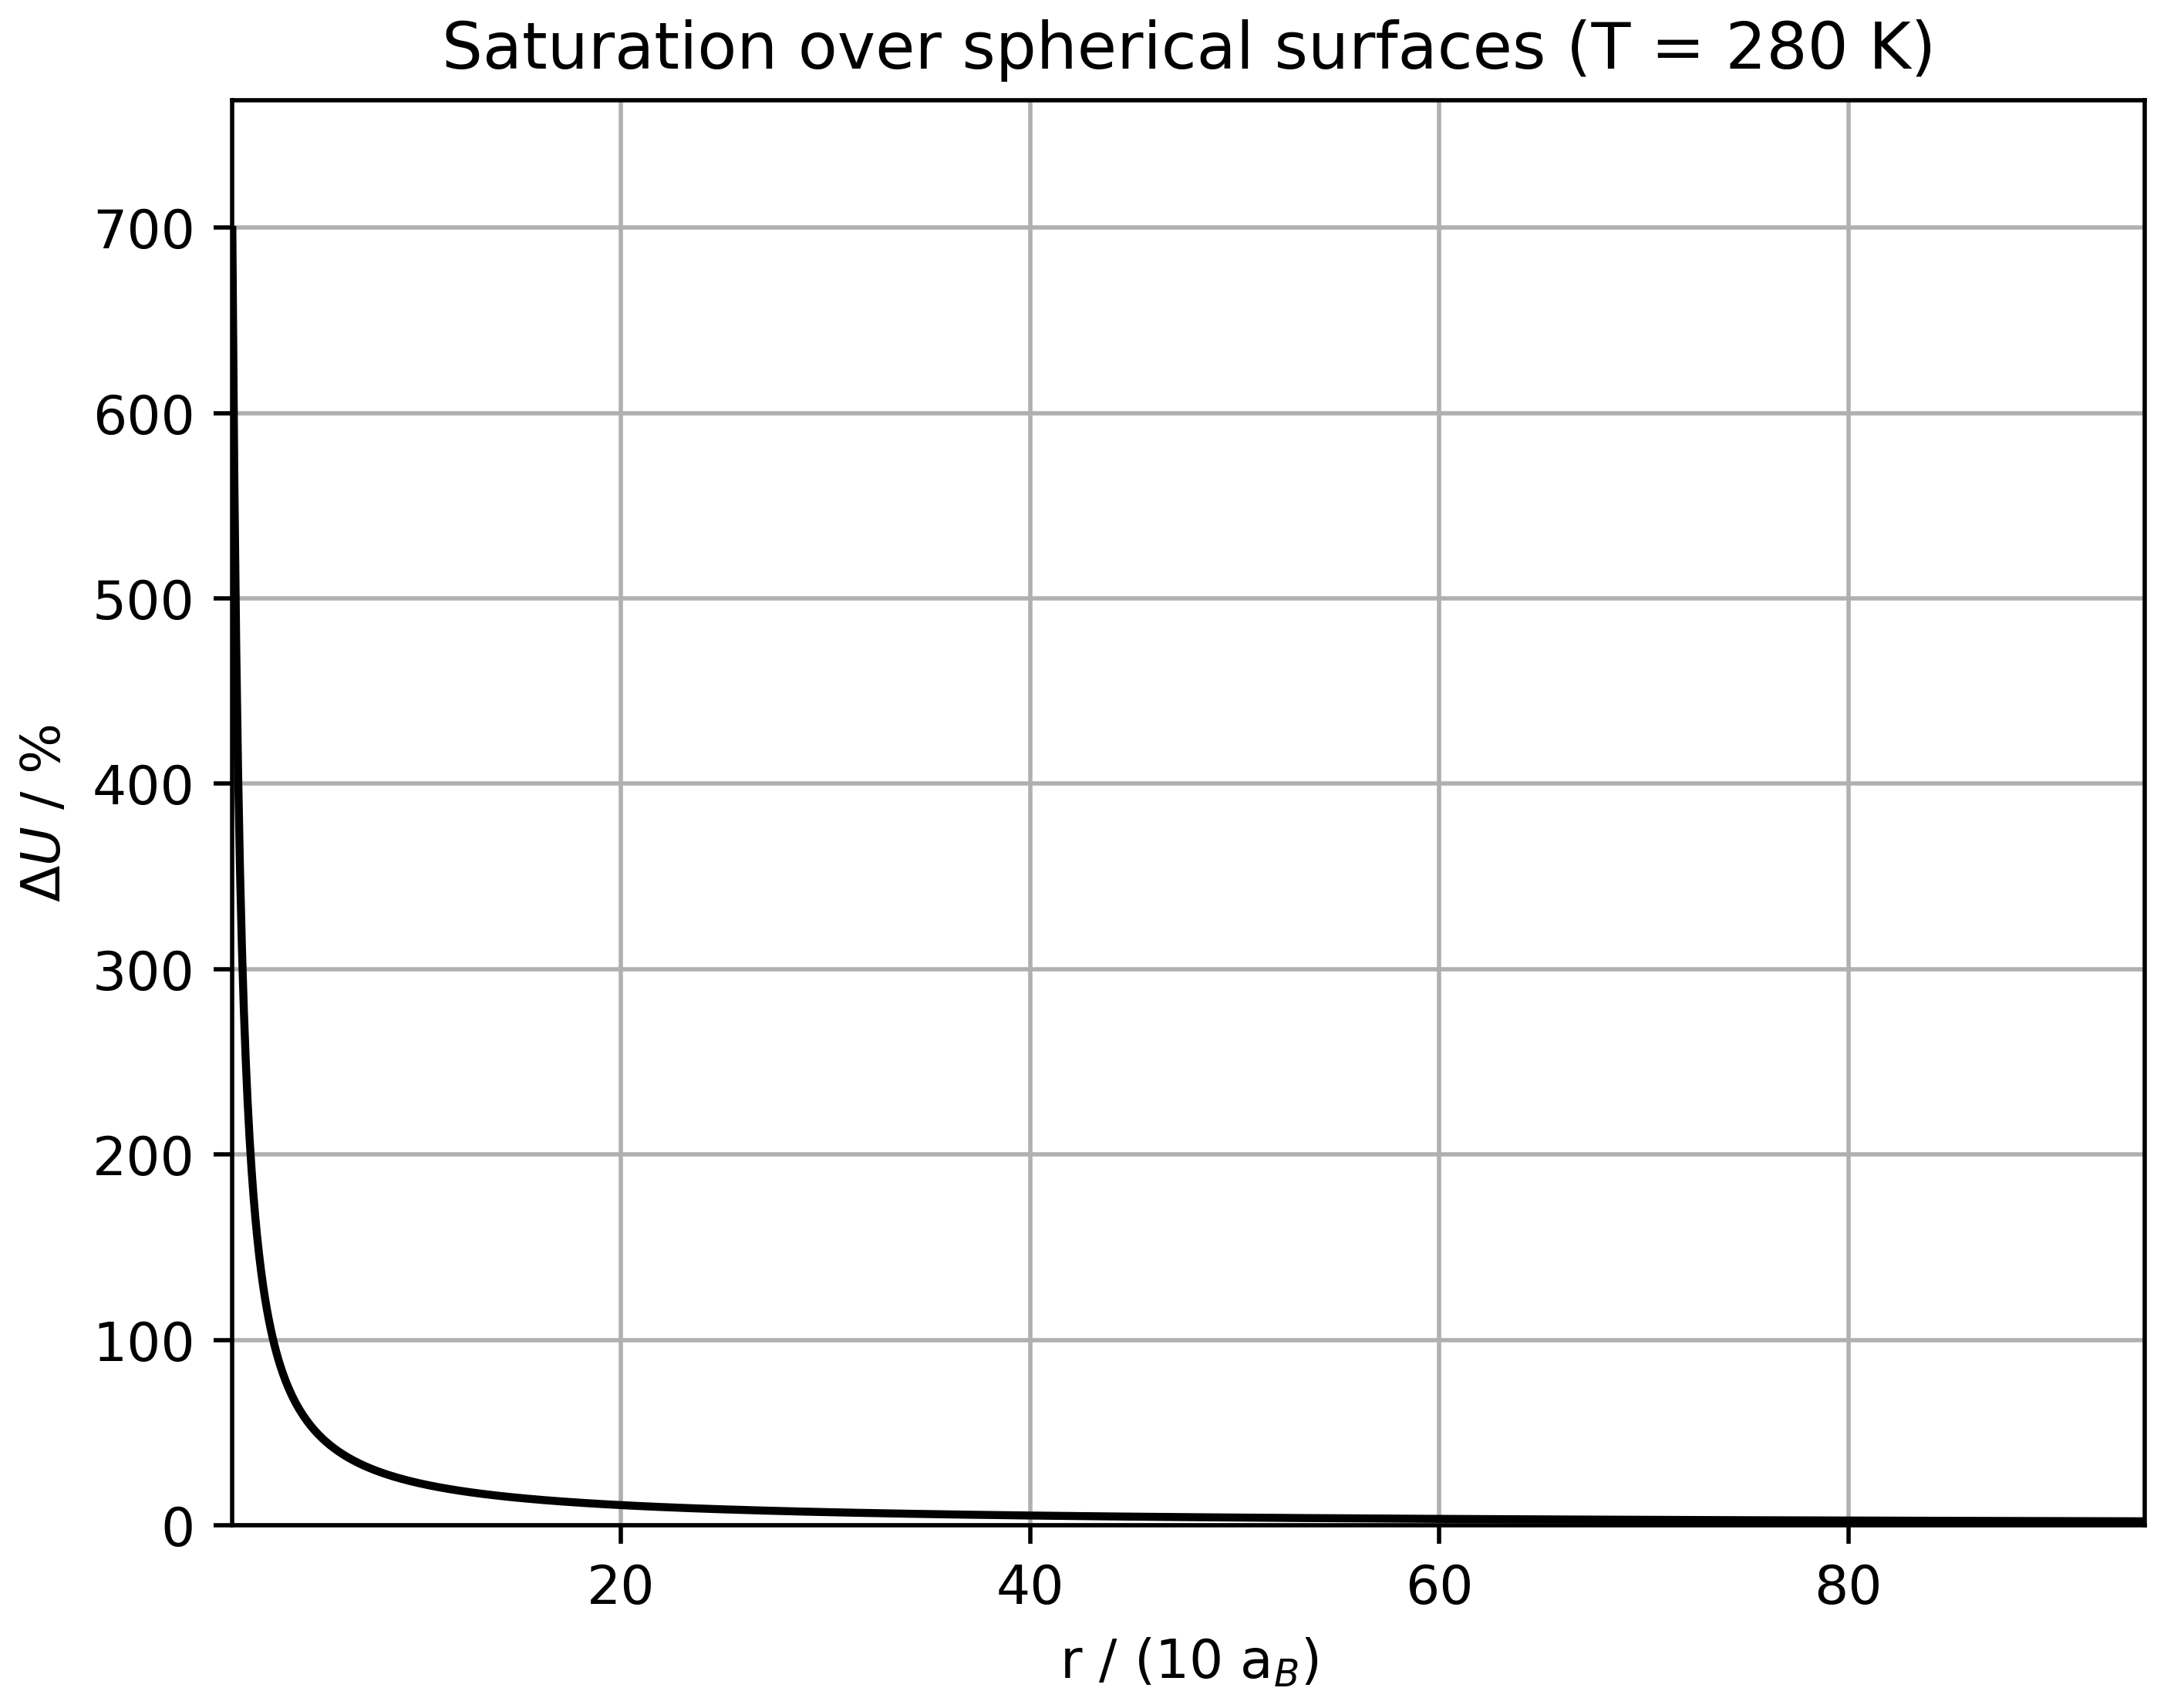
\includegraphics[width = 0.6\textwidth]{figs/kelvin_equation.png}
\caption{Differenz zwischen der Sättigungsfeuchte\index{Sättigungsfeuchte} über einer gekrümmten Oberfläche und über einer ebenen Oberfläche am Beispiel von Wasser.}
\label{fig:kelvin_equation}
\end{center}
\end{figure}

\section{Photonengas}
\label{sec:photonengas}\index{Photonengas}

Man stelle sich einen Hohlraum der Temperatur $T$ vor, der im Gleichgewicht mit elektromagnetischer Strahlung steht. Gesucht ist die spektrale Energiedichte $u\left(\omega\right)$ im Hohlraum. Die Eigenschaften elektromagnetischer Wellen wurden in Absch. \ref{sec:elektromagnetische_wellen} besprochen. Es handelt sich um Transversalwellen. Zeigt der Wellenvektor in z-Richtung, $\mathbf{k} = k\mathbf{e}_z$, folgt im Fall stehender Wellen für das elektrische Feld
%
\begin{align}
\mathbf{E}\left(z, t\right) = \left(E_{0, x}\mathbf{e}_x + E_{0, y}\mathbf{e}_y\right)\sin\left(kz\right)\sin\left(\omega t\right).
\end{align}
%
Eventuelle Phasen wurden vernachlässigt. Das B-Feld kann hieraus bestimmt werden. Der Hohlraum sei kubisch mit dem Volumen $V = L^3$, weiter seien die Wände metallisch. In diesem Fall verschwindet die Parallelkomponente des elektrischen Feldes an der Oberfläche, denn sonst würden Ströme angeregt und Energie würde dissipiert. Hieraus folgen die diskreten $k-$Werte
%
\begin{align}
k_iL = i\pi\Leftrightarrow k_i = \frac{\pi}{L}i
\end{align}
%
mit $i\in\mathbb{N}$ und $i\geq 1$, negative Werte von $i$ müssen vernachlässigt werden, weil dadurch keine neuen Lösungen entstehen. Summen über $k_i-$Werte können wieder durch Integrale ersetzt werden:
%
\begin{align}
\sum_{k_i}^{}\dotsc = \frac{L}{\pi}\int_0^\infty\dotsc dk = \frac{L}{2\pi}\int_{-\infty}^{\infty}\dotsc dk.
\end{align}
%
Für eine Summe über alle Moden im Hohlraum gilt
%
\begin{align}
\sum_{m = 1}^{2}\sum_{\mathbf{k}}^{}\dotsc = \frac{2V}{\left(2\pi\right)^3}\int\dotsc d^3k.
\end{align}
%
$m$ läuft dabei über die zwei möglichen Polarisationsrichtungen. Für die Energien $E = E\left(\mathbf{k}, m\right)$ gilt nach Glg. \eqref{eq:energy_photon}
%
\begin{align}
E\left(\mathbf{k}, m\right) = \hbar\omega\left(k\right) = \hbar ck.
\end{align}
%
Ein Mikrozustand $r$ des Systems ist durch die Angabe der Besetzungszahlen
%
\begin{align}
r = \left(n_{\mathbf{k}, m}\right)
\end{align}
%
gegeben, also die Anzahl der Anregungen für jede Schwingungsmode, eine Anregung ist ein Photon. Für die Energie $E_r\left(V\right)$ des Mikrozustandes ergibt sich
%
\begin{align}
E_r\left(V\right) = \sum_{m, \mathbf{k}}^{}\hbar\omega\left(k\right)n_{\mathbf{k}, m} = \hbar c\sum_{\mathbf{k}, m}^{}kn_{\mathbf{k}, m}.
\end{align}
%
Nun sind die mittleren Besetzungszahlen $\newoverline{n}_{\mathbf{k}, m}$ zu ermitteln. Hierfür geht man aus von der großkanonischen Zustandssumme eines Systems ohne Polarisationsfreiheitsgrad, also $m = 1$:
%
\begin{align}
Y & = \sum_r\exp\left[-\beta\left(E_r - \mu N_r\right)\right] = \sum_{n_{\mathbf{p}_1 = 0}}^{\infty}\exp\left[-\beta\left(E_{p_1} - \mu\right)n_{\mathbf{p}_1}\right]\cdot\sum_{n_{\mathbf{p}_2} = 0}^{\infty}\exp\left[-\beta\left(E_{p_2} - \mu\right)n_{\mathbf{p}_2}\right]\cdot\dotsc\nonumber\\
&\stackrel{\text{Glg. \eqref{eq:geometr_reihe}}}{=} \prod_{\mathbf{p}}^{}\frac{1}{1 - \exp\left(-\beta\left(E_p - \mu\right)\right)}.
\end{align}
%
Es folgt
%
\begin{align}
\newoverline{n}_{\mathbf{p}_i} & = \frac{1}{Y}\sum_rn_{\mathbf{p}_i}\exp\left[-\beta\left(E_r - \mu N_r\right)\right] = \frac{1}{Y}\sum_{n_{\mathbf{p}_1} = 0}^{\infty}\dotsc\sum_{n_{\mathbf{p}_i} = 0}^{\infty}\dotsc n_{\mathbf{p}_i}\exp\left[-\beta\left(E_{\mathbf{p}_i} - \mu\right)n_{\mathbf{p}_i}\right]\dotsc\nonumber\\
& = \frac{1}{Y}\sum_{n_{\mathbf{p}_1} = 0}^{\infty}\dotsc\left(\frac{1}{\beta}\frac{\partial}{\partial\mu}\sum_{n_{\mathbf{p}_i} = 0}^{\infty}\exp\left[-\beta\left(E_{\mathbf{p}_i} - \mu\right)n_{\mathbf{p}_i}\right]\right)\dotsc = \frac{1}{Y}\sum_{n_{\mathbf{p}_1} = 0}^{\infty}\dotsc\left(\frac{1}{\beta}\frac{\partial}{\partial\mu}\frac{1}{1 - \exp\left[-\beta\left(E_{\mathbf{p}_i} - \mu\right)\right]}\right)\dotsc\nonumber\\
& = \frac{1}{Y}\sum_{n_{\mathbf{p}_1} = 0}^{\infty}\dotsc\left(\frac{\exp\left[-\beta\left(E_{\mathbf{p}_i} - \mu\right)\right]}{\left(1 - \exp\left[-\beta\left(E_{\mathbf{p}_i} - \mu\right)\right]\right)^2}\right)\dotsc = \frac{\exp\left[-\beta\left(E_{\mathbf{p}_i} - \mu\right)\right]}{1 - \exp\left[-\beta\left(E_{\mathbf{p}_i} - \mu\right)\right]}.
\end{align}
%
Dies ist die \index{Bose-Verteilung}\textit{Bose-Verteilung}, sie gilt für Teilchen mit ganzzahligem Spin:
%
\begin{center}
\doublebox{\parbox{0.8\textwidth}{
\begin{center}
\begin{align}
\newoverline{n}_\mathbf{p} = \frac{1}{e^{\beta\left(E_\mathbf{p} - \mu\right)} - 1}
\end{align}
\end{center}
}}
\end{center}
%
Die Energieeigenwerte $E_r\left(V\right)$ hängen nicht von der Phononenanzahl $N$ ab, daher gilt
%
\begin{align}
\mu = \newoverline{\frac{\partial E_r\left(V\right)}{\partial N}} = 0, 
\end{align}
%
das chemische Potential verschwindet. Somit gilt
%
\begin{align}
\newoverline{n}_{\mathbf{k}, m} = \frac{1}{\exp\left(\beta E_k\right) - 1}.
\end{align}
%
Es folgt
%
\begin{align}
E\left(T, V\right) = \newoverline{E_r\left(T, V\right)} & = \sum_{m, \mathbf{k}}^{}E_k\newoverline{n_k} = \frac{2V}{\left(2\pi\right)^3}\int\frac{\hbar ck}{\exp\left(\beta\hbar ck\right) - 1}d^3k = \frac{2V}{\left(2\pi\right)^3}4\pi\int_{0}^{\infty}\frac{\hbar ck^3}{\exp\left(\beta\hbar ck\right) - 1}dk\nonumber\\
& = V\int_{0}^{\infty}\underbrace{\frac{\hbar}{c^3\pi^2}\frac{\omega^3}{\exp\left(\beta\hbar\omega\right) - 1}}_{ = u\left(\omega\right)}d\omega.
\end{align}
\begin{center}
\doublebox{\parbox{0.8\textwidth}{
\begin{center}
\begin{align}
u\left(\omega\right) = \frac{\hbar}{\pi^2c^3}\frac{\omega^3}{\exp\left(\frac{\hbar\omega}{k_BT}\right) - 1}.\label{eq:plancksche_strahlungsformel}
\end{align}
\end{center}
}}
\end{center}
%
Dies ist das \index{Planck'sches Strahlungsgesetz}\index{Strahlungsgesetz!Planck'sches}\textit{Planck'sche Strahlungsgesetz}. Die Vorstellungen dieses Abschnitts sind sehr speziell, jedoch gilt die Planck'sche Verteilung immer, wenn Materie der Temperatur $T$ mit elektromagnetischer Strahlung im Gleichgewicht steht. Von diesem Gleichgewicht ist aufgrund der hohen Geschwindigkeit der Wellen (Lichtgeschwindigkeit) immer auszugehen. Es kann jedoch Abweichungen im Spektrum geben, beispielsweise Absorptionslinien. Innerhalb eines Hohlraums im thermischen Gleichgewicht ist die Strahlung isotrop, daher gilt für die spektrale Strahldichte
%
\begin{align}
J\left(\omega\right) = \frac{u\left(\omega\right)}{4\pi}c = \frac{\hbar}{4\pi^3c^2}\frac{\omega^3}{\exp\left(\frac{\hbar\omega}{k_BT}\right) - 1}.
\end{align}
%
Die spektrale Intensität $I\left(\omega\right)$ einer strahlenden Oberfläche berechnet berechnet sich daraus zu
%
\begin{align}
I\left(\omega\right) & = \int_{\vartheta = 0}^{\pi/2}\int_{\phi = 0}^{2\pi}J\left(\omega\right)\cos\left(\vartheta\right)\sin\left(\vartheta\right)d\vartheta d\phi = 2\pi\frac{1}{2}J\left(\omega\right) = \frac{\hbar}{4\pi^2c^2}\frac{\omega^3}{\exp\left(\frac{\hbar\omega}{k_BT}\right) - 1}.
\end{align}
%
Integriert man dies über das gesamte Spektrum, folgt für die abgestrahlte Leistungsdichte
%
\begin{align}
\frac{P}{A} = \int_{0}^{\infty}I\left(\omega\right)d\omega = \frac{\hbar}{4\pi^2c^2}\int_{0}^{\infty}\frac{\omega^3}{\exp\left(\frac{\hbar\omega}{k_BT}\right) - 1}d\omega = \frac{k_B^4T^4}{4\pi^2c^2\hbar^3}\int_{0}^{\infty}\frac{x^3}{e^x - 1}d^x
\end{align}
%
Mit Glg. \eqref{eq:stefanboltzmann_help} folgt
%
\begin{align}
P = P\left(T\right) = \frac{k_B^4\pi^2}{60c^2\hbar^3}T^4.
\end{align}
%
Dies ist das \textit{Stefan-Boltzmann-Gesetz}, \index{Stefan-Boltzmann-Gesetz} man definiert
%
\begin{align}
\sigma \coloneqq\frac{k_B^4\pi^2}{60c^2\hbar^3}
\end{align}
%
als die \textit{Stefan-Boltzmann-Konstante}\index{Stefan-Boltzmann-Konstante}. Reale Körper emittieren bei einer Temperatur $T$ in die durch $\vartheta$ und $\varphi$ vorgegebene Richtung bei einer Kreisfrequenz $\omega$ eine von $J\left(\omega, T\right)$ um den Faktor
%
\begin{align}
\epsilon = \epsilon\left(\omega, T, \vartheta, \varphi\right)
\end{align}
%
abweichende spektrale Strahldichte:
%
\begin{align}
J_{\text{real}}\left(\omega, T, \vartheta, \varphi\right) = \epsilon\left(\omega, T, \vartheta, \varphi\right)J\left(\omega, T\right).
\end{align}
%
Den Faktor $\epsilon$ bezeichnet man als \textit{Emissivität}.\index{Emissivität} Man stelle sich eine kleine Fläche $dA$ auf der inneren Oberfläche des Hohlraums vor. Diese Fläche absorbiert eine Leistungsdichte
%
\begin{align}
\frac{dP_{\text{abs}}}{dA} = \int_{\omega = 0}^\infty\int_{\vartheta = 0}^{\pi/2}\int_{\varphi = 0}^{2\pi}\alpha\left(\omega, T, \vartheta, \varphi\right)J\left(\omega, T\right)\cos\left(\vartheta\right)\sin\left(\vartheta\right)d\varphi d\vartheta d\omega, 
\end{align}
%
hierbei wurde der Absorptionskoeffizient $\alpha\left(\omega, T, \vartheta, \varphi\right)$ eingeführt. Da von einem thermodynamischen Gleichgewicht ausgegangen wird, gilt für die emittierte Leistungsdichte
%
\begin{align}
\frac{dP_{\text{emt}}}{dA} = \int_{\omega = 0}^\infty\int_{\vartheta = 0}^{\pi/2}\int_{\varphi = 0}^{2\pi}\epsilon\left(\omega, T, \vartheta, \varphi\right)J\left(\omega, T\right)\cos\left(\vartheta\right)\sin\left(\vartheta\right)d\varphi d\vartheta d\omega = \frac{dP_{\text{abs}}}{dA}.
\end{align}
%
Daraus folgt
%
\begin{align}
\int_{\omega = 0}^\infty\int_{\vartheta = 0}^{\pi/2}\int_{\varphi = 0}^{2\pi}\left(\epsilon\left(\omega, T, \vartheta, \varphi\right) - \alpha\left(\omega, T, \vartheta, \varphi\right)\right)J\left(\omega, T\right)\cos\left(\vartheta\right)\sin\left(\vartheta\right)d\varphi d\vartheta d\omega = 0.
\end{align}
%
Da die spektrale Energiedichte des Hohlraums konstant ist, gilt sogar
%
\begin{align}
\int_{\vartheta = 0}^{\pi/2}\int_{\varphi = 0}^{2\pi}\left[\epsilon\left(\omega, T, \vartheta, \varphi\right) - \alpha\left(\omega, T, \vartheta, \varphi\right)\right]\sin\left(\vartheta\right)\cos\left(\vartheta\right)d\varphi d\vartheta = 0.
\end{align}
%
Definiert man
%
\begin{align}
\epsilon\left(\omega, T\right) \coloneqq\int_{\vartheta = 0}^{\pi/2}\int_{\varphi = 0}^{2\pi}\epsilon\left(\omega, T, \vartheta, \varphi\right)\sin\left(\vartheta\right)\cos\left(\vartheta\right)d\varphi d\vartheta.
\end{align}
%
und analog für den Absorptionskoeffizienten, folgt
%
\begin{align}
\epsilon\left(\omega, T\right) = \alpha\left(\omega, T\right).
\end{align}
%
Nun betrachtet man spezifisch die durch $\vartheta$ und $\varphi$ vorgegebene Richtung. Hier geht von $dA$ die spektral Strahldichte
%
\begin{align}
& J_\text{out}\left(\omega, T\right) = J\left(\omega, T\right)\nonumber\\
& = J\left(\omega, T\right)\left(\epsilon\left(\omega, T, \vartheta, \varphi\right) + \int_{\varphi' = 0}^{2\pi}\int_{\vartheta' = 0}^{\pi/2}s\left(\vartheta', \varphi', \vartheta, \varphi, \omega, T\right)\cos\left(\vartheta'\right)\sin\left(\vartheta'\right)d\vartheta'd\varphi'\right)
\end{align}
%
aus. Der Klammerausdruck ergibt sich zu Eins. Dabei wurde der \textit{Streuquerschnitt}\index{Streuquerschnitt} $s\left(\vartheta', \varphi', \vartheta, \varphi, \omega, T\right)$ definiert. Er beschreibt, in welchem Maße Strahlung, die aus der Richtung $\left(\vartheta', \varphi'\right)$ einfällt, in die Richtung $\left(\vartheta, \varphi\right)$ umgelenkt wird, ohne zwischendurch absorbiert und wieder emittiert zu werden. Für die einfallende spektrale Strahldichte gilt
%
\begin{align}
& J_\text{in}\left(\omega, T\right) = J\left(\omega, T\right)\nonumber\\
& = J\left(\omega, T\right)\left(\alpha\left(\omega, T, \vartheta, \varphi\right) + \int_{\varphi' = 0}^{2\pi}\int_{\vartheta' = 0}^{\pi/2}s\left(\vartheta, \varphi, \vartheta', \varphi', \omega, T\right)\cos\left(\vartheta'\right)\sin\left(\vartheta'\right)d\vartheta'd\varphi'\right)
\end{align}
%
Der Klammerausdruck muss sich wieder zu Eins ergeben. Da die Maxwell-Gleichungen genau wie die Schrödinger-Gleichung invariant gegen Zeitumkehr sind, gilt
%
\begin{align}
s\left(\vartheta, \varphi, \vartheta', \varphi', \omega, T\right) = s\left(\vartheta', \varphi', \vartheta, \varphi, \omega, T\right).
\end{align}
%
Daraus folgt
%
\begin{align}
\epsilon\left(\omega, T, \vartheta, \varphi\right) = \alpha\left(\omega, T, \vartheta, \varphi\right)
\end{align}
%
Dies bezeichnet man als \textit{Kirchhoff'sches Strahlungsgesetz}\index{Kirchhoff'sches Strahlungsgesetz}\index{Strahlungsgesetz!Kirchhoff'sches}. Da ein Körper nie mehr als die auf ihn treffende Strahlung absorbieren kann, gilt $\alpha\leq1$, somit folgt
%
\begin{align}
\epsilon\leq1.
\end{align}
%
Körper mit $\epsilon\left(\vartheta, \varphi, \omega\right) = 1$ bezeichnet man als \textit{schwarze Körper}, \index{schwarzer Körper}\index{Körper!schwarzer} das Stefan-Boltzmann-Gesetz gilt also nur für schwarze Körper.

\part{Herrschende Gleichungen}
\label{part:herrschende_gleichungen}\index{herrschende Gleichung}\index{Gleichungen!herrschende}

\chapter{\normalfont\textsc{Zustand der Atmosphäre}}
\label{chap:zustand_der_atmosphaere}\index{Zustand!der Atmosphäre}\index{Atmosphäre!Zustand}

Die herrschenden Gleichungen bilden das die zeitliche Entwicklung der Atmosphäre festlegende Gleichungssystem. Zunächst muss jedoch ihr Zustand beschrieben werden können.

Ein Teilchen ist ein kleines Luftvolumen $\Delta V$, was so groß ist, dass im langzeitlichen Mittel eine so große Anzahl Gasmoleküle darin enthalten ist, dass von einem kontinuierlichen Materiebild ausgegangen werden kann. Die Atmosphäre $A\subseteq\mathbb{R}^3$ offen ist die Gashülle der Erde. Die Offenheit ist sinnvoll, damit in jedem Punkt eine Richtungsableitung in jede Richtung möglich ist. Die Definition der Obergrenze hängt vom zu behandelnden Problem ab. An der Untergrenze wird die Atmosphäre durch die Erdoberfläche begrenzt, inklusive der dort stattfindenden Bewegungen, somit ist die Menge $A$ zeitabhängig, $A = A\left(t\right)$. Alle meteorologischen Felder werden als so oft differenzierbar vorausgesetzt, wie es für die Rechnungen benötigt wird. \textit{Luft}\index{Luft} besteht aus \textit{trockener Luft}\index{Luft!trockene}\index{trockene Luft} und \textit{Tracern}\index{Tracer}. Zu diesen zählen:
%
\begin{itemize}
\item Wasserdampf
\item flüssiges oder festes Wasser
\item Aerosole, die nicht aus Wasser bestehen
\item in variabler Konzentration vorhandene gasförmige Komponenten
\end{itemize}
%
\section{Gasphase}
\label{sec:gasphase}\index{Gasphase}

\textit{Feuchte Luft}\index{Luft!feuchte}\index{feuchte Luft} ist eine Mischung aus trockener Luft und Wasserdampf. Die Anzahl der berücksichtigen \textit{Tracerklassen}\index{Tracerklasse}, insbesondere der \textit{Kondensatklassen}\index{Kondensatklasse}, wird dann als genügend angesehen, wenn falsche Vorhersagen nicht mehr auf Grobheiten im für die Vorhersage verwendeten Gleichungssystem, sondern auf Fehler in den Anfangs- und/oder Randbedingungen zurückzuführen sind. Folgende Zustandsgrößen werden definiert:
%
\begin{itemize}
\item Die Dichte trockener Luft\index{Dichte!trockener Luft} $\rho_d:A\to\mathbb{R}$ wird definiert durch

\begin{align}
\rho_d \coloneqq \frac{1}{\Delta V}\sum_{i = 1}^{N_d}m_i^{(d)}.
\end{align}

Hierbei ist $N_d$ die Anzahl der Gasatome außer H$_2$O und anderen gesondert betrachteten Spurengasen, die im Volumen $\Delta V$ vorhanden sind, und die $m_i^{(d)}$ sind ihre Massen.
\item Der \index{Windvektor}\textit{Windvektor} $\mathbf{v}:A\to\mathbb{R}^3$ wird definiert durch

\begin{align}
\mathbf{v} \coloneqq \frac{1}{\sum_{j = 1}^{N_g}m_j^{(g)}}\sum_{i = 1}^{N_g}m_i^{(g)}\mathbf{v}_i^{(g)},\label{eq:def_windvector}
\end{align}

wobei $\mathbf{v}_i^{(g)}$ die Geschwindigkeit des $i-$ten Moleküls des gasförmigen Anteils der Luft in $\Delta V$ ist.
\item Die Temperatur\index{Temperatur} $T:A\to\mathbb{R}$ der feuchten Luft.
\item $p:A\to\mathbb{R}$\index{Druck} sei der Druck.

\end{itemize}

\section{Zweiter Kontinuumsübergang}
\label{sec:zweiter_kontinuumsuebergang}\index{Zweiter Kontinuumsübergang}\index{Kontinuumsübergang!Zweiter}

Die Herleitung der Navier-Stokes-Gleichungen\index{Navier-Stokes-Gleichung} beruht auf einer kontinuierlichen Vorstellung von Materie, welche durch einen Kontinuumsübergang\index{Kontinuumsübergang} motiviert wurde. Der Kontinuumsübergang ist eine heuristische Idee, die auf der Annahme beruht, dass Materie irgendwann kontinuierlich wird, wenn man nur so weit herauszoomt, dass die Grobkörnigkeit der Materie in Form von Atomen und Molekülen verschwimmt. Mathematisch bedeutet dies, anstatt eine Anzahl von Bahnkurven stetig differenzierbare Felder zur Beschreibung des Systems zu verwenden.

Mit einem ähnlichen Problem ist man konfrontiert, wenn man Phasenübergänge und Kondensate in die Beschreibung mit aufnimmt. Man könnte nun die Kondensate durch Bahnkurven beschreiben, während man die Gasphase weiterhin als Fluid auffasst. Dies hat jedoch die zwei Nachteile: Zunächst muss man für so eine Formulierung die technische Frage beantworten, ab welcher Größe etwas also Kondensat aufgefasst wird; außerdem ist der Rechenaufwand hierfür enorm. Stattdessen macht man den sogenannten \textit{Zweiten Phasenübergang}\index{Zweiter Phasenübergang}\index{Phasenübergang!Zweiter}, welcher auch die Massendichten und sonstigen Eigenschaften der Kondensate als stetig differenzierbare Funktionen auffasst. Dies ist natürlich nicht exakt in einem Sinne in dem die Maxwell-Gleichungen exakt sind, das prinzipielle Problem ist jedoch schon in den Navier-Stokes-Gleichungen\index{Navier-Stokes-Gleichung} selbst angelegt.

Folgende Zustandsgrößen werden für die Kondensate, die von nun an auch als \textit{Tracer}\index{Tracer} bezeichnet werden, zusätzlich eingeführt:

\begin{itemize}
\item Die Dichten der Tracerklassen $\rho_i:A\to\mathbb{R}$ werden analog zu $\rho_d$ definiert.
\item Die $Q_i:A \to \mathbb{R}$ seien die Ladungsdichten der Tracer\index{Ladungsdichte!der Tracer}.
\item Die Massenstromdichte\index{Massenstromdichte} $\mathbf{j}_i:A\to\mathbb{R}^3$ der $i-$ten Tracerklasse wird definiert durch

\begin{align}
\mathbf{j}_i \coloneqq\rho_i\sum_{k = 1}^{N_i}\mathbf{v}_k^{(i)}, 
\end{align}

wobei $\mathbf{v}_k^{(i)}$ die Geschwindigkeit des $k-$ten Teilchens der entsprechenden Tracerklasse in $\Delta V$ ist.
\item Die Temperatur $T_i:A\to\mathbb{R}$ sei diejenige der $i-$ten Tracerklasse, alle Teilchen einer Klasse sollen die gleiche Temperatur haben. DIe gasförmigen Tracer haben die Temperatur der feucten Luft.
\item Weiterhin betrachtet man das Feld der spektralen Strahldichte\index{spektrale Strahldichte}\index{Strahldichte!spektrale} $L_\lambda:A\times\left[0, \infty\right)\times\left[0, \pi\right]\times\left[0, 2\pi\right)\to\mathbb{R}$.
\item Das \textit{elektrische Feld}\index{elektrisches Feld}\index{Feld!elektrisches} $\mathbf{E}$ sowie die \textit{magnetische Flussdichte}\index{magnetische Flussdichte}\index{Flussdichte!magnetische} $\mathbf{B}$ müssen benefalls berücksichtigt werden (z. B. für Gewitter und die \textit{Ionosphäre}\index{Ionosphäre}).
\end{itemize}
%
Die Gesamtheit all dieser Größen ist ein \textit{atmosphärischer Zustand}\index{Zustand!atmosphärischer}\index{atmosphärischer Zustand} $Z$. Ziel dieses Kapitels ist die Formulierung prognostischer Gleichungen so, dass durch Anfangsbedingungen und Randbedingungen die Zustandstrajektorie festgelegt ist. Dabei wird jeder Zustand als quasistationärer Zustand\index{quasistationärer Zustand}\index{Zustand!quasistationärer} betrachtet. Durch thermodynamische Zustandsgleichungen oder weitere diagnostische Gleichungen, die aus genäherten oder ungenäherten Relationen zwischen den Elementen von $Z$ hervorgehen, kann ein Zustand bereits durch eine echte Teilmenge von $Z$ oder durch eine Bijektion auf dieser Teilmenge festgelegt sein.

Die $i-$te Kondensatklasse habe die \textit{mikroskopische Dichte}\index{Dichte!mikroskopische}\index{mikroskopische Dichte} $\rho_i'$, damit ist beispielsweise die Dichte des Wassers $\sim$ $10^3$ kgm$^{-3}$ gemeint in Abgrenzung zur über ein Teilchen gemittelten Dichte. Die $\rho_i'$ werden als Konstanten angenommen, die nicht von äußeren Bedingungen abhängen, für sie gilt 
%
\begin{align}
\rho_i' = \frac{m_i}{V_i}, 
\end{align}
%
wobei $m_i$ die Masse der Komponente $i$ ist und $V_i$ das von ihr eingenommene Volumen. Die Dichte der Luft ergibt sich allgemein zu
%
\begin{align}
\rho = \frac{m_g + \sum_{i \in \left\lbrace\text{Kondensatklassen}\right\rbrace}m_i}{V_g + \sum_{i \in \left\lbrace\text{Kondensatklassen}\right\rbrace} V_i}.
\end{align}
%
Für die Dichte des Anteils $\rho_i$ gilt allgemein
%
\begin{align}
\rho_i = \frac{m_i}{v}_h = \frac{m_i}{V_g + \sum_{i \in \left\lbrace\text{Kondensatklassen}\right\rbrace}V_i}.
\end{align}
%
Für die Dichte $\rho_g$ der gasförmigen Luft gilt
%
\begin{align}
\rho_g = \frac{m_g}{v}_h = \frac{m_g}{V_g + \sum_{i \in \left\lbrace\text{Kondensatklassen}\right\rbrace}V_i}.
\end{align}
%
Für die mikroskopischen Dichten der gasförmigen Luft erhält man
%
\begin{align}
\rho_g' & = \frac{m_g}{V_g} = \frac{m_g}{V - \sum_{i \in \left\lbrace\text{Kondensatklassen}\right\rbrace}V_i} = \frac{1}{\frac{V}{m_g} - \sum_{i \in \left\lbrace\text{Kondensatklassen}\right\rbrace}\frac{V_i}{m_g}}\nonumber\\
& = \frac{1}{\frac{1}{\rho_g} - \sum_{i \in \left\lbrace\text{Kondensatklassen}\right\rbrace}\frac{V_i}{m_i}\frac{m_i}{m_g}} = \frac{\rho_g}{1 - \sum_{i \in \left\lbrace\text{Kondensatklassen}\right\rbrace}^{}\frac{\rho_i}{\rho_i'}}.
\end{align}
%
Die mikroskopische Dichte des Wasserdampfes $\rho_v'$ bezeichnet man auch als \textit{mikroskopische Feuchte}\index{Feuchte!mikroskopische}\index{mikroskopische Feuchte}. Für sie gilt analog
%
\begin{align}
\rho_v' = \frac{m_v}{V_g} = \frac{\rho_v}{1 - \sum_{i \in \left\lbrace\text{Kondensatklassen}\right\rbrace}^{}\frac{\rho_i}{\rho_i'}}.
\end{align}
%
Für die Zustandsgleichung von Luft gilt somit
%
\begin{center}
\doublebox{\parbox{0.8\textwidth}{
\begin{center}
\begin{align}
p = T_gR_g\rho_g'.
\end{align}
\end{center}
}}
\end{center}

\subsection{Deskriptiver Informationsverlust}
\label{sec:deskriptiver_informationsverlust}\index{Wolkenmikrophysik!Informationsverlust!deskriptiver}\index{Informationsverlust!deskriptiver!Wolkenmikrophysik}

In der statistischen Physik geht man bei der Beschreibung vom Mikrozustand zum Makrozustand über und sieht diese Beschreibung als statistisch vollständig an. In ähnlicher Weise kann man sich fragen, ob die in den vorangegangenen beiden Abschnitten entwickelte Beschreibung vollständig ist. Sie wäre dies (unter Annahme des Zweiten Kontinuumsübergangs) nur dann, wenn man unendlich viele Tracerklassen einführt und in jeder Teilchenklase wiederum eine kontinuierliche Temperaturverteilung annimmt. Bis auf die einschränkende Annahme, dass alle Teilchen einer Tracerklasse\index{Tracerklasse} die gleiche Temperatur haben, hat die obige Beschreibung also das Potential eine unter gewissen Annahmen vollständige Beschreibung zu sein.

\subsection{Forcings und Zeitableitungen}
\label{sec:forcings_und_zeitableitungen}\index{Forcing}

Phasenübergangsraten spielen für den Ersten Hauptsatz der Thermodynamik eine Rolle, da sie mit latenten Wärmeflüssen verbunden sind, genauso wie für die Kontinuitätsgleichungen, die sie Massenflüsse sind. Der Erste Hauptsatz wird jedoch materiell für ein bestimmtes Teilchen formuliert und nicht lokalzeitlich wie die Kontinuitätsgleichung. Es stellt sich die Frage, ob bei den Phasenübergangsraten eine Unterscheidung zwischen totaler und lokalzeitlicher Ableitung auftritt, da es sich bei diesen Größen ja auch um Zeitableitungen handelt. Um diese Frage zu beantworten, stelle man sich ein Messgerät vor, welches die Masse $m\left(t\right)$ misst, die bis zu einem Zeitpunkt $t>0$ in einem ortsfesten Kontrollvolumen $V$ die Phase gewechselt habe. Für die Phasenübergangsrate $q$ misst man
%
\begin{align}
q = \frac{m\left(t\right)}{tV}.
\end{align}
%
Man stelle sich ein zweites Messgerät vor, was die Masse $m'\left(t\right)$ misst, die bis zu einem Zeitpunkt $t>0$ in einem mit dem Windfeld mitbewegten Teilchen $V'\left(t\right)$ die Phase gewechselt hat. Es sei $V'\left(0\right) = V\left(0\right)$. Dann misst dieses Messgerät für die Phasenübergangsrate
%
\begin{align}
q' = \frac{m'\left(t\right)}{tV'\left(t\right)}.
\end{align}
%
Im Fall $t\to 0$ geht $V'\to V$. Daher gilt
%
\begin{align}
\lim\limits_{t \to 0}\left(q - q'\right) & = \lim\limits_{t \to 0}\left[\frac{m\left(t\right)}{Vt} - \frac{m'\left(t\right)}{V'\left(t\right)t}\right] = \lim_{t \to 0}\frac{m\left(t\right)}{Vt} - \lim\limits_{t\to 0}\frac{m'\left(t\right)}{V'\left(t\right)t}\nonumber\\
& = \frac{1}{V}\lim\limits_{t \to 0}\frac{m\left(t\right)}{t} - \lim\limits_{t\to0}\frac{1}{V'\left(t\right)}\lim\limits_{t \to 0}\frac{m'\left(t\right)}{t}\nonumber\\
& = \frac{1}{V}\lim\limits_{t \to 0}\frac{m\left(t\right)}{t} - \frac{1}{v}_h\lim\limits_{t \to 0}\frac{m'\left(t\right)}{t} = \frac{1}{v}_h\lim\limits_{t \to 0}\frac{m\left(t\right) - m'\left(t\right)}{t}
\end{align}
%
nach den Rechenregeln für Funktionsgrenzwerte. Mit der wahren orts- und zeitabhängigen Kondensationsrate $q_r\left(\mathbf{r}, t\right)$ kann man
%
\begin{align}
m\left(t\right) = \int_{0}^t\int_{V}q_{r}\left(\mathbf{r}, t\right)d^3rdt'
\end{align}
%
sowie
%
\begin{align}
m'\left(t\right) = \int_{0}^t\int_{V'\left(t\right)}q_{r}\left(\mathbf{r}, t\right)d^3rdt'
\end{align}
%
notieren. Damit erhält man
%
\begin{align}
m\left(t\right) - m'\left(t\right) & = \int_{0}^t\int_{V}q_{r}\left(\mathbf{r}, t\right)d^3rdt' - \int_{0}^t\int_{V'\left(t\right)}q_{r}\left(\mathbf{r}, t\right)d^3rdt'\nonumber\\
& = \int_{0}^t\left[\int_{V}q_{r}\left(\mathbf{r}, t\right)d^3r - \int_{V'\left(t\right)}q_{r}\left(\mathbf{r}, t\right)d^3r\right]dt'.
\end{align}
%
Nach dem Hauptsatz der Differenzial- und Integralrechnung folgt
%
\begin{align}
\lim\limits_{t \to 0}\frac{m\left(t\right) - m'\left(t\right)}{t} & = \frac{1}{V}\lim\limits_{t \to 0}\left[\int_{V}q_{r}\left(\mathbf{r}, t\right)d^3r - \int_{V'\left(t\right)}q_{r}\left(\mathbf{r}, t\right)d^3r\right] = 0.
\end{align}
%
Also ist $q - q' = 0$ für den Grenzfall $t\to 0$. Für die Phasenübergangsraten misst man also im System des Teilchens das Gleiche wie im ruhenden System, sodass hier die Unterscheidung zwischen totaler und lokalzeitlicher Zeitableitung nicht auftritt. Dies gilt analog für alle anderen Quellstärken und Forcings.

\chapter{\normalfont\textsc{Kontinuitätsgleichungen}}
\label{chap:kontinuitätsgleichungen}\index{Kontinuitätsgleichung}

Die Kontinuitätsgleichung ist die Bilanzgleichung der Masse. Sei $\Omega\subseteq\mathbb{R}^3$ eine offene Teilmenge, $\rho$ eine Dichte und $\mathbf{j}$ die entsprechende Flussdichte. Dann gilt mit dem Gaußchen Satz und einer Quelldichte $Q$
%
\begin{align}
\frac{\partial}{\partial t}\int_\Omega\rho d^3r &= -\int_{\partial \Omega}\mathbf{j}\cdot d\mathbf{n} + \int_\Omega Qd^3r = -\int_\Omega\nabla\cdot\mathbf{j} - Q d^3r\nonumber\\
\Rightarrow \int_\Omega\frac{\partial\rho}{\partial t} + \nabla\cdot\mathbf{j} - Qd^3r &= 0.\label{eq:deriv_cont_1}
\end{align}
%
Da der Integrand stetig ist, ist selbiger bereits homogen und konstant gleich Null. Gilt nämlich $\left|\frac{\partial\rho}{\partial t} + \nabla\cdot\mathbf{j} - Q\right|>\epsilon>0$ an einer Stelle $\mathbf{r}_0\in\Omega$, so exisitiert eine offene Umgebung $\omega\subseteq\Omega$ mit $\mathbf{r}_0\in\omega$ und $\int_\omega\frac{\partial\rho}{\partial t} + \nabla\cdot\mathbf{j} - Qd^3r \not= 0$ im Widerspruch zu Glg. \eqref{eq:deriv_cont_1}. Es gilt somit
%
\begin{align}
\frac{\partial\rho}{\partial t} + \nabla\cdot\mathbf{j} = Q.\label{eq:cont_general}
\end{align}
%
In Termen des spezifischen Volumens $\alpha$ kannman dies als
%
\begin{align}
-\frac{1}{\alpha^2}\frac{\partial\alpha}{\partial t} - \frac{1}{\alpha^2}\mathbf{v}\cdot\nabla\alpha + \frac{1}{\alpha}\nabla\cdot\mathbf{v} = 0 && \Leftrightarrow \frac{\partial\alpha}{\partial t} = \alpha\nabla\cdot\mathbf{v} - \mathbf{v}\cdot\nabla\alpha.\label{eq:cont_spec_volume}
\end{align}
%
notieren. Dies notiert man nun separat für alle Komponenten der Luft:
%
\begin{center}
\doublebox{\parbox{0.8\textwidth}{
\begin{center}
\begin{align}
\frac{\partial\rho_d}{\partial t} + \nabla\cdot\mathbf{j}_d & = Q_d\label{eq:kont_d_pre}\\
\frac{\partial\rho_v}{\partial t} + \nabla\cdot\mathbf{j}_v & = Q_v\label{eq:kont_v_pre}\\
\frac{\partial\rho_i}{\partial t} + \nabla\cdot\mathbf{j}_i & = Q_i\label{eq:kont_i_pre}
\end{align}
\end{center}
}}
\end{center}
%
Dabei gelten
%
\begin{align}
\mathbf{j}_d = \rho_d\mathbf{v} - D_d\nabla\rho_d, && \mathbf{j}_v = \rho_v\mathbf{v} - D_v\nabla\rho_v.
\end{align}
%
Die $D_d, D_v$ sind die Diffusionskoeffizienten für trockene bzw. feuchte Luft. Man kann zunächst
%
\begin{align}
Q_d = 0
\end{align}
%
festhalten. Nun sollen die $Q_x$ in den Glg.en \eqref{eq:kont_d_pre} - \eqref{eq:kont_i_pre} genauer angegeben werden. Es gibt fünf Prozesse, die zu ihnen beitragen:
%
\begin{itemize}
\item Diffusion
\item Phasenübergänge
\item Kollisionen
\item Zerfälle
\item bei Gasen, Ionen und Elektronen auch chemische Reaktionen und Strahlungswechselwirkung
\end{itemize}
%
Der letzte Punkt wird im Rest des Abschnitts ausgeklammert, hier soll es nur um die Kondensate gehen. Diffusion gibt es nur bei den gasförmigen Bestandteilen, also tritt in $Q_d$ ein Term $D_d\Delta\rho_d$ und in $Q_v$ ein Term $D_v\Delta\rho_v$ auf, hierbei sind $D_d$ und $D_v$ die Diffusionskoeffizienten von trockener Luft bzw. Wasserdampf in Luft. Trockene Luft ist von den übrigen Prozessen nicht betroffen, sodass
%
\begin{align}
Q_d = D_d\Delta\rho_d
\end{align}
%
gilt.

Treffen sich zwei Partikel der Kondensatklassen $j$ und $k$, so kann man eine Wahrscheinlichkeit $0\leq P_{j, k}\leq 1$ dafür angeben, dass sie danach einen Partikel bilden. Dieser hat eine wohldefinierte Klasse $R_{j, k}$. Weiterhin sei $\sigma_{j, k}$ der Wirkungsquerschnitt der Kollisionen von Partikeln der Klassen $j$ und $k$. Sind $j$ beispielsweise Kugeln mit Radius $r_j$ und $k$ Kugeln mit Radius $r_k$, so gilt $\sigma_{j, k} = \pi\left(r_j + r_k\right)^2$. Die gemittelte Relativgeschwindigkeit zwischen den Teilchen der Klassen $j$ und $k$ sei $\newoverline{v_{\text{rel}}}\left(j, k\right)$. Dann durchfliegt ein Partikel der Klasse $j$ in der Zeit $t$ relativ zu den Partikeln der Klasse $k$ ein Volumen $\sigma_{j, k}\newoverline{v_{\text{rel}}}\left(j, k\right)t$. Die mittlere Stoßzeit $\tau_{j, k}$ ist dadurch definiert, dass man fordert, dass sich in diesem Volumen genau ein Teilchen der Klasse $k$ aufhält, also
%
\begin{align}
n_k\sigma_{j, k}\newoverline{v_{\text{rel}}}\left(j, k\right)\tau_{j, k} &\hastobe 1.
\end{align}
%
Alle Teilchen der Gruppe $j$ nehmen an Stoßprozessen teil, deshalb ist die Gesamt-Stoßrate von Teilchen $j$ mit Partikeln $k$ gegeben durch
%
\begin{align}
\frac{n_j}{\tau_{j, k}} &= n_jn_k\sigma_{j, k}\newoverline{v_{\text{rel}}}\left(j, k\right).
\end{align}
%
Ist $\newtilde{m}_i$ die Masse der Teilchen der Gruppe $i = R_{j, k}$, so ergibt sich eine entsprechende Quellstärke
%
\begin{align}
\newtilde{m}_i\sigma_{j, k}n_jn_k\newoverline{v_{\text{rel}}}\left(j, k\right)P_{j, k}.
\end{align}
%
Weiterhin muss auch ein negativer Anteil der Quellstärke berücksichtigt werden, der dadurch zustande kommt, dass Teilchen ihrer ursprünglichen Kondensatklasse verlorengehen, wenn sie sich mit anderen Teilchen verbinden. Dies führt zu
%
\begin{align}
Q_i^{(\text{Kollisionen})} = \newtilde{m}_i\sum_{j}\sum_{k\leq j}^{}\sigma_{j, k}n_jn_k\newoverline{v_{\text{rel}}}\left(j, k\right)P_{j, k}\left(\delta_{i, R_{j, k}} - \delta_{j, i} - \delta_{k, i}\right).
\end{align}
%
Dies erfordert wegen Massenerhaltung, dass die Teilchenmassen $\newtilde{m}_i$ ganzzahlige Vielfache einer minimalen Masse sind, damit bei Kollisionen keine Masse artifiziell verschwindet oder entsteht.

Nun werden Zerfallsprozesse untersucht. Für die Änderung einer Teilchendichte $n_j$ durch Zerfälle gilt
%
\begin{align}
dn_j = -n_j\lambda_jdt\Leftrightarrow\frac{dn_j}{dt} = -\lambda_j n_j, 
\end{align}
%
hierbei ist $\lambda_j$ die Zerfallskonstante. Das Produkt des Zerfalls sei mit einer Wahrscheinlichkeit $Z_{j, k, l}$ ein Teilchen der Klasse $k$ und eines der Klasse $l$, hierbei gilt die Normierung
%
\begin{align}
1 = \sum_{k}\sum_{l\leq k}^{}Z_{j, k, l}, 
\end{align}
%
wobei $Z_{j, j, l} = Z_{j, k, j} = 0$ sein soll, das heißt das Produkt eines Zerfalls darf nicht gleich dem Edukt sein. Es müssen für jede Kondensatklasse $i$ wieder positive und negative Terme beachtet werden, sodass gilt
%
\begin{align}
Q_i^{\left(\text{Zerfälle}\right)} = \newtilde{m}_i\sum_{j}\sum_{k}\sum_{l\leq k}^{}\lambda_j n_j Z_{j, k, l}\left(\delta_{i, k} + \delta_{i, l} - \delta_{j, i}\right).
\end{align}
%
Abschließend werden Phasenübergänge behandelt. Diese können auf drei Arten stattfinden. Erstens können Kondensation und Resublimation direkt zum Entstehen neuer Teilchen der Klasse $i$ führen bzw. können Verdampfung und Sublimation zu deren Zerstörung führen. Die entsprechenden Massenflussdichten werden mit $\newtilde{q}_{v, i}'$ im ersten und $\newtilde{q}_{i, v}'$ im zweiten Fall bezeichnet. Durch diesen Prozess erhält man Terme
%
\begin{align}
Q_v^{\left(\pm\text{Entstehung}\right)} & = \sum_{j}^{}\newtilde{q}_{j, v}' - \newtilde{q}_{v, j}',\\
Q_i^{\left(\pm\text{Entstehung}\right)} & = \newtilde{q}_{v, i}' - \newtilde{q}_{i, v}'.
\end{align}
%
Große Kondensationsprodukte wie Hagelkörner entstehen nicht instantan, sondern sie wachsen, u. a. durch Kondensation bzw. Resublimation von Wasserdampf an kleineren Partikeln. In umgekehrter Weise können sie auch wieder vergehen. Während eines Zeitintervalls $\Delta t$ kondensiere oder resublimiere innerhalb eines Volumens $\Delta V$ eine Masse $m_i$ an Partikeln der Klasse $i$. Diese wachsen dadurch und werden schwerer, jedoch wurde in Kap. \ref{chap:zustand_der_atmosphaere} festgelegt, dass alle Partikel der Klasse $i$ die gleiche Masse $\newtilde{m}_i$ haben sollen. Ist dies der einzige Prozess der stattfindet, gilt wegen Massenerhaltung
%
\begin{align}
\rho_{g\left(i\right)}\left(t\right)\Delta V + m_i = \rho_{g\left(i\right)}\left(t + \Delta t\right)\Delta V.
\end{align}
%
Hierbei ist $g\left(i\right)$ diejenige Kondensatklasse, die aus $i$ durch Wachstum entsteht. Damit folgt
%
\begin{align}
\frac{\partial\rho_{g\left(i\right)}}{\partial t} = \frac{1}{\Delta V}\frac{dm_i}{dt}\eqqcolon \newtilde{q}_{v, i}''.
\end{align}
%
Dies ist zunächst verwirrend, weil durch Kondensation an Partikeln $i$ die Dichte $\rho_{g\left(i\right)}$ verändert wird; dies resultiert daraus, dass bei dieser Art des Phasenübergangs keine neuen Teilchen der Klasse $i$ entstehen. Im Fall von Verdunstung oder Sublimation erhält man
%
\begin{align}
\frac{\partial\rho_{d\left(i\right)}}{\partial t}\eqqcolon\newtilde{q}_{i, v}'', 
\end{align}
%
wobei $d\left(i\right)$ die Kondensatklasse ist, die aus $i$ durch Schrumpfung entsteht.

Drittens können sich Kondensate durch Gefrieren oder Schmelzen ineinander Umwandeln, die entsprechenden Quellstärken seien mit $\newtilde{q}_{j, k}'''$ bezeichnet. Man erhält
%
\begin{align}
Q_i^{\left(\text{Umwandlung}\right)} = \sum_{j}\newtilde{q}_{j, i}''' - \newtilde{q}_{i, j}'''.
\end{align}
%
Die Quellstärken stellen sich zusammenfassend folgendermaßen dar:
%
\begin{center}
\doublebox{\parbox{\textwidth}{
\begin{center}
\begin{align}
Q_d & = D_d\Delta\rho_d\label{eq:quelle_trocken_masse}\\
Q_v & = \sum_{i}^{}\left(\newtilde{q}_{i, v}' - \newtilde{q}_{v, i}' + \newtilde{q}_{i, v}'' - \newtilde{q}_{v, i}''\right) + D_v\Delta\rho_v\label{eq:quelle_wasserdampf_masse}\\
Q_i & = \newtilde{m}_i\sum_{j}\sum_{k\leq j}^{}\sigma_{j, k}n_jn_k\newoverline{v_{\text{rel}}}\left(j, k\right)P_{j, k}\left(\delta_{i, R_{j, k}} - \delta_{j, i} - \delta_{k, i}\right) + \newtilde{q}_{v, i}' - \newtilde{q}_{i, v}'\nonumber\\
& + \newtilde{m}_i\sum_{j}\sum_{k}\sum_{l\leq k}^{}\lambda_j n_j Z_{j, k, l}\left(\delta_{i, k} + \delta_{i, l} - \delta_{j, i}\right) + \left(\newtilde{q}_{g\left(i\right), v}'' + \newtilde{q}_{v, d\left(i\right)}''\right) + \sum_{j}\newtilde{q}_{j, i}''' - \newtilde{q}_{i, j}'''\label{eq:quelle_kondensat_masse}
\end{align}
\end{center}
}}
\end{center}
%
Die genaue Berechnung der $P_{j, k}, \lambda_j$ und $Z_{j, k, l}$ sowie der Phasenübergangsraten ist Aufgabe kleinskaligerer numerischer Methoden und würde das Ziel dieses Buches übersteigen, dies ist analog zu den Spektren.

Nun müssen noch die Massenflussdichten $\mathbf{j}_i$ angegeben werden. $v_i$ sei die Gleich\-ge\-wichts-Sink\-ge\-schwin\-dig\-keit der Partikel $i$, dann kann man von
%
\begin{align}
\mathbf{j}_i = \rho_i\mathbf{v} - \mathbf{k}\rho_iv_i
\end{align}
%
ausgehen. Für den Niederschlag $P_i$ der Kondensatklasse $i$ gilt
%
\begin{align}
P_i = -j_i\left(z_{\text{SFC}}\right), 
\end{align}
%
wobei sich SFC auf die Erdoberfläche bezieht. Diese Gleichungen sind auch auf Aerosole anwendbar.

Häufig wird auch die spezifische Feuchte\index{spezifische Feuchte}\index{Feuchte!spezfische} $q = \rho_i/\rho$ verwendet (Def. s. Glg. \eqref{eq:def_spec_humidity}), da sie im Falle einer mit dem Windfeld advehierten Komponente $i$ eine Erhaltungsgröße ist:
%
\begin{align}
\md{q} = -\frac{q}{\rho}\md{\rho} + \frac{1}{\rho}\md{\rho_i} = q\nabla\cdot\mathbf{v} - q\nabla\cdot\mathbf{v} = 0
\end{align}
%
Die Quellterme von $q$ sind diejenigen von $\rho_i$ dividert durch die Dichte des Mediums $\rho$.

\chapter{\normalfont\textsc{Impulsgleichung}}
\label{chap:impulsgleichung}\index{Impulsgleichung}

Der Impuls $\mathbf{p}$ eines Teilchens $\Delta V$ mit $N_h$ Gasmolekülen und $N_c$ Kondensatkernen ist durch
%
\begin{align}
\mathbf{p} = \sum_{i = 1}^{N_h + N_c}m_i\mathbf{v}_i\stackrel{\text{Glg. \eqref{eq:def_windvector}}}{=}\mathbf{v}\sum_{j = 1}^{N_h}m_j + \sum_{j = N_h + 1}^{N_h + N_c}m_j\left(\mathbf{v} + \Delta\mathbf{v}_j\right), 
\end{align}
%
Hierbei ist $\Delta\mathbf{v}_j$ die als dichteunabhängig angenommene Sinkgeschwindigeit der entsprechenden Kondensatklasse. Man kann in Inertialsystemen das Zweite Newton'sche Axiom notieren:
%
\begin{align}
\md{\mathbf{p}} & = \rho \Delta V\md{}\mathbf{v} = \mathbf{F}_{\text{int}} + \mathbf{F}_{\text{ext}}
\end{align}
%
Die Kraft ergibt sich als Summe interner Kräfte und externer Kräfte. Unter der Annahme, dass die internen Kräfte aus paarweisen Wechselwirkungen der Teilchen bestehen, die das Dritte Newton'sche Axiom erfüllen, gilt
%
\begin{align}
\mathbf{F}_{\text{int}} & = \sum_{i, j = 1}^{N}\mathbf{F}_{i, j} = \sum_{i = 1}^{N}\sum_{j = i + 1}^{N}\mathbf{F}_{i, j} + \mathbf{F}_{j, i} \stackrel{\text{Newton III}}{=}\mathbf{0}.
\end{align}
%
Hierbei ist $\mathbf{F}_{i, j}$ die Kraft auf das $i-$te Teilchen aufgrund des $j-$ten Teilchens. Für $\mathbf{F}_{\text{ext}}$ kommen zwei Arten von Kräften in Frage:
%
\begin{itemize}
\item Kraftfelder ferner Ladungs- und Massenverteilungen
\item Wechselwirkungen mit Nachbarteilchen
\end{itemize}
%
Unter den ersten Punkt fällt gewöhnlich nur das Schwerefeld. Für die Gewichtskraft $\mathbf{F}_g$ gilt
%
\begin{align}
\mathbf{F}_g = \sum_{i = 1}^{N}m_i\mathbf{g} = \rho\Delta V \mathbf{g}.
\end{align}
%
Für die Kraft, die aufgrund des Drucks auf die offene Kugel $\Omega \coloneqq B_r\left(\mathbf{r}_0\right)$ mit Radius $r$ mit $\Delta V = \frac{4}{3}\pi r^3$ und Mittelpunkt $\mathbf{r}_0$ wirkt, gilt
%
\begin{align}
\mathbf{F}_p & = -\int_{\partial\Delta V}pd\mathbf{A}.
\end{align}
%
Man geht hier von einem kugelförmigen Teilchen aus, dann folgt
%
\begin{align}
\mathbf{F}_p & = -\int_{\partial\Delta V}pr^2\mathbf{n}d\omega\approx-\int_{\partial\Delta V}\left(p\left(\mathbf{r}_0\right) + \mathbf{r}\cdot\nabla p\right)r^2\mathbf{n}d\omega
\end{align}
%
mit $d\omega$ als Raumwinkelelement. Für die Ausführtung der Integration richtet man $\nabla p$ o. B. d. A. an der z-Achse aus, sodass gilt
%
\begin{align}
\nabla p = \left|\nabla p\right|\mathbf{e}_z.
\end{align}
%
Daraus folgt mit $p_0 \coloneqq p\left(\mathbf{r}_0\right)$
%
\begin{align}
\mathbf{F}_p & = -\int_{\partial\Delta V}\left(p_0 + \mathbf{r}\cdot\nabla p\right)r\mathbf{r}d\omega=-r\int_{\partial\Delta V}\left(\mathbf{r}\cdot\nabla p\right)\mathbf{r}d\omega = -r^2\left|\nabla p\right|\int_{\partial\Delta V}\cos\left\lbrace\nabla p, \mathbf{r}\right\rbrace\mathbf{r}d\omega\nonumber\\
& = -r^3\left|\nabla p\right|\int_{\vartheta = 0}^\pi\int_{\phi = 0}^{2\pi}\cos\left(\vartheta\right)\sin\left(\vartheta\right)\left(\begin{array}{c}
\sin\left(\vartheta\right)\cos\left(\phi\right)\\
\sin\left(\vartheta\right)\sin\left(\phi\right)\\
\cos\left(\vartheta\right)
\end{array}\right)d\phi d\vartheta\nonumber\\
& = -r^3\nabla p2\pi\int_0^\pi\cos^2\left(\vartheta\right)\sin\left(\vartheta\right)d\vartheta = r^3\nabla p2\pi\left[\frac{1}{3}\cos^3\left(\vartheta\right)\right]_0^\pi = -\frac{4}{3}\pi r^3\nabla p = -\Delta V\nabla p.
\end{align}
%
Diese Kraft bezeichnet man als \index{Druckgradientkraft}\textit{Druckgradientkraft}. Man erhält
%
\begin{align}
\rho \Delta V\md{}\mathbf{v} = \rho\Delta V \mathbf{g} - \Delta V\nabla p, 
\end{align}
%
stellt man dies nach der Beschleunigung des Teilchens $\md{\mathbf{v}}$ um, erhält man
%
\begin{align}
\md{\mathbf{v}} = -\frac{1}{\rho}\nabla p + \mathbf{g}.\label{eq:newton_II_fluid}
\end{align}
%
Diese Gleichung bezeichnet man als \textit{Euler-Gleichung}\index{Euler-Gleichung}.

Bei einer alternativen Herleitung betrachtet man eine makroskopische offene Menge $\Omega\subseteq\mathbb{R}^3$, der Impuls $\mathbf{p}$ in dieser Menge ergibt sich zu
%
\begin{align}
\mathbf{p} = \int_\Omega\rho\mathbf{v}d^3r.
\end{align}
%
An dieser Stelle führt man den \textit{Impulsflussdichtetensor}\index{Impulsflussdichtetensor} $\Pi$ durch
%
\begin{align}
\Pi_{i, j} \coloneqq \rho U_iU_j
\end{align}
%
für $1 \leq i, j \leq 3$ ein. Für $1 \leq i \leq 3$ ist
%
\begin{align}
\Pi\cdot\mathbf{e}_i = \sum_{j = 1}^3\rho v_jv_i\mathbf{e}_j = v_i\rho\mathbf{v}
\end{align}
%
der Fluss der Impulsdichte in $\mathbf{e}_i-$Richtung. Für einen allgemeinen Einheitsvektor $\mathbf{e}$ ist $\Pi\cdot\mathbf{e}$ der Fluss der Impulsdichte in $\mathbf{e}-$Richtung. Somit gilt mit den Feststellungen des Absch.s \ref{sec:forcings_und_zeitableitungen}
%
\begin{align}
\frac{\partial\mathbf{p}}{\partial t} & = \int_\Omega\frac{\partial\left(\rho\mathbf{v}\right)}{\partial t}d^3r = \int_\Omega-\nabla p + \rho\mathbf{g}d^3r - \int_{\partial\Omega}\Pi\cdot d\mathbf{n}\nonumber\\
&\Rightarrow \int_\Omega\frac{\partial\left(\rho\mathbf{v}\right)}{\partial t}d^3r = \int_\Omega-\nabla p + \rho\mathbf{g} - \nabla\cdot\Pi d^3r\nonumber\\
&\Rightarrow \int_\Omega\frac{\partial\left(\rho\mathbf{v}\right)}{\partial t} + \nabla p + \nabla\cdot\Pi - \rho\mathbf{g}d^3r = 0.
\end{align}
%
Somit gilt bereits
%
\begin{align}
\frac{\partial\left(\rho\mathbf{v}\right)}{\partial t} + \nabla p + \nabla\cdot\Pi - \rho\mathbf{g} = 0.\label{eq:momentum_flux_form}
\end{align}
%
Für die Divergenz von $\Pi$ folgt
%
\begin{align}
\left(\nabla\cdot\Pi\right)_i & = \sum_{j = 1}^3\frac{\partial}{\partial x_j}\left(\rho v_iv_j\right) = \sum_{j = 1}^3v_iv_j\frac{\partial\rho}{\partial x_j} + \rho v_j\frac{\partial v_i}{\partial x_j} + \rho v_i\frac{\partial v_j}{\partial x_j}\nonumber\\
& = v_i\mathbf{v}\cdot\nabla\rho + \rho\left(\mathbf{v}\cdot\nabla\right)v_i +\rho v_i\nabla\cdot\mathbf{v}, 
\end{align}
%
also gilt
%
\begin{align}
\nabla\cdot\Pi & = \mathbf{v}\left(\mathbf{v}\cdot\nabla\rho + \rho\nabla\cdot\mathbf{v}\right) + \left(\rho\mathbf{v}\cdot\nabla\right)\mathbf{v}.
\end{align}
%
Somit folgt
%
\begin{align}
\rho\frac{\partial\mathbf{v}}{\partial t} + \mathbf{v}\frac{\partial\rho}{\partial t} + \nabla p + \mathbf{v}\left(\mathbf{v}\cdot\nabla\rho + \rho\nabla\cdot\mathbf{v}\right) + \left(\rho\mathbf{v}\cdot\nabla\right)\mathbf{v} - \rho\mathbf{g} = 0.
\end{align}
%
Mit der Kontinuitätsgleichung erhält man schlussendlich
%
\begin{align}
\frac{\partial\mathbf{v}}{\partial t} + \left(\mathbf{v}\cdot\nabla\right)\mathbf{v} = -\frac{1}{\rho}\nabla p + \mathbf{g}.
\end{align}
%
\section{Scheinkräfte}
\label{sec:scheinkraefte}\index{Scheinkraft}

Die Newton'schen Axiome gelten nur in Inertialsystemen. In Bezug auf die Erde betrachtet man den Erdmittelpunkt als unbeschleunigt, auch wenn er um die Sonne kreist, und betrachtet nur die Rotation der Erde. Sei durch $(\mathbf{e}_1, \mathbf{e}_2, \mathbf{e}_3)$ die Basis der ruhenden Koordinaten bezeichnet (vgl. Absch. \ref{sec:konvention_ueber_koordinatensysteme}). Wenn man Beschleunigungen in diesem KS misst, kann man sie über das Zweite Newton'sche Axiom mit den wirkenden Kräften verknüpften. Wählt man jedoch eine mit der Winkelgeschwindigkeit der Erde rotierende Basis, entstehen weitere Beschleunigungsterme, die sich nicht durch physikalische Kräfte ergeben. Für die Basis der globalen Koordinaten gilt in ruhenden Koordinaten
%
\begin{align}
\mathbf{e}_x\left(t\right) = \left( \begin{array}{c}
\cos\left(\omega t\right) \\ \sin\left(\omega t\right) \\ 0
\end{array}\right), && \mathbf{e}_y\left(t\right) = \left( \begin{array}{c}
- \sin\left(\omega t\right) \\ \cos\left(\omega t\right)\\ 0
\end{array}\right), && \mathbf{e}_z\left(t\right) = \left( \begin{array}{c}
0 \\ 0 \\ 1
\end{array}\right)
\end{align}
%
mit der Winkelgeschwindigkeit der Erdrotation $\omegabi = \left(0, 0, \omega\right)^T$. Sei ein Teilchen mit dem Ortsvektor $\mathbf{r} = \mathbf{r}(t) = x(t) \mathbf{e}_x(t) + y(t)\mathbf{e}_y(t) + z(t)\mathbf{e}_z(t)$ gegeben. Dann gilt für die Geschwindigkeit
%
\begin{align}
\mathbf{v} = \newdot{\mathbf{r}} = \newdot{x}\mathbf{e}_x + \newdot{y}\mathbf{e}_y + \newdot{z}\mathbf{e}_z + x\newdot{\mathbf{e}}_x + y\newdot{\mathbf{e}}_y + z\newdot{\mathbf{e}}_z.
\end{align}
%
Für die Zeitableitungen der Basisvektoren gilt
%
\begin{align}
\newdot{\mathbf{e}}_x & = \omega\left( \begin{array}{c}
- \sin\left(\omega t\right)\\ \cos\left(\omega t\right)\\ 0
\end{array}\right) = \left( \begin{array}{c}
0 \\ 0 \\ \omega
\end{array}\right)\times 
\left( \begin{array}{c}
\cos\left(\omega t\right)\\ \sin\left(\omega t\right) \\ 0 
\end{array}\right) = \omegabi\times\mathbf{e}_x,\\
\newdot{\mathbf{e}}_y & = \omega\left( \begin{array}{c}
- \cos\left(\omega t\right) \\ - \sin\left(\omega t\right) \\ 0
\end{array}\right) = \left( \begin{array}{c}
0 \\ 0 \\ \omega
\end{array}\right)\times\left( \begin{array}{c}
- \sin\left(\omega t\right)\\\cos\left(\omega t\right) \\ 0
\end{array}\right)
= \omegabi\times\mathbf{e}_y,\\
\newdot{\mathbf{e}}_z & = \mathbf{0} = \omegabi\times\mathbf{e}_z.
\end{align}
%
Damit schreibt sich der Geschwindigkeitsvektor als
%
\begin{align}
\mathbf{v} = \mathbf{v}' + x\omegabi\times\mathbf{e}_x + y\omegabi\times\mathbf{e}_y + z\omegabi\times\mathbf{e}_z
= \mathbf{v}' + \omegabi\times\mathbf{r}, 
\label{eq:geschw_rot_system}
\end{align}
%
dabei wurde für die im gestrichenen System gemessene Geschwindigkeit verkürzend $\mathbf{v}' = \newdot{x}\mathbf{e}_x + \newdot{y}\mathbf{e}_y + \newdot{z}\mathbf{e}_z$ geschrieben und die Linearität des Vektorprodukts Glg.en \eqref{eq:vektorprodukt_linear_summe} - \eqref{eq:vektorprodukt_linear_faktor} ausgenutzt. Das Zweite Newton'sche Axiom ist eine Aussage über die Beschleunigung $\md{\mathbf{v}}$, also leitet man die obige Gleichung noch einmal zeitlich ab:
%
\begin{align}
\md{\mathbf{v}} & = \left(\md{\mathbf{v}'}\right)' + \omegabi\times\mathbf{v'} + \omegabi\times\left(\mathbf{v'} + \omegabi\times\mathbf{r}\right) = \left(\md{\mathbf{v'}}\right)' + 2\omegabi\times 
\mathbf{v}' + \omegabi\times\left(\omegabi\times\mathbf{r}\right), 
\end{align}
%
dabei ist $\left(\md{\mathbf{v}'}\right)'$ die im rotierenden System gemessene Beschleunigung. Man interessiert sich für die Beschleunigung in globalen Koordinaten, also für den Vektor $\left(\md{\mathbf{v'}}\right)'$.
%
\begin{center}
\doublebox{\parbox{0.8\textwidth}{
\begin{center}
\begin{align}
\left(\md{\mathbf{v}'}\right)' = \md{\mathbf{v}} - 2\omegabi\times\mathbf{v}' - \omegabi\times\left(\omegabi\times\mathbf{r}\right)\label{eq:transformkraft}
\end{align}
\end{center}
}}
\end{center}
%
Der ortsabhängige Term $-\omegabi\times\left(\omegabi\times 
\mathbf{r}\right)$ ist die Zentrifugalbeschleunigung, der geschwindigkeitsabhängige Term $-2\omegabi\times\mathbf{v'}$ ist die Coriolis-Beschleunigung. Für die IS-Beschleunigung $\md{\mathbf{v}}$ sind dabei die Beschleunigungen einzusetzen, die sich nach dem Zweiten Newton'schen Axiom aus den Kräften ergeben. Insbesondere sei darauf hingewiesen, dass die Coriolis-Kraft keine Arbeit leistet, da sie senkrecht auf dem Geschwindigkeitsvektor steht.

\section{Stress-Tensor}
\label{sec:stress-tensor}\index{Stress-Tensor}

Als \textit{stress}\index{Stress} bezeichnet man alle Kräfte, die ein Fluid auf sich selber ausübt. O. B. d. A. stelle man sich einen Würfel vor, dessen Seiten parallel zu den Koordinatenflächen\index{Koordinatenfläche} eines kartesichen Koordinatensystems\index{kartesisches Koordinatensystem}\index{Koordinatensystem!kartesisches} seien. Der Stress wird duch den \textit{Stress-Tensor}\index{Stress-Tensor}
%
\begin{align}
\overleftrightarrow{T} = \left(\begin{array}{ccc}
T_{x, x} & T_{x, y} & T_{x, z} \\
T_{y, x} & T_{y, y} & T_{y, z} \\
T_{z, x} & T_{z, y} & T_{z, z} \\
\end{array}\right)
\end{align}
%
beschrieben. Die Elemente dieses Tensors haben die Dimension eine Drucks (Kraft pro Fläche). Die $i-$te Zeile von $\overleftrightarrow{T}$ beschreibt Kräfte, die auf die Flächen des Würfels (anti)parallel zur $i-$Achse wirken. Die Eintrag in $j-$ten Spalte bezeichnet die in $j-$Richtung auf diese Fläche wirkende Kraft, falls die Normale der betrachteten Fläche parallel zur $i-$Achse ist, ansonsten sind die Vorzeichen vertauscht. Dies bewirkt, dass komprimierende Kräfte immer negativ sind.

Zunächst wird der Fall eines ruhenden Fluides betrachtet. In diesem Fall muss der Stress isotrop sein. Er entspricht dem Druck $p$, für den Stress-Tensor gilt in diesem Fall also
%
\begin{align}
T_{i, j} = -p\delta_{i, j}.
\end{align}
%
Das Vorzeichen ergibt sich aus der Konvention, dass komprimierende Kräfte immer negativ sind. Man notiert nun die Zerlegung
%
\begin{align}
\overleftrightarrow{T} = -p + \overleftrightarrow{\tau}.
\end{align}
%
Man stelle sich ein Fluidteilchen $\left[-\frac{\Delta}{2}, \frac{\Delta}{2}\right]^3$ mit $\Delta > 0$ vor. Die z-Komponente $D_z$ des auf dieses Teilchen wirkenden Drehmomentes $\mathbf{D}$ ist proportional zu
%
\begin{align}
D_z &\propto T_{1, 2} + \frac{\Delta}{2}\frac{\partial T_{1, 2}}{\partial x} + T_{1, 2} - \frac{\Delta}{2}\frac{\partial T_{1, 2}}{\partial x} - \left(T_{2, 1} + \frac{\Delta}{2}\frac{\partial T_{2, 1}}{\partial y} + T_{2, 1} - \frac{\Delta}{2}\frac{\partial T_{2, 1}}{\partial y}\right)\nonumber\\
& = 2T_{1, 2} - 2T_{2, 1},
\end{align}
%
wobei die Werte von $\overleftrightarrow{T}$ im Mittelpunkt des Koordinatensystems ausgewertet werden. Unter der Annahme eines verschwindenden Drehmomentes gilt
%
\begin{align}
T_{1, 2} = T_{2, 1}.
\end{align}
%
Diese Annahme ist vergleichbar mit dem Konzept der quasistatischen Zunstandsänderung in der statistischen Physik. Durch Änderung der Ausrichtung des Koordinatensystems gilt dies auch für alle anderen nichtdiagonalen Indizes, $\overleftrightarrow{T}$ ist also symmetrisch. Somit muss auch der Tensor $\overleftrightarrow{\tau}$ symmetrisch sein.

Die Größe $\frac{\partial v_i}{\partial x_j}$ bezeichnet man als \textit{Geschwindigkeitsgradiententensor}\index{Geschwindigkeitsgradiententensor}. Für diesen kann man notieren
%
\begin{align}
\frac{\partial v_i}{\partial x_j} = S_{i, j} + \frac{1}{2}R_{i, j}
\end{align}
%
mit
\begin{align}
S_{i, j} \coloneqq \frac{1}{2}\left(\frac{\partial v_i}{\partial x_j} + \frac{\partial v_j}{\partial x_i}\right), && R_{i, j} \coloneqq \frac{\partial v_i}{\partial x_j} - \frac{\partial v_j}{\partial x_i}.\label{eq:def_rotation_tensor}
\end{align}
%
$S_{i, j}$ bezeichnet man als \textit{Spannungstensor}\index{Spannungstensor}, dieser ist symmetrisch, und $R_{i, j}$ als \textit{Rotationstensor}\index{Rotationstensor}, dieser ist antisymmetrisch. Die Elemente des Rotationstensors\index{Rotationstensor} entsprechen der Rotation von Fluidteilchen, aber keiner Verformung oder Beschleunigung. Nur die Elemente des Spannungstensors\index{Spannungstensor} sind also relevant für den Stress\index{stress}. Daher kann man notieren
%
\begin{align}
\tau_{i, j} = \sum_{n, m}K_{i, j, m, n}S_{m, n}\label{eq:strain_to_stress}
\end{align}
%
mit einem komplexen Tensor\index{Tensor} vierter Stufe $\overleftrightarrow{K}$, dessen Elemente beschreiben wie das Fluid auf Verformungen reagiert. Die Summen laufen von eins bis drei. Durch diese Formulierung kann man paarweise alle Elemente von $\overleftrightarrow{\tau}$ mit allen Elementen von $\overleftrightarrow{S}$ linear verknüpfen.

Geht man von einem Medium aus, dessen Materialeigenschaften richtungsunabhängig sind, was für ideale Gase der Fall ist, muss $\overleftrightarrow{K}$ von der Orientierung des Koordinantensystems unabhängig sein. Dies impliziert, dass $\overleftrightarrow{K}$ isotrop\index{Isotropie} ist. Ein isotroper Tensor\index{isotroper Tensor}\index{Tensor!isotroper} vierter Stufe hat die Form
%
\begin{align}
K_{i, j, m, n} = \lambda\delta_{i, j}\delta_{m, n} + \mu\delta_{i, m}\delta_{j, n} + \gamma\delta_{i, n}\delta_{j, m},
\end{align}
%
wobei $\lambda, \mu, \gamma \in \mathbb{C}$ skalare sind. Da sowohl $\overleftrightarrow{\tau}$ als auch $\overleftrightarrow{S}$ symmetrisch sind, ändern sie sich bei Vertauschung von $i$ und $j$ nicht. Gleiches muss also auch für $\overleftrightarrow{K}$ gelten. Dies impliziert
%
\begin{align}
\gamma = \mu.
\end{align}
%
Dies führt auf
%
\begin{align}
K_{i, j, m, n} = \lambda\delta_{i, j}\delta_{m, n} + 2\mu\delta_{i, m}\delta_{j, n}.
\end{align}
%
$\mu$ bezeichnet man als \textit{dynamische Viskosität}\index{dynamische Viskosität}\index{Viskosität!dynamische} und $\lambda$ als \textit{Lamé-Konstante}\index{Lamé-Konstante}. Setzt man dies in Glg. \eqref{eq:strain_to_stress} ein, erhält man
%
\begin{align}
\tau_{i, j} = \sum_{n, m}\left(\lambda\delta_{i, j}\delta_{m, n} + 2\mu\delta_{i, m}\delta_{j, n}\right)S_{m, n} = \lambda\delta_{i, j}\sum_{m}S_{m, m} + 2\mu S_{i, j}.
\end{align}
%
Aus Glg. \eqref{eq:def_rotation_tensor} folgt
%
\begin{align}
\sum_{m}S_{m, m} = \nabla\cdot\mathbf{v}.
\end{align}
%
Somit gilt
%
\begin{align}
T_{i, j} = -p\delta_{i, j} + \lambda\delta_{i, j}\nabla\cdot\mathbf{v} + 2\mu S_{i, j}\label{eq:stress_tensor_deriv_0}
\end{align}
%
Für $i = j$ erhält man hieraus
%
\begin{align}
T_{i, i} = -p + \lambda\nabla\cdot\mathbf{v} + 2\mu S_{i, i}.
\end{align}
%
Summiert man dies über $i = 1, 3$, folgt
%
\begin{align}
\sum_{i}T_{i, i} & = -3p + \left(2\mu + 3\lambda\right)\nabla\cdot\mathbf{v}\nonumber\\
\Rightarrow p & = -\frac{1}{3}T_{i, i} + \sum_{i}T_{i, i} + \left(\frac{2}{3}\mu + \lambda\right)\nabla\cdot\mathbf{v}.
\end{align}
%
Hieraus lässt sich in Abgrenzung zum thermodynamischen Druck ein \textit{mittlerer Druck}\index{mittlerer Druck}\index{Druck mittlerer}
%
\begin{align}
\newoverline{p} \coloneqq -\frac{1}{3}T_{i, i}
\end{align}
%
ableiten. Für diesen gilt
%
\begin{align}
p - \newoverline{p} = \sum_{i}T_{i, i} + \left(\frac{2}{3}\mu + \lambda\right)\nabla\cdot\mathbf{v}.
\end{align}
%
Man definiert nun die \textit{Bulk-Viskosität}\index{Bulk-Viskosität} $\mu_v$ durch
%
\begin{align}
\mu_v \coloneqq \frac{2}{3}\mu + \lambda \Rightarrow p - \newoverline{p} = \sum_{i}T_{i, i} + \mu_v\nabla\cdot\mathbf{v}.
\end{align}
%
Die \index{Stokes-Annahme}\textit{Stokes-Annahme}
%
\begin{align}
\mu_v = 0
\end{align}
%
ist oft gerechtfertigt, wird jedoch im weiteren nicht gemacht. Für die Lamé-Konstante $\lambda$ erhält man in Termen der Bulk-Viskosität
%
\begin{align}
\lambda = \mu_v - \frac{2}{3}\mu.\label{eq:lame_viscosity_relation}
\end{align}
%
Setzt man dies in Glg. \eqref{eq:stress_tensor_deriv_0} ein, erhält man
%
\begin{align}
T_{i, j} = -p\delta_{i, j} + \left(\mu_v - \frac{2}{3}\mu\right)\delta_{i, j}\nabla\cdot\mathbf{v} + 2\mu S_{i, j}.
\end{align}
%
Eine weitere Schreibweise lautet
%
\begin{center}
\doublebox{\parbox{0.8\textwidth}{
\begin{center}
\begin{align}
T_{i, j} = -p\delta_{i, j} + \tau_{i, j} = -p\delta_{i, j} + 2\mu\left(S_{i, j} - \frac{1}{3}\nabla\cdot\mathbf{v}\delta_{i, j}\right) + \mu_v\nabla\cdot\mathbf{v}\delta_{i, j}.\label{eq:stress-tensor}
\end{align}
\end{center}
}}
\end{center}
%
Die Annahme, dass $\overleftrightarrow{T}$ linear von $\overleftrightarrow{S}$ abhängt, ist eine Approximation, die für die meisten Fluide stimmt. Solche Fluide bezeichnet man als \textit{Newton'sche Fluide}\index{Newton'sches Fluid}\index{Fluid!Newton'sches}. In der Meteorologie ist es nicht notwendig, hierüber hinauszugehen.

In kartesischen Koordinaten mit $\mathbf{v} = \left(u, v, w\right)^T$ wird Glg. \eqref{eq:stress-tensor} zu
%
\begin{align}
\overleftrightarrow{T} = \left(\begin{array}{ccc}
-p + 2\mu\frac{\partial u}{\partial x} + \left(\mu_v - \frac{2}{3}\mu\right)\nabla\cdot\mathbf{v} & \mu\left(\frac{\partial u}{\partial y} + \frac{\partial v}{\partial x}\right) & \mu\left(\frac{\partial u}{\partial z} + \frac{\partial w}{\partial x}\right)\\
\mu\left(\frac{\partial v}{\partial x} + \frac{\partial u}{\partial y}\right) & -p + 2\mu\frac{\partial v}{\partial y} + \left(\mu_v - \frac{2}{3}\mu\right)\nabla\cdot\mathbf{v} & \mu\left(\frac{\partial v}{\partial z} + \frac{\partial w}{\partial y}\right)\\
\mu\left(\frac{\partial w}{\partial x} + \frac{\partial u}{\partial z}\right) & \mu\left(\frac{\partial w}{\partial y} + \frac{\partial v}{\partial z}\right) & -p + 2\mu\frac{\partial w}{\partial z} + \left(\mu_v - \frac{2}{3}\mu\right)\nabla\cdot\mathbf{v}
\end{array}\right).\nonumber\\
& 
\end{align}
%
Hieraus lässt sich die Reibungsbeschleunigung\index{Reibungsbeschleunigung} $\mathbf{f}_R$ berechnen:
%
\begin{align}
\mathbf{f}_R & = \frac{1}{\rho}\nabla\cdot\overleftrightarrow{\tau} = \frac{1}{\rho}\left(\begin{array}{c}
2\mu\frac{\partial^2u}{\partial x^2} + \left(\mu_v - \frac{2}{3}\mu\right)\frac{\partial\nabla\cdot\mathbf{v}}{\partial x} + \mu\left(\frac{\partial^2u}{\partial y^2} + \frac{\partial^2v}{\partial y\partial x}\right) + \mu\left(\frac{\partial^2u}{\partial z^2} + \frac{\partial^2w}{\partial z\partial x}\right)\\
\mu\left(\frac{\partial^2v}{\partial x^2} + \frac{\partial^2u}{\partial x\partial y}\right) + 2\mu\frac{\partial^2v}{\partial y^2} + \left(\mu_v - \frac{2}{3}\mu\right)\frac{\partial\nabla\cdot\mathbf{v}}{\partial y} + \mu\left(\frac{\partial^2v}{\partial z^2} + \frac{\partial^2w}{\partial z\partial y}\right)\\
\mu\left(\frac{\partial^2w}{\partial x^2} + \frac{\partial^2u}{\partial x\partial z}\right) + \mu\left(\frac{\partial^2w}{\partial y^2} + \frac{\partial^2v}{\partial y\partial z}\right) + 2\mu\frac{\partial^2w}{\partial z^2} + \left(\mu_v - \frac{2}{3}\mu\right)\frac{\partial\nabla\cdot\mathbf{v}}{\partial z}
\end{array}
\right)\nonumber\\
& = \frac{\mu}{\rho}\Delta\mathbf{v} + \frac{1}{\rho}\left(\begin{array}{c}
\mu\frac{\partial^2u}{\partial x^2} + \left(\mu_v - \frac{2}{3}\mu\right)\frac{\partial\nabla\cdot\mathbf{v}}{\partial x} + \mu\frac{\partial^2v}{\partial y\partial x} + \mu\frac{\partial^2w}{\partial z\partial x}\\
\mu\frac{\partial^2u}{\partial x\partial y} + \mu\frac{\partial^2v}{\partial y^2} + \left(\mu_v - \frac{2}{3}\mu\right)\frac{\partial\nabla\cdot\mathbf{v}}{\partial y} + \mu\frac{\partial^2w}{\partial z\partial y}\\
\mu\frac{\partial^2u}{\partial x\partial z} + \mu\frac{\partial^2v}{\partial y\partial z} + \mu\frac{\partial^2w}{\partial z^2} + \left(\mu_v - \frac{2}{3}\mu\right)\frac{\partial\nabla\cdot\mathbf{v}}{\partial z}
\end{array}
\right)\nonumber\\
& = \nu\Delta\mathbf{v} + \frac{\mu_v}{\rho}\nabla\left(\nabla\cdot\mathbf{v}\right) + \frac{\mu}{\rho}\left(\begin{array}{c}
\frac{\partial^2u}{\partial x^2} - \frac{2}{3}\frac{\partial\nabla\cdot\mathbf{v}}{\partial x} + \frac{\partial^2v}{\partial y\partial x} + \frac{\partial^2w}{\partial z\partial x}\\
\frac{\partial^2u}{\partial x\partial y} + \frac{\partial^2v}{\partial y^2} - \frac{2}{3}\frac{\partial\nabla\cdot\mathbf{v}}{\partial y} + \frac{\partial^2w}{\partial z\partial y}\\
\frac{\partial^2u}{\partial x\partial z} + \frac{\partial^2v}{\partial y\partial z} + \frac{\partial^2w}{\partial z^2} - \frac{2}{3}\frac{\partial\nabla\cdot\mathbf{v}}{\partial z}
\end{array}
\right)\nonumber\\
& = \nu\Delta\mathbf{v} + \frac{\mu_v}{\rho}\nabla\left(\nabla\cdot\mathbf{v}\right) + \frac{\nu}{3}\left(\begin{array}{c}
\frac{\partial^2u}{\partial x^2} + \frac{\partial^2v}{\partial y\partial x} + \frac{\partial^2w}{\partial z\partial x}\\
\frac{\partial^2u}{\partial x\partial y} + \frac{\partial^2v}{\partial y^2} + \frac{\partial^2w}{\partial z\partial y}\\
\frac{\partial^2u}{\partial x\partial z} + \frac{\partial^2v}{\partial y\partial z} + \frac{\partial^2w}{\partial z^2}
\end{array}
\right) = \nu\Delta\mathbf{v} + \left(\frac{\mu_v}{\rho} + \frac{\nu}{3}\right)\nabla\left(\nabla\cdot\mathbf{v}\right)\nonumber
\end{align}
\begin{center}
\doublebox{\parbox{0.8\textwidth}{
\begin{center}
\begin{align}
\Leftrightarrow\mathbf{f}_R & = \nu\Delta\mathbf{v} + \left(\frac{\mu_v}{\rho} + \frac{\nu}{3}\right)\nabla\left(\nabla\cdot\mathbf{v}\right)\label{eq:friction_acceleration}
\end{align}
\end{center}
}}
\end{center}
%
Dabei wurde angenommen, dass die Viskositäten homogen sind. Für die Reibung werden häufig andere als der mit Glg. \eqref{eq:friction_acceleration} erhaltene Ausdruck verwendet. Daher wird in den Herleitungen von nun an meist ein allgemeiner Ausdruck
%
\begin{align}
\mathbf{f}_R = \left(\begin{array}{c}
f_{R,x}\\
f_{R,y}\\
f_{R,z}
\end{array}\right) \equiv \left(\begin{array}{c}
\mathbf{f}_R^{(H)}\\
f_{R,z}
\end{array}\right)
\end{align}
%
für die Reibungsbeschleunigung mitgeführt. Dies ist trotz der relativen Kleinheit der Reibung in der Atmosphäre aufgrund ihrer Bedeutung für die Energiekaskade (s. Absch. \ref{sec:thermodynamische_bedeutung_der_reibung}) sinnvoll.

Eine Skalenanalyse der Reibungsbeschleunigung für die synoptische Skala ergibt $10^{-5}10^{-11} = 10^{-16}$ m/s$^2$, die typische Beschleunigung ist $10^{-4}$ m/s$^2$, die Reibung ist also auf der synoptischen Skala zwölf Größenordnungen kleiner als die Beschleunigung und damit komplett vernachlässigbar. Sie hat nichtsdestotrotz eine wichtige thermodynamische Bedeutung, da sie für die Dissipation kinetischer Energie verantwortlich ist. Die dissipierte kinetische Energie wird in thermische Energie umgewandelt. Fluide ohne Reibung bezeichnet man als \textit{ideale Fluide}\index{ideales Fluid}\index{Fluid!ideales}.

\subsection{Inkompressibler Grenzfall}
\label{sec:inkompressibler_grenzfall}\index{Stress-Tensor!Grenzfall!inkompressibler}\index{Stress-Tensor!inkompressibler Grenzfall}

Im Falle von Inkompressibilität\index{Inkompressibilität} gilt wegen $S_{m, m} = \nabla\cdot\mathbf{v} = 0$ die Gleichung
%
\begin{align}
T_{i, j} = -p\delta_{i, j} + 2\mu S_{i, j}.
\end{align}
%
Hieraus folgt
%
\begin{center}
\doublebox{\parbox{0.8\textwidth}{
\begin{center}
\begin{align}
\frac{1}{\rho}\nabla\cdot\overleftrightarrow{T} & \stackrel{\text{Glg. \eqref{eq:friction_acceleration}}}{=} \nu\Delta\mathbf{v}.\label{eq:friction_acceleration_inc}
\end{align}
\end{center}
}}
\end{center}

\subsection{Dissipation}
\label{sec:dissipation}\index{Dissipation}

Der Reibungsterm $\mathbf{f}_R$ dissipiert spezifische kinetische Energie $k = \frac{1}{2}\mathbf{v}^2$ in innere Energie $i = c^{(v)}T$. Die Impulsgleichung in einem IS lautet
%
\begin{align}
\md{\mathbf{v}} = \frac{\partial\mathbf{v}}{\partial t} + \left(\mathbf{v}\cdot\nabla\right)\mathbf{v} = -\frac{1}{\rho}\nabla p + \mathbf{g} + \mathbf{f}_R
\end{align}
%
lauten. Für die materielle Änderung der spezifischen kinetischen Energie $k$ gilt in diesem Fall
%
\begin{align}
\md{k} = \md{}\left(\frac{1}{2}\mathbf{v}^2\right) = \mathbf{v}\cdot\md{\mathbf{v}} = -\frac{1}{\rho}\nabla p\cdot\mathbf{v} + \mathbf{v}\cdot\mathbf{g} + \mathbf{v}\cdot\mathbf{f}_R = -\frac{1}{\rho}\sum_{i = 1}^3v_i\frac{\partial p}{\partial x_i} + \sum_{i = 1}^3v_ig_i + \frac{1}{\rho}\sum_{i, j = 1}^3v_j\frac{\partial\tau_{i, j}}{\partial x_i}.
\end{align}
%
Multipliziert man dies mit $\rho$, erhält man
%
\begin{align}
\rho\md{k} = -\sum_{i = 1}^3v_i\frac{\partial p}{\partial x_i} + \sum_{i = 1}^3\rho v_ig_i + \sum_{i, j = 1}^3v_j\frac{\partial\tau_{i, j}}{\partial x_i}.\label{eq:dissipation_deriv_0}
\end{align}
%
Sei $\Omega = \Omega\left(t\right) \subseteq \mathbb{R}^3$ ein zusammenhängendes Kontrollvolumen. Dann gilt für die Gesamtenergie in diesem Bereich unter Abwesenheit von Wärmeflüssen (außer Dissipation)
%
\begin{align}
\frac{d}{dt}\int_{\Omega\left(t\right)}\rho\left(k + i\right)d^3r &= \int_{\Omega\left(t\right)}\rho\mathbf{v}\cdot\mathbf{g}d^3r + \int_{\partial\Omega\left(t\right)}\mathbf{f}\cdot\mathbf{v}dA.\label{eq:dissipation_deriv_1}
\end{align}
%
Hierbei ist $\mathbf{v}$ die auf die Oberfläche des Kontrollvolumens wirkende Kraft. Für diese gilt mit den Definitionen zu Beginn von Absch. \ref{sec:stress-tensor}
%
\begin{align}
\int_{\partial\Omega\left(t\right)}\mathbf{f}\cdot\mathbf{v}dA &= \int_{\partial\Omega\left(t\right)}\sum_{i, j = 1}^3n_iT_{i, j}v_jdA = \int_{\Omega\left(t\right)}\sum_{i, j = 1}^3\frac{\partial\left(T_{i, j}v_j\right)}{\partial x_i}d^3r.
\end{align}
%
Für den Integranden erhält man
%
\begin{align}
\sum_{i, j = 1}^3\frac{\partial\left(T_{i, j}v_j\right)}{\partial x_i} &= \sum_{i, j = 1}^3v_j\frac{\partial T_{i, j}}{\partial x_i} + T_{i, j}\frac{\partial v_j}{\partial x_i} = \sum_{i, j = 1}^3v_j\frac{\partial\tau_{i, j}}{\partial x_i} + \sum_{i, j = 1}^3\tau_{i, j}\frac{\partial v_j}{\partial x_i} - \sum_{i = 1}^3v_i\frac{\partial p}{\partial x_i} - \sum_{i = 1}^3p\frac{\partial v_i}{\partial x_i}.
\end{align}
%
Setzt man dies in Glg. \eqref{eq:dissipation_deriv_1} ein, erhält man
%
\begin{align}
\frac{d}{dt}\int_{\Omega\left(t\right)}\rho\left(k + i\right)d^3r &= \int_{\Omega\left(t\right)}\rho\sum_{i = 1}^3g_iv_i + \sum_{i, j = 1}^3v_j\frac{\partial\tau_{i, j}}{\partial x_i} + \sum_{i, j = 1}^3\tau_{i, j}\frac{\partial v_j}{\partial x_i} - \sum_{i = 1}^3v_i\frac{\partial p}{\partial x_i} - \sum_{i = 1}^3p\frac{\partial v_i}{\partial x_i}d^3r.
\end{align}
%
Lässt man $\Omega$ auf die Größe eines Fluidteilchens zusammenschrumpfen, erhält man
%
\begin{align}
\md{\left[\rho\left(k + i\right)\right]} &= \sum_{i = 1}^3\rho v_ig_i + \sum_{i, j = 1}^3v_j\frac{\partial\tau_{i, j}}{\partial x_i} + \sum_{i, j = 1}^3\tau_{i, j}\frac{\partial v_j}{\partial x_i} - \sum_{i = 1}^3v_i\frac{\partial p}{\partial x_i} - \sum_{i = 1}^3p\frac{\partial v_i}{\partial x_i}.
\end{align}
%
Subtrahiert man hiervon Glg. \eqref{eq:dissipation_deriv_0}, erhält man
%
\begin{align}
\md{\left(\rho i\right)} &= \sum_{i, j = 1}^3\tau_{i, j}\frac{\partial v_j}{\partial x_i} - \sum_{i = 1}^3p\frac{\partial v_i}{\partial x_i} = -p\nabla\cdot\mathbf{v} + \sum_{i, j = 1}^3\tau_{i, j}\frac{\partial v_j}{\partial x_i} \equiv -p\nabla\cdot\mathbf{v} + \rho\epsilon.
\end{align}
%
Man definiert somit die spezifische Dissipationsrate, oder kurz \textit{Dissipation}\index{Dissipation} $\epsilon$, durch
%
\begin{align}
\epsilon \coloneqq \frac{1}{\rho}\sum_{i, j = 1}^3\tau_{i, j}\frac{\partial v_j}{\partial x_i} \stackrel{\text{Glg.en \eqref{eq:def_rotation_tensor} - \eqref{eq:def_rotation_tensor}}}{=} \frac{1}{\rho}\sum_{i, j = 1}^3\tau_{i, j}\left(S_{i, j} - \frac{1}{2}R_{i, j}\right) \stackrel{R_{i, j}\text{ antisymmetrisch}}{=} \frac{1}{\rho}\sum_{i, j = 1}^3\tau_{i, j}S_{i, j}.
\end{align}
%
Es wird als Resultat dieses Abschnitts
%
\begin{center}
\doublebox{\parbox{0.8\textwidth}{
\begin{center}
\begin{align}
\epsilon = \frac{1}{\rho}\sum_{i, j = 1}^3\tau_{i, j}S_{i, j} = \frac{1}{\rho}\sum_{i, j = 1}^3\tau_{i, j}\frac{\partial v_j}{\partial x_i}\label{eq:dissipation}
\end{align}
\end{center}
}}
\end{center}
%
notiert.

\subsection{Thermodynamische Bedeutung der Reibung}
\label{sec:thermodynamische_bedeutung_der_reibung}\index{Thermodynamik!Reibung}\index{Reibung!thermodynamische Bedeutung}

Üblicherweise stellt man sich die Reibung\index{Reibung} als eine bremsende Kraft vor. Dies ist in Fluiden nicht immer der Fall. Um dies einzusehen, wird von dem eindimensionalen Strömungsfeld
%
\begin{align}
u = 2 + \sin\left(x\right) > 0
\end{align}
%
ausgegangen, wobei Einheiten für den Moment ignoriert werden. Ein solches Feld ist realistisch, es handelt sich um einen Hintergrundwind mit einer überlagerten Welle. Ist das Medium inkompressibel, lautet die Reibungsbeschleunigung $a_R$ bis auf eine Konstante
%
\begin{align}
a_R = \frac{\partial^2u}{\partial x^2} = -\sin\left(x\right).
\end{align}
%
Somit kann die durch die Reibung geleistete Arbeit
%
\begin{align}
ua_R = -u\sin\left(x\right) = -\left(2 + \sin\left(x\right)\right)\sin\left(x\right) = -2\sin\left(x\right) - \sin^2\left(x\right)\label{eq:fric_td_deriv_1}
\end{align}
%
beide Vorzeichen haben. Es ist in Fluiden also möglich, dass die Reibung kinetische Energie\index{Reibung!kinetische Energie}\index{kinetische Energie!Reibung}\index{Energie!kinetische!Reibung} produziert. Nichtsdestotrotz ist der Mittelwert von Glg. \eqref{eq:fric_td_deriv_0} negativ, im Mittel dissipiert\index{Dissipation} die Reibung also auch in diesem Fall kinetische Energie\index{kinetische Energie}\index{Energie!kinetische}. Dies ist jedoch noch keine allgemeingültige Herleitung der dissipativen Wirkung der Reibung.

Integriert man die Gleichungen jedoch global, ist die negative Auswirkung der Reibung\index{Reibung!kinetische Energie}\index{kinetische Energie!Reibung}\index{Energie!kinetische!Reibung} auf das Integral der kinetischen Energie auch formal einsehbar. Hierfür wird zunächst weiterhin von einem eindimensionalen inkompressiblen Medium ausgegangen, welches auf den Bereich $\left[0, L\right]$ beschränkt ist, die Randbedingungen lauten $u\left(x = 0, L\right) 0$. Somit erhält man mittels partieller Integration
%
\begin{align}
\int_0^Lua_Rdx = \int_0^Lu\frac{\partial^2u}{\partial x^2}dx = \left[u\frac{\partial u}{\partial x}\right]_0^L - \int_0^L\left(\frac{\partial u}{\partial x}\right)^2dx = -\int_0^L\left(\frac{\partial u}{\partial x}\right)^2dx \leq 0.
\end{align}
%
Dementsprechend gilt
%
\begin{align}
\int_0^Lqdx = -\int_0^Lua_Rdx \geq 0,
\end{align}
%
die Reibung vernichtet global integriert also kinetische Energie mittels einer Wärmeleistungsdichte $q$ zugunsten der inneren Energie. Lokal kann die Reibung jedoch kinetische Energie\index{kinetische Energie}\index{Energie!kinetische} produzieren, was mit $q < 0$ einhergeht. Die Randbedingungen haben für die thermodynamische Rolle der Reibung\index{Thermodynamik!Reibung}\index{Reibung!thermodynamische Bedeutung} also eine entscheidende Bedeutung.

Beide Gedankengänge kann man auch dreidimensional verallgemeinern. Hierzu gehe man zunächst von einem dreidimensionalen Windfeld der Form
%
\begin{align}
\mathbf{v}\left(\mathbf{r}\right) = \mathbf{u}\left(2 + \sin\left(\mathbf{k}\cdot\mathbf{r}\right)\right)\label{eq:diss_sample_wind_field}
\end{align}
%
aus. Hieraus folgt
%
\begin{align}
\mathbf{v}\cdot\Delta\mathbf{v} = -k^2u^2\sin\left(\mathbf{k}\cdot\mathbf{r}\right)\left(2 + \sin\left(\mathbf{k}\cdot\mathbf{r}\right)\right).
\end{align}
%
Dieser Ausdruck nimmt beide Vorzeichen an, auch im dreidimensionalen Fall kann die Reibungsbeschleunigung also lokal kinetische Energie\index{kinetische Energie}\index{Energie!kinetische} produzieren. Für die Arbeit, die die Reibungsbeschleunigung leistet kann man lokal
%
\begin{align}
\mathbf{v}\cdot\Delta\mathbf{v} = \sum_{i, j = 1}^3v_i\frac{\partial^2v_i}{\partial x_j^2}
\end{align}
%
notieren. Die dieser Ausdruck isotrop ist, kann man sich bei der weiteren Betrachtung auf die Terme mit x-Ableitung beschränken:
%
\begin{align}
\sum_{i = 1}^3v_i\frac{\partial^2v_i}{\partial x^2}\label{eq:fric_td_deriv_0}
\end{align}
%
Man betrachtet nun die Menge
%
\begin{align}
\Omega \coloneqq \left[0, L_x\right] \times \left[0, L_y\right] \times \left[0, L_z\right]
\end{align}
%
mit den Randbedingungen
%
\begin{align}
\mathbf{v}\cdot\mathbf{n} = 0, && \nabla\mathbf{v}\cdot\mathbf{n} = \mathbf{0}
\end{align}
%
auf $\partial\Omega$, hierbei ist $\mathbf{n}$ ein Normalenvektor auf $\partial\Omega$. Integriert man nun Glg. \eqref{eq:fric_td_deriv_0} auf $\Omega$, erhält man
%
\begin{align}
\int_\Omega\sum_{i = 1}^3v_i\frac{\partial^2v_i}{\partial x^2}d^3r & = \int_{z = 0}^{L_z}\int_{y = 0}^{L_y}\int_{x = 0}^{L_x}\sum_{i = 1}^3v_i\frac{\partial^2v_i}{\partial x^2}dxdydz.
\end{align}
%
Führt man nur die Integration über x aus, erhält man
%
\begin{align}
\int_0^{L_x}\sum_{i = 1}^3v_i\frac{\partial^2v_i}{\partial x^2}dx = \int_0^{L_x}v_x\frac{\partial^2v_x}{\partial x^2} + v_y\frac{\partial^2v_y}{\partial x^2} + v_z\frac{\partial^2v_z}{\partial x^2}dx.
\end{align}
%
Integriert man wieder partiell, folgt
%
\begin{align}
\int_0^{L_x}v_x\frac{\partial^2v_x}{\partial x^2} + v_y\frac{\partial^2v_y}{\partial x^2} + v_z\frac{\partial^2v_z}{\partial x^2}dx & = \left[v_x\frac{\partial v_x}{\partial x} + v_y\frac{\partial v_y}{\partial x} + v_z\frac{\partial v_z}{\partial x}\right]_0^L - \int_0^{L_x}\left(\frac{\partial v_x}{\partial x}\right)^2 + \left(\frac{\partial v_y}{\partial x}\right)^2 + \left(\frac{\partial v_z}{\partial x}\right)^2dx\nonumber\\
& = -\int_0^{L_x}\left(\frac{\partial v_x}{\partial x}\right)^2 + \left(\frac{\partial v_y}{\partial x}\right)^2 + \left(\frac{\partial v_z}{\partial x}\right)^2dx \leq 0.
\end{align}
%
Dies impliziert
%
\begin{align}
\int_\Omega\mathbf{v}\cdot\Delta\mathbf{v}d^3r \leq 0.
\end{align}
%
Dementsprechend vernichtet auch in diesem Fall die Reibung kinetische Energie\index{kinetische Energie}\index{Energie!kinetische}.

Auch auf den dreidimensionalen kompressiblen Fall lassen sich beide Beobachtungen verallgemeinern. Hierzu geht man wieder von einem Windfeld der Form Glg. \eqref{eq:diss_sample_wind_field} aus, diesmal jedoch mit der Zusatzbedingung $\mathbf{u}\cdot\mathbf{k} = 0$. Dies impliziert
%
\begin{align}
\nabla\cdot\mathbf{v} = \mathbf{k}\cdot\mathbf{u}\cos\left(\mathbf{k}\cdot\mathbf{r}\right) = 0.
\end{align}
%
Somit fällt der Term mit $\nabla\cdot\mathbf{v}$ in Glg. \eqref{eq:friction_acceleration} mit diesem speziellen Windfeld weg, was in Analogie zum dreidimensionalen inkompressiblen Fall dazu führt, dass die von der Reibungskraft geleistete Arbeit $\mathbf{v}\cdot\mathbf{f}_R$ beide Vorzeichen annehmen kann.

Multipliziert man Glg. \eqref{eq:friction_acceleration} mit $\rho\mathbf{v}$, erhält man
%
\begin{align}
\rho\mathbf{v}\cdot\mathbf{f}_R = \mu\mathbf{v}\cdot\Delta\mathbf{v} + \left(\mu_v + \frac{\mu}{3}\right)\mathbf{v}\cdot\nabla\left(\nabla\cdot\mathbf{v}\right).
\end{align}
%
Unter der Annahme, dass die Viskositäten homogen sind, gilt in Analogie zum inkompressiblen Fall
%
\begin{align}
\int_\Omega\mu\mathbf{v}\cdot\Delta\mathbf{v}d^3r < 0.\label{eq:friction_dissipation_deriv_0}
\end{align}
%
Für den zweiten Term rechnet man
%
\begin{align}
\int_0^{L_x}u\frac{\partial\nabla\cdot\mathbf{v}}{\partial x}dx & = \left[u\nabla\cdot\mathbf{v}\right]_0^{L_x} - \int_0^{L_x}\frac{\partial u}{\partial x}\nabla\cdot\mathbf{v}dx.
\end{align}
%
Mit der kinematischen Randbedingung $u\left(x = 0, L_x\right) = 0$ fällt der erste Term weg. Somit gilt
%
\begin{align}
\int_\Omega\mathbf{v}\cdot\nabla\left(\nabla\cdot\mathbf{v}\right)d^3r = -\int_\Omega\left(\nabla\cdot\mathbf{v}\right)^2d^3r \leq 0.
\end{align}
%
Somit gilt auch im kompressiblen Fall
%
\begin{center}
\doublebox{\parbox{0.8\textwidth}{
\begin{center}
\begin{align}
\int_\Omega\rho\mathbf{v}\cdot\mathbf{f}_Rd^3r \leq 0.\label{eq:friction_work_sign}
\end{align}
\end{center}
}}
\end{center}

\subsection{Thermodynamische Bedeutung der Dissipation}
\label{sec:thermodynamische_bedeutung_der_dissipation}\index{Thermodynamik!Dissipation}\index{Dissipation!thermodynamische Bedeutung}

Es gilt nach Glg. \eqref{eq:dissipation}
%
\begin{align}
\epsilon &= \frac{1}{\rho}\sum_{i, j = 1}^3\tau_{i, j}S_{i, j} \stackrel{\text{Glg. \eqref{eq:stress-tensor}}}{=} \frac{1}{\rho}\sum_{i, j = 1}^3\left[2\mu\left(S_{i, j} - \frac{1}{3}\nabla\cdot\mathbf{v}\delta_{i, j}\right) + \mu_v\nabla\cdot\mathbf{v}\delta_{i, j}\right]S_{i, j}\nonumber\\
&= \frac{2\mu}{\rho}\sum_{i, j = 1}^3S_{i, j}^2 - \frac{2}{3}\frac{\mu}{\rho}\sum_{i, j = 1}^3\nabla\cdot\mathbf{v}\delta_{i, j}S_{i, j} + \frac{\mu_v}{\rho}\sum_{i, j = 1}^3\nabla\cdot\mathbf{v}\delta_{i, j}S_{i, j}\nonumber\\
&\stackrel{\text{Glg. \eqref{eq:def_rotation_tensor}}}{=} \frac{2\mu}{\rho}\sum_{i, j = 1}^3S_{i, j}^2 - \frac{2}{3}\frac{\mu}{\rho}\sum_{i, j = 1}^3\nabla\cdot\mathbf{v}\delta_{i, j}\frac{1}{2}\left(\frac{\partial v_i}{\partial x_j} + \frac{\partial v_j}{\partial x_i}\right) + \frac{\mu_v}{\rho}\sum_{i, j = 1}^3\nabla\cdot\mathbf{v}\delta_{i, j}\frac{1}{2}\left(\frac{\partial v_i}{\partial x_j} + \frac{\partial v_j}{\partial x_i}\right)\nonumber
\end{align}
\begin{align}
& = \frac{2\mu}{\rho}\sum_{i, j = 1}^3S_{i, j}^2 - \frac{2}{3}\frac{\mu}{\rho}\nabla\cdot\mathbf{v}\sum_{i, j = 1}^3\delta_{i, j}\frac{1}{2}\left(\frac{\partial v_i}{\partial x_j} + \frac{\partial v_j}{\partial x_i}\right) + \frac{\mu_v}{\rho}\nabla\cdot\mathbf{v}\sum_{i, j = 1}^3\delta_{i, j}\frac{1}{2}\left(\frac{\partial v_i}{\partial x_j} + \frac{\partial v_j}{\partial x_i}\right)\nonumber\\
& = \frac{2\mu}{\rho}\sum_{i, j = 1}^3S_{i, j}^2 - \frac{2}{3}\frac{\mu}{\rho}\left(\nabla\cdot\mathbf{v}\right)^2 + \frac{\mu_v}{\rho}\left(\nabla\cdot\mathbf{v}\right)^2 = \frac{2\mu}{\rho}\sum_{i, j = 1}^3S_{i, j}^2 + \left(\frac{\mu_v}{\rho} - \frac{2}{3}\frac{\mu}{\rho}\right)\left(\nabla\cdot\mathbf{v}\right)^2.
\end{align}
%
Nach Glg. \eqref{eq:lame_viscosity_relation} gilt
%
\begin{align}
\mu_v - \frac{2}{3}\mu = \lambda,
\end{align}
%
hierbei ist $\lambda \geq 0$ die Lamé-Konstante. Somit gilt
%
\begin{center}
\doublebox{\parbox{0.8\textwidth}{
\begin{center}
\begin{align}
\epsilon \geq 0.\label{eq:dissipation_sign}
\end{align}
\end{center}
}}
\end{center}

Die Reibung vernichtet laut Glg. \eqref{eq:friction_work_sign} im globalen Mittel kinetische Energie, kann jedoch, wie in Absch. \ref{sec:thermodynamische_bedeutung_der_reibung} gezeigt, lokal auch kinetische Energie produzieren. Die Dissipation hingegen ist immer positiv. Lokal gilt also
%
\begin{align}
\rho\mathbf{v}\cdot\mathbf{f}_R + \rho\epsilon \stackrel{\text{i. A.}}{\not=} 0.
\end{align}
%
Man erwartet jedoch, dass im globalen Mittel die Dissipation\index{Dissipation} genau so viel innere Energie produziert, wie die Reibung kinetische Energie vernichtet. Um dies zu zeigen, rechnet man
%
\begin{align}
\int_\Omega\rho\epsilon + \rho\mathbf{v}\cdot\mathbf{f}_Rd^3r &\stackrel{\text{Glg. \eqref{eq:dissipation}}}{=} \int_\Omega\sum_{i, j = 1}^3\tau_{i, j}\frac{\partial v_j}{\partial x_i} + \rho\mathbf{v}\cdot\mathbf{f}_Rd^3r = \int_\Omega\sum_{i, j = 1}^3\tau_{i, j}\frac{\partial v_j}{\partial x_i} + \rho\sum_{i, j = 1}^3\frac{1}{\rho}v_j\frac{\partial\tau_{i, j}}{\partial x_i}d^3r\nonumber\\
&= \int_\Omega\sum_{i, j = 1}^3\tau_{i, j}\frac{\partial v_j}{\partial x_i} + \sum_{i, j = 1}^3v_j\frac{\partial\tau_{i, j}}{\partial x_i}d^3r = \int_\Omega\sum_{i, j = 1}^3\tau_{i, j}\frac{\partial v_j}{\partial x_i} + v_j\frac{\partial\tau_{i, j}}{\partial x_i}d^3r\nonumber\\
&= \int_\Omega\sum_{i, j = 1}^3\frac{\partial\left(\tau_{i, j}v_j\right)}{\partial x_i}d^3r.
\end{align}
%
Man betrachtet zunächst beispielhaft nur die Terme mit partiellen Ableitungen nach $x$ und geht von $\Omega = \left[0, L_x\right] \times \left[0, L_z\right] \times \left[0, L_y\right]$ aus:
%
\begin{align}
\int_{0}^{L_x}\sum_{j = 1}^3\frac{\partial\left(\tau_{x, j}v_j\right)}{\partial x}dx &= \left[\sum_{j = 1}^3\tau_{x, j}v_j\right]_0^{L_x} = \left[\tau_{x, x}u + \tau_{x, y}v + \tau_{x, z}w\right]_0^{L_x} \stackrel{u\left(x = 0, L_x\right) = 0}{=} \left[\tau_{x, y}v + \tau_{x, z}w\right]_0^{L_x}\nonumber\\
&= \left[v\mu\left(\frac{\partial u}{\partial y} + \frac{\partial v}{\partial x}\right) + w\mu\left(\frac{\partial u}{\partial z} + \frac{\partial w}{\partial x}\right)\right]_0^{L_x} \nonumber\\
&\stackrel{u\left(x = 0, L_x\right) = 0}{=} \left[v\mu\frac{\partial v}{\partial x} + w\mu\frac{\partial w}{\partial x}\right]_0^{L_x} = \mu\left[v\frac{\partial v}{\partial x} + w\frac{\partial w}{\partial x}\right]_0^{L_x}
\end{align}
%
Mit der Randbedingung
%
\begin{align}
\nabla\mathbf{v}\cdot\mathbf{n} = 0
\end{align}
%
sind partielle Ableitungen tangentialer Windkomponenten orthogonal zur Oberfläche gleich Null. Somit folgt
%
\begin{align}
\int_{0}^{L_x}\sum_{j = 1}^3\frac{\partial\left(\tau_{x, j}v_j\right)}{\partial x}dx &= 0.
\end{align}
%
Durch zyklische Vertauschung folgt dies auch für die anderen Raumrichtungen. Es ist also in der Tat
%
\begin{center}
\doublebox{\parbox{0.8\textwidth}{
\begin{center}
\begin{align}
\int_\Omega\rho\epsilon + \rho\mathbf{v}\cdot\mathbf{f}_Rd^3r = 0.\label{eq:friction_dissipation_balance}
\end{align}
\end{center}
}}
\end{center}

\section{Addition der Kräfte}
\label{sec:addition_der_kraefte}\index{Impulsgleichung}

Setzt man Glg. \eqref{eq:transformkraft} und Glg. \eqref{eq:friction_acceleration} in Glg. \eqref{eq:newton_II_fluid} ein, so ergibt sich
%
\begin{center}
\doublebox{\parbox{0.8\textwidth}{
\begin{center}
\begin{align}
\md{\mathbf{v}} = -\frac{1}{\rho}\nabla p + \mathbf{v}\times\mathbf{f} + \mathbf{g} + \mathbf{f}_R.\label{eq:momentum}
\end{align}
\end{center}
}}
\end{center}
%
$\mathbf{f} \coloneqq 2\omegabi$ ist der \index{Coriolis-Vektor}\textit{Coriolis-Vektor}. Mit einer Umbenennung wurde außerdem mit $\md{\mathbf{v}}$ die Beschleunigung $\left(\md{\mathbf{v}'}\right)'$ bezeichnet, s. Glg. \eqref{eq:transformkraft}. $\mathbf{v}$ ist die im rotierenden System gemessene Geschwindigkeit. Der Term der Zentrifugalbeschleunigung wurde in $\mathbf{g}$ absorbiert.

Man kann die Beschleunigung $\md{\mathbf{v}}$ noch aufteilen in eine lokalzeitliche Ableitung $\frac{\partial\mathbf{v}}{\partial t}$ und einen advektiven Anteil:
%
\begin{align}
\md{\mathbf{v}} = \frac{\partial\mathbf{v}}{\partial t} + \left(\mathbf{v}\cdot\nabla\right)\mathbf{v}
\end{align}
%
Für den advektiven Anteil gilt mit Glg. \eqref{eq:diff_op_rule_10}
%
\begin{align}
\left(\mathbf{v}\cdot\nabla\right)\mathbf{v} = \frac{1}{2}\nabla\left(\mathbf{v}\cdot\mathbf{v}\right) - \mathbf{v}\times\left(\nabla\times\mathbf{v}\right).
\end{align}
%
Definiert man die \textit{spezifische kinetische Energie}\index{spezifische kinetische Energie}\index{kinetische Energie!spezifische}\index{Energie!kinetische} $k$ durch
%
\begin{align}
k \coloneqq\frac{1}{2}\mathbf{v}^2, 
\end{align}
%
folgt
%
\begin{center}
\doublebox{\parbox{0.8\textwidth}{
\begin{center}
\begin{align}
\frac{\partial\mathbf{v}}{\partial t} = -\frac{1}{\rho}\nabla p + \mathbf{v}\times\left(\mathbf{f} + \nabla\times\mathbf{v}\right) - \nabla k + \mathbf{g} + \mathbf{f}_R.\label{eq:momentum_mod}
\end{align}
\end{center}
}}
\end{center}
%
Nun wird Gleichung \eqref{eq:momentum} komponentenweise bezüglich der ortsabhängigen Orthonormalbasis der Kugelkoordinaten notiert. Für den Vektor $\mathbf{f}$ gilt
%
\begin{align}
\mathbf{f} = |\mathbf{f}|\left(\begin{array}{c}
0\\
\cos\left(\varphi\right)\\
\sin\left(\varphi\right)
\end{array}\right)\eqqcolon\left(\begin{array}{c}
0\\
f'\\
f
\end{array}\right).
\end{align}
%
$f \coloneqq\mathbf{k}\cdot\mathbf{f}$ bezeichnet man als den \textit{Coriolis-Parameter}.\index{Coriolis-Parameter} Damit folgt
%
\begin{align}
\mathbf{v}\times\mathbf{f} = \left(\begin{array}{c}
fv - f'w\\
-fu\\
f'u
\end{array}\right).
\end{align}
%
Setzt man dies in die Bewegungsgleichung ein, folgt
%
\begin{center}
\doublebox{\parbox{0.9\textwidth}{
\begin{center}
\begin{align}
\frac{\partial u}{\partial t} + u\frac{\partial u}{\partial x} + v\frac{\partial u}{\partial y} + w\frac{\partial u}{\partial z} - \frac{uv\tan\left(\varphi\right)}{a + z} + \frac{uw}{a + z} & = -\frac{1}{\rho}\frac{\partial p}{\partial x} + g_x - f'w + fv + f_{R,x}
\label{eq:x_momentum},\\
\frac{\partial v}{\partial t} + u\frac{\partial v}{\partial x} + v\frac{\partial v}{\partial y} + w\frac{\partial v}{\partial z} + \frac{u^2\tan\left(\varphi\right)}{a + z} + \frac{vw}{a + z} & = -\frac{1}{\rho}\frac{\partial p}{\partial y} + g_y - fu + f_{R,y}
\label{eq:y_momentum},\\
\frac{\partial w}{\partial t} + u\frac{\partial w}{\partial x} + v\frac{\partial w}{\partial y} + w\frac{\partial w}{\partial z} - \frac{u^2 + v^2}{a + z} & = -\frac{1}{\rho}\frac{\partial p}{\partial z} + g_z + f'u + f_{R,z}
\label{eq:z_momentum}.
\end{align}
\end{center}
}}
\end{center}

\section{Randbedingungen}
\label{sec:randbedingungen_impulsgleichung}\index{Randbedingung}

Will man ein differenzialgleichungssystem auf eine Menge $\Omega$ anwenden, benötigt man Randbedingungen. $\Omega$ sei durch kondensierte Materie begrenzt. Sei $\mathbf{n}$ ein Normalenvektor auf $\partial\Omega$, dann gilt als Randbedingung für das Windfeld $\mathbf{v}$
%
\begin{align}
\mathbf{v}\cdot\mathbf{n} = 0, 
\end{align}
%
da Teilchen nicht den festen Rand $\partial\Omega$ überwinden können. Man bezeichnet dies als \index{kinematische Randbedingung}\index{Randbedingung!kinematische}\textit{kinematische Randbedingung}. Am Oberrand der Atmosphäre fordert man diese Randbedingung häufig ebenfalls, was keine physikalische Realität ist, sondern eine notwendige Zwangsmaßnahme. Eine andere häufig verwendete Randbedingung ist
%
\begin{align}
\mathbf{v}\left(\partial\Omega\right) = \mathbf{0}, 
\end{align}
%
was man als \textit{Adhäsionsbedingung}\index{Adhäsionsbedingung} bezeichnet. Dies ist als Parametrisierung der kinematischen Randbedingung für kleinskalige Effekte bei rauer Oberfläche zu verstehen. Der Begriff \textit{Bodenreibung}\index{Bodenreibung}\index{Reibung!Boden} bezeichnet den Einfluss der Gültigkeit der kinematischen Randbedingung an der Erdoberfläche auf die Dynamik eines Geofluids. Ist eine Phasengrenzfläche in Bewegung, wie beispielsweise die Meeresoberfläche, fordert man, dass in jedem Medium die Normalkomponente der Geschwindigkeit gegen einen gemeinsamen Grenzwert konvergiert, wenn man sich dieser nähert. Für die Parallelkomponenten muss dies i. A. jedoch nicht gelten.

Ist das Druckfeld stetig, so gilt an einer Phasengrenze $A$
%
\begin{align}
\lim_{\mathbf{r} \uparrow A} p = \lim_{\mathbf{r} \downarrow A} p,\label{eq:boundary_cond_dynamic}
\end{align}
%
wobei die zwei Grenzwerte für die unterschiedlichen Seiten der Phasengrenzfläche stehen. Dies gilt bis auf eine eventuell vorhandene Oberflächenspannung, bei der es sich ja gerade um eine Diskontinuität im Druckfeld an einer Grenzfläche handelt. Glg. \eqref{eq:boundary_cond_dynamic} bezeichnet man als \textit{dynamische Randbedingung}\index{dynamische Randbedingung}\index{Randbedingung!dynamische}.

\chapter{\normalfont\textsc{Erster Hauptsatz in der Atmosphäre}}
\label{chap:first_theorem_in_der_atmosphaere}\index{Erster Hauptsatz der Thermodynamik!in der Atmosphäre}\index{Thermodynamik!Erster Hauptsatz!in der Atmosphäre}

\section{Ideales einatomiges Gas}
\label{sec:ideales_einatomiges_gas}

In diesem Abschnitt soll es um die Thermodynamik einer Atmosphäre gehen, die aus einem idealen, einatomigen Gas\index{ideales Gas!einatomiges}\index{Gas!ideales!einatomiges} mit der individuellen Gaskonstante\index{Gaskonstante!individuelle}\index{individuelle Gaskonstante} $R_s$ besteht.

\subsection{Temperatur als prognostische Variable}
\label{sec:temperatur_als_prognostische_variable}

Der Ausgangspunkt ist Glg. \eqref{eq:td_1_id_gas}. Durch Differenziation nach der Zeit ergibt sich
%
\begin{align}
\frac{dE}{dt} + p\frac{dV}{dt} = \frac{dQ_T}{dt} + \mu\frac{dN}{dt}.
\end{align}
%
Mit den Glg.en \eqref{eq:kalorisch_id_gase_mod} und \eqref{eq:chemical_potential_id_gas} folgt
%
\begin{align}
c^{(v)}m\frac{dT}{dt} + c^{(v)}T\frac{dm}{dt} + p\frac{dV}{dt} & = \frac{dQ_T}{dt} + T\left(\frac{C^{(v)}}{N} - \frac{S}{N} + k_B\right)\frac{dN}{dt}\nonumber\\
& = \frac{dQ_T}{dt} + T\left(\frac{C^{(v)}}{N} - \frac{S}{N} + \frac{pV}{NT}\right)\frac{dN}{dt}.
\end{align}
%
Division durch die Masse $m$ des betrachteten Teilchens liefert mit
%
\begin{align}
\frac{1}{m}p\frac{dV}{dt} = p\frac{d}{dt}\left(\frac{V}{m}\right) + \frac{pV}{m^2}\frac{dm}{dt} = -\frac{p}{\rho^2}\frac{d\rho}{dt} + \frac{p}{m\rho}\frac{dm}{dt}
\end{align}
%
die Gleichung
%
\begin{align}
c^{(v)}\frac{dT}{dt} - \frac{p}{\rho^2}\frac{d\rho}{dt} & = \frac{dq_T}{dt} - \frac{p}{m\rho}\frac{dm}{dt} + T\left(c^{(v)} - c^{(v)} - s + \frac{p}{\rho T}\right)\frac{1}{N}\frac{dN}{dt}\nonumber\\
& = \frac{dq_T}{dt} - \frac{p}{m\rho}\frac{dm}{dt} + T\left(R_s - s\right)\frac{1}{N}\frac{dN}{dt}\nonumber\\
& = \frac{dq_T}{dt} - \frac{p}{m\rho}\frac{dm}{dt} + R_sT\frac{1}{N}\frac{dN}{dt} - Ts\frac{1}{N}\frac{dN}{dt},
\end{align}
%
wobei $s \coloneqq \frac{S}{m}$ für die spezifische Entropie steht und $q_T \coloneqq \frac{Q_T}{m}$ für die spezifische Wärme. Durch Erweiterung mit der Teilchenmasse erhält man
%
\begin{align}
c^{(v)}\frac{dT}{dt} - \frac{p}{\rho^2}\frac{d\rho}{dt} & = \frac{dq_T}{dt} - \frac{p}{m\rho}\frac{dm}{dt} + R_sT\frac{1}{m}\frac{dm}{dt}  - sT\frac{1}{m}\frac{dm}{dt},
\end{align}
%
Aufgrund der Zustandsgleichung idealer Gase gilt
%
\begin{align}
-\frac{p}{\rho}\frac{1}{m}\frac{dm}{dt} + R_sT\frac{1}{m}\frac{dm}{dt} = 0.
\end{align}
%
Man definiert
%
\begin{align}
\frac{dq_\rho}{dt} \coloneqq \frac{1}{m}\frac{dm}{dt}.
\end{align}
%
Üblicherweise werden die Wärme- und Massenflüsse jedoch auf das Volumen bezogen, es wird
%
\begin{align}
q_\rho^{(V)} \coloneqq \rho\frac{dq_\rho}{dt}, && q_T^{(V)} \coloneqq \rho\frac{dq_T}{dt}
\end{align}
%
definiert. Damit folgt
%
\begin{align}
c^{(v)}\frac{dT}{dt} - \frac{p}{\rho^2}\frac{d\rho}{dt} = \frac{q_T^{(V)}}{\rho} - \frac{sT}{\rho}q_\rho^{(V)}
\end{align}
%
Dabei ist zu berückstichtigen, dass es sich bei den Zeitableitungen um materielle Ableitungen handelt
%
\begin{center}
\doublebox{\parbox{0.8\textwidth}{
\begin{center}
\begin{align}
c^{(v)}\md{T} - \frac{p}{\rho^2}\md{\rho} = \frac{q_T^{(V)}}{\rho} - \frac{sT}{\rho}q_\rho^{(V)}.\label{eq:td1_ideal_gas}
\end{align}
\end{center}
}}
\end{center}
%
Mittels der Kontinuitätsgleichung in der Form
%
\begin{align}
\md{\rho} = -\rho\nabla\cdot\mathbf{v}
\end{align}
%
kann man dies zu
%
\begin{center}
\doublebox{\parbox{0.8\textwidth}{
\begin{center}
\begin{align}
c^{(v)}\frac{\partial T}{\partial t} + c^{(v)}\mathbf{v}\cdot\nabla T + \frac{p}{\rho}\nabla\cdot\mathbf{v} = \frac{q_T^{(V)}}{\rho} - \frac{sT}{\rho}q_\rho^{(V)}\label{eq:td1_ideal_gas_cont}
\end{align}
\end{center}
}}
\end{center}
%
umformen. Mit $p = \rho R_sT$ folgt
%
\begin{align}
\frac{\partial T}{\partial t} + \mathbf{v}\cdot\nabla T + \frac{R_sT}{c^{(v)}}\nabla\cdot\mathbf{v} = \frac{\partial T}{\partial t} + \nabla\cdot\left(T\mathbf{v}\right) + \left(\frac{R_s}{c^{(v)}} - 1\right)T\nabla\cdot\mathbf{v} = \frac{q_T^{(V)}}{c^{(v)}\rho} - \frac{sT}{c^{(v)}\rho}q_\rho^{(V)}.
\end{align}
%
Mit $R_s = c^{(p)} - c^{(v)}$ kann man dies zu
%
\begin{center}
\doublebox{\parbox{0.8\textwidth}{
\begin{center}
\begin{align}
\frac{\partial T}{\partial t} = - \nabla\cdot\left(T\mathbf{v}\right) + \left(2 - \kappa\right)T\nabla\cdot\mathbf{v} + \frac{q_T^{(V)}}{c^{(v)}\rho} - \frac{sT}{c^{(v)}\rho}q_\rho^{(V)}\label{eq:td_1_ideal_gas_partial}
\end{align}
\end{center}
}}
\end{center}
%
umschreiben.

\subsection{Hydrostatischer Grenzfall}
\label{sec:hydrostatischer_grenzfall}

Leitet man die Zustandsgleichung zeitlich ab, folgt
%
\begin{align}
\omega\alpha + p \md{\alpha} = R_s\md{T}.
\end{align}
%
Mit den Glg.en \eqref{eq:td1_ideal_gas} und \eqref{eq:diff_spez_heat_id_gase} erhält man unter Vernachlässigung der Massenquelldichte
%
\begin{align}
\omega\alpha + \alpha q_T^{(V)} - c^{(v)}\md{T} = R_s\md{T}\Leftrightarrow - \omega\alpha + \left(R_s + c^{(v)}\right)\md{T} & = c^{(p)}\md{T} - \alpha\omega = \alpha q_T^{(V)}\nonumber\\
\md{_hT} - \omega\left(\frac{\alpha}{c^{(p)}} - \frac{\partial T}{\partial p}\right) & = \frac{\alpha}{c^{(p)}}q_T^{(V)}.
\end{align}
%
Mit der Zustandsgleichung folgt
%
\begin{align}
\frac{\alpha}{c^{(p)}} - \frac{\partial T}{\partial p} & = \frac{R_sT}{c^{(p)}p} - \frac{\partial T}{\partial p}\eqqcolon S_p, \label{eq:def_stabilitaetsparameter}
\end{align}
%
dies definiert den \text{Stabilitätsparameter}\index{Stabilitätsparameter} $S_p$. Man erhält
%
\begin{center}
\doublebox{\parbox{0.8\textwidth}{
\begin{center}
\begin{align}
\md{_hT} - S_p\omega & = \frac{\alpha}{c^{(p)}}q_T^{(V)}.\label{eq:td1_ideal_gas_p}
\end{align}
\end{center}
}}
\end{center}

\subsection{Adiabatische Grenzfälle}
\label{sec:adiabatische_grenzfaelle}

Ein Prozess ist adiabatisch, wenn keine Wärme übertragen wird, $dQ = 0$. Der Erste Hauptsatz lautet dann mit den Zustandsgrößen des idealen Gases
%
\begin{align}
c^{(v)}m\md{T} = -p\md{v}.
\end{align}
%
Eine Prozesskoordinate ist eine Größe, als deren Funktion man alle anderen Zustandsgrößen schreiben kann. Die Zeit ist immer eine mögliche Prozesskoordinate, hier sei jedoch das Volumen verwendet. Mit der Kettenregel ergibt sich
%
\begin{align}
c^{(v)}m\frac{dT}{dp}\frac{dp}{dV} = -p.\label{eq:ad_proz}
\end{align}
%
Aus der Zustandsgleichung $pV = nRT$ folgt $T = \frac{pV}{nR}$, also lautet die totale Ableitung der Temperatur nach dem Druck für diesen Prozess
%
\begin{align}
\frac{dT}{dp} = \frac{\partial T}{\partial p} + \frac{\partial T}{\partial V}\frac{dV}{dp} = \frac{V}{nR} + \frac{p}{nR}\frac{dV}{dp}.
\end{align}
%
Setzt man dies in Glg. \eqref{eq:ad_proz} ein, erhält man
%
\begin{align}
c^{(v)}m\frac{dp}{dV}\left(\frac{V}{nR} + \frac{p}{nR}\frac{dV}{dp}\right) & = -p\Leftrightarrow \frac{c^{(v)}}{R_s}V\frac{dp}{dV} + \frac{c^{(v)}}{R_s}p = -p\nonumber\\
\Leftrightarrow V\frac{dp}{dV} & = -p\left(1 + \frac{R_s}{c^{(v)}}\right).
\end{align}
%
Macht man mit einem $\kappa > 0$ den Ansatz
%
\begin{align}
p\left(V\right) = p_0\left(\frac{V_0}{V}\right)^\kappa, \label{eq:adiabate}
\end{align}
%
folgt
%
\begin{align}
\frac{dp}{dV} = -\kappa p_0V_0^\kappa V^{-\kappa - 1} = -\kappa p_0\left(\frac{V_0}{V}\right)^\kappa \frac{1}{V} = -\kappa \frac{p}{V}
\end{align}
%
und durch Koeffizientenvergleich erhält man
%
\begin{align}
-\kappa p & = -p\left(1 + \frac{R_s}{c^{(v)}}\right)\Leftrightarrow\kappa = 1 + \frac{R_s}{c^{(v)}} = \frac{c^{(p)}}{c^{(v)}}.
\end{align}
%
$\kappa > 1$ bezeichnet man als den Adiabaten- oder Isentropenexponenten.

\subsection{Potentielle Temperatur als prognostische Variable}
\label{sec:potentielle_temperatur_als_prognostische_variable}

Die \textit{potentielle Temperatur}\index{Temperatur!potentielle}\index{potentielle Temperatur} $\theta$ ist die Temperatur, die ein Gaspaket hätte, brächte man es adiabatisch auf einen willkürlichen Referenzdruck $p_0$. Ersetzt man mittels der Zustandsgleichung in der Adiabaten Glg. \eqref{eq:adiabate} das Volumen durch die Temperatur, erhält man
%
\begin{align}
p_0 = p\left(\frac{V}{V_0}\right)^\kappa = p\left(\frac{Tp_0}{p\theta}\right)^\kappa\Leftrightarrow T_0^\kappa = T^\kappa\left(\frac{p_0}{p}\right)^{\kappa - 1}\Leftrightarrow \theta = T\left(\frac{p_0}{p}\right)^\frac{R_s}{c^{(p)}}\label{eq:pot_temp}
\end{align}
%
Dies kann man nutzen, um die Definition des Stabilitätsparameters $S_p$ Glg. \eqref{eq:def_stabilitaetsparameter} zu vereinfachen:
%
\begin{align}
- \frac{T}{\theta}\frac{\partial \theta}{\partial p} & = -\frac{T}{\theta}\left(\frac{\partial T}{\partial p} - T\frac{1}{p}\frac{R_s}{c^{(p)}}\right)\left(\frac{p_0}{p}\right)^{\frac{R_s}{c^{(p)}}} = \frac{R_sT}{c^{(p)}p} - \frac{\partial T}{\partial p} = S_p\label{eq:stabilitaetspara_vereinfacht}
\end{align}
%
Man erhält für die potentielle Dichte $\rho_0$ den Ausdruck
%
\begin{align}
\rho_0 = \rho\left(\frac{p_0}{p}\right)^\frac{1}{\kappa}.\label{eq:pot_dichte}
\end{align}
%
In der Meteorologie ist $p_0 \coloneqq 1000\:\text{hPa}$. Der \textit{trockenadiabatische Temperaturgradient}\index{trockenadiabatischer Temperaturgradient}\index{Temperaturgradient!trockenadiabatischer} bezeichnet die Abnahme der Temperatur mit der Höhe bei adiabatischem Aufstieg eines trockenen Luftteilchens. Mithilfe der potentiellen Temperatur kann man sich den Wert leicht herleiten. Es gilt ja
%
\begin{align}
\frac{dT}{dz} = \theta\frac{dp}{dz}\frac{R_s}{c^{(p)}}\frac{1}{p_0}\left(\frac{p}{p_0}\right)^{\frac{R_s}{c^{(p)}} - 1}, 
\end{align}
%
da man von einem adiabatischen Prozess ausgeht und sich die potentielle Temperatur dabei nicht ändert. $p_0$ ist dabei der Referenzdruck, dies soll hier gleichzeitig das Niveau bezeichnen, in dem abgeleitet wird. Setzt man die hydrostatische Approximation und die Zustandsgleichung idealer Gase ein, folgt
%
\begin{align}
\frac{dT}{dz} = -\theta g\rho _0\frac{R_s}{c^{(p)}}\frac{1}{p_0} = -\frac{g}{c^{(p)}} \approx - 0, 98\:\frac{\text{K}}{100\:\text{m}}, 
\end{align}
%
man definiert den trockenadiabatischen Gradienten $\Gamma_d$ als den Betrag der Abnahme
%
\begin{align}
\Gamma_d \coloneqq \frac{g}{c^{(p)}} \approx 0, 98\:\frac{\text{K}}{100\:\text{m}}.\label{eq:trockenad_tempgradient}
\end{align}
%
\begin{figure}
\begin{center}
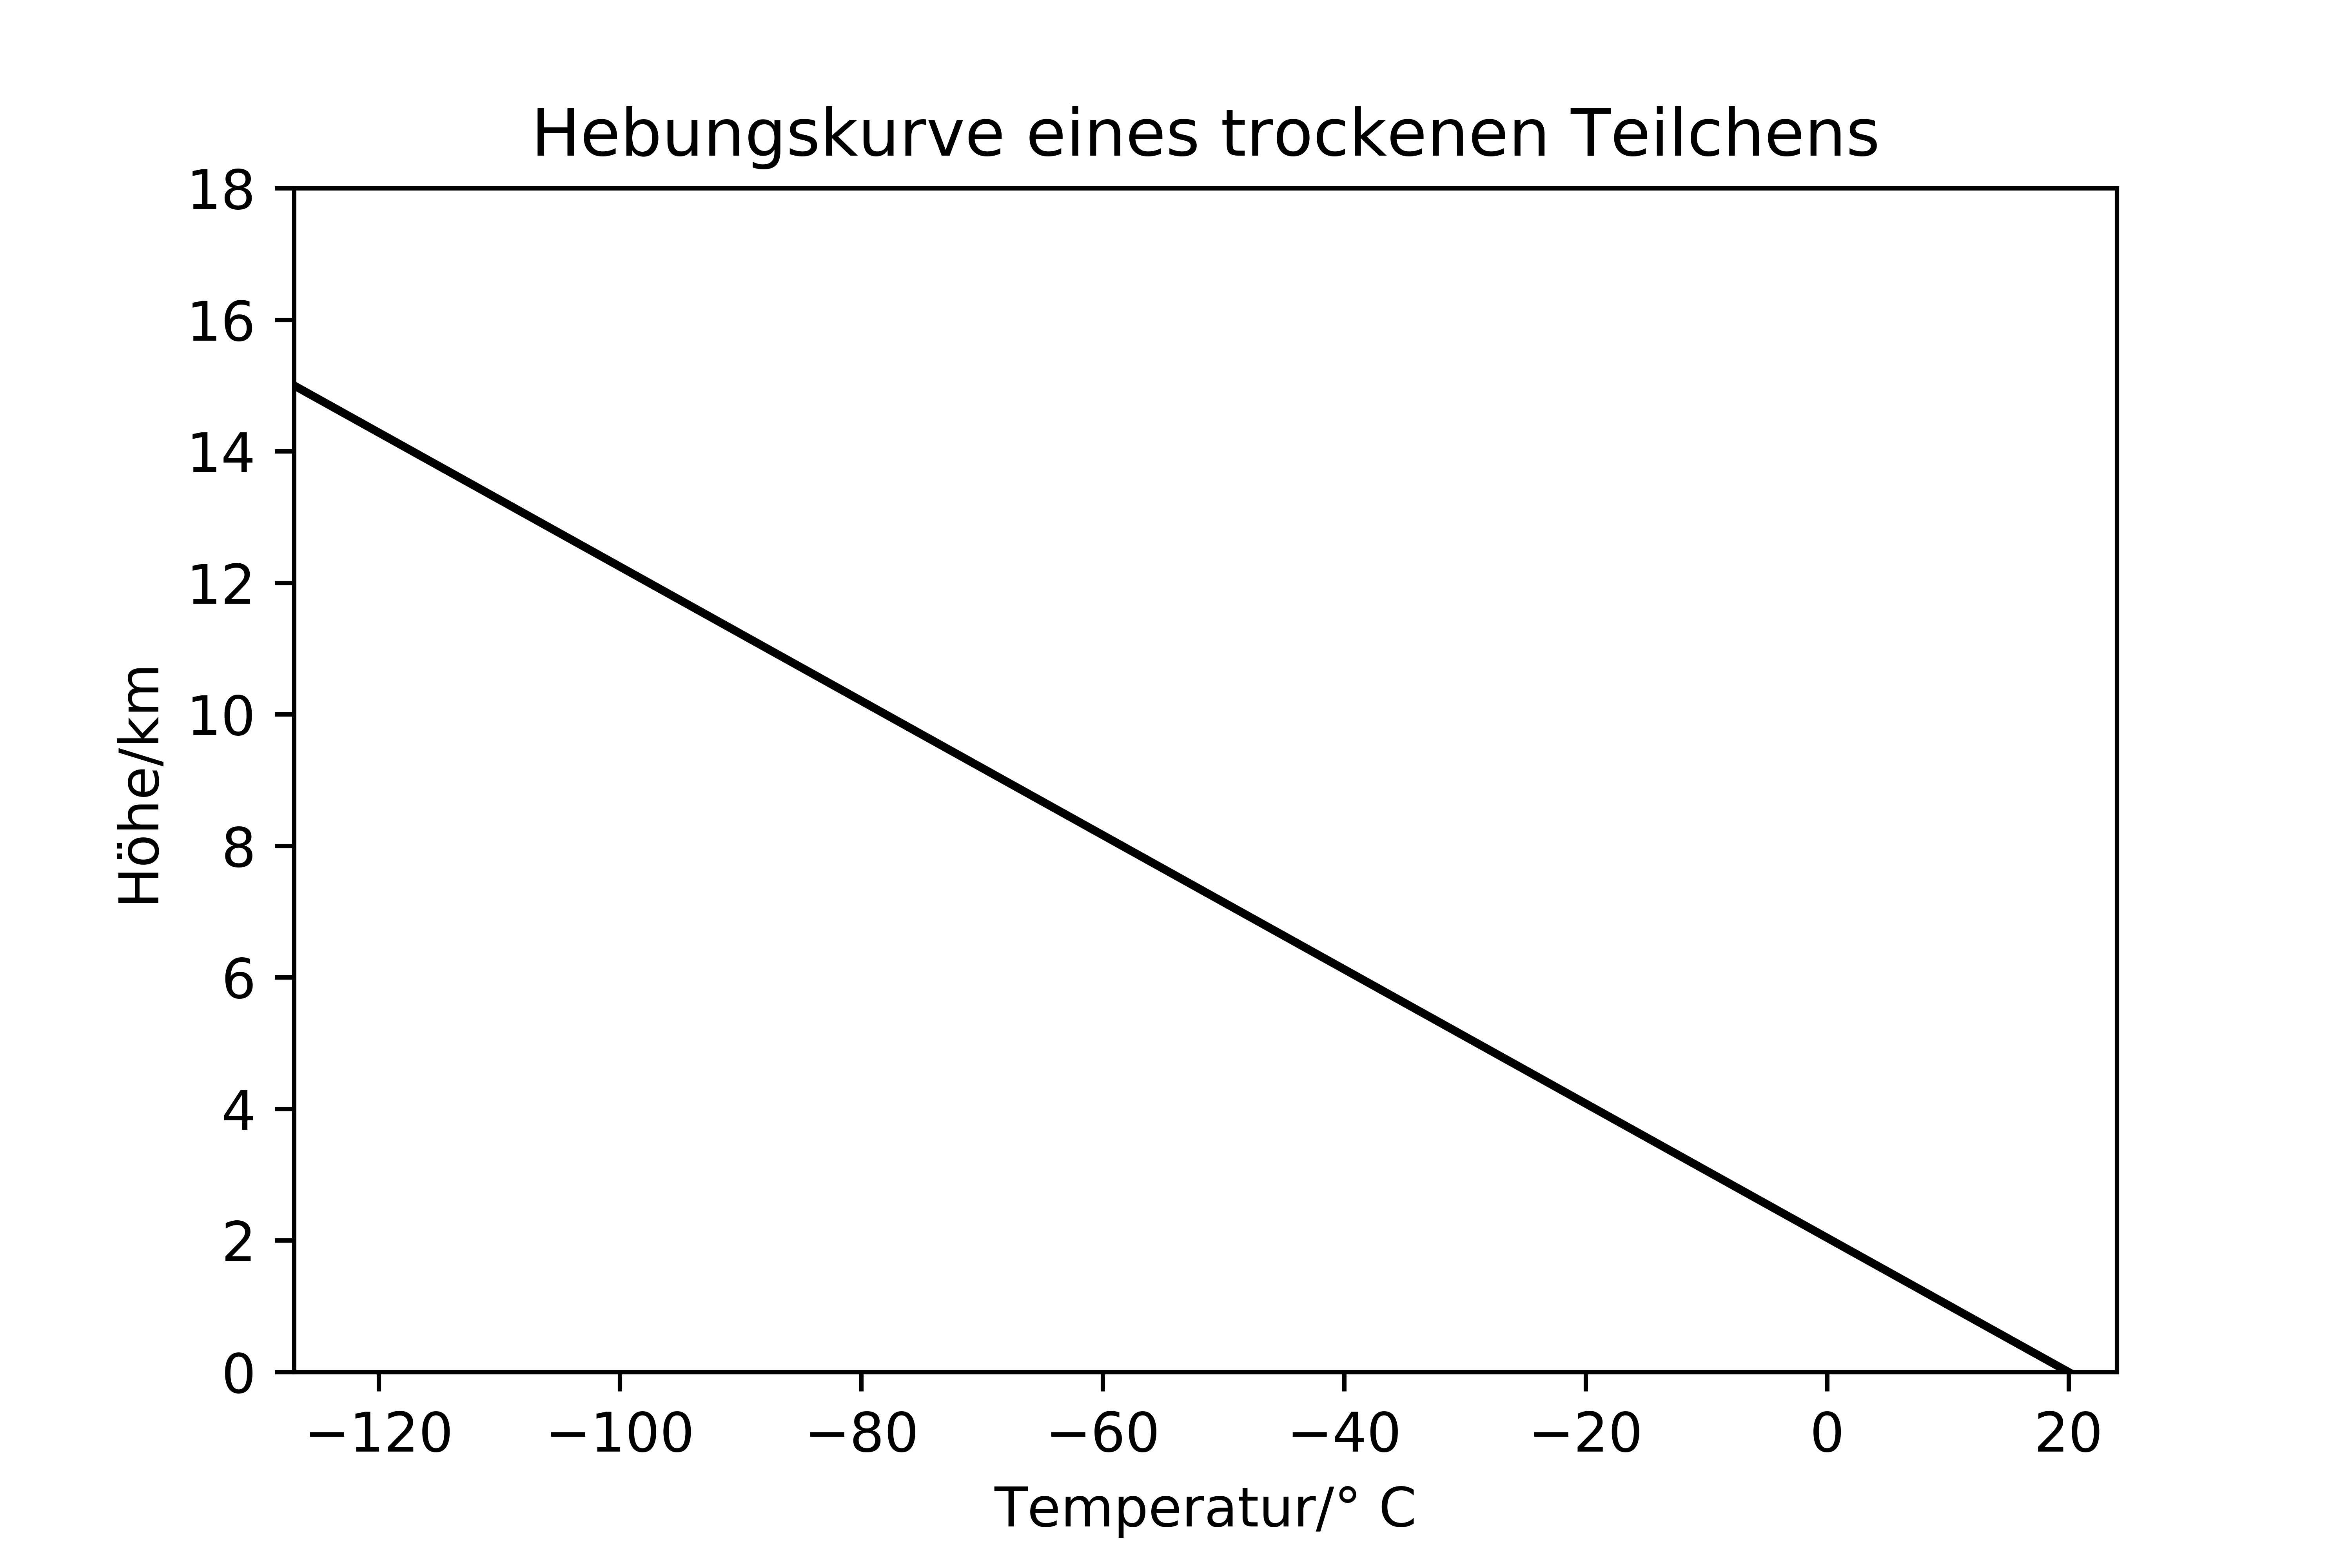
\includegraphics[width = .6\textwidth]{figs/lifting_dry.png}
\caption{Die adiabatische Hebung eines trockenen Luftteilchens, diese Kurve bezeichnet man auch als Hebungskurve\index{Hebungskurve}.}
\label{fig:trocken_hebung}
\end{center}
\end{figure}

Der trockenadiabatische Temperaturgradient ist kein Temperaturgradient im eigentlichen Sinne, er ist die Ableitung der Funktion $T = T(z)$, die die adiabatische Hebung eines Teilchens beschreibt. Diese Funktion nennt man auch Trockenadiabate\index{Trockenadiabate}. Er ist nicht die Vertikalkomponente des atmosphärischen Temperaturgradienten $\nabla T$. Diese muss überhaupt nicht, auch nicht näherungsweise, mit der Trockenadiabaten übereinstimmen. Es gilt nämlich
%
\begin{align}
\frac{\partial T}{\partial z} & = \theta\frac{\partial p}{\partial z}\frac{R_s}{c^{(p)}}\frac{1}{p_0}\left(\frac{p}{p_0}\right)^{\frac{R_s}{c^{(p)}} - 1} + \frac{\partial\theta}{\partial z}\left(\frac{p}{p_0}\right)^{\frac{R_s}{c^{(p)}}} = -\frac{g}{c^{(p)}} - g\frac{p}{R_sT}\frac{\partial\theta}{\partial p}\left(\frac{p}{p_0}\right)^{\frac{R_s}{c^{(p)}}}\nonumber\\
\Rightarrow g\frac{p}{R_s\theta}\frac{\partial\theta}{\partial p} & = -\left(\Gamma_d - \Gamma\right), \label{eq:vert_temp_gradient}
\end{align}
%
mit
%
\begin{align}
\Gamma \coloneqq -\frac{\partial T}{\partial z}.
\end{align}

Die materielle Ableitung von Glg. \eqref{eq:pot_temp} ist
%
\begin{align}
\md{T} & = \md{\theta}\left(\frac{p}{p_0}\right)^{R_s/c^{(p)}} + \theta\frac{dp}{dt}\frac{1}{p_0}\frac{R_s}{c^{(p)}}\left(\frac{p}{p_0}\right)^{R_s/c^{(p)} - 1} = \frac{T}{\theta}\md{\theta} + \frac{T}{p}\omega\frac{R_s}{c^{(p)}} = \frac{T}{\theta}\md{\theta} + \frac{\omega}{\rho c^{(p)}}.
\end{align}
%
Hieraus folgt
%
\begin{align}
c^{(v)}\frac{T}{\theta}\md{\theta} + \frac{T}{p}\omega\frac{R_s}{c^{(p)}}c^{(v)} + p\md{}\frac{R_sT}{p} & = \frac{q_T^{(V)}}{\rho} - \frac{sT}{\rho}q_\rho^{(V)}\nonumber\\
\Leftrightarrow \md{\theta}\frac{T}{\theta} + \frac{\omega T}{p}\frac{R_s}{c^{(p)}} - \frac{R_sT}{pc^{(v)}}\omega + \frac{R_s}{c^{(v)}}\md{T} & = \frac{q_T^{(V)}}{c^{(v)}\rho} - \frac{sT}{c^{(v)}\rho}q_\rho^{(V)}\nonumber\\
\Leftrightarrow \frac{T}{\theta}\md{\theta} + \frac{\omega R_sT}{p}\left(\frac{1}{c^{(p)}} - \frac{1}{c^{(v)}}\right)\nonumber\\
+ \frac{R_s}{c^{(v)}}\left(\frac{T}{\theta}\md{\theta} + \frac{T}{p}\omega\frac{R_s}{c^{(p)}}\right) & = \frac{q_T^{(V)}}{c^{(v)}\rho} - \frac{sT}{c^{(v)}\rho}q_\rho^{(V)}\nonumber\\
\Leftrightarrow \frac{T}{\theta}\md{\theta}\frac{c^{(p)}}{c^{(v)}} + \frac{\omega R_sT}{p}\frac{c^{(v)} - c^{(p)} + R_s}{c^{(v)}c^{(p)}} & = \frac{q_T^{(V)}}{c^{(v)}\rho} - \frac{sT}{c^{(v)}\rho}q_\rho^{(V)}.
\end{align}
%
Damit lautet Erste Hauptsatz für Thermodynamik für ein Gas in Termen der potentiellen Temperatur
%
\begin{center}
\doublebox{\parbox{0.8\textwidth}{
\begin{center}
\begin{align}
\md{\theta} = \frac{\theta}{T\rho c^{(p)}}\left(q_T^{(V)} - sTq_\rho^{(V)}\right).\label{eq:td1_dry_pot}
\end{align}
\end{center}
}}
\end{center}
%
Multipliziert man diese Gleichung mit $\rho$, erhält man
%
\begin{align}
\rho\frac{\partial\theta}{\partial t} + \rho\mathbf{v}\cdot\nabla\theta = \frac{\theta}{Tc^{(p)}}\left(q_T^{(V)} - sTq_\rho^{(V)}\right).
\end{align}
%
Addiert man das Produkt der potentiellen Temperatur\index{potentielle Temperatur}\index{Temperatur!potentielle} mit der Kontinuitätsgleichung
%
\begin{align}
\theta\frac{\partial\rho}{\partial t} + \theta\mathbf{v}\cdot\nabla\rho + \theta\rho\nabla\cdot\mathbf{v} = \theta q_\rho^{(V)} = \frac{\theta}{Tc^{(p)}}Tc^{(p)}q_\rho^{(V)}
\end{align}
%
hinzu, folgt
%
\begin{center}
\doublebox{\parbox{0.8\textwidth}{
\begin{center}
\begin{align}
\frac{\partial\left(\rho\theta\right)}{\partial t} + \nabla\cdot\left(\rho\theta\mathbf{v}\right) = \frac{\theta}{Tc^{(p)}}\left(q_T^{(V)} + T\left(c^{(p)} - s\right)q_\rho^{(V)}\right).\label{eq:td1_id_gas_pot_mod}
\end{align}
\end{center}
}}
\end{center}
%
Diese Form bezeichnet man auch als \textit{Flussform}\index{Flussform}, wohingegen Glg. \eqref{eq:td1_dry_pot} \textit{Advektionsform}\index{Advektionsform} hat. Die Flussform lässt sich als eine formale Kontinuitätsgleichung verstehen.

\subsection{Druck als prognostische Variable}
\label{sec:druck_als_prognostische_variable}

Nun soll noch die Definition der potentiellen Temperatur in die Zustandsgleichung eingesetzt werden:
%
\begin{align}
p & = \rho R_s\theta\left(\frac{p}{p_0}\right)^{R_s/c^{(p)}}\Rightarrow p^{1 - R_s/c^{(p)}} = \rho R_s\theta\frac{1}{p_0^{R_s/c^{(p)}}}\label{eq:state_theta_deriv_0}\\
\Rightarrow p^{1/\kappa} & = \rho R_s\theta\frac{1}{p_0^{R_s/c^{(p)}}}\Rightarrow p = \left(\rho R_s\theta\right)^\kappa\left(\frac{1}{p_0}\right)^{\kappa - 1}\label{eq:state_theta}
\end{align}
%
Auch für $p$ kann eine prognostiosche Gleichung\index{prognostische Gleichung!Druck}\index{Druck!prognostische Gleichung}\index{Druck!Gleichung!prognostische}\index{Gleichung!prognostische!Druck} hergeleitet werden:
%
\begin{align}
p & = \rho R_sT \Rightarrow \md{p} = R_s\left(T\md{\rho} + \rho\md{T}\right)
\end{align}
%
Mit
%
\begin{align}
\md{\rho} = -\rho\nabla\cdot\mathbf{v} + q_\rho^{(V)}, && \md{T} = \frac{T}{\theta}\md{\theta} + \frac{TR_s}{c^{(p)}p}\md{p}
\end{align}
%
folgt
%
\begin{align}
\md{p} & = R_sT\left(-\rho\nabla\cdot\mathbf{v} + q_{\rho}\right) + R_s\rho\left(\frac{T}{\theta}\md{\theta} + \frac{TR_s}{c^{(p)}p}\md{p}\right)\nonumber\\
& = -p\nabla\cdot\mathbf{v} + R_sTq_\rho^{(V)} + \frac{p}{\theta}\md{\theta} + \frac{R_s}{c^{(p)}}\md{p}\nonumber\\
\Leftrightarrow \frac{c^{(v)}}{c^{(p)}}\md{p} & = -p\nabla\cdot\mathbf{v} + R_sTq_\rho^{(V)} + \frac{p}{\theta}\md{\theta}\nonumber\\
\Leftrightarrow \frac{\partial p}{\partial t} & = -\mathbf{v}\cdot\nabla p - \frac{c^{(p)}}{c^{(v)}}p\nabla\cdot\mathbf{v} + \frac{c^{(p)}}{c^{(v)}}R_sTq_\rho^{(V)} + \frac{p}{T\rho c^{(v)}}\left(q_T^{(V)} - sTq_\rho^{(V)}\right)
\end{align}
%
\begin{center}
\doublebox{\parbox{0.8\textwidth}{
\begin{center}
\begin{align}
\Leftrightarrow \frac{\partial p}{\partial t} = -\mathbf{v}\cdot\nabla p - \frac{c^{(p)}}{c^{(v)}}p\nabla\cdot\mathbf{v} + \frac{c^{(p)}}{c^{(v)}}R_sTq_\rho^{(V)} + \frac{R_s}{c^{(v)}}\left(q_T^{(V)} - sTq_\rho^{(V)}\right).\label{eq:pressure_prognostic_equation}
\end{align}
\end{center}
}}
\end{center}

\subsubsection{Exner-Druck als prognostische Variable}
\label{sec:exner-druck_als_prognostische_variable}

Definiert man den \textit{Exner-Druck}\index{Exner-Druck} $\Pi$ durch
%
\begin{align}
\Pi \coloneqq \frac{T}{\theta} = \left(\frac{p}{p_0}\right)^{R_s/c^{(p)}} \Leftrightarrow p = \Pi^{c^{(p)}/R_s}p_0,\label{eq:def_exner-druck}
\end{align}
%
gilt der Zusammenhang
%
\begin{align}
p & = \rho R_s\theta\Pi \Leftrightarrow \Pi^{c^{(p)}/R_s} = \frac{\rho R_s\theta}{p_0}\Pi \Leftrightarrow \Pi^{c^{(v)}/R_s} = \frac{\rho R_s\theta}{p_0}\nonumber\\
\Pi & = \left(\frac{\rho R_s\theta}{p_0}\right)^{R_s/c^{(v)}}.\label{eq:exner_pressure_diag}
\end{align}
%
Hieraus folgt
%
\begin{align}
\nabla p = R_s \theta\rho\nabla\Pi + R_s\Pi\nabla\left(\rho\theta\right) = c^{(p)}\theta\rho\nabla\Pi - c^{(v)}\theta\rho\nabla\Pi + R_s\Pi\nabla\left(\rho\theta\right).
\end{align}
%
Man stellt fest:
%
\begin{align}
-c^{(v)}\theta\rho\nabla\Pi + R_s\Pi\nabla\left(\rho\theta\right) & = -\left(\frac{R_s}{p_0}\right)^{R_s/c^{(v)}}c^{(v)}\theta\rho\nabla\left(\rho\theta\right)^{R_s/c^{(v)}} + R_s\Pi\nabla\left(\rho\theta\right)\nonumber\\
&\stackrel{\text{Glg. }\eqref{eq:exner_pressure_diag}}{=} R_s\left(\Pi - \left(\frac{R_s}{p_0}\right)^{R_s/c^{(v)}}\left(\rho\theta\right)^{R_s/c^{(v)}}\right)\nabla\left(\rho\theta\right) = 0
\end{align}
%
Somit kann man für die Druckgradientbeschleunigung\index{Druckgradientbeschleunigung!Exner-Druck}\index{Exner-Druck!Druckgradientbeschleunigung} schreiben
%
\begin{align}
-\frac{1}{\rho}\nabla p = -c^{(p)}\theta\nabla\Pi.\label{eq:exner_pressure_gradient_acc}
\end{align}
%
Mit Glg. \eqref{eq:diff_op_rule_3} folgt
%
\begin{align}
\nabla\cdot\left(\rho c^{(p)}\Pi\theta\mathbf{v}\right) & = \rho c^{(p)}\theta\mathbf{v}\cdot\nabla\Pi + \Pi\nabla\cdot\left(\rho c^{(p)}\theta\mathbf{v}\right)\nonumber\\
\Leftrightarrow -\rho\mathbf{v}\cdot c^{(p)}\theta\nabla\Pi & = -\nabla\cdot\left(\rho c^{(p)}T\mathbf{v}\right) +  c^{(p)}\Pi\nabla\cdot\left(\rho\theta\mathbf{v}\right)\nonumber\\
\Leftrightarrow -\rho\mathbf{v}\cdot c^{(p)}\theta\nabla\Pi & = -\nabla\cdot\left(\rho h\mathbf{v}\right) + c^{(p)}\Pi\nabla\cdot\left(\rho\theta\mathbf{v}\right)\
\end{align}
%
mit der spezifischen Enthalpie $h$. Hieraus kann man ablsesen:
%
\begin{itemize}
\item Wirkt der Druckgradient beschleunigend, so divergiert der Fluss der potentiellen Temperatur stärker als der Fluss der Enthalpie.
\item Wirk der Druckgradient bremsend, so divergiert der Fluss der Enthalpie stärker als der Fluss der potentiellen Temperatur.
\end{itemize}
%
Nun werden noch zwei prognostische Gleichungen für $\Pi$ hergeleitet. Die lokalzeitliche Ableitung von Glg. \eqref{eq:exner_pressure_diag} lautet im adiabatischen Fall
%
\begin{align}
\frac{\partial\Pi}{\partial t} & = \frac{R_s}{c^{(v)}}\left(\frac{\rho R_s\theta}{p_0}\right)^{\frac{R_s}{c^{(v)}} - 1}\frac{\rho R_s\theta}{p_0}\left(\frac{1}{\theta}\frac{\partial\theta}{\partial t} + \frac{1}{\rho}\frac{\partial\rho}{\partial t}\right) = \frac{R_s}{c^{(v)}\theta\rho}\left(\frac{\rho R_s\theta}{p_0}\right)^{\frac{R_s}{c^{(v)}}}\left(\rho\frac{\partial\theta}{\partial t} + \theta\frac{\partial\rho}{\partial t}\right)\nonumber\\
& = \frac{R_s\Pi}{c^{(v)}\theta\rho}\left(\rho\frac{\partial\theta}{\partial t} + \theta\frac{\partial\rho}{\partial t}\right) = \frac{R_s\Pi}{c^{(v)}\theta\rho}\left(-\rho\mathbf{v}\cdot\nabla\theta - \theta\nabla\cdot\left(\rho\mathbf{v}\right)\right) = -\frac{R_s\Pi}{c^{(v)}\theta\rho}\nabla\cdot\left(\rho\theta\mathbf{v}\right).
\end{align}
%
Fügt man die diabatischen Terme hinzu, folgt
%
\begin{center}
\doublebox{\parbox{0.8\textwidth}{
\begin{center}
\begin{align}
\frac{\partial\Pi}{\partial t} & = -\frac{R_s\Pi}{c^{(v)}\theta\rho}\left[\nabla\cdot\left(\rho\theta\mathbf{v}\right) - \frac{\theta}{Tc^{(p)}}\left(q_T^{(V)} + T\left(c^{(p)} - s\right)q_\rho^{(V)}\right)\right].\label{eq:def_exner-pressure_local_derivative}
\end{align}
\end{center}
}}
\end{center}
%
Für die materielle Ableitung von Glg. \eqref{eq:exner_pressure_diag} erhält man
%
\begin{align}
\md{\Pi} = \frac{R_s}{c^{(v)}}\left(\frac{\rho R_s\theta}{p_0}\right)^{R_s/c^{(v)} - 1}\frac{R_s}{p_0}\md{\left(\rho\theta\right)} = \frac{R_s}{c^{(v)}\rho\theta}\left(\frac{\rho R_s\theta}{p_0}\right)^{R_s/c^{(v)}}\md{\left(\rho\theta\right)} = \frac{R_s\Pi}{c^{(v)}\rho\theta}\md{\left(\rho\theta\right)}.
\end{align}
%
Mit Glg. \eqref{eq:td1_id_gas_pot_mod} folgt
%
\begin{center}
\doublebox{\parbox{0.8\textwidth}{
\begin{center}
\begin{align}
\md{\Pi} = \frac{R_s\Pi}{c^{(v)}}\left[-\nabla\cdot\mathbf{v} + \frac{1}{\rho Tc^{(p)}}\left(q_T^{(V)} + T\left(c^{(p)} - s\right)q_\rho^{(V)}\right)\right].\label{eq:exner-pressure_material_derivative}
\end{align}
\end{center}
}}
\end{center}

\subsection{Entropie als prognostische Variable}
\label{sec:entropie_als_prognostische_variable}

Setzt man die Zustandsgleichungen Glg.en \eqref{eq:kalorisch_id_gase} und \eqref{eq:zustand_ideal} in Glg. \eqref{eq:sackur-tetrode-equation} ein, folgt unter Vernachlässigung des Ungefähr-Zeichens
%
\begin{align}
S\left(E, V, N\right) & = k_B\frac{3N}{2}\ln\left(c\right) + k_BN\ln\left(\frac{V}{N}\right) + k_B\frac{3N}{2}\ln\left(\frac{E}{N}\right)\nonumber\\
& = k_B\frac{3N}{2}\ln\left(c\right) + k_BN\ln\left(\frac{k_BT}{p}\right) + k_B\frac{3N}{2}\ln\left(\frac{3}{2}k_BT\right)\nonumber\\
& = k_BN\ln\left(k_BT\right) + k_B\frac{3N}{2}\ln\left(\frac{3}{2}k_BT\right) - Nk_B\ln\left(p\right) + k_B\frac{3N}{2}\ln\left(c\right)\nonumber\\
& = k_B\frac{5N}{2}\ln\left(k_BT\right) + k_B\frac{3N}{2}\ln\left(\frac{3}{2}\right) - Nk_B\ln\left(p\right) + k_B\frac{3N}{2}\ln\left(c\right)\nonumber\\
& = k_B\frac{5N}{2}\ln\left(T\right) - Nk_B\ln\left(p\right) + k_B\frac{5N}{2}\ln\left(k_B\right) + k_B\frac{3N}{2}\ln\left(\frac{3}{2}\right) + k_B\frac{3N}{2}\ln\left(c\right)\nonumber\\
& = k_B\frac{5N}{2}\ln\left(T\right) - Nk_B\ln\left(p\right) + Nk_B\ln\left(k_B^{\frac{5}{2}}\right) + Nk_B\ln\left[\left(\frac{3}{2}\right)^\frac{3}{2}\right] + Nk_B\ln\left(c^\frac{3}{2}\right)\nonumber\\
& = k_B\frac{5N}{2}\ln\left(T\right) - Nk_B\ln\left(p\right) + Nk_B\ln\left[k_B^{\frac{5}{2}}\left(\frac{3}{2}\right)^\frac{3}{2}c^\frac{3}{2}\right]\nonumber\\
& = k_B\frac{5N}{2}\ln\left(T\right) - Nk_B\ln\left(p\right) + Nk_B\ln\left[\left(\frac{3k_B}{2}c\right)^\frac{3}{2}k_B\right].\label{eq:entropy_id_gas_deriv_0}
\end{align}
%
Aus Glg. \eqref{eq:def_id_gas_entropy_constant} weiß man
%
\begin{align}
c = \frac{Me^{5/3}}{3\pi\hbar^2},
\end{align}
%
wobei $M$ die Masse der Teilchen bezeichnet. Hieraus folgt
%
\begin{align}
S\left(E, V, N\right) & = k_B\frac{5N}{2}\ln\left(T\right) - Nk_B\ln\left(p\right) + Nk_B\ln\left[\left(\frac{3k_B}{2}\frac{Me^{5/3}}{3\pi\hbar^2}\right)^\frac{3}{2}k_B\right]\nonumber\\
& = k_B\frac{5N}{2}\ln\left(T\right) - Nk_B\ln\left(p\right) + Nk_B\ln\left[\left(\frac{Me^{5/3}k_B}{2\pi\hbar^2}\right)^\frac{3}{2}k_B\right].
\end{align}
%
Mit
%
\begin{align}
c' \coloneqq k_B\ln\left[\left(\frac{Me^{5/3}k_B}{2\pi\hbar^2}\right)^\frac{3}{2}k_B\right]
\end{align}
%
kann man abkürzend
%
\begin{align}
S\left(E, V, N\right) & = k_B\frac{5N}{2}\ln\left(T\right) - Nk_B\ln\left(p\right) + Nc'
\end{align}
%
notieren. Somit erhält man
%
\begin{align}
S\left(E, V, N\right) & = C^{(p)}\ln\left(T\right) - Nk_B\ln\left(p\right) + Nc'\nonumber\\
& = C^{(p)}\ln\left[\theta\left(\frac{p}{p_0}\right)^{\frac{R_s}{c^{(p)}}}\right] - Nk_B\ln\left(p\right) + Nc'\nonumber\\
& = C^{(p)}\ln\left(\theta\right) + R_sm\ln\left(\frac{p}{p_0}\right) - Nk_B\ln\left(p\right) + Nc'\nonumber\\
& = C^{(p)}\ln\left(\theta\right) + k_BN\ln\left(p\right) - Nk_B\ln\left(p\right) - Nk_B\ln\left(p_0\right) + Nc'\nonumber\\
& = C^{(p)}\ln\left(\theta\right) - Nk_B\ln\left(p_0\right) + Nk_B\ln\left[\left(\frac{k_BMe^{5/3}}{2\pi\hbar^2}\right)^\frac{3}{2}k_B\right]\nonumber\\
& = C^{(p)}\ln\left(\theta\right) + Nk_B\ln\left[\frac{k_B}{p_0}\left(\frac{k_BMe^{5/3}}{2\pi\hbar^2}\right)^\frac{3}{2}\right] = C^{(p)}\ln\left(\theta\right) + \frac{2C^{(p)}}{5}\ln\left[\frac{k_B}{p_0}\left(\frac{k_BMe^{5/3}}{2\pi\hbar^2}\right)^\frac{3}{2}\right]\nonumber\\
& = C^{(p)}\ln\left(\theta\right) + mc''.
\end{align}
%
Mit
%
\begin{align}
c'' \coloneqq \frac{2c^{(p)}}{5}\ln\left[\frac{k_B}{p_0}\left(\frac{k_BMe^{5/3}}{2\pi\hbar^2}\right)^\frac{3}{2}\right].
\end{align}
%
Für die spezifische Entropie $s$ gilt somit
%
\begin{align}
s = c^{(p)}\ln\left(\theta\right) + c''\label{eq:entropy_spec_id_gas}
\end{align}
%
mit der molaren Masse $M$.
%
Man kann auch $s$ als Zustandsgröße verwenden. Es gilt nämlich
%
\begin{center}
\doublebox{\parbox{0.8\textwidth}{
\begin{center}
\begin{align}
\rho\md{s} = c^{(p)}\frac{\rho}{\theta}\md\theta = \frac{1}{T}\left(q_T^{(V)} - sTq_\rho^{(V)}\right).
\end{align}
\end{center}
}}
\end{center}
%
Addiert man das Produkt der Entropie $s$ mit der Kontinuitätsgleichung
%
\begin{align}
s\frac{\partial\rho}{\partial t} + s\mathbf{v}\cdot\nabla\rho + s\rho\nabla\cdot\mathbf{v} = sq_\rho^{(V)}
\end{align}
%
hinzu, folgt mit der Definition
%
\begin{align}
\newtilde{s} \coloneqq \rho s.\label{eq:def_entropy_density}
\end{align}
%
die Gleichung
%
\begin{center}
\doublebox{\parbox{0.8\textwidth}{
\begin{center}
\begin{align}
\Rightarrow \frac{\partial\newtilde{s}}{\partial t} + \nabla\cdot\left(\newtilde{s}\mathbf{v}\right) & = \frac{q_T^{(V)}}{T}.\label{eq:td_1_id_gas_density_entropy}
\end{align}
\end{center}
}}
\end{center}
%
Man mache sich an dieser Stelle klar, dass die Konstante $c''$ nicht irrelevant ist. Ersetze nämlich
%
\begin{align}
s \to s - \newtilde{c}
\end{align}
%
mit einer beliebigen Konstante $\newtilde{c}$, dann wird aus Glg. \eqref{eq:td_1_id_gas_density_entropy}
%
\begin{align}
\frac{\partial\newtilde{s}}{\partial t} + \nabla\cdot\left(\newtilde{s}\mathbf{v}\right) & = \frac{q_T^{(V)}}{T} + \newtilde{c}q_\rho^{(V)}.
\end{align}
%
Möchte man $c''$ also loswerden, möchte man also $c^{(p)}\ln\left(\theta\right)$ direkt als Ausdruck für die Entropie verwenden, so geht dies nur unter Vernachlässigung von Massenquelltermen. Diese tragen nicht zur Evolution der Entropiedichte bei.

Mit der Bezeichnungsänderung
%
\begin{align}
c \to \frac{c''}{M}
\end{align}
%
ergibt sich als Diagnostik für die potentielle Temperatur
%
\begin{align}
\theta = \exp\left(\frac{s - c}{c^{(p)}}\right) = \exp\left(\frac{\frac{\newtilde{s}}{\rho} - c}{c^{(p)}}\right) = \exp\left(-\frac{c}{c^{(p)}}\right)\exp\left(\frac{\newtilde{s}}{c^{(p)}\rho}\right).\label{eq:pot_temp_entropy_diagnostics}
\end{align}
%
Mit
%
\begin{align}
\theta = T\left(\frac{p_0}{p}\right)^{R_s/c^{(p)}} = T\left(\frac{p_0}{\rho R_sT}\right)^{R_s/c^{(p)}} = \left(\frac{p_0}{R_s}\right)^{R_s/c^{(p)}}T^{c^{(v)}/c^{(p)}}\rho^{-R_s/c^{(p)}}
\end{align}
%
erhält man weiter
%
\begin{align}
T = \left(\frac{R_s}{p_0}\right)^{R_s/c^{(v)}}\exp\left(-\frac{c}{c^{(v)}}\right)\rho^{R_s/c^{(v)}}\exp\left(\frac{\newtilde{s}}{c^{(v)}\rho}\right).
\end{align}
%
Mit
%
\begin{align}
\beta \coloneqq \left(\frac{R_s}{p_0}\right)^{R_s/c^{(v)}}\exp\left(-\frac{c}{c^{(v)}}\right)
\end{align}
%
kann man dies kürzer als
%
\begin{center}
\doublebox{\parbox{0.8\textwidth}{
\begin{center}
\begin{align}
T = \beta\rho^{R_s/c^{(v)}}\exp\left(\frac{\newtilde{s}}{c^{(v)}\rho}\right)
\end{align}
\end{center}
}}
\end{center}
%
notieren. Dies ist die Zustandsgleichung idealer Gase in Entropieformulierung\index{Zustandsgleichung idealer Gase!Entropieformulierung}.

\section{Ideales Gasgemisch mit homogener Zusammensetzung}
\label{sec:ideales_gasgemisch_mit_homogener_zusammensetzung}

N-atomige ideale Gase haben gegenüber dem einatomigen Gas zusätzlich Rotations- und Vibrationsfreiheitsgrade. Diese zusätzlichen Freiheitsgrade erhöhen die Wärmekapazitäten und ein analytischer Ausdruck für die Entropie liegt dann nicht mehr vor. Als Modell für dieses komplexe System wird ein einatomiges ideales Gas mit der gleichen mittleren molaren Masse wie das Originalgas verwendet, wobei für die Wärmekapazitäten Messweret oder Produkte einer fundamentaleren Theorie verwendet. Damit lassen sich die im vorigen Abschnitt aufgeführten Ergebnisse insbesondere auch auf trockene übertragen.

\section{Ideales Gasgemisch mit variabler Zusammensetzung}
\label{sec:ideales_gasgemisch_mit_variabler_zusammensetzung}

Hier geht man von einem Gasgemisch aus $N \geq 1$ idealen einatomigen Gasen aus. Glg. \eqref{eq:td_1_id_gas_density_entropy} lässt sich auf jede dieser Komponenten anwenden und überlagern. Dabei gilt
%
\begin{align}
\newtilde{s}_i = s_i\rho_i
\end{align}
%
für $1 \leq i \leq N$ und
%
\begin{align}
s = \sum_{i = 1}^N\newtilde{s}_i.
\end{align}
%
Prinzipiell bekommt jede Gassorte ihren eigenen Temperatur-Quellterm $q_{T, i}$. Man nimmt jedoch vereinfachend an, dass der anschließende Austausch der Energie zwischen den Gassorten so schnell ist, dass man sie als instantan annehmen kann. In diesem Fall kann man
%
\begin{align}
q_{T, i}^{(V)} = \frac{\rho_i}{\rho}q_T^{(V)}
\end{align}
%
Somit gilt Glg. \eqref{eq:td_1_id_gas_density_entropy}
%
\begin{center}
\doublebox{\parbox{0.8\textwidth}{
\begin{center}
\begin{align}
\Rightarrow \frac{\partial\newtilde{s}}{\partial t} + \nabla\cdot\left(\newtilde{s}\mathbf{v}\right) & = \frac{q_T^{(V)}}{T}\label{eq:td_1_2_entropy_id_gas}
\end{align}
\end{center}
}}
\end{center}
%
auch mit diesen Definitionen.

\subsection{Beispiel: feuchte Luft}
\label{sec:beispiel:_feuchte_luft}

Hier soll es zunächst um feuchte Luft\index{feuchte Luft}\index{Luft!feuchte} unter Abwesenheit von Kondensaten gehen. In solch einem System gilt
%
\begin{align}
s = \rho_d\left[c_d^{(p)}\ln\left(\theta\right) + \frac{1}{\newtilde{M}_d}\newtilde{c}_d''\right] + \rho_v\left[c_v^{(p)}\ln\left(\theta_v\right) + \frac{1}{\newtilde{M}_v}\newtilde{c}_v''\right],
\end{align}
%
wobei $\theta_v \coloneqq T\left(\frac{p_0}{p}\right)^{R_v/c_v^{(p)}}$ die potentielle Temperatur von Wasserdampf\index{Wasserdampf!potentielle Temperatur}\index{potentielle Temperatur!Wasserdampf} ist. In jeder individuellen Phase $i$ gilt
%
\begin{align}
\nabla p_i & = \rho_ic_i^{(p)}\nabla T - \rho_iT\nabla s_i.
\end{align}
%
Somit folgt für zwei Phasen $d, v$ durch Summation
%
\begin{align}
\nabla p  = \nabla\left(p_d + p_v\right) & = \rho_dc_d^{(p)}\nabla T - \rho_dT\nabla s_d + \rho_vc_v^{(p)}\nabla T - \rho_vT\nabla s_v.
\end{align}
%
Hieraus folgt
%
\begin{align}
\Leftrightarrow -\frac{1}{\rho}\nabla p & = -c_h^{(p)}\nabla T + \frac{T}{\rho}\left(\rho_d\nabla s_d + \rho_v\nabla s_v\right)\label{eq:pressure_grad_sup_deriv_0}
\end{align}
%
mit der isobaren spezifischen Wärmekapazität feuchter Luft\index{spezifische Wärmekapazität!feuchter Luft}\index{feuchter Luft!spezifische Wärmekapazität}
%
\begin{align}
c_h^{(p)} = \frac{\rho_dc_d^{(p)} + \rho_vc_v^{(p)}}{\rho = \rho_d + \rho_v}.
\end{align}
%
Glg. \eqref{eq:pressure_grad_sup_deriv_0} kann man auf ein Gemisch von $N \geq 1$ idealen Gasen verallgemeinern:
%
\begin{center}
\doublebox{\parbox{0.8\textwidth}{
\begin{center}
\begin{align}
\Leftrightarrow -\frac{1}{\rho}\nabla p & = -c_g^{(p)}\nabla T + \frac{T}{\rho}\sum_{i = 1}^{N}\rho_i\nabla s_i\label{eq:pressure_grad_sup}
\end{align}
\end{center}
}}
\end{center}
%
Hierbei bezieht sich der Index $g$ auf die Gasphase und es gelten
%
\begin{align}
\rho = \sum_{i = 1}^N\rho_i, && c_g^{(p)} = \frac{1}{\rho}\sum_{i = 1}^N\rho_ic_i^{(p)}.
\end{align}
%
Man definiert die sogenannte \textit{virtuelle potentielle Temperatur}\index{potentielle virtuelle Temperatur}\index{Temperatur!potentielle!virtuelle}\index{Temperatur!virtuelle!potentielle}
$\theta_v$ durch
%
\begin{align}
\theta_v \coloneqq T_v\left(\frac{p_0}{p}\right)^{R_d/c_d^{(p)}},
\end{align}
%
hierbei ist
%
\begin{align}
T_v = \left(1 - q + \frac{q}{\epsilon}\right)T
\end{align}
%
die in Glg. \eqref{eq:def_virtual_temperature} definierte virtuelle Temperatur\index{virtuelle Temperatur}\index{Temperatur!virtuelle}. Dies ist eher eine Behelfsgröße als die potentielle Temperatur feuchter Luft $\theta_v$, denn für diese würde
%
\begin{align}
\theta_h \coloneqq T\left(\frac{p_0}{p}\right)^{R_h/c_h^{(p)}}
\end{align}
%
gelten. Die virtuelle potentielle Temperatur\index{potentielle virtuelle Temperatur}\index{Temperatur!potentielle!virtuelle}\index{Temperatur!virtuelle!potentielle} ist diejenige potentielle Temperatur\index{potentielle Temperatur}\index{Temperatur!potentielle}, die trockene Luft\index{trockene Luft}\index{Luft!trockene} haben müsste, um nach adiabatischer Kompression auf den Referenzdruck $p_0$ die gleiche Dichte zu haben wie die betrachtete feuchte Luft.

\section{Thermodynamische Bedeutung der Wärmeleitung}
\label{sec:thermodynamische_bedeutung_der_wärmeleitung}\index{Thermodynamik!Wärmeleitung}\index{Wärmeleitung!thermodynamische Bedeutung}

Glg. \eqref{eq:td_1_2_entropy_id_gas}
%
\begin{align}
\frac{\partial\newtilde{s}}{\partial t} + \nabla\cdot\left(\newtilde{s}\mathbf{v}\right) & = \frac{q_T^{(V)}}{T}\label{eq:td_1_2_entropy_id_gas_repeat}
\end{align}
%
ist eine Kombination des Ersten und Zweiten Hauptsatzes der Thermodynamik. Für $q_T^{(V)}$ gilt unter Abwesenheit von Strahlung und Kondensaten
%
\begin{align}
q_T^{(V)} = -\nabla\cdot\mathbf{j}_q + \epsilon,
\end{align}
%
hierbei ist $\mathbf{j}_q$ die Wärmestromdichte durch Wärmeleitung\index{Wärmeleitung}. Laut Glg. \eqref{eq:heat_current_from_heat_conduction} gilt
%
\begin{align}
\mathbf{j}_q = -\rho c_d^{(v)}\kappa\nabla T.
\end{align}
%
Man kann nun rechnen
%
\begin{align}
\frac{\nabla\cdot\left(\rho\kappa\nabla T\right)}{T} = \nabla\cdot\frac{\rho c_d^{(v)}\kappa\nabla T}{T} + \frac{\rho c_d^{(v)}\kappa}{T^2}\left(\nabla T\right)^2 = -\nabla\cdot\frac{\mathbf{j}_q}{T} + \frac{\rho c_d^{(v)}\kappa}{T^2}\left(\nabla T\right)^2.
\end{align}
%
Setzt man dies in Glg. \eqref{eq:td_1_2_entropy_id_gas_repeat} ein und integriert global, erhält man
%
\begin{align}
\int_A\frac{\partial\newtilde{s}}{\partial t}d^3r &= \frac{d}{dt}\int_A\newtilde{s}d^3r = \int_A-\nabla\cdot\frac{\mathbf{j}_q}{T} + \frac{\rho c_d^{(v)}\kappa}{T^2}\left(\nabla T\right)^2d^3r = -\int_{\partial A}\frac{\mathbf{j}_q}{T}\cdot d\mathbf{n} + \int_A\frac{\rho c_d^{(v)}\kappa}{T^2}\left(\nabla T\right)^2d^3r.
\end{align}
%
Die Evolutionsgleichung der Gesamtentropie der Atmosphäre
%
\begin{align}
S = \int_A\newtilde{s}d^3r
\end{align}
%
lautet in diesem Fall also
%
\begin{center}
\doublebox{\parbox{0.8\textwidth}{
\begin{center}
\begin{align}
\frac{dS}{dt} = \underbrace{-\int_{\partial A}\frac{\mathbf{j}_q}{T}\cdot d\mathbf{n}}_{\substack{\text{Wechselwirkung mit} \\\text{der Umgebung}}} + \underbrace{\int_A\frac{\rho c_d^{(v)}\kappa}{T^2}\left(\nabla T\right)^2d^3r}_{\substack{\text{Entropieproduktion durch} \\\text{Wärmeleitung (nichtnegativ)}}} + \underbrace{\int_A\frac{\epsilon}{T}d^3r\text{.}}_{\substack{\text{Entropieproduktion durch} \\\text{Dissipation (nichtnegativ)}}}
\end{align}
\end{center}
}}
\end{center}
%
Durch interne Prozesse in einem idealen Gas mit Viskosität kann also nur Entropie produziert werden, wie es vom Zweiten Hauptsatz der Thermodynamik gefordert wird.

\section{Anwendungen}
\label{sec:anwendungen}

\subsection{Die isentrope trockene Atmosphäre}
\label{sec:die_isentrope_trockene_atmosphaere}

In einer isentropen Atmosphäre (Atmosphäre homogener spezifischer Entropie) ist nach Glg. \eqref{eq:entropy_spec_id_gas} auch die potentielle Temperatur homogen. Dies führt zu einer anderen Abhängigkeit des Drucks von der Höhe als im Fall der isothermen Atmosphäre. Ist $\Gamma_d > 0$ der trockenadiabatische Temperaturgradient, gilt für die Temperatur $T(z) = T_0 - \Gamma_d z$ mit $T_0 \coloneqq T(z = 0)$. Damit folgt
%
\begin{align}
\frac{\partial p}{\partial z} = -g\rho = -g\frac{p}{R_dT} = -\frac{g}{R_d}\frac{p}{T_0 - \Gamma_d z} = \frac{gp}{R_d(\Gamma_d z - T_0)}
\end{align}
%
als zu lösende Differenzialgleichung für $p = p(z)$. Macht man den Ansatz
%
\begin{align}
p(z) = C\exp\left[f(z)\right]
\end{align}
%
mit einer stetig-differenzierbaren Funktion $f = f(z)$ und einer Konstanten $C > 0$, so folgt
%
\begin{align}
\frac{\partial p}{\partial z} = \frac{\partial f}{\partial z}p, 
\end{align}
%
man erhält also für $f$
%
\begin{align}
\frac{\partial f}{\partial z} = \frac{g}{R_d\left(\Gamma_d z - T_0\right)}, 
\end{align}
%
dies ist gelöst für
%
\begin{align}
f = \frac{g}{R_d\Gamma_d}\ln\left(T_0 - \Gamma_d z\right).
\end{align}
%
Damit folgt für den Druck
%
\begin{align}
p(z) = C\exp\left(\frac{g}{R_d\Gamma_d}\ln\left(T_0 - \Gamma_d z\right)\right) = C\left(T_0 - \Gamma_d z\right)^{\frac{g}{R_d\Gamma_d}}, 
\end{align}
%
mit $p(0) = p_0$ folgt $C = \frac{p_0}{T_0^{\frac{g}{\Gamma_d R_d}}}$. Es gilt also
%
\begin{center}
\doublebox{\parbox{0.8\textwidth}{
\begin{center}
\begin{align}
p(z) = p_0\left(1 - \frac{\Gamma_d z}{T_0}\right)^{\frac{g}{R_d\Gamma_d}}\label{eq:isentrop_atmo}.
\end{align}
\end{center}
}}
\end{center}
%
In der Troposphäre ist eine mit der Höhe lineare Temperaturabnahme realistischer als Isothermie. Allerdings ist der trockenadiabatische Gradient klimatologisch zu extrem. Man nimmt als \textit{Standardatmosphäre}\index{Standardatmosphäre} eine Atmosphäre mit einer auf die Geopotentialfläche Null reduzierten Temperatur von $T_0 = 290$ K $ = 16, 85^\circ$ C an und einer bis in eine Höhe $H = 12$ km linearen Temperaturabnahme $k = 0, 65$ K/100m. Darüber geht man von Isothermie aus. Ersetzt man in der Formel der isentropen Atmosphäre \eqref{eq:isentrop_atmo} den trockenadiabatischen Gradienten $\Gamma_d$ durch $k$ und verwendet darüber die barometrische Höhenformel, so folgt
%
\begin{align}
p(z) & = \left\lbrace\begin{array}{c}
p_0\left(1 - \frac{kz}{T_0}\right)^\frac{g}{R_dk}, \:z < H\\
p(H)\exp\left(-g\frac{z - H}{R_dT_T}\right) , \:z\geq H
\end{array}\right.
\end{align}
%
mit $T_T \coloneqq T_0 - kH$ als Temperatur der Tropopause.

\begin{figure}
\centering
\begin{subfigure}[c]{.49\textwidth}
\centering
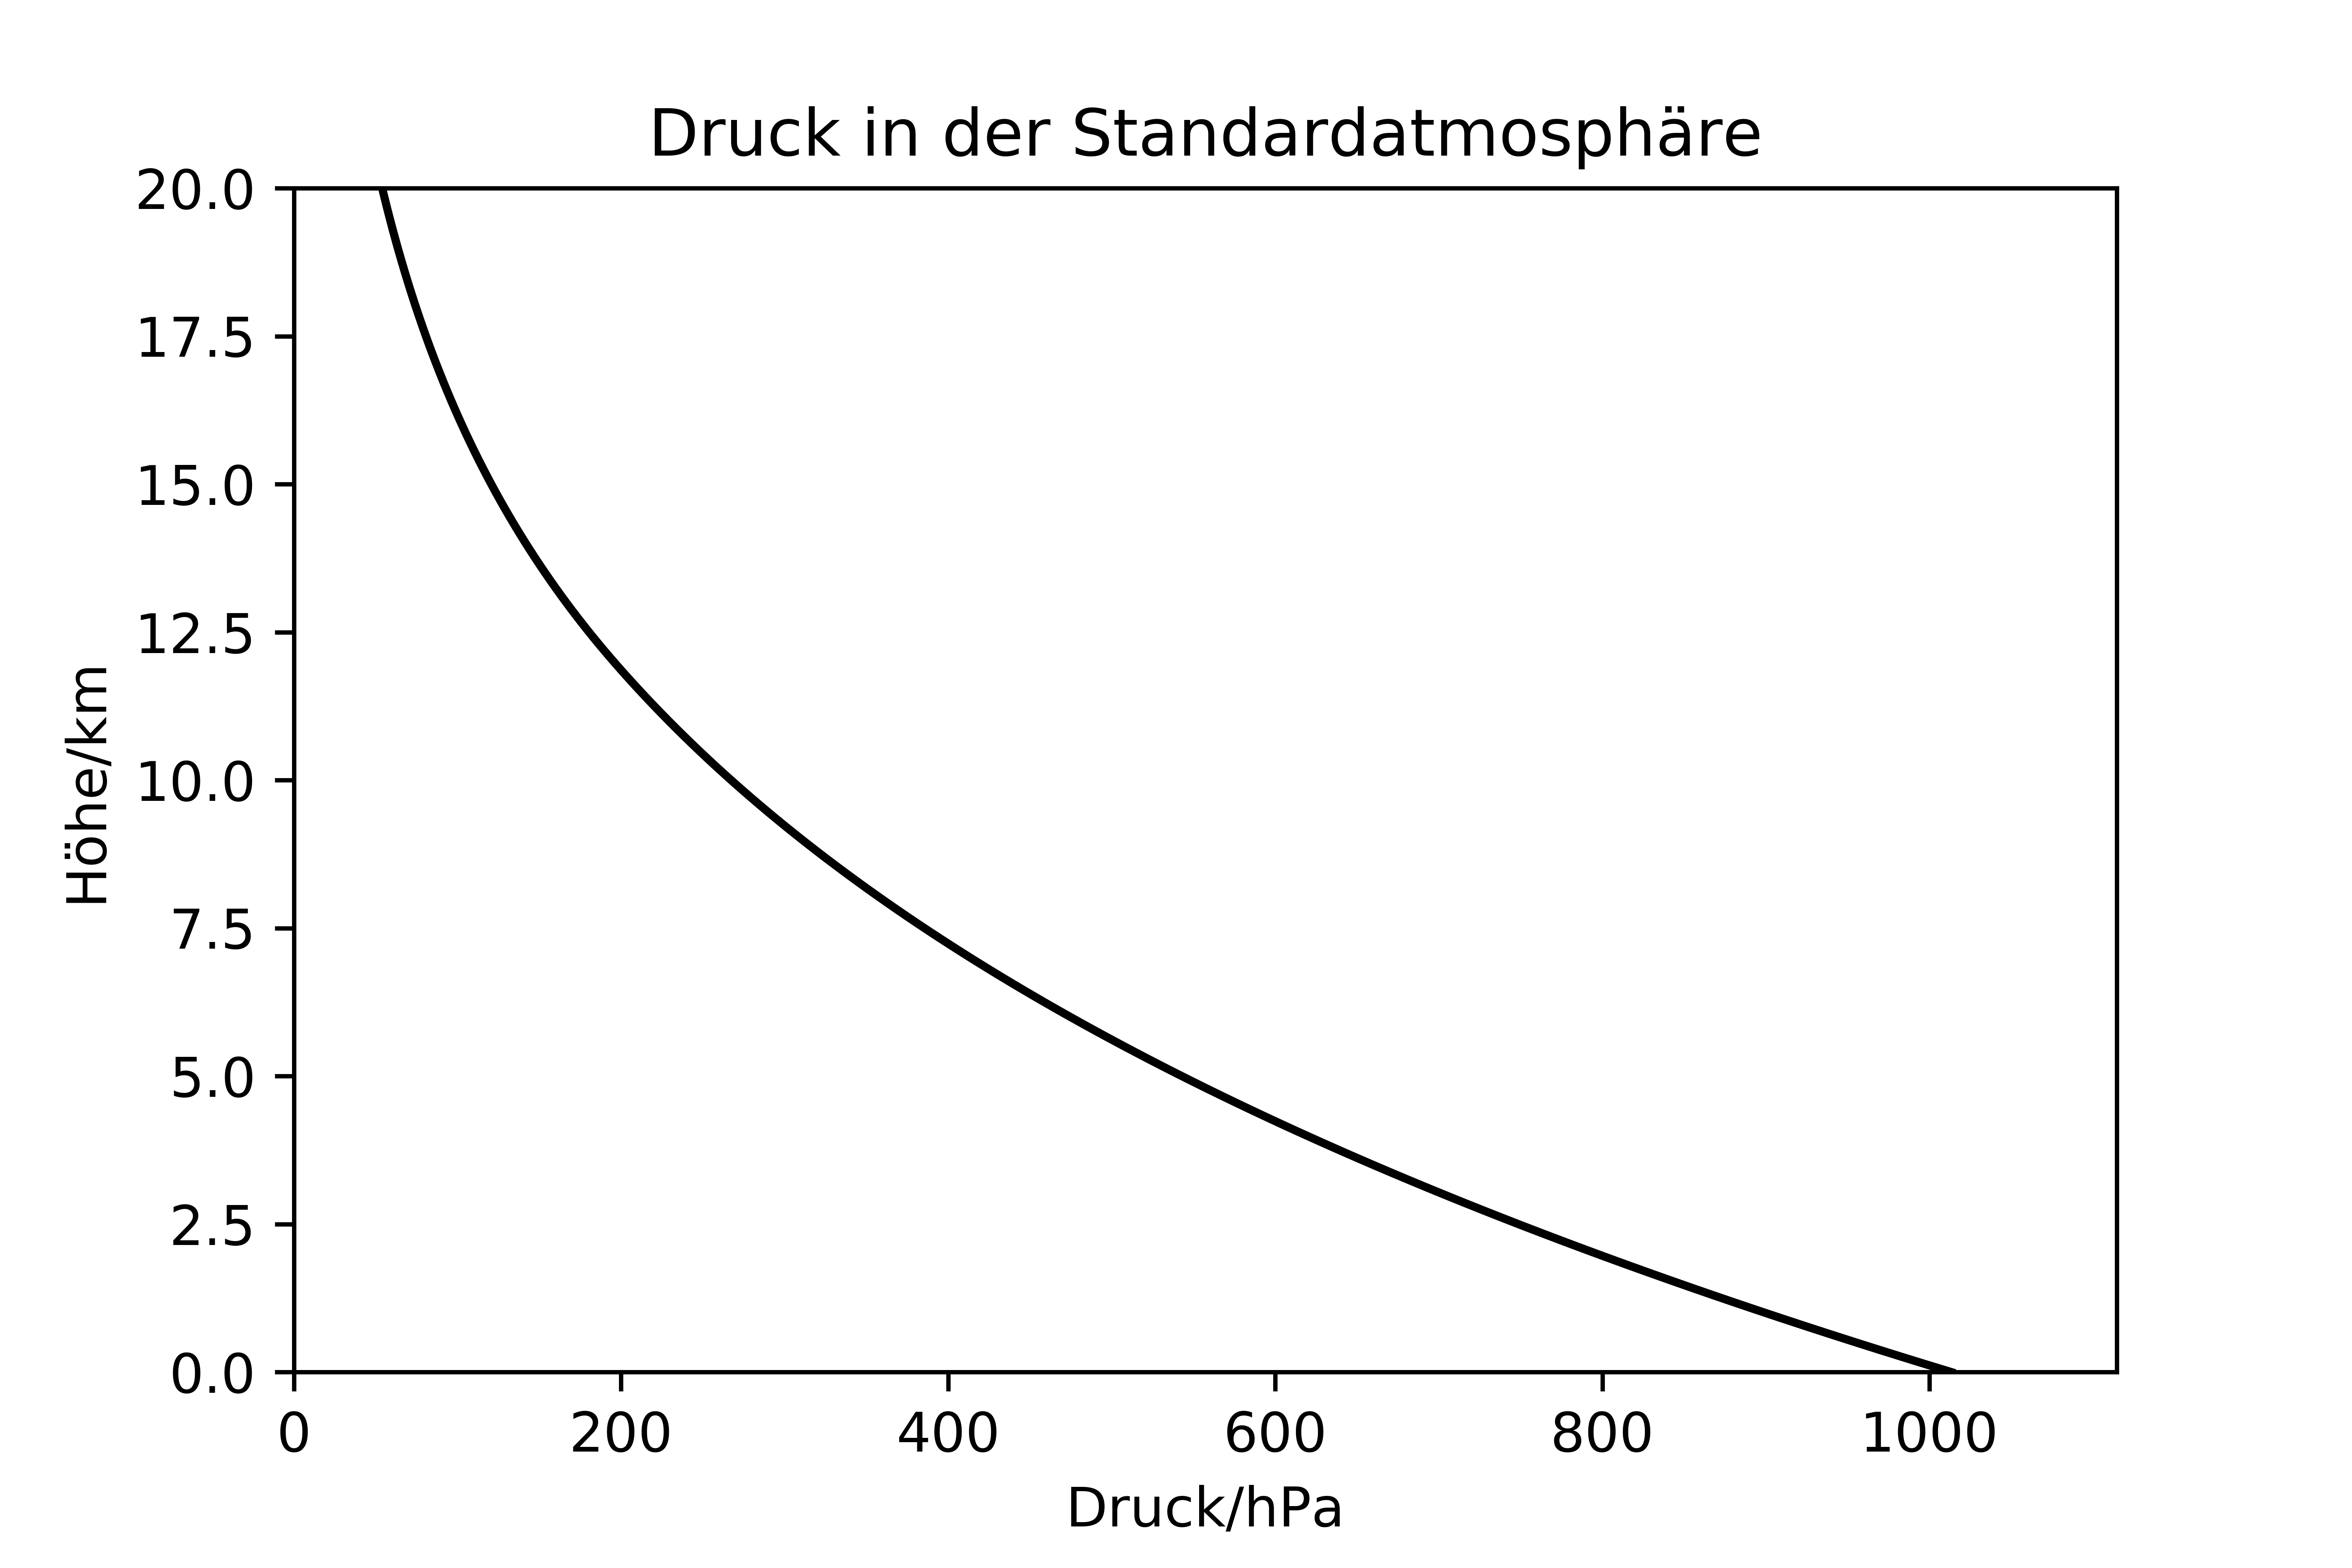
\includegraphics[height = 5cm]{figs/standard_atmosphere_pressure.png}
\end{subfigure}
\begin{subfigure}[c]{.49\textwidth}
\centering
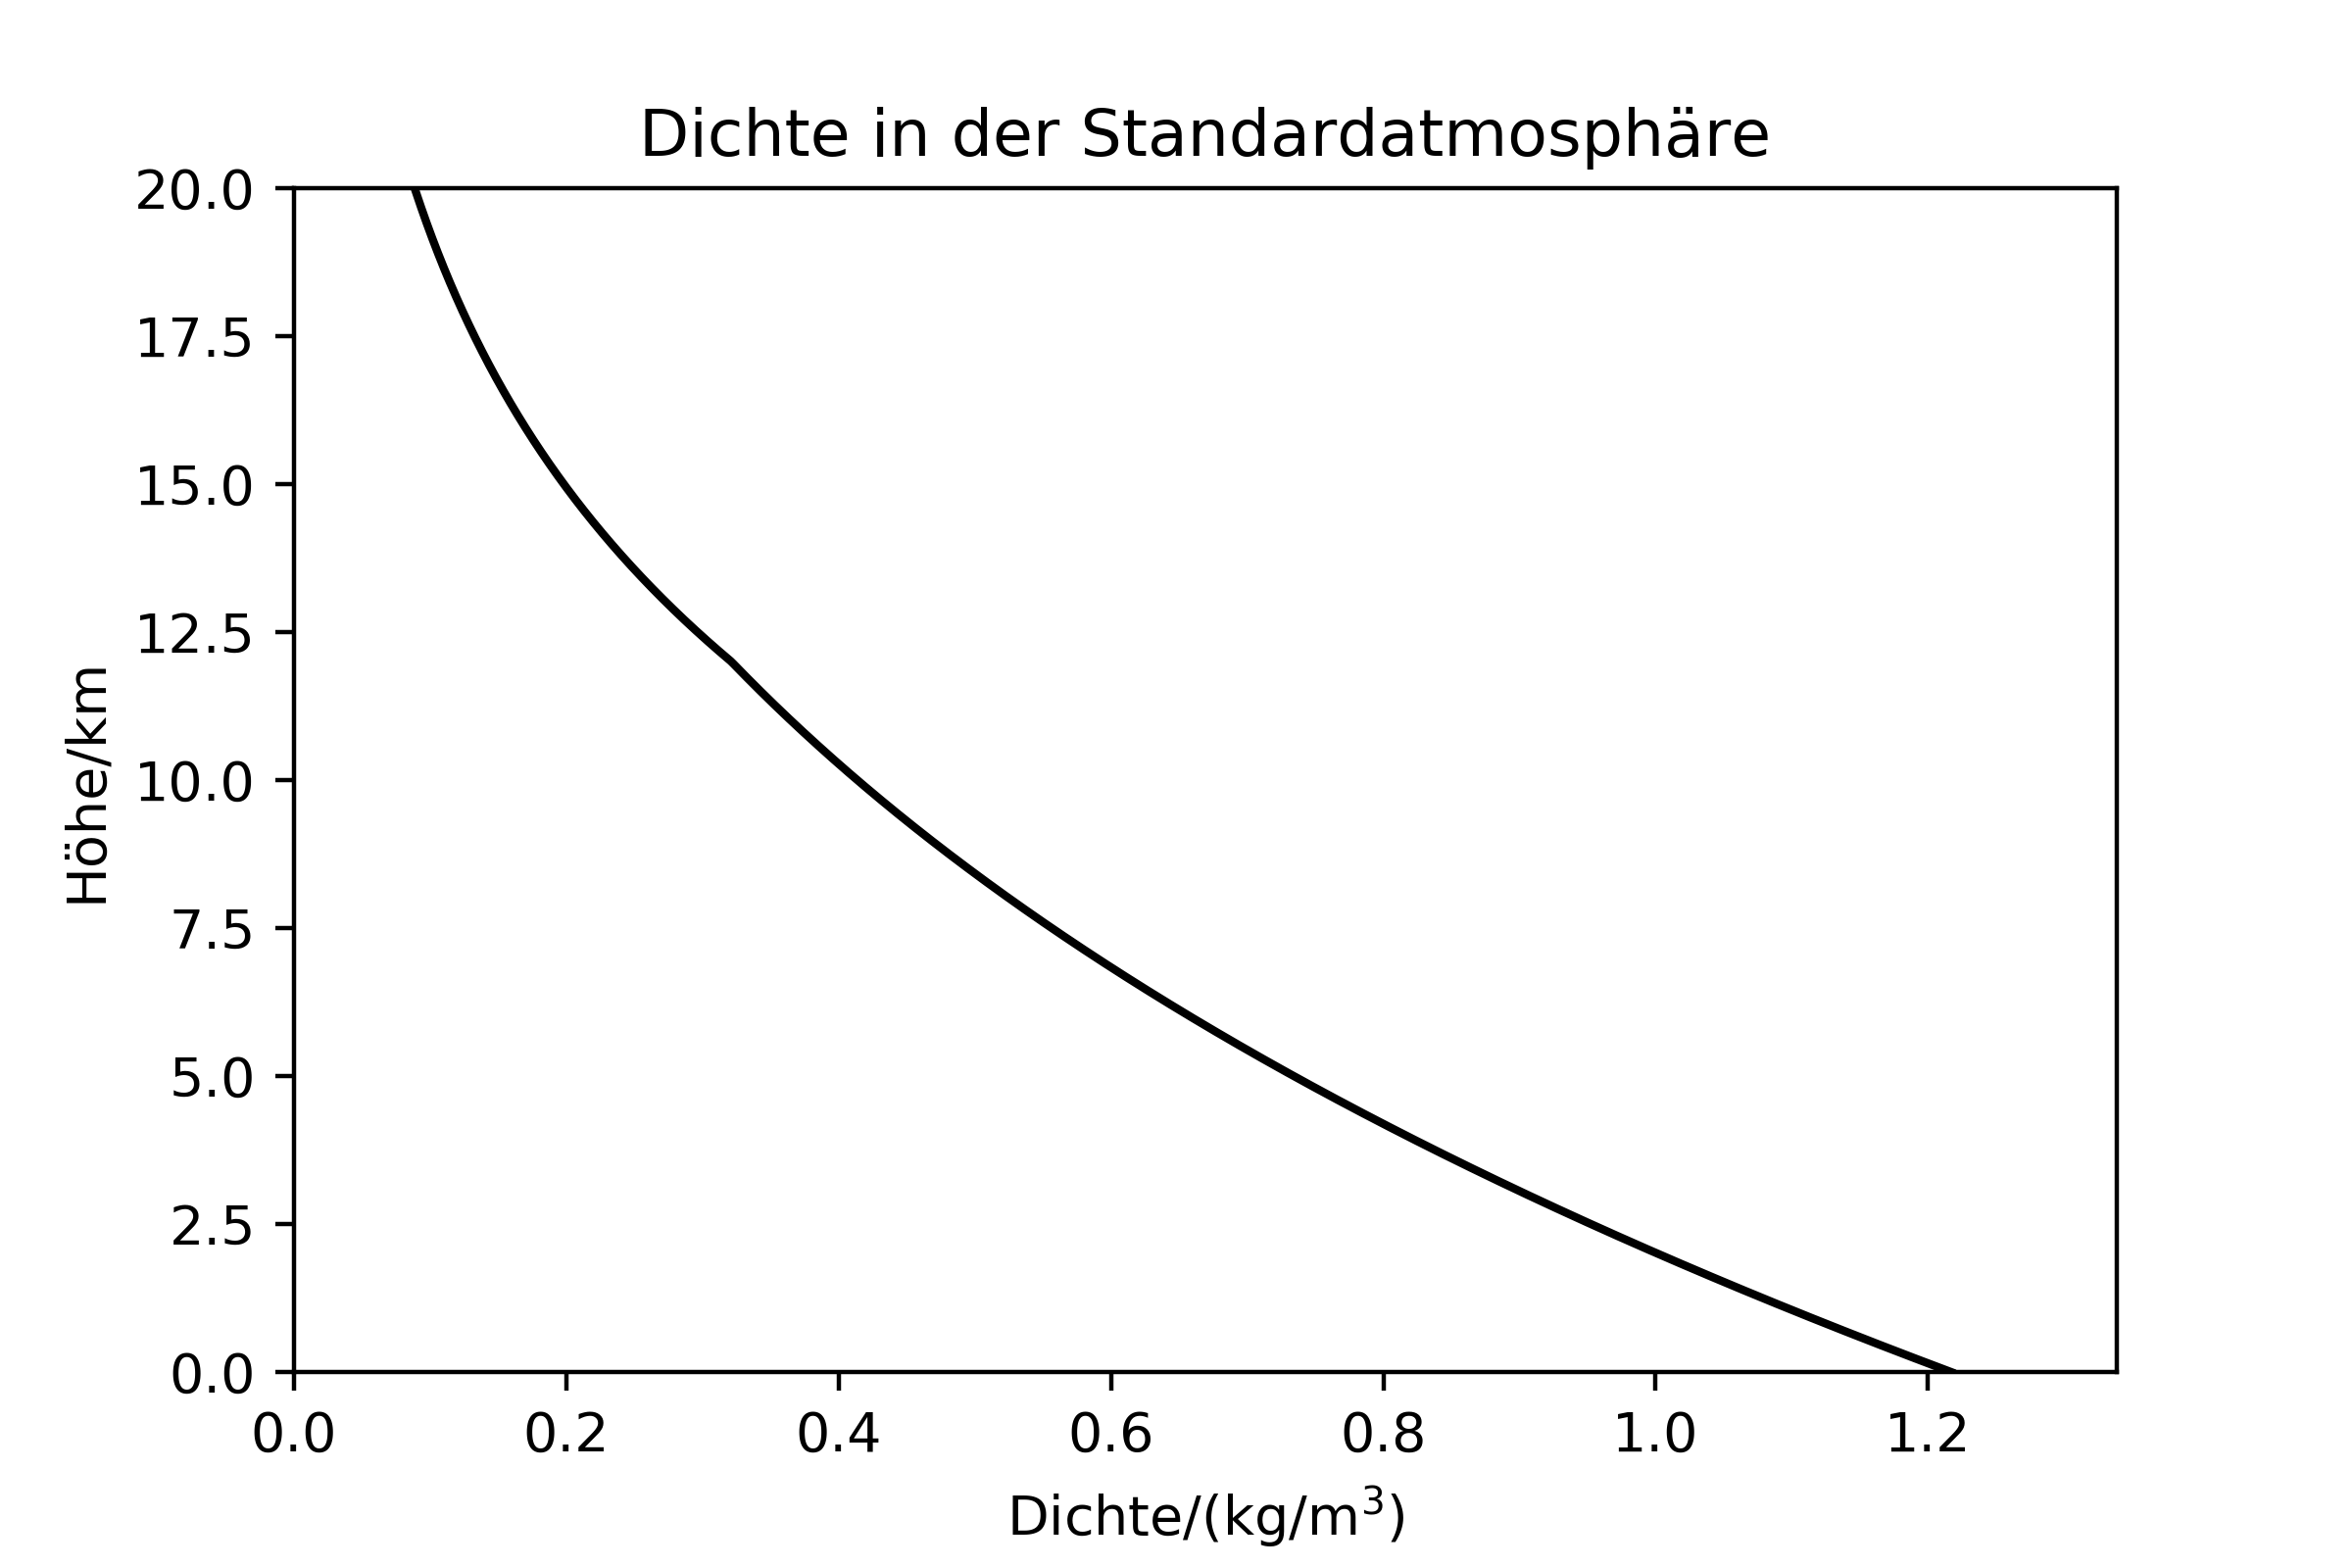
\includegraphics[height = 5cm]{figs/standard_atmosphere_density.png}
\end{subfigure}
\end{figure}

In einer stabilen Atmosphäre ist $\theta$ eine mögliche Vertikalkoordinate, man spricht von \index{isentrope Koordinate}\index{Koordinate!isentrope}\textit{isentropen Koordinaten}, da die Flächen gleicher Vertikalkoordinate Flächen gleicher Entropie sind.

\section{Kondensate}
\label{sec:tracer}\index{Kondensat}

Es muss der Erste Hauptsatz auch noch für die Kondensatklassen $i$ formuliert werden. Hierzu geht man von Glg. \eqref{eq:td1_without_mass} aus:
%
\begin{align}
\Delta U_i = \Delta Q_i - \Delta W_i
\end{align}
%
Bei den Kondensaten nimmt man Inkompressibilität an, also $\Delta W_i = 0$. Als Wärmequellen spielen neben Strahlung, Wärmeübergang, und Dissipation auch Phasenübergänge eine Rolle. Diese wirken auf zwei Arten:
%
\begin{itemize}
\item Sie führen zu latenten Wärmeflüssen und ändern so die Temperatur.
\item Sie ändern die Zusammensetzung der Bestandteile der Luft und ändern die Temperatur über Durchmischung.
\end{itemize}
%
Der erste Punkt wird in Kap. \ref{chap:konkretisierung_der_waermeflüsse} näher beschrieben. Alle Wärmeflüsse, die pro Volumen auf die Phase $i$ wirken, werden zu einer Quellstärke $q_i$ zusammengefasst. Hier soll es um den zweiten Punkt gehen, das heißt es soll die Einwirkung von Massenflüssen auf die Temperatur $T_i$ untersucht werden. Glg. \eqref{eq:quelle_kondensat_masse} umfasst fünf Arten von Massenflüssen, nämlich
%
\begin{itemize}
\item Phasenübergänge, bei denen neue Kondensatteilchen entstehen,
\item Phasenübergänge, die an der Oberfläche eines Partikels stattfinden,
\item Phasenumwandlungen von Kondensatteilchen, sodass diese ihre Klasse wechseln,
\item Kollisionen und
\item Zerfallsprozesse 
\end{itemize}
%
Es tragen nur solche Prozesse zu einer Änderung der Temperatur $T_i$ bei, bei denen Materie in die Phase $i$ übergeht. Die Klasse $i$ habe die spezifische Wärmekapazität $c_i$, die $m_j$ und $m_h$ seien die in die Phase $i$ übergehenden Massen. Dann gilt für den Wärmegehalt vor bzw. nach einem Massenfluss
%
\begin{align}
c_im_iT_i\left(t\right) + c_hm_hT + \sum_{j\not = i}^{}c_jm_jT_j & = c_iT_i\left(t + \Delta t\right)\left(m_h + m_i + \sum_{j\not = i}^{}m_j\right)\nonumber\\
\Leftrightarrow c_im_i\left[T_i\left(t + \Delta t\right) - T_i\left(t\right)\right] & = c_hm_hT + \sum_{j\not = i}^{}c_jm_jT_j - c_iT_i\left(t + \Delta t\right)\left(m_h + \sum_{j\not = i}^{}m_j\right)\nonumber\\
\Leftrightarrow\Delta T_i & = \frac{c_h}{c_im_i}m_h\left(T - \frac{c_i}{c_h}T_i\left(t + \Delta t\right)\right) + \frac{1}{c_im_i}\sum_{j\not = i}\left[c_jm_jT_j - c_im_jT_i\left(t + \Delta t\right)\right]\nonumber\\
\Leftrightarrow \frac{1}{\Delta V}\frac{dT_i}{dt} & = \frac{1}{m_i}\newtilde{q}_{hi}\left(\frac{c_h}{c_i}T - T_i\right) + \frac{1}{m_i}\sum_{j\not = i}^{}\newtilde{q}_{j, i}\left(\frac{c_j}{c_i}T_j - T_i\right)\nonumber\\
\Leftrightarrow\rho_ic_i\frac{dT_i}{dt} & = \newtilde{q}_{hi}\left(c_hT - c_iT_i\right) + \sum_{j}^{}\newtilde{q}_{j, i}\left(c_jT_j - c_iT_i\right).
\end{align}
%
Hierbei wurde davon ausgegangen, dass alle Teilchen der Klasse $i$ dieselbe Temperatur $T_i$ haben, dass also instantane Durchmischung eintritt. Nach Glg. \eqref{eq:quelle_kondensat_masse} und den Überlegungen in Absch. \ref{sec:phasenuebergangswaerme} gilt
%
\begin{align}
\newtilde{q}_{hi} = \newtilde{q}_{v, i}' + \newtilde{q}_{v, i}''.
\end{align}
%
Zu den $\newtilde{q}_{j, i}$ tragen Phasenumwandlungen, Kollisionen und Zerfallsprozesse bei. Nach den Überlegungen in der Herleitung von Glg. \eqref{eq:quelle_kondensat_masse} gilt
%
\begin{align}
\newtilde{q}_{j, i} = \newtilde{m}_j\sum_{k}^{}\sigma_{j, k}n_jn_k\newoverline{v_{\text{rel}}}\left(j, k\right)P_{j, k}\delta_{i, R_{j, k}} + \newtilde{m}_i\lambda_jn_j\sum_l\left(Z_{jil}\right) + \newtilde{q}_{j, i}'''.
\end{align}
%
Man hat also
%
\begin{center}
\doublebox{\parbox{0.97\textwidth}{
\begin{center}
\begin{align}
\rho_ic_i\frac{dT_i}{dt} & = q_i + \left(\newtilde{q}_{v, i}' + \newtilde{q}_{v, i}''\right)\left(c_hT - c_iT_i\right)\nonumber\\
& + \sum_{j}^{}\left[\newtilde{m}_j\sum_{k}^{}\sigma_{j, k}n_jn_k\newoverline{v_{\text{rel}}}\left(j, k\right)P_{j, k}\delta_{i, R_{j, k}} + \newtilde{m}_i\lambda_jn_j\sum_l\left(Z_{jil}\right) + \newtilde{q}_{j, i}'''\right]\left(c_jT_j - c_iT_i\right)\label{eq:td1_kondensate}
\end{align}
\end{center}
}}
\end{center}
%
Dabei wurde in der Notation explizit berücksichtigt, dass die isochore spezifische Wärmekapazität gemeint ist. Ein analoger Term ist auch für die feuchte Luft zu berücksichtigen:
%
\begin{center}
\doublebox{\parbox{0.8\textwidth}{
\begin{center}
\begin{align}
\rho_hc_h^{(v)}\md{T} & = q_h + \sum_i\left(\newtilde{q}_{v, i}' + \newtilde{q}_{v, i}''\right)\left(c_h^{(v)}T - c_iT_i\right)
\end{align}
\end{center}
}}
\end{center}

\chapter{\normalfont\textsc{Anwendung des Hamilton-Formalismus auf die Atmosphäre}}
\label{chap:anwendung_des_hamilton-formalismus_auf_die_atmosphaere}\index{Hamilton-Formalismus!Atmosphäre}\index{Atmosphäre!Hamilton-Formalismus}

Es ist sinnvoll, die Massendichte $\rho$ als erste prognostische Variable festzulegen und die Kontinuitätsgleichung
%
\begin{align}
\frac{\partial\rho}{\partial t} + \nabla\cdot\left(\rho\mathbf{v}\right) = 0
\end{align}
%
als erste prognostische Gleichung. Dies ist so, da die Masendichte eine sehr fundamentale Größe ist (sie beschreibt einfach, wie viel Masse sich an einem gewissen Ort befindet) und die Kontinuitätsgleichung in der Herleitung vieler anderer prognostischer Gleichungen enthalten ist. Aufgrund der thermischen Zustandsgleichung idealer Gase muss man genau eine weitere thermodynamische Variable $q_1 \not= \rho$ wählen, um den thermodynamischen Zustand des idealen Gases eindeutig festzulegen. Für die Hamilton-Funktion der Atmosphäre notiert man dann 
%
\begin{align}
H = H\left(\rho, q_1, \mathbf{v}\right) = \int_A\frac{1}{2}\rho\mathbf{v}^2 + \rho\phi + \newtilde{I}\left(\rho, q_1\right)d^3r.
\end{align}
%
$\newtilde{I}\left(\rho, q_1\right)$ ist die innere Energiedichte als Funktion der Massendichte und der prognostischen Variable $q_1$. In diesem funktionalen Zusammenhang ist die thermische Zustandsgleichung idealer Gase implizit enthalten.

Als Skalarprodukt\index{Skalarprodukt} zweier Funktionen skalarer Funktionen $f$, $g$ definiert man
%
\begin{align}
\left\langle f \big| g\right\rangle \coloneqq \int_Af^\star\left(\mathbf{r}, t\right)g\left(\mathbf{r}, t\right)d^3r.
\end{align}
%
Dies entspricht dem in der Quantenmechanik definierten unitären Produkt Glg. \eqref{eq:def_unitary_product}. Dabei lässt man für $f$ und $g$ reell- und komplexwertige Funktionen zu. Im Falle reeller Funktionen spielt die komplexe Konjugation von $f$ keine Rolle. Für vektorwertige Funktionen definiert man analog
%
\begin{align}
\left\langle\mathbf{f}\big|\mathbf{g}\right\rangle \coloneqq \int_A\mathbf{f}^\star\left(\mathbf{r}, t\right)\cdot\mathbf{g}\left(\mathbf{r}, t\right)d^3r.
\end{align}

\section{Reversible trockene Atmosphäre}
\label{sec:reversible_trockene_atmosphaere}

Sei $F$ ein beliebiges Funktional der atmosphärischen Zustandsvariablen. Die Zeitentwicklung von $F$ lässt sich laut Glg. \eqref{eq:poisson_bracket_prop_1} mittels der Poisson-Klammer als
%
\begin{align}
\frac{dF}{dt} = \left\lbrace F, H\right\rbrace + \frac{\partial F}{\partial t}.
\end{align}
%
notieren. Hängt $F$ nicht explizit von der Zeit ab, was im Regelfall so ist, folgt
%
\begin{center}
\doublebox{\parbox{0.8\textwidth}{
\begin{center}
\begin{align}
\frac{dF}{dt} = \left\lbrace F, H\right\rbrace.\label{eq:poisson_bracket_non_explicit_t}
\end{align}
\end{center}
}}
\end{center}
%
Um für $\left\lbrace F, H\right\rbrace$ einen expliziten Ausdruck herzuleiten, beginnt man, indem man in Glg. \eqref{eq:poisson_bracket_def} $K = H$ einsetzt:
%
\begin{align}
\left\lbrace F, H\right\rbrace \coloneqq \sum_{i = 1}^f\left(\frac{\partial F}{\partial q_i}\frac{\partial H}{\partial p_i} - \frac{\partial F}{\partial p_i}\frac{\partial H}{\partial q_i}\right)
\end{align}
%
Für die generalisierten Koordinaten werden nun die atmosphärischen Zustandsgrößen $\mathbf{u} = \left(\rho, q_1, \mathbf{v}\right)^T$ eingesetzt. Da es sich bei $F$ und $H$ jedoch um Funktionale handelt und die generalisierten koordinaten Funktionen sind, muss die Poisson-Klammer uunächst für diesen Fall verallgemeinert werden. Sei $f = f\left(\mathbf{u}\right)$ eine skalar- oder vektorwertige Funktion der atmosphärischen Zustandsfunktionen. Man kann nun ein zu $f$ gehöriges Funktional
%
\begin{align}
F\left[\mathbf{u}\right] &\coloneqq \int_Af\left(\mathbf{u}\right)d^3r
\end{align}
%
definieren. Leitet man dies nach der Zeit ab, erhält man
%
\begin{align}
\frac{dF\left[\mathbf{u}\right]}{dt} &= \int_A\frac{\partial f\left(\mathbf{u}\right)}{\partial t}d^3r = \int_A\frac{df\left(\mathbf{u}\right)}{d\mathbf{u}}\cdot\frac{\partial\mathbf{u}}{\partial t}d^3r,
\end{align}
%
wobei im letzten Schritt die mehrdimensionale Kettenregel genutzt wurde. Dies kann man weiter umformen zu
%
\begin{align}
\frac{dF\left[\mathbf{u}\right]}{dt} &= \left\lbrace F, H\right\rbrace = \int_A\frac{df\left(\mathbf{u}\right)}{d\rho}\cdot\frac{\partial\rho}{\partial t}d^3r + \int_A\frac{df\left(\mathbf{u}\right)}{dq_1}\cdot\frac{\partial q_1}{\partial t}d^3r + \int_A\frac{df\left(\mathbf{u}\right)}{d\mathbf{v}}\cdot\frac{\partial\mathbf{v}}{\partial t}d^3r.
\end{align}
%
Die Ableitungen von $f$ sind die sogenannten \textit{Funktionalableitungen}\index{Funktionalableitung} von $F$, man definiert
%
\begin{align}
\frac{\delta F}{\delta x} \coloneqq \frac{df}{dx}
\end{align}
%
für $x \in \left\{\rho, q_1, \mathbf{v}\right\}$. Somit gilt
%
\begin{align}
\frac{dF\left[\mathbf{u}\right]}{dt} &= \left\lbrace F, H\right\rbrace = \int_A\frac{\delta F}{\delta \rho}\frac{\partial\rho}{\partial t}d^3r + \int_A\frac{\delta F}{\delta q_1}\frac{\partial q_1}{\partial t}d^3r + \int_A\frac{\delta F}{\delta \mathbf{v}}\cdot\frac{\partial\mathbf{v}}{\partial t}d^3r.\label{eq:poisson_bracket_atm_gen_deriv_0}
\end{align}
%
Bei der Wahl von $q_1$ schränkt man sich nun Größen ein, für die
%
\begin{align}
\frac{\partial q_1}{\partial t} = -\nabla\cdot\left(q_1\mathbf{v}\right)\label{eq:deriv_q_1_entropy}
\end{align}
%
gilt. Definieren $q_1' \coloneqq \frac{q_1}{\rho}$, dann folgt aus Glg. \eqref{eq:deriv_q_1_entropy}
%
\begin{align}
\frac{\partial\left(\rho q_1'\right)}{\partial t} &= -\nabla\cdot\left(\rho q_1'\mathbf{v}\right)\nonumber\\
\Leftrightarrow q_1'\frac{\partial\rho}{\partial t} + \rho\frac{\partial q_1'}{\partial t} &= -q_1'\nabla\cdot\left(\rho\mathbf{v}\right) - \rho\mathbf{v}\cdot\nabla q_1'\nonumber\\
\stackrel{\text{Kontinuitätsglg.}}{\Leftrightarrow} \rho\frac{\partial q_1'}{\partial t} &= -\rho\mathbf{v}\cdot\nabla q_1' \Leftrightarrow \md{q_1'} = 0.
\end{align}
%
$q_1'$ ist also eine thermodynamische Zustandsgröße, welche sich bei adiabatischen Vorgängen nicht ändert. Dies impliziert
%
\begin{align}
q_1' = \frac{q_1}{\rho} = f\left(s\right),\label{eq:poisson_bracket_atm_gen_deriv_13}
\end{align}
%
wobei $s$ die spezifische Entropie ist.

Definiere $p_x$ für $x \in \left\{\rho, q_1, \mathbf{v}\right\}$ als zur Zustandsvariable $x$ gehörenden kanonischen Impuls. Aufgrund von Glg. \eqref{eq:hamilton_1} gilt
%
\begin{align}
\frac{\delta H}{\delta p_\rho} &= \frac{\partial\rho}{\partial t} = -\nabla\cdot\left(\rho\mathbf{v}\right),\label{eq:poisson_bracket_atm_gen_deriv_6}\\
\frac{\delta H}{\delta p_{q_1}} &= \frac{\partial q_1}{\partial t} = -\nabla\cdot\left(q_1\mathbf{v}\right) = -\nabla\cdot\left(\frac{q_1}{\rho}\rho\mathbf{v}\right),\label{eq:poisson_bracket_atm_gen_deriv_7}\\
\frac{\delta H}{\delta p_\mathbf{v}} &= \frac{\partial\mathbf{v}}{\partial t} =  -\frac{1}{\rho}\nabla p - \frac{\etabi}{\rho}\times\rho\mathbf{v} - \nabla\phi - \nabla k,\label{eq:poisson_bracket_atm_gen_deriv_8}
\end{align}
%
hierbei sind $\phi$ das Geopotential und $k$ die spezifische kinetische Energie. Für die global integrierte kinetische Energie $K$ der Atmosphäre gilt
%
\begin{align}
K \coloneqq \int_A\frac{1}{2}\rho\mathbf{v}^2d^3r.
\end{align}
%
Die Summe aus global integrierter innerer und potentieller Energie $I'$ lautet
%
\begin{align}
I' \coloneqq \int_A\newtilde{I} + \rho\phi d^3r = \int_A\rho\phi + c_d^{(v)}\rho Td^3r
\end{align}
%
Damit gilt $H = K + I'$, da $H$ die Gesamtenergie der Atmosphäre ist ($H$ ist nicht explizit zeitabhängig). Es gilt unabhängig von der Wahl von $q_1$
%
\begin{align}
\frac{\delta I'}{\delta\mathbf{v}} = 0 \Rightarrow \frac{\delta H}{\delta\mathbf{v}} = \frac{\delta K}{\delta\mathbf{v}} = \rho\mathbf{v}.\label{eq:poisson_bracket_atm_gen_deriv_9}
\end{align}
%
Für $K$ gilt weiterhin
%
\begin{align}
\frac{\delta K}{\delta q_1} &= 0,\label{eq:poisson_bracket_atm_gen_deriv_15}\\
\frac{\delta K}{\delta\rho} &= \frac{1}{2}\mathbf{v}^2 = k.
\end{align}
%
Setzt man dies in die Glg.en \eqref{eq:poisson_bracket_atm_gen_deriv_6} - \eqref{eq:poisson_bracket_atm_gen_deriv_8} ein, erhält man
%
\begin{align}
\frac{\delta H}{\delta p_\rho} &= \frac{\partial\rho}{\partial t} = -\nabla\cdot\frac{\delta H}{\delta\mathbf{v}},\label{eq:poisson_bracket_atm_gen_deriv_10}\\
\frac{\delta H}{\delta p_{q_1}} &= \frac{\partial q_1}{\partial t} = -\nabla\cdot\left(q_1\mathbf{v}\right) = -\nabla\cdot\left(\frac{q_1}{\rho}\frac{\delta H}{\delta\mathbf{v}}\right),\label{eq:poisson_bracket_atm_gen_deriv_11}\\
\frac{\delta H}{\delta p_\mathbf{v}} &= \frac{\partial\mathbf{v}}{\partial t} =  -\frac{1}{\rho}\nabla p - \frac{\etabi}{\rho}\times\frac{\delta H}{\delta\mathbf{v}} - \nabla\phi - \nabla\frac{\delta K}{\delta\rho},\label{eq:poisson_bracket_atm_gen_deriv_12}
\end{align}
%
Nun muss der Druckgradient in Termen von $H$ ausgedrückt werden. Nach Glg. \eqref{eq:chemisches_potential_prop_0} gilt
%
\begin{align}
p &= -\left(\frac{\partial E}{\partial V}\right)_{S, N},
\end{align}
%
wobei $E$ die Gesamtenergie des Systems ist. Als System verwendet man ein Luftteilchen, in einem solchen sind sowohl die Masse $m$ als auch die Teilchenzahl $N$ konstant. Die Gesamtenergie entspricht hier der inneren Energie $I$. Somit gilt
%
\begin{align}
p &= -\left(\frac{\partial I/m}{\partial V/m}\right)_{s} = -\left(\frac{\partial i}{\partial V/m}\right)_{s},
\end{align}
%
wobei $i = I/m$ die spezifische innere Energie ist. $\frac{V}{m} = \alpha = \frac{1}{\rho}$ ist das spezifische Volumen. Somit gilt
%
\begin{align}
p &= -\left(\frac{\partial i}{\partial\alpha}\right)_{s} = -\frac{\partial\rho}{\partial\alpha}\left(\frac{\partial i}{\partial\rho}\right)_{s} = \frac{1}{\alpha^2}\left(\frac{\partial i}{\partial\rho}\right)_{s} = \rho^2\left(\frac{\partial i}{\partial\rho}\right)_{s}.
\end{align}
%
Es gilt nun
%
\begin{align}
\left(\frac{\partial i}{\partial\rho}\right)_{s} &= \left(\frac{\partial i}{\partial\rho}\right)_{\newtilde{s}} + \left(\frac{\partial i}{\partial\newtilde{s}}\right)_{\rho}\frac{\partial\newtilde{s}}{\partial\rho}.
\end{align}
%
Für die innere Energiedichte $\newtilde{I}$ gilt
%
\begin{align}
\newtilde{I} = \rho i \Rightarrow i = \frac{\newtilde{I}}{\rho},
\end{align}
%
hieraus folgt
%
\begin{align}
p &= \rho^2\left(\frac{\partial\newtilde{I}/\rho}{\partial\rho}\right)_{\newtilde{s}} + \rho^2\left(\frac{\partial\newtilde{I}/\rho}{\partial\newtilde{s}}\right)_{\rho}\frac{\partial\newtilde{s}}{\partial\rho} = \rho\left(\frac{\partial\newtilde{I}}{\partial\rho}\right)_{\newtilde{s}} - \newtilde{I} + \newtilde{s}\left(\frac{\partial\newtilde{I}}{\partial\newtilde{s}}\right)_{\rho}.
\end{align}
%
Somit erhält man für den Druckgradienten
%
\begin{align}
\nabla p &= \left(\frac{\partial\newtilde{I}}{\partial\rho}\right)_{\newtilde{s}}\nabla\rho + \rho\nabla\left(\frac{\partial\newtilde{I}}{\partial\rho}\right)_{\newtilde{s}} - \nabla\newtilde{I} + \left(\frac{\partial\newtilde{I}}{\partial\newtilde{s}}\right)_{\rho}\nabla\newtilde{s} + \newtilde{s}\nabla\left(\frac{\partial\newtilde{I}}{\partial\newtilde{s}}\right)_{\rho}\nonumber\\
&= \left(\left(\frac{\partial\newtilde{I}}{\partial\rho}\right)_{\newtilde{s}}\nabla\rho + \left(\frac{\partial\newtilde{I}}{\partial\newtilde{s}}\right)_{\rho}\nabla\newtilde{s} - \nabla\newtilde{I}\right) + \rho\nabla\left(\frac{\partial\newtilde{I}}{\partial\rho}\right)_{\newtilde{s}}\newtilde{s}\nabla\left(\frac{\partial\newtilde{I}}{\partial\newtilde{s}}\right)_{\rho}\nonumber\\
&= \rho\nabla\left(\frac{\partial\newtilde{I}}{\partial\rho}\right)_{\newtilde{s}} + \newtilde{s}\nabla\left(\frac{\partial\newtilde{I}}{\partial\newtilde{s}}\right)_{\rho}.
\end{align}
%
Für die Druckgradientbeschleunigung gilt somit
%
\begin{align}
-\frac{1}{\rho}\nabla p &= -\nabla\left(\frac{\partial\newtilde{I}}{\partial\rho}\right)_{\newtilde{s}} - s\nabla\left(\frac{\partial\newtilde{I}}{\partial\newtilde{s}}\right)_{\rho}.\label{eq:poisson_bracket_atm_gen_deriv_14}
\end{align}
%
Aufgrund von Glg. \eqref{eq:poisson_bracket_atm_gen_deriv_13} ist $\frac{q_1}{\rho} = f\left(s\right)$, was
%
\begin{align}
\left(\frac{\partial i}{\partial x}\right)_s = \left(\frac{\partial i}{\partial x}\right)_{q_1/\rho}
\end{align}
%
impliziert. Somit kann Glg. \eqref{eq:poisson_bracket_atm_gen_deriv_14} zu
%
\begin{align}
-\frac{1}{\rho}\nabla p &= -\nabla\left(\frac{\partial\newtilde{I}}{\partial\rho}\right)_{q_1} - \frac{q_1}{\rho}\nabla\left(\frac{\partial\newtilde{I}}{\partial q_1}\right)_{\rho}.
\end{align}
%
verallgeminert werden. Dies kann man durch Funktionalableitungen der global integrierten inneren Energie $I$ ausdrücken:
%
\begin{align}
-\frac{1}{\rho}\nabla p &= -\nabla\left(\frac{\delta I}{\delta\rho}\right)_{q_1} - \frac{q_1}{\rho}\nabla\left(\frac{\delta I}{\delta q_1}\right)_{\rho}.
\end{align}
%
Mit Glg. \eqref{eq:poisson_bracket_atm_gen_deriv_15} folgt
%
\begin{align}
-\frac{1}{\rho}\nabla p &= -\nabla\left(\frac{\delta I}{\delta\rho}\right)_{q_1} - \frac{q_1}{\rho}\nabla\left(\frac{\delta H}{\delta q_1}\right)_{\rho}.
\end{align}
%
Setzt man dies in Glg. \eqref{eq:poisson_bracket_atm_gen_deriv_12} ein, erhält man
%
\begin{align}
\frac{\delta H}{\delta p_\mathbf{v}} &= \frac{\partial\mathbf{v}}{\partial t} = -\nabla\left(\frac{\delta I}{\delta\rho}\right)_{q_1} - \frac{q_1}{\rho}\nabla\left(\frac{\delta H}{\delta q_1}\right)_{\rho} - \frac{\etabi}{\rho}\times\frac{\delta H}{\delta\mathbf{v}} - \nabla\phi - \nabla\frac{\delta K}{\delta\rho}\nonumber\\
&= -\nabla\frac{\delta H}{\delta\rho} - \frac{q_1}{\rho}\nabla\frac{\delta H}{\delta q_1} - \frac{\etabi}{\rho}\times\frac{\delta H}{\delta\mathbf{v}}.\label{eq:poisson_bracket_atm_gen_deriv_16}
\end{align}
%
In der zweiten Zeile wurden dabei die Markierungen der konstant gehaltenen Größen weggelassen, da aus der Definition von $H$ eindeutig ist, wie die Ableitungen zu verstehen sind. Setzt man die Glg.en \eqref{eq:poisson_bracket_atm_gen_deriv_10} - \eqref{eq:poisson_bracket_atm_gen_deriv_11}, \eqref{eq:poisson_bracket_atm_gen_deriv_16} in Glg. \eqref{eq:poisson_bracket_atm_gen_deriv_0} ein, erhält man
%
\begin{align}
\left\lbrace F, H\right\rbrace &= -\int_A\frac{\delta F}{\delta\rho}\nabla\cdot\frac{\delta H}{\delta\mathbf{v}}d^3r - \int_A\frac{\delta F}{\delta q_1}\nabla\cdot\left(\frac{q_1}{\rho}\frac{\delta H}{\delta\mathbf{v}}\right)d^3r\nonumber\\
&-\int_A\frac{\delta F}{\delta\mathbf{v}}\cdot\left(\frac{\etabi}{\rho}\times\frac{\delta H}{\delta\mathbf{v}} + \nabla\frac{\delta H}{\delta\rho} + \frac{q_1}{\rho}\nabla\frac{\delta H}{\delta q_1}\right)d^3r.\label{eq:poisson_bracket_atm_gen_deriv_1}
\end{align}
%
Umsortierung ergibt
%
\begin{align}
\left\lbrace F, H\right\rbrace &= -\int_A\frac{\delta F}{\delta\rho}\nabla\cdot\frac{\delta H}{\delta\mathbf{v}} + \frac{\delta F}{\delta\mathbf{v}}\cdot\nabla\frac{\delta H}{\delta\rho}d^3r\nonumber\\
&- \int_A\frac{\delta F}{\delta q_1}\nabla\cdot\left(\frac{q_1}{\rho}\frac{\delta H}{\delta\mathbf{v}}\right) + \frac{\delta F}{\delta\mathbf{v}}\cdot\frac{q_1}{\rho}\nabla\frac{\delta H}{\delta q_1}d^3r\nonumber\\
&-\int_A\frac{\delta F}{\delta\mathbf{v}}\cdot\left(\frac{\etabi}{\rho}\times\frac{\delta H}{\delta\mathbf{v}}\right)d^3r.\label{eq:poisson_bracket_atm_gen_deriv_2}
\end{align}
%
Es gelten
%
\begin{align}
\frac{\delta F}{\delta\mathbf{v}}\cdot\nabla\frac{\delta H}{\delta\rho} &= \nabla\cdot\left(\frac{\delta H}{\delta\rho}\frac{\delta F}{\delta\mathbf{v}}\right) - \frac{\delta H}{\delta\rho}\nabla\cdot\left(\frac{\delta F}{\delta\mathbf{v}}\right),\\
\frac{\delta F}{\delta\mathbf{v}}\cdot\frac{q_1}{\rho}\nabla\frac{\delta H}{\delta q_1} &= \nabla\cdot\left(\frac{q_1}{\rho}\frac{\delta H}{\delta q_1}\frac{\delta F}{\delta\mathbf{v}}\right) - \frac{\delta H}{\delta q_1}\nabla\cdot\left(\frac{q_1}{\rho}\frac{\delta F}{\delta\mathbf{v}}\right).
\end{align}
%
Setzt man dies in Glg. \eqref{eq:poisson_bracket_atm_gen_deriv_2} ein, erhält man
%
\begin{align}
\left\lbrace F, H\right\rbrace &= -\int_A\frac{\delta F}{\delta\rho}\nabla\cdot\frac{\delta H}{\delta\mathbf{v}} + \nabla\cdot\left(\frac{\delta H}{\delta\rho}\frac{\delta F}{\delta\mathbf{v}}\right) - \frac{\delta H}{\delta\rho}\nabla\cdot\left(\frac{\delta F}{\delta\mathbf{v}}\right)d^3r\nonumber\\
&- \int_A\frac{\delta F}{\delta q_1}\nabla\cdot\left(\frac{q_1}{\rho}\frac{\delta H}{\delta\mathbf{v}}\right) + \nabla\cdot\left(\frac{q_1}{\rho}\frac{\delta H}{\delta q_1}\frac{\delta F}{\delta\mathbf{v}}\right) - \frac{\delta H}{\delta q_1}\nabla\cdot\left(\frac{q_1}{\rho}\frac{\delta F}{\delta\mathbf{v}}\right)d^3r\nonumber\\
&-\int_A\frac{\delta F}{\delta\mathbf{v}}\cdot\left(\frac{\etabi}{\rho}\times\frac{\delta H}{\delta\mathbf{v}}\right)d^3r.
\end{align}
%
Man geht nun von
%
\begin{align}
\int_A\nabla\cdot\left(\frac{\delta H}{\delta\rho}\frac{\delta F}{\delta\mathbf{v}}\right)d^3r = \int_A\nabla\cdot\left(\frac{q_1}{\rho}\frac{\delta H}{\delta q_1}\frac{\delta F}{\delta\mathbf{v}}\right)d^3r = 0
\end{align}
%
aus, was aufgrund des Satzes von Gauß erfüllt ist, falls $\frac{\delta F}{\delta\mathbf{v}}\cdot\mathbf{n} = 0$ auf $\partial A$ gilt. Unter diesen Voraussetzungen gilt also in einer reversiblen trockenen Atmosphäre für beliebige Funktionale $F$ die Zeitentwicklungsgleichung
%
\begin{center}
\doublebox{\parbox{0.95\textwidth}{
\begin{center}
\begin{align}
\frac{dF}{dt} = \lbrace F, H\rbrace &= -\int_A\frac{\delta F}{\delta\rho}\nabla\cdot\frac{\delta H}{\delta\mathbf{v}} - \frac{\delta H}{\delta\rho}\nabla\cdot\frac{\delta F}{\delta\mathbf{v}}d^3r\nonumber\\
&- \int_A\frac{\delta F}{\delta q_1}\nabla\cdot\left(\frac{q_1}{\rho}\frac{\delta H}{\delta\mathbf{v}}\right) - \frac{\delta H}{\delta q_1}\nabla\cdot\left(\frac{q_1}{\rho}\frac{\delta F}{\delta\mathbf{v}}\right)d^3r\nonumber\\
&- \int_A\frac{\delta F}{\delta\mathbf{v}}\cdot\left(\frac{\etabi}{\rho}\times\frac{\delta H}{\delta\mathbf{v}}\right)d^3r.\label{eq:poisson_bracket_atm_gen_explicit}
\end{align}
\end{center}
}}
\end{center}
%
Hieraus ergibt sich erwartungsgemäß
%
\begin{align}
\lbrace H, H\rbrace &= 0.
\end{align}
%
Man definiert nun
%
\begin{align}
\lbrace F, H\rbrace_\rho &\coloneqq -\int_A\frac{\delta F}{\delta\rho}\nabla\cdot\frac{\delta H}{\delta\mathbf{v}} - \frac{\delta H}{\delta\rho}\nabla\cdot\frac{\delta F}{\delta\mathbf{v}}d^3r = -\int_A-\frac{\delta H}{\delta\mathbf{v}}\cdot\nabla\frac{\delta F}{\delta\rho} + \frac{\delta F}{\delta\mathbf{v}}\cdot\nabla\frac{\delta H}{\delta\rho}d^3r\nonumber\\
&= -\int_A\frac{\delta F}{\delta\mathbf{v}}\cdot\nabla\frac{\delta H}{\delta\rho} - \frac{\delta H}{\delta\mathbf{v}}\cdot\nabla\frac{\delta F}{\delta\rho}d^3r,\\
\lbrace F, H\rbrace_{q_1} &\coloneqq -\int_A\frac{\delta F}{\delta q_1}\nabla\cdot\left(\frac{q_1}{\rho}\frac{\delta H}{\delta\mathbf{v}}\right) - \frac{\delta H}{\delta q_1}\nabla\cdot\left(\frac{q_1}{\rho}\frac{\delta F}{\delta\mathbf{v}}\right)d^3r = -\int_A-\frac{q_1}{\rho}\frac{\delta H}{\delta\mathbf{v}}\cdot\nabla\frac{\delta F}{\delta q_1} + \frac{q_1}{\rho}\frac{\delta F}{\delta\mathbf{v}}\cdot\nabla\frac{\delta H}{\delta q_1}d^3r\nonumber\\
&= -\int_A\frac{q_1}{\rho}\frac{\delta F}{\delta\mathbf{v}}\cdot\nabla\frac{\delta H}{\delta q_1} - \frac{q_1}{\rho}\frac{\delta H}{\delta\mathbf{v}}\cdot\nabla\frac{\delta F}{\delta q_1}d^3r
\end{align}
%
Es wird deutlich, dass jede Klammer in einer \glqq Skalarfeld x Divergenz\grqq- und in einer \glqq Vektorfeld x Gradient\grqq-Schreibweise formuliert werden kann. Jede der beiden Klammern ist antisymmetrisch:
%
\begin{align}
\lbrace F, H\rbrace_\rho &= -\lbrace H, F\rbrace_\rho\label{eq:poisson_bracket_atm_gen_deriv_3}\\
\lbrace F, H\rbrace_{q_1} &= -\lbrace H, F\rbrace_{q_1}\label{eq:poisson_bracket_atm_gen_deriv_4}
\end{align}
%
Nun definiert man sogenannte \textit{Nambu-Klammern}\index{Nambu-Klammer} durch
%
\begin{align}
\lbrace F, g, H\rbrace &\coloneqq -\int_A\frac{\delta F}{\delta\mathbf{v}}\cdot\left(\frac{1}{\rho}\frac{\delta g}{\delta\mathbf{v}}\times\frac{\delta H}{\delta\mathbf{v}}\right)d^3r = -\int_A\frac{1}{\rho}\frac{\delta F}{\delta\mathbf{v}}\cdot\left(\frac{\delta g}{\delta\mathbf{v}}\times\frac{\delta H}{\delta\mathbf{v}}\right)d^3r,
\end{align}
%
hierbei ist $g$ ein Funktional. Für Nambu-Klammern\index{Nambu-Klammer} gilt
%
\begin{align}
\lbrace F, g, H\rbrace = \lbrace H, F, g\rbrace = \lbrace g, H, F\rbrace.
\end{align}
%
Ferner gilt
%
\begin{align}
\lbrace F, g, H\rbrace = -\lbrace F, H, g\rbrace = -\lbrace g, F, H\rbrace = -\lbrace H, g, F\rbrace.\label{eq:poisson_bracket_atm_gen_deriv_5}
\end{align}
%
Setzt man dies zusammen mit den Glg.en \eqref{eq:poisson_bracket_atm_gen_deriv_3} - \eqref{eq:poisson_bracket_atm_gen_deriv_4} in Glg. \eqref{eq:poisson_bracket_atm_gen_parts} ein, erhält man

%
\begin{align}
\lbrace H, F\rbrace &= \lbrace H, F\rbrace_\rho + \lbrace H, F\rbrace_{q_1} + \lbrace H, h_a, F\rbrace = -\lbrace F, H\rbrace_\rho - \lbrace F, H\rbrace_{q_1} - \lbrace F, h_a, H\rbrace = -\lbrace F, H\rbrace.
\end{align}
%
Definiere nun eine \textit{reduzierte Helizität}\index{Helizität} $Z$ (für die originale Definition der Helizität siehe Glg. \eqref{eq:def_helicity}) durch
%
\begin{align}
Z \coloneqq \frac{1}{2}\mathbf{v}\cdot\nabla\times\mathbf{v}
\end{align}
%
und die {absolute Helizität}\index{absolute Helizität}\index{Helizität!absolute} $Z_a$ durch
%
\begin{align}
Z_a \coloneqq \frac{1}{2}\mathbf{v}_a\cdot\nabla\times\mathbf{v}_a = \frac{1}{2}\left(\Omegabi\times\mathbf{r} + \mathbf{v}\right)\cdot\nabla\times\left(\Omegabi\times\mathbf{r} + \mathbf{v}\right),
\end{align}
%
dies ist die im Inertialsystem gemessene Helizität\index{Helizität}. Die entsprechenden Funktionale werden durch
%
\begin{align}
Z &\coloneqq \int_A\frac{1}{2}\mathbf{v}\cdot\nabla\times\mathbf{v}d^3r,\\
Z_a &\coloneqq \int_A\frac{1}{2}\mathbf{v}_a\cdot\nabla\times\mathbf{v}_ad^3r
\end{align}
%
definiert. Seien nun $\mathbf{h}: A \to\mathbb{R}^3$ eine Testfunktion mit $\mathbf{h}\left(\partial A\right) = \mathbf{0}$ und $\epsilon > 0$. Man definiert
%
\begin{align}
Z'\left(\epsilon\right) &\coloneqq \int_A\frac{1}{2}\left(\mathbf{v} + \epsilon\mathbf{h}\right)\cdot\nabla\times\left(\mathbf{v} + \epsilon\mathbf{h}\right)d^3r = \int_A\frac{1}{2}\mathbf{v}\cdot\nabla\times\mathbf{v}d^3r + \int_A\frac{\epsilon}{2}\mathbf{h}\cdot\nabla\times\mathbf{v}d^3r + \int_A\frac{\epsilon}{2}\mathbf{v}\cdot\nabla\times\mathbf{h}d^3r + \mathcal{O}\left(\epsilon^2\right).
\end{align}
%
Es gilt nun in erster Ordnung in $\epsilon$ die Gleichung
%
\begin{align}
\frac{Z'\left(\epsilon\right) - Z'\left(0\right)}{\epsilon} &= \frac{Z'\left(\epsilon\right) - Z}{\epsilon} = \int_A\frac{1}{2}\mathbf{h}\cdot\nabla\times\mathbf{v}d^3r + \int_A\frac{1}{2}\mathbf{v}\cdot\nabla\times\mathbf{h}d^3r = \frac{1}{2}\int_A\mathbf{h}\cdot\nabla\times\mathbf{v} + \mathbf{v}\cdot\nabla\times\mathbf{h}d^3r\nonumber\\
&= \frac{1}{2}\int_A\mathbf{v}\cdot\nabla\times\mathbf{h} - \mathbf{h}\cdot\nabla\times\mathbf{v} + 2\mathbf{h}\cdot\nabla\times\mathbf{v}d^3r \stackrel{\text{Glg. \eqref{eq:diff_op_rule_9}}}{=} \frac{1}{2}\int_A\nabla\cdot\left(\mathbf{h}\times\mathbf{v}\right) + 2\mathbf{h}\cdot\nabla\times\mathbf{v}d^3r\nonumber\\
&= \int_A\mathbf{h}\cdot\nabla\times\mathbf{v}d^3r.
\end{align}
%
Im letzten Schritt wurden dabei der Gauß'sche Satz und die Tatsache $\mathbf{h}\left(\partial A\right) = \mathbf{0}$ eingesetzt. Somit gilt
%
\begin{align}
\frac{\delta Z}{\delta\mathbf{v}} = \nabla\times\mathbf{v} = \zetabi.
\end{align}
%
Analog gilt auch
%
\begin{align}
\frac{\delta Z_a}{\delta\mathbf{v}_a} = \nabla\times\mathbf{v}_a = \etabi.
\end{align}
%
Aufgrund von
%
\begin{align}
\frac{\delta Z}{\delta\mathbf{v}} = \frac{\delta H}{\delta\mathbf{v}_a}
\end{align}
%
gilt auch
%
\begin{align}
\frac{\delta Z_a}{\delta\mathbf{v}} = \etabi.
\end{align}
%
Somit kann man Glg. \eqref{eq:poisson_bracket_atm_gen_explicit} in der Form
%
\begin{center}
\doublebox{\parbox{0.95\textwidth}{
\begin{center}
\begin{align}
\frac{dF}{dt} = \lbrace F, H\rbrace &= \lbrace F, Z_a, H + \lbrace F, H\rbrace_\rho + \lbrace F, H\rbrace_{q_1}\rbrace\label{eq:poisson_bracket_atm_gen_parts}
\end{align}
\end{center}
}}
\end{center}
%
schreiben.

\subsection{Semi-prognostische Variable}
\label{sec:semi-prognostische_variable}\index{semi-prognostische Variable}\index{Variable!semi-prognostische}

Der Poisson-Klammer-Formalismus\index{Poisson-Klammer} führt auf eine spezielle Form der Druckgradientbeschleunigung. Darin ist neben $\rho$ und $q_1$ meist eine dritte Variable enthalten, gelegentlich sogar eine vierte oder fünfte. Eine dieser Variablen wählt man als sogenannte \textit{semi-prognostische Variable}\index{semi-prognostische Variable}\index{Variable!semi-prognostische} $q_2$. Diese ist aufgrund der thermischen Zustandsgleichung idealer Gase keine eigenständige prognostische Variable mehr, da der thermodynamische Zustand sonst überbestimmt wäre, jedoch ist sie gegenüber anderen diagnostischen Variablen ausgezeichnet, da sie in der Evolution der Energieformen eine Rolle spielt.

\subsubsection{Energieerhaltung aus Poisson-Klammer-Perspektive}
\label{sec:energieerhaltung_aus_poisson-klammer-perspektive}

Es gilt für Energieformen $F$ die Tatsache $\frac{\delta F}{\delta\mathbf{v}} \parallel \mathbf{v}$, somit gilt in diesem Fall
%
\begin{align}
\lbrace F, H_a, H\rbrace = 0 \Rightarrow \lbrace F, H\rbrace = \lbrace F, H\rbrace_\rho + \lbrace F, H\rbrace_{q_1}.
\end{align}
%
Hieraus folgen
%
\begin{align}
\lbrace K, H\rbrace &= \int_A-\frac{\delta K}{\delta\rho}\nabla\cdot\frac{\delta H}{\delta\mathbf{v}} + \frac{\delta H}{\delta\rho}\nabla\cdot\frac{\delta K}{\delta\mathbf{v}} + \frac{\delta H}{\delta q_1}\nabla\cdot\left(\frac{q_1}{\rho}\frac{\delta K}{\delta\mathbf{v}}\right)d^3r\nonumber\\
& = \int_A-\frac{\delta K}{\delta\rho}\nabla\cdot\frac{\delta H}{\delta\mathbf{v}} + \frac{\delta H}{\delta\rho}\nabla\cdot\frac{\delta H}{\delta\mathbf{v}} + \frac{\delta H}{\delta q_1}\nabla\cdot\left(\frac{q_1}{\rho}\frac{\delta H}{\delta\mathbf{v}}\right)d^3r\nonumber\\
& = \int_A\frac{\delta\left(H - K\right)}{\delta\rho}\nabla\cdot\frac{\delta H}{\delta\mathbf{v}} + \frac{\delta I'}{\delta q_1}\nabla\cdot\left(\frac{q_1}{\rho}\frac{\delta H}{\delta\mathbf{v}}\right)d^3r\nonumber\\
& = \int_A\frac{\delta I'}{\delta\rho}\nabla\cdot\frac{\delta H}{\delta\mathbf{v}} + \frac{\delta I'}{\delta q_1}\nabla\cdot\left(\frac{q_1}{\rho}\frac{\delta H}{\delta\mathbf{v}}\right)d^3r,\\
\lbrace I', H\rbrace & = \int_A-\frac{\delta I'}{\delta\rho}\nabla\cdot\frac{\delta H}{\delta\mathbf{v}} - \frac{\delta I'}{\delta q_1}\nabla\cdot\left(\frac{q_1}{\rho}\frac{\delta H}{\delta\mathbf{v}}\right)d^3r.
\end{align}
%
Addiert man beides, erhält man wie erwartet
%
\begin{align}
\lbrace K, H\rbrace + \lbrace I', H\rbrace = \lbrace H, H\rbrace = 0.
\end{align}

\subsection{Potentielle Temperatur als prognostische Variable}
\label{sec:potentielle_temperatur_als_prognostische_variable_hamilton}

Verwendet man anstatt der Temperatur die potentielle Temperatur und definiert
%
\begin{align}
q_1 \coloneqq \newtilde{\theta} = \rho\theta,
\end{align}
%
folgt mit Glg. \eqref{eq:state_theta}
%
\begin{align}
H & = H\left(\mathbf{v}, \rho, q_1\right) = H\left(\mathbf{v}, \rho, \newtilde{\theta}\right) = \int_A\frac{1}{2}\rho\mathbf{v}^2 + \rho\phi + c_d^{(v)}\frac{p\left(\rho, \newtilde{\theta}\right)}{R_d}d^3r\nonumber\\
& = \int_A\frac{1}{2}\rho\mathbf{v}^2 + \rho\phi + c_d^{(v)}\frac{p_0}{R_d}\left(\frac{R_d\newtilde{\theta}}{p_0}\right)^\kappa d^3r = \int_A\frac{1}{2}\rho\mathbf{v}^2 + \rho\phi + c_d^{(v)}\frac{p_0}{R_d}\left(\frac{R_d q_1}{p_0}\right)^\kappa d^3r.
\end{align}
%
Die Funktionalableitungen hiervon sind
%
\begin{align}
\frac{\delta H}{\delta\rho} & = \frac{1}{2}\mathbf{v}^2 + \phi,\\
\frac{\delta H}{\delta q_1} & = c_d^{(v)}\frac{p_0}{R_d}\frac{R_d}{p_0}\kappa\left(\frac{R_d q_1}{p_0}\right)^{\kappa - 1} = c_d^{(p)}\left(\frac{R_d q_1}{p_0}\right)^{\kappa - 1} = c_d^{(p)}\left(\frac{R_d q_1}{p_0}\right)^{\frac{R_d}{c_d^{(v)}}} \stackrel{\text{Glg. \eqref{eq:exner_pressure_diag}}}{=} c_d^{(p)}\Pi,\\
\frac{\delta H}{\delta\mathbf{v}} & = \rho\mathbf{v}.
\end{align}
%
Nun sollen die Zeitentwicklungen der Größen $K$ und $I'$ untersucht werden. Dazu rechnet man vorbereitend
%
\begin{align}
\frac{\delta K}{\delta\rho} = \frac{1}{2}\mathbf{v}^2, && \frac{\delta K}{\delta q_1} = 0, && \frac{\delta K}{\delta\mathbf{v}} = \rho\mathbf{v},\\
\frac{\delta I'}{\delta\rho} = \phi, && \frac{\delta I'}{\delta q_1} = c_d^{(p)}\Pi, \frac{\delta I'}{\delta\mathbf{v}} = 0.
\end{align}
%
und erhält somit
%
\begin{align}
\lbrace K, H\rbrace &= \int_A\frac{\delta H}{\delta\rho}\nabla\cdot\frac{\delta K}{\delta\mathbf{v}} - \frac{\delta K}{\delta\rho}\nabla\cdot\frac{\delta H}{\delta\mathbf{v}} + \frac{\delta H}{\delta q_1}\nabla\cdot\left(\frac{q_1}{\rho}\frac{\delta K}{\delta\mathbf{v}}\right) - \frac{\delta K}{\delta q_1}\nabla\cdot\left(\frac{q_1}{\rho}\frac{\delta H}{\delta\mathbf{v}}\right)d^3r\nonumber\\
&= \int_A\left(\frac{1}{2}\mathbf{v}^2 + \phi\right)\nabla\cdot\left(\rho\mathbf{v}\right) - \frac{1}{2}\mathbf{v}^2\nabla\cdot\left(\rho\mathbf{v}\right) + c_d^{(p)}\Pi\nabla\cdot\left(q_1\mathbf{v}\right)d^3r\nonumber\\
&= \int_A\phi\nabla\cdot\left(\rho\mathbf{v}\right) + c_d^{(p)}\Pi\nabla\cdot\left(q_1\mathbf{v}\right)d^3r\nonumber\\
&= \int_A-\rho\mathbf{v}\cdot\nabla\phi - c_d^{(p)}q_1\mathbf{v}\cdot\nabla\Pi d^3r,
\end{align}
\begin{align}
\lbrace I', H\rbrace &= \int_A\frac{\delta H}{\delta\rho}\nabla\cdot\frac{\delta I'}{\delta\mathbf{v}} - \frac{\delta I'}{\delta\rho}\nabla\cdot\frac{\delta H}{\delta\mathbf{v}} + \frac{\delta H}{\delta q_1}\nabla\cdot\left(\frac{q_1}{\rho}\frac{\delta I'}{\delta\mathbf{v}}\right) - \frac{\delta I'}{\delta q_1}\nabla\cdot\left(\frac{q_1}{\rho}\frac{\delta H}{\delta\mathbf{v}}\right)d^3r\nonumber\\
&= \int_A-\phi\nabla\cdot\left(\rho\mathbf{v}\right) - c_d^{(p)}\Pi\nabla\cdot\left(q_1\mathbf{v}\right)d^3r.
\end{align}

\subsection{Entropiedichte als prognostische Variable}
\label{sec:entropiedichte_als_prognostische_variable_hamilton}

Verwendet man anstatt der potentiellen Temperatur die Entropie und definiert
%
\begin{align}
q_1 \coloneqq \newtilde{s} = \rho s,
\end{align}
%
folgt
%
\begin{align}
H &= H\left(\mathbf{v}, \rho, q_1\right) = H\left(\mathbf{v}, \rho, \newtilde{s}\right) = \int_A\frac{1}{2}\rho\mathbf{v}^2 + \rho\phi + c_d^{(v)}\frac{p\left(\rho, \newtilde{s}\right)}{R_d}d^3r\nonumber\\
&= \int_A\frac{1}{2}\rho\mathbf{v}^2 + \rho\phi + c_d^{(v)}\frac{p\left(\rho, q_1\right)}{R_d}d^3r.\label{eq:hamilton-functional_entropy}
\end{align}
%
Die Funktionalableitungen hiervon sind
%
\begin{align}
\frac{\delta H}{\delta\rho} \stackrel{\text{Glg. \eqref{eq:chemisches_potential_prop_0}}}{=} \frac{1}{2}\mathbf{v}^2 + \phi + G, && \frac{\delta H}{\delta q_1} \stackrel{\text{Glg. \eqref{eq:chemisches_potential_prop_0}}}{=} T, && \frac{\delta H}{\delta\mathbf{v}} = \rho\mathbf{v}.
\end{align}
%
$G$ bezeichnet hierbei das spezifische Gibbs-Potential. Nun werden wieder die Zeitentwicklungen der Größen $K$ und $I'$ untersucht. Dazu rechnet man vorbereitend
%
\begin{align}
\frac{\delta K}{\delta\rho} = \frac{1}{2}\mathbf{v}^2, && \frac{\delta K}{\delta q_1} = 0, && \frac{\delta K}{\delta\mathbf{v}} = \rho\mathbf{v},\\
\frac{\delta I'}{\delta\rho} = \phi + G, && \frac{\delta I'}{\delta q_1} = T, && \frac{\delta I'}{\delta\mathbf{v}} = 0.
\end{align}
%
und erhält somit
%
\begin{align}
\lbrace K, H\rbrace & = \int_A\frac{\delta H}{\delta\rho}\nabla\cdot\left(\rho\mathbf{v}\right) - \frac{\delta K}{\delta\rho}\nabla\cdot\left(\rho\mathbf{v}\right) + T\nabla\cdot\left(q_1\mathbf{v}\right)d^3r\nonumber\\
& = \int_A\left(\phi + G\right)\nabla\cdot\left(\rho\mathbf{v}\right) + T\nabla\cdot\left(q_1\mathbf{v}\right)d^3r\nonumber\\
& = \int_A-\rho\mathbf{v}\cdot\nabla\left(\phi + G\right) - q_1\mathbf{v}\cdot\nabla Td^3r,\label{eq:poisson_entropy_kinetic}\\
\lbrace I', H\rbrace &= \int_A\frac{\delta H}{\delta\rho}\nabla\cdot\frac{\delta I'}{\delta\mathbf{v}} - \frac{\delta I'}{\delta\rho}\nabla\cdot\frac{\delta H}{\delta\mathbf{v}} + \frac{\delta H}{\delta q_1}\nabla\cdot\left(\frac{q_1}{\rho}\frac{\delta I'}{\delta\mathbf{v}}\right) - \frac{\delta I'}{\delta q_1}\nabla\cdot\left(\frac{q_1}{\rho}\frac{\delta H}{\delta\mathbf{v}}\right)d^3r\nonumber\\
&= \int_A-\frac{\delta I'}{\delta\rho}\nabla\cdot\frac{\delta H}{\delta\mathbf{v}} - \frac{\delta I'}{\delta q_1}\nabla\cdot\left(\frac{q_1}{\rho}\frac{\delta H}{\delta\mathbf{v}}\right)d^3r\nonumber\\
&= \int_A-\left(\phi + G\right)\nabla\cdot\left(\rho\mathbf{v}\right) - T\nabla\cdot\left(q_1\mathbf{v}\right)d^3r.\label{eq:poisson_entropy_potential_internal}
\end{align}
%
Hieraus erhält man als Ausdruck für die Druckgradientbeschleunigung\index{Druckgradientbeschleunigung}
%
\begin{center}
\doublebox{\parbox{0.8\textwidth}{
\begin{center}
\begin{align}
-\frac{1}{\rho}\nabla p = -\nabla G - s\nabla T.
\end{align}
\end{center}
}}
\end{center}
%
Dies wird auch durch
%
\begin{align}
-\nabla G - s\nabla T & = -c_d^{(p)}\nabla T + T\nabla s  = -c_d^{(p)}\nabla T + Tc_d^{(p)}\nabla\ln\left(\theta\right)\nonumber\\
&= -c_d^{(p)}\nabla T + \frac{T}{\theta}c_d^{(p)}\nabla\theta = -c_d^{(p)}\theta\nabla\frac{T}{\theta} = -c_d^{(p)}\theta\nabla\Pi
\end{align}
%
bestätigt.

\section{Irreversible trockene Atmosphäre}
\label{sec:irreversible_trockene_atmosphaere}

Dieser Abschnitt wird nur mit dem in Absch. \ref{sec:entropiedichte_als_prognostische_variable_hamilton} begonnenen Entropieformulismus ausformuliert. In einer irreversiblen trockenen Atmosphäre definiert man zwei irreversible Klammern:
%
\begin{align}
\left(F, \mathbf{f}_R\right) & \coloneqq \left\langle\frac{\delta F}{\delta\mathbf{v}}\Big| \mathbf{f}_R\right\rangle = \int_A\frac{\delta F}{\delta\mathbf{v}}\cdot\mathbf{f}_Rd^3r\\
\left(F, Q\right) & \coloneqq \left\langle\frac{\delta F}{\delta\newtilde{s}}\Big|\frac{\rho\epsilon}{T}\right\rangle = \int_A\frac{\delta F}{\delta\newtilde{s}}\frac{\rho\epsilon}{T}d^3r
\end{align}
%
Nach Glg. \eqref{eq:friction_dissipation_balance} gilt hierbei
%
\begin{align}
\left(H, \mathbf{f}_R\right) + \left(H, Q\right) = 0.
\end{align}
%
Die Dynamik wird dann festgelegt durch
%
\begin{align}
\frac{dF}{dt} = \lbrace F, H\rbrace + \left(F, \mathbf{f}_R\right) + \left(F, Q\right).
\end{align}

\section{Heterogene Atmosphäre}
\label{sec:heterogene_atmosphaere}

\section{Ankopplung an das Strahlungsfeld}
\label{sec:ankopplung_an_das_strahlungsfeld}

\chapter{\normalfont\textsc{Konkretisierung der Wärmeflüsse}}
\label{chap:konkretisierung_der_waermeflüsse}\index{Wärmefluss}

Diabatisch ist alles, was Adiabatie verletzt, also Wärme- und Massenflüsse über Systemgrenzen hinweg. Die Leistungsdichten der Wärme setzen sich zusammen aus
%
\begin{itemize}
\item Wärmeleitung\index{Wärmeleitung},
\item Wärmeübergang\index{Wärmeübergang},
\item latenter Wärme\index{latente Wärme}\index{Wärme!latente},
\item Strahlung\index{Strahlung} und
\item Dissipation\index{Dissipation}.
\end{itemize}
%
Die Quellstärken der Masse entstehen durch
%
\begin{itemize}
\item Diffusion, \index{Diffusion}
\item Phasenübergänge, \index{Phasenübergang}
\item Kollisionen und\index{Kollision}
\item Zerfall, \index{Zerfall}
\end{itemize}
%
s. Glg.en \eqref{eq:quelle_trocken_masse} - \eqref{eq:quelle_kondensat_masse}.

\section{Wärmeleitung}
\label{sec:waermeleitung}\index{Wärmeleitung}

Wärmeleitung tritt nur in der Gasphase und führt nach Glg. \eqref{eq:heat_conduction_equation_pre} zu einer Temperaturtendenz
%
\begin{align}
\frac{\partial\left(\rho c_h^{(v)}T\right)}{\partial t} = \nabla\cdot\left(\rho c_h^{(v)}\kappa\nabla T\right)
\end{align}
%
mit $\kappa_h$ als Temperaturleitfähigkeit der feuchten Luft.

\section{Phasenübergangswärme}
\label{sec:phasenuebergangswaerme}\index{Phasenübergangswärme}

Findet Verdunstung, Schmelzen oder Sublimation statt, so wird die hierfür notwendige Wärme dem Edukt entzogen. Findet der Phasenübergang in die andere Richtung statt, wirkt die Wärme auf das Produkt. In Kap. \ref{chap:kontinuitätsgleichungen} wurde zwischen drei Arten von Phasenübergängen unterschieden. Im ersten Fall entstehen dabei neue Partikel der Klasse $i$, es gilt
%
\begin{align}
q_i' = c_{i, v}\left(\newtilde{q}_{v, i}' - \newtilde{q}_{i, v}'\right)
\end{align}
%
für die auf die Komponente $i$ wirkende Wärmeleistung pro Volumen, hierbei ist $c_{i, v}$ die Phasenumwandlungsnenthalpie von $i$ in die Gasphase.

Im zweiten Fall findet der Phasenübergang zwischen dem Gas und bestehenden Partikeln der Komponente $i$ statt, was zur Umwandlung von Teilchen in eine andere Kondensatklasse $j$ führt. Die latente Wärme wirkt jedoch trotzdem auf die Teilchen der Komponente $i$:\footnote{Die bei diesem Prozess innerhalb eines Zeitintervalls $\Delta t$ übertragene Wärme teilt sich massengewichtet auf die beiden Kondensatklassen auf, für $\Delta t$ gegen Null geht die pro Masse übertragene Wärme gegen Null, es geht jedoch auch die umgewandelte Masse gegen Null, sodass die auf die Komponente $j$ wirkende Wärme in zweiter Ordnung der Zeit gegen Null geht.}
%
\begin{align}
q_i'' = c_{i, v}\left(\newtilde{q}_{v, i}'' - \newtilde{q}_{i, v}''\right)
\end{align}
%
Im dritten Fall wandeln sich Kondensate ineinander um. Hierfür gilt
%
\begin{align}
q_i''' = \sum_{j}^{}c_{i, j}\newtilde{q}_{j, i}''' - c_{i, j}\newtilde{q}_{i, j}'''.
\end{align}
%
Hierbei ist $c_{i, j}$ die bei dem entsprechenden Prozess auf $i$ wirkende Phasenübergangsenthalpie. Ist beispielsweise $i$ flüssig und $j$ fest, so ist $c_{i, j} = 0$, da in diesem Fall die latente Wärme wie oben angemerkt auf die feste Phase $j$ wirken würde. Für die Gesamt-Quellstärke der Wärme aufgrund von Phasenübergängen $q_i$ gilt
%
\begin{align}
q_i = q_i' + q_i'' + q_i'''.
\end{align}
%
Es sei an dieser Stelle noch einmal hervorgehoben, dass auf die Gasphase \textit{keine} latenten Wärmeflüsse wirken, sondern nur auf die Kondensate. Über Wärmeübergang verteilt sich dann die Energie, auch auf die Gasphase.

\section{Wärmeübergang}
\label{sec:waermeuebergang}\index{Wärmeübergang}

Haben die Kondensate andere Temperaturen als die feuchte Luft, geht dies mit einem \textit{Wärmeübergang} einher (diffusiver Wärmestrom durch eine Grenzfläche). Man geht von der Gleichung
%
\begin{align}
s = \xi\Delta T
\end{align}
%
aus, wobei $\Delta T$ die Temperaturdifferenz der beiden Phasen ist, $\xi$ die \textit{Wärmedurchgangszahl}\index{Wärmedurchgangszahl} und $s$ die Wärmeflussdichte. Für die entsprechende Leistungsdichte $q_i$ im Fluid, die auf die Kondensatklasse $i$ wirkt, hat man
%
\begin{align}
q_i = n_iA_i\xi_i\left(T - T_i\right).
\end{align}
%
Hierbei sind $n_i$ die Teilchendichte der Kondensate $i$, $A_i$ deren Oberfläche und $\xi_i$ die Wärmedurchgangszahl bezüglich feuchter Luft. Für die Luft gilt
%
\begin{align}
q_h = \sum_{i}^{}n_iA_i\xi_i\left(T_i - T\right).
\end{align}
%
\section{Dissipation}
\label{sec:dissipation_konkretisierung}\index{Dissipation}

In einem Medium mit Kondensationsprodukten wird angenommen, dass sich die Leistungsdichte $q_{\text{diss}}$ entsprechend der Massen auf die Komponenten aufteilt:
%
\begin{align}
q_{\text{diss}, i} = -\rho_i\mathbf{v}\cdot\mathbf{f}_R
\end{align}
%
Dann ergibt sich die Gesamt-Leistungsdichte zu
%
\begin{align}
q_{\text{diss}} = q_{h} + \sum_{i}^{}q_{\text{diss}, i} = -\left[\rho_h + \sum_{i}^{}\rho_i\right]\mathbf{v}\cdot\mathbf{f}_R = -\rho\mathbf{v}\cdot\mathbf{f}_R,
\end{align}
%
was wieder Glg. \eqref{eq:dissipation} entspricht.

\section{Strahlungsübertragungsgleichung}
\label{sec:strahlungsuebertragungsgleichung}\index{Strahlungstransport}\index{Strahlungsübertragungsgleichung}

Das Poynting-Theorem Glg. \eqref{eq:poynting_theorem} ist eine Kontinuitätsgleichung für die Strahlungsflussdichte $\mathbf{S}$. Die Herleitung ist klassisch, $ - \mathbf{j}\cdot\mathbf{E}$ ist die Leistung, die das Feld an beweglichen Ladungen verrichtet. Man kann die Gleichung notieren als
%
\begin{align}
\frac{1}{v}_h\left(P_{\text{Feld}} + P_{\text{Ladungen}}\right) = -\nabla\cdot\mathbf{S}, 
\end{align}
%
dabei sind $P_{\text{Feld}} = \frac{\partial w}{\partial t}$ die lokalzeitliche Ableitung der Energiedichte und $\mathbf{j}\cdot\mathbf{E}$ die Leistung an Ladungsträgern. Die Ladungen sind im Allgemeinen nicht frei, sondern zu Atomen und Molekülen strukturiert, und $P_{\text{Ladungen}}$ kann zu quantenmechanischen Anregungen allgemeinerer Art führen. Damit kann man die Gleichung notieren als
%
\begin{align}
\frac{1}{v}_h\left(P_{\text{Feld}} + P_{\text{Materie}}\right) = -\nabla\cdot\mathbf{S}.
\end{align}
%
Es ist $P_{\text{Feld}}\ll P_{\text{Materie}}$ und daher kann man in guter Näherung
%
\begin{align}
\frac{1}{v}_hP_{\text{Materie}} = -\nabla\cdot\mathbf{S}.
\end{align}
%
setzen.

Das Planck'sche Strahlungsgesetz Glg. \eqref{eq:plancksche_strahlungsformel} wurde bisher als Funktion der Kreisfrequenz $\omega$ formuliert. Bei Spektren verwendet man jedoch meist die Wellenlänge $\lambda$ als unabhängige Größe. Es gilt
%
\begin{align}
c = \frac{\lambda}{T}\Rightarrow\lambda = cT = \frac{2\pi c}{\frac{2\pi}{T}} = \frac{2\pi c}{\omega}\Rightarrow\omega = \frac{2\pi c}{\lambda}.
\end{align}
%
Mit der Forderung
%
\begin{align}
u\left(\omega\right)d\omega \hastobe u\left(\lambda\right)d\lambda
\end{align}
%
folgt
%
\begin{align}
u\left(\lambda\right) = u\left(\omega\left(\lambda\right)\right)\left|\frac{d\omega}{d\lambda}\right| = \frac{\hbar 8\pi^3 c^3}{\pi^2c^3 \lambda^3}\frac{1}{\exp\left(\frac{\hbar 2\pi c}{k_BT\lambda}\right) - 1}\frac{2\pi c}{\lambda^2} = \frac{8\pi ch}{\lambda^5}\frac{1}{\exp\left(\frac{hc}{k_BT\lambda}\right) - 1}.
\end{align}
%
Für die spektrale Strahldichte der Schwarzkörperstrahlung gilt $L_B$ folgt
%
\begin{align}
L_B\left(\lambda, T\right) = \frac{2hc^2}{\lambda^5}\frac{1}{\exp\left(\frac{hc}{k_BT\lambda}\right) - 1}.
\end{align}
%
Die spektrale Strahldichte in der Atmosphäre hängt ab vom Ort, der Richtung und der Wellenlänge, also $L = L\left(\mathbf{r}, \lambda, \vartheta, \varphi\right)$. Hieraus ergibt sich das Feld der spektralen Strahlungsflussdichte $\mathbf{S}_\lambda$ zu
%
\begin{align}
\mathbf{S}_\lambda\left(\mathbf{r}, \lambda\right) = \int_{0}^{2\pi}\int_{0}^{\pi}L\left(\mathbf{r}, \lambda, \vartheta, \varphi\right)\mathbf{e}\left(\vartheta, \varphi\right)\sin\left(\vartheta\right)d\vartheta d\varphi
\end{align}
%
mit $\mathbf{e}\left(\vartheta, \varphi\right)$ als dem in die durch $\vartheta$ und $\varphi$ vorgegebene Richtung zeigenden Einheitsvektor.

$j\in\left\lbrace d, v, i\right\rbrace$ bezeichne eine Komponente der Luft, wobei $i$ für eine Kondensatklasse stehe. Jede Komponente hat individuelle Strahlungseigenschaften und bekommt daher einen eigene spektrale Leistungsdichte $q_j$. Man macht sich schnell klar, dass beim Durchtritt durch Materie für die Änderung der spektralen Strahldichte gilt
%
\begin{align}
dL\left(\Omega\right) \propto \rho_j, && dL\left(\Omega\right) \propto ds, 
\end{align}
%
hierbei ist $\Omega$ ein Raumwinkelelement. Hieraus kann man folgern:
%
\begin{align}
dL\left(\Omega\right) & = -\overbrace{\vphantom{-\rho_jk_jLds + \rho_jk_jL_Bds + ds\rho_j\int_{4\pi}s_j\left(\Omega', \Omega\right)L\left(\Omega'\right)d\Omega' - ds\rho_j L\left(\Omega\right)\int_{4\pi}s_j\left(\Omega, \Omega'\right)d\Omega'}\rho_jk_jLds}^{\text{Absorption}} + \overbrace{\vphantom{-\rho_jk_jLds + \rho_jk_jL_Bds + ds\rho_j\int_{4\pi}s_j\left(\Omega', \Omega\right)L\left(\Omega'\right)d\Omega' - ds\rho_j L\left(\Omega\right)\int_{4\pi}s_j\left(\Omega, \Omega'\right)d\Omega'}\rho_jk_jL_Bds}^{\text{Emission}} + \overbrace{\vphantom{-\rho_jk_jLds + \rho_jk_jL_Bds + ds\rho_j\int_{4\pi}s_j\left(\Omega', \Omega\right)L\left(\Omega'\right)d\Omega' - ds\rho_j L\left(\Omega\right)\int_{4\pi}s_j\left(\Omega, \Omega'\right)d\Omega'}ds\rho_j \int_{4\pi}s_j\left(\Omega', \Omega\right)L\left(\Omega'\right)d\Omega'}^{\text{Zustreuung aus anderen Raumrichtungen}} - \overbrace{\vphantom{-\rho_jk_jLds + \rho_jk_jL_Bds + ds\rho_j\int_{4\pi}s_j\left(\Omega', \Omega\right)L\left(\Omega'\right)d\Omega' - ds\rho_j L\left(\Omega\right)\int_{4\pi}s_j\left(\Omega, \Omega'\right)d\Omega'}ds\rho_j L\left(\Omega\right)\int_{4\pi}s_j\left(\Omega, \Omega'\right)d\Omega'}^{\text{Wegstreuung in andere Raumrichtungen}}\nonumber
\end{align}
%
Hierbei sind $k_j$ der \textit{Absorptionskoeffizient}\index{Absorptionskoeffizient} und $s_j$ der \textit{Streuquerschnitt}\index{Streuquerschnitt}. Dies beschreibt lediglich die Änderung der spektralen Strahldichte aufgrund der Komponente $i$. Um die tatsächliche Änderung zu beschreiben, muss man über alle Komponenten summieren:
%
\begin{center}
\doublebox{\parbox{0.8\textwidth}{
\begin{center}
\begin{align}
dL\left(\Omega\right) & = ds\left(L_B - L\left(\Omega\right)\right)\sum_{j}^{}\left(k_j\rho_j\right) + ds\sum_{i}^{}\rho_j\int_{4\pi}s_j\left(\Omega', \Omega\right)L\left(\Omega'\right)d\Omega'\nonumber\\
& - ds\sum_{j}^{}\rho_j L\left(\Omega\right)\int_{4\pi}s_j\left(\Omega, \Omega'\right)d\Omega'.\label{eq:strahlungsuebertragungsgleichung}
\end{align}
\end{center}
}}
\end{center}
%
Dies ist die \index{Strahlungsübertragungsgleichung}\textit{Strahlungsübertragungsgleichung}. Für die auf die Komponente $i$ wirkende Heizrate gilt dann
%
\begin{align}
q_j = \int_{0}^\infty\left(\nabla\cdot\mathbf{S}_\lambda\right)_jd\lambda.
\end{align}
%
\section{Randbedingungen}
\label{sec:randbedingungen_diabatie}\index{Randbedingung}

An der Erdoberfläche gilt
%
\begin{align}
\mathbf{j}_v\cdot\mathbf{n} = E + S - R - C, 
\end{align}
%
hierbei stehen $\mathbf{n}$ für den Normalenvektor der Erdoberfläche, $E$ für die Verdunstungsrate, $S$ für die Sublimationsrate, $R$ für die Resublimationsrate und $C$ für die Kondensationsrate, alles mit der Dimension \textit{Masse pro Fläche und Zeit}. Dies ist eine Randbedingung an die Flussdichte $\mathbf{j}_v$.

Die Randbedingungen in der Strahlungsübertragungsgleichung lauten
%
\begin{align}
\mathbf{S}_{\text{in}} & = S_0\mathbf{e}_{\text{Sonne $\to$ Erde}}
\end{align}
%
am Oberrand sowie
%
\begin{align}
L\left(\lambda, \vartheta, \varphi\right) & = \epsilon\left(\lambda, \vartheta, \varphi, T\right)L_B\left(\lambda, \vartheta, \varphi, T\right)
\end{align}
%
Weiterhin ist
%
\begin{align}
\xi_{\text{SFC}}\left(T_{\text{SFC}} - T\right)
\end{align}
%
die Wärmeflussdichte, die als Randbedingung an der Oberfläche im Ersten Hauptsatz für feuchte Luft auftritt.

\newpage

\section{Zusammenstellung der herrschenden Gleichungen}
\label{sec:zusammenstellung_der_herrschenden_gleichungen}\index{Gleichung!herrschende}\index{herrschende Gleichung}
%
\begin{center}
\doublebox{\parbox{\textwidth}{
\begin{center}
\begin{align}
\forall\left(i \in \left\lbrace\text{gasförmige Bestandteile der Luft}\right\rbrace\right)\md{\mathbf{v}_i} & = -\frac{1}{\rho}\nabla p + \mathbf{v}_i\times\mathbf{f} + \mathbf{g} + \nu\Delta\mathbf{v}_g\nonumber\\
\forall\left(i \in \left\lbrace\text{Kondensatklassen}\right\rbrace\right)\mathbf{j}_i & = \rho_i\mathbf{v} - \mathbf{k}\rho_iv_i\nonumber\\
p & = T_gR_g\rho_g'\nonumber\\
c_g^{(v)}\md{T} + p\md{}\left[\frac{1 - \sum_{j \in \left\lbrace\text{Kondensatklassen}\right\rbrace}^{}\frac{\rho_j}{\rho_j'}}{\rho_g}\right] & = \frac{q_g}{\rho_g} \nonumber\\
\frac{\partial\rho_d}{\partial t} + \nabla\cdot\mathbf{j}_d & = 0\nonumber\\
\forall\left(i \in \left\lbrace\text{Tracerklassen}\right\rbrace\right)\frac{\partial\rho_i}{\partial t} + \nabla\cdot\mathbf{j}_i & = Q_i\nonumber\\
\forall\left(i \in \left\lbrace\text{Kondensatklassen}\right\rbrace\right)c_i^{(v)}\md{T} & = \frac{q_i}{\rho_i} \nonumber\\
dL\left(\Omega\right) & = ds\left(L_B - L\left(\Omega\right)\right)\sum_{j\in\left\lbrace d, v, i\right\rbrace}^{}\left(k_j\rho_j\right)\nonumber\\
& + ds\sum_{j\in\left\lbrace d, v, i\right\rbrace}^{}\rho_j\int_{4\pi}s_j\left(\Omega', \Omega\right)L\left(\Omega'\right)d\Omega'\nonumber\\
& - ds\sum_{j\in\left\lbrace d, v, i\right\rbrace}^{}\rho_j L\left(\Omega\right)\int_{4\pi}s_j\left(\Omega, \Omega'\right)d\Omega'\nonumber\\
\text{\underline{Randbedingungen}}& \nonumber\\
\mathbf{v}\cdot\mathbf{n} & = 0\text{ am Oberrand}\nonumber\\
\rho_i & = 0\text{ am Oberrand}\nonumber\\
\mathbf{v}\cdot\mathbf{n} & = 0\text{ am Unterrand}\nonumber\\
\mathbf{S}_{\text{in}} & = S_0\mathbf{e}_{\text{Sonne $\to$ Erde}}\text{ am Oberrand}\nonumber\\
\mathbf{j}_v\cdot\mathbf{n} & = E + S - R - C\text{ am Unterand}\nonumber\\
L\left(\lambda, \vartheta, \varphi, T\right) & = \epsilon\left(\lambda, \vartheta, \varphi, T\right)L_B\left(\lambda, \vartheta, \varphi, T\right)\text{ am Uberrand}\nonumber\\
\tau_{\text{SFC}}\left(T_{\text{SFC}} - T\right) & = \text{ Wärmedurchgang am Unterrand}\nonumber
\end{align}
\end{center}
}}
\end{center}
%
Der Determinismus dieser Gleichungen ist nicht nur mathematisch unklar, sie sind außerdem unvollständig, da sie als Gleichungen der statistischen Physik höhere statistische Momente enthalten. Diese sind meist klein, jedoch führen aufgrund der Nichtlinearität kleinste Ungenauigkeiten nach einer Zeit $t > t_{\text{krit}}$ zu einer kapitalen Änderung der Lösung. Eine nicht-statistische Vorhersage ist daher prinzipiell nur für einen begrenzten Zeitraum möglich.

\part{Dynamik}
\label{part:dynamik}\index{Dynamik}

\chapter{\normalfont\textsc{Generalisierte Vertikalkoordinaten}}
\label{chap:generalisierte_vertikalkoordinaten}\index{generalisierte Vertikalkoordinate}\index{Vertikalkoordinate!generalisierte}

Eine generalisierte Vertikalkoordinate $\mu$ wird definiert durch eine Transformation $\mu\leftrightarrow z$. Diese Abbildung ist i. A. von den horizontalen Koordinaten abhängig: $z = z\left(\varphi, \lambda, \mu\right)$. Schreibt man für ein Skalarfeld $\psi$ in geographischen Koordinaten mit geodätischer bzw. generalisierter Vertikalkoordinate
%
\begin{align}
\psi\left(\varphi, \lambda, z\left(\varphi, \lambda, \mu\right)\right) = \newtilde{\psi}\left(\varphi, \lambda, \mu\right), 
\end{align}
%
so folgt für die Gradienten in diesen Koordinaten
%
\begin{align}
\nabla\psi & = \left(\begin{array}{c}
\frac{\partial\psi}{\partial\varphi}\\
\frac{\partial\psi}{\partial\lambda}\\
\frac{\partial\psi}{\partial z}
\end{array}\right),\\
\nabla\newtilde{\psi} & = \left(\begin{array}{c}
\frac{\partial\newtilde{\psi}}{\partial\varphi}\\
\frac{\partial\newtilde{\psi}}{\partial\lambda}\\
\frac{\partial\newtilde{\psi}}{\partial\mu}
\end{array}\right).
\end{align}
%
Es gilt
%
\begin{align}
\frac{\partial\newtilde{\psi}}{\partial\lambda} & = \frac{d}{d\lambda}\psi\left(\varphi, \lambda, z\left(\varphi, \lambda, \mu\right)\right) = \nabla\psi\cdot\left(
\begin{array}{c}
\frac{d\varphi}{d\lambda}\\
\frac{d\lambda}{d\lambda}\\
\frac{dz}{d\lambda}
\end{array}\right) = \nabla\psi\cdot\left(\begin{array}{c}
0\\
1\\
\frac{\partial\psi}{\partial z}
\frac{\partial z}{\partial\lambda}
\end{array}\right) = \frac{\partial\psi}{\partial\lambda} + \frac{\partial z}{\partial\lambda}\frac{\partial\psi}{\partial z}.
\end{align}
%
Die Ableitungen nach $\lambda$ sind proportional zu den Ableitungen nach $x$. Damit folgt
%
\begin{align}
\frac{\partial\newtilde{\psi}}{\partial x} = \frac{\partial\psi}{\partial x} + \frac{\partial z}{\partial x}\frac{\partial\psi}{\partial z}.
\end{align}
%
Unterschlägt man in der Notation den Unterschied von $\psi$ und $\newtilde{\psi}$ und kennzeichnet anstattdessen konstantgehaltene Größen durch Indizes, so erhält man
%
\begin{align}
\left(\frac{\partial\psi}{\partial x}\right) _\mu & = \left(\frac{\partial\psi}{\partial x}\right)_z + \left(\frac{\partial z}{\partial x}\right)_\mu\frac{\partial\psi}{\partial z}.\label{eq:z_to_gen}
\end{align}
%
$z$ und $\mu$ sind in der Herleitung vertauschbar, daher gilt genauso
%
\begin{align}
\left(\frac{\partial\psi}{\partial x}\right) _z & = \left(\frac{\partial\psi}{\partial x}\right)_\mu + \left(\frac{\partial \mu}{\partial x}\right)_z\frac{\partial\psi}{\partial \mu}.\label{eq:trans_gen_2}
\end{align}
%
In den herrschenden Gleichungen treten partielle Ableitungen $\frac{\partial}{\partial x}, \frac{\partial}{\partial z}$ auf, hierbei wurde bisher $z$ als Vertikalkoordinate verwendet. Will man auf eine generalisierte Koordinate $\mu$ transformieren, nutzt man die Kettenregel und stellt Glg. \eqref{eq:z_to_gen} um:
%
\begin{center}
\doublebox{\parbox{0.8\textwidth}{
\begin{center}
\begin{align}
\frac{\partial\psi}{\partial z} & = \frac{\partial\mu}{\partial z}\frac{\partial\psi}{\partial\mu}\label{eq:trans_gen_4}\\
\left(\frac{\partial\psi}{\partial x}\right)_z & = \left(\frac{\partial\psi}{\partial x}\right)_\mu - \left(\frac{\partial z}{\partial x}\right)_\mu\frac{\partial\mu}{\partial z}\frac{\partial\psi}{\partial\mu}\label{eq:trans_gen_5}
\end{align}
\end{center}
}}
\end{center}
%
Analog auch in y-Richtung. Die materielle Ableitung $\md{}$ ist unabhängig von der Vertikalkoordinate. Die horizontale materielle Ableitung $\md{_h}$ (s. Glg. \eqref{eq:mat_derivative_op_hor}) jedoch ist abhängig vom Koordinatensystem. $z$ ist in obiger Herleitung nicht ausgezeichnet, daher kann $z$ durch eine beliebige Vertikalkoordinate $\nu$ ersetzt werden.

\section{p-System}
\label{sec:p-system}\index{p-System}

Im p-System verwendet man den Druck $p$ als Vertikalkoordinate, was bei Hydrostatik ($\frac{\partial p}{\partial z} = -g\rho\not = 0$, s. Absch. \ref{sec:hydrostatik}) möglich ist. Für die \textit{totale Ableitung}\index{Ableitung!totale!p-System}\index{totale Ableitung!p-System} im p-System gilt dann
%
\begin{align}
\md{\psi} = \frac{\partial\psi}{\partial t} + u\frac{\partial\psi}{\partial x} + v\frac{\partial\psi}{\partial y} + \omega\frac{\partial\psi}{\partial p}.
\end{align}
%
Hierbei ist $\omega \coloneqq\md{p}$ die Vertikalgeschwindigkeit im p-System. Nun sollen die herrschenden Gleichungen ins p-System transformiert werden. Die Kontinuitätsgleichung lautet allgemein
%
\begin{align}
\frac{\partial\rho}{\partial t} + \nabla\cdot\left(\rho\mathbf{v}\right) = 0.
\end{align}
%
Setzt man die hydrostatische Grundgleichung $\rho = -\frac{1}{g}\frac{\partial p}{\partial z}$ ein, so folgt
%
\begin{align}
\frac{\partial^2p}{\partial z\partial t} + \nabla\cdot\left(\frac{\partial p}{\partial z}\mathbf{v}\right) & = 0\nonumber\\
\Leftrightarrow\frac{\partial^2p}{\partial z\partial t} + \mathbf{v}\cdot\nabla\left(\frac{\partial p}{\partial z}\right) + \frac{\partial p}{\partial z}\nabla\cdot\mathbf{v} & = \frac{\partial^2p}{\partial z\partial t} + \frac{\partial}{\partial z}\left(\mathbf{v}\cdot\nabla p\right) - \nabla p\cdot\frac{\partial\mathbf{v}}{\partial z} + \frac{\partial p}{\partial z}\nabla\cdot\mathbf{v}\nonumber\\
= \frac{\partial\omega}{\partial z} - \nabla_hp\cdot\frac{\partial\mathbf{v}_h}{\partial z} + \frac{\partial p}{\partial z}\nabla\cdot\mathbf{v}_h & = 0.
\end{align}
%
Hierbei wurde ein kleiner Transformationsterm vernachlässigt, s. Glg. \eqref{eq:div_geo}. Nach der Kettenregel ist $\frac{\partial}{\partial z} = \frac{\partial p}{\partial z}\frac{\partial }{\partial p}$. Damit folgt
%
\begin{align}
\frac{\partial\omega}{\partial p} + \nabla\cdot\mathbf{v}_h - \nabla_hp\cdot\frac{\partial\mathbf{v}_h}{\partial p} = 0.
\end{align}
%
Verwendet man Glg. \eqref{eq:trans_gen_2}, erhält man
%
\begin{align}
\left(\frac{\partial u}{\partial x}\right)_z & = \left(\frac{\partial u}{\partial x}\right)_p + \frac{\partial u}{\partial p}\left(\frac{\partial p}{\partial x}\right)_z\Leftrightarrow\left(\frac{\partial u}{\partial x}\right)_z - \frac{\partial u}{\partial p}\left(\frac{\partial p}{\partial x}\right)_z = \left(\frac{\partial u}{\partial x}\right)_p
\end{align}
%
und analog für $v$. Nicht näher bezeichnete partielle Ableitungen sind bisher Ableitungen im z-System. Nun werden Ableitungen im p-System verwendet:
%
\begin{align}
\frac{\partial\omega}{\partial p} + \nabla\cdot\mathbf{v}_h = 0.\label{eq:kont_p}
\end{align}
%
Im p-System reduziert sich die Kontinuitätsgleichung also auf eine rein diagnostische Gleichung, die formal der Kontinuitätsgleichung für ein inkompressibles Fluid im z-System entspricht. Skaliert man diese Gleichung mit den Werten aus Tab. \ref{tab:scales}, folgt in SI-Einheiten
%
\begin{itemize}
\item $\nabla\cdot\mathbf{v}_h\sim10^{-5}$
\item $\frac{\partial\omega}{\partial p}\sim10^{-6}$.
\end{itemize}
%
Die Divergenz des Horizontalwindes ist also in Wirklichkeit eine Größenordnung kleiner als die synoptisch-skalige Vorticity.

Will man die Bewegungsgleichungen für Flachgeofluide Glg.en \eqref{eq:x_momentum_simplified_simplified} - \eqref{eq:y_momentum_simplified_simplified} transformieren, so müssen auf der linken Seite nur die totalen Ableitungen im p-System notiert werden. Der Druckgradient macht etwas mehr Arbeit. Mit Glg. \eqref{eq:trans_gen_2} sowie der hydrostatischen Approximation folgt
%
\begin{align}
\left(\frac{\partial p}{\partial x}\right)_p = 0 = \left(\frac{\partial p}{\partial x}\right)_z + \left(\frac{\partial z}{\partial x}\right)_p\frac{\partial p}{\partial z} = \left(\frac{\partial p}{\partial x}\right)_z - g\rho\left(\frac{\partial z}{\partial x}\right)_p.
\end{align}
%
Es gilt also
%
\begin{align}
\frac{1}{\rho}\left(\frac{\partial p}{\partial x}\right)_z = g\left(\frac{\partial z}{\partial x}\right)_p = \left(\frac{\partial\phi}{\partial x}\right)_p
\end{align}
%
und analog in y-Richtung. Damit werden die horizontalen Impulsgleichungen im p-System zu
%
\begin{center}
\doublebox{\parbox{0.8\textwidth}{
\begin{center}
\begin{align}
\frac{\partial u}{\partial t} + u\frac{\partial u}{\partial x} + v\frac{\partial u}{\partial y} + \omega\frac{\partial u}{\partial p} & = -\frac{\partial\phi}{\partial x} + fv + F_{R,x}, 
\label{eq:x_momentum_simplified_simplified_p}\\
\frac{\partial v}{\partial t} + u\frac{\partial v}{\partial x} + v\frac{\partial v}{\partial y} + \omega\frac{\partial v}{\partial p} & = -\frac{\partial \phi}{\partial y} - fu + F_{R,y}.
\label{eq:y_momentum_simplified_simplified_p}
\end{align}
\end{center}
}}
\end{center}
%
\section{$\theta-$System}
\label{sec:theta-system}\index{$\theta-$System}

In einer thermisch stabil geschichteten Atmosphäre kann $\theta$ als generalisierte Vertikalkoordinate verwendet werden. Außerdem wird hier von Hydrostatik\index{Hydrostatik} ausgegangen. Dies bezeichnet man als \textit{$\theta-$System} oder auch als \textit{isentrope Koordinaten}\index{isentrope Koordinate}\index{Koordinte!isentrope}. Notiert man die Glg.en \eqref{eq:trans_gen_4} - \eqref{eq:trans_gen_5} mit $\mu = \theta$, folgt
%
\begin{align}
\frac{\partial\psi}{\partial z} & = \frac{\partial\theta}{\partial z}\frac{\partial\psi}{\partial\theta},\\
\left(\frac{\partial\psi}{\partial x}\right)_z & = \left(\frac{\partial\psi}{\partial x}\right)_\theta - \left(\frac{\partial z}{\partial x}\right)_\theta\frac{\partial\theta}{\partial z}\frac{\partial\psi}{\partial\theta} = \left(\frac{\partial\psi}{\partial x}\right)_\theta + \rho\left(\frac{\partial\phi}{\partial x}\right)_\theta\frac{\partial\theta}{\partial p}\frac{\partial\psi}{\partial\theta},\\
\left(\frac{\partial\psi}{\partial y}\right)_z & = \left(\frac{\partial\psi}{\partial y}\right)_\theta - \left(\frac{\partial z}{\partial y}\right)_\theta\frac{\partial\theta}{\partial z}\frac{\partial\psi}{\partial\theta} = \left(\frac{\partial\psi}{\partial y}\right)_\theta + \rho\left(\frac{\partial\phi}{\partial y}\right)_\theta\frac{\partial\theta}{\partial p}\frac{\partial\psi}{\partial\theta}.
\end{align}
%
Im Fall $\psi = p$ folgt
%
\begin{align}
\left(\frac{\partial p}{\partial x}\right)_z & = \left(\frac{\partial p}{\partial x}\right)_\theta - \left(\frac{\partial z}{\partial x}\right)_\theta\frac{\partial\theta}{\partial z}\frac{\partial p}{\partial\theta} = \left(\frac{\partial p}{\partial x}\right)_\theta + \rho\left(\frac{\partial\phi}{\partial x}\right)_\theta.
\end{align}
%
Es gilt
%
\begin{align}
p & = \rho R_d\theta\left(\frac{p}{p_0}\right)^{\frac{R_d}{c^{(p)}}}\nonumber\\
\Rightarrow \left(\frac{\partial p}{\partial x}\right)_\theta & = R_d\theta\left(\frac{p}{p_0}\right)^{\frac{R_d}{c^{(p)}}}\left(\frac{\partial\rho}{\partial x}\right)_\theta + \rho R_d\theta\frac{1}{p_0^{\frac{R_d}{c^{(p)}}}}\frac{R_d}{c^{(p)}}p^{\frac{R_d}{c^{(p)}} - 1}\left(\frac{\partial p}{\partial x}\right)_\theta\nonumber\\
& = R_dT\left(\frac{\partial\rho}{\partial x}\right)_\theta + \rho R_d\theta\left(\frac{p}{p_0}\right)^{\frac{R_d}{c^{(p)}}}\frac{R_d}{c_pp}\left(\frac{\partial p}{\partial x}\right)_\theta\nonumber\\
& = R_dT\left(\frac{\partial\rho}{\partial x}\right)_\theta + \rho R_dT\frac{R_d}{c^{(p)}\rho R_dT}\left(\frac{\partial p}{\partial x}\right)_\theta\nonumber\\
& = R_dT\left(\frac{\partial\rho}{\partial x}\right)_\theta + \frac{R_d}{c^{(p)}}\left(\frac{\partial p}{\partial x}\right)_\theta\nonumber\\
\Rightarrow \left(\frac{\partial p}{\partial x}\right)_\theta & = \frac{c^{(p)}R_dT}{c^{(v)}}\left(\frac{\partial\rho}{\partial x}\right)_\theta = \frac{c^{(p)}}{c^{(v)}}T\left(\frac{\partial}{\partial x}\left(\frac{p}{T}\right)\right)_\theta\nonumber\\
& = \frac{c^{(p)}}{c^{(v)}}T\left(\frac{1}{T}\frac{\partial p}{\partial x} - \frac{p}{T^2}\frac{\partial T}{\partial x}\right) = \frac{c^{(p)}}{c^{(v)}}\left(\frac{\partial p}{\partial x}\right)_\theta - \frac{c^{(p)}}{c^{(v)}}\frac{p}{T}\left(\frac{\partial T}{\partial x}\right)_\theta\nonumber\\
& = \frac{c^{(p)}}{c^{(v)}}\left(\frac{\partial p}{\partial x}\right)_\theta - \frac{c^{(p)}}{c^{(v)}}\rho R_d\left(\frac{\partial T}{\partial x}\right)_\theta\nonumber\\
\Rightarrow \frac{R_d}{c^{(v)}}\left(\frac{\partial p}{\partial x}\right)_\theta & = \frac{c^{(p)}}{c^{(v)}}\rho R_d\left(\frac{\partial T}{\partial x}\right)_\theta \Rightarrow \left(\frac{\partial p}{\partial x}\right)_\theta = c^{(p)}\rho\left(\frac{\partial T}{\partial x}\right)_\theta.
\end{align}
%
Somit erhält man
%
\begin{align}
\frac{1}{\rho}\left(\frac{\partial p}{\partial x}\right)_z = \frac{\partial}{\partial x}\left(c^{(p)}T + \phi\right), 
\end{align}
%
wobei auf der rechten Seite die partielle Ableitung im $\theta-$System durchgeführt wird. Man defininert
%
\begin{align}
M \coloneqq c^{(p)}T + \phi
\end{align}
%
als das \index{Montgomery-Potential}\textit{Montgomery-Potential}.

\section{$\sigma_z-$System}
\label{sec:sigmaz-system}\index{$\sigma_z-$System}

Mit $h$ als \textit{Orographie}\index{Orographie} und $H$ als Oberrand der Atmosphäre definiert man die \textit{orographische Koordinate}\index{orographische Koordinate}\index{Koordinate!orographische} $\sigma_z$ durch
%
\begin{align}
\sigma_z \coloneqq\frac{z - h}{H - h} \Leftrightarrow z = h + \sigma_z\left(H - h\right), 
\end{align}
%
daraus folgen
%
\begin{align}
\frac{\partial\sigma_z}{\partial z} & = \frac{1}{H - h},\\
\left(\frac{\partial z}{\partial x}\right)_{\sigma_z} & = \left(1 - \sigma_z\right)\frac{\partial h}{\partial x},\\
\left(\frac{\partial z}{\partial x}\right)_{\sigma_z}\frac{\partial\sigma_z}{\partial z} & = \frac{1 - \sigma_z}{H - h}\frac{\partial h}{\partial x}.
\end{align}

\section{$\sigma_p-$System}
\label{sec:sigmap-system}\index{$\sigma_p-$System}

Mit $p_S$ als Bodendruck und $p_T$ als Druck am Oberrand der Atmosphäre definiert man eine weitere orographische Koordinate\index{orographische Koordinate}\index{Koordinate!orographische} $\sigma_p$ durch
%
\begin{align}
\sigma_p \coloneqq\frac{p - p_T}{p_S - p_T} \Leftrightarrow p = p_T + \sigma_p\left(p_S - p_T\right), 
\end{align}
%
daraus folgen
%
\begin{align}
\frac{\partial\sigma_p}{\partial p} & = \frac{1}{p_S - p_T},\\
\left(\frac{\partial p}{\partial x}\right)_{\sigma_p} & = \sigma_p\frac{\partial p_S}{\partial x},\\
\left(\frac{\partial p}{\partial x}\right)_{\sigma_p}\frac{\partial\sigma_p}{\partial z} & = \frac{\sigma_p}{p_S - p_T}\frac{\partial p_S}{\partial x}.
\end{align}

\chapter{\normalfont\textsc{Wichtige Approximationen}}
\label{chap:important_approximations}\index{Approximation}

In der Meteorologie und Ozeanographie\index{Ozeanographie} gibt es viele diffizile Approximationen mit detaillierten und komplexen Annahmen. In diesem Kapitel werden die gebräuchlisten von ihnen hergeleitet, dabei wird bei den weniger rigorosen begonnen.

\section{Allgemeines}
\label{sec:allgemeines}

\subsection{Filterung}
\label{sec:filterung}\index{Filterung}

Es werden häufig Näherungsannahmen an die herrschenden Gleichungen gemacht, die physikalisch widersprüchlich sind oder den Definitionen widersprechen. So spielt die Feuchte durchaus eine Rolle für die Dynamik, jedoch kann man Zyklogenese\index{Zyklogenese} (also das Entstehen von Tiefdruckgebieten) auch in einer trockenen Atmosphäre beobachten. Man spricht von \textit{Filterung}\index{Filterung}: Feuchte ist nicht notwendig für das Entstehen der Tiefdruckgebiete, weil in einer trockenen Atmosphäre immernoch Tiefdruckgebiete entstehen, also nicht gefiltert werden. Will man ein Phänomen untersuchen, so wählt man hierfür zunächst immer das einfachst mögliche Gleichungssystem.

\subsection{Dimensionslose Kennzahlen}
\label{sec:dimensionslose_kennzahlen}\index{dimensionslose Kennzahl}\index{Kennzahl!dimensionslose}

Um verschiedene Terme in den herrschenden Gleichungen vergleichen zu können, führt man dimensionslose Kennzahlen ein.

Besonders problematisch bei der theoretischen Behandlung der Hydrodynamik ist die Nichtlinearität. Diese steckt zu einem großen Anteil in der Impulsadvektion\index{Impulsadvektion} $\left(\mathbf{v}\cdot\nabla\right)\mathbf{v}$. Diese Terme tragen entscheidend zur Interaktion der Skalen (Spektralkomponenten) und zur Entstehung von Instabilitäten\index{Instabilität} bei. Hingegen ist die Reibung ein stabilisiernder Einfluss. Man definiert daher die sogenannte \textit{Reynolds-Zahl}\index{Reynolds-Zahl} $N_\text{Re}$ als das Verhältnis dieser beiden Terme:
%
\begin{align}
N_\text{Re} \coloneqq \frac{U^2}{L}\frac{L^2}{\nu U} = \frac{UL}{\nu}
\end{align}
%
Desto größer die Reynolds-Zahl\index{Reynolds-Zahl} ist, desto instabiler und turbulenter\index{Turbulenz} ist die Strömung. Auf der synoptischen Skala\index{synoptische Skala}\index{Skala!synoptische}\index{Synotpik} gilt
%
\begin{align}
N_\text{Re} \sim \frac{10^110^6}{10^{-5}} = 10^{12}.
\end{align}
%
Synotische Strömungen\index{Synoptik} sind also sehr instabil.

Die \textit{Rossby-Zahl}\index{Rossby-Zahl} $N_\text{Ro}$ definiert man als Verhältnis von advektiven Termen zu Coriolis-Kraft, also
%
\begin{align}
N_\text{Ro} \coloneqq \frac{U^2}{LfU} = \frac{U}{Lf}.
\end{align}

\section{Spherical geopotential approximation}
\label{sec:spherical_geopotential_approximation}\index{spherical geopotential approximation (SGA)}\index{SGA (spherical geopotential approximation)}

Bezieht man die Fliehbeschleunigung $-\omegabi\times\left(\omegabi\times\mathbf{r}\right)$ und/oder die eher ellipsoidische Form der Erde mit ein, sind die Äquipotentialflächen keine Kugelschalen mehr, s. Absch. \ref{sec:schwerefeld_eines_ellipsoides}. Rechnet man diese Effekte betragsmäßig approximativ in $g_z$ hinein und verwendet eine sphärische Approximation des Schwerefeldes, spricht man von der \textit{spherical geopotential approximation (SGA)}\index{spherical geopotential approximation (SGA)}\index{SGA (spherical geopotential approximation)}. Dies bedeutet
%
\begin{align}
g_x & = 0,\\
g_y & = 0.
\end{align}
%
Weiterhin definiert man
%
\begin{align}
g \coloneqq -g_z.
\end{align}
%
Somit wird das Gleichungssystem Glg.en \eqref{eq:x_momentum} - \eqref{eq:y_momentum} unter der SGA\index{spherical geopotential approximation (SGA)}\index{SGA (spherical geopotential approximation)} zu
%
\begin{center}
\doublebox{\parbox{0.9\textwidth}{
\begin{center}
\begin{align}
\frac{\partial u}{\partial t} + u\frac{\partial u}{\partial x} + v\frac{\partial u}{\partial y} + w\frac{\partial u}{\partial z} - \frac{uv\tan\left(\varphi\right)}{a + z} + \frac{uw}{a + z} & = -\frac{1}{\rho}\frac{\partial p}{\partial x} - f'w + fv + F_{R,x}
\label{eq:x_momentum_sga},\\
\frac{\partial v}{\partial t} + u\frac{\partial v}{\partial x} + v\frac{\partial v}{\partial y} + w\frac{\partial v}{\partial z} + \frac{u^2\tan\left(\varphi\right)}{a + z} + \frac{vw}{a + z} & = -\frac{1}{\rho}\frac{\partial p}{\partial y} - fu + F_{R,y}
\label{eq:y_momentum_sga},\\
\frac{\partial w}{\partial t} + u\frac{\partial w}{\partial x} + v\frac{\partial w}{\partial y} + w\frac{\partial w}{\partial z} - \frac{u^2 + v^2}{a + z} & = -\frac{1}{\rho}\frac{\partial p}{\partial z} - g + f'u + F_{R,z}
\label{eq:z_momentum_sga}.
\end{align}
\end{center}
}}
\end{center}
%
$\mathbf{g}$ muss als Gradientenfeld\index{Gradientenfeld} rotationsfrei sein,
%
\begin{align}
\nabla\times\mathbf{g} = \mathbf{0}.
\end{align}
%
Nach Glg. \eqref{eq:rot_geo} gilt
%
\begin{align}
\mathbf{0} & = \nabla\times\mathbf{g} = -\frac{g_y}{r}\mathbf{i} + \frac{g_x\tan\left(\varphi\right)}{r}\mathbf{k} + \frac{g_x}{r}\mathbf{j} + \mathbf{k}\left(-\frac{\partial g_x}{\partial y} + \frac{\partial g_y}{\partial x}\right) - \mathbf{j}\left(\frac{\partial g_z}{\partial x} - \frac{\partial g_x}{\partial r}\right) + \mathbf{i}\left(-\frac{\partial g_y}{\partial r} + \frac{\partial g_z}{\partial y}\right)\nonumber\\
& \stackrel{g_x = g_y = 0}{=} -\mathbf{j}\frac{\partial g_z}{\partial x} + \mathbf{i}\frac{\partial g_z}{\partial y}.
\end{align}
%
Somit gilt in der SGA\index{spherical geopotential approximation (SGA)}\index{SGA (spherical geopotential approximation)}
%
\begin{align}
\frac{\partial g_z}{\partial x} = \frac{\partial g_z}{\partial y} = 0.
\end{align}
%
$g$ kann also nur noch eine Funktion der Höhe sein,
%
\begin{center}
\doublebox{\parbox{0.9\textwidth}{
\begin{center}
\begin{align}
g = g\left(z\right).
\end{align}
\end{center}
}}
\end{center}

\section{Shallow atmosphere}
\label{sec:shallow_atmosphere}\index{shallow atmosphere}

Die sogenannte \textit{shallow-atmosphere-}Approximation lautet
%
\begin{center}
\doublebox{\parbox{0.9\textwidth}{
\begin{center}
\begin{align}
\sqrt{g} = r^2\cos\left(\phi\right) \to a^2\cos\left(\phi\right)\label{eq:shallow_atmosphere}
\end{align}
\end{center}
}}
\end{center}
%
für die Funktionaldeterminante der \textit{geographischen Koordinaten}, hierbei ist $a$ ein konstanter Wert für den Radius. Setzt man dies in Glg. \eqref{eq:rot_sphere} ein, erhält man
%
\begin{align}
\nabla\times\mathbf{v} & = \frac{1}{a^2\sin\left(\theta\right)}\Bigg[\mathbf{e}_r\left(\frac{\partial\left(a\sin\left(\theta\right)\newtilde{v}_\phi\right)}{\partial\theta} - \frac{\partial\left(a\newtilde{v}_\theta\right)}{\partial\phi}\right) + a\mathbf{e}_\theta\left(\frac{\partial\newtilde{v}_r}{\partial\phi} - \frac{\partial\left(a\sin\left(\theta\right)\newtilde{v}_\phi\right)}{\partial r}\right)\nonumber\\
&  + a\sin\left(\theta\right)\mathbf{e}_\phi\left(\frac{\partial\left(a\newtilde{v}_\theta\right)}{\partial r} - \frac{\partial\newtilde{v}_r}{\partial\theta}\right)\Bigg]\nonumber\\
& = \frac{\newtilde{v}_\phi}{a\tan\left(\theta\right)}\mathbf{e}_r + \mathbf{e}_r\left(\frac{1}{a}\frac{\partial\newtilde{v}_\phi}{\partial\theta} - \frac{1}{a\sin\left(\theta\right)}\frac{\partial\newtilde{v}_\theta}{\partial\phi}\right)\nonumber\\
&  + \mathbf{e}_\theta\left(\frac{1}{a\sin\left(\theta\right)}\frac{\partial\newtilde{v}_r}{\partial\phi} - \frac{\partial\newtilde{v}_\phi}{\partial r}\right) + \mathbf{e}_\phi\left(\frac{\partial \newtilde{v}_\theta}{\partial r} - \frac{1}{a}\frac{\partial\newtilde{v}_r}{\partial\theta}\right).
\end{align}
%
Dies bedeutet, dass Glg. \eqref{eq:rot_local} in der shallow atmosphere die Form
%
\begin{align}
\nabla\times\mathbf{v} & = \left(\frac{\partial w}{\partial y} - \frac{\partial v}{\partial z}\right)\mathbf{i} + \left(\frac{\partial u}{\partial z} - \frac{\partial w}{\partial x}\right)\mathbf{j} + \left(\frac{\partial v}{\partial x} - \frac{\partial u}{\partial y}\right)\mathbf{k} + \frac{u\tan\left(\varphi\right)}{a}\mathbf{k}.\label{eq:rot_shallow}
\end{align}
%
annimmt. In der shallow atmosphere gilt für die aus der Erdrotation folgende Geschwindigkeit
%
\begin{align}
\mathbf{v}_i & = \boldsymbol{\Omega}\times\mathbf{r} = \left(\begin{array}{c}
0\\
0\\
\Omega
\end{array}\right)\times a\left(\begin{array}{c}
\cos\left(\varphi\right)\cos\left(\lambda\right)\\
\cos\left(\varphi\right)\sin\left(\lambda\right)\\
\sin\left(\varphi\right)
\end{array}\right) = \Omega a\left(\begin{array}{c}
-\cos\left(\varphi\right)\sin\left(\lambda\right)\\
\cos\left(\varphi\right)\cos\left(\lambda\right)\\
0
\end{array}\right) = \Omega a\cos\left(\varphi\right)\left(\begin{array}{c}
-\sin\left(\lambda\right)\\
\cos\left(\lambda\right)\\
0
\end{array}\right)\nonumber\\
& = \Omega a\cos\left(\phi\right)\mathbf{i}.
\end{align}
%
Mit Glg. \eqref{eq:rot_shallow} erhält man
%
\begin{align}
\nabla\times\mathbf{v}_i & = \left(-\frac{\partial\left(\Omega a\cos\left(\phi\right)\right)}{\partial y} + \Omega a\cos\left(\phi\right)\frac{\tan\left(\phi\right)}{a}\right)\mathbf{k}\nonumber\\
& = \left(-\frac{\partial\left(\Omega \cos\left(\phi\right)\right)}{\partial\phi} + \Omega\sin\left(\phi\right)\right)\mathbf{k} = 2\Omega\sin\left(\phi\right)\mathbf{k}
\end{align}
%
Daher impliziert die shallow-atmosphere-Approximation die sogenannte \textit{traditionelle Approximation}\index{traditionelle Approximation}\index{Approximation!traditionelle}
%
\begin{center}
\doublebox{\parbox{0.9\textwidth}{
\begin{center}
\begin{align}
f' = 0.\hspace{2 cm}\text{(traditionelle Approximation)}
\end{align}
\end{center}
}}
\end{center}
%
Glg. \eqref{eq:rot_shallow} impliziert mit Glg. \eqref{eq:mat_deriv_momentum_met_prop_0}, dass in der Impulsadvektion die Terme $\propto uw/r, vw/r, u^2/r, v^2/r$ vernachlässigt werden müssen.

Setzt man Glg. \eqref{eq:shallow_atmosphere} in Glg. \eqref{eq:div_sphere} ein, erhält man
%
\begin{align}
\nabla\cdot\mathbf{v} & = \frac{1}{a^2\sin\left(\theta\right)}\left(\frac{\partial\left(v^{(r)}a^2\sin\left(\theta\right)\right)}{\partial r} + \frac{\partial\left(v^{(\theta)}a^2\sin\left(\theta\right)\right)}{\partial\theta} + \frac{\partial\left(v^{(\phi)}a^2\sin\left(\theta\right)\right)}{\partial\phi}\right)\nonumber\\
& = \frac{\partial v^{(r)}}{\partial r} + \frac{\partial v^{(\theta)}}{\partial\theta} + \frac{\partial v^{(\phi)}}{\partial\phi} + \cot\left(\theta\right)v^{(\theta)}\nonumber\\
& = \frac{\partial\newtilde{v}^{(r)}}{\partial r} + \frac{1}{r}\frac{\partial\newtilde{v}^{(\theta)}}{\partial\theta} + \frac{1}{r\sin\left(\theta\right)}\frac{\partial\newtilde{v}^{(\phi)}}{\partial\phi} + \frac{\cot\left(\theta\right)}{a}\newtilde{v}^{(\theta)}.
\end{align}
%
Dies bedeutet, dass Glg. \eqref{eq:div_geo} in der shallow atmosphere\index{shallow atmosphere} die Form
%
\begin{align}
\nabla\cdot\mathbf{v} & = \frac{\partial u}{\partial x} + \frac{\partial v}{\partial y} + \frac{\partial w}{\partial z} - \frac{v\tan\left(\varphi\right)}{a}
\end{align}
%
annimmt. Da bei der Berechnung von $\mathbf{g}$ die Dichte der Atmosphäre vernachlässigt wird, gilt mit der SGA\index{SGA (spherical geopotential approximation)}\index{spherical geopotential approximation (SGA)}
%
\begin{align}
\nabla\cdot\mathbf{g} = -\frac{dg}{dz} = 0,
\end{align}
%
was impliziert, dass $g$ in der shallow atmosphere\index{shallow atmosphere} höhenunabhängig sein muss,
%
\begin{center}
\doublebox{\parbox{0.9\textwidth}{
\begin{center}
\begin{align}
g = g_0.
\end{align}
\end{center}
}}
\end{center}

Die Implikationen von Glg. \eqref{eq:shallow_atmosphere} lauten also zusammengefasst
%
\begin{enumerate}
\item die traditionelle Approximation\index{traditionelle Approximation}\index{Approximation!traditionelle} $f' = 0$ muss gemacht werden,
\item alle metrischen Terme, die nicht $\tan\left(\varphi\right)$ enhalten, müssen vernachlässigt werden (in der Divergenz, Vorticity und Impulsadvektion),
\item die Schwere muss höhenunabhängig sein, $g \to g_0 =$ homogen.
\end{enumerate}
%
Das Impulsgleichung der shallow atmosphere\index{shallow atmosphere} lautet somit
%
\begin{center}
\doublebox{\parbox{0.9\textwidth}{
\begin{center}
\begin{align}
\frac{\partial u}{\partial t} + u\frac{\partial u}{\partial x} + v\frac{\partial u}{\partial y} - \frac{uv\tan\left(\varphi\right)}{a + z} & = -\frac{1}{\rho}\frac{\partial p}{\partial x} + fv + F_{R,x}
\label{eq:x_momentum_simplified},\\
\frac{\partial v}{\partial t} + u\frac{\partial v}{\partial x} + v\frac{\partial v}{\partial y} + \frac{u^2\tan\left(\varphi\right)}{a + z} & = -\frac{1}{\rho}\frac{\partial p}{\partial y} - fu + F_{R,y}
\label{eq:y_momentum_simplified},\\
\frac{\partial w}{\partial t} + u\frac{\partial w}{\partial x} + v\frac{\partial w}{\partial y} + w\frac{\partial w}{\partial z} & = -\frac{1}{\rho}\frac{\partial p}{\partial z} - g_0 + F_{R,z}
\label{eq:z_momentum_simplified}.
\end{align}
\end{center}
}}
\end{center}

\subsection{Modifizierter Coriolis-Parameter}
\label{sec:modifizierter_coriolisparameter}

\begin{figure}
\begin{center}
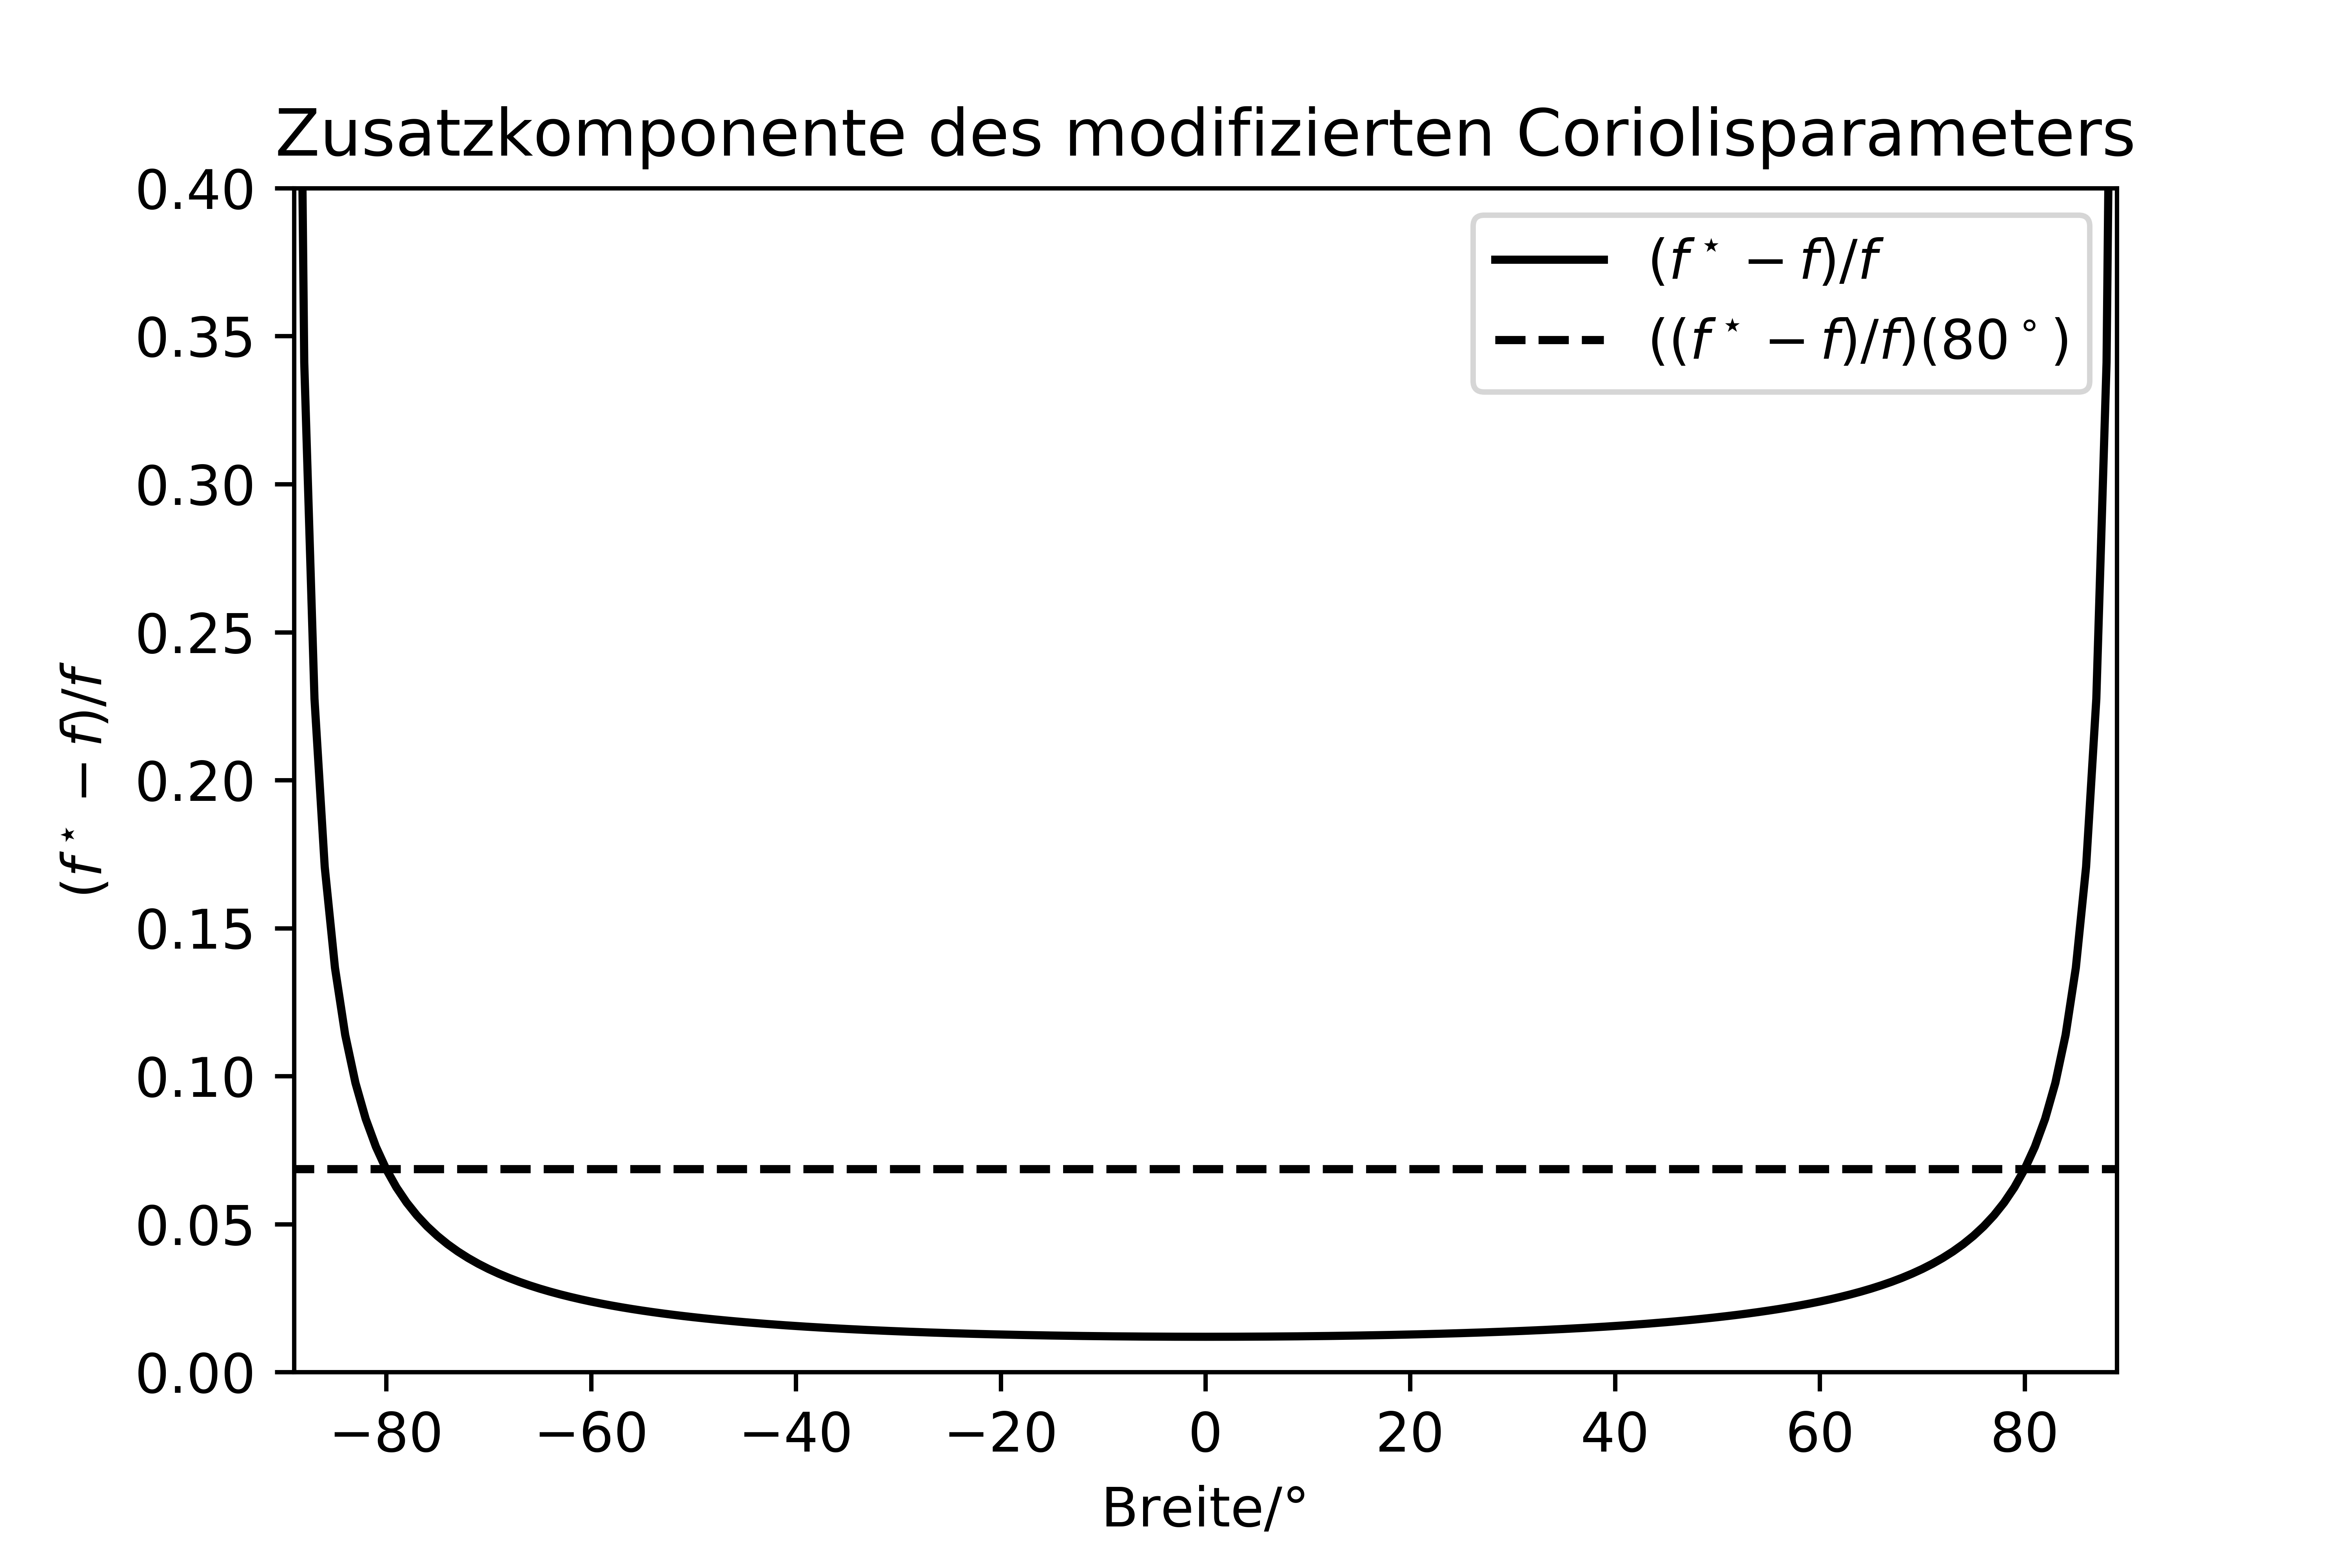
\includegraphics[width = 0.6\textwidth]{figs/f_mod}
\caption{Die Zusatzkomponente von $f^\star$ als Funktion der Breite. Der Wert bei $\varphi = \pm 85^\circ$ ist zusätzlich eingetragen. Es wurde von einer Windgeschwindigkeit von $u = 10$ m/s ausgegangen.}
\label{fig:coriolis_mod}
\end{center}
\end{figure}

Alle bisher gemachten Näherungen sind global anwendbar. Bei der in diesem Abschnitt gemachten Approximation ist dies nicht mehr der Fall. Man definiert den modifizierten Coriolis-Parameter $f^\star$ durch
%
\begin{align}
f^\star \coloneqq f\left(1 + \frac{u}{2a\omega\cos\left(\varphi\right)}\right)\label{eq:f_mod}.
\end{align}
%
$f^\star$ ist dabei, anders als $f$, auch vom Geschwindigkeitsfeld abhängig und beschreibt nicht mehr nur die Coriolis-Kraft. Damit lassen sich die Glg.en \eqref{eq:x_momentum_simplified} - \eqref{eq:y_momentum_simplified} kürzer notieren als
%
\begin{align}
\frac{\partial u}{\partial t} + u\frac{\partial u}{\partial x} + v\frac{\partial u}{\partial y} + w\frac{\partial u}{\partial z} & = -\frac{1}{\rho}\frac{\partial p}{\partial x} + f^\star v + F_{R,x}
\label{eq:x_momentum_simplified_shallow_mod},\\
\frac{\partial v}{\partial t} + u\frac{\partial v}{\partial x} + v\frac{\partial v}{\partial y} + w\frac{\partial v}{\partial z} & = -\frac{1}{\rho}\frac{\partial p}{\partial y} - f^\star u + F_{R,y}
\label{eq:y_momentum_simplified_shallow_mod}.
\end{align}
%
Für die meisten dynamischen Überlegungen kann man, zumindest bis in Breiten von 80 Grad, von $f^\star = f$ ausgehen. Dies wird in Abb. \ref{fig:coriolis_mod} veranschaulicht. Damit erhält man folgende vereinfachte horizontale Bewegungsgleichungen:
%
\begin{center}
\doublebox{\parbox{0.8\textwidth}{
\begin{center}
\begin{align}
\frac{\partial u}{\partial t} + u\frac{\partial u}{\partial x} + v\frac{\partial u}{\partial y} + w\frac{\partial u}{\partial z} & = -\frac{1}{\rho}\frac{\partial p}{\partial x} + fv + F_{R,x}
\label{eq:x_momentum_simplified_simplified}\\
\frac{\partial v}{\partial t} + u\frac{\partial v}{\partial x} + v\frac{\partial v}{\partial y} + w\frac{\partial v}{\partial z} & = -\frac{1}{\rho}\frac{\partial p}{\partial y} - fu + F_{R,y}
\label{eq:y_momentum_simplified_simplified}
\end{align}
\end{center}
}}
\end{center}

\section{Pseudo-inkompressible Approximation}
\label{sec:pseudo-inkompressible_approximation}\index{pseudo-inkompressible Approximation}\index{Approximation!pseudo-inkompressible}

Die sogenannte \textit{pseudo-inkompressible Approximation} wurde in \cite{10.1175/1520-04691989046<1453:ITAA>2.0.CO;2} vorgestellt. Um sie zu begründen, betrachtet man zunächst die Gleichungen der shallow atmosphere in der in Absch. \ref{sec:potentielle_temperatur_als_prognostische_variable_hamilton} Form
%
\begin{align}
\md{u} & = -c^{(p)}\theta\frac{\partial\Pi}{\partial x} + fv,\\
\md{v} & = -c^{(p)}\theta\frac{\partial\Pi}{\partial y} - fu,\\
\md{w} & = -c^{(p)}\theta\frac{\partial\Pi}{\partial z} - g,\\
\md{\rho} & = -\rho\nabla\cdot\mathbf{v},\\
\md{\Pi} & \stackrel{\text{Glg. \eqref{eq:exner-pressure_material_derivative}}}{=} -\frac{R_d\Pi}{c^{(v)}}\nabla\cdot\mathbf{v}.\label{eq:pseudo-inc_deriv_0}
\end{align}
%
Modifiziert wird nun lediglich Glg. \eqref{eq:pseudo-inc_deriv_0}. Hierzu führt man einen Hintergrundzustand $\left(\newoverline{\Pi}\left(z\right), \newoverline{\theta}\left(z\right)\right)$ ein, Abweichungen hiervon werden wie üblich mit gestrichenen Größen bezeichnet. Damit lässt sich Glg. \eqref{eq:pseudo-inc_deriv_0} unter der Annahme $\Pi' \ll \newoverline{\Pi}$ in der Form
%
\begin{align}
\md{\Pi'} + w\frac{d\newoverline{\Pi}}{dz} + \frac{R_d\newoverline{\Pi}}{c^{(v)}}\nabla\cdot\mathbf{v} & = 0\\
\Leftrightarrow \frac{c^{(v)}}{R_d\Pi}\md{\Pi'} + \frac{c^{(v)}}{R_d\newoverline{\Pi}}w\frac{d\newoverline{\Pi}}{dz} + \nabla\cdot\mathbf{v} & = 0\label{eq:pseudo-inc_deriv_1}
\end{align}
%
notieren. Die pseudo-inkompressible Approximation\index{pseudo-inkompressible Approximation}\index{Approximation!pseudo-inkompressible} beruht nun darauf, in Glg. \eqref{eq:pseudo-inc_deriv_1} den Term $\frac{c^{(v)}}{R_d\Pi}\md{\Pi}$ zu vernachlässigen, also von
%
\begin{align}
\frac{c^{(v)}}{R_d\newoverline{\Pi}}w\frac{d\newoverline{\Pi}}{dz} + \nabla\cdot\mathbf{v} = 0\label{eq:pseudo-inc_deriv_2}
\end{align}
%
auszugehen. Der Hintergrundzustand erfüllt die Zustandsgleichung in der Form Glg. \eqref{eq:exner_pressure_diag}:
%
\begin{align}
\newoverline{\Pi} & = \left(\frac{R_d\newoverline{\rho}\newoverline{\theta}}{p_0}\right)^{R_d/c^{(v)}}
\end{align}
%
Hieraus folgt mittels der Kettenregel
%
\begin{align}
\frac{d\newoverline{\Pi}}{dz} = \newoverline{\Pi}\frac{R_d}{c^{(v)}\newoverline{\rho}\newoverline{\theta}}\frac{d\left(\newoverline{\rho}\newoverline{\theta}\right)}{dz}.
\end{align}
%
Setzt man dies in Glg. \eqref{eq:pseudo-inc_deriv_2} ein, erhält man
%
\begin{align}
	w\frac{d\left(\newoverline{\rho}\newoverline{\Pi}\right)}{dz} + \newoverline{\rho}\newoverline{\theta}\nabla\cdot\mathbf{v} = 0
\end{align}
%
Dies führt auf die kompakte Formulierung
%
\begin{center}
\doublebox{\parbox{0.8\textwidth}{
\begin{center}
\begin{align}
\nabla\cdot\left(\newoverline{\rho}\newoverline{\theta}\mathbf{v}\right) & = 0
\end{align}
\end{center}
}}
\end{center}
%
der pseudo-inkompressiblen Approximation\index{pseudo-inkompressible Approximation}\index{Approximation!pseudo-inkompressible}.

\section{Anelastische Approximation}
\label{sec:anelastische_approximation}\index{anelastische Approximation}\index{Approximation!anelastische}

In der sogenannten \textit{anelastischen Approximation}\index{anelastische Approximation}\index{Approximation!anelastische} schreibt man die thermodynamischen Größen in der Form
%
\begin{align}
\rho\left(\varphi, \lambda, z, t\right) & = \rho_0\left(z\right) + \rho'\left(\varphi, \lambda, z, t\right),\label{eq:anelastic_deriv_0}\\
p\left(\varphi, \lambda, z, t\right) & = p_0\left(z\right) + p'\left(\varphi, \lambda, z, t\right),\label{eq:anelastic_deriv_1}\\
\theta\left(\varphi, \lambda, z, t\right) & = \theta_0 + \theta'\left(\varphi, \lambda, z, t\right).\label{eq:anelastic_deriv_2}
\end{align}
%
Der Hintergrundzustand $\left(\rho_0, p_0, \theta_0\right)$ sei isentrop und hydrostatisch balanciert,
%
\begin{align}
\frac{dp_0}{dz} = -g\rho_0.\label{eq:anelastic_deriv_4}
\end{align}
%
Die unapproximierten reversiblen Gleichungen lauten
%
\begin{align}
\rho\md{\mathbf{v}} & = -\nabla p - \rho\mathbf{f}\times\mathbf{v} + \rho\mathbf{g},\\
\frac{\partial\rho}{\partial t} + \nabla\cdot\left(\rho\mathbf{v}\right) & = 0,\\
	\md{\theta} & = 0.\label{eq:anelastic_deriv_5}
\end{align}
%
Setzt man hier die Gleichungen \eqref{eq:anelastic_deriv_0} - \eqref{eq:anelastic_deriv_2} ein. erhält man
%
\begin{align}
\left(\rho_0 + \rho'\right)\md{\mathbf{v}} & = -\nabla\left(p_0 + p'\right) - \left(\rho_0 + \rho'\right)\mathbf{f}\times\mathbf{v} + \left(\rho_0 + \rho'\right)\mathbf{g},\\
\frac{\partial\rho'}{\partial t} + \nabla\cdot\left[\left(\rho_0 + \rho'\right)\mathbf{v}\right] & = 0,\\
\md{\theta'} & = 0.
\end{align}
%
Das anelastische Gleichungssystem\index{anelastisches Gleichungssystem}\index{Gleichungssystem!anelastisches} wird genau wie das inkompressible häufig verwendet, um atmosphärische tiefe Konvektion\index{tiefe Konvektion}\index{Konvektion!tiefe} zu untersuchen.

\subsection{Horizontale Impulsgleichung}
\label{sec:horizontale_impulsgleichung}\index{horizontale Impulsgleichung!anelastische Approximation}\index{Impulsgleichung!horizontale!anelastische Approximation}

Ersetzt man im Vorfaktor der Beschleunigung (inklusive der Coriolis-Beschleunigung\index{Coriolis-Beschleunigung}) die Dichte durch ihren Mittelwert, erhält man
%
\begin{align}
\rho_0\md{\mathbf{v}} & = -\nabla\left(p_0 + p'\right) - \rho_0\mathbf{f}\times\mathbf{v} + \left(\rho_0 + \rho'\right)\mathbf{g}\nonumber\\
\Leftrightarrow \md{\mathbf{v}} & = -\frac{1}{\rho_0}\nabla\left(p_0 + p'\right) - \mathbf{f}\times\mathbf{v} + \frac{\rho_0 + \rho'}{\rho_0}\mathbf{g}\nonumber\\
\Leftrightarrow \md{\mathbf{v}} & = -\nabla\Phi - \mathbf{f}\times\mathbf{v} + \frac{\rho_0 + \rho'}{\rho_0}\mathbf{g}\label{eq:anelastic_deriv_3}
\end{align}
%
mit
%
\begin{align}
\Phi \coloneqq \frac{p'}{\rho_0}
\end{align}
%
Mit der shallow-atmosphere-Approximation\index{shallow atmosphere} erhält man die Komponenten der horizontalen Impulsgleichung in der Form
%
\begin{center}
\doublebox{\parbox{0.8\textwidth}{
\begin{center}
\begin{align}
\md{u} & = -\frac{\partial\Phi}{\partial x} + fv,\\
\md{v} & = -\frac{\partial\Phi}{\partial y} - fu.
\end{align}
\end{center}
}}
\end{center}

\subsection{Vertikale Impulsgleichung}
\label{sec:vertikale_impulsgleichung}\index{vertikale Impulsgleichung!anelastische Approximation}\index{Impulsgleichung!vertikale!anelastische Approximation}

Projiziert man Glg. \eqref{eq:anelastic_deriv_3} auf $\mathbf{k}$, erhält man
%
\begin{align}
\md{w} & = -\frac{1}{\rho_0}\frac{\partial\left(p_0 + p'\right)}{\partial z} - \frac{\rho_0 + \rho'}{\rho_0}g\nonumber\\
\Leftrightarrow \md{w} & = -\frac{1}{\rho_0}\frac{\partial p_0}{\partial z} - g - \frac{1}{\rho_0}\frac{\partial p'}{\partial z} - \frac{\rho'}{\rho_0}g\nonumber\\
\Leftrightarrow \md{w} & \stackrel{\text{Glg. \eqref{eq:anelastic_deriv_4}}}{=} -\frac{1}{\rho_0}\frac{\partial p'}{\partial z} - \frac{\rho'}{\rho_0}g\nonumber\\
\Leftrightarrow \md{w} & = -\frac{\partial\Phi}{\partial z} - \frac{\Phi}{\rho_0}\frac{d\rho_0}{dz} - \frac{\rho'}{\rho_0}g\nonumber\\
	\Leftrightarrow \md{w} & = -\frac{\partial\Phi}{\partial z} - \frac{p'}{\rho_0^2}\frac{d\rho_0}{dz} - \frac{\rho'}{\rho_0}g.\label{eq:anelastic_deriv_6}
\end{align}
%
Für die Hintergrundtemepratur $T_0 = T_0\left(z\right)$ als Funktion der Höhe gilt
%
\begin{align}
	T_0\left(z\right) = \theta_0\left(\frac{p_0}{p_\text{ref}}\right)^{R_d/c^{(p)}}.
\end{align}
%
Für die Hintergrunddichte $\rho_0 = \rho_0\left(z\right)$ gilt mit der thermischen Zustandsgleichung idealer Gase
%
\begin{align}
	\rho_0\left(z\right) = \frac{p_0}{R_dT_0} = \frac{p_0}{R_d\theta_0}\left(\frac{p_\text{ref}}{p_0}\right)^{R_d/c^{(p)}}.\label{eq:anelastic_deriv_7}
\end{align}
%
Hieraus folgt
\begin{align}
	\frac{d\rho_0}{dz} = \rho_0\frac{1 - \frac{R_d}{c^{(p)}}}{p_0}\frac{dp_0}{dz} = -\rho_0\frac{1 - \frac{R_d}{c^{(p)}}}{p_0}g\rho_0 = -\frac{c^{(p)} - c^{(p)} + c^{(v)}}{c^{(p)}p_0}g\rho_0^2 = -\frac{c^{(v)}}{c^{(p)}p_0}g\rho_0^2 = -\frac{g\rho_0^2}{\kappa p_0}.
\end{align}
%
Setzt man dies in Glg. \eqref{eq:anelastic_deriv_6} ein, erhält man
%
\begin{align}
\md{w} & = -\frac{\partial\Phi}{\partial z} + \frac{gp'}{\kappa p_0} - \frac{\rho'}{\rho_0}g = -\frac{\partial\Phi}{\partial z} + g\left(\frac{p'}{\kappa p_0} - \frac{\rho'}{\rho_0}\right). 
\end{align}
%
Aus Glg. \eqref{eq:anelastic_deriv_7} folgt
%
\begin{align}
	\theta\left(\rho, p\right) = \frac{p}{R_d\rho}\left(\frac{p_\text{ref}}{p}\right)^{R_d/c^{(p)}}.
\end{align}
%
Entwickelt man dies in erster Ordnung um $\left(\rho_0, p_0\right)$, erhält man
%
\begin{align}
	\theta \approx \theta_0\left(1 - \frac{\rho'}{\rho_0} + \frac{p'}{\kappa p_0}\right) \Rightarrow \theta' \approx \theta_0\left(-\frac{\rho'}{\rho_0} + \frac{p'}{\kappa p_0}\right). 
\end{align}
%
Somit gilt unter Vernachlässigung des Ungefähr-Zeichens
%
\begin{align}
	g\left(\frac{p'}{\kappa p_0} - \frac{\rho'}{\rho_0}\right) = g\frac{\theta'}{\theta_0}.
\end{align}
%
Definiert man die Buoyancy\index{Buoyancy} $b$ durch
%
\begin{align}
b \coloneqq g\frac{\theta'}{\theta_0},
\end{align}
%
so lautet die vertikale Impulsgleichung\index{vertikale Impulsgleichung!anelastische Approximation}\index{Impulsgleichung!vertikale!anelastische Approximation}\index{anelastische Approximation!vertikale Impulsgleichung} der anelastischen Approximation
%
\begin{center}
\doublebox{\parbox{0.8\textwidth}{
\begin{center}
\begin{align}
\md{w} = -\frac{\partial\Phi}{\partial z} + b.
\end{align}
\end{center}
}}
\end{center}

\subsection{Temperaturgleichung}
\label{sec:temperaturgleichung_anleastische_approximation}\index{Temperaturgleichung!anelastische Approximation}\index{anelastische Approximation!Temperaturgleichung}

Die Buoyancy $b$ ist nur eine Funktion der potentiellen Temperatur $\theta$, somit folgt aus Glg. \eqref{eq:anelastic_deriv_5}

\begin{center}
\doublebox{\parbox{0.8\textwidth}{
\begin{center}
\begin{align}
\md{b} = 0.
\end{align}
\end{center}
}}
\end{center}

\subsection{Kontinuitätsgleichung}
\label{sec:kontinuitätsgleichung_anleastische_approximation}\index{Kontinuitätsgleichung!anelastische Approximation}\index{Kontinuitätsgleichung!vertikale!anelastische Approximation}

Setzt man Glg. \eqref{eq:anelastic_deriv_0} in die Kontinuitätsgleichung ein, erhält man
%
\begin{align}
	\frac{\partial \rho'}{\partial t} + \nabla\cdot\left[\left(\rho_0 + \rho'\right)\mathbf{v}\right] = 0.
\end{align}
%
Vernachlässigt man hier die Schwankung $\rho'$, erhält man
%
\begin{center}
\doublebox{\parbox{0.8\textwidth}{
\begin{center}
\begin{align}
	\nabla\cdot\left(\rho_0\mathbf{v}\right) = 0.
\end{align}
\end{center}
}}
\end{center}

\subsection{Zusammenstellung}
\label{sec:zusammenstellung}

Das anelastische Gleichungssystem\index{anelastisches Gleichungssystem}\index{Gleichungssystem!anelastisches} lautet zusammenfassend

\begin{center}
\doublebox{\parbox{0.8\textwidth}{
\begin{center}
\begin{align}
\md{u} & = -\frac{\partial\Phi}{\partial x} + fv,\\
\md{v} & = -\frac{\partial\Phi}{\partial y} - fu,\\
\md{w} & = -\frac{\partial\Phi}{\partial z} + b,\\
\md{b} & = 0,\\
\nabla\cdot\left(\rho_0\mathbf{v}\right) & = 0.
\end{align}
\end{center}
}}
\end{center}

\section{Boussinesq-Approximation}
\label{sec:boussinesq-approximation}\index{Boussinesq-Approximation}

In \cite{1960ApJ...131..442S} wurde die sogenannte \textit{Boussinesq-Approximation}\index{Boussinesq-Approximation} für ein ideales Gas hergeleitet. Sie wird jedoch heutzutage vorwiegend auf den Ozean angemeldet, daher wird die Herleitung in \cite{1960ApJ...131..442S} hier für ein allgemeines Fluid verallgemeinert.

Sei $\psi$ eine der thermodynamischen Zustandsgrößen. Notiere für diese
%
\begin{align}
\psi = \psi\left(\varphi, \lambda, z\right) = \psi_m + \psi_0\left(z\right) + \psi'\left(\varphi, \lambda, z\right),\label{eq:boussinesq_deriv_5}
\end{align}
%
hierbei ist $\psi_m$ der Mittelwert von $\psi$, $\psi_0$ die hydrostatische Schichtung unter Abwesenheit von Bewegung und Beschleunigungen und $\psi'$ die Variation, die durch Bewegung entsteht. Definiere die zu $\psi$ gehörende Skalenhöhe\index{Skalenhöhe} $D_\psi$ durch
%
\begin{align}
D_\psi \coloneqq \left|\frac{1}{\psi_m}\frac{d\psi_0}{dz}\right|^{-1}.
\end{align}
%
Das Fluid habe die Dicke $h$. Der erste Teil der sogenannten \textit{Boussinesq-Approximation}\index{Boussinesq-Approximation}
%
\begin{center}
\doublebox{\parbox{0.8\textwidth}{
\begin{center}
\begin{align}
h \ll \left(D_\psi\right)_\text{min},\label{eq:boussinesq_0}
\end{align}
\end{center}
}}
\end{center}
%
wobei $\left(D_\psi\right)_\text{min}$ die minimale Skalenhöhe\index{Skalenhöhe} aller thermodynamischen Zustandsgrößen bezeichnet. Dies impliziert
%
\begin{align}
\left|\frac{\psi_0}{\psi_m}\right| \ll 1\label{eq:boussinesq_deriv_0}
\end{align}
%
für alle thermodynamischen Variablen. Der zweite Teil der Boussinesq-Approximation\index{Boussinesq-Approximation} lautet
%
\begin{center}
\doublebox{\parbox{0.8\textwidth}{
\begin{center}
\begin{align}
\left|\rho'\right| \leq O\left(\rho_0\right).\label{eq:boussinesq_1}
\end{align}
\end{center}
}}
\end{center}
%
Die Boussinesq-Approximation\index{Boussinesq-Approximation} ist im Ozean gerechtfertigt, in der Atmosphäre jedoch nur für flache Systeme.

Man geht an dieser Stelle von einem homogenen System aus. In diesem Fall kann man die thermische Zustandsgleichung in der Form
%
\begin{align}
\rho = \rho\left(p, T\right)
\end{align}
%
notieren. Dies kann man in eine Taylor-Reihe um den Entwicklungspunkt $\left(p, T\right)^T = \left(p_m, T_m\right)^T$ entwickeln:\footnote{Definiert man $\rho_m, p_m, T_m$ als Mittel der jeweiligen Größen, gilt aufgrund der Nichtlinearität der Zustandsgleichung im Allgemeinen $\rho_m \not= \rho\left(p_m, T_m\right)$. Daher ist es sinnvoll, $\rho_m \coloneqq \rho\left(p_m, T_m\right)$ zu definieren.}
%
\begin{align}
\rho\left(p, T\right) & = \rho_m\big[1 - a_m\left(T - T_m\right) + K_m\left(p - p_m\right) + \frac{1}{2}\left(\frac{1}{\rho}\frac{\partial^2\rho}{\partial T^2}\right)_m\left(T - T_m\right)^2\nonumber\\
&  + \frac{1}{2}\left(\frac{1}{\rho}\frac{\partial^2\rho}{\partial p^2}\right)_m\left(p - p_m\right)^2 + \left(\frac{1}{\rho}\frac{\partial^2\rho}{\partial T\partial p}\right)_m\left(T - T_m\right)\left(p - p_m\right)\nonumber\\
&  + O\left[\left(T - T_m\right)^3, \left(p - p_m\right)^3\right]\big]\label{eq:taylor_eos_boussinesq}
\end{align}
%
Dabei wurden die Definitionen \index{thermischer Expansionskoeffizient}\index{Expansionskoeffizient!thermischer}\index{Kompressibilität}
%
\begin{align}
a_m &\coloneqq -\left[\frac{1}{\rho}\left(\frac{\partial\rho}{\partial T}\right)_p\right]_m\text{(thermischer Expansionskoeffizient)},\\
K_m &\coloneqq \left[\frac{1}{\rho}\left(\frac{\partial\rho}{\partial p}\right)_T\right]_m\text{(Kompressibilität)}
\end{align}
%
eingesetzt. Für diese Größen kann man für Fluide
%
\begin{align}
a_m \ll -\frac{1}{\rho_m}\frac{-\rho_m}{T_m} = \frac{1}{T_m}, && K_m \ll \frac{1}{\rho_m}\frac{\rho_m}{p_m} = \frac{1}{p_m}\label{eq:boussinesq_deriv_3}
\end{align}
%
abschätzen. Setzt man dies in Glg. \eqref{eq:taylor_eos_boussinesq} auch für die zweiten Ableitungen ein, erhält man unter Vernachlässigung der Terme dritter und höherer Ordnung
%
\begin{align}
\frac{\rho - \rho_m}{\rho_m} \ll -\frac{T - T_m}{T_m} + \frac{p - p_m}{p_m} \pm \frac{\left(T - T_m\right)^2}{T_m^2} \pm \frac{\left(p - p_m\right)^2}{p_m^2}.
\end{align}
%
Aufgrund von Glg.en \eqref{eq:boussinesq_deriv_0} und \eqref{eq:boussinesq_1} kann man die rechte Seite durch
%
\begin{align}
-\frac{T - T_m}{T_m} + \frac{p - p_m}{p_m} \pm \frac{\left(T - T_m\right)^2}{T_m^2} \pm \frac{\left(p - p_m\right)^2}{p_m^2} \approx -\frac{T - T_m}{T_m} + \frac{p - p_m}{p_m}
\end{align}
%
nähern. Es gilt also unter Vernachlässigung des Ungefähr-Zeichens (in erster Ordnung in den Störungen $\psi - \psi_m$ der thermodynamischen Variablen $\psi$)
%
\begin{align}
\frac{\rho - \rho_m}{\rho_m} = -a_m\left(T - T_m\right) + K_m\left(p - p_m\right).\label{eq:boussinesq_deriv_6}
\end{align}
%
Dies impliziert
%
\begin{align}
\rho_0 & = \rho_m\left(-a_mT_0 + K_mp_0\right),\\
\rho' & = \rho_m\left(-a_mT' + K_mp'\right).\label{eq:boussinesq_deriv_2}
\end{align}

\subsection{Impulsgleichung}
\label{sec:impulsgleichung_boussinesq}\index{Boussinesq-Approximation!Impulsgleichung}\index{Impulsgleichung!Boussinesq-Approximation}

Die hydrostatische Grundgleichung\index{hydrostatische Grundgleichung}\index{Grundgleichung!hydrostatische} \eqref{eq:hydrostatic} lautet
%
\begin{align}
\frac{dp_0}{dz} = -g\rho_m - g\rho_0.\label{eq:boussinesq_hydrostat}
\end{align}
%
Setzt man dies in die Impulsgleichung ein, erhält man
%
\begin{align}
\rho\left(\frac{\partial}{\partial t} + \mathbf{v}\cdot\nabla\right)\mathbf{v} & = -\nabla p' - \frac{dp_0}{dz}\mathbf{k} - g\rho\mathbf{k} - \rho\mathbf{f}\times\mathbf{v} + \rho\mathbf{f}_R\nonumber\\
& = -\nabla p' - \frac{dp_0}{dz}\mathbf{k} - g\rho_m\mathbf{k} - g\rho_0\mathbf{k} - g\rho'\mathbf{k} - \rho\mathbf{f}\times\mathbf{v} + \rho\mathbf{f}_R\nonumber\\
& = -\nabla p' - g\rho'\mathbf{k} - \rho\mathbf{f}\times\mathbf{v} + \rho\mathbf{f}_R.
\end{align}
%
Dividiert man dies durch $\rho_m$, erhält man
%
\begin{align}
\frac{\rho}{\rho_m}\left(\frac{\partial}{\partial t} + \mathbf{v}\cdot\nabla\right)\mathbf{v} & = -\frac{1}{\rho_m}\nabla p' - g\frac{\rho'}{\rho_m}\mathbf{k} - \frac{\rho}{\rho_m}\mathbf{f}\times\mathbf{v} + \frac{\rho}{\rho_m}\mathbf{f}_R.
\end{align}
%
Aufgrund von Glg. \eqref{eq:boussinesq_deriv_0} kann man
%
\begin{align}
\frac{\rho}{\rho_m} \approx 1\label{eq:boussinesq_deriv_1}
\end{align}
%
nähern. Dies führt auf
%
\begin{center}
\doublebox{\parbox{0.8\textwidth}{
\begin{center}
\begin{align}
\left(\frac{\partial}{\partial t} + \mathbf{v}\cdot\nabla\right)\mathbf{v} & = -\frac{1}{\rho_m}\nabla p' - g\frac{\rho'}{\rho_m}\mathbf{k} - \mathbf{f}\times\mathbf{v} + \mathbf{f}_R.\label{eq:boussinesq_momentum_0}
\end{align}
\end{center}
}}
\end{center}
%
Die Kontinuitätsgleichung lautet
%
\begin{align}
\left(\frac{\partial}{\partial t} + \mathbf{v}\cdot\nabla\right)\rho = -\rho\nabla\cdot\mathbf{v}.
\end{align}
%
Dividiert man dies durch $\rho_m$, erhält man
%
\begin{align}
\left(\frac{\partial}{\partial t} + \mathbf{v}\cdot\nabla\right)\frac{\rho - \rho_m}{\rho_m} = -\frac{\rho}{\rho_m}\nabla\cdot\mathbf{v}.
\end{align}
%
Setzt man hier Glg. \eqref{eq:boussinesq_deriv_0} ein, erhält man
%
\begin{center}
\doublebox{\parbox{0.8\textwidth}{
\begin{center}
\begin{align}
\nabla\cdot\mathbf{v} = 0 \Leftrightarrow \md{\rho} = 0.
\end{align}
\end{center}
}}
\end{center}
%
Unter der Boussinesq-Approximation\index{Boussinesq-Approximation} vereinfacht sich die Kontinuitätsgleichung also auf ihre inkompressible Form.

Man kann die Impulsgleichung\index{Impulsgleichung!Boussinesq-Approximation}\index{Boussinesq-Approximation!Impulsgleichung} Glg. \eqref{eq:boussinesq_momentum_0} noch etwas vereinfachen. Die vertikale Komponente dieser Gleichung lautet
%
\begin{align}
\left(\frac{\partial}{\partial t} + \mathbf{v}\cdot\nabla\right)w & = -\frac{1}{\rho_m}\frac{\partial p'}{\partial z} - g\frac{\rho'}{\rho_m} - \left(\mathbf{f}\times\mathbf{v}\right)\cdot\mathbf{k} + \mathbf{f}_R\cdot\mathbf{k}.
\end{align}
%
Für Druckgradient und Schwere erhält man mit Glg. \eqref{eq:boussinesq_deriv_2}
%
\begin{align}
-\frac{1}{\rho_m}\frac{\partial p'}{\partial z} - g\frac{\rho'}{\rho_m} & = -\frac{1}{\rho_m}\frac{\partial p'}{\partial z} - g\left(-a_mT' + K_mp'\right) = -\frac{1}{\rho_m}\frac{\partial p' }{\partial z} - gK_mp' + ga_mT'\nonumber\\
& = -\frac{1}{\rho_m}\left(\frac{\partial p' }{\partial z} + g\rho_mK_mp'\right) + ga_mT' = -\frac{1}{\rho_m}\left(\frac{\partial p' }{\partial z} + \frac{p'}{H}\right) + ga_mT'\label{eq:boussinesq_deriv_4}
\end{align}
%
mit
%
\begin{align}
H \coloneqq \frac{1}{g\rho_mK_m}.
\end{align}
%
Mit Glg. \eqref{eq:boussinesq_deriv_3} kann man
%
\begin{align}
H = \frac{1}{g\rho_m}\frac{1}{K_m} \gg \frac{1}{g\rho_m}p_m =: H'
\end{align}
%
abschätzen. $H'$ ist die Dicke eines Fluides der homogenen Dichte $\rho_m$, welches hydrostatisch im Schwerefeld $g$ ruht und in dem der Druck linear von oben nach unten von Null auf $p_m$ zunimmt. Man kann
%
\begin{align}
H' \sim \frac{h}{2}
\end{align} 
%
abschätzen, also gilt auch
%
\begin{align}
H \gg h.
\end{align}
%
Dies bedeutet, dass man in Glg. \eqref{eq:boussinesq_deriv_4}
%
\begin{align}
\frac{\partial p' }{\partial z} + \frac{p'}{H} \approx \frac{\partial p'}{\partial z}
\end{align}
%
nähern kann. Dies führt auf eine vereinfachte Form von Glg. \eqref{eq:boussinesq_momentum_0}:
%
\begin{center}
\doublebox{\parbox{0.8\textwidth}{
\begin{center}
\begin{align}
\left(\frac{\partial}{\partial t} + \mathbf{v}\cdot\nabla\right)\mathbf{v} & = -\frac{1}{\rho_m}\nabla p' + ga_mT'\mathbf{k} - \mathbf{f}\times\mathbf{v} + \mathbf{f}_R
\end{align}
\end{center}
}}
\end{center}

\subsection{Temperaturgleichung}
\label{sec:temperaturgleichung}\index{Boussinesq-Approximation!Temperaturgleichung}\index{Temperaturgleichung!Boussinesq-Approximation}

Multipliziert man Glg. \eqref{eq:td1_ideal_gas} mit der Dichte $\rho$, erhält man

\begin{align}
\rho c^{(v)}\md{T} - \frac{p}{\rho}\md{\rho} = q^{(V)},\label{eq:boussineq_t_deriv_0}
\end{align}
%
wobei $q^{(V)}$ die Wärmeleistungsdichte ist. Aufgrund von Glg. \eqref{eq:boussinesq_deriv_5} gilt
%
\begin{align}
\md{T} = \frac{\partial T}{\partial t} + \mathbf{v}\cdot\nabla T = \frac{\partial T'}{\partial t} + \mathbf{v}\cdot\nabla T.
\end{align}
%
Setzt man dies in Glg. \eqref{eq:boussineq_t_deriv_0} ein, erhält man
%
\begin{align}
\rho_mc^{(v)}\left(\frac{\partial T'}{\partial t} + \mathbf{v}\cdot\nabla T\right) - \frac{p}{\rho}\md{\rho} = q^{(V)},\label{eq:boussinesq_deriv_7}
\end{align}
%
wobei im Vorfaktor der Temperaturtendenz die Dichte $\rho$ durch die mittlere Dichte $\rho_m$ ersetzt wurde. Den Kompressionsterm kann man in erster Ordnung in den Abweichungen von den gemittelten Größen zu
%
\begin{align}
-\frac{p}{\rho}\md{\rho} \approx -\frac{p_m}{\rho_m}\md{\rho} = -\frac{p_m}{\rho_m}\left(\frac{\partial\rho}{\partial t} + \mathbf{v}\cdot\nabla\rho\right)
\end{align}
%
vereinfachen. Mit Glg. \eqref{eq:boussinesq_deriv_6} folgt unter Vernachlässigung des Ungefähr-Zeichens
%
\begin{align}
-\frac{p}{\rho}\md{\rho} \approx -\frac{p_m}{\rho_m}\left(\frac{\partial\rho}{\partial t} + \mathbf{v}\cdot\nabla\rho\right) = -p_m\left(\frac{\partial}{\partial t} + \mathbf{v}\cdot\nabla\right)\left[-a_m\left(T - T_m\right) + K_m\left(p - p_m\right)\right].
\end{align}
%
Um hier die Zeitabhängigkeit des Drucks zu eliminieren, nähert man weiter
%
\begin{align}
-\frac{p}{\rho}\md{\rho} & \approx -p_m\left(\frac{\partial}{\partial t} + \mathbf{v}\cdot\nabla\right)\left[-a_m\left(T - T_m\right) + K_m\left(p - p_m\right)\right]\nonumber\\
& = -p_m\left(\frac{\partial}{\partial t} + \mathbf{v}\cdot\nabla\right)\left[-a_m\left(T_0 + T'\right) + K_mp_0\right]\nonumber\\
& = p_m\left(\frac{\partial}{\partial t} + \mathbf{v}\cdot\nabla\right)a_mT' + p_mwa_m\frac{dT_0}{dz} - p_mK_mw\frac{dp_0}{dz}.
\end{align}
%
Laut Glg. \eqref{eq:boussinesq_hydrostat} gilt in erster Ordnung in der Abweichung von der mittleren Dichte
%
\begin{align}
\frac{dp_0}{dz} \approx -g\rho_m.
\end{align}
%
Somit gilt unter Vernachlässigung des Ungefähr-Zeichens
%
\begin{align}
-\frac{p}{\rho}\md{\rho} & = p_m\left(\frac{\partial}{\partial t} + \mathbf{v}\cdot\nabla\right)a_mT' + p_mwa_m\frac{dT_0}{dz} - p_mK_mw\frac{dp_0}{dz}\nonumber\\
& = p_m\left(\frac{\partial}{\partial t} + \mathbf{v}\cdot\nabla\right)a_mT' + p_mwa_m\frac{dT_0}{dz} + p_mK_mwg\rho_m.
\end{align}
%
Setzt man dies in Glg. \eqref{eq:boussinesq_deriv_7} ein, erhält man
%
\begin{align}
&  \rho_mc^{(v)}\left(\frac{\partial T'}{\partial t} + \mathbf{v}\cdot\nabla T\right) - \frac{p}{\rho}\md{\rho} = q^{(V)}\nonumber\\
&  \rho_mc^{(v)}\left(\frac{\partial T'}{\partial t} + \mathbf{v}\cdot\nabla T\right) + p_m\left(\frac{\partial}{\partial t} + \mathbf{v}\cdot\nabla\right)a_mT' + p_mwa_m\frac{dT_0}{dz} + p_mK_mwg\rho_m = q^{(V)}\nonumber\\
&  \left(\rho_mc^{(v)} + p_ma_m\right)\left(\frac{\partial T'}{\partial t} + \mathbf{v}\cdot\nabla T'\right) + w\left(p_ma_m + \rho_mc^{(v)}\right)\frac{dT_0}{dz} + p_mK_mwg\rho_m = q^{(V)}
\end{align}
%
Dies ist die Temperaturgleichung\index{Boussinesq-Approximation!Temperaturgleichung}\index{Temperaturgleichung!Boussinesq-Approximation} der Boussinesq-Approximation:
%
\begin{center}
\doublebox{\parbox{0.95\textwidth}{
\begin{center}
\begin{align}
\left(c^{(v)} + \frac{p_ma_m}{\rho_m}\right)\left(\frac{\partial T'}{\partial t} + \mathbf{v}\cdot\nabla T'\right) + w\left[\left(\frac{p_ma_m}{\rho_m} + c^{(v)}\right)\frac{dT_0}{dz} + p_mK_mg\right] = \frac{q^{(V)}}{\rho_m}
\end{align}
\end{center}
}}
\end{center}
%
Im idealen Gas gelten
%
\begin{align}
a_m & = -\left[\frac{1}{\rho}\left(\frac{\partial\rho}{\partial T}\right)_p\right]_m = \frac{p_m}{R_s\rho T_m^2} = \frac{\rho_mR_sT_m}{R_s\rho_mT_m^2} = \frac{1}{T_m},\\
K_m & = \left[\frac{1}{\rho}\left(\frac{\partial\rho}{\partial p}\right)_T\right]_m = \frac{1}{\rho_m}\frac{1}{R_sT_m} = \frac{1}{p_m}.
\end{align}
%
Hieraus folgt
%
\begin{align}
\left(c^{(v)} + R_s\right)\left(\frac{\partial T'}{\partial t} + \mathbf{v}\cdot\nabla T'\right) + w\left[\left(R_s + c^{(v)}\right)\frac{dT_0}{dz} + g\right] & = \frac{q^{(V)}}{\rho_m}\nonumber\\
\Leftrightarrow c^{(p)}\left(\frac{\partial T'}{\partial t} + \mathbf{v}\cdot\nabla T'\right) + wc^{(p)}\left(\frac{dT_0}{dz} + g\right) & = \frac{q^{(V)}}{\rho_m}\nonumber\\
\Leftrightarrow\left(\frac{\partial T'}{\partial t} + \mathbf{v}\cdot\nabla T'\right) + w\left(\frac{dT_0}{dz} + \frac{g}{c^{(p)}}\right) & = \frac{q^{(V)}}{c^{(p)}\rho_m}.
\end{align}

\section{Hydrostatik}
\label{sec:hydrostatik}\index{Hydrostatik}

Druckgradient und Schwere sind von der Größenordnung $10$ m/s$^2$, während die Vertikalbeschleunigung in der Größenordnung $10^{-7}$ m/$s^2$ liegt. Die Gleichung
%
\begin{center}
\doublebox{\parbox{0.8\textwidth}{
\begin{center}
\begin{align}
\mathbf{0} = -\frac{1}{\rho}\nabla p + \mathbf{g} \Leftrightarrow \nabla p = \rho\mathbf{g} \stackrel{\substack{\text{radialsymmetrisches}\\\text{Schwerefeld}}}{\Rightarrow} \frac{\partial p}{\partial z} = -g\rho\label{eq:hydrostatic}
\end{align}
\end{center}
}}
\end{center}
%
gilt also auf der synoptischen Skala in ausgezeichneter Näherung, dies ist die \textit{hydrostatische Grundgleichung}.\index{Grundgleichung!hydrostatische}\index{hydrostatische Grundgleichung}

Eine andere Formulierung dieser Gleichung ist $\md{w} = 0$. Die Teilchen haben also eine konstante Vertikalgeschwindigkeit. Diese muss Null sein, da es sonst zum Regelfall wird, dass ein Teilchen im Erdboden oder Weltall verschwindet. Es gilt also die Implikation
%
\begin{align}
\frac{\mathbf{g}}{g}\cdot\nabla p = \rho\mathbf{g} \Rightarrow w = 0.
\end{align}
%
Trotzdem ist es sinnvoll, auch in hydrostatischen Gleichungssystemen eine Vertikalgeschwindigkeit zuzulassen. Dies ist zwar physikalisch widersprüchlich, jedoch nicht mathematisch, da das Gleichungssystem nichts von obiger Folgerung wissen kann. Die Vertikalbewegungen eines solchen Systems entstehen aus der Kontinuitätsgleichung.

Auch wenn man die hydrostatische Annahme nicht macht, kann man einen Grundzustand $\{\newoverline{\alpha}, \newoverline{p}\}$ einführen mit $\alpha \coloneqq \frac{1}{\rho}$ als spezifischem Volumen, der Glg. \eqref{eq:hydrostatic} erfüllt, und die tatsächlichen Größen $\{\alpha, p\}$ als Übelagerung des Grundzustandes mit Abweichungen $\{\alpha', p'\}$ zu notieren, also
%
\begin{align}
\alpha & = \newoverline{\alpha} + \alpha',\\
p & = \newoverline{p} + p'.
\end{align}
%
Dann gilt
%
\begin{align}
-\alpha\nabla p + \mathbf{g} = -\alpha'\nabla\newoverline{p} - \newoverline{\alpha}\nabla p' - \alpha'\nabla p' = -\alpha'\nabla p - \newoverline{\alpha}\nabla p' = -\alpha\nabla p' - ´\alpha'\nabla\newoverline{p}.\label{eq:background_state_prop_0}
\end{align}
%
Das Schwerefeld der Erde hat eine komplizierte Form, der man sich in verschiedenen Stufen annähert. Zunächst geht man davon aus, dass das Schwerefeld radialsymmetrisch ist mit homogenem Betrag des Schwerevektors. Verwendet man anstatt der geometrischen Höhe $z$ die geopotentielle Höhe $\phi = gz$ (dies ist die Energie pro Masse, die nötig ist, um ein Teilchen vom Meeresspiegel auf die Höhe $z$ zu bringen), lautet die hydrostatische Grundgleichung mit der Kettenregel
%
\begin{align}
\frac{\partial p}{\partial\phi} = \frac{\partial p}{\partial z}\frac{\partial z}{\partial\phi} = -\rho.
\end{align}
%
Die SI-Einheit des Geopotentials ist m$^2$/s$^2$. Ein Geopotentialmeter gpm ist definiert durch
%
\begin{align}
1\:\text{gpm} \coloneqq 9,8\:\text{m}^2/\text{s}^2, 
\end{align}
%
sodass
%
\begin{align}
\frac{z}{\text{m}} = \frac{\phi/g}{\text{m}} \approx \frac{\phi}{\text{gpm}}
\end{align}
%
gilt. Möchte man die Höhenabhängigkeit der Schwerebeschleunigung berücksichtigen, so verwendet man hierfür als Formel für das Gravitationspotential zunächst
%
\begin{align}
\phi_g\left(r\right) = -\frac{\phi_0a}{r} + \phi_0
\end{align}
%
mit $\phi_0 \coloneqq GM/a$ mit $G$ als Newton'scher Gravitationskonstante\index{Newton'sche Gravitationskonstante}\index{Gravitationskonstante!Newton'sche} und $M$ als Erdmasse. Dies ist die Formel für das Schwerefeld eines Planeten mit radialsymmatrischer Massenverteilung, sie ergibt sich aus der Formel für eine Punktmasse mit dem Gauß'schen Satz. Bei $r = a$ ist das Potential zu Null normiert. Hieraus folgt
%
\begin{align}
g = \frac{\phi_0a}{r^2} = g_0\frac{a^2}{r^2}
\end{align}
%
mit $g_0 \coloneqq \frac{\phi_0}{a}$. In dieser Approximation fordert man für die generalisierte Vertikalkoordinate geopotentielle Höhe\index{geopotentielle Höhe}\index{Höhe!geopotentielle} $z_g$, dass gilt
%
\begin{align}
g_0z_g\hastobe\phi_g\left(a + z\right) = -\frac{\phi_0a}{a + z} + \phi_0 \Rightarrow z_g = -\frac{a^2}{a + z} + a = \frac{-a^2 + a^2 + za}{a + z} = \frac{z}{1 + \frac{z}{a}}.
\end{align}
%
Hieraus folgt weiterhin
%
\begin{align}
\frac{\partial p}{\partial z} & = \frac{z_g}{z}\frac{\partial p}{\partial z_g} = \left(\frac{1}{1 + \frac{z}{a}} - \frac{z}{a}\frac{1}{\left(1 + \frac{z}{a}\right)^2}\right)\frac{\partial p}{\partial z_g} = \frac{1}{\left(1 + \frac{z}{a}\right)^2}\frac{\partial p}{\partial z_g} = \frac{a^2}{r^2}\frac{\partial p}{\partial z_g} = -g\rho  = -g_0\frac{a^2}{r^2}\rho\nonumber\\
\Rightarrow \frac{\partial p}{\partial z_g} & = -g_0\rho.
\end{align}
%
Verwendet man den Druck als Höhenkoordinate und das Geopotential als die abhängige Koordinate, transformiert man also $p\left(\phi\right)$ auf $\phi\left(p\right)$, so lautet die hydrostatische Grundgleichung
%
\begin{align}
\frac{\partial\phi}{\partial p} = -\alpha\label{eq:hydrostatic_p}
\end{align}
%
mit $\alpha \coloneqq \frac{1}{\rho}$ als dem spezifischen Volumen. Mit der Zustandsgleichung folgt $\alpha = \frac{R_dT}{p}$ in einer trockenen Atmosphäre. Deshalb bezeichnet man $\frac{\partial\phi}{\partial p}$ häufig auch einfach als »Temperatur«.\ Man sieht, dass die Schichtdicke proportional zur Temperatur der Schicht ist. Das dreidimensionale Geopotentialfeld ist also Ausdruck des Bodendrucks und der Temperatur der Luftmassen.

\section{Barotropie}
\label{sec:barotropie}\index{Barotropie}

Von Barotropie spricht man, wenn die Konturflächen des Druckfeldes und des Dichtefeldes gleich sind. In einer trockenen Atmosphäre ist dies gleichbedeutend mit der Tatsache, dass die Temperaturflächen und die Druckflächen gleich sind. In der Realität ist der Baroklinitätswinkel, der den Winkel zwischen $\nabla\rho$ und $\nabla p$ beschreibt, klein. Jedoch ist die vorhandene Baroklinität sehr wichtig für die atmosphärische Dynamik und Barotropie hat weitreichende einschränkende Implikationen.

Leitet man die x-Komponente von Glg. \eqref{eq:x_momentum_simplified_simplified_p} unter Annahme von Barotropie nach $p$ ab, erhält man
%
\begin{align}
\frac{\partial}{\partial p}\md{u} = -\frac{\partial }{\partial p}\frac{\partial\phi}{\partial x} + f\frac{\partial v}{\partial p} = -\frac{\partial }{\partial x}\frac{\partial\phi}{\partial p} + f\frac{\partial v}{\partial p} = f\frac{\partial v}{\partial p}.
\end{align}
%
Es gilt außerdem
%
\begin{align}
\frac{\partial }{\partial p}\md{u} = \frac{\partial}{\partial p}\left(\frac{\partial u}{\partial t} + u\frac{\partial u}{\partial x} + v\frac{\partial u}{\partial y} + \omega\frac{\partial u}{\partial p}\right), 
\end{align}
%
hieraus folgt
%
\begin{align}
\frac{\partial}{\partial t}\frac{\partial u}{\partial p} = \frac{\partial}{\partial p}\frac{\partial u}{\partial t} = f\frac{\partial v}{\partial p} - \frac{\partial}{\partial p}\left(u\frac{\partial u}{\partial x} + v\frac{\partial u}{\partial y} + \omega\frac{\partial u}{\partial p}\right).
\end{align}
%
An dieser Gleichung sieht man, dass, falls die vertikale Scherung global für einen Zeitpunkt verschwindet, dies für alle Zeitpunkte so ist. Verschwindet die vertikale Scherung, sind auch die Horizontaldivergenz und damit nach Glg. \eqref{eq:kont_p} $\frac{\partial\omega}{\partial p}$ höhenkonstant. Das Feld der Vertikalgeschwindigkeit im p-System $\omega = \omega\left( p\right)$ ist also in diesem Fall eine Gerade und eine diagnostische Größe.

\subsection{Flachwassergleichungen}
\label{sec:flachwassergleichungen}\index{Flachwassergleichungen}

Das einfachste Gleichungssystem der Geofluiddynamik mit Zeitableitungen ist das der \textit{Flachwassergleichungen} (SWEs, engl. \textit{shallow water equations}). Um dieses herzuleiten, geht man von den Glg.en \eqref{eq:x_momentum_simplified_simplified} - \eqref{eq:y_momentum_simplified_simplified} aus und nimmt eine homogene Dichte an, außerdem ignoriert man die Reibung. Damit wird die Kontinuitätsgleichung zu
%
\begin{align}
\nabla\cdot\mathbf{v} = 0.
\end{align}
%
Das Fluid habe weiterhin eine Oberfläche, an dieser gelte $p = 0$. Die Tiefe des Mediums sei $h = h\left(x, y, t\right)$ und der Grund habe die z-Koordinate $b = b\left(x, y\right)$. Damit erhält man durch Integration der hydrostatischen Grundgleichung
%
\begin{align}
p\left(z\right) = -\left(0 - p\left(z\right)\right) = -\left(p\left(b + h\right) - p\left(z\right)\right) = -\int_{z}^{b + h}\frac{\partial p}{\partial z}dz = g\rho\int_{z}^{b + h}dz = \left(b + h - z\right)g\rho.
\end{align}
%
Somit folgt
%
\begin{align}
\frac{\partial p}{\partial x} = g\rho \frac{\partial}{\partial x}\left(b + h\right)
\end{align}
%
und analog in y-Richtung. Verschwindet die vertikale Scherung der Horizontalbewegung $\left(\frac{\partial u}{\partial z}, \frac{\partial v}{\partial z}\right)^T$ global zu einem beliebigen Zeitpunkt, so verschwindet auch die lokalzeitliche Tendenz der vertikalen Scherung. Somit ist das Geschwindigkeitsfeld dann zu allen Zeitpunkten höhenunabhängig. Hiervon wird nun ausgegangen. Damit verschwinden die Terme der vertikalen Geschwindigkeitsadvektion. Nun kann man die Kontinuitätsgleichung trivial integrieren:
%
\begin{align}
h\nabla\cdot\mathbf{v} = \int_{b}^{b + h}\nabla\cdot\mathbf{v}dz = -\int_{b}^{b + h}\frac{\partial w}{\partial z}dz = -w\left(b + h\right) + w\left(b\right)\label{eq:swe_deriv_1}
\end{align}
%
Die Annahme, dass die Horizontalgeschwindigkeit nicht geschert ist und die die Integration Glg. \eqref{eq:swe_deriv_1} ermöglicht hat, gibt den Flachwassergleichungen ihren Namen. Bei großen Tiefen kann hiervon nämlich anschaulicherweise nicht mehr ausgegangen werden. In Absch. \ref{sec:sub-poincare-wellen} wird über diese Annahme hinausgegangen. Behandelt man Wellen, so kann man die Flachwassergleichungen verwenden, falls
%
\begin{align}
\text{Wellenlänge} & \gg & \text{Tiefe},\\
\text{Wellenhöhe} & \ll & \text{Tiefe}
\end{align}
%
gelten, was für die Tide (außer in Randmeeren) sowie die Dünung auf offener See der Fall sein kann.

In der Tiefe $b$ gilt die kinematische Randbedingung:
%
\begin{align}
w\left(b\right) & = \frac{dz}{dt}\left(b\right) = \frac{db}{dt} = \mathbf{v}\cdot\nabla_hb
\end{align}
%
An der Oberfläche gilt
%
\begin{align}
w\left(b + h\right) = \md{}\left(b + h\right) = \frac{\partial h}{\partial t} + \mathbf{v}_h\cdot\nabla_h\left(b + h\right).
\end{align}
%
Setzt man dies in Glg. \eqref{eq:swe_deriv_1} ein, erhält man
%
\begin{align}
h\nabla_h\cdot\mathbf{v} & = -\frac{\partial h}{\partial t} - \mathbf{v}\cdot\nabla_h h.
\end{align}
%
Somit erhält man folgendes Gleichungssystem:
%
\begin{center}
\doublebox{\parbox{0.8\textwidth}{
\begin{center}
\begin{align}
\frac{\partial\mathbf{v}}{\partial t} + \left(\mathbf{v}\cdot\nabla\right)\mathbf{v} & = -g\nabla_h\left(h + b\right) - f\left(y\right)\mathbf{k}\times\mathbf{v}\label{eq:swe_0}\\
\frac{\partial h}{\partial t} + \nabla\cdot\left(h\mathbf{v}\right) & = 0\label{eq:swe_1}
\end{align}
\end{center}
}}
\end{center}
%
\subsubsection{Linearisierung}
\label{par:linearisierung}\index{Linearisierung!der Flachwassergleichungen}\index{Flachwassergleichungen!Linearisierung}

Nimmt man einen homogenen Untergrund $b$ an, sowie eine mittlere Tiefe $D$, der eine Störung $d$ überlagert ist, und vernachlässigt alle nichtlinearen Terme, folgt
%
\begin{align}
\frac{\partial\mathbf{v}}{\partial t} & = -g\nabla d - f\mathbf{k}\times\mathbf{v}, \label{eq:flach_lin_1}\\
\frac{\partial d}{\partial t} + D\nabla\cdot\mathbf{v} & = 0.\label{eq:flach_lin_2}
\end{align}

\section{Geostrophie}
\label{sec:geostrophie}\index{Geostrophie}

\renewcommand{\arraystretch}{1.2}
\begin{table}
\centering
\begin{tabular}[h]{|c|c|}
\hline 
\textbf{Term} & \textbf{Größenordnung im SI} \\ 
\hline\hline
$\frac{\partial u}{\partial t}$ & $10^{-4}$ \\ 
\hline 
$u\frac{\partial u}{\partial x}$ & $10^{-4}$ \\ 
\hline 
$fv$ & $10^{-3}$ \\ 
\hline 
$\frac{1}{\rho}\frac{\partial p}{\partial x}$ & $10^{-3}$ \\ 
\hline 
\end{tabular}
\caption{Skalierung der horizontalen Impulsgleichung auf der synoptischen Skala.}
\label{tab:skal_geos}
\end{table}
\renewcommand{\arraystretch}{1}

Für die Rossby-Zahl\index{Rossby-Zahl} $N_\text{Ro}$ gilt
%
\begin{align}
N_\text{Ro} = \frac{U}{Lf} \sim10^{-1}
\end{align}
%
auf der synoptischen Skala. In erster Ordnung liegt also ein Kräftegleichgewicht aus Coriolis-Kraft und Druckgradientkraft vor. Dies ist die geostrophische Approximation. Das entsprechende Windfeld $\mathbf{v}_h = \left(u_g, v_g\right)^T$ erhält man, indem man in den horizontalen Bewegungsgleichungen Glg.en \eqref{eq:x_momentum_simplified_simplified_p} - \eqref{eq:y_momentum_simplified_simplified_p} die Beschleunigung gleich Null setzt.
%
\begin{align}
0 = -\frac{\partial\phi}{\partial x} + fv_g, && 0 = -\frac{\partial\phi}{\partial y} - fu_g
\end{align}
%
Stellt man dies nach der Windgeschwindigkeit um, ergeben sich
%
\begin{align}
v_g = \frac{1}{f}\frac{\partial\phi}{\partial x}, && u_g = -\frac{1}{f}\frac{\partial\phi}{\partial y}.
\end{align}
%
Der geostrophische Wind ist also
%
\begin{center}
\doublebox{\parbox{0.8\textwidth}{
\begin{center}
\begin{align}
\mathbf{v}_{h, g} = \frac{1}{f}\left(\begin{array}{c}
- \frac{\partial\phi}{\partial y}\\
\frac{\partial\phi}{\partial x}\\
\end{array}\right) = \mathbf{k}\times\frac{1}{f}\nabla\phi.
\label{eq:geostr_wind}
\end{align}
\end{center}
}}
\end{center}
%
Die geostrophische Windgeschwindigkeit nimmt also mit wachsendem Betrag der Breite ab, am Äquator geht sie gegen unendlich. Daher ist zu hinterfragen, bis in welche Breiten die Geostrophie eine gute Näherung ist. Diese Frage wird in Absch. \ref{sec:betaebene} näher untersucht.

Bildet man das Skalarprodukt mit dem Gradienten des Geopotentials, so folgt
%
\begin{align}
\nabla\phi\cdot\mathbf{v}_{h, g} = 0, 
\end{align}
%
der geostrophische Wind ist senkrecht zum Geopotentialgradienten. Daher ist der geostrophische Wind isohypsenparallel. Die lokalzeitliche Tendenz des Horizontalwindes entsteht bei Geostrophie rein aus der Advektion. Weitere wichtige Implikationen der geostrophischen Annahme werden in Absch. \ref{sec:entwicklungen_des_coriolisparameters_in_ebener_geometrie} behandelt.
%
Bildet man die Divergenz von Glg. \eqref{eq:geostr_wind}, erhält man
%
\begin{align}
\nabla\cdot\mathbf{v}_{h, g} = -\frac{1}{f}\frac{\partial^2\phi}{\partial x\partial y} + \frac{1}{f}\frac{\partial^2\phi}{\partial y\partial x} - \frac{\beta}{f^2}\frac{\partial\phi}{\partial x} - \frac{v\tan\left(\varphi\right)}{r} = -\frac{\beta}{f^2}\frac{\partial\phi}{\partial x} = -\frac{\beta}{f}v - \frac{v\tan\left(\varphi\right)}{r}.
\end{align}
%
Unter Verwendung der Skalen aus Tab. \ref{tab:syn_scale} folgt
%
\begin{align}
\mathcal{O}\left(\nabla\cdot\mathbf{v}_{h, g}\right) = \frac{10^{-11}}{10^{-4}}10^{1}\:\frac{1}{\text{s}} = 10^{-6}\:\frac{1}{\text{s}}
\end{align}
%
für mittlere und hohe Breiten. Dies ist etwa eine Größenordnung kleiner als die synoptisch-skalige Divergenz, der geostrophische Wind ist also außerhalb der Tropen als fast divergenzfrei anzusehen, in niederen Breiten gilt dies jedoch nicht mehr. Global ist die geostrophische Approximation also, insbesondere für Modelle, nicht anwendbar.

Der \textit{thermische Wind}\index{thermischer Wind}\index{Wind!thermischer} bezeichnet die Änderung des geostrophischen Windes mit der Höhe aufgrund von Baroklinität. Aus Glg. \eqref{eq:geostr_wind} folgt
%
\begin{center}
\doublebox{\parbox{0.8\textwidth}{
\begin{center}
\begin{align}
\frac{\partial\mathbf{v}_{h, g}}{\partial p} = \mathbf{k}\times\frac{1}{f}\nabla\frac{\partial\phi}{\partial p} = -\frac{R_d}{pf}\mathbf{k}\times\nabla T.\label{eq:therm_wind}
\end{align}
\end{center}
}}
\end{center}
%
Die vertikale Scherung des geostrophischen Windes ergibt sich also aus der Baroklinität der Atmosphäre. Man spricht auch von auch von \textit{vertikaler Scherung des geostrophischen Windes aufgrund horizontaler Temperaturgradienten}, wobei sich \textit{horizontal} hier auf die Druckfläche bezieht. Glg. \eqref{eq:therm_wind} ist die \textit{thermische Windgleichung}.

Seien $p_1 < p_2$ zwei Druckniveaus, dann folgt über Integration von Glg. \eqref{eq:therm_wind}
%
\begin{align}
\mathbf{v}_{h, g}\left(p_2\right) - \mathbf{v}_{h, g}\left(p_1\right) & = \int_{p_1}^{p_2}-\frac{R_d}{pf}\mathbf{k}\times\nabla Tdp\nonumber\\
\Rightarrow\mathbf{v}_{h, g}\left(p_1\right) & = \mathbf{v}_{h, g}\left(p_2\right) + \int_{p_1}^{p_2}\frac{R_d}{pf}\mathbf{k}\times\nabla Tdp = \mathbf{v}_{h, g}\left(p_2\right) + \frac{R_d}{f}\int_{p_1}^{p_2}\frac{1}{p}\mathbf{k}\times\nabla Tdp\nonumber\\
& = \mathbf{v}_{h, g}\left(p_2\right) + \frac{R_d}{f}\ln\left(\frac{p_2}{p_1}\right)\mathbf{k}\times\nabla\newoverline{T}\left(p_1, p_2\right)
\end{align}
%
mit einer gewichteten Schichtmitteltemperatur
%
\begin{align}
\newoverline{T}\left(p_1, p_2\right) & = \frac{\int_{p_1}^{p_2}\frac{1}{p}Tdp}{\int_{p_1}^{p_2}\frac{1}{p}dp}.
\end{align}

\section{Entwicklungen des Coriolis-Parameters in ebener Geometrie}
\label{sec:entwicklungen_des_coriolisparameters_in_ebener_geometrie}

Für den Coriolis-Parameter $f$ als Funktion der Breite $\varphi$ gilt
%
\begin{align}
f\left(\varphi\right) = 2\omega\sin\left(\varphi\right).
\end{align}
%
Taylor-entwickelt man dies an einer Breite $\varphi_0$, erhält man
%
\begin{align}
f\left(\varphi\right) & = f\left(\varphi_0\right) + f'\left(\varphi_0\right)\left(\varphi - \varphi_0\right) + \frac{1}{2}f''\left(\varphi_0\right)\left(\varphi - \varphi_0\right)^2 + \frac{1}{6}f'''\left(\varphi_0\right)\left(\varphi - \varphi_0\right)^2 + \mathcal{O}\left[\left(\varphi - \varphi_0\right)^4\right]\nonumber\\
& = f\left(\varphi_0\right)\left[1 + \cot\left(\varphi_0\right)\left(\varphi - \varphi_0\right) - \frac{1}{2}\left(\varphi - \varphi_0\right)^2 - \frac{1}{6}\cot\left(\varphi_0\right)\left(\varphi - \varphi_0\right)^3\right], 
\end{align}
%
wobei die Terme vierter und höherer Ordnung nicht mehr mitnotiert wurden. Mit
%
\begin{align}
y \coloneqq r\left(\varphi - \varphi_0\right)
\end{align}
%
mit $r$ als Abstand vom Erdmittelpunkt kann man dies als
%
\begin{align}
f\left(\varphi\right) & = f\left(\varphi_0\right)\left[1 + \cot\left(\varphi_0\right)\frac{y}{r} - \frac{y^2}{2r^2} - \frac{y^3}{6r^3}\cot\left(\varphi_0\right)\right]\label{eq:f_dev}
\end{align}
%
notieren. Der \textit{Rossby-Parameter}\index{Rossby-Parameter} wird definiert durch
%
\begin{align}
\beta\left(\varphi_0\right) \coloneqq \cot\left(\varphi_0\right)\frac{f\left(\varphi_0\right)}{r} = \frac{2\omega\cos\left(\varphi_0\right)}{r} = \frac{d\varphi}{dy}\frac{df}{d\varphi} = \frac{df}{dy}.
\end{align}
%
In den nun herzuleitenden Approximationen wird von einem zonalen Kanal der meridionalen Ausdehnung $2B$ ausgegangen, der an der Breite $\varphi_0$ zentriert ist. Die Krümmungsterme werden vernachlässigt, daher spricht man von Ebenen.

\subsection{f-Ebene}
\label{sec:febene}\index{f-Ebene}

Hier macht man die Approximation
%
\begin{align}
f\left(\varphi\right) \approx f\left(\varphi_0\right).
\end{align}
%
Nach Glg. \eqref{eq:f_dev} ist dies gerechtfertigt, falls
%
\begin{align}
B \ll r\tan\left(\varphi_0\right), && B \ll \sqrt{2}r
\end{align}
%
gelten. Bei der sogenannten \textit{f-Kugel}\index{f-Kugel} nimmt man einen global homogenen Coriolisparameter an, was für operationelle Vorhersagen nicht geeignet ist.

\subsection{$\beta-$Ebene}
\label{sec:betaebene}\index{$\beta-$Ebene}

Hier setzt man die Approximation
%
\begin{align}
f\left(\varphi\right) \approx f\left(\varphi_0\right) + \beta y
\end{align}
%
an. Nach Glg. \eqref{eq:f_dev} ist dies gerechtfertigt, falls
%
\begin{align}
B \ll 2r\cot\left(\varphi_0\right), && B \ll \sqrt{6}r
\end{align}
%
gelten.

\section{Gradientenwind}
\label{sec:gradientenwind}\index{Gradientenwind}

Beim \textit{Gradientenwind} geht man davon aus, dass Coriolis-Kraft und Druckgradient zusammen die Zentripetalkraft aufbringen, die nötig ist, um ein Fluidteilchen auf einer Trajekorie mit Radius $R > 0$ zu bewegen, also
%
\begin{align}
\frac{V^2}{R} = \left|\left|f\right|V - \frac{1}{\rho}\left|\nabla_hp\right|\right|.
\end{align}
%
Im zyklonalen Fall ist der Ausdruck zwischen den äußeren Betragszeichen negativ, also
%
\begin{align}
\frac{V^2}{R} & = \frac{1}{\rho}\left|\nabla_hp\right| - \left|f\right|V\nonumber\\
\Leftrightarrow V^2 + \left|f\right|VR - R\frac{1}{\rho}\left|\nabla_hp\right| & = 0 \nonumber\\
\Leftrightarrow\frac{V^2}{R} & = -\frac{1}{\rho}\left|\nabla_hp\right| + \left|f\right|V\nonumber\\
\Leftrightarrow V & = -\frac{\left|f\right|R}{2} \pm \sqrt{\frac{f^2R^2}{4} + R\frac{1}{\rho}\left|\nabla_hp\right|}.
\end{align}
%
Wegen $V = \left|\mathbf{v}_h\right| > 0$ kommt nur das positive Vorzeichen in Frage. In diesem Fall ist die Windgeschwindigkeit geringer als die geostrophische Windgeschwindigkeit, man spricht von \textit{subgeostrophischem Wind}\index{Wind!subgeostrophischer}\index{subgeostrophischer Wind}\index{Subgeostrohpie}. Im antizyklonalen Fall gilt analog
%
\begin{align}
\frac{V^2}{R} & = -\frac{1}{\rho}\left|\nabla_hp\right| + \left|f\right|V\nonumber\\
\Leftrightarrow V^2 - \left|f\right|VR + R\frac{1}{\rho}\left|\nabla_hp\right| & = 0 \nonumber\\
\Leftrightarrow\frac{V^2}{R} & = -\frac{1}{\rho}\left|\nabla_hp\right| + \left|f\right|V\nonumber\\
\Leftrightarrow V & = \frac{\left|f\right|R}{2} \pm \sqrt{\frac{f^2R^2}{4} - R\frac{1}{\rho}\left|\nabla_hp\right|}.
\end{align}
%
In diesem Fall ist der Wind \textit{supergeostrophisch}\index{Wind!supergeostrophischer}\index{supergeostrophischer Wind}\index{Supergeostrohpie}. Hier kommt nur das negative Vorzeichen in Fall, da im Grenzfall $\left|\nabla_hp\right| = 0$ kein Wind $V = R\left|f\right|$ wehen sollte. Der Audruck unter der Wurzel ist positiv, also
%
\begin{align}
\left|\nabla_hp\right| \leq \frac{\rho f^2R}{4}.
\end{align}
%
Antizyklonen werden sind also in Kernnähe gradientenschwächer, solch eine Beschränkung gibt es für Zyklonen nicht. Dies ist wegen
%
\begin{align}
\frac{\rho f^2R}{4} \sim 10\text{ }\frac{\text{hPa}}{\text{1000 km}}
\end{align}
%
auf der synoptischen Skala tatsächlich bedeutsam.

\section{Reibungswind}
\label{sec:reibungswind}\index{Reibungswind}

Nimmt man eine Druckgradientbeschleunigung
%
\begin{align}
P \coloneqq \frac{1}{\rho}\left|\nabla p\right|
\end{align}
%
an, die in y-Richtung zeigt und zusätzlich eine Reibungskraft $-\mu\mathbf{v}_h$ und setzt die Beschleunigung gleich Null, erhält man
%
\begin{align}
0 & = fV\sin\left(\psi\right) - \mu V\cos\left(\psi\right) \stackrel{\psi\in\left[0, \pi/2\right]}{\Rightarrow} \psi=\arctan\left(\frac{\mu}{f}\right),\\
0 & = P - fV\cos\left(\psi\right) - \mu V\sin\left(\psi\right) \Rightarrow V = \frac{P}{f\cos\left(\psi\right) + \mu\sin\left(\psi\right)}, 
\end{align}
%
wobei $\psi$ der Winkel ist, unter dem der Wind die Isobare schneidet. Dies bezeichnet man als \textit{Reibungswind}. Der Reibungswind führt also zu überisobarischem Transport und wirkt so der Entstehung von Extrema im Bodendruckfeld entgegen beziehungsweise begünstigt deren Dissipation. Die Vernichtungswirkung auf ein Tief schätzt man mit $R \sim 500$ km und $\psi \sim$ 30$^\circ$ ab durch
%
\begin{align}
\frac{\partial p}{\partial t} \sim \frac{g}{\pi r^2}\frac{dm}{dt} \sim \frac{g}{\pi r^2}2\pi r H\rho V\frac{1}{2} = \frac{gV H \rho}{r} \sim 4\text{ hPa/hr}
\end{align}
%
wobei die Grenzschichthöhe mit $H = 500$ m abgeschätzt wurde. Der Reibungswind dissipiert eine Zyklone also innerhalb von Stunden, es handelt sich also um einen relevanten Effekt auf der synoptischen Skala. Divergenzen oberhalb der Reibungsschicht wurden hierbei nicht berücksichtigt, außerdem wurde $\psi$ als höhenunabhängig innerhalb der Grenzschicht angenommen. In der Realität ist dies natürlich nicht der Fall, sondern $\psi$ nimmt mit der Höhe ab, was zur Ausbildung eines spiralartigen Windfeldes führt, der sogenannten \textit{Ekman-Spirale}\index{Ekman-Spirale}.

\section{Euler-Wind}
\label{sec:euler-wind}\index{Euler-Wind}

Als \textit{Euler-Wind} bezeichnet man die Zunahme des Windes unter Wirkung eines Druckgradienten und Abwesenheit der Coriolis-Beschleunigung, also
%
\begin{align}
\mathbf{v}_h = -t\frac{1}{\rho}\nabla p.
\end{align}

\section{Zyklostrophischer Wind}
\label{sec:zyklostrophischer_wind}\index{zyklostrophischer Wind}\index{Wind!zyklostrophsicher}

Der \textit{zyklostrophische Wind} ist gegeben, wenn ein Druckgradient eine Zentripetalkraft aufbringt:
%
\begin{align}
\left|\frac{\partial p}{\partial r}\right| = \frac{\rho V^2}{\left|R\right|}
\end{align}
%
Er gilt in \textit{Tornados}\index{Tornado} und \textit{Staubteufeln}\index{Staubteufel}.

\chapter{\normalfont\textsc{Integralrelationen einer einphasigen Atmosphäre}}
\label{chap:integralrelationen_einer_einphasigen_atmosphäre}\index{Integralrelation!einer einphasigen Atmosphäre}\index{Atmosphäre!einphasige!Integralrelation}

\section{Impuls und Drehimpuls}
\label{sec:impuls_und_drehimpuls}\index{Impuls}\index{Drehimpuls}

Für den Gesamtimpuls $\mathbf{P}$ der Atmosphäre\index{Gesamtimpuls der Atmosphäre}\index{Atmosphäre!Gesamtimpuls}\index{Impuls!der Atmosphäre} gilt
%
\begin{align}
\mathbf{P} = \int_A\rho\mathbf{v}d^3r.
\end{align}
%
Für die Zeitableitung dieser Größe sind laut dem Zweiten Newton'schen Axiom\index{Zweites Newton'sches Axiom}\index{Newton'sches Axiom!Zweites}\index{Axiom!Zweites!Newton'sches} nur die externen Kräfte zu berücksichtigen:
%
\begin{align}
\frac{d\mathbf{P}}{dt} = \int_A\rho\mathbf{f}_{\text{ext}}d^3r.
\end{align}
%
$\mathbf{P}$ ist also nie erhalten, da mindestens durch die Oberfläche und die Schwere immer externe Kräfte\index{externe Kraft}\index{Kraft!externe} wirken.

Für den Gesamtdrehimpuls $\mathbf{L}$ der Atmosphäre\index{Gesamtdrehimpuls der Atmosphäre}\index{Atmosphäre!Gesamtdrehimpuls}\index{Drehimpuls!der Atmosphäre} gilt
%
\begin{align}
\mathbf{L} = \int_A\mathbf{r} \times \rho\mathbf{v}d^3r \Rightarrow \frac{d\mathbf{L}}{dt} = \int_A\mathbf{r} \times \rho\mathbf{f}_{\text{ext}}d^3r.
\end{align}
%
Der Drehimpuls ist also genau dann erhalten, wenn alle externen Kräfte auf der radialen Achse wirken, also nur in ruhenden Koordinaten über einem Planten mit radialsymmetrischer Massenverteilung im Inneren.

\section{Entropie}
\label{sec:entropie}\index{Entropie!globales Integral}

Für die Gesamtentropie $S$ einer Atmosphäre gilt bis auf eine Konstante
%
\begin{align}
S = \int_A\newtilde{s}d^3r
\end{align}
%
mit $\newtilde{s}$ wie in Glg. \eqref{eq:def_entropy_density} definiert. Die prognostische Gleichung dieser Größe ist Glg. \eqref{eq:td_1_id_gas_density_entropy}:
%
\begin{align}
\frac{\partial\newtilde{s}}{\partial t} + \nabla\cdot\left(\newtilde{s}\mathbf{v}\right) & = c^{(v)}\frac{\rho}{T}q_T
\end{align}
%
Globale Integration liefert
%
\begin{align}
\frac{dS}{dt} = \int_Ac^{(v)}\frac{\rho}{T}q_Td^3r.\label{eq:entropy_balance_global_pre}
\end{align}
%
Dieses Integral nichtnegativ, da der Wärmefluss positiv in kälteren und negativ in wärmeren Gebieten ist. Somit gilt
%
\begin{center}
\doublebox{\parbox{0.8\textwidth}{
\begin{center}
\begin{align}
\frac{dS}{dt} & \geq 0.
\end{align}
\end{center}
}}
\end{center}
%
In einer idealen adiabatischen einphasigen Atmosphäre laufen die Prozesse also reversibel ab. 

\section{Energie}
\label{sec:energie}

\subsection{Gesamtenergie}
\label{sec:gesamtenergie}

Die prognostische Gleichung der spezifischen kinetischen Energie $k = \frac{1}{2}\mathbf{v}^2$ erhält man durch Multiplikation der Impulsgleichung in der Form Glg. \eqref{eq:momentum_mod} von links mit $\mathbf{v}\cdot $:
%
\begin{align}
\md{k} = \frac{\partial k}{\partial t} + \mathbf{v}\cdot\nabla k = -\frac{1}{\rho}\mathbf{v}\cdot\nabla p - wg + \mathbf{v}\cdot\mathbf{f}_R.
\end{align}
%
Multipliziert man diese Gleichung mit $\rho$ und addiert das Produkt der Kontinuitätsgleichung mit $k$ dazu, erhält man
%
\begin{center}
\doublebox{\parbox{0.8\textwidth}{
\begin{center}
\begin{align}
\md{K} = \frac{\partial K}{\partial t} + \mathbf{v}\cdot\nabla K = -\mathbf{v}\cdot\nabla p - \rho wg - K\nabla\cdot\mathbf{v} + \rho\mathbf{v}\cdot\mathbf{f}_R\label{eq:kin_energy_density_flux_form}
\end{align}
\end{center}
}}
\end{center}
%
als prognostische Gleichung für die kinetische Energiedichte $K = \frac{1}{2}\rho\mathbf{v}^2$. Als prognostische Gleichung für die spezifische geopotentielle Energie $\phi$ erhält man
%
\begin{align}
\md{\phi} = \mathbf{v}\cdot\nabla\phi = wg.
\end{align}
%
Multipliziert man diese Gleichung mit $\rho$ und addiert das Produkt der Kontinuitätsgleichung mit $\phi$ dazu, erhält man
%
\begin{center}
\doublebox{\parbox{0.8\textwidth}{
\begin{center}
\begin{align}
\md{P} = \frac{\partial P}{\partial t} + \mathbf{v}\cdot\nabla P = \rho wg - P\nabla\cdot\mathbf{v}\label{eq:pot_energy_density_flux_form}
\end{align}
\end{center}
}}
\end{center}
%
als prognostische Gleichung für die geopotentielle Energiedichte $P = \rho\phi$. Als prognostische Gleichung für die spezifische innere Energie $i = c^{(v)}T$ erhält man
%
\begin{align}
\md{i} = \frac{\partial i}{\partial t} + \mathbf{v}\cdot\nabla i = -p\md{\alpha} + \epsilon = -p\alpha\nabla\cdot\mathbf{v} + \epsilon.
\end{align}
%
Multipliziert man diese Gleichung mit $\rho$ und addiert das Produkt der Kontinuitätsgleichung mit $i$ dazu, erhält man
%
\begin{center}
\doublebox{\parbox{0.8\textwidth}{
\begin{center}
\begin{align}
\md{\newtilde{I}} = \frac{\partial\newtilde{I}}{\partial t} + \mathbf{v}\cdot\nabla\newtilde{I} = -\left(p + \newtilde{I}\right)\nabla\cdot\mathbf{v} + \rho\epsilon\label{eq:internal_energy_prognostic}
\end{align}
\end{center}
}}
\end{center}
%
als prognostische Gleichung für die innere Energiedichte $\newtilde{I} \coloneqq \rho i$. Die Energiedichte\index{Energiedichte} $e$ ist die Summe aus kinetischer, potentieller und innerer Energie pro Volumen, 
%
\begin{align}
e = K + P + \newtilde{I}.
\end{align}
%
Die totale Ableitung hiervon ergibt sich durch Summation der gerade hergeleiteten Glg.en \eqref{eq:kin_energy_density_flux_form} - \eqref{eq:internal_energy_prognostic}:
%
\begin{align}
\md{K} = \frac{\partial K}{\partial t} + \mathbf{v}\cdot\nabla K & = \frac{\partial K}{\partial t} + \mathbf{v}\cdot\nabla K = -\mathbf{v}\cdot\nabla p \textcolor{blue}{-\rho wg} - K\nabla\cdot\mathbf{v} + \rho\mathbf{v}\cdot\mathbf{f}_R\nonumber\\
+ \md{P} = \frac{\partial P}{\partial t} + \mathbf{v}\cdot\nabla P & = \frac{\partial P}{\partial t} + \mathbf{v}\cdot\nabla P = \textcolor{blue}{\rho wg} - P\nabla\cdot\mathbf{v}\nonumber\\
+ \md{\newtilde{I}} = \frac{\partial\newtilde{I}}{\partial t} + \mathbf{v}\cdot\nabla\newtilde{I} & = \frac{\partial\newtilde{I}}{\partial t} + \mathbf{v}\cdot\nabla\newtilde{I} = -p\nabla\cdot\mathbf{v} - \newtilde{I}\nabla\cdot\mathbf{v} + \epsilon\nonumber\\
\cline{1-2}
\frac{\partial}{\partial t}\left(K + P + \newtilde{I}\right) + \mathbf{v}\cdot\nabla\left(K + P + \newtilde{I}\right) &= -\left(K + P + \newtilde{I}\right)\nabla\cdot\mathbf{v} - \mathbf{v}\cdot\nabla p - p\nabla\cdot\mathbf{v} + \rho\mathbf{v}\cdot\mathbf{f}_R + \epsilon
\end{align}
%
Die \textcolor{blue}{blau} markierten Terme sind die Schwereterme, diese heben sich gegenseitig auf: wenn die Schwere kinetische Energie produziert, geht dies auf Kosten der potentiellen Energie. Somit erhält man
%
\begin{align}
\frac{\partial e}{\partial t} + \mathbf{v}\cdot\nabla e & = -e\nabla\cdot\mathbf{v} - \nabla\cdot\left(p\mathbf{v}\right) + \rho\mathbf{v}\cdot\mathbf{f}_R + \epsilon.\label{eq:bernoulli_pre}
\end{align}
%
Damit folgt
%
\begin{center}
\doublebox{\parbox{0.8\textwidth}{
\begin{center}
\begin{align}
\frac{\partial e}{\partial t} & =  -\nabla\cdot\left(p\mathbf{v}\right) - \nabla\cdot\left(e\mathbf{v}\right) \Leftrightarrow\frac{\partial e}{\partial t} + \nabla\cdot\left(e\mathbf{v}\right) = -\nabla\cdot\left(p\mathbf{v}\right) + \rho\mathbf{v}\cdot\mathbf{f}_R + \epsilon.\label{eq:poynting_met}
\end{align}
\end{center}
}}
\end{center}
%
Dies bezeichnet man auch als das \textit{Poynting-Theorem der Meteorologie}\index{Poynting-Theorem!Meteorologie} in Analogie zum Poynting-Theorem der ED Glg. \eqref{eq:poynting_theorem}. Als Spezialfall von Glg. \eqref{eq:bernoulli_pre} erhält man für stationäre Strömungen inkompressibler idealer Medien wegen
%
\begin{align}
\nabla\cdot\mathbf{v} & = 0,\\
\md{p} & = \mathbf{v}\cdot\nabla p
\end{align}
%
die Gleichung
%
\begin{center}
\doublebox{\parbox{0.8\textwidth}{
\begin{center}
\begin{align}
\md{}\left(K + P + p\right) = 0,
\end{align}
\end{center}
}}
\end{center}
%
was man als \textit{Bernoulli-Gleichung}\index{Bernoulli-Gleichung} bezeichnet. Weitere Formen dieser Aussage sind
%
\begin{align}
\frac{1}{2}\rho\mathbf{v}^2 + \rho gz + p & = \text{const. entlang Stromlinien},\\
\frac{1}{2}\mathbf{v}² + gz + \frac{p}{\rho} & = \text{const. entlang Stromlinien}.
\end{align}
%
Die Gesamtenergie $E$ der Atmosphäre $A$ ist
%
\begin{align}
E = \int_{A}^{}ed^3r.
\end{align}
%
Nimmt man $A$ als konstant an, gilt mit dem Gauß'schen Satz
%
\begin{align}
\frac{dE}{dt} = \int_{A}^{}\frac{\partial e}{\partial t}d^3r = \int_{A}^{} - \nabla\cdot\left[\left(e + p\right)\mathbf{v}\right] + \rho\mathbf{v}\cdot\mathbf{f}_R + \epsilon d^3r.
\end{align}
%
Aufgrund von Glg. \eqref{eq:friction_dissipation_balance} gilt
%
\begin{align}
\int_{A}\rho\mathbf{v}\cdot\mathbf{f}_R + \epsilon d^3r = 0.
\end{align}
%
Somit folgt
%
\begin{align}
\frac{dE}{dt} = -\int_{O}^{}\left(e + p\right)\mathbf{v}\cdot d\mathbf{n} - \int_{v}^{}\left(e + p\right)\mathbf{v}\cdot d\mathbf{n}, 
\end{align}
%
hierbei sind $O$ der Oberrand der Atmosphäre und $U$ die Erdoberfläche. Mit der kinematischen Randbedingung gilt also
%
\begin{center}
\doublebox{\parbox{0.8\textwidth}{
\begin{center}
\begin{align}
E & = \text{const}.
\end{align}
\end{center}
}}
\end{center}

\subsection{Energieformen}
\label{sec:energieformen}

Für die Zeitableitung der inneren Energie einer einphasigen Atmosphäre gilt mit Glg. \eqref{eq:internal_energy_prognostic}
%
\begin{align}
\frac{d}{dt}\int_A\newtilde{I}d^3r = \frac{d}{dt}\int_A-p\nabla\cdot\mathbf{v} - \rho\mathbf{v}\cdot\mathbf{f}_Rd^3r = \int_A\mathbf{v}\cdot\nabla p - \rho\mathbf{v}\cdot\mathbf{f}_Rd^3r.
\end{align}
%
Die Bilanz der Enthalpie erhält man durch Multiplikation dieser Gleichung mit dem Adiabatenexponenten $\kappa = \frac{c^{(p)}}{c^{(v)}}$. Analog erhält man für die kinetische bzw. potentielle Energie
%
\begin{align}
\frac{d}{dt}\int_AKd^3r & \stackrel{\text{Glg. \eqref{eq:kin_energy_density_flux_form}}}{=} \int_A-\mathbf{v}\cdot\nabla p - \rho wg + \rho\mathbf{v}\cdot\mathbf{f}_Rd^3r,\\
\frac{d}{dt}\int_APd^3r & \stackrel{\text{Glg. \eqref{eq:pot_energy_density_flux_form}}}{=} \int_A\rho wgd^3r.
\end{align}
%
Somit folgt
%
\begin{center}
\doublebox{\parbox{0.8\textwidth}{
\begin{center}
\begin{align}
\frac{d}{dt}\int_A\newtilde{I} + Pd^3r & = D - C,\\
\frac{d}{dt}\int_A K d^3r & = C - D
\end{align}
\end{center}
}}
\end{center}
%
mit der \textit{adiabatischen Konversion}\index{adiabatische Konversion}\index{Konversion!adiabatische}
%
\begin{align}
C &\coloneqq \int_A-\mathbf{v}\cdot\nabla p - \rho wgd^3r
\end{align}
%
und der Dissipation\index{Dissipation}
%
\begin{align}
D &\coloneqq \int_A - \rho\mathbf{v}\cdot\mathbf{f}_Rd^3r \stackrel{\text{Glg. \eqref{eq:friction_work_sign}}}{\geq} 0.
\end{align}
%
Die adiabatische Konversion\index{adiabatische Konversion}\index{Konversion!adiabatische} steht für die Umwandlung von potentieller und innerer Energie in kinetische Energie. Dies geschieht, indem der Druckgradient und die Schwere Arbeit leisten. In der Impulsgleichung kann man daher die Zuordnung
%
\begin{align}
\underbrace{\overbrace{\frac{\partial\mathbf{v}}{\partial t}}^{\text{lokalzeitl. Änderung}} = \overbrace{-\left(\mathbf{v}\cdot\nabla\right)\mathbf{v} - \mathbf{f}\times\mathbf{v}}^{\text{Advektion}} \overbrace{- \frac{1}{\rho}\nabla p + \mathbf{g}}^{\text{adiabatische Konversion}}}_{\text{reversibel}} + \underbrace{\overbrace{\mathbf{f}_R}^{\text{Dissipation}}}_{\text{irreversibel}} 
\end{align}
%
bzw.
%
\begin{align}
\underbrace{\overbrace{\frac{\partial\mathbf{v}}{\partial t}}^{\text{lokalzeitl. Änderung}} = \overbrace{\mathbf{v}\times\etabi - \nabla k}^{\text{Advektion}} \overbrace{- \frac{1}{\rho}\nabla p - \nabla\phi}^{\text{adiabatische Konversion}}}_{\text{reversibel}} + \underbrace{\overbrace{\mathbf{f}_R}^{\text{Dissipation}}}_{\text{irreversibel}} 
\end{align}
%
vornehmen.

\section{APE}
\label{sec:ape}\index{available potential Energy (APE)}\index{APE}\index{Energie!potentielle!verfügbare}\index{potentielle Energie!verfügbare}\index{verfügbare potentielle Energie}

Die kinetische Energie $\KE$ einer Luftsäule in einer hydrostatischen Atmosphäre ist durch
%
\begin{align}
\KE = \int_0^{\infty}\frac{1}{2}\rho\mathbf{v}_h^2dz = -\frac{1}{g}\int_{p_S}^0\frac{1}{2}\mathbf{v}_h^2dp = \frac{1}{g}\int_0^{p_S}\frac{1}{2}\mathbf{v}_h^2dp
\end{align}
%
gegeben, hierbei ist $p_S$ der Druck an der Erdoberfläche. Analog gilt für die innere Energie
%
\begin{align}
\IE = \int_0^\infty\rho c^{(v)}Tdz = \frac{1}{g}\int_{0}^{p_S}c^{(v)}Tdp.
\end{align}
%
Für die potentielle Energie $\PE$ erhält man mit partieller Integration
%
\begin{align}
\PE = \int_0^\infty\rho gzdz = \int_0^{p_S}z\left(p\right)dp = p_Sz_S + \frac{1}{g}\int_0^{p_S}R_dTdp
\end{align}
%
mit $z_S$ als Orographie. Man definiert die \textit{totale potentielle Energie}\index{Energie!potentielle!totale}\index{totale potentielle Energie} oder auch kurz potentielle Energie $\TPE$ durch
%
\begin{align}
\TPE &\coloneqq \PE + \IE = p_Sz_S + g^{-1}\int_0^{p_S}\left(c^{(v)} + R_d\right)dp = p_Sz_S + g^{-1}\int_0^{p_S}hdp\nonumber\\
& = p_Sz_S + \frac{c^{(p)}}{g}\int_0^{p_S}\theta\left(\frac{p}{p_0}\right)^{R_d/c^{(p)}}dp\label{eq:tpe_id_1}
\end{align}
%
mit $h = c^{(p)}T$ als Enthalpie.Man schätzt ab
%
\begin{align}
\frac{\KE}{\IE} \sim \frac{\newoverline{v}_h^2}{2c^{(v)}\newoverline{T}} \sim 0, 03\text{ \%}.
\end{align}
%
Es ist also viel mehr innere als kinetische Energie in der Atmosphäre vorhanden.

Da man das Schwerepotential auch um eine beliebige Konstante verschieben könnte, führt man das Konzept der \textit{verfügbaren potentiellen Energie}\index{Energie!potentielle!verfügbare}\index{verfügbare potentielle Energie} $\APE$ ein. Hierfür transformiert man zunächst Glg. \eqref{eq:tpe_id_1} ins $\theta-$System\index{$\theta-$System}:
%
\begin{align}
\TPE = p_Sz_S + \frac{c^{(p)}}{gp_0^{R_d/c^{(p)}}}\int_\infty^{\theta_S}\theta p\left(\theta\right)^{R_d/c^{(p)}}\frac{\partial p}{\partial\theta}d\theta
\end{align}
%
Mittels partieller Integration erhält man
%
\begin{align}
\int_\infty^{\theta_S}\theta p\left(\theta\right)^{R_d/c^{(p)}}\frac{\partial p}{\partial\theta}d\theta & = \theta_Sp_S^{1 + \frac{R_d}{c^{(p)}}} - \int_\infty^{\theta_S}p\left(\theta\right)^{1 + \frac{R_d}{c^{(p)}}} + \frac{R_d}{c^{(p)}}\theta p\left(\theta\right)^{R_d/c^{(p)}}\frac{\partial p}{\partial\theta}d\theta\nonumber\\
\Rightarrow\int_\infty^{\theta_S}\theta p\left(\theta\right)^{R_d/c^{(p)}}\frac{\partial p}{\partial\theta}d\theta & = 
\frac{c^{(p)}}{c^{(p)} + R_d}\theta_Sp_S^{1 + \frac{R_d}{c^{(p)}}} + \frac{c^{(p)}}{c^{(p)} + R_d}\int_{\theta_S}^\infty p\left(\theta\right)^{1 + \frac{R_d}{c^{(p)}}}d\theta\nonumber\\
\Rightarrow\TPE & = p_Sz_S + \frac{c^{(p)2}\theta_Sp_S^{1 + \frac{R_d}{c^{(p)}}}}{gp_0^{R_d/c^{(p)}}\left(c^{(p)} + R_d\right)}\nonumber\\
&  + \frac{c^{(p)2}}{gp_0^{R_d/c^{(p)}}\left(c^{(p)} + R_d\right)}\int_{\theta_S}^\infty p\left(\theta\right)^{1 + \frac{R_d}{c^{(p)}}}d\theta.
\end{align}
%
Um die potentielle Energie zu erhalten, die in einer Atmosphäre über einer Fläche $A$ enthalten ist, rechnet man
%
\begin{align}
\int_A\TPE dA & = \int_Ap_Sz_SdA + \frac{c^{(p)2}}{gp_0^{R_d/c^{(p)}}\left(c^{(p)} + R_d\right)}\int_A\theta_Sp_S^{1 + \frac{R_d}{c^{(p)}}}dA + \frac{c^{(p)2}}{gp_0^{R_d/c^{(p)}}\left(c^{(p)} + R_d\right)}\int_A\int_{\theta_S}^\infty p\left(\theta\right)^{1 + \frac{R_d}{c^{(p)}}}d\theta dA\nonumber\\
& \approx A\newoverline{p_Sz_S} + \frac{Ac^{(p)2}}{gp_0^{R_d/c^{(p)}}\left(c^{(p)} + R_d\right)}\newoverline{\theta_Sp_S^{1 + \frac{R_d}{c^{(p)}}}} + \frac{Ac^{(p)2}}{gp_0^{R_d/c^{(p)}}\left(c^{(p)} + R_d\right)}\int_{\newoverline{\theta_S}}^\infty\newoverline{p\left(\theta\right)^{1 + \frac{R_d}{c^{(p)}}}}d\theta.\label{eq:ape_deriv_1}
\end{align}
%
Nach Ggl. \eqref{eq:tpe_id_1} ist
%
\begin{align}
\int_A\TPE + KEdA
\end{align}
%
konservativ, wenn kein Massenfluss über die lateralen Ränder von $A$ erfolgt. Die $\APE$ ist der Anteil der $\TPE$, die in kinetische Energie umgewandelt werden könnte, also
%
\begin{align}
\APE \coloneqq \int_A\TPE - \TPE_{\text{min}}dA,
\end{align}
%
wobei das Minimum der potentiellen Energie aller hydrostatischer Zustände gemeint ist, die aus dem Anfangszustand durch adiabatische Umsortierung erreicht werden können, ohne überadiabatische Gradienten zu produzieren. Hierbei bewegen sich die Teilchen entlang der Isentropen und nach einer solchen Umordnung sind alle Zustandsgrößen nur noch von der Vertikalkoordinate abhängig, da sonst Druckgradienten existieren würden, die genau darauf hinarbeiten würden (die Coriolis-Kraft leistet keine Arbeit, hat somit keine energetische Relevanz und muss daher für diese Betrachtung nicht berücksichtigt werden). Bezeichnet man die Felder des Zustands minimaler potentieller Energie durch gestrichene Größen, kann man notieren
%
\begin{align}
\int_A\TPE dA & = \int_Ap'\left(z_S\right)z_SdA + \frac{c^{(p)2}}{gp_0^{R_d/c^{(p)}}\left(c^{(p)} + R_d\right)}\int_A\theta'\left(z_S\right)p'\left(z_S\right)^{1 + \frac{R_d}{c^{(p)}}}dA \nonumber\\
& +\frac{c^{(p)2}}{gp_0^{R_d/c^{(p)}}\left(c^{(p)} + R_d\right)}\int_A\int_{\theta_S}^\infty p'\left(\theta\right)^{1 + \frac{R_d}{c^{(p)}}}d\theta dA\nonumber\\
& \approx A\newoverline{p'\left(z_S\right)z_S} + \frac{Ac^{(p)2}}{gp_0^{R_d/c^{(p)}}\left(c^{(p)} + R_d\right)}\newoverline{\theta'\left(z_S\right)p'\left(z_S\right)^{1 + \frac{R_d}{c^{(p)}}}} \nonumber\\
& + \frac{Ac^{(p)2}}{gp_0^{R_d/c^{(p)}}\left(c^{(p)} + R_d\right)}\int_{\newoverline{\theta_S}}^\infty\newoverline{p'\left(\theta\right)^{1 + \frac{R_d}{c^{(p)}}}}d\theta.\label{eq:ape_deriv_2}
\end{align}
%
Die ersten beiden Terme auf den rechten Seiten der Glg.en \eqref{eq:ape_deriv_1} und \eqref{eq:ape_deriv_2} sind analytisch wenig ergiebig, ihre Differenz wird mit $C$ abgekürzt, damit erhält man
%
\begin{align}
\APE \approx C + \frac{Ac^{(p)2}}{gp_0^{R_d/c^{(p)}}\left(c^{(p)} + R_d\right)}\int_{\newoverline{\theta_S}}^\infty\newoverline{p\left(\theta\right)^{1 + \frac{R_d}{c^{(p)}}}} - \newoverline{p'\left(\theta\right)^{1 + \frac{R_d}{c^{(p)}}}}d\theta.
\end{align}
%
Die Masse $M$ über der Isentrope $\theta$ ist konservativ, daher gilt
%
\begin{align}
p'\left(\theta\right) = \newoverline{p\left(\theta\right)} \Rightarrow \newoverline{p'\left(\theta\right)^{1 + \frac{R_d}{c^{(p)}}}} = \newoverline{p\left(\theta\right)}^{1 + \frac{R_d}{c^{(p)}}}
\end{align}
%
woraus folgt
%
\begin{align}
\APE & \approx C + \frac{Ac^{(p)2}}{gp_0^{R_d/c^{(p)}}\left(c^{(p)} + R_d\right)}\int_{\newoverline{\theta_S}}^\infty\newoverline{p\left(\theta\right)^{1 + \frac{R_d}{c^{(p)}}}} - \newoverline{p\left(\theta\right)}^{1 + \frac{R_d}{c^{(p)}}}d\theta\nonumber\\
& = \approx C + \frac{A}{\Gamma_dp_0^{\chi}\left(1 + \chi\right)}\int_{\newoverline{\theta_S}}^\infty\newoverline{p\left(\theta\right)^{1 + \chi}} - \newoverline{p\left(\theta\right)}^{1 + \chi}d\theta
\end{align}
%
mit dem trockenadiabatischen Temperaturgradienten $\Gamma_d = g/c^{(p)}$ und der Abkürzung $\chi \coloneqq \frac{R_d}{c^{(p)}}$. Man notiert $p = \newoverline{p} + p'$, damit gilt die Taylor-Entwicklung
%
\begin{align}
p^{1 + \chi} = \newoverline{p}^{1 + \chi} + \left(1 + \chi\right)\newoverline{p}^{\chi}p' + \frac{1}{2}\chi\left(1 + \chi\right)\newoverline{p}^{\chi-1}p'^2 + \dotsc
\end{align}
%
Man erhält somit
%
\begin{align}
\APE & \approx C + \frac{A\chi}{2\Gamma_dp_0^{\chi}}\int_{\newoverline{\theta_S}}^\infty\newoverline{p}^{1 + \chi}\newoverline{\left(\frac{p'}{\newoverline{p}}\right)^2}d\theta.
\end{align}
%
Nun wird dies wieder ins p-System rücktransformiert. Hierzu verwendet man
%
\begin{align}
p & \approx \newoverline{p}\left(\theta\left(p\right)\right) \Rightarrow p' \approx \theta'\frac{\partial\newoverline{p}}{\partial\theta}.
\end{align}
%
Somit erhält man
%
\begin{align}
\APE & \approx C + \frac{A\chi}{2\Gamma_dp_0^{\chi}}\int_{\newoverline{\theta_S}}^\infty\newoverline{p}^{\chi - 1}\newoverline{\left(\theta'\frac{\partial\newoverline{p}}{\partial\theta}\right)^2}d\theta = C + \frac{A\chi}{2\Gamma_dp_0^{\chi}}\int_{\newoverline{\theta_S}}^\infty\newoverline{p}^{\chi - 1}\newoverline{\theta'^2}\left(\frac{\partial\newoverline{p}}{\partial\theta}\right)^2d\theta\nonumber\\
& \approx C - \frac{A\chi}{2\Gamma_dp_0^{\chi}}\int_{\newoverline{p_S}}^0\newoverline{p}^{\chi - 1}\newoverline{\theta}^2\newoverline{\left(\frac{\theta'}{\newoverline{\theta}}\right)^2}\left(\frac{\partial\newoverline{\theta}}{\partial p}\right)^{-1}dp = C - \frac{A\chi}{2\Gamma_d}\int_{\newoverline{p_S}}^0\frac{1}{\newoverline{p}}\newoverline{\theta}\newoverline{T}\newoverline{\left(\frac{T'}{\newoverline{T}}\right)^2}\left(\frac{\partial\newoverline{\theta}}{\partial p}\right)^{-1}dp\nonumber\\
& = C - \frac{A}{2}\int_{\newoverline{p_S}}^0\frac{\chi\newoverline{\theta}}{\Gamma_d\newoverline{p}}\left(\frac{\partial\newoverline{\theta}}{\partial p}\right)^{-1}\newoverline{T}\newoverline{\left(\frac{T'}{\newoverline{T}}\right)^2}dp.
\end{align}
%
Nach Glg. \eqref{eq:vert_temp_gradient} gilt
%
\begin{align}
\frac{\Gamma_d\newoverline{p}}{\chi\newoverline{\theta}}\frac{\partial\newoverline{\theta}}{\partial p} \approx \newoverline{\frac{\Gamma_dp}{\chi\theta}\frac{\partial\theta}{\partial p}} = -\left(\Gamma_d - \newoverline{\Gamma}\right), 
\end{align}
%
also
%
\begin{align}
\APE \approx C + \frac{A}{2}\int_{\newoverline{p_S}}^0\frac{\newoverline{T}}{\Gamma_d - \newoverline{\Gamma}}\newoverline{\left(\frac{T'}{\newoverline{T}}\right)^2}dp.
\end{align}
%
Nimmt man einen klimatologischen Wert $\newoverline{\Gamma} \approx \frac{2}{3}\Gamma_d$ und vernachlässigt $C$, um eine Abschätzung vorzunehmen, folgt
%
\begin{align}
\APE \approx \frac{3Ac^{(p)}}{2g}\int_{\newoverline{p_S}}^0\newoverline{T}\newoverline{\left(\frac{T'}{\newoverline{T}}\right)^2}dp.
\end{align}
%
Für $A$ wählt man die gesamte Erdoberfläche und setzt $T' \sim 15$ K, $\newoverline{T} \sim 270$ K an, dann folgen
%
\begin{align}
\frac{\APE/A}{\KE} &\sim \frac{3\newoverline{T'^2}c^{(p)}}{\newoverline{T}\mathbf{v}_h^2} \sim 25.
\end{align}
%
Es bleibt in diesem Abschnitt eine offene Frage, warum der größte Anteil der verfügbaren potentiellen Energie nicht in kinetische Energie umgewandelt wird.

\chapter{\normalfont\textsc{Vorticity und Divergenz}}
\label{chap:vorticity_und_divergenz}\index{Vorticity}\index{Divergenz}

Sei ein beliebiges Vektorfeld $\mathbf{v}$ gegeben. Der Ansatz
%
\begin{align}
\mathbf{v} = \Delta\mathbf{w}
\end{align}
%
mit den Randbedingungen
%
\begin{align}
\lim\limits_{\left|\mathbf{r}\right|\to\infty}\mathbf{w} = \mathbf{0}
\end{align}
%
mit einem Vektorfeld $\mathbf{v}$ ist für stetige $\mathbf{v}$ eindeutig lösbar, es handelt sich nämlich um drei unabhängige \index{Poisson-Gleichung}\textit{Poisson-Gleichungen}
%
\begin{align}
v_i = \Delta w_i.
\end{align}
%
Nach Glg. \eqref{eq:diff_op_rule_8} gilt
%
\begin{align}
\Delta\mathbf{w} = \nabla\left(\nabla\cdot\mathbf{w}\right) - \nabla\times\left(\nabla\times\mathbf{w}\right).
\end{align}
%
Man definiert
%
\begin{align}
\chi \coloneqq\nabla\cdot\mathbf{w}
\end{align}
%
als \textit{Geschwindigkeitspotential}\index{Geschwindigkeitspotential}, weiterhin definiert man
%
\begin{align}
\mathbf{A} \coloneqq -\nabla\times\mathbf{w}
\end{align}
%
als Vektorpotential, dann gilt
%
\begin{align}
\mathbf{v} = \nabla\chi + \nabla\times\mathbf{A}.
\end{align}
%
Man hat also eine \textit{eindeutige} Zerlegung
%
\begin{align}
\mathbf{v} = \mathbf{v}_\text{nonrot} + \mathbf{v}_\text{nondiv}, && \nabla\times\mathbf{v}_\text{nonrot} = \mathbf{0}, && \nabla\cdot\mathbf{v}_\text{nondiv} = 0
\end{align}
%
vorgenommen. Dass dies immer möglich ist, ist der \textit{Hauptsatz der Vektoranalysis}.\index{Hauptsatz der Vektoranalysis} $\chi$ und $\mathbf{A}$ haben insgesamt vier Komponenten, das Windfeld jedoch nur drei. Daher kann man eine weitere lineare Bedingung stellen, hier wird
%
\begin{align}
\nabla\cdot\mathbf{A} = 0
\end{align}
%
gewählt, daraus folgt
%
\begin{align}
\nabla\times\mathbf{v} = \Delta\mathbf{A}.
\end{align}
%
Betrachtet man nur das horizontale Windfeld
%
\begin{align}
\mathbf{v}_h \coloneqq\mathbf{v} - w\mathbf{k}, 
\end{align}
%
so gilt dies natürlich auch. An das Vektorpotential stellt man nun statt der Bedingung $\nabla\cdot\mathbf{A}\hastobe0$ die algebraische Bedingung
%
\begin{align}
\mathbf{A}\hastobe\left(\mathbf{k}\cdot {\mathbf{A}}\right)\mathbf{k}
\end{align}
%
und definiert eine \textit{Stromfunktion}\index{Stromfunktion} $\psi = \psi\left(\varphi, \lambda\right) \coloneqq - \mathbf{k}\cdot\mathbf{A}$. Dann gilt
%
\begin{align}
\mathbf{v}_{h,{\text{nondiv}}} & = \nabla\times\left[-\mathbf{k}\psi\right]\stackrel{\text{ Glg. \eqref{eq:diff_op_rule_5}}}{=}\mathbf{k}\times\nabla\psi.
\end{align}
%
Zur Überprüfung rechnet man
%
\begin{align}
\nabla\cdot\left(\mathbf{k}\times\nabla\psi\right)&\stackrel{\text{Glg. }\eqref{eq:diff_op_rule_9}}{=} \nabla\psi\cdot\left(\nabla\times\mathbf{k}\right) - \mathbf{k}\cdot\left(\nabla\times\nabla\psi\right) = \mathbf{0}.
\end{align}
%
Man definiert
%
\begin{align}
\zetabi \coloneqq \nabla\times\mathbf{v}.
\end{align}
%
Es gilt
%
\begin{align}
\zeta &\coloneqq \mathbf{k}\cdot\left(\nabla\times\mathbf{v}_h\right) = \mathbf{k}\cdot\left[\nabla\times\left(\mathbf{k}\times\nabla\psi\right)\right]\stackrel{\text{Glg. }\eqref{eq:diff_op_rule_7}}{=}\Delta\psi.
\end{align}
%
Für die Divergenz gilt weiterhin
%
\begin{align}
\nabla\cdot\mathbf{v}_h = \Delta\chi.
\end{align}
%
Man beachte, dass $\zeta$ nicht der Betrag von $\zetabi$ ist, sondern die z-Komponente davon.

\section{Vorticity}
\label{sec:vorticity}\index{Vorticity}

Die rotierende Basis der globalen Koordinaten sei mit $\mathbf{e}_x, \mathbf{e}_y, \mathbf{e}_z$ bezeichnet, das Geschwindigkeitsfeld schreibt sich damit als
%
\begin{align}
\mathbf{v} = u_x\mathbf{e}_x + u_y\mathbf{e}_y + u_z\mathbf{e}_z.
\end{align}
%
Schreibt man
%
\begin{align}
\mathbf{U'} = \omegabi\times\mathbf{r} + \mathbf{v}, 
\end{align}
%
so ist $\mathbf{U'}$ das Feld der Teilchengeschwindigkeiten in ruhenden Koordinaten. Es setzt sich zusammen aus dem Anteil der Erdrotation $\omegabi\times\mathbf{r}$ und dem relativ zur rotierenden Erde gemessenen Windfeld $\mathbf{v}$. Damit folgt
%
\begin{align}
\etabi \coloneqq\nabla\times\mathbf{v}' = \nabla\times\mathbf{v} + \nabla\times\left(\omegabi\times\mathbf{r}\right) = \zetabi + \mathbf{f}, 
\end{align}
%
es wurde
%
\begin{align}
\nabla\times\left(\omegabi\times\mathbf{r}\right)\stackrel{\text{Glg. \eqref{eq:diff_op_rule_7}}}{=}\omegabi\left(\nabla\cdot\mathbf{r}\right) - \left(\omegabi\cdot\nabla\right)\mathbf{r} = 3\omegabi - \left(\omega\frac{\partial}{\partial z}\right)\mathbf{r} = 3\omegabi - \omegabi = 2\omegabi = \mathbf{f}
\end{align}
%
eingesetzt. Man definiert die absolute Vorticity $\eta$ durch die Vertikalkomponente der Rotation von $\mathbf{v}'$. Diese erhält man als Skalarprodukt von $\nabla\times\mathbf{v}'$ mit dem vertikalen Einheitsvektor $\mathbf{k}$:
%
\begin{align}
\eta \coloneqq\mathbf{k}\cdot\left(\nabla\times\mathbf{v}\right) + \mathbf{k}\cdot\mathbf{f} = \zeta + f
\end{align}
%
Man erinnere sich daran, dass der Coriolis-Parameter die Vertikalkomponente des Coriolis-Vektors ist und nicht etwa dessen Betrag. Den Anteil der absoluten Vorticity, der durch die Erdrotation herrührt, bezeichnet man auch als \textit{planetare Vorticity}\index{planetare Vorticity}\index{Vorticity!planetare}, während der Anteil, der durch das in rotierenden Koordinaten gemessene Windfeld zustande kommt, als \textit{relative Vorticity}\index{Vorticity!relative}\index{relative Vorticity} bezeichnet wird.

Die Vorticity hat auch eine anschauliche Bedeutung, die zunächst nicht so einleuchtend ist wie die der Divergenz. Hierzu werden zwei Beispiele betrachtet.

\begin{figure}
\begin{center}
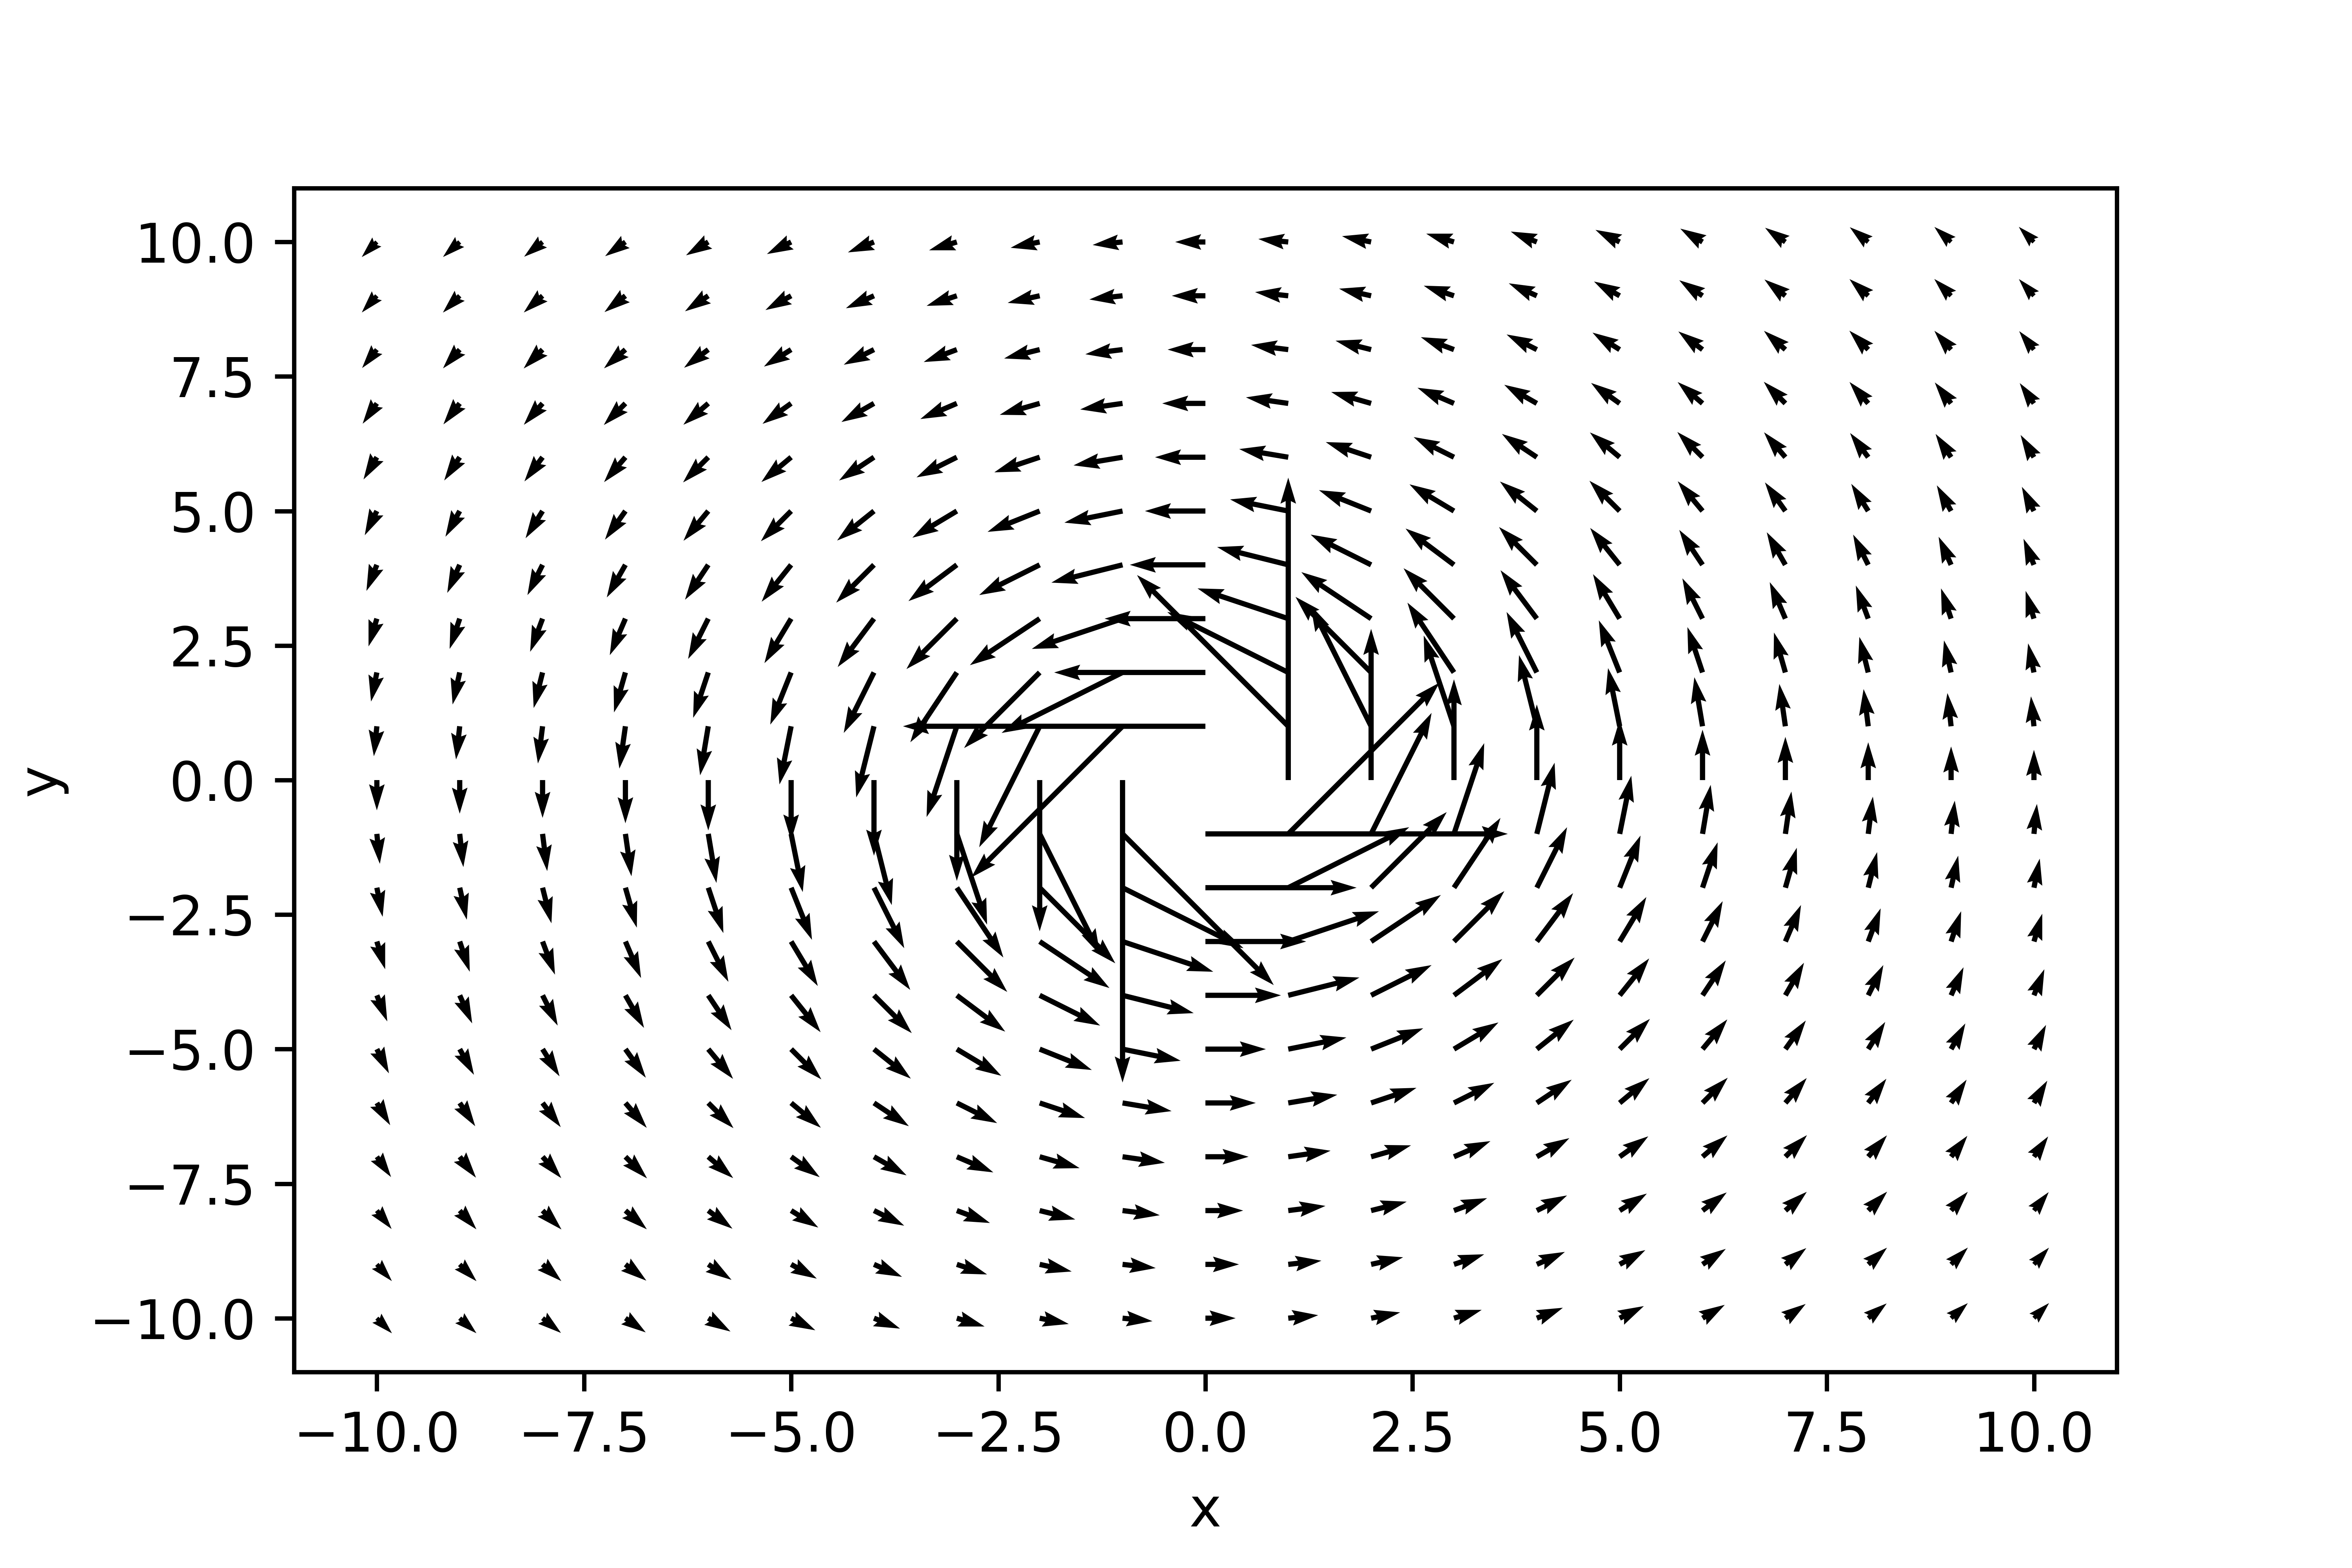
\includegraphics[width = .5\textwidth]{figs/vector_field_non_rot.png}
\caption{Die Vorticity dieses Vektorfeldes $\mathbf{v}$ ist gleich Null.}
\label{fig:nicht_rotierend}
\end{center}
\end{figure}
%
\begin{itemize}
\item Nehme das Feld $\mathbf{v} = \left(y, 0, 0\right)^T$. Die Stromlinien dieses Feldes sind nicht gekrümmt. Trotzdem gilt $\nabla\times\mathbf{v} = \left(0, 0, - 1\right)^T\not = \mathbf{0}$.
\item Nehme das Feld $\mathbf{v} = \frac{1}{x^2 + y^2}\left(-y, x, 0\right)^T$. Das Feld sieht sehr stark nach einem rotationsbehafteten Feld aus (s. Abb. \ref{fig:nicht_rotierend}). Trotzdem gilt

\begin{align}
\nabla\times\mathbf{v} & = \left(\frac{\partial}{\partial x}\frac{x}{x^2 + y^2} + \frac{\partial}{\partial y}\frac{y}{x^2 + y^2}
\right)\mathbf{e}_z\nonumber\\
& = \left(\frac{1}{x^2 + y^2} - x2x\frac{1}{\left(x^2 + y^2\right)^2} + \frac{1}{x^2 + y^2} - y2y\frac{1}{\left(x^2 + y^2\right)^2}\right)\mathbf{e}_z = \mathbf{0}.
\end{align}
%
\end{itemize}
%
Um die wahre Bedeutung der Vorticity zu verstehen, stellt man sich am besten ein 2D-Vektorfeld $\mathbf{v}_h = \left(u, v\right)^T$ vor (in kartesischen Koordinaten). Nehme ein Rechteck $\left[-a, a\right]\times\left[-b, b\right]$. $\mathbf{s}$ sei eine Kurve, die im positiven mathematischen Drehsinn diese Menge umschließt. Dann gilt näherungsweise mit $\left(u, v\right)$ als Vektor am Ursprung
%
\begin{align}
\int_{\mathbf{s}}^{}\mathbf{v}_h\cdot d\mathbf{s} &\approx 2a\left(u - b\frac{\partial u}{\partial y}\right) + 2b\left(v + a\frac{\partial v}{\partial x}\right) - 2a\left(u + b\frac{\partial u}{\partial y}\right) - 2b\left(v - a\frac{\partial v}{\partial x}\right)\nonumber\\
& = -2ba\frac{\partial u}{\partial y} + 2ba\frac{\partial v}{\partial x} - 2ab\frac{\partial u}{\partial y} + 2ba\frac{\partial v}{\partial x} = -4ba\frac{\partial u}{\partial y} + 4ab\frac{\partial v}{\partial x} = 4ab\left(\frac{\partial v}{\partial x} - \frac{\partial u}{\partial y}\right).
\end{align}
%
Der Flächeninhalt der Fläche ist $4ab$. Betrachtet man die Zirkulation des Vektorfelds um ein Teilchen, bildet also
%
\begin{align}
\lim\limits_{a, b\to 0}\frac{\int_{\mathbf{s}}^{}{\mathbf{v}_h\cdot d\mathbf{s}}}{4ab} = \frac{\partial v}{\partial x} - \frac{\partial u}{\partial y}, 
\end{align}
%
so ergibt sich die Definition der z-Komponente der Wirbelstärke. Die Komponenten der Rotation geben deshalb an, wie eine kleine Fläche in einer Ebene senkrecht zur jeweiligen Komponente umströmt wird. Es gibt also einen Zusammenhang von Zirkulation und Vorticity. In integraler Form ist dies die Aussage des \textit{Satzes von Stokes}\index{Stokes'scher Satz}\index{Satz von Stokes}:
%
\begin{align}
\int_{A}^{}\nabla\times\mathbf{v}\cdot d\mathbf{f} = \int_{\partial A}^{}\mathbf{v}\cdot d\mathbf{s}.\label{eq:satz_von_stokes}
\end{align}
%
Der Satz von Stokes verknüpft also genau wie die obige Betrachtung das vektorielle Kurvenintegral entlang des Randes einer Fläche mit der Wirbelstärke innerhalb der Fläche. Eine weitere Veranschaulichung der Vorticity wird im kommenden Abschnitt gezeigt.

\subsection{Scherungs- und Krümmungsvorticity}
\label{sec:scherungs_und_kruemmungsvorticity}\index{Scherungsvorticity}\index{Krümmungsvorticity}

Definiere o. B. d. A. in ebener Geometrie eine rechtshändige Orthonormalbasis $\mathbf{s}, \mathbf{n}, \mathbf{k}$, bei der $\mathbf{s}$ am Ursprung parallel zum Horizontalwind ist. Damit gilt
%
\begin{align}
\mathbf{v} = \left(\begin{array}{c}
V\cos\left(\beta\right)\\
V\sin\left(\beta\right)\\
w
\end{array}\right)\label{eq:wind_natuerlich}
\end{align}
%
mit der horizontalen Windgeschwindigkeit $V$ und dem Vertikalwind $w$. $\beta$ ist hier die horizontale Windrichtung relativ zu $\mathbf{s}$. Damit folgt für die Vorticity
%
\begin{align}
\zeta & = \frac{\partial}{\partial s}V\sin\left(\beta\right) - \frac{\partial}{\partial n}V\cos\left(\beta\right) = \sin\left(\beta\right)\frac{\partial V}{\partial s} + V\frac{\partial\beta}{\partial s}\cos\left(\beta\right) - \cos\left(\beta\right)\frac{\partial V}{\partial n} + V\sin\left(\beta\right)\frac{\partial \beta}{\partial n}.
\end{align}
%
Im Koordinatenursprung gilt $\beta = 0$, deshalb hat man dort
%
\begin{align}
\zeta = V\frac{\partial\beta}{\partial s} - \frac{\partial V}{\partial n}.
\end{align}
%
Den ersten Term $V\frac{\partial\beta}{\partial s}$ nennt man Krümmungsvorticity. Er ist größer Null, wenn die Stromlinie nach links gekrümmt ist, gleich Null, wenn die Stromlinie gerade ist, und bei einer nach rechts gekrümmten Stromlinie kleiner als Null. Den Term $-\frac{\partial V}{\partial n}$ nennt man Scherungsvorticity. Er ist größer Null, wenn die Windgeschwindigkeit rechts von der Windrichtung zunimmt. Insbesondere sieht man, dass ein Strömungsfeld mit gekrümmten Stromlinien rotationsfrei sein kann und eines mit geraden Stromlinien rotationsbehaftet.

\begin{figure}
\centering
\begin{subfigure}[c]{.4\textwidth}
\centering
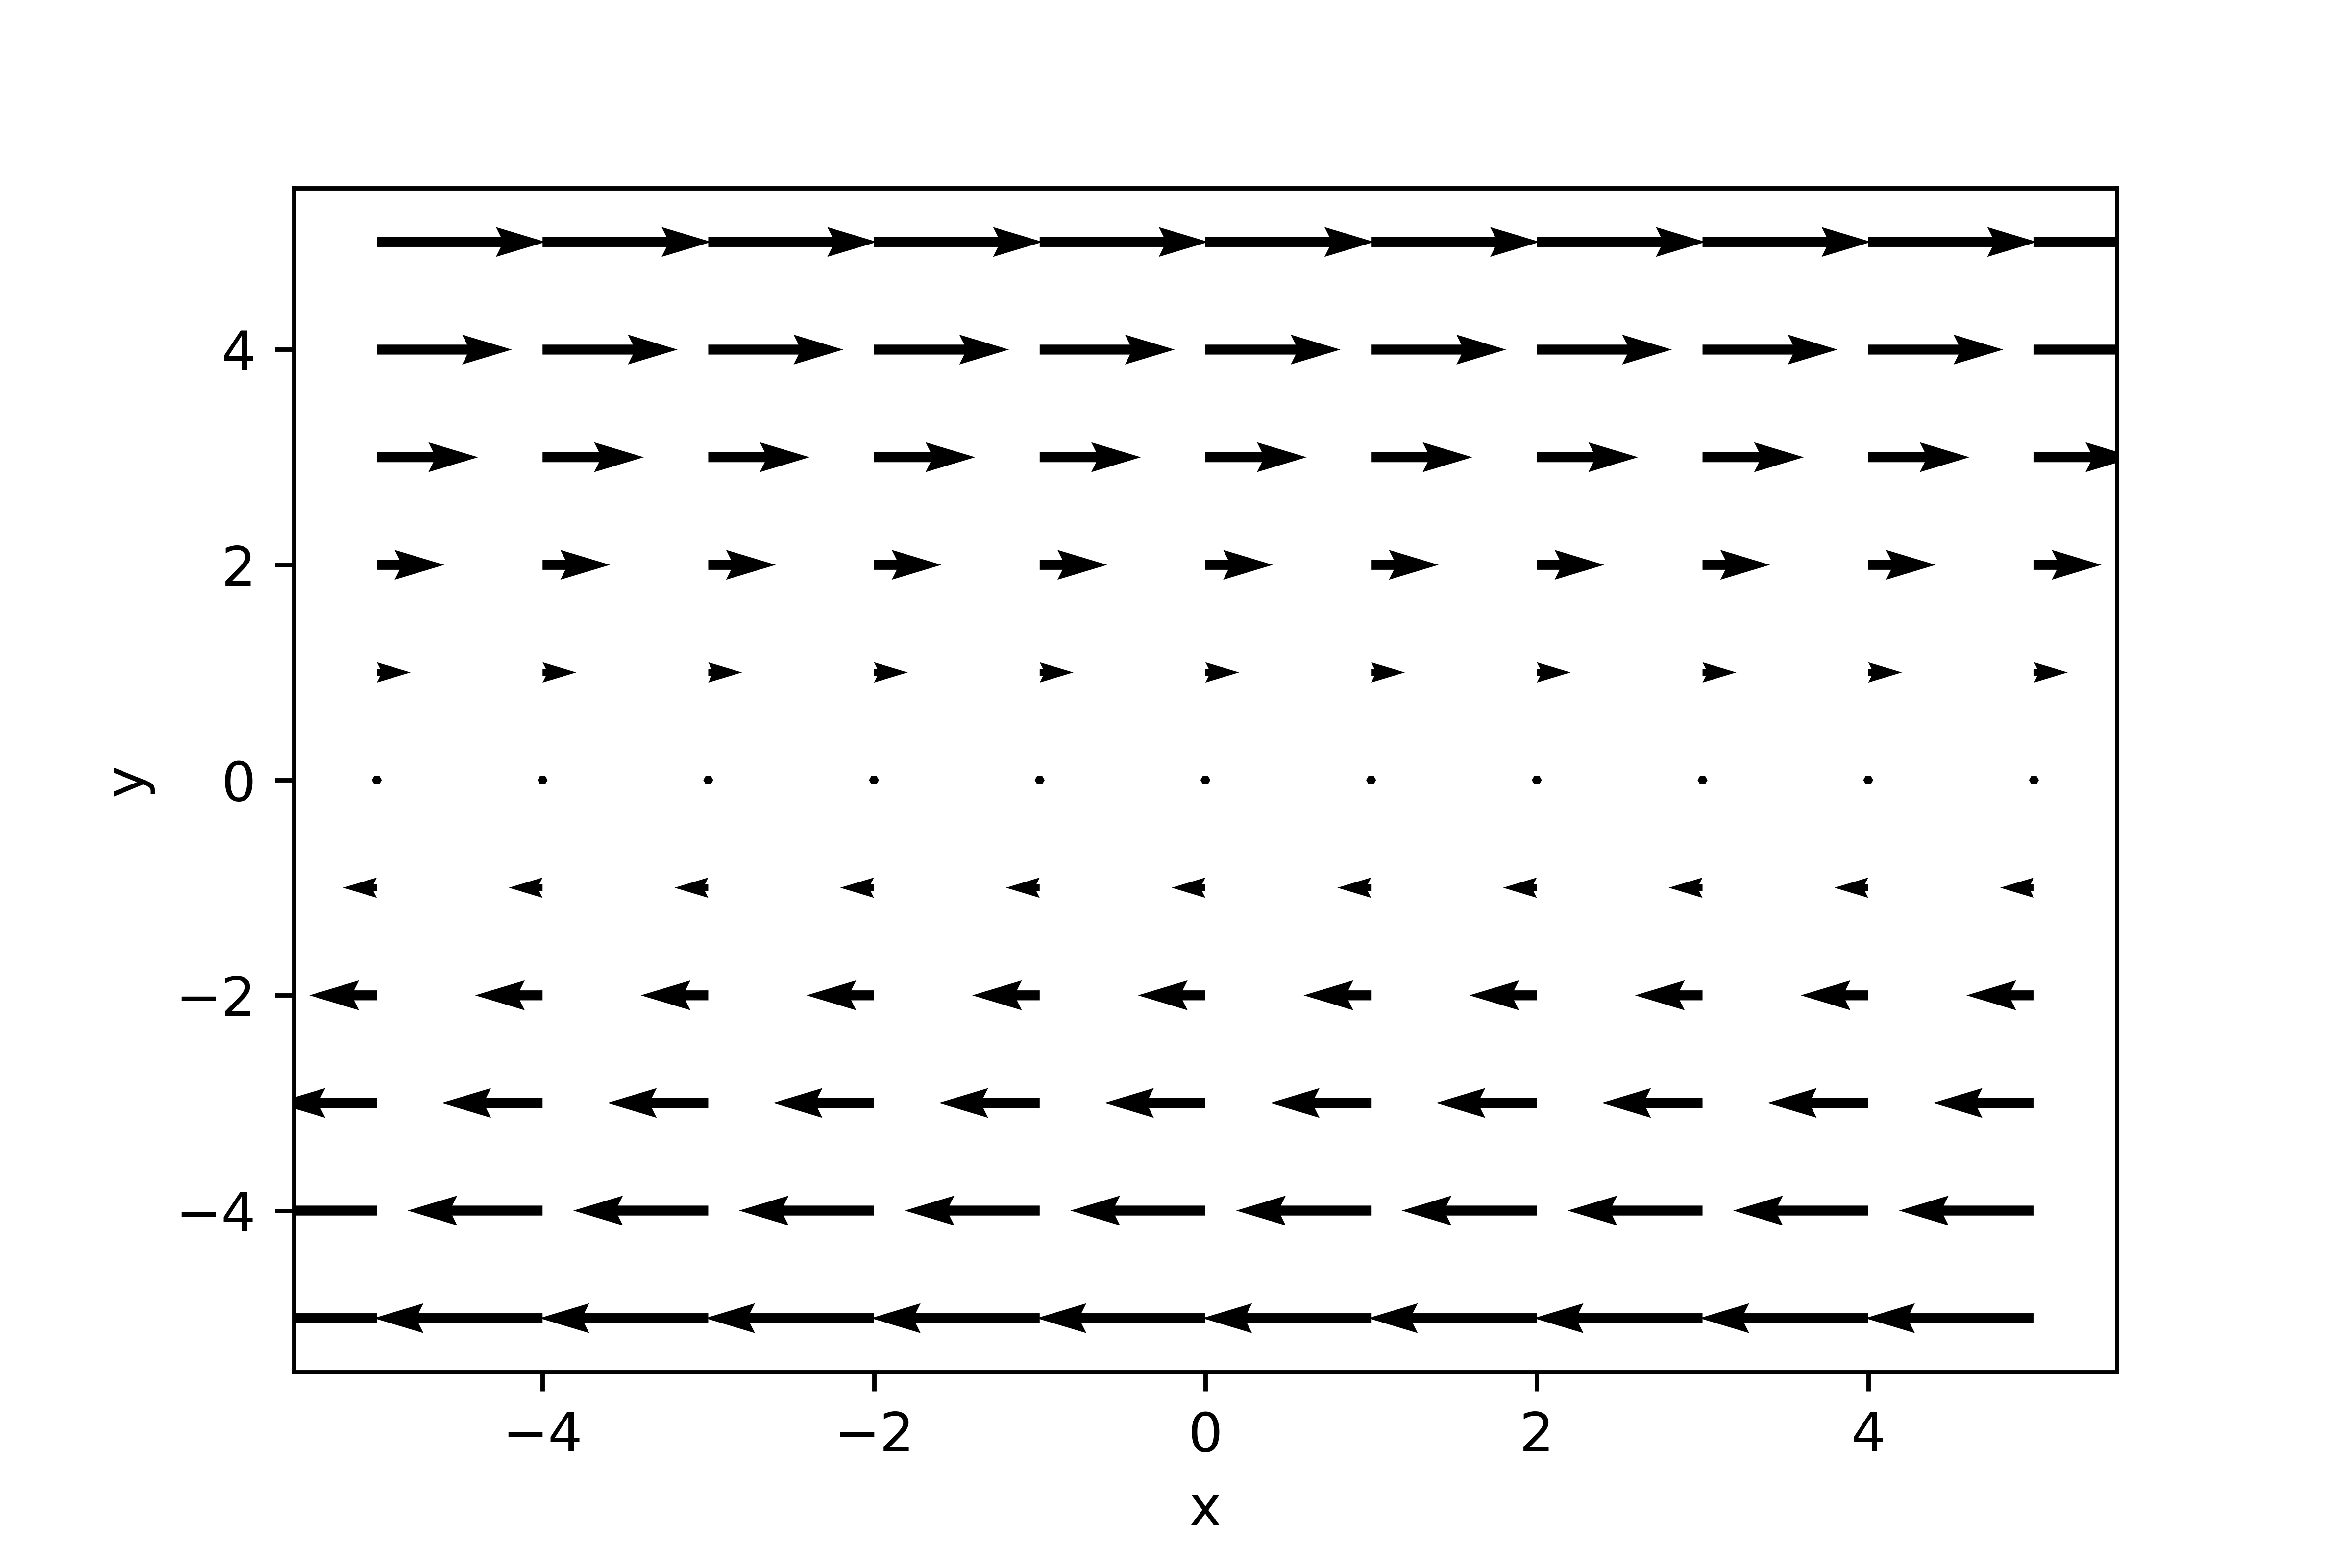
\includegraphics[height = 4cm]{figs/shear_vorticity.png}
\end{subfigure}
\begin{subfigure}[c]{.4\textwidth}
\centering
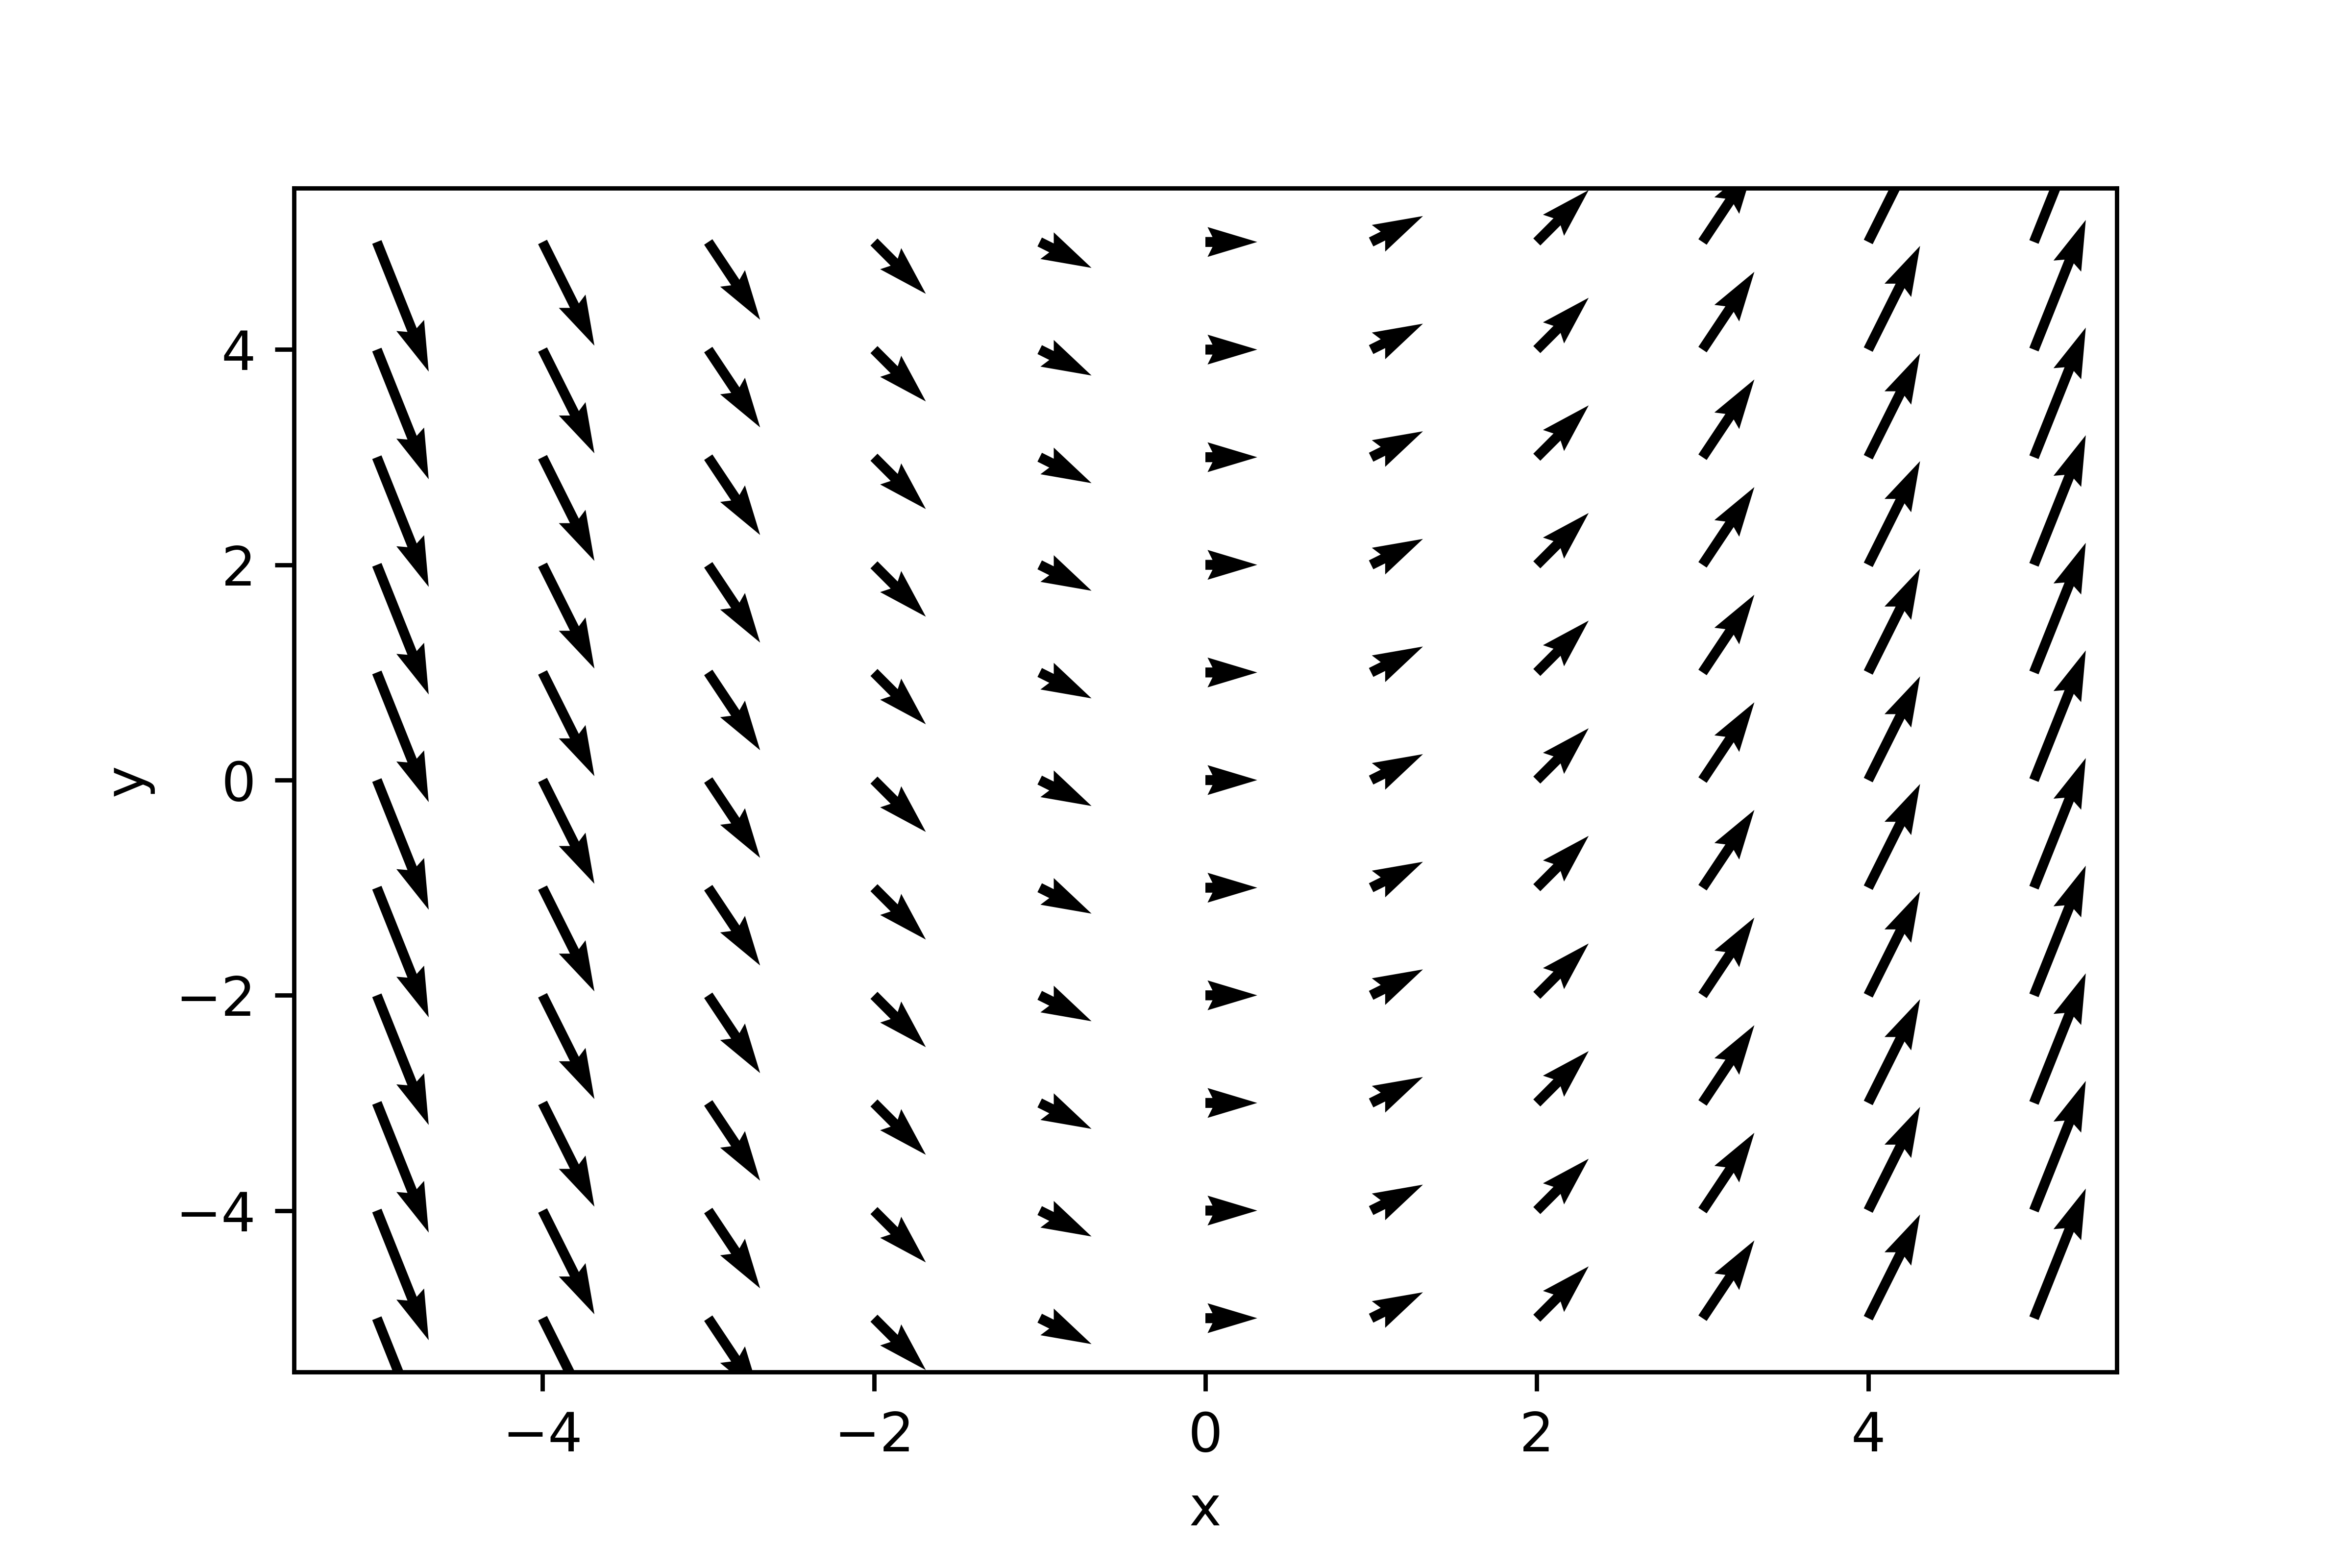
\includegraphics[height = 4cm]{figs/curvature_vorticity.png}
\end{subfigure}
\caption{Scherungsvorticity (links) und Krümmungsvorticity (rechts).}
\end{figure}

\subsection{Zirkulationssatz}
\label{sec:zirkulationssatz}\index{Zirkulationssatz}

Sei $A$ eine beliebig geformte Fläche im Raum, dann definiert man die Zirkulation $S$ des Windfeldes $\mathbf{v}$ um $A$ zur Zeit $t$ durch
%
\begin{align}
S\left(t\right) \coloneqq \int_{\partial A}\mathbf{v}\cdot d\mathbf{s} = \int_0^1\mathbf{v}\left(\mathbf{r}\left(\tau\right), t\right)\cdot\frac{d\mathbf{r}}{d\tau}d\tau,
\end{align}
%
wobei $\mathbf{r}\left(\tau\right)$ eine auf dem Intervall $\left[0, 1\right]$ definierte Funktion ist, die den Rand von $A$ durchläuft. Bewegt sich die Fläche $A$ mit dem Windfeld mit, so ändert sich auch die Zirkulation $S$ um $A$, also
%
\begin{align}
\md{S} = \md{}\int_0^1\mathbf{v}\left(\mathbf{r}\left(\tau\right), t\right)\cdot\frac{d\mathbf{r}}{d\tau}d\tau = \int_0^1\md{\mathbf{v}}\cdot\frac{d\mathbf{r}}{d\tau}d\tau + \int_0^1\mathbf{v}\cdot\md{}\left(\frac{d\mathbf{r}}{d\tau}\right)d\tau.
\end{align}
%
Um das zweite Integral näher zu bestimmen, stellt man vorbereitend
%
\begin{align}
\frac{d\mathbf{r}}{d\tau} & = \lim_{\Delta \to 0}\frac{\mathbf{r}\left(\tau + \Delta\right) - \mathbf{r}\left(\tau\right)}{\Delta}\nonumber\\
\Rightarrow \md{}\frac{d\mathbf{r}}{d\tau} & = \lim_{\Delta \to 0}\frac{\md{\mathbf{r}}\left(\tau + \Delta\right) - \md{\mathbf{r}}\left(\tau\right)}{\Delta} = \lim_{\Delta \to 0}\frac{\mathbf{v}\left(\mathbf{r}\left(\tau + \Delta\right)\right) - \mathbf{v}\left(\mathbf{r}\left(\tau\right)\right)}{\Delta}\nonumber\\
& = \left(\frac{d\mathbf{r}}{d\tau}\cdot\nabla\right)\mathbf{v}
\end{align}
%
fest. Definiere $\mathbf{v}\left(\tau\right) \coloneqq \mathbf{v}\left(\mathbf{r}\left(\tau\right), t\right)$, dann gilt
%
\begin{align}
\left(\frac{d\mathbf{r}}{d\tau}\cdot\nabla\right)\mathbf{v} = \frac{d\mathbf{v}}{d\tau},
\end{align}
%
womit man
%
\begin{align}
\int_0^1\mathbf{v}\cdot\md{}\left(\frac{d\mathbf{r}}{d\tau}\right)d\tau = \int_0^1\mathbf{v}\cdot\frac{d\mathbf{v}}{d\tau}d\tau  = \frac{1}{2}\left[\mathbf{v}^2\right]_0^1 = 0
\end{align}
%
erhält, da aufgrund der Geschlossenheit der Kurve $\mathbf{v}\left(0\right) = \mathbf{v}\left(1\right)$ gilt. Mit dem Stokes'schen Satz folgt
%
\begin{align}
\md{S} = \int_A\nabla\times\mathbf{F}\cdot d\mathbf{n},
\end{align}
%
wobei $\mathbf{F}$ die Summe aller wirkenden Kräfte ist. Konservative Kräfte ändern die Zirkulation also nicht. Mit
%
\begin{align}
\nabla\times\left(-\frac{1}{\rho}\nabla p\right) & \stackrel{\text{Glg. \eqref{eq:diff_op_rule_5}}}{=} \frac{1}{\rho^2}\nabla\rho\times\nabla p,\\
\nabla\times\mathbf{v}\times\mathbf{f} & \stackrel{\text{Glg. \eqref{eq:diff_op_rule_7}}}{=} \left(\mathbf{f}\cdot\nabla\right)\mathbf{v} - \mathbf{f}\nabla\cdot\mathbf{v}
\end{align}
%
folgt
%
\begin{center}
\doublebox{\parbox{\textwidth}{
\begin{center}
\begin{align}
\md{S} = \int_A\left(\frac{1}{\rho^2}\nabla\rho\times\nabla p + \left(\mathbf{f}\cdot\nabla\right)\mathbf{v} - \mathbf{f}\nabla\cdot\mathbf{v} + \nabla\times\mathbf{f}_R\right)\cdot d\mathbf{n}.\label{eq:circ_theorem}
\end{align}
\end{center}
}}
\end{center}
%
In IS gilt also in barotropen idealen Medien
%
\begin{align}
\md{S} = 0 \Leftrightarrow S = \text{const.}\label{eq:circ_theorem_mod_1}
\end{align}

\subsection{Vorticitygleichung}
\label{sec:vorticitygleichung}\index{Vorticitygleichung}

Die Impulsgleichung Glg. \eqref{eq:momentum_mod} lautet
%
\begin{align}
\frac{\partial\mathbf{v}}{\partial t} & = -\frac{1}{\rho}\nabla p + \mathbf{v}\times\etabi - \nabla k + \mathbf{g} + \mathbf{f}_R.
\end{align}
%
Nun wendet man auf die einzelnen Terme den Operator $\nabla\times $ an:
%
\begin{align}
\nabla\times\frac{\partial\mathbf{v}}{\partial t}&\stackrel{\text{Glg. \eqref{eq:diff_op_rule_4}}}{=} \frac{\partial}{\partial t}\nabla\times\mathbf{v}\\
\nabla\times\left(-\frac{1}{\rho}\nabla p\right)&\stackrel{\text{Glg. \eqref{eq:diff_op_rule_5}}}{=} -\frac{1}{\rho^2}\nabla p\times\nabla\rho\\
\nabla\times\left(\mathbf{v}\times\etabi\right)&\stackrel{\text{Glg. \eqref{eq:diff_op_rule_7}}}{=} -\left(\mathbf{v}\cdot\nabla\right)\etabi - \etabi\nabla\cdot\mathbf{v} + \left(\etabi\cdot\nabla\right)\mathbf{v}\\
\nabla\times\mathbf{g}&\stackrel{\text{Glg. \eqref{eq:diff_op_rule_1}}}{=} \mathbf{0}\\
\nabla\times\nabla k&\stackrel{\text{Glg. \eqref{eq:diff_op_rule_1}}}{=} \mathbf{0}.
\end{align}
%
Somit gilt
%
\begin{align}
\frac{\partial}{\partial t}\text{rot}\left(\mathbf{v}\right) & = \frac{1}{\rho^2}\nabla\rho\times\nabla p - \left(\mathbf{v}\cdot\nabla\right)\etabi - \etabi\nabla\cdot\mathbf{v} + \left(\etabi\cdot\nabla\right)\mathbf{v} + \nabla\times\mathbf{f}_R.\label{eq:vorticity_eq_3d}
\end{align}
%
Durch Projektion auf die lokale Senkrechte erhält man
%
\begin{align}
\frac{\partial\zeta}{\partial t} & = \frac{1}{\rho^2}\mathbf{k}\cdot\left(\nabla\rho\times\nabla p\right) - \eta\nabla\cdot\mathbf{v}\nonumber\\
&  + \mathbf{k}\cdot\left[\left(\etabi\cdot\nabla\right)\mathbf{v}\right] - \mathbf{k}\cdot\left[\left(\mathbf{v}\cdot\nabla\right)\etabi\right] + \mathbf{k}\cdot\nabla\times\mathbf{f}_R.
\end{align}
%
Man rechnet zunächst mit Glg. \eqref{eq:diff_op_rule_11}
%
\begin{align}
\left(\etabi\cdot\nabla\right)w = \left(\etabi\cdot\nabla\right)\left(\mathbf{v}\cdot\mathbf{k}\right) & = \mathbf{k}\cdot\left[\left(\etabi\cdot\nabla\right)\mathbf{v}\right] + \mathbf{v}\cdot\left[\left(\etabi\cdot\nabla\right)\mathbf{k}\right]\nonumber\\
\Rightarrow\mathbf{k}\cdot\left[\left(\etabi\cdot\nabla\right)\mathbf{v}\right] & = \left(\etabi\cdot\nabla\right)w - \mathbf{v}\cdot\left[\left(\etabi\cdot\nabla\right)\mathbf{k}\right],\\
\mathbf{v}\cdot\nabla\eta = \left(\mathbf{v}\cdot\nabla\right)\left(\etabi\cdot\mathbf{k}\right) & = \etabi\cdot\left[\left(\mathbf{v}\cdot\nabla\right)\mathbf{k}\right] + \mathbf{k}\cdot\left[\left(\mathbf{v}\cdot\nabla\right)\etabi\right]\nonumber\\
\Rightarrow\mathbf{k}\cdot\left[\left(\mathbf{v}\cdot\nabla\right)\etabi\right] & = \mathbf{v}\cdot\nabla\eta - \etabi\cdot\left[\left(\mathbf{v}\cdot\nabla\right)\mathbf{k}\right].
\end{align}
%
Somit gilt
%
\begin{align}
\frac{\partial\zeta}{\partial t} & = \frac{1}{\rho ^2}\mathbf{k}\cdot\left(\nabla\rho\times\nabla p\right) - \eta\nabla\cdot\mathbf{v} + \left(\etabi\cdot\nabla\right)w - \mathbf{v}\cdot\left[\left(\etabi\cdot\nabla\right)\mathbf{k}\right] - \mathbf{v}\cdot\nabla\eta\nonumber\\
&  + \etabi\cdot\left[\left(\mathbf{v}\cdot\nabla\right)\mathbf{k}\right] + \mathbf{k}\cdot\nabla\times\mathbf{f}_R.
\end{align}
%
Es gelten mit den Feststellungen in Absch. \ref{sec:kugelkoordinaten}
%
\begin{align}
\frac{\partial\mathbf{k}}{\partial x} = \frac{\mathbf{i}}{r}, && \frac{\partial\mathbf{k}}{\partial y} = \frac{\mathbf{j}}{r}, && \frac{\partial\mathbf{k}}{\partial z} = \mathbf{0}.
\end{align}
%
Somit folgt
%
\begin{align}
\frac{\partial\zeta}{\partial t} & = \frac{1}{\rho ^2}\mathbf{k}\cdot\left(\nabla\rho\times\nabla p\right) - \eta\nabla\cdot\mathbf{v} + \etabi\cdot\nabla w - \frac{u\eta_x}{r} - \frac{v\eta_y}{r} - \mathbf{v}\cdot\nabla\eta + \frac{\eta_xu}{r} + \frac{\eta_yv}{r} + \mathbf{k}\cdot\nabla\times\mathbf{f}_R.
\end{align}
%
Die Vorticitygleichung lautet schlussendlich
%
\begin{center}
\doublebox{\parbox{\textwidth}{
\begin{center}
\begin{align}
\frac{\partial\zeta}{\partial t} = -\mathbf{v}\cdot\nabla\eta - \eta\nabla\cdot\mathbf{v} + \etabi\cdot\nabla w + \frac{1}{\rho ^2}\mathbf{k}\cdot\left(\nabla\rho\times\nabla p\right) + \mathbf{k}\cdot\nabla\times\mathbf{f}_R\label{eq:vorticit_z}.
\end{align}
\end{center}
}}
\end{center}
%
Geht man von einem Flachgeofluid aus, vernachlässigt die Reibung und führt einen horizontalen Windvektor $\mathbf{v}_h$ ein, folgt
%
\begin{align}
\frac{\partial\zeta}{\partial t} = -\mathbf{v}_h\cdot\nabla\eta - w\frac{\partial\zeta}{\partial z} - \eta\nabla\cdot\mathbf{v} + \etabi\cdot\nabla w + \frac{1}{\rho ^2}\mathbf{k}\cdot\left(\nabla\rho\times\nabla p\right).
\end{align}
%
Im barotropen Fall fällt hier der sogenannte \textit{Solenoidterm}\index{Solenoidterm}, der $\nabla\rho\times\nabla p$ enthält, weg, vernachlässigt man außerdem die vertikale Scherung des Horizontalwindes (s. Absch. \ref{sec:barotropie}), folgt
%
\begin{center}
\doublebox{\parbox{\textwidth}{
\begin{center}
\begin{align}
\frac{\partial\zeta}{\partial t} = -\mathbf{v}_h\cdot\nabla\eta - \eta\nabla\cdot\mathbf{v} + \etabi\cdot\nabla w.\label{eq:vorticit_z_baro}
\end{align}
\end{center}
}}
\end{center}
%
Dies ist die sogenannte \textit{barotrope Vorticitygleichung}\index{barotrope Vorticitygleichung}\index{Vorticitygleichung!barotrope}. Im Fall von Inkompressibilität, insbesondere im Fall der SWEs, ist $\nabla\cdot\mathbf{v} = 0$, woraus folgt
%
\begin{align}
\frac{\partial\zeta}{\partial t} = -\mathbf{v}_h\cdot\nabla\eta + \etabi\cdot\nabla w\Rightarrow\frac{d\eta}{dt} = \etabi\cdot\nabla w.
\end{align}
%
Vernachlässigt man die horizontalen Gradienten von $w$, folgt
%
\begin{align}
\frac{d\eta}{dt} = \eta\frac{\partial w}{\partial z}.\label{eq:vorticit_z_baro_swes_pre}
\end{align}
%
Setzt man
%
\begin{align}
\nabla\cdot\mathbf{v} & = \nabla\cdot\mathbf{v}_h + \frac{\partial w}{\partial z} = 0
\end{align}
%
ein, wobei ein breitenunabhängiger Krümmungsterm $\propto\frac{w}{r}$ vernachlässigt wurde, folgt
%
\begin{align}
\frac{d\eta}{dt} = -\eta\nabla\cdot\mathbf{v}_h.\label{eq:vorticit_z_baro_swes}
\end{align}
%
Im inkompressiblen, horizontaldivergenzfreien, barotropen Fall (außerdem wurde die vertikale Scherung des Horizontalwindes unterschlagen) ist die absolute Vorticity also eine Erhaltungsgröße.

\subsubsection{Vorticitygleichung im p-System}
\label{sec:vorticitygleichung_psystem}\index{Vorticitygleichung!p-System}

Nun soll dasselbe im p-System durchgeführt werden. Die Impulsgleichungen Glg.en \eqref{eq:x_momentum_simplified_simplified_p} - \eqref{eq:y_momentum_simplified_simplified_p} im p-System lauten vektoriell
%
\begin{align}
\frac{\partial\mathbf{v}_h}{\partial t} & = -\nabla\phi - \frac{1}{2}\nabla\left(\mathbf{v}_h\cdot\mathbf{v}_h\right) + \mathbf{v}_h\times\etabi' - \omega\frac{\partial\mathbf{v}_h}{\partial p} + \nabla\times\mathbf{f}_R^{(H)}.
\end{align}
%
Dabei wurde die modifizierte absolute Vorticity $\etabi'$ durch
%
\begin{align}
\etabi' \coloneqq f\mathbf{k} + \nabla\times\mathbf{v}_h
\end{align}
%
definiert. Nun wendet man auf die einzelnen Terme den Operator $\nabla\times $ an:
%
\begin{align}
\nabla\times\frac{\partial\mathbf{v}_h}{\partial t}&\stackrel{\text{Glg. \eqref{eq:diff_op_rule_4}}}{=} \frac{\partial}{\partial t}\nabla\times\mathbf{v}_h\\
\nabla\times\nabla\phi&\stackrel{\text{Glg. \eqref{eq:diff_op_rule_1}}}{=} \mathbf{0}\\
\nabla\times\mathbf{g}&\stackrel{\text{Glg. \eqref{eq:diff_op_rule_1}}}{=} \mathbf{0}\\
\nabla\times\nabla\left(\mathbf{v}_h\cdot\mathbf{v}_h\right)&\stackrel{\text{Glg. \eqref{eq:diff_op_rule_1}}}{=} \mathbf{0}\\
\nabla\times\left(\mathbf{v}_h\times\etabi'\right)&\stackrel{\text{Glg. \eqref{eq:diff_op_rule_7}}}{=} -\left(\mathbf{v}_h\cdot\nabla\right)\etabi' - \etabi'\nabla\cdot\mathbf{v}_h + \left(\etabi'\cdot\nabla\right)\mathbf{v}_h\\
\nabla\times\left(\omega\frac{\partial\mathbf{v}_h}{\partial p}\right)&\stackrel{\text{Glg. \eqref{eq:diff_op_rule_5}}}{=} \omega\nabla\times\frac{\partial\mathbf{v}_h}{\partial p} - \frac{\partial\mathbf{v}_h}{\partial p}\times\nabla\omega
\end{align}
%
Somit gilt
%
\begin{align}
\frac{\partial}{\partial t}\nabla\times\mathbf{v}_h & = -\left(\mathbf{v}_h\cdot\nabla\right)\etabi' - \etabi'\nabla\cdot\mathbf{v}_h + \left(\etabi'\cdot\nabla\right)\mathbf{v}_h + \omega\nabla\times\frac{\partial\mathbf{v}_h}{\partial p} - \frac{\partial\mathbf{v}_h}{\partial p}\times\nabla\omega + \nabla\times\mathbf{f}_R^{(H)}.
\end{align}
%
Durch Projektion auf die lokale Senkrechte $\mathbf{k}$ erhält man
%
\begin{align}
\frac{\partial\zeta}{\partial t} & = -\mathbf{k}\cdot\left[\left(\mathbf{v}_h\cdot\nabla\right)\etabi'\right] - \left(f + \zeta\right)\nabla\cdot\mathbf{v}_h + \mathbf{k}\cdot\left[\left(\etabi'\cdot\nabla\right)\mathbf{v}_h\right]\nonumber\\
&  - \omega\frac{\partial\zeta}{\partial p} + \mathbf{k}\cdot\left[\frac{\partial\mathbf{v}_h}{\partial p}\times\nabla\omega\right] + \mathbf{k}\cdot\nabla\times\mathbf{f}_R^{(H)}.
\end{align}
%
Man rechnet zunächst mit Glg. \eqref{eq:diff_op_rule_11}
%
\begin{align}
0 = \left(\etabi'\cdot\nabla\right)\left(\mathbf{v}_h\cdot\mathbf{k}\right) & = \mathbf{k}\cdot\left[\left(\etabi'\cdot\nabla\right)\mathbf{v}_h\right] + \mathbf{v}_h\cdot\left[\left(\etabi'\cdot\nabla\right)\mathbf{k}\right]\nonumber\\
\Rightarrow\mathbf{k}\cdot\left[\left(\etabi'\cdot\nabla\right)\mathbf{v}_h\right] & = -\mathbf{v}_h\cdot\left[\left(\etabi'\cdot\nabla\right)\mathbf{k}\right],\\
\mathbf{v}_h\cdot\nabla\eta = \left(\mathbf{v}_h\cdot\nabla\right)\left(\etabi'\cdot\mathbf{k}\right) & = \etabi'\cdot\left[\left(\mathbf{v}_h\cdot\nabla\right)\mathbf{k}\right] + \mathbf{k}\cdot\left[\left(\mathbf{v}_h\cdot\nabla\right)\etabi'\right]\nonumber\\
\Rightarrow\mathbf{k}\cdot\left[\left(\mathbf{v}_h\cdot\nabla\right)\etabi'\right] & = \mathbf{v}_h\cdot\nabla\eta - \etabi'\cdot\left[\left(\mathbf{v}_h\cdot\nabla\right)\mathbf{k}\right].
\end{align}
%
Es gelten mit den Feststellungen in Absch. \ref{sec:kugelkoordinaten}
%
\begin{align}
\frac{\partial\mathbf{k}}{\partial x} = \frac{\mathbf{i}}{r}, && \frac{\partial\mathbf{k}}{\partial y} = \frac{\mathbf{j}}{r}, && \frac{\partial\mathbf{k}}{\partial z} = \mathbf{0}.
\end{align}
%
Somit folgt
%
\begin{align}
\mathbf{v}_h\cdot\left[\left(\etabi'\cdot\nabla\right)\mathbf{k}\right] & = \etabi'\cdot\left[\left(\mathbf{v}_h\cdot\nabla\right)\mathbf{k}\right].
\end{align}
%
Die Vorticitygleichung im p-System lautet somit
%
\begin{center}
\doublebox{\parbox{\textwidth}{
\begin{center}
\begin{align}
\frac{\partial\zeta}{\partial t} & = -v\beta - \left(f + \zeta\right)\nabla\cdot\mathbf{v}_h - \mathbf{v}_h\cdot\nabla\zeta - \omega\frac{\partial\zeta}{\partial p} + \mathbf{k}\cdot\left[\frac{\partial\mathbf{v}_h}{\partial p}\times\nabla\omega\right] + \mathbf{k}\cdot\nabla\times\mathbf{f}_R^{(H)}.\label{eq:vorticity_p}
\end{align}
\end{center}
}}
\end{center}
%
Berechnet man die Vorticity des geostrophischen Windfeldes erhält man
%
\begin{align}
\zeta_g = \frac{1}{f}\frac{\partial^2\phi}{\partial x^2} + \frac{1}{f}\frac{\partial^2\phi}{\partial y^2} - \frac{\beta}{f^2}\frac{\partial\phi}{\partial y} + \frac{\tan\left(\varphi\right)u}{r} = \frac{1}{f}\Delta_h\phi + \frac{\beta}{f}u + \frac{\tan\left(\varphi\right)u}{r}.\label{eq:geostro_vort_skal}
\end{align}
%
Für den ersten Term gilt
%
\begin{align}
\mathcal{O}\left(\frac{1}{f}\Delta\phi\right) = \mathcal{O}\left(\frac{1}{f}\frac{\Delta p}{\rho L^2}\right) = 10^{-5}\:\frac{1}{\text{s}}.
\end{align}
%
Der Term des $\beta-$Effekts hat in mittleren Breiten eine Größenordnung von $10^{-6}$ 1/s. Daher kann man in den Extratropen die Vorticity durch die geostrophische Vorticity nähern und den Term des $\beta-$Effektes vernachlässigen.

\subsection{Barotrope potentielle Vorticity}
\label{sec:barotrope_potentielle_vorticity}\index{Vorticity!potentielle!barotrope}\index{barotrope potentielle Vorticity}

In der Dynamik der SWEs ist die \textit{barotrope potentielle Vorticity} (barotrope PV) $q$ definiert durch
%
\begin{align}
q \coloneqq\frac{\eta}{h} = \frac{\zeta + f}{h} = \frac{\mathbf{k}\cdot\left(\nabla\times\mathbf{v}\right) + f}{h}, 
\end{align}
%
hierbei ist $h$ die Tiefe. Nach Glg. \eqref{eq:diff_op_rule_10} gilt
%
\begin{align}
\left(\mathbf{v}\cdot\nabla\right)\mathbf{v} & = \nabla k - \mathbf{v}\times\left(\nabla\times\mathbf{v}\right)
\end{align}
%
mit der spezifischen kinetischen Energie $k = \frac{1}{2}\mathbf{v}^2$. Für den zweiten Term gilt mit Glg. \eqref{eq:rot_shallow}
%
\begin{align}
\mathbf{v}\times\left(\nabla\times\mathbf{v}\right) & = \mathbf{v}\times\left[\frac{u\tan\left(\varphi\right)}{r}\mathbf{k} + \mathbf{k}\left(\frac{\partial v}{\partial x} - \frac{\partial u}{\partial y}\right) + \mathbf{j}\frac{\partial u}{\partial z} - \mathbf{i}\frac{\partial v}{\partial z}\right].
\end{align}
%
Aufgrund des Verschwindens vertikaler Scherung im barotropen Fall gilt
%
\begin{align}
\mathbf{v}\times\left(\nabla\times\mathbf{v}\right) & = \mathbf{v}\times\left[\frac{u\tan\left(\varphi\right)}{r}\mathbf{k} + \mathbf{k}\left(\frac{\partial v}{\partial x} - \frac{\partial u}{\partial y}\right)\right] = \mathbf{v}\times\mathbf{k}\left(\frac{\partial v}{\partial x} - \frac{\partial u}{\partial y} + \frac{u\tan\left(\varphi\right)}{r}\right) = \mathbf{v}\times\mathbf{k}\zeta = -\mathbf{k}\times\zeta\mathbf{v}.
\end{align}
%
Die Vertikalkomponente interessiert hier nicht weiter. Nun kann man für die Impulsgleichung der Flachwassergleichungen Glg. \eqref{eq:swe_0} unter Vernachlässigung der Reibung schreiben
%
\begin{align}
\frac{\partial\mathbf{v}}{\partial t} + \mathbf{k}\times\zeta\mathbf{v} & = -g\nabla\left(h + b\right) - \nabla k - f\mathbf{k}\times\mathbf{v}\nonumber\\
\Leftrightarrow\frac{\partial\mathbf{v}}{\partial t} + qh\mathbf{k}\times\mathbf{v} & = -g\nabla\left(h + b\right) - \nabla k.
\end{align}
%
Es gilt
%
\begin{center}
\doublebox{\parbox{0.8\textwidth}{
\begin{center}
\begin{align}
\md{q} & = \frac{1}{h}\md{\eta} - \frac{\eta}{h^2}\md{h}\stackrel{\text{Glg. \eqref{eq:swe_1}}}{=} - \frac{\eta}{h}\nabla\cdot\mathbf{v} - \frac{\eta}{h^2}\left(-h\nabla\cdot\mathbf{v}\right) = 0.\label{eq:pv_conservation_baro}
\end{align}
\end{center}
}}
\end{center}
%
Die barotrope PV ist also eine Erhaltungsgröße. In den mittleren Breiten ist die planetare Vorticity eine Größenordnung größer als die relative, somit folgt aus der Tatsache, dass die barotrope potentielle Vorticity erhalten ist
%
\begin{align}
h\downarrow \Rightarrow \left(\zeta + f\right)\downarrow \Rightarrow \zeta\downarrow, 
\end{align}
%
wobei von einem postiven Vorzeichen von $f$ und somit auch von $\eta$ ausgegangen wurde. Bei negativem $f$ gilt analog, dass $\zeta$ wachsen muss. Trifft eine Westströmung also auf ein orographisches Hindernis, so entsteht antizyklonale relative Vorticity. Dies bezeichnet man als \textit{orographischen $\beta-$Effekt}\index{$\beta-$Effekt!orographischer}\index{orographischer $\beta-$Effekt}. Ein wichtiges Beispiel ist das Entstehen planetarer Wellen an den Rocky Mountains.

Glg. \eqref{eq:pv_conservation_baro} kann man in der Form
%
\begin{align}
\frac{\partial q}{\partial t} + \mathbf{v}\cdot\nabla h = 0
\end{align}
%
notieren. Kombiniert man dies mit Glg. \eqref{eq:swe_1}, erhält man
%
\begin{align}
h\frac{\partial q}{\partial t} + h\mathbf{v}\cdot\nabla q + q\frac{\partial h}{\partial t} + qh\nabla\cdot\mathbf{v} + q\mathbf{v}\cdot\nabla h = 0\nonumber
\end{align}
\begin{center}
\doublebox{\parbox{0.8\textwidth}{
\begin{center}
\begin{align}
\Leftrightarrow \frac{\partial\left(hq\right)}{\partial t} + \nabla\cdot\left(hq\mathbf{v}\right) = 0.\label{eq:pv_conservation_baro_flux}
\end{align}
\end{center}
}}
\end{center}

\subsection{Helizität}
\label{sec:helizität}\index{Helizität}

Man definiert die \textit{Helizität}\index{Helizität} $Z$ durch
%
\begin{align}
Z \coloneqq \mathbf{v}\cdot\zetabi.\label{eq:def_helicity}
\end{align}
%
Die Impulsgleichung Glg. \eqref{eq:momentum_mod} lautet
%
\begin{align}
\frac{\partial\mathbf{v}}{\partial t} & = -\frac{1}{\rho}\nabla p + \mathbf{v}\times\mathbf{f} + \mathbf{v}\times\zetabi - \nabla k + \mathbf{g} + \mathbf{f}_R.
\end{align}
%
Projiziert man dies auf $\zetabi$, erhält man
%
\begin{align}
\zetabi\cdot\frac{\partial\mathbf{v}}{\partial t} & = -\frac{\zetabi}{\rho}\cdot\nabla p + \zetabi\cdot\left(\mathbf{v}\times\mathbf{f}\right) - \zetabi\cdot\nabla k + \zetabi\cdot\mathbf{g} + \zetabi\cdot\mathbf{f}_R.
\end{align}
%
Die dreidimensionale Vorticitygleichung Glg. \eqref{eq:vorticity_eq_3d} lautet
%
\begin{align}
\frac{\partial\zetabi}{\partial t} & = \frac{1}{\rho^2}\nabla\rho\times\nabla p - \left(\mathbf{v}\cdot\nabla\right)\zetabi - \mathbf{f}\nabla\cdot\mathbf{v} - \zetabi\nabla\cdot\mathbf{v} + \left(\mathbf{f}\cdot\nabla\right)\mathbf{v} + \left(\zetabi\cdot\nabla\right)\mathbf{v} + \nabla\times\mathbf{f}_R.
\end{align}
%
Projiziert man dies auf $\mathbf{v}$, erhält man
%
\begin{align}
\mathbf{v}\cdot\frac{\partial\zetabi}{\partial t} &= \frac{\mathbf{v}}{\rho^2}\cdot\left(\nabla\rho\times\nabla p\right) - \mathbf{v}\cdot\left[\left(\mathbf{v}\cdot\nabla\right)\zetabi\right] - \mathbf{v}\cdot\mathbf{f}\nabla\cdot\mathbf{v} - \mathbf{v}\cdot\zetabi\nabla\cdot\mathbf{v} + \mathbf{f}\cdot\nabla k + \zetabi\cdot\nabla k + \mathbf{v}\cdot\left(\nabla\times\mathbf{f}_R\right)\nonumber\\
\Leftrightarrow\mathbf{v}\cdot\frac{\partial\zetabi}{\partial t} &= \frac{\mathbf{v}}{\rho^2}\cdot\left(\nabla\rho\times\nabla p\right) - \left(\mathbf{v}\cdot\nabla\right)\left(\mathbf{v}\cdot\zetabi\right) + \zetabi\cdot\left[\left(\mathbf{v}\cdot\nabla\right)\mathbf{v}\right] - \mathbf{v}\cdot\mathbf{f}\nabla\cdot\mathbf{v} - \mathbf{v}\cdot\zetabi\nabla\cdot\mathbf{v} + \mathbf{f}\cdot\nabla k + \zetabi\cdot\nabla k + \mathbf{v}\cdot\left(\nabla\times\mathbf{f}_R\right)\nonumber\\
\Leftrightarrow\mathbf{v}\cdot\frac{\partial\zetabi}{\partial t} &= \frac{\mathbf{v}}{\rho^2}\cdot\left(\nabla\rho\times\nabla p\right) - \left(\mathbf{v}\cdot\nabla\right)\left(\mathbf{v}\cdot\zetabi\right) + \zetabi\cdot\nabla k - \mathbf{v}\cdot\mathbf{f}\nabla\cdot\mathbf{v} - \mathbf{v}\cdot\zetabi\nabla\cdot\mathbf{v} + \mathbf{f}\cdot\nabla k + \zetabi\cdot\nabla k + \mathbf{v}\cdot\left(\nabla\times\mathbf{f}_R\right)\nonumber\\
\Leftrightarrow\mathbf{v}\cdot\frac{\partial\zetabi}{\partial t} &= \frac{\mathbf{v}}{\rho^2}\cdot\left(\nabla\rho\times\nabla p\right) - \left(\mathbf{v}\cdot\nabla\right)Z + 2\zetabi\cdot\nabla k - \mathbf{v}\cdot\mathbf{f}\nabla\cdot\mathbf{v} - \mathbf{v}\cdot\zetabi\nabla\cdot\mathbf{v} + \mathbf{f}\cdot\nabla k + \mathbf{v}\cdot\left(\nabla\times\mathbf{f}_R\right).
\end{align}
%
%
Somit erhält man
%
\begin{align}
\frac{\partial Z}{\partial t} &= \frac{\partial\mathbf{v}}{\partial t}\cdot\zetabi + \mathbf{v}\cdot\frac{\partial\zetabi}{\partial t}\nonumber\\
&= -\frac{\zetabi}{\rho}\cdot\nabla p + \zetabi\cdot\left(\mathbf{v}\times\mathbf{f}\right) - \zetabi\cdot\nabla k + \zetabi\cdot\mathbf{g} + \zetabi\cdot\mathbf{f}_R\nonumber\\
&+ \frac{\mathbf{v}}{\rho^2}\cdot\left(\nabla\rho\times\nabla p\right) - \left(\mathbf{v}\cdot\nabla\right)Z + 2\zetabi\cdot\nabla k - \mathbf{v}\cdot\mathbf{f}\nabla\cdot\mathbf{v} - \mathbf{v}\cdot\zetabi\nabla\cdot\mathbf{v} + \mathbf{f}\cdot\nabla k + \mathbf{v}\cdot\left(\nabla\times\mathbf{f}_R\right).
\end{align}
%
Die \textit{Helizitätsgleichung}\index{Helizitätsgleichung} lautet somit
%
\begin{center}
\doublebox{\parbox{0.8\textwidth}{
\begin{center}
\begin{align}
\frac{\partial Z}{\partial t} &=  -\left(\mathbf{v}\cdot\nabla\right)Z - \frac{\zetabi}{\rho}\cdot\nabla p + \zetabi\cdot\left(\mathbf{v}\times\mathbf{f}\right) + \left(\mathbf{f} + \zetabi\right)\cdot\nabla k + \zetabi\cdot\mathbf{g} + \zetabi\cdot\mathbf{f}_R\nonumber\\
&+ \frac{\mathbf{v}}{\rho^2}\cdot\left(\nabla\rho\times\nabla p\right) - \mathbf{v}\cdot\left(\mathbf{f} + \zetabi\right)\nabla\cdot\mathbf{v} + \mathbf{v}\cdot\left(\nabla\times\mathbf{f}_R\right).
\end{align}
\end{center}
}}
\end{center}

\subsection{Enstrophie}
\label{sec:enstrophie}\index{Enstrophie}

Das Quadrat $\zetabi^2$ der relativen Vorticity $\zetabi$ bezeichnet man als \textit{lokale Enstrophie}\index{lokale Enstrophie}\index{Enstrophie!lokale}. Es gilt
%
\begin{align}
\frac{\partial\zetabi^2}{\partial t} = 2\zetabi\cdot\frac{\partial\zetabi}{\partial t}
\end{align}
%
An dieser Stelle beschränkt man sich auf zweidimensionale, inkompressible Strömungen. In diesem Fall gilt
%
\begin{align}
\frac{\partial\eta}{\partial t} + \mathbf{v}_h\cdot\nabla\eta \stackrel{\text{Glg. \eqref{eq:vorticit_z_baro_swes}}}{=} 0 \Rightarrow \frac{\partial\eta}{\partial t} + \mathbf{v}_h\cdot\nabla\eta + \eta\nabla\cdot\mathbf{v}_h = \frac{\partial\eta}{\partial t} + \nabla\cdot\left(\eta\mathbf{v}_h\right) = 0.\label{eq:enstropy_deriv_1}
\end{align}
%
Unter kinematischen oder periodischen Randbedingungen gilt dann
%
\begin{align}
\newoverline{\eta} = \newoverline{\zeta} + \newoverline{f} = \text{const.} \Rightarrow \newoverline{\zeta} = \text{const.}\label{eq:enstropy_deriv_0}
\end{align}
%
Multipliziert man Glg. \eqref{eq:enstropy_deriv_1} mit $2\eta$, erhält man
%
\begin{align}
&\frac{\partial\eta^2}{\partial t} + \mathbf{v}_h\cdot\nabla\eta^2 + 2\eta^2\nabla\cdot\mathbf{v}_h = \frac{\partial\eta^2}{\partial t} + \mathbf{v}_h\cdot\nabla\eta^2 + \eta^2\nabla\cdot\mathbf{v}_h = 0\nonumber\\
&\Leftrightarrow\frac{\partial\eta^2}{\partial t} = -\nabla\cdot\left(\eta^2\mathbf{v}_h\right).
\end{align}
%
Integriert man dies unter kinematischen oder periodischen Randbedingungen, erhält man auf der f-Ebene\index{f-Ebene!Enstrophie}\index{Enstrophie!f-Ebene}
%
\begin{align}
\newoverline{\eta^2} = \newoverline{\zeta^2} + \newoverline{f_0^2} +  2\newoverline{f_0\zeta} = \newoverline{\zeta^2} + f_0^2 +  2f_0\newoverline{\zeta} = \text{const.}
\end{align}
%
Mit Glg. \eqref{eq:enstropy_deriv_0} impliziert dies weiterhin
%
\begin{center}
\doublebox{\parbox{0.8\textwidth}{
\begin{center}
\begin{align}
\newoverline{\zeta^2} = \text{const.}
\end{align}
\end{center}
}}
\end{center}
%
Die Größe $\newoverline{\zeta^2}$ bezeichnet man als \textit{Enstrophie}\index{Enstrophie}.

\section{Divergenz}
\label{sec:divergenz}\index{Divergenz}

Die Divergenz des Horizontalwindes bezeichnet man mit
%
\begin{align}
\delta \coloneqq \nabla\cdot\mathbf{v}_h.\label{eq:divergenz_horiz_def}
\end{align}
%
Nach Glg. \eqref{eq:div_geo} gilt
%
\begin{align}
\delta = \frac{\partial u}{\partial x} + \frac{\partial v}{\partial y} - v\frac{\tan\left(\varphi\right)}{a + z}.
\end{align}
%
Die Divergenz des Gesamtwindfeldes wird mit
%
\begin{align}
D \coloneqq \nabla\cdot\mathbf{v}
\end{align}
%
bezeichnet. Mit Glg. \eqref{eq:div_geo} kann man 
%
\begin{align}
D = \frac{\partial u}{\partial x} + \frac{\partial v}{\partial y} + \frac{\partial w}{\partial z} - v\frac{\tan\left(\varphi\right)}{a + z} + \frac{2w}{a + z}
\end{align}
%
notieren. Im Falle wirbelfreier nichtviskoser inkompressibler Strömungen gilt mit Glg. \eqref{eq:momentum_mod} für eine Stromfunktion $\chi$ in IS
%
\begin{align}
\nabla\left(\frac{\partial\chi}{\partial t} + k + \phi + \frac{p}{\rho}\right) & = \mathbf{0},\\
\Leftrightarrow \frac{\partial\chi}{\partial t} + \frac{1}{2}\mathbf{v}^2 + gz + \frac{p}{\rho} & = \text{homogen}\label{eq:bernoulli_t_dependant},
\end{align}
%
was man als \textit{zeitabhängige Bernoulli-Gleichung}\index{zeitabhängige Bernoulli-Gleichung}\index{Bernoulli-Gleichung!zeitabhängige} bezeichnet.

\subsection{Geschwindigkeits- und Richtungsdivergenz}
\label{sec:geschwindigkeits_und_richtungsdivergenz}\index{Geschwindigkeitsdivergenz}\index{Richtungsdivergenz}

Analog zur Vorticity kann man auch die Horizontaldivergenz aufteilen in zwei anschauliche Anteile. Man verwendet wieder das KS aus Absch. \ref{sec:scherungs_und_kruemmungsvorticity}. Diesmal leitet man die erste Komponente der Glg. \eqref{eq:wind_natuerlich} nach $s$ und die zweite nach $n$ ab:
%
\begin{align}
\delta & = \frac{\partial}{\partial s}\left(V\cos\left(\beta\right)\right) + \frac{\partial}{\partial n}\left(V\sin\left(\beta\right)\right)\nonumber\\
& = \cos\left(\beta\right)\frac{\partial V}{\partial s} - V\sin\left(\beta\right)\frac{\partial\beta}{\partial s} + \sin\left(\beta\right)\frac{\partial V}{\partial n} + V\cos\left(\beta\right)\frac{\partial\beta}{\partial n}
\end{align}
%
Betrachtet man den Koordinatenursprung, so folgt mit $\beta = 0$
%
\begin{align}
\delta = \frac{\partial V}{\partial s} + V\frac{\partial\beta}{\partial n}.
\end{align}
%
Der erste Term beschreibt eine Divergenz aufgrund von Geschwindigkeitsunterschieden in Strömungsrichtung, dies nennt man Geschwindigkeitsdivergenz. Der zweite Term bezeichnet eine Richtungsauffächerung senkrecht zur Strömungsrichtung, dies ist Richtungsdivergenz.

\begin{figure}
\centering
\begin{subfigure}[c]{.4\textwidth}
\centering
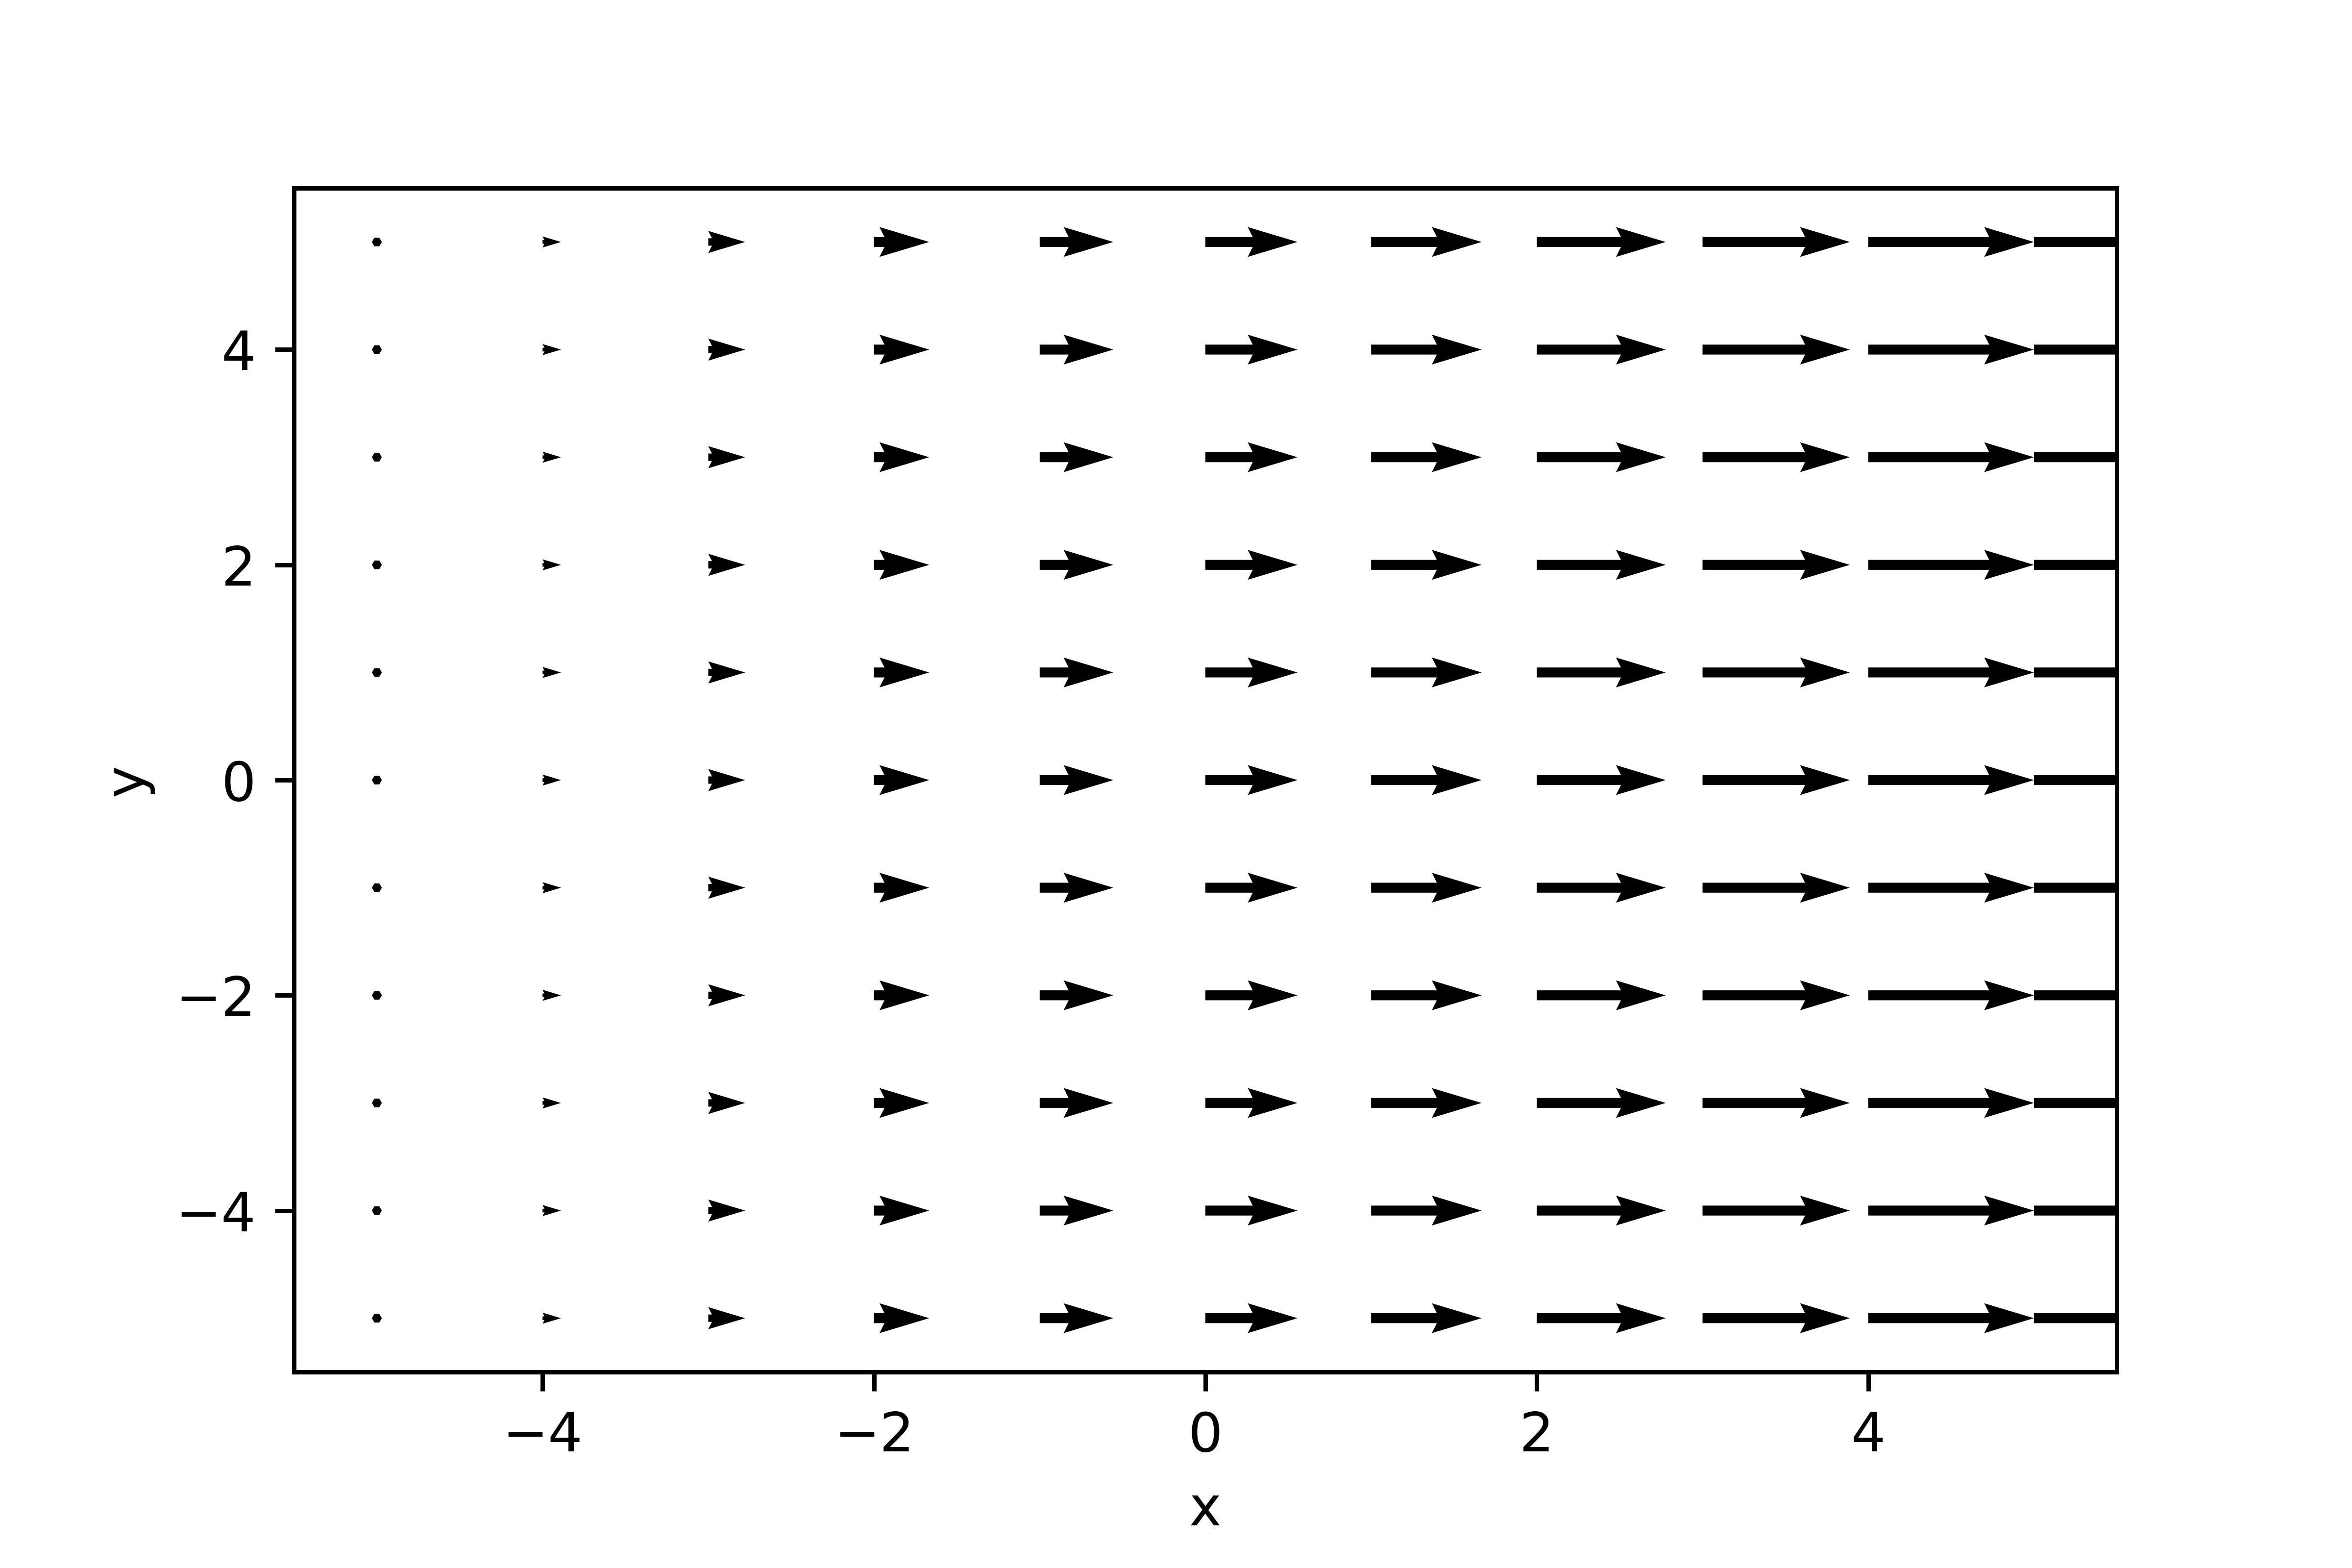
\includegraphics[height = 4cm]{figs/velocity_divergence.png}
\end{subfigure}
\begin{subfigure}[c]{.4\textwidth}
\centering
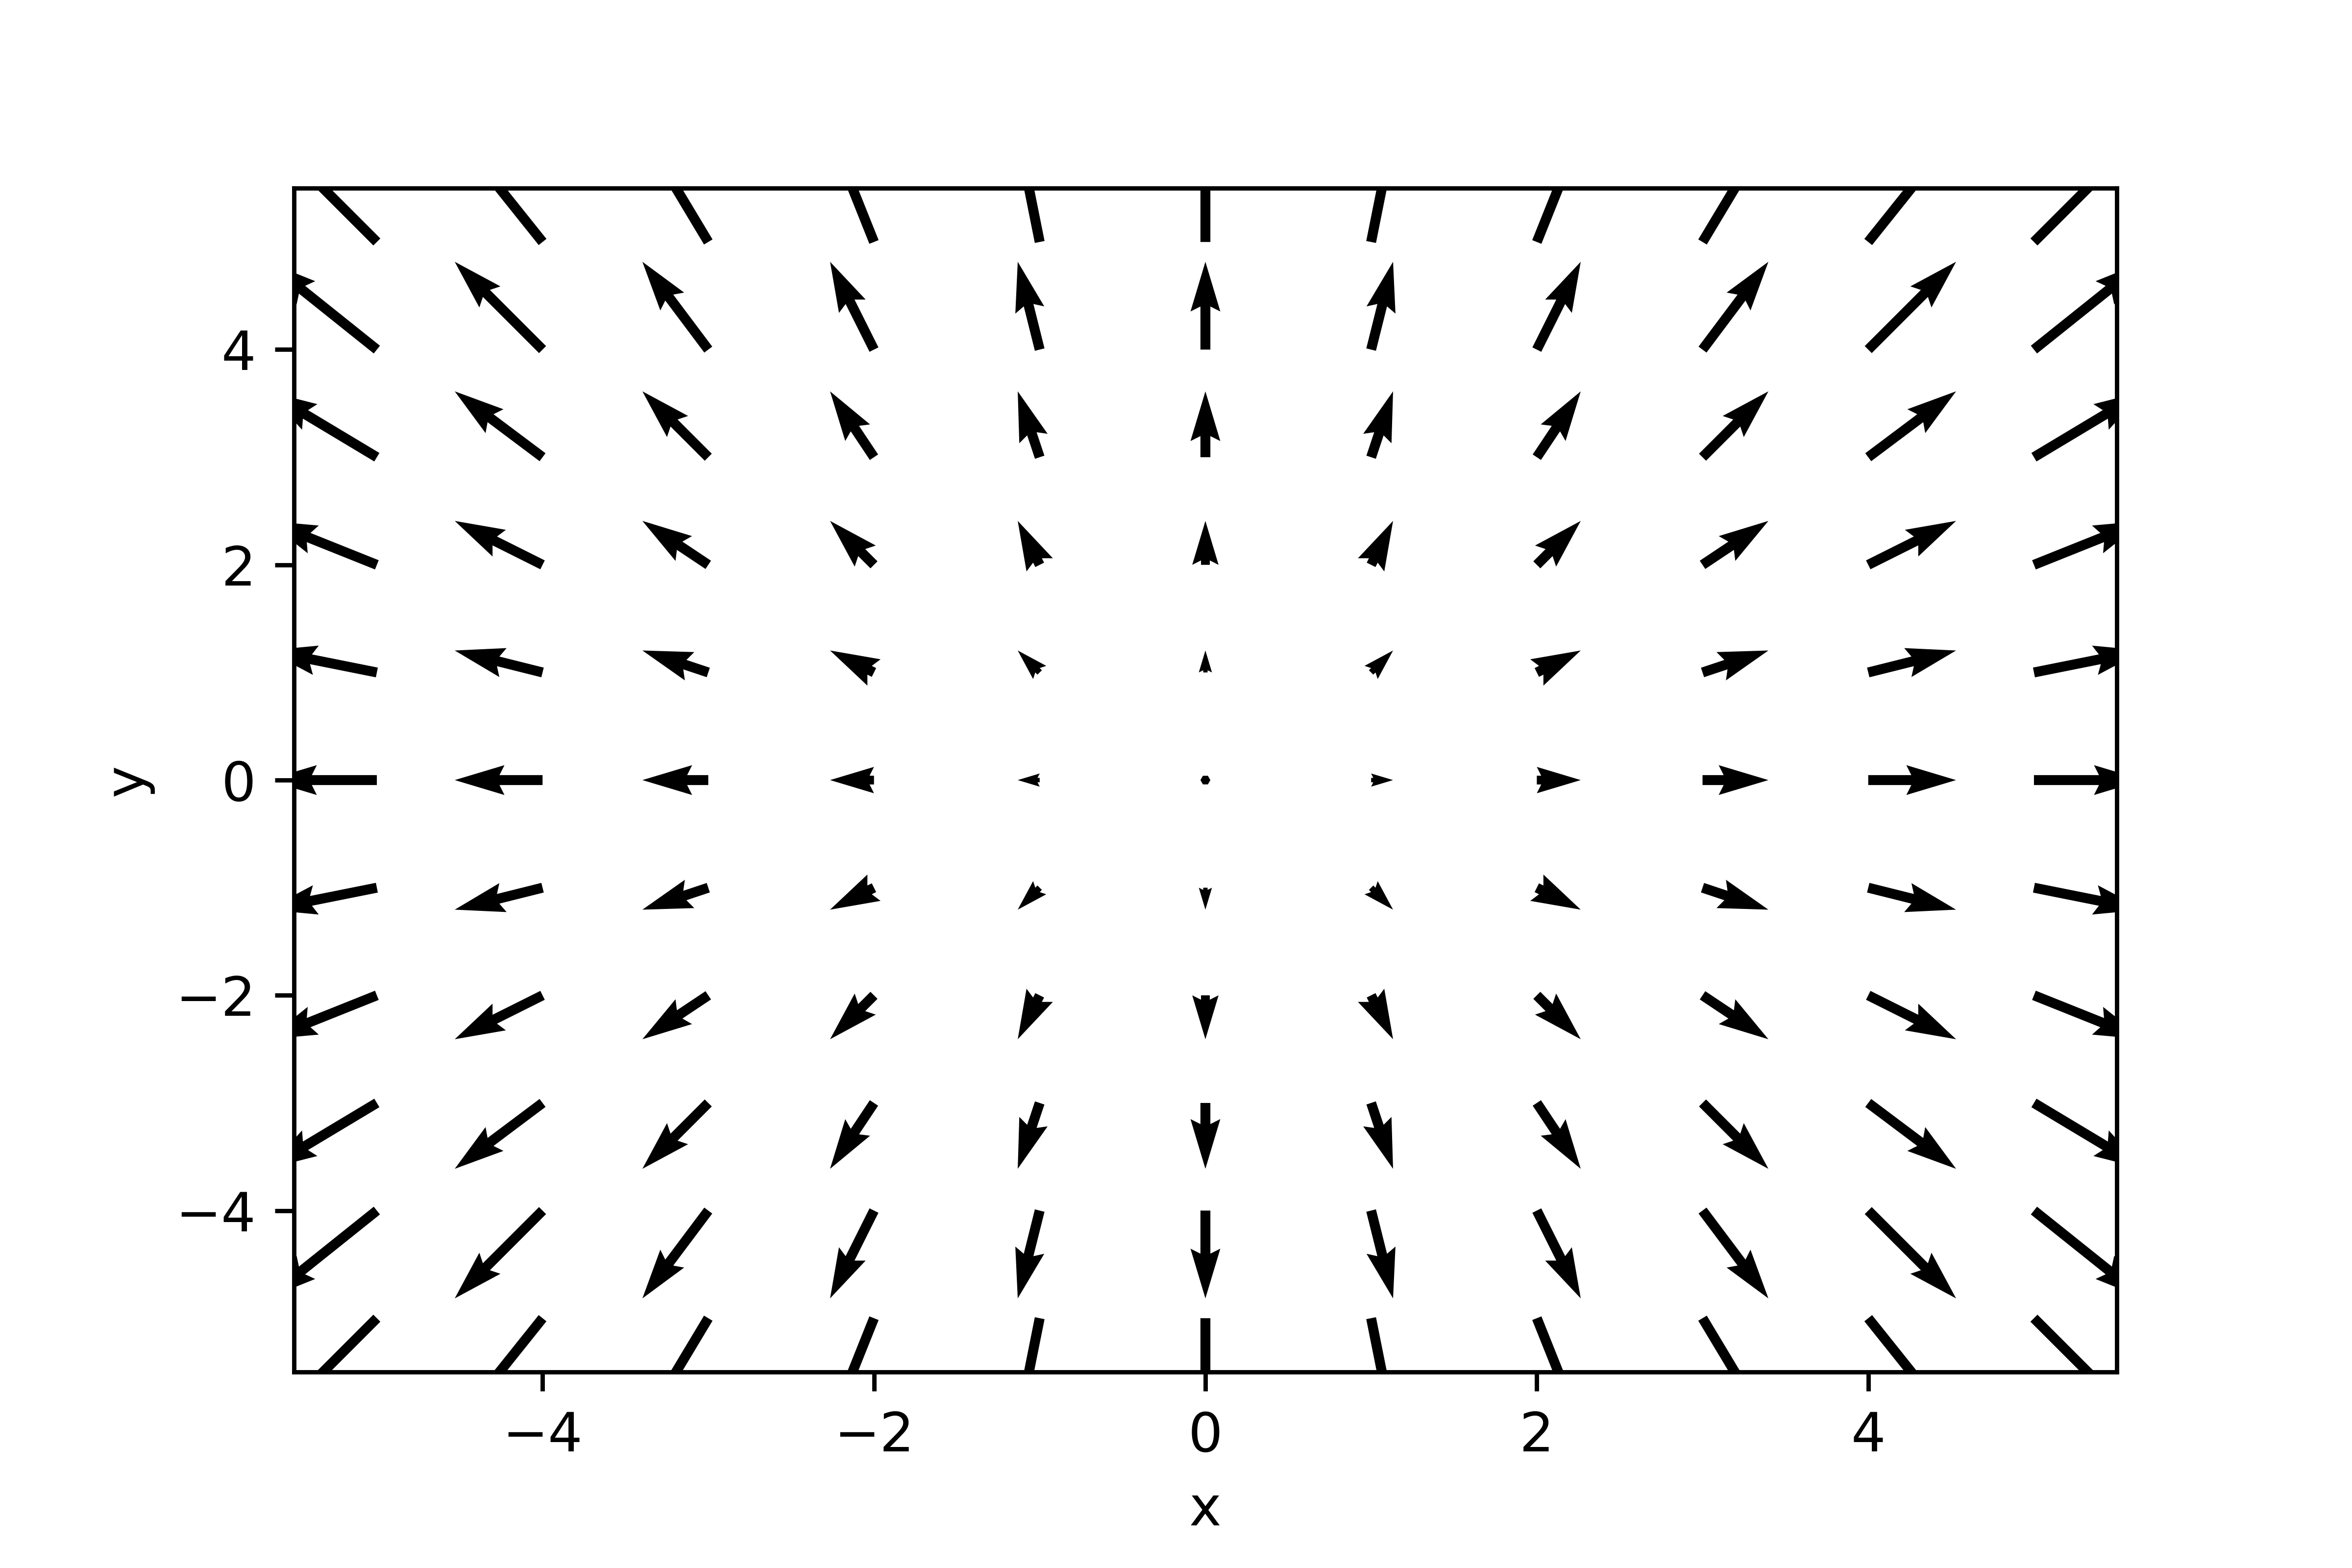
\includegraphics[height = 4cm]{figs/direction_divergence.png}
\end{subfigure}
\caption{Geschwindigkeitsdivergenz (links) und Richtungsdivergenz (rechts).}
\end{figure}

\subsection{Divergenzgleichung}
\label{sec:divergence_equation}\index{Divergenzgleichung}

Es gibt auch eine prognostische Gleichung für die Divergenz, die sogenannte \textit{Divergenzgleichung}. Die Impulsgleichung Glg. \eqref{eq:momentum_mod} lautet
%
\begin{align}
\frac{\partial\mathbf{v}}{\partial t} & = -\frac{1}{\rho}\nabla p + \mathbf{v}\times\mathbf{f} - \left(\mathbf{v}\cdot\nabla\right)\mathbf{v} + \mathbf{g} + \mathbf{f}_R.
\end{align}
%
Nun wendet man auf die einzelnen Terme den Operator $\nabla\cdot $ an:
%
\begin{align}
\nabla\cdot\frac{\partial\mathbf{v}}{\partial t} & \stackrel{\text{Glg. \eqref{eq:diff_op_rule_4}}}{=} \frac{\partial D}{\partial t}\\
\nabla\cdot\left(-\frac{1}{\rho}\nabla p\right) & \stackrel{\text{Glg. \eqref{eq:diff_op_rule_3}}}{=} \frac{1}{\rho^2}\nabla\rho\cdot\nabla p -\frac{1}{\rho}\Delta p\\
\nabla\cdot\left(\mathbf{v}\times\mathbf{f}\right) & \stackrel{\text{Glg. \eqref{eq:diff_op_rule_9}}}{=} \mathbf{f}\cdot\zetabi
\end{align}
%
Die Divergenz von $\mathbf{g}$ besteht aufgrund der Poisson-Gleichung nur aus dem Zentrifugalanteil. Da man in der Meteorologie jedoch für analytische Herleitungen meist von einem radialsymmetrischen Schwerefeld ausgeht, wird auch dieser Anteil vernachlässigt. Es gilt also
%
\begin{center}
\doublebox{\parbox{\textwidth}{
\begin{center}
\begin{align}
\frac{\partial D}{\partial t} & = \frac{1}{\rho^2}\nabla\rho\cdot\nabla p -\frac{1}{\rho}\Delta p + \mathbf{f}\cdot\zetabi - \nabla\cdot\left[\left(\mathbf{v}\cdot\nabla\right)\mathbf{v}\right] + \nabla\cdot\mathbf{f}_R.\label{eq:divergence_equation_1}
\end{align}
\end{center}
}}
\end{center}
%
Dies ist die Divergenzgleichung. Mit der Lamb-Transformation erhält man
%
\begin{align}
\nabla\cdot\left[\left(\mathbf{v}\cdot\nabla\right)\mathbf{v}\right] & = \Delta k - \nabla\cdot\left[\mathbf{v}\times\left(\nabla\times\mathbf{v}\right)\right] \stackrel{\text{Glg. \eqref{eq:diff_op_rule_9}}}{=} \Delta k - \zetabi^2 + \mathbf{v}\cdot\left(\nabla\times\zetabi\right)\nonumber\\
&\stackrel{\text{Glg. \eqref{eq:diff_op_rule_8}}}{=} \Delta k - \zetabi^2 - \mathbf{v}\cdot\left(\Delta\mathbf{v}\right) + \mathbf{v}\cdot\nabla D.
\end{align}
%
Dies führt auf eine weitere Form der Divergenzgleichung:
%
\begin{center}
\doublebox{\parbox{\textwidth}{
\begin{center}
\begin{align}
\frac{\partial D}{\partial t} & = \frac{1}{\rho^2}\nabla\rho\cdot\nabla p -\frac{1}{\rho}\Delta p + \mathbf{f}\cdot\zetabi - \Delta k + \zetabi^2\nonumber\\
&  +\mathbf{v}\cdot\left(\Delta\mathbf{v}\right) - \mathbf{v}\cdot\nabla D + \nabla\cdot\mathbf{f}_R\label{eq:divergence_equation_2}
\end{align}
\end{center}
}}
\end{center}

\subsubsection{Divergenzgleichung im p-System}
\label{sec:divergence_equation_im_p-system}\index{Divergenzgleichung!p-System}

Die Impulsgleichungen Glg.en \eqref{eq:x_momentum_simplified_simplified_p} - \eqref{eq:y_momentum_simplified_simplified_p} im p-System lauten vektoriell
%
\begin{align}
\frac{\partial\mathbf{v}_h}{\partial t} & = -\nabla\phi - f\mathbf{k}\times\mathbf{v}_h - \left(\mathbf{v}_h\cdot\nabla\right)\mathbf{v}_h - \omega\frac{\partial\mathbf{v}_h}{\partial p} + \nabla\cdot\mathbf{f}_R^{(H)}.
\end{align}
%
Es ist für die Hereitung sinnvoll, hier ein $\mathbf{g}$ zu addieren und $-\nabla\phi$ als dreidimensionalen Vektor zu interpretieren mit $-g$ in der z-Komponente. Somit ergibt eine Anwendung von $\nabla\cdot $ auf $-\nabla\phi + \mathbf{g} = -\Delta_h\phi$, wofür aber in der weiteren Herleitung einfach $\Delta\phi$ notiert wird. Durch Applizieren des Operators $\nabla\cdot $ auf die einzelnen Terme erhält man somit
%
\begin{align}
\nabla\cdot\frac{\partial\mathbf{v}_h}{\partial t}&\stackrel{\text{Glg. \eqref{eq:diff_op_rule_4}}}{=} \frac{\partial\delta}{\partial t}, \nonumber\\
- \nabla\cdot\nabla\phi & = -\Delta\phi, \nonumber\\
- \nabla\cdot\left(f\mathbf{k}\times\mathbf{v}_h\right)&\stackrel{\text{Glg. \eqref{eq:diff_op_rule_9}}}{=} -\mathbf{v}_h\cdot\left[\nabla\times\left(f\mathbf{k}\right)\right] + f\mathbf{k}\cdot\left(\nabla\times\mathbf{v}_h\right)\stackrel{\text{Glg. \eqref{eq:diff_op_rule_5}}}{=} - \mathbf{v}_h\cdot\left[-\mathbf{k}\times\nabla f + f\nabla\times\mathbf{k}\right] + f\zeta\nonumber\\
&= \mathbf{v}_h\cdot\left(\mathbf{k}\times\beta\mathbf{j}\right) + f\zeta = -u\beta + f\zeta, \nonumber\\
\nabla\cdot\left(-\omega\frac{\partial\mathbf{v}_h}{\partial p}\right)&\stackrel{\text{Glg. \eqref{eq:diff_op_rule_3}}}{=} -\omega\frac{\partial\delta}{\partial p} - \frac{\partial\mathbf{v}_h}{\partial p}\cdot\nabla\omega.
\end{align}
%
Somit folgt
%
\begin{center}
\doublebox{\parbox{\textwidth}{
\begin{center}
\begin{align}
\frac{\partial\delta}{\partial t} & = -\Delta\phi - u\beta + f\zeta - \nabla\cdot\left[\left(\mathbf{v}_h\cdot\nabla\right)\mathbf{v}_h\right] - \omega\frac{\partial\delta}{\partial p} - \frac{\partial\mathbf{v}_h}{\partial p}\cdot\nabla\omega + \nabla\cdot\mathbf{f}_R^{(H)}.\label{eq:divergence_equation_p_1}
\end{align}
\end{center}
}}
\end{center}
%
Dies ist die Divergenzgleichung im p-System. Mit der Lamb-Transformation erhält man
%
\begin{align}
\nabla\cdot\left[\left(\mathbf{v}_h\cdot\nabla\right)\mathbf{v}_h\right] & = \Delta k - \nabla\cdot\left[\mathbf{v}_h\times\left(\nabla\times\mathbf{v}_h\right)\right] \stackrel{\text{Glg. \eqref{eq:diff_op_rule_9}}}{=} \Delta k - \left(\nabla\times\mathbf{v}_h\right)^2 + \mathbf{v}_h\cdot\left(\nabla\times\left(\nabla\times\mathbf{v}_h\right)\right)\nonumber\\
&\stackrel{\text{Glg. \eqref{eq:diff_op_rule_8}}}{=} \Delta k - \left(\nabla\times\mathbf{v}_h\right)^2 - \mathbf{v}_h\cdot\left(\Delta\mathbf{v}_h\right) + \mathbf{v}_h\cdot\nabla\delta.
\end{align}
%
Dies führt auf eine weitere Form der Divergenzgleichung:
%
\begin{center}
\doublebox{\parbox{\textwidth}{
\begin{center}
\begin{align}
\frac{\partial\delta}{\partial t} & = -\Delta\phi - u\beta + f\zeta - \Delta k + \left(\nabla\times\mathbf{v}_h\right)^2 + \mathbf{v}_h\cdot\left(\Delta\mathbf{v}_h\right) - \mathbf{v}_h\cdot\nabla\delta\nonumber\\
& - \omega\frac{\partial\delta}{\partial p} - \frac{\partial\mathbf{v}_h}{\partial p}\cdot\nabla\omega + \nabla\cdot\mathbf{f}_R^{(H)}\label{eq:divergence_equation_p_2}
\end{align}
\end{center}
}}
\end{center}
%
Setzt man hier $\delta = \omega = 0$ ein, folgt die \index{Balancegleichung}\textit{Balancegleichung}
%
\begin{center}
\doublebox{\parbox{\textwidth}{
\begin{center}
\begin{align}
\Delta\phi & = - u\beta + f\zeta - \Delta k + \left(\nabla\times\mathbf{v}_h\right)^2 + \mathbf{v}_h\cdot\left(\Delta\mathbf{v}_h\right).\label{eq:balance_equation}
\end{align}
\end{center}
}}
\end{center}
%
Vernachlässigt man den letzten Term, erhält man die \textit{lineare Balancegleichung}\index{Balancegleichung!lineare}\index{lineare Balancegleichung}
%
\begin{align}
\Delta\phi = -u\beta + f\zeta.\label{eq:balance_equation_linear}
\end{align}
%
Verwendet man eine Stromfunktion $\psi$, folgt
%
\begin{align}
\Delta\phi = \beta\frac{\partial\psi}{\partial y} + f\Delta\psi.
\end{align}
%
Die Balancegleichung ermöglicht die Transformation $\psi\leftrightarrow\phi$.

Ein globales Einschichtmodell enthielte als einzige prognostische Variable die Stromfunktion, die prognostische Gleichung für diese wäre die Vorticitygleichung, der Wind wäre divergenuzfrei. Das Geopotential könnte bei Bedarf mittels Lösung der Balancegleichung diagnostiziert werden.

Es gibt also bei einem globalen Horizontalwindfeld immer einen Kompromiss aus Divergenzfreiheit und Geostrophie, ein realistisches synoptisch-skaliges Windfeld ist entweder divergenzfrei oder geostrophisch oder keins von beidem, jedoch nicht beides zugleich. Möchte man Schallwellen (enthalten Divergenz) und Schwerewellen (sind ageostrophisch) filtern (z. B. bei der Initialisierung), muss man daher ein Windfeld finden, was möglichst geostrophisch ist (und somit zum gemessenen Geopotential passt und keine Schwerewellen auslöst), und gleichzeitig möglichst divergenzfrei ist (und somit keine Schallwellen auslöst).

\section{Potentielle Vorticity}
\label{sec:potentielle_vorticity}\index{potentielle Vorticity}\index{Vorticity!potentielle}

\subsection{Ertel'scher Wirbelsatz}
\label{sec:ertel'scher_wirbelsatz}\index{Ertel'scher Wirbelsatz}\index{Wirbelsatz!Ertel'scher}

Man definiert eine Vorform der potentiellen Vorticity\index{potentielle Vorticity}\index{Vorticity!potentielle} $P_\psi$ durch
%
\begin{align}
P_\psi \coloneqq \alpha\etabi\cdot\nabla\psi, \label{eq:def_pot_vorticity_gen}
\end{align}
%
wobei $\alpha$ das spezifische Volumen sei und $\psi$ eine beliebige Funktion von Ort und Zeit. Differenziert man dies partiell nach der Zeit, erhält man
%
\begin{align}
\frac{\partial P_\psi}{\partial t} = \frac{\partial\alpha}{\partial t}\etabi\cdot\nabla\psi + \alpha\frac{\partial\left(\nabla\times\mathbf{v}\right)}{\partial t}\cdot\nabla\psi + \alpha\etabi\cdot\nabla\frac{\partial\psi}{\partial t}.
\end{align}
%
Zunächst wird Glg. \eqref{eq:vorticity_eq_3d} in Termen von $\alpha$ notiert
%
\begin{align}
\frac{\partial}{\partial t}\text{rot}\left(\mathbf{v}\right) & = \nabla p\times\nabla \alpha - \left(\mathbf{v}\cdot\nabla\right)\etabi - \etabi\nabla\cdot\mathbf{v} + \left(\etabi\cdot\nabla\right)\mathbf{v} + \nabla\times\mathbf{f}_R
\end{align}
%
In Absch. \ref{sec:vorticitygleichung} hat man durch Projektion dieser Gleichung auf die lokale Senkrechte $\mathbf{k}$ eine Gleichung für $\frac{\partial\zeta}{\partial t}$ hergeleitet, analog wird hier mit einer Projektion auf $\nabla\psi$ verfahren. Man rechnet zunächst mit Glg. \eqref{eq:diff_op_rule_11}

\begin{align}
\left(\etabi\cdot\nabla\right)\left(\mathbf{v}\cdot\nabla\psi\right) & = \nabla\psi\cdot\left[\left(\etabi\cdot\nabla\right)\mathbf{v}\right] + \mathbf{v}\cdot\left[\left(\etabi\cdot\nabla\right)\nabla\psi\right]\nonumber\\
\Rightarrow\nabla\psi\cdot\left[\left(\etabi\cdot\nabla\right)\mathbf{v}\right] & = \left(\etabi\cdot\nabla\right)\left(\mathbf{v}\cdot\nabla\psi\right) - \mathbf{v}\cdot\left[\left(\etabi\cdot\nabla\right)\nabla\psi\right],\\
\left(\mathbf{v}\cdot\nabla\right)\left(\etabi\cdot\nabla\psi\right) & = \etabi\cdot\left[\left(\mathbf{v}\cdot\nabla\right)\nabla\psi\right] + \nabla\psi\cdot\left[\left(\mathbf{v}\cdot\nabla\right)\etabi\right]\nonumber\\
\Rightarrow\nabla\psi\cdot\left[\left(\mathbf{v}\cdot\nabla\right)\etabi\right] & = \left(\mathbf{v}\cdot\nabla\right)\left(\etabi\cdot\nabla\psi\right) - \etabi\cdot\left[\left(\mathbf{v}\cdot\nabla\right)\nabla\psi\right].
\end{align}
%
Man erhält somit
%
\begin{align}
\alpha\frac{\partial\left(\nabla\times\mathbf{v}\right)}{\partial t}\cdot\nabla\psi & = \alpha\left(\nabla p\times\nabla\alpha\right)\cdot\nabla\psi - \alpha\left(\mathbf{v}\cdot\nabla\right)\left(\etabi\cdot\nabla\psi\right) + \alpha\etabi\cdot\left[\left(\mathbf{v}\cdot\nabla\right)\nabla\psi\right]\nonumber\\
&  -\alpha\left(\nabla\psi\cdot\etabi\right)\nabla\cdot\mathbf{v} + \alpha\left(\etabi\cdot\nabla\right)\left(\mathbf{v}\cdot\nabla\psi\right) - \alpha\mathbf{v}\cdot\left[\left(\etabi\cdot\nabla\right)\nabla\psi\right] + \alpha\mathbf{f}_R\cdot\nabla\psi.
\end{align}
%
Es folgt
%
\begin{align}
\frac{\partial P_\psi}{\partial t} & = \alpha\etabi\cdot\nabla\left(\frac{\partial\psi}{\partial t}\right) + \alpha\left(\nabla p\times\nabla\alpha\right)\cdot\nabla\psi - \alpha\left(\mathbf{v}\cdot\nabla\right)\left(\etabi\cdot\nabla\psi\right) + \alpha\etabi\cdot\left[\left(\mathbf{v}\cdot\nabla\right)\nabla\psi\right]\nonumber\\
&  -\alpha\left(\nabla\psi\cdot\etabi\right)\nabla\cdot\mathbf{v} + \alpha\left(\etabi\cdot\nabla\right)\left(\mathbf{v}\cdot\nabla\psi\right) - \alpha\mathbf{v}\cdot\left[\left(\etabi\cdot\nabla\right)\nabla\psi\right]\nonumber\\
&  +\frac{\partial\alpha}{\partial t}\etabi\cdot\nabla\psi + \alpha\mathbf{f}_R\cdot\nabla\psi\nonumber\\
& = \alpha\etabi\cdot\nabla\left(\frac{\partial\psi}{\partial t}\right) + \alpha\left(\nabla p\times\nabla\alpha\right)\cdot\nabla\psi - \alpha\left(\mathbf{v}\cdot\nabla\right)\left(\etabi\cdot\nabla\psi\right) + \alpha\etabi\cdot\left[\left(\mathbf{v}\cdot\nabla\right)\nabla\psi\right]\nonumber\\
&  +\alpha\left(\etabi\cdot\nabla\right)\left(\mathbf{v}\cdot\nabla\psi\right) - \alpha\mathbf{v}\cdot\left[\left(\etabi\cdot\nabla\right)\nabla\psi\right] - \left(\mathbf{v}\cdot\nabla\alpha\right)\left(\etabi\cdot\nabla\psi\right) + \alpha\mathbf{f}_R\cdot\nabla\psi.
\end{align}
%
Mit Glg. \eqref{eq:diff_op_rule_12} folgt
%
\begin{align}
\etabi\cdot\left[\left(\mathbf{v}\cdot\nabla\right)\nabla\psi\right] - \mathbf{v}\cdot\left[\left(\etabi\cdot\nabla\right)\nabla\psi\right] = 0.
\end{align}
%
Der \index{Ertel'scher Wirbelsatz}\index{Wirbelsatz!Ertel'scher}\textit{Ertel'sche Wirbelsatz} lautet somit
%
\begin{center}
\doublebox{\parbox{0.8\textwidth}{
\begin{center}
\begin{align}
\frac{\partial P_\psi}{\partial t} & = \alpha\etabi\cdot\nabla\left(\frac{\partial\psi}{\partial t}\right) + \alpha\left(\nabla p\times\nabla\alpha\right)\cdot\nabla\psi - \alpha\left(\mathbf{v}\cdot\nabla\right)\left(\etabi\cdot\nabla\psi\right)\nonumber\\
&  +\alpha\left(\etabi\cdot\nabla\right)\left(\mathbf{v}\cdot\nabla\psi\right) - \left(\mathbf{v}\cdot\nabla\alpha\right)\left(\etabi\cdot\nabla\psi\right) + \alpha\mathbf{f}_R\cdot\nabla\psi.\label{eq:ertel_vorticity_theorem}
\end{align}
\end{center}
}}
\end{center}
%
Mit der materiellen Ableitung kann man dies zu
%
\begin{center}
\doublebox{\parbox{0.8\textwidth}{
\begin{center}
\begin{align}
\md{P_\psi} & = \alpha\etabi\cdot\nabla\left(\md{\psi}\right) + \alpha\left(\nabla p\times\nabla\alpha\right)\cdot\nabla\psi + \alpha\mathbf{f}_R\cdot\nabla\psi\label{eq:ertel_vorticity_theorem_mat}
\end{align}
\end{center}
}}
\end{center}
%
umformulieren.

\subsection{Definition und Eigenschaften der PV}
\label{sec:definition_und_eigenschaften_der_pv}\index{potentielle Vorticity}\index{Vorticity!potentielle}

Die \textit{potentielle Vorticity} $P$ ist definiert durch
%
\begin{align}
P \coloneqq\alpha\etabi\cdot\nabla\theta, 
\end{align}
%
sie entsteht also, indem man in Glg. \eqref{eq:def_pot_vorticity_gen} für $\psi$ die potentielle Temperatur $\theta$ einsetzt. Diese ist eine Funktion von Druck and spezifischem Volumen, also verschindet in Glg. \eqref{eq:ertel_vorticity_theorem} der Term mit dem Vektorprodukt. Bei adiabatischen Prozessen gilt also, 

\begin{center}
\doublebox{\parbox{0.8\textwidth}{
\begin{center}
\begin{align}
\frac{\partial P}{\partial t} & = -\alpha\left(\mathbf{v}\cdot\nabla\right)\left(\etabi\cdot\nabla\psi\right) - \left(\etabi\cdot\nabla\psi\right)\left(\mathbf{v}\cdot\nabla\alpha\right) + \alpha\mathbf{f}_R\cdot\nabla\theta.
\end{align}
\end{center}
}}
\end{center}
%
in diesem Fall ist die potentielle Vorticity also bis auf die Reibung eine Erhaltungsgröße:
%
\begin{center}
\doublebox{\parbox{0.8\textwidth}{
\begin{center}
\begin{align}
\md{P} & =  \alpha\mathbf{f}_R\cdot\nabla\theta
\end{align}
\end{center}
}}
\end{center}
%
Für die potentielle Vorticity gilt mit Glg. \eqref{eq:rot_local}
%
\begin{align}
P & = \alpha\etabi\cdot\nabla\theta = \alpha\mathbf{f}\cdot\nabla\theta\nonumber\\
&  + \alpha\left[\left(\frac{\partial w}{\partial y} - \frac{\partial v}{\partial z} - \frac{v}{r}\right)\frac{\partial\theta}{\partial x} + \left(\frac{\partial u}{\partial z} - \frac{\partial w}{\partial x} + \frac{u}{r}\right)\frac{\partial\theta}{\partial y} + \left(\frac{\partial v}{\partial x} - \frac{\partial u}{\partial y} - \frac{u\tan\left(\varphi\right)}{r}\right)\frac{\partial\theta}{\partial z}\right].
\end{align}
%
Hier macht man nun folgende Näherungen:
%
\begin{itemize}
\item shallow atmosphere (s. Absch. \ref{sec:shallow_atmosphere})
\item Vernachlässigung der Vertikalgeschwindigkeit bei der Berechnung der Rotation des Windfeldes
\end{itemize}
%
Dann erhält man
%
\begin{align}
P & = \alpha\eta\frac{\partial\theta}{\partial z} + \alpha\left[-\frac{\partial v}{\partial z}\frac{\partial\theta}{\partial x} + \frac{\partial u}{\partial z}\frac{\partial\theta}{\partial y}\right].\label{eq:pot_vort_approx}
\end{align}
%
In einer hydrostatischen Atmosphäre kann man in Glg. \eqref{eq:pot_vort_approx} die vertikalen Ableitungen ins p-System transformieren:
%
\begin{align}
P & = -gf\frac{\partial\theta}{\partial p} - g\left(\frac{\partial v}{\partial x} - \frac{\partial u}{\partial y} - \frac{u\tan\left(\varphi\right)}{a}\right)\frac{\partial\theta}{\partial p} + g\left[\frac{\partial v}{\partial p}\frac{\partial\theta}{\partial x} - \frac{\partial u}{\partial p}\frac{\partial\theta}{\partial y}\right]\label{eq:pot_vort_approx_hydrostat}
\end{align}
%
Transformiert man hier die horizontalen Ableitungen mit Glg. \eqref{eq:trans_gen_2} auf eine generalisierte Vertikalkoordinte $\mu$, folgt
%
\begin{align}
\frac{P}{g} & = \dotsc\newvline_\mu - \left(\frac{\partial\mu}{\partial x}\right)_z\frac{\partial v}{\partial \mu}\frac{\partial\theta}{\partial p} + \left(\frac{\partial\mu}{\partial y}\right)_z\frac{\partial u}{\partial \mu}\frac{\partial\theta}{\partial p} + \frac{\partial v}{\partial p}\frac{\partial\theta}{\partial\mu}\left(\frac{\partial\mu}{\partial x}\right)_z - \frac{\partial u}{\partial p}\frac{\partial\theta}{\partial \mu}\left(\frac{\partial\mu}{\partial y}\right)_z, 
\end{align}
%
wobei die formal zu Glg. \eqref{eq:pot_vort_approx_hydrostat} gleichen Terme abgekürzt wurden. Die formal neuen Terme verschwinden in den beiden Fällen $\mu = p, \theta$. Somit kann man für die potentielle Vorticity notieren
%
\begin{align}
P & = -g\eta_p\frac{\partial\theta}{\partial p} + g\left[\frac{\partial v}{\partial p}\left(\frac{\partial\theta}{\partial x}\right)_p - \frac{\partial u}{\partial p}\left(\frac{\partial\theta}{\partial y}\right)_p\right], 
\end{align}
%
wobei der Index $p$ bedeutet, dass partielle Ableitungen im p-System zu bilden sind. In isentropen Koordinaten bleibt nur der erste Term bestehen, 
%
\begin{align}
P & = -g\eta_\theta\left(\frac{\partial p}{\partial\theta}\right)^{-1} \equiv \frac{\eta_\theta}{\sigma_\theta}, 
\end{align}
%
wobei die \textit{hydrostatische Stabilität im $\theta-$System}\index{hydrostatische Stabilität im $\theta-$System}\index{$\theta-$System!hydrostatische Stabilität}, definiert durch
%
\begin{align}
\sigma_\theta \coloneqq -\frac{1}{g}\frac{\partial p}{\partial\theta}, 
\end{align}
%
eingeführt wurde.

\chapter{\normalfont\textsc{Wellen und Instabilitäten}}
\label{chap:wellen_und_instabilitaeten}\index{Welle}\index{Instabilität}

Die Bewegungsgleichungen haben Wellenlösungen. Diese erhält man durch Einsetzen eines komplexen harmonischen Ansatzes in das jeweilige Gleichungssystem und Suchen nach nichttrivialen Lösungen. Es findet eine Unterscheidung in barotrope und barokline Wellen statt. In diesem Kapitel werden die advektiven Terme linearisiert, um die Gleichungen leichter behandeln zu können, dabei wird gelegentlich aufgrund der klimatologischen Relevanz ein zonaler Grundstrom aufgenommen.

\section{Kinematik}
\label{sec:kinematik}\index{Kinematik!Welle}\index{Welle!Kinematik}

Als Wellen bezeichnet man räumlich und zeitlich periodische Änderungen. Der maximale betragsmäßige Ausschlag aus der Ruhelage ist die Amplitude. Die Zeit $T > 0$ bis zur Wiederholung des Bewegungsmusters an einem festgehaltenen Ort bezeichnet man als Periodendauer, ihr Inverses ist die Frequenz $f$. Die Kreisfrequenz $\omega$ ist definiert als
%
\begin{align}
\omega \coloneqq 2\pi f = \frac{2\pi}{T}.
\end{align}
%
Analog ist die Wellenlänge $\lambda > 0$ die Länge, nach der sich das Bewegungsmuster wiederholt. Wellenzahl $\kappa$ und Kreiswellenzahl $k$ sind anlog zu Frequenz und Kreisfrequenz definiert durch
%
\begin{align}
\kappa \coloneqq \frac{1}{\lambda}, && k \coloneqq \frac{2\pi}{\lambda}.
\end{align}
%
Eine Welle der Größe $a$ wird beschrieben durch eine Gleichung der Form
%
\begin{align}
a\left(x, t\right) = Af\left(kx - \omega t + \varphi\right).
\end{align}
%
Dabei ist $f$ eine reell- oder komplexwertige, $2\pi-$periodische Funktion, d. h. $f\left(\xi + 2\pi\right) = f\left(\xi\right)$ für jedes $\xi\in\mathbb{R}$. Dies kann, muss aber keine trigonometrische Funktion sein. $f$ wird häufig komplexwertig gewählt, z. B. $f(x) = \exp(ix)$, falls dies die mathematische Beschreibung abkürzt oder anschaulicher macht. Bevor man jedoch Größen berechnet, die man mit Messgrößen vergleichen möchte, muss man allerdings alles auf die reelle Achse projizieren. Das Argument $kx - \omega t + \varphi$ nennt man auch die \textit{Phase} der Welle, in der komplexen Ebene ist dies der Winkel, den die Zahl mit der Realachse einschließt. $\varphi$ ist dabei die Phasenverschiebung, die ermöglicht, dass die Phase der Welle bei $x, t = 0$ nicht gleich Null ist. Man kann bei Herleitungen häufig auf $\varphi$ verzichten, indem man die Zeit- oder Ortskoordinate entsprechend verschiebt. $k$ und $\omega$ können auch imaginäre Anteile haben, so z. B. bei Wellen, die exponentiell in ein Medium hineinpropagieren (sog. \textit{evaneszente Wellen}\index{Welle!evaneszente}\index{evaneszente Welle}), oder bei Instabilitäten, bei denen die Amplitude über einen gewissen hinweg Zeitraum exponentiell anwächst. Genauso kann auch der Vorfaktor $A$ komplex sein, und so eine Phasenverschiebung beinhalten.

Im Allgemeinen kann sich eine Welle auch in einem dreidimensionalen Raum fortpflanzen, in diesem Fall schreibt man zunächst allgemein
%
\begin{align}
a\left(\mathbf{r}, t\right) = Af\left(\phi\left(\mathbf{r}, t\right)\right)
\end{align}
%
mit $\phi = \phi\left(\mathbf{r}, t\right)$ als Phasenfunktion. Die Phasenfunktion kann zum Beispiel die Gestalt
%
\begin{align}
\varphi\left(\mathbf{r}, t\right) = \mathbf{k}\cdot\mathbf{r} - \omega t\label{eq:phase_velocity_deriv}
\end{align}
%
haben, hierbei bezeichnet man $\mathbf{k} = \left(k_x, k_y, k_z\right)^T$ als den Wellenvektor. Sein Betrag ist gleich der Kreiswellenzahl, er zeigt in Ausbreitungsrichtung der Welle. Leitet man Glg. \eqref{eq:phase_velocity_deriv} nach der Zeit ab, folgt
%
\begin{align}
\frac{d\varphi\left(\mathbf{r}, t\right)}{dt} = \mathbf{k}\cdot\frac{d\mathbf{r}}{dt} - \omega
\end{align}
%
Setzt man die linke Seite gleich Null, bewegt sich also mit einem Punkt konstanter Phase mit, und wählt eine Trajektorie parallel zu $\mathbf{k}$, so erhält man die Phasengeschwindigkeit
%
\begin{center}
\doublebox{\parbox{0.8\textwidth}{
\begin{center}
\begin{align}
c = \frac{\omega}{k} = \frac{\lambda}{T} = \lambda f.
\end{align}
\end{center}
}}
\end{center}
%
Die Abhängigkeit
%
\begin{align}
\omega = \omega\left(k\right)
\end{align}
%
bezeichnet man als \index{Dispersionsrelation}\textit{Dispersionsrelation}. Nun betrachtet man die Übelagerung $f\left(x, t\right) = f_1\left(x, t\right) + f_2\left(x, t\right)$ zweier Wellen:
%
\begin{align}
f_1\left(x, t\right) & = -\cos\left(k_1x - \omega_1t\right)\\
f_1\left(x, t\right) & = \cos\left(k_2x - \omega_2t\right)\\
f\left(x, t\right) & = -\cos\left(k_1x - \omega_1t\right) + \cos\left(k_2x - \omega_2t\right)
\end{align}
%
Mit Glg. \eqref{eq:trigo_add_lemma_1} folgt
%
\begin{align}
-\cos\left(\alpha\right) + \cos\left(\beta\right) & = 1 - \cos\left(\alpha\right) - 1 + \cos\left(\beta\right) = 2\sin^2\left(\frac{\alpha}{2}\right) - 2\sin^2\left(\frac{\beta}{2}\right)\nonumber\\
& = 2\sin^2\left(\frac{\alpha}{2}\right) - 2\sin^2\left(\frac{\alpha}{2}\right)\sin^2\left(\frac{\beta}{2}\right) - 2\sin^2\left(\frac{\beta}{2}\right) + 2\sin^2\left(\frac{\alpha}{2}\right)\sin^2\left(\frac{\beta}{2}\right)\nonumber\\
& = 2\left[\sin^2\left(\frac{\alpha}{2}\right)\cos^2\left(\frac{\beta}{2}\right) - \cos^2\left(\frac{\alpha}{2}\right)\sin^2\left(\frac{\beta}{2}\right)\right]\nonumber\\
& = 2\left[\sin\left(\frac{\alpha}{2}\right)\cos\left(\frac{\beta}{2}\right) - \cos\left(\frac{\alpha}{2}\right)\sin\left(\frac{\beta}{2}\right)\right]\left[\sin\left(\frac{\alpha}{2}\right)\cos\left(\frac{\beta}{2}\right) + \cos\left(\frac{\alpha}{2}\right)\sin\left(\frac{\beta}{2}\right)\right]\nonumber\\
& = 2\sin\left(\frac{\alpha - \beta}{2}\right)\sin\left(\frac{\alpha + \beta}{2}\right).
\end{align}
%
Es gilt also
%
\begin{align}
f\left(x, t\right) & = 2\sin\left(\frac{\Delta k x - \Delta\omega t}{2}\right)\sin\left(\newoverline{k}x - \newoverline{\omega}t\right)
\end{align}
%
mit
%
\begin{align}
\Delta k \coloneqq k_2 - k_1, && \Delta\omega \coloneqq \omega_2 - \omega_1,\\
\newoverline{k} \coloneqq \frac{k_1 + k_2}{2}, && \newoverline{\omega} \coloneqq \frac{\omega_1 + \omega_2}{2}.
\end{align}
%
Die Einhüllende $\sin\left(\frac{\Delta k x - \Delta\omega t}{2}\right)$ bewegt sich also mit der Geschwindigkeit
%
\begin{align}
v_e = \frac{\Delta\omega}{\Delta k}.
\end{align}
%
Man definiert daher die \textit{Gruppengeschwindigkeit}\index{Gruppengeschwindigkeit} $c_{\text{gr}}$ durch
%
\begin{align}
c_{\text{gr}} \coloneqq \frac{\partial\omega}{\partial k}.
\end{align}
%
Sie kann also aus der Dipersionsrelation abgeleitet werden. Es ist die Geschwindigkeit, mit der sich Wellenpakete bewegen, mit der also Energie transportiert wird. Ist
%
\begin{align}
c_{\text{gr}} = c
\end{align}
%
unabhängig von $k$, so bezeichnet man die Welle als \textit{dispersionsfrei}. Man kann die Gruppengeschwindigkeit vektoriell zu
%
\begin{center}
\doublebox{\parbox{0.8\textwidth}{
\begin{center}
\begin{align}
c_{\text{gr}} = \nabla_{\mathbf{k}}\omega.
\end{align}
\end{center}
}}
\end{center}
%
verallgemeinern. Mit $\omega = ck$ kann man schreiben
%
\begin{align}
c_{\text{gr}} & = \frac{d\omega}{dk} = c + k\frac{dc}{dk} = c + k\frac{d\lambda}{dk}\frac{dc}{d\lambda} = c - \frac{2\pi}{k}\frac{dc}{dy} = c - \lambda\frac{dc}{d\lambda}.
\end{align}
%
Im Fall $dc/d\lambda < 0$ spricht man von \textit{anormaler Dispersion}\index{anormale Dispersion}\index{Dispersion!anormale}. In diesem Fall propagiert die Energie schneller als die Phasengeschwindigkeit. Im Fall
%
\begin{align}
\frac{dc}{d\lambda}\lambda > c \Leftrightarrow \frac{dc}{d\lambda} > \frac{c}{\lambda} = f
\end{align}
%
bzw.
%
\begin{align}
\frac{d\omega}{dk} < 0
\end{align}
%
propagiert die Energie in einer dem Wellenvektor entgegengesetzten Richtung.

Lässt der Charakter einer Welle dies zu, kategorisiert man sie entweder als \index{Longitudinalwelle}\textit{Longitudinalwelle}, bei der die Oszillatoren parallel zum Wellenvektor schwingen, oder als \index{Transversalwelle}\textit{Transversalwelle}, bei der sie senkrecht dazu schwingen. Bei mechanischen Transversalwellen führt man als weiter kinematische Größen die \index{Wellenhöhe}\textit{Wellenhöhe} $H$ als doppelter Amplitude sowie die \index{Steilheit}\textit{Steilheit} $S$ einer Welle ein, welche durch
%
\begin{align}
S \coloneqq \frac{H}{\lambda}
\end{align}
%
definiert ist und somit dimensionslos ist.

\section{Begründung der Linearisierung}
\label{sec:begruendung_der_linearisierung}\index{Linearisierung!Wellengleichung}

Man kann sich die Bewegungen in der Atmosphäre als in sechs Anteile aufgeteilt denken:
%
\begin{itemize}
\item quasigeostrophische, quasidivergenzfreie Bewegungen inkl. Rossby-Wellen
\item Schwerellen
\item Konvektion
\item Reibungswind
\item Frontenzirkulation
\item mikroskalige Turbulenz
\item (Schallwellen, wobei diese keine meteorologische Relevanz haben, aber in Modellen als Lärm auftreten können)
\end{itemize}
%
Zu einem gegebenen Zeitpunkt ist diese Aufteilung konzeptionell meist möglich. Leider gilt dies nicht für die Vorhersage, da zwischen all diesen Bereichen Wechselwirkungen existieren. Man spricht in so einem Fall auch von Nichtlinearität. Sind $A, B$ zwei Phänomene und ist $f\left(A + B\right)$ beispielsweise eine Vorhersage, so gilt im Allgemeinen
%
\begin{align}
f\left(A + B\right) \not = f\left(A\right) + f\left(B\right), 
\end{align}
%
der Gesamteffekt von $A + B$ ist also nicht die Summe der Einzeleffekte $A, B$, da $f$ keine lineare Abbildung ist.

Bei der Suche nach analytischen Lösungen eines nichtlinearen Gleichungssystems, insbesondere bei der Suche nach Wellenlösungen, ist man jedoch sehr interessiert an einer Linearisierung. Dies ist mal mehr mal weniger gerechtfertigt. Man geht hierzu davon aus, dass für eine Größe $A = A_0 + A'$ mit $A_0$ als Hintergrundzustand und $A'$ als Störung gilt
%
\begin{align}
\mathcal{O}\left(A_0\right) = \mathcal{O}\left(A'\right) + 1, 
\end{align}
%
daher gilt
%
\begin{align}
\mathcal{O}\left(A'^2\right) = \mathcal{O}\left(A_0\right) - 2.
\end{align}
%
Man vernachlässigt daher alle Terme, in denen Produkte der Störungen auftreten. Dies führt zu einer Linearisierung des Gleichungssystems. Für die Ableitungen gilt unter Annahme einer ebenen Welle in x-Richtung mit Kreisfrequenz $\omega$ und Kreiswellenzahl $k$, die nur die Störungen betrifft
%
\begin{align}
\mathcal{O}\left(\frac{\partial A'}{\partial t}\right) & = \mathcal{O}\left(\omega A'\right),\\
\mathcal{O}\left(\frac{\partial A'}{\partial x}\right) & = \mathcal{O}\left(kA'\right)\\
\mathcal{O}\left(\frac{\frac{\partial A'}{\partial t}}{A\frac{\partial A'}{\partial x}}\right) & = \mathcal{O}\left(\frac{\omega}{Ak}\right) = \mathcal{O}\left(\frac{c}{A}\right).\label{eq:bed_lin_wellglg}
\end{align}
%
Aus Glg. \eqref{eq:bed_lin_wellglg} folgt, dass man die advektiven Terme vernachlässigen kann, wenn die Phasengeschwindigkeit $c = \frac{\omega}{k}$ viel größer als die Fluidteilchengeschwindigkeit ist.

Ist es möglich, alle nichtlinearen Terme eines Gleichungssystems zu eliminieren, so weiß man, dass sich zwei unabhängige Lösungen dieses Gleichungssystems nicht beeinflussen. Beispiele sind Schallwellen und elektromagnetische Wellen. Die Linearität dieser Systeme macht die unabhängige Überlagerung verschiedener Geräusche oder Signale möglich.

\subsection{Beispiel: Schallwellen}
\label{sec:bespiel_schallwellen}\index{Schallwelle}

Schallwellen sind Kompressionswellen, jedoch lassen sich dabei aufgrund der Adiabatie Drücke und Dichten eindeutig aufeinander abbilden. Es wird eine sich in x-Richtung ausbreitende Welle betrachtet. Der Störungsansatz für Geschwindigkeit und Dichte lautet
%
\begin{align}
u = U + u', && \rho = \rho_0 + \rho'.
\end{align}
%
Das Gleichungssystem lautet mit den abkürzenden Ersetzungen
%
\begin{align}
\rho' &\to \rho,\\
u' &\to u
\end{align}
%
und den im vorigen Abschnitt hergeleiteten Näherungen somit
%
\begin{align}
\frac{\partial u}{\partial t} + U\frac{\partial u}{\partial x} & = -\frac{1}{\rho _0}\frac{\partial p}{\partial x}\label{eq:schall_1}\\
\frac{\partial\rho}{\partial t} + U\frac{\partial \rho}{\partial x} & =  - \rho _0\frac{\partial u}{\partial x}\label{eq:schall_2}\\
\rho(p) & = \rho _0\left(\frac{p}{p_0}\right)^{c_v/c_p}
\end{align}
%
Bei der ersten Gleichung handelt es sich um die Impulsgleichung, die zweite ist die Kontinuitätsgleichung und die dritte ist die Gleichung für die potentielle Dichte Glg. \eqref{eq:pot_dichte}. Um in Glg. \eqref{eq:schall_2} die Dichteänderung durch den Druck auszudrücken, benutzt man die Kettenregel:
%
\begin{align}
\frac{\partial\rho}{\partial t} = \frac{\partial\rho}{\partial p}\frac{\partial p}{\partial t} = \frac{\rho_0c_v}{p_0c_p}\left(\frac{p}{p_0}\right)^{c_v/c_p - 1}\frac{\partial p}{\partial t} = \frac{\rho_0c_v}{p_0c_p}\frac{\partial p}{\partial t}, 
\end{align}
%
analog für $\frac{\partial}{\partial x}$. Die Ableitung der Dichte nach dem Druck wurde dabei an der Stelle $p = p_0$ ausgewertet, weil die Druckschwankungen sehr klein sind. Nun macht man einen Ansatz
%
\begin{align}
u = u_0\exp\left[i\left(kx - \omega t\right)\right], && p = P\exp\left[i\left(kx - \omega t\right)\right]
\end{align}
%
mit eventuell komplexen Amplituden $u_0, P$. Setzt man dies in das Gleichungssystem ein, folgt
%
\begin{align}
- i\omega u_0 + Uiku_0 & = -\frac{1}{\rho_0}ikP,\\
- \frac{\rho_0c_v}{p_0c_p}i\omega P + Uik\frac{\rho_0c_v}{p_0c_p}P & = -\rho_0 iku_0\nonumber\\
\Leftrightarrow - i\omega P + UikP & = -\frac{p_0c_p}{c_v}iku_0.
\end{align}
%
Als Matrixgleichung wird dies zu
%
\begin{align}
\left(\begin{array}{cc}
- i\omega + Uik&\frac{1}{\rho_0}ik\\
ik\frac{p_0c_p}{c_v}& -i\omega + Uik
\end{array}\right)\left(\begin{array}{c}
u_0\\
P
\end{array}\right) = \mathbf{0}.
\end{align}
%
Nichttriviale Lösungen existieren für
%
\begin{align}
\left(\omega - Uk\right)^2 - k^2\frac{p_0c_p}{\rho_0c_v} = 0\Leftrightarrow \omega = Uk\pm k\sqrt{\frac{p_0c_p}{\rho_0c_v}}.
\end{align}
%
Für die Phasengeschwindigkeit $c$ folgt also
%
\begin{center}
\doublebox{\parbox{0.8\textwidth}{
\begin{center}
\begin{align}
c = U\pm \sqrt{R_dT\kappa}.\label{eq:velocity_sound}
\end{align}
\end{center}
}}
\end{center}
%
Hierbei wurde die Zustandsgleichung eingesetzt, $T$ ist die Gleichgewichtstemperatur und $\kappa = c_p/c_v>1$ der Adiabatenexponent\index{Adiabatenexponent}\index{Isentropenexponent}. Der Wert von $c$ ist jedoch auch von der Feuchte abhängig. Man könnte also über eine Messung der Schallgeschwindigkeit durch Kombination mit einer Temperaturmessung die Feuchte bestimmen. Anzumerken ist, dass Schallwellen dispersionsfrei sind, die Phasengeschwindigkeit jedoch orts- und zeitabhängig ist, da sie von der Temperatur und der Feuchte abhängt.

\section{Barotrope Wellen}
\label{sec:barotrope_wellen}\index{barotrope Welle}\index{Welle!barotrope}

Die SWEs bilden das einfachst mögliche dynamische Gleichungssystem, deshalb werden zunächst die Wellenlösungen dieses Systems untersucht.

\subsection{Sub-Poincaré-Wellen}
\label{sec:sub-poincare-wellen}\index{Sub-Poincaré-Welle}\index{Welle!Sub-Poincaré}

Man geht an dieser Stelle von der Abwesenheit eines zonalen Grundstroms $U = 0$ aus, o. B. d. A. richtet man außerdem die x-Richtung am Wellenvektor aus, sodass das linearisierte Gleichungssystem hier
%
\begin{align}
\frac{\partial u}{\partial t} & = -g\frac{\partial\eta}{\partial x}, \label{eq:deep_1}\\
\frac{\partial u}{\partial x} + \frac{\partial w}{\partial z} & = 0\label{eq:deep_2}
\end{align}
%
lautet. Man geht von einer homogenen Tiefe $D > 0$ aus und fordert als Randbedingung

\begin{align}
w\left(z = -D\right) \hastobe 0.\label{eq:deep_deriv_1}
\end{align}
%
Es werden nun die Ansätze
%
\begin{align}
u = U\left(z\right)\exp\left(ikx - i\omega t\right), && w = W\left(z\right)\exp\left(ikx - i\omega t\right).
\end{align}
%
Die Oberflächenauslenkung $\eta$ und die Vertikalgeschwindigkeit $w$ hängen über
%
\begin{align}
\frac{\partial\eta}{\partial t}\left(z = 0\right) & \hastobe w\left(z = 0\right),\\
\Rightarrow -i\omega\hat{\eta} & = W\left(0\right)\label{eq:deep_deriv_2}
\end{align}
%
zusammen, wobei $\hat{\eta}$ die Amplitude der Oberflächenauslenkung ist. Glg. \eqref{eq:deep_1} ergibt somit bei $z = 0$
%
\begin{align}
-i\omega U\left(0\right) = g\frac{k}{\omega}W\left(0\right) \Rightarrow \omega^2 = igk\frac{W\left(0\right)}{U\left(0\right)}.\label{eq:deep_disp_pre}
\end{align}
%
Aus Glg. \eqref{eq:deep_2} folgt
%
\begin{align}
ikU\left(z\right) + W' = 0 \Rightarrow W' = -ikU.
\end{align}
%
Dies und die Glg.en \eqref{eq:deep_deriv_1} und \eqref{eq:deep_deriv_2} ist durch
%
\begin{align}
U\left(z\right) & = \frac{\hat{\eta}\omega}{\sinh\left(kD\right)}\cosh\left[k\left(D + z\right)\right],\label{eq:u_vert_mod_short_waves}\\
W\left(z\right) & = -\frac{i\hat{\eta}\omega}{\sinh\left(kD\right)}\sinh\left[k\left(D + z\right)\right].
\end{align}
%
erfüllt. Somit folgt aus Glg. \eqref{eq:deep_disp_pre} die Disperionsrelation
%
\begin{center}
\doublebox{\parbox{0.8\textwidth}{
\begin{center}
\begin{align}
\omega^2 & = gk\tanh\left(kD\right).\label{eq:disp_rel_sub-poincare}
\end{align}
\end{center}
}}
\end{center}
%
Im Falle einer Dichtediskontinuität $\rho_1 < \rho_2$ mit einem leichteren Fluid über einem schwereren Fluid lautet der Druckgradientterm unterhalb der Welle
%
\begin{align}
\frac{1}{\rho_2}\frac{\partial p}{\partial x} = \frac{1}{\rho_2}\frac{\partial\left(g\rho_2\eta - g\rho_1\eta\right)}{\partial x} = g\frac{\Delta\rho}{\rho_2}\frac{\partial \eta}{\partial x}
\end{align}
%
mit $\Delta\rho \coloneqq \rho_2 - \rho_1$, wobei $\eta$ als Auslenkung der Dichtediskontinuität zu verstehen ist. Der Rest der Herleitung überträgt sich, wobei die Ersetzung $g \to g' \coloneqq g\frac{\Delta\rho}{\rho_2}$ vorzunehmen ist. Für die Dispersionsrelation\index{Dispersionsrelation} erhält man
%
\begin{align}
\omega^2 & = g'k\tanh\left(k\left(z_w - z_0\right)\right).
\end{align}
%
wobei $z_w$ die Position der Dichtediskontinuität und $z_0$ die Tiefenkoordinate des Grunds bezeichnet.
Im Fall $\lambda \gg D$ folgt hieraus
%
\begin{center}
\doublebox{\parbox{0.8\textwidth}{
\begin{center}
\begin{align}
	\omega^2 = k^2gD\label{eq:disp_rel_shallow_waves}
\end{align}
\end{center}
}}
\end{center}
%
als Dispersionsrelation der sogenannten \textit{Flachwasserwellen}\index{Flachwasserwelle}\index{Welle!Flachwasser}. Im umgekehrten Fall $\lambda \ll D$ folgt die Dispersionsrelation der \textit{Tiefwasserwellen}\index{Tiefwasserwelle}\index{Welle!Tiefwasser}
%
\begin{center}
\doublebox{\parbox{0.8\textwidth}{
\begin{center}
\begin{align}
\omega^2 & = gk.
\end{align}
\end{center}
}}
\end{center}

\subsubsection{Stokes-Drift}
\label{sec:stokes-drift}\index{Stokes-Drift}

Definiere
%
\begin{align}
\gamma \coloneqq  \frac{\hat{\eta}\omega}{\sinh\left(kD\right)},
\end{align}
%
dann lässt sich Glg. \eqref{eq:u_vert_mod_short_waves} als
%
\begin{align}
U\left(z\right) & = \gamma\cosh\left[k\left(D + z\right)\right]
\end{align}
%
notieren. Integriert man dies von $z = -D$ bis $z = \eta$, folgt
%
\begin{align}
\int_{-D}^\eta\gamma\cosh\left[k\left(D + z\right)\right]dz = \frac{\gamma}{k}\sinh\left(k\left(D + \eta\right)\right) \stackrel{\text{Glg. \eqref{eq:sinh_add_1}}}{=} \frac{\gamma}{k}\left[\sinh\left(kD\right)\cosh\left(k\eta\right) + \cosh\left(kD\right)\sinh\left(k\eta\right)\right].
\end{align}
%
Entwickelt man dies in erster Ordnung in $k\eta$ (Steilheit $\ll$ 1), folgt
%
\begin{align}
\int_{-D}^\eta\gamma\cosh\left[k\left(D + z\right)\right]dz \approx \frac{\gamma}{k}\left[\sinh\left(kD\right) + \cosh\left(kD\right)k\eta\right].
\end{align}
%
Multipliziert man dies mit dem Realtail von $\exp\left(ikx - iwt\right)$, erhält man den Ausdruck
%
\begin{align}
\frac{d\newdot{v}_h}{dy} = \frac{\gamma}{k}\left[\sinh\left(kD\right) + \cosh\left(kD\right)k\eta\right]\cos\left(kx - \omega t\right)
\end{align}
%
für die vertial integrierte Volumenflussdichte. Setzt man den Realteil der Obeflächenauslenkung $\eta = \newhat{\eta}e^{ikx - i\omega t}$ ein, erhält man
%
\begin{align}
\frac{d\newdot{v}_h}{dy} = \frac{\gamma}{k}\left[\sinh\left(kD\right) + \cosh\left(kD\right)k\newhat{\eta}\cos\left(kx - \omega t\right)\right]\cos\left(kx - \omega t\right).
\end{align}
%
Integriert man dies über eine Periode folgt
%
\begin{align}
\frac{d\newdot{v}_h}{dy} = \frac{\gamma}{k}\cosh\left(kD\right)k\newhat{\eta}\frac{1}{2} = \frac{\newhat{\eta}^2\omega}{2\tanh\left(kD\right)} = \frac{\newhat{\eta}^2}{2}\sqrt{\frac{gk}{\tanh\left(kD\right)}}.
\end{align}
%
Diesen Volumenstrom in Richtung des Wellenvektors bezeichnet man als \textit{Stokes-Drift}. Wegen
%
\begin{align}
\newoverline{u}\left(z\right) = 0
\end{align}
%
für $z < -\newhat{\eta}$ entsteht dieser Volumenstrom ausschließlich im Bereich der Oberflächenwelle selbst durch das Wachsen der Amplitude der Horizontalgeschwindigkeit mit der Höhe.

\subsection{Poincaré-Wellen}
\label{sec:poincare-wellen}\index{Poincaré-Welle}

Die SWEs lauten linearisiert
%
\begin{align}
\frac{\partial u}{\partial t} & = fv - g\frac{\partial\eta}{\partial x}, \label{eq:dyn_in_grav_1}\\
\frac{\partial v}{\partial t} & = -fu - g\frac{\partial\eta}{\partial y}, \label{eq:dyn_in_grav_2}\\
\frac{\partial\eta}{\partial t} & = -H\left(\frac{\partial u}{\partial x} + \frac{\partial v}{\partial y}\right).\label{eq:dyn_in_grav_3}
\end{align}
%
Hierbei wird von der f-Ebenen-Approximation ausgegangen. Man macht einen Ansatz
%
\begin{align}
u = u_0\exp\left[i\left(\mathbf{k}\cdot\mathbf{r} - \omega t\right)\right], && v = v_0\exp\left[i\left(\mathbf{k}\cdot\mathbf{r} - \omega t\right)\right], && \eta = \newhat{\eta}\exp\left[i\left(\mathbf{k}\cdot\mathbf{r} - \omega t\right)\right].
\end{align}
%
mit einem horizontalen Wellenvektor $\mathbf{k} = \left(k_x, k_y\right)^T$ sowie eventuell komplexen Amplituden $u_0, v_0, \eta_0$. Setzt man dies ein, erhält man
%
\begin{align}
- i\omega u_0 & = fv_0 - gik_x\newhat{\eta}, \label{eq:deriv_in_grav_1}\\
- i\omega v_0 & = -fu_0 - gik_y\newhat{\eta}, \label{eq:deriv_in_grav_2}\\
- i\omega\newhat{\eta} & = -Hik_xu_0 - Hik_yv_0.\label{eq:deriv_in_grav_3}
\end{align}
%
In Matrixschreibweise lautet dies
%
\begin{align}
\left(\begin{array}{ccc}
- i\omega& -f&gik_x\\
f& -i\omega&gik_y\\
Hik_x&Hik_y& -i\omega
\end{array}\right)\left(\begin{array}{c}
u_0\\
v_0\\
\newhat{\eta}
\end{array}\right) & = \left(\begin{array}{c}
0\\
0\\
0
\end{array}\right).
\end{align}
%
Hier existieren nichttriviale Lösungen, wenn
%
\begin{align}
& \left(-i\omega\right)\left[\left(-i\omega\right)^2 + Hgk_y^2\right] - f\left[-f\left(-i\omega\right) + Hgk_xk_y\right] + Hik_x\left[-fgik_y - \left(-i\omega\right)gik_x\right] = 0\nonumber\\
&\Leftrightarrow -\omega\left[-\omega^2 + Hgk_y^2\right] + f\left[-f\omega + iHgk_xk_y\right] + Hk_x\left[-fgik_y - \omega gk_x\right] = 0
\end{align}
%
gilt. Also lautet die Dispersionsrelation der Poincaré-Wellen
%
\begin{align}
\omega^2 = f^2 + Hgk^2.\label{eq:poincare_dispersion}
\end{align}
%
Es ist $\omega^2\geq f^2$, der Betrag des Coriolis-Parameters ist eine untere Schranke der Kreisfrequenz. Für die Phasengeschwindigkeit gilt

\begin{figure}
\begin{center}
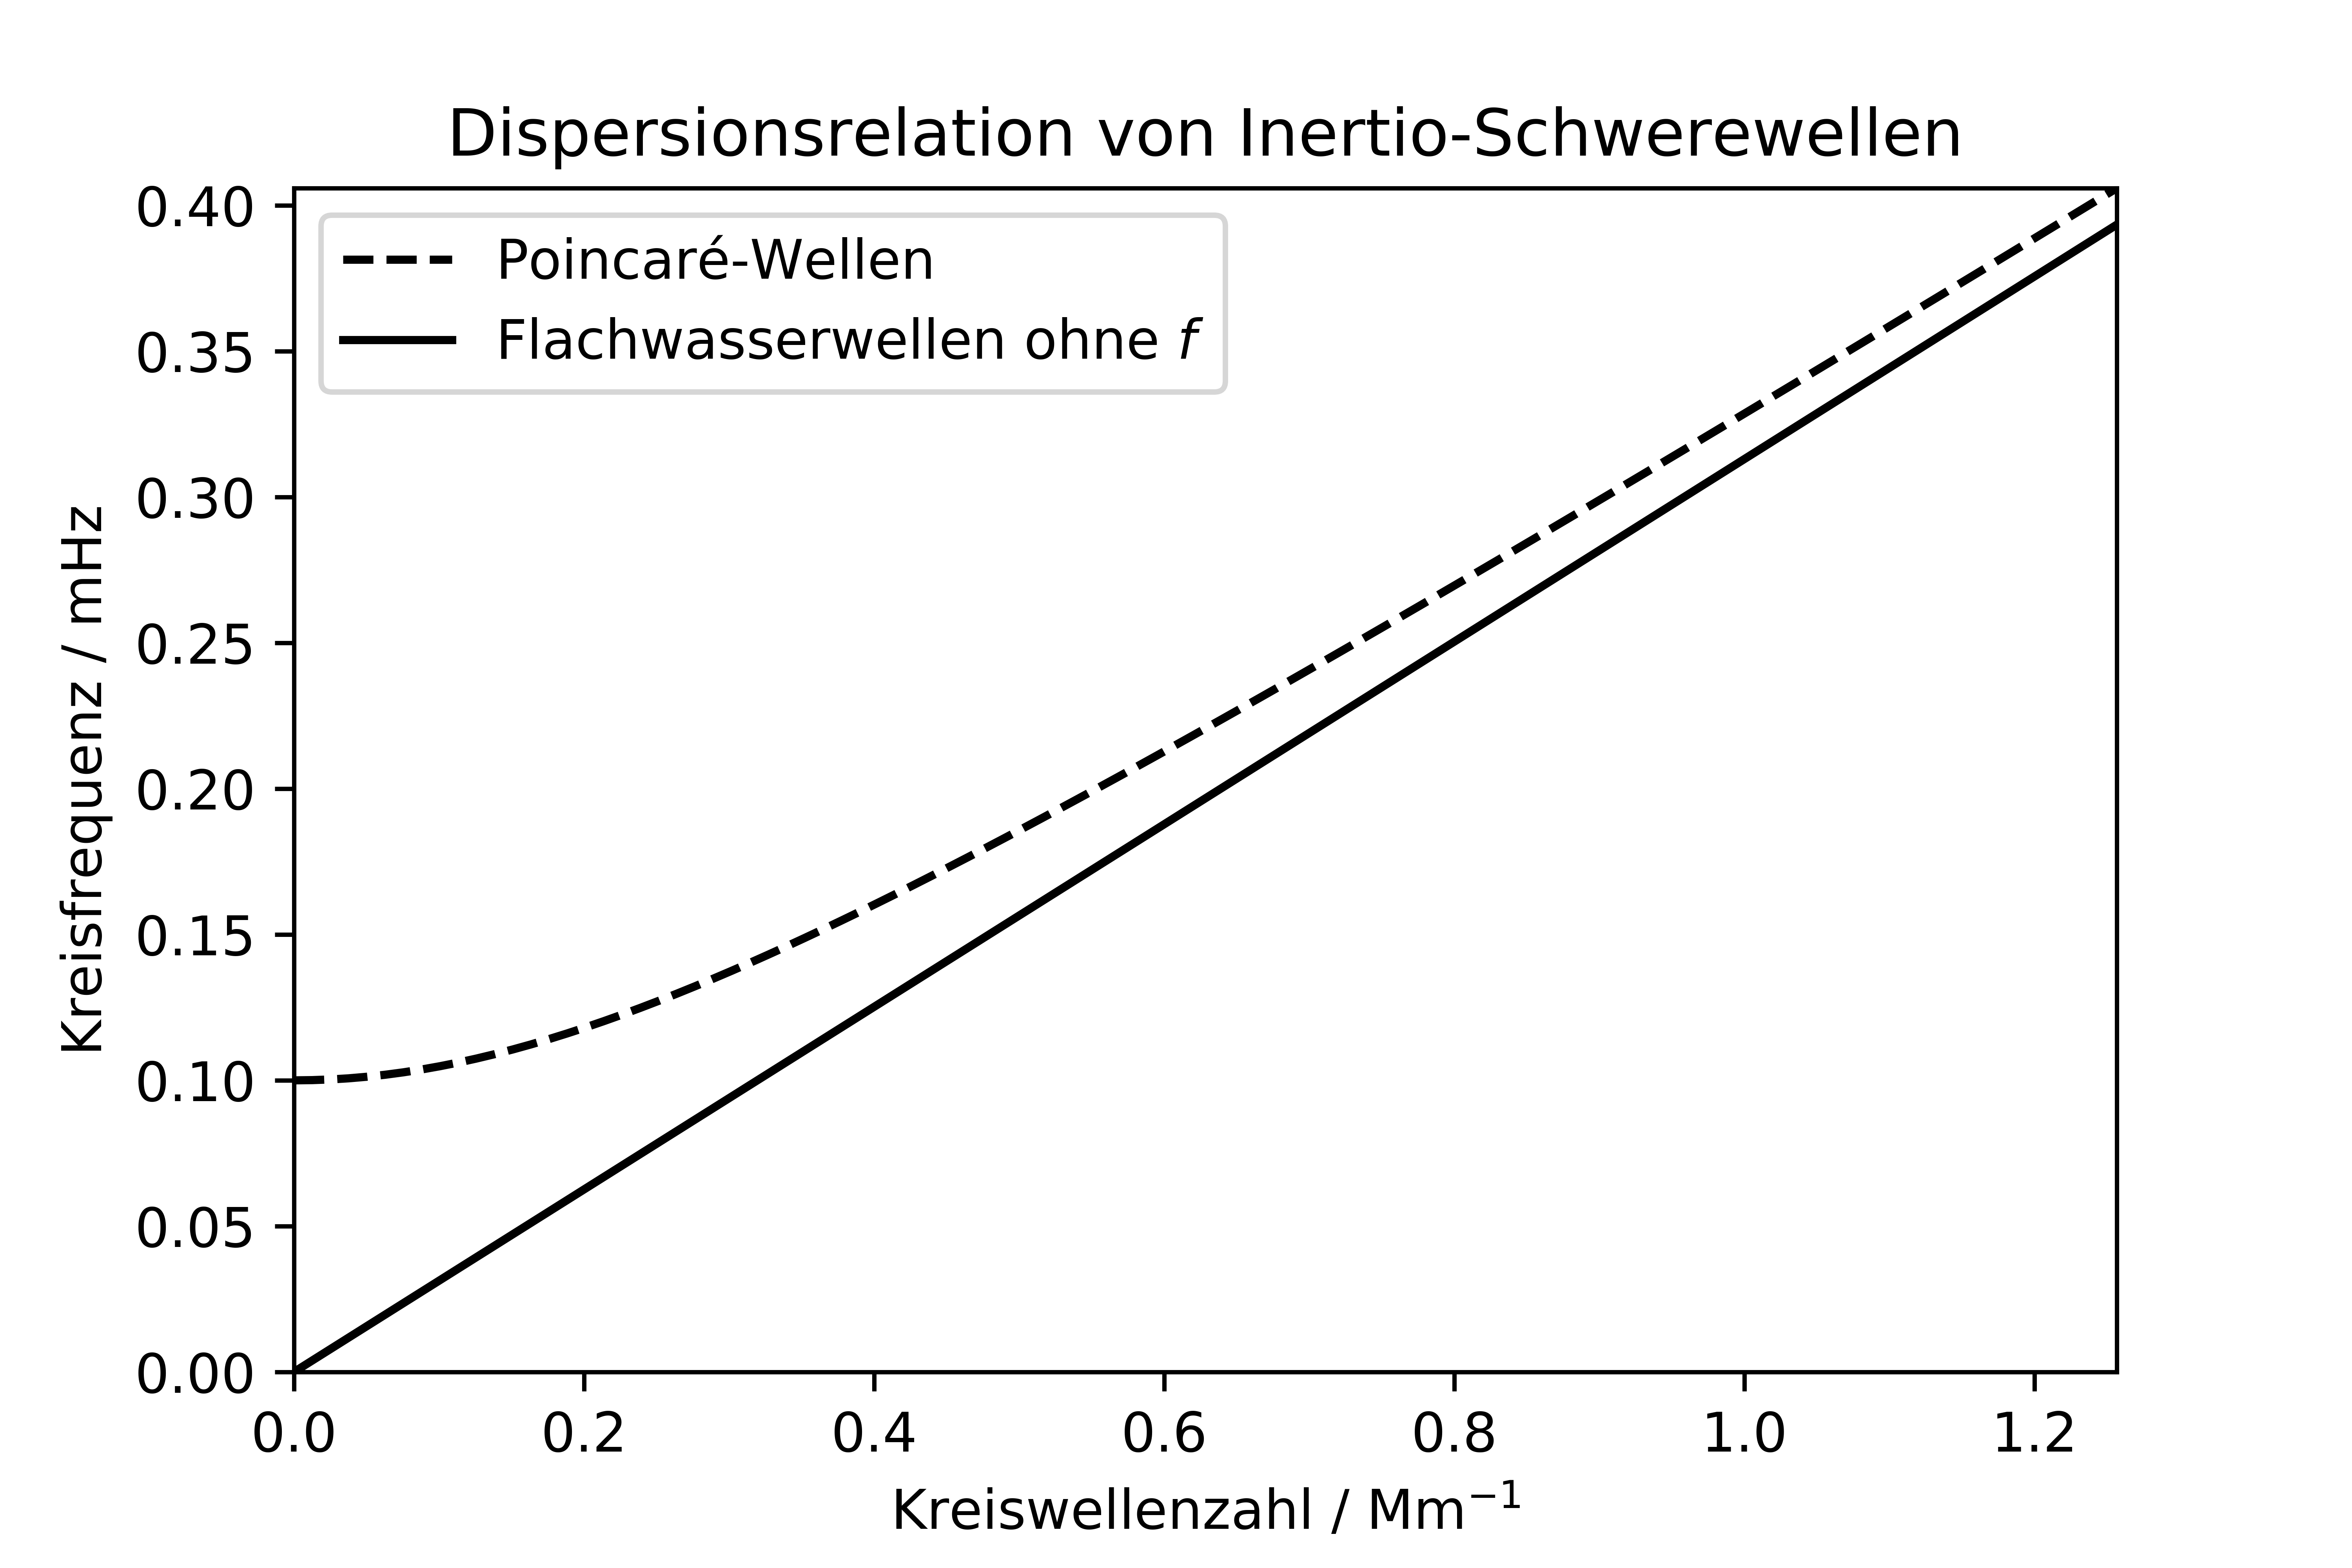
\includegraphics[width = 0.6\textwidth]{figs/inertio_gravity_dispersion.png}
\caption{Die Dispersionsrelation von Poincaré-Wellen im Vergleich zur Dispersion von Flachwasserwellen ohne Coriolis-Beschleunigung. Es wurde mit $f = 10^{-4}$ 1/s und $H = 10$ km gerechnet.}
\label{fig:poincare_dispersion}
\end{center}
\end{figure}
%
\begin{align}
c^2 = \frac{\omega^2}{k^2} = gH + \frac{f^2}{k^2} = gH + f^2L^2\frac{1}{4\pi^2}
\end{align}
%
mit $L$ als Wellenlänge. Die Poincaré-Wellen haben also eine höhere Phasengeschwindigkeit als die Schwerewellen ohne Erdrotation. Desto kürzer die Wellen werden, desto geringer wird der Einfluss der Coriolis-Kraft, für lange Wellen jedoch geht $\omega$ gegen $f$. Der Ausdruck für $c^2$ der Poincaré-Wellen ist gegenüber dem der Schwerewellen ohne Coriolis-Kraft um den Ausdruck $f^2L^2\frac{1}{4\pi^2}$ höher. Um eine Grenzwellenlänge $R_o$ zu bestimmen, ab der die Wirkung der Coriolis-Kraft deutlich wird, setzt man
%
\begin{align}
f_0^2R_o^2\frac{1}{4\pi^2} = \frac{gH}{4\pi^2}\approx 0, 025gH.
\end{align}
%
Daraus erhält man für den barotropen Rossby-Radius
%
\begin{align}
R_o = \frac{\sqrt{gH}}{\left|f\right|}.\label{eq:def_baro_ro_r}
\end{align}
%
Setzt man typische Werte ein, folgt $R_o \approx2000$ km.

\subsection{Kapillarwellen}
\label{sec:kapillarwellen}\index{Kapillarwelle}

Im Fall $\eta = \hat{\eta}\exp\left(ikx - i\omega t\right)$ folgt
%
\begin{align}
-\frac{1}{\rho}\frac{\partial p_k}{\partial x} & = -\frac{k^2\sigma}{\rho}\frac{\partial\eta}{\partial x}.
\end{align}
%
Addiert man dies zur rechten Seite von Glg. $\eqref{eq:deep_1}$, erhält man
%
\begin{align}
-g\frac{\partial\eta}{\partial x} &\to -g\frac{\partial\eta}{\partial x} - \frac{\sigma k^2}{\rho}\frac{\partial\eta}{\partial x} = -g\left(1 + \frac{k^2\sigma}{\rho g}\right)\frac{\partial\eta}{\partial x}, 
\end{align}
%
Man muss also
%
\begin{align}
g \to g\left(1 + \frac{k^2\sigma}{\rho g}\right)
\end{align}
%
ersetzen, der Rest der Herleitung überträgt sich. Man erhält also die Dispersionsrelation der Kapillarwellen
%
\begin{align}
\omega^2 = kg\left(1 + \frac{k^2\sigma}{\rho g}\right)\tanh\left(kD\right).
\end{align}
%
Im Fall sehr kurzer Wellen erhält man den Grenzfall
%
\begin{align}
\omega^2 & = \frac{k^3\sigma}{\rho} \Rightarrow c = \sqrt{\frac{2\pi\sigma}{\rho\lambda}}.
\end{align}
%
In diesem Grenzfall sind Kapillarwellen also anormal dispergiert.

Um eine Grenzwällenlänge $\lambda_K$ herzuleiten, ab der kapillare Effekte wichtig werden, rechnet man
%
\begin{align}
\frac{k_K^2\sigma}{\rho g} \stackrel{!}{\geq} \frac{1}{10} \Leftrightarrow \lambda_K \leq \sqrt{\frac{40\pi^2\sigma}{\rho g}}.
\end{align}
%
Die Oberflächensapnnung von Wasser beträgt ca. $\sigma \sim 75$ mN/m, woraus folgt
%
\begin{align}
\lambda_K \sim 5,5\text{ cm}.
\end{align}

\subsection{Inertialwellen}
\label{sec:inertialwellen}\index{Inertialwelle}

Bei Inertialwellen\index{Inertialwellen} geht man von einem verschwindenden horizontalen Druckgradienten aus, sodass nur die Coriolis-Kraft übrigbleibt. Die Impulsgleichungen der SWEs Glg. \eqref{eq:swe_0} werden unter Vernachlässigung der advektiven Terme zu
%
\begin{align}
\frac{d u}{dt} = f_0v, && \frac{d v}{dt} = -f_0u.
\end{align}
%
Für den Coriolis-Parameter wird dabei ein ortsunabhängiger Wert $f_0$ verwendet, um den $\beta-$Effekt zu umgehen. Man macht einen Ansatz
%
\begin{align}
u = U\exp\left(-i\omega t\right), && v = V\exp\left(-i\omega t\right)
\end{align}
%
mit eventuell komplexen Amplituden $U, V$. Setzt man dies in das Gleichungssystem ein, erhält man
%
\begin{align}
-i\omega U = f_0V, && -i\omega V = -f_0 U.
\end{align}
%
Als Matrixgleichung wird dies zu
%
\begin{align}
\left(\begin{array}{cc}
- i\omega& -f_0\\
f_0& -i\omega
\end{array}\right)\left(\begin{array}{c}
U\\
V
\end{array}\right) = \mathbf{0}.
\end{align}
%
Nichttriviale Lösungen existieren für
%
\begin{align}
- \omega^2 + f_0^2 & = 0, 
\end{align}
%
also für
%
\begin{align}
\omega = \pm f.
\end{align}
%
Die Teilchen bewegen sich also auf einer Kreisbahn mit Radius
%
\begin{align}
R_I = \frac{V}{f_0}.
\end{align}
%
Setzt man eine Geschwindigkeit von $1$ $\frac{\text{m}}{\text{s}}$ ein, so folgt beispielsweise $R_I = 10$ km mit $f_0 = 10^{-4}\:\text{s}^{-1}$. Für die Periode gilt
%
\begin{align}
T = \frac{2\pi}{f_0} \approx \frac{1\:\text{d}}{2\sin\left(\varphi\right)}, 
\end{align}
%
d = $24$ h ist die Dauer eines Tages. Typische Inertialperioden liegen also im Größenordnungsbereich von einem Tag.

Da die totalen Ableitungen $\md{}$ verwendet wurden, wurde implizit eine Trajektorie ausgerechnet. Diese Trajektorie ist eine Kreisbahn, jedoch nur unter Annahme eines ortsunabhängigen Coriolis-Parameters. Im Allgemeinen sind die Teilchentrajektorien jedoch aufgrund des $\beta-$Effektes keine geschlossenen Kreisbahnen. Ebenso wurde \underline{kein} Windfeld $\mathbf{v}_h\left(\mathbf{r}, t\right)$ bestimmt.

\subsection{Kelvin-Wellen}
\label{sec:kelvin-wellen}\index{Kelvin-Welle}

Man geht wieder aus vom Gleichungssystem der Glg.en \eqref{eq:dyn_in_grav_1} - \eqref{eq:dyn_in_grav_3}, diesmal stellt man sich jedoch die Halbebene $x<0$ als Küste vor, sodass nur die verbleibende Halbebene $x\geq 0$ vom Fluid beströmt werden kann. Die Randbedingung lautet also
%
\begin{align}
u\left(x = 0\right) = 0.
\end{align}
%
Gesucht wird nun nach Lösungen, die dies global erfüllen. Hierzu geht man wieder von der f-Ebene aus. Das Gleichungssystem reduziert sich auf
%
\begin{align}
0 & = -g\frac{\partial\eta}{\partial x} + fv, \label{eq:kelvin_1}\\
\frac{\partial v}{\partial t} & = -g\frac{\partial\eta}{\partial y}, \label{eq:kelvin_2}\\
\frac{\partial\eta}{\partial t} + H \frac{\partial v}{\partial y} & = 0.\label{eq:kelvin_3}
\end{align}
%
Aus Glg. \eqref{eq:kelvin_1} folgt, dass $v$ geostrophisch balanciert ist, sodass man $v$ aus den verbleibenden beiden Gleichungen eliminieren kann:
%
\begin{align}
\frac{\partial^2\eta}{\partial t\partial x} & = -f\frac{\partial\eta}{\partial y},\\
\frac{\partial\eta}{\partial t} + H\frac{g}{f}\frac{\partial^2\eta}{\partial x\partial y} & = 0.
\end{align}
%
Hier macht man den harmonischen Wellenansatz
%
\begin{align}
\eta = \eta_0\exp\left[i\left(k_xx + k_yy - \omega t\right)\right], 
\end{align}
%
woraus folgt
%
\begin{align}
-iwik_x & = -fik_y\Rightarrow wk_x = -ifk_y, \label{eq:kelvin_deriv_1}\\
-i\omega + H\frac{g}{f}ik_xik_y & = 0 \Rightarrow i\omega = -H\frac{g}{f}k_xk_y.\label{eq:kelvin_deriv_2}
\end{align}
%
Aus Glg. \eqref{eq:kelvin_deriv_1} folgt
%
\begin{align}
k_x = -\frac{i}{\omega}fk_y, 
\end{align}
%
was in Glg. \eqref{eq:kelvin_deriv_2} eingesetzt
%
\begin{align}
i\omega & = -H\frac{g}{f}k_y\left(-\frac{i}{\omega}fk_y\right) = iH\frac{g}{\omega}k_y^2
\end{align}
%
ergibt. Definiert man $\kappa$ durch
%
\begin{align}
\kappa \coloneqq \frac{\omega}{\sqrt{gH}} > 0
\end{align}
%
mit einer als positiv angenommenen Kreisfrequenz $\omega > 0$, folgt
%
\begin{align}
k_y = \pm\kappa.\label{eq:kelvin_deriv_3}
\end{align}
%
Dies ergibt umgeformt
%
\begin{align}
\omega = \pm k_y\sqrt{gH}.
\end{align}
%
Mit Glg. \eqref{eq:kelvin_deriv_1} folgt
%
\begin{align}
k_x = \mp if\frac{1}{\sqrt{gH}}.
\end{align}
%
$\eta$ darf als Funktion des Abstands von der Küste nicht exponentiell ansteigen, daher gilt bei $f > 0$ das negative Vorzeichen in Glg. \eqref{eq:kelvin_deriv_3}, bei $f < 0$ das positive. Auf der Nordhalbkugel hat die Kelvin-Welle die Küste also rechts von der Ausbreitungsrichtung, auf der Südhalbkugel links.

Die Penetrationslängen $l$ der Kelvin-Wellen ergeben sich zu
%
\begin{align}
l = l\left(f, H\right) = \frac{2\pi\sqrt{gH}}{\left|f\right|} = 2\pi R_o
\end{align}
%
mit dem in Glg. \eqref{eq:def_baro_ro_r} definierten Rossby-Radius $R_o$.

\begin{figure}
\centering
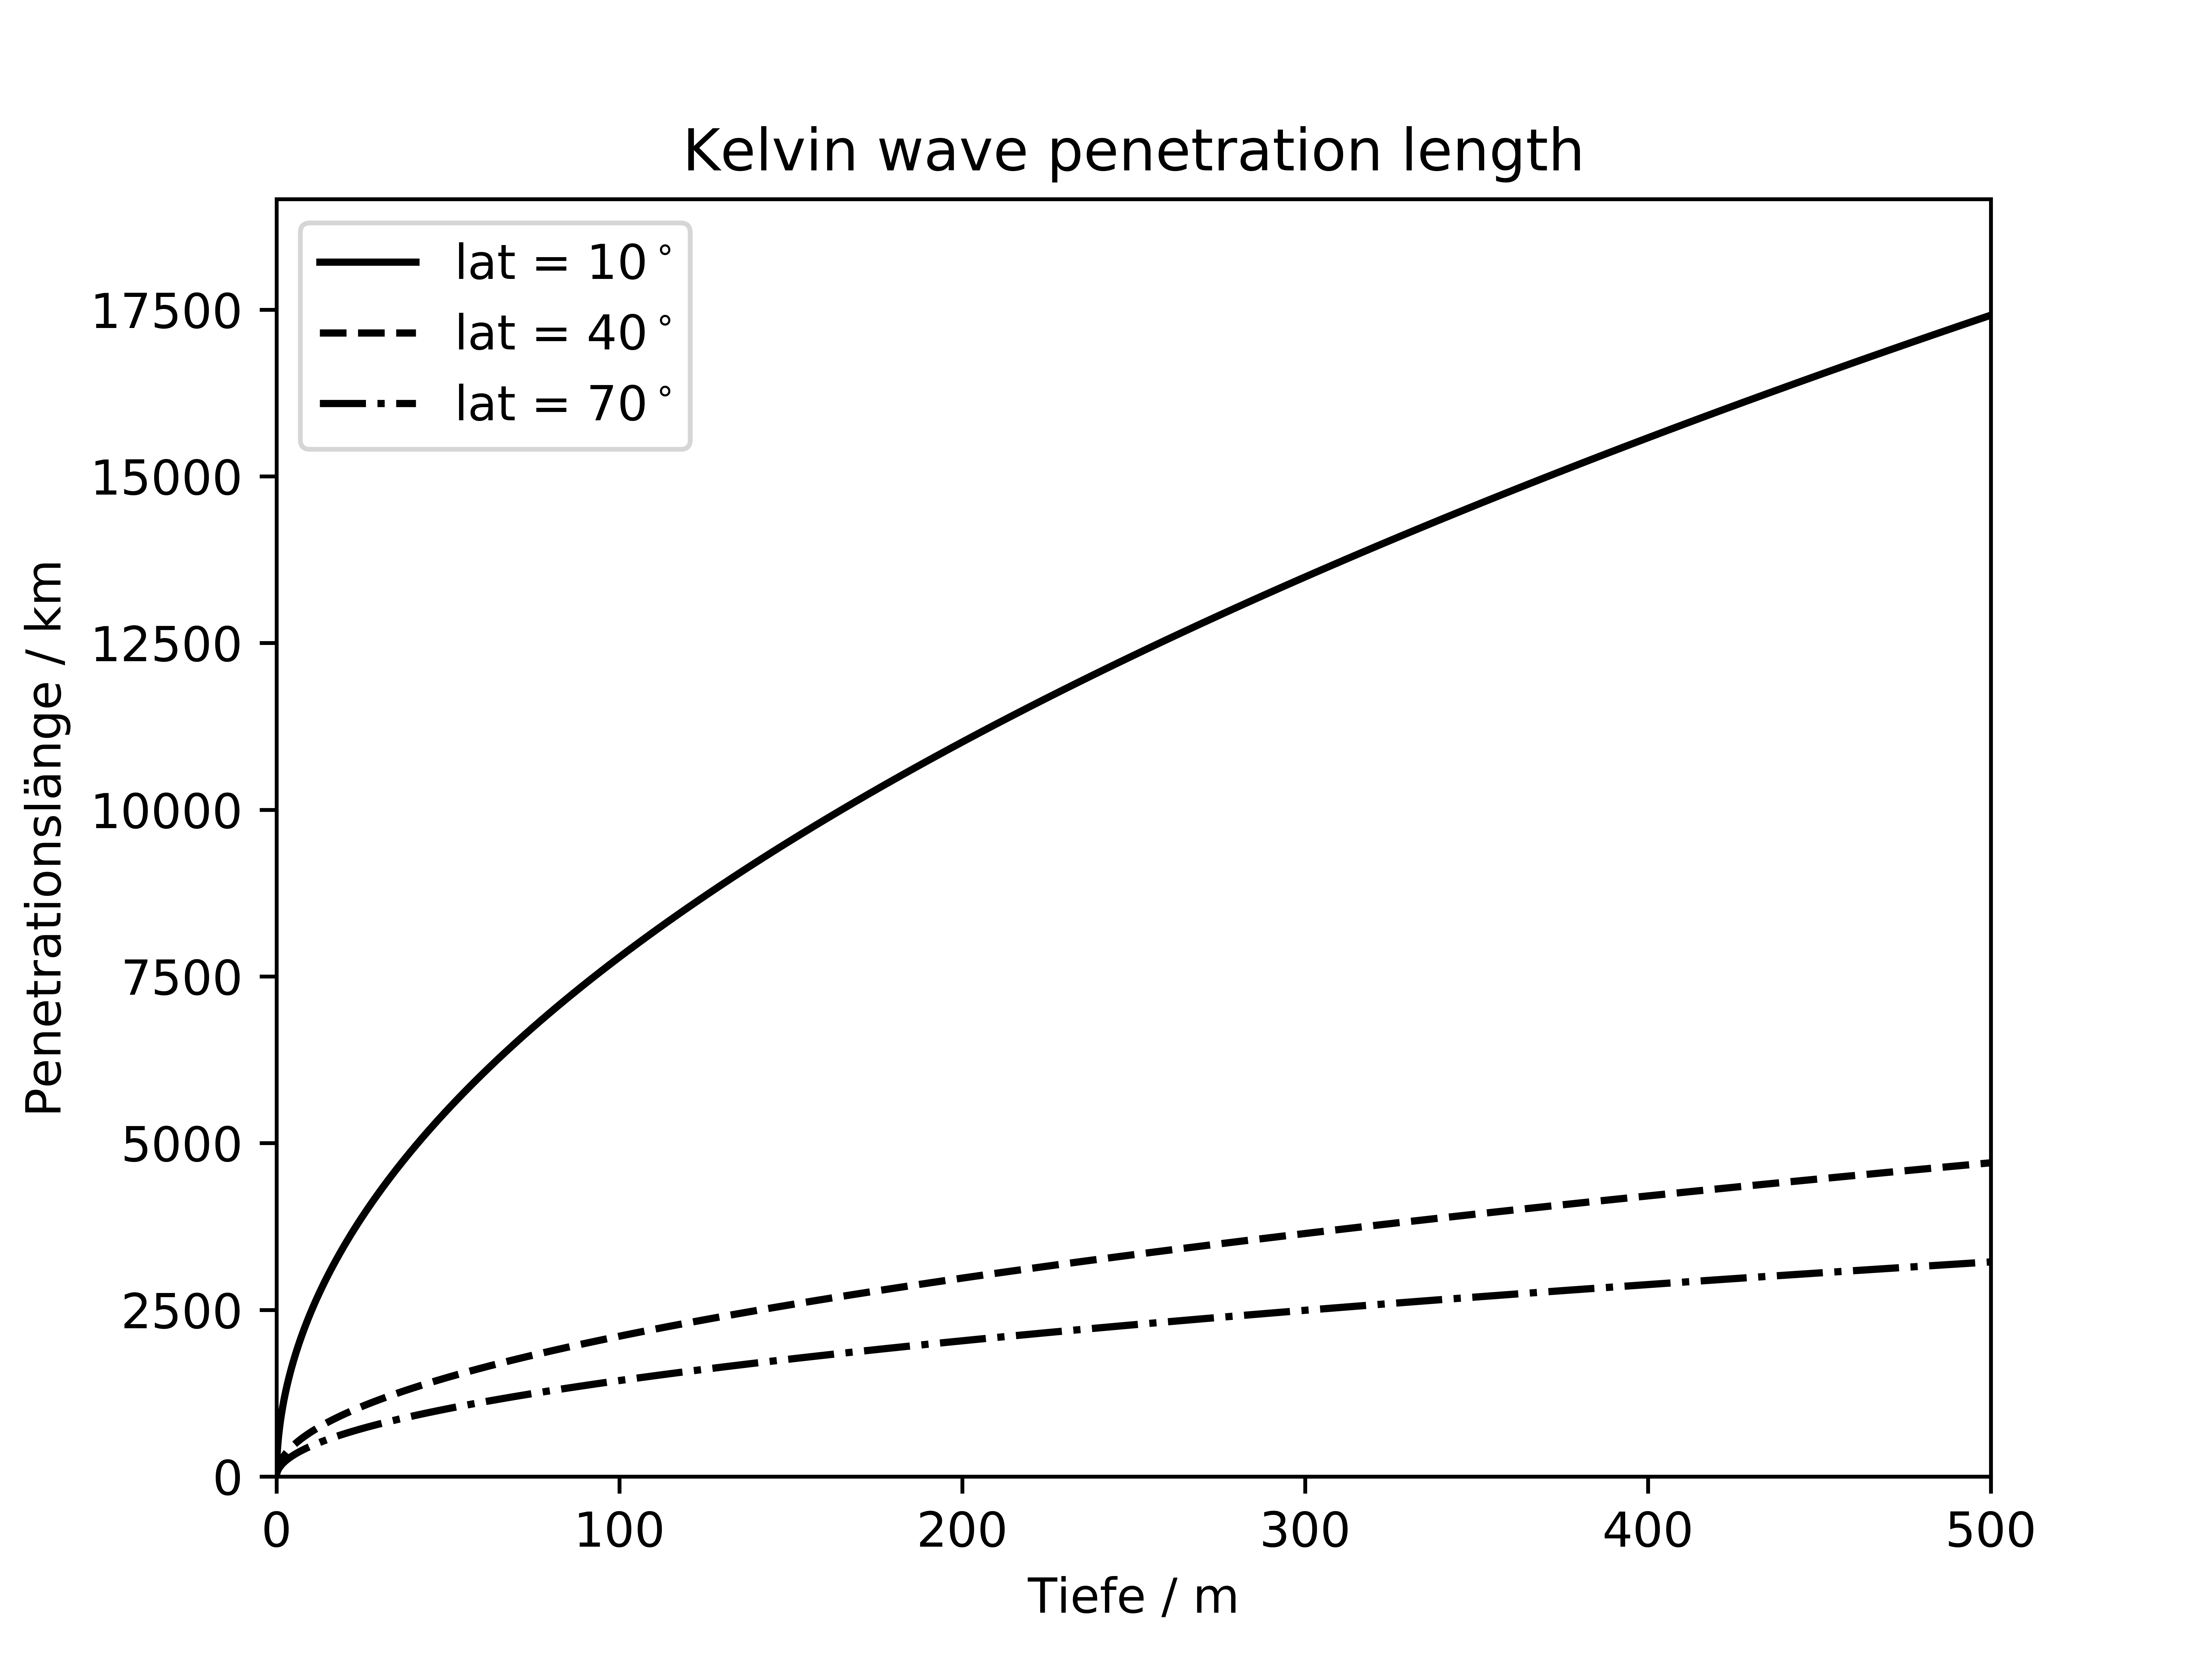
\includegraphics[width = .6\textwidth]{figs/kelvin_pen.png}
\caption{Penetrationslängen der Kelvin-Wellen.}
\label{fig:kelvin_pen}
\end{figure}

Abb. \ref{fig:kelvin_pen} zeigt die typischen Penetrationslängen von Kelvin-Wellen, diese liegen schnell im Bereich von $1000$ - $10000$ km, also durchaus im Bereich von zehn bis mehreren hundert Prozent eines Viertels des Erdumfangs. Diese Ausdehnung übersteigt die Gültigkeit der f-Ebene bei weitem.

\subsection{Äquatoriale Kelvin-Wellen}
\label{sec:aequatoriale_kelvin-wellen}\index{Kelvin-Welle!äquatoriale}\index{äquatoriale Kelvin-Welle}

Am Äquator kann man nicht $f = f_0$ setzen, man setzt stattdessen die $\beta-$Ebene
%
\begin{align}
f = \beta y
\end{align}
%
mit
%
\begin{align}
\beta \coloneqq \frac{\partial f}{\partial y}\newvline_{\varphi = 0}
\end{align}
%
an. Damit lauten die Glg.en \eqref{eq:dyn_in_grav_1} - \eqref{eq:dyn_in_grav_3}
%
\begin{align}
\frac{\partial u}{\partial t} & = -g\frac{\partial\eta}{\partial x} + \beta yv,\\
\frac{\partial v}{\partial t} & = -g\frac{\partial\eta}{\partial y} - \beta yu,\\
\frac{\partial\eta}{\partial t} + H\left(\frac{\partial u}{\partial x} + \frac{\partial v}{\partial y}\right) & = 0.
\end{align}
%
Nun sucht man nach Lösungen mit $v = 0$. In diesem Fall gilt
%
\begin{align}
\frac{\partial u}{\partial t} & = -g\frac{\partial\eta}{\partial x},\\
0 & = -g\frac{\partial\eta}{\partial y} - \beta yu,\\
\frac{\partial\eta}{\partial t} + H\frac{\partial u}{\partial x} & = 0.
\end{align}
%
Über
%
\begin{align}
u = -\frac{g}{\beta y}\frac{\partial\eta}{\partial y}
\end{align}
%
lässt sich $u$ eliminieren:
%
\begin{align}
-\frac{g}{\beta y}\frac{\partial^2\eta}{\partial t\partial y} & = -g\frac{\partial\eta}{\partial x}\\
\frac{\partial\eta}{\partial t} - \frac{gH}{\beta y}\frac{\partial^2\eta}{\partial x\partial y} & = 0
\end{align}
%
Der Ansatz
%
\begin{align}
\eta = \newhat{\eta}\exp\left[i\left(k_xx + k_yy -\omega t\right)\right]
\end{align}
%
führt auf
%
\begin{align}
-\frac{g}{\beta y}k_y\omega & = -gik_x \Rightarrow k_y = \frac{1}{\omega}\beta yik_x,\\
-i\omega + \frac{gH}{\beta y}k_xk_y & = 0 \Rightarrow \omega^2 = gHk_x^2.
\end{align}
%
Es gilt also
%
\begin{align}
k_x = \pm\frac{\omega}{\sqrt{gH}}.
\end{align}
%
Für $k_y$ folgt
%
\begin{align}
k_y = \frac{1}{\omega}\beta yik_x = \pm i\frac{\beta y}{\sqrt{gH}}.
\end{align}
%
Nur das Pluszeichen kommt in Frage. Die Lösung lautet also
%
\begin{align}
\eta = \newhat{\eta}\exp\left[i\left(k_xx + i\frac{\beta y^2}{\sqrt{gH}} - \sqrt{gH}k_xt\right)\right].
\end{align}
%
Um die meridionale Ausdehnung $y_0$ dieser Wellen abzuschätzen, setzt man
%
\begin{align}
1 = \frac{2\omega y_0^2}{\sqrt{gH}}
\end{align}
%
an. Hieraus folgt
%
\begin{align}
y_0 =\sqrt{R\frac{\sqrt{gH}}{2\omega}} = 2071\text{ km}
\end{align}
%
mit $R$ als Äquatorradius und $H = 1$ km.

\subsection{Globale Moden}
\label{sec:globale_moden}\index{globale Mode}

Nimmt man eine \text{f-Kugel}\index{f-Kugel} an, also eine Kugel mit homogenem Coriolis-Parameter $f$ (dies ist ein rein mathematisches Konzept), haben die linearisierten SWEs Glg.en \eqref{eq:flach_lin_1} - \eqref{eq:flach_lin_2} globale analytische Lösungen. Zunächst rechnet man
%
\begin{align}
\frac{\partial^2d}{\partial t^2} & = -D\nabla\cdot\frac{\partial\mathbf{v}_h}{\partial t}.
\end{align}
%
Bildet man die Divergenz von Glg. \eqref{eq:flach_lin_1}, folgt mit Glg. \eqref{eq:diff_op_rule_9}
%
\begin{align}
\nabla\cdot\frac{\partial\mathbf{v}_h}{\partial t} & = f\zeta - g\Delta d\Rightarrow\frac{\partial^2d}{\partial t^2} = -D\left(f\zeta - g\Delta d\right)\nonumber\\
\Rightarrow\frac{\partial^3d}{\partial t^3}& = -D\left[f\frac{\partial\zeta}{\partial t} - g\Delta\frac{\partial d}{\partial t}\right].
\end{align}
%
Mit Glg. \eqref{eq:vorticit_z_baro_swes_pre} folgt näherungsweise
%
\begin{align}
\frac{\partial\zeta}{\partial t} & = \frac{f}{D}\frac{\partial d}{\partial t}\Rightarrow\frac{\partial^3 d}{\partial t^3} = -f^2\frac{\partial d}{\partial t} + Dg\Delta\frac{\partial d}{\partial t}.
\end{align}
%
Man macht den Ansatz
%
\begin{align}
d = Y_{l, m}e^{-i\omega t}
\end{align}
%
mit einer Kugelflächenfunktion $Y_{l, m}$. Somit folgt
%
\begin{align}
i\omega^3d & = f^2i\omega d + i\omega\frac{gD}{a^2}l\left(l + 1\right)d\nonumber\\
\Rightarrow\omega\left(\omega^2 - f^2 - l\left(l + 1\right)\frac{gD}{a^2}\right) & = 0.\label{eq:disprel_global_modes}
\end{align}
%
Für die Kreisfrequenzen gilt $\omega_0 = 0$ und
%
\begin{align}
\omega_l = \pm\sqrt{f^2 + l\left(l + 1\right)\frac{gD}{a^2}}
\end{align}
%
bzw. für die Periodendauern $T_0 = \infty$ und
%
\begin{align}
T_l = \frac{2\pi}{\sqrt{f^2 + l\left(l + 1\right)\frac{gD}{a^2}}}.
\end{align}
%
\renewcommand{\arraystretch}{1.2}
\begin{table}
\centering
\begin{tabular}{|c|c|}
\hline \textbf{Wellenzahl $l$} & \textbf{Periodendauer / hr} \\
\hline\hline
1 & 14, 8 \\
\hline 
2 & 11, 8 \\
\hline 
3 & 9, 5 \\
\hline 
4 & 7, 8 \\
\hline 
5 & 6, 6 \\
\hline 
\end{tabular}
\caption{Periodendauern der gloablen Moden für $D = 8$ km und $f = 10^{-4}$ s$^{-1}$.}
\label{tab:perioden_glob}
\end{table}
\renewcommand{\arraystretch}{1.0}
%
Tab. \ref{tab:perioden_glob} gibt eine Vorstellung von den Periodendauern.

\subsection{Rossby-Wellen}
\label{sec:rossbywellen}\index{barotrope Rossby-Welle}\index{Rossby-Welle!barotrope}

Im vorigen Abschnitt \ref{sec:poincare-wellen} wurde von $\beta = 0$ ausgegangen. In diesem Fall sind die dort hergeleiteten Poincaré-Wellen die allgemeinsten Wellenlösungen. Eine neue Art der Wellen entsteht, wenn man die Breitenabhängigkeit von $f$ berücksichtigt.

Man geht aus von einem homogenen zonalen Grundstrom $U$. Man nimmt $u_0 = 0$ an, außerdem geht man von $k_y = 0$ aus, die Störungen sollen nur x-abhängig sein. Man weiß schon jetzt:
%
\begin{itemize}
\item Da $U$ homogen ist und $u_0 = 0$, $v = v\left(x, t\right)$ gelten, sind die Lösungen divergenzfrei.
\end{itemize}
%
Daher kann man die barotrope Vorticitygleichung verwenden. Macht man den Ansatz
%
\begin{align}
v = v_0\exp\left[i\left(kx - \omega t\right)\right]
\end{align}
%
dann gelten
%
\begin{align}
\zeta = ikv, && \frac{\partial\zeta}{\partial t} = k\omega v, && \frac{\partial\zeta}{\partial x} = -k^2v.
\end{align}
%
Setzt man dies in die barotrope Vorticitygleichung ein, erhält man
%
\begin{align}
k\omega v_0 & = Uk^2v_0 - v_0\beta\Leftrightarrow\omega = Uk - \frac{\beta}{k}.\label{eq:rossby_welle_barotrop_disp}
\end{align}
%
Glg. \eqref{eq:rossby_welle_barotrop_disp} ist die Dispersionsrelation der Rossby-Wellen. Für ihre Phasengeschwindigkeit gilt
%
\begin{align}
c = U - \frac{\beta}{k^2}.
\end{align}
%
Im hypothetischen Fall $U\to0$, $L = 2\pi a$ und $\varphi = 0$ gilt
%
\begin{align}
\left|c\right| = 2\omega\frac{1}{a}\frac{4\pi^2 a^2}{4\pi^2} = 2\omega a = 930\:\frac{\text{m}}{\text{s}}.
\end{align}
%
Dies ist eine betragsmäßige Beschränkung von $c$. Keine Welle kann sich schneller fortpflanzen als mit der Geschwindigkeit $2\omega a$, und schneller kann das System der herrschenden Gleichungen keine Information übertragen.

\subsubsection{Anschauliches Verständnis}
\label{sec:anschauliches_verstaendnis}

\begin{figure}
\centering
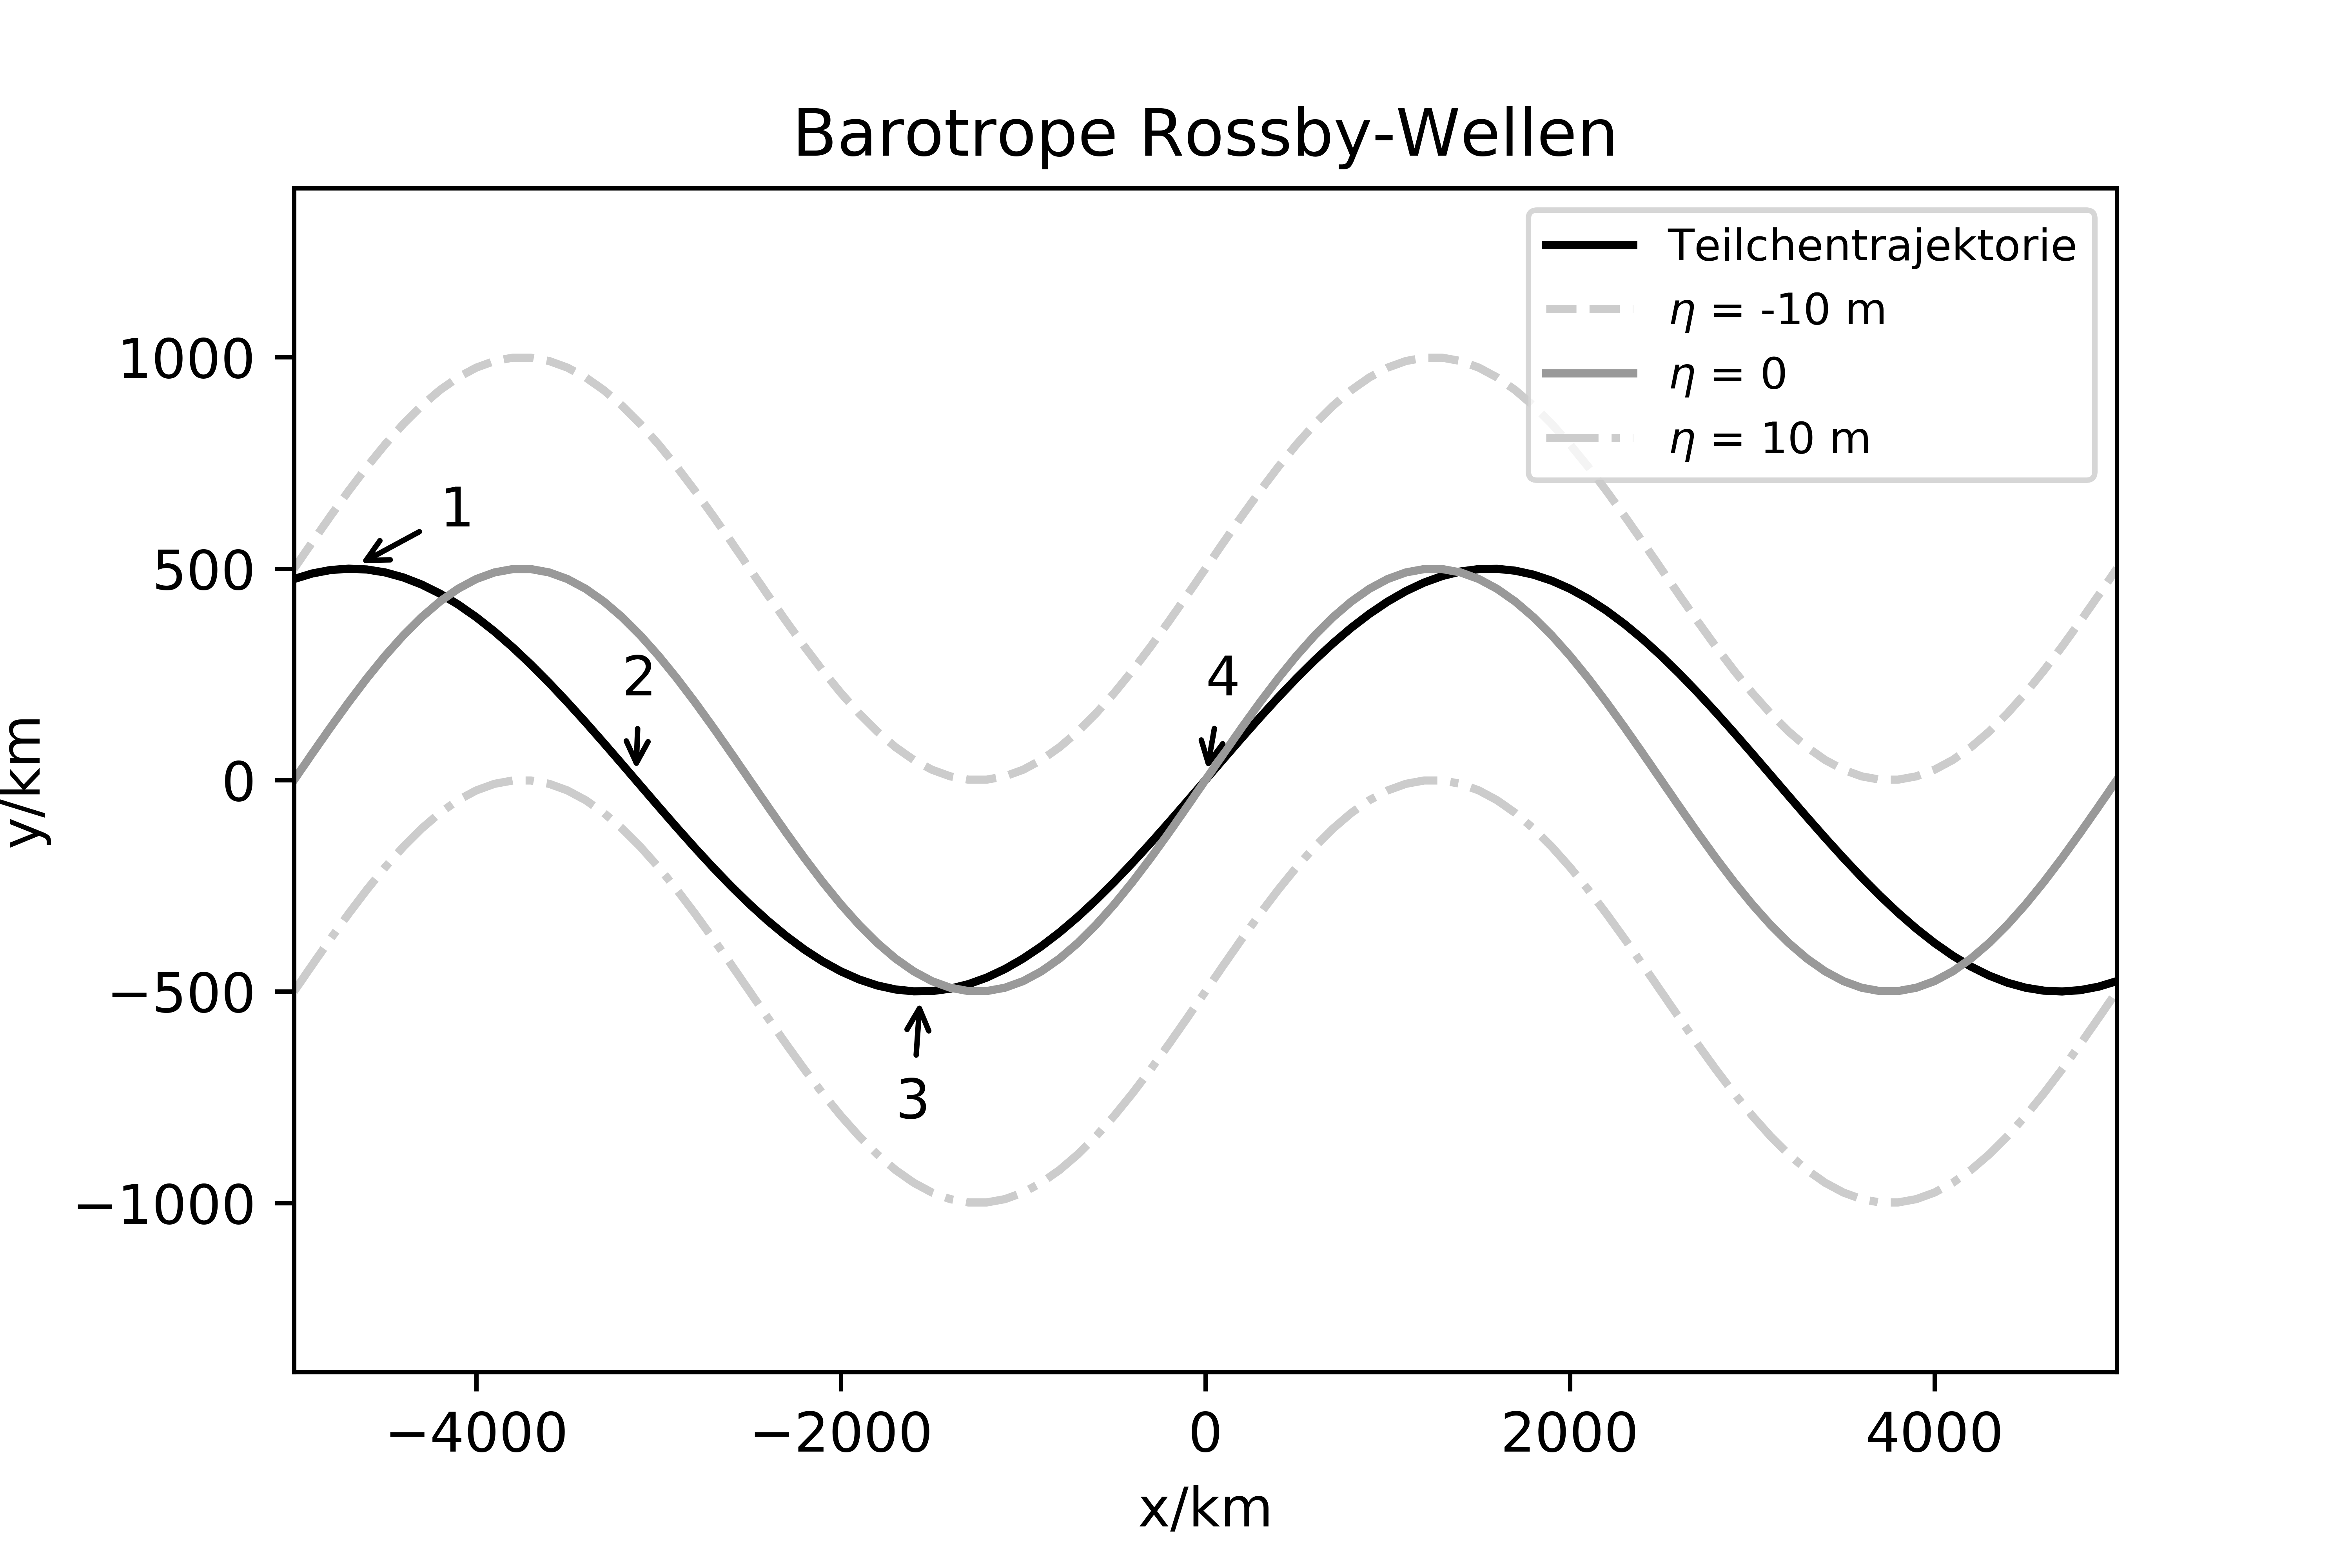
\includegraphics[width = .6\textwidth]{figs/rossby_waves_vorticity.png}
\caption{Veranschaulichung des Prinzips der Erhaltung der absoluten Vorticity. 1: $f$ maximal, $\zeta$ minimal, 2: $f = f_0$, $\zeta = 0$, 3: $f$ minimal, $\zeta$ maximal, 4: $f = f_0$, $\zeta = 0$. Man beachte auch, dass die Wellenlänge der Teilchentrajektorie größer ist, als die der Welle.}
\label{fig:rossby_wellen_barotrop}
\end{figure}

Die y-Komponente der Impulsgleichung im Flachwassermodell lautet
%
\begin{align}
\md{v} = -fu - g\frac{\partial\eta}{\partial y}.\label{eq:momentum_swe_y}
\end{align}
%
Mache für $f$ eine lineare Taylor-Entwicklung
%
\begin{align}
f = f_0 + \beta y.
\end{align}
%
Ein homogener zonaler Grundstrom $U$ kann geostrophisch balanciert werden durch eine Oberflächenauslenkung
%
\begin{align}
0 = -f_0U - g\frac{\partial\eta}{\partial y}.
\end{align}
%
In diesem Fall wird Glg. \eqref{eq:momentum_swe_y} zu
%
\begin{align}
\md{^2y}{t^2} = -\beta U y.
\end{align}
%
Dies entspricht einem harmonischen Oszillator mit der Eigenfrequenz
%
\begin{align}
\omega_{\text{ind}} = \sqrt{\beta U}.
\end{align}
%
Daher muss $U>0$ westlich sein. Die Eigenfrequenz wurde mit einem Index $\text{ind}$ gekennzeichnet, da es sich um die individuelle Schwingungsfrequenz der Teilchen und nicht um die Frequenz $\omega$ der Welle handelt.

Eine weitere anschauliche Erklärung ergibt sich aus der barotropen Vorticitygleichung, diese lautet
%
\begin{align}
f + \zeta = \text{const}.
\end{align}
%
Wird ein Teilchen von seiner Ruhelage auf der Nordhalbkugel bei vorhandenem westlichen Grundstrom nach Norden ausgelenkt, so nimmt $f$ zu. Daher muss $\zeta$ abnehmen und das Teilchen erhält antizyklonale relative Vorticity. Anschließend schwingt es über seine Ruhelage hinaus nach Süden, wobei $f$ abnimmt. Daher erhält das Teilchen zyklonale relative Vorticity und schwenkt wieder nach Norden. Der Mechanismus der barotropen Rossby-Wellen ist also die Erhaltung der absoluten Vorticity, s. auch Abb. \ref{fig:rossby_wellen_barotrop}.

Barotrope Rossby-Wellen sind trotz der umfassenden Vereinfachungen (Barotropie und Divergenzfreiheit) in der Atmosphäre und im Ozean relevant. In der Atmosphäre sind sie aufgrund ihrer Divergenzfreiheit am ehesten auf die mittlere Troposphäre anwendbar, sie liefern eine einfache Betrachtung des meandernden Polarjets. Hierbei wird häufig der Begriff der Wellenzahl verwendet, eine Welle der Wellenzahl $n$ hat eine zonale räumliche Periode von $\frac{2\pi}{n}$ als Winkel. Rossby-Wellen breiten sich im Ozean aufgrund des geringen östlichen (nach Osten gerichteten) Grundstroms immer nach Westen aus (es ist $\beta\geq0$ auf der gesamten Erde).

\section{Barokline Wellen}
\label{sec:barokline_wellen}\index{barokline Welle}\index{Welle!barokline}

\subsection{Schichtungswellen}
\label{sec:schichtungswellen}\index{Schichtungswelle}

Diese Wellen entstehen im kontinuierlichen, hydrostatischen, thermisch stabilen Medium bei vertikaler Auslenkung eines Teilchens. Von einer kontinuierlichen Schichtung spricht man, falls die Dichte eine kontinuierliche (stetig-differenzierbare) Funktion der Vertikalkoordinate ist: $\rho = \rho (z)$. Ein Teilchen der Dichte $\rho _0 = \rho (z_0)$ habe seine Ruhelage in der Höhe $z_0$, die hier o. B. d. A. zu $z_0 = 0$ festgelegt sei. Lenkt man das Teilchen vertikal aus, lautet die Bewegungsgleichung
%
\begin{align}
\frac{d^2z}{dt^2} = -\frac{1}{\rho_0}\frac{\partial p}{\partial z} - g = g\frac{\rho}{\rho_0} - g = \frac{g}{\rho_0}\left(\rho - \rho_0\right), \label{eq:momentum_schichtung}
\end{align}
%
$z(t)$ sei die Auslenkung. Hierbei wurde angenommen, dass das Teilchen seine Dichte während der Auslenkung nicht ändert. Nähert man die Abweichung $\rho (z) - \rho _0$ mittels einer Taylor-Entwicklung zu
%
\begin{align}
\rho (z) - \rho_0 = \frac{\partial\rho}{\partial z}(z = 0)z, 
\end{align}
%
so folgt für die Schwingungsgleichung
%
\begin{align}
\frac{d^2z}{dt^2}(t) = \frac{g}{\rho_0}\frac{\partial\rho}{\partial z}z(t)\label{eq:schichtungs_dg}.
\end{align}
%
Setzt man $z = Z_1\exp\left(iNt\right) + Z_2\exp\left(-iNt\right)$ an, so folgt für die Kreisfrequenz
%
\begin{align}
N^2 = -\frac{g}{\rho}\frac{\partial\rho}{\partial z}, 
\end{align}
%
$N$ ist die \textit{Brunt-Väisälä-Frequenz}\index{Brunt-Väisälä-Frequenz}, sie ist ein Maß für die Stabilität. Setzt man $N$ in \eqref{eq:schichtungs_dg} ein, erhält man
%
\begin{align}
\frac{d^2z}{dt^2} = -N^2z.
\end{align}
%
Hieran sieht man, dass im Fall $N^2 > 0$ eine Sinusschwingung als Lösung folgt, während im Fall $N^2 < 0$ eine reelle Exponentialfunktion die Lösung ist, da das Teilchen von seinem Ursprungsort wegbeschleunigt wird. Im Fall $N^2> 0$ ist die Schichtung also stabil, während sie im Fall $N^2<0$ labil ist. Eine stabile Schichtung bezeichnet man auch als starke Schichtung. Im Fall $N^2 = 0$ ist die Schichtung neutral.

Die obige Herleitung ist noch nicht ganz vollständig, da Inkompressibilität angenommen wurde. Streng genommen bleibt bei der Auslenkung nicht die Dichte, sondern die potentielle Dichte bezogen auf das Referenzniveau erhalten. Bezeichnet $\newtilde{\rho}(z)$ die Dichte des Teilchens bei einer Auslenkung $z$, so wird damit Gleichung \eqref{eq:momentum_schichtung} zu
%
\begin{align}
\frac{d^2z}{dt^2} = \frac{1}{\newtilde{\rho}\left(z\right)}g\rho\left(z\right) - g = \frac{g}{\newtilde{\rho}\left(z\right)} \left(\rho\left(z\right) - \newtilde{\rho}\left(z\right)\right).
\end{align}
%
Der Ausdruck $\rho\left(z\right) - \newtilde{\rho}\left(z\right)$ ist die Dichtedifferenz zwischen dem umgebenden Fluid und dem betrachteten Teilchen. Bringt man beide Systeme nun adiabatisch auf $z = 0$, so gilt nach Glg. \eqref{eq:pot_dichte} für ihre Dichtedifferenz
%
\begin{align}
\Delta\rho = \left(\rho\left(z\right) - \newtilde{\rho}\left(z\right)\right)\left(\frac{p_0}{p}\right)^{1/\kappa}.
\end{align}
%
Hierbei sind $p \coloneqq p\left(z\right)$ und $p_0 \coloneqq p\left(0\right)$. In erster Ordnung ist $p = p_0$, $\Delta\rho$ ist dann die Differenz der potentiellen Dichten in Bezug aufs Referenzniveau $z = 0$. Deshalb kann man auch die potentiellen Dichten $\rho _\theta$ (bezogen auf $z = 0$) einsetzen. Man erhält in erster Ordnung
%
\begin{align}
\frac{d^2z}{dt^2} = \frac{g}{\newtilde{\rho}(z)}\left(\rho_\theta(z) - \rho_\theta(0)\right) = \frac{g}{\newtilde{\rho}(z)}\frac{\partial\rho_\theta}{\partial z}z.
\end{align}
%
Für die Brunt-Väisälä-Frequenz folgt
%
\begin{center}
\doublebox{\parbox{0.8\textwidth}{
\begin{center}
\begin{align}
N^2 = -\frac{g}{\rho_\theta}\frac{\partial\rho_\theta}{\partial z}.\label{eq:brunt_v_frequency_prop_0}
\end{align}
\end{center}
}}
\end{center}
%
Dies ist der allgemeine Ausdruck für die Brunt-Väisälä-Frequenz in einem kompressiblen Medium. $N^2$ ist ein Feld, was von allen drei Koordinaten und der Zeit abhängen kann. Die potentielle Dichte muss dabei immer auf das Niveau bezogen werden, auf dem man sich befindet. In einer trockenen Atmosphäre kann man $N^2$ auch über die potentielle Temperatur $\theta$ ausdrücken:
%
\begin{align}
\rho_\theta = \frac{p_0}{R_d\theta}
\end{align}
%
Somit folgt
%
\begin{align}
\frac{\partial\rho_\theta}{\partial z} = -\frac{p_0}{R_d\theta^2}\frac{\partial\theta}{\partial z}.
\end{align}
%
Für die Brunt-Väisälä-Frequenz bedeutet dies
%
\begin{align}
N^2 & = \frac{g}{\theta}\frac{\partial\theta}{\partial z}.\label{eq:bv_freq_theta}
\end{align}
%
Schichtungswellen entstehen zum Beispielen als Leewellen hinter Orographie, in diesem Fall ergeben sich sinusförmige Trajektorien $(ut, z_0\sin\left(Nt\right))^T$. Wird dabei Sättigung erreicht, entstehen in den Wellenbergen Oszillationswolken.
%
\subsection{Vertikale Moden}
\label{sec:vertikale_moden}\index{vertikale Mode}

Hier geht man von einem ebenen Untergrund in der Tiefe $z = -D < 0$ aus und fordert die Randbedingungen
%
\begin{align}
w\left(z = 0\right) & = 0,\\
w\left(z = -D\right) & = 0.
\end{align}
%
Man verwendet folgendes Gleichungssystem, wobei man o. B. d. A. von einer in x-Richtung propagierenden Welle ausgeht:
%
\begin{align}
\frac{\partial u}{\partial t} & = -\frac{1}{\rho_0}\frac{\partial p'}{\partial x},\\
\frac{\partial w}{\partial t} & = -\frac{1}{\rho_0}\frac{\partial p'}{\partial z},\\
\frac{\partial\rho'}{\partial t} & = -\rho_0\frac{\partial u}{\partial x} - \rho_0\frac{\partial w}{\partial z}.
\end{align}
%
Hierbei ist
%
\begin{align}
\rho = \rho_0 + \rho'
\end{align}
%
mit einer homogenen Hintergrunddichte $\rho_0$ und einer Fluktuation $\rho'$. Analog zerlegt man den Druck $p$, wobei gelten soll
%
\begin{align}
\frac{\partial p_0}{\partial z} = -g\rho_0.
\end{align}
%
Man macht nun die Ansätze
%
\begin{align}
u = U\left(z\right)\exp\left(ikx-i\omega t\right), && v = V\left(z\right)\exp\left(ikx-i\omega t\right),\\
p' = P\left(z\right)\exp\left(ikx-i\omega t\right), && \rho' = \newtilde{\rho}\left(z\right)\exp\left(ikx-i\omega t\right).
\end{align}
%
Setzt man dies in des geltende Gleichungssystem ein, folgt
%
\begin{align}
-i\omega U = -\frac{ikP}{\rho_0} \Rightarrow \omega U & = \frac{kP}{\rho_0}, \label{eq:v_mode_deriv_2}\\
-i\omega W = -\frac{P'}{\rho_0} \Rightarrow \omega W & = -i\frac{P'}{\rho_0}, \label{eq:v_mode_deriv_1}\\
-i\omega\newtilde{\rho} = -\rho_0ikU - \rho_0W' \Rightarrow \omega\newtilde{\rho} & = \rho_0kU - i\rho_0W'.
\end{align}
%
Die dritte Gleichung ist immer erfüllbar, $\newtilde{\rho}\left(z\right)$ kann entsprechend gewählt werden. Für $W$ macht man den Ansatz
%
\begin{align}
W\left(z\right) = \newhat{w}\sin\left(n\pi\frac{z}{D}\right)
\end{align}
%
mit $n\geq 1$. Aus Glg. \eqref{eq:v_mode_deriv_1} folgt
%
\begin{align}
P' = \rho_0i \omega\newhat{w}\sin\left(n\pi\frac{z}{D}\right).
\end{align}
%
Für $P$ setzt man daher
%
\begin{align}
P\left(z\right) = -\frac{D\rho_0i\omega\newhat{w}}{n\pi}\cos\left(n\pi\frac{z}{D}\right)
\end{align}
%
an. Setzt man dies in Glg. \eqref{eq:v_mode_deriv_1} folgt
%
\begin{align}
U\left(z\right) = \frac{kP}{\omega\rho_0} = -\frac{ki\newhat{w}D}{n\pi}\cos\left(n\pi\frac{z}{D}\right).
\end{align}
%
Es gilt also
%
\begin{align}
u\left(x, z, t\right) & = \frac{Dk\newhat{w}}{n\pi}\cos\left(n\pi\frac{z}{D}\right)\exp\left[i\left(kx - \omega t - \frac{\pi}{2}\right)\right]\nonumber\\
\Rightarrow\Re\left(u\left(x, z, t\right)\right) & = \frac{Dk\newhat{w}}{n\pi}\cos\left(n\pi\frac{z}{D}\right)\sin\left(kx - \omega t\right).
\end{align}
%
Dier Horizontaldivergenz $\delta$ an der Oberfläche ergibt sich zu
%
\begin{align}
\delta\left(z = 0\right) = \frac{\partial\Re\left(u\left(x, z, t\right)\right)}{\partial x} = \frac{Dk^2\newhat{w}}{n\pi}\cos\left(n\pi\frac{z}{D}\right)\cos\left(kx - \omega t\right).
\end{align}
%
Vertikale Moden führen also an der Oberfläche zu alternierenden Streifen von Divergenz und Konvergenz. Im Bereich der Konvergenz werden die Oberflächenwellen horizontal komprimiert, was das Wellenfeld destabilisiert, andersherum wird das Wellenfeld im Bereich der Divergenz stabilisiert, wozu auch beiträgt, dass in diesem Bereich das Wasser aus der Tiefe an die Oberfläche kommt und dieses Wasser noch keiner Windeinwirkung ausgesetzt war.

\subsection{Barokline Rossby-Wellen}
\label{sec:barokline_rossbywellen}\index{Rossby-Welle!barokline}\index{barokline Rossby-Welle}
%
Hier geht man aus vom hydrostatischen adiabatischen Gleichungssystem.
%
\begin{align}
\md{_h\mathbf{v}_h} + \omega\frac{\partial\mathbf{v}_h}{\partial p}&\stackrel{\text{Glg.en }\eqref{eq:x_momentum_simplified_simplified_p}\text {, }\eqref{eq:y_momentum_simplified_simplified_p}}{=} -f\mathbf{k}\times\mathbf{v}_h - \nabla\phi, \label{eq:hydrostat_1}\\
\frac{\partial\phi}{\partial p}&\stackrel{\text{Glg. }\eqref{eq:hydrostatic_p}}{=} -\alpha, \label{eq:hydrostat_2}\\
\md{_hT} - S_p\omega&\stackrel{\text{Glg. }\eqref{eq:td1_ideal_gas_p}}{=} 0, \label{eq:hydrostat_3}\\
\nabla\cdot\mathbf{v}_h + \frac{\partial\omega}{\partial p}&\stackrel{\text{Glg. }\eqref{eq:kont_p}}{=} 0, \label{eq:hydrostat_4}\\
p\alpha&\stackrel{\text{Glg. }\eqref{eq:zustand_ideal_alt}}{=} R_dT.\label{eq:hydrostat_5}
\end{align}
%
Nun müssen zunächst einige Vereinfachungen vorgenommen werden. Ziel ist das \textit{quasigeostrophische Gleichungssystem}.\index{Quasigeostrophie} Dieses Konzept wendet man ausschließlich auf Kanäle in den Extratropen an, die schmal genug für die $\beta-$Ebene sind. Setzt man Glg. \eqref{eq:hydrostat_5} in Glg. \eqref{eq:hydrostat_2} ein, folgt
%
\begin{align}
\frac{\partial\phi}{\partial p} = -\frac{R_dT}{p}\Rightarrow T = -\frac{p}{R_d}\frac{\partial\phi}{\partial p}.
\end{align}
%
Dies setzt man nun in Glg. \eqref{eq:hydrostat_3} ein, es folgt
%
\begin{align}
\md{_h}\left(\frac{\partial\phi}{\partial p}\right) + \frac{R_dS_p}{p}\omega = 0.
\end{align}
%
Man definiert nun den \textit{statischen Stabilitätsparameter}\index{Stabilitätsparameter!statischer}\index{statischer Stabilitätsparameter} $\sigma$ durch
%
\begin{align}
\sigma \coloneqq\frac{R_dS_p}{p}\stackrel{\text{Glg. }\eqref{eq:stabilitaetspara_vereinfacht}}{=} - \frac{R_dT}{p}\frac{1}{\theta}\frac{\partial\theta}{\partial p} = -\frac{\alpha}{\theta}\frac{\partial\theta}{\partial p}.
\end{align}
%
Dies hängt nach Glg. \eqref{eq:bv_freq_theta} über
%
\begin{align}
\sigma = -\frac{\alpha}{\theta}\frac{\partial z}{\partial p}\frac{\partial\theta}{\partial z} = \frac{\alpha^2}{g\theta}\frac{\partial\theta}{\partial z} = \frac{\alpha^2}{g^2}\frac{g}{\theta}\frac{\partial\theta}{\partial z} = \left(\frac{\alpha}{g}N\right)^2
\end{align}
%
mit der Brunt-Väisälä-Frequenz $N$ zusammen. Man nähert außerdem den Coriolis-Parameter $f$ zu
%
\begin{align}
f = f_0 + \beta\left(y - y_0\right)\stackrel{y_0 \equiv 0}{=}f_0 + \beta y, 
\end{align}
%
vgl. Absch. \ref{sec:entwicklungen_des_coriolisparameters_in_ebener_geometrie}. Dann gilt für den geostrophischen Wind Glg. \eqref{eq:geostr_wind}
%
\begin{align}
\mathbf{v}_{h, g} = \mathbf{k}\times\frac{1}{f}\nabla\phi = \mathbf{k}\times\frac{1}{f_0}\nabla\phi - \mathbf{k}\times\frac{\beta y}{f_0^2}\nabla\phi + \mathcal{O}\left(f''\right)\stackrel{\text{in 0. Ordnung}}{\to}\mathbf{v}_{h, g} = \mathbf{k}\times\frac{1}{f_0}\nabla\phi.\label{eq:geostr_wind_vereinfacht}
\end{align}
%
Hieraus kann man für den thermischen Wind ableiten
%
\begin{align}
\frac{\partial\mathbf{v}_{h, g}}{\partial p} = -\frac{1}{f_0}\mathbf{k}\times\nabla\alpha.
\end{align}
%
Die relative Vorticity $\zeta$ ersetzt man nun näherungsweise durch die relative Vorticity des geostrophischen Windes $\zeta_g$, welche nach Glg. \eqref{eq:geostro_vort_skal} näherungsweise durch
%
\begin{align}
\zeta_g = \frac{1}{f_0}\Delta\phi.
\end{align}
%
gegeben ist. Für die absolute Vorticity nähert man hieraus folgernd
%
\begin{align}
\eta_g \coloneqq f + \zeta_g = f_0 + \beta y + \zeta_g.
\end{align}
%
Mit Glg. \eqref{eq:geostr_wind_vereinfacht} vereinfacht man nun die materielle Ableitung zu
%
\begin{align}
\md{} & = \md{_h} + \omega\frac{\partial}{\partial p} = \frac{\partial}{\partial t} + \mathbf{v}_h\cdot\nabla_h + \omega\frac{\partial}{\partial p}\nonumber\\
&\to \md{^{(g)}} \coloneqq\md{_h^{(g)}} + \omega\frac{\partial}{\partial p} = \frac{\partial}{\partial t} + \mathbf{v}_{h, g}\cdot\nabla_h + \omega\frac{\partial}{\partial p}.
\end{align}
%
Hiermit folgt für den Ersten Hauptsatz
%
\begin{align}
\frac{\partial}{\partial t}\left(\frac{\partial\phi}{\partial p}\right) = -\mathbf{v}_{h, g}\cdot\nabla_h\left(\frac{\partial\phi}{\partial p}\right) - \sigma\omega.\label{eq:first_theorem_qg}
\end{align}
%
Die Vorticitygleichung Glg. \eqref{eq:vorticity_p} wird hier noch einmal wiederholt:
%
\begin{align}
\frac{\partial\zeta}{\partial t} & = -v\beta - \left(f + \zeta\right)\nabla\cdot\mathbf{v}_h - \mathbf{v}_h\cdot\nabla\zeta - \omega\frac{\partial\zeta}{\partial p} + \mathbf{k}\cdot\left[\frac{\partial\mathbf{v}_h}{\partial p}\times\nabla\omega\right]
\end{align}
%
Der geostrophische Wind ist nach Absch. \ref{sec:geostrophie} eine Größenordnung größer als die ageostrophische Komponente, daher kann man die horizontale Advektion mit $\mathbf{v}_{h, g}$ berechnen und $\zeta$ durch $\zeta_g$ ersetzen:
%
\begin{align}
\frac{\partial\zeta_g}{\partial t} & = -v_g\beta - \left(f + \zeta_g\right)\nabla\cdot\mathbf{v}_h - \mathbf{v}_{h, g}\cdot\nabla\zeta_g - \omega\frac{\partial\zeta_g}{\partial p} + \mathbf{k}\cdot\left[\frac{\partial\mathbf{v}_{h}}{\partial p}\times\nabla\omega\right]
\end{align}
%
Die Werte in Tab. \ref{tab:syn_scale} ergeben außerdem in SI-Einheiten
%
\begin{itemize}
\item $\frac{\partial\zeta_g}{\partial t}\sim10^{-10}$, 
\item $\omega\frac{\partial\zeta_g}{\partial p}\sim10^{-11}$, 
\item $\mathbf{k}\cdot\left[\frac{\partial\mathbf{v}_h}{\partial p}\times\nabla\omega\right]\sim10^{-11}$.
\end{itemize}
%
Folglich können auch der Drehterm und die vertikale Advektion vernachlässigt werden und außerdem die relative gegenüber der absoluten Vorticity im Drehterm, dies führt mit $f\approx f_0$ auf die sogenannte \textit{quasigeostrophische Vorticitygleichung}\index{Vorticitygleichung!quasigeostrophische}\index{quasigeostrophische Vorticitygleichung}
%
\begin{align}
\frac{\partial\zeta_g}{\partial t} & = -\mathbf{v}_{h, g}\cdot\nabla\left(\zeta_g + f\right) - f_0\nabla\cdot\mathbf{v}_h = -\mathbf{v}_{h, g}\cdot\nabla\left(\zeta_g + f\right) + f_0\frac{\partial\omega}{\partial p}.\label{eq:vorticity_p_qg}
\end{align}
%
An dieser Stelle führt man zur Vereinfachung eine Stromfunktion
%
\begin{align}
\psi \coloneqq\frac{\phi}{f_0}
\end{align}
%
ein, damit folgen
%
\begin{align}
\mathbf{v}_{h, g} & = \mathbf{k}\times\nabla\psi, \label{eq:geostr_wind_stream}\\
\zeta_g & = \Delta_h\psi.
\end{align}
%
Hieraus folgt für die Vorticitygleichung Glg. \eqref{eq:vorticity_p_qg} und den Ersten Hauptsatz Glg. \eqref{eq:e_vom_pot}
%
\begin{align}
\Delta\frac{\partial\psi}{\partial t} & = -\mathbf{v}_{h, g}\cdot\nabla\left(\Delta\psi + f\right) + f_0\frac{\partial\omega}{\partial p}, \label{eq:vorticity_p_qg_mod}\\
\frac{\partial}{\partial t}\left(\frac{\partial\psi}{\partial p}\right) & = -\mathbf{v}_{h, g}\cdot\nabla\left(\frac{\partial\psi}{\partial p}\right) - \frac{\sigma}{f_0}\omega\nonumber\\
\Rightarrow\frac{f_0^2}{\sigma}\frac{\partial^2}{\partial p^2}\left(\frac{\partial\psi}{\partial t}\right) & = -\frac{f_0^2}{\sigma}\mathbf{v}_h\cdot\nabla\left(\frac{\partial^2\psi}{\partial p^2}\right) - f_0\frac{\partial\omega}{\partial p}
\end{align}
%
Bei der letzten Implikation wurde die $p-$Abhängigkeit von $\sigma$ vernachlässigt und dies wird auch weiterhin getan werden. Da $\sigma$ mit der Schichtung zusammenhängt, ist dies eine schlechte Annahme, da die Schichtung natürlich in der Realität innerhalb der Troposphäre stark ortsabhängig ist. Nichtsdestotrotz kann man diese Annahme hier machen, da die relevanten Phänomene durch diese Annahme nicht gefiltert werden. Außerdem wurde
%
\begin{align}
\frac{\partial\mathbf{v}_{h, g}}{\partial p}\cdot\nabla\left(\frac{\partial\psi}{\partial p}\right) \stackrel{\text{Glg. \eqref{eq:geostr_wind_stream}}}{=}\left(\mathbf{k}\times\nabla\frac{\partial\psi}{\partial p}\right)\cdot\nabla\left(\frac{\partial\psi}{\partial p}\right) = 0
\end{align}
%
eingesetzt. Nun werden die beiden Gleichungen addiert
%
\begin{align}
\frac{\partial}{\partial t}\left[f + \Delta\psi + \frac{f_0^2}{\sigma}\frac{\partial^2\psi}{\partial p^2}\right] + \mathbf{v}_{h, g}\cdot\nabla\left(f + \Delta\psi + \frac{f_0^2}{\sigma}\frac{\partial^2\psi}{\partial p^2}\right) = 0.\label{eq:tendency_eq_pre}
\end{align}
%
Die Größe
%
\begin{align}
q_g \coloneqq f + \Delta\psi + \frac{f_0^2}{\sigma}\frac{\partial^2\psi}{\partial p^2}
\end{align}
%
bezeichnet man als \textit{quasigeostrophische potentielle Vorticity}, \index{Vorticity!quasigeostrophische!potentielle}\index{quasigeostrophische potentielle Vorticity} damit lässt sich Glg. \eqref{eq:tendency_eq_pre} als
%
\begin{center}
\doublebox{\parbox{0.8\textwidth}{
\begin{center}
\begin{align}
\md{_h^{(g)}}q_g = 0\label{eq:tendency_eq}
\end{align}
\end{center}
}}
\end{center}
%
notieren. Dies ist die sogenannte \index{Tendenzgleichung}\textit{Tendenzgleichung}. $\omega$ kann hieraus diagnostiziert werden, hierzu wendet man zunächst den horizontalen Laplace-Operator $\Delta_h$ auf Glg. \eqref{eq:first_theorem_qg} an:
%
\begin{align}
\Delta\frac{\partial}{\partial p}\frac{\partial\psi}{\partial t} = -\Delta_h\left[\mathbf{v}_{h, g}\cdot\nabla\left(\frac{\partial\psi}{\partial p}\right)\right] - \frac{\sigma}{f_0}\Delta\omega.\label{eq:omega_eq_deriv_1}
\end{align}
%
Nun wird Glg. \eqref{eq:vorticity_p_qg} nach $p$ differenziert:
%
\begin{align}
\frac{\partial}{\partial p}\Delta\frac{\partial\psi}{\partial t} = -\frac{\partial}{\partial p}\left[\mathbf{v}_{h, g}\cdot\nabla\left(\Delta\psi + f\right)\right] + f_0\frac{\partial^2\omega}{\partial p^2}\label{eq:omega_eq_deriv_2}
\end{align}
%
Nun subtrahiert man Glg. \eqref{eq:omega_eq_deriv_1} von \eqref{eq:omega_eq_deriv_2} und erhält
%
\begin{align}
0 & = \Delta\left[\mathbf{v}_{h, g}\cdot\nabla\left(\frac{\partial\psi}{\partial p}\right)\right] + \frac{\sigma}{f_0}\Delta\omega - \frac{\partial}{\partial p}\left[\mathbf{v}_{h, g}\cdot\nabla\left(\Delta\psi + f\right)\right] + f_0\frac{\partial^2\omega}{\partial p^2}\nonumber
\end{align}
\begin{center}

\doublebox{\parbox{0.8\textwidth}{
\begin{center}
\begin{align}
\Rightarrow\left[\Delta + \frac{f_0^2}{\sigma}\frac{\partial^2}{\partial p^2}\right]\omega & = \frac{f_0}{\sigma}\frac{\partial}{\partial p}\left[\mathbf{v}_{h, g}\cdot\nabla\left(\Delta\psi + f\right)\right] + \frac{f_0}{\sigma}\Delta\left[\mathbf{v}_{h, g}\cdot\nabla\left(\frac{\partial\psi}{\partial p}\right)\right].\label{eq:omega_eq}
\end{align}
\end{center}
}}
\end{center}
%
Dies ist die \textit{$\omega-$Gleichung}\index{$\omega-$Gleichung}. Dieser Formalismus ist aufgrund der darin enthaltenen linearen Entwicklung von $f$ nicht global anwendbar, die Leistungsfähigkeit besteht darin, dass hiermit innerhalb zonaler Kanäle beschränkter Ausdehnung in den Extratropen barokline Rossby-Wellen und barokline Instabilitäten verstanden werden können, was die theoretische Grundlage der \textit{Frontogenese}\index{Frontogenese} und der \textit{Zyklogenese}\index{Zyklogenese} ist.

Hierfür verwendet man das \textit{quasigeostrophische Zweischichtmodell}.\index{Zweischichtmodell!quasigeostrophisches}\index{quasigeostrophisches Zweischichtmodell} Dieses berechnet zwei Stromfunktionen $\psi_1, \psi_3$, umfasst insgesamt aber fünf Schichten, die in Tab. \ref{tab:zweischichtmodell} zusammengefasst sind. Es wird mit den Randbedingungen $\omega_0 = \omega_4 = 0$ gerechnet.
%
\renewcommand{\arraystretch}{1.2}
\begin{table}
\centering
\begin{tabular}{|c|c|c|}
\hline \textbf{Index} & \textbf{Druck / hPa} & \textbf{definierte Funktion} \\
\hline\hline
$0$ & $0$ & $\omega_0 = 0$ (Randbedingung)\\
\hline 
$1$ & $250$ & $\psi_1$\\
\hline 
$2$ & $500$ & $\omega_2$\\
\hline 
$3$ & $750$ & $\psi_3$ \\
\hline 
$4$ & $1000$ & $\omega_4 = 0$ (Randbedingung)\\
\hline 
\end{tabular}
\caption{Übersicht über das quasigeostrophische Zweischichtmodell. Vgl. \cite{hantel}.}
\label{tab:zweischichtmodell}
\end{table}
\renewcommand{\arraystretch}{1.0}
%
Für die quasigeostrophischen potentiellen Vorticities gilt
%
\begin{align}
q_1 & = f + \Delta\psi_1 + \frac{f_0^2}{\sigma}\frac{\frac{\partial\psi}{\partial p}\newvline_{_2} - \frac{\partial\psi}{\partial p}\newvline_{_0}}{\Delta p} = f + \Delta\psi_1 + \frac{f_0^2}{\sigma\Delta p^2}\left(\psi_3 - \psi_1\right) - \frac{f_0^2\frac{\partial\psi}{\partial p}\newvline_{_0}}{\sigma\Delta p},\\
q_3 & = f + \Delta\psi_3 + \frac{f_0^2}{\sigma}\frac{\frac{\partial\psi}{\partial p}\newvline_{_4} - \frac{\partial\psi}{\partial p}\newvline_{_2}}{\Delta p} = f + \Delta\psi_3 - \frac{f_0^2}{\sigma\Delta p^2}\left(\psi_3 - \psi_1\right) + \frac{f_0^2\frac{\partial\psi}{\partial p}\newvline_{_4}}{\sigma\Delta p}.
\end{align}
%
Es wird dabei $\Delta p \coloneqq500$ hPa definiert. Über die letzten Terme kann im Rahmen dieses Modell keine Aussage gemacht werden, daher nimmt man sie als konstant an und vernachlässigt sie somit. Man definiert weiter eine barotrope und eine barokline Komponente der Stromfunktion:
%
\begin{align}
\psi_M \coloneqq&\frac{\psi_1 + \psi_3}{2}, && \psi_T \coloneqq&\frac{\psi_1 - \psi_3}{2}.
\end{align}
%
Außerdem definiert man eine barokline potentielle Vorticity:
%
\begin{align}
q_T \coloneqq\frac{q_1 - q_3}{2} = \frac{\zeta_1 - \zeta_3}{2} - \frac{f_0^2}{\sigma\Delta p^2}\left(\psi_1 - \psi_3\right)
\end{align}
%
Ferner wird die \index{Stabilitätswellenzahl}\textit{Stabilitätswellenzahl} $K$ durch
%
\begin{align}
K^2 \coloneqq\frac{2f_0^2}{\sigma\Delta p^2}
\end{align}
%
definiert. Damit kann man notieren
%
\begin{align}
q_1 = f + \zeta_1 - K^2\psi_T, && q_3 = f + \zeta_3 + K^2\psi_T, && q_T = \zeta_T - K^2\psi_T.
\end{align}
%
Nun macht man einen Störungsansatz
%
\begin{align}
\psi = \newoverline{\psi} + \psi' = -\newoverline{u}y + \psi'
\end{align}
%
mit einem mittleren homogenen zonalen Strömungsvektor $\newoverline{u}$. Nun nimmt man einen Spezialfall an, man geht davon aus, dass im Niveau 1 der Hintergrundwind
%
\begin{align}
\newoverline{u}_1 = \newoverline{u}_T
\end{align}
%
weht und um Niveau 3 der Hintergrundwind
%
\begin{align}
\newoverline{u}_3 = -\newoverline{u}_T.
\end{align}
%
Dann gelten
%
\begin{align}
\newoverline{\psi}_1 = -\newoverline{u}_Ty, && \newoverline{\psi}_3 = \newoverline{u}_Ty.
\end{align}
%
Hieraus folgt
%
\begin{align}
\newoverline{\psi}_T & = -\newoverline{u}_Ty.
\end{align}
%
Für den Grundzustand $\newoverline{\mathbf{v}_h}$ kann man somit notieren
%
\begin{align}
\newoverline{\mathbf{v}_h}_1 & = \left(\begin{array}{c}
\newoverline{u}_T\\
0
\end{array}\right),\\
\newoverline{\mathbf{v}_h}_3 & = \left(\begin{array}{c}
- \newoverline{u}_T\\
0
\end{array}\right).
\end{align}
%
Das Feld $\newoverline{u}_T$ sei von $y$ unabhängig, dann gilt
%
\begin{align}
\newoverline{\zeta}_1 = \newoverline{\zeta}_3 = 0.
\end{align}
%
Für die potentiellen Vorticities gilt
%
\begin{align}
\newoverline{q}_1 & = f_0 + \beta y - K^2\newoverline{\psi}_T = f_0 + \left(\beta + K^2\newoverline{u}_T\right)y,\\
\newoverline{q}_3 & = f_0 + \beta y + K^2\newoverline{\psi}_T = f_0 + \left(\beta - K^2\newoverline{u}_T\right)y.
\end{align}
%
Dieses Feld ist stationär:
%
\begin{align}
\left(\frac{\partial}{\partial t} + \newoverline{\mathbf{v}_h}_1\cdot\nabla\right)\newoverline{q}_1 & = 0\\
\left(\frac{\partial}{\partial t} + \newoverline{\mathbf{v}_h}_3\cdot\nabla\right)\newoverline{q}_3 & = 0
\end{align}
%
Wendet man den Störungsansatz auch auf die hier verwendete Form der materiellen Ableitung sowie auf die potentielle Vorticity an, folgt
%
\begin{align}
\md{_h^{(g)}} & = \frac{\partial}{\partial t} + \newoverline{\mathbf{v}_h}\cdot\nabla + \mathbf{v}_h'\cdot\nabla,\\
q & = \newoverline{q} + q'.
\end{align}
%
Nun nimmt man wiederum an, dass die Störungen nur meridionale Komponenten haben, also
%
\begin{align}
\mathbf{v}_{h, g, 1}' & = \left(\begin{array}{c}
0\\
v_1'
\end{array}\right),\\
\mathbf{v}_{h, g, 3}' & = \left(\begin{array}{c}
0\\
v_3'
\end{array}\right).
\end{align}
%
Für die Stromfunktionen gelten
%
\begin{align}
v_1' = \frac{\partial\psi_1'}{\partial x}, && v_3' = \frac{\partial\psi_3'}{\partial x}.
\end{align}
%
Für die potentiellen Vorticites folgt hieraus
%
\begin{align}
q_1' = \frac{\partial^2\psi_1'}{\partial x^2} - K^2\psi_T', && q_3' = \frac{\partial^2\psi_3'}{\partial x^2} + K^2\psi_T'.
\end{align}
%
Um die Tendenzgleichungen zu untersuchen, notiert man
%
\begin{align}
\frac{\partial\newoverline{q}}{\partial t} + \newoverline{\mathbf{v}_h}\cdot\nabla\newoverline{q} + \frac{\partial q'}{\partial t} + \newoverline{\mathbf{v}_h}\cdot\nabla q' + \mathbf{v}_h'\cdot\nabla\newoverline{q} + \mathbf{v}_h'\cdot\nabla q' = 0.
\end{align}
%
Die ersten beiden Terme ergeben Null, wie bereits festgehalten. Das letzte Skalarprodukt verschwindet aufgrund der Orthogonalität der beteiligten Vektoren ebenfalls. Somit gelten
%
\begin{align}
\left(\frac{\partial}{\partial t} + \newoverline{u}_T\frac{\partial}{\partial x}\right)q_1' + \left(\beta + K^2\newoverline{u}_T\right)\frac{\partial\psi_1'}{\partial x} & = 0, \label{eq:dgl_baroklin_1}\\
\left(\frac{\partial}{\partial t} - \newoverline{u}_T\frac{\partial}{\partial x}\right)q_3' + \left(\beta - K^2\newoverline{u}_T\right)\frac{\partial\psi_3'}{\partial x} & = 0.\label{eq:dgl_baroklin_2}
\end{align}
%
Da die Glg.en \eqref{eq:dgl_baroklin_1} - \eqref{eq:dgl_baroklin_2} linear sind, kann man die Lösungen als Überlagerungen ebener Wellen verstehen und macht daher einen Ansatz
%
\begin{align}
\psi_1' & = A_1\exp\left[i\left(kx - \omega t\right)\right] = :A_1f\left(x, t\right),\\
\psi_3' & = A_3\exp\left[i\left(kx - \omega t\right)\right] = :A_3f\left(x, t\right).
\end{align}
%
Damit erhält man
%
\begin{align}
q_1' & = -k^2A_1f - K^2\frac{A_1 - A_3}{2}f,\\
q_3' & = -k^2A_3f + K^2\frac{A_1 - A_3}{2}f.
\end{align}
%
Das zu lösende Gleichungssystem ist also
%
\begin{align}
\left(\omega - k\newoverline{u}_T\right)\left(k^2A_1 + K^2\frac{A_1 - A_3}{2}\right) + \left(\beta + K^2\newoverline{u}_T\right)kA_1 & = 0,\\
\left(\omega + k\newoverline{u}_T\right)\left(k^2A_3 - K^2\frac{A_1 - A_3}{2}\right) + \left(\beta - K^2\newoverline{u}_T\right)kA_3 & = 0.
\end{align}
%
In Matrixschreibweise lautet dies
%
\begin{align}
\left(\begin{array}{cc}
M_{1, 1}&M_{1, 2}\\
M_{2, 1}&M_{2, 2}
\end{array}\right)\left(\begin{array}{c}
A_1\\
A_3
\end{array}\right) = \mathbf{0}
\end{align}
%
mit den Matrixkoeffizienten
%
\begin{align}
M_{1, 1} & = \left(\omega - k\newoverline{u}_T\right)\left(k^2 + \frac{K^2}{2}\right) + \left(\beta + K^2\newoverline{u}_T\right)k,\\
M_{1, 2} & = -\frac{K^2}{2}\left(\omega - k\newoverline{u}_T\right),\\
M_{2, 1} & = -\frac{K^2}{2}\left(\omega + k\newoverline{u}_T\right),\\
M_{2, 2} & = \left(\omega + k\newoverline{u}_T\right)\left(k^2 + \frac{K^2}{2}\right) + \left(\beta - K^2\newoverline{u}_T\right)k.
\end{align}
%
Nullsetzen der Determinante ergibt
%
\begin{align}
& M_{1, 1}M_{2, 2} - M_{2, 1}M_{1, 2}\hastobe0\nonumber\\
&\Rightarrow\left(\omega^2 - k^2\newoverline{u}_T^2\right)\left(k^2 + \frac{K^2}{2}\right)^2 + 2k\left(k^2 + \frac{K^2}{2}\right)\left(\omega\beta + kK^2\newoverline{u}_T^2\right) + \left(\beta^2 - K^4\newoverline{u}_T^2\right)k^2 - \frac{K^4}{4}\left(\omega^2 - k^2\newoverline{u}_T^2\right) = 0\nonumber\\
&\Rightarrow\left(\omega^2 - k^2\newoverline{u}_T^2\right)\left(k^4 + k^2K^2\right) + 2k\left(k^2 + \frac{K^2}{2}\right)\left(\omega\beta + kK^2\newoverline{u}_T^2\right) + \left(\beta^2 - K^4\newoverline{u}_T^2\right)k^2 = 0\nonumber\\
&\Rightarrow\left(\omega^2 - k^2\newoverline{u}_T^2\right)\left(k^2 + K^2\right) + \left(2k + \frac{K^2}{k}\right)\left(\omega\beta + kK^2\newoverline{u}_T^2\right) + \beta^2 - K^4\newoverline{u}_T^2 = 0\nonumber\\
&\Rightarrow\left(\omega^2 - k^2\newoverline{u}_T^2\right)\left(k^2 + K^2\right) + 2k\left(\omega\beta + kK^2\newoverline{u}_T^2\right) + \frac{K^2\omega\beta}{k} + \beta^2 = 0\nonumber\\
&\Rightarrow\omega^2k^2 + \omega^2K^2 - k^4\newoverline{u}_T^2 + k^2K^2\newoverline{u}_T^2 + 2k\omega\beta + \frac{K^2\omega\beta}{k} + \beta^2 = 0\nonumber
\end{align}
\begin{align}
&\Rightarrow\omega^2\left[k^2 + K^2\right] + \omega\left[2k\beta + \frac{K^2\beta}{k}\right] - k^4\newoverline{u}_T^2 + k^2K^2\newoverline{u}_T^2 + \beta^2 = 0\nonumber\\
&\Rightarrow\omega^2 + \omega\frac{\beta}{k}\frac{2k^2 + K^2}{k^2 + K^2} + \frac{k^2K^2\newoverline{u}_T^2 - k^4\newoverline{u}_T^2 + \beta^2}{k^2 + K^2} = 0\nonumber\\
&\Rightarrow\omega_{1, 2} = -\frac{\beta}{2k}\frac{2k^2 + K^2}{k^2 + K^2}\pm\sqrt{\frac{\beta^2}{4k^2}\frac{\left(2k^2 + K^2\right)^2}{\left(k^2 + K^2\right)^2} - \frac{k^2K^2\newoverline{u}_T^2 - k^4\newoverline{u}_T^2 + \beta^2}{k^2 + K^2}}\nonumber\\
&\Rightarrow\omega_{1, 2} = -\frac{\beta}{2k}\frac{2k^2 + K^2}{k^2 + K^2}\pm\frac{1}{k^2 + K^2}\sqrt{\frac{\beta^2}{4k^2}\left(4k^4 + K^4 + 4k^2K^2\right) - \left(k^2 + K^2\right)\left(k^2K^2\newoverline{u}_T^2 - k^4\newoverline{u}_T^2 + \beta^2\right)}\nonumber\\
&\Rightarrow\omega_{1, 2} = -\frac{\beta}{2k}\frac{2k^2 + K^2}{k^2 + K^2}\nonumber\\
&\pm\frac{1}{k^2 + K^2}\sqrt{\beta^2k^2 + \frac{\beta^2K^4}{4k^2} + \beta^2K^2 - k^4K^2\newoverline{u}_T^2 - k^2\beta^2 - K^4k^2\newoverline{u}_T^2 - K^2\beta^2 + k^6\newoverline{u}_T^2 + K^2k^4\newoverline{u}_T^2}\nonumber\\
&\Rightarrow\omega_{1, 2} = -\frac{\beta}{k}\frac{k^2 + K^2/2}{k^2 + K^2}\pm\frac{1}{k^2 + K^2}\sqrt{\frac{\beta^2K^4}{4k^2} + \newoverline{u}_T^2k^2\left(k^4 - K^4\right)}.\label{eq:disp_rel_baroklin}
\end{align}
%
Unter der Annahme $k < K$ maximiert man den Ausdruck unter der Wurzel, indem man $\newoverline{u}_T = 0$ setzt, hieraus folgt
%
\begin{align}
c = \frac{\omega}{k}\leq - \frac{\beta}{k^2 + K^2}, 
\end{align}
%
barokline Rossby-Wellen pflanzen sich also immer nach Westen fort.

\subsection{Barokline Schwerewellen}
\label{sec:barokline_schwerewellen}\index{Schwerewelle!barokline}\index{barokline Schwerewelle}

\textit{Barokline Schwerewellen}\index{barokline Schwerewelle}\index{Schwerewelle!barokline} sind das barokline Analogon zu Poincaré-Wellen\index{Poincaré-Welle}. Man macht zunächst einen Störungsansatz der Form
%
\begin{align}
u = U + u', && v = v', && w = w',\label{eq:gw_disp_deriv_0}\\
p = p_0\left(z\right) + p', && \theta = \theta_0\left(z\right) + \theta', && f = f_0.\label{eq:gw_disp_deriv_1}
\end{align}
%
Wegen Glg. \eqref{eq:gw_disp_deriv_1} ist Glg. \eqref{eq:gw_disp_deriv_0} keine Beschränkung des Hintergrundstroms auf die x-Richtung, durch eine Rotation des Koordinatensystems um die vertikale Achse kann der Hintergrundwind jede Richtung annehmen. Insbesondere werden alle Krümmungsterme vernachlässigt und man kann kartesische Koordinaten $\left(x, y, z\right)$ verwenden. Der Hintergrundzustand soll hydrostatisch sein, also
%
\begin{align}
\frac{\partial p_0}{\partial z} = -g\rho_0\left(z\right)
\end{align}
%
erfüllen. Es wird von einem trockenadiabatischen System ausgegangen, in einem solchen wird der Erste Hauptsatz der Thermodynamik zu
%
\begin{align}
\md{\theta} = 0 && \Leftrightarrow \md{\theta'} + w'\frac{d\theta_0}{dz} = 0.
\end{align}
%
Man führt nun eine genäherte materielle Ableitung $\mdtilde{}$ ein, bei der Störprodukte vernachlässigt werden. Im folgenden werden hierfür Gleichheitszeichen notiert. Damit erhält man
%
\begin{align}
\mdtilde{\theta'} + w'\frac{d\theta_0}{dz} & = 0.
\end{align}
%
Multipliziert man diese Gleichung mit $\frac{g}{\theta_0}$, folgt
%
\begin{align}
\mdtilde{b'} + w'\frac{g}{\theta_0}\frac{d\theta_0}{dz} = 0,
\end{align}
%
wobei die Definition der sogenannten \textit{buoyancy}\index{Buoyancy}
%
\begin{align}
b' \coloneqq g\frac{\theta'}{\theta_0}
\end{align}
%
eingesetzt wurde. Aus Glg. \eqref{eq:brunt_v_frequency_prop_0} entnimmt man
%
\begin{align}
\frac{g}{\theta_0}\frac{d\theta_0}{dz} = N^2,
\end{align}
%
was auf
%
\begin{align}
\mdtilde{b'} + w'N^2 = 0
\end{align}
%
führt. Mit Glg. \eqref{eq:pressure_prognostic_equation} erhält man
%
\begin{align}
\md{p} + \frac{c^{(p)}}{c^{(v)}}p\nabla\cdot\mathbf{v} & = 0\nonumber\\
\Leftrightarrow \frac{1}{\kappa p}\md{p} + \nabla\cdot\mathbf{v} & = 0\nonumber\\
\Leftrightarrow \frac{1}{\kappa\rho R_dT}\md{p} + \nabla\cdot\mathbf{v} & = 0.
\end{align}
%
Mit Glg. \eqref{eq:velocity_sound} kann man dies in Termen der Schallgeschwindigkeit ausdrücken:
%
\begin{align}
\frac{1}{c_s^2\rho}\md{p} + \nabla\cdot\mathbf{v} & = 0
\end{align}
%
Linearisiert man diese Gleichung, erhält man
%
\begin{align}
\frac{1}{c_s^2\rho}\mdtilde{p} + \nabla\cdot\mathbf{v}' & = 0\nonumber\\
\Leftrightarrow \frac{1}{c_s^2\rho_0}\mdtilde{p}' + \frac{1}{c_s^2\rho_0}w'\frac{dp_0}{dz} + \nabla\cdot\mathbf{v}' & = 0\nonumber\\
\Leftrightarrow \frac{1}{c_s^2\rho_0}\mdtilde{p}' - \frac{g}{c_s^2}w' + \nabla\cdot\mathbf{v}' & = 0.
\end{align}
%
Für die vertikale Bewegungsgleichung erhält man mit Glg. \eqref{eq:background_state_prop_0}
%
\begin{align}
\mdtilde{w'} = -g - \frac{1}{\rho}\frac{\partial p}{\partial z} = -\frac{1}{\rho}\frac{\partial p'}{\partial z} - \left(\frac{1}{\rho}\right)'\frac{\partial p_0}{\partial z} \approx - \frac{1}{\rho_0}\frac{\partial p'}{\partial z} + \frac{\rho'}{\rho_0^2}\frac{\partial p_0}{\partial z} = -\frac{1}{\rho_0}\frac{\partial p'}{\partial z} - \frac{g\rho'}{\rho_0}.
\end{align}
%
Um die Störung in der Dichte durch Störungen in der potentiellen Temperatur und im Druck auszudrücken, notiert man Glg. \eqref{eq:state_theta} in der Form
%
\begin{align}
\rho = \frac{p_\text{ref}^{R_d/c^{(p)}}}{R_d}\frac{p^{1/\kappa}}{\theta}.
\end{align}
%
In erster Ordnung gilt somit
%
\begin{align}
\rho' & = \frac{1}{\kappa}\frac{\rho_0}{p_0}p' - \frac{\rho_0}{\theta}\theta' \approx \frac{p'}{c_s^2} - \frac{\rho_0}{\theta_0}\theta'
\end{align}
%
Hieraus folgt
%
\begin{align}
\mdtilde{w'} = -\frac{1}{\rho_0}\frac{\partial p'}{\partial z} - \frac{gp'}{\rho_0c_s^2} + \frac{g}{\theta_0}\theta' = -\frac{1}{\rho_0}\frac{\partial p'}{\partial z} - \frac{gp'}{\rho_0c_s^2} + b'.
\end{align}
%
Zusammenfassend lautet das linearisierte Gleichungssystem
%
\begin{center}
\doublebox{\parbox{0.8\textwidth}{
\begin{center}
\begin{align}
\mdtilde{u'} & = fv' - \frac{1}{\rho_0}\frac{\partial p'}{\partial x},\\
\mdtilde{v'} & = -fu' - \frac{1}{\rho_0}\frac{\partial p'}{\partial y},\\
\textcolor{blue}{\mdtilde{w'}} & = b' - \frac{1}{\rho_0}\frac{\partial p'}{\partial z} \textcolor{red}{- \frac{g}{c_s^2}\frac{p'}{\rho_0}},\\
\mdtilde{b'} & = -w'N^2,\\
\textcolor{red}{\frac{1}{c_s^2\rho_0}\mdtilde{p'}} & = \textcolor{red}{\frac{g}{c_s^2}w'} - \nabla\cdot\mathbf{v}'.
\end{align}
\end{center}
}}
\end{center}
%
Dabei wurden Terme, die mit der hydrostatischen Approximation wegfallen würden, \textcolor{blue}{blau} markiert, und alle Terme, die unter Vernachlässigung von Schallwellen verschwinden würden, \textcolor{red}{rot}. Störend ist die vertikale Abhängigkeit von $\rho_0$. Daher definiert man
%
\begin{align}
u'' = \sqrt{\frac{\rho_0}{\rho_\text{SFC}}}u', && v'' = \sqrt{\frac{\rho_0}{\rho_\text{SFC}}}v', && w'' = \sqrt{\frac{\rho_0}{\rho_\text{SFC}}}w',\\
b'' = \sqrt{\frac{\rho_0}{\rho_\text{SFC}}}b', && p'' = \sqrt{\frac{\rho_\text{SFC}}{\rho_0}}p'.
\end{align}
%
was man als \textit{Bretherton-Transformation}\index{Bretherton-Transformation} bezeichnet. Dabei bezeichnet der Index SFC die Werte an der Erdoberfläche. Die Transformation erfolgt im wesentlichen durch Multiplikation des Gleichungssystem mit $\sqrt{\frac{\rho_0}{\rho_\text{SFC}}}$. Besondere Aufmerksamkeit benötigen dabei die vertikalen Ableitungen:
%
\begin{align}
\frac{dw'}{dz} & = \sqrt{\frac{\rho_\text{SFC}}{\rho_0}}\frac{dw''}{dz} - \frac{1}{2}\sqrt{\frac{\rho_\text{SFC}}{\rho_0}}w''\frac{1}{\rho_0}\frac{d\rho_0}{dz} = \sqrt{\frac{\rho_\text{SFC}}{\rho_0}}\frac{dw''}{dz} + \frac{H}{2}w'\\
\frac{dp'}{dz} & = \sqrt{\frac{\rho_0}{\rho_\text{SFC}}}\frac{dp''}{dz} + \frac{1}{2}\sqrt{\frac{\rho_0}{\rho_\text{SFC}}}p''\frac{1}{\rho_0}\frac{d\rho_0}{dz} = \sqrt{\frac{\rho_0}{\rho_\text{SFC}}}\frac{dp''}{dz} + \frac{1}{2}p'\frac{1}{\rho_0}\frac{d\rho_0}{dz} = \sqrt{\frac{\rho_0}{\rho_\text{SFC}}}\frac{dp''}{dz} - \frac{H}{2}p'
\end{align}
%
Dabei wurde
%
\begin{align}
\frac{1}{\rho_0}\frac{d\rho_0}{dz} = -\frac{1}{H}
\end{align}
%
mit der Skalenhöhe $H$ eingesetzt. Hieraus folgt
%
\begin{align}
-\frac{1}{\rho_0}\frac{\partial p'}{\partial z} & = -\sqrt{\frac{1}{\rho_0\rho_\text{SFC}}}\frac{dp''}{dz} + \frac{H}{2\rho_0}p' = -\sqrt{\frac{1}{\rho_0\rho_\text{SFC}}}\frac{dp''}{dz} + \frac{H}{2\sqrt{\rho_0\rho_\text{SFC}}}p'',\\
-\frac{\partial w'}{\partial z} & = -\sqrt{\frac{\rho_\text{SFC}}{\rho_0}}\frac{dw''}{dz} - \frac{H}{2}w' = -\sqrt{\frac{\rho_\text{SFC}}{\rho_0}}\frac{dw''}{dz} - \frac{H}{2}\sqrt{\frac{\rho_\text{SFC}}{\rho_0}}w''.
\end{align}
%
Dies führt zusammenfassend auf folgendes Gleichungssystem:
%
\begin{center}
\doublebox{\parbox{0.8\textwidth}{
\begin{center}
\begin{align}
\mdtilde{u''} & = fv'' - \frac{1}{\rho_\text{SFC}}\frac{\partial p''}{\partial x}\\
\mdtilde{v''} & = -fu'' - \frac{1}{\rho_\text{SFC}}\frac{\partial p''}{\partial y}\\
\textcolor{blue}{\mdtilde{w''}} & = b'' - \frac{1}{\rho_\text{SFC}}\frac{\partial p''}{\partial z} + \left(\frac{1}{2H}\textcolor{red}{-\frac{g}{c_s^2}}\right)\frac{p''}{\rho_\text{SFC}},\\
\mdtilde{b''} & = -w''N^2\\
\textcolor{red}{\frac{1}{c_s^2\rho_\text{SFC}}\mdtilde{p''}} & = \left(\textcolor{red}{\frac{g}{c_s^2}} - \frac{1}{2H}\right)w'' - \nabla_h\cdot\mathbf{v}_h'' - \frac{\partial w''}{\partial z}
\end{align}
\end{center}
}}
\end{center}
%
Für jede der fünf auftretenden Variablen macht man nun einen Ansatz
%
\begin{align}
\psi'' = A_\psi\exp\left[i\left(kx + ly + mz - \omega t\right)\right],
\end{align}
%
wobei $A_\psi$ komplex sein kann. Es gilt
%
\begin{align}
\mdtilde{A_\psi} = i\left(Uk - \omega\right)A_\psi = -i\omega_IA_\psi,
\end{align}
%
wobei die Definition der sogenannten \textit{intrinsischen Frequenz}\index{intrinsische Frequenz}\index{Frequenz!intrinsiche}
%
\begin{align}
\omega_I \coloneqq \omega - kU 
\end{align}
%
eingesetzt wurde. Dies ist die Frequenz, die im mit der Geschwindigkeit $U$ mitbewegten Koordinatensystem gemessen werden würde. Notiert man das hergeleitete Gleichungssystem als Matrix $\overleftrightarrow{A}$ und vernachlässigt dabei die Schallwellenterme (rote Terme), erhält man
%
\begin{align}
\overleftrightarrow{A}\cdot\left(\begin{array}{c}
A_u\\
A_v\\
A_w\\
A_b\\
A_{p/\rho_\text{SFC}}
\end{array}\right) = \left(\begin{array}{ccccc}
-i\omega_I & -f & 0 & 0 & ik \\
f & -i\omega_I & 0 & 0 & il \\
0 & 0 & \textcolor{blue}{-i\omega_I} & -1 & im - \frac{1}{2H}\\
0 & 0 & N^2 & -i\omega_I & 0\\
ik & il & im + \frac{1}{2H} & 0 & 0\\
\end{array}\right)\cdot\left(\begin{array}{c}
A_u\\
A_v\\
A_w\\
A_b\\
A_{p/\rho_\text{SFC}}
\end{array}\right) = 0.
\end{align}
%
Nichttriviale Lösungen existieren, falls die Determinante $A$ von $\overleftrightarrow{A}$ verschwindet:
%
\begin{align}
A & \hastobe & 0\nonumber\\
\Leftrightarrow 0 & = -i\omega_I\left\{-i\omega_I\left[i\omega_I\left(-m^2 - \frac{1}{4H^2}\right)\right] - il\left[\textcolor{blue}{-i\omega_I^2l} + N^2il\right]\right\}\nonumber\\
&  +f\left\{f\left[i\omega_I\left(-m^2 - \frac{1}{4H^2}\right)\right] \textcolor{magenta}{- il\left[-\omega_I^2ik + ikN^2\right]}\right\}\nonumber\\
&  +ik\left[\textcolor{magenta}{f\left(-\omega_I^2il + ilN^2\right)} - ik\left(\textcolor{blue}{i\omega_I^3} - N^2i\omega_I\right)\right]\nonumber\\
\Leftrightarrow 0 & = \left(f^2 - \omega_I^2\right)i\omega_I\left(-m^2 - \frac{1}{4H^2}\right) - \omega_Il\left[\textcolor{blue}{-i\omega_I^2l} + N^2il\right] + k^2\left(\textcolor{blue}{i\omega_I^3} - N^2i\omega_I\right)\nonumber\\
\end{align}
%
Hierbei heben sich die \textcolor{magenta}{magenta} eingefärbten Terme gegenseitig auf. Die geostrophische Mode\index{geostrophische Mode} $\omega_I = 0$ interssiert hier nicht weiter, weshalb Division durch $i\omega_I$ erfolgen kann:
%
\begin{align}
0 & = \left(f^2 - \omega_I^2\right)\left(-m^2 - \frac{1}{4H^2}\right) + \textcolor{blue}{\omega_I^2l^2} - N^2l^2 + k^2\left(\textcolor{blue}{\omega_I^2} - N^2\right)\nonumber\\
\Leftrightarrow \omega_I^2\left(\textcolor{blue}{k^2 + l^2} + m^2 + \frac{1}{4H^2}\right) & = f^2\left(m^2 + \frac{1}{4H^2}\right) + N^2\left(l^2 + k^2\right)\nonumber\\
\Leftrightarrow \omega_I^2 & = \frac{f^2\left(m^2 + \frac{1}{4H^2}\right) + N^2\left(l^2 + k^2\right)}{\textcolor{blue}{k^2 + l^2} + m^2 + \frac{1}{4H^2}}\nonumber\\
\end{align}
%
Dies kan man auch in der Form
%
\begin{center}
\doublebox{\parbox{0.8\textwidth}{
\begin{center}
\begin{align}
\omega^2 & = \omega_I^2 + 2kU - U^2k^2\nonumber\\
& = 2kU - U^2k^2 + \left(f^2 + \frac{N^2\left(k^2 + l^2\right)}{m^2 + \frac{1}{4H^2}}\right)\frac{m^2 + \frac{1}{4H^2}}{\textcolor{blue}{k^2 + l^2} + m^2 + \frac{1}{4H^2}}
\end{align}
\end{center}
}}
\end{center}
%
notieren. Dies ist die \textit{Dispersionsrelation von Schwerewellen.}\index{Dispersionsrelation!einer Schwerewelle}\index{Schwerewelle!Dispersionsrelation} Hieraus ergibt sich, dass der rechte Bruch nichthydrostatische Effekte beschreibt. Vernachlässigung der \textcolor{blue}{blauen} Terme liefert die \textit{Dispersionsrelation von hydrostatischen Schwerewellen}\index{Dispersionsrelation!einer hydrostatischen Schwerewelle}\index{Schwerewelle!hydrostatische!Dispersionsrelation}:
%
\begin{center}
\doublebox{\parbox{0.8\textwidth}{
\begin{center}
\begin{align}
\omega^2 & = 2kU - U^2k^2 + \left(f^2 + \frac{N^2\left(k^2 + l^2\right)}{m^2 + \frac{1}{4H^2}}\right)
\end{align}
\end{center}
}}
\end{center}
%
Aus dieser Gleichung folgt
%
\begin{align}
\nabla_\mathbf{k}\omega_I^2 = \left(\begin{array}{c}
\frac{2N^2k}{m^2 + \frac{1}{4H^2}}\\
\frac{2N^2l}{m^2 + \frac{1}{4H^2}}\\
-2m\frac{N^2\left(k^2 + l^2\right)}{\left(m^2 + \frac{1}{4H^2}\right)^2}
\end{array}\right).
\end{align}
%
Mit $\omega' = \sqrt{\omega^2}' = \frac{1}{2\omega}\left(\omega^2\right)'$ erhält man für die Gruppengeschwindigkeit hydrostatischer barokliner Schwerewellen\index{Gruppengeschwindigkeit!barokline Schwerewelle}\index{barokline Schwerewelle!Gruppengeschwindigkeit}\index{Schwerewelle!barokline!Gruppengeschwindigkeit}
%
\begin{align}
\mathbf{c}_\text{gr} = \frac{1}{\omega_I}\left(\begin{array}{c}
\frac{N^2k}{m^2 + \frac{1}{4H^2}}\\
\frac{N^2l}{m^2 + \frac{1}{4H^2}}\\
-m\frac{N^2\left(k^2 + l^2\right)}{\left(m^2 + \frac{1}{4H^2}\right)^2}
\end{array}\right) = \frac{1}{\omega_I}\frac{N^2}{m^2 + \frac{1}{4H^2}}\left(\begin{array}{c}
k\\
l\\
-m\frac{k^2 + l^2}{m^2 + \frac{1}{4H^2}}
\end{array}\right).
\end{align}
%
Horizontal zeigt die Gruppengeschwindigkeit also in die gleiche Richtung wie die Phasengeschwindigkeit\index{Phasengeschwindigkeit!barokline Schwerewelle}\index{barokline Schwerewelle!Phasengeschwindigkeit}\index{Schwerewelle!barokline!Phasengeschwindigkeit}. Vertikal haben die beiden Geschwindigkeiten entgegengesetzte Vorzeichen. Für die vertikale Wellenlänge $l_z$ gilt
%
\begin{align}
m^2 = \frac{4\pi^2}{l_z^2} \Rightarrow \frac{m^2}{\frac{1}{4H^2}} = \frac{16\pi^2H^2}{l_z^2}. 
\end{align}
%
Häufig gilt
%
\begin{align}
\frac{m^2}{\frac{1}{4H^2}} \gg 1.
\end{align}
%
Unter dieser Voraussetzung gilt
%
\begin{align}
\mathbf{c}_\text{gr} & = \frac{1}{\sqrt{f^2 + \frac{N^2}{m^2}\left(k^2 + l^2\right)}}\frac{N^2}{m^2}\left(\begin{array}{c}
k\\
l\\
-\frac{k^2 + l^2}{m}
\end{array}\right) = \frac{1}{\sqrt{f^2m^2 + N^2\left(k^2 + l^2\right)}}\frac{N^2}{m}\left(\begin{array}{c}
k\\
l\\
-\frac{k^2 + l^2}{m}
\end{array}\right)\\
\Rightarrow\mathbf{c}_\text{gr}\cdot\mathbf{k} & = k^2 + l^2 - \left(k^2 + l^2\right) = 0.
\end{align}
%
Phasengeschwindigkeit\index{Phasengeschwindigkeit!barokline Schwerewelle}\index{barokline Schwerewelle!Phasengeschwindigkeit}\index{Schwerewelle!barokline!Phasengeschwindigkeit} und Gruppengeschwindigkeit\index{Gruppengeschwindigkeit!barokline Schwerewelle}\index{barokline Schwerewelle!Gruppengeschwindigkeit}\index{Schwerewelle!barokline!Gruppengeschwindigkeit} stehen also senkrecht aufeinander.

\section{Instabilitäten}
\label{sec:instabilitaeten}\index{Instabilität}\index{Welle!Instabilität}

Findet man beim Einbringen einer ebenen Welle als Störung in ein Gleichungssystem und anschließender Linearisierung (gerechtfertigt für kleine Amplituden) Kreisfrequenzen mit positivem Imaginärteil, liegt eine \textit{Instabilität}\index{Instabilität}\index{Welle!Instabilität} vor. Die Amplitude der Welle wächst in dieser linearen Anfangszeit exponentiell, bevor nichtlineare Effekte dominant werden und ein Brechen der Welle mit anschließender Dissipation der kinetischen Energie bewirken.

\subsection{Barotrope Instabilität}
\label{sec:barotrope_instabilitaet}\index{Instabilität!barotrope}\index{barotrope Instabilität}

Nehme einen westlichen Grundstrom $U>0$ an, der nur von $y$ abhängt
%
\begin{align}
U = U\left(y\right)
\end{align}
%
und eine Störung
%
\begin{align}
\mathbf{v}_h' = \left(u, v\right)^T = \mathbf{k}\times\nabla\psi
\end{align}
%
mit einer Stromfunktion $\psi$. Man betrachte einen zonalen Kanal der Ausdehnung $2b$ mit $b>0$, die Gerade $y = 0$ liege in der Mitte dieses Kanals. Die Randbedingungen seien $\omega = 0$ bei $p = 0$ und $p = p_0$ und $v = 0$ bei $y = \pm b$. Dann ist der Horizontalwind divergenzfrei und es kann die \textit{barotrope Vorticitygleichung}\index{Vorticitygleichung!barotrope}\index{barotrope Vorticitygleichung} angewandt werden, 
%
\begin{align}
\frac{\partial\zeta}{\partial t} + \beta v + u\frac{\partial\zeta}{\partial x} + v\frac{\partial\zeta}{\partial y} = 0.
\end{align}
%
Hierbei sei $\beta$ homogen, s. Absch. \ref{sec:betaebene}. Macht man hier einen Störungsansatz nach Absch. \ref{sec:begruendung_der_linearisierung}, so erhält man
%
\begin{align}
\frac{\partial\zeta'}{\partial t} + \beta v + U\frac{\partial\zeta'}{\partial x} + v\frac{\partial\newoverline{\zeta}}{\partial y} = 0.
\end{align}
%
Hierbei wurde für die Vorticity geschrieben $\zeta = \newoverline{\zeta} + \zeta'$ mit $\newoverline{\zeta}$ als Vorticity von $U$ und $\zeta'$ als Vorticity von $\mathbf{v}_h'$. Setze für die Störung $\psi$
%
\begin{align}
\psi\left(x, y, t\right) = Y\left(y\right)\psi_0e^{i\left(kx - \omega t\right)}
\end{align}
%
an. Mit $Y\left(\pm b\right)\hastobe0$ sind die Randbedingungen an $v$ erfüllt, man erhält außerdem
%
\begin{align}
v & = \frac{\partial\psi}{\partial x} = ik\psi,\\
\zeta' & = \Delta \psi = -k^2\psi + Y''\psi_0e^{i(kx - \omega t)},\\
\frac{\partial\zeta'}{\partial x} & = -ik^3\psi + Y''\psi_0ike^{i\left(kx - \omega t\right)}.\\
\end{align}
%
Setzt man dies in die barotrope Vorticitygleichung ein und streicht $\psi_0e^{i\left(kx - \omega t\right)}$, erhält man
%
\begin{align}
i\omega k^2Y - i\omega Y'' + \beta ikY - Uik^3Y + Y''ikU - ikY\frac{d^2U}{dy^2} & = 0\nonumber\\
\Leftrightarrow \omega k^2Y - \omega Y'' + \beta kY - Uk^3Y + Y''kU - kY\frac{d^2U}{dy^2} & = 0\label{eq:baro_inst_deriv_1}.
\end{align}
%
Instabilität bedeutet, dass $\omega$ nicht rein reell ist, 
%
\begin{align}
\omega = \omega_r + i\omega _c, 
\end{align}
%
mit $\omega_r, \omega_c\in\mathbb{R}\setminus\{0\}$. Einsetzen in Glg. \eqref{eq:baro_inst_deriv_1} liefert
%
\begin{align}
k^2Y\left(\omega_r + i\omega_c\right) - Y''\left(\omega_r + i\omega_c\right) + \beta kY - Uk^3Y + Y''kU = 0.
\end{align}
%
Der Imaginärteil hiervon ist
%
\begin{align}
k^2Y\omega_c - Y''\omega_c = 0\Leftrightarrow Y'' = k^2Y.
\end{align}
%
Setzt man dies in den Realteil ein, erhält man
%
\begin{align}
k^2Y\omega_r& - k^2Y\omega_r + \beta kY - Uk^3Y + Uk^3Y - kY\frac{d^2U}{dy^2} = 0\Rightarrow\frac{d^2U}{dy^2} = \beta.\label{eq:notw_baro_inst}
\end{align}
%
dies ist eine notwendige Bedingung. Setzt man umgekehrt Glg. \eqref{eq:notw_baro_inst} voraus, wird Glg. \eqref{eq:baro_inst_deriv_1} zu (man weiß hier noch nicht, ob $\omega$ reell ist)
%
\begin{align}
\omega k^2Y - \omega Y'' - Uk^3Y + Y''kU = 0.\label{eq:baro_inst_deriv_2}
\end{align}
%
Geht man von einem jetförmigen\index{Jet} Hintergrundwind
%
\begin{align}
U\left(y\right) = U_{\text{min}} + \frac{1}{2}\left(U_{\text{max}} - U_{\text{min}}\right)\left(1 + e^{i
\frac{y\pi}{b}}\right)
\end{align}
%
mit $U_{\text{min}}, U_{\text{max}}>0$ aus, erhält man im Imaginärteil von Glg. \eqref{eq:baro_inst_deriv_2}
%
\begin{align}
k^3Y\frac{1}{2}\left(U_{\text{max}} - U_{\text{min}}\right)\sin\left(\frac{y\pi}{b}\right) = Y''k\frac{1}{2}\left(U_{\text{max}} - U_{\text{min}}\right)\sin\left(\frac{y\pi}{b}\right), 
\end{align}
%
also ist
%
\begin{align}
Y'' = k^2Y.
\end{align}
%
Dass ein Zustand labil ist, heißt nicht zwangsläufig, dass er zusammenbricht. Es genügt aber eine beliebig kleine Anfangsauslenkung $v$, um eine exponentiell anwachsende Störung zu erzeugen. Man kann in der Realität von der Existenz einer solchen sehr kleinen Anfangsstörung ausgehen, sodass Instabilität in der Realität immer zum Zusammenbruch des Grundzustandes führt.

\subsection{Barokline Instabilität}
\label{sec:barokline_instabilitaet}\index{Instabilität!barokline}\index{barokline Instabilität}

Für den Ausdruck unter der Wurzel in Glg. \eqref{eq:disp_rel_baroklin} wird nun eine Abkürzung
%
\begin{align}
g = g\left(\newoverline{u}_T, k\right) \coloneqq\frac{\beta^2K^4}{4k^2} + \newoverline{u}_T^2k^2\left(k^4 - K^4\right)
\end{align}
%
definiert. Im Fall $g<0$ gilt
%
\begin{align}
\omega = \omega_r + i\frac{1}{k^2 + K^2}\omega_i'
\end{align}
%
mit
%
\begin{align}
\omega_i' \coloneqq\pm\sqrt{\left|g\left(\newoverline{u}_T, k\right)\right|}.
\end{align}
%
Dies führt dazu, dass im Fall des negativen Vorzeichens die Amplitude exponentiell anwächst, es liegt also eine Instabilität vor. Definiere
%
\begin{align}
N \coloneqq\frac{\omega_i'}{k^2 + K^2} = \frac{\sqrt{\left|g\left(\newoverline{u}_T, k\right)\right|}}{k^2 + K^2}, 
\end{align}
%
dies ist die Wachstumskonstante der Störung. Es gilt also im instabilen Fall
%
\begin{align}
N^2 + \frac{g}{\left(k^2 + K^2\right)} & = N^2 + \frac{\frac{\beta^2K^4}{4k^2} + \newoverline{u}_T^2k^2\left(k^4 - K^4\right)}{\left(k^2 + K^2\right)^2} = 0.
\end{align}
%
An dieser Stelle definiert man eine dimensionslose Kreiswellenzahl
%
\begin{align}
\kappa \coloneqq\frac{k}{K}, 
\end{align}
%
damit folgt
%
\begin{align}
N^2 + \frac{\frac{\beta^2}{4k^2} + \newoverline{u}_T^2k^2\left(\kappa^2 + 1\right)\left(\kappa^2 - 1\right)}{\left(\kappa^2 + 1\right)^2} & = N^2 + \frac{\beta^2}{4k^2\left(\kappa^2 + 1\right)^2} + \newoverline{u}_T^2k^2\frac{\kappa^2 - 1}{\kappa^2 + 1} = 0\nonumber\\
\Rightarrow N^2 + \frac{\beta^2}{4k^2\left(\kappa^2 + 1\right)^2} + \frac{\beta^2}{K^2}\newoverline{u}^{\star2}_T\kappa^2\frac{\kappa^2 - 1}{\kappa^2 + 1} & = 0
\end{align}
%
mit einem dimensionslosen thermischen Wind
%
\begin{align}
\newoverline{u}_T^\star \coloneqq\frac{\newoverline{u}_TK^2}{\beta}.
\end{align}
%
Hieraus folgt weiter
%
\begin{align}
\frac{N^2K^2}{\kappa^2\beta^2} + \frac{1}{4\kappa^4\left(\kappa^2 + 1\right)^2} + \newoverline{u}^{\star2}_T\frac{\kappa^2 - 1}{\kappa^2 + 1} & = 0
\end{align}
%
Mit der dimensionslosen Wachstumsrate
%
\begin{align}
n \coloneqq\frac{NK}{\kappa\beta}
\end{align}
%
kann man dies als
%
\begin{align}
n^2 + \frac{1}{4\kappa^4\left(\kappa^2 + 1\right)^2} + \newoverline{u}^{\star2}_T\frac{\kappa^2 - 1}{\kappa^2 + 1} & = 0
\end{align}
%
notieren. Stellt man dies nach $\newoverline{u}^{\star2}_T$ um, folgt
%
\begin{align}
\newoverline{u}^{\star2}_T = n^2\frac{1 + \kappa^2}{1 - \kappa^2} + \frac{1}{4\kappa^4\left(1 - \kappa^4\right)}.
\end{align}
%
\begin{figure}
\centering
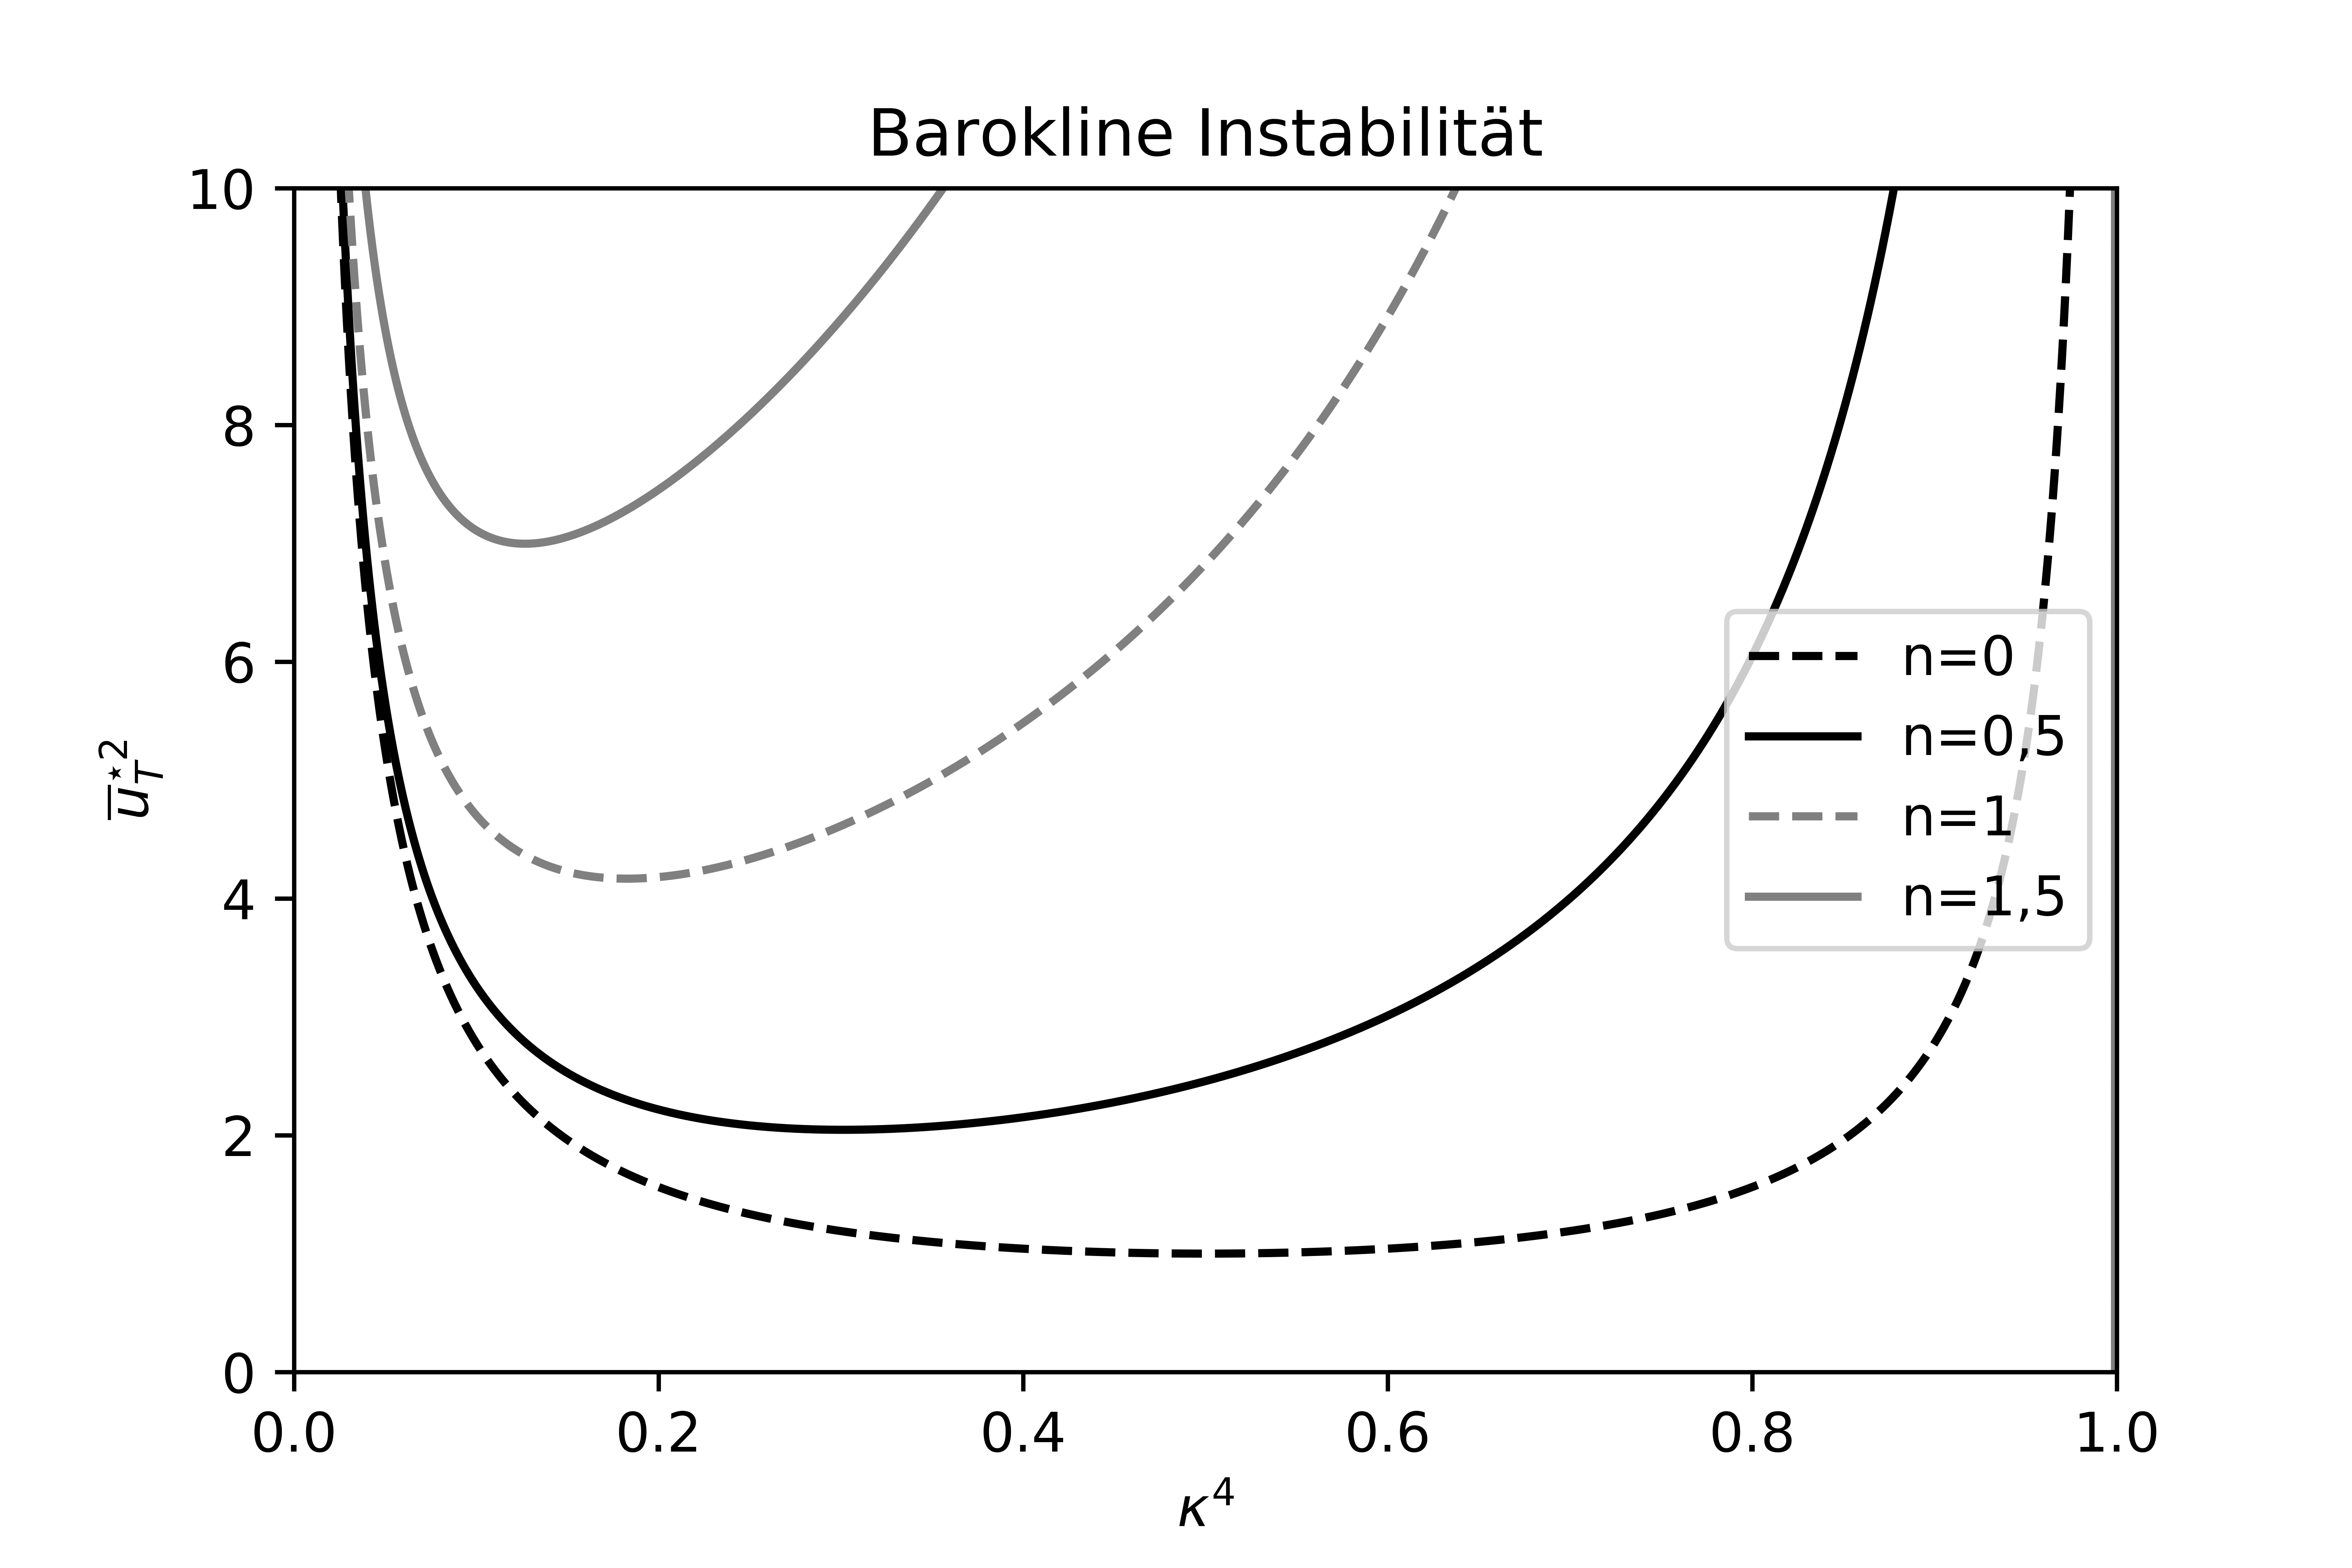
\includegraphics[width = .65\textwidth]{figs/baro_inst.png}
\caption{Die für gewisse Wachstumsraten notwendigen Windscherungen als Funktion der Wellenzahl.}
\label{fig:barokline_instabilitaet}
\end{figure}

Abb. \ref{fig:barokline_instabilitaet} zeigt die für unterschiedliche Wellenzahlen und Wachstumsraten notwendigen thermischen Windscherungen. Aus den Definitionen von $\kappa$ und $\newoverline{u}^\star_T$ wird klar, dass man sich bei abnehmender thermischer Stabilität in dieser Darstellung nach links oben bewegt, also in Richtung barokliner Labilität.

Bei der baroklinen Instabilität wird potentielle Energie der Schichtung, welche durch das Strahlungsfeld immer wieder neu erzeugt wird, in kinetische Energie des Horizontalwindes umgewandelt, bevor sie dissipiert wird.

\subsection{Kelvin-Helmholtz-Instabilität}
\label{sec:kelvin-helmholtz-instabilitaet}\index{Kelvin-Helmholtz-Instabilität}

Die \textit{Kelvin-Helmholtz-Instabilität} bezeichnet das Brechen von Schichtungswellen in einer vertikal gescherten Horizontalströmung.

\subsubsection{In diskreter Schichtung}
\label{sec:in_diskreter_schichtung}\index{Schichtung!diskrete!Kelvin-Helmholtz-Instabilität}\index{diskrete Schichtung!Kelvin-Helmholtz-Instabilität}\index{Kelvin-Helmholtz-Instabilität!in diskreter Schichtung}

Die Bewegung sei y-symmetrisch, betrachtet wird also die xz-Ebene. Die xy-Ebene falle mit der Gleichgewichtslage einer Phasengrenze zusammen. Das Medium oberhalb der Grenzschicht ($z > 0$) erhält den Index 1, das Medium darutner ($z < 0$) den Index 2. Die Medien seien barotrop und inkompressibel. Zum Zeitpunkt $t = 0$ werde das Strömungsfeld durch
%
\begin{align}
U_1 > 0, && U_2 > 0, && V_1 = V_2 = W_1 = W_2 = 0
\end{align}
%
beschrieben. Die Coriolis-Kraft wird vernachlässigt. Es gilt
%
\begin{align}
\nabla \times \mathbf{v}_1 = \nabla \times \mathbf{v}_2 = \mathbf{0}.
\end{align}
%
Aufgrund des Zirkulationssatzes in der Form Glg. \eqref{eq:circ_theorem_mod_1} gilt dies auch für $t > 0$, solange sich die Medien nicht durchmischen. Daher beschreibt man die Geschwindigkeitsfelder durch zwei Stromfunktionen
%
\begin{align}
\psi_1 = U_1x + \psi_1', && \psi_2 = U_2 x + \psi_2',\label{eq:khi_discrete_stream}
\end{align}
%
wobei die gestrichenen Größen für die Störungen stehen. Aufgrund der Divergenzfreiheit gilt
%
\begin{align}
\Delta\psi_1' = \Delta\psi_2' = 0\label{eq:khi_deriv_laplace}.
\end{align}
%
Die Auslenkung der Phasengrenze sei mit $\zeta$ bezeichnet. Mit $\mathbf{n}$ als Normalenvektor der Oberfläche und $\zeta$ als Oberflächenauslenkung gilt die kinematische Randbedingung
%
\begin{align}
\mathbf{n}\cdot\nabla\psi_1 = \mathbf{n}\cdot\left(\frac{\partial\zeta}{\partial t}\mathbf{e}_z\right) = \mathbf{n}\cdot\nabla\psi_2\text{ bei }z = \zeta.\label{eq:khi_discrete_kbc}
\end{align}
%
Mit Vernachlässigung der Oberflächenspannung folgt die dynamische Randbedingung\index{dynamische Randbedingung}\index{Randbedingung!dynamische}
%
\begin{align}
p_1 = p_2\text{ bei }z = \zeta.\label{eq:khi_discrete_dbc}
\end{align}
%
Für den Normalenvektor $\mathbf{n}$ gilt
%
\begin{align}
\mathbf{n} = \frac{1}{\sqrt{1 + \left(\frac{\partial\zeta}{\partial x}\right)^2}}\left(\begin{array}{c}
-\frac{\partial\zeta}{\partial x}\\
1\end{array}\right).
\end{align}
%
Die kinematische Randbedidngung Glg. \eqref{eq:khi_discrete_kbc} wird damit zu
%
\begin{align}
-\left(U_1 + \frac{\partial\psi_1'}{\partial x}\right)\frac{\partial\zeta}{\partial x} + \frac{\partial\psi_1'}{\partial z} = \frac{\partial\zeta}{\partial t} = -\left(U_2 + \frac{\partial\psi_2'}{\partial x}\right)\frac{\partial\zeta}{\partial x} + \frac{\partial\psi_2'}{\partial z}\text{ bei }z = \zeta,
\end{align}
%
wobei der Wurzelausdruck herausmultipliziert wurde. Um diesen Ausdruck zu linearisieren, wendet man ihn bei $z = 0$ an und vernachlässigt quadratische Terme:
%
\begin{align}
-U_1\frac{\partial\zeta}{\partial x} + \frac{\partial\psi_1'}{\partial z} = \frac{\partial\zeta}{\partial t} = -U_2\frac{\partial\zeta}{\partial x} + \frac{\partial\psi_2'}{\partial z}\text{ bei }z = 0\label{eq:khi_discrete_deriv_kbc}
\end{align}
%
Da das Strömungsfeld rotationsfrei ist und man außerdem von einem idealen Fluid ausgeht, kann man die zeitabhängigen Bernoulli-Gleichungen (s. Glg. \eqref{eq:bernoulli_t_dependant}) der beiden Schichten
%
\begin{align}
\frac{\partial\psi_1}{\partial t} + \frac{1}{2}\left|\nabla\psi_1\right|^2 + \frac{p_1}{\rho_1} + gz & = C,\\
\frac{\partial\psi_2}{\partial t} + \frac{1}{2}\left|\nabla\psi_2\right|^2 + \frac{p_2}{\rho_2} + gz & = C_2
\end{align}
%
mit reellen Konstanten $C, C_2$ aufstellen. Die dynamische Randbedingung Glg. \eqref{eq:khi_discrete_dbc} impliziert bei $z = \zeta$ die Identität
%
\begin{align}
\rho_1\left(C - \frac{\partial\psi_1}{\partial t} - \frac{1}{2}\left|\nabla\psi_1\right|^2 - gz\right) = \rho_2\left(C_2 - \frac{\partial\psi_2}{\partial t} - \frac{1}{2}\left|\nabla\psi_2\right|^2 - gz\right).\label{eq:khi_discrete_deriv_1}
\end{align}
%
Ohne Störung gilt
%
\begin{align}
\rho_1\left(C - \frac{1}{2}U_1^2\right) = \rho_2\left(C_2 - \frac{1}{2}U_2^2\right).\label{eq:khi_discrete_deriv_2}
\end{align}
%
Subtrahieren von Glg. \eqref{eq:khi_discrete_deriv_2} von Glg. \eqref{eq:khi_discrete_deriv_1} führt zu
%
\begin{align}
\rho_1\left(-\frac{\partial\psi_1}{\partial t} + \frac{1}{2}U_1^2 - \frac{1}{2}\left|\nabla\psi_1\right|^2 - gz\right) = \rho_2\left(-\frac{\partial\psi_2}{\partial t} + \frac{1}{2}U_2^2 - \frac{1}{2}\left|\nabla\psi_2\right|^2 - gz\right),\label{eq:khi_discrete_deriv_3}
\end{align}
%
was bei $z = \zeta$ gilt. Mit den Glg.en \eqref{eq:khi_discrete_stream} - \eqref{eq:khi_discrete_stream} folgt
%
\begin{align}
\frac{1}{2}\left|\nabla\psi_j\right|^2 & =  \frac{1}{2}\left(U_j^2 + \left(\frac{\partial\psi_j'}{\partial x}\right)^2 + 2U_j\frac{\partial\psi_j'}{\partial x} + \left(\frac{\partial\psi_j'}{\partial z}\right)^2\right)
\end{align}
%
für $j = 1, 2$. Setzt man dies in Glg. \eqref{eq:khi_discrete_deriv_3} ein, erhält man
%
\begin{align}
& \rho_1\left(-\frac{\partial\psi_1}{\partial t} - \frac{1}{2}\left(\frac{\partial\psi_1'}{\partial x}\right)^2 - U_1\frac{\partial\psi_1'}{\partial x} - \frac{1}{2}\left(\frac{\partial\psi_1'}{\partial z}\right)^2 - gz\right)\nonumber\\
& = \rho_2\left(-\frac{\partial\psi_2}{\partial t} - \frac{1}{2}\left(\frac{\partial\psi_1'}{\partial x}\right)^2 - U_2\frac{\partial\psi_1'}{\partial x} - \frac{1}{2}\left(\frac{\partial\psi_1'}{\partial z}\right)^2 - gz\right),\label{eq:khi_discrete_deriv_4}
\end{align}
%
bei $z = \zeta.$ Diese Gleichung linearisiert man, indem man sie bei $z = 0$ auswertet und die quadratischen Terme vernachlässigt:
%
\begin{align}
\rho_1\left(\frac{\partial\psi_1}{\partial t} + U_1\frac{\partial\psi_1'}{\partial x} + g\zeta\right) = \rho_2\left(\frac{\partial\psi_2}{\partial t} + U_2\frac{\partial\psi_1'}{\partial x} + g\zeta\right)\label{eq:khi_discrete_deriv_5}
\end{align}
%
Nun macht man für $j = 1, 2$ den Ansatz
%
\begin{align}
\psi_j' = A_j\left(z\right)\exp\left(ikx - i\omega t\right).
\end{align}
%
Mit den Laplace-Gleichungen Glg. \eqref{eq:khi_deriv_laplace} folgt
%
\begin{align}
-k^2A_j + \frac{d^2A_j}{dz^2} & = 0.
\end{align}
%
Die Lösungen sind von der Form
%
\begin{align}
A_j\left(z\right) = A_\pm\exp\left(\pm kz\right).
\end{align}
%
Mit den Festlegungen
%
\begin{align}
\lim_{z \to\infty} \psi_1' = 0, && \lim_{z \to -\infty} \psi_2' = 0,
\end{align}
%
welche bedeuten, dass die Störung in der Unendlichkeit verschwinden soll, folgen
%
\begin{align}
\psi_1' = A_-\exp\left[ikx - i\omega t - kz\right], && \psi_2' = A_+\exp\left[ikx - i\omega t + kz\right].
\end{align}
%
Für die Oberflächenauslenkung nimmt man entsprechend
%
\begin{align}
\zeta = \zeta_0\exp\left(ikx - i\omega t\right)
\end{align}
%
an. Setzt man dies in die Glg.en \eqref{eq:khi_discrete_deriv_kbc} und \eqref{eq:khi_discrete_deriv_5} ein, erhält man
%
\begin{align}
-U_1ik\zeta_0 - kA_- & = -i\omega\zeta_0 = -U_2ik\zeta_0 + kA_+,\label{eq:khi_discrete_deriv_6}\\
\rho_1\left(-i\omega A_- + ikU_1A_- + g\zeta_0\right) & = \rho_2\left(-i\omega A_+ + ikU_2A_+ + g\zeta_0\right).\label{eq:khi_discrete_deriv_7}
\end{align}
%
Glg. \eqref{eq:khi_discrete_deriv_6} impliziert
%
\begin{align}
A_- = \frac{i}{k}\zeta_0\left(\omega - U_1k\right), && A_+ = \frac{i}{k}\zeta_0\left(U_2k - \omega\right).
\end{align}
%
Setzt man dies in Glg. \eqref{eq:khi_discrete_deriv_7} ein, folgt
%
\begin{align}
\rho_1\left(-i\omega\frac{i}{k}\zeta_0\left(\omega - U_1k\right) + ikU_1\frac{i}{k}\zeta_0\left(\omega - U_1k\right) + g\zeta_0\right) & = \rho_2\left(-i\omega\frac{i}{k}\zeta_0\left(U_2k - \omega\right) + ikU_2\frac{i}{k}\zeta_0\left(U_2k - \omega\right) + g\zeta_0\right)\nonumber\\
\Leftrightarrow\rho_1\left(\frac{\omega}{k}\left(\omega - U_1k\right) - U_1\left(\omega - U_1k\right) + g\right) & = \rho_2\left(\frac{\omega}{k}\left(U_2k - \omega\right) - U_2\left(U_2k - \omega\right) + g\right)\nonumber\\
\Leftrightarrow\rho_1\left(\omega\left(\omega - U_1k\right) - kU_1\left(\omega - U_1k\right) + kg\right) & = \rho_2\left(\omega\left(U_2k - \omega\right) - U_2k\left(U_2k - \omega\right) + kg\right).
\end{align}
%
Dies ist eine quadratische Gleichung für $\omega$, also eine Dispersionsrelation. Weitere algebraische Umformung ergibt
%
\begin{align}
\omega^2 - 2k\omega\frac{\rho_1U_1 + \rho_2U_2}{\rho_1 + \rho_2} - kg\frac{\rho_2 - \rho_1}{\rho_1 + \rho_2} + k^2\frac{U_1^2\rho_1 + U_2^2\rho_2}{\rho_1 + \rho_2} = 0
\end{align}
%
Dies ergibt zwei Lösungen für die Kreisfrequenz:
%
\begin{align}
\omega_\pm & = \frac{\rho_1U_1k + \rho_2U_2k}{\rho_1 + \rho_2} \pm \left[kg\frac{\rho_2 - \rho_1}{\rho_1 + \rho_2} - k^2\frac{U_1^2\rho_1\rho_2 + U_2^2\rho_1\rho_2 - 2\rho_1\rho_2U_1U_2}{\left(\rho_1 + \rho_2\right)^2}\right]^{1/2}\nonumber\\
\Leftrightarrow\omega_\pm & = \frac{\rho_1U_1k + \rho_2U_2k}{\rho_1 + \rho_2} \pm \left[kg\frac{\rho_2 - \rho_1}{\rho_1 + \rho_2} - k^2\rho_1\rho_2\frac{\left(U_1 - U_2\right)^2}{\left(\rho_1 + \rho_2\right)^2}\right]^{1/2}
\end{align}
%
Instabilität liegt vor im Fall
%
\begin{align}
kg\frac{\rho_2 - \rho_1}{\rho_1 + \rho_2} &- k^2\rho_1\rho_2\frac{\left(U_1 - U_2\right)^2}{\left(\rho_1 + \rho_2\right)^2} < 0\nonumber\\
\Leftrightarrow kg\frac{\rho_2 - \rho_1}{\rho_1 + \rho_2} & < k^2\rho_1\rho_2\frac{\left(U_1 - U_2\right)^2}{\left(\rho_1 + \rho_2\right)^2}\nonumber
\end{align}
\begin{center}
\doublebox{\parbox{\textwidth}{
\begin{center}
\begin{align}
\Leftrightarrow g\left(\rho_2^2 - \rho_1^2\right) & < k\rho_1\rho_2\left(U_1 - U_2\right)^2,\label{eq:khi_discrete_cond}
\end{align}
\end{center}
}}
\end{center}
%
also wenn
%
\begin{itemize}
\item die Dichtedifferenz klein genug ist,
\item die Welle kurz genug ist oder die
\item Geschwindigkeitsdifferenz groß genug ist.
\end{itemize}
%
Ein Beispiel ist das Entstehen von Wasseroberflächenwellen unter Windeinwirkung. Man kann davon ausgehen, dass fast immer spektrale Komponenten im Windfeld vorhanden sind, die die Bedingung Glg. \eqref{eq:khi_discrete_cond} erfüllen. Die weitere zeitliche Entwicklung des Systems kann unterschiedlich aussehen, z. B. ist diese abhängig davon, ob sich die Medien durchmischen können oder nicht.

\subsubsection{Schichtung}
\label{sec:schichtung}\index{kontinuierliche Schichtung!Kelvin-Helmholtz-Instabilität}\index{Kelvin-Helmholtz-Instabilität!in kontinuierlicher Schichtung}

Man betrachtet wieder die xz-Ebene und vernachlässigt die Coriolis-Beschleunigung. Außerdem macht man die Boussinesq-Approximation (s. Absch. \ref{sec:boussinesq-approximation}). Impuls-, Kontinuitätsgleichung und Erster Hauptsatz der Thermodynamik lauten mit $\sigma$ als potentieller Dichte
%
\begin{align}
\frac{\partial u}{\partial t} + u\frac{\partial u}{\partial x} + w\frac{\partial w}{\partial z} & = -\frac{1}{\rho}\frac{\partial p}{\partial x},\\
\frac{\partial w}{\partial t} + u\frac{\partial w}{\partial x} + w\frac{\partial w}{\partial z} & = -\frac{1}{\rho}\frac{\partial p}{\partial z} - g,\\
\frac{\partial u}{\partial x} + \frac{\partial w}{\partial z} & = 0,\\
\frac{\partial\sigma}{\partial t} + u\frac{\partial\sigma}{\partial x} + w\frac{\partial\sigma}{\partial z} & = 0.
\end{align}
%
Nun geht man von einem vertial gescherten Hintergrundwindfeld $\newoverline{u}\left(z\right) = u\left(x, z, t\right) - u'\left(x, z, t\right)$ aus, der vertikale Hintergrundwind $\newoverline{w}$ verschwinde. Die Hintergrunddichte $\newoverline{\rho}\left(z\right) = \rho\left(x, z, t\right) - \rho'\left(x, z, t\right)$ sei in hydrostatischer Balance mit dem Hintergrunddruckfeld $\newoverline{p}\left(z\right) = p\left(x, z, t\right) - p'\left(x, z, t\right)$, also
%
\begin{align}
\frac{\partial\newoverline{p}}{\partial z} & = -g\newoverline{\rho}.\label{eq:khi_deriv_1}
\end{align}
%
Setzt man dies in die Gleichungen ein und linearisiert sie, erhält man
%
\begin{align}
\frac{\partial u'}{\partial t} + \newoverline{u}\frac{\partial u'}{\partial x} + w\frac{\partial\newoverline{u}}{\partial z} & = -\frac{1}{\rho}\frac{\partial p'}{\partial x} \approx -\frac{1}{\newtilde{\rho}}\frac{\partial p'}{\partial x},\\
\frac{\partial w}{\partial t} + \newoverline{u}\frac{\partial w}{\partial x} & = -\frac{1}{\rho}\frac{\partial p}{\partial z} - g \approx -\frac{1}{\newtilde{\rho}}\frac{\partial p}{\partial z} - \frac{g\rho}{\newtilde{\rho}} = -\frac{1}{\newtilde{\rho}}\frac{\partial p'}{\partial z} - \frac{g\rho'}{\newtilde{\rho}},\\
\frac{\partial u'}{\partial x} + \frac{\partial w}{\partial z} & = 0,\\
\frac{\partial\sigma'}{\partial t} + \newoverline{u}\frac{\partial\sigma'}{\partial x} + w\frac{\partial\newoverline{\sigma}}{\partial z} & = 0.
\end{align}
%
In der x-Komponente der Impulsgleichung wurde im Nenner des Druckgradientterms $\rho \to \newtilde{\rho}$ ersetzt, wobei $\newtilde{\rho}$ eine als homogen angenommene mittlere Dichte bezeichnet; in der z-Komponente wurde die rechte Seite mit $\frac{\rho}{\newtilde{\rho}}$ multipliziert, bevor Glg. \eqref{eq:khi_deriv_1} eingesetzt wurde. Die Störung der Strömung ist divergenzfrei, daher setzt man eine Stromfunktion $\psi = \psi\left(x, z, t\right)$ mit
%
\begin{align}
u' & = \frac{\partial\psi}{\partial z},\\
w & = -\frac{\partial\psi}{\partial x}.
\end{align}
%
an. Damit ist die Kontinuitätsgleichung automatisch erfüllt. Die verbleibenden drei Gleichungen lauten
%
\begin{align}
\frac{\partial^2\psi}{\partial t\partial z} + \newoverline{u}\frac{\partial^2\psi}{\partial z\partial x} - \frac{\partial\psi}{\partial x}\frac{\partial\newoverline{u}}{\partial z} & = -\frac{1}{\newtilde{\rho}}\frac{\partial p'}{\partial x},\\
-\frac{\partial^2\psi}{\partial t\partial x} - \newoverline{u}\frac{\partial^2\psi}{\partial x^2} & = -\frac{1}{\newtilde{\rho}}\frac{\partial p'}{\partial z} - \frac{g\rho'}{\newtilde{\rho}},\\
\frac{\partial\sigma'}{\partial t} + \newoverline{u}\frac{\partial\sigma'}{\partial x} - \frac{\partial\psi}{\partial x}\frac{\partial\newoverline{\sigma}}{\partial z} & = 0.
\end{align}
%
Nun macht man weiterhin die Ansätze
%
\begin{align}
\psi\left(x, z, t\right) = \psi_0\left(z\right)\exp\left[ik\left(x - ct\right)\right], && p'\left(x, z, t\right) = p_0\left(z\right)\exp\left[ik\left(x - ct\right)\right],\\
\rho'\left(x, z, t\right) = \rho_0\left(z\right)\exp\left[ik\left(x - ct\right)\right], && \sigma'\left(x, z, t\right) = \sigma_0\left(z\right)\exp\left[ik\left(x - ct\right)\right].
\end{align}
%
Daraus folgt
%
\begin{align}
-ikc\frac{d\psi_0}{dz} + \newoverline{u}ik\frac{d\psi_0}{dz} - ik\psi_0\frac{\partial\newoverline{u}}{\partial z} & = -ik\frac{p_0}{\newtilde{\rho}},\\
-k^2c\psi_0 + \newoverline{u}k^2\psi_0 & = -\frac{1}{\newtilde{\rho}}\frac{dp_0}{dz} -g\frac{\rho_0}{\newtilde{\rho}},\\
-ikc\sigma_0 + \newoverline{u}ik\sigma_0 -ik\psi_0\frac{d\newoverline{\sigma}}{dz} & = 0.
\end{align}
%
Dies ergibt vereinfacht
%
\begin{align}
-c\frac{d\psi_0}{dz} + \newoverline{u}\frac{d\psi_0}{dz} - \psi_0\frac{\partial\newoverline{u}}{\partial z} & = -\frac{p_0}{\newtilde{\rho}},\\
\psi_0k^2\left(\newoverline{u} - c\right) & = -\frac{1}{\newtilde{\rho}}\frac{dp_0}{dz} - g\frac{\rho_0}{\newtilde{\rho}}, \label{eq:khi_deriv_2}\\
\sigma_0\left(\newoverline{u} - c\right) - \psi_0\frac{d\newoverline{\sigma}}{dz} & = 0.\label{eq:khi_deriv_3}
\end{align}
%
Differenziert man die erste Gleichung nach $z$, erhält man
%
\begin{align}
\frac{d^2\psi_0}{dz^2}\left(\newoverline{u} - c\right) - \psi_0\frac{d^2\newoverline{u}}{dz^2} & = -\frac{1}{\newtilde{\rho}}\frac{dp_0}{dz}.
\end{align}
%
Setzt man hier Glg. \eqref{eq:khi_deriv_2} ein, folgt
%
\begin{align}
\left(\newoverline{u} - c\right)\left[\frac{d^2\psi_0}{dz^2} - k^2\psi_0\right] - \psi_0\frac{d^2\newoverline{u}}{dz^2} - g\frac{\rho_0}{\newtilde{\rho}} & = 0.
\end{align}
%
Um $\rho_0$ zu eliminieren, stellt man zunächst Glg. \eqref{eq:khi_deriv_3} nach $\sigma_0$ um und erhält
%
\begin{align}
\sigma_0 & = \frac{\psi_0}{\newoverline{u} - c}\frac{d\newoverline{\sigma}}{dz}.
\end{align}
%
O. B. d. A. kann man das Referenzniveau in das gerade betrachtete Niveau legen und $\rho_0 = \sigma_0$ verwenden. Dies ergibt eingesetzt
%
\begin{align}
\left(\newoverline{u} - c\right)\left[\frac{d^2\psi_0}{dz^2} - k^2\psi_0\right] -\psi_0\frac{d^2\newoverline{u}}{dz^2} - \frac{\psi_0}{\newoverline{u} - c}\frac{g}{\newtilde{\rho}}\frac{d\newoverline{\sigma}}{dz} & = 0.
\end{align}
%
Hier setzt man die Brunt-Väisälä-Frequenz\index{Brunt-Väisälä-Frequenz}
%
\begin{align}
N^2 \coloneqq -\frac{g}{\newtilde{\rho}}\frac{d\newoverline{\sigma}}{dz}
\end{align}
%
ein und erhält
%
\begin{align}
\left(\newoverline{u} - c\right)\left(\frac{d^2}{dz^2} - k^2\right)\psi + \left(\frac{N^2}{\newoverline{u} - c} - \frac{d^2\newoverline{u}}{dz^2}\right)\psi = 0.\label{eq:taylor-goldstein}
\end{align}
%
Diese Gleichung bezeichnet man als \textit{Taylor-Goldstein-Gleichung}\index{Taylor-Goldstein-Gleichung}. Es handelt sich um ein Eigenwertproblem $\left\{\psi, c\right\}$ an die Funktion $\psi$ mit dem Eigenwert $c$ abhängig von $\newoverline{u}\left(z\right)$. Ist $\left\{\psi, c\right\}$ eine Lösung, so ist $\left\{\psi^\star, c^\star\right\}$ ebenfalls eine Lösung. Ein postiver Imaginärteil von $c$ bedeutet, dass $\psi$ eine instabile Lösung ist. Eine Scherung $\newoverline{u} = \newoverline{u}\left(z\right)$ ist genau dann stabil, wenn alle Lösungen von Glg. \eqref{eq:taylor-goldstein} reelle Eigenwerte haben. Man geht nun weiter davon aus, dass bei $z = 0, H$ die Randbedingungen $w = 0$ gelten, daraus folgt
%
\begin{align}
\psi\left(0\right) = \psi\left(H\right) = 0.
\end{align}
%
Nun definiert man $\phi$ durch
%
\begin{align}
\psi = \sqrt{\newoverline{u} - c}\phi.
\end{align}
%
Differenzieren nach $z$ ergibt
%
\begin{align}
\frac{d\psi}{dz} & = \frac{1}{2}\frac{1}{\sqrt{\newoverline{u} - c}}\phi\frac{d\newoverline{u}}{dz} + \sqrt{\newoverline{u} - c}\frac{d\phi}{dz},\\
\Rightarrow\frac{d^2\psi}{dz^2} & = \frac{1}{\sqrt{\newoverline{u} - c}}\frac{d\newoverline{u}}{dz}\frac{d\phi}{dz} - \frac{1}{4}\frac{1}{\sqrt{\newoverline{u} - c}^3}\phi\left(\frac{d\newoverline{u}}{dz}\right)^2 + \frac{1}{2}\frac{1}{\sqrt{\newoverline{u} - c}}\frac{d^2\newoverline{u}}{dz^2}\phi + \sqrt{\newoverline{u} - c}\frac{d^2\phi}{dz^2}.
\end{align}
%
Setzt man dies in Glg. \eqref{eq:taylor-goldstein} ein und dividiert durch $\sqrt{\newoverline{u} - c}$, erhält man 
%
\begin{align}
\frac{d}{dz}\left[\left(\newoverline{u} - c\right)\frac{d\phi}{dz}\right] - \left[k^2\left(\newoverline{u} - c\right) + \frac{1}{2}\frac{d^2\newoverline{u}}{dz^2} + \frac{1}{\newoverline{u} - c}\left(\frac{1}{4}\left(\frac{d\newoverline{u}}{dz}\right)^2 - N^2\right)\right]\phi = 0.\label{eq:khi_deriv_4}
\end{align}
%
Die Randbedingungen bleiben unter der Annahme $c \not= \newoverline{u}$
%
\begin{align}
\phi\left(0\right) = \phi\left(H\right) = 0.
\end{align}
%
Die Glg. \eqref{eq:khi_deriv_4} wird nun mit $\phi^\star$ multipliziert:
%
\begin{align}
\phi^\star\frac{d}{dz}\left[\left(\newoverline{u} - c\right)\frac{d\phi}{dz}\right] - \left[k^2\left(\newoverline{u} - c\right) + \frac{1}{2}\frac{d^2\newoverline{u}}{dz^2} + \frac{1}{\newoverline{u} - c}\left(\frac{1}{4}\left(\frac{d\newoverline{u}}{dz}\right)^2 - N^2\right)\right]\left|\phi\right|^2 = 0.\label{eq:khi_deriv_5}
\end{align}
%
Inegriert man den ersten Term von $0$ bis $H$, folgt mittels partieller Integration
%
\begin{align}
\int_0^H\phi^\star\frac{d}{dz}\left[\left(\newoverline{u} - c\right)\frac{d\phi}{dz}\right]dz & = -\int_0^H\left(\newoverline{u} - c\right)\left|\frac{d\phi}{dz}\right|^2dz.
\end{align}
%
Glg. \eqref{eq:khi_deriv_5} wird nun von $0$ nach $H$ integriert:
%
\begin{align}
\int_0^H\left[N^2 - \frac{1}{4}\left(\frac{d\newoverline{u}}{dz}\right)^2\right]\frac{\left|\phi\right|^2}{\newoverline{u} - c}dz & = \int_0^H\left(\newoverline{u} - c\right)\left(\left|\frac{d\phi}{dz}\right|^2 + k^2\left|\phi\right|^2\right) + \frac{1}{2}\frac{d^2\newoverline{u}}{dz^2}\left|\phi\right|^2dz.\label{eq:khi_deriv_6}
\end{align}
%
Man schreibt nun für die Phasengeschwindigkeit
%
\begin{align}
c = c_r + ic_i
\end{align}
%
mit $c_r, c_i\in\mathbb{R}$. Der Imaginärteil von Glg. \eqref{eq:khi_deriv_6} schreibt sich als
%
\begin{align}
c_i\int_0^H\left[N^2 - \frac{1}{4}\left(\frac{d\newoverline{u}}{dz^2}\right)^2\right]\frac{\left|\phi\right|^2}{\left|\newoverline{u} - c\right|^2}dz & = -c_i\int_0^H\left(\left|\frac{d\phi}{dz}\right|^2 + k^2\left|\phi\right|^2\right)dz\nonumber\\
\Rightarrow c_i\int_0^H\left[N^2 - \frac{1}{4}\left(\frac{d\newoverline{u}}{dz^2}\right)^2\right]\frac{\left|\phi\right|^2}{\left|\newoverline{u} - c\right|^2} + \left|\frac{d\phi}{dz}\right|^2 + k^2\left|\phi\right|^2dz & = 0.
\end{align}
%
Gilt $N^2 - \frac{1}{4}\left(\frac{d\newoverline{u}}{dz^2}\right)^2 > 0$ überall im Intervall $\left(0, H\right), $ so ist $c_i = 0$. Man definiert die \textit{Richardson-Zahl}\index{Richardson-Zahl} $R_i$ durch
%
\begin{center}
\doublebox{\parbox{\textwidth}{
\begin{center}
\begin{align}
R_i \coloneqq \frac{N^2}{\left(\frac{d\newoverline{u}}{dz}\right)^2}.
\end{align}
\end{center}
}}
\end{center}
%
Die Frequenz
%
\begin{center}
\doublebox{\parbox{\textwidth}{
\begin{center}
\begin{align}
M \coloneqq \frac{d\newoverline{u}}{dz}
\end{align}
\end{center}
}}
\end{center}
%
bezeichnet man als \index{Prandtl-Frequenz}\textit{Prandtl-Frequenz}. Die Bedingung
%
\begin{center}
\doublebox{\parbox{\textwidth}{
\begin{center}
\begin{align}
R_i > \frac{1}{4}\text{ überall in }\left(0, H\right)
\end{align}
\end{center}
}}
\end{center}
%
ist hinreichend für Stabiilität.

\subsection{Thermische Instabilität}
\label{sec:thermische_instabilitaet}\index{thermische Instabilität}\index{Instabilität!thermische}

Die Atmosphäre habe an einem gegebenen Punkt die Schichtung $T = T\left(z\right)$. Üblicherweise ist
%
\begin{align}
\frac{\partial T}{\partial z}<0, 
\end{align}
%
bei $\frac{\partial T}{\partial z}>0$ spricht man von einer \index{Inversion}\textit{Inversion}. Der trockenadiabatische Temperaturgradient ist nach Glg. \eqref{eq:trockenad_tempgradient} durch
%
\begin{align}
\Gamma_d = \frac{g}{c^{(p)}}
\end{align}
%
definiert. Im Fall
%
\begin{align}
\frac{\partial T}{\partial z}< - \Gamma_d
\end{align}
%
ist die Schichtung \textit{lokal instabil}, solange die Luft dabei ungesättigt bleibt.

Ist die Luft jedoch gesättigt, findet bei der Abkühlung, die infolge der Hebung stattfindet, Kondensation oder Resublimation statt, wobei Phasenübergangswärme frei wird. Lenkt man das Teilchen bei $z$ vertikal aus, ergibt sich das \textit{lifted condensation level (LCL)}\index{lifted condensation level (LCL)}\index{Hebungskondensationsniveau (HKN)}\index{HKN}\index{LCL} $z_L$ als die Höhe $z_{\text{LCL}}$, in der es gesättigt wäre, also erfüllt es die Gleichung
%
\begin{align}
p_v^{(S)}\left(T\left(z\right) - \Gamma_d\left(z_{\text{LCL}} - z\right)\right) \equiv p_v\left(z\right)\left(1 - \frac{\Gamma_d\left(z_{\text{LCL}} - z\right)}{T\left(z\right)}\right)^{\frac{g}{R_d\Gamma_d}}
\end{align}
%
Man geht bei der anschließenden weiteren Hebung zunächst davon aus, dass das komplette Wasser in der Wolke verbleibt, was man als \textit{reversible Feuchtadiabate}\index{reversible Feuchtadiabate}\index{Feuchtadiabate!reversible} bezeichnet; gelegentlich wird statt feuchtadiabatisch auch das Wort pseudoadiabatisch\index{pseudoadiabatisch} verwendet, da die Frage, ob dieser Prozess adiabatisch ist oder nicht davon abhängt, welches System man betrachtet: betrachtet man die Luft inklusive der Kondensate als System, ist der Prozess adiabatisch\index{adiabatisch}, da es keine Wärme mit seiner Umgebung austauscht; betrachtet man hingegen nur die Gasphase, so ist der Prozess diabatisch\index{diabatisch}, da latente Wärme\index{latente Wärme}\index{Wärme!latente} austauscht. Bei der \textit{irreversiblen Feuchtadiabate}\index{irreversible Feuchtadiabate}\index{Feuchtadiabate!irreversible}, worauf in Absch. \ref{sec:cape} näher eingegangen wird, wird hingegen davon ausgegangen, dass das gesamte Wasser ausregnet. Dies soll nun betrachtet werden. Nehme also an, dass die Luft in einem Teilchen mit dem Volumen $V$ und der konstanten Masse $m$ aus einem Gemisch aus feuchter Luft und Kondensationsprodukten einer Phase besteht, wobei alle Komponenten die gleiche Temperatur $T$ haben sollen. Mit dem Ersten Hauptsatz der Thermodynamik Glg. \eqref{eq:td1_ideal_gas} erhält man
%
\begin{align}
& c^{(v)}\frac{dT}{dz} + p\frac{d}{dz}\frac{1}{\rho} = \frac{1}{\rho}\frac{dq}{dz}\nonumber\\
\Rightarrow\frac{dT}{dz} & = \frac{1}{c^{(v)}}\left[\frac{1}{\rho}\frac{dq}{dz} - p\frac{d}{dz}\frac{1}{\rho}\right] = \frac{1}{\rho c^{(v)}}\left[\frac{dq}{dz} + \frac{p}{\rho}\frac{d\rho}{dz}\right] = -\frac{g}{c^{(v)}}\left[\frac{dq}{dp} + \frac{p}{\rho}\frac{d\rho}{dp}\right].\label{eq:feuchtad_deriv_1}
\end{align}
%
Hierbei wurde die hydrostatische Grundgleichung eingesetzt. Für die Wärmeleistung pro Volumen infolge des Phasenübergangs $dq$ gilt
%
\begin{align}
dq = \frac{c_{c}}{v}_hdm_c
\end{align}
%
mit $m_c$ als kondensiertet oder resublimierter Masse und $c_{c}$ als Phasenübergangswärme. Mit der Zustandsgleichung für Wasserdampf gilt
%
\begin{align}
p_v & = \rho_vR_vT\Rightarrow m_v = \frac{V_vp_v}{R_vT} = \frac{V_hp_v}{R_vT} = \frac{m_hR_hp_v^{(S)}\left(T\right)}{pR_v}\nonumber\\
\Rightarrow dm_c & = -dm_v = \frac{m_hR_hp_v^{(S)}\left(T\right)}{pR_v}\left(\frac{dp}{p} - \frac{dp_v^{(S)}}{p_v^{(S)}} + \frac{dm_c}{m_h}\right)\nonumber\\
\Rightarrow dm_c\left(1 - \frac{R_hp_v^{(S)}\left(T\right)}{pR_v}\right) & = \frac{m_hR_hp_v^{(S)}\left(T\right)}{pR_v}\left(\frac{dp}{p} - \frac{dp_v^{(S)}}{p_v^{(S)}}\right)\nonumber\\
\Rightarrow dm_c & = m_h\frac{\frac{dp}{p} - \frac{dp_v^{(S)}}{p_v^{(S)}}}{\frac{pR_v}{R_hp_v^{(S)}} - 1}.
\end{align}
%
Hierbei ist $p_v^{(S)} = p_v^{(S)}\left(T\right)$ der Sättigungsdampfdruck. Daraus folgt
%
\begin{align}
dq & = \frac{c_c}{T}\frac{dp - \frac{p}{p_v^{(S)}}dp_v^{(S)}}{\frac{pR_v}{p_v^{(S)}} - R_h}\nonumber\\
\Rightarrow\frac{dq}{dp} & = \frac{c_c}{\frac{pR_vT}{p_v^{(S)}} - R_hT}\left(1 - \frac{p}{p_v^{(S)}}\frac{dp_v^{(S)}}{dp}\right) = \frac{c_c}{\frac{pR_vT}{p_v^{(S)}} - TR_h}\left(1 + \frac{1}{g\rho}\frac{dT}{dz}\frac{p}{p_v^{(S)}}\frac{dp_v^{(S)}}{dT}\right)\nonumber\\
& = \frac{c_c}{TpR_v - Tp_v^{(S)}R_h}\left(p_v^{(S)} + \frac{p}{g\rho}\frac{dT}{dz}\frac{dp_v^{(S)}}{dT}\right)\nonumber\\
& = \frac{c_cp_v^{(S)}}{TpR_v - Tp_v^{(S)}R_h} + \frac{p}{Tg\rho}\frac{c_c}{pR_v - p_v^{(S)}R_h}\frac{dp_v^{(S)}}{dT}\frac{dT}{dz}.
\end{align}
%
Setzt man dies in Glg. \eqref{eq:feuchtad_deriv_1} ein und wendet ein weiteres Mal die Kettenregel an, erhält man
%
\begin{align}
\frac{dT}{dz} & = -\frac{g}{c^{(v)}}\Bigg[\frac{c_cp_v^{(S)}}{TpR_v - Tp_v^{(S)}R_h}\nonumber\\
& + \frac{p}{Tg\rho}\frac{c_c}{pR_v - p_v^{(S)}R_h}\frac{dp_v^{(S)}}{dT}\frac{dT}{dz} + \frac{p}{\rho}\frac{\partial\rho}{\partial p} - \frac{p}{g\rho^2}\frac{\partial\rho}{\partial T}\frac{dT}{dz}\Bigg].
\end{align}
%
Nun braucht man eine Zustandsgleichung. Für die Dichte gilt
%
\begin{align}
\rho = \rho_h + \rho_c = \frac{p}{R_hT} + \rho_c.
\end{align}
%
Man erhält damit
%
\begin{align}
\frac{dT}{dz} & = \frac{g}{c^{(v)}}\Bigg[ - \frac{c_cp_v^{(S)}}{TpR_v - Tp_v^{(S)}R_h}\nonumber\\
& - \frac{p}{Tg\rho}\frac{c_c}{pR_v - p_v^{(S)}R_h}\frac{dp_v^{(S)}}{dT}\frac{dT}{dz} - \frac{p}{\rho R_hT} - \frac{p^2}{R_hg\rho^2T^2}\frac{dT}{dz}\Bigg]\nonumber\\
& = \frac{g}{c^{(v)}}\Bigg[ - \frac{c_cp_v^{(S)}}{TpR_v - Tp_v^{(S)}R_h} - \frac{p}{Tg\rho}\frac{c_c}{pR_v - p_v^{(S)}R_h}\frac{dp_v^{(S)}}{dT}\frac{dT}{dz}\nonumber\\
& - 1 + \frac{\rho
_c}{\rho} - \frac{1}{g}\left(1 - \frac{\rho_c}{\rho}\right)\frac{p}{\rho T}\frac{dT}{dz}\Bigg].
\end{align}
%
Dies stellt man nun nach $\frac{dT}{dz}$ um:
%
\begin{align}
& \frac{dT}{dz}\left(1 + \frac{p}{Tc^{(v)}\rho}\frac{c_c}{pR_v - p_v^{(S)}R_h}\frac{dp_v^{(S)}}{dT} + \frac{1}{c^{(v)}}\left(1 - \frac{\rho_c}{\rho}\right)\frac{p}{\rho T}\right)\nonumber\\
& = \frac{g}{c^{(v)}}\left(\frac{\rho_c}{\rho} - 1\right) - \frac{gc_cp_v^{(S)}\left(T\right)}{c^{(v)}T\left(R_vp - p_v^{(S)}R_h\right)}\nonumber\\
\Rightarrow\frac{dT}{dz} & = -\frac{g}{c^{(p)}}\frac{1 - \frac{\rho_c}{\rho} + \frac{c_cp_v^{(S)}}{T\left(R_vp - p_v^{(S)}R_h\right)}}{\frac{c^{(v)}}{c^{(p)}} + \frac{p}{T\rho c^{(p)}}\frac{c_c}{pR_v - p_v^{(S)}R_h}\frac{dp_v^{(S)}}{dT} + \left(1 - \frac{\rho_c}{\rho}\right)\frac{p}{c^{(p)}T\rho}}\nonumber\\
& = -\Gamma_d\beta
\end{align}
%
Hierbei ist
%
\begin{center}
\doublebox{\parbox{\textwidth}{
\begin{center}
\begin{align}
\beta = \beta\left(p, T, \rho_c\right) \coloneqq\frac{1 - \frac{\rho_c}{\rho} + \frac{c_cp_v^{(S)}}{T\left(R_vp - p_v^{(S)}R_h\right)}}{\frac{c^{(v)}}{c^{(p)}} + \frac{p}{T\rho c^{(p)}}\frac{c_c}{pR_v - p_v^{(S)}R_h}\frac{dp_v^{(S)}}{dT} + \left(1 - \frac{\rho_c}{\rho}\right)\frac{p}{c^{(p)}T\rho}}.\label{eq:beta_malr}
\end{align}
\end{center}
}}
\end{center}
%
Für die Ableitung $\frac{dp_v^{(S)}}{dT}$ kann die Clausius-Clapeyron-Gleichung eingesetzt werden. Der sogenannte \textit{feuchtadiabatische Temperaturgradient}\index{feuchtadiabatischer Temperaturgradient}\index{Temperaturgradient!feuchtadiabatischer} wird nun durch
%
\begin{align}
\Gamma_h\coloneqq\Gamma_d\beta
\end{align}
%
definiert. Setzt man in Glg. \eqref{eq:beta_malr} $\rho_c = 0$ und $p_v \ll p$ ein, behält aber Terme mit $\frac{dp_v^{(S)}}{dT}$, folgt
%
\begin{align}
\frac{dT}{dz} & = -\frac{g}{c^{(p)}}\frac{1 + \frac{c_cp_v^{(S)}}{TR_vp}}{\frac{c^{(v)}}{c^{(p)}} + \frac{p}{T\rho c^{(p)}}\frac{c_c}{pR_v}\frac{dp_v^{(S)}}{dT} + \frac{p}{c^{(p)}T\rho}}.
\end{align}
%
Setzt man hier die Zustandsgleichung idealer Gase $p = \rho R_dT$ ein, erhält man den in der Literatur häufig angetroffene Ausdruck
%
\begin{align}
\frac{dT}{dz} & = -\frac{g}{c^{(p)}}\frac{1 + \frac{c_cp_v^{(S)}}{TR_vp}}{\frac{c^{(v)}}{c^{(p)}} + \frac{R_d}{c^{(p)}}\frac{c_c}{pR_v}\frac{dp_v^{(S)}}{dT} + \frac{c^{(p)} - c^{(v)}}{c^{(p)}}}\nonumber\\
\Leftrightarrow\frac{dT}{dz} & = -\frac{g}{c^{(p)}}\frac{1 + \frac{c_cp_v^{(S)}}{TR_vp}}{1 + \frac{R_dc_c}{R_vc^{(p)}p}\frac{dp_v^{(S)}}{dT}} \equiv -\Gamma_d\beta'
\end{align}
%
mit einem vereinfachten Faktor
%
\begin{align}
\beta'& = \beta'\left(p, T\right) \coloneqq\frac{1 + \frac{c_cp_v^{(S)}}{TR_vp}}{1 + \frac{\epsilon'c_c}{pc^{(p)}}\frac{dp_v^{(S)}}{dT}}\stackrel{\text{Glg. \eqref{eq:clausius-clapeyron_vereinfacht}}}{\approx}\frac{1 + \frac{c_cp_v^{(S)}}{TR_vp}}{1 + \frac{\epsilon'c_c^2p_v^{(S)}}{R_vc^{(p)}T^2p}}\nonumber
\end{align}
\begin{center}
\doublebox{\parbox{\textwidth}{
\begin{center}
\begin{align}
\Leftrightarrow\beta'&\stackrel{\text{Glg. \eqref{eq:mischungsverhaeltnis_vereinfacht}}}{\approx}\frac{1 + \frac{c_cr^{(S)}}{TR_d}}{1 + \frac{c_c^2r^{(s)}}{R_vc^{(p)}T^2}}, \label{eq:beta_malr_approx}
\end{align}
\end{center}
}}
\end{center}
%
welcher nicht mehr von der Dichte des bereits auskondensierten Wassers abhängt. Im Fall $\frac{dp_v^{(S)}}{dT} = p_v^{(S)} = 0$ folgt
%
\begin{align}
\Gamma_h = \Gamma_d.
\end{align}
%
\begin{figure}
\centering
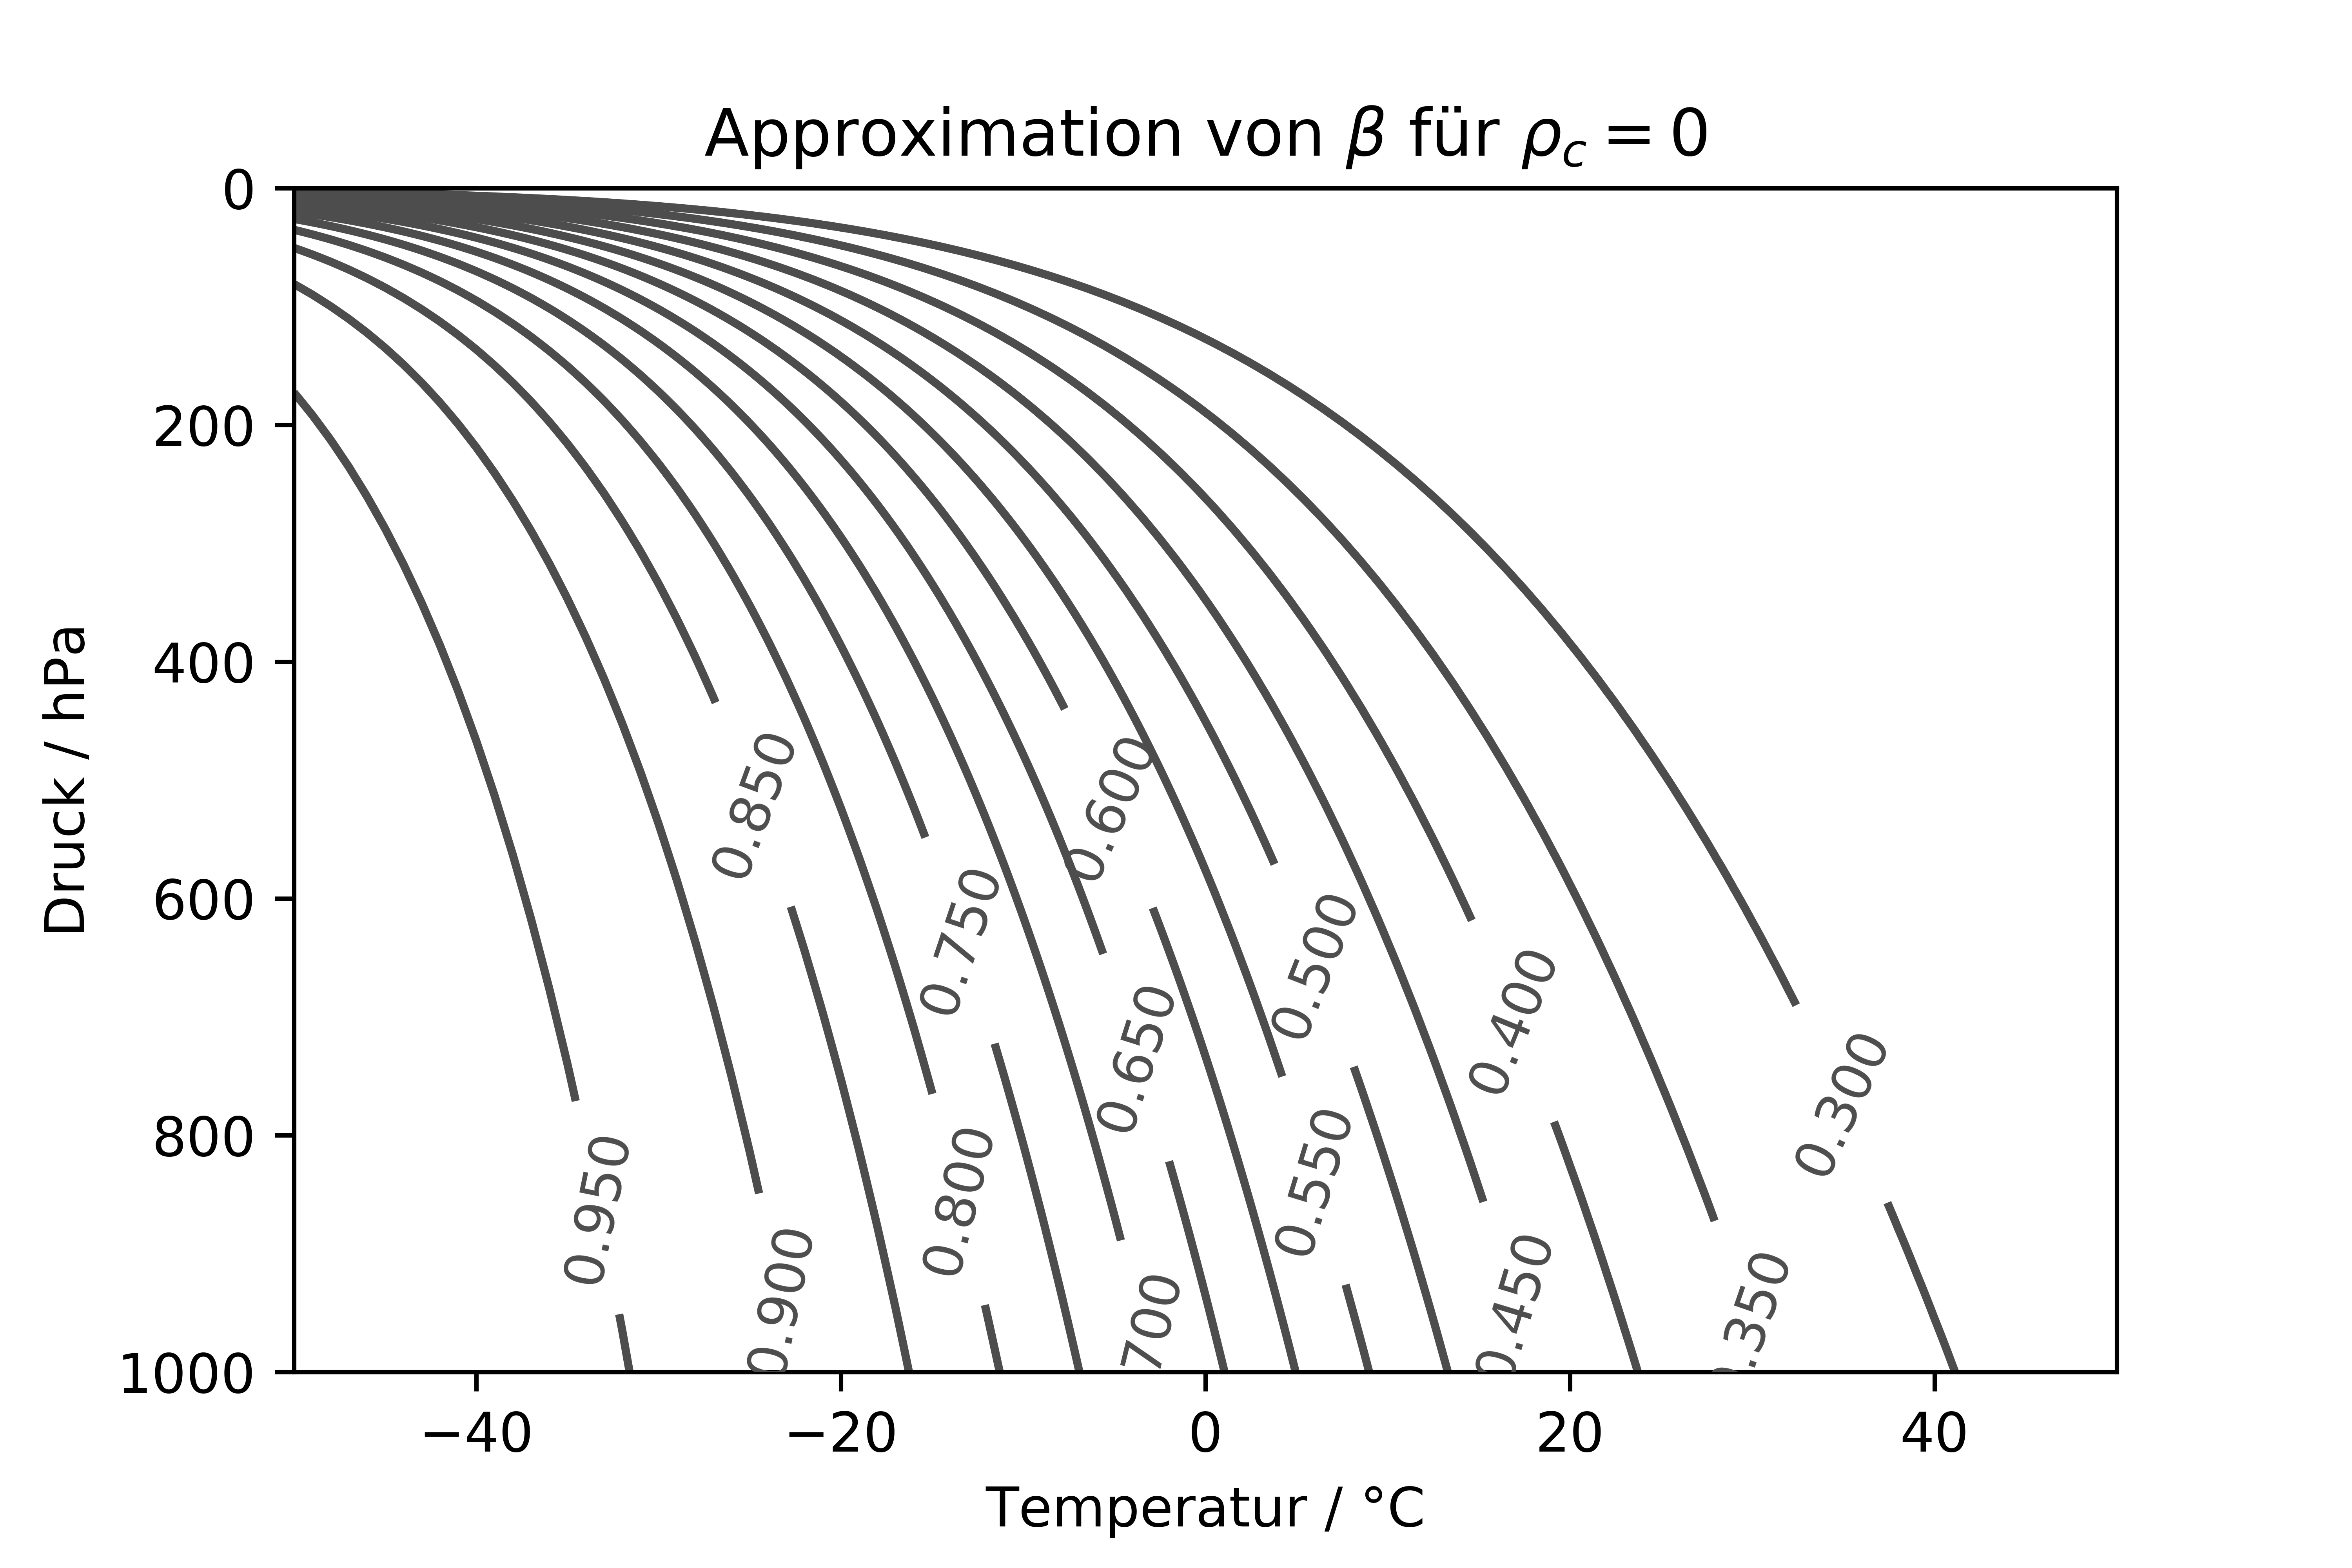
\includegraphics[width = .8\textwidth]{figs/beta_malr.png}
\caption{Approximation von $\beta$ gemäß Glg. \eqref{eq:beta_malr_approx}.}
\label{fig:beta_malr}
\end{figure}
%
Im Fall gesättigter Luft und
%
\begin{align}
\frac{\partial T}{\partial z}< - \Gamma_h
\end{align}
%
ist die Schichtung ebenfalls \textit{lokal instabil}.

\subsubsection{Aquivalentpotentielle Temperatur}
\label{sec:äquivalentpotentielle_temperatur}\index{äquivalentpotentielle Temperatur}\index{Temperatur!äquivalentpotentielle}

Um die sogenannte \textit{äquivalentpotentielle Temperatur}\index{äquivalentpotentielle Temperatur}\index{Temperatur!äquivalentpotentielle} $\theta_e$ (auch: pseudoäquivalentpotentielle Temperatur\index{pseudoäquivalentpotentielle Temperatur}\index{Temperatur!pseudoäquivalentpotentielle} oder seltener pseudopotentielle Temperatur\index{pseudopotentielle Temperatur}\index{Temperatur!pseudopotentielle}) eines Teilchens zu erhalten, sind zwei Schritte notwendig:
%
\begin{enumerate}
\item Hebe das Teilchen trockenadiabatisch auf sein LCL.
\item Hebe das Teilchen irreversibel-feuchtadiabatisch in eine unendliche Höhe. Die dann erhaltene potentielle Temperatur ist $\theta_e$.
\end{enumerate}
%
Diese Größe ist also nicht nur um den Druckunterschied, sondern auch um die vorhandene Feuchte, welche in Form von Phäsenübergangsenthalpie\index{Phäsenübergangsenthalpie} zu einer Temperaturerhöhung führen könnte, bereinigt. Sie eignet sich daher gut, um die Temperaturen verschiedener Luftmassen zu vergleichen.

\subsubsection{Reversibeläquivalentpotentielle Temperatur}
\label{sec:reversibeläquivalentpotentielle_temperatur}\index{reversibeläquivalentpotentielle Temperatur}\index{Temperatur!reversibeläquivalentpotentielle}

Die reversibeläquivalentpotentielle Temperatur\index{reversibeläquivalentpotentielle Temperatur}\index{Temperatur!reversibeläquivalentpotentielle} ist analog zur äquivalentpotentiellen Temperatur definiert, nur dass bei Schritt 2. aus Absch. \ref{sec:äquivalentpotentielle_temperatur} eine reversible Feuchtadiabate verfolgt wird.

\subsubsection{CAPE}
\label{sec:cape}\index{convective available potential Energy (CAPE)}\index{CAPE}\index{Energie!potentielle!konvektiv verfügbare}\index{potentielle Energie!konvektiv verfügbare}\index{konvektiv verfügbare potentielle Energie}

Die in diesem Abschnitt durchgeführten Herleitungen beziehen sich auf eine vertikale Luftsäule, wobei dynamische, d. h. durch das Geschwindigkeitsfeld entstehende Effekte, nicht berücksichtigt werden. Man definiert eine Funktion $f\left(z, z'\right)$ als die spezifische Kraft, also die Beschleunigung, die auf das Teilchen bei $z$ wirkt, wenn man es adiabatisch auf das Niveau $z'$ bringt und von einer hydrostatischen Atmosphäre ausgeht, also
%
\begin{align}
f\left(z, z'\right) \coloneqq -\frac{1}{\rho'\left(z, z'\right)}\frac{\partial p\left(z'\right)}{\partial z} - g = \frac{g\rho\left(z'\right)}{\rho'\left(z, z'\right)} - g = g\frac{\rho\left(z'\right) - \rho'\left(z, z'\right)}{\rho'\left(z, z'\right)}, 
\end{align}
%
wobei $\rho'\left(z, z'\right)$ die Dichte des Teilchens bei $z$ ist, nachdem man es adiabatisch nach $z'$ verschoben hat. Man definiert außerdem eine Funktion $\newtilde{F}\left(z, z'\right)$ durch
%
\begin{align}
\newtilde{F}\left(z, z'\right) \coloneqq g\int_{z}^{z'}\frac{\rho\left(z''\right) - \rho'\left(z, z''\right)}{\rho'\left(z, z''\right)}dz''
\end{align}
%
als die Arbeit, die die Schichtung an einem Teilchen geleistet hat, welches adiabatisch von $z$ nach $z'$ ausgelenkt wurde. Üblicherweise wählt man $z = z_{\text{2m}} \coloneqq Z_{\text{SFC}} + 2$ m, man definiert
%
\begin{align}
F\left(z\right) \coloneqq g\int_{z_{\text{2m}}}^{z}\frac{\rho\left(z'\right) - \rho'\left(z'\right)}{\rho'\left(z'\right)}dz'
\end{align}
%
mit dem Bezeichnungsmissbrauch
%
\begin{align}
\rho'\left(z'\right) \coloneqq \rho'\left(z_{\text{2m}}, z'\right).
\end{align}
%
Für den Integranden wird ebenso
%
\begin{align}
f\left(z'\right) \coloneqq g\frac{\rho\left(z'\right) - \rho'\left(z'\right)}{\rho'\left(z'\right)}\label{eq:uplift}
\end{align}
%
definiert. In Termen der Funktionen $F$ und $f$ lassen sich viele der üblicherweise im Zusammenhang mit Konvektion verwendeten Größen definieren. $z_T$ sei die als bekannt vorausgesetzte Tropopausenhöhe\index{Tropopausenhöhe}. Man definiert die sogenannte \textit{konvektiv verfügbare potentielle Energie}\index{convective available potential Energy (CAPE)}\index{CAPE}\index{Energie!potentielle!konvektiv verfügbare}\index{potentielle Energie!konvektiv verfügbare}\index{konvektiv verfügbare potentielle Energie} \textit{CAPE} durch
%
\begin{align}
\CAPE \coloneqq \int_{z_{\text{2m}}}^{z_T}\Theta\left(f\left(z'\right)\right)dz', \label{eq:def_cape}
\end{align}
%
wobei $\Theta$ die $\Theta-$Funktion bezeichnet\index{$\Theta-$Funktion}. Im Falle eines idealen Gases kann man für $f$ notieren
%
\begin{align}
f\left(z'\right) \coloneqq g\frac{\frac{1}{T} - \frac{1}{T'}}{\frac{1}{T'}} = g\frac{T' - T}{T} = g\frac{\theta' - \theta}{\theta}.
\end{align}
%
Im Fall feuchter Luft kann man $T \to T_v$ ersetzen, hierbei ist $T_v$ die in Glg. \eqref{eq:def_virtual_temperature} definierte virtuelle Temperatur, da bei dieser Temperatur die trockene Luft die gleiche Dichte hätte wie die vorhandene feuchte Luft\index{feuchte Luft}\index{Luft!feuchte}. Das \textit{level of free convection}\index{level of free convection}\index{LFC} $z_{\text{LFC}}$ ist die Höhe, in der das adiabatisch aufstegende Teilchen zum ersten mal leichter ist als die Umgebung
%
\begin{align}
z_{\text{LFC}} \coloneqq\inf\{z\newvline f\left(z\right) > 0\}.
\end{align}
%
Wenn das Teilchen diese Höhe erreicht, wird es weiter aufsteigen, was man als \index{freie Konvektion}\index{Konvektion!freie}\textit{freie Kovektion} bezeichnet, also Konvektion, die auch ohne dynamischen Antrieb stattfinden würde. Analog bezeichnet man
%
\begin{align}
z_{\text{EL}} \coloneqq\sup\{z\newvline f\left(z\right) > 0, z < 2z_T\}
\end{align}
%
als \index{Gleichgewichtsniveau}\textit{Gleichgewichtsniveau} \textit{(equilibrium level)}. Die tiefe Stratosphäre wurde sicherheitshalber ausgeklammert. Dies ist die Höhe, in der ein frei aufsteigendes Teilchen wieder schwerer wäre als seine Umgebung. Häufig wird in Glg. \eqref{eq:def_cape} die $\Theta-$Funktion weggelassen und nur von $z_{\text{LFC}}$ bist $z_{\text{EL}}$ integriert, was genau dann richtig ist, wenn in genau einem Höhenintervall thermische Labilität vorliegt, was häufig der Fall ist. Die \index{maximale Wolkenobergrenze}\index{Wolkenobergrenze!maximale}\textit{maximale Wolkenobergrenze} ist definiert als die Höhe, in der ein solches Teilchen seine kinetische Energie wieder verloren hätte, also
%
\begin{align}
z_{\text{MCT}} \coloneqq\inf\{z\newvline \newtilde{F}\left(z_{\text{LFC}}, z\right) < 0\}.
\end{align}
%
Das Phänomen $z_{\text{MCT}} > z_{\text{EL}}$ führt bei hochreichender Konvektion zur Ausprägung von Schichtungswellen\index{Schichtungswelle} an der Tropopause \textit{(overshooting tops)}\index{overshooting top}, was generell überall dort der Fall ist, wo ein stabil auf ein labil geschichtetes Höhenintervall folgt.

Hat ein Teilchen in zwei Metern Höhe die sogenannte \index{Auslösetemperatur}\textit{Auslösetemperatur} erreicht, kann es auch ohne dynamischen Antrieb in das LFC aufsteigen, also
%
\begin{align}
0 \equiv g\int_{z_{\text{2m}}}^{z_{\text{LFC}}}\frac{\rho\left(z'\right) - \newtilde{\rho}'\left(z'\right)}{\newtilde{\rho}'\left(z'\right)}, 
\end{align}
%
wobei $\newtilde{\rho}'\left(z'\right)$ die Dichte des adiabatisch von $z_{\text{2m}}$ nach $z'$ gehobenen Teilchens ist, was in zwei Metern Höhe die Auslösetemperatur hätte. Die Energie $\CIN$, die dabei überwunden werden muss, also
%
\begin{align}
\CIN \coloneqq \newtilde{F}\left(z_{\text{2m}}, z_{\text{LFC}}\right).
\end{align}
%
bezeichnet man als \textit{konvektive Schranke}\index{konvektive Schranke}\index{Schranke!konvektive} oder \textit{convective inhibition}\index{convective inhibition (CIN)}\index{CIN}. Die Höhe, in der ein auf die Auslösetemperatur aufgeheiztes Teilchen beim adiabatischen Aufstieg gesättigt wäre, bezeichnet man als \textit{convective condensation level (CCL)}\index{convective condensation level (CCL)}\index{Konvektionskondensationsniveau (KKN)}\index{KKN}\index{CCL}. Dies ist mindestens so groß wie das LCL, also
%
\begin{align}
z_{\text{CCL}} \geq z_{\text{LCL}}.
\end{align}

\chapter{\normalfont\textsc{Synoptik und Meso$-\alpha-$Sakla der Extratropen}}
\label{chap:synoptik_und_meso-alpha-skala_der_extratropen}\index{Synoptik!der Extratropen}\index{Skala!Mesoskala}\index{Mesoskala}\index{Skala!Meso$-\alpha-$Skala}\index{Meso$-\alpha-$Skala}

Die Gebiete zwischen den \index{Wendekreis}\textit{Wendekreisen}, die bei Breiten $\pm\beta$ liegen, werden als \index{Tropen}\textit{Tropen} bezeichnet, die Bereiche außerhalb dieses Streifens als \index{Extratropen}\textit{Extratropen}. Die Gebiete bei Breiten jenseits der \textit{Polarkreise}\index{Polarkreis}, die sich bei Breiten $\pm\left(\frac{\pi}{2} - \beta\right)$ befinden, werden als \index{Breiten!hohe}\index{hohe Breiten}\textit{hohe Breiten} bezeichnet. Die Bereiche zwischen den Tropen und den hohen Breiten bezeichnet man als \textit{mittlere Breiten}\index{mittlere Breiten}\index{Breiten!mittlere}. Die Dynamik der Extratropen unterscheidet sich wesentlich von der der Tropen, da in ersteren die diabatischen Flüsse durch die schwächere Konvektion und Strahlung kleiner sind und die geostrophische Annahme gerechtfertigter ist. Die Dynamik der Tropen enthält also gewisse Schwierigkeiten und wird daher separat in Kap. \ref{chap:tropische_dynamik} untersucht.

\section{Quasigeostrophie}
\label{sec:quasigeostrophie}\index{Quasigeostrophie}

Die Geostrophie gilt in nullter Ordnung auf der synoptischen Skala in den Extratropen, Folgerungen daraus wurden in Absch. \ref{sec:geostrophie} besprochen. In Absch. \ref{sec:barokline_instabilitaet} wurde bereits das quasigeostrophische Gleichungssystem, bestehend aus Tendenzgleichung Glg. \eqref{eq:tendency_eq_pre} und $\omega-$Gleichung Ggl. \eqref{eq:omega_eq}, abgeleitet, welches auf zonale Kanäle in den Extratropen angewandt werden kann, deren meridionale Ausdehnung eine Anwendung der $\beta-$Ebenen-Approximation erlaubt. Es wurde gezeigt, dass die baroklinen Wellen, die man als Lösungen eines quasigeostrophischen linearisierten Zweischichtmodells findet, instabil sind. Der hierdurch angestoßene Prozess ist die Zyklogenese, was hier näher behandelt werden soll. Man definiert zunächst die \index{Geopotentialtendenz}\textit{Geopotentialtendenz}\index{Tendenz!des Geopotentials} durch
%
\begin{align}
\chi \coloneqq \frac{\partial\phi}{\partial t}, \label{sec:tendency_def}
\end{align}
%
\subsection{Tendenzgleichung}
\label{sec:tendenzgleichung}\index{Tendenzgleichung}

Mit Glg. \eqref{sec:tendency_def} kann man Glg. \eqref{eq:tendency_eq_pre} wie folgt umschreiben:
%
\begin{align}
\underbrace{\vphantom{\left[\Delta + \frac{f_0^2}{\sigma}\frac{\partial^2}{\partial p^2}\right]\chi = -f_0v_g\beta - \mathbf{v}_{h, g}\cdot\nabla\left(\Delta\phi\right) - \frac{f_0^2}{\sigma}\frac{\partial}{\partial p}\left[\mathbf{v}_{h, g}\cdot\nabla\frac{\partial\phi}{\partial p}\right]}\left[\Delta + \frac{f_0^2}{\sigma}\frac{\partial^2}{\partial p^2}\right]\chi}_{=:A} = \underbrace{\vphantom{\left[\Delta + \frac{f_0^2}{\sigma}\frac{\partial^2}{\partial p^2}\right]\chi = -f_0v_g\beta - \mathbf{v}_{h, g}\cdot\nabla\left(\Delta\phi\right) - \frac{f_0^2}{\sigma}\frac{\partial}{\partial p}\left[\mathbf{v}_{h, g}\cdot\nabla\frac{\partial\phi}{\partial p}\right]} -f_0v_g\beta}_{=:B}\underbrace{\vphantom{\left[\Delta + \frac{f_0^2}{\sigma}\frac{\partial^2}{\partial p^2}\right]\chi = -f_0v_g\beta - \mathbf{v}_{h, g}\cdot\nabla\left(\Delta\phi\right) - \frac{f_0^2}{\sigma}\frac{\partial}{\partial p}\left[\mathbf{v}_{h, g}\cdot\nabla\frac{\partial\phi}{\partial p}\right]} -\mathbf{v}_{h, g}\cdot\nabla\left(\Delta\phi\right)}_{=:C} \underbrace{\vphantom{\left[\Delta + \frac{f_0^2}{\sigma}\frac{\partial^2}{\partial p^2}\right]\chi = -f_0v_g\beta - \mathbf{v}_{h, g}\cdot\nabla\left(\Delta\phi\right) - \frac{f_0^2}{\sigma}\frac{\partial}{\partial p}\left[\mathbf{v}_{h, g}\cdot\nabla\frac{\partial\phi}{\partial p}\right]} -\frac{f_0^2}{\sigma}\frac{\partial}{\partial p}\left[\mathbf{v}_h\cdot\nabla\frac{\partial\phi}{\partial p}\right]}_{=:D}\label{eq:tendency_eq_cyclogen}
\end{align}
%
Dabei wurde im Term D eine Ableitung nach $p$ herausgezogen, wobei Glg. \eqref{eq:therm_wind} ausgenutzt wurde, da dies den Term anschaulicher macht. Diese Gleichung soll nun konzeptionell untersucht werden. Geht man davon aus, dass $\chi$ aus nur einer einzigen Fourier-Komponente im dreidimensionalen Raum besteht, folgt
%
\begin{align}
\text{A} \sim -\chi \sim \text{Zyklogenese}, 
\end{align}
%
\index{Zyklogenese} wobei mit Zyklogenese hier ein Absinken der Druckfläche gemeint ist. In den Extratropen findet man häufig meridionale Wellen, die einem zonalen Grundstrom $U$ überlagert sind, daher macht man für das Geopotential $\phi$ den Ansatz
%
\begin{align}
\phi\left(x, y, p\right) = -Uf_0y + \frac{\newhat{v}f_0L}{2\pi}\sin\left(\frac{2\pi}{L}x\right)\sin\left(ap + b\right) + \phi_0\left(p\right), 
\end{align}
%
wobei $\newhat{v}$ die Geschwindigkeitsamplitude der meridionalen Schwingung bezeichnet. Die linere Funktion $ap + b$ ermöglicht eine Phasenverschiebung der Störung mit der Höhe; $\varphi_0$ steht für einen Hintergrundzustand. Für den Term $B$ findet man in diesem Fall
%
\begin{align}
B = -f_0\beta\newhat{v}\cos\left(\frac{2\pi}{L}x\right).
\end{align}
%
Dieser Term führt also überall dort zu Zyklogenese, wo $v_g$ negativ ist, also stromaufwärts des Troges und stromabwärts des Rückens. Er trägt also zu retrograder Progression bei. Term $B$ ist die Advektion planetarer Vorticity. Für den Ausdruck C, welcher die Advektion relativer Vorticity ist, berechnet man zunächst
%
\begin{align}
\Delta\phi = -\frac{2\pi}{L}\newhat{v}f_0\sin\left(\frac{2\pi}{L}x\right), 
\end{align}
%
wobei daran erinnert sei, dass $\Delta\phi$ sich hier nur auf die Horizontale bezieht. Hieraus folgt
%
\begin{align}
C = U\frac{4\pi^2}{L^2}\newhat{v}f_0\cos\left(\frac{2\pi}{L}x\right) = -\frac{2\pi U}{L\beta}B.
\end{align}
%
Dieser Term führt also stromabwärts des Troges und stromaufwärts des Rückens zu Zyklogenese, anderswo zu Antizyklogenese\index{Antizyklogenese}. Er trägt also zu normaler Progression bei und nimmt mit der Wellenlänge ab. Bei einer Grenzwellenlänge
%
\begin{align}
\newtilde{L} = \frac{2\pi U}{\beta}
\end{align}
%
kompensieren sich $B$ und $C$, die Welle ist stationär. Noch längere Wellen propagieren retrograd. Beide Terme $B$ und $C$ verschwinden an den Achsen der Druckgebilde, also tragen sie ausschließlich zu deren Verlagerung bei, nicht jedoch zu ihrer Vertiefung. Hierfür ist der Term $D$ zuständig. Das Skalarprodukt $\mathbf{v}_h\cdot\nabla\frac{\partial\phi}{\partial p}$ ist die horizontale Temperaturadvektion, wie sich aus der hydrostatischen Grundgleichung in der Form Glg. \eqref{eq:hydrostatic_p} ergibt. Daher bezeichnet man $D$ auch als negative \textit{differenzielle Temperaturadvektion}\index{differenzielle Temperaturadvektion}\index{Temperaturadvektion!differenzielle}. Es gilt
%
\begin{align}
D = \begin{cases}
\text{postiv, falls Kaltluftadvektion mit der Tiefe zunimmt, }\\
\text{negativ, falls Warmluftadvektion mit der Tiefe zunimmt.}
\end{cases}
\end{align}
%
Warmluftadvektion in der Höhe und Kaltluftadvektion in der Tiefe führt also zu Zyklogenese, während Kaltluftadvektion in der Höhe und Warmluftadvektion in der Tiefe zu Antizyklogenese führt. Dies ist anschaulich, da wärmere Luft ein größeres spezifisches Volumen hat.

\subsection{$\omega-$Gleichung}
\label{sec:omegagleichung}\index{$\omega-$Gleichung}

\section{Semigeostrophie}
\label{sec:semigeostrophie}\index{Semigeostrophie}

Die semigeostrophische Annahme ist eine Relaxation der quasigeostrophischen Annahme. Als Teil des Lösungsspektrums erhält man Flächen im Raum besonderer Baroklinität, sogenannte \textit{Fronten}\index{Front}.

\section{PV-Denken}
\label{sec:pv-denken}\index{PV-Denken}\index{potentielle Vorticitiy}\index{Vorticity!potentielle}

\chapter{\normalfont\textsc{Tropische Dynamik}}
\label{chap:tropische_dynamik}\index{Dynamik!tropische}

\section{Skalenanalyse}
\label{sec:skalenanalyse}\index{Skalenanalyse!Tropen}

\section{Zyklogenese}
\label{sec:zyklogenese}\index{Zyklogenese}

\chapter{\normalfont\textsc{Turbulenz}}
\label{chap:turbulenz}\index{Turbulenz}

Es gibt keine mathematisch exakte Definition dafür, ob ein Strömungsfeld turbulent ist oder nicht. Es kann davon ausgegangen werden, dass jedes Strömungsfeld, wenn man es nur aus genügend großer Entfernung betrachtet, tubulent aussieht. Zoomt man jedoch weit genug hinein, wird man meistens eine Skala finden, auf der des Feld einen \textit{laminaren}\index{laminare Strömung}\index{Strömung!laminare} Eindruck macht, was man als das Gegenteil von Turbulenz versteht. Ist diese Skala die molekulare Skala, liegt \textit{volle Turbulenz}\index{Turbulenz!volle}\index{volle Turbulenz} vor. 

\section{Grundlagen}
\label{sec:grundlagen}

Definiere einen Mittelungsoperator durch
%
\begin{align}
\newoverline{f} \coloneqq \frac{1}{\mu\left(\Omega\right)}\int_\Omega fd\omega,\label{eq:simple_average}
\end{align}
%
wobei $\Omega$ eine beliebeige räumliche und/oder zeitliche Menge sein soll, $\mu\left(\Omega\right)$ deren Maß, $f$ eine beliebige Funktion von Ort und Zeit und $d\omega$ ein geeignetes differenzial. Nun kann man $f$ in der Form
%
\begin{align}
f & \equiv \newoverline{f} + f'
\end{align}
%
zerlegen; hierzu definiert man die Fluktuation oder Turbulenz durch
%
\begin{align}
f' &\coloneqq f - \newoverline{f}.
\end{align}
%
Wenn die Aussagen
%
\begin{align}
\newoverline{\frac{\partial f}{\partial x_i}} & = \frac{\partial\newoverline{f}}{\partial x_i}, \label{eq:reynolds_prop_1}\\
\newoverline{\frac{\partial f}{\partial t}} & = \frac{\partial\newoverline{f}}{\partial t}, \label{eq:reynolds_prop_2}\\
\newoverline{f'\newoverline{g}} & = 0\label{eq:reynolds_prop_3}
\end{align}
%
mit einem beliebigen Feld $g$ gelten, bezeichnet man $\newoverline{f}$ als \index{Reynolds-Operator}\textit{Reynolds-Operator} und die entsprechende Mittelung als \index{Reynolds-Mittelung}\textit{Reynolds-Mittelung}. Man macht sich leicht klar, dass hieraus auch die beiden Aussagen
%
\begin{align}
\newoverline{f'} = 0, && \newoverline{\newoverline{f}} = \newoverline{f}
\end{align}
%
folgen. Man kümmert sich an dieser Stelle nicht darum, wie ein solcher Operator konkret aussehen könnte, in Absch. \ref{sec:konkrete_mittelungsoperatoren} wird festgestellt werden, dass die üblichen Mittelungsoperatoren keine Reynolds-Operatoren sind. Von nun an wird jedoch nicht mehr Glg. \eqref{eq:simple_average} verwendet, anstattdessen wird das \textit{Hesselberg-Mittel}\index{Hesselberg-Mittel}
%
\begin{align}
\left\langle f\right\rangle \coloneqq \frac{1}{\int_\Omega\rho d\omega}\int_\Omega\rho fd\omega\label{eq:hesselberg-average}
\end{align}
%
genutzt, wobei $\rho$ die Dichte ist. Für die Fluktuation schreibt man nun
%
\begin{align}
f'' \coloneqq f - \left\langle f\right\rangle.
\end{align}
%
Man nimmt nun an, dass das Hesselberg-Mittel\index{Hesselberg-Mittel} ein Reynolds-Operator\index{Reynolds-Operator} ist. Wendet man dies auf das trockenadiabatische Gleichungssystem an, folgt
%
\begin{align}
\frac{\partial\newoverline{\mathbf{v}}}{\partial t} & = -\left(\newoverline{\mathbf{v}}\cdot\nabla\right)\newoverline{\mathbf{v}} - \newoverline{\left(\mathbf{v}''\cdot\nabla\right)\mathbf{v}''} - \newoverline{\alpha}\frac{\partial\newoverline{p}}{\partial x} - \newoverline{\alpha''\frac{\partial p'}{\partial x}} - \mathbf{f}\times\newoverline{\mathbf{v}} + \mathbf{g},\\
\frac{\partial\newoverline{\theta}}{\partial t}& = -\newoverline{\mathbf{v}}\cdot\nabla\newoverline{\theta} - \newoverline{\mathbf{v}''\cdot\nabla\theta''} ,\\
\frac{\partial\newoverline{\rho}}{\partial t} & = -\newoverline{\rho}\nabla\cdot\newoverline{\mathbf{v}} - \newoverline{\mathbf{v}}\cdot\nabla\newoverline{\rho} - \newoverline{\rho''\nabla\cdot\mathbf{v}''} - \newoverline{\mathbf{v}''\cdot\nabla\rho''},\\
\newoverline{p}\newoverline{\alpha}& = R_d\newoverline{T} - \newoverline{p''\alpha''}.
\end{align}
%
Die prognostischen Gleichungen der gemittelten Felder sind also gegenüber denen der ungemittelten Felder um Terme der Form $\newoverline{f''g''}$ korrigiert, wobei $f, g$ linear in den Feldern und ihren Ableitungen sind. Diese Terme bezeichnet man als die Konvergenzen der \textit{turbulenten Korrelationsflüsse}\index{Korrelationsfluss}. Diese sind natürlich von der Größe der Menge abhängig, über die gemittelt wird, d. h. im Falle eines numerischen Modells auflösungsabhängig. Im Falle einer immer kleiner werdenden Mittelungsmege verlieren die Kovarianzterme an Bedeutung, bis sie schließlich ganz verschwinden. 

Für die turbulenten Größen liegen jedoch keine prognostischen Gleichungen vor, was man als \textit{Schließungsproblem}\index{Schließungsproblem} bezeichnet. Um die Korrelationsterme in der Impulsgleichung näher zu spezifizieren, wendet man den Reynolds-Mittelungsoperator auf Glg. \eqref{eq:momentum_flux_form} an, man erhält so
%
\begin{align}
\frac{\partial\left(\rho\mathbf{v}\right)}{\partial t} + \nabla p + \nabla\cdot\overleftrightarrow{\Pi} - \rho\mathbf{g} + \nabla\cdot\overleftrightarrow{\newtilde{\Pi}} = \mathbf{0}, 
\end{align}
%
wobei die Horizontalstriche der Übersichtlichkeit halber weggelassen wurden. Außerdem ist der \index{Turbulenzkorrelationstensor}\textit{Turbulenzkorrelationstensor} $\newtilde{\Pi}$ durch
%
\begin{align}
\newtilde{\Pi} \coloneqq \rho\left(\begin{array}{ccc}
\newoverline{u''u''} & \newoverline{u''v''} & \newoverline{u''w''} \\
\newoverline{v''u''} & \newoverline{v''v''} & \newoverline{v''w''} \\
\newoverline{w''u''} & \newoverline{w''v''} & \newoverline{w''w''}
\end{array}\right) =: \left(\begin{array}{ccc}
\newtilde{\Pi}_{x, x} & \newtilde{\Pi}_{x, y} & \newtilde{\Pi}_{x, z} \\
\newtilde{\Pi}_{y, x} & \newtilde{\Pi}_{y, y} & \newtilde{\Pi}_{y, z} \\
\newtilde{\Pi}_{z, x} & \newtilde{\Pi}_{z, y} & \newtilde{\Pi}_{z, z}
\end{array}\right)
\end{align}
%
definiert. Es wurde von der gerechtfertigten Annahme
%
\begin{align}
\left|\frac{\rho''}{\newoverline{\rho}}\right| \ll \left|\frac{u''}{\newoverline{u}}\right|
\end{align}
%
ausgegangen. $-\nabla\cdot\newtilde{\Pi}$ liefert die \textit{Eddy-Stress-Terme}\index{Eddy-Stress-Term}, die sich in der Impulsgleichung niederschlagen und anstatt der $- \newoverline{\left(\mathbf{v}''\cdot\nabla\right)\mathbf{v}''} - \newoverline{\alpha''\frac{\partial p''}{\partial x}}$ verwendet werden.

\subsection{Turbulente Dissipation}
\label{sec:turbulente_dissipation}\index{turbulente Dissipation}\index{Dissipation!turbulente}

Man kann analog zur molekularen Dissipation $\epsilon$ (s. Glg. \eqref{eq:dissipation}) eine mit der Turbulenz verbundene \textit{turbulente Dissipation}\index{turbulente Dissipation}\index{Dissipation!turbulente}
%
\begin{center}
\doublebox{\parbox{\textwidth}{
\begin{center}
\begin{align}
\epsilon_\text{turb} \coloneqq \frac{1}{\rho}\sum_{i, j = 1}^3-\newtilde{\Pi}_{i, j}S_{i, j} = \frac{1}{\rho}\sum_{i, j = 1}^3-\newtilde{\Pi}_{i, j}\frac{\partial v_j}{\partial x_i}
\end{align}
\end{center}
}}
\end{center}
%
definieren. Da für $\overleftrightarrow{\newtilde{\Pi}}$ keine explizite Formel vorliegt, kann man kein turbulentes Analogon zu Glg. \eqref{eq:dissipation_sign} finden: Das Vorzeichen von $\epsilon_\text{turb}$ bleibt unbestimmt.

\subsection{Konkrete Mittelungsoperatoren}
\label{sec:konkrete_mittelungsoperatoren}

Sei $f$ eine skalare oder vektorielle Funktion von Ort und Zeit. Ein allgemeiner Mittelungsoperator $\newoverline{f}$ wird definiert durch
%
\begin{align}
\newoverline{f}\left(x_i\right) \coloneqq \frac{\int_\Omega f\left(x_i\right)h\left(x_i\right)dx_1\dotsc dx_n}{\int_\Omega h\left(x_i\right)dx_1\dotsc dx_n}, \label{eq:av_op_gen}
\end{align}
%
wobei die Zeit $t$ als eine der $x_i$ aufgefasst werden soll und $h$ eine Gewichtungsfunktion darstellt.

\subsubsection{Gleitendes Zeitmittel}
\label{sec:gleitendes_zeitmittel}\index{gleitendes Zeitmittel}\index{Mittel!gleitendes}

Das \textit{gleitende Zeitmittel} mit der Mittelungslänge $T$ erhält man aus Glg. \eqref{eq:av_op_gen} mit $\Omega = \left(t - \frac{T}{2}, t + \frac{T}{2}\right)$ und $h = 1$, also
%
\begin{align}
\newoverline{f}\left(\mathbf{r}, t\right) = \frac{1}{T}\int_{t-\frac{T}{2}}^{t + \frac{T}{2}}f\left(\mathbf{r}, t'\right)dt'.
\end{align}
%
Man überpruft nun, ob dieser Operator die Eigenschaften eines Reynolds-Operators Glg.en \eqref{eq:reynolds_prop_1} - \eqref{eq:reynolds_prop_3} erfüllt. Zunächst gilt
%
\begin{align}
\frac{\partial\overline{f}}{\partial x_i} & = \frac{1}{T}\int_{t-\frac{T}{2}}^{t + \frac{T}{2}}\frac{\partial f}{\partial x_i}\left(\mathbf{r}, t'\right)dt' = \newoverline{\frac{\partial f}{\partial x_i}}, 
\end{align}
%
Glg. \eqref{eq:reynolds_prop_1} ist also erfüllt. Die Überprüfung der Erfüllung von Glg. \eqref{eq:reynolds_prop_2} erfolgt mittels des Haupsatz der Differenzial- und Integralrechnung:
%
\begin{align}
\frac{\partial\overline{f}}{\partial t} & = \frac{f\left(\mathbf{r}, t + \frac{T}{2}\right) - f\left(\mathbf{r}, t - \frac{T}{2}\right)}{T} = \frac{1}{T}\int_{t-\frac{T}{2}}^{t + \frac{T}{2}}\frac{\partial f}{\partial t'}\left(\mathbf{r}, t'\right)dt' = \newoverline{\frac{\partial f}{\partial t}}
\end{align}
%
Die ersten beiden Eigenschaften sind also erfüllt. Für die dritte rechnet man mit $g = 1$
%
\begin{align}
\newoverline{f'} & = \frac{1}{T}\int_{t-\frac{T}{2}}^{t + \frac{T}{2}}f\left(\mathbf{r}, t'\right) - \newoverline{f}\left(\mathbf{r}, t'\right)dt' \hastobe 0.
\end{align}
%
Dies soll für beliebige Zeitpunkte gelten, also folgt hieraus bereits
%
\begin{align}
\newoverline{f} = f
\end{align}
%
zu allen Zeitpunkten als Kriterium für die Gültigkeit von Glg. \eqref{eq:reynolds_prop_3} für den einfachen Fall $g = 1$, was nur für lineare Funktionen $f$ der Fall ist.

\subsubsection{Hesselberg-Mittel}
\label{sec:hesselberg-mittel}\index{Hesselberg-Mittel}

Setzt man in Glg. \eqref{eq:av_op_gen} den Fall $h = \rho$ ein, erhält man das bereits in der Einleitung erwähnte Hesselberg-Mittel\index{Hesselberg-Mittel}. Für dieses notiert man die Zerlegung
%
\begin{align}
f = \left\langle f\right\rangle + f'',
\end{align}
%
um das Hesselberg-Mittel\index{Hesselberg-Mittel} von anderen Mittelungen wie z. B. dem gleitenden Zeitmittel\index{gleitendes Zeitmittel}\index{Mittel!gleitendes} oder einem allgemeinen Reynolds-Operator abzugrenzen.

\subsubsection{Tiefpass}
\label{sec:tiefpass}\index{Tiefpass}

Die Fourier-Transformation\index{Fourier-Transformation} $\newtilde{f}\left(k\right)$ eines Feldes $f = f\left(x\right)$ lautet
%
\begin{align}
\newtilde{f}\left(k\right) \stackrel{\text{Glg. \eqref{eq:def_ft_1d}}}{=} C\int_{-\infty}^\infty f\left(x\right)\exp\left(-ikx\right)dx.
\end{align}
%
Die inverse Fourier-Transformation ist laut Glg. \eqref{eq:def_ft_1d_inv} gegeben durch
%
\begin{align}
f\left(x\right) = \newtilde{C}\int_{-\infty}^\infty f\left(x\right)\exp\left(ikx\right)dk,
\end{align}
%
wobei laut Glg. \eqref{eq:ft_norm} auf $C\newtilde{C} = 1/\left(2\pi\right)$ zu achten ist. Ein Tiefpass\index{Tiefpass} mit der Grenz-Wellenzahl $k^\star > 0$ wird durch die Gleichung
%
\begin{align}
\newoverline{f}\left(x\right) = \newtilde{C}\int_{-k^\star}^{k^\star}f\left(x\right)\exp\left(ikx\right)dk
\end{align}
%
festgelegt. Wie schon durch die Notation $\newoverline{f}$ angedeutet wurde, handelt es sich auch hier um eine Art Mittelungsoperator\index{Mittelungsoperator}. Für die Fluktuation\index{Fluktuation} $f'$ erhält man
%
\begin{align}
f'\left(x\right) &\coloneqq f\left(x\right) - \newoverline{f}\left(x\right) = \newtilde{C}\int_{-\infty}^{\infty}f\left(x\right)\exp\left(ikx\right)dk - \newtilde{C}\int_{-k^\star}^{k^\star}f\left(x\right)\exp\left(ikx\right)dk\nonumber\\
& = \newtilde{C}\int_{-\infty}^{-k^\star}f\left(x\right)\exp\left(ikx\right)dk + \newtilde{C}\int_{k^\star}^{\infty}f\left(x\right)\exp\left(ikx\right)dk.
\end{align}


\section{Mischungswegansatz}
\label{sec:mischungswegansatz}\index{Mischungswegansatz}

Die $\tau_{i, j}$ sind jedoch immernoch unbekannte Größen, um diese zu parametrisieren\index{Parametrisierung} (s. hierzu auch Absch. \ref{sec:parametrisierungen}), verwendet man den \index{Mischungsweg}\textit{Mischungswegansatz}. Hierbei geht man davon aus, dass Druckgradient und Coriolis-Kraft keine bedeutende Rolle spielen, woraus
%
\begin{align}
\md{\mathbf{v}} = \mathbf{0}\label{eq:burgers_eq}
\end{align}
%
folgt, was man als \textit{Burgers-Gleichung}\index{Burgers-Gleichung} bezeichnet. Ihr entsprechend bewegt sich jedes Fluidteilchen auf einer geradlinig-gleichförmigen Bahn. Dies ist jedoch kein vollständig sinnvoller Ansatz, es ergibt sich daraus jedoch eine sinnvolle Möglichkeit, die $u'', v'', w''$ zu parametrisieren. Bewegt sich ein Teilchen von $z$ nach $z + l$ und behält dabei seine Horizontalgeschwindigkeit $\mathbf{v}_h$ bei, gilt nach Glg. \eqref{eq:burgers_eq}
%
\begin{align}
\mathbf{v}_h''\left(z + l\right) = \mathbf{v}_h\left(z + l\right) - \overline{\mathbf{v}_h}\left(z + l\right) = \newoverline{\mathbf{v}_h}\left(z\right) - \overline{\mathbf{v}_h}\left(z + l\right) = \overline{\mathbf{v}_h}\left(z + l\right) - l\frac{\partial\newoverline{\mathbf{v}_h}}{\partial z} - \overline{\mathbf{v}_h}\left(z + l\right) = -l\frac{\partial\newoverline{\mathbf{v}_h}}{\partial z}
\end{align}
%
Man beachte hierbei auch das Vorzeichen von $l$, welches im Fall nach unten gerichteter Bewegung als negativ verstanden werden muss. Somit folgt beispielsweise
%
\begin{align}
\tau_{x, z} = -\rho\newoverline{u''w''} = \rho\newoverline{w''l}\frac{\partial\newoverline{u}}{\partial z}.
\end{align}
%
Im Falle einer indifferent geschichteten Atmosphäre gilt $\left|w''\right| \sim \left|\mathbf{v}_h''\right|$, was der Tatsache entspricht, dass in diesem Fall die horizontale Skala der Wirbel genauso groß ist wie die vertikale, man setzt daher
%
\begin{align}
w'' = l\left|\frac{\partial\overline{\mathbf{v}_h}}{\partial z}\right|.
\end{align}
%
Daraus folgt
%
\begin{align}
\tau_{x, z} = -\rho\newoverline{u'w'} = \rho\newoverline{l^2}\left|\frac{\partial\newoverline{\mathbf{v}_h}}{\partial z}\right|\frac{\partial\newoverline{u}}{\partial z} \equiv A_z\frac{\partial\overline{u}}{\partial z}.\label{eq:eddy_corr_para}
\end{align}
%
Den Koeffizienten
\begin{align}
A_z \coloneqq \rho\newoverline{l^2}\left|\frac{\partial\newoverline{\mathbf{v}_h}}{\partial z}\right|\label{eq:def_eddy_exchange_coeff}
\end{align}
%
bezeichnet man als \index{Eddy-Austauschkoeffizient}\textit{Eddy-Austauschkoeffizienten}.

\subsection{Planetarische Grenzschicht}
\label{sec:planetarische_Grenzschicht}\index{planetarische Grenzschicht}\index{Grenzschicht!planetarische}

Die \textit{planetarische Grenzschicht}\index{planetarische Grenzschicht}\index{Grenzschicht!planetarische} ist definiert als diejenige untere Schicht der Atmosphäre, in der die \index{Bodenreibung}\textit{Bodenreibung}, d. h. die Existenz der Erdoberfläche, einen Einfluss hat. Als Kräftegleichgewicht setzt man hier an
%
\begin{align}
-fv & = -\frac{1}{\rho}\frac{\partial p}{\partial x} + \frac{1}{\rho}\frac{\partial\tau_{x, z}}{\partial z}, \label{eq:friction_boundary_equilibrium_x}\\
fu & = -\frac{1}{\rho}\frac{\partial p}{\partial y} + \frac{1}{\rho}\frac{\partial\tau_{y, z}}{\partial z}.\label{eq:friction_boundary_equilibrium_y}
\end{align}
%
wobei die Mittelungsoperatoren der Übersichtlichkeit halber wieder weggelassen wurden. Ebenfalls unterschlagen wurden an dieser Stelle die horizontalen Korrelationsflüsse. Geht man außerdem davon aus, dass die Dichte innerhalb des betrachteten Höhenintervalls nur wenig variiert, folgt
%
\begin{align}
-fv & = -\frac{1}{\rho}\frac{\partial p}{\partial x} + \frac{\partial}{\partial z}\left(\frac{\tau_{x, z}}{\rho}\right), \label{eq:momentum_tau_z_ind_x}\\
fu & = -\frac{1}{\rho}\frac{\partial p}{\partial y} + \frac{\partial}{\partial z}\left(\frac{\tau_{y, z}}{\rho}\right)\label{eq:momentum_tau_z_ind_y}.
\end{align}
%
Man nimmt nun an, dass die Bewegung nur eine x-Komponente hat und definiert die sogenannte \textit{Reibungsgeschwindigkeit}\index{Reibungsgeschwindigkeit} $u_\star > 0$ durch
%
\begin{align}
u_\star^2 \coloneqq \frac{\tau_{x, z}}{\rho} = \frac{A_z}{\rho}\frac{\partial\overline{u}}{\partial z}
\end{align}
%
Bisher wurde angenommen, dass die Mischungsweglänge $l$ höhenunabhängig ist. Sehr nahe an der Erdoberfläche ist jedoch zu erwarten, dass die vertikale Ausdehung der Wirbel mit der Höhe zunimmt, was man im einfachsten Fal über
%
\begin{align}
l\left(z\right) = kz\label{eq:karman_eq}
\end{align}
%
ausdrücken kann, wobei die Zahl $k > 0$ als \textit{von Karman-Konstante}\index{von Karman-Konstante} bezeichnet wird. Diese hat einen typischen Wert von $0, 4$. Glg. \eqref{eq:karman_eq} ist nur bis zu einer gewissen Höhe gültig. Somit folgt
%
\begin{align}
u_\star^2 = k^2z^2\left|\frac{\partial\newoverline{u}}{\partial z}\right|^2, 
\end{align}
%
also im Fall $\frac{\partial\newoverline{u}}{\partial z} > 0$
%
\begin{align}
u_\star = kz\frac{\partial\newoverline{u}}{\partial z}.
\end{align}
%
Die Lösung für $\newoverline{u}\left(z\right)$ ist das logarithmische Windprofil
%
\begin{center}
\doublebox{\parbox{\textwidth}{
\begin{center}
\begin{align}
\newoverline{u}\left(z\right) = \frac{u_\star}{k}\ln\left(\frac{z}{z_0}\right).\label{eq:ln_wind_profile}
\end{align}
\end{center}
}}
\end{center}
%
Die Konstante $z_0 > 0$ ist die \textit{Rauhigkeitslänge}\index{Rauhigkeitslänge}, es gilt $\newoverline{u}\left(z_0\right) = 0$. Glg. \eqref{eq:ln_wind_profile} sollte überhaupt nur für $z > z_0$ angewandt werden.

Die Schicht, in der Ggl. \eqref{eq:karman_eq} eine gute Approximation ist, bezeichnet man als \textit{Prandtl-Schicht}\index{Prandtl-Schicht}. Sie hat typischerweise Ausdehungen von ein bis zwei freien Mischungsweglängen $l$. Nach unten hin ist sie begrenzt durch die \index{laminare Unterschicht}\index{Unterschicht!laminare}\textit{laminare Unterschicht}, welche im Bereich $\sim 1$ mm dick ist und in welcher molekulare Diffusion vorherrscht. Laminare Unterschicht und Prandtl-Schicht zusammengenommen bilden die \index{Oberflächenschicht}\textit{Oberflächenschicht}. Nach oben hin ist die Oberflächenschicht durch die \index{Ekman-Schicht}\textit{Ekman-Schicht} begrenzt.

\section{Ekman-Transport}
\label{sec:ekman-transport}\index{Ekman-Transport}

Der \textit{Ekman-Transport} tritt überall dort auf, wo ein geostrophisches Medium auf eine horizontale Begrenzung trifft, an der die Adhäsionsbedingung\index{Adhäsionsbedingung} gilt. Definiert man den \textit{Eddy-Viskositäts-Koeffizienten}\index{Eddy-Viskositäts-Koeffizient} $K$ durch
%
\begin{align}
K \coloneqq \frac{A_z}{\rho}, 
\end{align}
%
schreibt sich Glg. \eqref{eq:eddy_corr_para} als
%
\begin{align}
\tau_{x, z} = K\rho\frac{\partial\newoverline{u}}{\partial z}.
\end{align}
%
Unter der Voraussetzung $\frac{\partial}{\partial z}\left(K\rho\right) = 0$, was nur oberhalb der Prandtl-Schicht\index{Prandtl-Schicht} eine brauchbare Annahme ist, gilt
%
\begin{align}
\frac{1}{\rho}\frac{\partial\tau_{x, z}}{\partial z} = K\frac{\partial^2\newoverline{u}}{\partial z^2}.
\end{align}
%
Die Glg.en \eqref{eq:friction_boundary_equilibrium_x} - \eqref{eq:friction_boundary_equilibrium_y} werden dann zu
%
\begin{align}
0 = f\newtilde{v}+ K\frac{\partial^2\newoverline{u}}{\partial z^2}, && 0 = -f\newtilde{u} + K\frac{\partial^2\newoverline{v}}{\partial z^2}.
\end{align}
%
Es wurde die Definition
%
\begin{align}
\newtilde{u} \coloneqq \newoverline{u} - u_g, && \newtilde{v} \coloneqq \newoverline{u} - v_g
\end{align}
%
mit $\mathbf{v}_{h, g} = \left(u_g, v_g\right)^T$ als geostrophischem Wind eingesetzt. Vernachlässigt man den thermischen Wind, folgt
%
\begin{align}
0 = f\newtilde{v}+ K\frac{\partial^2\newtilde{u}}{\partial z^2}, && 0 = -f\newtilde{u} + K\frac{\partial^2\newtilde{v}}{\partial z^2} && \Rightarrow \frac{if}{K}\left(\newtilde{u} + i\newtilde{v}\right) = \frac{\partial^2\left(\newtilde{u} + i\newtilde{v}\right)}{\partial z^2}.
\end{align}
%
Dies wird gelöst durch
%
\begin{align}
\newtilde{u} + i\newtilde{v} & = C\exp\left(\sqrt{\frac{if}{K}}z\right) + C_2\exp\left(-\sqrt{\frac{if}{K}}z\right)
\end{align}
%
mit $C, C_2\in\mathbb{C}$. Im Falle der unteren Grenze der Atmosphäre gelten in der Nordhemisphäre die Randbedingungen
%
\begin{align}
\lim_{z\to\infty}\newtilde{u} + i\newtilde{v} & = 0 \Rightarrow C = 0,\\
\left(\newtilde{u} + i\newtilde{v}\right)\left(z = 0\right) & = -u_g - iv_g \Rightarrow C_2 = -u_g - iv_g, 
\end{align}
%
und auf der Südhalbkugel
%
\begin{align}
\lim_{z\to\infty}\newtilde{u} + i\newtilde{v} & = 0 \Rightarrow C_2 = 0,\\
\left(\newtilde{u} + i\newtilde{v}\right)\left(z = 0\right) & = -u_g - iv_g \Rightarrow C = -u_g - iv_g, 
\end{align}
%
also lautet die Lösung nördlich des Äquators
%
\begin{align}
\newtilde{u} + i\newtilde{v} = -\left(u_g + iv_g\right)\exp\left(-\sqrt{\frac{if}{K}}z\right) = -\left(u_g + iv_g\right)\exp\left(-\sqrt{\frac{f}{2K}}z\right)\exp\left(-i\sqrt{\frac{f}{2K}}z\right)
\end{align}
%
und südlich davon
%
\begin{align}
\newtilde{u} + i\newtilde{v} = -\left(u_g + iv_g\right)\exp\left(-\sqrt{\frac{\left|f\right|}{iK}}z\right) = -\left(u_g + iv_g\right)\exp\left(-\sqrt{\frac{\left|f\right|}{2K}}z\right)\exp\left(i\sqrt{\frac{\left|f\right|}{2K}}z\right).
\end{align}
%
Dies kann man verallgemeinern zu
%
\begin{align}
\newoverline{u} & = u_g - \left[\sign\left(f\right)v_g\sin\left(\sqrt{\frac{\left|f\right|}{2K}}z\right) + u_g\cos\left(\sqrt{\frac{\left|f\right|}{2K}}z\right)\right]\exp\left(-\sqrt{\frac{\left|f\right|}{2K}}z\right),\\
\newoverline{v} & = v_g + \left[\sign\left(f\right)u_g\sin\left(\sqrt{\frac{\left|f\right|}{2K}}z\right) - v_g\cos\left(\sqrt{\frac{\left|f\right|}{2K}}z\right)\right]\exp\left(-\sqrt{\frac{\left|f\right|}{2K}}z\right).
\end{align}
%
Man kann o. B. d. A. $u_g > 0, v_g = 0$ annehmen, dann gilt
%
\begin{center}
\doublebox{\parbox{\textwidth}{
\begin{center}
\begin{align}
\newoverline{u} & = u_g - u_g\cos\left(\sqrt{\frac{\left|f\right|}{2K}}z\right)\exp\left(-\sqrt{\frac{\left|f\right|}{2K}}z\right),\\
\newoverline{v} & = \sign\left(f\right)u_g\sin\left(\sqrt{\frac{\left|f\right|}{2K}}z\right)\exp\left(-\sqrt{\frac{\left|f\right|}{2K}}z\right).
\end{align}
\end{center}
}}
\end{center}
%
$\sign\left(f\right)\rho\newoverline{v}$ ist die Massenflussdichte ins Tief hinein, daher rechnet man mit zweifacher partieller Integration
%
\begin{align}
\int_0^\infty\sin\left(\alpha z\right)\exp\left(-\beta z\right)dz & = \frac{\alpha}{\beta}\int_0^\infty\cos\left(\alpha z\right)\exp\left(-\beta z\right)dz = \frac{\alpha}{\beta^2} - \frac{\alpha^2}{\beta^2}\int_0^\infty\sin\left(\alpha z\right)\exp\left(-\beta z\right)dz\nonumber\\
\Rightarrow\int_0^\infty\sin\left(\alpha z\right)\exp\left(-\beta z\right)dz & = \frac{\frac{\alpha}{\beta^2}}{1 + \frac{\alpha^2}{\beta^2}} = \frac{\alpha}{\beta^2 + \alpha^2}.
\end{align}
%
\begin{figure}
\begin{center}
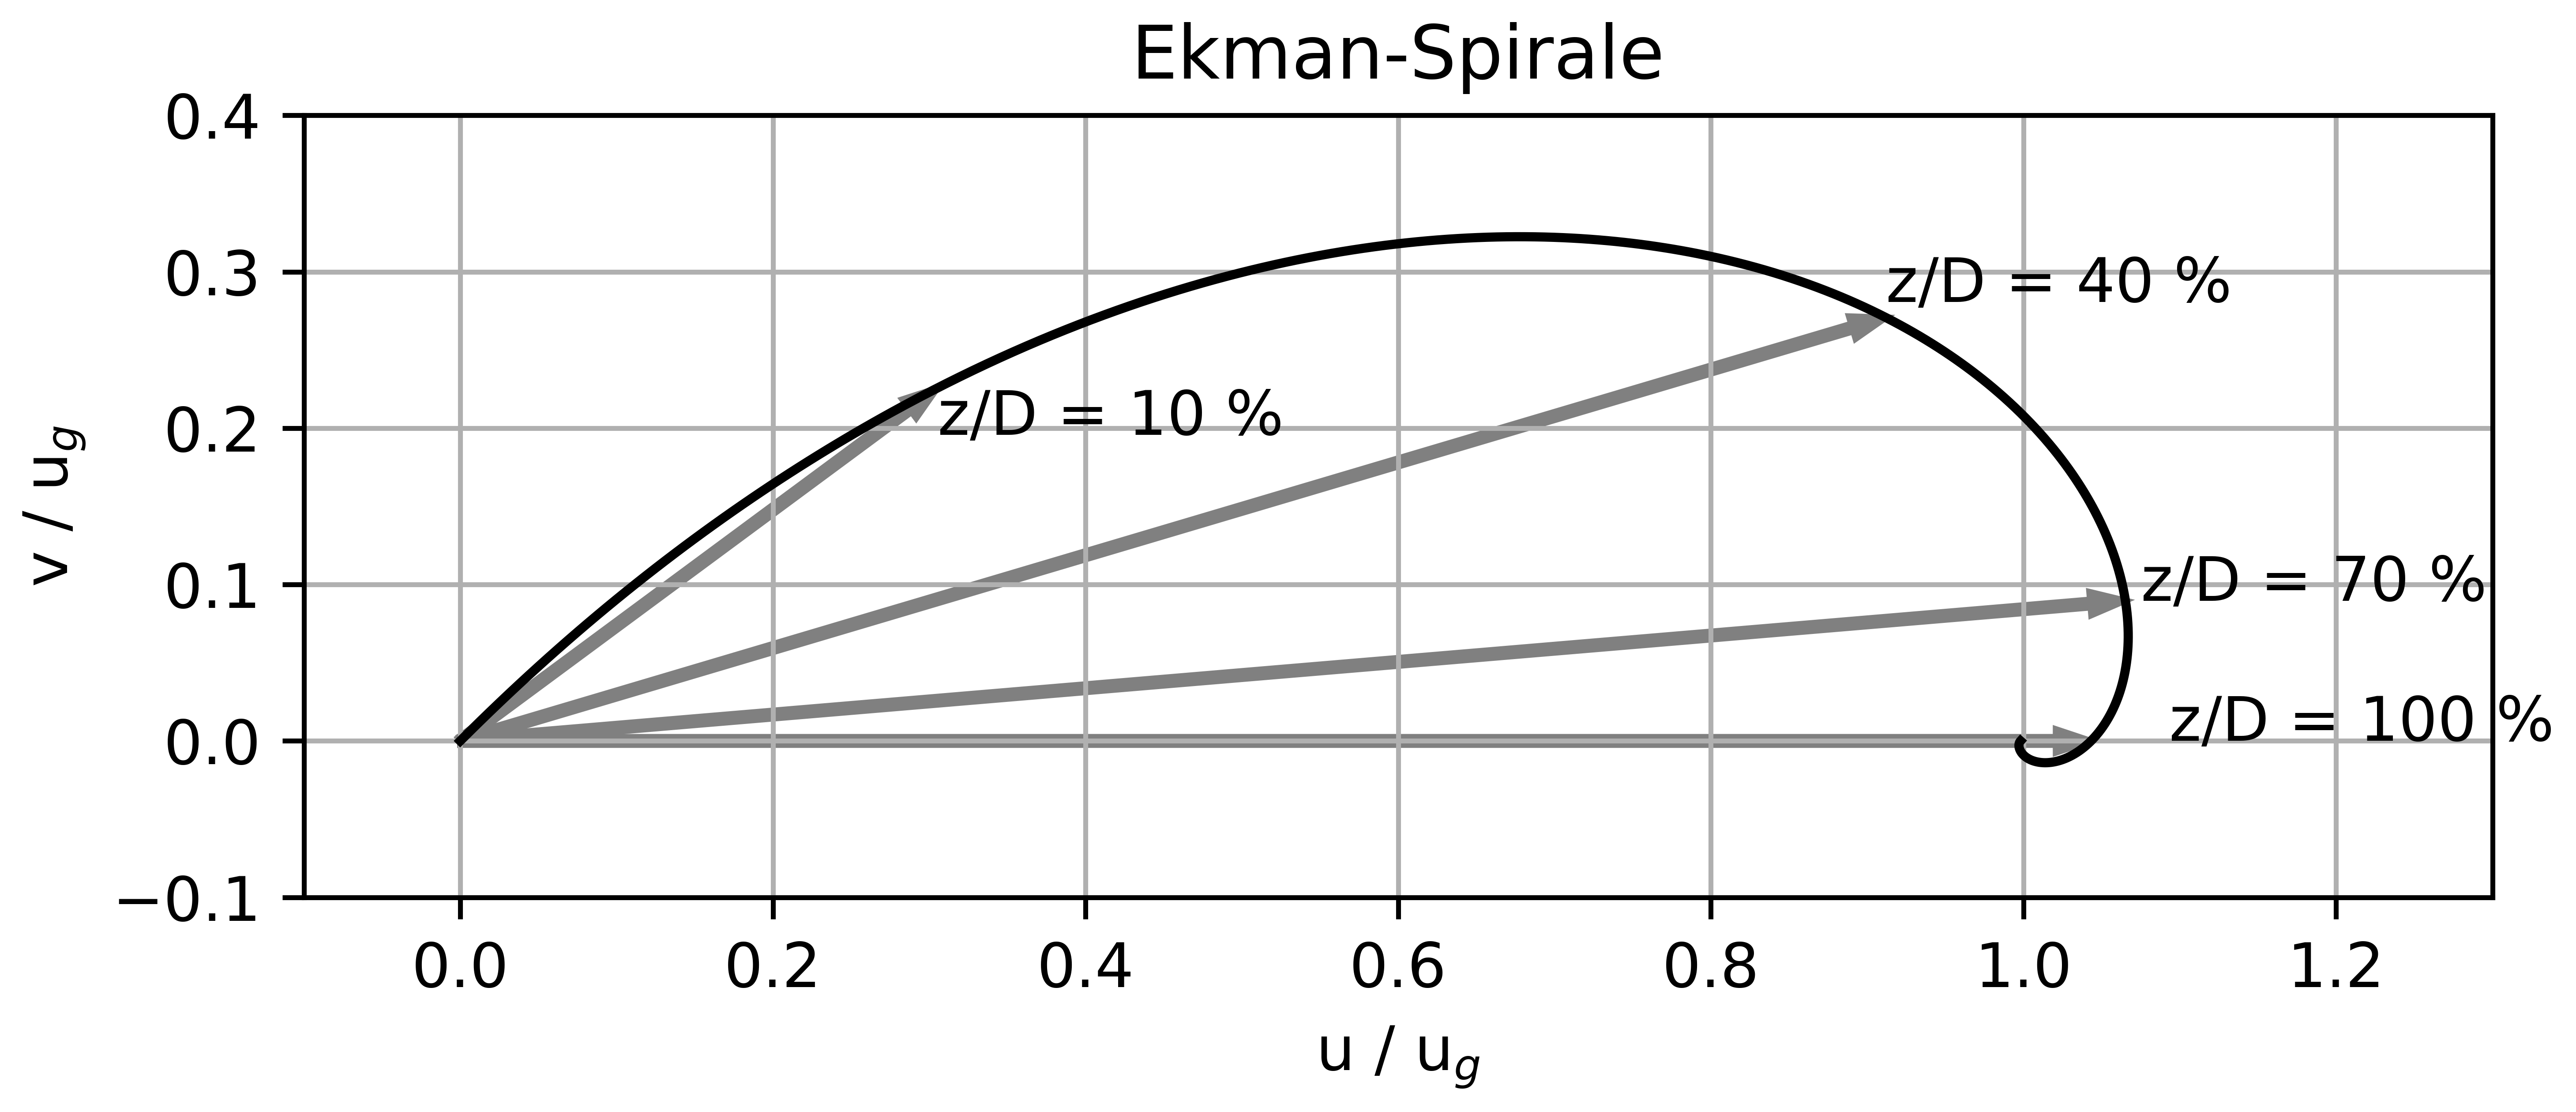
\includegraphics[width = 0.6\textwidth]{figs/ekman_spiral.png}
\caption{Die Ekman-Spirale, es ist $v_g = 0$.}
\label{fig:ekman_spiral}
\end{center}
\end{figure}
%
In einer isothermen Atmosphäre gilt
%
\begin{align}
\alpha = \sqrt{\frac{\left|f\right|}{2K}}, && \beta = -\sqrt{\frac{\left|f\right|}{2K}} - \frac{1}{H}\\
\Rightarrow \alpha^2 + \beta^2 = \frac{\left|f\right|}{K} + \frac{1}{H^2} + \sqrt{\frac{2\left|f\right|}{KH^2}} && \Rightarrow \frac{\alpha}{\beta^2 + \alpha^2} = \frac{1}{\sqrt{\frac{2\left|f\right|}{K}} + \sqrt{\frac{2K}{\left|f\right|H^4}} + \frac{2}{H}} = \frac{H}{2 + H\sqrt{\frac{2\left|f\right|}{K}} + \sqrt{\frac{2K}{fH^2}}}.
\end{align}
%
mit $H \approx 8$ km als Skalenhöhe. Die Höhe $D$, in der der Wind parallel zum geostrophischen Wind ist, verwendet man häufig als eine technische Definition der \textit{Dicke der Grenzschicht}\index{Dicke der Grenzschicht}\index{Grenzschicht!Dicke}. Es gilt
%
\begin{center}
\doublebox{\parbox{\textwidth}{
\begin{center}
\begin{align}
D & = \sqrt{\frac{2K}{\left|f\right|}}\pi
\end{align}
\end{center}
}}
\end{center}
%
Dort ist die Windgeschwindigkeit etwas höher als die geostrophische Geschwindigkeit, weshalb diese Höhe auch als \index{Gradientenwindhöhe}\textit{Gradientenwindhöhe} bezeichnet wird. Aus Beobachtungen weiß man, dass in ca. 1 km Höhe der Wind seinen geostrophischen Wert anstrebt, daraus folgt
%
\begin{align}
K \approx \frac{\left|f\right|D^2}{2\pi^2} \approx 5\text{ m}^2/\text{s}.
\end{align}
%
Dies ist über fünf Größenordnungen über dem Wert der kinematischen Viskosität von $1, 5\cdot 10^{-5}$ m$^2$/s. Mit Glg. \eqref{eq:def_eddy_exchange_coeff} folgt für die Mischungsweglänge
%
\begin{align}
l = \sqrt{\frac{K}{\left|\frac{\partial\newoverline{\mathbf{v}_h}}{\partial z}\right|}} \sim \sqrt{\frac{KD}{u_g}} \sim 2\cdot 10^1\text{ m}.
\end{align}
%
Dies entspricht der Erwartung, dass $l \ll D$ sein muss, damit das Mischungswegkonzept in der planetarischen Grenzschicht sinnvoll ist. Es ergibt sich mit Glg. \eqref{eq:karman_eq} eine Höhe $D_P$ der Prandtl-Schicht von ca.
%
\begin{align}
D_P = \frac{l}{k} = 50\text{ m}
\end{align}
%
mit $k = 0, 4$. Man definiert die \textit{Ekman-Zahl}\index{Ekman-Zahl} $\Ek$ als das Verhältnis von Reibungs- zu Coriolistermen, also
%
\begin{center}
\doublebox{\parbox{\textwidth}{
\begin{center}
\begin{align}
\Ek \coloneqq \frac{KU}{H^2fU} = \frac{K}{fH^2}, \label{eq:def_ekman_number}
\end{align}
\end{center}
}}
\end{center}
%
wobei $H$ die charakteristische Vertikalausdehnung des Phänomens ist. Bei kleinen Ekman-Zahlen kann die Reibungskraft durch die Coriolis-Kraft ausgeglichen werden. In der Grenzschicht erhält man eine Ekman-Zahl von $\Ek \sim 5$ \%.

Die Ekman-Spirale führt bei einer Zyklone mit Radius $R$ zu einer Drucktendenz $\frac{\partial p}{\partial t}$ in der Größenordnung
%
\begin{align}
\frac{\partial p}{\partial t} & \sim \frac{2g}{R}\frac{u_g\rho_0\alpha}{\beta^2 + \alpha^2}.
\end{align}
%
Man erhält mit $u_g \sim 10$ m/s, $\rho_0 \approx 1, 2$ kg/m$^3$ und $R \sim 500$ km
%
\begin{align}
\frac{\partial p}{\partial t} & \sim 2, 6\text{ }\frac{\text{hPa}}{\text{hr}}.
\end{align}
%
Dies ist deutlich geringer als der in Absch. \ref{sec:reibungswind} abgeschätzte Wert. Die Obergrenze der Grenzschicht ist gleichzeitig die Obergrenze der Ekman-Schicht.

\subsection{Spin-down}
\label{sec:spin-down}\index{Spin-down}

\section{Isotrope Turbulenz}
\label{sec:isotrope_turbulenz}\index{isotrope Turbulenz}\index{Turbulenz!isotrope}

\subsection{Spektralform der Navier-Stokes-Gleichungen}
\label{sec:spektralform_der_navier-stokes-gleichungen}\index{Navier-Stokes-Gleichungen!Spektralform}\index{Spektralform der Navier-Stokes-Gleichungen}

Für die Fourier-Transformation $\newtilde{\mathbf{v}}\left(\mathbf{k}, t\right)$ eines Geschwindigkeitsfeldes $\mathbf{v} = \mathbf{v}\left(\mathbf{r}, t\right)$ gilt
%
\begin{align}
\newtilde{\mathbf{v}}\left(\mathbf{k}, t\right) = C^3\int_{\mathbb{R}^3}\mathbf{v}\left(\mathbf{r}, t\right)\exp\left(-i\mathbf{k}\cdot\mathbf{r}\right)d^3r.
\end{align}
%
Die inverse Fourier-Transformation lautet
%
\begin{align}
\mathbf{v}\left(\mathbf{r}, t\right) = \newtilde{C}^3\int_{\mathbb{R}^3}\newtilde{\mathbf{v}}\left(\mathbf{k}, t\right)\exp\left(i\mathbf{k}\cdot\mathbf{r}\right)d^3k.\label{eq:velocity_field_ft_inv}
\end{align}
%
Man setzt an dieser Stelle $\newtilde{C} = 1 \stackrel{\text{Glg. \eqref{eq:ft_norm}}}{\Leftrightarrow} C = \frac{1}{2\pi}$ an, um die Notation abzukürzen und vernachlässigt das $\mathbb{R}^3$ am Integral. Die inkompressible Impulsgleichung lautet
%
\begin{align}
\frac{\partial\mathbf{v}}{\partial t} = -\nabla\pi - \nabla\varphi - \left(\mathbf{v}\cdot\nabla\right)\mathbf{v} + \nu\Delta\mathbf{v},
\end{align}
%
wobei die Abkürzung
%
\begin{align}
\pi\coloneqq\frac{p}{\rho}
\end{align}
%
eingesetzt wurde. Die inverse Fourier-Transformationen der anderen auftretenden Felder lauten
%
\begin{align}
\pi\left(\mathbf{r}, t\right) & = \int\newtilde{\pi}\left(\mathbf{k}, t\right)\exp\left(i\mathbf{k}\cdot\mathbf{r}\right)d^3k,\\
\varphi\left(\mathbf{r}\right) & = \int\newtilde{\varphi}\left(\mathbf{k}\right)\exp\left(i\mathbf{k}\cdot\mathbf{r}\right)d^3k.
\end{align}
%
Weiterhin gilt für die Anwendung der Differenzialoperatoren auf die Felder
%
\begin{align}
\frac{\partial\mathbf{v}}{\partial t} & = \int\frac{\partial\newtilde{\mathbf{v}}\left(\mathbf{k}, t\right)}{\partial t}\exp\left(i\mathbf{k}\cdot\mathbf{r}\right)d^3k,\\
-\nabla\pi & = -i\int\mathbf{k}\newtilde{\pi}\left(\mathbf{k}, t\right)\exp\left(i\mathbf{k}\cdot\mathbf{r}\right)d^3k,\\
-\nabla\varphi & = -i\int\mathbf{k}\newtilde{\varphi}\left(\mathbf{k}\right)\exp\left(i\mathbf{k}\cdot\mathbf{r}\right)d^3k,\\
\Delta\mathbf{v} & = -\int\mathbf{k}^2\newtilde{\mathbf{v}}\left(\mathbf{k}, t\right)\exp\left(i\mathbf{k}\cdot\mathbf{r}\right)d^3k.
\end{align}
%
Für die Impulsadvektion gilt
%
\begin{align}
\left(\mathbf{v}\cdot\nabla\right)\mathbf{v} & = \left(\int\newtilde{\mathbf{v}}\left(\mathbf{k}, t\right)\exp\left(i\mathbf{k}\cdot\mathbf{r}\right)d^3k\cdot\nabla\right)\int\newtilde{\mathbf{v}}\left(\mathbf{k}, t\right)\exp\left(i\mathbf{k}\cdot\mathbf{r}\right)d^3k\nonumber\\
& = \left(\int\newtilde{\mathbf{v}}\left(\mathbf{k}', t\right)\exp\left(i\mathbf{k}'\cdot\mathbf{r}\right)d^3k'\cdot\nabla\right)\int\newtilde{\mathbf{v}}\left(\mathbf{k}'', t\right)\exp\left(i\mathbf{k}''\cdot\mathbf{r}\right)d^3k''\nonumber\\
& = \int\int\exp\left(i\mathbf{k}'\cdot\mathbf{r}\right)\left[\newtilde{\mathbf{v}}\left(\mathbf{k}', t\right)\cdot\nabla\right]\left[\newtilde{\mathbf{v}}\left(\mathbf{k}'', t\right)\exp\left(i\mathbf{k}''\cdot\mathbf{r}\right)\right]d^3k'd^3k''\nonumber\\
& = i\int\int\left[\newtilde{\mathbf{v}}\left(\mathbf{k}', t\right)\cdot\mathbf{k}''\right]\newtilde{\mathbf{v}}\left(\mathbf{k}'', t\right)\exp\left[i\left(\mathbf{k}' + \mathbf{k}''\right)\cdot\mathbf{r}\right]d^3k'd^3k''.
\end{align}
%
Dies impliziert
%
\begin{align}
\left[\newtilde{\left(\mathbf{v}\cdot\nabla\right)\mathbf{v}}\right]\left(\mathbf{k}\right) & = \frac{i}{\left(2\pi\right)^3}\int\int\left[\newtilde{\mathbf{v}}\left(\mathbf{k}', t\right)\cdot\mathbf{k}''\right]\newtilde{\mathbf{v}}\left(\mathbf{k}'', t\right)\exp\left[i\left(-\mathbf{k} + \mathbf{k}' + \mathbf{k}''\right)\cdot\mathbf{r}\right]d^3k'd^3k''\nonumber\\
& \stackrel{\text{Glg. \eqref{eq:delta_distribution_prop_2}}}{=} i\int\int\left[\newtilde{\mathbf{v}}\left(\mathbf{k}', t\right)\cdot\mathbf{k}''\right]\newtilde{\mathbf{v}}\left(\mathbf{k}'', t\right)\delta\left(\mathbf{k}' + \mathbf{k}'' - \mathbf{k}\right)d^3k'd^3k''\nonumber\\
& = i\int\left[\newtilde{\mathbf{v}}\left(\mathbf{k}', t\right)\cdot\left(\mathbf{k} - \mathbf{k}'\right)\right]\newtilde{\mathbf{v}}\left(\mathbf{k} - \mathbf{k}', t\right)d^3k'
\end{align}
%
Aus der inkompressiblen Kontinuitätsgleichung
%
\begin{align}
\nabla\cdot\mathbf{v} = 0
\end{align}
%
folgt
%
\begin{center}
\doublebox{\parbox{\textwidth}{
\begin{center}
\begin{align}
\mathbf{k}\cdot\newtilde{\mathbf{v}}\left(\mathbf{k}, t\right) = 0.\label{eq:cont_incom_spec}
\end{align}
\end{center}
}}
\end{center}
%
Damit erhält man
%
\begin{align}
\left[\newtilde{\left(\mathbf{v}\cdot\nabla\right)\mathbf{v}}\right]\left(\mathbf{k}\right) & = i\int\left[\newtilde{\mathbf{v}}\left(\mathbf{k}', t\right)\cdot\mathbf{k}\right]\newtilde{\mathbf{v}}\left(\mathbf{k} - \mathbf{k}', t\right)d^3k'
\end{align}
%
Aus den bisherigen Rechnungen kann man die Entwicklung der Impulsgleichung bezüglich ebener Wellen\index{Impulsgleichung!Entwicklung nach ebenen Wellen} zusammensetzen:
%
\begin{align}
&  \int\left(\frac{\partial}{\partial t} + \nu\mathbf{k}^2\right)\newtilde{\mathbf{v}}\left(\mathbf{k}, t\right)\exp\left(i\mathbf{k}\cdot\mathbf{r}\right)d^3k\nonumber\\
& = i\int\left\{-\mathbf{k}\newtilde{\pi}\left(\mathbf{k}, t\right) - \mathbf{k}\newtilde{\varphi}\left(\mathbf{k}\right) - \int\left[\newtilde{\mathbf{v}}\left(\mathbf{k}', t\right)\cdot\mathbf{k}\right]\newtilde{\mathbf{v}}\left(\mathbf{k} - \mathbf{k}', t\right)d^3k'\right\}\exp\left(i\mathbf{k}\cdot\mathbf{r}\right)d^3k
\end{align}
%
Dies muss an jedem Punkt im Spektralraum gelten, also
%
\begin{center}
\doublebox{\parbox{\textwidth}{
\begin{center}
\begin{align}
\left(\frac{\partial}{\partial t} + \nu\mathbf{k}^2\right)\newtilde{\mathbf{v}}\left(\mathbf{k}, t\right) & = -i\mathbf{k}\newtilde{\pi}\left(\mathbf{k}, t\right) - i\mathbf{k}\newtilde{\varphi}\left(\mathbf{k}\right) - i\int\left[\newtilde{\mathbf{v}}\left(\mathbf{k}', t\right)\cdot\mathbf{k}\right]\newtilde{\mathbf{v}}\left(\mathbf{k} - \mathbf{k}', t\right)d^3k'.\label{eq:turbulence_inc_spec}
\end{align}
\end{center}
}}
\end{center}
%
Dies ist die Spektralform der inkompressiblen Impulsgleichung. Hieraus wird ersichtlich, dass der einzige Term, der Wechselwirkungen zwischen Skalen enthält, die Impulsadvektion ist.

\subsection{Energie-Transfer-Funktion}
\label{sec:energie-transfer-funktion}\index{Energie-Transfer-Funktion}

Wie man aus der Parseval-Identität\index{Parseval-Identität} Glg. \eqref{eq:parseval_identity} folgern kann, wird die spezifische kinetische Energie mit dem Wellenvektor $\mathbf{k}$ durch die Größe
%
\begin{align}
\newtilde{e}\left(\mathbf{k}, t\right) = \frac{1}{2}\newtilde{\mathbf{v}}\left(\mathbf{k}, t\right)\newtilde{\mathbf{v}}\left(-\mathbf{k}, t\right)
\end{align}
%
beschrieben. Notiert man Glg. \eqref{eq:turbulence_inc_spec} mit der Ersetzung $\mathbf{k} \to -\mathbf{k}$, erhält man
%
\begin{align}
\left(\frac{\partial}{\partial t} + \nu\mathbf{k}^2\right)\newtilde{\mathbf{v}}\left(-\mathbf{k}, t\right) & = i\mathbf{k}\newtilde{\pi}\left(-\mathbf{k}, t\right) + i\mathbf{k}\newtilde{\varphi}\left(-\mathbf{k}\right) + i\int\left[\newtilde{\mathbf{v}}\left(\mathbf{k}', t\right)\cdot\mathbf{k}\right]\newtilde{\mathbf{v}}\left(-\mathbf{k} - \mathbf{k}', t\right)d^3k'.\label{eq:deriv_turbulence_spec_0}
\end{align}
%
Multipliziert man Glg. \eqref{eq:deriv_turbulence_spec_0} mit $\newtilde{\mathbf{v}}\left(\mathbf{k}, t\right)$ und berücksichtigt dabei Glg. \eqref{eq:cont_incom_spec}, erhält man
%
\begin{align}
\newtilde{\mathbf{v}}\left(\mathbf{k}, t\right)\cdot\left(\frac{\partial}{\partial t} + \nu\mathbf{k}^2\right)\newtilde{\mathbf{v}}\left(-\mathbf{k}, t\right) & = i\int\left[\newtilde{\mathbf{v}}\left(\mathbf{k}', t\right)\cdot\mathbf{k}\right]\left[\newtilde{\mathbf{v}}\left(\mathbf{k}, t\right)\cdot\newtilde{\mathbf{v}}\left(-\mathbf{k} - \mathbf{k}', t\right)\right]d^3k'.\label{eq:deriv_turbulence_spec_1}
\end{align}
%
Multipliziert man analog Glg. \eqref{eq:turbulence_inc_spec} mit $\newtilde{\mathbf{v}}\left(-\mathbf{k}, t\right)$, erhält man
%
\begin{align}
\newtilde{\mathbf{v}}\left(-\mathbf{k}, t\right)\cdot\left(\frac{\partial}{\partial t} + \nu\mathbf{k}^2\right)\newtilde{\mathbf{v}}\left(\mathbf{k}, t\right) & = -i\int\left[\newtilde{\mathbf{v}}\left(\mathbf{k}', t\right)\cdot\mathbf{k}\right]\left[\newtilde{\mathbf{v}}\left(-\mathbf{k}, t\right)\cdot\newtilde{\mathbf{v}}\left(\mathbf{k} - \mathbf{k}', t\right)\right]d^3k'\label{eq:deriv_turbulence_spec_2}
\end{align}
%
Addiert man die Glg.en \eqref{eq:deriv_turbulence_spec_1} und \eqref{eq:deriv_turbulence_spec_2} und dividiert durch zwei, erhält man
%
\begin{align}
& \left(\frac{\partial}{\partial t} + 2\nu\mathbf{k}^2\right)\newtilde{e}\left(\mathbf{k}, t\right)\nonumber\\
& = \frac{i}{2}\int\left[\newtilde{\mathbf{v}}\left(\mathbf{k}', t\right)\cdot\mathbf{k}\right]\left[\newtilde{\mathbf{v}}\left(\mathbf{k}, t\right)\cdot\newtilde{\mathbf{v}}\left(-\mathbf{k} - \mathbf{k}', t\right)\right]d^3k' - \frac{i}{2}\int\left[\newtilde{\mathbf{v}}\left(\mathbf{k}', t\right)\cdot\mathbf{k}\right]\left[\newtilde{\mathbf{v}}\left(-\mathbf{k}, t\right)\cdot\newtilde{\mathbf{v}}\left(\mathbf{k} - \mathbf{k}', t\right)\right]d^3k'.
\end{align}
%
Substituiert man im ersten Integral mit $\mathbf{f}\left(\mathbf{k}'\right) = \mathbf{k}' - \mathbf{k}$ und im zweiten Integral mit $\mathbf{f}\left(\mathbf{k}'\right) = \mathbf{k} - \mathbf{k}'$, erhält man
%
\begin{align}
& \left(\frac{\partial}{\partial t} + 2\nu\mathbf{k}^2\right)\newtilde{e}\left(\mathbf{k}, t\right)\nonumber\\
& = \frac{i}{2}\int\left\{\left[\newtilde{\mathbf{v}}\left(\mathbf{k}' - \mathbf{k}, t\right)\cdot\mathbf{k}\right]\left[\newtilde{\mathbf{v}}\left(\mathbf{k}, t\right)\cdot\newtilde{\mathbf{v}}\left(-\mathbf{k}', t\right)\right] - \left[\newtilde{\mathbf{v}}\left(\mathbf{k} - \mathbf{k}', t\right)\cdot\mathbf{k}\right]\left[\newtilde{\mathbf{v}}\left(-\mathbf{k}, t\right)\cdot\newtilde{\mathbf{v}}\left(\mathbf{k}', t\right)\right]\right\}d^3k'.
\end{align}
%
Im zweiten Integral sei darauf hingewiesen, dass sich das Minuszeichen, welches aus dem Vertausch der Integrationsgrenzen folgt, mit demjenigen aufhebt, welches sich aus der Ableitung der substituierten Funktion ergibt. Man definiert die \textit{Energie-Transfer-Funktion}\index{Energie-Transfer-Funktion} $W = W\left(\mathbf{k}, \mathbf{k}', t\right)$ durch
%
\begin{align}
W\left(\mathbf{k}, \mathbf{k}', t\right) &\coloneqq \frac{i\mathbf{k}}{2}\cdot\left\{\newtilde{\mathbf{v}}\left(\mathbf{k}' - \mathbf{k}, t\right)\left[\newtilde{\mathbf{v}}\left(\mathbf{k}, t\right)\cdot\newtilde{\mathbf{v}}\left(-\mathbf{k}', t\right)\right] - \newtilde{\mathbf{v}}\left(\mathbf{k} - \mathbf{k}', t\right)\left[\newtilde{\mathbf{v}}\left(-\mathbf{k}, t\right)\cdot\newtilde{\mathbf{v}}\left(\mathbf{k}', t\right)\right]\right\}.\label{eq:def_energy_tranfer_function}
\end{align}
%
Damit erhält man die Bilanzgleichung der kinetischen Energie in spektraler Form\index{Bilanzgleichung!kinetische Energie}\index{kinetische Energie!Bilanzgleichung}\index{Energie!kinetische!Bilanzgleichung}
%
\begin{center}
\doublebox{\parbox{\textwidth}{
\begin{center}
\begin{align}
\left(\frac{\partial}{\partial t} + 2\nu\mathbf{k}^2\right)\newtilde{e}\left(\mathbf{k}, t\right) = \int W\left(\mathbf{k}, \mathbf{k}', t\right)d^3k'.\label{eq:e_kin_budget_spectral}
\end{align}
\end{center}
}}
\end{center}
%
Hieraus wird ersichtlich, dass die Reibung $\propto\frac{1}{L^2}$ skalensensitiv ist und in jedem Fall die spektrale spezifische kinetische Energie reduziert. Für die Energie-Transfer-Funktion\index{Energie-Transfer-Funktion} gilt
%
\begin{align}
W\left(\mathbf{k}', \mathbf{k}, t\right) & = \frac{i\mathbf{k}'}{2}\cdot\left\{\newtilde{\mathbf{v}}\left(\mathbf{k} - \mathbf{k}', t\right)\left[\newtilde{\mathbf{v}}\left(\mathbf{k}', t\right)\cdot\newtilde{\mathbf{v}}\left(-\mathbf{k}, t\right)\right] - \newtilde{\mathbf{v}}\left(\mathbf{k}' - \mathbf{k}, t\right)\left[\newtilde{\mathbf{v}}\left(-\mathbf{k}', t\right)\cdot\newtilde{\mathbf{v}}\left(\mathbf{k}, t\right)\right]\right\}\nonumber\\
& = -\frac{i\mathbf{k}'}{2}\cdot\left\{\newtilde{\mathbf{v}}\left(\mathbf{k}' - \mathbf{k}, t\right)\left[\newtilde{\mathbf{v}}\left(-\mathbf{k}', t\right)\cdot\newtilde{\mathbf{v}}\left(\mathbf{k}, t\right)\right] - \newtilde{\mathbf{v}}\left(\mathbf{k} - \mathbf{k}', t\right)\left[\newtilde{\mathbf{v}}\left(\mathbf{k}', t\right)\cdot\newtilde{\mathbf{v}}\left(-\mathbf{k}, t\right)\right]\right\}\nonumber\\
& = -\frac{i\mathbf{k}'}{2}\cdot\left\{\newtilde{\mathbf{v}}\left(\mathbf{k}' - \mathbf{k}, t\right)\left[\newtilde{\mathbf{v}}\left(\mathbf{k}, t\right)\cdot\newtilde{\mathbf{v}}\left(-\mathbf{k}', t\right)\right] - \newtilde{\mathbf{v}}\left(\mathbf{k} - \mathbf{k}', t\right)\left[\newtilde{\mathbf{v}}\left(-\mathbf{k}, t\right)\cdot\newtilde{\mathbf{v}}\left(\mathbf{k}', t\right)\right]\right\}
\end{align}
%
Hieraus folgt
%
\begin{align}
&  W\left(\mathbf{k}', \mathbf{k}, t\right) + W\left(\mathbf{k}, \mathbf{k}', t\right)\nonumber\\
& = \frac{i\mathbf{k}}{2}\cdot\left\{\newtilde{\mathbf{v}}\left(\mathbf{k}' - \mathbf{k}, t\right)\left[\newtilde{\mathbf{v}}\left(\mathbf{k}, t\right)\cdot\newtilde{\mathbf{v}}\left(-\mathbf{k}', t\right)\right] - \newtilde{\mathbf{v}}\left(\mathbf{k} - \mathbf{k}', t\right)\left[\newtilde{\mathbf{v}}\left(-\mathbf{k}, t\right)\cdot\newtilde{\mathbf{v}}\left(\mathbf{k}', t\right)\right]\right\}\nonumber\\
&  - \frac{i\mathbf{k}'}{2}\cdot\left\{\newtilde{\mathbf{v}}\left(\mathbf{k}' - \mathbf{k}, t\right)\left[\newtilde{\mathbf{v}}\left(\mathbf{k}, t\right)\cdot\newtilde{\mathbf{v}}\left(-\mathbf{k}', t\right)\right] - \newtilde{\mathbf{v}}\left(\mathbf{k} - \mathbf{k}', t\right)\left[\newtilde{\mathbf{v}}\left(-\mathbf{k}, t\right)\cdot\newtilde{\mathbf{v}}\left(\mathbf{k}', t\right)\right]\right\}\nonumber\\
& = \frac{i}{2}\left[\newtilde{\mathbf{v}}\left(\mathbf{k}, t\right)\cdot\newtilde{\mathbf{v}}\left(-\mathbf{k}', t\right)\right]\newtilde{\mathbf{v}}\left(\mathbf{k}' - \mathbf{k}, t\right)\cdot\left(\mathbf{k} - \mathbf{k}'\right)\nonumber\\
&  -\frac{i}{2}\left[\newtilde{\mathbf{v}}\left(-\mathbf{k}, t\right)\cdot\newtilde{\mathbf{v}}\left(\mathbf{k}', t\right)\right]\newtilde{\mathbf{v}}\left(\mathbf{k} - \mathbf{k}', t\right)\cdot\left(\mathbf{k} - \mathbf{k}'\right)\nonumber\\
& \stackrel{\text{Glg. \eqref{eq:cont_incom_spec}}}{=} 0.
\end{align}
%
Die Energie-Transfer-Funktion ist also antisymmetrisch\index{Energie-Transfer-Funktion!Antisymmetrie}\index{Antisymmetrie der Energie-Transfer-Funktion}:
%
\begin{center}
\doublebox{\parbox{\textwidth}{
\begin{center}
\begin{align}
W\left(k, k', t\right) = -W\left(k, k', t\right)\label{eq:energy_tranfer_function_antisymmetric}
\end{align}
\end{center}
}}
\end{center}
%
Dies hängt mit der Energieerhaltung zusammen: Der Energiegewinn der Komponente $\mathbf{k}$ auf Kosten der Komponente $\mathbf{k}'$ ist gleich dem Energieverlust der Komponente $\mathbf{k}'$ aufgrund der Komponente $\mathbf{k}$.

\subsubsection{Isotrope Form}
\label{sec:isotrope_form}\index{isotrope Form der Energie-Transfer-Funktion}\index{Energie-Transfer-Funktion!isotrope Form}

Nun macht man die Annahme der Isotropie\index{Isotropie}, d. h. man geht geht davon aus, dass spektrale Eigenschaften nicht von den drei Komponente des Vektors $\mathbf{k}$ abhängen, sondern ausschließlich vom Betrag von $k$, also
%
\begin{align}
e\left(\mathbf{k}, t\right) \to \frac{\newtilde{e}\left(k, t\right)}{4\pi k^2}, && W\left(\mathbf{k}, \mathbf{k}, t\right) \to \frac{W\left(k, k', t\right)}{4\pi k'^24\pi k^2}.
\end{align}
%
Dabei wurde für die Geometrie der Kugelkoordinaten korrigiert. Somit wird Glg. \eqref{eq:e_kin_budget_spectral} zu
%
\begin{align}
\left(\frac{\partial}{\partial t} + 2\nu k^2\right)\frac{\newtilde{e}\left(k, t\right)}{4\pi k^2} & = \int\frac{W\left(k, k', t\right)}{4\pi k'^24\pi k^2}4\pi k'^2dk'\nonumber
\end{align}
\begin{center}
\doublebox{\parbox{\textwidth}{
\begin{center}
\begin{align}
\Rightarrow\left(\frac{\partial}{\partial t} + 2\nu k^2\right)\newtilde{e}\left(k, t\right) & = \int W\left(k, k', t\right)dk'.
\end{align}
\end{center}
}}
\end{center}

\subsection{Heisenberg-Ansatz}
\label{sec:heisenberg-ansatz}\index{Heisenberg-Ansatz}

Beim \textit{Heisenberg-Ansatz}\index{Heisenberg-Ansatz} wird zunächst von Stationarität ausgegangen, also
%
\begin{align}
2\nu k^2\newtilde{e}\left(k\right) & = \int W\left(k, k'\right)dk'.\label{eq:heisenberg_turb_0}
\end{align}
%
Weiterhin nimmt man an, dass es eine Grenz-Wellenzahl $k^\star$ gibt, welche das Spektrum in zwei Regionen aufteilt:
%
\begin{itemize}
\item Die Region $k < k^\star$ (größere Wellenlängen) bezeichnet man als Region 1. Hier kann aus geometrischen Gründen keine Isotropie angenommen werden. Der Heisenberg-Ansatz\index{Heisenberg-Ansatz} macht über diesen Bereich keine Aussagen.
\item Die Region $k \geq k^\star$ (kleinere Wellenlängen) bezeichnet man als \textit{universality region}\index{universality region}. Hier kann von Isotropie ausgegangen werden und die Strömung wird wenig von Randbedingungen beeinflusst.
\end{itemize}
%
Der Heisenberg-Ansatz\index{Heisenberg-Ansatz} bezieht sich ausschließlich auf die universality region\index{universality region}. Es wird dabei angenommen, dass die kleineren Skalen auf die größeren Skalen eine ähnliche Wirkung haben wie die Viskosität\index{Viskosität} auf die kleinstskaligen Wirbel: sie diffundieren Impuls. Dies ist gerechtfertigt, da davon ausgegangen werden kann, dass die kleinerskaligen Wirbel im Mittel Impuls diffundieren (Gradienten des Geschwindigkeitsfeldes abbauen). Der Heisenberg-Ansatz\index{Heisenberg-Ansatz} lautet als Formel
%
\begin{align}
W\left(k, k'\right) = -2\kappa_Hk^2\newtilde{e}\left(k\right)g\left(k', \newtilde{e}\left(k'\right)\right),
\end{align}
%
wobei von $k, k' \geq k^\star$ und $k' > k$ ausgegangen wird. $\kappa_H \geq 0$ ist eine Art dimensionslose Viskosität\index{Viskosität}, die sogenannte \textit{Heisenberg-Konstante}\index{Heisenberg-Konstante}. Diese Formel ist analog zum molekularen dissipativen Term $-2\nu k^2\newtilde{e}\left(k\right)$. Die Funktion $g\left(k', \newtilde{e}\left(k'\right)\right)$ beschreibt, wie die kleinere Skala $k'$ auf die auf die Skala $k$ wirkt, wobei eine explizite Abhängigkeit von der bei $k'$ vorhandenen Energie $\newtilde{e}\left(k'\right)$ mit aufgenommen wurde. Im SI-Sytem gelten
%
\begin{align}
\left[\newtilde{e}\right] & = \frac{\text{J}}{\text{kg/m}} = \frac{\text{Jm}}{\text{kg}} = \frac{\text{Nm}^2}{\text{kg}} = \frac{\text{m}^3}{\text{s}^2}\\
\Rightarrow \left[\frac{\partial\newtilde{e}}{\partial t}\right] = \frac{\text{m}^3}{\text{s}^3}, && \left[W\right] = \frac{\text{m}^4}{\text{s}^3}, && \Rightarrow \left[k^2\newtilde{e}\left(k\right)\right] = \frac{\text{m}}{\text{s}^2} && \Rightarrow \left[g\left(k', \newtilde{e}\left(k'\right)\right)\right] = \frac{\text{m}^3}{\text{s}}.
\end{align}
%
Als Ansatz für $g$ wählt man nun
%
\begin{align}
g\left(k', \newtilde{e}\left(k'\right)\right) = \left(k'\right)^\alpha\newtilde{e}\left(k'\right)^\beta.
\end{align}
%
Dies impliziert
%
\begin{align}
\beta & = \frac{1}{2}, \alpha = -\frac{3}{2}\\
\Rightarrow g\left(k', \newtilde{e}\left(k'\right)\right) & = \left(k'\right)^{-3/2}\newtilde{e}\left(k'\right)^{1/2} = \sqrt{\frac{\newtilde{e}\left(k'\right)}{\left(k'\right)^3}}.
\end{align}
%
Zusammenfassend lautet der Heisenberg-Ansatz\index{Heisenberg-Ansatz} also
%
\begin{align}
T\left(k, k'\right) = \begin{cases}
-2\kappa_Hk^2\newtilde{e}\left(k\right)\newtilde{e}\left(k'\right)^{1/2}\left(k'\right)^{-3/2},\text{ falls }k' \geq k\text{ gilt (Energieverlust an kleinere Skala),}\\
2\kappa_Hk^2\newtilde{e}\left(k\right)\newtilde{e}\left(k'\right)^{1/2}\left(k'\right)^{-3/2},\text{ falls }k' < k\text{ gilt (Energiegewinn von größerer Skala).}
\end{cases}\label{eq:heisenberg-ansatz}
\end{align}
%
Im Rahmen der Stationarität wird die durch Dissipation\index{Dissipation} verlorene kinetische Energie durch die Zufuhr von den größeren Skalen kompensiert. Die größeren Skalen haben also einen Energieverlust an die kleineren Skalen, welcher durch eine Produktion $\sigma\left(k\right)$ von kinetischer Energie kompensiert werden muss. Der Mechanismus, über welchen dies passiert, wird hier offengelassen. Man geht jedoch von $\sigma\left(k\right) = 0$ für $k > k^\star$ aus, um die Betrachtungen in der universality region\index{universality region} zu vereinfachen. Glg. \eqref{eq:heisenberg_turb_0} wird damit zu
%
\begin{align}
2\nu k^2\newtilde{e}\left(k\right) & = \int W\left(k, k'\right)dk' + \sigma\left(k\right).\label{eq:heisenberg_turb_1}
\end{align}

\subsection{Integrationen}
\label{sec:integrationen}

Integriert man Glg. \eqref{eq:heisenberg_turb_1} bis zu einer Wellenzahl $k > k^\star$, erhält man
%
\begin{align}
2\nu\int_0^k\left(k'\right)^2\newtilde{e}\left(k'\right)dk' & = \int_0^k\int_0^\infty W\left(k', k''\right)dk''dk' + \int_0^k\sigma\left(k'\right)dk'.\label{eq:heisenberg_turb_2}
\end{align}
%
Für $k = \infty$ erhält man
%
\begin{align}
2\nu\int_0^\infty\left(k'\right)^2\newtilde{e}\left(k'\right)dk' & = \int_0^\infty\int_0^\infty W\left(k', k''\right)dk''dk' + \int_0^\infty\sigma\left(k'\right)dk'.
\end{align}
%
Aufgrund der Antisymmetrie der Energie-Transfer-Funktion\index{Energie-Transfer-Funktion} $W\left(k', k''\right) = -W\left(k'', k'\right)$ gilt
%
\begin{align}
\int_0^\infty\int_0^\infty W\left(k', k''\right)dk''dk' = 0.
\end{align}
%
Dies entspricht der Tatsache, dass die Energie-Transfer-Funktion\index{Energie-Transfer-Funktion} kinetische Energie umverteilt, aber keine kinetische Energie produziert oder vernichtet. Dies führt auf
%
\begin{align}
2\nu\int_0^\infty\left(k'\right)^2\newtilde{e}\left(k'\right)dk' = \int_0^\infty\sigma\left(k'\right)dk'.
\end{align}
%
Dies entspricht der Tatsache, dass unter stationären Bedingungen ist die Energiezufuhr gleich dem Energieverlust ist. Der Energieverlust ist gleich der Dissipation\index{Dissipation}:
%
\begin{align}
\epsilon = 2\nu\int_0^\infty\left(k'\right)^2\newtilde{e}\left(k'\right)dk'
\end{align}
%
Wegen $k > k^\star$ und $\sigma\left(k'\right) = 0$ für $k' > k^\star$ gilt
%
\begin{align}
\int_0^k\sigma\left(k'\right)dk' = \int_0^\infty\sigma\left(k'\right)dk'.
\end{align}
%
Somit kann man Glg. \eqref{eq:heisenberg_turb_2} in der Form
%
\begin{align}
2\nu\int_0^k\left(k'\right)^2\newtilde{e}\left(k'\right)dk' & = \int_0^k\int_0^\infty W\left(k', k''\right)dk''dk' + \epsilon
\end{align}
%
aufschreiben. Wiederum wegen der Antisymmetrie $W\left(k', k''\right) = -W\left(k'', k'\right)$ gilt
%
\begin{align}
\int_0^k\int_0^kW\left(k', k''\right)dk''dk' = 0.
\end{align}
%
Somit gilt
%
\begin{align}
2\nu\int_0^k\left(k'\right)^2\newtilde{e}\left(k'\right)dk' & = \int_0^k\int_k^\infty W\left(k', k''\right)dk''dk' + \epsilon\nonumber\\
\Leftrightarrow \epsilon & = 2\nu\int_0^k\left(k'\right)^2\newtilde{e}\left(k'\right)dk' - \int_0^k\int_k^\infty W\left(k', k''\right)dk''dk''.
\end{align}
%
Setzt man hier Glg. \eqref{eq:heisenberg-ansatz} ein und beachtet $k'' > k'$, erhält man
%
\begin{align}
\epsilon & = 2\nu\int_0^k\left(k'\right)^2\newtilde{e}\left(k'\right)dk' - \int_0^k\int_k^\infty-2\kappa_H\left(k'\right)^2\newtilde{e}\left(k'\right)\newtilde{e}\left(k''\right)^{1/2}\left(k''\right)^{-3/2}dk''dk'\nonumber\\
\Leftrightarrow \epsilon & = 2\nu\int_0^k\left(k'\right)^2\newtilde{e}\left(k'\right)dk' + 2\kappa_H\int_0^k\int_k^\infty\left(k'\right)^2\newtilde{e}\left(k'\right)\newtilde{e}\left(k''\right)^{1/2}\left(k''\right)^{-3/2}dk''dk'\nonumber\\
\Leftrightarrow \epsilon & = 2\nu\int_0^k\left(k'\right)^2\newtilde{e}\left(k'\right)dk' + 2\kappa_H\int_k^\infty\newtilde{e}\left(k''\right)^{1/2}\left(k''\right)^{-3/2}dk''\int_0^k\left(k'\right)^2\newtilde{e}\left(k'\right)dk'\nonumber\\
\Leftrightarrow \epsilon & = 2\nu\int_0^k\left(k'\right)^2\newtilde{e}\left(k'\right)dk' + 2\kappa_H\int_k^\infty\sqrt{\frac{\newtilde{e}\left(k''\right)}{\left(k''\right)^3}}dk''\int_0^k\left(k'\right)^2\newtilde{e}\left(k'\right)dk'\nonumber\\
\Leftrightarrow\epsilon & = \left(2\nu + 2\kappa_H\int_k^\infty\sqrt{\frac{\newtilde{e}\left(k''\right)}{\left(k''\right)^3}}dk''\right)\int_0^k\left(k'\right)^2\newtilde{e}\left(k'\right)dk'.\label{eq:heisenberg_turb_3}
\end{align}
%
Die Größe
%
\begin{align}
K \coloneqq \kappa_H\int_k^\infty\sqrt{\frac{\newtilde{e}\left(k'\right)}{\left(k'\right)^3}}dk'
\end{align}
%
hat die Dimension ener Viskosität\index{Viskosität} und wird als \textit{Heisenberg'scher Austauschkoeffizient}\index{Heisenberg'scher Austauschkoeffizient} bezeichnet.

Man definiert nun eine Hilfsfunktion
%
\begin{align}
f\left(k\right) \coloneqq 2\int_0^k\left(k'\right)^2\newtilde{e}\left(k'\right)dk' \Rightarrow f'\left(k\right) = 2k^2\newtilde{e}\left(k\right).\label{eq:heisenberg_turb_6}
\end{align}
%
Hiermit kann man Glg. \eqref{eq:heisenberg_turb_3} in der Form
%
\begin{align}
\frac{\epsilon}{f\left(k\right)} = \nu + \kappa_H\int_k^\infty\sqrt{\frac{\newtilde{e}\left(k'\right)}{\left(k'\right)^3}}dk' = \nu + \kappa_H\int_k^\infty\sqrt{\frac{f'\left(k'\right)}{2\left(k'\right)^5}}dk'\label{eq:heisenberg_turb_5}
\end{align}
%
notieren. Differenziert man diese Gleichung, erhält man
%
\begin{align}
-\frac{\epsilon f'\left(k\right)}{f\left(k\right)^2} = -\kappa_H\sqrt{\frac{f'\left(k\right)}{2k^5}} \Rightarrow \frac{\epsilon^2f'\left(k\right)^2}{f\left(k\right)^4} = \kappa_H^2\frac{f'\left(k\right)}{2k^5} \Leftrightarrow \frac{\epsilon^2f'\left(k\right)}{f\left(k\right)^4} = \frac{\kappa_H^2}{2k^5}.
\end{align}
%
Integriert man beide Seiten über $k$, erhält man
%
\begin{align}
-\frac{\epsilon^2}{3f\left(k\right)^3} + C = -\frac{\kappa_H^2}{8k^4} \Leftrightarrow \frac{\epsilon^2}{3f\left(k\right)^3} = C + \frac{\kappa_H^2}{8k^4}\label{eq:heisenberg_turb_4}
\end{align}
%
mit einer Integrationskonstante $C$. Um diese zu bestimmen, betrachtet man Glg. \eqref{eq:heisenberg_turb_4} für $k \to \infty$:
%
\begin{align}
C = \frac{\epsilon^2}{3f\left(\infty\right)^3}
\end{align}
%
Um $f\left(\infty\right)$ zu bestimmen, wertet man Glg. \eqref{eq:heisenberg_turb_5} für $k \to \infty$ aus:
%
\begin{align}
\frac{\epsilon}{f\left(\infty\right)} & = \nu \Rightarrow f\left(\infty\right) = \frac{\epsilon}{\nu}\nonumber\\
\Rightarrow C & = \frac{\epsilon^2}{3f\left(\infty\right)^3} = \frac{\nu^3}{3\epsilon}
\end{align}
%
Setzt man dies in Glg. \eqref{eq:heisenberg_turb_4} ein, erhält man
%
\begin{align}
\frac{\epsilon^2}{3f\left(k\right)^3} & = \frac{\nu^3}{3\epsilon} + \frac{\kappa_H^2}{8k^4}\nonumber\\
\Rightarrow f\left(k\right)^3 & = \frac{\epsilon^2}{3}\left(\frac{\kappa_H^2}{8k^4} + \frac{\nu^3}{3\epsilon}\right)^{-1}\nonumber\\
\Rightarrow f\left(k\right) & = \frac{\epsilon^{2/3}}{3^{1/3}}\left(\frac{\kappa_H^2}{8k^4} + \frac{\nu^3}{3\epsilon}\right)^{-1/3}.
\end{align}
%
Differenziert man dies nach $k$, erhält man
%
\begin{align}
f'\left(k\right) & = \frac{\epsilon^{2/3}}{3^{1/3}}\frac{4}{3}\frac{\kappa_H^2}{8k^5}\left(\frac{\kappa_H^2}{8k^4} + \frac{\nu^3}{3\epsilon}\right)^{-4/3}.
\end{align}
%
Setzt man hier Glg. \eqref{eq:heisenberg_turb_6} ein, erhält man
%
\begin{align}
2k^2\newtilde{e}\left(k\right) & = \frac{\epsilon^{2/3}}{3^{1/3}}\frac{4}{3}\frac{\kappa_H^2}{8k^5}\left(\frac{\kappa_H^2}{8k^4} + \frac{\nu^3}{3\epsilon}\right)^{-4/3}\nonumber\\
\Leftrightarrow \newtilde{e}\left(k\right) & = \frac{\epsilon^{2/3}}{3^{1/3}}\frac{2}{3}\frac{\kappa_H^2}{8k^7}\left(\frac{\kappa_H^2}{8k^4} + \frac{\nu^3}{3\epsilon}\right)^{-4/3}\nonumber\\
\Leftrightarrow \newtilde{e}\left(k\right) & = \frac{\epsilon^{2/3}}{3^{1/3}}\frac{2}{3k^3}\frac{\kappa_H^2}{8k^4}\left(\frac{\kappa_H^2}{8k^4} + \frac{\nu^3}{3\epsilon}\right)^{-4/3}\nonumber\\
\Leftrightarrow \newtilde{e}\left(k\right) & = \frac{\epsilon^{2/3}}{3^{1/3}}\frac{2}{3k^3}\left(\frac{\kappa_H^2}{8k^4}\right)^{-1/3}\left(\frac{\kappa_H^2}{8k^4}\right)^{4/3}\left(\frac{\kappa_H^2}{8k^4} + \frac{\nu^3}{3\epsilon}\right)^{-4/3}\nonumber
\end{align}
\begin{align}
\Leftrightarrow \newtilde{e}\left(k\right) & = \frac{\epsilon^{2/3}}{3^{1/3}}\frac{2}{3k^3}\left(\frac{\kappa_H^2}{8k^4}\right)^{-1/3}\left(\frac{8k^4}{\kappa_H^2}\right)^{-4/3}\left(\frac{\kappa_H^2}{8k^4} + \frac{\nu^3}{3\epsilon}\right)^{-4/3}\nonumber\\
\Leftrightarrow \newtilde{e}\left(k\right) & = \frac{\epsilon^{2/3}}{3^{1/3}}\frac{2}{3k^3}\left(\frac{\kappa_H^2}{8k^4}\right)^{-1/3}\left(1 + \frac{8\nu^3k^4}{3\epsilon\kappa_H^2}\right)^{-4/3}\nonumber\\
\Leftrightarrow \newtilde{e}\left(k\right) & = \frac{\epsilon^{2/3}}{3^{1/3}}\frac{2}{3}\left(\frac{\kappa_H^2}{8}\right)^{-1/3}k^{-5/3}\left(1 + \frac{8\nu^3k^4}{3\epsilon\kappa_H^2}\right)^{-4/3}\nonumber\\
\Leftrightarrow \newtilde{e}\left(k\right) & = \left(\frac{8^2}{3^4\kappa_H^2}\right)^{1/3}\epsilon^{2/3}k^{-5/3}\left(1 + \frac{8\nu^3k^4}{3\epsilon\kappa_H^2}\right)^{-4/3}\nonumber\\
\Leftrightarrow \newtilde{e}\left(k\right) & = \left(\frac{8}{9\kappa_H}\right)^{2/3}\epsilon^{2/3}k^{-5/3}\left(1 + \frac{8\nu^3k^4}{3\epsilon\kappa_H^2}\right)^{-4/3}.\label{eq:turb_iso_inc_spec_pre_0}
\end{align}

\subsection{Ergebnisse}
\label{sec:ergebnisse}

Der Ausgangspunkt dieses Abschnittes ist Glg. \eqref{eq:turb_iso_inc_spec_pre_0}. Man definiert zunächst einige Abkürzungen. Zunächst definiert man
%
\begin{align}
k_c \coloneqq \left(\frac{\epsilon}{\nu^3}\right)^{1/4}.
\end{align}
%
Damit wird Glg. \eqref{eq:turb_iso_inc_spec_pre_1} zu
%
\begin{align}
\newtilde{e}\left(k\right) & = \left(\frac{8}{9\kappa_H}\right)^{2/3}\epsilon^{2/3}k^{-5/3}\left(1 + \frac{8k^4}{3\kappa_H^2k_c^4}\right)^{-4/3}.\label{eq:turb_iso_inc_spec_pre_1}
\end{align}
%
Weiterhin definiert man die \textit{Kolmogorov-Konstante}\index{Kolmogorov-Konstante} $\kappa_K$ durch
%
\begin{align}
\kappa_K \coloneqq \left(\frac{8}{9\kappa_H}\right)^{2/3},
\end{align}
%
die \textit{charakteristische Länge}\index{charakteristische Länge}\index{Länge!charakteristische} $l_c$ durch
%
\begin{align}
l_c \coloneqq \left(\frac{\nu^3}{\epsilon}\right)^{1/4}
\end{align}
%
sowie die \textit{charakteristische Zeit}\index{charakteristische Zeit}\index{Zeit!charakteristische} $t_c$ durch
%
\begin{align}
t_c \coloneqq \left(\frac{\nu}{\epsilon}\right)^{1/2}.
\end{align}
%
Hieraus folgt
%
\begin{align}
k_c = \frac{1}{l_c}.
\end{align}
%
Setzt man dies in Glg. \eqref{eq:turb_iso_inc_spec_pre_1} ein, erhält man 
%
\begin{center}
\doublebox{\parbox{\textwidth}{
\begin{center}
\begin{align}
\newtilde{e}\left(k\right) & = \kappa_K\epsilon^{2/3}k^{-5/3}\left(1 + \frac{8k^4l_c^4}{3\kappa_H^2}\right)^{-4/3} = \kappa_K\epsilon^{2/3}k^{-5/3}\left(1 + \frac{8k^4}{3\kappa_H^2k_c^4}\right)^{-4/3}.\label{eq:turb_iso_inc_spec}
\end{align}
\end{center}
}}
\end{center}
%
Hieraus lassen sich noch zwei wichtige Grenzfälle ableiten. Für $k > \sqrt{\kappa_H}k_c$ gilt
%
\begin{align}
\newtilde{e}\left(k\right) & \approx \left(\frac{8}{9\kappa_H}\right)^{2/3}\epsilon^{2/3}k^{-5/3}\left(\frac{8k^4l_c^4}{3\kappa_H^2}\right)^{-4/3} = \left(\frac{8\epsilon}{9\kappa_H}\right)^{2/3}\left(\frac{8\nu^3}{3\epsilon\kappa_H^2}\right)^{-4/3}k^{-7}\nonumber\\
& = \left(\frac{8\epsilon}{9\kappa_H}\right)^{2/3}\left(\frac{3\epsilon\kappa_H^2}{8\nu^3}\right)^{4/3}k^{-7}\nonumber
\end{align}
\begin{center}
\doublebox{\parbox{\textwidth}{
\begin{center}
\begin{align}
\Leftrightarrow\newtilde{e}\left(k\right) & \approx \left(\frac{\kappa_H\epsilon}{2\nu^2}\right)^{2}k^{-7}.
\end{align}
\end{center}
}}
\end{center}
%
Dieses Gebiet des Spektrums ($k > k_c$) bezeichnet man als \textit{dissipative range}\index{dissipative range}. In diesem Bereich führt die Viskosität\index{Viskosität} zu einem steilen Abfall des Spektrums. Im Fall $k^\star < k \ll k_c$ gilt
%
\begin{center}
\doublebox{\parbox{\textwidth}{
\begin{center}
\begin{align}
\newtilde{e}\left(k\right) & \approx \kappa_K\epsilon^{2/3}k^{-5/3}.
\end{align}
\end{center}
}}
\end{center}
%
Diesen Bereich des Spektrums ($k^\star < k \ll k_c$) bezeichnet man als \textit{inertial subrange}\index{inertial subrange}.

\section{Geostrophische Turbulenz}
\label{sec:geostrophische_turbulenz}\index{geostrophische Turbulenz}\index{Turbulenz!geostrophische}

Wendet man den Operator $\nabla\times$ auf Glg. \eqref{eq:velocity_field_ft_inv} in zwei Dimensionen an, erhält man
%
\begin{align}
\zeta &= \mathbf{e}_z\cdot\nabla\times\mathbf{v} = \mathbf{e}_z\cdot\nabla\times\int_{\mathbb{R}^2}\newtilde{\mathbf{v}}\left(\mathbf{k}\right)\exp\left(i\mathbf{k}\cdot\mathbf{r}\right)d^2r = \mathbf{e}_z\cdot\int_{\mathbb{R}^2}\nabla\times\left[\newtilde{\mathbf{v}}\left(\mathbf{k}\right)\exp\left(i\mathbf{k}\cdot\mathbf{r}\right)\right]d^2r\nonumber\\
&\stackrel{\text{Glg. \eqref{eq:diff_op_harmonic_rule_1}}}{=} \mathbf{e}_z\cdot\int_{\mathbb{R}^2}i\newtilde{\mathbf{v}}\left(\mathbf{k}\right)\exp\left(i\mathbf{k}\cdot\mathbf{r}\right)\times\mathbf{k}d^2r = \int_{\mathbb{R}^2}\mathbf{e}_z\cdot\left[i\newtilde{\mathbf{v}}\left(\mathbf{k}\right)\times\mathbf{k}\right]\exp\left(i\mathbf{k}\cdot\mathbf{r}\right)d^2r.
\end{align}
%
Hieraus folgt
%
\begin{align}
\newtilde{\zeta}\left(\mathbf{k}\right) = \mathbf{e}_z\cdot\left[i\newtilde{\mathbf{v}}\left(\mathbf{k}\right)\times\mathbf{k}\right].
\end{align}
%
Aus der Parseval-Identität Glg. \eqref{eq:parseval_identity} erhält man
%
\begin{align}
\newtilde{\zeta^2}\left(\mathbf{k}\right) &= -4\pi^2i\left(\newtilde{\mathbf{v}}\left(-\mathbf{k}\right)\times\mathbf{k}\right)\cdot i\left(\newtilde{\mathbf{v}}\left(\mathbf{k}\right)\times\mathbf{k}\right) = 4\pi^2\left(\newtilde{\mathbf{v}}\left(-\mathbf{k}\right)\times\mathbf{k}\right)\cdot\left(\newtilde{\mathbf{v}}\left(\mathbf{k}\right)\times\mathbf{k}\right)\nonumber\\
&= 4\pi^2\left(\newtilde{\mathbf{v}}\left(\mathbf{k}\right)^\star\times\mathbf{k}\right)\cdot\left(\newtilde{\mathbf{v}}\left(\mathbf{k}\right)\times\mathbf{k}\right)
\end{align}
%
In Polarkoordinaten ergibt dies
%
\begin{align}
\newtilde{\zeta^2}\left(k, \phi\right) &= 4\pi^2\newtilde{\mathbf{v}}\left(k, \phi\right)^\star k\sin\left(\phi\right)\newtilde{\mathbf{v}}\left(k, \phi\right)k\sin\left(\phi\right) = 4\pi^2\left|\newtilde{\mathbf{v}}\left(k, \phi\right)\right|^2k^2\sin\left(\phi\right)^2.
\end{align}
%
Bei Isotropie ($\newtilde{\mathbf{v}}\left(k, \phi\right) \to \newtilde{\mathbf{v}}\left(k\right)$) gilt
%
\begin{align}
\int_0^{2\pi}4\pi^2\left|\newtilde{\mathbf{v}}\left(k\right)\right|^2k^2\sin\left(\phi\right)^2d\phi &= 4\pi^2\left|\newtilde{\mathbf{v}}\left(k\right)\right|^2k^2\int_0^{2\pi}\sin\left(\phi\right)^2d\phi = 4\pi^2\left|\newtilde{\mathbf{v}}\left(k\right)\right|^2k^2\pi = 4\pi^3\left|\newtilde{\mathbf{v}}\left(k\right)\right|^2k^2.
\end{align}
%
Für die Enstrophie\index{Enstrophie} bedeutet dies
%
\begin{align}
\left|\Omega\subseteq\mathbb{R}^2\right|\newoverline{\zeta^2} = \int_{\Omega}\zeta^2d^2r = \int_{\mathbb{R}^2}\newtilde{\zeta^2}\left(k_x, k_y\right)d^2k = \int_0^\infty 4\pi^3\left|\newtilde{\mathbf{v}}\left(k\right)\right|^2k^2dk.
\end{align}

\section{Energiekaskade}
\label{sec:energiekaskade}\index{Energiekaskade}

\section{Parametrisierungen}
\label{sec:parametrisierungen}\index{Parametrisierung}

Die Abschätzung der Auswirkungen subskaliger Variabilität auf die gemittelten Größen bezeichnet man als \textit{Parmetrisierungen}. In einer anderen Konvention bezeichnet man all das als Parametrisierung, oder auch \glqq Physik\grqq\ (in Abgrenzung zur \glqq Dynamik\grqq), was über das trockenadiabatische Gleichungssystem hinausgeht. Von dieser Konvention wird hier kein Gebrauch gemacht.

\subsection{Beispiel: skalare Advektion}
\label{sec:beispiel:_skalare_advektion}\index{Advektion!skalare!Parametrisierung}\index{Parametrisierung!skalare Advektion}

Die Natur diffundiert die Größen Temperatur $T$ und Gasdichten $\rho_i$. Sei $\psi$ eine solche Größe. Die Diffusion erfolgt durch einen von den thermodynamischen Zustandsgrößen abhängenden Diffusionskoeffizienten $\kappa_\psi$, der somit von Ort und Zeit abhängt. Man notiert
%
\begin{align}
\frac{\partial\psi}{\partial t} = \dots + \nabla\cdot\left(\kappa_\psi\nabla\psi\right).
\end{align}
%
$\kappa_{\psi}$ ist zunächst einmal molekularen Ursprungs. Die in nichtlinearen Systemen bei Mittelung entstehenden Kovarianzterme skalarer Advektion $-\newoverline{\mathbf{v}''\cdot\nabla\psi''}$ parametrisiert man sinnvollerweise so, dass man ansetzt
%
\begin{align}
\kappa_{\psi, \Delta} = \kappa_\psi + \kappa_{\psi, S},\label{eq:para_ansatz_0}
\end{align}
%
wobei der Index $\Delta$ für den in die Diskretisierung einzusetzenden Diffusionskoeffizienten steht und der Index $S$ für die Auswirkung der Subskala. Auf diese Weise ist physikalische Konsistenz gewährleistet. Mit kleiner werdenden $\Delta x, \Delta t$, also mit höherer Auflösung, konvergiert $\kappa_{\psi, \Delta}$ gegen $\kappa_{\psi}.$ Bei niedriger Ausflösung gilt in guter Näherung $\kappa_{\psi, \Delta} = \kappa_{\psi, S}$. Da der vertikale Gitterpunktabstand üblicherweise deutlich kleiner ist als der horizontale, kann man $\kappa_{\psi, S}$ richtungsabhängig ansetzen, also
%
\begin{align}
\kappa_{\psi, \Delta}\nabla\psi \to \kappa_{\psi, \Delta, H}\nabla_h\psi + \kappa_{\psi, \Delta, z}\frac{\partial\psi}{\partial z}\mathbf{k}.
\end{align}
%
Dabei ist der horizontale Diffusionskoeffizient größer als der vertikale.

\subsection{Beispiel: Impulsadvektion}
\label{sec:impulsadvektion}\index{Impulsadvektion!Parametrisierung}\index{Parametrisierung!Impulsadvektion}

Um einen Ansatz für die Parametrisierung von Impulsadvektion\index{Impulsadvektion!Parametrisierung}\index{Parametrisierung!Impulsadvektion} herzuleiten, geht man analog zum Fall skalarer Advektion\index{Advektion!skalare!Parametrisierung}\index{Parametrisierung!skalare Advektion} im vorherigen Abschnitt von dem Ansatz aus, dass die subskalige Variabilität zu einer isotropen Diffusion\index{Diffusion} führt. Dies entspricht auch dem in Absch. \ref{sec:mischungswegansatz} beschriebenen Mischungswegansatz\index{Mischungswegansatz}. Hierbei wurde ja davon ausgegangen, dass das Fluid über eine gewisse Länge, der sogenannten Mischungsweglänge\index{Mischungsweglänge} seine Eigenschaften unverändert transportiert, bevor es zu einer Angleichung mit der Umgebung kommt. Dies ist bei molekularer Diffusion\index{molekulare Diffusion}\index{Diffusion!molekulare}, und somit auch bei Reibung\index{Reibung} als Spezialfall dieser, ebenfalls der Fall. Man erinnert sich zunächst an Glg. \eqref{eq:friction_acceleration} für die Reibungsbeschleunigung $\mathbf{f}_R$:
%
\begin{align}
\mathbf{f}_R &= \nu\Delta\mathbf{v} + \left(\frac{\mu_v}{\rho} + \frac{\nu}{3}\right)\nabla\left(\nabla\cdot\mathbf{v}\right) \stackrel{\text{Glg. \eqref{eq:diff_op_rule_8}}}{=} \left(\frac{\mu_v}{\rho} + \frac{4\nu}{3}\right)\nabla\left(\nabla\cdot\mathbf{v}\right) - \nu\nabla\times\left(\nabla\times\mathbf{v}\right)\nonumber\\
&= \left(\frac{\mu_v}{\rho} + \frac{4\nu}{3}\right)\nabla D - \nu\nabla\times\zetabi
\end{align}
%

Als modifizierte Begründung für diesen Ansatz kann man die folgende Analogie verwenden: Die Maxwell-Verteilung Glg. \eqref{eq:maxwellverteilung} ist isotrop. Atome und Moleküle sind im Rahmen der Navier-Stokes-Gleichungen\index{Navier-Stokes-Gleichung} subskalig. Ihre isotrope Impulsverteilung ist der Windgeschwindigkeit $\mathbf{v}$ überlagert. Dies hat die physikalische Auswirkung der Existenz der Reibungsbeschleunigung Glg. \eqref{eq:friction_acceleration} und der Dissipation Glg. \eqref{eq:dissipation}. Ist die turbulente (subskalige) Bewegung isotrop, so kann man davon ausgehen, dass die Turbulenz ähnliche Auswirkungen auf die gemittelten Größen hat. Diese Analogie gilt auch für die diffusiven Ansätze des subskaligen Transportes skalarer Größen.

Zu bestimmen bleiben allerdings die effektiven Viskositäten. In einer Diskretisierung setzt man nun analog zu Glg. \eqref{eq:para_ansatz_0}
%
\begin{align}
\nu_\Delta = \nu + \nu_S, \mu_{v, \Delta} = \mu_v + \mu_{v, S}
\end{align}
%
an.

\begin{align}
\mathbf{f}_R &= \left(\frac{\mu_{v, \Delta}}{\rho} + \frac{4\nu_{v, \Delta}}{3}\right)\nabla D - \nu_{v, \Delta}\nabla\times\zetabi\label{eq:friction_acceleration_for_discrete}
\end{align}

\subsection{Beispiel: Phasenübergänge}
\label{sec:beispiel:_phasenuebergaenge}\index{Phasenübergang!Parametrisierung}\index{Parametrisierung!Phasenübergänge}

Sei $\rho_v$ die Dichte des Wasserdampfes, die Advektionsgleichung für diese Größe lautet
%
\begin{align}
\frac{\partial\rho_v}{\partial t} = -\nabla\cdot\left(\rho_v\mathbf{v}\right) + s_v,
\end{align}
%
hierbei ist $s_v$ die Quelldichte des Wasserdampfes. Integriert man diese Gleichung über eine Menge $\Omega \subseteq \mathbb{R}^3$, erhält man mit dem Gauß'schen Satz
%
\begin{align}
\int_\Omega\frac{\partial\rho_v}{\partial t}d^3r = -\int_\Omega\nabla\cdot\left(\rho_v\mathbf{v}\right)d^3r = -\int_{\partial\Omega}\rho_v\mathbf{v}\cdot d\mathbf{n} + \int_\Omega s_vd^3rdt'.
\end{align}
%
Integriert man ferner über ein Zeitintervall $\left[t, t + \Delta t\right]$, folgt
%
\begin{align}
\int_t^{t + \Delta t}\int_\Omega\frac{\partial\rho_v}{\partial t}d^3rdt' & = -\int_t^{t + \Delta t}\int_{\partial\Omega}\rho_v\mathbf{v}\cdot d\mathbf{n}dt' + \int_t^{t + \Delta t}\int_\Omega s_vd^3rdt'\nonumber\\
\Leftrightarrow\int_\Omega\rho_v\left(t + \Delta t\right) - \rho_v\left(t\right)d^3r & = -\int_t^{t + \Delta t}\int_{\partial\Omega}\rho_v\mathbf{v}\cdot d\mathbf{n}dt' + \int_t^{t + \Delta t}\int_\Omega s_vd^3rdt'\nonumber\\
\Leftrightarrow V\left[\newoverline{\rho_v}\left(t + \Delta t\right) - \newoverline{\rho_v}\left(t\right)\right] & = -\int_t^{t + \Delta t}\int_{\partial\Omega}\rho_v\mathbf{v}\cdot d\mathbf{n}dt' + \int_t^{t + \Delta t}\int_\Omega s_vd^3rdt'\nonumber\\
\Leftrightarrow \newoverline{\rho_v}\left(t + \Delta t\right) & = \newoverline{\rho_v}\left(t\right) - \frac{1}{V}\int_t^{t + \Delta t}\int_{\partial\Omega}\rho_v\mathbf{v}\cdot d\mathbf{n}dt' + \int_t^{t + \Delta t}\int_\Omega s_vd^3rdt'\nonumber\\
\Leftrightarrow \newoverline{\rho_v}\left(t + \Delta t\right) & = \newoverline{\rho_v}\left(t\right) - \frac{1}{V}\int_t^{t + \Delta t}\int_{\partial\Omega}\rho_v\mathbf{v}\cdot d\mathbf{n}dt' + \int_\Omega\int_t^{t + \Delta t}s_vdt'd^3r.\label{eq:phase_trans_para_deriv_0}
\end{align}
%
Man geht an dieser Stelle der Einfachheit halber davon aus, dass zum Zeitpunkt $t$ keine Kondensate vorhanden sind und dass während des Zeitintervals $\left[t, t + \Delta t\right]$ keine Phasenübergänge in Richtung des Wasserdampfes stattfinden. In diesem Fall gilt
%
\begin{align}
\int_t^{t + \Delta t}s_vdt' = -\Theta\left[\rho_v\left(t + \Delta t\right) - \rho_v^{(\text{sat})}\left(t + \Delta t\right)\right]\left[\rho_v\left(t + \Delta t\right) - \rho_v^{(\text{sat})}\left(t + \Delta t\right)\right] \leq 0.
\end{align}
%
Es gilt also
%
\begin{align}
Q_v \coloneqq \int_\Omega\int_t^{t + \Delta t}s_vdt'd^3r = -\int_\Omega\Theta\left[\rho_v\left(t + \Delta t\right) - \rho_v^{(\text{sat})}\left(t + \Delta t\right)\right]\left[\rho_v\left(t + \Delta t\right) - \rho_v^{(\text{sat})}\left(t + \Delta t\right)\right]d^3r \leq 0.
\end{align}
%
Definiere nun
%
\begin{align}
\newtilde{Q}_v &\coloneqq -\Theta\left\{\newoverline{\rho_v}\left(t + \Delta t\right) - \rho_v^{(\text{sat})}\left[\newoverline{T}\left(t + \Delta t\right), \newoverline{p}\left(t + \Delta t\right)\right]\right\}\left\{\rho_v\left(t + \Delta t\right) - \rho_v^{(\text{sat})}\left[\newoverline{T}\left(t + \Delta t\right), \newoverline{p}\left(t + \Delta t\right)\right]\right\} \leq 0\nonumber\\
& 
\end{align}
%
Dies ist der Quellterm, der sich ergeben würde, wenn man den Phasenübergang aus den gemittelten thermodynamischen Größen (in einem Modell wären dies die Werte in den Gitterboxen) heraus berechnen würde. Es gilt
%
\begin{align}
Q_v \leq \newtilde{Q}_v.
\end{align}
%
Definiere nun die Differenz zwischen dem tatsächlichen Phasenübergang und dem aus den gemittelten Größen heraus berechneten durch
%
\begin{align}
\Delta Q_v \coloneqq Q_v - \newtilde{Q}_v \leq 0.
\end{align}
%
Damit kann man Glg. \eqref{eq:phase_trans_para_deriv_0} in der Form
%
\begin{align}
\newoverline{\rho_v}\left(t + \Delta t\right) & = \newoverline{\rho_v}\left(t\right) - \frac{1}{V}\int_t^{t + \Delta t}\int_{\partial\Omega}\rho_v\mathbf{v}\cdot d\mathbf{n}dt' + Q_v\nonumber\\
& = \newoverline{\rho_v}\left(t\right) - \frac{1}{V}\int_t^{t + \Delta t}\int_{\partial\Omega}\rho_v\mathbf{v}\cdot d\mathbf{n}dt' + \newtilde{Q}_v + \Delta Q_v.
\end{align}
%
Der Quellterm $Q_v$ setzt sich somit aus zwei Anteilen zusammen:
%
\begin{itemize}
\item Der Term $\newtilde{Q}_v \leq 0$ entspricht dem aufgelösten Anteil.
\item Der Term $\Delta Q_v \leq 0$ entspricht dem subskaligen Anteil.
\end{itemize}
%
Ein Modell hätte zunächst nur Kenntnis vom aufgelösten Anteil $\newtilde{Q}_v$ und würde somit den Gesamt-Phasenübergang $Q_v$ unterschätzen. Insbesondere kann es Situationen mit $\newtilde{Q}_v = 0$ und $\Delta Q_v < 0$ geben. Man könnte nun aus hergeleiteten oder gemessenen Spektraleigenschaften der Felder Ansätze für den Term $\Delta Q_v$ herleiten. Dies wäre jedoch mit großem theoretischen Aufwand verbunden. Anstattdessen wäre es sinnvoll, sich einen sehr einfachen Ansatz für $\Delta Q_v$ zu überlegen und die hierin vorhandenen Koeffizienten direkt an Beobachtungen anzupassen.

Nichtsdestotrotz veranschaulicht dieser Abschnitt, dass alle Arten von Parametrisierungen letzten Endes mit subskaliger Variabilität zu tun haben.  Im Fall $\Omega, \Delta t \to 0$ geht $\Delta Q_v$ gegen Null, was ebenfalls für alle Parametrisierungen der Fall ist.

\chapter{\normalfont\textsc{Klimatologie der Atmosphäre}}
\label{chap:klimatologie_der_atmosphaere}\index{Klimatologie!der Atmosphäre}

\section{Zonal gemittelte Gleichungen}
\label{sec:zonal_gemittelte_gleichungen}\index{Gleichungen!zonal gemittelte}\index{zonal gemittelte Gleichungen}

\section{Frontalzonen und Jets}
\label{sec:frontalzonen_und_jets}\index{Frontalzone}\index{Jet}

\chapter{\normalfont\textsc{Ozeanzirkulation}}
\label{chap:ozeanzirkulation}\index{Ozeanzirkulation}

\section{Tide}
\label{sec:tide}\index{Tide}

\section{Windgetriebene Zirkulation}
\label{sec:windgetriebene_zirkulation}\index{windgetriebene Zirkulation}\index{Zirkulation!windgetriebene}

Die in Absch. \ref{sec:ekman-transport} durchgeführte Herleitung der Ekman-Spirale kann man ohne Modifikationen auf einen ebenen Ozeanboden übertragen. An der Ozeanoberfläche hingegen fehlt die Adhäsionsbedinung $\lim_{\mathbf{r} \to \partial V}\mathbf{v} = \mathbf{0}$, vielmehr wäre die Annahme sinnvoll, dass an der Ozeanoberfläche Windgeschwindigkeit und Strömungsgeschwindigkeit gegen einen gemeinsamen Grenzwert konvergieren. Man müsste dann die Ekman-Spirale simultan in Ozean und Atmosphäre lösen. Es gibt jedoch eine einfachere Möglichkeit, den Einfluss des Windes auf die Zirkulation im Ozean grundlegend zu untersuchen. Hierzu setzt man zunächst das Kräftegleichgewicht der Glg.en \eqref{eq:friction_boundary_equilibrium_x} - \eqref{eq:friction_boundary_equilibrium_y} an:
%
\begin{align}
f\mathbf{k}\times\mathbf{v}_{h} = -\nabla\phi + \frac{1}{\rho_0}\frac{\partial\mathbf{\tau}}{\partial z}
\end{align}
%
Man geht nun davon aus, dass die vertikalen Dichtegradienten so klein sind, dass man den Term $\frac{1}{\rho_0}$ in die partielle Ableitung hereinziehen kann, also
%
\begin{align}
f\mathbf{k}\times\mathbf{v}_{h} = -\nabla\phi + \frac{\partial}{\partial z}\left(\frac{\mathbf{\tau}}{\rho_0}\right).
\end{align}
%
Hieraus wendet man nun die Rotation an, also
%
\begin{align}
\nabla\times f\mathbf{k}\times\mathbf{v}_{h} = \nabla\times\frac{\partial}{\partial z}\left(\frac{\mathbf{\tau}}{\rho_0}\right).\label{eq:wind-driven_circ_deriv_1}
\end{align}
%
Mit Glg. \eqref{eq:diff_op_rule_7} folgt
%
\begin{align}
\nabla\times f\mathbf{k}\times\mathbf{v}_{h} & = \left(\mathbf{v}_{h}\cdot\nabla\right)f\mathbf{k} - \mathbf{v}_{h}\left(\nabla\cdot f\mathbf{k}\right) + f\mathbf{k}\nabla\cdot\mathbf{v}_{h} - \left(f\mathbf{k}\cdot\nabla\right)\mathbf{v}_{h}
\end{align}
%
Projektion auf die vertikale Richtung ergibt
%
\begin{align}
\mathbf{k}\cdot\nabla\times f\mathbf{k}\times\mathbf{v}_{h} & = \mathbf{k}\cdot\left(\mathbf{v}_{h}\cdot\nabla\right)f\mathbf{k} + f\nabla\cdot\mathbf{v}_{h}\nonumber\\
\Rightarrow \mathbf{k}\cdot\nabla\times f\mathbf{k}\times\mathbf{v}_{h} & = v\beta - f\frac{\partial w}{\partial z}.
\end{align}
%
Integration über das Höhenintervall $\left[z_B, z_T\right]$ ergibt somit
%
\begin{align}
\beta\int_{z_B}^{z_T}vdz - f\left(w_T - w_B\right) = \mathbf{k}\cdot\frac{1}{\rho_0}\nabla\times\left(\mathbf{\tau}_T - \mathbf{\tau}_B\right).
\end{align}
%
Mit den Definitionen
%
\begin{align}
D \coloneqq z_T - z_B, && \newoverline{v} \coloneqq \frac{1}{D}\int_{z_B}^{z_T}vdz
\end{align}
%
kann man dies kürzer als
%
\begin{align}
\beta D\newoverline{v} - f\left(w_T - w_B\right) = \mathbf{k}\cdot\frac{1}{\rho_0}\nabla\times\left(\mathbf{\tau}_T - \mathbf{\tau}_B\right)
\end{align}
%
notieren. Da es hier um die ganze Wassersäule geht, kann man die einfache Randbedingung
%
\begin{align}
w_T = w_B = 0
\end{align}
%
anwenden. Damit erhält man 
%
\begin{align}
\beta D\newoverline{v} = \mathbf{k}\cdot\frac{1}{\rho_0}\nabla\times\left(\mathbf{\tau}_T - \mathbf{\tau}_B\right)
\end{align}
%
Um den Reibungsterm am Grund zu parametrisieren, verwendet man das \textit{Stommel-Modell}\index{Stommel-Modell}\index{Parametrisierung!der Reibung durch Stommel}, welches lautet
%
\begin{align}
\mathbf{\tau}_B = r\newoverline{\mathbf{v}_{h}}
\end{align}
%
mit einer Konstante $r > 0$. Mit $w = 0$ gilt auch $\nabla\cdot\mathbf{v}_{h} = 0$, weshalb man den gemittelten Wind durch eine Stromfunktion $\psi$ ausdrücken kann:
%
\begin{align}
\newoverline{u} = -\frac{\partial\psi}{\partial y}, && \newoverline{v} = \frac{\partial\psi}{\partial x}
\end{align}
%
Somit kann man notieren
%
\begin{align}
\beta D\frac{\partial\psi}{\partial x} + \mathbf{k}\cdot\frac{1}{\rho_0}\nabla\times\mathbf{\tau}_B & = \mathbf{k}\cdot\frac{1}{\rho_0}\nabla\times\mathbf{\tau}_T\nonumber\\
\Leftrightarrow \beta D\frac{\partial\psi}{\partial x} + \frac{r}{\rho_0}\Delta\psi & = \mathbf{k}\cdot\frac{1}{\rho_0}\nabla\times\mathbf{\tau}_T\nonumber\\
\Leftrightarrow \frac{\partial\psi}{\partial x} + \frac{r}{\rho_0\beta D}\Delta\psi & = \frac{1}{\rho_0\beta D}\mathbf{k}\cdot\nabla\times\mathbf{\tau}_T\nonumber
\end{align}

\begin{center}
\doublebox{\parbox{0.8\textwidth}{
\begin{center}
\begin{align}
\Leftrightarrow \frac{\partial\psi}{\partial x} + \epsilon\Delta\psi & = \frac{\epsilon}{r}\mathbf{k}\cdot\nabla\times\mathbf{\tau}_T\label{eq:stommel_dynamics}
\end{align}
\end{center}
}}
\end{center}
%
mit
%
\begin{align}
\epsilon \coloneqq \frac{r}{\rho_0\beta D}.
\end{align}
%
Glg. \eqref{eq:stommel_dynamics} ist die Bewegungsgleichung des Stommel-Modells\index{Stommel-Modell}. Es gilt
%
\begin{align}
\frac{\frac{\partial\psi}{\partial x}}{\epsilon\Delta\psi} \sim \frac{L\rho_0\beta D}{r}
\end{align}
%
mit $L$ als horizontaler Längenskala. Für $r$ skaliert man
%
\begin{align}
fV \sim \frac{Vr}{D\rho_0} \Rightarrow r \sim D\rho_0 f.
\end{align}
%
Somit folgt
%
\begin{align}
\frac{\frac{\partial\psi}{\partial x}}{\epsilon\Delta\psi} \sim \frac{L \beta}{f} \sim \frac{L}{a}
\end{align}
%
In grober Näherung kann man für sehr große Skalen also konzeptionell von
%
\begin{center}
\doublebox{\parbox{0.8\textwidth}{
\begin{center}
\begin{align}
\frac{\partial\psi}{\partial x} & = \frac{\epsilon}{r}\mathbf{k}\cdot\nabla\times\mathbf{\tau}_T
\end{align}
\end{center}
}}
\end{center}
%
ausgehen, was man als \textit{Sverdrup-Balance}\index{Sverdrup-Balance} bezeichnet. Hieraus lässt sich die Ozeanströmung bei gegebener Windeinwirkung diagnostisch ableiten.

Nun wird Glg. \eqref{eq:stommel_dynamics} auf der Menge $\left[0, L\right] \times \left[0, L\right]$ mit $L > 0$ gelöst, also für ein quadratisches Becken. Dies ist analytisch nur approximativ möglich. Hierzu geht man von einem wind stress der Form
%
\begin{align}
\tau_T^{(x)} & = -\rho_0U^2\cos\left(\pi\frac{y}{L}\right),\\
\tau_T^{(y)} & = 0
\end{align}
%
aus. Hieraus folgt
%
\begin{align}
\frac{\epsilon}{r}\mathbf{k}\cdot\nabla\times\mathbf{\tau}_T = -\frac{\epsilon\pi}{rL}\rho_0U^2\sin\left(\pi\frac{y}{L}\right)
\end{align}
%
Man macht den Ansatz
%
\begin{align}
\psi = \psi_I + \phi,
\end{align}
%
wobei $\psi_I$ die Lösung im Inneren des Beckens approximieren und $\phi$ die Randeffekte hinzufügen soll. Im Inneren des Beckens sind die größeren Skalen relevant, daher setzt man für $\psi_I$ die Sverdrup-Balance\index{Sverdrup-Balance} an:
%
\begin{align}
\frac{\partial\psi_I}{\partial x} & = \frac{\epsilon}{r}\mathbf{k}\cdot\nabla\times\mathbf{\tau}_T = -\frac{\epsilon\pi}{rL}\rho_0U^2\sin\left(\pi\frac{y}{L}\right)
\end{align}
%
an. Die wird gelöst durch
%
\begin{align}
\psi_I = \left(C - x\right)\frac{\epsilon\pi}{rL}\rho_0U^2\sin\left(\pi\frac{y}{L}\right).
\end{align}
%
mit einer Konstanten $C$. Der verbleibende Teil der differenzialgleichung soll durch $\phi$ gelöst werden:
%
\begin{align}
\epsilon\Delta\phi = 0
\end{align}
%
Dies wird gelöst durch
%
\begin{align}
\phi = -B\frac{\epsilon\pi}{rL}\rho_0U^2\sin\left(\pi\frac{y}{L}\right)\exp\left(\pm\pi\frac{x}{L}\right)
\end{align}
%
mit einer Konstanten $B.$ Die Gesamtlösung lautet somit
%
\begin{align}
\psi = \psi_I + \phi = \left(C - x - B\exp\left(\pm\pi\frac{x}{L}\right)\right)\frac{\epsilon\pi}{rL}\rho_0U^2\sin\left(\pi\frac{y}{L}\right).
\end{align}
%
Daraus folgt für die vertikal gemittelten Geschwindigkeiten
%
\begin{align}
\newoverline{u} & = -\frac{\partial\psi}{\partial y} = -\frac{\pi}{L}\left(C - x - B\exp\left(\pm\pi\frac{x}{L}\right)\right)\frac{\epsilon\pi}{rL}\rho_0U^2\cos\left(\pi\frac{y}{L}\right),\label{eq:stommel_result_u}\\
\newoverline{v} & = \frac{\partial\psi}{\partial x} = \left(-1 \mp B\frac{\pi}{L}\exp\left(\pm\pi\frac{x}{L}\right)\right)\frac{\epsilon\pi}{rL}\rho_0U^2\sin\left(\pi\frac{y}{L}\right).\label{eq:stommel_result_v}
\end{align}
%
$B$ und $C$ werden aus den Randbediungungen abgeleitet. Diese lauten
%
\begin{align}
\newoverline{u}\left(x = 0, L\right) = 0, && \newoverline{v}\left(y = 0, L\right) = 0.
\end{align}
%
Die Randbedingungen für $\newoverline{v}$ sind automatisch erfüllt. Aus denen für $\newoverline{u}$ folgt
%
\begin{align}
C = B, && B - L - B\exp\left(-\pi\frac{L}{L}\right) = 0 \Rightarrow B = \frac{L}{1 - \exp\left(-\pi\right)},
\end{align}
%
wobei sich willkürlich auf das negative Vorzeichen in der Exponentialfunktion festgelegt wurde. Damit folgt
%
\begin{center}
\doublebox{\parbox{0.8\textwidth}{
\begin{center}
\begin{align}
\psi = \left(\frac{L}{1 - \exp\left(-\pi\right)} - x - \frac{L}{1 - \exp\left(-\pi\right)}\exp\left(-\pi\frac{x}{L}\right)\right)\frac{\epsilon\pi}{rL}\rho_0U^2\sin\left(\pi\frac{y}{L}\right).
\end{align}
\end{center}
}}
\end{center}

\begin{figure}
\begin{center}
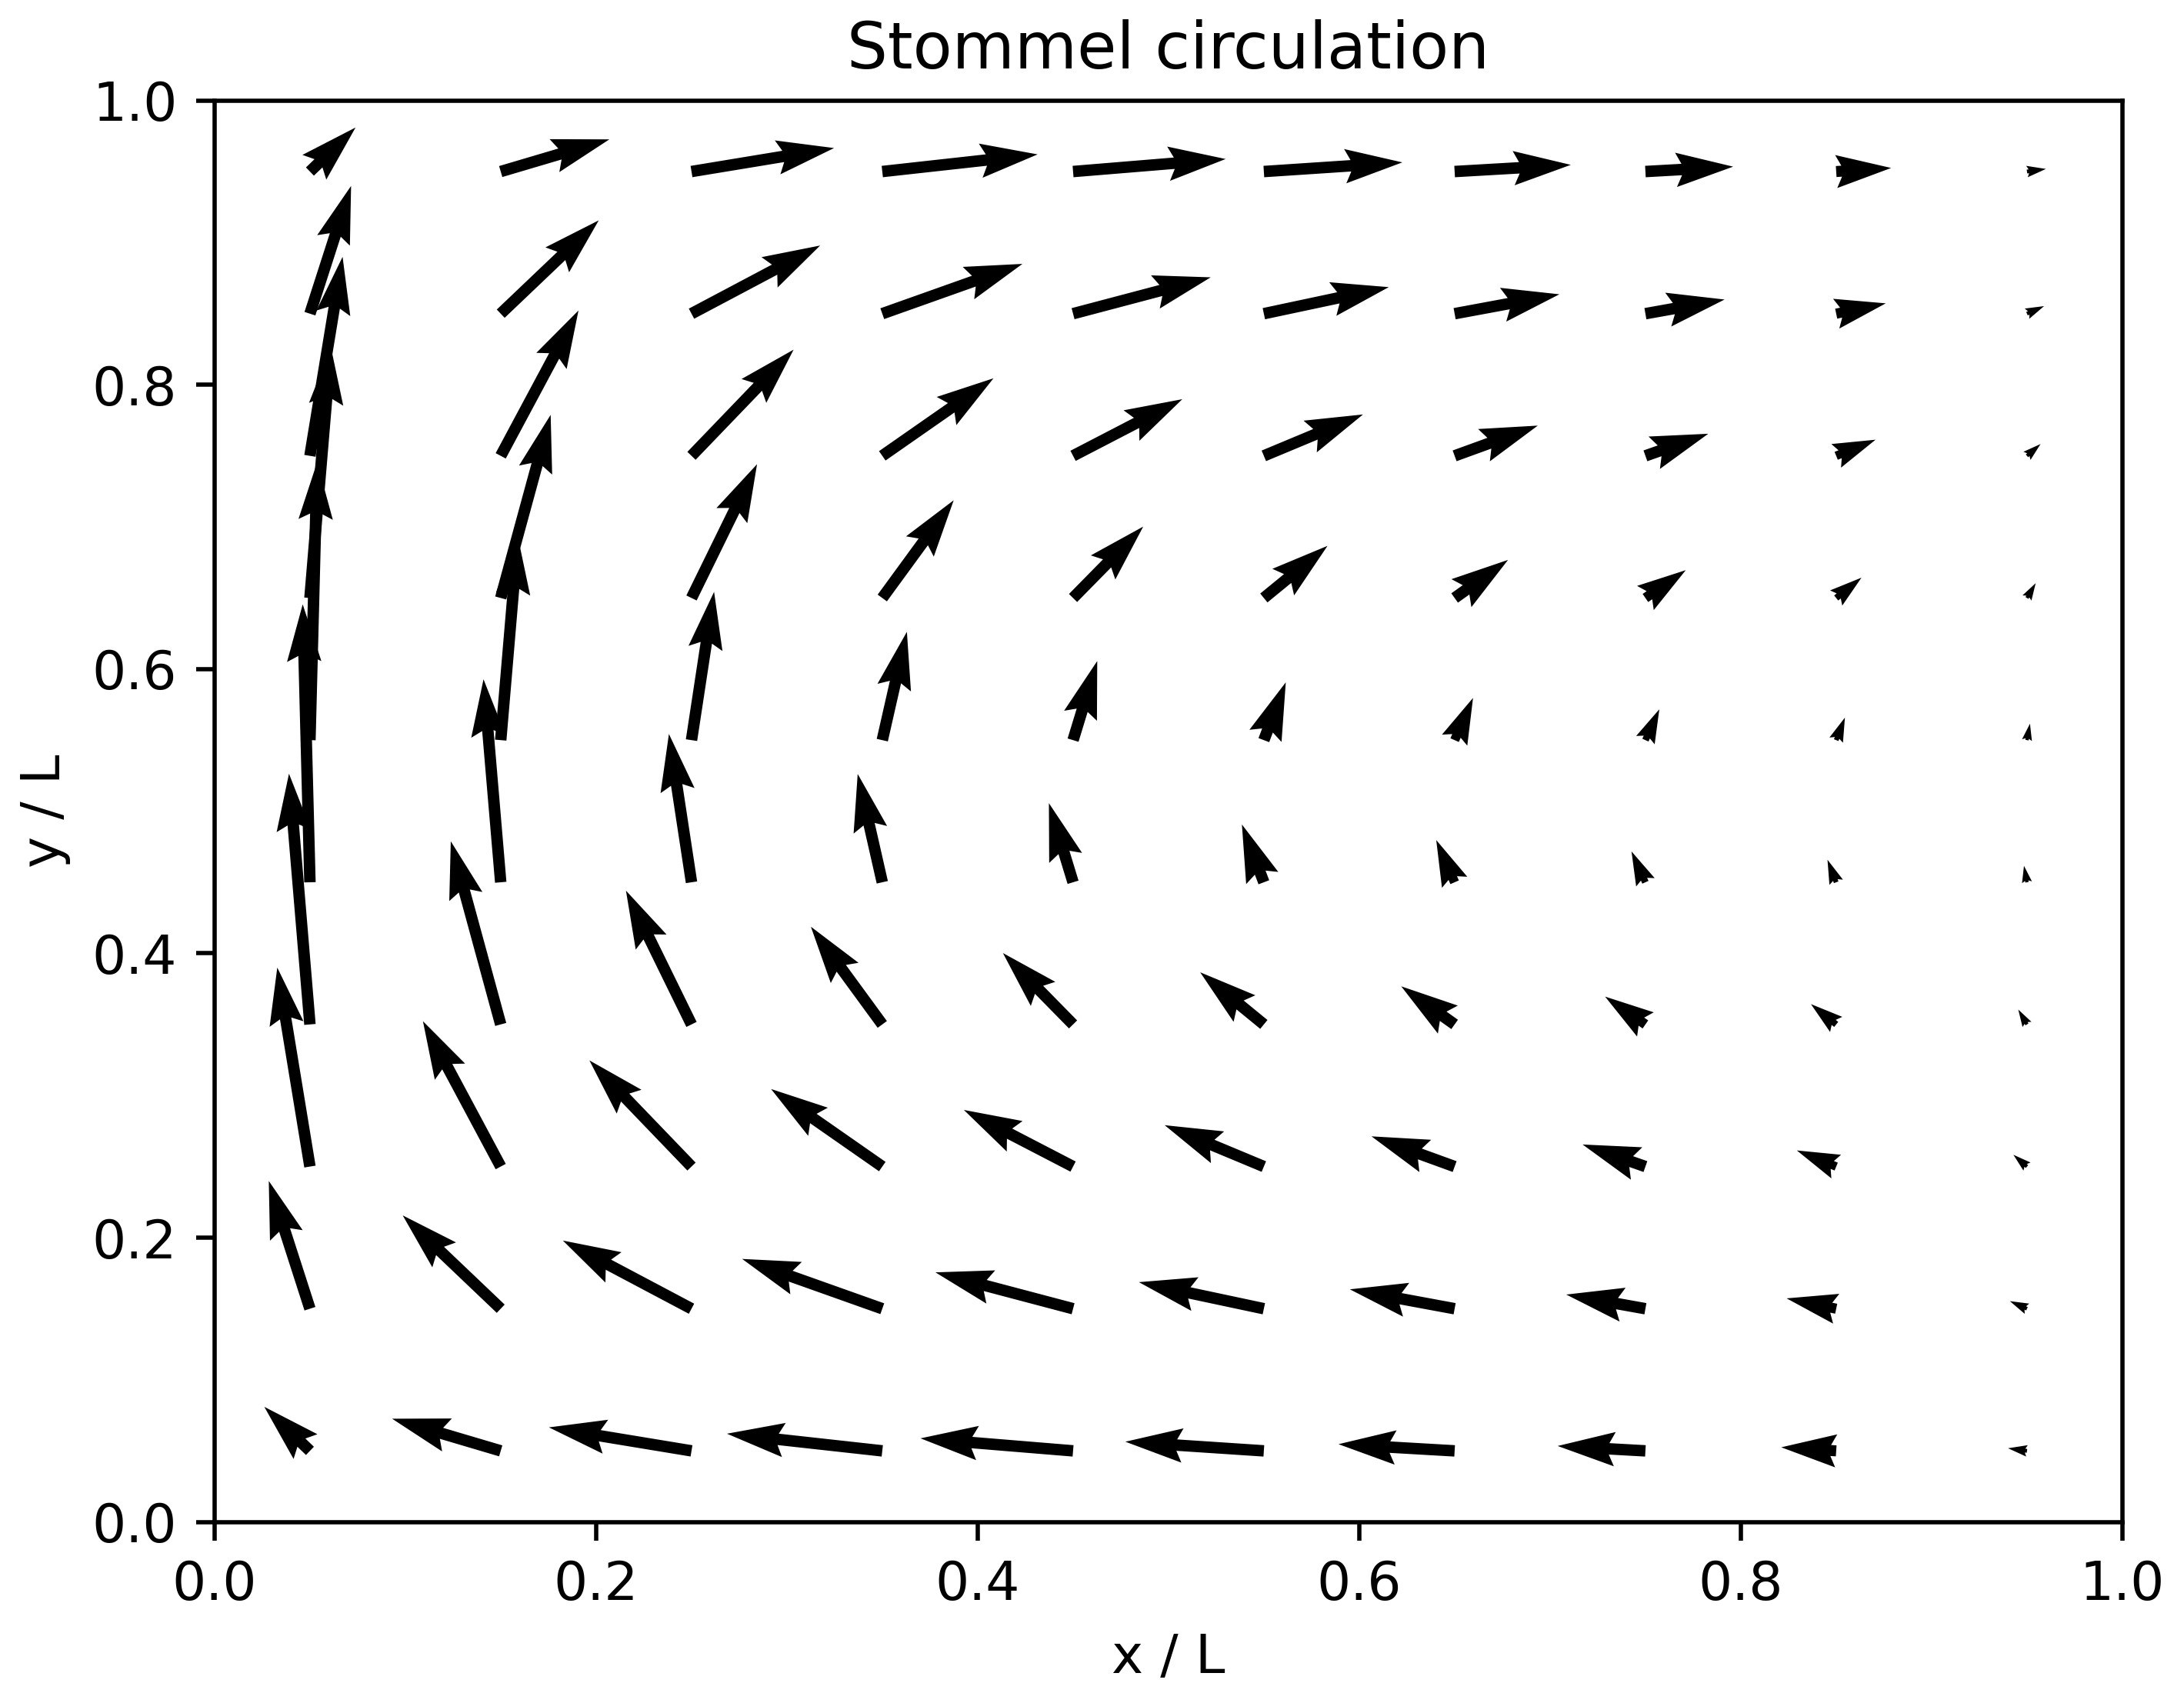
\includegraphics[width = 0.6\textwidth]{figs/stommel.png}
\caption{Visualisierung der Glg.en \eqref{eq:stommel_result_u} - \eqref{eq:stommel_result_v}.}
\label{fig:stommel}
\end{center}
\end{figure}

\section{Thermohaline Zirkulation}
\label{sec:thermohaline_zirkulation}\index{thermohaline Zirkulation}\index{Zirkulation!thermohaline}

\section{Seegangsvorhersage}
\label{sec:seegangsvorhersage}\index{Seegangsvorhersage}

\subsection{Prognostische Variablen}
\label{sec:prognostische_variablen_seegangsvorhersage}\index{prognostische Variable!Seegangsvorhersage}\index{Variable!prognostische!Seegangsvorhersage}\index{Seegangsvorhersage!prognostische Variablen}

\textit{Seegang}\index{Seegang} ist ein anderes Wort für Wasseroberflächenwellen\index{Wasseroberflächenwelle}. Die prognostische Variable, auf die dabei abgezielt wird, ist die Auslenkung der Wasseroberfläche
%
\begin{align}
h = h\left(x, y, t\right)
\end{align}
%
von der mittleren Position der Wasseroberfläche.\footnote{Es kann nicht einfach $h$ als Abweichung vom Geoid\index{Geoid} definiert werden, da hier noch die dynamische Topographie\index{dynamische Topographie}\index{Topographie!dynamische} überlagert wäre. Diese zählt nicht in die mit den Wellen verbundene Auslenkung hinein. Dementsprechend muss die Länge des Mittelungsintervalls gewählt werden.} In vielen Situationen ist $h$ keine Funktion der horizontalen Koordinaten, wie zum Beispiel im Falle von Brandung oder bei aufgewühlter See, da in diesen Fällen die Position der Wasseroberfläche nicht mehr eindeutig festgelegt ist. Solche Effekte werden später in Form von Energie dissipierenden Quelltermen berücksichtigt.

Es könnte nun als Satz prognosticher Gleichungen die in Absch. \ref{sec:flachwassergleichungen} hergeleiteten Flachwassergleichungen verwendet werden, eventuell mit einigen halb-empirischen Zusatztermen. Dies hat jedoch mehrere Nachteile:
%
\begin{itemize}
\item Um einen wesentlichen Anteil der Energie des Wellenfeldes\index{Wellenfeld} zu erfassen, wären ein sehr kleiner Zeitschritt und eine sehr feine räumliche Auflösung erforderlich.
\item Die Phasen der Wellen sind in den allermeisten Fällen nicht bekannt und auch nicht sehr relevant. Vielmehr sind Größen wie Richtung und Höhe der Wellen entscheidend.
\end{itemize}
%
Daher verwendet man zur Beschreibung von Wasseroberflächenwellen\index{Wasseroberflächenwelle} meistens eine Strahlungsübertragungsgleicung\index{Strahlungsübertragungsgleichung} (radiative transfer equation (\textsc{RTE}))\index{radiative transfer equation (\textsc{RTE})}\index{RTE (radiative transfer equation)}. Als prognostische Variable wird daher die spektrale Strahldichte\index{spektrale Strahldichte}\index{Strahldichte!spektrale}
%
\begin{align}
N = N\left(\mathbf{r}, \mathbf{k}, t\right)
\end{align}
%
verwendet. Hierbei sind $\mathbf{r}$ ein zweidimensionaler Ortsvektor und $\mathbf{k}$ ein zweidimensionaler Wellenvektor. Als Dispersionsrelation\index{Dispersionsrelation} $\omega = \omega\left(\mathbf{k}\right)$ wird diejenige der Sub-Poincaré-Wellen\index{Sub-Poincaré-Welle!Dispersionsrelation}\index{Dispersionsrelation!Sub-Poincaré-Welle}
%
\begin{align}
\omega^2 & = gk\tanh\left(kD\right) \Rightarrow \omega = \sqrt{gk\tanh\left(kD\right)},
\end{align}
%
verwendet, hierbei ist $D$ die mittlere Wassertiefe (Wassertiefe ohne Wellen). Hieraus folgen
%
\begin{align}
c_\text{ph} & = \frac{\omega}{k} = \sqrt{\frac{g\tanh\left(kD\right)}{k}},\\
c_\text{gr} & = \frac{1}{2\omega}\frac{\partial\omega^2}{\partial k} = \frac{1}{2\omega}\left[g\tanh\left(kD\right) + \frac{gkD}{\cosh^2\left(kD\right)}\right] = \frac{g\tanh\left(kD\right)}{2\omega}\left[1 + \frac{kD}{\sinh\left(kD\right)\cosh\left(kD\right)}\right]\nonumber\\
& = \frac{c_\text{ph}}{2}\left[1 + \frac{2kD}{2\sinh\left(kD\right)\cosh\left(kD\right)}\right] = \frac{c_\text{ph}}{2}\left[1 + \frac{2kD}{\sinh\left(2kD\right)}\right].
\end{align}
%
Alternativ könnte statt $\mathbf{k}$ auch $\left(\mathbf{e}_k, \omega\right)$ oder $\left(\theta, \omega\right)$ mit $\mathbf{e}_k = \left(\sin\left(\theta\right), \cos\left(\theta\right)\right)^T$ verwenden.

Die Gruppengeschwindigkeit wird als isotrop, aber nicht als homogen vorausgesetzt,
%
\begin{align}
c_\text{gr} = c_\text{gr}\left(\mathbf{k}\right),
\end{align}
%
die Ortsabhängigkeit entsteht über die Ortsabhängigkeit von $D$.

\subsection{Wave action equation}
\label{sec:wave_action_equation}\index{wave action equation}

Hieraus kann man eine spektrale Strahlungsflussdichte\index{spektrale Strahlungsflussdichte}\index{Strahlungsflussdichte!spektrale}
%
\begin{align}
N\left(\mathbf{r}, \mathbf{k}, t\right)\left(c_\text{gr}\left(\mathbf{r}, \mathbf{k}, t\right) + \mathbf{v}\left(\mathbf{r}, t\right)\right)
\end{align}
%
herleiten, hierbei ist $\mathbf{v} = \mathbf{v}\left(\mathbf{r}, t\right)$ die Stromgeschwindigkeit. Die Strahlungsübertragungsgleichung\index{Strahlungsübertragungsgleichung} ist eine Art Kontinuitätsgleichung für $N$, was konzeptionell mit der Energieerhaltung\index{Energieerhaltung} zusammenhängt:
%
\begin{center}
\doublebox{\parbox{0.8\textwidth}{
\begin{center}
\begin{align}
\frac{\partial N}{\partial t} + \nabla\cdot\left(N\left(\mathbf{r}, \mathbf{k}, t\right)c_\text{gr}\left(\mathbf{r}, \mathbf{k}\right)\right) & = S_\text{nl}\left(\mathbf{r}, \mathbf{k}, t\right) + S_\text{ws}\left(\mathbf{r}, \mathbf{k}, t\right) + S_\text{wc}\left(\mathbf{r}, \mathbf{k}, t\right)\nonumber\\
&   + S_\text{diss}\left(\mathbf{r}, \mathbf{k}, t\right) + S_\text{bd}\left(\mathbf{r}, \mathbf{k}, t\right)\label{eq:rte_water_surface}
\end{align}
\end{center}
}}
\end{center}
%
Hierbei wurden fünf zusätzliche Quellterme\index{Quellterm} aufgenommen:
%
\begin{itemize}
\item $S_\text{nl}\left(\mathbf{r}, \mathbf{k}, t\right)$ ist die Energiequelle, die aus nichtlinearen Effekten resultiert. Dieser Term ist besonders relevant für die Wechselwirkung von Skalen. Ein Beispiel ist die Entstehung langer Wellen (sogenannte \textit{Dünung}\index{Dünung}) aus der \textit{Windsee}\index{Windsee} (unmittelbar aus Windeinwirkung entstehende Wellen), welche aus kürzeren Wellen besteht, über upscaling\index{upscaling}.
\item $S_\text{ws}\left(\mathbf{r}, \mathbf{k}, t\right)$ ist die Energiequelle, die aus der Wechselwirkung mit dem Windfeld resultiert. Dies ist die Hauptenergiequelle des Wellenfeldes.
\item $S_\text{wc}\left(\mathbf{r}, \mathbf{k}, t\right)$ ist die Energiequelle, die aus der \textit{Gischt}\index{Gischt} (das sogenannte \textit{whitecapping}\index{whitecapping}) resultiert, dies ist ein dissipativer\index{Dissipation} und somit üblicherweise negativer Term.
\item $S_\text{diss}\left(\mathbf{r}, \mathbf{k}, t\right)$ ist die Energiequelle, die mit der inneren Reibung (Viskosität\index{Viskosität}) zusammenhängt. Da die Viskosität quadratisch stärker auf die kleineren Skalen wirkt, führt dieser Effekt dazu, dass Windsee\index{Windsee} schneller als Dünung\index{Dünung} dissipiert\index{Dissipation} wird.
\item $S_\text{bd}\left(\mathbf{r}, \mathbf{k}, t\right)$ ist die Energiequelle, die aus der Wechselwirkung mit der Bathymetrie\index{Bathymetrie} \textit{(bottom drag)}\index{bottom drag} zusammenhängt, auch dies ist ein dissipativer\index{Dissipation} und somit üblicherweise negativer Term.
\end{itemize}
%
Abhängig von der konkreten Situation können weitere Quellterme\index{Quellterm} aufgenommen werden. Glg. \eqref{eq:rte_water_surface} bezeichnet man auch als \textit{wave action equation}\index{wave action equation}.

\subsection{Diagnostische Variablen}
\label{sec:diagnostische_variablen}\index{diagnostische Variable!Seegangsvorhersage}\index{Variable!diagnostische!Seegangsvorhersage}\index{Seegangsvorhersage!diagnostische Variablen}

\subsection{Seegangsvorhersagemodelle}
\label{sec:seegangsvorhersagemodelle}\index{Seegangsvorhersagemodell}

Das gebräuchlichste Seegangsvorhersagemodell\index{Seegangsvorhersagemodell} ist \textsc{Wavewatch III}. Modelle, die sich an Glg. \eqref{eq:rte_water_surface} orientieren, sind sogenannte Seegangsvorhersagemodelle\index{Seegangsvorhersagemodell} dritter Generation. Sie lösen diese Gleichung auf einem Gitter und sind daher Gitterpunktmodelle, auch wenn sie gelegentlich als Spektralmodelle bezeichnet werden, da ihre prognostische Variable spektrale Bedeutung hat. Sie lösen meist Glg. \eqref{eq:rte_water_surface} in der Form Glg. , wobei an jedem Gitterpunkt ein spektrales richtungsabhängiges Gitter im $\left(\omega, \theta\right)-$Raum aufgespannt werden muss. Meist wird zusätzlich eine recht große Vielfalt an halb-empirischen Quelltermen $Q_i$ aufgenommen.

\part{Strahlung und Wolkenmikrophysik}
\label{part:strahlung_und_wolkenmikrophysik}

\chapter{\normalfont\textsc{Strahlungstransport}}
\label{chap:strahlungstransport}

Die zentrale Größe beim Strahlungstransport\index{Strahlungstransport} ist die spektrale Strahldichte\index{spektrale Strahldichte}\index{Strahldichte!spektrale} $L_\kappa\left(\mathbf{r}, \mathbf{n}, t\right)$, hierbei ist $\kappa$ die Wellenzahl und $\mathbf{n}$ ein Richtungsvektor. Aus ihr können u. a. Wärmeleistungsdichten\index{Wärmeleistungsdichte} abgeleitet werden.

\section{Berechnung der Streu- und Absorptionskoeffizienten}
\label{sec:berechnung_der_streu-_und_absorptionskoeffizienten}\index{Streukoeffizient}\index{Absorptionskoeffizient}

\section{Approximationen}
\label{sec:approximationen}

Die spektrale Strahldichte\index{spektrale Strahldichte}\index{Strahldichte!spektrale} hängt außer von der Zeit von sechs reellen Zahlen ab. Übliche Felder hängen von drei Koordinaten ab. Ein erstes Problem ist dementsprechend die Menge an Speicherplatz, die notwendig ist, um selbst einen sehr grob diskretisierten Strahlungszustand einer Atmosphäre abzuspeichern. Viel problematischer noch ist hingegen die Lösung der Strahlungsübertragungsgleichung. Daher sind rigorose Approximationen notwendig.

\subsection{Plan-parallele Atmosphäre}
\label{sec:pla-parallele-atmosphaere}\index{plan-parallele Atmosphäre}

Bei dieser Approximation geht man davon aus, dass die Atmosphäre innerhalb eines gewissen Gebietes horizontal homogen ist, die Eigenschaften also nur vertikal variieren. Dies ist durch die Tatsache motiviert, dass in der Atmosphäre auf großen Skalen horizontale Graienten mindestens zwei Größenordnungen kleiner sind als vertikale.

\subsection{Horizontale Entkopplung}
\label{sec:horizontale_entkopplung}\index{horizontale Entkopplung}

Bei dieser Approximation teilt man die Atmosphäre in unabhängige Säulen auf und schränkt dadurch die horizontale Wechselwirkung stark ein. Eine solche Säule kann jedoch aus verschiedenen Teilsäulen bestehen oder horizontale Wechselwirkungen können auf andere Weise innerhalb der Säulen parametrisiert werden. Bei steigender Rechenkapazität kann man die Bereiche mit horizontaler Wechselwirkung vergrößern, bis man im Grenzfäll die ganze Atmosphäre als eine einzige Säule ansieht.

\section{Atmosphärische Optik}
\label{sec:atmosphaerische_optik}\index{atmosphärische Optik}\index{Optik!atmosphärische}

\chapter{\normalfont\textsc{Wolkenmikrophysik}}
\label{chap:wolkenmikrophysik}\index{Wolkenmikrophysik}

\section{Köhler-Gleichung}
\label{sec:köhler-gleichung}\index{Köhler-Gleichung}

\section{Zirkulation um Kondensate}
\label{sec:zirkulation_um_kondensate}

\subsection{Laminare Umströmung}
\label{sec:laminare_umstroemung}\index{Kondensat!laminare Umströmung}\index{laminare Umströmung!von Kondensaten}\index{Umströmung!laminare!von Kondensaten}

Man stelle sich eine Kugel mit Radius $a$ vor, welche im Ursprung eines kartesischen Koordinatensystems zentriert ist. Man sucht nun nach Lösungen des imkompressiblen Gleichungssystems ohne Impulsadvektion
%
\begin{center}
\doublebox{\parbox{0.8\textwidth}{
\begin{center}
\begin{align}
\frac{\partial\mathbf{v}}{\partial t} &= -\frac{1}{\rho}\nabla p + \nu\Delta\mathbf{v},\label{eq:momentum_for_stokes}\\
\nabla\cdot\mathbf{v} &= 0\label{eq:incompressibility_stokes_fric}
\end{align}
\end{center}
}}
\end{center}
%
mit den Randbedingungen
%
\begin{center}
\doublebox{\parbox{0.8\textwidth}{
\begin{center}
\begin{align}
\lim_{\left|\mathbf{r}\right| \to \infty}\mathbf{v} &= U\mathbf{e}_z,\label{eq:stokes_fric_boundary_0}\\
\mathbf{v}\left(\left|\mathbf{r}\right| = a\right) &= \mathbf{0}.\label{eq:stokes_fric_boundary_1}
\end{align}
\end{center}
}}
\end{center}
%
lösen. Man beschränkt sich auf stationäre, also insbesondere laminare Lösungen. Damit wird die Impulsgleichung Glg. \eqref{eq:momentum_for_stokes} zu
%
\begin{align}
\nabla p &= \eta\Delta\mathbf{v}.\label{eq:momentum_for_stokes_mod}
\end{align}
%
Die Notation von $\mathbf{v}$ in Kugelkoordinaten lautet
%
\begin{align}
\mathbf{v} &= v_r\mathbf{e}_r + v_\theta\mathbf{e}_\theta + v_\phi\mathbf{e}_\phi.
\end{align}
%
Hierbei sind $\theta$ der Winkel gegenüber der z-Achse und $\phi$ der Winkel gegenüber der xz-Ebene. Stationäre Lösungen sind rotationssymmetrisch um die z-Achse, außerdem gilt
%
\begin{align}
v_\phi = 0.
\end{align}
%
Für die durch die Strömung entstehende Reibungskraft, welche auf die Kugel wirkt, gilt
%
\begin{align}
F = -2\pi a^2\int_0^\pi\left[p\cos\left(\theta\right) + \eta\sin\left(\theta\right)\frac{\partial v_\theta}{\partial r}\right]\sin\left(\theta\right)d\theta.
\end{align}
%
Solch eine Reibungskraft bezeichnet man als \textit{Stokes'sche Reibung}\index{Stokes'sche Reibung}\index{Reibung!Stokes'sche}. Dies teilt man auf in eine Kraft $F_p$, die durch den Druck $p$ entsteht, und in einer Kraft $F_v$, die durch die Scherung des Geschwindigkeitsfeldes entsteht
%
\begin{align}
F_p &\coloneqq -2\pi a^2\int_0^\pi p\cos\left(\theta\right)\sin\left(\theta\right)d\theta,\label{eq:stokes_friction_p}\\
F_v &\coloneqq -2\pi\eta a^2\int_0^\pi\frac{\partial v_\theta}{\partial r}\sin\left(\theta\right)^2d\theta.\label{eq:stokes_friction_v}
\end{align}
%
Damit gilt
%
\begin{align}
F = F_p + F_v.\label{eq:stokes_friction_split-up}
\end{align}
%
Nach den Feststellungen zu Beginn von Kap. \ref{chap:vorticity_und_divergenz} kann man $\mathbf{v}$ somit in der Form
%
\begin{align}
\mathbf{v} = \nabla\times\mathbf{A}
\end{align}
%
durch ein Geschwindigkeitspotential $\mathbf{A}$ darstellen. Nach Glg. \eqref{eq:rot_sphere} gilt
%
\begin{align}
\nabla\times\mathbf{A} &= \frac{A_\theta}{r}\mathbf{e}_\phi + \frac{A_\phi}{r\tan\left(\theta\right)}\mathbf{e}_r - \frac{A_\phi}{r}\mathbf{e}_\theta + \mathbf{e}_r\left(\frac{1}{r}\frac{\partial A_\phi}{\partial\theta} - \frac{1}{r\sin\left(\theta\right)}\frac{\partial A_\theta}{\partial\phi}\right)\nonumber\\
& + \mathbf{e}_\theta\left(\frac{1}{r\sin\left(\theta\right)}\frac{\partial A_r}{\partial\phi} - \frac{\partial A_\phi}{\partial r}\right) + \mathbf{e}_\phi\left(\frac{\partial A_\theta}{\partial r} - \frac{1}{r}\frac{\partial A_r}{\partial\theta}\right).
\end{align}
%
Aufgrund der Rotationssymmetrie um die z-Achse, ist $\mathbf{v}$ nicht von $\phi$ abhängig. Dies impliziert
%
\begin{align}
\nabla\times\mathbf{A} &= \frac{A_\theta}{r}\mathbf{e}_\phi + \frac{A_\phi}{r\tan\left(\theta\right)}\mathbf{e}_r - \frac{A_\phi}{r}\mathbf{e}_\theta + \mathbf{e}_r\frac{1}{r}\frac{\partial A_\phi}{\partial\theta} - \mathbf{e}_\theta\frac{\partial A_\phi}{\partial r} + \mathbf{e}_\phi\left(\frac{\partial A_\theta}{\partial r} - \frac{1}{r}\frac{\partial A_r}{\partial\theta}\right).
\end{align}
%
Durch Projektionen auf die ortsabhängigen Basiselemente der Kugelkoordinaten erhält man
%
\begin{align}
v_r &= \frac{A_\phi}{r\tan\left(\theta\right)} + \frac{1}{r}\frac{\partial A_\phi}{\partial\theta},\\
v_\theta &= -\frac{A_\phi}{r} - \frac{\partial A_\phi}{\partial r},\\
v_\phi &= \frac{A_\theta}{r} + \frac{\partial A_\theta}{\partial r} - \frac{1}{r}\frac{\partial A_r}{\partial\theta}.
\end{align}
%
Die Bedingung $v_\phi = 0$ kann man also durch $A_\theta = A_r = 0$ erfüllen, ohne die anderen Komponenten zu beeinträchtigen. Definiere
%
\begin{align}
\psi = \psi\left(r, \theta\right) \coloneqq -rA_\phi\sin\left(\theta\right),
\end{align}
%
dann gilt
%
\begin{center}
\doublebox{\parbox{0.8\textwidth}{
\begin{center}
\begin{align}
v_r &= -\frac{1}{r^2\sin\left(\theta\right)}\frac{\partial\psi}{\partial\theta}\label{eq:v_r_for_stokes_friction},\\
v_\theta &= \frac{1}{r\sin\left(\theta\right)}\frac{\partial\psi}{\partial r}.\label{eq:v_theta_for_stokes_friction}
\end{align}
\end{center}
}}
\end{center}
%
Die Rotation des Windfeldes lautet
%
\begin{align}
\nabla\times\mathbf{v} &= \frac{v_\theta}{r}\mathbf{e}_\phi + \frac{v_\phi}{r\tan\left(\theta\right)}\mathbf{e}_r - \frac{v_\phi}{r}\mathbf{e}_\theta + \mathbf{e}_r\frac{1}{r}\frac{\partial v_\phi}{\partial\theta} - \mathbf{e}_\theta\frac{\partial v_\phi}{\partial r} + \mathbf{e}_\phi\left(\frac{\partial v_\theta}{\partial r} - \frac{1}{r}\frac{\partial v_r}{\partial\theta}\right).
\end{align}
%
Mit $v_\phi = 0$ folgt hieraus
%
\begin{align}
\zetabi = \nabla\times\mathbf{v} &= \frac{v_\theta}{r}\mathbf{e}_\phi + \mathbf{e}_\phi\left(\frac{\partial v_\theta}{\partial r} - \frac{1}{r}\frac{\partial v_r}{\partial\theta}\right) = \mathbf{e}_\phi\left(\frac{\partial v_\theta}{\partial r} - \frac{1}{r}\frac{\partial v_r}{\partial\theta} + \frac{v_\theta}{r}\right).
\end{align}
%
Setzt man hier die Glg.en \eqref{eq:v_r_for_stokes_friction} - \eqref{eq:v_theta_for_stokes_friction} ein, erhält man
%
\begin{align}
\zetabi &= \nabla\times\mathbf{v} = \mathbf{e}_\phi\left(\frac{1}{r\sin\left(\theta\right)}\frac{\partial^2\psi}{\partial r^2} - \frac{1}{r^2\sin\left(\theta\right)}\frac{\partial\psi}{\partial r} - \frac{\cos\left(\theta\right)}{r^3\sin\left(\theta\right)^2}\frac{\partial\psi}{\partial\theta} + \frac{1}{r^3\sin\left(\theta\right)}\frac{\partial^2\psi}{\partial\theta^2} + \frac{1}{r^2\sin\left(\theta\right)}\frac{\partial\psi}{\partial r}\right)\nonumber\\
&= \mathbf{e}_\phi\left(\frac{1}{r\sin\left(\theta\right)}\frac{\partial^2\psi}{\partial r^2} - \frac{\cos\left(\theta\right)}{r^3\sin\left(\theta\right)^2}\frac{\partial\psi}{\partial\theta} + \frac{1}{r^3\sin\left(\theta\right)}\frac{\partial^2\psi}{\partial\theta^2}\right)\nonumber\\
&= \frac{\mathbf{e}_\phi}{r\sin\left(\theta\right)}\left(\frac{\partial^2\psi}{\partial r^2} - \frac{\cos\left(\theta\right)}{r^2\sin\left(\theta\right)}\frac{\partial\psi}{\partial\theta} + \frac{1}{r^2}\frac{\partial^2\psi}{\partial\theta^2}\right)\nonumber\\
&= \frac{\mathbf{e}_\phi}{r\sin\left(\theta\right)}\left[\frac{\partial^2}{\partial r^2} + \frac{\sin\left(\theta\right)}{r^2}\frac{\partial}{\partial\theta}\left(\frac{1}{\sin\left(\theta\right)}\frac{\partial}{\partial\theta}\right)\right]\psi \equiv \frac{\mathbf{e}_\phi}{r\sin\left(\theta\right)}E^2\psi
\end{align}
%
mit einem Differenzialoperator
%
\begin{align}
E^2 \coloneqq \frac{\partial^2}{\partial r^2} - \frac{1}{r^2\tan\left(\theta\right)}\frac{\partial}{\partial\theta} + \frac{1}{r^2}\frac{\partial^2}{\partial\theta^2} = \frac{\partial^2}{\partial r^2} + \frac{\sin\left(\theta\right)}{r^2}\frac{\partial}{\partial\theta}\left(\frac{1}{\sin\left(\theta\right)}\frac{\partial}{\partial\theta}\right).
\end{align}
%
Hieraus folgt, dass gilt
%
\begin{align}
\zetabi &= \nabla\times\left(\nabla\times\mathbf{A}\right) = \nabla\times\left[\nabla\times\left(A_\phi\mathbf{e}_\phi\right)\right] = -\nabla\times\left[\nabla\times\left(\frac{\psi}{r\sin\left(\theta\right)}\mathbf{e}_\phi\right)\right].
\end{align}
%
Für zweifach stetig differenzierbare Skalarfelder $\chi$ gilt also
%
\begin{align}
-\nabla\times\left[\nabla\times\left(\frac{\chi}{r\sin\left(\theta\right)}\mathbf{e}_\phi\right)\right] &= \frac{\mathbf{e}_\phi}{r\sin\left(\theta\right)}E^2\chi.
\end{align}
%
Glg. \eqref{eq:diff_op_rule_8} lautet
%
\begin{align}
\Delta\mathbf{v} &= \nabla\left(\nabla\cdot\mathbf{v}\right) - \nabla\times\left(\nabla\times\mathbf{v}\right) \stackrel{\text{Glg. \eqref{eq:incompressibility_stokes_fric}}}{=} -\nabla\times\left(\nabla\times\mathbf{v}\right) = -\nabla\times\zetabi.
\end{align}
%
Hiermit kann man die Impulsgleichung Glg. \eqref{eq:momentum_for_stokes_mod} in der Form
%
\begin{center}
\doublebox{\parbox{0.8\textwidth}{
\begin{center}
\begin{align}
\nabla p = -\eta\nabla\times\zetabi\label{eq:momentum_for_stokes_mod_mod}
\end{align}
\end{center}
}}
\end{center}
%
notieren. Wendet man hierauf nochmal die Rotation an, folgt
%
\begin{align}
0 = -\eta\nabla\times\left(\nabla\times\zetabi\right) = -\eta\nabla\times\left[\nabla\times\left(\frac{\mathbf{e}_\phi}{r\sin\left(\theta\right)}E^2\psi\right)\right] = \eta\frac{\mathbf{e}_\phi}{r\sin\left(\theta\right)}E^4\psi.
\end{align}
%
Man kann also
%
\begin{center}
\doublebox{\parbox{0.8\textwidth}{
\begin{center}
\begin{align}
E^4\psi = 0
\end{align}
\end{center}
}}
\end{center}
%
als Differenzialgleichung für $\psi$ verwenden. Aus der Randbedingung Glg. \eqref{eq:stokes_fric_boundary_1} folgt
%
\begin{align}
\frac{\partial\psi}{\partial r}\left(r = a\right) = \frac{\partial\psi}{\partial\theta}\left(r = a\right) = 0.
\end{align}
%
$\psi$ ist also konstant entlang der Kugeloberfläche, o. B. d. A. kann man als Randbedingung
%
\begin{align}
\psi\left(r = a\right) = 0
\end{align}
%
fordern. Die Randbedingung Glg. \eqref{eq:stokes_fric_boundary_0} lautet in Kugelkoordinaten
%
\begin{align}
\lim_{\left|\mathbf{r}\right| \to \infty}v_r &= U\cos\left(\theta\right),\\
\lim_{\left|\mathbf{r}\right| \to \infty}v_\theta &= -U\sin\left(\theta\right).
\end{align}
%
Dies impliziert für $\psi$ die Tatsache
%
\begin{align}
\lim_{\left|\mathbf{r}\right| \to \infty}\psi &= -\frac{Ur^2\sin\left(\theta\right)^2}{2}.
\end{align}
%
Der Druck soll in der Unendlichkeit gegen einen homogenen Hintergrunddruck $p_0$ konvergieren:
%
\begin{align}
\lim_{\left|\mathbf{r}\right| \to \infty}p &= p_0
\end{align}
%
Es gilt
%
\begin{align}
E^4\psi &= \left(\frac{\partial^2}{\partial r^2} - \frac{1}{r^2\tan\left(\theta\right)}\frac{\partial}{\partial\theta} + \frac{1}{r^2}\frac{\partial^2}{\partial\theta^2}\right)\left(\frac{\partial^2\psi}{\partial r^2} - \frac{1}{r^2\tan\left(\theta\right)}\frac{\partial\psi}{\partial\theta} + \frac{1}{r^2}\frac{\partial^2\psi}{\partial\theta^2}\right).
\end{align}
%
Man rechnet zunächst vorbereitend
%
\begin{align}
&\frac{\partial}{\partial r}\left(\frac{\partial^2\psi}{\partial r^2} - \frac{1}{r^2\tan\left(\theta\right)}\frac{\partial\psi}{\partial\theta} + \frac{1}{r^2}\frac{\partial^2\psi}{\partial\theta^2}\right) = \frac{\partial^3\psi}{\partial r^3} - \frac{1}{r^2\tan\left(\theta\right)}\frac{\partial^2\psi}{\partial r\partial\theta} + \frac{1}{r^2}\frac{\partial^3\psi}{\partial r\partial\theta^2} + \frac{2}{r^3\tan\left(\theta\right)}\frac{\partial\psi}{\partial\theta} - \frac{2}{r^3}\frac{\partial^2\psi}{\partial\theta^2},\nonumber\\
&\frac{\partial^2}{\partial r^2}\left(\frac{\partial^2\psi}{\partial r^2} - \frac{1}{r^2\tan\left(\theta\right)}\frac{\partial\psi}{\partial\theta} + \frac{1}{r^2}\frac{\partial^2\psi}{\partial\theta^2}\right) = \frac{\partial^4\psi}{\partial r^4} - \frac{1}{r^2\tan\left(\theta\right)}\frac{\partial^3\psi}{\partial r^2\partial\theta} + \frac{1}{r^2}\frac{\partial^4\psi}{\partial r^2\partial\theta^2} + \frac{2}{r^3\tan\left(\theta\right)}\frac{\partial^2\psi}{\partial r\partial\theta} - \frac{2}{r^3}\frac{\partial^3\psi}{\partial r\partial\theta^2}\nonumber\\
& + \frac{2}{r^3\tan\left(\theta\right)}\frac{\partial^2\psi}{\partial r\partial\theta} - \frac{2}{r^3}\frac{\partial^3\psi}{\partial r\partial\theta^2} - \frac{6}{r^4\tan\left(\theta\right)}\frac{\partial\psi}{\partial\theta} + \frac{6}{r^4}\frac{\partial^2\psi}{\partial\theta^2}\nonumber\\
&= \frac{\partial^4\psi}{\partial r^4} \textcolor{red}{- \frac{1}{r^2\tan\left(\theta\right)}\frac{\partial^3\psi}{\partial r^2\partial\theta}} + \textcolor{blue}{\frac{1}{r^2}\frac{\partial^4\psi}{\partial r^2\partial\theta^2}} + \frac{4}{r^3\tan\left(\theta\right)}\frac{\partial^2\psi}{\partial r\partial\theta} - \frac{4}{r^3}\frac{\partial^3\psi}{\partial r\partial\theta^2} - \frac{6}{r^4\tan\left(\theta\right)}\frac{\partial\psi}{\partial\theta} + \frac{6}{r^4}\frac{\partial^2\psi}{\partial\theta^2},
\end{align}
\begin{align}
&\frac{\partial}{\partial\theta}\left(\frac{\partial^2\psi}{\partial r^2} - \frac{\cos\left(\theta\right)}{r^2\sin\left(\theta\right)}\frac{\partial\psi}{\partial\theta} + \frac{1}{r^2}\frac{\partial^2\psi}{\partial\theta^2}\right) = \frac{\partial^3\psi}{\partial\theta\partial r^2} - \frac{\cos\left(\theta\right)}{r^2\sin\left(\theta\right)}\frac{\partial^2\psi}{\partial\theta^2} + \frac{1}{r^2}\frac{\partial^3\psi}{\partial\theta^3} + \frac{1}{r^2}\frac{\partial\psi}{\partial\theta} + \frac{\cos\left(\theta\right)^2}{r^2\sin\left(\theta\right)^2}\frac{\partial\psi}{\partial\theta}\nonumber\\
&\Rightarrow-\frac{1}{r^2\tan\left(\theta\right)}\frac{\partial}{\partial\theta}\left(\frac{\partial^2\psi}{\partial r^2} - \frac{\cos\left(\theta\right)}{r^2\sin\left(\theta\right)}\frac{\partial\psi}{\partial\theta} + \frac{1}{r^2}\frac{\partial^2\psi}{\partial\theta^2}\right)\nonumber\\
&= -\frac{1}{r^2\tan\left(\theta\right)}\frac{\partial^3\psi}{\partial\theta\partial r^2} + \frac{1}{r^4\tan\left(\theta\right)^2}\frac{\partial^2\psi}{\partial\theta^2} - \frac{1}{r^4\tan\left(\theta\right)}\frac{\partial^3\psi}{\partial\theta^3} - \frac{1}{r^4\tan\left(\theta\right)}\frac{\partial\psi}{\partial\theta} - \frac{1}{r^4\tan\left(\theta\right)^3}\frac{\partial\psi}{\partial\theta}\nonumber\\
&= \textcolor{red}{-\frac{1}{r^2\tan\left(\theta\right)}\frac{\partial^3\psi}{\partial\theta\partial r^2}} + \textcolor{brown}{\frac{1}{r^4\tan\left(\theta\right)^2}\frac{\partial^2\psi}{\partial\theta^2}} \textcolor{magenta}{- \frac{1}{r^4\tan\left(\theta\right)}\frac{\partial^3\psi}{\partial\theta^3}} \textcolor{green}{- \frac{\cos\left(\theta\right)}{r^4\sin\left(\theta\right)^3}\frac{\partial\psi}{\partial\theta}},
\end{align}
\begin{align}
&\frac{1}{r^2}\frac{\partial^2}{\partial\theta^2}\left(\frac{\partial^2\psi}{\partial r^2} - \frac{\cos\left(\theta\right)}{r^2\sin\left(\theta\right)}\frac{\partial\psi}{\partial\theta} + \frac{1}{r^2}\frac{\partial^2\psi}{\partial\theta^2}\right) = \frac{1}{r^2}\frac{\partial}{\partial\theta}\left(\frac{\partial^3\psi}{\partial\theta\partial r^2} - \frac{\cos\left(\theta\right)}{r^2\sin\left(\theta\right)}\frac{\partial^2\psi}{\partial\theta^2} + \frac{1}{r^2}\frac{\partial^3\psi}{\partial\theta^3} + \frac{1}{r^2}\frac{\partial\psi}{\partial\theta} + \frac{\cos\left(\theta\right)^2}{r^2\sin\left(\theta\right)^2}\frac{\partial\psi}{\partial\theta}\right)\nonumber\\
&= \frac{1}{r^2}\frac{\partial^4\psi}{\partial\theta^2\partial r^2} - \frac{\cos\left(\theta\right)}{r^4\sin\left(\theta\right)}\frac{\partial^3\psi}{\partial\theta^3} + \frac{1}{r^4}\frac{\partial^4\psi}{\partial\theta^4} + \frac{1}{r^4}\frac{\partial^2\psi}{\partial\theta^2} + \frac{\cos\left(\theta\right)^2}{r^4\sin\left(\theta\right)^2}\frac{\partial^2\psi}{\partial\theta^2}\nonumber\\
&+ \frac{1}{r^4}\frac{\partial^2\psi}{\partial\theta^2} + \frac{\cos\left(\theta\right)^2}{r^4\sin\left(\theta\right)^2}\frac{\partial^2\psi}{\partial\theta^2} - \frac{2\cos\left(\theta\right)}{r^4\sin\left(\theta\right)}\frac{\partial\psi}{\partial\theta} - \frac{2\cos\left(\theta\right)^3}{r^4\sin\left(\theta\right)^3}\frac{\partial\psi}{\partial\theta}\nonumber\\
&= \frac{1}{r^2}\frac{\partial^4\psi}{\partial\theta^2\partial r^2} - \frac{\cos\left(\theta\right)}{r^4\sin\left(\theta\right)}\frac{\partial^3\psi}{\partial\theta^3} + \frac{1}{r^4}\frac{\partial^4\psi}{\partial\theta^4} + \frac{2}{r^4\sin\left(\theta\right)^2}\frac{\partial^2\psi}{\partial\theta^2} - \frac{2\cos\left(\theta\right)}{r^4\sin\left(\theta\right)}\frac{\partial\psi}{\partial\theta} - \frac{2\cos\left(\theta\right)^3}{r^4\sin\left(\theta\right)^3}\frac{\partial\psi}{\partial\theta}\nonumber\\
&= \textcolor{blue}{\frac{1}{r^2}\frac{\partial^4\psi}{\partial\theta^2\partial r^2}} \textcolor{magenta}{- \frac{\cos\left(\theta\right)}{r^4\sin\left(\theta\right)}\frac{\partial^3\psi}{\partial\theta^3}} + \frac{1}{r^4}\frac{\partial^4\psi}{\partial\theta^4} + \textcolor{brown}{\frac{2}{r^4\sin\left(\theta\right)^2}\frac{\partial^2\psi}{\partial\theta^2}} \textcolor{green}{- \frac{2\cos\left(\theta\right)}{r^4\sin\left(\theta\right)^3}\frac{\partial\psi}{\partial\theta}}.
\end{align}
%
Somit erhält man
%
\begin{align}
E^4\psi &= \frac{\partial^4\psi}{\partial r^4} \textcolor{red}{- \frac{2}{r^2\tan\left(\theta\right)}\frac{\partial^3\psi}{\partial r^2\partial\theta}} + \textcolor{blue}{\frac{2}{r^2}\frac{\partial^4\psi}{\partial r^2\partial\theta^2}} + \frac{4}{r^3\tan\left(\theta\right)}\frac{\partial^2\psi}{\partial r\partial\theta} - \frac{4}{r^3}\frac{\partial^3\psi}{\partial r\partial\theta^2} - \frac{6}{r^4\tan\left(\theta\right)}\frac{\partial\psi}{\partial\theta} + \frac{6}{r^4}\frac{\partial^2\psi}{\partial\theta^2}\nonumber\\
& \textcolor{magenta}{- \frac{2}{r^4\tan\left(\theta\right)}\frac{\partial^3\psi}{\partial\theta^3}} \textcolor{green}{- \frac{3\cos\left(\theta\right)}{r^4\sin\left(\theta\right)^3}\frac{\partial\psi}{\partial\theta}} + \textcolor{brown}{\frac{2 + \cos\left(\theta\right)^2}{r^4\sin\left(\theta\right)^2}\frac{\partial^2\psi}{\partial\theta^2}} + \frac{1}{r^4}\frac{\partial^4\psi}{\partial\theta^4}\nonumber\\
&= \frac{\partial^4\psi}{\partial r^4} - \frac{2}{r^2\tan\left(\theta\right)}\frac{\partial^3\psi}{\partial r^2\partial\theta} + \frac{2}{r^2}\frac{\partial^4\psi}{\partial r^2\partial\theta^2} + \frac{4}{r^3\tan\left(\theta\right)}\frac{\partial^2\psi}{\partial r\partial\theta} - \frac{4}{r^3}\frac{\partial^3\psi}{\partial r\partial\theta^2}\nonumber\\
&- \frac{2}{r^4\tan\left(\theta\right)}\frac{\partial^3\psi}{\partial\theta^3} - \frac{3\cos\left(\theta\right)\left(1 + 2\sin\left(\theta\right)^2\right)}{r^4\sin\left(\theta\right)^3}\frac{\partial\psi}{\partial\theta} + \frac{2 + \cos\left(\theta\right)^2 + 6\sin\left(\theta\right)^2}{r^4\sin\left(\theta\right)^2}\frac{\partial^2\psi}{\partial\theta^2} + \frac{1}{r^4}\frac{\partial^4\psi}{\partial\theta^4}.
\end{align}
%
Die farblich markierten Terme wurden jeweils zusammengefasst. Dies impliziert mit Glg. \eqref{eq:v_theta_for_stokes_friction}
%
\begin{align}
v_\theta &= \frac{1}{r\sin\left(\theta\right)}\frac{\partial\psi}{\partial r} = \frac{1}{r\sin\left(\theta\right)}\frac{\partial}{\partial r}\left[\frac{Ua^2\sin^2\left(\theta\right)}{4}\left(-\frac{2r^2}{a^2} + \frac{3r}{a} - \frac{a}{r}\right)\right]\nonumber\\
&= \frac{1}{r}\left[\frac{Ua^2\sin\left(\theta\right)}{4}\left(-\frac{4r}{a^2} + \frac{3}{a} + \frac{a}{r^2}\right)\right] = \frac{Ua^2\sin\left(\theta\right)}{4}\left(-\frac{4}{a^2} + \frac{3}{ar} + \frac{a}{r^3}\right).
\end{align}
%
Hieraus folgt
%
\begin{align}
\frac{\partial v_\theta}{\partial r} &= -\frac{Ua^2\sin\left(\theta\right)}{4}\left(\frac{3}{ar^2} + \frac{3a}{r^4}\right).
\end{align}
%
Wertet man dies bei $r = a$ aus, folgt
%
\begin{align}
\frac{\partial v_\theta}{\partial r}\left(r = a\right) &= -\frac{Ua^2\sin\left(\theta\right)}{4}\left(\frac{3}{a^3} + \frac{3}{a^3}\right) = -\frac{6U\sin\left(\theta\right)}{4a} = -\frac{3U\sin\left(\theta\right)}{2a}.
\end{align}
%
Setzt man dies in Glg. \eqref{eq:stokes_friction_v} ein, erhält man
%
\begin{align}
F_v &= -2\pi\eta a^2\int_0^\pi-\frac{3U\sin\left(\theta\right)}{2a}\sin\left(\theta\right)^2d\theta = 3U\pi\eta a\int_0^\pi\sin\left(\theta\right)^3d\theta.
\end{align}
%
Man integriert nun
%
\begin{align}
\int_0^\pi\sin\left(\theta\right)^3d\theta &= \left[-\cos\left(\theta\right)\sin\left(\theta\right)^2\right]_0^\pi + 2\int_0^\pi\cos\left(\theta\right)^2\sin\left(\theta\right)d\theta\nonumber\\
&= 2\int_0^\pi\cos\left(\theta\right)^2\sin\left(\theta\right)d\theta = \frac{2}{3}\left[-\cos\left(\theta\right)^3\right]_0^\pi = \frac{2}{3}\left[\cos\left(\theta\right)^3\right]_\pi^0 = \frac{4}{3}.
\end{align}
%
Dies impliziert
%
\begin{align}
F_v &= 3U\pi\eta a\frac{4}{3} = 4U\pi\eta a.
\end{align}
%
Nun muss noch das Druckfeld bestimmt werden. Hierzu geht man aus von Glg. \eqref{eq:momentum_for_stokes_mod_mod}, man berechnet zunächst
%
\begin{align}
\nabla\times\zetabi &= \nabla\times\left[\mathbf{e}_\phi\frac{E^2\psi}{r\sin\left(\theta\right)}\right] \stackrel{\text{Glg. \eqref{eq:diff_op_rule_5}}}{=} -\mathbf{e}_\phi\times\nabla\frac{E^2\psi}{r\sin\left(\theta\right)} + \frac{E^2\psi}{r\sin\left(\theta\right)}\nabla\times\mathbf{e}_\phi.
\end{align}
%
Es gilt
%
\begin{align}
\nabla\frac{E^2\psi}{r\sin\left(\theta\right)} &= \nabla\left[\frac{1}{r\sin\left(\theta\right)}\left(\frac{\partial^2\psi}{\partial r^2} - \frac{\cos\left(\theta\right)}{r^2\sin\left(\theta\right)}\frac{\partial\psi}{\partial\theta} + \frac{1}{r^2}\frac{\partial^2\psi}{\partial\theta^2}\right)\right] = \nabla\left(\frac{1}{r\sin\left(\theta\right)}\frac{\partial^2\psi}{\partial r^2} - \frac{\cos\left(\theta\right)}{r^3\sin\left(\theta\right)^2}\frac{\partial\psi}{\partial\theta} + \frac{1}{r^3\sin\left(\theta\right)}\frac{\partial^2\psi}{\partial\theta^2}\right)\nonumber\\
&= \frac{\partial}{\partial r}\left(\frac{1}{r\sin\left(\theta\right)}\frac{\partial^2\psi}{\partial r^2} - \frac{\cos\left(\theta\right)}{r^3\sin\left(\theta\right)^2}\frac{\partial\psi}{\partial\theta} + \frac{1}{r^3\sin\left(\theta\right)}\frac{\partial^2\psi}{\partial\theta^2}\right)\mathbf{e}_r\nonumber\\
&+ \frac{1}{r}\frac{\partial}{\partial\theta}\left(\frac{1}{r\sin\left(\theta\right)}\frac{\partial^2\psi}{\partial r^2} - \frac{\cos\left(\theta\right)}{r^3\sin\left(\theta\right)^2}\frac{\partial\psi}{\partial\theta} + \frac{1}{r^3\sin\left(\theta\right)}\frac{\partial^2\psi}{\partial\theta^2}\right)\mathbf{e}_\theta\nonumber
\end{align}
\begin{align}
&= \left(\frac{1}{r\sin\left(\theta\right)}\frac{\partial^3\psi}{\partial r^3} - \frac{\cos\left(\theta\right)}{r^3\sin\left(\theta\right)^2}\frac{\partial^2\psi}{\partial r\partial\theta} + \frac{1}{r^3\sin\left(\theta\right)}\frac{\partial^3\psi}{\partial r\partial\theta^2} - \frac{1}{r^2\sin\left(\theta\right)}\frac{\partial^2\psi}{\partial r^2} + \frac{3\cos\left(\theta\right)}{r^4\sin\left(\theta\right)^2}\frac{\partial\psi}{\partial\theta} - \frac{3}{r^4\sin\left(\theta\right)}\frac{\partial^2\psi}{\partial\theta^2}\right)\mathbf{e}_r\nonumber\\
&+ \Bigg(\frac{1}{r^2\sin\left(\theta\right)}\frac{\partial^3\psi}{\partial \theta\partial r^2} - \frac{\cos\left(\theta\right)}{r^4\sin\left(\theta\right)^2}\frac{\partial^2\psi}{\partial\theta^2} + \frac{1}{r^4\sin\left(\theta\right)}\frac{\partial^3\psi}{\partial\theta^3} - \frac{\cos\left(\theta\right)}{r^2\sin\left(\theta\right)^2}\frac{\partial^2\psi}{\partial r^2} + \frac{1}{r^4\sin\left(\theta\right)}\frac{\partial\psi}{\partial\theta}\nonumber\\
&+ \frac{2\cos\left(\theta\right)^2}{r^4\sin\left(\theta\right)^3}\frac{\partial\psi}{\partial\theta} - \frac{\cos\left(\theta\right)}{r^4\sin\left(\theta\right)^2}\frac{\partial^2\psi}{\partial\theta^2}\Bigg)\mathbf{e}_\theta.
\end{align}
%
Hieraus folgt
%
\begin{align}
&-\mathbf{e}_\phi\times\nabla\frac{E^2\psi}{r\sin\left(\theta\right)}\nonumber\\
&= -\left(\frac{1}{r\sin\left(\theta\right)}\frac{\partial^3\psi}{\partial r^3} - \frac{\cos\left(\theta\right)}{r^3\sin\left(\theta\right)^2}\frac{\partial^2\psi}{\partial r\partial\theta} + \frac{1}{r^3\sin\left(\theta\right)}\frac{\partial^3\psi}{\partial r\partial\theta^2} - \frac{1}{r^2\sin\left(\theta\right)}\frac{\partial^2\psi}{\partial r^2} + \frac{3\cos\left(\theta\right)}{r^4\sin\left(\theta\right)^2}\frac{\partial\psi}{\partial\theta} - \frac{3}{r^4\sin\left(\theta\right)}\frac{\partial^2\psi}{\partial\theta^2}\right)\mathbf{e}_\theta\nonumber\\
&+ \Bigg(\frac{1}{r^2\sin\left(\theta\right)}\frac{\partial^3\psi}{\partial \theta\partial r^2} - \frac{\cos\left(\theta\right)}{r^4\sin\left(\theta\right)^2}\frac{\partial^2\psi}{\partial\theta^2} + \frac{1}{r^4\sin\left(\theta\right)}\frac{\partial^3\psi}{\partial\theta^3} - \frac{\cos\left(\theta\right)}{r^2\sin\left(\theta\right)^2}\frac{\partial^2\psi}{\partial r^2} + \frac{1}{r^4\sin\left(\theta\right)}\frac{\partial\psi}{\partial\theta}\nonumber\\
&+ \frac{2\cos\left(\theta\right)^2}{r^4\sin\left(\theta\right)^3}\frac{\partial\psi}{\partial\theta} - \frac{\cos\left(\theta\right)}{r^4\sin\left(\theta\right)^2}\frac{\partial^2\psi}{\partial\theta^2}\Bigg)\mathbf{e}_r\nonumber\\
&= \Bigg(\frac{1}{r^2\sin\left(\theta\right)}\frac{\partial^3\psi}{\partial \theta\partial r^2} \textcolor{brown}{- \frac{2\cos\left(\theta\right)}{r^4\sin\left(\theta\right)^2}\frac{\partial^2\psi}{\partial\theta^2}} + \frac{1}{r^4\sin\left(\theta\right)}\frac{\partial^3\psi}{\partial\theta^3} \textcolor{red}{- \frac{\cos\left(\theta\right)}{r^2\sin\left(\theta\right)^2}\frac{\partial^2\psi}{\partial r^2}} + \frac{1}{r^4\sin\left(\theta\right)}\frac{\partial\psi}{\partial\theta} + \textcolor{blue}{\frac{2\cos\left(\theta\right)^2}{r^4\sin\left(\theta\right)^3}\frac{\partial\psi}{\partial\theta}}\Bigg)\mathbf{e}_r\nonumber\\
&+ \left(-\frac{1}{r\sin\left(\theta\right)}\frac{\partial^3\psi}{\partial r^3} + \frac{\cos\left(\theta\right)}{r^3\sin\left(\theta\right)^2}\frac{\partial^2\psi}{\partial r\partial\theta} - \frac{1}{r^3\sin\left(\theta\right)}\frac{\partial^3\psi}{\partial r\partial\theta^2} + \textcolor{magenta}{\frac{1}{r^2\sin\left(\theta\right)}\frac{\partial^2\psi}{\partial r^2}} \textcolor{cyan}{- \frac{3\cos\left(\theta\right)}{r^4\sin\left(\theta\right)^2}\frac{\partial\psi}{\partial\theta}} + \textcolor{green}{\frac{3}{r^4\sin\left(\theta\right)}\frac{\partial^2\psi}{\partial\theta^2}}\right)\mathbf{e}_\theta
\end{align}
%
Mit
%
\begin{align}
\nabla\times\mathbf{e}_\phi &\stackrel{\text{Glg. \eqref{eq:rot_sphere}}}{=} \frac{1}{r\tan\left(\theta\right)}\mathbf{e}_r - \frac{1}{r}\mathbf{e}_\theta
\end{align}
%
folgt
%
\begin{align}
\frac{E^2\psi}{r\sin\left(\theta\right)}\nabla\times\mathbf{e}_\phi &= \frac{1}{r\sin\left(\theta\right)}\left[\frac{\partial^2\psi}{\partial r^2} - \frac{1}{r^2\tan\left(\theta\right)}\frac{\partial\psi}{\partial\theta} + \frac{1}{r^2}\frac{\partial^2\psi}{\partial\theta^2}\right]\left(\frac{1}{r\tan\left(\theta\right)}\mathbf{e}_r - \frac{1}{r}\mathbf{e}_\theta\right)\nonumber\\
&= \left(\frac{1}{r\sin\left(\theta\right)}\frac{\partial^2\psi}{\partial r^2} - \frac{\cos\left(\theta\right)}{r^3\sin\left(\theta\right)^2}\frac{\partial\psi}{\partial\theta} + \frac{1}{r^3\sin\left(\theta\right)}\frac{\partial^2\psi}{\partial\theta^2}\right)\left(\frac{1}{r\tan\left(\theta\right)}\mathbf{e}_r - \frac{1}{r}\mathbf{e}_\theta\right)\nonumber\\
&= \left(\frac{\cos\left(\theta\right)}{r^2\sin\left(\theta\right)^2}\frac{\partial^2\psi}{\partial r^2} - \frac{\cos\left(\theta\right)^2}{r^4\sin\left(\theta\right)^3}\frac{\partial\psi}{\partial\theta} + \frac{\cos\left(\theta\right)}{r^4\sin\left(\theta\right)^2}\frac{\partial^2\psi}{\partial\theta^2}\right)\mathbf{e}_r\nonumber\\
&- \left(\frac{1}{r^2\sin\left(\theta\right)}\frac{\partial^2\psi}{\partial r^2} - \frac{\cos\left(\theta\right)}{r^4\sin\left(\theta\right)^2}\frac{\partial\psi}{\partial\theta} + \frac{1}{r^4\sin\left(\theta\right)}\frac{\partial^2\psi}{\partial\theta^2}\right)\mathbf{e}_\theta\nonumber\\
&= \left(\textcolor{red}{\frac{\cos\left(\theta\right)}{r^2\sin\left(\theta\right)^2}\frac{\partial^2\psi}{\partial r^2}} \textcolor{blue}{- \frac{\cos\left(\theta\right)^2}{r^4\sin\left(\theta\right)^3}\frac{\partial\psi}{\partial\theta}} + \textcolor{brown}{\frac{\cos\left(\theta\right)}{r^4\sin\left(\theta\right)^2}\frac{\partial^2\psi}{\partial\theta^2}}\right)\mathbf{e}_r\nonumber\\
&+ \left(\textcolor{magenta}{-\frac{1}{r^2\sin\left(\theta\right)}\frac{\partial^2\psi}{\partial r^2}} + \textcolor{cyan}{\frac{\cos\left(\theta\right)}{r^4\sin\left(\theta\right)^2}\frac{\partial\psi}{\partial\theta}} \textcolor{green}{- \frac{1}{r^4\sin\left(\theta\right)}\frac{\partial^2\psi}{\partial\theta^2}}\right)\mathbf{e}_\theta.
\end{align}
%
Somit gilt
%
\begin{align}
&\nabla\times\zetabi\nonumber\\
&= \left(\frac{1}{r^2\sin\left(\theta\right)}\frac{\partial^3\psi}{\partial \theta\partial r^2} + \frac{1}{r^4\sin\left(\theta\right)}\frac{\partial^3\psi}{\partial\theta^3} + \frac{1}{r^4\sin\left(\theta\right)}\frac{\partial\psi}{\partial\theta} + \textcolor{blue}{\frac{\cos\left(\theta\right)^2}{r^4\sin\left(\theta\right)^3}\frac{\partial\psi}{\partial\theta}} \textcolor{brown}{- \frac{\cos\left(\theta\right)}{r^4\sin\left(\theta\right)^2}\frac{\partial^2\psi}{\partial\theta^2}}\right)\mathbf{e}_r\nonumber\\
&+ \left(-\frac{1}{r\sin\left(\theta\right)}\frac{\partial^3\psi}{\partial r^3} + \frac{\cos\left(\theta\right)}{r^3\sin\left(\theta\right)^2}\frac{\partial^2\psi}{\partial r\partial\theta} - \frac{1}{r^3\sin\left(\theta\right)}\frac{\partial^3\psi}{\partial r\partial\theta^2} \textcolor{cyan}{- \frac{2\cos\left(\theta\right)}{r^4\sin\left(\theta\right)^2}\frac{\partial\psi}{\partial\theta}} + \textcolor{green}{\frac{2}{r^4\sin\left(\theta\right)}\frac{\partial^2\psi}{\partial\theta^2}}\right)\mathbf{e}_\theta\nonumber\\
&= \left(\frac{1}{r^2\sin\left(\theta\right)}\frac{\partial^3\psi}{\partial \theta\partial r^2} + \frac{1}{r^4\sin\left(\theta\right)}\frac{\partial^3\psi}{\partial\theta^3} + \frac{1}{r^4\sin\left(\theta\right)^3}\frac{\partial\psi}{\partial\theta} - \frac{\cos\left(\theta\right)}{r^4\sin\left(\theta\right)^2}\frac{\partial^2\psi}{\partial\theta^2}\right)\mathbf{e}_r\nonumber\\
&+ \left(-\frac{1}{r\sin\left(\theta\right)}\frac{\partial^3\psi}{\partial r^3} + \frac{\cos\left(\theta\right)}{r^3\sin\left(\theta\right)^2}\frac{\partial^2\psi}{\partial r\partial\theta} - \frac{1}{r^3\sin\left(\theta\right)}\frac{\partial^3\psi}{\partial r\partial\theta^2} - \frac{2\cos\left(\theta\right)}{r^4\sin\left(\theta\right)^2}\frac{\partial\psi}{\partial\theta} + \frac{2}{r^4\sin\left(\theta\right)}\frac{\partial^2\psi}{\partial\theta^2}\right)\mathbf{e}_\theta.
\end{align}
%
Die farblich markierten Terme heben sich jeweils paarweise (in Teilen) gegenseitig auf. Dies impliziert für die durch den Druck entstehende Reibungskraft laut Glg. \eqref{eq:stokes_friction_p}
%
\begin{align}
F_p &= -2\pi a^2\int_0^\pi-\frac{3\eta aU\cos\left(\theta\right)}{2a^2}\cos\left(\theta\right)\sin\left(\theta\right)d\theta = \pi\int_0^\pi 3\eta aU\cos\left(\theta\right)\cos\left(\theta\right)\sin\left(\theta\right)d\theta\nonumber\\
&= 3\eta aU\pi\int_0^\pi\cos^2\left(\theta\right)\sin\left(\theta\right)d\theta = -3\eta aU\pi\left[\frac{1}{3}\cos\left(\theta\right)^3\right]_0^\pi = 2\eta aU\pi.
\end{align}
%
Somit gilt laut Glg. \eqref{eq:stokes_friction_split-up} für die Reibungskraft
%
\begin{center}
\doublebox{\parbox{0.8\textwidth}{
\begin{center}
\begin{align}
F = 6\pi a\eta U.\label{eq:stokes_friction}
\end{align}
\end{center}
}}
\end{center}
%
Setzt man dies mit der Gewichtskraft
%
\begin{align}
F_g = mg = \frac{4}{3}\pi a^3\rho_l'g\label{eq:gravity_on_condensate}
\end{align}
%
gleich, erhält man
%
\begin{center}
\doublebox{\parbox{0.8\textwidth}{
\begin{center}
\begin{align}
v_\text{sink} = \frac{F}{6\pi a\eta} = \frac{4\pi a^3\rho_l'g}{18\pi a\rho_h'\nu} = \frac{2\pi a^2\rho_l'g}{9\pi\rho_h'\nu}\label{eq:sink_stokes}
\end{align}
\end{center}
}}
\end{center}
%
als Formel für die Gleichgewichts-Sinkgeschwindigkeit $v_\text{sink}$.

\subsection{Turbulente Umströmung}
\label{sec:turbulente_umstroemung}

Bei turbulenter Umströmung ist die das Kondensat umgebende Zirkulation in aperiodischer Weise zeitabhängig. Hierbei ist die Reibungskraft $F$ proportional zum Quadrat der Geschwindigkeit $U$,
%
\begin{align}
F = \frac{1}{2}c_w\pi a^2\rho_h'U^2,\label{eq:turbulent_friction}
\end{align}
%
wobei $c_w \geq 0$ eine von der Form des umströmten Objektes abhängige Konstante, der sogenannte \textit{$c_w-$Wert}\index{$c_w-$Wert}, ist. Im Englischen bezeichnet man diese Größe als \textit{drag coefficient}\index{drag coefficient} $c_d$. Setzt man dies mit der Gewichtskraft laut Glg. \eqref{eq:gravity_on_condensate} gleich, erhält man
%
\begin{align}
\frac{1}{2}c_w\pi a^2\rho_h'v_\text{sink}^2 &= \frac{4}{3}\pi a^3\rho_l'g \Leftrightarrow v_\text{sink}^2 = \frac{8a\rho_l'g}{3\rho_h'c_w}
\end{align}
\begin{center}
\doublebox{\parbox{0.8\textwidth}{
\begin{center}
\begin{align}
\Leftrightarrow v_\text{sink} = \sqrt{\frac{8a\rho_l'g}{3\rho_h'c_w}}\label{eq:sink_turb}
\end{align}
\end{center}
}}
\end{center}
%
als Formel für die Gleichgewichts-Sinkgeschwindigkeit $v_\text{sink}$.

\subsubsection{Zusammengesetzte Formel für die Sinkgeschwindigkeit}
\label{sec:zusammengesetzte_formel_für_die_sinkgeschwindigkeit}

Kleine Kondensate werden laminar umströmt, größere turbulent. Der Parameter $\alpha\in\left[0, 1\right]$ beschreibe den Anteil von Turbulenz in der Reibungskraft $F$, also
%
\begin{align}
F = \alpha F_\text{turbulent} + \left(1 - \alpha\right)F_\text{laminar}.
\end{align}
%
Setzt man hier die Glg.en \eqref{eq:stokes_friction} und \eqref{eq:turbulent_friction} ein, erhält man
%
\begin{align}
F = \alpha\frac{1}{2}c_w\pi a^2\rho_h'U^2 + \left(1 - \alpha\right)6\pi a\rho_h'\nu U.
\end{align}
%
Setzt man dies mit der Gewichtskraft laut Glg. \eqref{eq:gravity_on_condensate} gleich, erhält man unter der Annahme $\alpha \not= 0$

\begin{align}
\left(1 - \alpha\right)6\pi a\rho_h'\nu v_\text{sink} + \alpha\frac{1}{2}c_w\pi a^2\rho_h'v_\text{sink}^2 &= \frac{4}{3}\pi a^3\rho_l'g\nonumber\\
\Leftrightarrow\alpha\frac{1}{2}c_w\pi a\rho_h'v_\text{sink}^2 + \left(1 - \alpha\right)6\pi\rho_h'\nu v_\text{sink} - \frac{4}{3}\pi a^2\rho_l'g &= 0\nonumber\\
\Leftrightarrow\alpha c_w\pi a\rho_h'v_\text{sink}^2 + \left(1 - \alpha\right)12\pi\rho_h'\nu v_\text{sink} - \frac{8\pi a^2\rho_l'g}{3} &= 0\nonumber\\
\Leftrightarrow\alpha c_w\pi av_\text{sink}^2 + \left(1 - \alpha\right)12\pi\nu v_\text{sink} - \frac{8\pi a^2\rho_l'g}{3\rho_h'} &= 0\nonumber\\
\Leftrightarrow \pi av_\text{sink}^2 + \frac{\left(1 - \alpha\right)}{\alpha c_w}12\pi \nu v_\text{sink} - \frac{8\pi a^2\rho_l'g}{3\alpha\rho_h'c_w} &= 0\nonumber\\
\Leftrightarrow v_\text{sink}^2 + \frac{\left(1 - \alpha\right)}{a\alpha c_w}12\nu v_\text{sink} - \frac{8a\rho_l'g}{3\alpha\rho_h'c_w} &= 0.
\end{align}
%
Es ist zu erwarten, dass der Übergang von laminarer zu turbulenter Reibung entscheidend von der Reynolds-Zahl
%
\begin{align}
R \coloneqq \frac{U^2a^2}{\nu Ua} = \frac{Ua}{\nu}
\end{align}
%
abhängt. Man nimmt nun an, dass der Übergang von laminarer zu turbulenter Reibung bei einer kritischen Reynolds-Zahl $R_k$ erfolgt. Um die Gleichgewichts-Sinkgeschindigkeit zu bestimmen, kann man wie folgt vorgehen:
%
\begin{enumerate}
\item Berechne $v_\text{sink}$ aus Glg. \eqref{eq:sink_stokes}.
\item Berechne hieraus die Reynoldszahl $R$.
\item Wenn das Ergebnis nicht größer als $R_k$ ist, $R \leq R_k$, gilt $\alpha = 0$ und das Ergebnis liegt bereits vor. Dabei kann bei Kugeln von $R_k = 10$ ausgegangen werden.
\item Andernfalls gilt $\alpha = 1$, dann verwende \eqref{eq:sink_turb} zur Bestimmung der Gleichgewichts-Sinkgeschwindigkeit. Dabei kann bei Kugeln von $c_w = 1$ ausgegangen werden.
\end{enumerate}

\section{Wachstum von Kondensaten}
\label{sec:wachstum_von_kondensaten}

\subsection{Koagulation}
\label{sec:koagulation}\index{Koagulation}

\subsubsection{Bergeron-Findeisen-Prozess}
\label{sec:bergeron-findeisen-prozess}\index{Bergeron-Findeisen-Prozess}

\subsection{Koaleszenz}
\label{sec:koaleszenz}\index{Koaleszenz}

\section{Zerbrechen von Wassertropfen}
\label{sec:zerbrechen_von_wassertropfen}

\subsection{Innere Zirkulation}
\label{sec:innere_zirkulation}

\subsection{Oszillationen}
\label{sec:oszillationen}

\subsection{Instabilitäten}
\label{sec:instabilitäten}

\part{Numerik}
\label{part:numerik}\index{Numerik}

\chapter{\normalfont\textsc{Grundkonzepte der Numerik}}
\label{chap:grundkonzepte_der_numerik}\index{Numerik!Grundkonzepte}\index{Grundkonzepte!Numerik}

Ein Wettermodell ist eine Kopie der Atmosphäre. In ihm sind alle Felder und Differenzialoperatoren durch diskretisierte Versionen ersetzt, da man nur endlich viel Information abspeichern kann. Man schreibt für einen Differenzialoperator $D$ eine Ersetzung
%
\begin{align}
D\to D', 
\end{align}
%
analog für atmosphärische Zustände
%
\begin{align}
Z\to Z'.
\end{align}
%
Anschließend legt man eine Dynamik fest, also ein Verfahren
%
\begin{align}
Z'\left(t\right)\stackrel{D'}{\to}Z'\left(t + \Delta t\right)
\end{align}
%
zur Bestimmung der Zeitentwicklung der Modellatmosphäre mit dem Ziel, die Zustandstrajektorie des Modells möglichst nah an diejenige der realen Atmosphäre zu bringen. Hierzu definiert man einen Abstand
%
\begin{align}
\left|Z - Z'\right|\geq 0.
\end{align}
%
Wettervorhersage hat den folgenden Arbeitsablauf:
%
\begin{enumerate}
\item Beobachtung des Zustandes der Atmosphäre.
\item Bestimmung des Anfangszustandes des Modells.
\item Integration des Modells.
\end{enumerate}
%
Dabei entstehen aus folgenden Gründen Fehler:
%
\begin{enumerate}
\item Der Anfangszustand wurde nicht vollständig beobachtet.
\item Der Anfangszustand wurde fehlerhaft beobachtet.
\item Die herrschenden Gleichungen sind Gleichungen der statistischen Physik und gelten somit nicht exakt.
\item Das Modell kann weniger Information abspeichern als die reale Atmosphäre.
\item Die Dynamik des Modells ist von der der realen Atmosphäre verschieden.
\item Es existieren Rundungsfehler durch die endliche Rechnergenauigkeit.
\item Der Rechner macht Fehler.
\end{enumerate}
%
\section{Grundbegriffe von Diskretisierungen}
\label{sec:grundbegiffe_von_diskretisierunge}\index{Diskretisierung}

Die Lösung einer Differenzialgleichung sei mit $F$ bezeichnet und die Lösung einer diskretisierten Version der Gleichung mit $F_d$. Ein numerisches Verfahren heißt genau dann \textit{konsistent}\index{Konsistenz!eines numerischen Verfahrens}, wenn die Lösung des Schemas bei kleiner werdenden $\Delta x$ und $\Delta t$ gegen die Lösung der Differenzialgleichung konvergiert, also $\lim\limits_{\Delta\to 0}F_d = F$ in obigen Begriffen. Eine Diskretisierung heißt genau dann \textit{selbstkonsistent}\index{Selbstkonsistenz!eines numerischen Verfahrens}, wenn alle Erhaltungsgrößen des kontinuierlichen Systems auch Erhaltungsgrößen des diskretisierten Systems sind. Dies lässt sich auch auf Näherungen übertragen. Ein Schema heißt genau dann \textit{stabil}, wenn die berechnete Lösung für alle Zeiten beschränkt ist, wenn also ein $C>0$ existiert mit $|F_d|<C$ für alle $t\geq t_0$ mit $t_0$ als Startzeitpunkt. \textit{Lineare Instabilität} entsteht bereits bei linearen Differenzialgleichungen, wohingegen \textit{nichtlineare Instabilität} nur bei nichtlinearen Differenzialgleichungen entstehen kann.

\section{Finite Differenzen}
\label{sec:finite_differenzen}\index{Differenz!finite}\index{finite Differenz}

Sei eine unendlich oft differenzierbare Funktion $f:\mathbb{R}\to\mathbb{R}$ gegeben. Mittels einer Taylorreihe kann man schreiben
%
\begin{align}
f\left(x + \Delta x\right) = f\left(x\right) + \Delta xf'\left(x\right) + \frac{f''\left(x\right)}{2!}\Delta x^2 + \frac{f'''\left(x\right)}{3!}\Delta x^3 + \dotsc\label{eq:taylor_links}
\end{align}
%
und
%
\begin{align}
f\left(x - \Delta x\right) = f\left(x\right) - \Delta xf'\left(x\right) + \frac{f''\left(x\right)}{2!}\Delta x^2 - \frac{f'''\left(x\right)}{3!}\Delta x^3 + \dotsc\label{eq:taylor_rechts}
\end{align}
%
Subtrahiert man beide Gleichungen, erhält man
%
\begin{align}
f\left(x + \Delta x\right) - f\left(x - \Delta x\right) = 2\Delta xf'\left(x\right) + R', 
\end{align}
%
wobei der Rest $R'$ für die Terme dritter und höherer Ordnung steht. Dies ergibt umgestellt
%
\begin{align}
f'\left(x\right) = \frac{f\left(x + \Delta x\right) - f\left(x - \Delta x\right)}{2\Delta x} + R, \label{eq:approx_derivative_zentral}
\end{align}
%
wobei $R$ ein Polynom in $\Delta x$ mit der geringsten Potenz 2 ist, man sagt, dass durch \eqref{eq:approx_derivative_zentral} eine Approximation zweiter Ordnung der Ableitung gegeben ist und schreibt anstelle von $R$ das Symbol $\mathcal{O}\left(\Delta x^2\right)$. Man nennt diese Art, Ableitungen zu approximieren, zentrale Differenzenquotienten. Ein einseitiger Differenzenquotient, zum Beispiel
%
\begin{align}
f'\left(x\right) \approx\frac{f\left(x + \Delta x\right) - f\left(x\right)}{\Delta x}
\end{align}
%
ist ebenfalls eine geeignete Approximation, jedoch konvergiert dies nur in erster Ordnung, wie leicht durch Umstellen von Glg. \eqref{eq:taylor_links} ersichtlich ist. Desto höher die Ordnung, desto besser, da die Genauigkeit einer Taylor-Entwicklung ja mit der Ordnung anwächst. Aus diesem Grund werden, soweit möglich, zentrale räumliche Differenzenquotienten verwendet. Man kann aus den Glg.en \eqref{eq:taylor_links} und \eqref{eq:taylor_rechts} auch eine Approximation für die zweite Ableitung einer Funktion herleiten:
%
\begin{align}
f\left(x + \Delta x\right) + f\left(x - \Delta x\right)& = 2f\left(x\right) + f''\left(x\right)\Delta x^2 + \mathcal{O}\left(\Delta x^4\right)\nonumber\\
\Leftrightarrow f''\left(\Delta x\right) & = \frac{f\left(x + \Delta x\right) - 2f\left(x\right) + f\left(x - \Delta x\right)}{\Delta x^2} + \mathcal{O}\left(\Delta x^2\right)
\end{align}
%
Hat man beispielsweise eine Funktion $f\left(x\right) = A\sin\left(kx\right)$ gegeben, so gilt $f' = Ak\cos\left(kx\right)$, Glg. \eqref{eq:approx_derivative_zentral} ergibt jedoch
%
\begin{align}
f' &\approx& \frac{A}{2\Delta x}\left(\sin\left(kx + k\Delta x\right) - \sin\left(kx - k\Delta x\right)\right) = \frac{A}{\Delta x}\cos\left(kx\right)\sin\left(k\Delta x\right) = \frac{\sin\left(k\Delta x\right)}{k\Delta x}f'.
\end{align}
%
Hieran sieht man, dass die Approximation, wie erwartet, gegen den richtigen Wert der Ableitung konvergiert, falls $\Delta x$ gegen Null geht (es gilt $\lim\limits_{\alpha\to 0}\frac{\sin\left(\alpha\right)}{\alpha} = 1$ nach der Regel von L'Hospital). Schreibt man für $k = \frac{2\pi}{\lambda}$ mit $\lambda$ als Wellenlänge und setzt $\Delta x = \lambda/2$ ein, so ergibt der zentrale Differenzenquotient immer $f' = 0$. Hinreichend lange Wellen ($\lambda\gg 2\Delta x$) werden jedoch gut aufgelöst.

\section{Ebene Spektralmethode}
\label{sec:ebene_spektralmethode}

\section{Sphärische Spektralmethode}
\label{sec:sphärische_spektralmethode}

Sei $\psi = \psi\left(\varphi, \lambda, z\right)$ ein Skalarfeld. Da die in Absch. \ref{sec:kugelflaechenfunktionen} vorgestellten Kugelflächenfunktionen\index{Kugelflächenfunktion} eine vollständige Orthonormalbasis\index{vollständige Orthonormalbasis}\index{Orthonormalbasis!vollständige} auf Kugelschalen\index{Kugelschale} bilden, ist es möglich, die horizontale Abhängigkeit von $\psi$ durch diesen Satz an Funktionen auszudrücken:
%
\begin{align}
\psi\left(\varphi, \lambda, z\right) = \sum_{l = 0}^\infty\sum_{m = -l}^l\newtilde{\psi}_{l, m}\left(z\right)Y_{l, m}\left(\varphi, \lambda\right)
\end{align}
%
Die Definition der Kugelflächenfunktionen\index{Kugelflächenfunktion} Glg. \eqref{eq:def_spherical_harmonics} wird hier in geographischen Koordinaten\index{geographische Koordinaten}\index{Koordinaten!geographische} formuliert:
%
\begin{align}
Y_{l, m}\left(\varphi, \lambda\right) = \sqrt{\frac{2l + 1}{4\pi}\frac{\left(l - m\right)!}{\left(l + m\right)!}}P_{l, m}\left(\sin\left(\varphi\right)\right)\exp\left(im\lambda\right)
\end{align}

\begin{figure}
\begin{center}
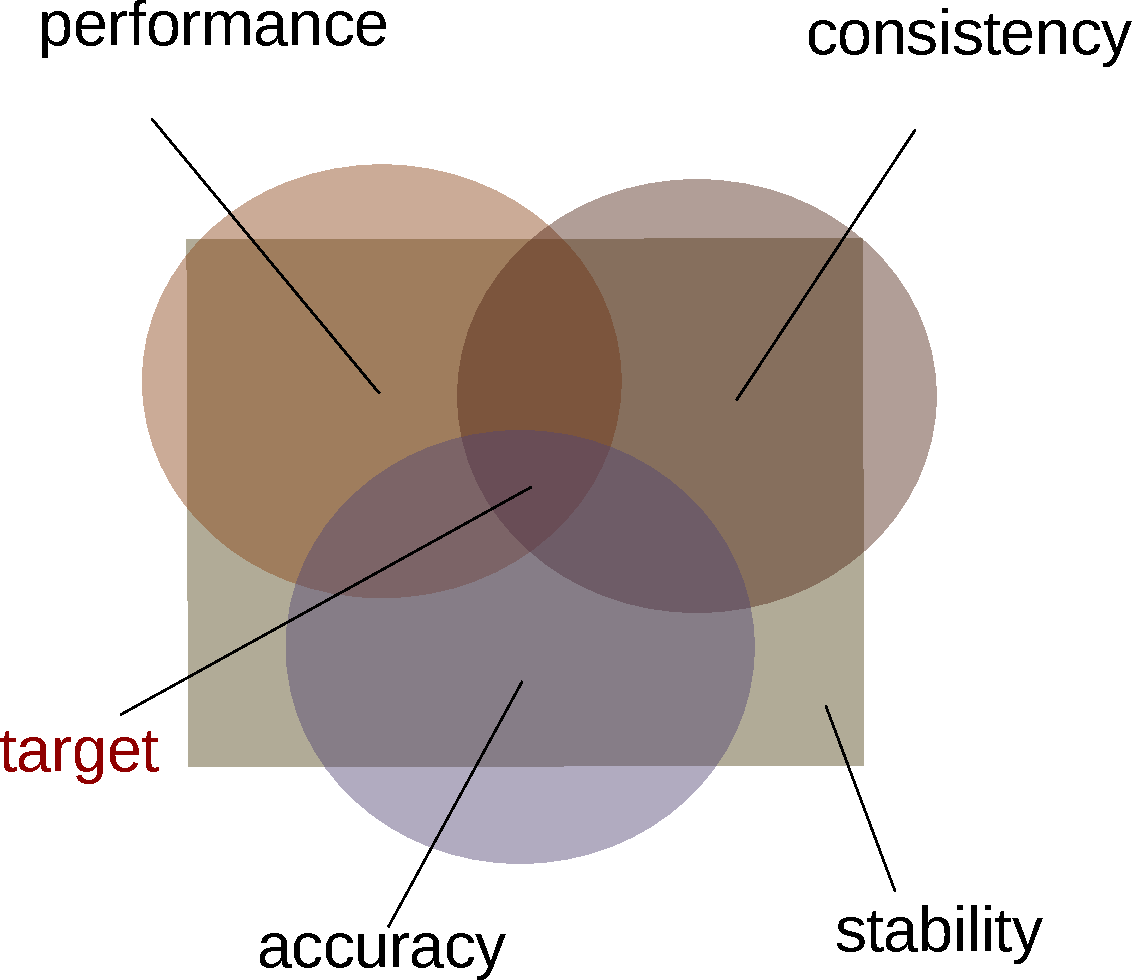
\includegraphics[width = 0.5\textwidth]{figs/discretizations.pdf}
\caption{Mengen von Diskretisierungen.}
\label{fig:discretization_sets}
\end{center}
\end{figure}

\chapter{\normalfont\textsc{Zeitschrittverfahren}}
\label{chap:zeitschrittverfahren}\index{Zeitschrittverfahren}

Sei $\psi: A \subseteq \mathbb{R}^3 \times \mathbb{R} \to \mathbb{R}^n$ der atmosphärische Zustandsvektor. Alle fundamentalen physikalischen Gesetze sind erster Ordnung in der Zeit, daher kann man schreiben
%
\begin{align}
\frac{d\psi}{dt} = F\left(\psi\right),
\end{align}
%
wobei $F$ die Physik enthält. Diskretisiert man dies auf ein zeitliches Gitter $n\Delta t$ mit $n \in \mathbb{Z}$ und interpoliert zwischen zwei Zeitschritten $n$, $n + l$, erhält man
%
\begin{align}
\psi_{n + l} - \psi_{n} = \int_{n\Delta t}^{\left(n + l\right)\Delta t}F\left(\psi\right)dt.
\end{align}
%
Die Anzahl der dabei involvierten Zeitschritte ist $l + 1$. Man kann nun das Integral auf der rechten Seite auf vielfälitge Art und Weise diskretisieren. Das explizite Euler-Verfahren\index{explizites Eueler-Verfahren}\index{Euler-Verfahren!explizites} ergibt sich mit $l = 1$ über die Näherung
%
\begin{align}
\int_{n\Delta t}^{\left(n + 1\right)\Delta t}F\left(\psi\right)dt \approx F\left(\psi_{n}\right)\Delta t
\end{align}
%
mit $\psi_{n} \coloneqq \psi\left(n\Delta t\right)$. Das implizite Euler-Verfahren\index{implizites Eueler-Verfahren}\index{Euler-Verfahren!implizites} hingegen erhält man über
%
\begin{align}
\int_{n\Delta t}^{\left(n + 1\right)\Delta t}F\left(\psi\right)dt \approx F\left(\psi_{n + 1}\right)\Delta t
\end{align}

In diesem Kapitel soll verständlich gemacht werden, wie sich die zeitliche Disktretisierung einer linearen Differenzialgleichung auf die Dispersionsrelation und die Stabilität einer Wellenlösung auswirken kann. Es wird die lineare Advektionsgleichung 
%
\begin{align}
\frac{\partial f}{\partial t} + U\frac{\partial f}{\partial x} = 0\label{eq:test_lineare_instab}
\end{align}
%
betrachtet mit $U\not = 0$ als homogener Advektionsgeschwindigkeit und $f$ als irgendeiner Teilcheneigenschaft. Die analytische Lösung lautet in der komplexen Schreibweise
%
\begin{align}
f = \exp\left(i\left(kx - \omega t\right)\right), 
\end{align}
%
setzt man dies ein folgt $-i\omega + Uik = 0$, also als Dispersionsrelation
%
\begin{align}
\omega = Uk.
\end{align}
%
Phasen- und Gruppengeschwindigkeit sind also gleich $U$. Nun werden Ort und Zeit diskretisiert, man schreibt $f_l^{(m)} = f\left(l\Delta x, m\Delta t\right)$ und setzt an 
%
\begin{align}
f_{l}^{(m)} = e^{Cm\Delta t}e^{i\left(kl\Delta x - \omega m\Delta t\right)}\label{eq:ansatz_time_stepping_1d_analysis}
\end{align}
%
mit $f_{l}^{(0)} = e^{ikl\Delta x}$ als Anfangszustand. Es sollen $C$ und die Dispersion $\omega\left(k\right)$ bestimmt werden.

\section{Rein explizite Verfahren}
\label{sec:rein_explizite_verfahren}

\subsection{Explizites Euler-Verfahren}
\label{sec:explizites_euler-verfahren}\index{explizites Euler-Verfahren}\index{Euler-Verfahren!explizites}

Zunächst wird folgende Diskretisierung untersucht:
%
\begin{align}
\frac{f_l^{(m + 1)} - f_l^{(m)}}{\Delta t} + U\frac{f_{l + 1}^{(m)} - f_{l - 1}^{(m)}}{2\Delta x} = 0
\end{align}
%
Dies bezeichnet man als \textit{explizites Euler-Verfahren}.\index{Euler-Verfahren!explizites}\index{explizites Euler-Verfahren} Einsetzen ergibt
%
\begin{align}
\frac{e^{C\Delta t}e^{-i\omega\Delta t} - 1}{\Delta t} + U \frac{e^{ik\Delta x} - e^{-ik\Delta x}}{2\Delta x} = \frac{e^{C\Delta t}\cos\left(\omega\Delta t\right) - ie^{C\Delta t}\sin\left(\omega\Delta t\right) - 1}{\Delta t} + \frac{iU\sin\left( k\Delta x\right)}{\Delta x} = 0.
\end{align}
%
Der Realteil ist
%
\begin{align}
e^{C\Delta t}\cos\left(\omega\Delta t\right) = 1, 
\end{align}
%
hieraus folgt i. A. $C> 0$, es liegt Instabilität vor. Hierbei handelt es sich um \index{Instabilität!lineare}\index{lineare Instabilität}\textit{lineare Instabilität}, da Glg. \eqref{eq:test_lineare_instab} linear in $f$ ist. Der Imaginärteil ist
%
\begin{align}
e^{C\Delta t}\sin\left(\omega\Delta t\right) = \frac{U\Delta t\sin\left(k\Delta x\right)}{\Delta x}.
\end{align}
%
Hieraus folgt
%
\begin{align}
\tan\left(\omega\Delta t\right) = \frac{U\Delta t\sin\left(k\Delta x\right)}{\Delta x}, 
\end{align}
%
also die Dispersion
%
\begin{align}
\omega\left(k\right) = \frac{1}{\Delta t}\arctan\left(\frac{U\Delta t\sin\left(k\Delta x\right)}{\Delta x}\right).
\end{align}
%
$\lambda$ sei die Wellenlänge, also $k = \frac{2\pi}{\lambda}$. Für $\lambda\gg \Delta x$ gilt $\sin\left(k\Delta x\right) \approx k\Delta x$, also $\omega \approx \frac{1}{\Delta t}\arctan\left(Uk\Delta t\right)$. Im Fall $U\Delta t\ll \lambda$, also $Uk\Delta t\ll 1$, ist $\omega \approx \frac{1}{\Delta t}U\Delta t k = Uk$ wie im kontinuierlichen Fall. Lange Wellen werden bei hinreichend kleinem Zeitschritt also gut aufgelöst. Bei der kürzesten aufgelösten Welle $\lambda = 2\Delta x$ jedoch folgt $\omega = \frac{1}{\Delta t}\arctan\left(\frac{U\Delta t\sin\pi}{\Delta x}\right) = 0$, die Welle ist also stationär. Abb. \ref{fig:disp_1d} zeigt die Dispersionsrelation für den Fall $U = 10$ m/s. Man erkennt, dass Wellen mit $k\leq \frac{1}{\Delta x}$, also $\lambda\geq 2\pi\Delta x$ anständig simuliert werden.

\begin{figure}
\begin{center}
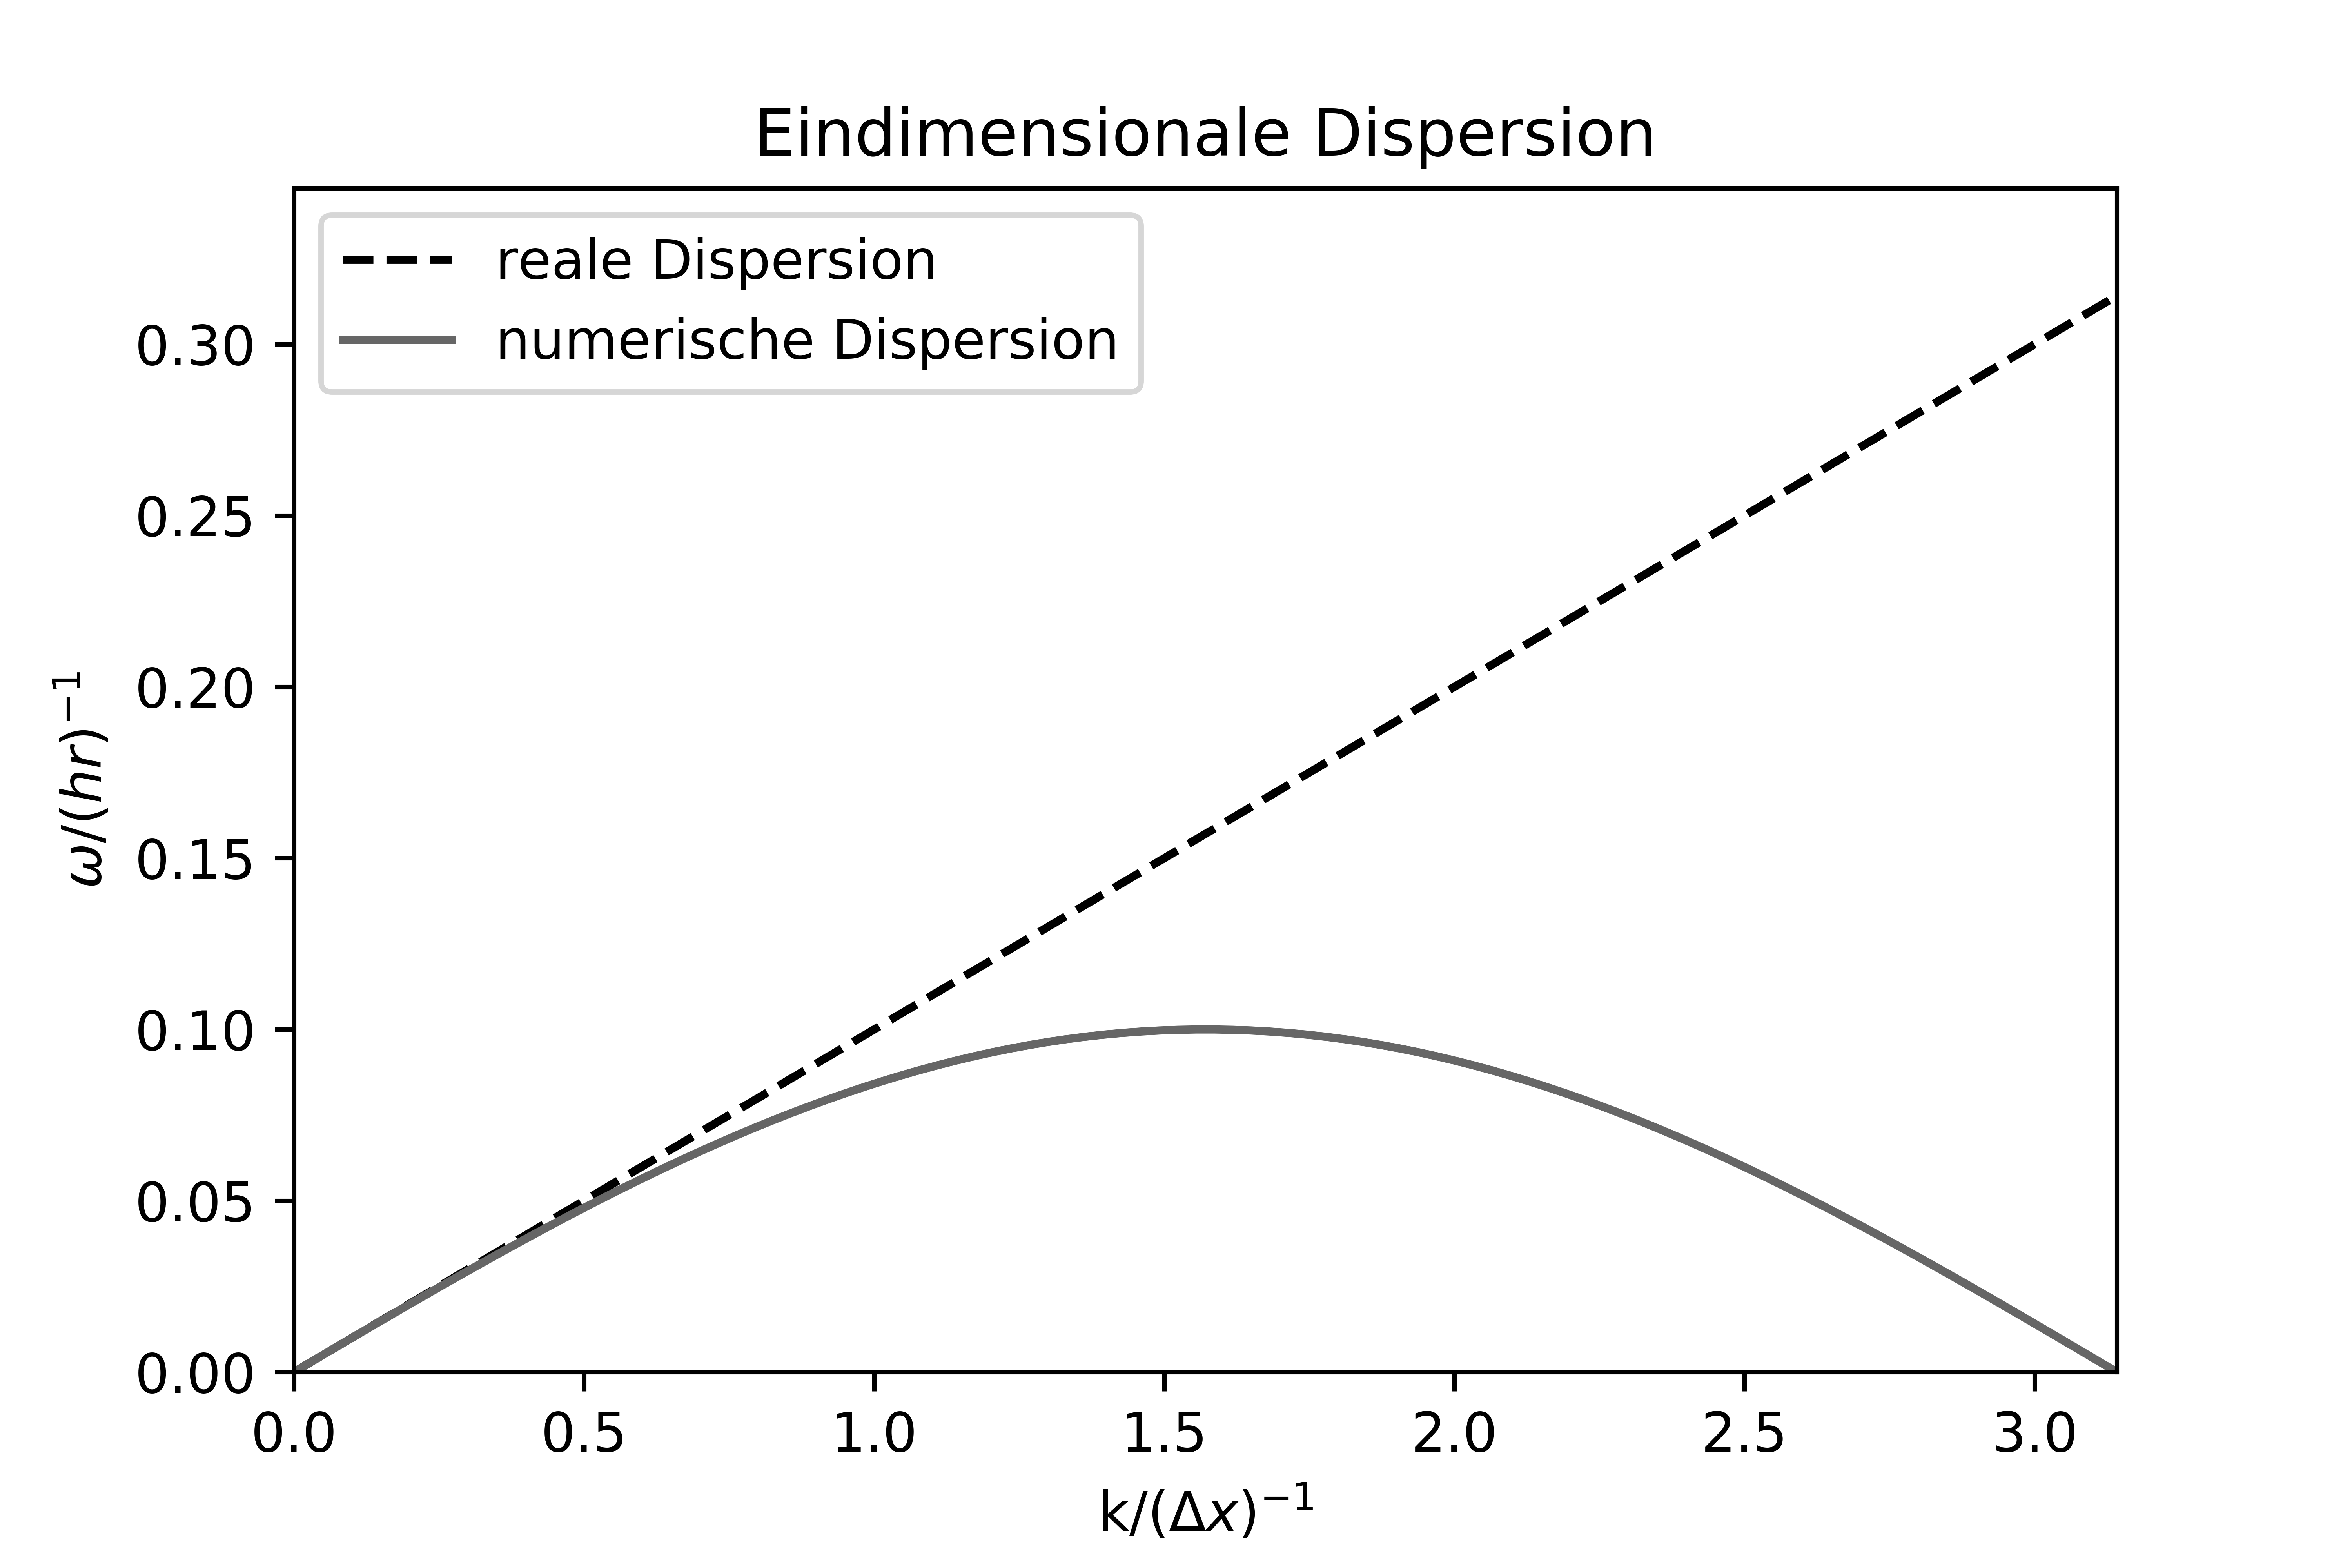
\includegraphics[width = 0.6\textwidth]{figs/dispersion_1d.png}
\caption{Numerische und tatsächliche Dispersion in der 1D-Advektionsgleichung. Es wurde mit $U = 10$ m/s gerechnet, für $\Delta t$ wurde ein sehr geringer Wert eingesetzt. Man beachte den Vorzeichenwechsel der Gruppengeschwindigkeit. Wellen mit der geringsten aufgelösten Wellenlänge $2\Delta x$ sind stationär. Wellen mit einer Wellenlänge $\geq 6\Delta x$ werden gut simuliert.}
\label{fig:disp_1d}
\end{center}
\end{figure}

\subsection{Leapfrog-Verfahren}
\label{sec:leapfrog-verfahren}\index{Leapfrog-Verfahren}

Verwendet man einen zentralen zeitlichen Differenzenquotienten, schreibt also
%
\begin{align}
\frac{f_l^{(m + 2)} - f_l^{(m)}}{2\Delta t} + U\frac{f_{l + 1}^{(m + 1)} - f_{l - 1}^{(m + 1)}}{2\Delta x} = 0, 
\end{align}
%
so ergibt dies eingesetzt
%
\begin{align}
\frac{e^{2C\Delta t}e^{-2i\omega\Delta t} - 1}{2\Delta t} + U \frac{e^{ik\Delta x}e^{C\Delta t}e^{-i\omega\Delta t} - e^{-ik\Delta x}e^{C\Delta t}e^{-i\omega\Delta t}}{2\Delta x} & = 0 \nonumber\\
\Leftrightarrow \frac{e^{C\Delta t}e^{-i\omega\Delta t} - e^{-C\Delta t}e^{i\omega\Delta t}}{2\Delta t} + U \frac{e^{ik\Delta x} - e^{-ik\Delta x}}{2\Delta x} & = 0.
\end{align}
%
Der Realteil ergibt
%
\begin{align}
e^{C\Delta t}\cos\left(\omega\Delta t\right) = e^{-C\Delta t}\cos\left(\omega\Delta t\right).
\end{align}
%
Das bedeutet $C = 0$, die Lösung ist also stabil. Der Imaginärteil wird zu
%
\begin{align}
\frac{\sin\left(\omega\Delta t\right)}{2\Delta t}\left(e^{-C\Delta t} + e^{C\Delta t}\right) = \frac{\sin\left(\omega\Delta t\right)}{\Delta t} = U\frac{\sin\left(k\Delta x\right)}{\Delta x}.
\end{align}
%
Daraus folgt
%
\begin{align}
\sin\left(\omega\Delta t\right) = U\frac{\Delta t}{\Delta x}\sin\left(k\Delta x\right)\Rightarrow\omega = \frac{1}{\Delta t}\arcsin\left[\frac{U\Delta t}{\Delta x}\sin\left(k\Delta x\right)\right], 
\end{align}
%
also eine andere Dispersionsrelation als im expliziten Fall. Allgemein scheint die Stabilität der Lösung aus dem Realteil ersichtlich zu sein, während die Dispersion aus dem Imaginärteil zu folgen scheint. Schemata sind weiterhin entweder stabil ($C \leq 0$), labil ($C > 0$) oder bedingt stabil (stabil für hinreichend kleine $\Delta t$). Dies wird vom Zeitschrittverfahren beeinflusst. Der Optimalfall ist $C = 0$, er ergibt sich für das Leapfrogverfahren, daher ist dieses Verfahren das geeignetste.

\subsection{Runge-Kutta-Verfahren}
\label{sec:runge-kutta-verfahren}\index{Runge-Kutta-Verfahren}

\section{CFL-Kriterium}
\label{sec:cfl-kriterium}\index{CFL-Kriterium}\index{Courant-Friedrichs-Lewy-Kriterium}

Das \textit{Courant-Friedrichs-Lewy-Kriterium (CFL-Kriterium)} ist eine Beschränkung des maximalen Zeitschrittes bei expliziten Verfahren. Sei $u$ die Phasengeschwindigkeit der am schnellsten propagierenden Welle. Man definiert die \textit{Courant-Zahl}\index{Courant-Zahl} oder auch \textit{CFL-Zahl}\index{CFL-Zahl} $c$ durch
%
\begin{align}
c \coloneqq \frac{u\Delta t}{\Delta x}.
\end{align}
%
Das CFL-Kriterium lautet

\begin{center}
\doublebox{\parbox{0.8\textwidth}{
\begin{center}
Das explizite Euler-Verfahren ist genau dann stabil, wenn $c < 1$ ist.
\end{center}
}}
\end{center}

\section{Verfahren mit impliziten Anteilen}
\label{sec:verfahren_mit_impliziten_anteilen}

\subsection{Implizites Euler-Verfahren}
\label{sec:implizites_euler-verfahren}\index{implizites Euler-Verfahren}\index{Euler-Verfahren!implizites}

Verwendet man einen linksseitigen Differenzenquotienten für die Zeitableitung (dies bezeichnet man als \textit{implizites Euler-Verfahren}\index{Euler-Verfahren!implizites}\index{implizites Euler-Verfahren}), schreibt also
%
\begin{align}
\frac{f_l^{(m + 1)} - f_l^{(m)}}{\Delta t} + U\frac{f_{l + 1}^{(m + 1)} - f_{l - 1}^{(m + 1)}}{2\Delta x} = 0, 
\end{align}
%
so ergibt dies eingesetzt
%
\begin{align}
& \frac{e^{C\Delta t}e^{-i\omega\Delta t} - 1}{\Delta t} + U \frac{e^{ik\Delta x}e^{C\Delta t}e^{-i\omega\Delta t} - e^{-ik\Delta x}e^{C\Delta t}e^{-i\omega\Delta t}}{2\Delta x} = 0 \nonumber\\
&\Leftrightarrow\frac{1 - e^{-C\Delta t}e^{i\omega\Delta t}}{\Delta t} + U \frac{e^{ik\Delta x} - e^{-ik\Delta x}}{2\Delta x} = 0.
\end{align}
%
Der Realteil ergibt
%
\begin{align}
1 = e^{-C\Delta t}\cos\left(\omega\Delta t\right).
\end{align}
%
Das bedeutet $C < 0$, die Lösung ist also stabil, sie verschwindet jedoch irgendwann. Der Imaginärteil wird zu
%
\begin{align}
\frac{e^{-C\Delta t}\sin\left(\omega\Delta t\right)}{\Delta t} = U\frac{\sin\left(k\Delta x\right)}{\Delta x}.
\end{align}
%
Daraus folgt
%
\begin{align}
\tan\left(\omega\Delta t\right) = U\frac{\Delta t}{\Delta x}\sin\left(k\Delta x\right), 
\end{align}
%
also die gleiche Dispersionsrelation wie beim expliziten Euler-Verfahren.

\subsection{Crank-Nicolson-Verfahren}
\label{sec:crank-nicolson-Verfahren}\index{Crank-Nicolson-Verfahren}

Das Crank-Nicolson-Verfahren ist eine Kombination aus explizitem und implizitem Euler-Verfahren:
%
\begin{align}
\frac{f_l^{(m + 1)} - f_l^{(m)}}{\Delta t} + U\frac{f_{l + 1}^{(m)} - f_{l - 1}^{(m)} + f_{l + 1}^{(m + 1)} - f_{l - 1}^{(m + 1)}}{4\Delta x} = 0
\end{align}
%
Setzt man hier Glg. \eqref{eq:ansatz_time_stepping_1d_analysis} ein, erhält man
%
\begin{align}
& \frac{e^{C\Delta t}e^{-i\omega\Delta t} - 1}{\Delta t} + U \frac{e^{ik\Delta x} - e^{-ik\Delta x} + e^{ik\Delta x}e^{C\Delta t}e^{-i\omega\Delta t} - e^{-ik\Delta x}e^{C\Delta t}e^{-i\omega\Delta t}}{4\Delta x} = 0\nonumber\\
&\Leftrightarrow\frac{e^{C\Delta t}\cos\left(\omega\Delta t\right) - ie^{C\Delta t}\sin\left(\omega\Delta t\right) - 1}{\Delta t} + U \frac{2i\sin\left(\omega\Delta t\right) + 2i\sin\left(k\Delta x\right)e^{C\Delta t}e^{-i\omega\Delta t}}{4\Delta x} = 0\nonumber\\
&\Leftrightarrow\frac{e^{C\Delta t}\cos\left(\omega\Delta t\right) - ie^{C\Delta t}\sin\left(\omega\Delta t\right) - 1}{\Delta t} + U \frac{2i\sin\left(\omega\Delta t\right) + 2ie^{C\Delta t}\sin\left(k\Delta x\right)\cos\left(\omega\Delta t\right) + 2e^{C\Delta t}\sin\left(k\Delta x\right)\sin\left(\omega\Delta t\right)}{4\Delta x} = 0.
\end{align}
%
Der Realteil ergibt
%
\begin{align}
&\Leftrightarrow\frac{e^{C\Delta t}\cos\left(\omega\Delta t\right) - 1}{\Delta t} + U\frac{2e^{C\Delta t}\sin\left(k\Delta x\right)\sin\left(\omega\Delta t\right)}{4\Delta x} = 0\nonumber\\
&\Leftrightarrow\frac{\cos\left(\omega\Delta t\right) - e^{-C\Delta t}}{\Delta t} + U\frac{\sin\left(k\Delta x\right)\sin\left(\omega\Delta t\right)}{2\Delta x} = 0\nonumber.
\end{align}
%
Der Imaginärteil ergibt
%
\begin{align}
&\Leftrightarrow-\frac{ie^{C\Delta t}\sin\left(\omega\Delta t\right)}{\Delta t} + U\frac{2i\sin\left(\omega\Delta t\right) + 2ie^{C\Delta t}\sin\left(k\Delta x\right)\cos\left(\omega\Delta t\right)}{4\Delta x} = 0\nonumber\\
&\Leftrightarrow-\frac{e^{C\Delta t}}{\Delta t} + U\frac{1 + e^{C\Delta t}\sin\left(k\Delta x\right)\cot\left(\omega\Delta t\right)}{2\Delta x} = 0\nonumber.
\end{align}
%
Das bedeutet $C < 0$, die Lösung ist also stabil, sie verschwindet jedoch irgendwann. Der Imaginärteil wird zu
%
\begin{align}
\frac{e^{-C\Delta t}\sin\left(\omega\Delta t\right)}{\Delta t} = U\frac{\sin\left(k\Delta x\right)}{\Delta x}.
\end{align}
%
Daraus folgt
%
\begin{align}
\tan\left(\omega\Delta t\right) = U\frac{\Delta t}{\Delta x}\sin\left(k\Delta x\right), 
\end{align}
%
also die gleiche Dispersionsrelation wie beim expliziten Euler-Verfahren.

\section{Mischung von Zeitschrittverfahren}
\label{sec:mischung_von_zeitschrittverfahren}

Man ist nicht darauf beschränkt, eine differenzialgleichung entweder nur explizit oder nur implizit zu lösen. Sei $\newtilde{f}$ das diskretisierte Analogon eines kontinuierlichen Feldes $f$ und seien $\mathbf{r}_i$ die Gitterpunkte. Ein Zwei-Schritt-Verfahren für eine differenzialgleichung erster Ordnung in der Zeit für $f$ lässt sich in der Form
%
\begin{align}
\newtilde{f}\left(\mathbf{r}_i, \left(n + 1\right)\Delta t\right) = \newtilde{f}\left(\mathbf{r}_i, n\Delta t\right) + \Delta t\sum_{j = 1}^N\newtilde{F}_j\left[\newtilde{f}\left(\left(n + m_j\right)\Delta t\right)\right]
\end{align}
%
notieren. Hierbei seien $\newtilde{F}_j$ für $j = 1, \dots, N$ die auf $\newtilde{f}$ wirkenden diskretisierten Forcings. Dabei soll gelten
%
\begin{align}
m_j = \begin{cases}
0,\text{ Term $j$ wird explizit behandelt,}\\
1,\text{ Term $j$ wird implizit behandelt.}
\end{cases}
\end{align}
%
Es wurde stillschweigend davon ausgegangen, dass $f$ das einzige auftretende Feld ist. Verallgemeinernd kann man $f$ als Tupel von Feldern ansehen, also als Zustandsvektor. Weiterhin kann man $0 \leq m_j \leq 1$ zulassen, hierbei ist $m_j$ der implizite Anteil. Das Crank-Nicolson-Verfahren\index{Crank-Nicolson-Verfahren} bedeutet $m_j = \frac{1}{2}$.

\section{Aspekte partieller Differenzialgleichungen}
\label{sec:aspekte_partieller_differenzialgleichungen}

\subsection{Forward-backward-Verfahren}
\label{sec:forward-backward-verfahren}

\section{Energetische Konsistenz im idealen Gas}
\label{sec:energetische_konsistenz_im_idealen_gas}

\subsection{Advektion von Impuls}
\label{sec:advektion_von_impuls}\index{Impulsadvektion!energetische Konsistenz}\index{energetische Konsistenz!Impulsadvektion}

\subsubsection{Advektion kinetischer Energie}
\label{sec:advektion_kinetischer_energie}

Da $\mathbf{v}\cdot\left[\left(\nabla\times\mathbf{v}\right)\times\mathbf{v}\right] = 0$ gilt, ist der verallgemeinerte Coriolis-Term energetisch unerheblich. Für eine konsistente zeitliche Diskretisierung der Advektion von kinetischer Energie verwendet man daher das Gleichungssystem

\begin{align}
\frac{\partial\mathbf{v}}{\partial t} = -\nabla\frac{\mathbf{v}^2}{2}, && \frac{\partial\rho}{\partial t} = -\nabla\cdot\left(\rho\mathbf{v}\right).
\end{align}
%
Im kontinuierlichen Fall gilt
%
\begin{align}
\rho\mathbf{v}\cdot\frac{\partial\mathbf{v}}{\partial t} & = -\rho\mathbf{v}\cdot\nabla\frac{\mathbf{v}^2}{2}  = -\nabla\cdot\left(\rho\mathbf{v}\frac{\mathbf{v}^2}{2}\right) + \frac{\mathbf{v}^2}{2}\nabla\cdot\left(\rho\mathbf{v}\right) = -\nabla\cdot\left(\rho\mathbf{v}\frac{\mathbf{v}^2}{2}\right) - \frac{\mathbf{v}^2}{2}\frac{\partial\rho}{\partial t}\nonumber\\
\Rightarrow \rho\mathbf{v}\cdot\frac{\partial\mathbf{v}}{\partial t} + \frac{\mathbf{v}^2}{2}\frac{\partial\rho}{\partial t} & = \frac{\partial\left(\rho\mathbf{v}^2/2\right)}{\partial t} = -\nabla\cdot\left(\rho\mathbf{v}\frac{\mathbf{v}^2}{2}\right)
\end{align}
%
für die Auswirkung der Flussdichte von kinetischer Energie auf die lokale kinetische Energiedichte. Diese Umformungsschritte müssen sich auf die Diskretisierung übertragen lassen. Man definiert nun $\delta_0, \delta_1, \delta_2, \delta_3, \delta_4, \delta_5 \in \left\{0, 1\right\}$, um die zeitliche Diskretisierung der kinetischen Energie und der Massenflussdichte in der Form
%
\begin{align}
\frac{\mathbf{v}^2}{2}  = \frac{\mathbf{v}_{\delta_0}\cdot\mathbf{v}_{\delta_1}}{2}, && \rho\mathbf{v} = \frac{\rho_{\delta_2}\mathbf{v}_{\delta_3} + \rho_{\delta_4}\mathbf{v}_{\delta_5}}{2}
\end{align}
%
zu notieren. Damit erhält man zunächst als Gleichungssystem
%
\begin{align}
\frac{\mathbf{v}_1 - \mathbf{v}_0}{\Delta t} = -\nabla\frac{\mathbf{v}^2}{2}, && \frac{\rho_1 - \rho_0}{\Delta t} = -\nabla\cdot\left(\rho\mathbf{v}\right).
\end{align}
%
Hieraus folgt
%
\begin{align}
\frac{\rho_{\delta_2}\mathbf{v}_{\delta_3} + \rho_{\delta_4}\mathbf{v}_{\delta_5}}{2}\cdot\frac{\mathbf{v}_1 - \mathbf{v}_0}{\Delta t} = -\frac{\rho_{\delta_2}\mathbf{v}_{\delta_3} + \rho_{\delta_4}\mathbf{v}_{\delta_5}}{2}\cdot\nabla\frac{\mathbf{v}^2}{2} & = -\frac{\rho_{\delta_2}\mathbf{v}_{\delta_3} + \rho_{\delta_4}\mathbf{v}_{\delta_5}}{2}\cdot\nabla \frac{\mathbf{v}_{\delta_0}\cdot\mathbf{v}_{\delta_1}}{2}\nonumber\\
= -\nabla\cdot\left(\frac{\rho_{\delta_2}\mathbf{v}_{\delta_3} + \rho_{\delta_4}\mathbf{v}_{\delta_5}}{2}\frac{\mathbf{v}_{\delta_0}\cdot\mathbf{v}_{\delta_1}}{2}\right) &+ \frac{\mathbf{v}_{\delta_0}\cdot\mathbf{v}_{\delta_1}}{2}\nabla\cdot\frac{\rho_{\delta_2}\mathbf{v}_{\delta_3} + \rho_{\delta_4}\mathbf{v}_{\delta_5}}{2}\nonumber\\
 = -\nabla\cdot\left(\frac{\rho_{\delta_2}\mathbf{v}_{\delta_3} + \rho_{\delta_4}\mathbf{v}_{\delta_5}}{2}\frac{\mathbf{v}_{\delta_0}\cdot\mathbf{v}_{\delta_1}}{2}\right) &- \frac{\mathbf{v}_{\delta_0}\cdot\mathbf{v}_{\delta_1}}{2}\frac{\rho_1 - \rho_0}{\Delta t}\nonumber\\
\Leftrightarrow\frac{\rho_{\delta_2}\mathbf{v}_{\delta_3} + \rho_{\delta_4}\mathbf{v}_{\delta_5}}{2}\cdot\frac{\mathbf{v}_1 - \mathbf{v}_0}{\Delta t} + \frac{\mathbf{v}_{\delta_0}\cdot\mathbf{v}_{\delta_1}}{2}\frac{\rho_1 - \rho_0}{\Delta t} & = -\nabla\cdot\left(\frac{\rho_{\delta_2}\mathbf{v}_{\delta_3} + \rho_{\delta_4}\mathbf{v}_{\delta_5}}{2}\frac{\mathbf{v}_{\delta_0}\cdot\mathbf{v}_{\delta_1}}{2}\right)\nonumber\\
\Leftrightarrow \frac{\rho_{\delta_2}\mathbf{v}_{\delta_3}\cdot\mathbf{v}_1 + \rho_{\delta_4}\mathbf{v}_{\delta_5}\cdot\mathbf{v}_1 - \rho_{\delta_2}\mathbf{v}_{\delta_3}\cdot\mathbf{v}_0 - \rho_{\delta_4}\mathbf{v}_{\delta_5}\cdot\mathbf{v}_0 + \rho_1\mathbf{v}_{\delta_0}\cdot\mathbf{v}_{\delta_1} - \rho_0\mathbf{v}_{\delta_0}\cdot\mathbf{v}_{\delta_1}}{2\Delta t} & = -\nabla\cdot\left(\frac{\rho_{\delta_2}\mathbf{v}_{\delta_3} + \rho_{\delta_4}\mathbf{v}_{\delta_5}}{2}\frac{\mathbf{v}_{\delta_0}\cdot\mathbf{v}_{\delta_1}}{2}\right)\nonumber\\
\Leftrightarrow \frac{\rho_{\delta_2}\mathbf{v}_{\delta_3}\cdot\mathbf{v}_1 + \rho_{\delta_4}\mathbf{v}_{\delta_5}\cdot\mathbf{v}_1 + \rho_1\mathbf{v}_{\delta_0}\cdot\mathbf{v}_{\delta_1} - \rho_{\delta_2}\mathbf{v}_{\delta_3}\cdot\mathbf{v}_0 - \rho_{\delta_4}\mathbf{v}_{\delta_5}\cdot\mathbf{v}_0 - \rho_0\mathbf{v}_{\delta_0}\cdot\mathbf{v}_{\delta_1}}{2\Delta t} & = -\nabla\cdot\left(\frac{\rho_{\delta_2}\mathbf{v}_{\delta_3} + \rho_{\delta_4}\mathbf{v}_{\delta_5}}{2}\frac{\mathbf{v}_{\delta_0}\cdot\mathbf{v}_{\delta_1}}{2}\right)\nonumber\\
\end{align}
%
Es muss gelten
%
\begin{align}
\rho_{\delta_2}\mathbf{v}_{\delta_3}\cdot\mathbf{v}_1 + \rho_{\delta_4}\mathbf{v}_{\delta_5}\cdot\mathbf{v}_1 + \rho_1\mathbf{v}_{\delta_0}\cdot\mathbf{v}_{\delta_1} - \rho_{\delta_2}\mathbf{v}_{\delta_3}\cdot\mathbf{v}_0 - \rho_{\delta_4}\mathbf{v}_{\delta_5}\cdot\mathbf{v}_0 - \rho_0\mathbf{v}_{\delta_0}\cdot\mathbf{v}_{\delta_1} = \rho_{1}\mathbf{v}_{1}\cdot\mathbf{v}_1 - \rho_0\mathbf{v}_{0}\cdot\mathbf{v}_{0}.
\end{align}
%
Setzt man $\delta_0 = \delta_1 = 0$ ein, folgt
%
\begin{align}
\rho_{\delta_2}\mathbf{v}_{\delta_3}\cdot\mathbf{v}_1 + \rho_{\delta_4}\mathbf{v}_{\delta_5}\cdot\mathbf{v}_1 + \rho_1\mathbf{v}_{0}\cdot\mathbf{v}_{0} - \rho_{\delta_2}\mathbf{v}_{\delta_3}\cdot\mathbf{v}_0 - \rho_{\delta_4}\mathbf{v}_{\delta_5}\cdot\mathbf{v}_0 - \rho_0\mathbf{v}_{0}\cdot\mathbf{v}_{0} = \rho_{1}\mathbf{v}_{1}\cdot\mathbf{v}_1 - \rho_0\mathbf{v}_{0}\cdot\mathbf{v}_{0}.
\end{align}
%
Mit $\delta_2 = \delta_3 = 1$ folgt
%
\begin{align}
\rho_{1}\mathbf{v}_{1}\cdot\mathbf{v}_1 + \rho_{\delta_4}\mathbf{v}_{\delta_5}\cdot\mathbf{v}_1 + \rho_1\mathbf{v}_{0}\cdot\mathbf{v}_{0} - \rho_{1}\mathbf{v}_{1}\cdot\mathbf{v}_0 - \rho_{\delta_4}\mathbf{v}_{\delta_5}\cdot\mathbf{v}_0 - \rho_0\mathbf{v}_{0}\cdot\mathbf{v}_{0} = \rho_{1}\mathbf{v}_{1}\cdot\mathbf{v}_1 - \rho_0\mathbf{v}_{0}\cdot\mathbf{v}_{0}.
\end{align}
%
Hieraus wiederum folgt $\delta_4 = 1$, $\delta_5 = 0$. Die Paare $\left(\delta_2, \delta_3\right)$, $\left(\delta_4, \delta_5\right)$ sind vertauschbar, was aber keine neue Möglichkeit darstellt, da die Massenflussdichte sich dabei nicht ändert.

Setzt man $\delta_0 = \delta_1 = 1$ ein, folgt
%
\begin{align}
\rho_{\delta_2}\mathbf{v}_{\delta_3}\cdot\mathbf{v}_1 + \rho_{\delta_4}\mathbf{v}_{\delta_5}\cdot\mathbf{v}_1 + \rho_1\mathbf{v}_{1}\cdot\mathbf{v}_{1} - \rho_{\delta_2}\mathbf{v}_{\delta_3}\cdot\mathbf{v}_0 - \rho_{\delta_4}\mathbf{v}_{\delta_5}\cdot\mathbf{v}_0 - \rho_0\mathbf{v}_{1}\cdot\mathbf{v}_{1} = \rho_{1}\mathbf{v}_{1}\cdot\mathbf{v}_1 - \rho_0\mathbf{v}_{0}\cdot\mathbf{v}_{0}.
\end{align}
%
Mit $\delta_2 = 0$, $\delta_3 = 1$ folgt
%
\begin{align}
\rho_{0}\mathbf{v}_{1}\cdot\mathbf{v}_1 + \rho_{\delta_4}\mathbf{v}_{\delta_5}\cdot\mathbf{v}_1 + \rho_1\mathbf{v}_{1}\cdot\mathbf{v}_{1} - \rho_{0}\mathbf{v}_{1}\cdot\mathbf{v}_0 - \rho_{\delta_4}\mathbf{v}_{\delta_5}\cdot\mathbf{v}_0 - \rho_0\mathbf{v}_{1}\cdot\mathbf{v}_{1} = \rho_{1}\mathbf{v}_{1}\cdot\mathbf{v}_1 - \rho_0\mathbf{v}_{0}\cdot\mathbf{v}_{0}.
\end{align}
%
Hieraus wiederum folgt $\delta_4 = 0$, $\delta_5 = 0$.

Setzt man $\delta_0 = 0$, $\delta_1 = 1$ ein, folgt
%
\begin{align}
\rho_{\delta_2}\mathbf{v}_{\delta_3}\cdot\mathbf{v}_1 + \rho_{\delta_4}\mathbf{v}_{\delta_5}\cdot\mathbf{v}_1 + \rho_1\mathbf{v}_{0}\cdot\mathbf{v}_{1} - \rho_{\delta_2}\mathbf{v}_{\delta_3}\cdot\mathbf{v}_0 - \rho_{\delta_4}\mathbf{v}_{\delta_5}\cdot\mathbf{v}_0 - \rho_0\mathbf{v}_{0}\cdot\mathbf{v}_{1} = \rho_{1}\mathbf{v}_{1}\cdot\mathbf{v}_1 - \rho_0\mathbf{v}_{0}\cdot\mathbf{v}_{0}.
\end{align}
%
Mit $\delta_2 = \delta_3 = 0$ folgt
%
\begin{align}
\rho_{0}\mathbf{v}_{0}\cdot\mathbf{v}_1 + \rho_{\delta_4}\mathbf{v}_{\delta_5}\cdot\mathbf{v}_1 + \rho_1\mathbf{v}_{0}\cdot\mathbf{v}_{1} - \rho_{0}\mathbf{v}_{0}\cdot\mathbf{v}_0 - \rho_{\delta_4}\mathbf{v}_{\delta_5}\cdot\mathbf{v}_0 - \rho_0\mathbf{v}_{0}\cdot\mathbf{v}_{1} = \rho_{1}\mathbf{v}_{1}\cdot\mathbf{v}_1 - \rho_0\mathbf{v}_{0}\cdot\mathbf{v}_{0}.
\end{align}
%
Hieraus wiederum folgt $\delta_4 = 1$, $\delta_5 = 1$. 

Zusammenfassend ergeben sich folgende drei Möglichkeiten:
%
\begin{align}
\frac{\mathbf{v}^2}{2} = \frac{\mathbf{v}_0\cdot\mathbf{v}_0}{2}, &  \rho\mathbf{v} = \frac{\rho_1\mathbf{v}_0 + \rho_1\mathbf{v}_1}{2}\\
\frac{\mathbf{v}^2}{2} = \frac{\mathbf{v}_1\cdot\mathbf{v}_1}{2}, &  \rho\mathbf{v} = \frac{\rho_0\mathbf{v}_0 + \rho_0\mathbf{v}_1}{2}\\
\frac{\mathbf{v}^2}{2} = \frac{\mathbf{v}_0\cdot\mathbf{v}_1}{2}, &  \rho\mathbf{v} = \frac{\rho_0\mathbf{v}_0 + \rho_1\mathbf{v}_1}{2}
\end{align}
%
\subsubsection{Generalisierte Coriolis-Terme}
\label{sec:generalisierte_coriolis-terme}

Für die Zeitentwicklung der kinetischen Energie gilt
%
\begin{align}
\frac{\mathbf{v}_1^2 - \mathbf{v}_0^2}{2\Delta t} & = \frac{\left(\mathbf{v}_1 + \mathbf{v}_0\right)\cdot\left(\mathbf{v}_1 - \mathbf{v}_0\right)}{2\Delta t} = \mathbf{v}_{1/2}\cdot\frac{\mathbf{v}_1 - \mathbf{v}_0}{\Delta t}
\end{align}
%
mit der Näherung
%
\begin{align}
\mathbf{v}_{1/2} \approx \frac{\mathbf{v}_1 + \mathbf{v}_2}{2}.
\end{align}
%
Soll der verallgemeinerte Coriolisterm nicht zur Evolution der kinetischen Energie beitragen, muss dieser am gleichen Zeitlevel ausgwertet werden wie $\mathbf{v}_{1/2}$, also in der Mitte zwischen den beiden beteiligten Zeitschritten. Die Überlegungen in diesem Abschnitt (\ref{sec:advektion_von_impuls}) wurden erstmals von Gassmann und Herzog in \cite{gassmann_herzog} vorgebracht.

\subsection{Evolution der Temperatur}
\label{sec:evolution_der_temperatur}

\subsubsection{Zeitentwicklung der inneren Energie}
\label{sec:Zeitentwicklung_der_inneren_energie}

Für die Zeitentwicklung der inneren Energiedichte $\newtilde{I}$ kann man notieren
%
\begin{align}
\frac{\Delta\newtilde{I}}{\Delta t} = \frac{\newtilde{I}_1 - \newtilde{I}_0}{\Delta t} = c^{(v)}\rho_0\frac{T_1 - T_0}{\Delta t} + c^{(v)}T_1\frac{\rho_1 - \rho_0}{\Delta t}.\label{eq:deriv_temp_evol_model_1}
\end{align}
%
Mittels der Kontinuitätsgleichung erhält man
%
\begin{align}
\md{\rho} = -\rho_0\nabla\cdot\mathbf{v}.
\end{align}
%
Aus Glg. \eqref{eq:td_1_ideal_gas_partial} folgt
%
\begin{align}
\frac{T_1 - T_0}{\Delta t} = -\frac{R_d}{c^{(v)}}T_0\nabla\cdot\mathbf{v}.
\end{align}
%
Beide Male wurde dabei davon ausgegangen, dass die skalaren Variablen vom alten Zeitschritt verwendet werden, wie es z. B. bei einem Forward-backward-Verfahren der Fall ist. Setzt man diese beiden Feststellungen in Glg. \eqref{eq:deriv_temp_evol_model_1} ein, erhält man
%
\begin{align}
\frac{\newtilde{I}_1 - \newtilde{I}_0}{\Delta t} & = -c^{(v)}\rho_0\frac{R_d}{c^{(v)}}T_0\nabla\cdot\mathbf{v} - c^{(v)}T_1\rho_0\nabla\cdot\mathbf{v} = -c^{(v)}\rho_0\nabla\cdot\mathbf{v}\left(\frac{R_d}{c^{(v)}}T_0 + T_1\right)\nonumber\\
&= -c^{(p)}\rho_0\nabla\cdot\mathbf{v}\left(\frac{R_d}{c^{(v)}}T_0 + \frac{c^{(v)}}{c^{(p)}}T_1\right)
\end{align}
%
Hieraus folgert man, dass die Temperatur in der Gewichtung
%
\begin{align}
T^\star \coloneqq \frac{R_d}{c^{(p)}}T_0 + \frac{c^{(v)}}{c^{(p)}}T_1 
\end{align}
%
in die diskretisierte Evolution der inneren Energiedichte eingeht.

\subsubsection{Energetisch konsistente Zeitentwicklung der Temperatur}
\label{sec:energetisch_konsistente_zeitentwicklung_der_temperatur}

Nach Glg. \eqref{eq:poisson_entropy_potential_internal} gilt
%
\begin{align}
\frac{\newtilde{I}_1 - \newtilde{I}_0}{\Delta t} = G^\star\frac{\rho_1 - \rho_0}{\Delta t} + T^\star\frac{\newtilde{s}_1 - \newtilde{s}_0}{\Delta t} = G^\star\frac{\rho_1 - \rho_0}{\Delta t} + T^\star\frac{\rho_1s_1 - \rho_0s_0}{\Delta t},\label{eq:deriv_temp_evol_model_0}
\end{align}
%
wobei aufgrund der Feststellungen im vorigen Abschnitt
%
\begin{align}
T^\star &\coloneqq \frac{R_d}{c^{(p)}}T_0 + \frac{c^{(v)}}{c^{(p)}}T_1,\\
G^\star &\coloneqq \frac{R_d}{c^{(p)}}G_0 + \frac{c^{(v)}}{c^{(p)}}G_1 = R_dT_0 + c^{(v)}T_1 - \frac{R_d}{c^{(p)}}s_0T_0 - \frac{c^{(v)}}{c^{(p)}}s_1T_1
\end{align}
%
definiert wurde. Setzt man dies in Glg. \eqref{eq:deriv_temp_evol_model_0} ein, erhält man
%
\begin{align}
&  \frac{\newtilde{I}_1 - \newtilde{I}_0}{\Delta t} = G^\star\frac{\rho_1 - \rho_0}{\Delta t} + T^\star\frac{\newtilde{s}_1 - \newtilde{s}_0}{\Delta t}\nonumber\\
& = \left( R_dT_0 + c^{(v)}T_1 - \frac{R_d}{c^{(p)}}s_0T_0 - \frac{c^{(v)}}{c^{(p)}}s_1T_1\right)\frac{\rho_1 - \rho_0}{\Delta t} + \left(\frac{R_d}{c^{(p)}}T_0 + \frac{c^{(v)}}{c^{(p)}}T_1\right)\frac{\rho_1s_1 - \rho_0s_0}{\Delta t}.
\end{align}
%
Dies kann man nun mit Glg. \eqref{eq:deriv_temp_evol_model_1} gleichsetzen:
%
\begin{align}
& c^{(v)}\rho_0\frac{T_1 - T_0}{\Delta t} + \textcolor{red}{c^{(v)}T_1\frac{\rho_1 - \rho_0}{\Delta t}}\nonumber\\
& = \left( R_dT_0 + \textcolor{red}{c^{(v)}T_1} - \frac{R_d}{c^{(p)}}s_0T_0 - \frac{c^{(v)}}{c^{(p)}}s_1T_1\right)\frac{\rho_1 - \rho_0}{\Delta t} + \left(\frac{R_d}{c^{(p)}}T_0 + \frac{c^{(v)}}{c^{(p)}}T_1\right)\frac{\rho_1s_1 - \rho_0s_0}{\Delta t}
\end{align}
%
Die rot markierten Terme heben sich auf, somit erhält man
%
\begin{align}
c^{(v)}\rho_0\frac{T_1 - T_0}{\Delta t} = \left(R_dT_0 - \frac{R_d}{c^{(p)}}s_0T_0 - \frac{c^{(v)}}{c^{(p)}}s_1T_1\right)\frac{\rho_1 - \rho_0}{\Delta t} + \left(\frac{R_d}{c^{(p)}}T_0 + \frac{c^{(v)}}{c^{(p)}}T_1\right)\frac{\rho_1s_1 - \rho_0s_0}{\Delta t}.
\end{align}
%
Alle Terme, die die Temperatur am neuen Zeitschritt $T_1$ enthalten, schreibt man nun auf die linke Seite:
%
\begin{align}
&  c^{(v)}\rho_0\frac{T_1}{\Delta t} + \frac{c^{(v)}}{c^{(p)}}s_1T_1\frac{\rho_1 - \rho_0}{\Delta t} - \frac{c^{(v)}}{c^{(p)}}T_1\frac{\rho_1s_1 - \rho_0s_0}{\Delta t}\nonumber\\
& = c^{(v)}\rho_0\frac{T_0}{\Delta t} + \left(R_dT_0 - \frac{R_d}{c^{(p)}}s_0T_0\right)\frac{\rho_1 - \rho_0}{\Delta t} + \frac{R_d}{c^{(p)}}T_0\frac{\rho_1s_1 - \rho_0s_0}{\Delta t}.
\end{align}
%
Die Zeitdifferenz lässt sich herauskürzen:
%
\begin{align}
&  c^{(v)}\rho_0T_1 + \frac{c^{(v)}}{c^{(p)}}s_1T_1\left(\rho_1 - \rho_0\right) - \frac{c^{(v)}}{c^{(p)}}T_1\left(\rho_1s_1 - \rho_0s_0\right)\nonumber\\
& = c^{(v)}\rho_0T_0 + \left(R_dT_0 - \frac{R_d}{c^{(p)}}s_0T_0\right)\left(\rho_1 - \rho_0\right) + \frac{R_d}{c^{(p)}}T_0\left(\rho_1s_1 - \rho_0s_0\right).
\end{align}
%
Ausklammern von $T_1$ und Einsetzen von $\Delta\psi\ \coloneqq \psi_1 - \psi_0$ ergibt
%
\begin{align}
T_1\left(c^{(v)}\rho_0 + \frac{c^{(v)}}{c^{(p)}}s_1\Delta\rho - \frac{c^{(v)}}{c^{(p)}}\Delta\newtilde{s}\right) = c^{(v)}\rho_0T_0 + \left(R_dT_0 - \frac{R_d}{c^{(p)}}s_0T_0\right)\Delta\rho + \frac{R_d}{c^{(p)}}T_0\Delta\newtilde{s}
\end{align}
%
Umstellen ergibt die energetisch konsistente Evolutionsgleichung für die Temperatur:
%
\begin{center}
\doublebox{\parbox{0.8\textwidth}{
\begin{center}
\begin{align}
T_1 & = \frac{c^{(v)}\rho_0T_0 + \left(R_dT_0 - \frac{R_d}{c^{(p)}}s_0T_0\right)\Delta\rho + \frac{R_d}{c^{(p)}}T_0\Delta\newtilde{s}}{c^{(v)}\rho_0 + \frac{c^{(v)}}{c^{(p)}}s_1\Delta\rho - \frac{c^{(v)}}{c^{(p)}}\Delta\newtilde{s}}
\end{align}
\end{center}
}}
\end{center}
%
Indem man die Ersetzung $d \to h$ vornimmt, erhält man die entsprechende Gleichung für feuchte Luft, bzw. allgemeine Gemische idealer Gase:
%
\begin{align}
T_1 & = \frac{c_h^{(v)}\rho_0T_0 + \left(R_hT_0 - \frac{R_h}{c_h^{(p)}}s_0T_0\right)\Delta\rho + \frac{R_h}{c_h^{(p)}}T_0\Delta\newtilde{s}}{c_h^{(v)}\rho_0 + \frac{c_h^{(v)}}{c_h^{(p)}}s_1\Delta\rho - \frac{c_h^{(v)}}{c_h^{(p)}}\Delta\newtilde{s}}
\end{align}
%
Hierbei sind
%
\begin{align}
\rho = \rho_d + \rho_v
\end{align}
%
und
%
\begin{align}
\newtilde{s} = \newtilde{s}_d + \newtilde{s}_v.
\end{align}

\chapter{\normalfont\textsc{Auswahl einer zukunftsfähigen horizontalen Diskretisierung}}
\label{sec:auswahl_einer_zukunftsfaehigen_horizontalen_diskretisierung}

Die Vielfalt an numerischen Methoden für die Diskretisierung der herrschenden Gleichungen ist groß und der Aufwand, der damit verbunden ist, eine solche Diskretisierung bis hin zur operationellen Anwendbarkeit zu implementieren, ebenfalls. Daher ist es wichtig, eine gute Entscheidung über die Grundstruktur des in Teil \ref{part:entwicklung_eines_dynamischen_kerns} zu formulierenden dynamischen Kerns\index{dynamischer Kern}\index{Kern!dynamischer} zu treffen, bevor man mit der weiteren Entwicklung und Programmierung fortfährt.

\section{Aus dem CFL-Kriterium folgende Beschränkungen}
\label{sec:aus_dem_cfl-kriterium_folgende_beschränkungen}\index{CFL-Kriterium}

Das CFL-Kriterium lautet
%
\begin{align}
\Delta t \leq \frac{\Delta r_\text{min}}{c_\text{max}},
\end{align}
%
hierbei sind $\Delta r_\text{min}$ der minimale Gitterpunktabstand und $c_\text{max}$ die maximale Phasengeschwindigkeit des Gleichungssystems. Daher ist es für die Effiezienz des Modells bei feiner werdender Auflösung nützlich, wenn das Verhältnis
%
\begin{align}
r \coloneqq \frac{\Delta r_\text{max}}{\Delta r_\text{min}}
\end{align}
%
von maximalem zu minimalem Gitterpunktabstand bei feiner werdender Auflösung bei einem Wert nicht viel größer als Eins beschränkt ist. Ein solches Gitter bezeichnet man als \textit{quasi-uniform}\index{Quasi-Uniformität!eines Gitters}\index{Gitter!Quasi-Uniformität}. Auf dem Länge-Breite-Gitter\index{Länge-Breite-Gitter} mit Winkelauflösung $\phi$ gilt
%
\begin{align}
r = \frac{\phi}{\phi\sin\left(\phi\right)} = \frac{1}{\sin\left(\phi\right)}.
\end{align}
%
Das Länge-Breite-Gitter muss an dieser Stelle also ausgeschlossen werden. 

Es ist also notwendig, dass das in Teil \ref{part:entwicklung_eines_dynamischen_kerns} zu entwickelnde Atmosphärenmodell auf einem quasi-uniformen Gitter formuliert wird. Von tatsächlicher \textit{Uniformität}\index{Uniformität!eines Gitters}\index{Gitter!Uniformität} spricht man, wenn alle Ecken, Kanten und Flächen des Gitters kongruent sind. Es gibt nur fünf platonische Körper (Tetraeder, Würfel, Oktaeder, Dodekaeder, Ikosaeder). Dementsprechend existieren nur fünf uniforme Gitter auf der Kugel. Diese entstehen aus den platonischen Körpern, indem man ihre Ecken vom Mittelpunkt auf die Kugeloberfläche projiziert. All diese Gitter sind zu grob für ein Atmosphärenmodell und können daher nicht direkt verwendet werden. Darüber hinus folgt aus dieser Tatsache, dass alle verwendbaren Gitter irgendwo Punkte, Linien oder Flächen haben, an denen die lokale Gitterstruktur von der allgemeinen Struktur abweicht. An diesen Stellen sind die Fehler der Diskretisierung ebenfalls anders, was zu einer Sichtbarkeit des Gitters in der Lösung führen kann oder Wellen erzeugen kann, die als Lärm durch die Lösung propagieren. Dies bezeichnet man als \textit{grid imprinting}\index{grid imprinting}.

\subsection{Grid imprinting}
\label{sec:grid_imprinting}\index{grid imprinting}

Quasi-uniforme Gitter\index{Quasi-Uniformität!eines Gitters}\index{Gitter!Quasi-Uniformität} können beispielsweise erzeugt werden, indem man von einem der platonischen Körper ausgeht und anschließend die Flächen durch sukzessive Bisektionen unterteilt. Als Ausgangspunkt hierfür wählt man man üblicherweise den Ikosaeder, da dieser die meisten Ecken hat und daher das homogenste Gitter generiert. Durch Bisketionen der dreieckigen Flächen entstehen weitere Dreicke, die ein sogenanntes \textit{Voronoi-Gitter}\index{Voronoi-Gitter} bilden. Die \textit{Voronoi-Zentren}\index{Voronoi-Zentrum} dieser Zellen erhält man als Schnittpunkte der Mittelsenkrechten auf den Kanten. Verbindet man diese Punkte, erhält man zwölf Fünnfecke (an den Ecken des Ikosaeder) und eine von der Anzahl der Bisektionen abhängige Anzahl von Sechsecken.

\section{Aus Rotationssymmetrie folgende Beschränkungen}
\label{sec:aus_rotationssymmetrie_folgende_beschränkungen}

Die herrschenden Gleichungen sind lokal rotationssymmetrisch bezüglich $\mathbf{k}$. Das bedeutet, dass bei Rotation um diese Achse um jeden Winkel $\phi \in \mathbb{R}$ die Gleichungen wieder in sich selbst überführt werden. Dies möglichst gut auch für das Gitter zu erreichen ist daher erstrebenswert. Damit ist gemeint, dass nach Rotation um einen möglichst kleinen Winkel $\phi$ das Gitter wieder in sich selbst überführt werden soll. $2\pi/\phi$ ist die Zähligkeit dieser Drehachse. Diese sollte möglichst hoch sein. Dies ist für sphärische nicht-uniforme Gitter nicht zu erreichen. Jedoch ist es sinnvoll, zu versuchen, sich der Isotropie\index{Isotropie} (Rotationssymmetrie) möglichst anzunäheren. Dies impliziert zum Beispiel, dass die Standardabweichung der Kantenlängen der Zellen in Relation zur mittleren Länge klein sein sollte.

\section{Ausschluss spektraler Formulierungen}
\label{sec:ausschluss_spektraler_formulierungen}

Entwickelt man horizontale Felder wie in Absch. \ref{sec:sphärische_spektralmethode} beschrieben nach Kugelflächenfunktionen\index{Kugelflächenfunktion}, ist es aus zwei Gründen notwendig, Transformationen zwischen Spektral- und Realgitter durchzuführen:
%
\begin{enumerate}
\item Felder mit steilen Gradienten, wie zum Beispiel Feuchtegrößen, müssen im Realraum belassen werden, da sonst zu viele Gibbs'sche Phänomene\index{Gibbs'sches Phänomen} auftreten würden.
\item Für das Herausschreiben der Daten muss auf ein Realgitter tranformiert werden.
\end{enumerate}
%
Die Transformation zwischen Spektral- und Realgitter ist die in Absch. besprochene Legendre-Transformation\index{Legendre-Transformation}. Diese skaliert $\propto N^2$, wohingegen der numerische Aufwand der horizontalen Numerik eines Gitterpunktmodells $\propto N$ skaliert, hierbei ist $N$ die Anzahl der horizontalen Gitterpunkte. Bei höher werdender Auflösung werden Spektralmodelle also zunehmend ineffizient und werden daher an dieser Stelle ausgeschlossen.

\section{Arakawa-Gitter}
\label{sec:arakawa-gitter}\index{Arakawa-Gitter}\index{Gitter!Arakawa}

\begin{figure}
\centering
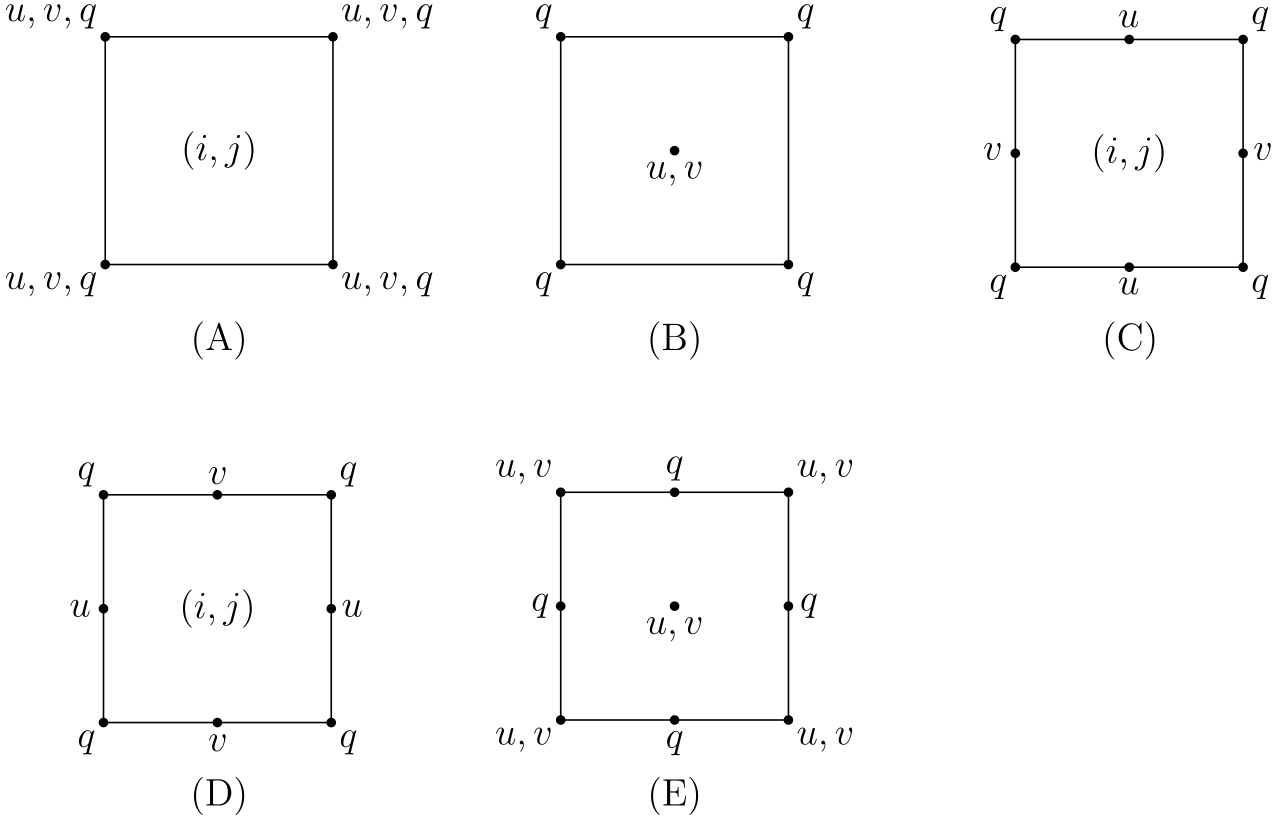
\includegraphics[width = .6\textwidth]{figs/arakawa.png}
\caption{Die fünf Gitterstrukturen nach Arakawa. Die Massenvariable wurde mit $q$ bezeichnet \cite{arakawa_grids_figure}.}
\label{fig:arakawa}
\end{figure}

Diskretisiert man ein zweidimensionales Vektorfeld auf ein ebenes Gitter, so müssen keineswegs alle Variablen an den gleichen Punkten ausgewertet werden. Die unterschiedlichen Größen können an unterschiedlichen Stellen der Polygone definiert werden. Fünf Arten, dies zu tun, sind die Arakawa-Gitter \cite{ARAKAWA1977173}, die in Abb. \ref{fig:arakawa} dargestellt sind.

Hier werden zunächst nur das A-Gitter\index{A-Gitter} und das C-Gitter\index{C-Gitter} eindimensional untersucht. Hierzu geht man vom System der linearisierten Flachwassergleichungen\index{linearisierte Flachwassergleichungen}\index{Flachwassergleichungen!linearisierte} Glg.en \eqref{eq:flach_lin_1} - \eqref{eq:flach_lin_2} ohne Corioliskraft aus:
%
\begin{align}
\frac{\partial h}{\partial t} & = -H\frac{\partial u}{\partial x}\label{eq:arakawa_deriv_0}\\
\frac{\partial u}{\partial t} & = -g\frac{\partial h}{\partial x}\label{eq:arakawa_deriv_1}
\end{align}
%
Als Ansatz macht man hier
%
\begin{align}
h = \newhat{h}\exp\left(ikx - i\omega t\right) && u = \newhat{u}\exp\left(ikx - i\omega t\right)
\end{align}
%
mit $\newhat{h}, \newhat{u} \in \mathbb{C}$. Dies führt auf
%
\begin{align}
-i\omega\newhat{h} = -Hik\newhat{u} \Leftrightarrow \omega\newhat{h} - Hk\newhat{u} = 0, && -i\omega\newhat{u} = -gik\newhat{h} \Leftrightarrow \omega\newhat{u} - gk\newhat{h} = 0. 
\end{align}
%
In Matrixschreibweise wird dies zu
%
\begin{align}
\left(\begin{array}{cc}
\omega & -Hk\\
-gk & \omega
\end{array}\right)\left(\begin{array}{c}\newhat{h}\\
\newhat{u}\end{array}\right) = \left(\begin{array}{c}
0\\
0\end{array}\right)
\end{align}
%
Nichttriviale Lösungen existieren, falls die Determinante der Matrix verschwindet:
%
\begin{align}
	\omega^2 - gHk^2 = 0 \Rightarrow \omega = k\sqrt{gH}
\end{align}
%
Hieraus folgt für die Geschwindigkeiten
%
\begin{align}
c_\text{ph} = \frac{\omega}{k} = \sqrt{gH}, && c_\text{gr} = \frac{\partial\omega}{\partial k} = \sqrt{gH} = c_\text{ph}.
\end{align}
%
Dies ist bereits die aus Glg. \eqref{eq:disp_rel_shallow_waves} bekannte Dispersionsrelation der Flachwasserwellen\index{Dispersionsrelation!Flachwasserwellen}\index{Flachwasserwelle!Dispersionsrelation}.

In der nun folgenden Herleitung der numerischen Versionen dieser Gleichungen wird von zeitlich kontinuierlichen und räumlich diskretisierten Gleichungen ausgegangen, um die Resultate nicht durch ein gewähltes Zeitschrittverfahren zu beeinflussen.

\subsection{A-Gitter}
\label{sec:a-gitter}\index{A-Gitter}

Beim A-Gitter\index{A-Gitter} werden die Oberflächenauslenkung $h$ und die Windgeschwindigkeit $u$ an denselben Orten $j\Delta x$ mit $j\in\mathbb{N}$ definiert. Man notiert hier als Ansatz
%
\begin{align}
h_j = \newhat{h}\exp\left(ikj\Delta x - i\omega t\right), && u_j = \newhat{u}\exp\left(ikj\Delta x - i\omega t\right).
\end{align}
%
Die Gleichungen \eqref{eq:arakawa_deriv_0} - \eqref{eq:arakawa_deriv_1} diskretisiert man wie folgt:
%
\begin{align}
\frac{\partial h_j}{\partial t} = -H\frac{u_{j + 1} - u_{j - 1}}{2\Delta x} && \frac{\partial u_j}{\partial t} = -g\frac{h_{j + 1} - h_{j - 1}}{2\Delta x}
\end{align}
%
Setzt man hier den Ansatz ein, erhält man
%
\begin{align}
-i\omega\newhat{h} & = -\frac{H\newhat{u}}{2\Delta x}\left[\exp\left(ik\Delta x\right) - \exp\left(-ik\Delta x\right)\right]\nonumber\\
\Leftrightarrow -i\omega\newhat{h} & = -\frac{H\newhat{u}}{2\Delta x}\left[i\sin\left(k\Delta x\right) + i\sin\left(k\Delta x\right)\right]\nonumber\\
\Leftrightarrow -i\omega\newhat{h} & = -\frac{H\newhat{u}i}{\Delta x}\sin\left(k\Delta x\right)\nonumber\\
\Leftrightarrow \omega\newhat{h} - \frac{H\newhat{u}}{\Delta x}\sin\left(k\Delta x\right) & = 0\label{eq:arakawa_deriv_2}
\end{align}
%
sowie
%
\begin{align}
-i\omega\newhat{u} & = -\frac{g\newhat{h}}{2\Delta x}\left[\exp\left(ik\Delta x\right) - \exp\left(-ik\Delta x\right)\right]\nonumber\\
\Leftrightarrow -i\omega\newhat{u} & = -\frac{g\newhat{h}}{2\Delta x}2i\sin\left(k\Delta x\right) = -\frac{g\newhat{h}}{\Delta x}i\sin\left(k\Delta x\right)\nonumber\\
\Leftrightarrow \omega\newhat{u} - \frac{g\newhat{h}}{\Delta x}\sin\left(k\Delta x\right) & = 0.\label{eq:arakawa_deriv_3}
\end{align}
%
Notiert man Glg.en \eqref{eq:arakawa_deriv_2} - \eqref{eq:arakawa_deriv_3} in Matrixschreibweise, erhält man
%
\begin{align}
\left(\begin{array}{cc}
\omega & -\frac{H}{\Delta x}\sin\left(k\Delta x\right)\\
-\frac{g}{\Delta x}\sin\left(k\Delta x\right) & \omega
\end{array}\right)\left(\begin{array}{c}\newhat{h}\\
\newhat{u}\end{array}\right) = \left(\begin{array}{c}
0\\
0\end{array}\right).
\end{align}
%
Nichttriviale Lösungen existieren, falls die Determinante der Matrix verschwindet, also für
%
\begin{align}
\omega^2 - gH\frac{\sin^2\left(k\Delta x\right)}{\left(\Delta x\right)^2} = 0, && \Rightarrow\omega = \sqrt{gH}\frac{\sin\left(k\Delta x\right)}{\Delta x}.
\end{align}
%
Hieraus folgt für die Phasengeschwindigkeit\index{Phasengeschwindigkeit!A-Gitter}\index{A-Gitter!Phasengeschwindigkeit}
%
\begin{align}
c_\text{ph} = c_\text{ph}^{\text{(real)}}\frac{\sin\left(k\Delta x\right)}{k\Delta x}\label{eq:arakawa_deriv_6}
\end{align}
%
und für die Gruppengeschwindigkeit\index{Gruppengeschwindigkeit!A-Gitter}\index{A-Gitter!Gruppengeschwindigkeit}
%
\begin{align}
c_\text{gr} = \frac{\partial\omega}{\partial k} = c_\text{gr}^{\text{(real)}}\cos\left(k\Delta x\right).\label{eq:arakawa_deriv_7}
\end{align}
%
Führt man die dimensionslose Geschwindigkeit
%
\begin{center}
\doublebox{\parbox{0.8\textwidth}{
\begin{center}
\begin{align}
\newtilde{c} \coloneqq \frac{c}{\sqrt{gH}}\label{eq:arakawa_deriv_8}
\end{align}
\end{center}
}}
\end{center}
%
sowie die dimensionslose Wellenzahl
%
\begin{center}
\doublebox{\parbox{0.8\textwidth}{
\begin{center}
\begin{align}
\kappa \coloneqq k\Delta x\label{eq:arakawa_deriv_9}
\end{align}
\end{center}
}}
\end{center}
%
ein, so lassen sich die Glg.en \eqref{eq:arakawa_deriv_6} - \eqref{eq:arakawa_deriv_7} in der Form
%
\begin{center}
\doublebox{\parbox{0.8\textwidth}{
\begin{center}
\begin{align}
\newtilde{c}_\text{ph} & = \frac{\sin\left(\kappa\right)}{\kappa},\label{eq:arakawa_deriv_10}\\
\newtilde{c}_\text{gr} & = \cos\left(\kappa\right)\label{eq:arakawa_deriv_11}
\end{align}
\end{center}
}}
\end{center}
%
notieren.

\subsection{C-Gitter}
\label{sec:c-gitter}\index{C-Gitter}

Beim C-Gitter\index{C-Gitter} werden die Windgeschwindigkeit $u$ an Orten $j\Delta x$ und die Oberflächenauslenkung $h$ and Orten $\left(j + \frac{1}{2}\right)\Delta x$ mit $j\in\mathbb{N}$ definiert. Man notiert hier als Ansatz
%
\begin{align}
h_{j + \frac{1}{2}} = \newhat{h}\exp\left(ikj\Delta x - i\omega t\right)\exp\left(\frac{ik\Delta x}{2}\right), && u_j = \newhat{u}\exp\left(ikj\Delta x - i\omega t\right).
\end{align}
%
Die Gleichungen \eqref{eq:arakawa_deriv_0} - \eqref{eq:arakawa_deriv_1} diskretisiert man wie folgt:
%
\begin{align}
\frac{\partial h_{j + \frac{1}{2}}}{\partial t} = -H\frac{u_{j + 1} - u_{j}}{2\Delta x}, && \frac{\partial u_j}{\partial t} = -g\frac{h_{j + \frac{1}{2}} - h_{j - \frac{1}{2}}}{2\Delta x}
\end{align}
%
Setzt man hier den Ansatz ein, erhält man
%
\begin{align}
-i\omega\newhat{h}\exp\left(\frac{ik\Delta x}{2}\right) & = -\frac{H\newhat{u}}{\Delta x}\left[\exp\left(ik\Delta x\right) - 1\right]\nonumber\\
\Leftrightarrow i\omega\newhat{h}\exp\left(\frac{ik\Delta x}{2}\right) - \frac{H\newhat{u}}{\Delta x}\left[\exp\left(ik\Delta x\right) - 1\right] & = 0\label{eq:arakawa_deriv_4}
\end{align}
%
sowie
%
\begin{align}
	-i\omega\newhat{u} & = -\frac{g\newhat{h}}{\Delta x}\exp\left(\frac{ik\Delta x}{2}\right)\left[1 - \exp\left(-ik\Delta x\right)\right]\nonumber\\
	\Leftrightarrow i\omega\newhat{u} - \frac{g\newhat{h}}{\Delta x}\exp\left(\frac{ik\Delta x}{2}\right)\left[1 - \exp\left(-ik\Delta x\right)\right] & = 0.\label{eq:arakawa_deriv_5}
\end{align}
%
Notiert man Glg.en \eqref{eq:arakawa_deriv_4} - \eqref{eq:arakawa_deriv_5} in Matrixschreibweise, erhält man
%
\begin{align}
\left(\begin{array}{cc}
i\omega\exp\left(\frac{ik\Delta x}{2}\right) & -\frac{H}{\Delta x}\left[\exp\left(ik\Delta x\right) - 1\right]\\
-\frac{g}{\Delta x}\left[1 - \exp\left(-ik\Delta x\right)\right] & i\omega
\end{array}\right)\left(\begin{array}{c}\newhat{h}\\
\newhat{u}\end{array}\right) = \left(\begin{array}{c}
0\\
0\end{array}\right).
\end{align}
%
Nichttriviale Lösungen existieren, falls die Determinante der Matrix verschwindet, also für
%
\begin{align}
-\omega^2 - gH\frac{\left[\exp\left(ik\Delta x\right) - 1\right]\left[1 - \exp\left(-ik\Delta x\right)\right]}{\left(\Delta x\right)^2} & = 0\nonumber\\
\Rightarrow \omega^2 & = gH\frac{\left[1 - \exp\left(ik\Delta x\right)\right]\left[1 - \exp\left(-ik\Delta x\right)\right]}{\left(\Delta x\right)^2}\nonumber\\
\Rightarrow \omega^2 & = gH\frac{2 - 2\cos\left(k\Delta x\right)}{\left(\Delta x\right)^2} = gH2\frac{1 - \cos\left(k\Delta x\right)}{\left(\Delta x\right)^2}.
\end{align}
%
Hieraus folgt für die Phasengeschwindigkeit\index{Phasengeschwindigkeit!C-Gitter}\index{C-Gitter!Phasengeschwindigkeit}
%
\begin{align}
c_\text{ph} = c_\text{ph}^{\text{(real)}}\sqrt{2\frac{1 - \cos\left(k\Delta x\right)}{\left(k\Delta x\right)^2}}\label{eq:arakawa_deriv_12}
\end{align}
%
und für die Gruppengeschwindigkeit\index{Gruppengeschwindigkeit!C-Gitter}\index{C-Gitter!Gruppengeschwindigkeit}
%
\begin{align}
c_\text{gr} = \frac{\partial\omega}{\partial k} = \frac{1}{2\omega}\frac{\partial\omega^2}{\partial k} = gH2\frac{\sin\left(k\Delta x\right)}{2\omega\Delta x} = gH\frac{\sin\left(k\Delta x\right)}{\omega\Delta x} = c_\text{gr}^{\text{(real)}}\frac{\sin\left(k\Delta x\right)}{\sqrt{2 - 2\cos\left(k\Delta x\right)}}.\label{eq:arakawa_deriv_13}
\end{align}
%
In Termen der dimensionslosen Größen Glg.en \eqref{eq:arakawa_deriv_8} - \eqref{eq:arakawa_deriv_9} kann man die Glg.en \eqref{eq:arakawa_deriv_12} - \eqref{eq:arakawa_deriv_13} in der Form
%
\begin{center}
\doublebox{\parbox{0.8\textwidth}{
\begin{center}
\begin{align}
\newtilde{c}_\text{ph} = \sqrt{2\frac{1 - \cos\left(\kappa\right)}{\left(\kappa\right)^2}}, && \newtilde{c}_\text{gr} = \frac{\sin\left(\kappa\right)}{\sqrt{2 - 2\cos\left(\kappa\right)}}
\end{align}
\end{center}
}}
\end{center}
%
notieren. Abb. \ref{fig:arakawa_disp_relations} zeigt die Dispersionsrelationen des A-Gitters\index{Dispersionsrelation!A-Gitter}\index{A-Gitter!Dispersionsrelation} sowie des C-Gitters\index{Dispersionsrelation!C-Gitter}\index{C-Gitter!Dispersionsrelation}.

\begin{figure}
\centering
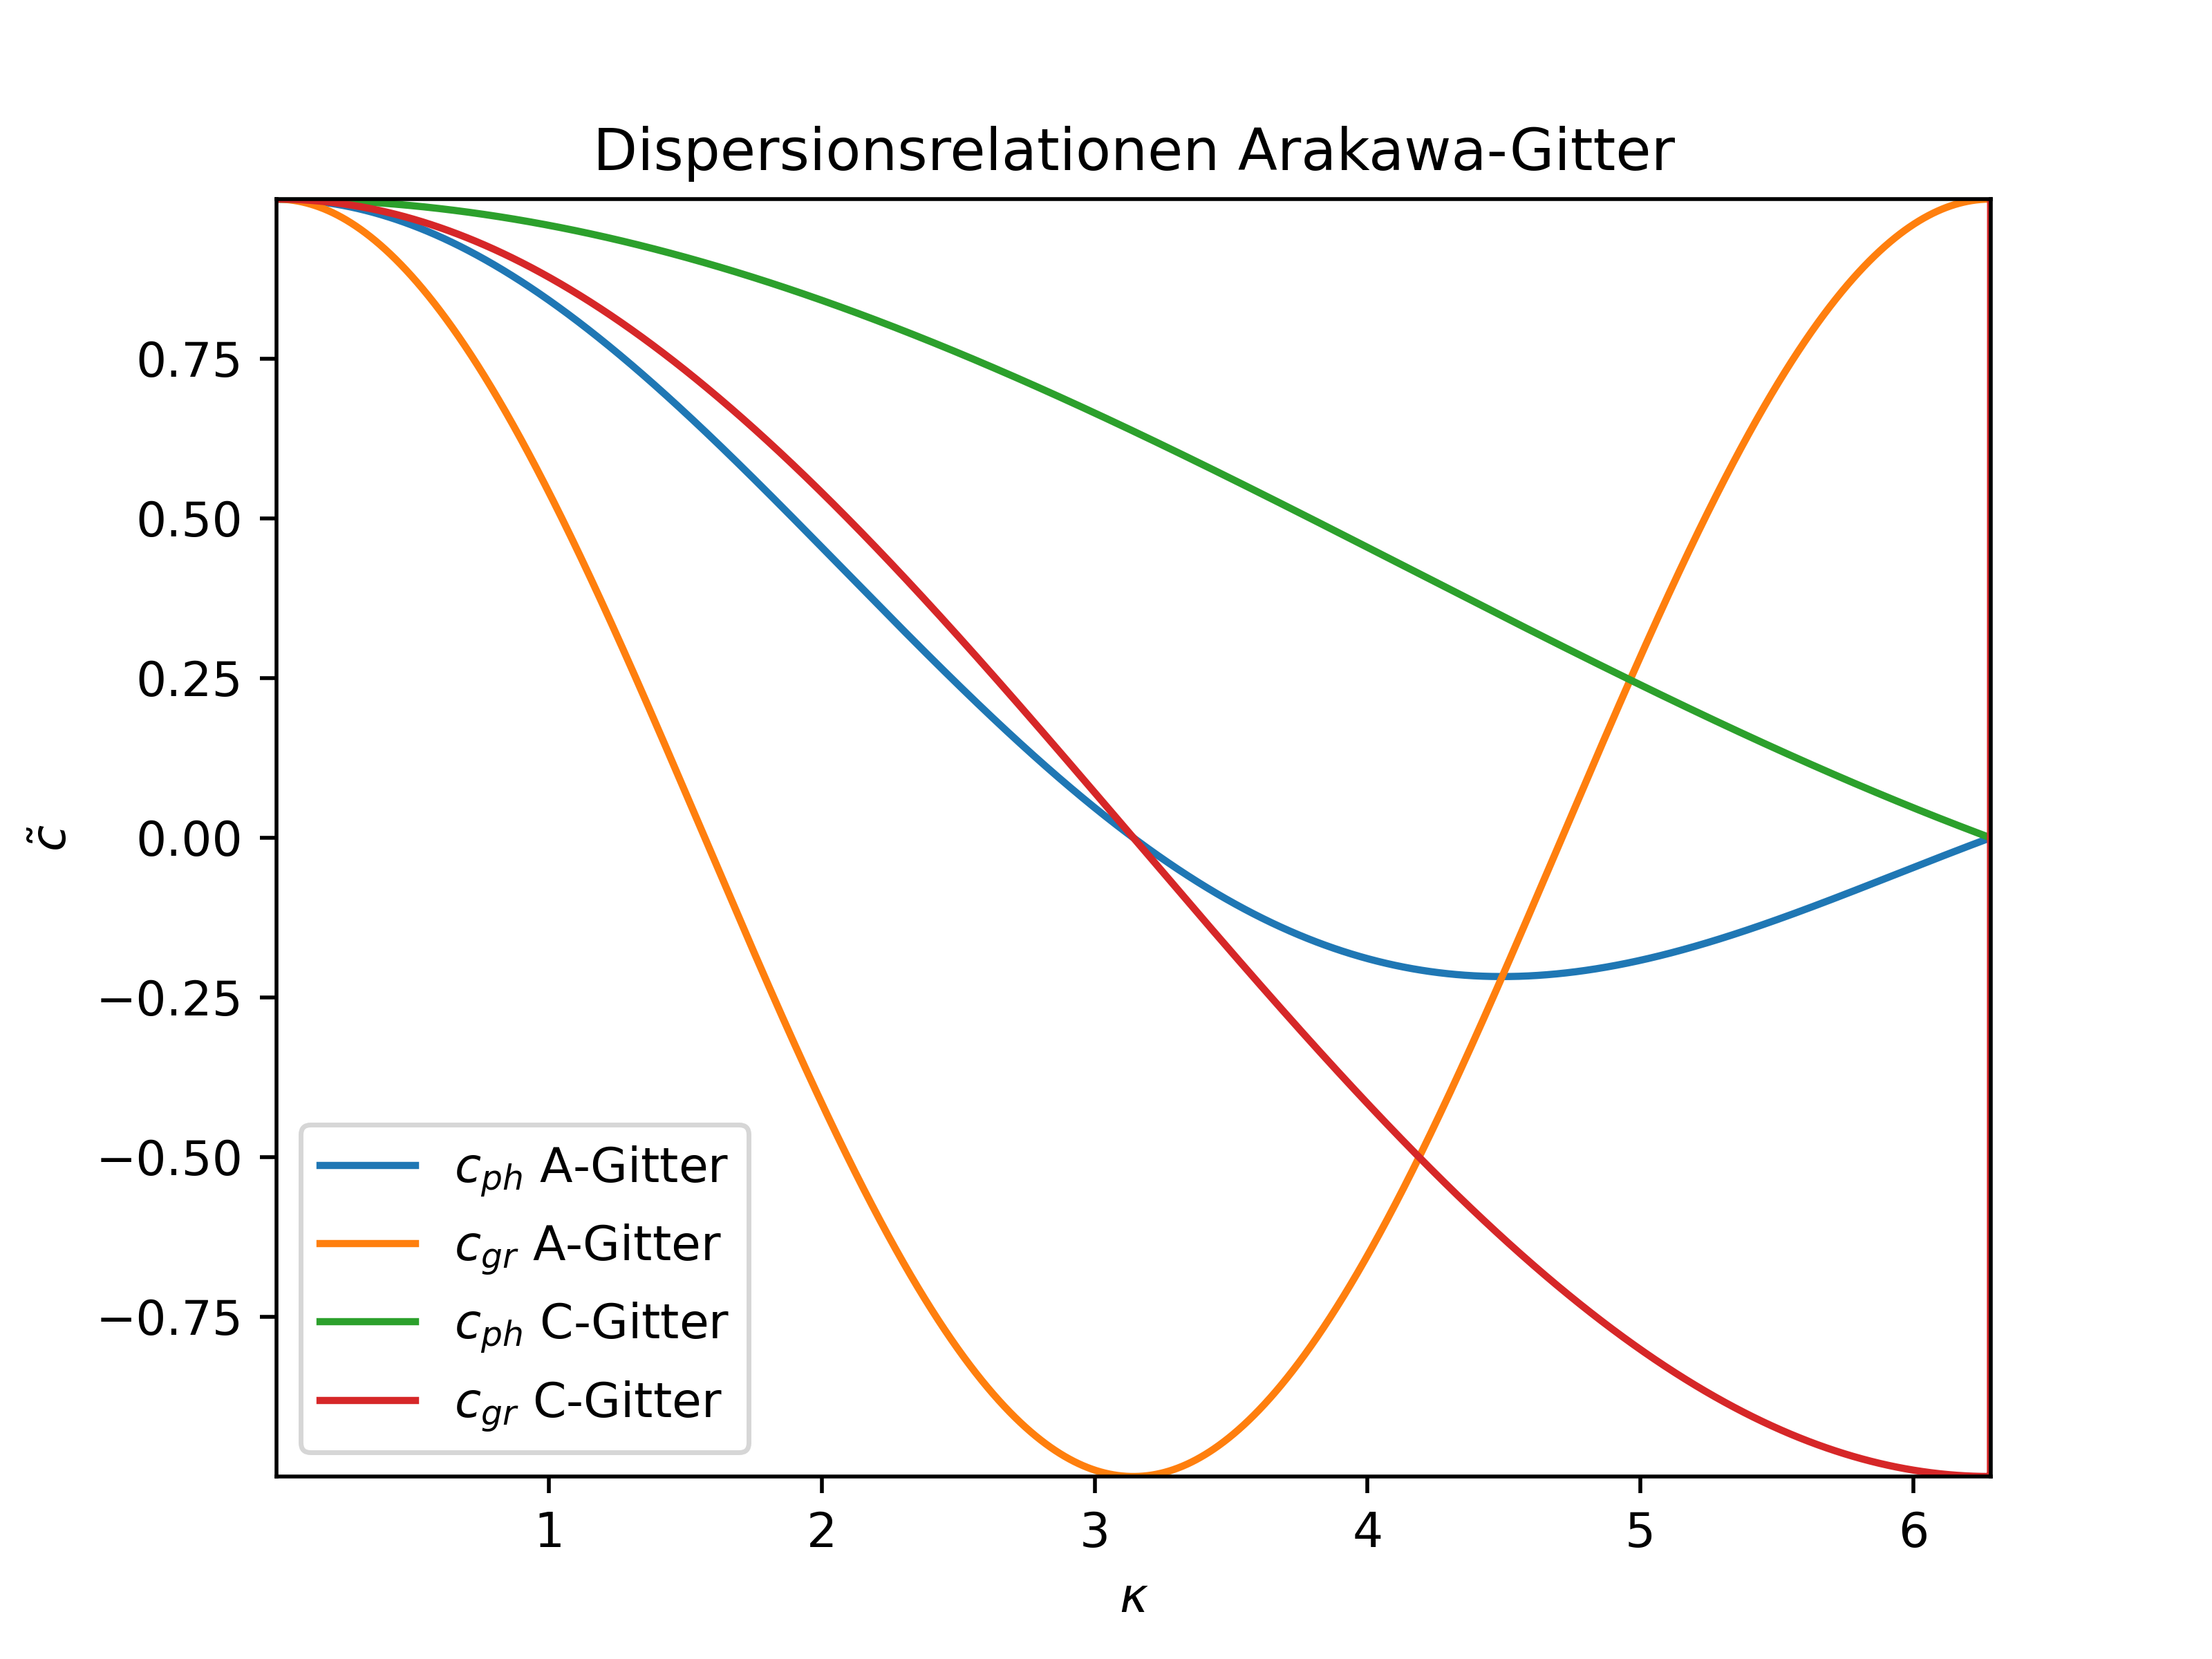
\includegraphics[width = .7\textwidth]{figs/arakawa_disp_relations.png}
\caption{Die Dispersionsrelationen des A-Gitters und des C-Gitters.}
\label{fig:arakawa_disp_relations}
\end{figure}

\section{Skalare Erhaltungseigenschaften auf dem C-Gitter}
\label{sec:skalare_erhaltungseigenschaften_auf_dem_c-gitter}

Ist $q$ eine Erhaltungsgröße, also eine Größe, für die $\md{q} = 0$ gilt, so kann man für $\newtilde{q} \coloneqq \rho q$ eine Kontinuitätsgleichung herleiten:
%
\begin{align}
\md{q} = \frac{\partial q}{\partial t} + \mathbf{v}\cdot\nabla q & = 0,\\
\frac{\partial\rho}{\partial t} + \mathbf{v}\cdot\nabla \rho + \rho\nabla\cdot\mathbf{v} & = 0,\\
\Rightarrow \frac{\partial\newtilde{q}}{\partial t} + \nabla\cdot \mathbf{j}_{\newtilde{q}} & = 0,
\end{align}
%
wobei die Größe $\mathbf{j}_{\newtilde{q}} \coloneqq \newtilde{q}\mathbf{v}$ den Fluss der Größe $q$ bezeichnet. Definiert man
%
\begin{align}
Q \coloneqq \int_A\newtilde{q}d^3r
\end{align}
%
als das globale Integral der Größe $q$, so ist $Q$ unter kinematischen Randbedingungen erhalten:
%
\begin{align}
\frac{dQ}{dt} = -\int_A\nabla\cdot \mathbf{j}_{\newtilde{q}}d^3r = -\int_{\partial A}\mathbf{j}_{\newtilde{q}}\cdot d\mathbf{n}
\end{align}
%
Zerlegt man $A$ nun in $N \geq 1$ Gitterboxen $A = A_1 \cup A_2 \cup \dots \cup A_N$, so gilt
%
\begin{align}
Q = \sum_{i = 1}^NQ_i
\end{align} 
%
mit
%
\begin{align}
Q_i\coloneqq\int_{A_i}\newtilde{q}d^3r.
\end{align}
%
Somit gilt
%
\begin{align}
\frac{dQ}{dt} = \sum_{i = 1}^N\frac{dQ_i}{dt} = -\sum_{i = 1}^N\int_{\partial A_i}\mathbf{j}_{\newtilde{q}}\cdot d\mathbf{n} = -\sum_{i = 1}^N\sum_{F \in F_i}\mathbf{j}_{\newtilde{q}}\cdot\mathbf{n}_F,
\end{align}
%
wobei $F_i$ die Menge aller Seitenflächen der Gitterbox $i$ ist, und $\mathbf{n}_F$ der auf der Fläche $F$ senkrecht stehende Normalenvektor (nach außen zeigend). Dabei wird davon ausgegangen, dass $\partial A_i$ jeweils aus einer Anzahl glatter Flächen besteht, über die einzeln zu summieren ist, da sie durch Kanten getrennt sind. Da jede Fläche $F$ in der Doppelsumme zweimal auftritt, jedoch der Vektor $\mathbf{n}$ dabei in zwei entgegengesetzte Richtungen zeigt, ergibt sich die Summe zu Null, sodass auf einem C-Gitter auch nach der Diskretisierung
%
\begin{center}
\doublebox{\parbox{0.8\textwidth}{
\begin{center}
\begin{align}
Q = \text{const.}
\end{align}
\end{center}
}}
\end{center}
%
gilt. Flächen, die Teil von $\partial A$ sind, stellen dabei trivialerweise kein Problem da, da durch sie unter kinematischen Randbedingungen per Definition überhaupt kein Massenfluss stattfindet. Auch unter der verallgemeinerten Voraussetzung, dass $\mathbf{j}_{\newtilde{q}}$ nicht nur aus $\newtilde{q}\mathbf{v}$, sondern aus weiteren, insbesondere diffusiven Flüssen besteht, gilt dies noch. Angemerkt werden sollte außerdem, dass selbst bei fehlerhafter Berechnung von Gittergeometrien $Q$ eine Erhaltungsgröße bleibt.

\section{Gradientenfelder auf dem C-Gitter}
\label{sec:gradientenfelder_auf_dem_c-gitter}\index{Gradientenfeld!C-Gitter}\index{C-Gitter!Gradientenfeld}

Seien $\psi$ ein Skalarfeld $\nabla\psi$ der Gradient dieses Skalarfeldes, dies ist ein Vektorfeld. Auf dem C-Gitter wird die Rotation eines Vektorfeldes $\mathbf{v}$ durch Anwendung des Stokes'schen Satzes auf ein Polygon mit Fläche $A$ und Kantenlängen $l_i$ ermittelt. Es gilt also
%
\begin{align}
\mathbf{k}\cdot\nabla\times\mathbf{v} = \frac{1}{A}\sum_{i}\gamma_il_iv_i,
\end{align}
%
wobei $v_i$ der Wert von $\mathbf{v}$ an der Kante $i$ ist und $\gamma_i = 1$ ist, falls der Einheitsvektor der Kante in mathmetisch positiver Zirkulationsrichtung um das Polygon zeigt, andernfalls ist $\gamma_i = -1$. Der Einfachheit halber nimmt man o. B. d. A. an, dass $\gamma_i = 1$ für alle $i$ ist, sodass man
%
\begin{align}
\mathbf{k}\cdot\nabla\times\mathbf{v} = \frac{1}{A}\sum_{i}l_iv_i
\end{align}
%
notieren kann. Nun setzt man
%
\begin{align}
\mathbf{v} = \nabla\psi
\end{align}
%
an, was auf
%
\begin{align}
\mathbf{k}\cdot\nabla\times\mathbf{v} = \frac{1}{A}\sum_{i}l_i\left(\nabla\psi\right)_i\label{eq:c-grid_rot_kons_deriv_0}
\end{align}
%
führt. Es gilt
%
\begin{align}
\left(\nabla\psi\right)_i = \frac{\psi_{\text{to}\left(i\right)} - \psi_{\text{from}\left(i\right)}}{l_i}.
\end{align}
%
Setzt man dies in Glg. \eqref{eq:c-grid_rot_kons_deriv_0} ein, erhält man
%
\begin{align}
\mathbf{k}\cdot\nabla\times\psi = \frac{1}{A}\sum_{i}l_i\frac{\psi_{\text{to}\left(i\right)} - \psi_{\text{from}\left(i\right)}}{l_i} = \frac{1}{A}\sum_{i}\psi_{\text{to}\left(i\right)} - \psi_{\text{from}\left(i\right)}.\label{eq:c-grid_rot_kons_deriv_1}
\end{align}
%
Sortiert man die Kanten in mathematisch positiver Zirkulationsrichtung um das betrachtete Polygon, gilt
%
\begin{align}
\psi_{\text{to}\left(i\right)} = \psi_{\text{from}\left(i + 1\right)}.
\end{align}
%
Jeder Wert von $\psi$ tritt in Glg. \eqref{eq:c-grid_rot_kons_deriv_1} also zweimal auf, einmal mit positivem und einmal mit negativem Vorzeichen. Dies gilt unabhängig von der betrachteten Raumrichtung. Somit gilt auf einem C-Gitter
%
\begin{center}
\doublebox{\parbox{0.8\textwidth}{
\begin{center}
\begin{align}
\nabla\times\nabla\psi = \mathbf{0}.
\end{align}
\end{center}
}}
\end{center}

\section{Skalarprodukt auf dem C-Gitter}
\label{sec:skalarprodukt_auf_dem_c-gitter}\index{Skalarprodukt!C-Gitter}\index{C-Gitter!Skalarprodukt}

Zunächst wird in diesem Abschnitt von einem rechteckigen C-Gitter ausgegangen. Während auf solch einem Gitter die Diskretisierungen von Gradient und Divergenz eindeutig sind, ist dies beim Skalarprodukt\index{Skalarprodukt!C-Gitter}\index{C-Gitter!Skalarprodukt} nicht der Fall. Als Forderung an die Diskretisierung des Skalarproduktes\index{Diskretisierung!Skalarprodukt}\index{Skalarprodukt!Diskretisierung} verwendet man, dass die Identität
%
\begin{align}
\nabla\cdot\left(\psi\mathbf{v}\right) = \mathbf{v}\cdot\nabla\psi + \psi\nabla\cdot\mathbf{v}
\end{align}
%
sich auf die Diskretisierung übertragen soll.

\subsection{Eindimensionaler Fall}
\label{sec:eindimensionaler_fall}

Die Notation wird aus Absch. \ref{sec:c-gitter} mit der Ersetzung $h \to \psi$ übernommen.
%
\begin{align}
\nabla\cdot\left(\psi u\right) &= \frac{\newtilde{\psi}_{j + 1}u_{j + 1} - \newtilde{\psi}_{j}u_{j}}{\Delta x} = \frac{\left(\psi_{j + 3/2} + \psi_{j + 1/2}\right)u_{j + 1} - \left(\psi_{j + 1/2} + \psi_{j - 1/2}\right)u_{j}}{2\Delta x}\nonumber\\
&= \frac{\psi_{j + 3/2}u_{j + 1} - \psi_{j - 1/2}u_{j} + \psi_{j + 1/2}\left(u_{j + 1} - u_{j}\right)}{2\Delta x}\nonumber\\
&= \frac{\psi_{j + 3/2}u_{j + 1} - \psi_{j - 1/2}u_{j} - \psi_{j + 1/2}\left(u_{j + 1} - u_{j}\right) + 2\psi_{j + 1/2}\left(u_{j + 1} - u_{j}\right)}{2\Delta x}\nonumber\\
&= \frac{\left(\psi_{j + 3/2} - \psi_{j + 1/2}\right)u_{j + 1} - \left(\psi_{j - 1/2} - \psi_{j + 1/2}\right)u_{j} + 2\psi_{j + 1/2}\left(u_{j + 1} - u_{j}\right)}{2\Delta x}\nonumber\\
&= \frac{1}{2}\left[\frac{\psi_{j + 3/2} - \psi_{j + 1/2}}{\Delta x}u_{j + 1} + \frac{\psi_{j + 1/2} - \psi_{j - 1/2}}{\Delta x}u_{j}\right]+ \psi_{j + 1/2}\frac{u_{j + 1} - u_{j}}{\Delta x}\nonumber\\
&\stackrel{!}{=} \psi\nabla\cdot\left(u\right) + u\frac{\partial\psi}{\partial x}
\end{align}
%
Die Produktregel überträgt sich also, falls man das Skalarprodukt $uv$ zweier Vektorfelder $u$, $v$ durch
%
\begin{align}
\left(uv\right)_{j + 1/2} = \frac{u_jv_j + u_{j + 1}v_{j + 1}}{2}
\end{align}
%
definiert.

\subsection{Dreidimensionaler rechteckiger Fall}
\label{sec:dreidimensionaler_rechteckiger_fall}

Summiert man die Herleitung im vorherigen Abschnitt über alle drei Raumrichtungen, erhält man die analoge Aussage für den dreidimensionalen Fall mit einem Skalarprodukt
%
\begin{align}
\mathbf{u}\cdot\mathbf{v} = \sum_{e\in c}\frac{u_ev_e}{2},
\end{align}
%
wobei $c$ die Menge aller Seitenflächen $e$ der betrachteten Box ist.

\subsection{Zweidimensionales orthogonales Gitter}
\label{sec:zweidimensionales_orthogonales_gitter}

Sei $A_c$ der Flächeninhalt der Zelle $c$, $e$ eine Kante der Zelle, $o\left(e\right)$ die an die Kante $e$ grenzende Nachbarzelle von $c$, $d_e$ eine duale Kantenlänge und $l_e$ eine primäre Kantenlänge. Man notiert zunächst
%
\begin{align}
\nabla\cdot\left(\psi\mathbf{v}\right) &= \frac{1}{A_c}\sum_{e\in c}l_e\frac{\psi_{o(e)} + \psi_c}{2}u_e,\\
\psi\nabla\cdot\mathbf{v} &= \frac{\psi_c}{A_c}\sum_{e\in c}l_eu_e.
\end{align}
%
Man fordert nun
%
\begin{align}
\mathbf{v}\cdot\nabla\psi &\stackrel{!}{=} \nabla\cdot\left(\psi\mathbf{v}\right) - \psi\nabla\cdot\mathbf{v}\nonumber\\
\Leftrightarrow\mathbf{v}\cdot\nabla\psi &= \frac{1}{A_c}\sum_{e\in c}l_e\frac{\psi_{o(e)} + \psi_c}{2}u_e - \frac{\psi_c}{A_c}\sum_{e\in c}l_eu_e = \frac{1}{A_c}\sum_{e\in c}l_e\frac{\psi_{o(e)} - \psi_c}{2}u_e = \frac{1}{A_c}\sum_{e\in c}\frac{\psi_{o(e)} - \psi_c}{d_e}u_e\frac{l_ed_e}{2}\nonumber\\
&= \sum_{e\in c}\frac{l_ed_e}{2A_c}\frac{\psi_{o(e)} - \psi_c}{d_e}u_e.
\end{align}
%
Hieraus leitet man
%
\begin{align}
\mathbf{u}\cdot\mathbf{v} = \sum_{e\in c}\frac{l_ed_e}{2A_c}u_eu_e
\end{align}
%
als Diskretisierung für das Skalarprodukt ab. Im ebenen Fall ergibt sich für die Summe der Gewichtungsfaktoren
%
\begin{align}
\sum_{e\in c}\frac{l_ed_e}{2A_c} = 2.
\end{align}
%
Im gekrümmten Fall, wie z. B. einer Kugeloberfläche, ist dies jedoch im Allgemeinen nicht mehr der Fall.

\subsection{Dreidimensionales orthogonales Gitter (shallow)}
\label{sec:dreidimensionales_orthogonales_gitter_(shallow)}

Nun wird die Herleitung im vorherigen Abschnitt auf ein dreidimensionales Gitter verallgemeinert, dessen Schichtdickte $\Delta z_k$ nur vom vertikalen Index $k$ abhängt. Vertikale Vektorkomponenten werden mit $w$ bezeichnet, der Index $u$ bezeichnet den vektoriellen oder skalaren Gitterpunkt über der betrachteten Gitterbox, der Index $l$ den jeweiligen Gitterpunkt darunter. Dies führt auf
%
\begin{align}
\nabla\cdot\left(\psi\mathbf{v}\right) &= \frac{1}{A_c\Delta z_k}\left(\sum_{e\in c}l_e\Delta z_k\frac{\psi_{o(e)} + \psi_c}{2}u_e + A_c\frac{\psi_u + \psi_c}{2}w_u - A_c\frac{\psi_l + \psi_c}{2}w_l\right),\label{eq:div_c-grid_shallow_no_terrain}\\
\psi\nabla\cdot\mathbf{v} &= \frac{\psi_c}{A_c\Delta z_k}\left(\sum_{e\in c}l_e\Delta z_ku_e + A_cw_u - A_cw_l\right).
\end{align}
%
Man fordert nun wieder
%
\begin{align}
\mathbf{v}\cdot\nabla\psi &\stackrel{!}{=} \nabla\cdot\left(\psi\mathbf{v}\right) - \psi\nabla\cdot\mathbf{v}\nonumber\\
\Leftrightarrow\mathbf{v}\cdot\nabla\psi &= \frac{1}{A_c\Delta z_k}\left(\sum_{e\in c}l_e\Delta z_k\frac{\psi_{o(e)} + \psi_c}{2}u_e + A_c\frac{\psi_u + \psi_c}{2}w_u - A_c\frac{\psi_l + \psi_c}{2}w_l - \psi_c\sum_{e\in c}l_e\Delta z_ku_e - \psi_cA_cw_u + \psi_cA_cw_l\right)\nonumber\\
\Leftrightarrow\mathbf{v}\cdot\nabla\psi &= \frac{1}{A_c\Delta z_k}\left(\sum_{e\in c}l_e\Delta z_k\frac{\psi_{o(e)} - \psi_c}{2}u_e + A_c\frac{\psi_u - \psi_c}{2}w_u + A_c\frac{\psi_c - \psi_l}{2}w_l\right)\nonumber\\
\Leftrightarrow\mathbf{v}\cdot\nabla\psi &= \sum_{e\in c}\frac{l_ed_e}{2A_c}\frac{\psi_{o(e)} - \psi_c}{d_e}u_e + \frac{\Delta z_{k - 1/2}}{2\Delta z_k}\frac{\psi_u - \psi_c}{\Delta z_{k - 1/2}}w_u + \frac{\Delta z_{k + 1/2}}{2\Delta z_k}\frac{\psi_c - \psi_l}{\Delta z_{k + 1/2}}w_u.
\end{align}
%
Hieraus leitet man
%
\begin{center}
\doublebox{\parbox{0.8\textwidth}{
\begin{center}
\begin{align}
\mathbf{u}^{(1)}\cdot\mathbf{u}^{(2)} = \sum_{e\in c}\frac{l_ed_e}{2A_c}u_e^{(1)}u_e^{(2)} + \frac{\Delta z_{k - 1/2}}{2\Delta z_k}w_u^{(1)}w_u^{(2)} + \frac{\Delta z_{k + 1/2}}{2\Delta z_k}w_l^{(1)}w_l^{(2)}\label{eq:inner_c-grid_3d_shallow}
\end{align}
\end{center}
}}
\end{center}
%
als Diskretisierung für das Skalarprodukt ab in der shallow atmosphere. Im ebenen Fall ergibt sich für die Summe der Gewichtungsfaktoren
%
\begin{align}
\sum_{e\in c}\frac{l_ed_e}{2A_c} + \frac{\Delta z_{k - 1/2} + \Delta z_{k + 1/2}}{2\Delta z_k} = 3,
\end{align}
%
wobei
%
\begin{align}
\Delta z_k &= z_{k - 1/2} - z_{k + 1/2} = \frac{z_{k - 1} + z_k}{2} - \frac{z_{k} + z_{k + 1}}{2} = \frac{z_{k - 1} + z_k - z_{k} - z_{k + 1}}{2}\nonumber\\
&= \frac{z_{k - 1} - z_{k} + z_k - z_{k + 1}}{2} = \frac{\Delta z_{k - 1/2} + \Delta z_{k + 1/2}}{2}
\end{align}
%
eingesetzt wurde. Im gekrümmten Fall, wie z. B. einer Kugeloberfläche, ist dies jedoch im Allgemeinen nicht mehr der Fall.

\subsection{Dreidimensionales orthogonales Gitter (deep)}
\label{sec:dreidimensionales_orthogonales_gitter_(deep)}

Nun wird die Herleitung im vorherigen Abschnitt auf die deep atmosphere verallgemeinert, d. h. die shallow-Atmosphere-Approximation wird aufgehoben. Man geht wieder davon aus, dass die Schichtdickte $\Delta z_k$ nur vom vertikalen Index $k$ abhängt. Mit der gleichen Indexnotation wie im vorherigen Abschnitt erhält man
%
\begin{align}
\nabla\cdot\left(\psi\mathbf{v}\right) &= \frac{1}{V_{c, k}}\left(\sum_{e\in c}A_{e, k}\frac{\psi_{o(e)} + \psi_c}{2}u_{e, k} + A_{c, k - 1/2}\frac{\psi_{c, k} + \psi_{c, k - 1}}{2}w_{c, k - 1/2} -  A_{c, k + 1/2}\frac{\psi_{c, k - 1} + \psi_{c, k}}{2}w_{c, k + 1/2}\right),\label{eq:div_c-grid_deep_no_terrain}\\
\psi\nabla\cdot\mathbf{v} &= \frac{\psi_c}{V_{c, k}}\left(\sum_{e\in c}A_{e, k}u_{e, k} + A_{c, k - 1/2}w_{c, k - 1/2} - A_{c, k + 1/2}w_{c, k + 1/2}\right).
\end{align}
%
Die Zellen-Grundfläche $A_{c, k - 1/2}$ ist nun auch vom vertikalen Index abhängig. $A_{e, k}$ ist die vertikale Fläche, deren Teilmenge die Kante $\left(e, k\right)$ ist. Man fordert nun wieder
%
\begin{align}
\mathbf{v}\cdot\nabla\psi &\stackrel{!}{=} \nabla\cdot\left(\psi\mathbf{v}\right) - \psi\nabla\cdot\mathbf{v}\nonumber\\
\Leftrightarrow\mathbf{v}\cdot\nabla\psi &= \frac{1}{V_{c, k}}\Bigg(\sum_{e\in c}A_{e, k}\frac{\psi_{o(e), k} + \psi_{c, k}}{2}u_{e, k} + A_{c, k - 1/2}\frac{\psi_{c, k} + \psi_{c, k - 1}}{2}w_{c, k - 1/2} -  A_{c, k + 1/2}\frac{\psi_{c, k - 1} + \psi_{c, k}}{2}w_{c, k + 1/2}\nonumber\\
&- \sum_{e\in c}A_{e, k}\psi_{c, k}u_{e, k} - A_{c, k - 1/2}\psi_{c, k}w_{c, k - 1/2} + A_{c, k + 1/2}\psi_{c, k}w_{c, k + 1/2}\Bigg)\nonumber\\
\Leftrightarrow\mathbf{v}\cdot\nabla\psi &= \frac{1}{V_{c, k}}\left(\sum_{e\in c}A_{e, k}\frac{\psi_{o(e), k} - \psi_{c, k}}{2}u_{e, k} + A_{c, k - 1/2}\frac{\psi_{c, k - 1} - \psi_{c, k}}{2}w_{c, k - 1/2} + A_{c, k + 1/2}\frac{\psi_{c, k} - \psi_{c, k + 1}}{2}w_{c, k + 1/2}\right)\nonumber\\
\Leftrightarrow\mathbf{v}\cdot\nabla\psi &= \sum_{e\in c}\frac{A_{e, k}d_{e, k}}{2V_{c, k}}\frac{\psi_{o(e), k} - \psi_{c, k}}{d_{e, k}}u_{e, k} + \frac{A_{c, k - 1/2}\Delta z_{k - 1/2}}{2V_{c, k}}\frac{\psi_{c, k - 1} - \psi_{c, k}}{\Delta z_{k - 1/2}}w_{c, k - 1/2}\nonumber\\
&+ \frac{A_{c, k + 1/2}\Delta z_{k + 1/2}}{2V_{c, k}}\frac{\psi_{c, k} - \psi_{c, k + 1}}{\Delta z_{k + 1/2}}w_{c, k + 1/2}.
\end{align}
%
Hieraus leitet man
%
\begin{center}
\doublebox{\parbox{0.8\textwidth}{
\begin{center}
\begin{align}
\mathbf{u}^{(1)}\cdot\mathbf{u}^{(2)} &= \sum_{e\in c}\frac{A_{e, k}d_{e, k}}{2V_{c, k}}u_{e, k}^{(1)}u_{e, k}^{(2)} + \frac{A_{c, k - 1/2}\Delta z_{k - 1/2}}{2V_{c, k}}w_{c, k - 1/2}^{(1)}w_{c, k - 1/2}^{(2)}\nonumber\\
&+ \frac{A_{c, k + 1/2}\Delta z_{k + 1/2}}{2V_{c, k}}w_{c, k + 1/2}^{(1)}w_{c, k + 1/2}^{(2)}\label{eq:inner_c-grid_3d_deep}
\end{align}
\end{center}
}}
\end{center}
%
als Diskretisierung für das Skalarprodukt ab. Setzt man hier die Approximationen
%
\begin{align}
V_{c, k} &\approx A_{c, k}\Delta z_{k},\\
A_{e, k} &\approx l_{e, k}\Delta z_{k}
\end{align}
%
ein, erhält man unter Vernachlässigung des Ungefähr-Zeichens
%
\begin{align}
\mathbf{u}^{(1)}\cdot\mathbf{u}^{(2)} &= \sum_{e\in c}\frac{l_{e, k}d_{e, k}}{2A_{c, k}}u_{e, k}^{(1)}u_{e, k}^{(2)} + \frac{A_{c, k - 1/2}\Delta z_{k - 1/2}}{2A_{c, k}\Delta z_{k}}w_{c, k - 1/2}^{(1)}w_{c, k - 1/2}^{(2)} + \frac{A_{c, k + 1/2}\Delta z_{k + 1/2}}{2A_{c, k}\Delta z_{k}}w_{c, k + 1/2}^{(1)}w_{c, k + 1/2}^{(2)}.
\end{align}
%
Nun setzt man
%
\begin{align}
A_{c, k} = \left(\frac{r_k}{a}\right)^2A_c
\end{align}
%
an, wobei $a$ der mittlere Erdradius ist und $A_c$ die Grundfläche der Zelle auf Höhe des Erdradius ist. Analog setzt man für die Längen
%
\begin{align}
l_{e, k} &= \frac{r_k}{a}l_e,\\
d_{e, k} &= \frac{r_k}{a}d_e
\end{align}
%
an. Hieraus folgt
%
\begin{center}
\doublebox{\parbox{0.8\textwidth}{
\begin{center}
\begin{align}
\mathbf{u}^{(1)}\cdot\mathbf{u}^{(2)} &= \sum_{e\in c}\frac{a^2r_k^2l_{e}d_{e}}{2a^2r_k^2A_c}u_{e, k}^{(1)}u_{e, k}^{(2)} + \frac{r_{k - 1/2}^2A_c\Delta z_{k - 1/2}}{2r_k^2A_c\Delta z_{k}}w_{c, k - 1/2}^{(1)}w_{c, k - 1/2}^{(2)} + \frac{r_{k + 1/2}^2A_c\Delta z_{k + 1/2}}{2r_k^2A_c\Delta z_{k}}w_{c, k + 1/2}^{(1)}w_{c, k + 1/2}^{(2)}\nonumber\\
&= \sum_{e\in c}\frac{l_{e}d_{e}}{2A_c}u_{e, k}^{(1)}u_{e, k}^{(2)} + \frac{r_{k - 1/2}^2\Delta z_{k - 1/2}}{2r_k^2\Delta z_{k}}w_{c, k - 1/2}^{(1)}w_{c, k - 1/2}^{(2)} + \frac{r_{k + 1/2}^2\Delta z_{k + 1/2}}{2r_k^2\Delta z_{k}}w_{c, k + 1/2}^{(1)}w_{c, k + 1/2}^{(2)}
\end{align}
\end{center}
}}
\end{center}
%
In der shallow atmosphere nimmt man $r_k = r_{k - 1/2} = a$ und Höhenunabhängigkeit aller Gittereigenschaften an, dies führt auf Glg. \eqref{eq:inner_c-grid_3d_shallow}:
%
\begin{align}
\mathbf{u}^{(1)}\cdot\mathbf{u}^{(2)}\vline_\text{shallow} &= \sum_{e\in c}\frac{l_ed_e}{2A_c}u_{e, k}^{(1)}u_{e, k}^{(2)} + \frac{\Delta z_{k - 1/2}}{2\Delta z_{k}}w_{c, k - 1/2}^{(1)}w_{c, k - 1/2}^{(2)} + \frac{\Delta z_{k + 1/2}}{2\Delta z_{k}}w_{c, k + 1/2}^{(1)}w_{c, k + 1/2}^{(2)}
\end{align}

\section{Festlegung auf das C-Gitter}
\label{sec:festlegung_auf_das_c-gitter}\index{C-Gitter}

Das C-Gitter\index{C-Gitter} hat gegenüber den anderen Gittern zusammenfassend drei Vorteile:
%
\begin{enumerate}
\item Es hat vorteilhafte Dispersionsrelationen\index{Dispersionsrelation}.
\item Erhaltung skalarer Variablen ist leicht zu gewährleisten.
\item Gradientenfelder sind rotationsfrei.
\item Die Produktregel\index{Produktregel!C-Gitter}\index{C-Gitter!Produktregel} $\nabla\cdot\left(\psi\mathbf{v}\right) = \mathbf{v}\cdot\nabla\psi + \psi\nabla\cdot\mathbf{v}$ reproduziert sich bei passender Diskretisierung des Skalarproduktes.
\end{enumerate}
%
Daher wird an dieser Stelle die Entscheidung getroffen, ein C-Gitter\index{C-Gitter} für den in Teil \ref{part:entwicklung_eines_dynamischen_kerns} zu entwickelnden dynamischen Kern\index{dynamischer Kern}\index{Kern!dynamischer}.

\subsection{Folgerungen}
\label{sec:folgerungen_c-gitter}\index{C-Gitter}

Die Vektoren befinden sich bei einem C-Gitter\index{C-Gitter} auf den Kanten und schneiden diese orthogonal. Verlängert man die Vektorpfeile in beide Richtungen, landet man an den skalaren Datenpunkten. Das so erhaltene Gitter ist das sogenannte \textit{duale Gitter}\index{duales Gitter}\index{Gitter!duales}. Gitter, die ein duales Gitter haben, bezeichnet man als \textit{orthogonal}\index{orthogonales Gitter}\index{Gitter!orthogonales}. Dies ist nicht immer der Fall. Um die positiven Eigenschaften des C-Gitters\index{C-Gitter} nutzen zu können, legt man sich an dieser Stelle auf ein orthogonales Gitter\index{orthogonales Gitter}\index{Gitter!orthogonales} für den in Teil \ref{part:entwicklung_eines_dynamischen_kerns} zu formulierenden dynamischen Kern\index{dynamische Kern}\index{Kern!dynamischer} fest.

\section{Das Problem des Verhältnisses der Freiheitsgrade}
\label{sec:das_problem_des_verhältnisses_der_freiheitsgrade}

Im kontinuierlichen Fall gelten für $N \geq 1$ prognostische Variablen\index{prognostische Variable}\index{Variable!prognostische} $\psi_i$ mit $1 \leq i \leq N$ ein System aus $N$ prognostischen Gleichungen\index{prognostische Gleichung}\index{Gleichung!prognostische}. Linearisiert man diese, entsteht ein lineares gekoppeltes partielles Differenzialgleichungssystem. Nimmt man keine externen Forcings auf, ist dieses homogen. Setzt man für jede der prognostischen Variablen eine ebene Welle $\psi_i = \newhat{\psi}_i\exp\left(i\mathbf{k}\cdot\mathbf{r} - i\omega t\right)$ mit $\newhat{\psi}_i\in\mathbb{C}$ ein, entsteht homogenes lineares Gleichungssystem für die komplexen Amplituden $\newhat{\psi}_i$. Dies ist ein Eigenwertproblem für die Frequenz $\omega$. Die Eigenwerte findet man über Nullsetzen des charakteristischen Polynoms (der Determinante) dieses Gleichungssystems. Das charakteristische Polynom hat nach dem Hauptsatz der Algebra\index{Hauptsatz der Algebra}\index{Algebra!Hauptsatz der} $N$ komplexe, allerdings nicht notwendigerweise verschiedene Nullstellen. Jede der verschiedenen Nullstellen entspricht einem Zweig der Dispersionsrelation.

Bei der Diskretisierung ist dies insbesondere beim Staggering von Vektorfeldern wichtig. Im Falle der linearisierten shallow water equations hat man drei Gleichungen für die drei Variablen $\left(u, v, h\right)$, man hat also \glqq doppelt so viele Pfeile wie Punkte\grqq. Hat ein Gitter zu wenig Pfeile, so kann die Dispresionsrelation nicht mehr die nötige Anzahl an Moden beinhalten. Hat man zu viele Pfeile, so könnte die Dispersionsrelation zusätzliche, unphysikalische Zweige beinhalten. Dies kann jedoch durch Anwendung spezieller Mittelungsoperatoren in den prognostischen Gleichungen verhindert werden.

\subsection{Folgerungen}
\label{sec:folgerungen_freiheitsgrade}

Auf dem dreieckigen Gitter hat man pro skalarem Gitterpunkt 1,5 Vektorpunkte, wohingegen das korrekte Verhältnis 2 lautet. Solche Gitter werden daher ausgeschlossen. Viereckige Gitter sind in dieser Hinsicht optimal. Bei Gittern mit mehr als vier Ecken muss man die Überspezifikation durch $m$ algebraische Bedingungen an Vektorfelder (man könnte auch sagen: diagnostische Gleichungen oder Zustandsgleichungen) pro skalarem Gitterpunkt eliminieren. Bei $N$ Ecken gilt
%
\begin{align}
m = \frac{N - 4}{2},
\end{align}
%
da zwei Zellen sich jeweils eine Kante teilen. Bei ungeraden $N$ liegt $m$ in der Mitte zwischen zwei natürlichen Zahlen, sodass in diesem Fall eine diagnostische Vektorgleichung für zwei Zellen gelten muss, was die Isotropie des Gitters zerstört. Daher ist es notwendig, dass $N$ gerade ist. Weiterhin möchte man möglichst nur eine algebraische Zusatzbedingung an Vektorfelder pro Zelle aufstellen, daher ist die erste Wahl für $N$ 4 und die zweite Wahl 6.

Die in diesem Abschnitt besprochene Problematik wird im nächsten Kapiel für das hexagonale Gitter näher ausformuliert.

\section{Ausschluss viereckiger Gitter}
\label{sec:ausschluss_viereckiger_gitter}

Das einfachste viereckige Gitter ist das bereits in Absch. \ref{sec:aus_dem_cfl-kriterium_folgende_beschränkungen} ausgeschlossene Länge-Breite-Gitter. Man stellt fest, dass alle bekannten viereckigen Gitter mindestens eines der folgenden grundlegenden Probleme haben, die bereits als Ausschlusskriterium identifiziert wurden:
%
\begin{itemize}
\item Orthogonalität wird verletzt (so z. B. beim \textit{cubed-sphere-Gitter}\index{cubed-sphere-Gitter})
\item Quasi-Uniformität wird verletzt (so z. B. beim Länge-Breite-Gitter).
\item Isotropie wird grob verletzt (so z. B. beim \textit{kite grid}\index{kite grid}).
\item Das Gitter hat Kanten oder Punkte, an denen die Struktur stark von der Gitterstruktur in anderen Regionen abweicht (so z. B. beim reduzierten Länge-Breite-Gitter).
\end{itemize}
%
Daher werden viereckige Gitter an dieser Stelle ausgeschlossen.

\section{Festlegung auf das sechseckige Ikosaedergitter}
\label{sec:festlegung_auf_das_sechseckige_ikosaedergitter}\index{Ikosaedergitter}

Das einzige nach diesem Ausschlussverfahren noch übriggebliebene Gitter ist das sechseckige Ikosaedergitter\index{Ikosaedergitter}.

\chapter{\normalfont\textsc{Probleme eines dreielementigen Erzeugendensystems einer zweidimensionalen Menge}}
\label{chap:probleme_eines_dreielementigen_erzeugendensystems_einer_zweidimensionalen_menge}\index{dreielementiges Erzeugendensystem}\index{Erzeugendensystem!dreielementiges}

\section{Differenzialoperatoren}
\label{sec:Differenzialoperatoren}

Die beiden Einheitsvektoren\index{Einheitsvektor} der Ebene werden mit
%
\begin{align}
\mathbf{i} &\coloneqq \left(\begin{array}{c}
1\\
0
\end{array}\right),\\
\mathbf{j} &\coloneqq \left(\begin{array}{c}
0\\
1
\end{array}\right)\\
\end{align}
%
bezeichnet. Nun definiert man weiter ein dreielementiges Erzeugendensystem\index{dreielementiges Erzeugendensystem}\index{Erzeugendensystem!dreielementiges} $\left(\mathbf{i}_1, \mathbf{i}_2 \mathbf{i}_3\right)$ durch
%
\begin{align}
\mathbf{i}_1 &\coloneqq \left(\begin{array}{c}
1\\
0
\end{array}\right) = \mathbf{i},\\
\mathbf{i}_2 &\coloneqq \left(\begin{array}{c}
-\sin\left(30^\circ\right)\\
\cos\left(30^\circ\right)
\end{array}\right) = \left(\begin{array}{c}
-\frac{1}{2}\\
\frac{\sqrt{3}}{2}
\end{array}\right) = -\frac{1}{2}\mathbf{i} + \frac{\sqrt{3}}{2}\mathbf{j},\\
\mathbf{i}_3 &\coloneqq \left(\begin{array}{c}
-\frac{1}{2}\\
-\frac{\sqrt{3}}{2}
\end{array}\right) = -\frac{1}{2}\mathbf{i} - \frac{\sqrt{3}}{2}\mathbf{j},
\end{align}
%
dessen Elemente jeweils um 120$^\circ$ gegeneinander rotiert sind. Weiter definiert man ein hiergegen um 90$^\circ$ rotiertes Erzeugendensystem\index{Erzeugendensystem} $\left(\mathbf{j}_1, \mathbf{j}_2 \mathbf{j}_3\right)$ durch
%
\begin{align}
\mathbf{j}_1 &\coloneqq \mathbf{k}\times\mathbf{i}_1 = \left(\begin{array}{c}
0\\
0\\
1
\end{array}\right)\times\left(\begin{array}{c}
1\\
0\\
0
\end{array}\right) = \left(\begin{array}{c}
0\\
1
\end{array}\right),\\
\mathbf{j}_2 &\coloneqq \mathbf{k}\times\mathbf{i}_2 = \left(\begin{array}{c}
0\\
0\\
1
\end{array}\right)\times\left(\begin{array}{c}
-\frac{1}{2}\\
\frac{\sqrt{3}}{2}\\
0
\end{array}\right) = \left(\begin{array}{c}
-\frac{\sqrt{3}}{2}\\
-\frac{1}{2}
\end{array}\right) = -\frac{\sqrt{3}}{2}\mathbf{i} - \frac{1}{2}\mathbf{j},\\
\mathbf{j}_3 &\coloneqq \mathbf{k}\times\mathbf{i}_3 = \left(\begin{array}{c}
0\\
0\\
1
\end{array}\right)\times\left(\begin{array}{c}
-\frac{1}{2}\\
-\frac{\sqrt{3}}{2}\\
0
\end{array}\right) = \left(\begin{array}{c}
\frac{\sqrt{3}}{2}\\
-\frac{1}{2}
\end{array}\right) = \frac{\sqrt{3}}{2}\mathbf{i} - \frac{1}{2}\mathbf{j}.
\end{align}
%
Man beobachtet
%
\begin{align}
\mathbf{i}_1 + \mathbf{i}_2 + \mathbf{i}_3 = \mathbf{0}, && \mathbf{j}_1 + \mathbf{j}_2 + \mathbf{j}_3 = \mathbf{0}.
\end{align}
%
Für einen zweidimensionalen Vektor $\mathbf{v}$ kann man
%
\begin{align}
\mathbf{v} = u\mathbf{i} + v\mathbf{j}
\end{align}
%
schreiben, hierbei gelten
%
\begin{align}
u = \mathbf{i}\cdot\mathbf{v}, && v = \mathbf{j}\cdot\mathbf{v}.
\end{align}
%
Da die $\mathbf{i}_k$, $\mathbf{j}_l$ jeweils paarweise linear unabhängig\index{lineare Unabhängigkeit}\index{Unabhängigkeit!lineare} sind, kann man notieren
%
\begin{align}
\mathbf{v} = u_k'\mathbf{i}_k + u_l'\mathbf{i}_l = v_k'\mathbf{j}_k + v_l'\mathbf{j}_l.
\end{align}
%
Da die Auswahl der $k$, $l$ nicht eindeutig ist und man auch alle drei Einheitsvektoren verwenden könnte, kann man eine weitere lineare Bedingung einführen. Man nutzt diese Freiheit, um die Schreibweise
%
\begin{align}
\mathbf{v} & = \frac{2}{3}\left(u_1\mathbf{i}_1 + u_2\mathbf{i}_2 + u_3\mathbf{i}_3\right) = \frac{2}{3}\left(v_1\mathbf{j}_1 + v_2\mathbf{j}_2 + v_3\mathbf{j}_3\right)
\end{align} 
%
zu fordern. Dies ist mit
%
\begin{align}
u_k = \mathbf{i}_k\cdot\mathbf{v}, && v_k = \mathbf{j}_k\cdot\mathbf{v} 
\end{align}
%
erfüllt, denn hieraus folgt
%
\begin{align}
\mathbf{v} & = u\mathbf{i} + v\mathbf{j} = \frac{2}{3}\left(\frac{6}{4}u\mathbf{i} + \frac{6}{4}v\mathbf{j}\right)\nonumber\\
& = \frac{2}{3}\left(u\mathbf{i} + \frac{1}{4}u\mathbf{i} - \frac{\sqrt{3}}{4}u\mathbf{j} - \frac{\sqrt{3}}{4}v\mathbf{i} + \frac{3}{4}v\mathbf{j} + \frac{1}{4}u\mathbf{i} + \frac{\sqrt{3}}{4}u\mathbf{j} + \frac{\sqrt{3}}{4}v\mathbf{i} + \frac{3}{4}v\mathbf{j}\right)\nonumber\\
& = \frac{2}{3}\left(u\mathbf{i} + \left(-\frac{1}{2}u + \frac{\sqrt{3}}{2}v\right)\left(-\frac{1}{2}\mathbf{i} + \frac{\sqrt{3}}{2}\mathbf{j}\right) + \left(-\frac{1}{2}u - \frac{\sqrt{3}}{2}v\right)\left(-\frac{1}{2}\mathbf{i} - \frac{\sqrt{3}}{2}\mathbf{j}\right)\right)\nonumber\\
& = \frac{2}{3}\left(u_1\mathbf{i}_1 + u_2\mathbf{i}_2 + u_3\mathbf{i}_3\right),
\end{align}
%
wobei
%
\begin{align}
u_1 & = u, && u_2 = -\frac{1}{2}u + \frac{\sqrt{3}}{2}v, && u_3 = -\frac{1}{2}u - \frac{\sqrt{3}}{2}v.
\end{align}
%
verwendet wurde. Dies gilt analog für die $v_k$. Hieraus folgt
%
\begin{center}
\doublebox{\parbox{0.8\textwidth}{
\begin{center}
\begin{align}
0 = \mathbf{v}\cdot\mathbf{0} = \mathbf{v}\cdot\left(\mathbf{i}_1 + \mathbf{i}_2 + \mathbf{i}_3\right) = u_1 + u_2 + u_3\label{eq:linear_condition_trivariate}
\end{align}
\end{center}
}}
\end{center}
%
und analog für die $v_k$. Für den Gradienten $\nabla\alpha$ eines Skalarfeldes\index{Skalarfeld} $\alpha$ erhält man nun
%
\begin{align}
\nabla\alpha = \frac{2}{3}\left[\left(\mathbf{i}_1\cdot\nabla\alpha\right)\mathbf{i}_1 + \left(\mathbf{i}_2\cdot\nabla\alpha\right)\mathbf{i}_2 + \left(\mathbf{i}_3\cdot\nabla\alpha\right)\mathbf{i}_3\right].
\end{align}
%
Wegen
%
\begin{align}
\mathbf{i}_k\cdot\nabla\alpha = \frac{\partial\alpha}{\partial x_k}
\end{align}
%
folgt
%
\begin{center}
\doublebox{\parbox{0.8\textwidth}{
\begin{center}
\begin{align}
\nabla\alpha = \frac{2}{3}\left(\frac{\partial\alpha}{\partial x_1}\mathbf{i}_1 + \frac{\partial\alpha}{\partial x_2}\mathbf{i}_2 + \frac{\partial\alpha}{\partial x_3}\mathbf{i}_3\right).\label{eq:grad_three_elements}
\end{align}
\end{center}
}}
\end{center}
%
Man stellt hiermit außerdem
%
\begin{center}
\doublebox{\parbox{0.8\textwidth}{
\begin{center}
\begin{align}
\frac{\partial\alpha}{\partial x_1} + \frac{\partial\alpha}{\partial x_2} + \frac{\partial\alpha}{\partial x_3} = 0\label{eq:gradient_linear_condition}
\end{align}
\end{center}
}}
\end{center}
%
fest. Es gilt
%
\begin{align}
\mathbf{i}_1 & = \frac{1}{\sqrt{3}}\left(\mathbf{j}_3 - \mathbf{j}_2\right)
\end{align}
%
und zyklisch:
%
\begin{align}
\mathbf{i}_2 = \frac{1}{\sqrt{3}}\left(\mathbf{j}_1 - \mathbf{j}_3\right), && \mathbf{i}_3 = \frac{1}{\sqrt{3}}\left(\mathbf{j}_2 - \mathbf{j}_1\right)
\end{align}
%
Hieraus folgt
%
\begin{align}
\nabla\alpha = \frac{2}{3\sqrt{3}}\left(\frac{\partial\alpha}{\partial x_1}\left(\mathbf{j}_3 - \mathbf{j}_2\right) + \frac{\partial\alpha}{\partial x_2}\left(\mathbf{j}_1 - \mathbf{j}_3\right) + \frac{\partial\alpha}{\partial x_3}\left(\mathbf{j}_2 - \mathbf{j}_1\right)\right).
\end{align}
%
Umsortierung ergibt
%
\begin{center}
\doublebox{\parbox{0.8\textwidth}{
\begin{center}
\begin{align}
\nabla\alpha = \frac{2}{3\sqrt{3}}\left(\left(\frac{\partial\alpha}{\partial x_2} - \frac{\partial\alpha}{\partial x_3}\right)\mathbf{j}_1 + \left(\frac{\partial\alpha}{\partial x_3} - \frac{\partial\alpha}{\partial x_1}\right)\mathbf{j}_2 + \left(\frac{\partial\alpha}{\partial x_1} - \frac{\partial\alpha}{\partial x_2}\right)\mathbf{j}_3\right).
\end{align}
\end{center}
}}
\end{center}
%
Es gilt
%
\begin{align}
\mathbf{v} & = \frac{2}{3}\left(u_1\mathbf{i}_1 + u_2\mathbf{i}_2 + u_3\mathbf{i}_3\right) = \frac{2}{3}\left[u_1\left(\begin{array}{c}1\\0\end{array}\right) + u_2\left(\begin{array}{c}-\frac{1}{2}\\\frac{\sqrt{3}}{2}\end{array}\right) + u_3\left(\begin{array}{c}-\frac{1}{2}\\-\frac{\sqrt{3}}{2}\end{array}\right)\right] = \frac{2}{3}\left(\begin{array}{c}u_1 - \frac{u_2}{2} - \frac{u_3}{2}\\\frac{\sqrt{3}}{2}u_2 - \frac{\sqrt{3}}{2}u_3\end{array}\right)\nonumber\\
& = \left(\begin{array}{c}\frac{2}{3}u_1 - \frac{u_2}{3} - \frac{u_3}{3}\\\frac{1}{\sqrt{3}}u_2 - \frac{1}{\sqrt{3}}u_3\end{array}\right).
\end{align}
%
Hieraus folgt für die Divergenz\index{Divergenz}
%
\begin{align}
D \coloneqq \nabla\cdot\mathbf{v} = \frac{2}{3}\frac{u_1}{\partial x} - \frac{1}{3}\frac{u_2}{\partial x} - \frac{1}{3}\frac{u_3}{\partial x} + \frac{1}{\sqrt{3}}\frac{u_2}{\partial y} - \frac{1}{\sqrt{3}}\frac{u_3}{\partial y}.
\end{align}
%
Es gilt
%
\begin{align}
\frac{\partial}{\partial x} = \frac{\partial}{\partial x_1},
\end{align}
%
wegen
%
\begin{align}
\mathbf{j} = \frac{1}{\sqrt{3}}\left(\mathbf{i}_2 - \mathbf{i}_3\right)
\end{align}
%
ist außerdem
%
\begin{align}
\frac{\partial}{\partial y} = \frac{1}{\sqrt{3}}\left(\frac{\partial}{\partial x_2} - \frac{\partial}{\partial x_3}\right).
\end{align}
%
Hieraus folgt
%
\begin{align}
D & = \frac{2}{3}\frac{\partial u_1}{\partial x} - \frac{1}{3}\frac{\partial u_2}{\partial x} - \frac{1}{3}\frac{\partial u_3}{\partial x} + \frac{1}{3}\left(\frac{\partial u_2}{\partial x_2} - \frac{\partial u_2}{\partial x_3}\right) - \frac{1}{3}\left(\frac{\partial u_3}{\partial x_2} - \frac{\partial u_3}{\partial x_3}\right)\nonumber\\
& = \frac{2}{3}\frac{\partial u_1}{\partial x_1} + \frac{1}{3}\frac{u_2}{\partial x_2} + \frac{1}{3}\frac{u_3}{\partial x_3} - \frac{1}{3}\frac{u_2}{\partial x_1} - \frac{1}{3}\frac{\partial u_3}{\partial x_1} - \frac{1}{3}\frac{\partial u_2}{\partial x_3} - \frac{1}{3}\frac{\partial u_3}{\partial x_2}\nonumber\\
& = \frac{2}{3}\left(\frac{\partial u_1}{\partial x_1} + \frac{\partial u_2}{\partial x_2} + \frac{\partial u_3}{\partial x_3}\right) - \frac{1}{3}\left(\frac{\partial u_2}{\partial x_1} + \frac{\partial u_2}{\partial x_2} + \frac{\partial u_2}{\partial x_3} + \frac{\partial u_3}{\partial x_1} + \frac{\partial u_3}{\partial x_2} + \frac{\partial u_3}{\partial x_3}\right).
\end{align}
%
Mit Glg. \eqref{eq:gradient_linear_condition} folgt
%
\begin{center}
\doublebox{\parbox{0.8\textwidth}{
\begin{center}
\begin{align}
D = \frac{2}{3}\left(\frac{\partial u_1}{\partial x_1} + \frac{\partial u_2}{\partial x_2} + \frac{\partial u_3}{\partial x_3}\right).\label{eq:div_3elements2d}
\end{align}
\end{center}
}}
\end{center}
%
Durch Kombination mit Glg. \eqref{eq:grad_three_elements} erhält man weiterhin
%
\begin{center}
\doublebox{\parbox{0.8\textwidth}{
\begin{center}
\begin{align}
\Delta\alpha = \frac{2}{3}\left(\frac{\partial^2\alpha}{\partial x_1^2} + \frac{\partial^2\alpha}{\partial x_2^2} + \frac{\partial^2\alpha}{\partial x_3^2}\right).
\end{align}
\end{center}
}}
\end{center}
%
Es gilt
%
\begin{align}
u_1 & = \mathbf{v}\cdot\mathbf{i}_1 = \frac{2}{3}\left(v_1\mathbf{j}_1\cdot\mathbf{i}_1 + v_2\mathbf{j}_2\cdot\mathbf{i}_1 + v_3\mathbf{j}_3\cdot\mathbf{i}_1\right) = \frac{2}{3}\left(0\cdot v_1 - \frac{\sqrt{3}}{2}v_2 + \frac{\sqrt{3}}{2}v_3\right)\nonumber\\
& = \frac{1}{\sqrt{3}}\left(v_3 - v_2\right).
\end{align}
%
Durch zyklisches Verschieben der Indizes erhält man
%
\begin{align}
u_2 = \frac{1}{\sqrt{3}}\left(v_1 - v_3\right), && u_3 = \frac{1}{\sqrt{3}}\left(v_2 - v_1\right).
\end{align}
%
Hiermit erhält man eine weitere Darstellung der Divergenz\index{Divergenz}:
%
\begin{center}
\doublebox{\parbox{0.8\textwidth}{
\begin{center}
\begin{align}
D = \frac{2}{3\sqrt{3}}\left[\left(\frac{\partial v_2}{\partial x_3} - \frac{\partial v_3}{\partial x_2}\right) + \left(\frac{\partial v_3}{\partial x_1} - \frac{\partial v_1}{\partial x_3}\right) + \left(\frac{\partial v_1}{\partial x_2} - \frac{\partial v_2}{\partial x_1}\right)\right]\label{eq:div_3elements2d_mod}
\end{align}
\end{center}
}}
\end{center}
%
Es gilt
%
\begin{align}
\frac{\partial v_2}{\partial x_3} - \frac{\partial v_3}{\partial x_2} &= \frac{\partial v_2}{\partial x_3} + \frac{\partial v_2}{\partial x_2} - \frac{\partial v_2}{\partial x_2} - \frac{\partial v_3}{\partial x_2} = \left(\frac{\partial}{\partial x_3} + \frac{\partial}{\partial x_2}\right)v_2 - \frac{\partial}{\partial x_2}\left(v_2 + v_3\right)\nonumber\\
&= -\frac{\partial v_2}{\partial x_1} + \frac{\partial v_1}{\partial x_2} = \frac{\partial v_1}{\partial x_2} - \frac{\partial v_2}{\partial x_1}.
\end{align}
%
Durch zyklische Vertauschung dieser Gleichung erkennt man, dass alle drei eingeklammerten Summanden in Glg. \eqref{eq:div_3elements2d_mod} gleich sind. Daraus folgen
%
\begin{align}
D &= \frac{2}{\sqrt{3}}\left(\frac{\partial v_2}{\partial x_3} - \frac{\partial v_3}{\partial x_2}\right),\\
D &= \frac{2}{\sqrt{3}}\left(\frac{\partial v_3}{\partial x_1} - \frac{\partial v_1}{\partial x_3}\right),\\
D &= \frac{2}{\sqrt{3}}\left(\frac{\partial v_1}{\partial x_2} - \frac{\partial v_2}{\partial x_1}\right).
\end{align}

Es gilt
%
\begin{align}
\mathbf{v} & = \frac{2}{3}\left(v_1\mathbf{j}_1 + v_2\mathbf{j}_2 + v_3\mathbf{j}_3\right) = \frac{2}{3}\left[v_1\left(\begin{array}{c}0\\1\end{array}\right) + v_2\left(\begin{array}{c}-\frac{\sqrt{3}}{2}\\-\frac{1}{2}\end{array}\right) + v_3\left(\begin{array}{c}\frac{\sqrt{3}}{2}\\-\frac{1}{2}\end{array}\right)\right]\nonumber\\
& = \left(\begin{array}{c}\frac{1}{\sqrt{3}}v_3 - \frac{1}{\sqrt{3}}v_2\\\frac{2}{3}v_1 - \frac{v_2}{3} - \frac{v_3}{3}\end{array}\right).
\end{align}
%
Für die Vorticity\index{Vorticity} erhält man somit
%
\begin{align}
\zeta & = \frac{\partial v}{\partial x} - \frac{\partial u}{\partial y} = \frac{\partial}{\partial x}\left(\frac{2}{3}v_1 - \frac{v_2}{3} - \frac{v_3}{3}\right) - \frac{\partial}{\partial y}\left(\frac{1}{\sqrt{3}}v_3 - \frac{1}{\sqrt{3}}v_2\right)\nonumber\\
& = \frac{\partial}{\partial x_1}\left(\frac{2}{3}v_1 - \frac{v_2}{3} - \frac{v_3}{3}\right) - \frac{1}{\sqrt{3}}\left(\frac{\partial}{\partial x_2} - \frac{\partial}{\partial x_3}\right)\left(\frac{1}{\sqrt{3}}v_3 - \frac{1}{\sqrt{3}}v_2\right)\nonumber\\
& = \frac{2}{3}\frac{\partial v_1}{\partial x_1} + \frac{1}{3}\frac{\partial v_2}{\partial x_2} + \frac{1}{3}\frac{\partial v_3}{\partial x_3} - \frac{1}{3}\frac{\partial v_2}{\partial x_1} - \frac{1}{3}\frac{\partial v_3}{\partial x_1} - \frac{1}{3}\frac{\partial v_3}{\partial x_2} - \frac{1}{3}\frac{\partial v_2}{\partial x_3}\nonumber\\
& = \frac{2}{3}\left(\frac{\partial v_1}{\partial x_1} + \frac{\partial v_2}{\partial x_2} + \frac{\partial v_3}{\partial x_3}\right) - \frac{1}{3}\left(\frac{\partial v_2}{\partial x_1} + \frac{\partial v_2}{\partial x_2} + \frac{\partial v_2}{\partial x_3} + \frac{\partial v_3}{\partial x_1} + \frac{\partial v_3}{\partial x_2} + \frac{\partial v_3}{\partial x_3}\right).
\end{align}
%
Mit Glg. \eqref{eq:gradient_linear_condition} folgt
%
\begin{center}
\doublebox{\parbox{0.8\textwidth}{
\begin{center}
\begin{align}
\zeta = \frac{2}{3}\left(\frac{\partial v_1}{\partial x_1} + \frac{\partial v_2}{\partial x_2} + \frac{\partial v_3}{\partial x_3}\right).
\end{align}
\end{center}
}}
\end{center}
%
Es gilt
%
\begin{align}
v_1 & = \mathbf{v}\cdot\mathbf{j}_1 = \frac{2}{3}\left(u_1\mathbf{i}_1 + u_2\mathbf{i}_2 + u_3\mathbf{i}_3\right)\cdot\mathbf{j}_1 = \frac{2}{3}\left(u_1\mathbf{i}_1 + u_2\mathbf{i}_2 + u_3\mathbf{i}_3\right)\cdot\mathbf{j}\nonumber\\
& = \frac{2}{3}\left(\frac{\sqrt{3}}{2}u_2 - \frac{\sqrt{3}}{2}u_3\right) = \frac{1}{\sqrt{3}}\left(u_2 - u_3\right).\label{eq:turn_3elemets2d}
\end{align}
%
Durch zyklisches Verschieben der Indizes erhält man
%
\begin{align}
v_2 = \frac{1}{\sqrt{3}}\left(u_3 - u_1\right), && v_3 = \frac{1}{\sqrt{3}}\left(u_1 - u_2\right).
\end{align}
%
Hieraus folgt eine weitere Darstellung der Vorticity:
%
\begin{align}
\zeta = \frac{2}{3\sqrt{3}}\left(\frac{\partial u_2}{\partial x_1} - \frac{\partial u_3}{\partial x_1} + \frac{\partial u_3}{\partial x_2} - \frac{\partial u_1}{\partial x_2} + \frac{\partial u_1}{\partial x_3} - \frac{\partial u_2}{\partial x_3}\right)
\end{align}
%
Durch Umsortierung erhält man
%
\begin{center}
\doublebox{\parbox{0.8\textwidth}{
\begin{center}
\begin{align}
\zeta = \frac{2}{3\sqrt{3}}\left[\left(\frac{\partial u_3}{\partial x_2} - \frac{\partial u_2}{\partial x_3}\right) + \left(\frac{\partial u_1}{\partial x_3} - \frac{\partial u_3}{\partial x_1}\right) + \left(\frac{\partial u_2}{\partial x_1} - \frac{\partial u_1}{\partial x_2}\right)\right].
\end{align}
\end{center}
}}
\end{center}
%
Analog zum Fall von Glg. \eqref{eq:div_3elements2d_mod} gelten auch hier
%
\begin{align}
\zeta &= \frac{2}{\sqrt{3}}\left(\frac{\partial u_3}{\partial x_2} - \frac{\partial u_2}{\partial x_3}\right),\label{eq:hex_curl_symm_0}\\
\zeta &= \frac{2}{\sqrt{3}}\left(\frac{\partial u_1}{\partial x_3} - \frac{\partial u_3}{\partial x_1}\right),\label{eq:hex_curl_symm_1}\\
\zeta &= \frac{2}{\sqrt{3}}\left(\frac{\partial u_2}{\partial x_1} - \frac{\partial u_1}{\partial x_2}\right).\label{eq:hex_curl_symm_2}
\end{align}

\section{Hauptsatz der Vektoranalysis}
\label{sec:hauptsatz_der_vektoranalysis}

Mit dem Hauptsatz der Vektoranalysis\index{Hauptsatz der Vektoranalysis}\index{Vektoranalysis!Hauptsatz} kann man das Vektorfeld $\mathbf{v}$ in der Form
%
\begin{align}
\mathbf{v} = \mathbf{k}\times\nabla\psi + \nabla\chi
\end{align}
%
notieren. Dabei gelten
%
\begin{align}
\mathbf{k}\times\nabla\psi & = \frac{2}{3}\left(\frac{\partial\psi}{\partial x_1}\mathbf{j}_1 + \frac{\partial\psi}{\partial x_2}\mathbf{j}_2 + \frac{\partial\psi}{\partial x_3}\mathbf{j}_3\right),\\
\nabla\chi & = \frac{2}{3}\left(\frac{\partial\chi}{\partial x_1}\mathbf{i}_1 + \frac{\partial\chi}{\partial x_2}\mathbf{i}_2 + \frac{\partial\chi}{\partial x_3}\mathbf{i}_3\right).
\end{align}
%
Hieraus folgen
%
\begin{align}
u_1 & = \frac{1}{\sqrt{3}}\left(\frac{\partial\psi}{\partial x_3} - \frac{\partial\psi}{\partial x_2}\right) + \frac{\partial\chi}{\partial x_1} = -\frac{1}{\sqrt{3}}\left(\frac{\partial\psi}{\partial x_2} - \frac{\partial\psi}{\partial x_3}\right) + \frac{\partial\chi}{\partial x_1}\label{eq:trivariate_helmholtz_eq_0},\\
u_2 & = -\frac{1}{\sqrt{3}}\left(\frac{\partial\psi}{\partial x_3} - \frac{\partial\psi}{\partial x_1}\right) + \frac{\partial\chi}{\partial x_2}\label{eq:trivariate_helmholtz_eq_1},\\
u_3 & = -\frac{1}{\sqrt{3}}\left(\frac{\partial\psi}{\partial x_1} - \frac{\partial\psi}{\partial x_2}\right) + \frac{\partial\chi}{\partial x_3}\label{eq:trivariate_helmholtz_eq_2}.
\end{align}
%
und
%
\begin{align}
v_1 & = \frac{\partial\psi}{\partial x_1} + \frac{1}{\sqrt{3}}\left(\frac{\partial\chi}{\partial x_2} - \frac{\partial\chi}{\partial x_3}\right)\label{eq:trivariate_helmholtz_eq_3},\\
v_2 & = \frac{\partial\psi}{\partial x_2} + \frac{1}{\sqrt{3}}\left(\frac{\partial\chi}{\partial x_3} - \frac{\partial\chi}{\partial x_1}\right)\label{eq:trivariate_helmholtz_eq_4},\\
v_3 & = \frac{\partial\psi}{\partial x_3} + \frac{1}{\sqrt{3}}\left(\frac{\partial\chi}{\partial x_1} - \frac{\partial\chi}{\partial x_2}\right)\label{eq:trivariate_helmholtz_eq_5}.
\end{align}
%
Wegen
%
\begin{align}
D = \Delta\chi, && \zeta = \Delta\psi
\end{align}
%
gelten weiter
%
\begin{center}
\doublebox{\parbox{0.8\textwidth}{
\begin{center}
\begin{align}
\Delta u_1 & = -\frac{1}{\sqrt{3}}\left(\frac{\partial\zeta}{\partial x_2} - \frac{\partial\zeta}{\partial x_3}\right) + \frac{\partial D}{\partial x_1},\label{eq:hex_laplace_u_1}\\
\Delta u_2 & = -\frac{1}{\sqrt{3}}\left(\frac{\partial\zeta}{\partial x_3} - \frac{\partial\zeta}{\partial x_1}\right) + \frac{\partial D}{\partial x_2},\label{eq:hex_laplace_u_2}\\
\Delta u_3 & = -\frac{1}{\sqrt{3}}\left(\frac{\partial\zeta}{\partial x_1} - \frac{\partial\zeta}{\partial x_2}\right) + \frac{\partial D}{\partial x_3}\label{eq:hex_laplace_u_3},
\end{align}
\end{center}
}}
\end{center}
\begin{align}
\Delta v_1 & = \frac{\partial\zeta}{\partial x_1} + \frac{1}{\sqrt{3}}\left(\frac{\partial D}{\partial x_2} - \frac{\partial D}{\partial x_3}\right),\\
\Delta v_2 & = \frac{\partial\zeta}{\partial x_2} + \frac{1}{\sqrt{3}}\left(\frac{\partial D}{\partial x_3} - \frac{\partial D}{\partial x_1}\right),\\
\Delta v_3 & = \frac{\partial\zeta}{\partial x_3} + \frac{1}{\sqrt{3}}\left(\frac{\partial D}{\partial x_1} - \frac{\partial D}{\partial x_2}\right).
\end{align}

\section{Dispersionsrelation}
\label{sec:dispersionsrelation}

Sei $\alpha$ ein Feld der Form
%
\begin{align}
\alpha\left(\mathbf{r}\right) = \exp\left(i\mathbf{k}\cdot\mathbf{r}\right).
\end{align}
%
Man bezeichnet den Abstand zwischen den Zentren zweier Hexagone mit $d$ (diese Größe wird von nun an als Gitterkonstante bezeichnet). Man definiert nun für $1 \leq j \leq 3$ den zentralen Differenzenquotienten in j-Richtung durch
%
\begin{align}
\delta_j\alpha &= \frac{\alpha\left(\mathbf{r} + \mathbf{i}_j\frac{d}{2}\right) - \alpha\left(\mathbf{r} - \mathbf{i}_j\frac{d}{2}\right)}{d}.
\end{align}
%
Hierfür gilt
%
\begin{align}
\delta_j\alpha &= \frac{\exp\left[i\mathbf{k}\cdot\left(\mathbf{r} + \mathbf{i}_j\frac{d}{2}\right)\right] - \exp\left[i\mathbf{k}\cdot\left(\mathbf{r} - \mathbf{i}_j\frac{d}{2}\right)\right]}{d}\nonumber\\
&= \exp\left(i\mathbf{k}\cdot\mathbf{r}\right)\frac{\exp\left(i\mathbf{k}\cdot\mathbf{i}_j\frac{d}{2}\right) - \exp\left(-i\mathbf{k}\cdot\mathbf{i}_j\frac{d}{2}\right)}{d} = \alpha\left(\mathbf{r}\right)\frac{\exp\left(i\mathbf{k}\cdot\mathbf{i}_j\frac{d}{2}\right) - \exp\left(-i\mathbf{k}\cdot\mathbf{i}_j\frac{d}{2}\right)}{d}\nonumber\\
& = \alpha\left(\mathbf{r}\right)\frac{\exp\left(ik_j\frac{d}{2}\right) - \exp\left(-ik_j\frac{d}{2}\right)}{d} = \alpha\left(\mathbf{r}\right)\frac{2i}{d}\sin\left(\frac{k_jd}{2}\right).
\end{align}
%
Definiert man
%
\begin{align}
s_j \coloneqq \sin\left(\frac{k_jd}{2}\right),
\end{align}
%
kann man dies in der Form
%
\begin{align}
\delta_j\alpha = \frac{2i}{d}s_j\alpha
\end{align}
%
notieren. Man definiert nun weiterhin einen einfachen Mittelungsoperator in j-Richtung durch
%
\begin{align}
\newoverline{\alpha}^{(j)} & \coloneqq \frac{\alpha\left(\mathbf{r} + \mathbf{i}_j\frac{d}{2}\right) + \alpha\left(\mathbf{r} - \mathbf{i}_j\frac{d}{2}\right)}{2} = \frac{\exp\left[i\mathbf{k}\cdot\left(\mathbf{r} + \mathbf{i}_j\frac{d}{2}\right)\right] + \exp\left[i\mathbf{k}\cdot\left(\mathbf{r} - \mathbf{i}_j\frac{d}{2}\right)\right]}{2}\nonumber\\
&= \exp\left(i\mathbf{k}\cdot\mathbf{r}\right)\frac{\exp\left(i\mathbf{k}\cdot\mathbf{i}_j\frac{d}{2}\right) + \exp\left(-i\mathbf{k}\cdot\mathbf{i}_j\frac{d}{2}\right)}{2}\nonumber\\
&= \alpha\left(\mathbf{r}\right)\frac{\exp\left(ik_j\frac{d}{2}\right) + \exp\left(-ik_j\frac{d}{2}\right)}{2} = \alpha\left(\mathbf{r}\right)\cos\left(\frac{k_jd}{2}\right).\label{eq:hex_simple_average}
\end{align}
%
Definiert man
%
\begin{align}
c_j \coloneqq \cos\left(\frac{k_jd}{2}\right),
\end{align}
%
kann man dies in der Form
%
\begin{align}
\newoverline{\alpha}^{(j)} = c_j\alpha
\end{align}
%
notieren.

Die linearisierten shallow water equations Glg.en \eqref{eq:flach_lin_1} - \eqref{eq:flach_lin_2} auf der f-Ebene kann man mit dem Geopotential $\Phi \coloneqq gh$ in der Form
%
\begin{align}
\frac{\partial\Phi}{\partial t} + \Phi_0\nabla\cdot\mathbf{v} = 0, && \frac{\partial\mathbf{v}}{\partial t} + f_0\mathbf{k}\times\mathbf{v} - \nabla\Phi = 0
\end{align}
%
notieren. Hierbei ist $\Phi_0 \coloneqq gD$. Mit den Glg.en \eqref{eq:div_3elements2d} und \eqref{eq:turn_3elemets2d} führt dies auf die Evolutionsgleichungen für die Komponenten bezüglich des dreielementigen Erzeugendensystems:
%
\begin{align}
\frac{\partial\Phi}{\partial t} + \frac{2}{3}\Phi_0\left(\frac{\partial u_1}{\partial x_1} + \frac{\partial u_2}{\partial x_2} + \frac{\partial u_3}{\partial x_3}\right) &= 0,\\
\frac{\partial u_1}{\partial t} - \frac{f_0}{\sqrt{3}}\left(u_2 - u_3\right) + \frac{\partial\Phi}{\partial x_1} &= 0,\\
\frac{\partial u_2}{\partial t} - \frac{f_0}{\sqrt{3}}\left(u_3 - u_1\right) + \frac{\partial\Phi}{\partial x_2} &= 0,\\
\frac{\partial u_3}{\partial t} - \frac{f_0}{\sqrt{3}}\left(u_1 - u_2\right) + \frac{\partial\Phi}{\partial x_3} &= 0.
\end{align}
%
Räumliche Diskretisierung ergibt
%
\begin{align}
\frac{\partial\Phi}{\partial t} + \frac{2}{3}\Phi_0\left(\delta_1u_1 + \delta_2u_2 + \delta_3u_3\right) &= 0,\label{eq:swe_lin_hex_0}\\
\frac{\partial u_1}{\partial t} - \frac{f_0}{\sqrt{3}}\left(\newoverline{u_2}^{3} - \newoverline{u_3}^{(2)}\right) + \delta_1\Phi &= 0,\label{eq:swe_lin_hex_1}\\
\frac{\partial u_2}{\partial t} - \frac{f_0}{\sqrt{3}}\left(\newoverline{u_3}^{(1)} - \newoverline{u_1}^{3}\right) + \delta_2\Phi &= 0,\label{eq:swe_lin_hex_2}\\
\frac{\partial u_3}{\partial t} - \frac{f_0}{\sqrt{3}}\left(\newoverline{u_1}^{(2)} - \newoverline{u_2}^{(1)}\right) + \delta_3\Phi &= 0.\label{eq:swe_lin_hex_3}
\end{align}
%
Dabei wurde für die Rekonstruktion der Windkomponenten für die Berechnung der Coriolisbeschleunigung das arithmetische Mittel der zwei nächsten Geschwindigkeitskomponenten in der gesuchten Richtung verwendet. Setzt man für alle Felder eine monochromatische ebene Welle an, also
%
\begin{align}
\psi\left(\mathbf{r}, t\right) = \newhat{\psi}\exp\left(i\mathbf{k}\cdot\mathbf{r} - i\omega t\right)
\end{align}
%
für jedes Feld $\psi$ mit einer komplexen Amplitude $\newhat{\psi}$, erhält man
%
\begin{align}
-i\omega\newhat{\Phi} + \frac{4i}{3d}\Phi_0\left(s_1\newhat{u}_1 + s_2\newhat{u}_2 + s_3\newhat{u}_3\right) &= 0,\\
-i\omega\newhat{u}_1 - \frac{f_0}{\sqrt{3}}\left(c_3\newhat{u}_2 - c_2\newhat{u}_3\right) + \frac{2is_1}{d}\newhat{\Phi} &= 0,\\
-i\omega\newhat{u}_2 - \frac{f_0}{\sqrt{3}}\left(c_1\newhat{u}_3 - c_3\newhat{u}_1\right) + \frac{2is_1}{d}\newhat{\Phi} &= 0,\\
-i\omega\newhat{u}_3 - \frac{f_0}{\sqrt{3}}\left(c_2\newhat{u}_1 - c_1\newhat{u}_2\right) + \frac{2is_1}{d}\newhat{\Phi} &= 0.
\end{align}
%
Dabei ist zu beachten, dass zwischen den Gleichungen ein Phasenversatz besteht, welcher daraus entsteht, dass die einzelnen Gleichungen an unterschiedlichen Orten gelten. Dieser wurde herausgekürzt. In Matrixform erhält man
%
\begin{align}
\left(\begin{array}{cccc}
-i\omega & \frac{4i}{3d}\Phi_0s_1 & \frac{4i}{3d}\Phi_0s_2 & \frac{4i}{3d}\Phi_0s_3 \\
\frac{2is_1}{d} & -i\omega & -\frac{f_0}{\sqrt{3}}c_3 & \frac{f_0}{\sqrt{3}}c_2\\
\frac{2is_2}{d} & \frac{f_0}{\sqrt{3}}c_3 & -i\omega & -\frac{f_0}{\sqrt{3}}c_1\\
\frac{2is_3}{d} & -\frac{f_0}{\sqrt{3}}c_2 & \frac{f_0}{\sqrt{3}}c_1 & -i\omega
\end{array}\right)\left(\begin{array}{c}
\newhat{\Phi}\\
\newhat{u}_1\\
\newhat{u}_2\\
\newhat{u}_3
\end{array}\right) = \mathbf{0}.
\end{align}
%
Multipliziert man dies mit der imaginären Einheit $i$, erhält man
%
\begin{align}
\left(\begin{array}{cccc}
\omega & -\frac{4}{3d}\Phi_0s_1 & -\frac{4}{3d}\Phi_0s_2 & -\frac{4}{3d}\Phi_0s_3 \\
-\frac{2s_1}{d} & \omega & -\frac{if_0}{\sqrt{3}}c_3 & \frac{if_0}{\sqrt{3}}c_2\\
-\frac{2s_2}{d} & \frac{if_0}{\sqrt{3}}c_3 & \omega & -\frac{if_0}{\sqrt{3}}c_1\\
-\frac{2s_3}{d} & -\frac{if_0}{\sqrt{3}}c_2 & \frac{if_0}{\sqrt{3}}c_1 & \omega
\end{array}\right)\left(\begin{array}{c}
\newhat{\Phi}\\
\newhat{u}_1\\
\newhat{u}_2\\
\newhat{u}_3
\end{array}\right) = \mathbf{0}.
\end{align}
%
Nichttriviale Lösungen exisitieren genau dann, wenn die Determinante der Koeffizientenmatrix dieses linearen Gleichungssystem verschwindet:
%
\begin{align}
\left|\begin{array}{cccc}
\omega & -\frac{4}{3d}\Phi_0s_1 & -\frac{4}{3d}\Phi_0s_2 & -\frac{4}{3d}\Phi_0s_3 \\
-\frac{2s_1}{d} & \omega & -\frac{if_0}{\sqrt{3}}c_3 & \frac{if_0}{\sqrt{3}}c_2\\
-\frac{2s_2}{d} & \frac{if_0}{\sqrt{3}}c_3 & \omega & -\frac{if_0}{\sqrt{3}}c_1\\
-\frac{2s_3}{d} & -\frac{if_0}{\sqrt{3}}c_2 & \frac{if_0}{\sqrt{3}}c_1 & \omega
\end{array}\right| &\stackrel{!}{=} 0\nonumber\\
\Leftrightarrow\omega\left|\begin{array}{ccc}
\omega & -\frac{if_0}{\sqrt{3}}c_3 & \frac{if_0}{\sqrt{3}}c_2\\
\frac{if_0}{\sqrt{3}}c_3 & \omega & -\frac{if_0}{\sqrt{3}}c_1\\
-\frac{if_0}{\sqrt{3}}c_2 & \frac{if_0}{\sqrt{3}}c_1 & \omega
\end{array}
\right| + \frac{4}{3d}\Phi_0s_1\left|\begin{array}{ccc}
-\frac{2s_1}{d} & -\frac{if_0}{\sqrt{3}}c_3 & \frac{if_0}{\sqrt{3}}c_2\\
-\frac{2s_2}{d} & \omega & -\frac{if_0}{\sqrt{3}}c_1\\
-\frac{2s_3}{d} & \frac{if_0}{\sqrt{3}}c_1 & \omega
\end{array}\right| & \nonumber\\
- \frac{4}{3d}\Phi_0s_2\left|\begin{array}{ccc}
-\frac{2s_1}{d} & \omega & \frac{if_0}{\sqrt{3}}c_2\\
-\frac{2s_2}{d} & \frac{if_0}{\sqrt{3}}c_3 & -\frac{if_0}{\sqrt{3}}c_1\\
-\frac{2s_3}{d} & -\frac{if_0}{\sqrt{3}}c_2 & \omega
\end{array}
\right| + \frac{4}{3d}\Phi_0s_3\left|\begin{array}{ccc}
-\frac{2s_1}{d} & \omega & -\frac{if_0}{\sqrt{3}}c_3\\
-\frac{2s_2}{d} & \frac{if_0}{\sqrt{3}}c_3 & \omega\\
-\frac{2s_3}{d} & -\frac{if_0}{\sqrt{3}}c_2 & \frac{if_0}{\sqrt{3}}c_1
\end{array}
\right| &= 0
\end{align}
\begin{align}
\Leftrightarrow \omega^4 - \frac{\omega^2f_0^2}{3}\left(c_1^2 + c_2^2 + c_3^2\right) + \frac{4}{3d}\Phi_0s_1\left|\begin{array}{ccc}
-\frac{2s_1}{d} & -\frac{if_0}{\sqrt{3}}c_3 & \frac{if_0}{\sqrt{3}}c_2\\
-\frac{2s_2}{d} & \omega & -\frac{if_0}{\sqrt{3}}c_1\\
-\frac{2s_3}{d} & \frac{if_0}{\sqrt{3}}c_1 & \omega
\end{array}\right| & \nonumber\\
-\frac{4}{3d}\Phi_0s_2\left|\begin{array}{ccc}
-\frac{2s_1}{d} & \omega & \frac{if_0}{\sqrt{3}}c_2\\
-\frac{2s_2}{d} & \frac{if_0}{\sqrt{3}}c_3 & -\frac{if_0}{\sqrt{3}}c_1\\
-\frac{2s_3}{d} & -\frac{if_0}{\sqrt{3}}c_2 & \omega
\end{array}\right|
 + \frac{4}{3d}\Phi_0s_3\left|\begin{array}{ccc}
-\frac{2s_1}{d} & \omega & -\frac{if_0}{\sqrt{3}}c_3\\
-\frac{2s_2}{d} & \frac{if_0}{\sqrt{3}}c_3 & \omega\\
-\frac{2s_3}{d} & -\frac{if_0}{\sqrt{3}}c_2 & \frac{if_0}{\sqrt{3}}c_1
\end{array}
\right| &= 0
\end{align}
%
Es gilt
%
\begin{align}
\frac{4}{3d}\Phi_0s_1\left|\begin{array}{ccc}
-\frac{2s_1}{d} & -\frac{if_0}{\sqrt{3}}c_3 & \frac{if_0}{\sqrt{3}}c_2\\
-\frac{2s_2}{d} & \omega & -\frac{if_0}{\sqrt{3}}c_1\\
-\frac{2s_3}{d} & \frac{if_0}{\sqrt{3}}c_1 & \omega
\end{array}\right| &= -\frac{8\omega^2}{3d^2}\Phi_0s_1^2 + \frac{8\Phi_0f_0^2}{9d^2}\left(s_1c_1s_3c_3 + s_1c_1s_2c_2 + s_1c_1s_1c_1\right) + \frac{8if_0}{3\sqrt{3}d}s_1\left(s_3c_2 - c_3s_2\right)\nonumber\\
&= -\frac{8\omega^2}{3d^2}\Phi_0s_1^2 + \frac{8\Phi_0f_0^2}{9d^2}s_1c_1\left(s_1c_1 + s_2c_2 + s_3c_3\right) - \frac{8if_0}{3\sqrt{3}d}s_1\left(s_2c_3 - s_3c_2\right).
\end{align}
%
Die verbleibenden zwei Teildeterminanten ergeben sich analog durch zyklische Vertauschung der Indizes:
%
\begin{align}
-\frac{4}{3d}\Phi_0s_2\left|\begin{array}{ccc}
-\frac{2s_1}{d} & \omega & \frac{if_0}{\sqrt{3}}c_2\\
-\frac{2s_2}{d} & \frac{if_0}{\sqrt{3}}c_3 & -\frac{if_0}{\sqrt{3}}c_1\\
-\frac{2s_3}{d} & -\frac{if_0}{\sqrt{3}}c_2 & \omega
\end{array}\right| &= -\frac{8\omega^2}{3d^2}\Phi_0s_2^2 + \frac{8\Phi_0f_0^2}{9d^2}s_2c_2\left(s_1c_1 + s_2c_2 + s_3c_3\right) - \frac{8if_0}{3\sqrt{3}d}s_2\left(s_3c_1 - s_1c_3\right),\nonumber\\
\frac{4}{3d}\Phi_0s_3\left|\begin{array}{ccc}
-\frac{2s_1}{d} & \omega & -\frac{if_0}{\sqrt{3}}c_3\\
-\frac{2s_2}{d} & \frac{if_0}{\sqrt{3}}c_3 & \omega\\
-\frac{2s_3}{d} & -\frac{if_0}{\sqrt{3}}c_2 & \frac{if_0}{\sqrt{3}}c_1
\end{array}
\right| &= -\frac{8\omega^2}{3d^2}\Phi_0s_3^2 + \frac{8\Phi_0f_0^2}{9d^2}s_3c_3\left(s_1c_1 + s_2c_2 + s_3c_3\right) - \frac{8if_0}{3\sqrt{3}d}s_3\left(s_1c_2 - s_2c_1\right).
\end{align}
%
Somit lautet das charakteristische Polynom schlussendlich
%
\begin{center}
\doublebox{\parbox{0.8\textwidth}{
\begin{center}
\begin{align}
\omega^4 - \omega^2\left[\frac{f_0^2}{3}\left(c_1^2 + c_2^2 + c_3^2\right) + \frac{8\Phi_0}{3d^2}\left(s_1^2 + s_2^2 + s_3^2\right)\right] + \frac{8\Phi_0f_0^2}{9d^2}\left(s_1c_1 + s_2c_2 + s_3c_3\right)^2 = 0.\label{eq:disp_rel_hex_c}
\end{align}
\end{center}
}}
\end{center}
%
Für den Fall gut aufgelöster Wellen $\left|\mathbf{k}\right| \ll \frac{1}{d}$ gelten
%
\begin{align}
c_j \approx 1, && s_j \approx \frac{k_jd}{2}.
\end{align}
%
Setzt man dies in Glg. \eqref{eq:disp_rel_hex_c} ein, erhält man
%
\begin{align}
\omega^4 - \omega^2\left[f_0^2 + \frac{8\Phi_0}{3d^2}\left(\frac{k_1^2d^2}{4} + \frac{k_2^2d^2}{4} + \frac{k_3^2d^2}{4}\right)\right] + \frac{8\Phi_0f_0^2}{9d^2}\underbrace{\left(\frac{k_1d}{2} + \frac{k_1d}{2} + \frac{k_1d}{2}\right)^2}_{\approx 0} &\approx 0\nonumber\\
\Leftrightarrow\omega^4 - \omega^2\left[f_0^2 + \frac{2\Phi_0}{3}\left(k_1^2 + k_2^2 + k_3^2\right)\right] &\approx 0.\nonumber\\
\Leftrightarrow\omega^4 - \omega^2\left[f_0^2 + \Phi\mathbf{k}^2\right] &\approx 0.
\end{align}
%
Dabei wurde im letzten Schritt ausgenutzt, dass $k_1^2 + k_2^2 + k_3^2 = \frac{3}{2}\mathbf{k}^2$ gilt. Dies kann man sich klarmachen, indem man o. B. d. A. $\mathbf{k} \parallel \mathbf{i}_1$ annimmt, denn dann gelten $k_1 = k$, $k_2 = -k\sin\left(30^\circ\right) = -\frac{k}{2}$ sowie $k_3 = -\frac{k}{2}$. Dies führt auf die zwei Intertio-Schwere-Moden
%
\begin{align}
\omega^2 \approx f_0^2 + \Phi_0\left|\mathbf{k}\right|^2
\end{align}
%
sowie die geostrophische Mode
%
\begin{align}
\omega \approx 0.
\end{align}
%
Bei weniger gut aufgelösten Wellen führt der Term $\propto\left(s_1c_1 + s_2c_2 + s_3c_3\right)^2$ jedoch dazu, dass die geostrophische Mode in zwei Teilmoden mit $\omega \not= 0$ aufspaltet. Dies ist problematisch und entspricht den Erkenntnissen von Absch. \ref{sec:das_problem_des_verhältnisses_der_freiheitsgrade}.

\section{Thuburn-Mittelung}
\label{sec:thuburn-mittelung}\index{Thuburn-Mittelung}

\subsection{Anforderungen}
\label{sec:anforderungen}

Bei einer ebenen dreieckigen oder hexagonalen C-Gitter-Diskretisierung sind die Geschwindigkeitskomponenten um 120 bzw. 60$^\circ$ gegenüber einander rotiert, jedoch sind die Komponenten nicht am selben Ort definiert. Daher gilt die Bedingung Glg. \eqref{eq:linear_condition_trivariate} nicht ohne weiteres für die Vektorkomponenten, sondern erst nach einer Interpolation an Referenzorte, wofür hier die Zentren der Zellen verwendet werden. Diese Interpolation erfolgt mittels Operatoren
%
\begin{align}
\newtilde{u}^{(i)}
\end{align}
%
mit $1 \leq i \leq 3$, wobei $u$ eine beliebige Vektorkomponente ist. Für jede Raumrichtung $i$ wird hier ein separater Mittelungsoperator zugelassen. Die Bedingungen Glg. \eqref{eq:linear_condition_trivariate} lassen sich also hier in der Form
%
\begin{align}
\newtilde{u}_1^{(1)} + \newtilde{u}_2^{(2)} + \newtilde{u}_3^{3} \hastobe 0, && \newtilde{v}_1^{(1)} + \newtilde{v}_2^{(2)} + \newtilde{v}_3^{3} \hastobe 0\label{eq:linear_condition_trivariate_discrete}
\end{align}
%
notieren. Diese Gleichungen sind als Forderungen an Vektorfelder $\mathbf{v}$ zu verstehen. Sollten Gradientefelder $\nabla\alpha$ die Bedingung Glg. \eqref{eq:linear_condition_trivariate_discrete} nicht, so hat man ein Problem, da die Berechnung von Gradientenfeldern auf dem C-Gitter festgelegt ist. Daher verwendet man als Forderung an den zu findenden Mittelungsoperator die Mittelung von Glg. \eqref{eq:gradient_linear_condition}:
%
\begin{center}
\doublebox{\parbox{0.8\textwidth}{
\begin{center}
\begin{align}
\newtilde{\delta_1\alpha}^{(1)} + \newtilde{\delta_2\alpha}^{(2)} + \newtilde{\delta_3\alpha}^{3} \stackrel{!}{=} 0\label{eq:linear_condition_trivariate_discrete_gradient}
\end{align}
\end{center}
}}
\end{center}

\subsection{Folgerungen für die Helmholtz-Aufteilung}
\label{sec:folgerungen_für_die_helmholtz-aufteilung}\index{Helmholtz-Aufteilung!hexagonales Gitter}\index{hexagonales Gitter!Helmholtz-Aufteilung}

Für die Helmholtz-Aufteilung Glg.en \eqref{eq:trivariate_helmholtz_eq_0} - \eqref{eq:trivariate_helmholtz_eq_5} folgt durch Mittelung in den jeweils relevanten Raumrichtungen
%
\begin{align}
\newtilde{u}_1^{(1)} & = \frac{1}{\sqrt{3}}\left(\newtilde{\delta_3\psi}^{(1)} - \newtilde{\delta_2\psi}^{(1)}\right) + \newtilde{\delta_1\chi}^{(1)},\\
\newtilde{u}_2^{(2)} & = \frac{1}{\sqrt{3}}\left(\newtilde{\delta_1\psi}^{(2)} - \newtilde{\delta_3\psi}^{(2)}\right) + \newtilde{\delta_2\chi}^{(2)},\\
\newtilde{u}_3^{3} & = \frac{1}{\sqrt{3}}\left(\newtilde{\delta_2\psi}^{3} - \newtilde{\delta_1\psi}^{3}\right) + \newtilde{\delta_3\chi}^{3},\\
\newtilde{v}_1^{(1)} & = \frac{1}{\sqrt{3}}\left(\newtilde{\delta_2\chi}^{(1)} - \newtilde{\delta_3\chi}^{(1)}\right) + \newtilde{\delta_1\psi}^{(1)},\\
\newtilde{v}_2^{(2)} & = \frac{1}{\sqrt{3}}\left(\newtilde{\delta_3\chi}^{(2)} - \newtilde{\delta_1\chi}^{(2)}\right) + \newtilde{\delta_2\psi}^{(2)},\\
\newtilde{v}_3^{3} & = \frac{1}{\sqrt{3}}\left(\newtilde{\delta_1\chi}^{3} - \newtilde{\delta_2\chi}^{3}\right) + \newtilde{\delta_3\psi}^{3}.
\end{align}
%
Hiermit sind die Glg.en \eqref{eq:linear_condition_trivariate_discrete} - \eqref{eq:linear_condition_trivariate_discrete} noch nicht erfüllt, vielmehr ist eine vorbereitende Mitttelung der Skalarfelder erforderlich:
%
\begin{align}
\newtilde{u}_1^{(1)} & = \frac{1}{\sqrt{3}}\left(\newtilde{\delta_3\newtilde{\psi}^{(2)}}^{(1)} - \newtilde{\delta_2\newtilde{\psi}^{3}}^{(1)}\right) + \newtilde{\delta_1\chi}^{(1)}\\
\newtilde{u}_2^{(2)} & = \frac{1}{\sqrt{3}}\left(\newtilde{\delta_1\newtilde{\psi}^{3}}^{(2)} - \newtilde{\delta_3\newtilde{\psi}^{(1)}}^{(2)}\right) + \newtilde{\delta_2\chi}^{(2)}\\
\newtilde{u}_3^{3} & = \frac{1}{\sqrt{3}}\left(\newtilde{\delta_2\newtilde{\psi}^{(1)}}^{3} - \newtilde{\delta_1\newtilde{\psi}^{(2)}}^{3}\right) + \newtilde{\delta_3\chi}^{3}\\
\newtilde{v}_1^{(1)} & = \frac{1}{\sqrt{3}}\left(\newtilde{\delta_2\newtilde{\chi}^{3}}^{(1)} - \newtilde{\delta_3\newtilde{\chi}^{(2)}}^{(1)}\right) + \newtilde{\delta_1\psi}^{(1)}\\
\newtilde{v}_2^{(2)} & = \frac{1}{\sqrt{3}}\left(\newtilde{\delta_3\newtilde{\chi}^{(1)}}^{(2)} - \newtilde{\delta_1\newtilde{\chi}^{3}}^{(2)}\right) + \newtilde{\delta_2\psi}^{(2)}\\
\newtilde{v}_3^{3} & = \frac{1}{\sqrt{3}}\left(\newtilde{\delta_1\newtilde{\chi}^{(2)}}^{3} - \newtilde{\delta_2\newtilde{\chi}^{(1)}}^{3}\right) + \newtilde{\delta_3\psi}^{3}
\end{align}
%
Dies impliziert
%
\begin{align}
u_1 & = \frac{1}{\sqrt{3}}\left(\delta_3\newtilde{\psi}^{(2)} - \delta_2\newtilde{\psi}^{3}\right) + \delta_1\chi\label{eq:hex:helmholtz_0},\\
u_2 & = \frac{1}{\sqrt{3}}\left(\delta_1\newtilde{\psi}^{3} - \delta_3\newtilde{\psi}^{(1)}\right) + \delta_2\chi\label{eq:hex:helmholtz_1},\\
u_3 & = \frac{1}{\sqrt{3}}\left(\delta_2\newtilde{\psi}^{(1)} - \delta_1\newtilde{\psi}^{(2)}\right) + \delta_3\chi\label{eq:hex:helmholtz_2},\\
v_1 & = \frac{1}{\sqrt{3}}\left(\delta_2\newtilde{\chi}^{3} - \delta_3\newtilde{\chi}^{(2)}\right) + \delta_1\psi,\\
v_2 & = \frac{1}{\sqrt{3}}\left(\delta_3\newtilde{\chi}^{(1)} - \delta_1\newtilde{\chi}^{3}\right) + \delta_2\psi,\\
v_3 & = \frac{1}{\sqrt{3}}\left(\delta_1\newtilde{\chi}^{(2)} - \delta_2\newtilde{\chi}^{(1)}\right) + \delta_3\psi.
\end{align}

\subsection{Herleitung des Mittelungsoperators}
\label{sec:herleitung_des_mittelungsoperators}

Nun stellt man sich die Frage, wie der Mittelungsoperator $\newtilde{\psi}^{(j)}$ konkret aussehen muss. Für den in Glg. \eqref{eq:hex_simple_average} eingeführten Operator gilt
%
\begin{align}
&\newoverline{\delta_1\psi}^{(1)} + \newoverline{\delta_1\psi}^{(2)} + \newoverline{\delta_1\psi}^{3}\nonumber\\
& = \psi\left(\mathbf{r}\right)\frac{2i}{d}\left[\sin\left(\frac{k_1d}{2}\right)\cos\left(\frac{k_1d}{2}\right) + \sin\left(\frac{k_2d}{2}\right)\cos\left(\frac{k_2d}{2}\right) + \sin\left(\frac{k_3d}{2}\right)\cos\left(\frac{k_3d}{2}\right)\right]\nonumber\\
& = \psi\left(\mathbf{r}\right)\frac{i}{d}\left[2\sin\left(\frac{k_1d}{2}\right)\cos\left(\frac{k_1d}{2}\right) + 2\sin\left(\frac{k_2d}{2}\right)\cos\left(\frac{k_2d}{2}\right) + 2\sin\left(\frac{k_3d}{2}\right)\cos\left(\frac{k_3d}{2}\right)\right]\nonumber\\
& = \psi\left(\mathbf{r}\right)\frac{i}{d}\left[\sin\left(k_1d\right) + \sin\left(k_2d\right) + \sin\left(k_3d\right)\right] \stackrel{\text{i. A.}}{\not=} 0.
\end{align}
%
Dieser Operator erfüllt die Bedingung Glg. \eqref{eq:linear_condition_trivariate_discrete_gradient} also nicht. Daher definiert man einen zweiten Mittelungsoperator
%
\begin{align}
\newoverline{\psi}^{((1))} & \coloneqq \newoverline{\psi}^{(2, 3)} = \newoverline{\newoverline{\psi}^{3}}^{(2)} = \newoverline{\newoverline{\psi}^{(2)}}^{3} = \psi\left(\mathbf{r}\right)\cos\left(\frac{k_2d}{2}\right)\cos\left(\frac{k_3d}{2}\right).\text{ (und zyklisch)}
\end{align}
%
Für diesen gilt
%
\begin{align}
\newoverline{\delta_1\alpha}^{((1))} + \newoverline{\delta_2\alpha}^{((2))} + \newoverline{\delta_3\alpha}^{(3)} &= \alpha\left(\mathbf{r}\right)\frac{2i}{d}\Big[\sin\left(\frac{k_1d}{2}\right)\cos\left(\frac{k_2d}{2}\right)\cos\left(\frac{k_3d}{2}\right) + \cos\left(\frac{k_1d}{2}\right)\sin\left(\frac{k_2d}{2}\right)\cos\left(\frac{k_3d}{2}\right)\nonumber\\
& + \cos\left(\frac{k_1d}{2}\right)\cos\left(\frac{k_2d}{2}\right)\sin\left(\frac{k_3d}{2}\right)\Big]\nonumber\\
&= \alpha\left(\mathbf{r}\right)\frac{2i}{d}\Big[\sin\left(\frac{k_1d + k_2d}{2}\right)\cos\left(\frac{k_3d}{2}\right) + \cos\left(\frac{k_1d}{2}\right)\cos\left(\frac{k_2d}{2}\right)\sin\left(\frac{k_3d}{2}\right)\Big]\nonumber\\
&= \alpha\left(\mathbf{r}\right)\frac{2i}{d}\Big[\sin\left(\frac{k_1 + k_2 + k_3}{2}d\right) - \cos\left(\frac{k_1 + k_2}{2}d\right)\sin\left(\frac{k_3}{2}d\right)\nonumber\\
&+ \cos\left(\frac{k_1d}{2}\right)\cos\left(\frac{k_2d}{2}\right)\sin\left(\frac{k_3d}{2}\right)\Big].
\end{align}
%
Mit $k_1 + k_2 + k_3 = 0$ folgt
%
\begin{align}
\newoverline{\delta_1\alpha}^{((1))} + \newoverline{\delta_2\alpha}^{((2))} + \newoverline{\delta_3\alpha}^{(3)} &= \alpha\left(\mathbf{r}\right)\frac{2i}{d}\Big[-\cos\left(\frac{k_1 + k_2}{2}d\right)\sin\left(\frac{k_3}{2}d\right) + \cos\left(\frac{k_1d}{2}\right)\cos\left(\frac{k_2d}{2}\right)\sin\left(\frac{k_3d}{2}\right)\Big]\nonumber\\
&= \alpha\left(\mathbf{r}\right)\frac{2i}{d}\sin\left(\frac{k_3}{2}d\right)\Big[\cos\left(\frac{k_1d}{2}\right)\cos\left(\frac{k_2d}{2}\right) - \cos\left(\frac{k_1 + k_2}{2}d\right)\Big]\nonumber\\
&= \alpha\left(\mathbf{r}\right)\frac{2i}{d}\sin\left(\frac{k_3}{2}d\right)\Big[\cos\left(\frac{k_1d}{2}\right)\cos\left(\frac{k_2d}{2}\right) - \cos\left(\frac{k_1d}{2}\right)\cos\left(\frac{k_2d}{2}\right)\nonumber\\
&+ \sin\left(\frac{k_1d}{2}\right)\sin\left(\frac{k_2d}{2}\right)\Big]\nonumber\\
&= \alpha\left(\mathbf{r}\right)\frac{2i}{d}\sin\left(\frac{k_1}{2}d\right)\sin\left(\frac{k_2d}{2}\right)\sin\left(\frac{k_3d}{2}\right) \stackrel{\text{i. A.}}{\not=} 0.\label{eq:thuburn_op_deriv_0}
\end{align}
%
Auch dieser Operator erfüllt die Bedingung Glg. \eqref{eq:linear_condition_trivariate_discrete_gradient} also nicht. Man rechnet jedoch wiederum mit $k_1 + k_2 + k_3 = 0$ weiter:
%
\begin{align}
& \newoverline{\delta_1\alpha}^{((1))} + \newoverline{\delta_2\alpha}^{((2))} + \newoverline{\delta_3\alpha}^{(3)} = \alpha\left(\mathbf{r}\right)\frac{2i}{d}\sin\left(\frac{k_1}{2}d\right)\sin\left(\frac{k_2d}{2}\right)\sin\left(\frac{k_3d}{2}\right)\nonumber\\
&= \alpha\left(\mathbf{r}\right)\frac{2i}{d}\sin\left(\frac{k_1}{2}d\right)\sin\left(\frac{k_2d}{2}\right)\sin\left(-\frac{k_1 + k_2}{2}d\right) = -\alpha\left(\mathbf{r}\right)\frac{2i}{d}\sin\left(\frac{k_1}{2}d\right)\sin\left(\frac{k_2d}{2}\right)\sin\left(\frac{k_1 + k_2}{2}d\right)\nonumber\\
&= -\alpha\left(\mathbf{r}\right)\frac{2i}{d}\sin\left(\frac{k_1}{2}d\right)\sin\left(\frac{k_2d}{2}\right)\left[\sin\left(\frac{k_1}{2}d\right)\cos\left(\frac{k_2}{2}d\right) + \cos\left(\frac{k_1}{2}d\right)\sin\left(\frac{k_2}{2}d\right)\right]\nonumber\\
&= -\alpha\left(\mathbf{r}\right)\frac{2i}{d}\left[\sin\left(\frac{k_2}{2}d\right)\sin\left(\frac{k_1}{2}d\right)^2\cos\left(\frac{k_2}{2}d\right) + \sin\left(\frac{k_1}{2}d\right)\cos\left(\frac{k_1}{2}d\right)\sin\left(\frac{k_2}{2}d\right)^2\right]\nonumber\\
&= -\alpha\left(\mathbf{r}\right)\frac{i}{d}\left[\sin\left(k_2d\right)\sin\left(\frac{k_1}{2}d\right)^2 + \sin\left(k_1d\right)\sin\left(\frac{k_2}{2}d\right)^2\right]\nonumber\\
&= -\alpha\left(\mathbf{r}\right)\frac{i}{d}\left[\sin\left(k_2d\right) + \sin\left(k_1d\right) - \sin\left(k_2d\right)\cos\left(\frac{k_1}{2}d\right)^2 - \sin\left(k_1d\right)\cos\left(\frac{k_2}{2}d\right)^2\right]\nonumber
\end{align}
\begin{align}
&= -\alpha\left(\mathbf{r}\right)\frac{i}{d}\Big[\sin\left(k_2d\right) + \sin\left(k_1d\right) - \sin\left(k_2d\right)\cos\left(k_1\right) - \sin\left(k_1d\right)\cos\left(k_2d\right) + \sin\left(k_2d\right)\sin\left(\frac{k_1}{2}d\right)^2\nonumber\\
& + \sin\left(k_1d\right)\sin\left(\frac{k_2}{2}d\right)^2\Big]\nonumber\\
&= -\alpha\left(\mathbf{r}\right)\frac{i}{d}\Big[\sin\left(k_2d\right) + \sin\left(k_1d\right) - \sin\left[\left(k_1 + k_2\right)d\right] + \sin\left(k_2d\right)\sin\left(\frac{k_1}{2}d\right)^2 + \sin\left(k_1d\right)\sin\left(\frac{k_2}{2}d\right)^2\Big]\nonumber\\
&= -\alpha\left(\mathbf{r}\right)\frac{i}{d}\Big[\sin\left(k_2d\right) + \sin\left(k_1d\right) - \sin\left(-k_3d\right) + \sin\left(k_2d\right)\sin\left(\frac{k_1}{2}d\right)^2 + \sin\left(k_1d\right)\sin\left(\frac{k_2}{2}d\right)^2\Big]\nonumber\\
&= -\alpha\left(\mathbf{r}\right)\frac{i}{d}\Big[\sin\left(k_2d\right) + \sin\left(k_1d\right) + \sin\left(k_3d\right) + \sin\left(k_2d\right)\sin\left(\frac{k_1}{2}d\right)^2 + \sin\left(k_1d\right)\sin\left(\frac{k_2}{2}d\right)^2\Big]\nonumber\\
&= -\left(\newoverline{\delta_1\alpha}^{(1)} + \newoverline{\delta_1\alpha}^{(2)} + \newoverline{\delta_1\alpha}^{3}\right) - \alpha\left(\mathbf{r}\right)\frac{i}{d}\Big[\sin\left(k_2d\right)\sin\left(\frac{k_1}{2}d\right)^2 + \sin\left(k_1d\right)\sin\left(\frac{k_2}{2}d\right)^2\Big]
\end{align}
%
Man rechnet nun
%
\begin{align}
&\sin\left(k_2d\right)\sin\left(\frac{k_1}{2}d\right)^2 + \sin\left(k_1d\right)\sin\left(\frac{k_2}{2}d\right)^2 = \sin\left(\frac{k_2}{2}d + \frac{k_2}{2}d\right)\sin\left(\frac{k_1}{2}d\right)^2 + \sin\left(\frac{k_1}{2}d + \frac{k_1}{2}d\right)\sin\left(\frac{k_2}{2}d\right)^2\nonumber\\
&= 2\sin\left(\frac{k_1}{2}d\right)^2\sin\left(\frac{k_2}{2}d\right)\cos\left(\frac{k_2}{2}d\right) + 2\sin\left(\frac{k_2}{2}d\right)^2\sin\left(\frac{k_1}{2}d\right)\cos\left(\frac{k_1}{2}d\right)\nonumber\\
&= \sin\left(\frac{k_1}{2}d\right)\sin\left(\frac{k_2}{2}d\right)\left[2\sin\left(\frac{k_1}{2}d\right)\cos\left(\frac{k_2}{2}d\right) + 2\cos\left(\frac{k_1}{2}d\right)\sin\left(\frac{k_2}{2}d\right)\right]\nonumber\\
&= \sin\left(\frac{k_1}{2}d\right)\sin\left(\frac{k_2}{2}d\right)\sin\left(\frac{k_1 + k_2}{2}d\right) = \sin\left(\frac{k_1}{2}d\right)\sin\left(\frac{k_2}{2}d\right)\sin\left(-\frac{k_3}{2}d\right)\nonumber\\
&= -\sin\left(\frac{k_1}{2}d\right)\sin\left(\frac{k_2}{2}d\right)\sin\left(\frac{k_3}{2}d\right).
\end{align}
%
Somit folgt
%
\begin{align}
& \newoverline{\delta_1\alpha}^{((1))} + \newoverline{\delta_2\alpha}^{((2))} + \newoverline{\delta_3\alpha}^{(3)} = -\left(\newoverline{\delta_1\alpha}^{(1)} + \newoverline{\delta_1\alpha}^{(2)} + \newoverline{\delta_1\alpha}^{3}\right) + \alpha\left(\mathbf{r}\right)\frac{i}{d}\sin\left(\frac{k_1}{2}d\right)\sin\left(\frac{k_2}{2}d\right)\sin\left(\frac{k_3}{2}d\right)\nonumber\\
&\stackrel{\text{Glg. \eqref{eq:thuburn_op_deriv_0}}}{=} -\left(\newoverline{\delta_1\alpha}^{(1)} + \newoverline{\delta_1\alpha}^{(2)} + \newoverline{\delta_1\alpha}^{3}\right) + \frac{1}{2}\left(\newoverline{\delta_1\alpha}^{((1))} + \newoverline{\delta_2\alpha}^{((2))} + \newoverline{\delta_3\alpha}^{(3)}\right)\nonumber\\
&\Rightarrow\newoverline{\delta_1\alpha}^{((1))} + \newoverline{\delta_2\alpha}^{((2))} + \newoverline{\delta_3\alpha}^{(3)} = -\frac{1}{2}\left(\newoverline{\delta_1\alpha}^{(1)} + \newoverline{\delta_1\alpha}^{(2)} + \newoverline{\delta_1\alpha}^{3}\right).\label{eq:thuburn_op_deriv_1}
\end{align}
%
Man macht nun den Ansatz
%
\begin{align}
\newtilde{\alpha}^{(j)} = \beta\newoverline{\alpha}^{(j)} + \left(1 - \beta\right)\newoverline{\alpha}^{((j))}
\end{align}
%
mit $0 \leq \beta \leq 0$. Setzt man hier Glg. \eqref{eq:thuburn_op_deriv_1} ein, erhält man
%
\begin{align}
\newtilde{\delta_1\alpha}^{(1)} + \newtilde{\delta_2\alpha}^{(2)} + \newtilde{\delta_3\alpha}^{3} = \left(\beta - \frac{1}{2}\left(1 - \beta\right)\right)\left(\newoverline{\delta_1\alpha}^{(1)} + \newoverline{\delta_1\alpha}^{(2)} + \newoverline{\delta_1\alpha}^{3}\right) \stackrel{!}{=} 0.
\end{align}
%
Dies ist erfüllt für
%
\begin{align}
\beta - \frac{1}{2}\left(1 - \beta\right) &= 0 \Leftrightarrow \beta - \frac{1}{2} + \frac{\beta}{2} = \frac{3\beta}{2} - \frac{1}{2} = 0\nonumber\\
\Leftrightarrow \beta = \frac{1}{3}.
\end{align}
%
Somit gilt
%
\begin{center}
\doublebox{\parbox{0.8\textwidth}{
\begin{center}
\begin{align}
\newtilde{\alpha}^{(j)} = \frac{1}{3}\newoverline{\alpha}^{(j)} + \frac{2}{3}\newoverline{\alpha}^{((j))}.\label{eq:thuburn_op}
\end{align}
\end{center}
}}
\end{center}
%
Dieser Operator wird als \textit{Thuburn-Operator}\index{Thuburn-Operator} bezeichnet, da er von Thuburn in \cite{thuburn_hexagonal_grid} erstmalig verwendet wurde.

\subsection{Folgerungen für die Dispersionsrelation}
\label{sec:folgerungen_für_die_dispersionsrelation}

Die Anwendung des Thuburn-Operators in den linearisierten shallow water equations auf dem hexagonalen Gitter Glg.en \eqref{eq:swe_lin_hex_0} - \eqref{eq:swe_lin_hex_3} führt auf
%
\begin{align}
\frac{\partial\Phi}{\partial t} + \frac{2}{3}\Phi_0\left(\delta_1u_1 + \delta_2u_2 + \delta_3u_3\right) &= 0,\\
\frac{\partial u_1}{\partial t} - \frac{f_0}{\sqrt{3}}\left(\newtilde{u_2}^{3} - \newtilde{u_3}^{(2)}\right) + \delta_1\Phi &= 0,\\
\frac{\partial u_2}{\partial t} - \frac{f_0}{\sqrt{3}}\left(\newtilde{u_3}^{(1)} - \newtilde{u_1}^{3}\right) + \delta_2\Phi &= 0,\\
\frac{\partial u_3}{\partial t} - \frac{f_0}{\sqrt{3}}\left(\newtilde{u_1}^{(2)} - \newtilde{u_2}^{(1)}\right) + \delta_3\Phi &= 0.
\end{align}
%
Die Dispersionsrelation dieses Gleichungssystems kann man analog zur Herleitung von Glg. \eqref{eq:disp_rel_hex_c} berechnen, indem man die Ersetzung
%
\begin{align}
c_1 \to a_1 \coloneqq\frac{c_1 + 2c_2c_3}{3}\text{ (und zyklisch)}
\end{align}
%
vornimmt. Dies führt auf
%
\begin{align}
\omega^4 - \omega^2\left[\frac{f_0^2}{3}\left(a_1^2 + a_2^2 + a_3^2\right) + \frac{8\Phi_0}{3d^2}\left(s_1^2 + s_2^2 + s_3^2\right)\right] + \frac{8\Phi_0f_0^2}{9d^2}\left(s_1a_1 + s_2a_2 + s_3a_3\right)^2 = 0.\label{eq:disp_rel_hex_c_mod_0}
\end{align}
%
Setzt man $\alpha = \exp\left(i\mathbf{k}\cdot\mathbf{r}\right)$ in Glg. \eqref{eq:linear_condition_trivariate_discrete_gradient} ein, erhält man
%
\begin{align}
\frac{2i}{d}\left(a_1s_1 + a_2s_2 + a_3s_3\right)\alpha = 0 \Leftrightarrow a_1s_1 + a_2s_2 + a_3s_3 = 0.
\end{align}
%
Somit wird Glg. \eqref{eq:disp_rel_hex_c_mod_0} zu
%
\begin{align}
\omega^4 - \omega^2\left[\frac{f_0^2}{3}\left(a_1^2 + a_2^2 + a_3^2\right) + \frac{8\Phi_0}{3d^2}\left(s_1^2 + s_2^2 + s_3^2\right)\right] = 0.
\end{align}
%
Verwendet man Glg. \eqref{eq:thuburn_op} zur Rekontruktion der tangentialen Geschwindigkeitskomponenten, so entsteht also eine stationäre geostrophische Mode.

\section{Checkerboard-Pattern}
\label{sec:checkerboard-pattern}\index{Checkerboard-Pattern}

\subsection{Gründe}
\label{sec:gruende}

Auf einem regelmäßigen Sechseckgitter mit der Gitterkonstante $d$ hat ein Dreieck die Fläche
%
\begin{align}
A_v = \frac{d}{2}l.
\end{align}
%
Hierbei gilt
%
\begin{align}
l = \cos\left(30^\circ\right)d = \frac{\sqrt{3}}{2}d,
\end{align}
%
woraus
%
\begin{align}
A_v = \frac{d^2\sqrt{3}}{4}\label{eq:hex_face_triangle}
\end{align}
%
folgt. Somit kann man auf einem Dreieck (Superskript $t$), welches nach oben zeigt (Index $u$), die Divergenz laut Gauß'schem Satz\index{Gauß'scher Satz}\index{Satz!Gauß'scher} in der Form
%
\begin{align}
D^{(t)}_u = -\frac{dv_1 + dv_2 + dv_3}{A_v} = -\frac{4}{\sqrt{3}d}\left(v_1 + v_2 + v_3\right)
\end{align}
%
berechnen. Das Minuszeichen kommt daher, dass bei einem solchen Dreieck die Koordinatenachsen des j-Systems nach innen zeigen. Auf einem Dreieck, welches nach unten zeigt (Index $l$), ist dies andersherum, es gilt
%
\begin{align}
D^{(t)}_l = \frac{dv_1 + dv_2 + dv_3}{A_v} = \frac{4}{\sqrt{3}d}\left(v_1 + v_2 + v_3\right).
\end{align}
%
Dies kann man in der Form
%
\begin{align}
D^{(t)}_{u, l} = \mp\frac{dv_1 + dv_2 + dv_3}{A_v} = \mp\frac{4}{\sqrt{3}d}\left(v_1 + v_2 + v_3\right) = \mp\frac{4}{\sqrt{3}d}\sum_{e \in t}v_e
\end{align}
%
zusammenfassen, wobei mit $e$ die Kanten des Dreiecks bezeichnet werden. Analog gilt für die relative Vorticity\index{relative Vorticity}\index{Vorticity!relative} laut Stokes'schem Satz
%
\begin{align}
\zeta^{(t)}_{u, l} = \pm\frac{du_1 + du_2 + du_3}{A_v} = \pm\frac{4}{\sqrt{3}d}\sum_{e \in t}u_e.
\end{align}
%
$h$ bezeichne nun ein Hexagon. Dann bezeichnen $u \in h$ die drei nach oben gerichteten Dreiecke, welche einen Überlapp mit dem betrachteten Hexagon $h$ haben und analog $l \in h$ die drei nach unten gerichteten Dreiecke, welche sich mit $h$ überlappen. Mit diesen Bezeichnungen kann man
%
\begin{align}
\frac{\sqrt{3}d}{4}\left(\sum_{l \in h}D_l^{(t)} - \sum_{u \in h}D_u^{(t)}\right) &= \sum_{l \in h}\sum_{e \in l}v_e + \sum_{u \in h}\sum_{e \in u}v_e = \sum_{l \in h}\left(\sum_{e \in l, e \in h}v_e + \sum_{e \in l, e \not\in h}v_e\right) + \sum_{u \in h}\left(\sum_{e \in u, e \in h}v_e + \sum_{e \in u, e \not\in h}v_e\right)
\end{align}
%
notieren. Beim letzten Umformungsschritt wurden die Kanten der Dreiecke in solche eingeteilt, welche auch Kanten des betrachteten Sechseckes sind ($e \in h$), und solche, bei denen dies nicht der Fall ist ($e \not\in h$). Ausklammern ergibt
%
\begin{align}
\frac{\sqrt{3}d}{4}\left(\sum_{l \in h}D_l^{(t)} - \sum_{u \in h}D_u^{(t)}\right) &= \sum_{l \in h}\sum_{e \in l, e \in h}v_e + \sum_{l \in h}\sum_{e \in l, e \not\in h}v_e + \sum_{u \in h}\sum_{e \in u, e \in h}v_e + \sum_{u \in h}\sum_{e \in u, e \not\in h}v_e.
\end{align}
%
Wie man sieht, tragen alle Geschwindigkeitskomponenten mit positivem Vorzeichen zu $\sum_{l \in h}D_l^{(t)} - \sum_{u \in h}D_u^{(t)}$ bei. In den Summen $\sum_{l \in h}\sum_{e \in l, e \in h}$ und $\sum_{u \in h}\sum_{e \in u, e \in h}$ tritt jede Kante des Hexagons $h$ jeweils einmal auf. Somit gilt
%
\begin{align}
\frac{\sqrt{3}d}{4}\left(\sum_{l \in h}D_l^{(t)} - \sum_{u \in h}D_u^{(t)}\right) &= 2\sum_{e \in h}v_e + \sum_{l \in h}\sum_{e \in l, e \not\in h}v_e + \sum_{u \in h}\sum_{e \in u, e \not\in h}v_e.
\end{align}
%
Diejenigen Kanten, die nicht an das betrachtete Hexagon grenzen, tragen jeweils einmal zu $\sum_{l \in h}D_l^{(t)} - \sum_{u \in h}D_u^{(t)}$ bei:
%
\begin{align}
\frac{\sqrt{3}d}{4}\left(\sum_{l \in h}D_l^{(t)} - \sum_{u \in h}D_u^{(t)}\right) &= 2\sum_{e \in h}v_e + \sum_{t \in h}\sum_{e \in t, e \not\in h}v_e
\end{align}
%
Betrachte an dieser Stelle die Größe $\newtilde{v}_1^{(1)}$, welche Im Zentrum des betrachteten Hexagons definiert ist. Diese ist eine Überlagerung aus vier Geschwindigkeitskonponenten, zwei davon liegen auf der $\mathbf{i}_1-$Achse, zwei senkrecht zu dieser. Erstere tragen mit dem Gewicht $1/3$ zu $\newtilde{v}_1^{(1)}$ bei, letztere mit dem Gewicht $1/6$ Dies kann man zyklisch auch auf die anderen Raumrichtungen übertragen. Somit gilt
%
\begin{align}
\frac{\sqrt{3}d}{4}\left(\sum_{l \in h}D_l^{(t)} - \sum_{u \in h}D_u^{(t)}\right) &= 6\left(\newtilde{v}_1^{(1)} + \newtilde{v}_2^{(2)} + \newtilde{v}_3^{3}\right).\label{eq:checkerboard_triangular}
\end{align}
%
Ist die Bedingung $\newtilde{v}_1^{(1)} + \newtilde{v}_2^{(2)} + \newtilde{v}_3^{3} = 0$ nicht erfüllt, so ist der Mittelwert der Divergenz der drei nach oben gerichteten Dreiecke i. A. ungleich dem Mittelwert der Divergenz der nach unten gerichteten Dreiecke. Dies führt zur Entstehung eines sogenannten \textit{Checkerboard-Patterns}\index{Checkerboard-Pattern} in der Divergenz. Dieser Lärm pflanzt sich von dort auch in andere Felder fort. Es ist also wichtig, die Bedingung $\newtilde{v}_1^{(1)} + \newtilde{v}_2^{(2)} + \newtilde{v}_3^{3} = 0$ immer einzhalten.

Auf dem sechseckigen Gitter kann man die Gedankengänge vollständig analog auf die relative Vorticity übertragen, was auf
%
\begin{align}
\frac{\sqrt{3}d}{4}\left(\sum_{u \in h}\zeta_u^{(t)} - \sum_{l \in h}\zeta_l^{(t)}\right) &= 6\left(\newtilde{u}_1^{(1)} + \newtilde{u}_2^{(2)} + \newtilde{u}_3^{3}\right)
\end{align}
%
führt. Nichteinhaltung der Bedingung $\newtilde{u}_1^{(1)} + \newtilde{u}_2^{(2)} + \newtilde{u}_3^{3} = 0$ führt also auch auf dem sechseckigen Gitter zu einem Checkerboard-Pattern\index{Checkerboard-Pattern} (hier jedoch in der Vorticity) und ist daher auch hier zu beachten.

\subsection{Eliminierung}
\label{sec:eliminierung}

Im vorherigen Abschnitt wurde gezeigt, dass ein Checkerboard-Pattern auf dem sechseckigen Gitter in der auf Dreiecken berechneten Vorticity existiert, falls die Bedingung $\newtilde{u}_1^{(1)} + \newtilde{u}_2^{(2)} + \newtilde{u}_3^{3} = 0$ für das Windfeld $\mathbf{v}$ nicht eingehalten wird. Damit diese Bedingung an das Windfeld jedoch für alle Zeitschritte erfüllt ist, muss dies sowohl im Anfangszustand für das Windfeld gelten, als auch für alle Forcings $\mathbf{w}$. Simulationen werden üblicherweise jedoch mit Impulsdiffusion durchgeführt, um eine Aufstauung der kinetischen Energie auf der Gitterskala zu vermeiden. Diese diffusiven Terme bauen Gradienten auf der Gitterskala ab und können daher auch ein bestehendes Checkerboard-Pattern abbauen, solange dieses nicht zu stark ist. Dementsprechend kann auf die Forderung $\newtilde{u}_1^{(1)} + \newtilde{u}_2^{(2)} + \newtilde{u}_3^{3} = 0$ für das Anfangswindfeld $\mathbf{v}$ verzichtet werden. Wichtig ist jedoch folgendes:
%
\begin{center}
\doublebox{\parbox{0.8\textwidth}{
\begin{center}
Für alle Geschwindigkeitstendenzen $\mathbf{w}$ muss $\newtilde{w}_1^{(1)} + \newtilde{w}_2^{(2)} + \newtilde{w}_3^{3} = 0$ gelten.
\end{center}
}}
\end{center}
%
Die analogen Tatsachen gelten auf dem dreieckigen Gitter.

\section{Folgerungen}
\label{sec:folgerungen}

\subsection{Formulierung der Rotation}
\label{sec:formulierung_der_rotation}

Wendet man den Laplace-Operator\index{Laplace-Operator} auf Glg.en \eqref{eq:hex:helmholtz_0} - \eqref{eq:hex:helmholtz_2} an, erhält man
%
\begin{align}
\Delta u_1 & = \frac{1}{\sqrt{3}}\left(\delta_3\Delta\newtilde{\psi}^{(2)} - \delta_2\Delta \newtilde{\psi}^{3}\right) + \delta_1\Delta\chi,\label{eq:rhombus_curl_deriv_0}\\
\Delta u_2 & = \frac{1}{\sqrt{3}}\left(\delta_1\Delta\newtilde{\psi}^{3} - \delta_3\Delta \newtilde{\psi}^{(1)}\right) + \delta_2\Delta\chi,\label{eq:rhombus_curl_deriv_1}\\
\Delta u_3 & = \frac{1}{\sqrt{3}}\left(\delta_2\Delta\newtilde{\psi}^{(1)} - \delta_1\Delta \newtilde{\psi}^{(2)}\right) + \delta_3\Delta\chi.\label{eq:rhombus_curl_deriv_2}
\end{align}
%
Diskretisiert man die Glg.en \eqref{eq:hex_laplace_u_1} - \eqref{eq:hex_laplace_u_3}, erhält man
%
\begin{align}
\Delta u_1 & = \frac{1}{\sqrt{3}}\left(\delta_3\zeta - \delta_2\zeta\right) + \delta_1 D,\label{eq:rhombus_curl_deriv_3}\\
\Delta u_2 & = \frac{1}{\sqrt{3}}\left(\delta_1\zeta - \delta_3\zeta\right) + \delta_2 D,\label{eq:rhombus_curl_deriv_4}\\
\Delta u_3 & = \frac{1}{\sqrt{3}}\left(\delta_2\zeta - \delta_1\zeta\right) + \delta_3 D.\label{eq:rhombus_curl_deriv_5}
\end{align}
%
Durch Vergleich stellt man fest, dass es im $\mathbf{i}-$System drei Arten von Vorticities gibt:
%
\begin{align}
\zeta_1 \coloneqq \Delta\newtilde{\psi}^{(1)}, && \zeta_2 \coloneqq \Delta\newtilde{\psi}^{(2)}, && \zeta_3 \coloneqq \Delta\newtilde{\psi}^{3}
\end{align}
%
Es gilt somit
%
\begin{align}
\Delta u_1 & = \frac{1}{\sqrt{3}}\left(\delta_3\zeta_2 - \delta_2\zeta_3\right) + \delta_1 D,\label{eq:rhombus_curl_deriv_6}\\
\Delta u_2 & = \frac{1}{\sqrt{3}}\left(\delta_1\zeta_3 - \delta_3\zeta_1\right) + \delta_2 D,\label{eq:rhombus_curl_deriv_7}\\
\Delta u_3 & = \frac{1}{\sqrt{3}}\left(\delta_2\zeta_1 - \delta_1\zeta_2\right) + \delta_3 D.\label{eq:rhombus_curl_deriv_8}
\end{align}
%
Für die Divergenz gilt nach Glg. \eqref{eq:div_3elements2d}
%
\begin{align}
D &= \frac{2}{3}\left(\delta_1u_1 + \delta_2u_2 + \delta_3u_3\right).
\end{align}
%
Setzt man dies in die Glg.en \eqref{eq:rhombus_curl_deriv_6} - \eqref{eq:rhombus_curl_deriv_8} ein, erhält man
%
\begin{align}
\Delta u_1 & = \frac{1}{\sqrt{3}}\left(\delta_3\zeta_2 - \delta_2\zeta_3\right) + \frac{2}{3}\left(\delta_1\delta_1u_1 + \delta_1\delta_2u_2 + \delta_1\delta_3u_3\right),\label{eq:hex_laplace_vec_0}\\
\Delta u_2 & = \frac{1}{\sqrt{3}}\left(\delta_1\zeta_3 - \delta_3\zeta_1\right) + \frac{2}{3}\left(\delta_2\delta_1u_1 + \delta_2\delta_2u_2 + \delta_2\delta_3u_3\right),\label{eq:hex_laplace_vec_1}\\
\Delta u_3 & = \frac{1}{\sqrt{3}}\left(\delta_2\zeta_1 - \delta_1\zeta_2\right) + \frac{2}{3}\left(\delta_3\delta_1u_1 + \delta_3\delta_2u_2 + \delta_3\delta_3u_3\right).\label{eq:hex_laplace_vec_2}
\end{align}
%
Für die Vorticities $\zeta_i$ macht man, motiviert durch die Glg.en \eqref{eq:hex_curl_symm_0} - \eqref{eq:hex_curl_symm_2}, die Ansätze
%
\begin{align}
\zeta_1 &= \frac{2}{\sqrt{3}}\left(\delta_2u_3 - \delta_3u_2\right),\label{eq:hex_curl_rhombus_0}\\
\zeta_2 &= \frac{2}{\sqrt{3}}\left(\delta_3u_1 - \delta_1u_3\right),\label{eq:hex_curl_rhombus_1}\\
\zeta_3 &= \frac{2}{\sqrt{3}}\left(\delta_1u_2 - \delta_2u_1\right).\label{eq:hex_curl_rhombus_2}
\end{align}
%
Setzt man Glg. \eqref{eq:hex_curl_rhombus_0} in Glg \eqref{eq:hex_laplace_vec_0} ein, erhält man
%
\begin{align}
\Delta u_1 & = \frac{2}{3}\left(\delta_3\delta_3u_1 - \delta_3\delta_1u_3 - \delta_2\delta_1u_2 + \delta_2\delta_2u_1\right) + \frac{2}{3}\left(\delta_1\delta_1u_1 + \delta_1\delta_2u_2 + \delta_1\delta_3u_3\right) = \frac{2}{3}\left(\delta_1\delta_1u_1 + \delta_2\delta_2u_1 + \delta_3\delta_3u_1\right).
\end{align}
%
Durch zyklische Vertauschungen erhält man die analoge Aussage auch für die anderen Komponenten. Somit sind die Ansätze der Glg.en \eqref{eq:hex_curl_rhombus_0} - \eqref{eq:hex_curl_rhombus_2} gerechtfertigt. Zwei benachbarte Dreiecke bilden zusammen einen Rhombus (ein Parallelogramm), ein solcher hat nach Glg. \eqref{eq:hex_face_triangle} die Fläche
%
\begin{align}
A_r = 2A_v = 2\frac{d^2\sqrt{3}}{4} = \frac{d^2\sqrt{3}}{2}.
\end{align}
%
Somit entspricht $\zeta_i$ der mittels des Stokes'schen Satzes über einen Rhombus, dessen kurze Symmetrieachse parallel zur i-Achse liegt, berechneten Vorticity. Auf dem hexagonalen Gitter bilden die Rhomben also die natürlichen Mengen, auf denen der Stokes'sche Satz ausgewertet werden muss. Dies ist eine Abweichung von der eigentlich intuitiven Annahme, dass die Vorticity über das duale Gitter (das Dreicksgitter) berechnet werden muss.

Auf dem dreieckigen Gitter treten wie üblich Divergenz und Vorticity in vertauschten Rollen auf. Die Vorticity hat dort den eindeutigen Wert
%
\begin{align}
\zeta = \frac{2}{3}\left(\delta_1v_1 + \delta_2v_2 + \delta_3v_3\right)
\end{align}
%
Dort treten jedoch drei Arten von Divergenzen auf, die jeweils mittels des Gauß'schen Satzes über die jeweiligen Rhomben berechnet werden:
%
\begin{align}
D_1 &= \frac{2}{\sqrt{3}}\left(\delta_3v_2 - \delta_2v_3\right)\\
D_2 &= \frac{2}{\sqrt{3}}\left(\delta_1v_3 - \delta_3v_1\right)\\
D_3 &= \frac{2}{\sqrt{3}}\left(\delta_2v_1 - \delta_1v_2\right)
\end{align}
%
Dies wird auch durch die Diskretisierung des vektoriellen Laplace-Operators gemäß Glg. \eqref{eq:diff_op_rule_8} unterstrichen, welche
%
\begin{align}
\Delta\mathbf{v} = \nabla\left(\nabla\cdot\mathbf{v}\right) - \nabla\times\left(\nabla\times\mathbf{v}\right)s
\end{align}
%
lautet. Wendet man dies auf die Vektorkomponente $u_1$ an, erhält man
%
\begin{align}
\Delta u_1 = \delta_1D_h - \delta_{i, \perp}\zeta_t.
\end{align}
%
Hierbei ist $D_h$ die Divergenz auf Hexagonen und $\zeta_t$ die Vorticity auf Dreicken. $\delta_{i, \perp}$ bezeichnet den zentralen Differenzenquotienten in $\mathbf{j}_1-$Richtung. Für diesen gilt
%
\begin{align}
-\delta_{i, \perp} &= \frac{\sqrt{3}}{d}\left(\zeta_{t, l} - \zeta_{t, u}\right).
\end{align}
%
Aus Glg. \eqref{eq:rhombus_curl_deriv_6} folgt
%
\begin{align}
\Delta u_1 &= \delta_1D_h + \frac{\sqrt{3}}{d}\left(\zeta_{t, l} - \zeta_{t, u}\right) = \delta_1 D_h + \frac{1}{\sqrt{3}}\left(\delta_3\zeta_2 - \delta_2\zeta_3\right)\nonumber\\
& \Leftrightarrow \sqrt{3}\frac{\zeta_{t, l} - \zeta_{t, u}}{d} = \frac{\sqrt{3}}{3}\left(\delta_3\zeta_2 - \delta_2\zeta_3\right) \Leftrightarrow \sqrt{3}\frac{\zeta_{t, l} - \zeta_{t, u}}{d} = \frac{\sqrt{3}}{3}\frac{\zeta_{2, l} - \zeta_{2, u} - \zeta_{3, u} + \zeta_{3, l}}{d}\nonumber\\
& \Leftrightarrow \sqrt{3}\frac{\zeta_{t, l} - \zeta_{t, u}}{d} = \frac{\sqrt{3}}{3}\frac{\zeta_{2, l} + \zeta_{3, l} - \left(\zeta_{2, u} - \zeta_{3, u}\right)}{d}\nonumber\\
& \Leftrightarrow \sqrt{3}\frac{\zeta_{t, l} - \zeta_{t, u}}{d} = \frac{\sqrt{3}}{3}\frac{\zeta_{1, l} + \zeta_{2, l} + \zeta_{3, l} - \left(\zeta_{1, u} + \zeta_{2, u} - \zeta_{3, u}\right)}{d}.
\end{align}
%
Die letzte Äquivalenzumformung folgt aus der Tatsache $\zeta_{1, l} = \zeta_{1, u}$. Dies ist mit den Definitionen
%
\begin{align}
\zeta_{t, u} &\coloneqq \frac{\zeta_{1, u} + \zeta_{2, u} + \zeta_{3, u}}{3},\\
\zeta_{t, l} &\coloneqq \frac{\zeta_{1, l} + \zeta_{2, l} + \zeta_{3, l}}{3}
\end{align}
%
erfüllt. Die Rotation auf einem Dreieck ist also als Mittelwert der drei Rhomben zu berechnen, die sich mit diesem Dreieck überlappen.

\subsection{Eine weitere Perspektive auf die Überlegenheit des sechseckigen Gitters gegenüber dem dreieckigen}
\label{sec:eine_weitere_perspektive_auf_die_überlegenheit_des_sechseckigen_gitters_gegenüber_dem_dreieckigen}

Auf dem hexagonalen C-Gitter erfüllen Gradientenfelder $\mathbf{u} = \nabla\psi$ die Bedingung
%
\begin{align}
\newtilde{u}_1^{(1)} + \newtilde{u}_2^{(2)} + \newtilde{u}_3^{3} = 0.
\end{align}
%
Auf dem dreieckigen C-Gitter hat ein Gradientenfeld $\mathbf{v} = \nabla\psi$ natürlicherweise Komponenten parallel zu den Basiselementen $\mathbf{j}_i$. Dies erfüllt
%
\begin{align}
\newtilde{v}_1^{(1)} + \newtilde{v}_2^{(2)} + \newtilde{v}_3^{3} = 0
\end{align}
%
nicht, wie man sich leicht klarmachen kann. Daher produzieren Gradientenfelder auf dem dreieckigen C-Gitter nach Glg. \eqref{eq:checkerboard_triangular} ein Checkerboard-Pattern in der Divergenz, was unphysikalische numerische Stabilisatoren, wie zum Beispiel eine Divergenzdämpfung erfordern würde. Daher wurde dieses Gitter in Absch. \ref{sec:folgerungen_freiheitsgrade} zu Recht ausgeschlossen. Diese Erkenntnis wurde erstmals von Gassmann in \cite{gassmann_inspection} vorgebracht.

\chapter{\normalfont\textsc{Generalisierte Coriolis-Kraft auf dem C-Gitter}}
\label{chap:generalisierte_coriolis-kraft_auf_dem_c-gitter}\index{generalisierte Coriolis-Kraft}\index{Coriolis-Kraft!generalisierte}

Der generalisierte Coriolis-Term\index{generalisierter Coriolis-Term}\index{Coriolis-Term!generalisierter}
%
\begin{align}
\mathbf{v}\times\etabi = \mathbf{v}\times\left(\mathbf{f} + \zetabi\right) = \mathbf{v}\times\left(\mathbf{f} + \nabla\times\mathbf{v}\right)
\end{align}
%
erfordert auf einem C-Gitter\index{C-Gitter} besondere Aufmerksamkeit. Insbesondere müssen die folgenden drei Fragen beantwortet werden:
%
\begin{enumerate}
\item Über welches Polygon muss der Stokes'sche Satz ausgewertet werden, um die Vorticity zu berechnen?
\item Wie muss die tangentiale Windkomponente an einer Kante aus den normalen Windkomponenten an den umliegenden Kanten rekonstruiert werden?
\item Mit welcher Vorticity muss die tangentiale Windkomponente am Ende multipliziert werden, um eine Komponente von $\mathbf{v}\times\etabi$ zu erhalten?
\end{enumerate}
%
In diesem Kapitel werden diese Fragen zunächst im Lichte der shallow water equations (SWEs)\index{shallow water equations (SWEs)}\index{SWEs} betrachtet, bevor in Absch. \ref{sec:barokline_aspekte} barokline Effekte betrachtet werden. Die SWEs lauten ohne Reibung
%
\begin{align}
\frac{\partial\mathbf{v}}{\partial t} & \stackrel{\text{Glg. \eqref{eq:swe_0}}}{=} -g\nabla\left(h + b\right) - f\mathbf{k}\times\mathbf{v} \textcolor{red}{- \nabla k - \zeta\mathbf{k}\times\mathbf{v}} + \mu\mathbf{k},\label{eq:swe_gen_cori_0}\\
\frac{\partial h}{\partial t} & \stackrel{\text{Glg. \eqref{eq:swe_1}}}{=} -\nabla\cdot\left(h\mathbf{v}\right),
\end{align}
%
hierbei sind $\mathbf{v}$ die Geschwindigkeit, $g$ die Schwerebeschleunigung, $h$ die Auslenkung der Oberfläche aus der Ruhelage, $f$ der Coriolis-Parameter, $\mathbf{k}$ der vertikale Einheitsvektor, $k \coloneqq \frac{1}{2}\mathbf{v}^2$ die spezifische kinetische Energie, $\zeta\coloneqq\mathbf{k}\cdot\left(\nabla\times\mathbf{v}\right)$ die relative Vorticity und $\mu$ ein Lagrange-Multiplikator\index{Lagrange-Multiplikator}, der im Fall einer gekrümmten Menge wie einer Kugel sicherstellt, dass die rechte Seite der Gleichung tangential zu dieser Menge ist. Die \textcolor{red}{roten} Terme sind die Terme der Impulsadvektion, dies sind gleichzeitig auch die nichtlinearen Terme. Somit lautet die linearisierte Impulsgleichung der SWEs\index{Impulsgleichung!SWEs}\index{SWEs!Impulsgleichung}
%
\begin{align}
\frac{\partial\mathbf{v}}{\partial t} = -g\nabla\left(h + b\right) - f\mathbf{k}\times\mathbf{v}.
\end{align}
%
Projiziert man Glg. \eqref{eq:swe_gen_cori_0} auf einen Normalenvektor $\mathbf{n}$ einer Kante, erhält man
%
\begin{align}
\frac{\partial v_n}{\partial t} = -g\frac{\partial\left(h + b\right)}{\partial n} - f\mathbf{n}\cdot\left(\mathbf{k}\times\mathbf{v}\right) - \frac{\partial k}{\partial n} - \zeta\mathbf{n}\cdot\left(\mathbf{k}\times\mathbf{v}\right),
\end{align}
%
dabei ist
%
\begin{align}
v_n \coloneqq \mathbf{n}\cdot\mathbf{v}
\end{align}
%
die normale Geschwindigkeitskomponente an der Kante. Mit $\partial/\partial n$ werden partielle Ableitungen senkrecht zur Kante bezeichnet. Mit Glg. \eqref{eq:spat_prod_prop_0} erhält man
%
\begin{align}
\mathbf{n}\cdot\left(\mathbf{k}\times\mathbf{v}\right) & = \mathbf{v}\cdot\left(\mathbf{n}\times\mathbf{k}\right) \stackrel{\text{Glg. \eqref{eq:cross_product_anticommutative}}}{=} -\mathbf{v}\cdot\left(\mathbf{k}\times\mathbf{n}\right) = -\mathbf{v}\cdot\mathbf{t} = -v_t,
\end{align}
%
dabei sind $\mathbf{t} \coloneqq \mathbf{k}\times\mathbf{n}$ der tangentiale Einheitsvektor an der Kante und
%
\begin{align}
v_t \coloneqq \mathbf{v}\cdot\mathbf{t}
\end{align}
%
die tangentiale Geschwindigkeitskomponente an der Kante. Somit gilt
%
\begin{align}
\frac{\partial v_n}{\partial t} = -g\frac{\partial\left(h + b\right)}{\partial n} + \left(f + \zeta\right)v_t - \frac{\partial k}{\partial n}.
\end{align}
%
Der lineare Anteil hiervon ist
%
\begin{align}
\frac{\partial v_n}{\partial t} = -g\frac{\partial\left(h + b\right)}{\partial n} + fv_t.
\end{align}
%
Die Vorticity- und Divergenzdynamik der SWEs kann in den Gleichungen \eqref{eq:swe_1} und \eqref{eq:pv_conservation_baro_flux} zusammenfassen:
%
\begin{align}
\frac{\partial h}{\partial t} + \nabla\cdot\left(h\mathbf{v}\right) = 0, && \frac{\partial\left(hq\right)}{\partial t} + \nabla\cdot\left(hq\mathbf{v}\right) = 0
\end{align}
%
Aus der zweiten Gleichung (dies ist eine Form der barotropen Vorticitygleichung\index{barotrope Vorticitygleichung}\index{Vorticitygleichung!barotrope}) kann man
%
\begin{align}
\frac{d}{dt}\int_{4\pi}hqd\omega & = \int_{4\pi}\frac{\partial\left(hq\right)}{\partial t}d\omega = -\int_{4\pi}\nabla\cdot\left(hq\mathbf{v}\right)d\omega
\end{align}
%
folgern. Das Integral über die Divergenz der potentiellen Vorticityflussdichte\index{barotrope Vorticityflussdichte}\index{Vorticityflussdichte!barotrope} über die Einheitskugel kann man auswerten, indem man eine dritte Dimension in Form einer dünnen Kugelschale der Dicke $\Delta r$ hinzunimmt. Durch die vertikalen Ränder dieser Menge fließt keine potentielle Vorticity\index{Vorticity!potentielle}\index{potentielle Vorticity}, da in den SWEs\index{SWEs}\index{shallow water equations (SWEs)} $w = 0$ gilt. Somit folgt
%
\begin{align}
\frac{d}{dt}\int_{4\pi}hqd\omega & = 0.
\end{align}
%
Das globale Integral der barotropen potentiellen Vorticity\index{barotrope potentielle Vorticity}\index{potentielle barotrope Vorticity}\index{Vorticity!barotrope potentielle} $q$ ist also konstant.

Um die obigen Eingangsfragen dieses Kapitels zu beantworten, muss man sich fragen, was man damit meint, zu sagen \glqq Die Größe $x$ muss auf \textit{diese Weise} berechnet werden\grqq. Hierbei wird in diesem Kapitel von folgender Grundforderungen ausgegangen:
%
\begin{center}
\doublebox{\parbox{0.8\textwidth}{
\begin{center}
Das diskretisierte Analogon der Dispersionrelation\index{Dispersionsrelation!globale Mode}\index{globale Mode!Dispersionsrelation} Glg. \eqref{eq:disprel_global_modes} soll eine geostrophische Mode $\omega = 0$ haben.
\end{center}
}}
\end{center}
%
Außerdem fordert man, dass
%
\begin{enumerate}
\item der generalisierte Coriolis-Term\index{generalisierter Coriolis-Term}\index{Coriolis-Term!generalisierter} wegen $\mathbf{v}\cdot\left(\mathbf{v}\times\etabi\right) = 0$ keine kinetische Energie produziert oder vernichtet und
\item dass die global integrierte potentielle Vorticity $\int_{4\pi}h\frac{\zeta + f}{h}d\omega$ konstant ist.
\end{enumerate}

\section{Lineare SWEs auf der f-Kugel}
\label{sec:lineare_swes_auf_der_f-kugel_geostrophie}\index{f-Kugel}

\section{Nichtlineare SWEs}
\label{sec:nichtlineare_swes_geostrophie}

\section{Barokline Aspekte}
\label{sec:barokline_aspekte}

\chapter{\normalfont\textsc{Strahlungstransportalgorithmen}}
\label{chap:strahlungstransportalgorithmen}\index{Strahlung!in Modellen}

Strahlung wird in Modellen durch separate Simulationen, sogenannte \textit{Strahlungstransportmodelle}\index{Strahlungstransportmodell} behandelt. Dies läuft in folgenden Schritten ab, gegebenenfalls ist das Vorgehen in der konkreten Implementierung leicht modifiziert:
%
\begin{itemize}
\item Zunächst werden die Dichten der Komponenten der Luft an das Strahlungsmodell übermittelt.
\item Anschließend werden mittels dieser Dichten und tabellierter Spektren der Stoffe Strahlungseigenschaften der Materie berechnet.
\item Nun wird durch Lösen der Strahlungsübertragungsgleichung die spektrale Strahldichte berechnet.
\item Durch spektrale Integration der Konvergenz der Strahlungsflussdichte\index{Strahlungsflussdichte} werden Wärmeleistungsdichten\index{Wärmeleistungsdichten} ermittelt, die an den dynamischen Kern\index{dynamischer Kern}\index{Kern!dynamischer} zurückübermittelt werden. Hieraus gehen Heizraten hervor.
\end{itemize}
%
Da das Lösen der Strahlungsübertragungsgleichung\index{Strahlungsübertragungsgleichung} zu einem globalen linearen Gleichungssystem führen würde, unterteilt man die Atmosphäre hierzu in nicht wechselwirkende Säulen ein, die mindestens so eine horizontale Ausdehnung haben, wie eine Gitterzelle.

\chapter{\normalfont\textsc{Datenassimilation}}
\label{chap:datenassimilation}\index{Datenassimilation}

Bei der \textit{Datenassimilation}\index{Datenassimilation} geht es um die Bestimmung eines Modellzustandes aus Beobachtungen. $\mathbf{x}$ sei der Zustandsvektor der Modellatmosphäre (die \textit{Analyse}\index{Analyse}) und $\mathbf{y}$ sei der Vektor der Messungen. Man nimmt zunächst an, dass beide zum gleichen Zeitpunkt gültig seien. Die Länge der Vektoren $\mathbf{x}$ und $\mathbf{y}$ sind i. A. unterschiedlich, und die gemessenen Größen entsprechen i. A. nicht den Modellvariablen. Der einfachste Ansatz wäre eine Interpolation
%
\begin{align}
\mathbf{x} = \newhat{I}\mathbf{y}.
\end{align}
%
Hierbei übernimmt der Operator $\newhat{I}$, der nicht notwendigerweise linear sein muss, zwei Aufgaben:
%
\begin{enumerate}
\item Umrechnung der gemessenen Variablen in die prognostischen Variablen.
\item Interpolation an die Gitterpunkte. Dabei können unterschiedliche Methoden verwendet werden.
\end{enumerate}
%
Das Problem, welches hierbei auftritt, ist, dass bei groben Auflösungen der so bestimmte Vektor $\mathbf{x}$ weit entfernt von Hydrostatik, Divergenzfreiheit und Geostrophie ist. Dies löst zu starke Schall- und Schwerewellen aus. Daher muss man $\mathbf{x}$ in Richtung eines balancierten Zustandes $\mathbf{x}_B$ korrigieren. Hierzu verwendet man eine Kostenfunktion\index{Kostenfunktion} $J$, welche zwei Terme enthält:
%
\begin{itemize}
\item Ein Anteil $J_B$, welcher die Differenz zwischen der Analyse und der Balance repräsentiert.
\item Ein Anteil $J_y$, welcher die Differenz zwischen der Analyse und den Beobachtungen repräsentiert.
\end{itemize}
%
Als Formel notiert man
%
\begin{align}
J\left(\mathbf{x}\right) = J_B\left(\mathbf{x}, \mathbf{y}\right) + J_y\left(\mathbf{x}, \mathbf{x}_B\right).
\end{align}

\section{3D-Var}
\label{sec:3d-var}\index{3D-Var}

Beim \textit{3D-Var-Verfahren}\index{3D-Var-Verfahren} geht man devaon aus, dass alle Beobachtungen zum gleichen Zeitpunkt getätigt wurden.

\subsection{Eine Beobachtung}
\label{sec:eine_beobachtung}

Zunächst stellt man sich vor, dass man nur eine Beobachtung $y$ hat und das Modell nur aus einer einzigen Zahl $x$ besteht. Als Ansatz $J'$ für $J$ orientiert man sich an der euklidischen Norm und notiert
%
\begin{align}
J'\left(x\right) = \sqrt{J_B'\left(x, y\right)^2 + J_y'\left(x, x_B\right)^2} = \sqrt{\alpha_B\left(x - x_B\right)^2 + \alpha_y\left(x - \newhat{I}y\right)^2}.
\end{align}
%
Hierbei sind $\alpha_B$, $\alpha_y$ zwei Gewichtungsfaktoren mit
%
\begin{align}
\alpha_B + \alpha_y = 1.
\end{align}
%
Da die Kostenfunktion minimert werden soll und die Wurzel streng monoton steigen ist, vereinfacht man die notation der Kostenfunktion zu
%
\begin{align}
J\left(x\right) = J_B\left(x, y\right) + J_y\left(x, x_B\right) = \alpha_B\left(x - x_B\right)^2 + \alpha_y\left(x - \newhat{I}y\right)^2.
\end{align}
%
Die Bestimmung des Operators $\newhat{I}$ kann sehr kompliziert sein. Die Messungen sind nämlich i. A. allgemeinen nicht einfach Messungen von $\left(p, \rho, T, \mathbf{v}\right)$, welche interpoliert und mittels der Zustandsgleichung umgerechnet werden müssen, sondern es kann sich auch um Messungen von spektralen Strahldichten an einem Satelliten oder Radarreflektivitäten handeln. Für diese Größen ist es jedoch deutlich einfacher möglich, sie aus einem Modellzustand heraus zu rekonstruieren. Daher nimmt man die Ersetzung
%
\begin{align}
\left(x - \newhat{I}y\right)^2 \to \left(y - \newhat{H}x\right)^2
\end{align}
%
vor, hierbei ist $\newhat{H}$ ein linearer Operator, der sogenannte \textit{Beobachtungsoperator}\index{Beobachtungsoperator}, welcher aus einem Modellzustand $\mathbf{x}$ die Messungen $\mathbf{y}$ rekonstruiert. Hierzu muss man die Modellvariablen als Störungen auffassen,
%
\begin{align}
x \to x - \newoverline{x},
\end{align}
%
wobei $x_0$ ein Hintergrundwert ist. Bei nur einer Messung und einer Modellvariable ist $\newhat{H}$ einfach eine Zahl,
%
\begin{align}
\newhat{H} = h.
\end{align}
%
Die Kostenfunktion lautet somit
%
\begin{align}
J\left(x\right) = \alpha_B\left(x - x_B\right)^2 + \alpha_y\left(y - hx\right)^2.
\end{align}
%
Die Kostenfunktion soll dimensionslos sein. Aus einer Dimensionsanalyse erhält man
%
\begin{align}
\left[\alpha_B\right] = \frac{1}{\left[x^2\right]}, && \left[\alpha_y\right] = \frac{1}{\left[y^2\right]}.
\end{align}
%
Ein sinnvoller Ansatz für die Gewichtungsfaktoren sind die inversen Varianzen:
%
\begin{align}
\alpha_B = \frac{1}{\sigma_B^2}, && \alpha_y = \frac{1}{\sigma_y^2}
\end{align}
%
Hierbei ist $\sigma_B$ die Standardabweichung des Hintergrundzustandes und $\sigma_y$ die Standardabweichung der Messung $y$.

Das Minimum der Kostenfunktion erfüllt
%
\begin{center}
\doublebox{\parbox{0.8\textwidth}{
\begin{center}
\begin{align}
\nabla J = 0.\label{eq:3dvar_criterion}
\end{align}
\end{center}
}}
\end{center}
%
Diese Gleichung ist auch im mehrdimensionalen Fall notwendig und hinreichend für das Minimum: Da $J$ quadratisch ist, ist $\nabla J$ linear mit konstanten Gliedern, die man durch eine Koordinatentransformation verschwinden lassen kann. Die $\nabla J$ festlegende Matrix ist weiterhin symmetrisch. Da die Einträge auf der Hauptdiagonale alle ungleich Null sind, ist diese Matrix invertierbar. Es gibt also nur ein $\mathbf{x}$ mit $\nabla J\left(\mathbf{x}\right) = \mathbf{0}$. Wegen $\lim_{\left|\mathbf{x}\right| \to \infty} J = \infty$ ist dies ein Minimum.

Aus Glg. \eqref{eq:3dvar_criterion} erhält man
%
\begin{align}
0 = \frac{2}{\sigma_B^2}\left(x - x_B\right) - \frac{2h}{\sigma_y^2}\left(y - hx\right) \Rightarrow x = x_B + \frac{h\sigma_B^2}{\sigma_y^2}\left(y - hx\right).
\end{align}
%
Hieraus folgen zwei interessante Grenzfälle:
%
\begin{itemize}
\item Im Fall $\frac{\sigma_B^2}{\sigma_y^2} \to \infty$, was einem sehr ungenauen Hintergrundzustand $x_B$ entspricht, gilt $hx = y$. Die Analyse bestimmt sich in diesem Fall nur aus den Messungen.
\item Im Fall $\frac{\sigma_y^2}{\sigma_B^2} \to \infty$, was sehr ungenauen Messungen $y$ entspricht, gilt $x = x_B$. Die Analyse bestimmt sich in diesem Fall nur aus dem Hintergrundzustand.
\end{itemize}
%
Nun nimmt man an, dass ein Modellzustand nicht durch eine einzelne Zahl $x$, sondern durch einen Zustandsvektor $\mathbf{x}$ der Länge $N$ festgelegt wird. Für diesen Fall verallgemeinert die Kostenfunktion zu
%
\begin{align}
J\left(\mathbf{x}\right) = \left(\mathbf{x} - \mathbf{x}_B\right)^T\overleftrightarrow{B}^{-1}\left(\mathbf{x} - \mathbf{x}_B\right) + \frac{1}{\sigma_y^2}\left(y - \overleftrightarrow{H}\mathbf{x}\right)^2.\label{eq:3dvar_cost_1_obs}
\end{align}
%
Hierbei ist $\overleftrightarrow{B} \in \mathbb{R}^{N \times N}$ die Kovarianzmatrix der Fehler des Hintergrundzustandes. Diese Matrix hat Diagonalform, auf ihrer Hauptdiagonalen stehen die Varianzen des Hintergrundzustandes:
%
\begin{align}
\overleftrightarrow{B} = \left(\begin{array}{cccc}
\sigma_{0, B}^2 & 0 & \dots & 0\\
0 & \sigma_{1, B}^2 & 0 & \vdots\\
\vdots & \dots & \ddots & 0\\
0 & \dots & 0 & \sigma_{N - 1, B}^2
\end{array}\right)
\end{align}
%
Hieraus folgt
%
\begin{align}
\overleftrightarrow{B}^{-1} = \left(\begin{array}{cccc}
\frac{1}{\sigma_{0, B}^2} & 0 & \dots & 0\\
0 & \frac{1}{\sigma_{1, B}^2} & 0 & \vdots\\
\vdots & \dots & \ddots & 0\\
0 & \dots & 0 & \frac{1}{\sigma_{N - 1, B}^2}
\end{array}\right).
\end{align}
%
Hieraus folgt
%
\begin{align}
\left(\mathbf{x} - \mathbf{x}_B\right)^T\overleftrightarrow{B}^{-1}\left(\mathbf{x} - \mathbf{x}_B\right) = \sum_{i = 0}^{N - 1}\frac{\left(x_i - x_{i, B}\right)^2}{\sigma_{i, B}^2}.
\end{align}
%
Der Operator $\overleftrightarrow{H}$ ist eine $1 \times N-$Matrix, also die Transponierte $\mathbf{h}^T$ eines Spaltenvektors $\mathbf{h}$. Somit gilt
%
\begin{align}
\overleftrightarrow{H}\mathbf{x} = \sum_{i = 0}^{N - 1}h_ix_i.
\end{align}
%
Man erhält hieraus
%
\begin{align}
\left(\nabla J\right)_i = \frac{2\left(x_i - x_{i, B}\right)}{\sigma_{i, B}^2} - \frac{2h_i}{\sigma_y^2}\left(y - \sum_{j = 0}^{N - 1}h_jx_j\right).
\end{align}
%
Dies kann man in der kompakten Form
%
\begin{align}
\nabla J = 2\overleftrightarrow{B}^{-1}\left(\mathbf{x} - \mathbf{x}_B\right) - 2\frac{\overleftrightarrow{H}^T}{\sigma_y^2}\left(y - \overleftrightarrow{H}\mathbf{x}\right).
\end{align}
%
notieren. Aus Glg. \eqref{eq:3dvar_criterion} folgt in diesem Fall also
%
\begin{align}
\left(\overleftrightarrow{B}^{-1} + \frac{\overleftrightarrow{H}^T}{\sigma_y^2}\overleftrightarrow{H}\right)\mathbf{x} = \overleftrightarrow{B}^{-1}\mathbf{x}_B + \frac{\overleftrightarrow{H}^T}{\sigma_y^2}y
\end{align}
%
notieren.

\subsection{Beliebige Anzahl von Beobachtungen}
\label{sec:beliebige_anzahl_von_beobachtungen}

Nun nimmt man an, dass nicht eine, sondern $M$ Beobachtungen vorliegen. Die Kostenfunktion Glg. \eqref{eq:3dvar_cost_1_obs} verallgemeinert man für diesen Fall zu
%
\begin{center}
\doublebox{\parbox{0.8\textwidth}{
\begin{center}
\begin{eqnarray}
J\left(\mathbf{x}\right) = \left(\mathbf{x} - \mathbf{x}_B\right)^T\overleftrightarrow{B}^{-1}\left(\mathbf{x} - \mathbf{x}_B\right) + \left(\mathbf{y} - \overleftrightarrow{H}\mathbf{x}\right)^T\overleftrightarrow{R}^{-1}\left(\mathbf{y} - \overleftrightarrow{H}\mathbf{x}\right)\label{eq:3d-var_cost_function}
\end{eqnarray}
\end{center}
}}
\end{center}
%
Hierbei ist $\overleftrightarrow{R}$ die Kovarianzmatrix der Fehler der Beobachtungen. Es gilt
%
\begin{align}
\left(\mathbf{y} - \overleftrightarrow{H}\mathbf{x}\right)^T\overleftrightarrow{R}^{-1}\left(\mathbf{y} - \overleftrightarrow{H}\mathbf{x}\right) &= \mathbf{y}^T\overleftrightarrow{R}^{-1}\mathbf{y} - \mathbf{y}^T\overleftrightarrow{R}^{-1}\overleftrightarrow{H}\mathbf{x} - \mathbf{x}^T\overleftrightarrow{H}^T\overleftrightarrow{R}^{-1}\mathbf{y} + \mathbf{x}^T\overleftrightarrow{H}^T\overleftrightarrow{R}^{-1}\overleftrightarrow{H}\mathbf{x}.
\end{align}
%
Man rechnet nun
%
\begin{align}
\mathbf{y}^T\overleftrightarrow{R}^{-1}\overleftrightarrow{H}\mathbf{x} &= \left(\overleftrightarrow{R}^{-1}\overleftrightarrow{H}\mathbf{x}\right)^T\mathbf{y} = \mathbf{x}^T\overleftrightarrow{H}^T\overleftrightarrow{R}^{-1}\mathbf{y}.
\end{align}
%
Dabei wurde verwendet, dass $\overleftrightarrow{R}^{-1}$ orthogonal ist. Somit gilt
%
\begin{align}
\left(\mathbf{y} - \overleftrightarrow{H}\mathbf{x}\right)^T\overleftrightarrow{R}^{-1}\left(\mathbf{y} - \overleftrightarrow{H}\mathbf{x}\right) &= \mathbf{y}^T\overleftrightarrow{R}^{-1}\mathbf{y} - 2\mathbf{x}^T\overleftrightarrow{H}^T\overleftrightarrow{R}^{-1}\mathbf{y} + \mathbf{x}^T\overleftrightarrow{H}^T\overleftrightarrow{R}^{-1}\overleftrightarrow{H}\mathbf{x}\nonumber\\
&= \mathbf{y}^T\overleftrightarrow{R}^{-1}\mathbf{y} - 2\mathbf{x}^T\overleftrightarrow{H}^T\overleftrightarrow{R}^{-1}\mathbf{y} + \left(\mathbf{x}^T\overleftrightarrow{H}^T\overleftrightarrow{R}^{-1}\overleftrightarrow{H}\right)^T\cdot\mathbf{x}\nonumber\\
&= \mathbf{y}^T\overleftrightarrow{R}^{-1}\mathbf{y} - 2\mathbf{x}^T\overleftrightarrow{H}^T\overleftrightarrow{R}^{-1}\mathbf{y} + \left(\overleftrightarrow{H}^T\overleftrightarrow{R}^{-1}\overleftrightarrow{H}\mathbf{x}\right)\cdot\mathbf{x}.\label{eq:3d-var_deriv}
\end{align}
%
Dabei wurde berücksichtigt, dass wegen
%
\begin{align}
\left(\overleftrightarrow{H}^T\overleftrightarrow{R}^{-1}\overleftrightarrow{H}\right)^T &= \overleftrightarrow{H}^T\overleftrightarrow{R}^{-1}\overleftrightarrow{H}
\end{align}
%
die Matrix $\overleftrightarrow{H}^T\overleftrightarrow{R}^{-1}\overleftrightarrow{H}$ orthogonal ist. Bildet man den Gradienten von Glg. \eqref{eq:3d-var_deriv} (in Bezug auf $\mathbf{x}$), erhält man
%
\begin{align}
\nabla\left[\left(\mathbf{y} - \overleftrightarrow{H}\mathbf{x}\right)^T\overleftrightarrow{R}^{-1}\left(\mathbf{y} - \overleftrightarrow{H}\mathbf{x}\right)\right] &= -2\overleftrightarrow{H}^T\overleftrightarrow{R}^{-1}\mathbf{y} + 2\overleftrightarrow{H}^T\overleftrightarrow{R}^{-1}\overleftrightarrow{H}\mathbf{x} = - 2\overleftrightarrow{H}^T\overleftrightarrow{R}^{-1}\left(\mathbf{y} - \overleftrightarrow{H}\mathbf{x}\right).
\end{align}
%
Hieraus folgt
%
\begin{eqnarray}
\nabla J = 2\overleftrightarrow{B}^{-1}\left(\mathbf{x} - \mathbf{x}_B\right) - 2\overleftrightarrow{H}^T\overleftrightarrow{R}^{-1}\left(\mathbf{y} - \overleftrightarrow{H}\mathbf{x}\right).
\end{eqnarray}
%
Aus Glg. \eqref{eq:3dvar_criterion} folgt also
%
\begin{align}
\overleftrightarrow{B}^{-1}\left(\mathbf{x} - \mathbf{x}_B\right) - \overleftrightarrow{H}^T\overleftrightarrow{R}^{-1}\left(\mathbf{y} - \overleftrightarrow{H}\mathbf{x}\right) &= 0\nonumber
\end{align}
\begin{center}
\doublebox{\parbox{0.8\textwidth}{
\begin{center}
\begin{align}
\Leftrightarrow\left(\overleftrightarrow{B}^{-1} + \overleftrightarrow{H}^T\overleftrightarrow{R}^{-1}\overleftrightarrow{H}\right)\mathbf{x} &= \overleftrightarrow{B}^{-1}\mathbf{x}_B + \overleftrightarrow{H}^T\overleftrightarrow{R}^{-1}\mathbf{y}.\nonumber
\end{align}
\end{center}
}}
\end{center}
%
Dies ist das für $\mathbf{x}$ geltende lienare Gleichungssystem. Man kann dies weiter umformen zu
%
\begin{align}
\Leftrightarrow\left(\overleftrightarrow{B}^{-1} + \overleftrightarrow{H}^T\overleftrightarrow{R}^{-1}\overleftrightarrow{H}\right)\mathbf{x} - \overleftrightarrow{B}^{-1}\mathbf{x}_B &= \overleftrightarrow{H}^T\overleftrightarrow{R}^{-1}\mathbf{y}\nonumber\\
\Leftrightarrow\left(\overleftrightarrow{B}^{-1} + \overleftrightarrow{H}^T\overleftrightarrow{R}^{-1}\overleftrightarrow{H}\right)\left(\mathbf{x} - \mathbf{x}_B\right) + \overleftrightarrow{H}^T\overleftrightarrow{R}^{-1}\overleftrightarrow{H}\mathbf{x}_B &= \overleftrightarrow{H}^T\overleftrightarrow{R}^{-1}\mathbf{y}\nonumber\\
\Leftrightarrow\left(\overleftrightarrow{B}^{-1} + \overleftrightarrow{H}^T\overleftrightarrow{R}^{-1}\overleftrightarrow{H}\right)\left(\mathbf{x} - \mathbf{x}_B\right) &= \overleftrightarrow{H}^T\overleftrightarrow{R}^{-1}\mathbf{y} - \overleftrightarrow{H}^T\overleftrightarrow{R}^{-1}\overleftrightarrow{H}\mathbf{x}_B\nonumber\\
\Leftrightarrow\left(\overleftrightarrow{B}^{-1} + \overleftrightarrow{H}^T\overleftrightarrow{R}^{-1}\overleftrightarrow{H}\right)\left(\mathbf{x} - \mathbf{x}_B\right) &= \overleftrightarrow{H}^T\overleftrightarrow{R}^{-1}\left(\mathbf{y} - \overleftrightarrow{H}\mathbf{x}_B\right)\nonumber
\end{align}
\begin{center}
\doublebox{\parbox{0.8\textwidth}{
\begin{center}
\begin{align}
\mathbf{x} &= \mathbf{x}_B + \left(\overleftrightarrow{B}^{-1} + \overleftrightarrow{H}^T\overleftrightarrow{R}^{-1}\overleftrightarrow{H}\right)^{-1}\overleftrightarrow{H}^T\overleftrightarrow{R}^{-1}\left(\mathbf{y} - \overleftrightarrow{H}\mathbf{x}_B\right).
\end{align}
\end{center}
}}
\end{center}
%
Die Matrix
%
\begin{align}
\overleftrightarrow{K} \coloneqq \left(\overleftrightarrow{B}^{-1} + \overleftrightarrow{H}^T\overleftrightarrow{R}^{-1}\overleftrightarrow{H}\right)^{-1}\overleftrightarrow{H}^T\overleftrightarrow{R}^{-1}
\end{align}
%
bezeichnet man als \textit{Gain-Matrix}\index{Gain-Matrix}.

\subsection{Berücksichtigung von Hydrostatik}
\label{sec:berücksichtigung_von_hydrostatik}\index{Hydrostatik!Datenassimilation}\index{Datenassimilation!Hydrostatik}

\subsubsection{Als exakte Einschränkung}
\label{sec:als_exakte_einschraenkung}

Geht man von Hydrostatik aus, also von Gültigkeit der hydrostatischen Grundgleichung Glg. \eqref{eq:hydrostatic}, vereinfacht sich der thermodynamische Zustand der Atmosphäre erheblich: Üblicherweise reichen zwei thermodynamische Größen $q_1$, $q_2$ aus, um diesen festzulegen. Bei Gültigkeit einer Gleichung der Form
%
\begin{align}
\frac{\partial q_1}{\partial z} = f\left(q_2\right)
\end{align}
%
kann man jedoch die Festlegung der Größe $q_1$ in der gesamten Atmosphäre durch ihre Festlegung auf einer Fläche ersetzen, zum Beispiel der Erdoberfläche oder einer Druckfläche.

\subsubsection{Als Teil der Kostenfunktion}
\label{sec:als_teil_der_kostenfunktion}

Eine abgeschwächte Variante des im vorherigen Abschnitts dargelegten Verfahrens besteht darin, die Gültigkeit der hydrostatischen Grundgleichung nicht exakt zu fordern, sondern selbige nur in die Kostenfunktion $J$ aufzunehmen.

\subsection{Berücksichtigung der Balancegleichung}
\label{sec:berücksichtigung_der_balancegleichung}\index{Balancegleichung!Datenassimilation}\index{Datenassimilation!Balancegleichung}

Der Horizontalwind ist auf der synoptischen Skala aufgrund der näherungsweisen Gültigkeit des geostrophischen Gleichgewichts sowie der Balancegleichung eng mit den thermodynamischen Größen verknüpft. Daher kann man ihn als diagnostische Größe betrachten. Ihn direkt aus der Geostrophie in Form von Glg. \eqref{eq:geostr_wind} zu berechnen ist aufgrund des in Absch. \ref{sec:geostrophie} dargestellten Divergenzproblems in den Tropen nicht möglich. Daher kann man anstattdessen die Balancegleichung \eqref{eq:balance_equation} oder die linearisierte Balancegleichung Glg. \eqref{eq:balance_equation_linear} verwenden.

Analog zum Fall der Hydrostatik ist es auch hier wieder möglich, die Gültigkeit der Balancegleichung entweder exakt zu fordern, oder sie in die Kostenfunktion aufzunehmen.

\section{4D-Var}
\label{sec:4d-var}\index{4D-Var}

\textit{4D-Var} basiert auf 3D-Var, berücksichtigt jedoch zusätzlich noch die Zeitdimension. Hierzu verallgemeinert man die Kostenfunktion $J$ in der Form
%
\begin{eqnarray}
J = J_{\text{3D-Var}} + \sum_{n = 1}^NJ_n,
\end{eqnarray}
%
hierbei ist $N$ die Anzahl der involvierten Zeitschritte (außer dem Analysezeitpunkt selbst) und $J_n$ ist die Kostenfunktion an Schritt $n$. $J_{\text{3D-Var}}$ ist wie in Glg. \eqref{eq:3d-var_cost_function} definiert. $\mathbf{Y}_n$ sei der Vektor der Beobachtungen am Zeitschritt $n$. An jedem Zeitschritt kann dieser Vektor eine andere Größe sowie eine andere Bedeutung haben. $\mathbf{X}_n$ sei der Zustandsvektor der Modellatmosphäre bei Zeitschritt $n$, welcher aus dem Analysezustand $\mathbf{X}$ über
%
\begin{eqnarray}
\mathbf{X}_n = M_n\mathbf{X},
\end{eqnarray}
%
ermittelt wird. Hierbei ist $M_n$ die Integration des Modells vom Analysezeitpunkt zu Zeitschritt $n$. Um diese Integration zu linearisieren, berechnet man einen sogenannten \textit{tangentialen linearen Modelloperator} $\overleftrightarrow{M}$, welcher eine Matrix ist. Es gilt dann
%
\begin{eqnarray}
M_n \approx \overleftrightarrow{M}^n,
\end{eqnarray}
%
was für zunehmende $n$ immer ungenauer wird. Somit gilt
%
\begin{center}
\doublebox{\parbox{0.8\textwidth}{
\begin{center}
\begin{eqnarray}
J_n = \left(\mathbf{Y}_n - \overleftrightarrow{H}_n\overleftrightarrow{M}^n\mathbf{X}\right)^T\overleftrightarrow{A}_{O, n}\left(\mathbf{Y}_n - \overleftrightarrow{H}_n\overleftrightarrow{M}^n\mathbf{X}\right).
\end{eqnarray}
\end{center}
}}
\end{center}

\part{Entwicklung eines dynamischen Kerns}
\label{part:entwicklung_eines_dynamischen_kerns}\index{dynamischer Kern}\index{Kern!dynamischer}

\chapter{\normalfont\textsc{Kinematik}}
\label{chap:kinematik}\index{Modell!Kinematik}\index{Kinematik!des Modells}

Der Begriff \textit{dynamischer Kern}\index{dynamischer Kern}\index{Kern!dynamischer} wird häufig nicht präzise definiert, was hier jedoch getan werden soll. Dazu werden verschiedene Unterkomponenten definiert:
%
\begin{itemize}
\item Der \textit{reversible Teil des dynamischen Kerns}\index{dynamischer Kern!reversibler Teil}\index{Kern!dynamischer!reversibler Teil} löst die Gleichungen einer trockenadiabatischen Atmosphäre ohne molekulare und numerische Diffusionsterme. Bei Modellen, bei denen dieser Teil des dynamischen Kerns den Zweiten Hauptsatz nicht exakt einhält, sollte man diesen Teil besser als \textit{primären Teil des dynamischen Kerns}\index{dynamischer Kern!primärer Teil}\index{Kern!dynamischer!primärer Teil} bezeichnen.
\item Der \textit{irreversible Teil des dynamischen Kerns}\index{dynamischer Kern!irreversibler Teil}\index{Kern!dynamischer!irreversibler Teil} behandelt molekulare und numerische diffusive Flüsse\index{diffusiver Fluss}\index{Fluss!diffusiver}. Dabei kann es sich um Wärme-, Massen- oder Impulsflüsse handeln. Bei Modellen, bei denen der zuvor definierte Teil des dynamischen Kerns den Zweiten Hauptsatz nicht exakt einhält, sollte man diesen Teil besser als \textit{sekundären Teil des dynamischen Kerns}\index{dynamischer Kern!sekundärer Teil}\index{Kern!dynamischer!sekundärer Teil} bezeichnen. Zusammen mit dem zuvor definierten Teil bildet dieser Teil den \textit{trockenen dynamischen Kern}\index{dynamischer Kern!trockener}\index{Kern!dynamischer!trockener}.
\item Der \textit{erweiterte dynamische Kern}\index{dynamischer Kern!erweiterter}\index{Kern!dynamischer!erweiterter} behandelt die Advektion von Tracern und stellt sicher, dass keine negativen Tracerdichten auftreten. Dabei kann es sich um Wasserkomponenten, Aerosole oder Gase handeln.
\end{itemize}

\section{Horizontales Gitter}
\label{sec:horizontales_gitter}\index{horizontales Gitter}\index{Gitter!horizontales}

\subsection{Konstanten des hexagonalen Gitters}
\label{sec:konstanten_des_hexagonalen_gitters}

Zunächst schreibt man einen Ikosaeder in eine Kugel ein. Dieser besteht aus 20 Dreiecken, somit ergibt sich die Anzahl $E$ der Ecken zu
%
\begin{align}
E = \frac{3\cdot 20}{5} = 12, 
\end{align}
%
da jede Ecke von fünf Polygonen berührt wird. Die Anzahl $K$ der Kanten ist
%
\begin{align}
K = \frac{3\cdot 20}{2} = 30.
\end{align}
%
Nun wird jedes Dreieck $n-$mal in jeweils vier Dreiecke unterteilt, hierbei ist $n\in\mathbb{N}$. Anschließend existieren
%
\begin{align}
D = 20\cdot 4^n
\end{align}
%
Dreiecke. Das duale Gitter des so entstehenden Gitters ist das hexagonale Gitter. Dieses besteht aus
%
\begin{align}
N = N_5 + N_6
\end{align}
%
Polygonen, wobei $N_5$ die Anzahl der Fünfecke und $N_6$ die Anzahl der Sechsecke bezeichnet. Fünfecke entstehen nur an den zwölf Ecken des Ikosaeders, also ist $N_5 = 12$ unabhängig von $n$. Die Anzahl der Ecken dieses Gitters ist
%
\begin{align}
\frac{5N_5 + 6N_6}{3} = D = 20\cdot 4^n, 
\end{align}
%
da jede Ecke von drei Polygonen berührt wird; dies ist gleich der Anzahl der Dreiecke. Also folgt
%
\begin{align}
5N_5 + 6N_6 = 60 + 6N_6 = 60\cdot 4^n\Rightarrow N_6 = 10\left(4^n - 1\right)\Rightarrow N = 10\left(4^n - 1\right) + 12.
\end{align}
%
Dies ist die Anzahl der skalaren Freiheitsgrade pro Modellebene $N_S^{(H)}$. Die Anzahl $N_V^{(H)}$ der vektoriellen Freiheitsgrade pro Modellebene ergibt sich zu
%
\begin{align}
N_V^{(H)} = \frac{5N_5 + 6N_6}{2} = \frac{60\cdot 4^n}{2} = 30\cdot 4^n.
\end{align}
%
Die Anzahl der Layer $N_L$ willkürlich zu
%
\begin{align}
N_L = 2 + 6\cdot n
\end{align}
%
festgelegt. Die Gesamtzahl der horizontalen Vektoren ist $N_L\cdot N_V^{(H)}$, hierzu ist die Anzahl der vertikalen Vektoren $N_S^{(H)}\cdot\left(N_L + 1\right)$ zu addieren, um die Gesamtanzahl
%
\begin{align}
N_V = N_L\cdot N_V^{(H)} + N_S^{(H)}\cdot\left(N_L + 1\right)
\end{align}
%
der Vektoren zu erhalten. Für die Gesamtzahl der Skalare $N_S$ gilt
%
\begin{align}
N_S = N_L\cdot N_S^{(H)} = N_L\left[10\left(4^n - 1\right) + 12\right].
\end{align}
%
Auf dem dualen Gitter (dem Dreiecksgitter) gelten
%
\begin{align}
\prescript{{(D)}}{}{N_S^{(H)}} = 20\cdot 4^n, && \prescript{{(D)}}{}{N_S} = 20\cdot 4^n\left(N_L + 1\right),\\
\prescript{{(D)}}{}{N_V^{(H)}} = 30\cdot 4^n, && \prescript{{(D)}}{}{N_V} = 30\cdot 4^n\left(N_L + 1\right) + 20\cdot 4^n\cdot N_L.
\end{align}

\renewcommand{\arraystretch}{1.2}
\begin{table}
\centering
\begin{tabular}{|c|c|c|}
\hline \textbf{Index} & \textbf{geographische Breite} & \textbf{geographische Länge}\\
\hline\hline $0$ & $\frac{\pi}{2}$ & $0$ \\
\hline $1$ & $\arctan\left(\frac{1}{2}\right)$ & $0$ \\
\hline $2$ & $\arctan\left(\frac{1}{2}\right)$ & $\frac{2\pi}{5}$ \\
\hline $3$ & $\arctan\left(\frac{1}{2}\right)$ & $2\frac{2\pi}{5}$ \\
\hline $4$ & $\arctan\left(\frac{1}{2}\right)$ & $3\frac{2\pi}{5}$ \\
\hline $5$ & $\arctan\left(\frac{1}{2}\right)$ & $4\frac{2\pi}{5}$ \\
\hline $6$ & $-\arctan\left(\frac{1}{2}\right)$ & $\frac{2\pi}{10}$ \\
\hline $7$ & $-\arctan\left(\frac{1}{2}\right)$ & $\frac{2\pi}{10} + \frac{2\pi}{5}$ \\
\hline $8$ & $-\arctan\left(\frac{1}{2}\right)$ & $\frac{2\pi}{10} + 2\frac{2\pi}{5}$ \\
\hline $9$ & $-\arctan\left(\frac{1}{2}\right)$ & $\frac{2\pi}{10} + 3\frac{2\pi}{5}$ \\
\hline $10$ & $-\arctan\left(\frac{1}{2}\right)$ & $\frac{2\pi}{10} + 4\frac{2\pi}{5}$ \\
\hline $11$ & $-\frac{\pi}{2}$ & $0$ \\
\hline 
\end{tabular}
\caption{Ecken des in die Einheitskugel\index{Einheitskugel} eingeschriebenen Ikosaeders\index{Ikosaeder}.}
\label{tab:ico_vertices}
\end{table}
\renewcommand{\arraystretch}{1}

\subsection{Gittergenerierung auf der Einheitskugel}
\label{sec:gittergenerierung_auf_der_einheitskugel}\index{Modellgitter!Generierung auf der Einheitskugel}

\subsection{Gitteroptimierung}
\label{sec:gitteroptimierung}\index{Gitteroptimierung}

\section{Vertikales Gitter}
\label{sec:vertikales_gitter}\index{vertikale Erweiterung des Modellgitters}\index{Modellgitter!vertikale Erweiterung}\index{Modellgitter!Erweiterung!vertikale}

Um leichter kommunizieren zu können, werden folgende Festlegungen getroffen:
%
\begin{itemize}
\item Ein \textit{Layer}\index{Layer} ist eine Schicht von Gitterzellen.
\item Ein \textit{Level}\index{Level} ist der Rand eines Layers.
\item Die Nummerierung beginnt am Oberrand der Atmosphäre bei Null. Gibt es $n$ Layer, so gibt es $n + 1$ Level.
\item Alle Variablen werden in der Mitte der Layer angeordnet, Vertikalkomponenten von Vektorfeldern in den Levels. Solch eine vertikale Gitterstruktur bezeichnet man als \textit{Lorenz-Gitter}\index{Lorenz-Gitter}.
\item Die Radialkomponente eines Vektorfeldes zeigt positiv nach oben.
\end{itemize}
%
Sei ein Gitter mit $n$ Layern gegeben. Nach Abschnitt \ref{sec:finite_differenzen} sind zentrale Differenzenquotienten zweiter Ordnung, während andere Arten von Differenzenquotienten nur erster Ordnung sind. Deshalb legt man für die z-Koordinaten der Level fest, dass sie sich in der Mitte der skalaren Gitterpunkte der benachbarten Layer befinden sollen, also
%
\begin{align}
z_\text{Level} = \frac{z_\text{Layer darüber} + z_\text{Layer darunter}}{2}.\label{eq:pos_level}
\end{align}
%
Es sind also zunächst die z-Koordinaten der skalaren Gitterpunkte ($z_\text{Layer}$) festzulegen. Es ist sinnvoll, die Layer alle möglichst gleich dick zu wählen, sodass die Auflösung möglichst homogen ist. In der Nähe der Erdoberfläche müssen die Gitterboxen der Orographie folgen. Da dies zu numerischem Mehraufwand führt, ist es nützlich, dies oberhalb einer gewissen Höhe $\newtilde{z}$ nicht mehr zu tun. Diese Größe ist ein Kompromiss aus Genauigkeit und Rechenzeit. Die Höhe $\newtilde{z}$ wird vom Benutzer indirekt festgelegt. Dieser legt die Höhe $H$ der Modellatmosphäre fest sowie die Anzahl $N_L$ der Layer. Zusätzlich legt er eine Zahl $1 \leq N_{L, O} \leq N_L$ an Layern fest, die der Orographie folgen sollen. $\newtilde{z}$ ist dann ein horizontales Skalarfeld\index{horizontales Skalarfeld}\index{Skalarfeld!horizontales}, welches durch
%
\begin{align}
\newtilde{z}\left(\phi, \lambda\right) = h\left(\phi, \lambda\right) + \frac{N_{L, O}}{N_L}\left(H - h\left(\phi, \lambda\right)\right)
\end{align}
%
in Termen der Orographie $h = h\left(\phi, \lambda\right)$ festgelegt ist.\footnote{Die Vorstellung, dass $h$ eine Funktion der horizontalen Koordinaten ist, ist falsch, wenn man an Gebäude, Pflanzen und Schluchten denkt. Diese Strukturen sind jedoch kleinräumig. Erst, wenn die horizontale Modellauflösung die Größenordnung von zehn Metern erreicht, muss man sie berücksichtigen.} Hieraus berechnet man wie folgt vorläufige Positionen $z_{w, \text{pre}, i}$ vertikaler Vektoren, wobei $i$ der Layerindex ist:
%
\begin{align}
z_{w, \text{pre}, i} = \begin{cases}
H - i\frac{H - \newtilde{z}}{N_L - N_{L, O}}, \text{ falls } i < N_{L, O},\\
h + \left(N_L - i\right)\frac{\newtilde{z} - h}{N_{L, O}}, \text{ sonst.}
\end{cases}
\end{align}
%
Die skalaren Gitterpunkte werden anschließend in die Mitte zweier angrenzender vertikaler Vektoren gelegt, bevor Glg. \eqref{eq:pos_level} angewandt wird, um die Position der Level endgültig festzulegen. Für die horizontalen vektoriellen Punkte wird festgelegt, dass diese auch vertikal in der Mitte der beiden angrenzenden Boxen platziert werden, also
%
\begin{align}
z_\text{Vektor, h} = \frac{z_{\text{Skalar, Herkunft}} + z_{\text{Skalar, Ziel}}}{2}.
\end{align}
%
Analog geht man für duale Skalarfelder vor, hier ist die bestimmende Größe die Position $z_{j, i}$ der dualen skalaren Gitterpunkte, wobei $j$ der horizontale Index ist und $i$ wieder das Layer. Für diese Größe legt man
%
\begin{align}
z_{j, i} = \frac{1}{3}\sum_{j' \in \text{APC}(j)}z_{j', w, i}
\end{align}
% 
fest, sie ist also der Mittelwert der z-Positionen der vertikalen Vektoren der drei umliegenden Zellen.

\subsection{Funktionaldeterminante einer generalisierten Vertikalkoordinate}
\label{sec:funktionaldeterminante_einer_generalisierten_vertikalkoordinate}\index{Funktionaldeterminante!generalisierte Vertikalkoordinate}\index{Vertikalkoordinate!generalisierte!Funktionaldeterminante}\index{generalisierte Vertikalkoordinate!Funktionaldeterminante}

Ausgangspunkt sind Kugelkoordinaten\index{Kugelkoordinate} mit einer generalisierten Vertikalkoordinate\index{generalisierte Vertikalkoordinate}\index{Vertikalkoordinate!generalisierte} $\zeta$, die von den horizontalen Koordinaten abhängt. Die Transformation auf globale Koordinaten\index{globale Koordinaten}\index{Koordinaten!globale} lautet
%
\begin{align}
x = r\left(\zeta, \phi, \lambda\right)\cos\left(\phi\right)\cos\left(\lambda\right), && y = r\left(\zeta, \phi, \lambda\right)\cos\left(\phi\right)\sin\left(\lambda\right), && z = r\left(\zeta, \phi, \lambda\right)\sin\left(\phi\right).
\end{align}
%
Die kovarianten Basiselemente\index{kovariante Basiselemente}\index{Basiselemente!kovariante} dieses Koordinatensystems
%
\begin{align}
\mathbf{j}_\eta & = \frac{\partial r}{\partial\zeta}\mathbf{e}_r, && \mathbf{j}_\phi & = r\mathbf{e}_\phi + \frac{\partial r}{\partial\phi}\mathbf{e}_r, && \mathbf{j}_\lambda & = r\cos\left(\phi\right)\mathbf{e}_\lambda + \frac{\partial r}{\partial\lambda}\mathbf{e}_r.
\end{align}
%
Hieraus folgt für die sechs relevanten Skalarprodukte der Basiselemente
%
\begin{align}
\mathbf{j}_\eta\cdot\mathbf{j}_\eta = \left(\frac{\partial r}{\partial\zeta}\right)^2, && \mathbf{j}_\eta\cdot\mathbf{j}_\phi = \frac{\partial r}{\partial\zeta}\frac{\partial r}{\partial\phi}, && \mathbf{j}_\eta\cdot\mathbf{j}_\lambda = \frac{\partial r}{\partial\zeta}\frac{\partial r}{\partial\lambda},\\
\mathbf{j}_\phi\cdot\mathbf{j}_\phi = r^2 + \left(\frac{\partial r}{\partial\phi}\right)^2, && \mathbf{j}_\phi\cdot\mathbf{j}_\lambda = \frac{\partial r}{\partial\phi}\frac{\partial r}{\partial\lambda}, && \mathbf{j}_\lambda\cdot\mathbf{j}_\lambda = r^2\cos^2\left(\phi\right) + \left(\frac{\partial r}{\partial\lambda}\right)^2.
\end{align}
%
Für die Determinante\index{Determinante} des metrischen Tensors\index{metrischer Tensor}\index{Tensor!metrischer} folgt durch Entwicklung nach der ersten Zeile
%
\begin{align}
g & = \left|\begin{array}{ccc}
\left(\frac{\partial r}{\partial\zeta}\right)^2 & \frac{\partial r}{\partial\zeta}\frac{\partial r}{\partial\phi} & \frac{\partial r}{\partial\zeta}\frac{\partial r}{\partial\lambda}\\
\frac{\partial r}{\partial\zeta}\frac{\partial r}{\partial\phi} & r^2 + \left(\frac{\partial r}{\partial\phi}\right)^2 & \frac{\partial r}{\partial\phi}\frac{\partial r}{\partial\lambda}\\
\frac{\partial r}{\partial\zeta}\frac{\partial r}{\partial\lambda} & \frac{\partial r}{\partial\phi}\frac{\partial r}{\partial\lambda} & r^2\cos^2\left(\phi\right) + \left(\frac{\partial r}{\partial\lambda}\right)^2\\
\end{array}\right|\nonumber\\
& = \left(\frac{\partial r}{\partial\zeta}\right)^2\left[r^4\cos^2\left(\phi\right) + \textcolor{blue}{r^2\left(\frac{\partial r}{\partial\lambda}\right)^2} + \textcolor{red}{\left(\frac{\partial r}{\partial\phi}\right)^2r^2\cos^2\left(\phi\right)} + \textcolor{green}{\left(\frac{\partial r}{\partial\phi}\right)^2\left(\frac{\partial r}{\partial\lambda}\right)^2 - \left(\frac{\partial r}{\partial\phi}\right)^2\left(\frac{\partial r}{\partial\lambda}\right)^2}\right]\nonumber\\
&  - \frac{\partial r}{\partial\zeta}\frac{\partial r}{\partial\phi}\left[\textcolor{red}{\frac{\partial r}{\partial\zeta}\frac{\partial r}{\partial\phi}r^2\cos^2\left(\phi\right)} + \textcolor{magenta}{\frac{\partial r}{\partial\zeta}\frac{\partial r}{\partial\phi}\left(\frac{\partial r}{\partial\lambda}\right)^2 - \frac{\partial r}{\partial\zeta}\frac{\partial r}{\partial\lambda}\frac{\partial r}{\partial\phi}\frac{\partial r}{\partial\lambda}}\right]\nonumber\\
&  + \frac{\partial r}{\partial\zeta}\frac{\partial r}{\partial\lambda}\left[\textcolor{cyan}{\frac{\partial r}{\partial\zeta}\frac{\partial r}{\partial\phi}\frac{\partial r}{\partial\phi}\frac{\partial r}{\partial\lambda}} \textcolor{blue}{- \frac{\partial r}{\partial\zeta}\frac{\partial r}{\partial\lambda}r^2} \textcolor{cyan}{- \frac{\partial r}{\partial\zeta}\frac{\partial r}{\partial\lambda}\left(\frac{\partial r}{\partial\phi}\right)^2}\right]\nonumber\\
& = \left(\frac{\partial r}{\partial\zeta}\right)^2r^4\cos^2\left(\phi\right).
\end{align}
%
Die farblich markierten Terme heben sich gegenseitig auf. Für die Funktionaldeterminante\index{Funktionaldeterminante} erhält man
%
\begin{center}
\doublebox{\parbox{0.8\textwidth}{
\begin{center}
\begin{align}
\sqrt{g} = \left|\frac{\partial r}{\partial\zeta}\right|r^2\cos\left(\phi\right).
\end{align}
\end{center}
}}
\end{center}
%
Verwendet man für $\eta$ den linear interplierten Levelindex, folgt
%
\begin{center}
\doublebox{\parbox{0.8\textwidth}{
\begin{center}
\begin{align}
\sqrt{g} \stackrel{\text{Modell}}{=} \Delta zr^2\cos\left(\phi\right).
\end{align}
\end{center}
}}
\end{center}
%
Die \textit{shallow-atmosphere}-Aprroximation\index{shallow atmosphere} geht von $r = a = \text{const.}$ aus, wobei $a$ der Erdradius ist. Als Konstante kann man diesen Faktor vernachlässigen und erhält
%
\begin{center}
\doublebox{\parbox{0.8\textwidth}{
\begin{center}
\begin{align}
\sqrt{g} \stackrel{\text{shallow-atmosphere-Modell}}{=} \Delta z\cos\left(\phi\right).
\end{align}
\end{center}
}}
\end{center}

\subsection{\textsc{SLEVE}}
\label{sec:sleve}\index{SLEVE}

\subsection{Alternative zu geländefolgenden Koordinaten}
\label{sec:alternative_zu_geländefolgenden_koordinaten}

\section{Felder}
\label{sec:felder}\index{Feld!im Modell}

\subsection{Nomenklatur}
\label{sec:nomenklatur}

Sei $\psi: A \to \mathbb{R}^n$ mit $n \in \lbrace 1, 2, 3\rbrace$ ein zweifach stetig differenzierbares Skalar- oder Vektorfeld. Die Diskretisierung von $\psi$ notiert man in der Form
%
\begin{align}
\psi \to \psi_{h, v}^{(\tau)},
\end{align}
%
hierbei ist $h \in \mathbb{N}$ der horizontale Index, $v \in \mathbb{N}$ der vertikale Index und $\tau \in \mathbb{N}$ der den Zeitschritt festlegenden Index. Sollten einer oder mehrere der Indizes für eine Betrachtung nicht wichtig sein, so werden diese in der Notation vernachlässigt. Werden am jeweiligen Ort keine abweichenden Definitionen eingeführt, bezeichnet $c$ Zellen, $e$ Kanten, $dc$ duale Zellen und $de$ duale Kanten. In der Vertikalen werden die Layer von $k = 0$ bis $k = N_L - 1$ durchnummeriert, die Level werden von $k = -\frac{1}{2}$ bis $k = N_L - \frac{1}{2}$ (mit Abstand Eins) bezeichnet.

\subsection{Ausgezeichnete Punkte}
\label{sec:ausgezeichnete_punkte}

Folgende Mengen von Punkten spielen eine besondere Rolle:
%
\begin{enumerate}
\item die Mittelpunkte der Zellen (Index $c$)
\item die Mittelpunkte der dualen Zellen (Index $d$)
\item die Mittelpunkte der dualen Kanten aus Sicht des primären Gitters (Index $e$)
\item die Mittelpunkte der dualen Kanten aus Sicht des dualen Gitters (Index $de$)
\end{enumerate}
%
Dabei sind jeweils sowohl die Layer, als auch die Level wichtig. Jedem Element dieser acht Punktmengen ordnet man dabei ein Volumen $V_{l, k}$ mit $l \in \lbrace c, d, e, de\rbrace$ zu. Dabei muss bei den Kanten ein Unterschied zwischen dem primären und dualen Gitter machen, auch wenn es sich um die gleichen Punkte handelt. Normalenvektoren werden mit $\mathbf{n}_e$ bzw. $\mathbf{n}_{de}$ bezeichnet.

\subsection{Arten von Feldern}
\label{sec:arten_von_feldern}

Seien $\psi$ ein Skalarfeld und $\mathbf{v} = \mathbf{u} + w\mathbf{k}$ ein Vektorfeld. Man definiert folgende Arten von Feldern:

\begin{enumerate}
\item Skalarfeld\index{Skalarfeld}:
%
\begin{align}
\psi_{c, k} \coloneqq \frac{1}{V_{c, k}}\int_{V_{c, k}}\psi d^3r
\end{align}
%
\item horizontales Vektorfeld\index{Vektorfeld!horizontales}\index{horizontales Vektorfeld}:
%
\begin{align}
u_{e, k} \coloneqq \frac{1}{V_{e, k}}\int_{V_{e, k}}\mathbf{v}\cdot\mathbf{n}_ed^3r
\end{align}
%
\item vertikales Vektorfeld\index{Vektorfeld!vertikales}\index{vertikales Vektorfeld}:
%
\begin{align}
w_{c, k - 1/2} \coloneqq \frac{1}{V_{c, k - 1/2}}\int_{V_{c, k - 1/2}}\mathbf{v}\cdot\mathbf{k}d^3r
\end{align}
%
\item horizontales duales Vektorfeld\index{Vektorfeld!duales!horizontales}\index{horizontales duales Vektorfeld}\index{duales Vektorfeld!horizontales}:
%
\begin{align}
u_{e, k - 1/2} \coloneqq \frac{1}{V_{e, k - 1/2}}\int_{V_{e, k - 1/2}}\mathbf{v}\cdot\mathbf{n}_{de}d^3r
\end{align}
%
\item vertikales duales Vektorfeld\index{Vektorfeld!duales!vertikales}\index{vertikales duales Vektorfeld}\index{duales Vektorfeld!vertikales}:
%
\begin{align}
w_{d, k} \coloneqq \frac{1}{V_{d, k}}\int_{V_{d, k}}\mathbf{v}\cdot\mathbf{k}d^3r
\end{align}
%
\item horizontales Rotationsfeld\index{horizontales Rotationsfeld}\index{Rotationsfeld!horizontales}: identisch zu horizontalen dualen Vektorefeldern\index{Vektorfelder!duales!horizontales}\index{horizontales duales Vektorfeld}\index{duales Vektorfeld!horizontales}
\item vertikales Rotationsfeld\index{vertikales Rotationsfeld}\index{Rotationsfeld!vertikales}:
%
\begin{align}
w_{e, k} \coloneqq \frac{1}{V_{e, k}}\int_{V_{e, k}}\mathbf{v}\cdot\mathbf{k}d^3r
\end{align}
%
Rotationsfelder sind laut Absch. \ref{sec:formulierung_der_rotation} notwendig.
\end{enumerate}
%
In der Notation wurde nicht zwischen der Menge $V \in \mathbb{R}^3$ und dessen Volumen $\left|V\right|$ unterschieden, und dies wird auch weiterhin so gehandhabt werden, wenn eindeutig ist, was gemeint ist.

\subsection{Slope}
\label{sec:slope}\index{Slope}

Die Steigung einer Koordinatenfläche bezeichnet man mit
%
\begin{align}
\mathbf{J} \coloneqq \nabla_hz\vline_{\zeta}.
\end{align}
%
Dies ist ein horizontales Vektorfeld. $\mathbf{J}$ bezeichnet man als \textit{Slope}\index{Slope}.

\section{Mittelungsoperatoren}
\label{sec:mittelungsoperatoren}\index{Mittelungsoperator}

Seien $x, a \in \lbrace c, d, e, de\rbrace$ und $\psi_{a, k}$ ein diskretisiertes Feld. Dann definiert man
%
\begin{align}
\newoverline{\psi_{a, k}}^{(x)} \coloneqq \frac{1}{V_{x, k}}\sum_{y \in a, k'}\psi_{y, k'}\left|V_{x, k}\cap V_{y, k'}\right|
\end{align}
%
als Mittelungsoperator. Die Gewichtungsfaktoren $\frac{\left|V_{x, k}\cap V_{y, k'}\right|}{V_{x, k}}$ entsprechen dem relativen Überlapp der entsprechenden Mengen. Es gilt
%
\begin{align}
\sum_{y \in a, k'}\frac{\left|V_{x, k}\cap V_{y, k'}\right|}{V_{x, k}}  = 1.
\end{align}
%
Analog werden auch vertikale Mittelungen definiert. Ein einzelner Mittelungsoperator ist also entweder ausschließlich horizontal oder vertikal.

\subsection{Skalarprodukt auf dem C-Gitter in geländefolgenden Koordinaten}
\label{sec:skalarprodukt_auf_dem_c-gitter_in_gelaendefolgenden_koordinaten}

Das Skalarprodukt macht aus zwei Vektorfeldern ein Skalarfeld und sollte daher auch im Kontext der Mittelungssoperatoren betrachtet werden.

\subsubsection{Shallow atmosphere}
\label{sec:inner_c_shallow_atmosphere}

In Absch. \ref{sec:skalarprodukt_auf_dem_c-gitter} wurde davon ausgegagnegen, dass die Diskretisierungen von Gradient und Divergenz festgelegt ist, und es wurde die Diskretisierung des dreidimensionalen Skalarproduktes auf dem C-Gitter Glg. \eqref{eq:inner_c-grid_3d_shallow} hergeleitet. Hier geht man andersherum vor, und setzt die Diskretisierung des Skalarproduktes voraus. Man verallgemeinert Glg. \eqref{eq:inner_c-grid_3d_shallow} wie folgt auf geländefolgende Koordinaten:
%
\begin{align}
\mathbf{u}^{(1)}\cdot\mathbf{u}^{(2)} = \sum_{e\in c}\frac{l_ed_e}{2A_c\Delta z_{c, k}}\Delta z_{e, k}u_e^{(1)}u_e^{(2)} + \frac{\Delta z_{c, k - 1/2}}{2\Delta z_{c, k}}w_u^{(1)}w_u^{(2)} + \frac{\Delta z_{c, k + 1/2}}{2\Delta z_{c, k}}w_l^{(1)}w_l^{(2)}\label{eq:inner_c-grid_3d_shallow_terrain}
\end{align}
%
Dies lässt sich als Mittelungsoperator von den Kanten auf die Zellenmittelpunkte auffassen:
%
\begin{align}
\newoverline{u_e^{(1)}u_e^{(2)}}^{(c)} = \sum_{e\in c}\frac{l_ed_e}{2A_c\Delta z_{c, k}}\Delta z_{e, k}u_e^{(1)}u_e^{(2)}\label{eq:edge_to_cell_shallow}
\end{align}

\subsubsection{Deep atmosphere}
\label{sec:inner_c_deep_atmosphere}

\subsection{Rekonstruktion der horizontalen kovarianten Maßzahl}
\label{sec:rekonstruktion_der_horizontalen_kovarianten_maßzahl}\index{kovariante Maßzahl!Rekonstruktion (geländefolgende Koordinaten)}

\subsubsection{Shallow atmosphere}
\label{sec:shallow_atmosphere_cov}

In der Vertikalen sind die kovarianten Maßzahlen prognostische Variablen\index{prognostische Variable}\index{Variable!prognostische} und müssen daher nicht rekonstruiert werden. In der Horizontalen benötigt man jedoch
%
\begin{align}
\mathbf{v}\cdot\mathbf{e}_h = u_h,
\end{align}
%
wobei $\mathbf{e}_h$ der horizontale kovariante Einheitsvektor ist. Um $u_h$ aus $u$ und den vertikalen kovarianten Komponenten $w$ zu bestimmen, betrachtet man zunächst ein zweidimensionales xz-Koordinatensystem. Der Einfachheit halber geht man von einer Koordinatenfläche der Form
%
\begin{align}
z\left(x\right) = Jx = \tan\left(\alpha\right)x
\end{align}
%
aus, wobei $\alpha$ der Winkel zwischen der Koordinatenfläche und der x-Achse ist. In diesem Fall gilt
%
\begin{align}
\mathbf{e}_h = \left(\begin{array}{c}
\cos\left(\alpha\right)\\
\sin\left(\alpha\right)
\end{array}\right).
\end{align}
%
Notiert man für das Vektorfeld
%
\begin{align}
\mathbf{v} = \left(\begin{array}{c}
u\\
w
\end{array}\right),
\end{align}
%
folgt
%
\begin{align}
\mathbf{v}\cdot\mathbf{e}_h = u\cos\left(\alpha\right) + w\sin\left(\alpha\right).
\end{align}
%
Eine horizontale Länge entlang einer Koordinatenlinie $L'$ vergrößert sich bei Verkippung um den Winkel $\alpha$ um den Faktor
%
\begin{align}
L' = L\cos\left(\alpha\right) \Leftrightarrow L = \frac{L'}{\cos\left(\alpha\right)}.
\end{align}
%
In einer numerischen Implementierung ist es häufig effizienter, diesen Vergrößerungsfaktor der horizontalen Länge in die Vektorfeldkomponente zu absorbieren. Damit erhält man
%
\begin{align}
\mathbf{v}\cdot\mathbf{e}_h\vline_\text{GK} = u + w\tan\left(\alpha\right) = u + Jw,
\end{align}
%
wobei der Index GK für \textit{geometriekorrigiert} steht. In drei Dimensionen ändert sich diese Relation nicht, da die horizontale Windkomponente senkrecht zu $u$ nicht mit diesen Berechnungen interferiert. Auf einem C-Gitter muss man die vertikale Windkomponente an die Kante mitteln:
%
\begin{align}
v_{h, e, \text{GK}} = u_{e} + J_e\newoverline{w_{c}}^{(e)}.
\end{align}
%
Im dreidimensionalen Fall ist eine weitere vertikale Interpolation des vertikalen Windes notwendig:
%
\begin{center}
\doublebox{\parbox{0.8\textwidth}{
\begin{center}
\begin{align}
v_{h, e, k, \text{GK}} = u_{e, k} + J_{e, k}\newoverline{\newoverline{w_{c, k - \frac{1}{2}}}^{(e)}}^{(k)}
\end{align}
\end{center}
}}
\end{center}
%
Es gilt
%
\begin{align}
\newoverline{\newoverline{w_{c, k - \frac{1}{2}}}^{(e)}}^{(k)} &= \newoverline{\frac{1}{2}\left(w_{c, k - \frac{1}{2}} + w_{o(e), k - \frac{1}{2}}\right)}^{(k)} = \frac{1}{2}\newoverline{\left(w_{c, k - \frac{1}{2}} + w_{o(e), k - \frac{1}{2}}\right)}^{(k)} = \frac{1}{2}\left(\newoverline{w_{c, k - \frac{1}{2}}}^{(k)} + \newoverline{w_{o(e), k - \frac{1}{2}}}^{(k)}\right)\nonumber\\
&= \newoverline{\newoverline{w_{c, k - \frac{1}{2}}}^{(k)}}^{(e)}.
\end{align}
%
Die Reihenfolge der Mittelungen spielt hier also keine Rolle.

\subsubsection{Deep atmosphere}
\label{sec:deep_atmosphere_cov}

\subsection{Rekonstruktion der vertikalen kontravarianten Maßzahl}
\label{sec:rekonstruktion_der_vertikalen_kontravarianten_maßzahl}\index{kontravariante Maßzahl!Rekonstruktion (geländefolgende Koordinaten)}

\subsubsection{Shallow atmosphere}
\label{sec:shallow_atmosphere_conv}

In der Horizontalen sind die kontravarianten Maßzahlen prognostische Variablen\index{prognostische Variable}\index{Variable!prognostische} und müssen daher nicht rekonstruiert werden. In der Vertikalen benötigt man jedoch
%
\begin{align}
\mathbf{v}\cdot\mathbf{e}^{(v)} = v^{(v)},
\end{align}
%
wobei $\mathbf{e}^{(v)}$ der vertikale kontravariante Einheitsvektor ist. Um $v^{(v)}$ aus $w$ und den horizontalen kontravarianten Komponenten $u$ zu bestimmen, betrachtet man zunächst ein zweidimensionales xz-Koordinatensystem, in der y-Richtung sei das System homogen. Der Einfachheit halber geht man von einer Koordinatenfläche der Form
%
\begin{align}
z\left(x\right) = Jx = \tan\left(\alpha\right)x
\end{align}
%
aus, wobei $\alpha$ der Winkel zwischen der Koordinatenfläche und der x-Achse ist. In diesem Fall gilt
%
\begin{align}
\mathbf{e}^{(v)} = \left(\begin{array}{c}
-\sin\left(\alpha\right)\\
\cos\left(\alpha\right)
\end{array}\right).
\end{align}
%
Notiert man für das Vektorfeld
%
\begin{align}
\mathbf{v} = \left(\begin{array}{c}
u\\
w
\end{array}\right),
\end{align}
%
folgt
%
\begin{align}
\mathbf{v}\cdot\mathbf{e}^{(v)} = -u\sin\left(\alpha\right) + w\cos\left(\alpha\right).
\end{align}
%
Eine horizontale Koordinatenfläche $A'$ vergrößert sich bei Verkippung um den Winkel $\alpha$ um den Faktor
%
\begin{align}
A' = A\cos\left(\alpha\right) \Leftrightarrow A = \frac{A'}{\cos\left(\alpha\right)}.
\end{align}
%
In einer numerischen Implementierung ist es häufig effizienter, diesen Vergrößerungsfaktor der horizontalen Fläche in die Vektorfeldkomponente zu absorbieren. Damit erhält man
%
\begin{align}
\mathbf{v}\cdot\mathbf{e}^{(v)}\vline_\text{GK} = w - u\tan\left(\alpha\right) = w - Ju,
\end{align}
%
wobei der Index GK für \textit{geometriekorrigiert} steht. Im dreidimensionalen Fall verallgemeinert man das Produkt $Ju$ zu einem Skalarprodukt:
%
\begin{align}
\mathbf{v}\cdot\mathbf{e}^{(v)}\vline_\text{GK} = w - \mathbf{J}\cdot\mathbf{v}_h
\end{align}
%
Auf einem C-Gitter wird dies zu
%
\begin{align}
v^{(v)}_{c, \text{GK}} = w_{c} - \newoverline{J_eu_e}^{(c)}.
\end{align}
%
Verwendet man vertikal ein L-Gitter, ist eine weitere vertikale Interpolation notwendig.
%
\begin{center}
\doublebox{\parbox{0.8\textwidth}{
\begin{center}
\begin{align}
v^{(v)}_{c, k - \frac{1}{2}, \text{GK}} = w_{c, k - \frac{1}{2}} - \newoverline{\newoverline{J_{e, k}u_{e, k}}^{(c)}}^{(k - \frac{1}{2})}.\label{eq:contravariant_vertical_measure_number}
\end{align}
\end{center}
}}
\end{center}
%
Es gilt
%
\begin{align}
&\newoverline{\newoverline{J_{e, k}u_{e, k}}^{(c)}}^{(k - \frac{1}{2})} = \newoverline{\sum_{e\in c}\frac{l_ed_e}{2A_c\Delta z_{c, k}}\Delta z_{e, k}J_{e, k}u_{e, k}}^{(k - \frac{1}{2})} = \sum_{e\in c}\frac{l_ed_e}{2A_c}\newoverline{\frac{\Delta z_{e, k}}{\Delta z_{c, k}}J_{e, k}u_{e, k}}^{(k - \frac{1}{2})}\nonumber\\
&= \sum_{e\in c}\frac{l_ed_e}{2A_c}\frac{1}{2\Delta z_{c, k - 1/2}}\left(\Delta z_{c, k - 1}\frac{\Delta z_{e, k - 1}}{\Delta z_{c, k - 1}}J_{e, k - 1}u_{e, k - 1} + \Delta z_{c, k}\frac{\Delta z_{e, k}}{\Delta z_{c, k}}J_{e, k}u_{e, k}\right)\nonumber\\
&= \sum_{e\in c}\frac{l_ed_e}{2A_c}\frac{1}{2\Delta z_{c, k - 1/2}}\left(\Delta z_{e, k - 1}J_{e, k - 1}u_{e, k - 1} + \Delta z_{e, k}J_{e, k}u_{e, k}\right)\nonumber\\
&= \sum_{e\in c}\frac{l_ed_e}{2A_c}\frac{\Delta z_{e, k - 1/2}}{\Delta z_{c, k - 1/2}}\frac{\Delta z_{e, k - 1}J_{e, k - 1}u_{e, k - 1} + \Delta z_{e, k}J_{e, k}u_{e, k}}{2\Delta z_{e, k - 1/2}}\nonumber\\
&= \sum_{e\in c}\frac{l_ed_e}{2A_c}\frac{\Delta z_{e, k - 1/2}}{\Delta z_{c, k - 1/2}}\newoverline{J_{e, k}u_{e, k}}^{(k - 1/2)} = \newoverline{\newoverline{J_{e, k}u_{e, k}}^{(k - 1/2)}}^{(c)}.
\end{align}
%
Auch hier spielt die Reihenfolge der Mittelungsoperatoren also keine Rolle.

\subsubsection{Deep atmosphere}
\label{sec:deep_atmosphere_conv}

\subsection{Divergenz in geländefolgenden Koordinaten}
\label{sec:divergenz_in_geländefolgenden_koordinaten}

\subsubsection{Shallow atmosphere}
\label{sec:shallow_atmosphere_div_c}

Da man nun die vertikale kontravariante Massenflussdichte kennt, kann man Glg. \eqref{eq:div_c-grid_shallow_no_terrain} zu
%
\begin{align}
\nabla\cdot\mathbf{v} &= \frac{1}{A_c\Delta z_{c, k}}\left(\sum_{e\in c}l_e\Delta z_{e, k}u_e + A_cv^{(v)}_{c, k - 1/2, \text{GK}} - A_cv^{(v)}_{c, k + 1/2, \text{GK}}\right)\label{eq:div_c-grid_shallow_terrain}
\end{align}
%
verallgemeinern. Dabei wurde die Ersetzung
%
\begin{align}
w_{k - 1/2} \to v^{(v)}_{c, k - 1/2, \text{GK}}
\end{align}
%
vorgenommen und die Schichtdicke wurde von der horizontalen Position abhängig gemacht. Setzt man Glg. \eqref{eq:contravariant_vertical_measure_number} in Glg. \eqref{eq:div_c-grid_shallow_terrain} ein, erhält man
%
\begin{align}
\nabla\cdot\mathbf{v} &= \frac{1}{A_c\Delta z_{c, k}}\left[\sum_{e\in c}l_e\Delta z_{e, k}u_e + A_c\left(w_{c, k - 1/2} - \newoverline{\newoverline{J_{e, k}u_{e, k}}^{(c)}}^{(k - \frac{1}{2})}\right) - A_c\left(w_{c, k + 1/2} - \newoverline{\newoverline{J_{e, k}u_{e, k}}^{(c)}}^{(k + \frac{1}{2})}\right)\right]\nonumber\\
&= \sum_{e\in c}\frac{l_e\Delta z_{e, k}}{A_c\Delta z_{c, k}}u_e + \frac{w_{c, k - 1/2}}{\Delta z_{c, k}} - \frac{\newoverline{\newoverline{J_{e, k}u_{e, k}}^{(c)}}^{(k - \frac{1}{2})}}{\Delta z_{c, k}} - \frac{w_{c, k + 1/2}}{\Delta z_{c, k}} + \frac{\newoverline{\newoverline{J_{e, k}u_{e, k}}^{(c)}}^{(k + \frac{1}{2})}}{\Delta z_{c, k}}\nonumber\\
&\stackrel{\text{Glg. \eqref{eq:edge_to_cell_shallow}}}{=} \frac{w_{c, k - 1/2} - w_{c, k + 1/2}}{\Delta z_{c, k}} + \sum_{e\in c}\frac{l_e\Delta z_{e, k}}{A_c\Delta z_{c, k}}u_e\nonumber\\
&- \frac{\newoverline{\sum_{e\in c}\frac{l_ed_e}{2A_c\Delta z_{c, k}}\Delta z_{e, k}J_{e, k}u_{e, k}}^{(k - \frac{1}{2})} - \newoverline{\sum_{e\in c}\frac{l_ed_e}{2A_c\Delta z_{c, k}}\Delta z_{e, k}J_{e, k}u_{e, k}}^{(k + \frac{1}{2})}}{\Delta z_{c, k}}\nonumber\\
&= \frac{w_{c, k - 1/2} - w_{c, k + 1/2}}{\Delta z_{c, k}} + \sum_{e\in c}\frac{l_e\Delta z_{e, k}}{A_c\Delta z_{c, k}}u_e - \frac{\sum_{e\in c}\frac{l_ed_e}{2A_c}\newoverline{\frac{\Delta z_{e, k}}{\Delta z_{c, k}}J_{e, k}u_{e, k}}^{(k - \frac{1}{2})} - \sum_{e\in c}\frac{l_ed_e}{2A_c}\newoverline{\frac{\Delta z_{e, k}}{\Delta z_{c, k}}J_{e, k}u_{e, k}}^{(k + \frac{1}{2})}}{\Delta z_{c, k}}\nonumber
\end{align}
\begin{align}
&= \frac{w_{c, k - 1/2} - w_{c, k + 1/2}}{\Delta z_{c, k}} + \sum_{e\in c}\frac{l_e\Delta z_{e, k}u_e - \frac{l_ed_e}{2}\newoverline{\frac{\Delta z_{e, k}}{\Delta z_{c, k}}J_{e, k}u_{e, k}}^{(k - \frac{1}{2})} + \frac{l_ed_e}{2}\newoverline{\frac{\Delta z_{e, k}}{\Delta z_{c, k}}J_{e, k}u_{e, k}}^{(k + \frac{1}{2})}}{A_c\Delta z_{c, k}}\nonumber\\
&= \frac{w_{c, k - 1/2} - w_{c, k + 1/2}}{\Delta z_{c, k}} + \sum_{e\in c}l_e\frac{\Delta z_{e, k}u_e - \frac{d_e}{2}\newoverline{\frac{\Delta z_{e, k}}{\Delta z_{c, k}}J_{e, k}u_{e, k}}^{(k - \frac{1}{2})} + \frac{d_e}{2}\newoverline{\frac{\Delta z_{e, k}}{\Delta z_{c, k}}J_{e, k}u_{e, k}}^{(k + \frac{1}{2})}}{A_c\Delta z_{c, k}}\nonumber\\
&= \frac{w_{c, k - 1/2} - w_{c, k + 1/2}}{\Delta z_{c, k}}\nonumber\\
& + \sum_{e\in c}l_e\frac{\Delta z_{e, k}u_e - \frac{d_e}{4\Delta z_{e, k - 1/2}}\left(\frac{\Delta z_{e, k - 1}^2}{\Delta z_{c, k - 1}}J_{e, k - 1}u_{e, k - 1} + \frac{\Delta z_{e, k}^2}{\Delta z_{c, k}}J_{e, k}u_{e, k}\right) + \frac{d_e}{4\Delta z_{e, k + 1/2}}\left(\frac{\Delta z_{e, k}^2}{\Delta z_{c, k}}J_{e, k}u_{e, k} + \frac{\Delta z_{e, k + 1}^2}{\Delta z_{c, k + 1}}J_{e, k + 1}u_{e, k + 1}\right)}{A_c\Delta z_{c, k}}\nonumber
\end{align}
\begin{center}
\doublebox{\parbox{0.8\textwidth}{
\begin{center}
\begin{align}
\Rightarrow\nabla\cdot\mathbf{v}&= \left[\sum_{e\in c}\left(l_e\frac{\Delta z_{e, k}u_e}{A_c\Delta z_{c, k}}\right) + \frac{w_{c, k - 1/2} - w_{c, k + 1/2}}{\Delta z_{c, k}}\right]\nonumber\\
&- \sum_{e\in c}\frac{l_ed_e}{4A_c\Delta z_{c, k}}\Bigg[\frac{1}{\Delta z_{e, k - 1/2}}\left(\frac{\Delta z_{e, k - 1}^2}{\Delta z_{c, k - 1}}J_{e, k - 1}u_{e, k - 1} + \frac{\Delta z_{e, k}^2}{\Delta z_{c, k}}J_{e, k}u_{e, k}\right)\nonumber\\
&- \frac{1}{\Delta z_{e, k + 1/2}}\left(\frac{\Delta z_{e, k}^2}{\Delta z_{c, k}}J_{e, k}u_{e, k} + \frac{\Delta z_{e, k + 1}^2}{\Delta z_{c, k + 1}}J_{e, k + 1}u_{e, k + 1}\right)\Bigg].\label{eq:div_c-grid_shallow_terrain_concrete}
\end{align}
\end{center}
}}
\end{center}
%
Die Terme in der ersten Zeile entsprechen Glg. \eqref{eq:div_c-grid_shallow_no_terrain}, die Terme in den letzten beiden Gleichungen sind die orographischen Korrekturterme. Diese verschwinden m Fall $\mathbf{J} = \mathbf{0}$.

\subsubsection{Deep atmosphere}
\label{sec:deep_atmosphere_div_c}

\section{Ellipsoidische Modifikation des Gitters}
\label{sec:ellipsoidische_modifikation_des_gitters}\index{Gitter!ellipsoidische Modifikation}\index{ellipsoidisches Gitter}

\chapter{\normalfont\textsc{Reversible Dynamik}}
\label{chap:reversible_dynamik}\index{reversible Dynamik}\index{Dynamik!reversible}

Ziel dieses Kapitels ist es, herzuleiten, wie differenzielle und algebraische Operatoren und Randbedingungen zu diskretisieren sind. Hierzu betrachtet man die Atmosphäre $A \subseteq \mathbb{R}^3$ als offene Menge und verwendet als Gleichungssystem die reversiblen Gleichungen trockener Luft\index{trockene Luft}\index{Luft!trockene} mit den Randbedingungen\index{Randbedingung}
%
\begin{align}
\mathbf{v}\cdot\mathbf{n} = 0
\end{align}
%
am oberen Rand und
%
\begin{align}
\mathbf{v} = \mathbf{0}
\end{align}
%
am unteren Rand.

\section{Prognostische Variablen und Gleichungen}
\label{sec:prognostische_variablen_und_gleichungen}\index{prognostische Variable}\index{Variable!prognostische}\index{prognostische Gleichung}\index{Gleichung!prognostische}

Als prognostische Variablen\index{prognostische Variable}\index{Variable!prognostische} werden
%
\begin{itemize}
\item die Massendichte\index{Massendichte} $\rho$ in den Zentren der Boxen,
\item die Entropiedichte\index{Entropiedichte} $\newtilde{s}$ in den Zentren der Boxen,
\item die Horizontalgeschwindigkeit\index{Horizontalgeschwindigkeit} $u$ and den Kanten der Zellen
\item die Vertikalgeschwindigkeit\index{Vertikalgeschwindigkeit} $w$ in den Levels\index{Level} sowie
\item die Temperatur\index{Temperatur} $T$ in den Zentren der Boxen als semi-prognostische Variable\index{semi-prognostische Variable}\index{Variable!semi-prognostische}
\end{itemize}
%
gewählt. Die Hamilton-Funktion\index{Hamilton-Funktion} $H$ schreibt man dann als Funktion von $\rho, \newtilde{s}$ und $\mathbf{v}$,
%
\begin{align}
H = H\left(\rho, \newtilde{s}, \mathbf{v}\right).
\end{align}
%
Die Form der prognostischen Gleichungen\index{prognostische Gleichung}\index{Gleichung!prognostische} für diesen Fall wurden in in Absch. \ref{sec:entropiedichte_als_prognostische_variable_hamilton} hergeleitet, sie lauten
%
\begin{center}
\doublebox{\parbox{0.8\textwidth}{
\begin{center}
\begin{align}
\frac{\partial\mathbf{v}}{\partial t} & = -c^{(p)}\nabla T + T\nabla s - \nabla k + \mathbf{v}\times\etabi - \nabla\phi,\label{eq:prog_rev_0}\\
\frac{\partial\rho}{\partial t} & = -\nabla\cdot\left(\rho\mathbf{v}\right),\label{eq:prog_rev_1}\\
\frac{\partial\newtilde{s}}{\partial t} & = -\nabla\cdot\left(\newtilde{s}\mathbf{v}\right),\label{eq:prog_rev_2}\\
T_1 & = f\left(\rho, \newtilde{s}\right).\label{eq:prog_rev_3}
\end{align}
\end{center}
}}
\end{center}
%
Die Funktion $f$ in Glg. \eqref{eq:prog_rev_3} sei die thermische Zustandsgleichung idealer Gase. Der Druckgradient\index{Druckgradient} wurde dabei in der Form
%
\begin{align}
-\nabla G - s\nabla T = -\nabla\left(c^{(p)}\nabla T - sT\right) - s\nabla T = -c^{(p)}\nabla T + T\nabla s
\end{align}
%
umgeschrieben, da dies die implizite Behandlung vertikal propagierender Schallwellen vereinfacht, s. Absch. \ref{sec:vertikaler_sound_wave_solver}. Die thermische Zustandsgleichung idealer Gase ist implizit in Glg. \eqref{eq:prog_rev_3} enthalten, diese wurde in Absch. \ref{sec:energetisch_konsistente_zeitentwicklung_der_temperatur} hergeleitet.

\section{Diskretisierung der Poisson-Klammern}
\label{sec:diskretisierung_der_poisson-klammern}\index{Poisson-Klammer!Diskretisierung}\index{Diskretisierung von Poisson-Klammern}

Die Poisson-Klammern sind globale Integrale. Man definiert daher einen diskreten Integraloperator gemäß der Ersetzung
%
\begin{align}
\int_A\psi\left(\mathbf{r}\right)d^3r \to \sum_{i = 1}^N\psi_iV_i,
\end{align}
%
hierbei sind $\psi\left(\mathbf{r}\right)$ ein integrierbares Skalar- oder Vektorfeld, $\psi_i$ der Wert der diskretisierten Version von $\psi$ in Gitterbox $i$, $V_i$ das Volumen der Gitterbox $i$ sowie $N$ die Anzahl der Gitterboxen. Die Poisson-Klammern werden gemäß dem Grundansatz
%
\begin{align}
\frac{dF\left[\mathbf{u}\right]}{dt} = \frac{d}{dt}\int_Af\left(\mathbf{u}\left(t\right)\right)d^3r = \int_A\frac{\delta F}{\delta\mathbf{u}}\cdot\frac{\partial\mathbf{u}}{\partial t}d^3r \to \sum_{c, k}\left(\frac{\delta F}{\delta\mathbf{u}}\cdot\frac{\partial\mathbf{u}}{\partial t}\right)_{c, k}V_{c, k}
\end{align}
%
diskretisiert. Zunächst wird das Hamilton-Funktional benötigt. Man diskretisiert Glg. \eqref{eq:hamilton-functional_entropy} in der Form
%
\begin{align}
H\left(\rho, \newtilde{s}, \mathbf{v}\right) = \sum_{c, k}\left[\frac{1}{2}\rho_{c, k}\left(\mathbf{v}\cdot\mathbf{v}\right)_{c, k} + \rho_{c, k}\phi_{c, k} + \newtilde{I}_{c, k}\right]V_{c, k}.
\end{align}
%
Man teilt dies auf in zwei Anteile
%
\begin{align}
H_\text{kin}\left(\mathbf{v}\right) &= \sum_{c, k}\frac{1}{2}\rho_{c, k}\left(\mathbf{v}\cdot\mathbf{v}\right)_{c, k}V_{c, k},\\
H_{I'}\left(\rho, \newtilde{s}\right) &= \sum_{c, k}\left(\rho_{c, k}\phi_{c, k} + \newtilde{I}_{c, k}\right)V_{c, k}.
\end{align}
%
Den Anteil der kinetischen Energie kann man noch weiter aufteilen:
%
\begin{align}
H_\text{kin}^{(u)}\left(u\right) &= \sum_{c, k}\frac{1}{2}\rho_{c, k}\sum_{e\in c}\frac{l_ed_e}{2A_c\Delta z_{c, k}}\Delta z_{e, k}u_{e, k}^2V_{c, k} = \sum_{c, k}\sum_{e\in c}\frac{\rho_{c, k}l_ed_e\Delta z_{e, k}}{4}u_{e, k}^2,\label{eq:h_kin_u}\\
H_\text{kin}^{(w)}\left(w\right) &= \sum_{c, k}\frac{1}{2}\rho_{c, k}\left(\frac{\Delta z_{c, k - 1/2}}{2\Delta z_{c, k}}w_u^2 + \frac{\Delta z_{c, k + 1/2}}{2\Delta z_{c, k}}w_l^2\right)V_{c, k}\nonumber\\
&= \sum_{c, k}\left(\frac{\rho_{c, k}\Delta z_{c, k - 1/2}}{4}w_{c, k - 1/2}^2 + \frac{\rho_{c, k}\Delta z_{c, k + 1/2}}{4}w_{c, k + 1/2}^2\right)A_{c}\label{eq:h_kin_w}
\end{align}
%
Eine alternative Formulierung der kinetischen Energie ist
%
\begin{align}
H_\text{kin}^\star\left(\mathbf{v}\right) &\coloneqq \sum_{c, k}\frac{1}{2}\left(\rho\mathbf{v}\cdot\mathbf{v}\right)_{c, k}V_{c, k},\label{eq:h_kin_mod}\\
H_\text{kin}^{(u, \star)}\left(u\right) &\coloneqq \sum_{c, k}\sum_{e\in c}\frac{l_ed_e\Delta z_{e, k}}{4}\newtilde{\rho_{c, k}}^{(e)}u_{e, k}^2,\label{eq:h_kin_u_mod}\\
H_\text{kin}^{(w, \star)}\left(w\right) &\coloneqq \sum_{c, k}\left(\frac{\Delta z_{c, k - 1/2}}{4}\newtilde{\rho_{c, k}}^{(k - 1/2)}w_{c, k - 1/2}^2 + \frac{\Delta z_{c, k + 1/2}}{4}\newtilde{\rho_{c, k}}^{(k + 1/2)}w_{c, k + 1/2}^2\right)A_{c}.\label{eq:h_kin_w_mod}
\end{align}
%
Dabei sind $\newtilde{\rho_{c, k}}^{(e)}$ ein Mittelungsoperator an die Kanten und $\newtilde{\rho_{c, k}}^{(k - 1/2)}$ ein Mittelungsoperator an die Punkte, an denen $w$ platziert ist. Diese Operatoren müssen
%
\begin{align}
\sum_{e, k}\newtilde{\rho_{c, k}}^{(e)}V_{e, k} &= \sum_{c, k}\rho_{c, k}V_{c, k},\\
\sum_{c, k}\newtilde{\rho_{c, k}}^{(k - 1/2)}V_{c, k - 1/2} &= \sum_{c, k}\rho_{c, k}V_{c, k}
\end{align}
%
erfüllen, um die Massenerhaltung nicht zu gefährden.

\subsection{Diskretisierung von Funktionalableitungen}
\label{sec:diskretisierun_von_funktionalableitungen}\index{Diskretisierung!Funktionalableitung}\index{Funktionalableitung!Diskretisierung}

Glg. \eqref{eq:def_functional_derivative} diskretisiert man in der Form

\begin{align}
\lim_{\epsilon\to 0}\frac{1}{\epsilon}\sum_{c, k}\left[f\left(\mathbf{u}_{c, k} + \epsilon\mathbf{h}_{c, k}\right) - f\left(\mathbf{u}_{c, k}\right)\right]V_{c, k} \hastobe \sum_{c, k}\left(\frac{\delta F}{\delta\mathbf{u}}\right)_{c, k}\cdot\mathbf{h}_{c, k}V_{c, k}.
\end{align}
%
Die Funktionalableitung\index{Diskretisierung!Funktionalableitung}\index{Funktionalableitung!Diskretisierung} ist diejenige diskrete Funktion, welche dies für alle Hilfsfunktionen $\mathbf{h}_{c, k}$ erfüllt. $\mathbf{h}$ ist hierbei ein Tupel von Zustandsgrößen. Es kann auch über andere Volumina als $V_{c, k}$ summiert werden.

Für die Funktionalableitungen nach den thermodynamischen Größen erhält man
%
\begin{align}
\left(\frac{\delta H_\text{kin}}{\delta\rho}\right)_{c, k} = \frac{1}{2}\left(\mathbf{v}\cdot\mathbf{v}\right)_{c, k}, && \left(\frac{\delta H_{I'}}{\delta\rho}\right)_{c, k} = \phi_{c, k} + \frac{\partial\newtilde{I}_{c, k}}{\partial\rho}, && \left(\frac{\delta H_{I'}}{\delta q_1}\right)_{c, k} = \frac{\partial\newtilde{I}_{c, k}}{\partial q_1}.
\end{align}
%
Die Glg.en \eqref{eq:h_kin_u_mod} - \eqref{eq:h_kin_w_mod} kann man in die Form
%
\begin{align}
H_\text{kin}^{(u, \star)}\left(u\right) &\coloneqq \sum_{c, k}\sum_{e\in c}V_{e, k}\newtilde{\rho_{c, k}}^{(e)}\frac{u_{e, k}^2}{2},\\
H_\text{kin}^{(w, \star)}\left(w\right) &\coloneqq \sum_{c, k}\left(\frac{\Delta z_{c, k - 1/2}}{4}\newtilde{\rho_{c, k}}^{(k - 1/2)}w_{c, k - 1/2}^2 + \frac{\Delta z_{c, k + 1/2}}{4}\newtilde{\rho_{c, k}}^{(k + 1/2)}w_{c, k + 1/2}^2\right)A_{c}\nonumber\\
&= \sum_{c, k}\left(\frac{\Delta z_{c, k - 1/2}}{4}\newtilde{\rho_{c, k}}^{(k - 1/2)}w_{c, k - 1/2}^2 + \frac{\Delta z_{c, k - 1/2}}{4}\newtilde{\rho_{c, k}}^{(k - 1/2)}w_{c, k - 1/2}^2\right)A_{c}\nonumber\\
&= \sum_{c, k}\newtilde{\rho_{c, k}}^{(k - 1/2)}\frac{w_{c, k - 1/2}^2}{2}V_{c, k - 1/2}
\end{align}
%
umschreiben. Dabei wurden
%
\begin{align}
V_{e, k} = \frac{l_ed_e\Delta z_{e, k}}{2}
\end{align}
und
%
\begin{align}
V_{c, k - 1/2} = A_c\Delta z_{c, k - 1/2}
\end{align}
%
eingesetzt. Dies impliziert
%
\begin{align}
\left(\frac{\delta H_\text{kin}^\star}{\delta\rho}\right)_{c, k} = \frac{1}{2}\left(\mathbf{v}\cdot\mathbf{v}\right)_{c, k},
\end{align}
%
da die Funktionalableitung auch an den Grenzen der Boxen ausgewertet und anschließend mittels Skalarproduktes auf die Mittelpunkte zurückinterpoliert werden kann.

\subsubsection{Shallow atmosphere}
\label{sec:shallow_atmosphere_funk_abl}

Aus Glg. \eqref{eq:h_kin_u} folgt
%
\begin{align}
\frac{H_\text{kin}^{(u)}\left(u + \epsilon h\right) - H_\text{kin}^{(u)}\left(u\right)}{\epsilon} &= \sum_{c, k}\sum_{e\in c}\frac{\rho_{c, k}l_ed_e\Delta z_{e, k}}{2}u_{e, k}h_{e, k} + O\left(h^2\right) = \sum_{c, k}\sum_{e\in c}\rho_{c, k}u_{e, k}h_{e, k}V_{e, k} + O\left(h^2\right).
\end{align}
%
Die Summe über Zellen kann als eine Summe über Kanten umgeschrieben werden
%
\begin{align}
\frac{H_\text{kin}^{(u)}\left(u + \epsilon h\right) - H_\text{kin}^{(u)}\left(u\right)}{\epsilon} &= \sum_{e, k}\left(\rho_{c_0(e), k} + \rho_{c_1(e), k}\right)u_{e, k}h_{e, k}V_{e, k} + O\left(h^2\right)\nonumber\\
&= 2\sum_{e, k}\frac{\rho_{c_0(e), k} + \rho_{c_1(e), k}}{2}u_{e, k}h_{e, k}V_{e, k} + O\left(h^2\right)
\end{align}
%
Der Vorfaktor Zwei steht für die beiden betrachteten Raumrichtungen. Die beiden Zellen, welche an die Kante $e$ grenzen, wurden mit $c_0$ und $c_1$ bezeichnet. Somit gilt
%
\begin{align}
\left(\frac{\delta H}{\delta\mathbf{v}}\right)_{e, k} = \frac{\rho_{c_0(e), k} + \rho_{c_1(e), k}}{2}u_{e, k}.
\end{align}
%
Analog folgt aus Glg. \eqref{eq:h_kin_w}
%
\begin{align}
\frac{H_\text{kin}^{(w)}\left(w + \epsilon h\right) - H_\text{kin}^{(w)}\left(u\right)}{\epsilon} &= \sum_{c, k}\left(\frac{\rho_{c, k}\Delta z_{c, k - 1/2}}{2}w_{c, k - 1/2}h_{c, k - 1/2} + \frac{\rho_{c, k}\Delta z_{c, k + 1/2}}{2}w_{c, k + 1/2}h_{c, k + 1/2}\right)A_{c}\nonumber\\
&= \sum_{c, k}\left(\frac{\rho_{c, k}}{2}w_{c, k - 1/2}h_{c, k - 1/2} + \frac{\rho_{c, k - 1}}{2}w_{c, k - 1/2}h_{c, k - 1/2}\right)\Delta z_{c, k - 1/2}A_{c}.
\end{align}
%
Dabei wurde eine Indexverschiebung vorgenommen. Mit $V_{c, k - 1/2} = A_c\Delta z_{c, k - 1/2}$ erhält man
%
\begin{align}
\frac{H_\text{kin}^{(w)}\left(w + \epsilon h\right) - H_\text{kin}^{(w)}\left(u\right)}{\epsilon} &= \sum_{c, k}\frac{\rho_{c, k} + \rho_{c, k - 1}}{2}w_{c, k - 1/2}h_{c, k - 1/2}V_{c, k - 1/2}.
\end{align}
%
Somit folgt
%
\begin{align}
\left(\frac{\delta H}{\delta\mathbf{v}}\right)_{c, k - 1/2} = \frac{\rho_{c, k} + \rho_{c, k - 1}}{2}w_{c, k - 1/2}.
\end{align}
%
Verwendet man den modifizierten Operator $H_\text{kin}^\star\left(\mathbf{v}\right)$ aus Glg. \eqref{eq:h_kin_mod}, erhält man
%
\begin{align}
\left(\frac{\delta H^\star}{\delta\mathbf{v}}\right)_{e, k} &= \newtilde{\rho_{c, k}}^{(e)}u_{e, k},\\
\left(\frac{\delta H^\star}{\delta\mathbf{v}}\right)_{c, k - 1/2} &= \newtilde{\rho_{c, k}}^{(k - 1/2)}w_{c, k - 1/2}.
\end{align}

\subsubsection{Deep atmosphere}
\label{sec:deep_atmosphere_funk_abl}


\subsection{Gradient auf dem C-Gitter in geländefolgenden Koordinaten}
\label{sec:gradient_auf_dem_c-gitter_in_gelaendefolgenden_koordinaten}

In Absch. \ref{sec:skalarprodukt_auf_dem_c-gitter} wurde von der Forderung $\mathbf{v}\cdot\nabla\psi \hastobe \nabla\cdot\left(\psi\mathbf{v}\right) - \psi\nabla\cdot\mathbf{v}$ ausgegangen, um eine Diskretisierung des Skalarproduktes herzuleiten, dabei wurden die Diskretisierungen von \glqq Skalarfeld x Vektorfeld\grqq, Gradient und Divergenz vorausgesetzt. In Absch. \ref{sec:skalarprodukt_auf_dem_c-gitter_in_gelaendefolgenden_koordinaten} wurde das Skalarprodukt auf geländefolgende Koordinaten verallgemeinert. Hieraus konnte in Absch. \ref{sec:rekonstruktion_der_vertikalen_kontravarianten_maßzahl} die vertikale kontravariante Maßzahl rekonstruiert werden. Dies wurde in Absch. \ref{sec:divergenz_in_geländefolgenden_koordinaten} genutzt, um die Form der Divergenz in geländefolgenden Koordinaten abzuleiten. Nun muss noch der Gradient auf geländefolgende Koordinaten verallgemeinert werden. Hierzu verwendet man
%
\begin{align}
\mathbf{v}\cdot\nabla\psi \equiv \nabla\cdot\left(\psi\mathbf{v}\right) - \psi\nabla\cdot\mathbf{v}
\end{align}
%
als die den Gradienten festlegende Gleichung.

\subsubsection{Shallow atmosphere}
\label{sec:grad_c_shallow_atmosphere}

Aus Glg. \eqref{eq:div_c-grid_shallow_terrain_concrete} folgen
%
\begin{align}
\psi\nabla\cdot\mathbf{v} &= \left[\sum_{e\in c}\left(l_e\frac{\Delta z_{e, k}\psi_{c, k}u_e}{A_c\Delta z_{c, k}}\right) + \frac{\psi_{c, k}w_{c, k - 1/2} - \psi_{c, k}w_{c, k + 1/2}}{\Delta z_{c, k}}\right]\nonumber\\
&- \sum_{e\in c}\frac{l_ed_e}{4A_c\Delta z_{c, k}}\Bigg[\frac{1}{\Delta z_{e, k - 1/2}}\left(\frac{\Delta z_{e, k - 1}^2}{\Delta z_{c, k - 1}}J_{e, k - 1}\psi_{c, k}u_{e, k - 1} + \frac{\Delta z_{e, k}^2}{\Delta z_{c, k}}J_{e, k}\psi_{c, k}u_{e, k}\right)\nonumber\\
&- \frac{1}{\Delta z_{e, k + 1/2}}\left(\frac{\Delta z_{e, k}^2}{\Delta z_{c, k}}J_{e, k}\psi_{c, k}u_{e, k} + \frac{\Delta z_{e, k + 1}^2}{\Delta z_{c, k + 1}}J_{e, k + 1}\psi_{c, k}u_{e, k + 1}\right)\Bigg].\label{eq:grad_c-grid_terrain_deriv_0}
\end{align}
%
und
%
\begin{align}
\nabla\cdot\left(\psi\mathbf{v}\right) &= \left[\sum_{e\in c}\left(l_e\frac{\Delta z_{e, k}\left(\psi_{o(e), k} + \psi_{c, k}\right)u_e}{2A_c\Delta z_{c, k}}\right) + \frac{\left(\psi_{c, k - 1} + \psi_{c, k}\right)w_{c, k - 1/2} - \left(\psi_{c, k + 1} + \psi_{c, k}\right)w_{c, k + 1/2}}{2\Delta z_{c, k}}\right]\nonumber\\
&- \sum_{e\in c}\frac{l_ed_e}{A_c\Delta z_{c, k}}\Bigg[\frac{1}{\Delta z_{e, k - 1/2}}\left(\frac{\Delta z_{e, k - 1}^2}{\Delta z_{c, k - 1}}J_{e, k - 1}\frac{\psi_{c, k - 1} + \psi_{o(e), k - 1}}{2}u_{e, k - 1} + \frac{\Delta z_{e, k}^2}{\Delta z_{c, k}}J_{e, k}\frac{\psi_{o(e), k} + \psi_{c, k}}{2}u_{e, k}\right)\nonumber\\
&- \frac{1}{\Delta z_{e, k + 1/2}}\left(\frac{\Delta z_{e, k}^2}{\Delta z_{c, k}}J_{e, k}\frac{\psi_{o(e), k} + \psi_{c, k}}{2}u_{e, k} + \frac{\Delta z_{e, k + 1}^2}{\Delta z_{c, k + 1}}J_{e, k + 1}\frac{\psi_{c, k + 1} + \psi_{o(e), k + 1}}{2}u_{e, k + 1}\right)\Bigg].\label{eq:grad_c-grid_terrain_deriv_1}
\end{align}
%
Zieht man Glg. \eqref{eq:grad_c-grid_terrain_deriv_0} von Glg. \eqref{eq:grad_c-grid_terrain_deriv_1} ab, erhält man
%
\begin{align}
&\mathbf{v}\cdot\nabla\psi = \nabla\cdot\left(\psi\mathbf{v}\right) - \psi\nabla\cdot\mathbf{v}\nonumber\\
&= \left[\sum_{e\in c}\left(l_e\frac{\Delta z_{e, k}\left(\psi_{o(e), k} - \psi_{c, k}\right)u_e}{2A_c\Delta z_{c, k}}\right) + \frac{\left(\psi_{c, k - 1} - \psi_{c, k}\right)w_{c, k - 1/2} - \left(\psi_{c, k + 1} - \psi_{c, k}\right)w_{c, k + 1/2}}{2\Delta z_{c, k}}\right]\nonumber\\
&- \sum_{e\in c}\frac{l_ed_e}{A_c\Delta z_{c, k}}\Bigg[\frac{1}{\Delta z_{e, k - 1/2}}\left(\frac{\Delta z_{e, k - 1}^2}{\Delta z_{c, k - 1}}J_{e, k - 1}\frac{\psi_{c, k - 1} - \psi_{c, k} + \psi_{o(e), k - 1} - \psi_{c, k}}{2}\textcolor{red}{u_{e, k - 1}} + \frac{\Delta z_{e, k}^2}{\Delta z_{c, k}}J_{e, k}\frac{\psi_{o(e), k} - \psi_{c, k}}{2}u_{e, k}\right)\nonumber\\
&- \frac{1}{\Delta z_{e, k + 1/2}}\left(\frac{\Delta z_{e, k}^2}{\Delta z_{c, k}}J_{e, k}\frac{\psi_{o(e), k} - \psi_{c, k}}{2}u_{e, k} + \frac{\Delta z_{e, k + 1}^2}{\Delta z_{c, k + 1}}J_{e, k + 1}\frac{\psi_{c, k + 1} - \psi_{c, k} + \psi_{o(e), k + 1} - \psi_{c, k}}{2}\textcolor{red}{u_{e, k + 1}}\right)\Bigg]\nonumber\\
&\stackrel{\text{Glg. }\eqref{eq:inner_c-grid_3d_shallow_terrain}}{\hastobe} \sum_{e\in c}\frac{l_ed_e}{2A_c\Delta z_{c, k}}\Delta z_{e, k}\left(\nabla\psi\right)_eu_e + \frac{\Delta z_{c, k - 1/2}}{2\Delta z_{c, k}}\left(\nabla\psi\right)_{c, k - 1/2}w_{c, k - 1/2} + \frac{\Delta z_{c, k + 1/2}}{2\Delta z_{c, k}}\left(\nabla\psi\right)_{c, k + 1/2}w_{c, k + 1/2}.
\end{align}
%
Die \textcolor{red}{rot} markierten Terme treten nur auf der linken Seite auf, jedoch nicht auf der rechten. $\nabla\psi$ lässt sich also in geländefolgenden Koordinaten nicht mehr so definieren, dass diese Gleichung erfüllt ist. Man könnte diese Terme eliminieren, indem man die kontravarianten Flussdichten nur über eine einseitige vertikale Rekonstruktion berechnet, was ein Widerspruch zur Forderung der Massenerhaltung wäre, da in diesem Fall der Fluss durch eine Fläche davon abhängen würde, von welcher Seite man die Fläche betrachtet. Das Problem kann also nicht exakt gelöst werden.

\subsubsection{Deep atmosphere}
\label{sec:grad_c_deep_atmosphere}

\subsection{Überprüfung der Energieerhaltung}
\label{sec:überprüfung_der_energieerhaltung}

Da die Hamilton-Funktion nicht explizit von der Zeit abhängt, ist sie gleich der Gesamtenergie. Setzt man in Glg. \eqref{eq:poisson_bracket_atm_gen_parts} $F = H$ ein, erhält man
%
\begin{align}
\frac{dH}{dt} = \lbrace H, H\rbrace = \lbrace H, Z_a, H\rbrace + \lbrace H, H\rbrace_\rho + \lbrace H, H\rbrace_{\newtilde{s}}.
\end{align}
%
Weiterhin gelten
%
\begin{align}
\lbrace H, Z_a, H\rbrace \stackrel{\text{Glg. \eqref{eq:poisson_bracket_atm_gen_deriv_5}}}{=} 0, && \lbrace H, H\rbrace_\rho \stackrel{\text{Glg. \eqref{eq:poisson_bracket_atm_gen_deriv_3}}}{=} 0, && \lbrace H, H\rbrace_{\newtilde{s}} \stackrel{\text{Glg. \eqref{eq:poisson_bracket_atm_gen_deriv_4}}}{=} 0.
\end{align}
%
Dies impliziert Energieerhaltung\index{Energieerhaltung}
%
\begin{align}
H = \text{const.}
\end{align}
%
Um Energieerhaltung\index{Energieerhaltung} auf die räumliche Diskretisierung zu übertragen muss man also drei Voraussetzungen beachten:
%
\begin{enumerate}
\item Die Helizitätsklammer $\lbrace H, Z_a, H\rbrace = \lbrace K, Z_a, H\rbrace$ ist energetisch inaktiv.
\item Es gilt $\lbrace H, H\rbrace_\rho = \lbrace K, H\rbrace_\rho + \lbrace I', H\rbrace_\rho = 0$.
\item Es gilt $\lbrace H, H\rbrace_{\newtilde{s}} = \lbrace K, H\rbrace_{\newtilde{s}} + \lbrace I', H\rbrace_{\newtilde{s}} = 0$.
\end{enumerate}
%
Der erste Punkt entspricht der Tatsache, dass die generalisierte Coriolis-Kraft keine Arbeit leistet, was bereits in Kap. \ref{chap:generalisierte_coriolis-kraft_auf_dem_c-gitter} nachgewiesen wurde. Die zweite und dritte Aussage haben rechnerisch die gleiche Voraussetzung. Hierzu addiere man die Glg.en \eqref{eq:poisson_entropy_kinetic} - \eqref{eq:poisson_entropy_potential_internal}, was auf $\lbrace H, H\rbrace = 0$ führt. Dabei wurden die folgenden beiden Tatsachen benutzt:
%
\begin{enumerate}
\item Die Rechenregel $\nabla\cdot\left(\psi\mathbf{v}\right) = \mathbf{v}\cdot\nabla\psi + \psi\nabla\cdot\mathbf{v}$.
\item Globale Integrale über $\nabla\cdot\left(\psi\mathbf{v}\right)$ verschwinden mit dem Gauß'schen Satz aufgrund kinematischer Randbedingungen.
\end{enumerate}
%
Beide Tatsachen gelten auch in der Diskretisierung. Die Nachweise dafür wurden bereits erbracht:
%
\begin{enumerate}
\item Die Definition des Gradienten in Absch. \ref{sec:gradient_auf_dem_c-gitter_in_gelaendefolgenden_koordinaten} stellt sicher, dass $\nabla\cdot\left(\psi\mathbf{v}\right) = \mathbf{v}\cdot\nabla\psi + \psi\nabla\cdot\mathbf{v}$ auch in der Diskretisierung gilt.
\item Dass globale Integrale über Divergenzen verschwinden, wurde bereits in Absch. \ref{sec:skalare_erhaltungseigenschaften_auf_dem_c-gitter} nachgewiesen.
\end{enumerate}
%
Druckgradient- und Schwerebeschleunigung sowie die generalisierte Corioliskraft sind hierduch abgedeckt. Der Gradient der kinetischen Energie jedoch kürzt sich in den Poisson-Klammern heraus, da er zwar kinetische Energie transportiert, jedoch keine erzeugt oder vernichtet. Dies soll hier noch einmal nachvollzogen werden. Um dies einzusehen, notiert man die Impulsgleichung in der Form
%
\begin{align}
\frac{\partial\mathbf{v}}{\partial t} = -\nabla k + \mathbf{l},
\end{align}
%
wobei Druckgradient- und Schwerebeschleunigung im Term $\mathbf{l}$ zusammengefasst wurden. Die Corioliskraft kann hier ignoriert werden. Skalare Multiplikation mit $\mathbf{v}$ ergibt
%
\begin{align}
\mathbf{v}\cdot\frac{\partial\mathbf{v}}{\partial t} = -\mathbf{v}\cdot\nabla k + \mathbf{v}\cdot\mathbf{l}\nonumber && \Leftrightarrow\frac{\partial k}{\partial t} = -\mathbf{v}\cdot\nabla k + \mathbf{v}\cdot\mathbf{l}.
\end{align}
%
Multipliziert man dies mit der Massendichte $\rho$, erhält man
%
\begin{align}
\rho\frac{\partial k}{\partial t} &= -\rho\mathbf{v}\cdot\nabla k + \rho\mathbf{v}\cdot\mathbf{l}.\label{eq:no-split-explicit_deriv_0}
\end{align}
%
Die Kontinuitätsgleichung lautet
%
\begin{align}
\frac{\partial\rho}{\partial t} = -\nabla\cdot\left(\rho\mathbf{v}\right).
\end{align}
%
Multipliziert man dies mit der spezifischen kinetischen Energie $k$, erhält man
%
\begin{align}
k\frac{\partial\rho}{\partial t} = -k\nabla\cdot\left(\rho\mathbf{v}\right).\label{eq:no-split-explicit_deriv_1}
\end{align}
%
Addiert man die Glg.en \eqref{eq:no-split-explicit_deriv_0} und \eqref{eq:no-split-explicit_deriv_1}, erhält man
%
\begin{align}
\frac{\partial\left(\rho k\right)}{\partial t} = -\nabla\cdot\left(\rho k\mathbf{v}\right) + \mathbf{v}\cdot\mathbf{l}.\label{eq:no-split-explicit_deriv_2}
\end{align}
%
Hieraus ergibt sich, dass nur das globale Integral über $\mathbf{v}\cdot\mathbf{l}$ zur Evolution der gesamten kinetischen Energie der Atmosphäre beiträgt. In die Herleitung sind nur Rechenregeln für $\frac{\partial}{\partial t}$ sowie die bereits als erfüllt eingesehene Regel $\nabla\cdot\left(\psi\mathbf{v}\right) = \mathbf{v}\cdot\nabla\psi + \psi\nabla\cdot\mathbf{v}$ eingegangen. Die Beschleunigung $-\nabla k$ beeinflusst die energetischen Integrale also auch in der Diskretisierung nicht.

Somit ist die in diesem Kapitel entwickelte Ortsdiskretisierung energetisch konsistent.

\section{Randbedingungen}
\label{sec:randbedingungen}

\subsection{Obere Randbedingung}
\label{sec:obere_randbedingung_reversibel}\index{obere Randbedingung!im Modell}\index{Randbedingung!obere!im Modell}\index{Modell!obere Randbedingung}

Als obere Randbedingung im Rahmen der reversiblen Dynamik verwendet man die kinematische Randbedingung\index{kinematische Randbedingung}\index{Randbedingung!kinematische} $\mathbf{v}\cdot\mathbf{n} = 0$. Im Modell entspricht dies
%
\begin{align}
w_{c, -1/2} = 0
\end{align}
%
für alle Zellen $c$.

\subsection{Untere Randbedingung}
\label{sec:untere_randbedingung}\index{untere Randbedingung!im Modell}\index{Randbedingung!untere!im Modell}\index{Modell!untere Randbedingung}

Die untere Randbedingung im Rahmen der reversiblen Dynamik ist die No-slip-Randbedingung\index{No-slip-Randbedingung} $\mathbf{v} = \mathbf{0}$. Da sich dort nur vertikale Vektorkomponenten befinden, entspricht dies
%
\begin{align}
w_{c, N_L - \frac{1}{2}} = 0
\end{align}
%
für alle Zellen $c$.

\section{Zeitschrittverfahren: Variante I}
\label{sec:zeitschrittverfahren_variante_i}\index{Zeitschrittverfahren!im dynamischen Kern}\index{dynamischer Kern!Zeitschrittverfahren}\index{Kern!dynamischer!Zeitschrittverfahren}

Es besteht folgender Konflikt zwischen expliziten\index{explizites Zeitschrittverfahren}\index{Zeitschrittverfahren!explizites} und impliziten Verfahren\index{implizites Zeitschrittverfahren}\index{Zeitschrittverfahren!implizites}:
%
\begin{itemize}
\item Explizite Verfahren sind einfach zu implementieren und schnell. Der aus dem CFL-Kriterium\index{CFL-Kriterium} folgende Zeitschritt ist jedoch meist deutlich kleiner als der physikalisch notwendige. Dies mindert die Performance expliziter Verfahren erheblich. Explizite Multischrittverfahren\index{Multischrittverfahren} machen darüber hinaus Filter\index{Filter!Zeitschrittverfahren}\index{Zeitschrittverfahren!Filter} erforderlich, welche mimetische Eigenschaften\index{mimetische Eigenschaft!einer Diskretisierung}\index{Diskretisierung!mimetische Eigenschaft} zerstören können.
\item Implizite Verfahren\index{implizites Zeitschrittverfahren}\index{Zeitschrittverfahren!implizites} sind aufwendiger zu implementieren. Ihre Geschwindigkeit hängt von der Komplexität des Problems ab. Sie sind stabiler als explizite Verfahren und ermöglichen einen großen Zeitschritt, was positiv zu ihrer Performance beiträgt.
\end{itemize}
%
Hieraus folgt, dass ein schnelles implizites Verfahren ideal für einen dynamischen Kern wäre. Da die zu lösenden Gleichungen jedoch nichtlinear sind, ist ein dreidimensional implizites Verfahren nur über ein iteratives Vorgehen möglich. Ein solches wird in Absch. \ref{sec:zeitschrittverfahren_variante_ii} entwickelt. In diesem Abschnitt wählt man als Kompromiss das \textit{HEVI-Konzept,}\index{HEVI-Konzept} was für \textit{horizontally explicit, vertically implicit}\index{horizontally explicit, vertically implicit (HEVI)} steht.

\subsection{Festlegung auf ein Runge-Kutta-Verfahren}
\label{sec:Festlegung_auf_ein_runge-kutta-verfahren}

Das grundlegende Zeitschrittverfahren des Modells soll explizit sein. Das explizite Euler-Verfahren ist nur erster Ordnung und daher nicht genau genug. Ein Multi-Schritt-Verfahren erzeugt unphysikalische Moden, was ebenfalls unvorteilhaft ist. Daher verwendet man ein Runge-Kutta-Verfahren. Als Konvergenzordnung ist Drei ein guter Kompromiss aus Genauigkeit und Effizienz. Dabei muss man beachten, dass aufgrund der Nichtlinearität das Gleichungssystems die tatsächliche Konvergenzordnung nur Zwei ist.

\subsection{Ausschluss von Split-explicit-Techniken}
\label{sec:ausschluss_von_split-explicit-techniken}\index{Split-explicit-Technik}

Eine wesentliche Einschränkung in Bezug auf den Zeitschritt und somit auch in Bezug auf die Effizienz eines Modells ist das mit Schallwellen verbundene CFL-Kriterium\index{CFL-Kriterium!Schallwelle}\index{Schallwelle!CFL-Kriterium}. Daher teilt man das Gleichungssystem häufig in sogenannte \textit{fast modes}\index{fast mode} oder \textit{divergent modes}\index{divergent mode} einerseits und die \textit{slow modes}\index{slow mode}, \textit{advective modes}\index{advective mode} oder \textit{non-divergent modes}\index{non-divergent mode} andererseits ein. Die fast modes umfassen dabei alle mit Schallwellen verbundenen Terme, während die slow modes die restlichen Terme umfassen. Bei Split-explicit-Techniken\index{Split-explicit-Technik} integriert man nun die fast modes mit einem ca. dreimal kleineren Zeitschritt. Im Falle des Gleichungssystems Glg.en \eqref{eq:prog_rev_0} - \eqref{eq:prog_rev_3} käme nur die Advektion des Impulses für den größeren Zeitschritt in Frage. Die Advektionen von Dichte und Entropie sollten hingegen zu den fast modes gezählt werden, um die Divergenzen der Flussidchten nicht in Advektions- und Kompressionsanteile zerlegen zu müssen. Wenn man hohe Anforderungen an die energetische Konsistenz eines Zeitschrittverfahrens stellt, ist jedoch auch die Abspaltung der Impulsadvektion nicht sinnvoll.

Um dies einzusehen, muss man sich zunächst einmal klarmachen, dass die Advektion kinetischer Energie mit der Kontinuitätsgleichung in Verbindung steht und daher auch zu den fast modes zählt. Dies wurde bereits in Absch. \ref{sec:überprüfung_der_energieerhaltung} eingesehen. Somit müssen auch beide Terme bzw. Gleichungen mit dem gleichen Zeitschritt integriert werden. Zur Wahrung des diskretisierten Analogons der Lamb-Transformation $-\left(\mathbf{v}\cdot\nabla\right)\mathbf{v} = -\nabla k - \left(\nabla\times\mathbf{v}\right)\times\mathbf{v}$ muss dann auch der generalisierte Coriolis-Term und somit das komplette Gleichungssystem mit dem kleineren Zeitschritt integriert werden.

\subsection{Modifikationen zur Stabilisierung}
\label{sec:modifikationen_zur_stabilisierung}

\subsubsection{Vertikale Advektion des Horizontalwindes}
\label{sec:vertikale_advektion_des_horizontalwindes}

Sei $u$ eine horizontale Vektorkomponente. Vorbereitend wird das Crank-Nicolson-Verfahren\index{Crank-Nicolson-Verfahren} mit $n$ als gegenwärtigem Zeitschritt notiert:
%
\begin{align}
u^{(n + 1)} = u^{(n)} + \frac{\Delta t}{2}\left(\frac{\partial u^{(n)}}{\partial t} + \frac{\partial u^{(n + 1)}}{\partial t}\right)
\end{align}
%
An dieser Stelle geht es dabei nur um vertikale Advektion\index{Advektion!vertikale}, die anderen Terme werden explizit berechnet:
%
\begin{align}
u^{(n + 1)} = u^{(n)} + \Delta t\newdot{u}^{(n)}_{\text{expl}} - \frac{w^{(n)}\Delta t}{2}\left(\frac{\partial u^{(n)}}{\partial z} + \frac{\partial u^{(n + 1)}}{\partial z}\right)
\end{align}
%
Die vertikale Diskretisierung erfordert einen Layerindex $0 \leq i \leq N_L - 1$:
%
\begin{align}
u^{(n + 1)}_{i} = u^{(n)}_{i} + \Delta t\newdot{u}^{(n)}_{i, \text{expl}} - \frac{\newoverline{w^{(n)}_{k - 1/2}}^{(i)}\Delta t}{2}\left(\frac{u^{(n)}_{i - 1} - u^{(n)}_{i + 1}}{z_{i - 1} - z_{i + 1}} + \frac{u^{(n + 1)}_{i - 1} - u^{(n + 1)}_{i + 1}}{z_{i - 1} - z_{i + 1}}\right)
\end{align}
%
Diese Gleichung wird noch einmal notiert, dabei werden die Unbekannten \textcolor{red}{rot} notiert, die Bekannten \textcolor{blue}{blau} und die Vorfaktoren der Unbekannten schwarz eingefärbt:
%
\begin{align}
\textcolor{red}{u^{(n + 1)}_{i}} = \textcolor{blue}{u^{(n)}_{i} + \Delta t\newdot{u}^{(n)}_{i, \text{expl}} - \frac{\newoverline{w^{(n)}_{k - 1/2}}^{(i)}\Delta t}{2}\frac{u^{(n)}_{i - 1} - u^{(n)}_{i + 1}}{z_{i - 1} - z_{i + 1}}} - \frac{\newoverline{w^{(n)}_{k - 1/2}}^{(i)}\Delta t}{2\left(z_{i - 1} - z_{i + 1}\right)}\textcolor{red}{u^{(n + 1)}_{i - 1}} + \frac{\newoverline{w^{(n)}_{k - 1/2}}^{(i)}\Delta t}{2\left(z_{i - 1} - z_{i + 1}\right)}\textcolor{red}{u^{(n + 1)}_{i + 1}}
\end{align}
%
Im nullten (obersten) Layer verwendet man einen einseitigen unteren Differenzenquotienten, um die Reflexion von Wellen am oberen Rand zu minimieren:
%
\begin{align}
\textcolor{red}{u^{(n + 1)}_{0}} = \textcolor{blue}{u^{(n)}_{0} + \Delta t\newdot{u}^{(n)}_{0, \text{expl}} - \frac{\newoverline{w^{(n)}_{k - 1/2}}^{(0)}\Delta t}{2}\frac{u^{(n)}_{0} - u^{(n)}_{1}}{z_{0} - z_{1}}} - \frac{\newoverline{w^{(n)}_{k - 1/2}}^{(0)}\Delta t}{2\left(z_{0} - z_{1}\right)}\textcolor{red}{u^{(n + 1)}_{0}} + \frac{\newoverline{w^{(n)}_{k - 1/2}}^{(0)}\Delta t}{2\left(z_{0} - z_{1}\right)}\textcolor{red}{u^{(n + 1)}_{1}}
\end{align}
%
Bei $i = N_L - 1$ gilt
%
\begin{align}
\textcolor{red}{u^{(n + 1)}_{N_L - 1}} = \textcolor{blue}{u^{(n)}_{N_L - 1} + \Delta t\newdot{u}^{(n)}_{N_L - 1, \text{expl}} - \frac{\newoverline{w^{(n)}_{k - 1/2}}^{(N_L - 1)}\Delta t}{2}\frac{u^{(n)}_{N_L - 2}}{z_{N_L - 2} - z_{N_L}}} - \frac{\newoverline{w^{(n)}_{k - 1/2}}^{(N_L - 1)}\Delta t}{2\left(z_{N_L - 2} - z_{N_L}\right)}\textcolor{red}{u^{(n + 1)}_{N_L - 2}}.
\end{align}
%
Man definiert den Vektor $\mathbf{V}$ der Unbekannten durch
%
\begin{align}
\mathbf{V} = \left(\begin{array}{c}
u^{(n + 1)}_{0}\\
u^{(n + 1)}_{1}\\
\vdots\\
u^{(n + 1)}_{N_L - 1}
\end{array}\right),
\end{align}
%
für diesen gilt ein lineares Gleichungssystem\index{lineares Gleichungssystem}\index{Gleichungssystem!lineares}
%
\begin{align}
\overleftrightarrow{A}\cdot\mathbf{V} = \mathbf{d}
\end{align}
%
mit einer Matrix $\overleftrightarrow{A}$ und einer rechten Seite $\mathbf{d}$. Für die rechte Seite gilt
%
\begin{align}
\mathbf{d} = \left(\begin{array}{c}
u^{(n)}_{0} + \Delta t\newdot{u}^{(n)}_{0, \text{expl}} - \frac{\newoverline{w^{(n)}_{k - 1/2}}^{(0)}\Delta t}{2}\frac{u^{(n)}_{0} - u^{(n)}_{1}}{z_{0} - z_{1}}\\
u^{(n)}_{1} + \Delta t\newdot{u}^{(n)}_{1, \text{expl}} - \frac{\newoverline{w^{(n)}_{k - 1/2}}^{(1)}\Delta t}{2}\frac{u^{(n)}_{0} - u^{(n)}_{2}}{z_{0} - z_{2}}\\
u^{(n)}_{2} + \Delta t\newdot{u}^{(n)}_{2, \text{expl}} - \frac{\newoverline{w^{(n)}_{k - 1/2}}^{(2)}\Delta t}{2}\frac{u^{(n)}_{1} - u^{(n)}_{3}}{z_{1} - z_{3}}\\
\vdots\\
u^{(n)}_{N_L - 2} + \Delta t\newdot{u}^{(n)}_{N_L - 2, \text{expl}} - \frac{\newoverline{w^{(n)}_{k - 1/2}}^{(N_L - 2)}\Delta t}{2}\frac{u^{(n)}_{N_L - 3} - u^{(n)}_{N_L - 1}}{z_{N_L - 3} - z_{N_L - 1}}\\
u^{(n)}_{N_L - 1} + \Delta t\newdot{u}^{(n)}_{N_L - 1, \text{expl}} - \frac{\newoverline{w^{(n)}_{k - 1/2}}^{(N_L - 1)}\Delta t}{2}\frac{u^{(n)}_{N_L - 2}}{z_{N_L - 2} - z_{N_L}}
\end{array}\right).
\end{align}
%
Für die Matrix $\overleftrightarrow{A}$ erhält man
%
\begin{align}
\overleftrightarrow{A} & = \left(\begin{array}{cccc}
1 + \frac{\newoverline{w^{(n)}_{k - 1/2}}^{(0)}\Delta t}{2\left(z_{0} - z_{1}\right)} & -\frac{\newoverline{w^{(n)}_{k - 1/2}}^{(0)}\Delta t}{2\left(z_{0} - z_{1}\right)}  & \dots & 0 \\
\frac{\newoverline{w^{(n)}_{k - 1/2}}^{(1)}\Delta t}{2\left(z_{0} - z_{2}\right)} & 1 & -\frac{\newoverline{w^{(n)}_{k - 1/2}}^{(1)}\Delta t}{2\left(z_{0} - z_{2}\right)}\hspace{2 cm}\dots &  0 \\
\vdots & \hspace{2 cm}\ddots & \ddots & \vdots \\
0 & \dots & \frac{\newoverline{w^{(n)}_{k - 1/2}}^{(N_L - 1)}\Delta t}{2\left(z_{N_L - 2} - z_{N_L}\right)} & 1
\end{array}\right).
\end{align}

\subsubsection{Vertikaler Sound wave solver}
\label{sec:vertikaler_sound_wave_solver}

Um in der vertikalen Richtung nicht an das CFL-Kriterium\index{CFL-Kriterium} für Schallwellen gebunden zu sein, wird die vertikale Impulsadvektion implizit behandelt. Damit dies nicht auf ein globales nichtlineares Problem führt, muss man dies für jeden horizontalen skalaren und vektoriellen Datenpunkt separat tun.

Zunächst muss festgestellt werden, welche der Terme in Entropieformulierung Schallwellen beschreiben, da diese impliizit behandelt werden müssen. Da Schallwellen adiabatisch sind, ist nicht zu erwarten, dass der Anteil des Druckgradienten, der mit dem Gradienten der Entropie zusammenhängt, nicht zu Schallwellen beiträgt. Anders ist es mit dem Gradienten der Enthalpie. Um ein geschlossenes Gleichungssystem zu erhalten, muss daher eine prognostische Gleichung für die Temperatur gefunden werden. Man notiert dazu Glg. \eqref{eq:internal_energy_prognostic} in der Form
%
\begin{align}
\frac{\partial\newtilde{T}}{\partial t} = -\nabla\cdot\left(\newtilde{T}\mathbf{v}\right) - \frac{R_d}{c^{(v)}}\newtilde{T}\nabla\cdot\mathbf{v}
\end{align}
%
als Gleichung für $\newtilde{T} \coloneqq \rho T$. Der erste Term beschreibt die Advektion, diese ist für Schallwellen üblicherweise nicht relevant. Man notiert daher als eindimensionales Gleichungssystem
%
\begin{align}
\frac{\partial w}{\partial t} & = -c^{(p)}\frac{\partial}{\partial z}\left(\frac{\newtilde{T}}{\rho}\right),\label{eq:sound_entropy_0}\\
\frac{\partial\newtilde{T}}{\partial t} & = -\frac{R_d}{c^{(v)}}\newtilde{T}\frac{\partial w}{\partial z}.\label{eq:sound_entropy_1}
\end{align}
%
Um zu verifizieren, dass dieses tatsächlich Schallwellen beschreibt, macht man den Ansatz
%
\begin{align}
w = w_1\exp\left(ikz - i\omega t\right), && \newtilde{T} = \newtilde{T}_0 + \newtilde{T}_1\exp\left(ikz - i\omega t\right).
\end{align}
%
Die Dichte wird als homogen angenommen. Setzt man dies in die Glg.en \eqref{eq:sound_entropy_0} - \eqref{eq:sound_entropy_1} ein, folgt
%
\begin{align}
-i\omega w_1 = -c^{(p)}ik\frac{\newtilde{T}_1}{\rho}, && -i\omega\newtilde{T}_1 = -\frac{R_d}{c^{(v)}}\newtilde{T}_0ikw_1.
\end{align}
%
In Matrixschreibweise erhält man
%
\begin{align}
\left(
\begin{array}{cc}
-i\omega & c^{(p)}ik\frac{1}{\rho} \\
\frac{R_d}{c^{(v)}}\newtilde{T}_0ik & -i\omega \end{array}\right)
\left(\begin{array}{c}
w_1 \\
\newtilde{T}_1
\end{array}\right) = \left(\begin{array}{c}
0 \\
0
\end{array}\right).
\end{align}
%
Durch Nullsetzen der Determinante erhält man
%
\begin{align}
\omega^2 = \kappa R_dTk^2.
\end{align}
%
Es ergibt sich also die gleiche Dispersionsrelation wie Glg. \eqref{eq:velocity_sound}. Hiermit ist verifiziert, dass die in den Glg.en \eqref{eq:sound_entropy_0} - \eqref{eq:sound_entropy_1} aufgeführten Terme in der Tat Schallwellen beschreiben.

Für die numerische Behandlung vertikaler Schallwellen führt man zunächst einen Unbekanntenvektor $\mathbf{x}$ mit $2N_L - 1$ Elementen ein, nämlich
%
\begin{align}
x_{2i} = w_{i + 1/2}^{(n + 1)}, && x_{2i + 1} = T_{i + 1}^{(n + 1)}
\end{align}
%
für $0 \leq i \leq N_L - 1$, $n$ ist wieder der gegenwärtige Zeitschritt. Es ist sinnvoll, hier sowohl die Temperatur als auch die Vertikalgeschwindigkeit aufzunehmen, da Schallwellen durch den Zusammenhang von Druckgradient und adiabatischer Kompression entstehen. Die zu lösenden Gleichungen lauten
%
\begin{align}
& w_{i + 1/2}^{(n + 1)} = w_{i + 1/2}^{(n)} + \Delta t\newdot{w}_{i + 1/2, \text{expl}}^{(n)} - \Delta t\newoverline{c_{g, k}^{(v, n)}}^{(i + 1/2)}\frac{T^{(n + 1)}_{i} - T^{(n + 1)}_{i + 1}}{z_{i} - z_{i + 1}} + \Delta t\newoverline{\frac{c_{g, k}^{(v, n)}}{c_{g, k}^{(p, n)}}T_k^{(n + 1)}}^{(i + 1/2)}\frac{s^{(n)}_{i} - s^{(n)}_{i + 1}}{z_{i} - z_{i + 1}}\nonumber\\
& - w_{i + 1/2}^{(n)}\frac{w_{i - 1/2}^{(n + 1)} - w_{i + 3/2}^{(n + 1)}}{2\left(z_{i - 1/2} - z_{i + 3/2}\right)} - w_{i + 1/2}^{(n)}\frac{w_{i - 1/2}^{(n)} - w_{i + 3/2}^{(n)}}{2\left(z_{i - 1/2} - z_{i + 3/2}\right)}\nonumber\\
&= w_{i + 1/2}^{(n)} + \Delta t\newdot{w}_{i + 1/2, \text{expl}}^{(n)} - \Delta t\frac{\newoverline{c_{g, k}^{(v, n)}}^{(i + 1/2)}T^{(n + 1)}_{i} - \newoverline{c_{g, k}^{(v, n)}}^{(i + 1/2)}T^{(n + 1)}_{i + 1}}{z_{i} - z_{i + 1}} + \Delta t\newoverline{\frac{c_{g, k}^{(v, n)}}{c_{g, k}^{(p, n)}}T_k^{(n + 1)}}^{(i + 1/2)}\frac{s^{(n)}_{i} - s^{(n)}_{i + 1}}{z_{i} - z_{i + 1}}\nonumber\\
& - w_{i + 1/2}^{(n)}\frac{w_{i - 1/2}^{(n + 1)} - w_{i + 3/2}^{(n + 1)}}{2\left(z_{i - 1/2} - z_{i + 3/2}\right)} - w_{i + 1/2}^{(n)}\frac{w_{i - 1/2}^{(n)} - w_{i + 3/2}^{(n)}}{2\left(z_{i - 1/2} - z_{i + 3/2}\right)}\nonumber
\end{align}
\begin{align}
&= w_{i + 1/2}^{(n)} + \Delta t\newdot{w}_{i + 1/2, \text{expl}}^{(n)} - \Delta t\frac{\newoverline{c_{g, k}^{(v, n)}}^{(i + 1/2)}T^{(n + 1)}_{i} - \newoverline{c_{g, k}^{(v, n)}}^{(i + 1/2)}T^{(n + 1)}_{i + 1} - \newoverline{\frac{c_{g, k}^{(v, n)}}{c_{g, k}^{(p, n)}}T_k^{(n + 1)}}^{(i + 1/2)}\left(s^{(n)}_{i} - s^{(n)}_{i + 1}\right)}{z_{i} - z_{i + 1}}\nonumber\\
& - w_{i + 1/2}^{(n)}\frac{w_{i - 1/2}^{(n + 1)} - w_{i + 3/2}^{(n + 1)}}{2\left(z_{i - 1/2} - z_{i + 3/2}\right)} - w_{i + 1/2}^{(n)}\frac{w_{i - 1/2}^{(n)} - w_{i + 3/2}^{(n)}}{2\left(z_{i - 1/2} - z_{i + 3/2}\right)}\nonumber\\
&= w_{i + 1/2}^{(n)} + \Delta t\newdot{w}_{i + 1/2, \text{expl}}^{(n)} - w_{i + 1/2}^{(n)}\frac{w_{i - 1/2}^{(n + 1)} - w_{i + 3/2}^{(n + 1)}}{2\left(z_{i - 1/2} - z_{i + 3/2}\right)} - w_{i + 1/2}^{(n)}\frac{w_{i - 1/2}^{(n)} - w_{i + 3/2}^{(n)}}{2\left(z_{i - 1/2} - z_{i + 3/2}\right)}\nonumber\\
&- \Delta t\frac{T^{(n + 1)}_{i}\left[\newoverline{c_{g, k}^{(v, n)}}^{(i + 1/2)} - \alpha_{i + 1/2, i}\frac{c_{g, i}^{(v, n)}}{c_{g, i}^{(p, n)}}\left(s^{(n)}_{i} - s^{(n)}_{i + 1}\right)\right] - T^{(n + 1)}_{i + 1}\left[\newoverline{c_{g, k}^{(v, n)}}^{(i + 1/2)} + \alpha_{i + 1/2, i + 1}\frac{c_{g, i + 1}^{(v, n)}}{c_{g, i + 1}^{(p, n)}}\left(s^{(n)}_{i} - s^{(n)}_{i + 1}\right)\right]}{z_{i} - z_{i + 1}},
\end{align}
\begin{align}
T_{i}^{(n + 1)} &= T_{i}^{(n)} + \Delta t\newdot{T}_{i, \text{expl}}^{(n)} - \Delta t\left(\frac{R_{g, i}^{(n)}}{c_{g, i}^{(v, n)}} - \beta\right)T_{i}^{(n)}\frac{A_{i - 1/2}w^{(n + 1)}_{i - 1/2} - A_{i + 1/2}w^{(n + 1)}_{i + 1/2}}{V_i}\nonumber\\
&- \Delta t\beta\frac{\newoverline{T_{k}^{(n)}}^{(i - 1/2)}A_{i - 1/2}w^{(n + 1)}_{i - 1/2} - \newoverline{T_{k}^{(n)}}^{(i + 1/2)}A_{i + 1/2}w^{(n + 1)}_{i + 1/2}}{V_i}\nonumber\\
&+ \Delta t\left(1 - \beta\right)T_{i}^{(n + 1)}\frac{A_{i - 1/2}w^{(n)}_{i - 1/2} - A_{i + 1/2}w^{(n)}_{i + 1/2}}{V_i}\nonumber\\
&- \Delta t\left(1 - \beta\right)\frac{\newoverline{T_{k}^{(n + 1)}}^{(i - 1/2)}A_{i - 1/2}w^{(n)}_{i - 1/2} - \newoverline{T_{k}^{(n + 1)}}^{(i + 1/2)}A_{i + 1/2}w^{(n)}_{i + 1/2}}{V_i}\nonumber\\
&= T_{i}^{(n)} + \Delta t\newdot{T}_{i, \text{expl}}^{(n)} - \Delta t\left[\left(\frac{R_{g, i}^{(n)}}{c_{g, i}^{(v, n)}} - \beta\right)T_{i}^{(n)} + \beta\newoverline{T_{k}^{(n)}}^{(i - 1/2)}\right]\frac{A_{i - 1/2}w^{(n + 1)}_{i - 1/2}}{V_i}\nonumber\\
&+ \Delta t\left[\left(\frac{R_{g, i}^{(n)}}{c_{g, i}^{(v, n)}} - \beta\right)T_{i}^{(n)} + \beta\newoverline{T_{k}^{(n)}}^{(i + 1/2)}\right]\frac{A_{i + 1/2}w^{(n + 1)}_{i + 1/2}}{V_i}\nonumber\\
&+ \Delta t\left(1 - \beta\right)T_{i}^{(n + 1)}\frac{A_{i - 1/2}w^{(n)}_{i - 1/2} - A_{i + 1/2}w^{(n)}_{i + 1/2}}{V_i}\nonumber\\
&- \Delta t\left(1 - \beta\right)\frac{\left(\alpha_{i - 1/2, i - 1}T_{i - 1}^{(n + 1)} + \alpha_{i - 1/2, i}T_{i}^{(n + 1)}\right)A_{i - 1/2}w^{(n)}_{i - 1/2} - \left(\alpha_{i + 1/2, i}T_{i}^{(n + 1)} + \alpha_{i + 1/2, i + 1}T_{i + 1}^{(n + 1)}\right)A_{i + 1/2}w^{(n)}_{i + 1/2}}{V_i}
\end{align}
\begin{align}
&= T_{i}^{(n)} + \Delta t\newdot{T}_{i, \text{expl}}^{(n)} - \Delta t\left[\left(\frac{R_{g, i}^{(n)}}{c_{g, i}^{(v, n)}} - \beta\right)T_{i}^{(n)} + \beta\newoverline{T_{k}^{(n)}}^{(i - 1/2)}\right]\frac{A_{i - 1/2}w^{(n + 1)}_{i - 1/2}}{V_i}\nonumber\\
&+ \Delta t\left[\left(\frac{R_{g, i}^{(n)}}{c_{g, i}^{(v, n)}} - \beta\right)T_{i}^{(n)} + \beta\newoverline{T_{k}^{(n)}}^{(i + 1/2)}\right]\frac{A_{i + 1/2}w^{(n + 1)}_{i + 1/2}}{V_i}\nonumber\\
&+ \Delta t\left(1 - \beta\right)T_{i}^{(n + 1)}\frac{A_{i - 1/2}w^{(n)}_{i - 1/2} - A_{i + 1/2}w^{(n)}_{i + 1/2}}{V_i}\nonumber\\
&+ \Delta t\left(1 - \beta\right)\frac{\left(-\alpha_{i - 1/2, i - 1}T_{i - 1}^{(n + 1)} - \alpha_{i - 1/2, i}T_{i}^{(n + 1)}\right)A_{i - 1/2}w^{(n)}_{i - 1/2} + \left(\alpha_{i + 1/2, i}T_{i}^{(n + 1)} + \alpha_{i + 1/2, i + 1}T_{i + 1}^{(n + 1)}\right)A_{i + 1/2}w^{(n)}_{i + 1/2}}{V_i}\nonumber\\
&= T_{i}^{(n)} + \Delta t\newdot{T}_{i, \text{expl}}^{(n)} - \Delta t\left[\left(\frac{R_{g, i}^{(n)}}{c_{g, i}^{(v, n)}} - \beta\right)T_{i}^{(n)} + \beta\newoverline{T_{k}^{(n)}}^{(i - 1/2)}\right]\frac{A_{i - 1/2}w^{(n + 1)}_{i - 1/2}}{V_i}\nonumber\\
&+ \Delta t\left[\left(\frac{R_{g, i}^{(n)}}{c_{g, i}^{(v, n)}} - \beta\right)T_{i}^{(n)} + \beta\newoverline{T_{k}^{(n)}}^{(i + 1/2)}\right]\frac{A_{i + 1/2}w^{(n + 1)}_{i + 1/2}}{V_i}\nonumber\\
&+ \Delta t\left(1 - \beta\right)T_{i}^{(n + 1)}\frac{A_{i - 1/2}w^{(n)}_{i - 1/2}\left(1 - \alpha_{i - 1/2, i}\right) - A_{i + 1/2}w^{(n)}_{i + 1/2}\left(1 - \alpha_{i + 1/2, i}\right)}{V_i}\nonumber\\
&+ \Delta t\left(1 - \beta\right)\frac{-\alpha_{i - 1/2, i - 1}T_{i - 1}^{(n + 1)}A_{i - 1/2}w^{(n)}_{i - 1/2} + \alpha_{i + 1/2, i + 1}T_{i + 1}^{(n + 1)}A_{i + 1/2}w^{(n)}_{i + 1/2}}{V_i}\nonumber\\
&= T_{i}^{(n)} + \Delta t\newdot{T}_{i, \text{expl}}^{(n)} - \Delta t\left[\left(\frac{R_{g, i}^{(n)}}{c_{g, i}^{(v, n)}} - \beta\right)T_{i}^{(n)} + \beta\newoverline{T_{k}^{(n)}}^{(i - 1/2)}\right]\frac{A_{i - 1/2}w^{(n + 1)}_{i - 1/2}}{V_i}\nonumber\\
&+ \Delta t\left[\left(\frac{R_{g, i}^{(n)}}{c_{g, i}^{(v, n)}} - \beta\right)T_{i}^{(n)} + \beta\newoverline{T_{k}^{(n)}}^{(i + 1/2)}\right]\frac{A_{i + 1/2}w^{(n + 1)}_{i + 1/2}}{V_i}\nonumber\\
&+ \Delta t\left(1 - \beta\right)T_{i}^{(n + 1)}\frac{A_{i - 1/2}w^{(n)}_{i - 1/2}\left(1 - \alpha_{i - 1/2, i}\right) - A_{i + 1/2}w^{(n)}_{i + 1/2}\left(1 - \alpha_{i + 1/2, i}\right)}{V_i}\nonumber\\
&- \Delta t\left(1 - \beta\right)T_{i - 1}^{(n + 1)}\frac{\alpha_{i - 1/2, i - 1}A_{i - 1/2}w^{(n)}_{i - 1/2}}{V_i} + \Delta t\left(1 - \beta\right)T_{i + 1}^{(n + 1)}\frac{\alpha_{i + 1/2, i + 1}A_{i + 1/2}w^{(n)}_{i + 1/2}}{V_i},
\end{align}
%
hierbei ist $0 \leq \beta \leq 1$ ein Parameter. Somit führt dieses Problem auf ein lineares Gleichungssystem
%
\begin{align}
\overleftrightarrow{A}\cdot\mathbf{x} = \mathbf{d}
\end{align}
%
mit einer Koeffizientenmatrix $\overleftrightarrow{A}$ in Fünf-Band-Form. Für diese notiert man
%
\begin{align}
\overleftrightarrow{A} & = \left(\begin{array}{ccccc}
b_0 & c_0 & u_0 & \dots & 0 \\
a_0 & b_1 & c_1 & u_1 \hspace{2 cm}\dots &  0 \\
l_0 & a_1 & b_2 & c_1 \hspace{2 cm}\dots &  0 \\
\vdots & \hspace{2 cm} &\ddots & \ddots & \vdots \\
0 & \dots & b_{2N_L - 4} & c_{2N_L - 4} & u_{2N_L - 4}\\
0 & \dots & a_{2N_L - 4} & b_{2N_L - 3} & c_{2N_L - 3}\\
0 & \dots & l_{2N_L - 4} & a_{2N_L - 3} & b_{2N_L - 2}
\end{array}\right).
\end{align}
%
mit fünf Vektoren $\mathbf{l}, \mathbf{u} \in \mathbb{R}^{2N_L - 3}$, $\mathbf{a}, \mathbf{c} \in \mathbb{R}^{2N_L - 2}$, $\mathbf{b} \in \mathbb{R}^{2N_L - 1}$. Die rechte Seite $\mathbf{d} \in \mathbb{R}^{2N_L - 1}$ enthält den expliziten Anteil:
%
\begin{align}
d_{2i} = T_{i + 1}^{(n)} + \Delta t\newdot{T}_{i, \text{expl}}^{(n)}, && d_{2i + 1} = w_{i + 1/2}^{(n)} + \Delta t\newdot{w}_{i + 1/2, \text{expl}}^{(n)} - w_{i + 1/2}^{(n)}\frac{w_{i - 1/2}^{(n)} - w_{i + 3/2}^{(n)}}{2\left(z_{i - 1/2} - z_{i + 3/2}\right)}
\end{align}
%
Weiterhin gilt
%
\begin{align}
b_{2i} = 1 - \Delta t\left(1 - \beta\right)\frac{A_{i - 1/2}w^{(n)}_{i - 1/2}\left(1 - \alpha_{i - 1/2, i}\right) - A_{i + 1/2}w^{(n)}_{i + 1/2}\left(1 - \alpha_{i + 1/2, i}\right)}{V_i}, && b_{2i + 1} = 1
\end{align}
%
für alle $0 \leq i \leq 2N_L - 2$. Für den Vektor $\mathbf{a}$ gilt
%
\begin{align}
a_{2i} &= \Delta t\frac{\newoverline{c_{g, k}^{(v, n)}}^{(i + 1/2)} - \alpha_{i + 1/2, i}\frac{c_{g, i}^{(v, n)}}{c_{g, i}^{(p, n)}}\left(s^{(n)}_{i} - s^{(n)}_{i + 1}\right)}{z_{i} - z_{i + 1}}\nonumber\\
&= \Delta t\frac{\newoverline{c_{g, k}^{(v, n)}}^{(i + 1/2)}}{z_{i} - z_{i + 1}} - \Delta t\alpha_{i + 1/2, i}\frac{c_{g, i}^{(v, n)}}{c_{g, i}^{(p, n)}}\frac{\Delta s}{\Delta z}\vline_{i + 1/2},\\
a_{2i + 1} &= \Delta t\left[\left(\frac{R_{g, i + 1}^{(n)}}{c_{g, i + 1}^{(v, n)}} - \beta\right)T_{i + 1}^{(n)} + \beta\newoverline{T_{k}^{(n)}}^{(i + 1/2)}\right]\frac{A_{i + 1/2}}{V_{i + 1}}.
\end{align}
%
Für $\mathbf{b}$ findet man
%
\begin{align}
c_{2i} &= -\Delta t\left[\left(\frac{R_{g, i}^{(n)}}{c_{g, i}^{(v, n)}} - \beta\right)T_{i}^{(n)} + \beta\newoverline{T_{k}^{(n)}}^{(i + 1/2)}\right]\frac{A_{i + 1/2}}{V_i},\\
c_{2i + 1} &= -\Delta t\frac{\newoverline{c_{g, k}^{(v, n)}}^{(i + 1/2)} + \alpha_{i + 1/2, i + 1}\frac{c_{g, i + 1}^{(v, n)}}{c_{g, i + 1}^{(p, n)}}\left(s^{(n)}_{i} - s^{(n)}_{i + 1}\right)}{z_{i} - z_{i + 1}}\\
&= -\Delta t\frac{\newoverline{c_{g, k}^{(v, n)}}^{(i + 1/2)}}{z_{i} - z_{i + 1}} - \Delta t\alpha_{i + 1/2, i + 1}\frac{c_{g, i + 1}^{(v, n)}}{c_{g, i + 1}^{(p, n)}}\frac{\Delta s}{\Delta z}\vline_{i + 1/2}.
\end{align}
%
Für $\mathbf{l}$ gilt
%
\begin{align}
l_{2i} = \Delta t\left(1 - \beta\right)\frac{\alpha_{i + 1/2, i}A_{i + 1/2}w^{(n)}_{i + 1/2}}{V_{i + 1}}, && l_{2i + 1} = \frac{w_{i + 3/2}^{(n)}}{2\left(z_{i + 1/2} - z_{i + 5/2}\right)}.
\end{align}
%
Für $\mathbf{u}$ findet man
%
\begin{align}
u_{2i} = -\Delta t\left(1 - \beta\right)\frac{\alpha_{i + 1/2, i + 1}A_{i + 1/2}w^{(n)}_{i + 1/2}}{V_i}, && u_{2i + 1} = -\frac{w_{i + 1/2}^{(n)}}{2\left(z_{i - 1/2} - z_{i + 3/2}\right)}.
\end{align}
%
Im Falle des Vorhandenseins von $N \geq 1$ Gasen muss man die Ersetzung
%
\begin{align}
\frac{c_{g, i}^{(v, n)}}{c_{g, i}^{(p, n)}}\frac{\Delta s}{\Delta z}\vline_{i + 1/2} \to \sum_{j = 1}^N\frac{\rho_{j, k}^{(n)}}{\rho_k^{(n)}}\frac{c_{g, i}^{(v, n)}}{c_{g, i}^{(p, n)}}\frac{\Delta s_j}{\Delta z}\vline_{i + 1/2}
\end{align}
%
vornehmen.

Lineare Gleichungssysteme mit Fünf-Band-Matrizen können mit der LR-Zerlegung\index{LR-Zerlegung} gelöst werden.

\subsubsection{Vertikale Advektion einer generalisierten Dichte}
\label{sec:vertikale_advektion_einer_generalisierten_dichte}

Sei $\rho$ eine generalisierte Dichte (Massendichte, Entropiedichte, Energiedichte, etc.). Vorbereitend wird das implizite Euler-Verfahren mit $n$ als gegenwärtigem Zeitschritt notiert:
%
\begin{align}
\rho^{(n + 1)} = \rho^{(n)} + \Delta t\frac{\partial\rho^{(n + 1)}}{\partial t}
\end{align}
%
An dieser Stelle geht es dabei nur um die vertikale Konvergenz, die anderen Terme werden explizit berechnet:
%
\begin{align}
\rho^{(n + 1)} = \rho^{(n)} + \Delta t\newdot{\rho}^{(n)}_{\text{expl}} - \Delta t\frac{\partial\left(\rho^{(n + 1)}w^{(n + 1)}\right)}{\partial z}
\end{align}
%
Die vertikale Diskretisierung erfordert einen Levelindex $0 \leq i \leq N_L - 1$:
%
\begin{align}
\rho_i^{(n + 1)} = \rho_i^{(n)} + \Delta t\newdot{\rho_i}^{(n)}_{\text{expl}} - \Delta t\frac{A_{i - 1/2}\newoverline{\rho_k^{(n + 1)}}^{(i - 1/2)}w_{i - 1/2}^{(n + 1)} - A_{i + 1/2}\newoverline{\rho_k^{(n + 1)}}^{(i + 1/2)}w_{i + 1/2}^{(n + 1)}}{V_i}\label{eq:adv_gen_density_deriv_0}
\end{align}
%
Für die vertikalen Mittelungen der Dichte notiert man allgemein
%
\begin{align}
\newoverline{\rho_k}^{(i - 1/2)} = \alpha_{i - \frac{1}{2}, i - 1}\rho_{i - 1} + \alpha_{i - \frac{1}{2}, i}\rho_i
\end{align}
%
mit
%
\begin{align}
\alpha_{i - \frac{1}{2}, i - 1} + \alpha_{i - \frac{1}{2}, i} = 1.
\end{align}
%
Setzt man dies in Glg. \eqref{eq:adv_gen_density_deriv_0} ein, erhält man
%
\begin{align}
&\rho_i^{(n + 1)} = \rho_i^{(n)} + \Delta t\newdot{\rho_i}^{(n)}_{\text{expl}}\nonumber\\
&- \Delta t\left(\alpha_{i - \frac{1}{2}, i - 1}\rho_{i - 1}^{(n + 1)} + \alpha_{i - \frac{1}{2}, i}\rho_i^{(n + 1)}\right)\frac{A_{i - 1/2}w_{i - 1/2}^{(n + 1)}}{V_i} + \Delta t\left(\alpha_{i + \frac{1}{2}, i}\rho_i^{(n + 1)} + \alpha_{i + \frac{1}{2}, i + 1}\rho_{i + 1}^{(n + 1)}\right)\frac{A_{i + 1/2}w_{i + 1/2}^{(n + 1)}}{V_i}.
\end{align}
%
Man definiert nun
%
\begin{align}
W_{i + 1/2} \coloneqq A_{i + 1/2}w_{i + 1/2}^{(n + 1)},
\end{align}
%
somit erhält man
%
\begin{align}
&\rho_i^{(n + 1)} = \rho_i^{(n)} + \Delta t\newdot{\rho_i}^{(n)}_{\text{expl}}\nonumber\\
&- \Delta t\left(\alpha_{i - \frac{1}{2}, i - 1}\rho_{i - 1}^{(n + 1)} + \alpha_{i - \frac{1}{2}, i}\rho_i^{(n + 1)}\right)\frac{W_{i - 1/2}^{(n + 1)}}{V_i} + \Delta t\left(\alpha_{i + \frac{1}{2}, i}\rho_i^{(n + 1)} + \alpha_{i + \frac{1}{2}, i + 1}\rho_{i + 1}^{(n + 1)}\right)\frac{W_{i + 1/2}^{(n + 1)}}{V_i}.
\end{align}
%
Diese Gleichung wird noch einmal notiert, dabei werden die Unbekannten \textcolor{red}{rot} notiert, die Bekannten \textcolor{blue}{blau} und die Vorfaktoren der Unbekannten schwarz eingefärbt:
%
\begin{align}
&\textcolor{red}{\rho_i^{(n + 1)}} = \textcolor{blue}{\rho_i^{(n)} + \Delta t\newdot{\rho_i}^{(n)}_{\text{expl}}}\nonumber\\
&- \Delta t\left(\alpha_{i - \frac{1}{2}, i - 1}\textcolor{red}{\rho_{i - 1}^{(n + 1)}} + \alpha_{i - \frac{1}{2}, i}\textcolor{red}{\rho_i^{(n + 1)}}\right)\frac{W_{i - 1/2}^{(n + 1)}}{V_i} + \Delta t\left(\alpha_{i + \frac{1}{2}, i}\textcolor{red}{\rho_i^{(n + 1)}} + \alpha_{i + \frac{1}{2}, i + 1}\textcolor{red}{\rho_{i + 1}^{(n + 1)}}\right)\frac{W_{i + 1/2}^{(n + 1)}}{V_i}.
\end{align}
%
Bei $i = 0$ gilt $w_{i - 1/2} = 0$:
%
\begin{align}
&\textcolor{red}{\rho_0^{(n + 1)}} = \textcolor{blue}{\rho_0^{(n)} + \Delta t\newdot{\rho}^{(n)}_{0, \text{expl}}} + \Delta t\left(\alpha_{\frac{1}{2}, 0}\textcolor{red}{\rho_0^{(n + 1)}} + \alpha_{\frac{1}{2}, 1}\textcolor{red}{\rho_{1}^{(n + 1)}}\right)\frac{W_{1/2}^{(n + 1)}}{V_0}
\end{align}
%
Bei $i = N_L - 1$ gilt $w_{i + 1/2} = 0$:
%
\begin{align}
&\textcolor{red}{\rho_{N_L - 1}^{(n + 1)}} = \textcolor{blue}{\rho_{N_L - 1}^{(n)} + \Delta t\newdot{\rho}^{(n)}_{N_L - 1, \text{expl}}} - \Delta t\left(\alpha_{N_L - \frac{3}{2}, N_L - 2}\textcolor{red}{\rho_{N_L - 2}^{(n + 1)}} + \alpha_{N_L - \frac{3}{2}, N_L - 1}\textcolor{red}{\rho_{N_L - 1}^{(n + 1)}}\right)\frac{W_{N_L - 3/2}^{(n + 1)}}{V_{N_L - 1}}.
\end{align}
%
Man definiert den Vektor $\mathbf{W}$ der Unbekannten durch
%
\begin{align}
\mathbf{W} = \left(\begin{array}{c}
\rho^{(n + 1)}_{0}\\
\rho^{(n + 1)}_{1}\\
\vdots\\
\rho^{(n + 1)}_{N_L - 1}
\end{array}\right),
\end{align}
%
für diesen gilt ein lineares Gleichungssystem\index{lineares Gleichungssystem}\index{Gleichungssystem!lineares}
%
\begin{align}
\overleftrightarrow{A}\cdot\mathbf{W} = \mathbf{d}
\end{align}
%
mit einer Matrix $\overleftrightarrow{A}$ und einer rechten Seite $\mathbf{d}$. Für diese rechte Seite gilt
%
\begin{align}
\mathbf{d} = \left(\begin{array}{c}
\rho^{(n)}_{0} + \Delta t\newdot{\rho}^{(n)}_{0, \text{expl}}\\
\rho^{(n)}_{1} + \Delta t\newdot{\rho}^{(n)}_{1, \text{expl}}\\
\rho^{(n)}_{2} + \Delta t\newdot{\rho}^{(n)}_{2, \text{expl}}\\
\vdots\\
\rho^{(n)}_{N_L - 2} + \Delta t\newdot{\rho}^{(n)}_{N_L - 2, \text{expl}}\\
\rho^{(n)}_{N_L - 1} + \Delta t\newdot{\rho}^{(n)}_{N_L - 1, \text{expl}}
\end{array}\right).
\end{align}
%
Für die Matrix $\overleftrightarrow{A}$ erhält man
%
\begin{align}
\overleftrightarrow{A} & = \left(\begin{array}{cccc}
b_0 & c_0  & \dots & 0 \\
a_0 & b_1 & c_1 \hspace{2 cm}\dots &  0 \\
\vdots & \hspace{2 cm}\ddots & \ddots & \vdots \\
0 & \dots & a_{N_L - 2} & b_{N_L - 1}
\end{array}\right)
\end{align}
%
mit Vektoren $\mathbf{a}, \mathbf{c} \in \mathbb{R}^{N_L - 1}$, $\mathbf{b} \in \mathbb{R}^{N_L}$. Für diese erhält man
%
\begin{align}
a_i &= \Delta t\frac{\alpha_{i + \frac{1}{2}, i}W_{i + 1/2}^{(n + 1)}}{V_{i + 1}},\\
b_0 &= 1 - \Delta t\alpha_{\frac{1}{2}, 0}\frac{W_{1/2}^{(n + 1)}}{V_0},\\
b_i &= 1 + \Delta t\frac{\alpha_{i - \frac{1}{2}, i}W_{i - 1/2}^{(n + 1)} - \alpha_{i + \frac{1}{2}, 1}W_{i + 1/2}^{(n + 1)}}{V_i},\\
b_{N_L - 1} &= 1 + \Delta t\frac{\alpha_{N_L - \frac{3}{2}, N_L - 1}W_{N_L - 3/2}^{(n + 1)}}{V_{N_L - 1}},\\
c_i &= -\Delta t\alpha_{i + \frac{1}{2}, i + 1}\frac{W_{i + 1/2}^{(n + 1)}}{V_i}.
\end{align}
%
Lineare Gleichungssysteme mit Drei-Band-Matrizen können mit dem Thomas-Algorithmus\index{Thomas-Algorithmus} gelöst werden.

\subsubsection{Horizontales Forward-backward-Verfahren}
\label{sec:horizontales_forward-backward-Verfahren}\index{Forward-Backward-Verfahren}

Das Forward-Backward-Verfahren wurde in Absch. \ref{sec:forward-backward-verfahren} dargestellt. Es erhöht nicht die Genauigkeit, jedoch die Stabilität des Modells. Im hier zu formulierenden dynamischen Kern\index{dynamischer Kern}\index{Kern!dynamischer} wird die horizontale Impulsgleichung zunächst vorwärts integriert, anschließend werden die skalaren Gleichungen mit den neuen Werten der Geschwindigkeiten gelöst.

\subsubsection{Konstanthalten des horizontalen Druckgradienten}
\label{sec:konstanthalten_des_horizontalen_druckgradienten}

\subsection{Zusammenfassung}
\label{sec:zusammenfassung}

Das Zeitschrittverfahren ist das Runge-Kutta-Verfahren dritter Ordnung. Zusätzlich werden einige Modifikationen zur Stabilisierung und Effizienzerhöhung vorgenommen. Das prinzipielle Vorgehen bei jedem der drei Unterschritte ist folgendes:

\begin{enumerate}
\item Zunächst werden die Geschwindigkeitstendenzen des expliziten Anteils berechnet.
\item Anschließend wird die vertikale Advektion von $\mathbf{v}_h$ mittels eines impliziten Verfahrens berechnet, s. Absch. \ref{sec:vertikale_advektion_des_horizontalwindes}.
\item Nun werden die horizontalen Divergenzen mittels der skalaren Werte des vorherigen Runge-Kutta-Schrittes und der neuen Werte der horizontalen Geschwindigkeitskomponenten berechnet, dabei werden auch diabatische Effekte berücksichtigt bzw. addiert.
\item Nun wird der explizite Anteil der Temperaturänderung mittels des in Absch. \ref{sec:energetisch_konsistente_zeitentwicklung_der_temperatur} vorgestellten Verfahrens berechnet, hierbei sind auch die diabatischen Terme enthalten.
\item Mittels des in Absch. \ref{sec:vertikaler_sound_wave_solver} beschriebenen Sound wave solvers werden die neuen kovarianten Vertikalgeschwindigkeiten sowie die neue Temperatur ermittelt.
\item Zuletzt werden mittels der generalisierten Kontinuitätsgleichungen die neuen Werte der Entropie- und Massendichte berechnet, s. Absch. \ref{sec:vertikale_advektion_einer_generalisierten_dichte}.
\end{enumerate}

\section{Zeitschrittverfahren: Variante II}
\label{sec:zeitschrittverfahren_variante_ii}\index{Zeitschrittverfahren!im dynamischen Kern}\index{dynamischer Kern!Zeitschrittverfahren}\index{Kern!dynamischer!Zeitschrittverfahren}

\section{Regionaler Modus}
\label{sec:regionaler_modus}

\chapter{\normalfont\textsc{Irreversible Dynamik}}
\label{chap:irreversible_dynamik}\index{irreversible Dynamik}\index{Dynamik!irreversible}

In diesem Kapitel wird weiterhin von trockener Luft\index{trockene Luft}\index{Luft!trockene} ausgegangen. Aufgrund von Glg. in Verbindung mit Glg. ist die im vorigen Kapitel entwickelte Diskretisierung reversibel. Die irreversible Effekte in einer trockenen Atmosphäre sind die Diffusionen. Es gibt drei Arten von Diffusion:
%
\begin{itemize}
\item Massendiffusion\index{Massendiffusion}\index{Diffusion!Masse}
\item Temperaturdiffusion\index{Temperaturdiffusion}\index{Diffusion!Temperatur}
\item Impulsdiffusion\index{Impulsdiffusion}\index{Diffusion!Impuls}
\end{itemize}
%
Dementsprechend muss das Gleichungssystem Glg.en \eqref{eq:prog_rev_0} - \eqref{eq:prog_rev_3} wie folgt \textcolor{red}{modifiziert} werden:

\begin{center}
\doublebox{\parbox{0.8\textwidth}{
\begin{center}
\begin{align}
\frac{\partial\mathbf{v}}{\partial t} & = -c^{(p)}\nabla T + T\nabla s - \nabla k + \mathbf{v}\times\etabi - \nabla\phi + \textcolor{red}{\mathbf{f}_R}\label{eq:prog_irrev_0}\\
\frac{\partial\rho}{\partial t} & = -\nabla\cdot\left(\rho\mathbf{v}\right) + \textcolor{red}{\nabla\cdot\left(\kappa_\rho\nabla\rho\right)}\label{eq:prog_irrev_1}\\
\frac{\partial\newtilde{s}}{\partial t} & = -\nabla\cdot\left(\newtilde{s}\mathbf{v}\right) + \textcolor{red}{\frac{q^{(V)}}{T}}\label{eq:prog_irrev_2}\\
T & = f\left(\rho, \newtilde{s}\right)\label{eq:prog_irrev_3}
\end{align}
\end{center}
}}
\end{center}

Die Impulsdiffusion\index{Impulsdiffusion}\index{Diffusion!Impuls} $\mathbf{f}_R$ wird in den Abschnitten \ref{sec:impulsdiffusion_h} und \ref{sec:impulsdiffusion_v} konkretisiert.  Die Massendiffusion\index{Massendiffusion}\index{Diffusion!Masse} wird in Form der Konvergenz einer Flussdichte $\nabla\cdot\left(\kappa_\rho\nabla\rho\right)$ in die Kontinuitätsleichung aufgenommen, wobei $\kappa_\rho$ der zugehörige molekulare Diffusionskoeffizient\index{Diffusionskoeffizient!Masse} ist. In die Wärmeleistungsdichte $q^{(V)}$ gehen zwei Effekte ein:
%
\begin{align}
q^{(V)} = q^{(V)}_\text{diss} + q^{(V)}_\text{Tdiff} = \rho\epsilon + \nabla\cdot\left(c_d^{(v)}\rho\kappa_T\nabla T\right)
\end{align}
%
Hierbei ist $\epsilon = -\mathbf{f}_R\cdot\mathbf{v}$ die Dissipation\index{Dissipation}. Der Term $\nabla\cdot\left(c_d^{(v)}\rho\kappa_T\nabla T\right)$ beschreibt die Konvergenz der aus der Temperaturdiffusion\index{Temperaturdiffusion}\index{Diffusion!Temperatur} resultierenden Wärmeflussdichte\index{Wärmeflussdichte}.

Die Temperaturgleichung Glg. \eqref{eq:prog_irrev_3} ist dieselbe wie Glg. \eqref{eq:prog_rev_3}, die diffusiven Effekte gehen über $\Delta\rho$ und $\Delta\newtilde{s}$ auch in die Temperatur ein. In Analogie zum vorigen Kapitel werden auch in diesem Kapitel die horizontalen und vertikalen Diskretisierungen separat hergeleitet, auch wenn es in einem nichthydrostatischen Modell keine Auszeichnung der vertikalen Raumrichtung mehr gibt. Alle in diesem Kapitel betrachteten irreversiblen Terme werden nur im dritten (letzten) Runge-Kutta-Zeitschritt\index{Runge-Kutta-Verfahren} berücksichtigt.

\section{Horizontale Diffusion}
\label{sec:horizontale_diffusion}\index{horizontale Diffusion}\index{Diffusion!horizontale}

\subsection{Massendiffuson}
\label{sec:massendiffusion_h}\index{horizontale Massendiffusion}\index{Massendiffusion!horizontale}

\subsection{Temperaturdiffuson}
\label{sec:temperaturdiffusion_h}\index{horizontale Temperaturdiffusion}\index{Temperaturdiffusion!horizontale}

\subsection{Impulsdiffusion}
\label{sec:impulsdiffusion_h}\index{horizontale Impulsdiffusion}\index{Impulsdiffusion!horizontale}

\subsubsection{Dissipation}
\label{sec:dissipation_modell}

\section{Vertikale Diffusion}
\label{sec:vertikale_diffusion}\index{vertikale Diffusion}\index{Diffusion!vertikale}

\subsection{Massendiffuson}
\label{sec:massendiffusion_v}\index{vertikale Massendiffusion}\index{Massendiffusion!vertikale}

\subsection{Temperaturdiffuson}
\label{sec:temperaturdiffusion_v}\index{vertikale Temperaturdiffusion}\index{Temperaturdiffusion!vertikale}

\subsection{Impulsdiffusion}
\label{sec:impulsdiffusion_v}\index{vertikale Impulsdiffusion}\index{Impulsdiffusion!vertikale}

Die mit der vertikalen Diffusion von Impuls\index{Impulsdiffusion!vertikale}\index{vertikale Impulsdiffusion} verbundene Dissipation\index{Dissipation} ist durch die Betrachtung in Absch. \ref{sec:dissipation_modell} bereits vollständig festgelegt.

\subsection{Obere Randbedingung}
\label{sec:obere_randbedingung_irreversibel}\index{obere Randbedingung}\index{Randbedingung!obere}

\section{Parametrisierungen}
\label{sec:parametrisierungen_modell_irreversibel}\index{Parametrisierung}

Die diffusiven (irreversiblen) Terme stellen eine Ankopplung der kontinuierlichen Welt der Navier-Stokes-Gleichungen\index{Navier-Stokes-Gleichung} and die molekulare Skala dar. Wie in Absch. \ref{sec:thermodynamische_bedeutung_der_reibung} festgestellt wurde, vernichtet (dissipiert\index{Dissipation}) die Impulsdiffusion\index{Impulsdiffusion} kinetische Energie zugunsten der inneren Energie. Die Atmosphäre kann konzeptionell als Tiefpass\index{Tiefpass}\index{Atmosphäre!als Tiefpass} aufgefasst werden, wobei Wellenlängen  $< 100 \lambda$ gefiltert werden, wobei $\lambda$ die mittlere freie Weglänge bezeichnet. Der Faktor 100 ist in gewissen Grenzen willkürlich, er berücksichtigt, dass die Kontinuumshypothese nicht erst auf der Größenordnung $\lambda$ ihre Gültigkeit verliert.

Bisher wurden nur tatsächliche physikalische Gleichungen diskretisiert, dies bezeichnet man als \textit{direkte numerische Simulation (DNS)}\index{direkte numerische Simulation (DNS)}\index{DNS (direkte numerische Simulation)}. Dieses Vorgehen ist jedoch problematisch falls für die Auflösung $\Delta r$ gilt
%
\begin{align}
\Delta r \gg \lambda,
\end{align}
%
eine solche Diskretisierung\index{Diskretisierung} ist nämlich ein Tiefpass\index{Tiefpass}\index{Diskretisierung!als Tiefpass} mit der Grenzwellenlänge $2\Delta r$. Dementsprechend muss in einem numerischen Modell die Dissipation\index{Dissipation!numerische}\index{Numerik!Dissipation} schon eher einsetzen. Laut Glg. \eqref{eq:dyn_viscosity_kinetic_model} gilt für die kinematische Viskosität\index{kinematische Viskosität}\index{Viskosität!kinematische} $\nu$ die Gleichung
%
\begin{align}
\nu \propto \lambda.
\end{align}
%
Dementsprechend erwartet man, dass
%
\begin{align}
	\frac{\nu_\text{numerisch}}{\nu_\text{molekular}} \sim \frac{2\Delta r}{\lambda}
\end{align}
%
eine sinnvolle Abschätzung für die numerische Viskosität\index{numerische Viskosität}\index{Viskosität!numerische} ist.

\subsection{Masse}
\label{sec:masse}\index{Massendiffusion}\index{Diffusion!Masse}

\subsection{Temperatur}
\label{sec:temperatur}\index{Temperaturdiffusion}\index{Diffusion!Temperatur}

\subsection{Impuls}
\label{sec:impuls}\index{Impulsdiffusion}\index{Diffusion!Impuls}

Projiziert man Glg. \eqref{eq:friction_acceleration_for_discrete} auf $\mathbf{e}_x$, erhält man

\begin{align}
\mathbf{e}_x\cdot\mathbf{f}_R &= \mathbf{e}_x\cdot\left[\left(\frac{\mu_{v, \Delta}}{\rho} + \frac{4\nu_{v, \Delta}}{3}\right)\nabla D - \nu_{v, \Delta}\nabla\times\zetabi\right] = \left(\frac{\mu_{v, \Delta}}{\rho} + \frac{4\nu_{v, \Delta}}{3}\right)\frac{\partial D}{\partial x} - \nu_{v, \Delta}\left(\frac{\partial\zeta_z}{\partial y} - \frac{\partial\zeta_y}{\partial z}\right)\nonumber\\
&= \left(\frac{\mu_{v, \Delta}}{\rho} + \frac{4\nu_{v, \Delta}}{3}\right)\frac{\partial D}{\partial x} + \nu_{v, \Delta}\left(\frac{\partial\zeta_y}{\partial z} - \frac{\partial\zeta_z}{\partial y}\right).
\end{align}

\chapter{\normalfont\textsc{Weiterführende Aspekte}}
\label{chap:weiterfuehrende_aspekte}

\section{Framework für die Berücksichtigung von Tracern}
\label{sec:framework_fuer_die_beruecksichtigung_von_tracern}

Führt man $N \geq 1$ Tracer ein (also Anteile der Luft, die nicht zur trockenen Luft gehören), von denen $1 \leq N_C \leq N$ kondensiert sind, so benötigt man $N$ zusätzliche Kontinuitätsgleichungen und $N_C$ zusätzliche Erste Hauptsätze der Thermodynamik. Für die gasförmigen Komponenten sind keine zusätzlichen Ersten Hauptsätze notwendig, anstattdessen muss man den Hauptsatz für trockene Luft modifizieren. Der Druckgradientterm in der Impulsgleichung ist mit $\frac{\rho_h}{\rho}$ zu multiplizieren, um die Massenträgheit der Kondensate zu berücksichtigen.

\subsection{Limiter}
\label{sec:limiter}\index{Limiter}

\subsection{Parametrisierungen}
\label{sec:parametrisierungen_tracer}\index{Parametrisierung!Phasenübergänge}\index{Phasenübergang!Parametrisierung}

\section{Ankopplung an ein Strahlungstransportmodell}
\label{sec:ankopplung_an_ein_strahlungstransportmodell}

\section{Verbleibende Approximationen}
\label{sec:verbleibende_approximationen}

Nach diesen Verallgemeinerungen ist es sinnvoll, sich zu überlegen welche grundlegenden Approximationen im hier entwicktelten dynamischen Kern noch gemacht werden:
%
\begin{itemize}
\item Kontinuumshypothese.
\item Gase werden als ideale Gase betrachtet.
\item Geschwindigkeiten kondensierter Tracer werden als diagnostische Größen betrachtet.
\item Es wird davon ausgegangen, dass alle Kondensate der gleichen Klasse auch die gleiche Temperatur haben.
\end{itemize}

\section{Model output statistics (MOS)}
\label{sec:model_output_statistics_mos}\index{Model output statistics}

Fast jede Modellvorhersage ist falsch. Es gibt statistische Fehler sowie systematische Fehler. Außerdem gibt es in der Synoptik Größen, welche keine prognostischen Variablen sind und sich auch nur schwer direkt diagnostizieren lassen, wie z. B. die Sichtweite. \textit{Model output statistics (MOS)}\index{Model output statistics} ist ein Werkzeug, welches für die beiden Problembereiche
%
\begin{itemize}
\item Korrektur für systematische Modellfehler,
\item Vorhersage von schwer zu diagnostizierenden Variablen
\end{itemize}
%
verwendet wird. In Abgrenzung hierzu bezeichnet man die Modellvorhersage als \textit{direct model output (DMO)}\index{direct model output (DMO)}. In gewisser Weise ist MOS eine Formalisierung dessen, was ein vorhersagender Meteorologe als \textit{Erfahrung} bezeichnen würde. Grundsätzlich kommen hierfür eine große Bandbreite an statistischen Methoden in Frage, von einfachem Korrigieren in der Form \glqq Die vom Modell vorhergesagte Windgeschwindigkeit ist im Mittel zehn Prozent zu niedrig\grqq\ bis hin zu sehr komplexen, vieldimensionalen Funktionen. Als allgemeinen Ansatz verwendet man
%
\begin{align}
f = f_t\left(\mathbf{x}\right),
\end{align}
%
hierbei sind $f$ die zu bestimmende Zielgröße, der sogenannte \textit{Prädiktand}\index{Prädiktand} (10-m-Böen-Windgeschwindigkeit, Sichtweite, prognostische Variable an einem Gitterpunkt etc.), $\mathbf{x} \in \mathbb{R}^M$ der Zustandsvektor der Modellatmosphäre und $t$ die Zeit seit Beginn des Modelllauffes. Es ist sinnvoll, $f_t$ als Polynom $N-$ter Ordnung darzustellen, also
%
\begin{align}
f_t\left(\mathbf{x}\right) = \sum_{n = 0}^N\sum_{\alpha_n}c_{\alpha_n}^{(t)}\mathbf{x}^{\alpha_n}.
\end{align}
%
Hierbei ist $\alpha_n = \left(k_i\right)_{0 \leq i \leq M - 1}$ ein $M-$Tupel mit $\sum_{l = 0}^{M - 1}k_l = n$. Weiterhin ist
%
\begin{align}
\mathbf{x}^{\alpha_n} \coloneqq \prod_{l = 0}^{M - 1}x_l^{k_l}.
\end{align}
%
Im Allgemeinen berücksichtigt man nicht alle Elemente des Zustandsvektors der Modellatmosphäre $\mathbf{x}$, sondern nur diejenigen, welche einen signifikanten Einfluss auf den Prädiktanden\index{Prädiktand} $f$ haben, diese Größen bezeichnet man als \textit{Prädiktoren}\index{Prädiktor}. Die Koeffizienten $c_\alpha^{(t)} \in \mathbb{R}$ bestimmt man nun so, dass die Fehlernorm
%
\begin{align}
E_t \coloneqq \sum_{i}\left[f_t\left(\mathbf{x}_i\left(t\right)\right) - f_{\text{obs}, i}\right]^2
\end{align}
%
minimiert wird. Hierbei läuft $i$ über alle zur Verfügung stehenden Modellläufe. $f_{\text{obs}, i}$ ist ein als wahr betrachteter Wert, zum Beispiel ein Messwert oder ein Wert aus einer Reanalyse.

\subsection{Beispiel}
\label{sec:beispiel}

Als Beispiel wird die obige Aussage \glqq Die vom Modell vorhergesagte Windgeschwindigkeit ist im Mittel zehn Prozent zu niedrig\grqq\ betrachtet. Man nehme hierfür der Einfachheit halber an, dass die Windgeschwindigkeit $v$ das $i-$te Element des Zustandsvektors der Modellatmosphäre $\mathbf{x}$ ist, also $v = x_i$. In diesem Fall ist nur ein einziger der Koeffizienten $c_\alpha$ ungleich Null,
%
\begin{align}
v_\text{MOS} = \frac{1}{0,9}v_\text{Modell}.
\end{align}

\subsection{Verallgemeinerungen}
\label{sec:verallgemeinerungen}

Der Vektor $\mathbf{x}$ muss nicht zwangslöufig nur aus dem DMO eines einzigen Modells bestehen, sondern kann auch mehrere Modelle oder Beobachtungsdaten umfassen, die seit dem letzten Modelllauf gemacht wurden. Weiterhin kann man die Koeffizienten von der Jahreszeit und/oder Tageszeit des Starts des Modelllaufes sowie des Vorhersagezeitpunktes abhängig machen.

\part{Anhang}
\label{part:anhang}

\appendix

\chapter{\normalfont\textsc{Grundlagen}}
\label{chap:grundlagen}

\section{cgs-System}
\label{sec:cgssystem}\index{cgs-System}

Physikalische Größen werden über ihre Messvorschrift und daher über eine Einheit festgelegt. Alles, was ein Experimentator dabei tut, ist, auf irgendwelchen Gerätschaften eine Skala abzulesen. Eine Eins gibt es in der realen Welt nicht, da keine absolute Grundeinheit vorliegt. Daher können unendlich viele Maßsysteme konstruiert werden, es gibt kein ausgezeichnetes. Welches man verwendet, ist Konvention und daher letzten Endes jedem selbst überlassen. Dass man das eine als natürlicher als das andere wahrnimmt, liegt an der Gewöhnung.

Das gesetzlich verwendete Maßsystem ist das \textit{SI-System (Système international d'unités)}\index{SI-System}. Das \textit{cgs-System}, welches ebenfalls in diesem Skript verwendet wird, wird auch als Gaußsystem bezeichnet. Die Grundeinheiten der Mechanik sind bis auf Zehnerpotenzen die des SI:
%
\begin{itemize}
\item Zentimeter (cm)
\item Gramm (g)
\item Sekunde (s)
\end{itemize}
%
Die entsprechende Krafteinheit ist das dyn:
%
\begin{align}
1\:\text{dyn} \coloneqq 1\:\text{gcm/s}^2
\end{align}
%
Das Coulomb-Gesetz für die Kraft $\mathbf{F}$ auf eine Punktladung $q_1$ am Ort $\mathbf{r}_1$ aufgrund der elektrostatischen Wechselwirkung mit einer Punktladung $q_2$ am Ort $\mathbf{r}_2$ lautet
%
\begin{align}
\mathbf{F} = kq_1q_2\frac{\mathbf{r}_1 - \mathbf{r}_2}{|\mathbf{r}_1 - \mathbf{r}_2|^3}
\end{align}
%
mit $k>0$. Im cgs-System setzt man
%
\begin{align}
k \coloneqq 1.
\end{align}
%
Dadurch ist die Ladung über die Kraft und den Ort als Messgröße festgelegt. Die entsprechende Ladungseinheit bezeichnet man als $esu$ (electrostatic unit) und für sie gilt
%
\begin{align}
1\:\text{dyn} = \text{esu}^2/\text{ cm}^2 && \Leftrightarrow 1\:\text{esu} = \text{ cm}\sqrt{\text{g cm}/\text{s}^2} && \Leftrightarrow 1\:\text{esu} = \text{cm}^{3/2}\text{g}^{1/2}/\text{s}.
\end{align}
%
Ein Vorteil des cgs-Systems ist die Tatsache, dass $\mathbf{E}$ und $\mathbf{B}$ gleiche Einheiten haben und daher addiert werden können.

Das cgs-System wird vorwiegend in der Theoretischen Physik verwendet. Rechnungen sollten im SI-System gemacht werden, da dies das System ist, in dem üblicherweise Messergebnisse angegeben werden.

\section{Summen und Reihen}
\label{sec:summen_und_reihen}\index{Summe}\index{Reihe}

Zunächst wird die \textit{Gauß'sche Summenformel}\index{Gauß'sche Summenformel}\index{Summenformel!Gauß'sche} eingesehen. Sie lautet
%
\begin{align}
\sum_{i = 0}^{n}i = \frac{n\left(n + 1\right)}{2}\label{eq:kleiner_gauss}.
\end{align}
%
Man beweist dies per vollständiger Induktion. Für $n = 0$ gilt $\sum_{i = 0}^{n = 0}i = 0 = \frac{1}{2}n\left(n + 1\right)$. Für $n\in\mathbb{N}$ gelte die Aussage bereits. Dann folgt
%
\begin{align}
\sum_{i = 0}^{n + 1}i = \frac{n\left(n + 1\right)}{2} + n + 1 = \frac{n^2 + 3n + 2}{2} = \frac{\left(n + 1\right)\left(n + 2\right)}{2}.
\end{align}
%
Damit ist die Aussage bewiesen.

Der \textit{Satz über die geometrische Reihe}\index{Reihe!geometrische}\index{geometrische Reihe} lautet
%
\begin{align}
\sum_{n = 0}^{\infty}q^n = \frac{1}{1 - q}\label{eq:geometr_reihe}
\end{align}
%
für $q\in\mathbb{C}$ mit $\left|q\right| < 1$.

Zunächst gilt für $N\in\mathbb{N}$
%
\begin{align}
\sum_{n = 0}^{N}q^n = \frac{1 - q^{N + 1}}{1 - q}.
\end{align}
%
Dies zeigt man durch \textit{vollständige Induktion}\index{Induktion!vollständige}\index{vollständige Induktion}. Für $N = 0$ ist dies klar, die Aussage gelte für $N$. Dann gilt
%
\begin{align}
\sum_{n = 0}^{N + 1}q^n = \frac{1 - q^{N + 1}}{1 - q} + q^{N + 1} = \frac{1 - q^{N + 1}}{1 - q} + \frac{q^{N + 1} - q^{N + 2}}{1 - q} = \frac{1 - q^{N + 2}}{1 - q}.
\end{align}
%
Mit den Rechenregeln für Folgengrenzwerte und
%
\begin{align}
\sum_{n = 0}^{\infty}q^n = \lim\limits_{N\to\infty}\sum_{n = 0}^{N}q^n
\end{align}
%
folgt die Aussage. Weiterhin gilt nach \cite{abramowitz}
%
\begin{align}
\sum_{n = 1}^{\infty}\frac{1}{n^4} = \frac{\pi^4}{90}.\label{eq:reihe_1}
\end{align}
%
\section{Kombinatorik}
\label{sec:kombinatorik}\index{Kombinatorik}

Man definiert den Binomialkoeffizienten\index{Binomialkoeffizient}
%
\begin{align}
\left(\begin{array}{c}
n\\
k
\end{array}\right) \coloneqq \frac{n!}{k!\left(n - k\right)!}
\end{align}
%
mit der \textit{Fakultät}\index{Fakultät}
%
\begin{align}
n! \coloneqq 1\cdot 2\cdot\dotsc\cdot n
\end{align}
%
mit $n, k\in\mathbb{N}$ und $n\geq k$. Die Anzahl der Möglichkeiten, $n\in\mathbb{N}$ Elemente anzuordnen, ist $n!$. Für das erste Element hat man $n$ Möglichkeiten. Für das zweite nur noch $n - 1$, usw., für das letzte Element hat man nur noch genau eine Möglichkeit, es anzuordnen. Eine \textit{Permutation}\index{Permutation} ist eine Bijetion auf der Menge $\{1, 2, \dotsc, N\}$ mit $1 \leq N \in \mathbb{N}$. Die Menge all dieser Abbildungen wird mit $S_N$ bezeichnet. Aufgrund der gerade bewiesenen Aussage gilt für die Anzahl $\left|S_N\right|$ aller Permutationen
%
\begin{align}
\left|S_N\right| = N!.
\end{align}
%
Man definiert weiter das \textit{Vorzeichen einer Permutation}\index{Permutation!Vorzeichen}\index{Vorzeichen einer Permutation} $\pi \in S_N$ durch $\sign\left(\pi\right) \coloneqq \left(-1\right)^M$ mit $M$ als der Anzahl aller paarweisen Vertauschungen, die vorzunehmen sind, um $\id \to \pi$ zu überführen. Falls $M$ gerade ist, bezeichnet man $\pi$ als \textit{gerade Permutation}\index{gerade Permutation}\index{Permutation!gerade}, ansonsten als \textit{ungerade}\index{ungerade Permutation}\index{Permutation!ungerade}.

$\left(\begin{array}{c}
n\\
k
\end{array}\right)$ ist die Anzahl der $k-$elementigen Teilmengen einer $n-$elementigen Menge. Dies kann man sich leicht überlegen. Seien also eine $n-$elementige Menge $M$ gegeben sowie ein $k\in\mathbb{N}$ mit $k\leq n$. Für den Fall $k = 0$ ist $\left(\begin{array}{c}
n\\
k
\end{array}\right) = 1$, hier stimmt die Aussage also, weil die einzige in Frage kommende Menge die leere Menge $\emptyset$ ist, und diese ist Teilmenge jeder anderen Menge, auch von sich selbst. Im Fall $n, k>0$ hat man $n$ Möglichkeiten, das erste Element der Teilmenge auszuwählen. Für das zweite Element bleiben $n - 1$ Möglichkeiten und so weiter. Dies führt auf die Zahl $n\cdot\left(n - 1\right)\cdot\dotsc\cdot\left(n - k + 1\right) = \frac{n!}{\left(n - k\right)!}$. Hierbei wurden jedoch Mengen doppelt gezählt. Weil die Anzahl der Möglichkeiten, $k$ Elemente anzuordnen, $k!$ beträgt, ist die Anzahl der $k-$elementigen Teilmengen einer $n-$elementigen Menge gleich $\frac{n!}{k!\left(n - k\right)!} = \left(\begin{array}{c}
n\\
k
\end{array}\right)$.

Seien $n, n_1, \dotsc, n_k\in\mathbb{N}$ mit $\sum_{i = 1}^{k}n_i = n$. Man definiert den \index{Multinomialkoeffizient}\textit{Multinomialkoeffizienten} durch
%
\begin{align}
\left(\begin{array}{c}
n\\
n_1, \dotsc, n_k
\end{array}\right) \coloneqq \frac{n!}{n_1!\dotsc n_k!}.\label{def:multinomialkoeffizient}
\end{align}
%
Sei eine Menge mit $k$ Elementen gegeben. Aus diesen wählt man $n-$mal ein zufälliges aus, dabei kann $n\geq k$ oder $n\leq k$ sein. Als Ergebnis hält man die Zahlen $n_1, \dotsc, n_k$ fest, die angeben, wie oft die Elemente gezogen wurden, das Ergebnis ist also das Tupel $\left(n_1, \dotsc, n_k\right)$. Der Multinomialkoeffizient $\left(\begin{array}{c}
n\\
n_1, \dotsc, n_k
\end{array}\right)$ ist die Anzahl der Ziehungen mit Ergebnis $\left(n_1, \dotsc, n_k\right)$. $n!$ ist die Anzahl aller Möglichkeiten, die $n$ gezogenen Elemente anzuordnen. Für jede solche Anordnung kann man aber die gleichartigen Elemente untereinander vertauschen, ohne das Ergebnis zu verändern. Die Anzahl der Vertauschungen beträgt $n_1!\dotsc n_k!$.

Der \textit{binomische Lehrsatz}\index{binomischer Lehrsatz}\index{Lehrsatz!binomischer}, auch als allgemeine binomische Formel\index{allgemeine binomische Formel}\index{binomische Formel!allgemeine} bezeichnet, lautet
%
\begin{align}
\left(a + b\right)^n = \sum_{k = 0}^{n}\left(\begin{array}{c}
n\\
k
\end{array}\right)a^kb^{n - k}.\label{eq:gen_bin_formula}
\end{align}
%
Für $n = 0$ ist dies klar. Weiter gilt
%
\begin{align}
\left(a + b\right)^{n + 1} & = \left(a + b\right)^n\left(a + b\right) = \left(a + b\right)\sum_{k = 0}^{n}\left(\begin{array}{c}
n\\
k
\end{array}\right)a^kb^{n - k}\nonumber\\
& = \sum_{k = 0}^{n}\frac{n!}{k!\left(n - k\right)!}a^{k + 1}b^{n - k} + \sum_{k = 0}^{n}\frac{n!}{k!\left(n - k\right)!}a^kb^{n - k + 1}\nonumber\\
& = \sum_{k = 1}^{n + 1}\frac{n!}{\left(k - 1\right)!\left(n + 1 - k\right)}a^kb^{n - k + 1} + \sum_{k = 0}^{n}\frac{n!}{k!\left(n - k\right)!}a^kb^{n - k + 1}\nonumber\\
& = \sum_{k = 1}^{n + 1}\frac{\left(n + 1\right)!}{k!\left(n + 1 - k\right)!}\frac{k}{n + 1}a^kb^{n - k + 1}\nonumber\\
& + \sum_{k = 0}^{n}\frac{\left(n + 1\right)!}{k!\left(n + 1 - k\right)!}\frac{n + 1 - k}{n + 1}a^kb^{n - k + 1}\nonumber\\
& = \sum_{k = 0}^{n + 1}\frac{\left(n + 1\right)!}{k!\left(n + 1 - k\right)!}a^kb^{n - k + 1}\left(\frac{k + n + 1 - k}{n + 1}\right)\nonumber\\
& = \sum_{k = 0}^{n + 1}\frac{\left(n + 1\right)!}{k!\left(n + 1 - k\right)!}a^kb^{n + 1 - k} = \sum_{k = 0}^{n + 1}\left(\begin{array}{c}
n + 1\\
k
\end{array}\right)a^kb^{n + 1 - k}.
\end{align}
%
Seien $\left(x_1, x_2, x_3\right)$ drei kartesische Koordinaten und $\left(\mathbf{e}_1, \mathbf{e}_2, \mathbf{e}_3\right)$ die zugehörige Basis. Man definiert das \textit{Levi-Civita-Symbol}\index{Levi-Civita-Symbol} $\epsilon_{i, j, k}$ durch
%
\begin{align}
\epsilon_{i, j, k} \coloneqq \begin{cases}
1, \:\left(i, j, k\right)\text{\:gerade\:Permutation\:von\:}\left(1, 2, 3\right),\\
- 1, \:\left(i, j, k\right)\text{\:ungerade\:Permutation\:von\:}\left(1, 2, 3\right),\\
0, \:\text{sonst}.
\end{cases}
\end{align}
%
Dies bedeutet inbesondere
%
\begin{align}
\epsilon_{i, j, k} & = \epsilon_{k, i, j} = \epsilon_{j, k, i} = -\epsilon_{j, i, k} = -\epsilon_{k, j, i} = -\epsilon_{i, k, j},\\
\epsilon_{i, i, j} & = \epsilon_{i, j, i} = \epsilon_{j, i, i} = 0. 
\end{align}
%
Es gilt
%
\begin{align}
& \sum_{n = 1}^{3}\epsilon_{l, n, k}\epsilon_{n, o, j} - \epsilon_{l, n, j}\epsilon_{n, o, k} = \sum_{n = 1}^{3}\epsilon_{l, n, k}\epsilon_{j, n, o} + \epsilon_{l, n, j}\epsilon_{k, o, n} = \sum_{n = 1}^{3}\epsilon_{j, o, n}\epsilon_{l, k, n} + \epsilon_{j, l, n}\epsilon_{k, o, n}\nonumber\\
& = \sum_{n = 1}^{3}\epsilon_{j, o, n}\epsilon_{l, k, n} - \epsilon_{j, l, n}\epsilon_{o, k, n}.\label{eq:levi-civita_prop_1}
\end{align}
%
Hier muss man eine Fallunterscheidung machen. Damit der linke Ausdruck ungleich Null ist, muss entweder $j = l$ und $o = k$ oder $j = k$ und $o = l$ gelten. Für den linken Ausdruck kann man also schreiben $\delta_{j, l}\delta_{o, k} - \delta_{j,k}\delta_{o,l}$. Damit der rechte Ausdruck ungleich Null ist, muss entweder $j = o$ und $l = k$ oder $j = k$ und $l = o$ gelten. Für den rechten Ausdruck kann man also schreiben $-\delta_{j, o}\delta_{l, k} + \delta_{j,k}\delta_{o,l}$. Man kann also fortfahren
%
\begin{align}
\sum_{n = 1}^{3}\epsilon_{j, o, n}\epsilon_{l, k, n} - \epsilon_{j, l, n}\epsilon_{o, k, n} & = \delta_{j, l}\delta_{o, k} - \delta_{j, o}\delta_{l, k} = \sum_{n = 1}^{3}\epsilon_{j, k, n}\epsilon_{l, o, n}, 
\end{align}
%
was man sich leicht klarmacht.

\section{Determinanten}
\label{sec:determinanten}\index{Determinante}

Sei eine quadratische Matrix $\overleftrightarrow{A} \in \mathbb{C}^{N \times N}$ gegeben mit $1 \leq N \in \mathbb{N}$. Die \textit{Determinante}\index{Determinante} $\det\left(A\right)$ wird definiert durch
%
\begin{align}
\det\left(\overleftrightarrow{A}\right) \coloneqq \sum_{\pi \in S_N}\sign\left(\pi\right)A_{1, \pi\left(1\right)}\cdot\dotsc\cdot A_{N, \pi\left(N\right)}.
\end{align}
%
Gelegentlich verwendet man auch die Schreibweise
%
\begin{align}
\left|\begin{array}{ccc}
A_{1, 1} & \dots & A_{1, N} \\
\vdots & \ddots & \vdots \\
A_{N, 1} & \dots & A_{N, N}
\end{array}\right| \coloneqq \det\left(A\right).
\end{align}
%
Zunächst gilt
%
\begin{align}
\det\left(A^T\right) & = \sum_{\pi \in S_N}\sign\left(\pi\right)A^T_{1, \pi\left(1\right)}\cdot\dotsc\cdot A^T_{N, \pi\left(N\right)} = \sum_{\pi \in S_N}\sign\left(\pi\right)A_{\pi\left(1\right), 1}\cdot\dotsc\cdot A_{\pi\left(N\right), N}.
\end{align}
%
Indem man jeden einzelnen Summanden nach aufsteigenden Zeilenindizes sortiert, erhält man
%
\begin{align}
\det\left(A^T\right) & = \sum_{\pi \in S_N}\sign\left(\pi\right)A_{\pi\left(1\right), 1}\cdot\dotsc\cdot A_{\pi\left(N\right), N} = \sum_{\pi \in S_N}\sign\left(\pi\right)A_{1, \pi\left(1\right)}\cdot\dotsc\cdot A_{N, \pi\left(N\right)} = \det\left(A\right).
\end{align}
%
Alle nachfolgenden Aussagen werden daher nur für Zeilen bewiesen, die Aussage für Spalten folgt dann analog. Sind zwei Zeilen $1 \leq i, j \leq N$ von $A$ gleich, so ist bereits
%
\begin{align}
\det\left(A\right) = 0.
\end{align}
%
Hierzu sortiere die Elemente $\pi \in S_N$ so zu $N!/2$ Paaren $\left(\pi, \pi'\right)$, dass $\pi'$ aus $\pi$ durch Vertauschung von $\pi\left(i\right)$ und $\pi\left(j\right)$ hervorgeht. In diesem Fall gilt $\sign\left(\pi\right) = -\sign\left(\pi'\right)$, was die Aussage zeigt. Geht die $j-$te Zeile aus der $i-$ten Zeile durch Multiplikation mit einer komplexen Konstante $C \in \mathbb{C}$ hervor, gilt also $A_{j, k} = CA_{i, k}$ für alle $1 \leq k \leq N$, so folgt ebenfalls
%
\begin{align}
\det\left(A\right) = 0,
\end{align}
%
indem man $C$ einfach vor die die Determinante definierende Summme zieht. Ist die $j-$te Zeile eine Linearkombination der anderen $N - 1$ Zeilen, exisitieren also Konstanten $C_l \in \mathbb{C}$ für $1 \leq l \leq N$ mit $l \not= j$ mit $A_{j, k} = \sum_{\substack{l = 1,\\l \not = j}}^NC_lA_{l, k}$ für alle $1 \leq k \leq N$, so gilt auch in diesem Fall
%
\begin{align}
\det\left(A\right) = 0.
\end{align}
%
Hierzu muss man einfach $N - 1-$mal die zuvor bewiesene Aussage anwenden.

\section{Grundfunktionen}
\label{sec:grundfunktionen}\index{Grundfunktion}

Der Begriff der Funktion wird vorausgesetzt. Seien $K\in\{\mathbb{R}, \mathbb{C}\}$ und $a_n\in K$ für alle $n\in\mathbb{N}$. Eine Potenzreihe $p$ zum Entwicklungspunkt $x_0\in K$ ist eine Reihe der Form
%
\begin{align}
p\left(x\right) = \sum_{n = 0}^{\infty}a_n\left(x - x_0\right)^n.
\end{align}
%
Für ihre Ableitungen gilt (man erinnere sich an die Summenregel)
%
\begin{align}
p'\left(x\right) & = \sum_{n = 0}^{\infty}a_nn\left(x - x_0\right)^{n - 1} = \sum_{n = 1}^{\infty}a_nn\left(x - x_0\right)^{n - 1}\sum_{n = 0}^{\infty}a_{n + 1}(n + 1)\left(x - x_0\right)^{n},\label{eq:1st_derivative_series}\\
\frac{d^2}{dx^2}\sum_{n = 0}^{N}a_ix^i & = \sum_{n = 0}^{\infty}\left(n + 2\right)\left(n + 1\right)a_{n + 2}\left(x - x_0\right)^n,\\
\frac{d^m}{dx^m}\sum_{n = 0}^{N}a_ix^i & = \sum_{n = 0}^{\infty}\frac{\left(n + m\right)!}{n!}a_{n + m}\left(x - x_0\right)^n\label{eq:nth_derivative_series}
\end{align}
%
Diese Formeln sind auch auf abbrechende Potenzreihen, sogenannte \textit{Polynome}\index{Polynom}, anwendbar.

Seien $K\in\{\mathbb{R}, \mathbb{C}\}$ und $f:K\to K$ eine Funktion. Die Funktion $f$ heißt lokal analytisch in einem Punkt $x_0\in K$, falls es eine Umgebung M von $x_0$ und eine Potenzreihe $p$ zum Entwicklungspunkt $x_0$ gibt so, dass für alle $x\in M$ gilt
%
\begin{align}
f\left(x\right) = p\left(x\right).
\end{align}
%
Eine Funktion heißt analytisch, falls sie in jedem Punkt lokal analytisch ist. Es existieren einige Standard-Potenzreihen, die man die \textit{Grundfunktionen} nennt:
%
\begin{itemize}
\item \textit{Polynome}\index{Polynom}.
\item \textit{Rationale Funktionen}\index{rationale Funktion}\index{Funktion!rationale} (Brüche von Polynomen\index{Polynom}).
\item Die \textit{Exponentialfunktion}\index{Exponentialfunktion}
%
\begin{align}
\exp\left(x\right) \coloneqq \sum_{n = 0}^{\infty}\frac{x^n}{n!}.
\end{align}
%
\item Die \textit{natürliche Logarithmusfunktion}\index{natürliche Logarithmusfunktion}\index{Logarithmusfunktion!natürliche}
%
\begin{align}
\ln \coloneqq \exp^{-1}.
\end{align}
%
\item Die \textit{Hyperbelfunktionen}\index{Hyperbelfunktion}
%
\begin{align}
\sinh\left(x\right) \coloneqq \frac{\exp\left(x\right) - \exp\left(-x\right)}{2} && \cosh\left(x\right) \coloneqq \frac{\exp\left(x\right) + \exp\left(-x\right)}{2} && \tanh \coloneqq \frac{\sinh}{\cosh}.
\end{align}
%
\item Die entsprechend eingeschränkten Umkehrfunktionen der Hyperbelfunktionen, die sogenannten \textit{Areafunktionen}\index{Areafunktion}
%
\begin{align}
\arsinh \coloneqq \sinh^{-1}, && \arcosh \coloneqq \cosh^{-1}, && \artanh \coloneqq \tanh^{-1}.
\end{align}
%
\item Die \textit{trigonometrischen Funktionen}\index{trigonometrische Funktion}\index{Funktion!trigonometrische}
%
\begin{align}
\sin\left(x\right) \coloneqq -i\sinh\left(ix\right), && \cos\left(x\right) \coloneqq \cosh\left(ix\right), && \tan \coloneqq \frac{\sin}{\cos}.
\end{align}
%
\item Die entsprechend eingeschränkten Umkehrfunktionen der trigonometrischen Funktionen, die sogenannten \textit{Arcusfunktionen}\index{Arcusfunktion}
%
\begin{align}
\arcsin \coloneqq \sin^{-1}, && \arccos \coloneqq \cos^{-1}, && \arctan \coloneqq \tan^{-1}
\end{align}
%
\end{itemize}
%
Die Exponentialfunktion erfüllt die Rechenregel
%
\begin{align}
\exp\left(x + y\right) & \stackrel{\text{Glg. \eqref{eq:gen_bin_formula}}}{=} \sum_{k = 0}^\infty\frac{1}{k!}\sum_{l = 0}^k\left(\begin{array}{c}
k\\
l
\end{array}\right)x^ly^{k - l} = \sum_{k = 0}^\infty\frac{1}{k!}\sum_{l = 0}^k\frac{k!}{l!\left(k - l\right)!}x^ly^{k - l} = \sum_{k = 0}^\infty\sum_{l = 0}^k\frac{1}{l!\left(k - l\right)!}x^ly^{k - l}\nonumber\\
& = \sum_{l = 0}^\infty\sum_{k = l}^\infty\frac{1}{l!\left(k - l\right)!}x^ly^{k - l} = \sum_{l = 0}^\infty\frac{x^l}{l!}\sum_{k = 0}^\infty\frac{y^k}{k!} = \exp\left(x\right)\exp\left(y\right).\label{eq:exp_prop_1}
\end{align}
%
Hieraus folgt weiter
%
\begin{align}
1 = \exp\left(x - x\right) = \exp\left(x\right)\exp\left(-x\right) \Rightarrow \exp\left(-x\right) = \frac{1}{\exp\left(x\right)}.\label{eq:exp_prop_2}
\end{align}
%
Es ist
%
\begin{align}
\exp\left(x\right) > 0\label{eq:exp_prop_3}
\end{align}
%
für alle $x \in \mathbb{R}.$ Für $x \geq 0$ ist dies klar. Für $x < 0$ gilt
%
\begin{align}
\exp\left(x\right) = \frac{1}{\exp\left(-x\right)} > 0.
\end{align}
%
Somit gelten
%
\begin{align}
\cosh^2\left(x\right) & = \frac{1}{4}\left(e^{2x} + e^{-2x} + 2\right) = \frac{1}{4}\left(e^{2x} + e^{-2x} - 2\right) + 1 = \sinh^2\left(x\right) + 1,\\
\sin^2\left(x\right) + \cos^2\left(x\right) & = -\sinh^2\left(ix\right) + \cosh^2\left(ix\right) = 1,\\
\tanh'& = \frac{\cosh^2 - \sinh^2}{\cosh^2} = 1 - \tanh^2 = \frac{1}{\cosh^2},\\
\tan' & = \frac{\cos^2 + \sin^2}{\cos^2} = 1 + \tan^2 = \frac{1}{\cos^2}.
\end{align}
%
Die Grundfunktionen erfüllen folgende Symmetrieeigenschaften\index{Grundfunktion!Symmetrieeigenschaften}\index{Symmetrie!der Grundfunktionen}:
%
\begin{align}
\sinh\left(-x\right) & = \frac{e^{-x} - e^x}{2} = -\frac{e^{x} - e^{-x}}{2} = -\sinh\left(x\right)\\
\cosh\left(-x\right) & = \frac{e^{-x} + e^x}{2} = \frac{e^{x} + e^{-x}}{2} = \cosh\left(x\right)\\
\Rightarrow \tanh\left(-x\right) & = -\tanh\left(x\right)\\
\sin\left(-x\right) & = -i\sinh\left(-ix\right) = i\sinh\left(ix\right) = -\left(-i\sinh\left(ix\right)\right) = -\sin\left(x\right)\\
\cos\left(-x\right) & = \cosh\left(-ix\right) = \cosh\left(ix\right) = \cos\left(x\right)\\
\Rightarrow \tan\left(-x\right) & = -\tan\left(x\right)
\end{align}
%
Es gelten die sogenannten \textit{Additionstheoreme}\index{Additionstheorem}\index{Grundfunktion!Additionstheoreme}
%
\begin{align}
\sinh\left(x + y\right) & = \frac{e^xe^y - e^{-x}e^{-y}}{2} = \frac{1}{4}\left(2e^xe^y - 2e^{-x}e^{-y}\right) = \frac{1}{4}\left(\left(e^x - e^{-x}\right)\left(e^y + e^{-y}\right) + \left(e^y - e^{-y}\right)\left(e^x + e^{-x}\right)\right)\nonumber\\
& = \sinh\left(x\right)\cosh\left(y\right) + \cosh\left(x\right)\sinh\left(y\right), \label{eq:sinh_add_1}\\
\cosh\left(x + y\right) & = \frac{e^xe^y + e^{-x}e^{-y}}{2} = \frac{1}{4}\left(2e^xe^y + 2e^{-x}e^{-y}\right) = \frac{1}{4}\left(\left(e^x + e^{-x}\right)\left(e^y + e^{-y}\right) + \left(e^y - e^{-y}\right)\left(e^x - e^{-x}\right)\right)\nonumber\\
& = \cosh\left(x\right)\cosh\left(y\right) + \sinh\left(x\right)\sinh\left(y\right), \label{eq:cosh_add_1}\\
\tanh\left(x + y\right) & = \frac{\sinh\left(x + y\right)}{\cosh\left(x + y\right)} = \frac{\sinh\left(x\right)\cosh\left(y\right) + \cosh\left(x\right)\sinh\left(y\right)}{\cosh\left(x\right)\cosh\left(y\right) + \sinh\left(x\right)\sinh\left(y\right)} = \frac{\tanh\left(x\right)\cosh\left(y\right) + \sinh\left(y\right)}{\cosh\left(y\right) + \tanh\left(x\right)\sinh\left(y\right)}\nonumber\\
& = \frac{\tanh\left(x\right) + \tanh\left(y\right)}{1 + \tanh\left(x\right)\tanh\left(y\right)}.\label{eq:tanh_add_1}
\end{align}
%
Wendet man dies auf die trigonometrischen Funktionen an, erhält man
%
\begin{align}
\sin\left(x + y\right) & = -i\sinh\left(ix + iy\right) = -i\sinh\left(ix\right)\cosh\left(iy\right) - i\cosh\left(ix\right)\sinh\left(iy\right)\nonumber\\
& = \sin\left(x\right)\cos\left(y\right) + \cos\left(x\right)\sin\left(y\right),\\
\cos\left(x + y\right) & = \cosh\left(ix + iy\right) = \cosh\left(ix\right)\cosh\left(iy\right) + \sinh\left(ix\right)\sinh\left(iy\right)\nonumber\\
& = \cos\left(x\right)\cos\left(y\right) - \sin\left(x\right)\sin\left(y\right).
\end{align}
%
Hieraus folgt
%
\begin{align}
\cos\left(\alpha\right) = \cos^2\left(\frac{\alpha}{2}\right) - \sin^2\left(\frac{\alpha}{2}\right) = 1 - 2\sin^2\left(\frac{\alpha}{2}\right) = 2\cos^2\left(\frac{\alpha}{2}\right) - 1.\label{eq:trigo_add_lemma_1}
\end{align}
%
Weiter gilt die sogenannte \index{Euler-Identität}\textit{Euler-Identität}
%
\begin{align}
\exp\left(ix\right) = \frac{\exp\left(ix\right) + \exp\left(-ix\right) + \exp\left(ix\right) - \exp\left(-ix\right)}{2} = \cosh\left(ix\right) + \sinh\left(ix\right) = \cos\left(x\right) + i\sin\left(x\right).
\end{align}
%
Für die Ableitungen der Grundfunktionen gilt
%
\begin{align}
\exp'\left(x\right) & \stackrel{\text{Glg. \eqref{eq:1st_derivative_series}}}{=} \sum_{n = 0}^{\infty}\frac{n + 1}{\left(n + 1\right)!}x^n = \sum_{n = 0}^{\infty}\frac{x^n}{n!} = \exp\left(x\right),\\
\sinh'\left(x\right) & = \cosh\left(x\right),\\
\cosh'\left(x\right) & = \sinh\left(x\right),\\
\sin'\left(x\right) & = \cosh\left(ix\right) = \cos\left(x\right),\\
\cos'\left(x\right) & = -\sin\left(x\right).
\end{align}
%
Wegen Glg. \eqref{eq:exp_prop_3} ist $\exp$ auf $\mathbb{R}$ streng monoton steigend. Wegen $\cosh\left(x\right) > 0$ für alle reellen $x$ ist $\sinh$ streng monoton steigend, außerdem gelten
%
\begin{align}
\lim\limits_{x\to\infty}\sinh\left(x\right) = \infty, && \lim\limits_{x\to - \infty}\sinh\left(x\right) = -\infty.
\end{align}
%
Also ist
%
\begin{align}
\arsinh:\mathbb{R}\to\mathbb{R}
\end{align}
%
definiert, weiterhin gilt
%
\begin{align}
\arsinh'\left(x\right) = \frac{1}{\cosh\left(\arsinh'\left(x\right)\right)} = \frac{1}{\sqrt{1 + x^2}}.
\end{align}
%
Es gelten weiterhin
%
\begin{align}
\lim\limits_{x\to\infty}\cosh\left(x\right) = \infty, && \lim\limits_{x\to - \infty}\cosh\left(x\right) = \infty, 
\end{align}
%
das Minimum befindet sich bei $x = 0$, dort ist $\cosh\left(0\right) = 1$, also definiert man
%
\begin{align}
\arcosh\left[1, \infty\right)\to\left[0, \infty\right).
\end{align}
%
Für die Ableitung gilt
%
\begin{align}
\arcosh'\left(x\right) = \frac{1}{\sinh\left(\arcosh\left(x\right)\right)} = \frac{1}{\sqrt{x^2 - 1}}.
\end{align}
%
Die Arcusfunktionen\index{Arcusfunktion} haben die Definitions- und Bildmengen
%
\begin{align}
\arcsin: &  \left[-1, 1\right]\to\left[-\frac{\pi}{2}, \frac{\pi}{2}\right],\\
\arccos: &  \left[-1, 1\right]\to\left[0, \pi\right],\\
\arctan: &  \left(-\infty, \infty\right)\to\left(-\frac{\pi}{2}.\frac{\pi}{2}\right).
\end{align}
%
Ihre Ableitungen berechnen sich zu
%
\begin{align}
\arcsin'\left(x\right) & = \frac{1}{\cos\left(\arcsin\left(x\right)\right)} = \frac{1}{\sqrt{1 - x^2}},\\
\arccos'\left(x\right) & = -\frac{1}{\sin\left(\arccos\left(x\right)\right)} = \frac{1}{\sqrt{1 - x^2}},\\
\arctan'\left(x\right) & = \frac{1}{\tan'\left(\arctan\left(x\right)\right)} = \frac{1}{1 + x^2}.
\end{align}
%
Für die Taylor-Entwicklungen erster Ordnung der Grundfunktionen zum Entwicklungspunkt Null folgt
%
\begin{align}
\exp\left(x\right) \approx 1 + x, && \sinh\left(x\right) \approx x, && \cosh\left(x\right) \approx 1, && \tanh\left(x\right) \approx x,\\
\sin\left(x\right) \approx x, && \cos\left(x\right) \approx 1, && \tan\left(x\right) \approx x.
\end{align}
%
Sei $p\left(x\right) = \sum_{n = 0}^{\infty}a_nx^n$ eine Potenzreihe $\mathbb{C}\to\mathbb{C}$ mit $p\left(x\right) = 0$ für alle $x\in\mathbb{C}$, dann gilt bereits $a_n = 0$ für alle $n\in\mathbb{N}$. Dies soll zunächst per Widerspruchsbeweis für ein Polynom, also für eine abbrechende Potenzreihe, eingesehen werden. Nehme also an, dass $a_n = 0$ für alle $N < n \in \mathbb{N}$ ist und nehme weiter an, dass $a_N \not = 0$ ist. Für $\left|x\right|\to\infty$ divergiert jedes Polynom, da Polynome stetig sind existiert insbesondere ein $b \in \mathbb{R}$ mit $b > 0$ und $\left|p\left(x\right)\right| > 0$ für alle $x \in \mathbb{C}$ mit $\left|x\right| > b$ im Widerspruch zur Voraussetzung. Somit ist die Aussage für Polynome gezeigt.

An dieser Stelle sei noch eine Anmerkung über komplexe Zahlen\index{Zahl!komplexe}\index{komplexe Zahl} gemacht. Die anschauliche Hürde bei komplexen Zahlen ist, die Existenz der imaginären Einheit $i =\sqrt{-1}$ anzuerkennen. Man kann sich keine Zahl $i$ vorstellen, die diese Gleichung erfüllt. Trotzdem lässt sich damit rechnen, es handelt sich also um ein Hilfsmittel der Theorie. Vor dem Vergleich mit Messungen muss man das Ergebnis jedoch auf die reelle Achse projizieren. Schon bei reellen Zahlen kann man sich fragen, was man anschaulich mit einer Zahl anfangen soll, die niemals abbricht, also einer irrationalen Zahl wie $e$. Die anschaulichen Grenzen sind im Grunde schon hier überschritten.

\section{Deltadistribution}
\label{sec:Deltadistribution}\index{Deltadistribution}

Die \textit{Deltadistribution}\index{Deltadistribution} $\delta\left(x\right)$ ist dadurch definiert, dass für jede stetige Funktion $f = f\left(x\right)$
%
\begin{align}
\int_{a<0}^{b>0}\delta\left(x\right)f\left(x\right)dx = f\left(0\right)
\end{align}
%
gilt. Es ist nach \cite{fliessbach_theo_3}
%
\begin{align}
\lim_{t\to \infty}\frac{4\sin^2\left(\frac{\Omega t}{2}\right)}{\Omega ^2t} = 2\pi\delta\left(\Omega\right)\label{eq:delta_distribution_prop_1}.
\end{align}
%
Nach \cite{fliessbach_theo_2} gilt
%
\begin{align}
\delta\left(x - x_0\right) = \frac{1}{2\pi}\int_{-\infty}^{\infty}\exp\left(ik\left(x - x_0\right)\right)dk\label{eq:delta_distribution_prop_2}.
\end{align}
%

\section{Integralformeln}
\label{sec:integralformeln}\index{Integralformel}

\subsection{Partielle Integration}
\label{sec:partielle_integration}\index{partielle Integration}\index{Integration!partielle}

Seien $f, g:\mathbb{R}\to\mathbb{R}$ Riemann-integrierbar. Dann gilt mit der Produktregel
%
\begin{align}
\left(fg\right)' & = f'g + fg'\Leftrightarrow fg = \int f'gdx + \int fg'dx\Leftrightarrow \int f'gdx = fg - \int fg'dx.
\end{align}
%
Dies bezeichnet man als \textit{partielle Integration}\index{partielle Integration}\index{Integration!partielle}.

\subsection{Substitutionsregel}
\label{sec:substitutionsregel}\index{Substitutionsregel}

Seien $a, b\in\mathbb{R}$ mit $a<b$, $f:\left[a, b\right]\to\mathbb{R}$ Riemann-integrierbar, $I\subseteq\mathbb{R}$ ein Intervall, $\varphi:I\to\left[a, b\right]$ stetig-differenzierbar und bijektiv und $F$ eine Stammfunktion von $f$. Dann gilt
%
\begin{align}
\int_{a}^{b}f\left(x\right)dx = \left[F\left(x\right)\right]_a^b = \left[F\left(\varphi\left(x\right)\right)\right]_{\varphi^{-1}\left(a\right)}^{\varphi^{-1}\left(b\right)} = \int_{\varphi^{-1}\left(a\right)}^{\varphi^{-1}\left(b\right)}\frac{d}{dx}\left(F\left(\varphi\left(x\right)\right)\right)dx = \int_{\varphi^{-1}\left(a\right)}^{\varphi^{-1}\left(b\right)}f\left(\varphi\left(x\right)\right)\varphi'\left(x\right)dx.
\end{align}
%
Dies bezeichnet man als \textit{Substitutionsregel}.\index{Substitutionsregel}

\subsection{Trennung der Variablen}
\label{sec:trennung_der_variablen}\index{Trennung der Variablen}

Es wird das Verfahren der \textit{Trennung der Variablen}\index{Trennung der Variablen} hergeleitet. Seien $a, b\in\mathbb{R}$ mit $a<b$ gegeben, seien $h:\left[a, b\right]\to\mathbb{R}$ Riemann-integrierbar, $f:\left[a, b\right]\to\mathbb{R}$ stetig-differenzierbar und bijektiv und $g:f\left(\left[a, b\right]\right)\to\mathbb{R}$ Riemann-integrierbar mit $g\left(y\right)\not = 0$ für alle $y\in f\left(\left[a, b\right]\right)$. Man will die Differenzialgleichung
%
\begin{align}
\frac{df}{dx} = g\left(f\right)h\left(x\right)
\end{align}
%
auf $\left[a, b\right]$ lösen. Man rechnet
%
\begin{align}
\frac{1}{g\left(f\right)}\frac{df}{dx} = h\left(x\right).
\end{align}
%
Dies integriert man nun von $a$ bis zu einem gewünschten $x\in\left[a, b\right]$:
%
\begin{align}
\int_{a}^x\frac{1}{g\left(f\left(x'\right)\right)}\frac{df}{dx'}dx' & = \int_{a}^{x}h\left(x'\right)dx'\Leftrightarrow \int_{f\left(a\right)}^{f\left(x\right)}\frac{1}{g\left(f\right)}df = \int_{a}^{x}h\left(x'\right)dx'
\end{align}
%
Hierbei wurde die Substitutionsregel verwendet. Sind diese beiden Integrale lösbar, erhält man einen algebraischen Ausdruck für $f\left(x\right)$.

\subsection{Leibniz-Regel}
\label{sec:leibniz-regel}\index{Leibniz-Regel}

Sei eine stetig differenzierbare Funktion $f: \mathbb{R}^2 \to \mathbb{R}$ gegeben. Seien ferner zwei Funktionen $a \leq b$ gegeben, welche von einem Parameter $t$ abhängen, $a = a\left(t\right)$, $b = b\left(t\right)$. Definiere die Funktion $F = F\left(t\right)$ durch
%
\begin{align}
F\left(t\right) \coloneqq \int_{a\left(t\right)}^{b\left(t\right)}f\left(x, t\right)dx.
\end{align}
%
Die \textit{Leibniz-Regel}\index{Leibniz-Regel} ist eine Aussage über die Ableitung von $F$. Um diese herzuleiten, definiert man zunächst eine Hilfsfunktion
%
\begin{align}
\newtilde{F}\left(a, b, t\right) \coloneqq \int_{a}^{b}f\left(x, t\right)dx.
\end{align}
%
Dann gilt für die Ableitung von $\newtilde{F}$
%
\begin{align}
\newtilde{F}'\left(a, b, t\right)&= \nabla\newtilde{F}\left(a, b, t\right) = \left(\begin{array}{c}
\frac{\partial\int_{a}^{b}f\left(x, t\right)dx}{\partial a}\\
\frac{\partial\int_{a}^{b}f\left(x, t\right)dx}{\partial b}\\
\frac{\partial\int_{a}^{b}f\left(x, t\right)dx}{\partial t}
\end{array}\right).
\end{align}
%
Mit dem Hauptsatz der Analysis\index{Hauptsatz der Analysis}\index{Analysis!Hauptsatz der} kann man dies zu
%
\begin{align}
\left(\begin{array}{c}
\frac{\partial\int_{a}^{b}f\left(x, t\right)dx}{\partial a}\\
\frac{\partial\int_{a}^{b}f\left(x, t\right)dx}{\partial b}\\
\frac{\partial\int_{a}^{b}f\left(x, t\right)dx}{\partial t}
\end{array}\right) &= \left(\begin{array}{c}
-f\left(a, t\right)\\
f\left(b, t\right)\\
\int_{a}^{b}\frac{\partial f\left(x, t\right)}{\partial t}dx
\end{array}\right)
\end{align}
%
umformulieren. Mit der mehrdimensionalen Kettenregel\index{mehrdimensionale Kettenregel}\index{Kettenregel!mehrdimensionale} erhält man
%
\begin{align}
\frac{dF\left(t\right)}{dt} &= \left(\begin{array}{c}
\frac{da}{dt}\\
\frac{db}{dt}\\
1
\end{array}\right)\cdot\nabla\newtilde{F}\left(a, b, t\right)
\end{align}
\begin{center}
\doublebox{\parbox{0.8\textwidth}{
\begin{center}
\begin{align}
\Leftrightarrow\frac{dF\left(t\right)}{dt} = \int_{a\left(t\right)}^{b\left(t\right)}\frac{\partial f\left(x, t\right)}{\partial t}dx + f\left[b\left(t\right), t\right]\frac{db}{dt} - f\left[a\left(t\right), t\right]\frac{da}{dt}.\label{eq:leibniz-rule}
\end{align}
\end{center}
}}
\end{center}
%
Dies ist die Leibniz-Regel\index{Leibniz-Regel}.

\subsection{Weitere Formeln}
\label{sec:weitere_formeln}

Nun soll
%
\begin{align}
\int_{0}^{\infty}x^ne^{-\beta x}dx = \frac{n!}{\beta^{n + 1}}\label{eq:int_prop_1}
\end{align}
%
mit $\beta\in\mathbb{R}$, $\beta > 0$, $n\in\mathbb{N}$ eingesehen werden. Dies tut man am besten per vollständiger Induktion. Für $n = 0$ gilt
%
\begin{align}
\int_{0}^{\infty}e^{-\beta x}dx = \frac{1}{\beta}, 
\end{align}
%
also stimmt die Aussage für $n = 0$. Nun gelte die Aussage für $n$ bereits. Dann folgt per partieller Integration
%
\begin{align}
\int_{0}^{\infty}x^{n + 1}e^{-\beta x} & = \left[-\frac{1}{\beta}x^{n + 1}e^{-\beta x}\right]_0^{\infty} + \frac{n + 1}{\beta}\int_{0}^{\infty}x^ne^{-\beta x}dx = \frac{n + 1}{\beta}\frac{n!}{\beta^{n + 1}} = \frac{\left(n + 1\right)!}{\beta^{n + 2}}.
\end{align}
%
Somit gilt die Aussage für alle $n\in\mathbb{N}$. Weiterhin gilt
%
\begin{align}
\int_{0}^{\infty}\frac{x^3}{e^x - 1}dx = \frac{\pi^4}{15}.\label{eq:stefanboltzmann_help}
\end{align}
%
Hierfür rechnet man zunächst mit Glg. \eqref{eq:geometr_reihe}
%
\begin{align}
\frac{1}{e^x - 1} = \frac{e^{-x}}{1 - e^{-x}} = \frac{e^{-x} + 1 - 1}{1 - e^{-x}} = \frac{1}{1 - e^{-x}} - 1 = \sum_{n = 0}^{\infty}e^{-nx} - 1 = \sum_{n = 1}^{\infty}e^{-nx}.
\end{align}
%
Damit folgt mit den Glg.en \eqref{eq:int_prop_1} und \eqref{eq:reihe_1}
%
\begin{align}
\int_{0}^\infty\frac{x^3}{e^x - 1}dx & = \sum_{n = 1}^{\infty}\int_{0}^{\infty}x^3e^{-nx}dx = 6\sum_{n = 1}^{\infty}\frac{1}{n^4} = \frac{\pi^4}{15}.\label{eq:int_prop_3}
\end{align}
%
Die \index{Fehlerfunktion}\textit{Fehlerfunktion} $\text{erf}$ ist definiert durch
%
\begin{align}
\text{erf}\left(x\right) \coloneqq \frac{2}{\sqrt{\pi}}\int_{0}^{x}e^{-t^2}dt.\label{eq:def_fehlerfunktion}
\end{align}
%
Es gilt nach \cite{abramowitz}
%
\begin{align}
\lim\limits_{x\to\infty}\text{erf}\left(x\right) = 1\label{eq:integral_fehlerfunktion}.
\end{align}
%
Für $C>0$ folgt
%
\begin{align}
\lim\limits_{x\to\infty}\int_{0}^{\infty}e^{-Cx^2}dx = \frac{1}{\sqrt{C}}\lim\limits_{x\to\infty}\int_{0}^{\infty}e^{-x^2}dx = \frac{1}{2}\sqrt{\frac{\pi}{C}}.
\end{align}
%
Es folgen
%
\begin{align}
\int_{0}^{\infty}e^{-Cx^2}x^2dx & = \left[x\left(-\frac{1}{2C}e^{-Cx^2}\right)\right]_0^\infty + \frac{1}{2C}\int_{0}^{\infty}e^{-Cx^2}dx = \frac{1}{4}\sqrt{\frac{\pi}{C^3}}\label{eq:int_prop_5},\\
\int_{0}^{\infty}e^{-Cx^2}x^3dx & = \left[x^2\cdot\left(-\frac{1}{2C}e^{-Cx^2}\right)\right]_0^\infty + \int_{0}^{\infty}\frac{x}{C}e^{-Cx^2}dx\nonumber\\
& = \int_{0}^{\infty}\frac{x}{C}e^{-Cx^2}dx = -\frac{1}{2C^2}\left[e^{-Cx^2}\right]_0^\infty = \frac{1}{2C^2}.\label{eq:int_prop_4}
\end{align}
%
Man definiert die \textit{Gammafunktion}\index{Gammafunktion} für $x>0$ durch
%
\begin{align}
\Gamma\left(x\right) \coloneqq \int_{0}^{\infty}t^{x - 1}e^{-t}dt.
\end{align}
%
Für $n\in\mathbb{N}$ gilt wegen Glg. \eqref{eq:int_prop_1}
%
\begin{align}
\Gamma\left(n + 1\right) = \int_{0}^{\infty}t^{n}e^{-t}dt = n!.
\end{align}
%
Damit folgt insbesondere
%
\begin{align}
\Gamma\left(n + 1\right) & = n! = n\left(n - 1\right)! = n\Gamma\left(n\right)\label{eq:gamma_prop_1}.
\end{align}
%
Man kann dies zur Herleitung der \textit{Stirling-Formel}\index{Stirling-Formel} nutzen, die eine Näherung von $n!$ für hohe $n$ darstellt, was sehr nützlich ist, wenn es zum Beispiel um die Frage geht, wie viel $\left(10^{23}\right)!$ ist. Hierzu rechnet man zunächst
%
\begin{align}
n! = \Gamma\left(n + 1\right) = \int_{0}^{\infty}t^ne^{-t}dt = \int_{0}^{\infty}e^{-t + n\ln\left(t\right)}dt = \int_{0}^{\infty}e^{-n\varphi\left(t\right)}dt
\end{align}
%
mit
%
\begin{align}
\varphi\left(t\right) = \frac{n} - \ln\left(t\right).
\end{align}
%
Es gelten
%
\begin{align}
\lim\limits_{t\to 0}\varphi\left(t\right) = \infty, && \lim\limits_{\to\infty}\varphi\left(t\right) = \infty.
\end{align}
%
Für die ersten beiden Ableitungen gilt
%
\begin{align}
\varphi'\left(t\right) = \frac{1}{n} - \frac{1}, && \varphi''\left(t\right) = \frac{1}{t^2}.
\end{align}
%
Das eindeutige Minimum liegt also bei $t = n$. Die Taylor-Entwicklung bis zur zweiten Ordnung zum Punkt $x = n$ lautet also
%
\begin{align}
\varphi\left(t\right) = 1 - \ln\left(n\right) + \frac{1}{2}\frac{\left(t - n\right)^2}{n^2} + \mathcal{O}\left(\left(t - n\right)^3\right).
\end{align}
%
Der Ausdruck $e^{-n\varphi}$ ist nur für negative und kleine $\varphi$ relevant, daher ist die Taylor-Entwicklung zum Minimum eine gute Approximation im Integral der Gammafunktion:
%
\begin{align}
n!\approx \int_{0}^{\infty}e^{-n + n\ln\left(n\right) - \frac{1}{2}\frac{\left(t - n\right)^2}{n}}dt = n^ne^{-n}\int_{0}^{\infty}e^{-\frac{t^2}{2n}}dt = n^ne^{-n}\sqrt{2\pi n}.\label{eq:stirling}
\end{align}
%
Im letzten Schritt wurde Glg. \eqref{eq:integral_fehlerfunktion} verwendet. Glg. \eqref{eq:stirling} ist die Stirling-Formel.

\subsection{Funktionalableitungen}
\label{sec:funktionalableitungen}\index{Funktionalableitung}

Sei $n\in\mathbb{N}$ mit $n \geq 1$. Seien $\Omega \subseteq \mathbb{R}^3$ zusammenhängend und $\psi: \Omega\to\mathbb{R}^n$ und $f:\mathbb{R}^n\to\mathbb{R}$ stetig differenzierbar. Definiere das Funktional
%
\begin{align}
F\left[\psi\right] \coloneqq \int_\Omega f\left(\psi\left(\mathbf{r}\right)\right)d^3r \in \mathbb{R}.
\end{align}
%
Definiere nun eine Menge an Hilfsfunktionen
%
\begin{align}
D \coloneqq \lbrace h:\Omega\to\mathbb{R}^n \vline \text{stetig differenzierbar, }h\left(\partial\Omega\right) = 0\rbrace.
\end{align}
%
Hierauf aufbauend wird eine weitere Menge von Differenzenquotienten
%
\begin{align}
H: D \times \mathbb{R}_{> 0}: \left(h, \epsilon\right) \mapsto \frac{F\left[\psi + \epsilon h\right] - F\left[\psi\right]}{\epsilon}
\end{align}
%
definiert. Die {Funktionalableitung}\index{Funktionalableitung}
%
\begin{align}
\frac{\delta F}{\delta\psi}: \Omega \to \mathbb{R}^n
\end{align}
%
ist diejenige Funktion, welche
%
\begin{align}
\frac{dH\left(h, \epsilon\right)}{d\epsilon} = \lim_{\epsilon\to 0}\frac{F\left[\psi + \epsilon h\right] - F\left[\psi\right]}{\epsilon} = \lim_{\epsilon\to 0}\frac{1}{\epsilon}\int_\Omega f\left(\psi\left(\mathbf{r}\right) + \epsilon h\left(\mathbf{r}\right)\right) - f\left(\psi\left(\mathbf{r}\right)\right)d^3r = \int_\Omega\frac{\delta F}{\delta\psi}\cdot h\left(\mathbf{r}\right)d^3r\label{eq:def_functional_derivative}
\end{align}
%
für alle $h \in D$ erfüllt. Die Funktionalableitung lässt sich als Ableitung von $F$ in Richtung $\psi$ verstehen.

\subsection{Residuensatz}
\label{sec:residuensatz}\index{Residuensatz}

\section{Vektorräume}
\label{sec:vektorraeume}\index{Vektorraum}

Sei $K\in\{\mathbb{R}, \mathbb{C}\}$, dann definiert man einen Vektorraum $V$ über $K$ in der folgenden Weise:
%
Es gibt eine Abbildung
\begin{align}
+ :V\times V\to V;\left(\mathbf{x}, \mathbf{y}\right)\mapsto \mathbf{x} + \mathbf{y}
\end{align}
%
sowie eine andere Abbildung
%
\begin{align}
\cdot :K\times V\to V;\left(\lambda, \mathbf{x}\right)\mapsto\lambda \mathbf{x}.
\end{align}
%
Diese beiden Funktionen haben die folgenden Eigenschaften:
%
\begin{align}
\left(\mathbf{x} + \mathbf{y}\right) + \mathbf{z} = \mathbf{x} + \left(\mathbf{y} + \mathbf{z}\right), && \mathbf{x} + \mathbf{y} = \mathbf{y} + \mathbf{x}, && \mathbf{0} + \mathbf{x} = \mathbf{x}.
\end{align}
%
Für jedes $\mathbf{x}\in V$ existiert ein $\left(-\mathbf{x}\right)\in V$ mit
%
\begin{align}
\left(-\mathbf{x}\right) + \mathbf{x} = 0.
\end{align}
%
Weiterhin sollen gelten
%
\begin{align}
\lambda_1\cdot\left(\lambda_2\mathbf{x}\right) = \left(\lambda_1\lambda_2\right)\cdot\mathbf{x}, && 1\cdot\mathbf{x} = \mathbf{x},\\
\lambda\left(\mathbf{x} + \mathbf{y}\right) = \lambda\mathbf{x} + \lambda\mathbf{y}, && \left(\lambda_1 + \lambda_2\right)\mathbf{x} = \lambda_1\mathbf{x} + \lambda_2\mathbf{x}.
\end{align}
%
Vektoren, die man als Pfeile im Raum verstehen kann, werden in diesem Buch $\mathbf{fettkursiv}$ notiert.

Eine \textit{Matrix}\index{Matrix} $\overleftrightarrow{A}$ über $K\in\{\mathbb{R}, \mathbb{C}\}$ ist eine rechteckige Anordnung von Elementen aus $K$ mit $m\geq 1$ Zeilen und $n\geq 1$ Spalten. Man schreibt $A_{i, j}$ für das Element in der $j-$ten Spalte der $i-$ten Zeile. Man definiert die Transponierte $A^T$ von $\overleftrightarrow{A}$ durch $A_{j, i} = A_{i, j}$ für alle $1\leq i\leq m$, $1\leq j\leq n$. Die Multiplikation einer solchen Matrix mit einem Vektor $\mathbf{b} = \left(b_1, \dotsc, b_n\right)^T$ definiert man durch, 
%
\begin{align}
\overleftrightarrow{A} \mathbf{b} = \sum_{i = 1}^{m}\sum_{j = 1}^{n}A_{i, j}b_j\mathbf{e}_i, 
\end{align}
%
es entsteht also ein $m-$dimensionaler Spaltenvektor. Sei allgemeiner eine Matrix $\overleftrightarrow{B}$ über $K$ mit $n$ Zeilen und $l\geq 1$ Spalten gegeben, dann definiert man das Matrizenprodukt $\overleftrightarrow{A} \cdot \overleftrightarrow{B}$ durch
%
\begin{align}
\left(A\cdot B\right)_{i, j} \coloneqq\sum_{\alpha = 1}^{n}A_{i, \alpha}B_{\alpha, j}.
\end{align}
%
Es gilt
%
\begin{align}
\left(A\cdot B\right)^T_{i, j}& = \left(A\cdot B\right)_{j, i} = \sum_{\alpha = 1}^{n}A_{j, \alpha}B_{\alpha, i} = \sum_{\alpha = 1}^{n}B_{\alpha, i}A_{j, \alpha} = \sum_{\alpha = 1}^{n}B^T_{i, \alpha}A^T_{\alpha, j} = \left(B^T\cdot A^T\right)_{i, j}
\end{align}
%
und somit ist in diesem Fall
%
\begin{align}
\left(\overleftrightarrow{A} \cdot \overleftrightarrow{B}\right)^T = \overleftrightarrow{B}^T \cdot \overleftrightarrow{A}^T.
\end{align}
%
Man definiert weiter das Skalarprodukt zweier Vektoren $\mathbf{a}, \mathbf{b}\in\mathbb{R}^n$ durch
%
\begin{align}
\mathbf{a}\cdot\mathbf{b} = \left\langle\mathbf{a}|\mathbf{b}\right\rangle \coloneqq \mathbf{a}^T\mathbf{b}.
\end{align}
%
Ist $\overleftrightarrow{A}$ eine reelle Matrix, so folgt
%
\begin{align}
\left\langle\mathbf{a}| \overleftrightarrow{A} \mathbf{b}\right\rangle = \mathbf{a}^T \overleftrightarrow{A} \mathbf{b} = \left(\overleftrightarrow{A}^T\mathbf{a}\right)^T\mathbf{b} = \left\langle\overleftrightarrow{A}^T\mathbf{a}\big|\mathbf{b}\right\rangle.
\end{align}
%
Matrizen mit genauso vielen Zeilen wie Spalten bezeichnet man als \textit{quadratisch}.\index{Matrix!quadratische}\index{quadratische Matrix}

Operatoren\index{Operator} sind Funktionen zwischen Funktionen. In der Meteorologie sind nur zwei Funktionenräume relevant:
%
\begin{align}
F_1 & = \{A\times\mathbb{R}\to\mathbb{R}, \:\text{unendlich oft stetig-differenzierbar}\}\\
F_2& = \{A\times\mathbb{R}\to\mathbb{R}^3, \:\text{unendlich oft stetig-differenzierbar}\}
\end{align}
%
Hierbei ist $A$ die Atmosphäre. Operatoren werden mit einem Dachsymbol gekennzeichnet. Man definiert
%
\begin{align}
& \newhat{A}\:\text{linearer}\:\text{Operator}:\nonumber\\
&\Leftrightarrow&\newhat{A}\left(\lambda\psi\right) = \lambda\newhat{A}\left(\psi\right)\land\newhat{A}\left(\psi_1 + \psi_2\right) = \newhat{A}\left(\psi_1\right) + \newhat{A}\left(\psi_2\right)
\end{align}
%
für jedes $\lambda\in\mathbb{C}$. Seien $\newhat{A}$ und $\newhat{B}$ Operatoren, dann definiere
%
\begin{align}
\newhat{A}\newhat{B} \coloneqq \newhat{A}\circ\newhat{B}
\end{align}
%
Sind $\newhat{A}$ und $\newhat{B}$ linear, gilt
%
\begin{align}
\newhat{A}\left(\newhat{B}\left(\lambda\psi\right)\right) = \newhat{A}\left(\lambda\newhat{B}\left(\psi\right)\right) = \lambda\newhat{A}\left(\newhat{B}\left(\psi\right)\right)\Leftrightarrow \newhat{A}\newhat{B}\left(\lambda\psi\right) = \lambda\newhat{A}\newhat{B}\left(\psi\right)
\end{align}
%
Weiterhin gilt
%
\begin{align}
\newhat{A}\newhat{B}\left(\psi_1 + \psi_2\right) = \newhat{A}\left(\newhat{B}\left(\psi_1\right) + \newhat{B}\left(\psi_2\right)\right) = \newhat{A}\newhat{B}\left(\psi_1\right) + \newhat{A}\newhat{B}\left(\psi_2\right).
\end{align}
%
Hintereinanderausführungen linearer Operatoren sind also linear. Weiterhin lässt man die Klammern um das Argument bei Operatoren häufig weg:
%
\begin{align}
\newhat{A}\psi \coloneqq \newhat{A}\left(\psi\right)
\end{align}
%
Außerdem gilt
%
\begin{align}
\left(\lambda_1\newhat{A} + \lambda_2\newhat{B}\right)\lambda\psi & = \lambda_1\newhat{A}\lambda\psi + \lambda_2\newhat{B}\lambda\psi = \lambda_1\lambda\newhat{A}\psi + \lambda_2\lambda\newhat{B}\psi = \lambda\left(\lambda_1\newhat{A}\psi + \lambda_2\newhat{B}\psi\right)\nonumber\\
& = \lambda\left(\lambda_1\newhat{A} + \lambda_2\newhat{B}\right)\psi
\end{align}
%
sowie
%
\begin{align}
\left(\lambda_1\newhat{A} + \lambda_2\newhat{B}\right)\left(\psi_1 + \psi_2\right) & = \lambda_1\newhat{A}\left(\psi_1 + \psi_2\right) + \lambda_2\newhat{B}\left(\psi_1 + \psi_2\right)\nonumber\\
& = \lambda_1\newhat{A}\psi_1 + \lambda_1\newhat{A}\psi_2 + \lambda_2\newhat{B}\psi_1 + \lambda_2\newhat{B}\psi_2\nonumber\\
& = \left(\lambda_1\newhat{A} + \lambda_2\newhat{B}\right)\psi_1 + \left(\lambda_1\newhat{A} + \lambda_2\newhat{B}\right)\psi_2.
\end{align}
%
Linearkombinationen linearer Operatoren sind also linear. Da für partielle Ableitungen die normalen Ableitungsregeln gelten, erhält man
%
\begin{align}
\frac{\partial}{\partial x_i}\lambda\psi & = \lambda\frac{\partial}{\partial x_i}\psi\\
\frac{\partial}{\partial x_i}\left(\psi_1 + \psi_2\right) & = \frac{\partial}{\partial x_i}\psi_1 + \frac{\partial}{\partial x_i}\psi_2,
\end{align}
%
wobei die Zeit durch eine der $x_i$ abgedeckt sei. Partielle Ableitungen sowie Linearkombinationen partieller Ableitungen (auch mit Basisvektoren) sind also linear.

\subsection{Vektorprodukt}
\label{sec:vektorprodukt_vektorraum}\index{Vektorprodukt}

Seien $\left(x_1, x_2, x_3\right)$ drei kartesische Koordinaten und $\left(\mathbf{e}_1, \mathbf{e}_2, \mathbf{e}_3\right)$ die zugehörige Basis. Man definiert das Vektorprodukt $\mathbf{A}\times\mathbf{B}$ zweier Vektoren $\mathbf{A} = \left(A_1, A_2, A_3\right)^T$, $B = \left(B_1, B_2, B_3\right)^T$ durch
%
\begin{align}
\mathbf{A}\times\mathbf{B} \coloneqq \sum_{i, j, k = 1}^{3}\epsilon_{i, j, k}A_iB_j\mathbf{e}_k.
\end{align}
%
Dieses ist linear, denn für $\lambda\in\mathbb{R}$ und $\mathbf{C}\in\mathbb{R}^3$ gelten
%
\begin{align}
\mathbf{A}\times\left(\mathbf{B} + \mathbf{C}\right) & = \sum_{i, j, k = 1}^{3}\epsilon_{i, j, k}A_i\left(B_j + C_j\right)\mathbf{e}_k = \sum_{i, j, k = 1}^{3}\epsilon_{i, j, k}A_iB_j\mathbf{e}_k + \sum_{i, j, k = 1}^{3}\epsilon_{i, j, k}A_iC_j\mathbf{e}_k\nonumber\\
& = \mathbf{A}\times\mathbf{B} + \mathbf{A}\times\mathbf{C}, \label{eq:vektorprodukt_linear_summe}\\
\mathbf{A}\times\left(\lambda\mathbf{B}\right) & = \sum_{i, j, k = 1}^{3}\epsilon_{i, j, k}A_i\lambda B_j\mathbf{e}_k = \lambda\mathbf{A}\times\mathbf{B}.\label{eq:vektorprodukt_linear_faktor}
\end{align}
%
Weiterhin ist es antikommutativ,
%
\begin{align}
\mathbf{A}\times\mathbf{B} = \sum_{i, j, k = 1}^{3}\epsilon_{i, j, k}A_iB_j\mathbf{e}_k = \sum_{i, j, k = 1}^{3} - \epsilon_{j,i,k}B_jA_i\mathbf{e}_k = -\mathbf{B}\times\mathbf{A}.\label{eq:cross_product_anticommutative}
\end{align}
%
Für die $l-$te Komponente, $1 \leq l \leq 3$, des Vektorproduktes findet man
%
\begin{align}
\left(\mathbf{A}\times\mathbf{B}\right)_l & = \left(\sum_{i, j, k = 1}^{3}\epsilon_{i, j, k}A_iB_j\mathbf{e}_k\right)\cdot\mathbf{e}_l = \sum_{i, j, k = 1}^{3}\epsilon_{i, j, k}A_iB_j\delta_{k,l} = \sum_{i, j = 1}^{3}\epsilon_{i, j, l}A_iB_j.
\end{align}
%
Das Vektorprodukt hat die Orthogonalitätseigenschaften
%
\begin{align}
\mathbf{A}\cdot\left(\mathbf{A}\times\mathbf{B}\right) & = \sum_{i = 1}^3A_i\left(\mathbf{A}\times\mathbf{B}\right)_i = \sum_{i = 1}^3A_i\sum_{j, k = 1}^{3}\epsilon_{j, k, i}A_jB_k = \sum_{k = 1}^3B_k\sum_{i, j = 1}^3\epsilon_{k, i, j}A_iA_j\nonumber\\
& = \sum_{k = 1}^3B_k\sum_{i, j = 1}^3A_iA_j - A_jA_i = 0
\end{align}
%
sowie
%
\begin{align}
\mathbf{B}\cdot\left(\mathbf{A}\times\mathbf{B}\right) & \stackrel{\text{Glg. \eqref{eq:cross_product_anticommutative}}}{=} -\mathbf{B}\cdot\left(\mathbf{B}\times\mathbf{A}\right) = -0 = 0.
\end{align}
%
Ferner gilt die sogenannte \textit{Graßmann-Identität}\index{Graßmann-Identität}:
%
\begin{align}
\mathbf{A}\times\left(\mathbf{B}\times\mathbf{C}\right) & = \sum_{i, j, k = 1}^{3}\epsilon_{i, j, k}A_i\left(\mathbf{B}\times\mathbf{C}\right)_j\mathbf{e}_k = \sum_{i, j, k = 1}^{3}\epsilon_{i, j, k}A_i\left(\sum_{l, m, n = 1}^3\epsilon_{l, m, n}B_lC_m\mathbf{e}_n\right)_j\mathbf{e}_k\nonumber\\
& = \sum_{i, j, k = 1}^{3}\epsilon_{i, j, k}A_i\sum_{l, m = 1}^3\epsilon_{l, m, j}B_lC_m\mathbf{e}_k =  \sum_{k = 1}^3\mathbf{e}_k\sum_{i = 1}^3A_i\sum_{j, l, m = 1}^{3}\epsilon_{j, k, i}\epsilon_{j, l, m}B_lC_m\nonumber\\
& = \sum_{k = 1}^3\mathbf{e}_k\sum_{i = 1}^{3}A_i\left(B_kC_i - B_iC_k\right) = \mathbf{B}\left(\mathbf{A}\cdot\mathbf{C}\right) - \mathbf{C}\left(\mathbf{A}\cdot\mathbf{B}\right)\label{eq:bac-cab}
\end{align}
%
Dies bezeichnet man einprägsamerweise auch als \textit{BAC-CAB-Regel}\index{BAC-CAB-Regel}. Man kann weiterhin schreiben
%
\begin{align}
\mathbf{B} \equiv \mathbf{B}_\parallel + \mathbf{B}_\perp,
\end{align}
%
wobei $\mathbf{B}_\parallel$ den zu $\mathbf{A}$ parallelen Anteil von $\mathbf{B}$ bezeichnen soll und
%
\begin{align}
\mathbf{B}_\perp \coloneqq \mathbf{B} - \mathbf{B}_\parallel
\end{align}
%
den verblebenden Anteil von $\mathbf{B}$, der senkrecht auf $\mathbf{A}$ steht, wie noch gezeigt werden wird. Es gilt
%
\begin{align}
\mathbf{B}_\parallel = \left(\frac{1}{\left|\mathbf{A}\right|^2}\mathbf{A}\cdot\mathbf{B}\right)\mathbf{A}.
\end{align}
%
Hieraus folgt
%
\begin{align}
\mathbf{A}\cdot\mathbf{B}_\perp = \mathbf{A}\cdot\left(\mathbf{B} - \mathbf{B}_\parallel\right) = \mathbf{A}\cdot\mathbf{B} - \mathbf{A}\cdot\left(\frac{1}{\left|\mathbf{A}\right|^2}\mathbf{A}\cdot\mathbf{B}\right)\mathbf{A} = 0,
\end{align}
%
also steht $\mathbf{B}_\perp$ in der Tat senkrecht auf $\mathbf{A}$. Mit Glg. \eqref{eq:bac-cab} kann man ferner notieren
%
\begin{align}
\mathbf{A}\times\left(\mathbf{B}\times\mathbf{A}\right) & = \mathbf{B}A^2 - \mathbf{A}\left(\mathbf{A}\cdot\mathbf{B}\right) = A^2\mathbf{B} - A^2\mathbf{B}_\parallel = A^2\mathbf{B}_\perp\nonumber\\
\Rightarrow \mathbf{B}_\perp & = \frac{1}{A^2}\mathbf{A}\times\left(\mathbf{B}\times\mathbf{A}\right).
\end{align}

Es gilt
%
\begin{align}
\mathbf{A}\cdot\left(\mathbf{B}\times\mathbf{C}\right) & = \sum_{i = 1}^3A_i\left(\mathbf{B}\times\mathbf{C}\right)_i = \sum_{i = 1}^3A_i\sum_{j, k = 1}^{3}\epsilon_{j, k, i}B_jC_k  = \sum_{i, j, k = 1}^{3}\epsilon_{j, k, i}A_iB_jC_k = \sum_{i, j, k = 1}^{3}\epsilon_{i, j, k}A_iB_jC_k\nonumber\\
& = \sum_{k = 1}^{3}C_k\sum_{i, j = 1}^{3}\epsilon_{i, j, k}A_iB_j = \sum_{i = 1}^3C_k\left(\mathbf{A}\times\mathbf{B}\right)_k = \mathbf{C}\cdot\left(\mathbf{A}\times\mathbf{B}\right).\label{eq:spat_prod_prop_0}
\end{align}

\chapter{\normalfont\textsc{Vektoranalysis}}
\label{chap:vektoranalysis}\index{Vektoranalysis}

\section{Mehrdimensionale Ableitungen}
\label{sec:mehrdimensionale_ableitungen}\index{Ableitung!mehrdimensionale}\index{mehrdimensionale Ableitung}

Richtungsableitungen sind Ableitungen einer Funktion von mehreren Variablen entlang einer bestimmten Richtung, wobei sich die partiellen Ableitungen als Spezialfälle dieser ergeben, bei denen in Richtung einer der Koordinatenachsen abgeleitet wird.

Seien $n, m\in\mathbb{N}$ mit $n, m\geq 1$ und $f:\mathbb{R}^n\to\mathbb{R}^m$ differenzierbar. Dann ist die Ableitung eine Funktion $f':\mathbb{R}^n\to\mathbb{R}^{m\times n}$ und es gilt
%
\begin{align}
\left(f'\right)_{i, j} = \left(\frac{\partial f_i}{\partial x_j}\right).
\end{align}
%
Die Matrix $\overleftrightarrow{f}'$ heißt die \textit{Jacobi-Matrix}\index{Jacobi-Matrix} von $f$. Insbesondere ergibt sich die Definition des Gradienten einer differenzierbaren skalaren Funktion $g:\mathbb{R}^n\to\mathbb{R}$ als Transponierte der Ableitung:
%
\begin{align}
\grad\left(g\right) \coloneqq \left(g'\right)^T = \left(\frac{\partial g}{\partial x_i}\right)
\end{align}
%
Definiere den Nablaoperator $\nabla$ durch
%
\begin{align}
\nabla \coloneqq \sum_{i = 1}^{3}\mathbf{e}_i\frac{\partial}{\partial x_i}.
\end{align}
%
Seien $n, m\in\mathbb{N}$ mit $n, m\geq 1$ und eine differenzierbare Funktion $T:\mathbb{R}^n\to\mathbb{R}^m$ gegeben und sei eine differenzierbare Kurve $r:\mathbb{R}\to\mathbb{R}^n$ gegeben. Man definiert eine Funktion $\tau:\mathbb{R}\to\mathbb{R}^m$ durch $\tau\left(t\right) \coloneqq T\left(r\left(t\right)\right)$. Für die Ableitung $\frac{d\tau}{dt} = \frac{d}{dt}T\left(r\left(t\right)\right)$ gilt
%
\begin{align}
\frac{d\tau}{dt} = T'\frac{dr}{dt}\label{eq:mehr_dim_kette}.
\end{align}
%
Dies entspricht wieder dem Spruch \textit{äußere Ableitung mal innere Ableitung}. Nimmt man z. B. an, dass $T = T\left(x, y, z, t\right)$ das Temperaturfeld und $\mathbf{r}\left(t\right) = \left(x(t), y(t), z(t), t\right)^T$ eine 4-Teilchentrajektorie ist, so ist $T(t) = T\left(\mathbf{r}\left(t\right)\right) = T\left(x(t), y(t), z(t), t\right)$ die Temperatur am Ort des Teilchens zur Zeit $t$. Mit der mehrdimensionalen Kettenregel gilt
%
\begin{align}
\frac{dT}{dt} = \frac{\partial T}{\partial t} + \frac{dx}{dt}\frac{\partial T}{\partial x} + \frac{dy}{dt}\frac{\partial T}{\partial y} + \frac{dz}{dt}\frac{\partial T}{\partial z}.
\end{align}
%
Dies bezeichnet man als die \textit{materielle Ableitung}\index{materielle Ableitung}\index{Ableitung!materielle} oder \textit{totale Ableitung}\index{totale Ableitung}\index{Ableitung!totale}, weil hier die Eigenschaft eines festen Teilchens betrachtet wird. Man definiert einen Differenzialoperator
%
\begin{align}
\md{} \coloneqq \frac{\partial}{\partial t} + u\frac{\partial}{\partial x} + v\frac{\partial}{\partial y} + w\frac{\partial}{\partial z} = \frac{\partial}{\partial t} + \mathbf{v}\cdot\nabla\label{eq:mat_derivative_op}
\end{align}
%
mit den Komponenten $\left(u, v, w\right)$ des Windfeldes. Hat man allgemeiner drei generalisierte Koordinaten $x_1, x_2, x_3$ (zum Beispiel Kugelkoordinaten oder Druck-Koordinaten) gegeben, so lässt sich dies schreiben als
%
\begin{align}
\md{} = \frac{\partial}{\partial t} + \sum_{i = 1}^{3}u_i\frac{\partial}{\partial x_i}
\end{align}
%
mit den generalisierten Geschwindigkeiten $u_i$. Die \textit{Divergenz}\index{Divergenz}\index{Divergenz!eines Vektorfeldes}\index{Vektorfeld!Divergenz} $\div$ eines Vektorfeldes $\mathbf{w} = \left(w_1, w_2, w_3\right)^T$ definiert man durch
%
\begin{align}
\div\left(\mathbf{w}\right) \coloneqq \nabla\cdot\mathbf{w} = \sum_{i = 1}^3\frac{\partial w_i}{\partial x_i}.
\end{align}
%
Der \index{Laplace-Operator}\textit{Laplace-Operator} $\Delta$ eines Skalarfeldes $\psi$ ist die Divergenz des Gradienten, also
%
\begin{align}
\Delta\psi \coloneqq \div\left(\grad\left(\psi\right)\right) = \nabla^2\psi = \sum_{i = 1}^3\frac{\partial^2\psi}{\partial x_i^2}.
\end{align}
%
Der auf ein Vektorfeld angewandte Laplace-Operator wird definiert durch
%
\begin{align}
\Delta\mathbf{w} \coloneqq \sum_{i = 1}^3\mathbf{e}_i\Delta w_i.
\end{align}
%
Die Rotation $\rot$ eines Vektorfeldes wird durch
%
\begin{align}
\rot\left(\mathbf{w}\right) \coloneqq \nabla\times\mathbf{w} = \sum_{i, j, k = 1}^3\epsilon_{i, j, k}\mathbf{e}_k\frac{\partial}{\partial x_i}w_j
\end{align}
%
definiert. Man definiert weiterhin den Operator der horizontalen materiellen Ableitung durch
%
\begin{align}
\md{_h} \coloneqq \frac{\partial}{\partial t} + u\frac{\partial}{\partial x} + v\frac{\partial}{\partial y} = \frac{\partial}{\partial t} + \mathbf{v}_h\cdot\nabla\label{eq:mat_derivative_op_hor}
\end{align}
%
Analog definiert man den \textit{horizontalen $\nabla-$Operator}\index{Nabla-Operator!horizontaler}\index{horizontaler Nabla-Operator} durch
%
\begin{align}
\nabla_h \coloneqq \nabla - \mathbf{k}\cdot\nabla.
\end{align}
%
Der horizontale Laplace-Operator\index{Laplace-Operator!horizontaler}\index{horizontaler Laplace-Operator} $\Delta_h$ ist definiert durch
%
\begin{align}
\Delta_h \coloneqq \frac{1}{r^2}\Delta_{\theta, \phi} = \left(\nabla_h\right)^2
\end{align}
%
mit dem Winkelanteil des Laplace-Operators, s. Glg. \eqref{eq:laplace_winkelanteil}, und $r$ als Kugelradius. Da die $i-$Komponente der Rotation die Rotation des betrachteten Vektorfeldes in der $x_{j,k}-$Ebene ist, kann man
%
\begin{align}
\mathbf{k}\cdot\mathbf{w}
\end{align}
%
als Horizontalkomponente der Rotation des Vektorfeldes $\mathbf{w}$ auffassen. Der Operator
%
\begin{align}
-\mathbf{v}\cdot\nabla
\end{align}
%
ist der \textit{Advektionsoperator}\index{Advektionsoperator}, der auf Skalar- und Vektorfelder anwendbar ist. Der horizontale Anteil hiervon ist
%
\begin{align}
-\mathbf{v}_h\cdot\nabla.
\end{align}
%
Hat man nämlich eine differenzielle Bilanzgleichung der Größe in der Form
%
\begin{align}
\md{\psi} = \sum_iF_i
\end{align}
%
gegeben mit physikalischen Forcings $F_i$, so folgt hieraus für die lokalzeitliche Änderung von $\psi$ die Gleichung
%
\begin{align}
\frac{\partial\psi}{\partial t} = -\mathbf{v}\cdot\nabla T + \sum_iF_i = -\mathbf{v}_h\cdot\nabla - w\frac{\partial L}{\partial z} + \sum_iF_i,
\end{align}
%
die \textit{Advektion}\index{Advektion} ist also der Anteil der lokalzeitlichen Änderung, der durch Herantransport bewirkt wird.

\subsection{Krümmungradius}
\label{sec:kruemungsradius}\index{Krümmungsradius}

Man stelle sich eine Trajektorie 
%
\begin{align}
\mathbf{r}:I\subseteq\mathbb{R}\to\mathbb{R}^2;\alpha\mapsto\left(x, y\right)^T
\end{align}
%
vor, wobei $I$ ein Intervall sei. Man betrachte hier nur ein kleines Teilstück
%
\begin{align}
\mathbf{r}:I'\subseteq I\to\mathbb{R}^2;\tau\mapsto\left(x, y\right)^T, 
\end{align}
%
$I'$ sei ebenfalls ein Intervall, und definiere
%
\begin{align}
\tau_1 &\coloneqq \sup\left(I'\right),\\ 
\tau_2 &\coloneqq \sup\left(I'\right),\\ 
\mathbf{r}_1 = \left(x_1, y_1\right)^T &\coloneqq f\left(\tau_1\right),\\
\mathbf{r}_2 = \left(x_2, y_2\right)^T &\coloneqq f\left(\tau_2\right).\\
\end{align}
%
O. B. d. A. kann man den Ursprung des KS in $\mathbf{r}_1$ legen. Man sucht nun einen Punkt $\mathbf{r}_0 \coloneqq \left(x_0, y_0\right)^T$, von dem gefordert wird, dass er zu $\mathbf{r}_1$ und $\mathbf{r}_2$ möglicht den gleichen Abstand $\left|r\right|$ habe, also
%
\begin{align}
\sqrt{\left(\mathbf{r}_1 - \mathbf{r}_0\right)^2} & \hastobe \sqrt{\left(\mathbf{r}_2 - \mathbf{r}_0\right)^2},\\
\Rightarrow r_1^2 + r_0^2 - 2\mathbf{r}_1\cdot\mathbf{r}_0 & = r_2^2 + r_0^2 - 2\mathbf{r}_2\cdot\mathbf{r}_0,\\
\Rightarrow 0 & = r_2^2 - 2\mathbf{r}_2\cdot\mathbf{r}_0.\label{eq:deriv_curv_1}
\end{align}
%
Nun entwickelt man $\mathbf{r}_2$ bis zur zweiten Ordnung, 
%
\begin{align}
\mathbf{r}_2 & = \mathbf{r}_1 + \frac{d\mathbf{r}}{d\tau}\Delta\tau + \frac{1}{2}\frac{d^2\mathbf{r}}{d\tau^2}\Delta\tau^2 + \mathcal{O}\left(\Delta\tau^3\right)
\end{align}
%
mit
%
\begin{align}
\Delta\tau \coloneqq \tau_2 - \tau_1, 
\end{align}
%
wobei die Terme höherer Ordnung nun nicht mehr mitnotiert werden:
%
\begin{align}
x_2 = x'\Delta\tau + \frac{1}{2}x''\Delta\tau^2 && y_2 = y'\Delta\tau + \frac{1}{2}y''\Delta\tau^2
\end{align}
%
Die Ableitungen sind an der Stelle $\tau = \tau_1$ zu berechnen. Die zweite Ordnung ist hier zu berücksichtigen, da es bei der Krümmung ja um die Änderung der Ableitung einer Trajektorie geht. Setzt man dies in Glg. \eqref{eq:deriv_curv_1} ein, folgt
%
\begin{align}
0 & = x'^2\Delta\tau^2 + \frac{1}{4}x''^2\Delta\tau^4 + x'x''\Delta\tau^3 + y'^2\Delta\tau^2 + \frac{1}{4}y''^2\Delta\tau^4 + y'y''\Delta\tau^3\nonumber\\
& -2x'\Delta\tau x_0 - x''\Delta\tau^2x_0-2y'\Delta\tau y_0 - y''\Delta\tau^2y_0.
\end{align}
%
Die erste Ordnung von $\Delta\tau$ impliziert: 
%
\begin{align}
2x'x_0 + 2y'y_0 = 0\label{eq:deriv_curv_2}
\end{align}
%
Die zweite Ordnung von $\Delta\tau$ impliziert:
%
\begin{align}
x''x_0 + y''y_0 = x'^2 + y'^2\label{eq:deriv_curv_3}
\end{align}
%
Aus Glg. \eqref{eq:deriv_curv_2} folgt
%
\begin{align}
x_0 = -\frac{y'y_0}{x'}.\label{eq:deriv_curv_4}
\end{align}
%
In Glg. \eqref{eq:deriv_curv_3} eingestzt ergibt dies
%
\begin{align}
-x''y'\frac{y_0}{x'} + y''y_0 = x'^2 + y'^2 \Rightarrow y_0 = \frac{x'^2 + y'^2}{y''-x''\frac{y'}{x'}}.
\end{align}
%
Mit Glg. \eqref{eq:deriv_curv_4} folgt
%
\begin{align}
x_0 = -\frac{y'}{x'}\frac{x'^2 + y'^2}{y''-x''\frac{y'}{x'}}.
\end{align}
%
Somit folgt für den Betrag des Krümmungsradius
%
\begin{align}
\left|r\right| & = \sqrt{1 + \frac{y'^2}{x'^2}}\frac{x'^2+y'^2}{\left|y''-x''\frac{y'}{x'}\right|}.
\end{align}
%
O. B. d. A. kann man $\tau = x$ setzen, daraus folgen
%
\begin{align}
x' = 1, && x'' = 0.
\end{align}
%
Somit gilt
%
\begin{align}
\left|r\right| = \sqrt{1+y'^2}\frac{1+y'^2}{\left|y''\right|} && \Rightarrow\left|r\right| = \frac{\left(1+y'^2\right)^{3/2}}{\left|y''\right|}.
\end{align}
%
Bezüglich des Vorzeichens von $r$ legt man fest, dass dieses positiv seins soll, falls sich die Trajektorie nach links krümmt, also
%
\begin{align}
r & = \frac{\left(1+y'^2\right)^{3/2}}{y''}\label{eq:curv}.
\end{align}
%
Benötigt man einen linearen Ausdruck für $1/r$, verwendet man meist
%
\begin{align}
\frac{1}{r} \approx y''\label{eq:curv_approx}.
\end{align}
%
\subsection{Rechenregeln für Differenzialoperatoren}
\label{sec:rechenregeln_fuer_Differenzialoperatoren}\index{Rechenregel!Differenzialoperator}\index{Differenzialoperator!Rechenregel}

Seien $\mathbf{u}, \mathbf{v}, \mathbf{w}:\mathbb{R}^3\to\mathbb{R}^3$ mit $\mathbf{u} = \left(u_1, u_2, u_3\right)^T, \mathbf{v} = \left(v_1, v_2, v_3\right)^T$ und $\mathbf{w} = \left(w_1, w_2, w_3\right)^T$ drei Vektorfelder, $\psi, \chi:\mathbb{R}^3\to\mathbb{R}$ zwei Skalarfelder und $\lambda\in\mathbb{C}$ ein Skalar. Es wird definiert
%
\begin{align}
\Delta\mathbf{v} \coloneqq \sum_{i = 1}^{3}\Delta v_i\mathbf{e}_i.
\end{align}
%
Es gelten
%
\begin{align}
\nabla\left(\psi + \chi\right) = \nabla\psi + \nabla\chi, && \nabla\times\left(\mathbf{v} + \mathbf{w}\right) = \nabla\times\mathbf{v} + \nabla\times\mathbf{w}, 
\end{align}
\begin{align}
\nabla\left(\lambda\psi\right) = \lambda\nabla\psi, && \nabla\times\left(\lambda\mathbf{v}\right) = \lambda\nabla\times\mathbf{v}
\end{align}
%
nach den Feststellungen in Absch. \ref{sec:vektorraeume}. Weiterhin gelten
%
\begin{align}
\nabla\times\nabla\psi & = \sum_{i, j, k = 1}^{3}\epsilon_{i, j, k}\frac{\partial}{\partial x_i}\frac{\partial\psi}{\partial x_j}\mathbf{e}_k = \sum_{i, j, k = 1}^{3}\epsilon_{i, j, k}\frac{\partial^2\psi}{\partial x_i\partial x_j}\mathbf{e}_k = \mathbf{0}, \label{eq:diff_op_rule_1}\\
\nabla\cdot\nabla\times\mathbf{v} & = \left(\sum_{l = 1}^{3}\mathbf{e}_l\frac{\partial}{\partial x_l}\right)\cdot\left(\sum_{i, j, k = 1}^{3}\epsilon_{i, j, k}\frac{\partial}{\partial x_i}v_j\mathbf{e}_k\right) = \sum_{i, j, k = 1}^{3}\epsilon_{i, j, k}\frac{\partial^2v_j}{\partial x_k\partial x_i} = 0, \label{eq:diff_op_rule_2}\\
\nabla\cdot\left(\psi\mathbf{v}\right) & = \sum_{i = 1}^{3}\frac{\partial}{\partial x_i}\left(\psi v_i\right) = \sum_{i = 1}^{3}v_i\frac{\partial\psi}{\partial x_i} + \psi\frac{\partial v_i}{\partial x_i} = \mathbf{v}\cdot\nabla\psi + \psi\nabla\cdot\mathbf{v}, \label{eq:diff_op_rule_3}\\
\frac{\partial}{\partial x_i}\nabla\times\mathbf{v} & = \frac{\partial}{\partial x_i}\sum_{j, k.l = 1}^{3}\epsilon_{j, k, l}\frac{\partial}{\partial x_j}v_k\mathbf{e}_l = \sum_{j, k, l = 1}^{3}\epsilon_{j, k, l}\frac{\partial}{\partial x_j}\frac{\partial v_k}{\partial x_i}\mathbf{e}_l = \nabla\times\frac{\partial}{\partial x_i}\mathbf{v}, \label{eq:diff_op_rule_4}\\
\nabla\times\psi\mathbf{v} & = \sum_{i, j, k = 1}^{3}\epsilon_{i, j, k}\frac{\partial}{\partial x_i}\left(\psi v_j\right)\mathbf{e}_k = \sum_{i, j, k = 1}^{3}\epsilon_{i, j, k}\left(v_j\frac{\partial\psi}{\partial x_i} + \psi\frac{\partial v_j}{\partial x_i}\right)\mathbf{e}_k\nonumber\\
& = \sum_{i, j, k = 1}^{3}\epsilon_{i, j, k} \frac{\partial\psi}{\partial x_i}v_j\mathbf{e}_k + \sum_{i, j, k = 1}^{3}\psi\frac{\partial}{\partial x_i}v_j\mathbf{e}_k = \left(\nabla\psi\right)\times\mathbf{v} + \psi\nabla\times\mathbf{v}\nonumber\\
& = -\mathbf{v}\times\nabla\psi + \psi\nabla\times\mathbf{v},\label{eq:diff_op_rule_5}
\end{align}
\begin{align}
\nabla\left(\mathbf{v}\cdot\mathbf{w}\right) & = \nabla\sum_{i = 1}^{3}v_iw_i = \sum_{i = 1}^{3}\frac{\partial}{\partial x_i}\left(\sum_{j = 1}^{3}v_jw_j\right)\mathbf{e}_i = \sum_{i = 1}^{3}\sum_{j = 1}^{3}\left(\frac{\partial v_j}{\partial x_i}w_j + v_j\frac{\partial w_j}{\partial x_i}\right)\mathbf{e}_i\nonumber\\
& = \sum_{i = 1}^{3}\sum_{j = 1}^{3}\left(\frac{\partial v_j}{\partial x_i}w_j + w_j\frac{\partial v_i}{\partial x_j} - w_j\frac{\partial v_i}{\partial x_j} + v_j\frac{\partial w_j}{\partial x_i} + v_j\frac{\partial w_i}{\partial x_j} - v_j\frac{\partial w_i}{\partial x_j}\right)\mathbf{e}_i\nonumber\\
& = \sum_{i = 1}^{3}\sum_{j = 1}^{3}\left(w_j\left(\frac{\partial v_j}{\partial x_i} - \frac{\partial v_i}{\partial x_j}\right) + v_j\left(\frac{\partial w_j}{\partial x_i} - \frac{\partial w_i}{\partial x_j}\right) + w_j\frac{\partial v_i}{\partial x_j} + v_j\frac{\partial w_i}{\partial x_j}\right)\mathbf{e}_i\nonumber\\
& = \sum_{i, j = 1}^{3}w_j\frac{\partial v_i}{\partial x_j}\mathbf{e}_i + \sum_{i, j = 1}^{3}v_j\frac{\partial w_i}{\partial x_j}\mathbf{e}_i + \sum_{i, j, k = 1}^{3}\epsilon_{i, j, k}^2\left(w_j\left(\frac{\partial v_j}{\partial x_i} - \frac{\partial v_i}{\partial x_j}\right) + v_j\left(\frac{\partial w_j}{\partial x_i} - \frac{\partial w_i}{\partial x_j}\right)\right)\mathbf{e}_i\nonumber\\
& = \sum_{j = 1}^{3}w_j\frac{\partial}{\partial x_j}\sum_{i = 1}^{3}v_i\mathbf{e}_i + \sum_{j = 1}^{3}v_j\frac{\partial}{\partial x_j}\sum_{i = 1}^{3}w_i\mathbf{e}_i + \sum_{i, j, k = 1}^{3}\epsilon_{i, j, k}^2\left(w_j\left(\frac{\partial v_j}{\partial x_k} - \frac{\partial v_k}{\partial x_j}\right) + v_j\left(\frac{\partial w_j}{\partial x_k} - \frac{\partial w_k}{\partial x_j}\right)\right)\mathbf{e}_k\nonumber\\
& = \left(\mathbf{w}\cdot\nabla\right)\mathbf{v} + \left(\mathbf{v}\cdot\nabla\right)\mathbf{w} + \sum_{i, j, k = 1}^{3}\epsilon_{i, j, k}^2v_j\left(\frac{\partial w_j}{\partial x_k} - \frac{\partial
w_k}{\partial x_j}\right)\mathbf{e}_k + \sum_{i, j, k = 1}^{3}\epsilon_{i, j, k}^2w_j\left(\frac{\partial v_j}{\partial x_k} - \frac{\partial v_k}{\partial x_j}\right)\mathbf{e}_k\nonumber\\
& = \left(\mathbf{v}\cdot\nabla\right)\mathbf{w} + \left(\mathbf{w}\cdot\nabla\right)\mathbf{v} + \sum_{i, j, k = 1}^{3}\epsilon_{i, j, k} v_j\epsilon_{i, j, k}\left(\frac{\partial w_j}{\partial x_k} - \frac{\partial w_k}{\partial x_j}\right)\mathbf{e}_k + \sum_{i, j, k = 1}^{3}\epsilon_{i, j, k} w_j\epsilon_{i, j, k}\left(\frac{\partial v_j}{\partial x_k} - \frac{\partial v_k}{\partial x_j}\right)\mathbf{e}_k\nonumber\\
& = \left(\mathbf{v}\cdot\nabla\right)\mathbf{w} + \left(\mathbf{w}\cdot\nabla\right)\mathbf{v} + \sum_{i, j, k = 1}^{3}\epsilon_{i, j, k}v_i\epsilon_{i, j, k}\left(\frac{\partial w_i}{\partial x_k} - \frac{\partial w_k}{\partial x_i}\right)\mathbf{e}_k + \sum_{i, j, k = 1}^{3}\epsilon_{i, j, k}w_i\epsilon_{i, j, k}\left(\frac{\partial v_i}{\partial x_k} - \frac{\partial v_k}{\partial x_i}\right)\mathbf{e}_k\nonumber\\
& = \left(\mathbf{v}\cdot\nabla\right)\mathbf{w} + \left(\mathbf{w}\cdot\nabla\right)\mathbf{v} + \sum_{i, j, k = 1}^{3}\epsilon_{i, j, k}v_i\left(\nabla\times\mathbf{w}\right)_j\mathbf{e}_k + \sum_{i, j, k = 1}^{3}\epsilon_{i, j, k}w_i\left(\nabla\times\mathbf{v}\right)_j\mathbf{e}_k\nonumber\\
& = \left(\mathbf{v}\cdot\nabla\right)\mathbf{w} + \left(\mathbf{w}\cdot\nabla\right)\mathbf{v} + \mathbf{v}\times\left(\nabla\times\mathbf{w}\right) + \mathbf{w}\times\left(\nabla
\times\mathbf{v}\right), \label{eq:diff_op_rule_6}
\end{align}
\begin{align}
\nabla\times\left(\mathbf{v}\times\mathbf{w}\right) & = \sum_{i, j, k = 1}^{3}\epsilon_{i, j, k}\frac{\partial}{\partial x_i}\left(\mathbf{v}\times\mathbf{w}\right)_j\mathbf{e}_k = \sum_{i, j, k = 1}^{3}\epsilon_{i, j, k}\frac{\partial}{\partial x_i}\left(\epsilon_{ikj}v_iw_k + \epsilon_{kij}v_kw_i\right)\mathbf{e}_k\nonumber\\
& = \sum_{i, j, k = 1}^{3}\epsilon_{i, j, k}^2\frac{\partial}{\partial x_i}\left(v_kw_i - v_iw_k\right)\mathbf{e}_k = \sum_{i, k = 1}^{3}\frac{\partial}{\partial x_i}\left(v_kw_i - v_iw_k\right)\mathbf{e}_k\nonumber\\
& = \sum_{i, k = 1}^{3}\left(\frac{\partial v_k}{\partial x_i}w_i + v_k\frac{\partial w_i}{\partial x_i} - v_i\frac{\partial w_k}{\partial x_i} - w_k\frac{\partial v_i}{\partial x_i}\right)\mathbf{e}_k = \sum_{i = 1}^{3}w_i\frac{\partial}{\partial x_i}\sum_{k = 1}^{3} v_k\mathbf{e}_k - \sum_{i = 1}^{3}v_i\frac{\partial}{\partial x_i}\sum_{k = 1}^{3}w_k\mathbf{e}_k\nonumber\\
& + \sum_{i = 1}^{3}\frac{\partial w_i}{\partial x_i}\sum_{k = 1}^{3}v_k\mathbf{e}_k - \sum_{i = 1}^{3}\frac{\partial v_i}{\partial x_i}\sum_{k = 1}^{3}w_k\mathbf{e}_k \nonumber\\
& = \left(\mathbf{w}\cdot\nabla\right)\mathbf{v} - \mathbf{w}\left(\nabla\cdot\mathbf{v}\right) + \mathbf{v}\left(\nabla\cdot\mathbf{w}\right) - \left(\mathbf{v}\cdot\nabla\right)\mathbf{w}, \label{eq:diff_op_rule_7}
\end{align}
\begin{align}
\nabla\left(\nabla\cdot\mathbf{v}\right) & = \nabla\sum_{i = 1}^{3}\frac{\partial v_i}{\partial x_i} = \sum_{i = 1}^{3}\sum_{j = 1}^{3}\frac{\partial^2 v_j}{\partial x_i\partial x_j}\mathbf{e}_i = \sum_{i = 1}^{3}\left(\sum_{j = 1}^{3}\left(\frac{\partial^2v_j}{\partial x_i\partial x_j}\right) + \Delta v_i - \Delta v_i\right)\mathbf{e}_i\nonumber\\
& = \Delta\mathbf{v} + \sum_{i = 1}^{3}\sum_{j = 1}^{3}\left(\frac{\partial^2 v_j}{\partial x_i\partial x_j} - \frac{\partial^2 v_i}{\partial x_j^2}\right)\mathbf{e}_i = \Delta\mathbf{v} + \sum_{i = 1}^{3}\sum_{j = 1}^{3}\frac{\partial}{\partial x_j}\left(\frac{\partial v_j}{\partial x_i} - \frac{\partial v_i}{\partial x_j}\right)\mathbf{e}_i\nonumber\\
& = \Delta\mathbf{v} + \sum_{i = 1}^{3}\sum_{\substack{j = 1,\\j\not = i}}^{3}\frac{\partial}{\partial x_j}\left(\frac{\partial v_j}{\partial x_i} - \frac{\partial v_i}{\partial x_j}\right)\mathbf{e}_i = \Delta\mathbf{v} + \sum_{i = 1}^{3}\sum_{\substack{j = 1,\\j\not = i}}^3\frac{\partial}{\partial x_j}\left[\sum_{k = 1}^{3}\epsilon_{i, j, k}^2\left(\frac{\partial v_j}{\partial x_i} - \frac{\partial v_i}{\partial x_j}\right)\right]\mathbf{e}_i\nonumber\\
& = \Delta\mathbf{v} + \sum_{i = 1}^{3}\sum_{\substack{j = 1,\\j\not = i}}^3\frac{\partial}{\partial x_j}\left[\sum_{k = 1}^{3}\epsilon_{i, j, k}\left(\nabla\times\mathbf{v}\right)_k\right]\mathbf{e}_i = \Delta\mathbf{v} + \sum_{i, j, k = 1}^{3}\epsilon_{i, j, k}\frac{\partial}{\partial x_j}\left(\nabla\times\mathbf{v}\right)_k\mathbf{e}_i\nonumber\\
& = \Delta\mathbf{v} + \sum_{i, j, k = 1}^{3}\epsilon_{i, j, k}\frac{\partial}{\partial x_i}\left(\nabla\times\mathbf{v}\right)_j\mathbf{e}_k\nonumber\\
& = \Delta\mathbf{v} + \sum_{i, j, k = 1}^{3}\left(\nabla\times\epsilon_{i, j, k}\frac{\partial}{\partial x_i}\mathbf{v}\right)_j\mathbf{e}_k = \Delta\mathbf{v} + \nabla\times 
\left(\sum_{i, j, k = 1}^{3}\epsilon_{i, j, k}\frac{\partial}{\partial x_i}\mathbf{v}\right)_j\mathbf{e}_k\nonumber\\
& = \Delta\mathbf{v} + \nabla\times\sum_{i, j, k = 1}^{3}\epsilon_{i, j, k}\frac{\partial}{\partial x_i}v_j\mathbf{e}_k = \Delta\mathbf{v} + \nabla\times\left(\nabla\times\mathbf{v}\right)\label{eq:diff_op_rule_8}, 
\end{align}
\begin{align}
\nabla\cdot\left(\mathbf{v}\times\mathbf{w}\right) & = \sum_{i = 1}^3\frac{\partial}{\partial x_i}\left(\mathbf{v}\times\mathbf{w}\right)_i = \sum_{i = 1}^{3}\frac{\partial}{\partial x_i}\left(\epsilon_{k, j, i}v_kw_j + \epsilon_{j, k, i}v_jw_k\right)\nonumber\\
& = \sum_{i = 1}^{3}\left(\epsilon_{k, j, i}\frac{\partial v_k}{\partial x_i}w_j + \epsilon_{k, j, i}v_k\frac{\partial w_j}{\partial x_i} + \epsilon_{j, k, i}\frac{\partial v_j}{\partial x_i}w_k + \epsilon_{j, k, i}v_j\frac{\partial
w_k}{\partial x_i}\right)\nonumber\\
& = \sum_{i = 1}^{3}w_i\left(\epsilon_{k, j, i}\frac{\partial v_j}{\partial x_k} + \epsilon_{j, k, i}\frac{\partial v_k}{\partial x_j}\right) - v_i\left(\epsilon_{k, j, i}\frac{\partial w_j}{\partial x_k} + \epsilon_{j, k, i}\frac{\partial w_k}{\partial x_j}\right)\nonumber\\
& = \sum_{i = 1}^{3}w_i\left(\nabla\times\mathbf{v}\right)_i - v_i\left(\nabla\times\mathbf{w}\right)_i = \mathbf{w}\cdot\left(\nabla\times\mathbf{v}\right) - \mathbf{v}\cdot\left(\nabla\times\mathbf{w}\right), \label{eq:diff_op_rule_9}\\
\mathbf{u}\cdot\left[\left(\mathbf{v}\cdot\nabla\right)\nabla\psi\right] & = \sum_{i=1}^3u_i\left[\left(\mathbf{v}\cdot\nabla\right)\nabla\psi\right]_i = \sum_{i=1}^3u_i\left[\left(\mathbf{v}\cdot\nabla\right)\frac{\partial\psi}{\partial x_i}\right] = \sum_{i=1}^3u_i\sum_{j=1}^3v_j\frac{\partial^2\psi}{\partial x_j\partial x_i}\nonumber\\
& = \sum_{i, j=1}^3u_iv_j\frac{\partial^2\psi}{\partial x_j\partial x_i} = \sum_{i, j=1}^3v_iu_j\frac{\partial^2\psi}{\partial x_j\partial x_i} = \sum_{i=1}^3v_i\sum_{j=1}^3u_j\frac{\partial}{\partial x_j}\left(\nabla\psi\right)_i\nonumber\\
& = \sum_{i=1}^3v_i\left[\left(\mathbf{u}\cdot\nabla\right)\nabla\psi\right]_i = \mathbf{v}\cdot\left[\left(\mathbf{u}\cdot\nabla\right)\nabla\psi\right].\label{eq:diff_op_rule_12}
\end{align}
%
Außerdem gilt
%
\begin{align}
\left(\mathbf{v}\cdot\nabla\right)\mathbf{v} & \stackrel{\text{Glg. }\eqref{eq:diff_op_rule_6}}{=} & \frac{1}{2}\nabla\left(\mathbf{v}\cdot\mathbf{v}\right) - \mathbf{v}\times\left(\nabla\times\mathbf{v}\right).\label{eq:diff_op_rule_10}
\end{align}
%
Dies bezeichnet man als \textit{Lamb-Transformation}\index{Lamb-Transformation}. Weiterhin gilt für die Advektion eines Skalarproduktes
%
\begin{align}
\left(\mathbf{u}\cdot\nabla\right)\left(\mathbf{v}\cdot\mathbf{w}\right) & = \left(\sum_{i = 1}^{3}u_i\frac{\partial}{\partial x_i}\right)\left(\sum_{j = 1}^{3}v_jw_j\right) = \sum_{i, j = 1}^{3}u_i\left[\frac{\partial v_j}{\partial x_i}w_j + \frac{\partial w_j}{\partial x_i}v_j\right]\nonumber\\
& = \sum_{j = 1}^{3}w_j\sum_{i = 1}^{3}u_i\frac{\partial v_j}{\partial x_i} + \sum_{j = 1}^{3}v_j\sum_{i = 1}^{3}u_i\frac{\partial w_j}{\partial x_i} = \mathbf{w}\cdot\left[\left(\mathbf{u}\cdot\nabla\right)\mathbf{v}\right] + \mathbf{v}\cdot\left[\left(\mathbf{u}\cdot\nabla\right)\mathbf{w}\right].\label{eq:diff_op_rule_11}
\end{align}
%
Seien $\mathbf{k} = \left(k_1, k_2, k_3\right)^T\in\mathbb{C}^3$, $\varphi:\mathbb{R}^3\to\mathbb{C};\varphi\left(\mathbf{r}\right) = \exp\left(\mathbf{k}\cdot\mathbf{r}\right)$ und $\mathbf{A}\in\mathbb{R}^3$. Dann gelten
%
\begin{align}
\nabla\varphi\left(\mathbf{r}\right) & = \sum_{i = 1}^{3}\frac{\partial}{\partial x_i}\varphi\left(\mathbf{r}\right)\mathbf{e}_i = \sum_{i = 1}^{3}\frac{\partial}{\partial x_i}\exp\left(\mathbf{k}\cdot\mathbf{r}\right)\mathbf{e}_i = \sum_{i = 1}^{3}\frac{\partial}{\partial x_i}\exp\left(\sum_{j = 1}^{3}k_jx_j\right)\mathbf{e}_i\nonumber\\
& = \sum_{i = 1}^{3}k_i\exp\left(\mathbf{k}\cdot\mathbf{r}\right)\mathbf{e}_i = \varphi\left(\mathbf{r}\right)\mathbf{k},\\
\nabla\times\left[\mathbf{A}\varphi\left(\mathbf{r}\right)\right] & = \sum_{i, j, k = 1}^3\epsilon_{i, j, k}\frac{\partial\left[A_j\exp\left(i\mathbf{k}\cdot\mathbf{r}\right)\right]}{\partial x_i}\mathbf{e}_k = i\sum_{i, j, k = 1}^3\epsilon_{i, j, k}A_jk_i\exp\left(i\mathbf{k}\cdot\mathbf{r}\right)\mathbf{e}_k\nonumber\\
& = i\exp\left(i\mathbf{k}\cdot\mathbf{r}\right)\sum_{i, j, k = 1}^3\epsilon_{i, j, k}A_jk_i\mathbf{e}_k = i\exp\left(i\mathbf{k}\cdot\mathbf{r}\right)\mathbf{A}\times\mathbf{k} = i\left[\mathbf{A}\varphi\left(\mathbf{r}\right)\right]\times\mathbf{k},\label{eq:diff_op_harmonic_rule_1}\\
\Delta\varphi\left(\mathbf{r}\right) & = \nabla\cdot\nabla\varphi\left(\mathbf{r}\right) = \nabla\cdot\left(\varphi\left(\mathbf{r}\right)\mathbf{k}\right) = \mathbf{k}\cdot\nabla\varphi = \mathbf{k}^2\varphi\left(\mathbf{r}\right).
\end{align}

\section{Differenzialoperatoren unter Koordinatentransformationen}
\label{sec:Differenzialoperatoren:unter_koordinatentransformationen}\index{Differenzialoperator!unter Koordinatentransformation}\index{Koordinatentransformation!Differenzialoperator}

Allgemein bezeichnet man Punkte im $\mathbb{R}^3$ durch drei reelle Zahlen $x = \left(x_1, x_2, x_3\right)$, die in Linearkombination mit der Standardbasis $\mathbf{c}_1, \mathbf{c}_2, \mathbf{c}_3$ einen Vektor $\mathbf{r}$ ergeben:
%
\begin{align}
\mathbf{r} = x_1\mathbf{c}_1 + x_2\mathbf{c}_2 + x_3\mathbf{c}_3
\end{align}
%
Einen Vektor kann man sich in diesem Zusammenhang als einen Pfeil vorstellen. Um Dinge mit einer bestimmten Geometrie eleganter lösen zu können, führt man generalisierte Koordinaten $q_i$ ein (s. auch Absch. \ref{sec:lagrangeformalismus}). Skalarfelder $f$ kann man dann schreiben als $f = f\left(q\right)$. $q$ steht hier für das Tupel $q = \left(q_1, q_2, q_3\right)$. Als Anmerkung sei gesagt, dass die Funktionen $f = f\left(x\right)$ und $f = f\left(q\right)$ nicht gleich sind, wenn man gleiche Argumente einsetzt bekommt man im Allgemeinen unterschiedliche Werte. Meistens unterscheidet man dies in der Notation jedoch nicht, da beide Funktionen das gleiche ausdrücken.

Möchte man ein Vektorfeld $\mathbf{v}$ in generalisierten Koordinaten notieren, so wäre die einfachste Idee, auch die Werte von $\mathbf{v}$ in generalisierten Koordinaten zu notieren. Ist $\mathbf{v}$ ein Geschwindigkeitsfeld, so könnte man die Werte von $\mathbf{v}$ in den Formen $\newdot{q}$ oder $\mathbf{v} \equiv \mathbf{r}\left(q\right)$ notieren. Da dies häufig unanschaulich ist, führt man in allgemeinen Koordinatensystemen (man sagt auch in \textit{krummlinigen Koordinaten}) eine ortsabhängige Basis ein, deren Elemente definiert sind durch
%
\begin{align}
\mathbf{e}_i \coloneqq \frac{1}{|\frac{\partial\mathbf{r}}{\partial q_i}|}\frac{\partial\mathbf{r}}{\partial q_i}.
\end{align}
%
Diese Elemente sind normiert. Lässt sich
%
\begin{align}
\mathbf{e}_1\times\mathbf{e}_2 = \mathbf{e}_3\label{eq:gen_coords_orth_criterion}
\end{align}
%
durch Vertauschen der $\mathbf{e}_i$ erreichen, bezeichnet man die $q$ als \textit{orthogonal}\index{Orthogonalität!eines Koordinatensystems}\index{Koordinaten!orthogonale}\index{Koordinatensystem!orthogonales}; Koordinaten, die dies verletzen werden in diesem Buch nicht behandelt. Man schreibt dann für Vektorfelder
%
\begin{align}
\mathbf{v} = \sum_{i = 1}^{3}v_i\mathbf{e}_i, 
\end{align}
%
wobei sowohl die $v_i$ als auch die $\mathbf{e}_i$ vom Ort abhängen. Man definiert partielle Ableitungen bezüglich der lokalen Basis durch Richtungsableitungen entlang der lokalen Koordinatenachsen:
%
\begin{align}
\frac{\partial}{\partial x_i} \coloneqq \mathbf{e}_i\cdot\nabla = \frac{1}{|\frac{\partial\mathbf{r}}{\partial q_i}|}\left(\frac{\partial x}{\partial q_i}\frac{\partial}{\partial x} + \frac{\partial y}{\partial q_i}\frac{\partial }{\partial y} + \frac{\partial z}{\partial q_i}\frac{\partial }{\partial z}\right) = \frac{1}{|\frac{\partial\mathbf{r}}{\partial q_i}|}\frac{\partial}{\partial q_i}.\label{eq:part_derivative_gen}
\end{align}
%
Seien $\mathbf{v}$, $\mathbf{w}$ zwei Vektorfelder, dann gilt für das Skalarprodukt\index{Skalarprodukt!generalisierte Koordinaten}\index{generalisierte Koordinaten!Skalarprodukt}
%
\begin{align}
\mathbf{v}\cdot\mathbf{w} = v^{(m)}w^{(n)}g_{m,n}.\label{eq:inner_gen}
\end{align}
%
Für das Vektorprodukt\index{Vektorprodukt!generalisierte Koordinaten}\index{generalisierte Koordinaten!Vektorprodukt} gilt
%
\begin{align}
\mathbf{v}\times\mathbf{w} = \left|\begin{array}{ccc}
\mathbf{q}_2\times\mathbf{q}_3 & \mathbf{q}_3\times\mathbf{q}_1 & \mathbf{q}_1\times\mathbf{q}_2\\
v^{(1)} & v^{(2)} & v^{3}\\
w^{(1)} & w^{(2)} & w^{3}
\end{array}\right|\label{eq:vector_product_gen}
\end{align}
%
Sei $f$ ein Skalarfeld, dann gilt für den Gradienten von $f$ in generalisierten Koordinaten
%
\begin{align}
\nabla f = \mathbf{q}^{(n)}\frac{\partial}{\partial q^{(n)}} = \mathbf{q}^{(n)}\nabla_nf.\label{eq:grad_gen}
\end{align}
%
Somit gilt in generalisierten Koordinaten
%
\begin{align}
\nabla\cdot\mathbf{v} = \frac{1}{\sqrt{g}}\frac{\partial}{\partial q^{(n)}}\left(\mathbf{q}^{(n)}\cdot\mathbf{v}\sqrt{g}\right)\label{eq:div_gen}.
\end{align}
%
Es gilt also
%
\begin{align}
\nabla\times\mathbf{v} = \frac{1}{\sqrt{g}}\left|\begin{array}{ccc}
\mathbf{q}_1 & \mathbf{q}_2 & \mathbf{q}_3 \\
\frac{\partial}{\partial q^{(1)}} & \frac{\partial}{\partial q^{(2)}} & \frac{\partial}{\partial q^{3}} \\
v_1 & v_2 & v_3 
\end{array}\right|\label{eq:rot_gen}
\end{align}

\subsection{Kugelkoordinaten}
\label{sec:kugelkoordinaten}\index{Kugelkoordinaten}\index{Koordinatensystem!Kugel}

In diesem Abschnitt sind $\mathbf{v}$ ein Vektorfeld und $f$ ein Skalarfeld, beide sollen alle notwendigen Eigenschaften haben. In Kugelkoordinaten gilt
%
\begin{align}
\mathbf{r} = r\left(\begin{array}{c}
\sin\left(\theta\right)\cos\left(\phi\right)\\
\sin\left(\theta\right)\sin\left(\phi\right)\\
\cos\left(\theta\right)
\end{array}\right).
\end{align}
%
Sei $\mathbf{r} = \mathbf{r}\left(r, \theta, \phi\right)$ die Transformation von Kugel- in kartesische Koordinaten, dann gilt für deren Ableitung $\overleftrightarrow{J}$ die Gleichung
%
\begin{align}
\overleftrightarrow{J} & = \left(\begin{array}{ccc}
\frac{\partial x}{\partial r}&\frac{\partial x}{\partial\theta}&\frac{\partial x}{\partial\phi}\\
\frac{\partial y}{\partial r}&\frac{\partial y}{\partial\theta}&\frac{\partial y}{\partial\phi}\\
\frac{\partial z}{\partial r}&\frac{\partial z}{\partial\theta}&\frac{\partial z}{\partial\phi}
\end{array}\right) = \left(\begin{array}{ccc}
\sin\left(\theta\right)\cos\left(\phi\right)&r\cos\left(\theta\right)\cos\left(\phi\right)& -r\sin\left(\theta\right)\sin\left(\phi\right)\\
\sin\left(\theta\right)\sin\left(\phi\right)&r\cos\left(\theta\right)\sin\left(\phi\right)&r\sin\left(\theta\right)\cos\left(\phi\right)\\
\cos\left(\theta\right)& -r\sin\left(\theta\right)&0
\end{array}\right).
\end{align}
%
Die normierten Spalten hiervon sind
%
\begin{align}
\mathbf{e}_r = \mathbf{e}^{(r)} & = \left(\begin{array}{c}
\sin\left(\theta\right)\cos\left(\phi\right)\\
\sin\left(\theta\right)\sin\left(\phi\right)\\
\cos\left(\theta\right)
\end{array}\right),\label{eq:kugel_zu_global_1}\\
\mathbf{e}_\theta = \mathbf{e}^{(\theta)} & = \left(\begin{array}{c}
\cos\left(\theta\right)\cos\left(\phi\right)\\
\cos\left(\theta\right)\sin\left(\phi\right)\\
- \sin\left(\theta\right)
\end{array}\right),\label{eq:kugel_zu_global_2}\\
\mathbf{e}_\phi = \mathbf{e}^{(\phi)} & = \left(\begin{array}{c}
- \sin\left(\phi\right)\\
\cos\left(\phi\right)\\
0
\end{array}\right).\label{eq:kugel_zu_global_3}
\end{align}
%
Die Spalten von $\overleftrightarrow{J}$ sind die kovarianten Basisvektoren
%
\begin{align}
\mathbf{q}_r & = \left(\begin{array}{c}
\sin\left(\theta\right)\cos\left(\phi\right)\\
\sin\left(\theta\right)\sin\left(\phi\right)\\
\cos\left(\theta\right)
\end{array}\right),\\
\mathbf{q}_\theta & = r\left(\begin{array}{c}
\cos\left(\theta\right)\cos\left(\phi\right)\\
\cos\left(\theta\right)\sin\left(\phi\right)\\
-\sin\left(\theta\right)
\end{array}\right),\\
\mathbf{q}_\phi & = r\sin\left(\theta\right)\left(\begin{array}{c}
-\sin\left(\phi\right)\\
\cos\left(\phi\right)\\
0
\end{array}\right).
\end{align}
%
Hieraus ergibt sich für die Determinante $g$ des metrischen Tensors\index{metrischer Tensor}\index{Tensor!metrischer}
%
\begin{align}
g = \left|\begin{array}{ccc}
1 & 0 & 0 \\
0 & r^2 & 0 \\
0 & 0 & r^2\sin^2\left(\theta\right)
\end{array}\right| = r^4\sin^2\left(\theta\right).
\end{align}
%
Da diese Matrix diagonal ist, sind Kugelkoordinaten orthogonal.  Somit gilt für die kontravarianten Basisvektoren
%
\begin{align}
\mathbf{q}^{(r)} & = \left(\begin{array}{c}
\sin\left(\theta\right)\cos\left(\phi\right)\\
\sin\left(\theta\right)\sin\left(\phi\right)\\
\cos\left(\theta\right)
\end{array}\right),\\
\mathbf{q}^{(\theta)} & = \frac{1}{r}\left(\begin{array}{c}
\cos\left(\theta\right)\cos\left(\phi\right)\\
\cos\left(\theta\right)\sin\left(\phi\right)\\
-\sin\left(\theta\right)
\end{array}\right),\\
\mathbf{q}^{(\phi)} & = \frac{1}{r\sin\left(\theta\right)}\left(\begin{array}{c}
-\sin\left(\phi\right)\\
\cos\left(\phi\right)\\
0
\end{array}\right).
\end{align}
%
Man schreibt nun für ein Vektorfeld
%
\begin{align}
\mathbf{v} & = v^{(r)}\mathbf{q}_r + v^{(\theta)}\mathbf{q}_\theta + v^{(\phi)}\mathbf{q}_\phi = v_r\mathbf{q}^{(r)} + v_\theta\mathbf{q}^{(\theta)} + v_\phi\mathbf{q}^{(\phi)}\nonumber\\
& = \newtilde{v}^{(r)}\mathbf{e}_r + \newtilde{v}^{(\theta)}\mathbf{e}_\theta + \newtilde{v}^{(\phi)}\mathbf{e}_\phi = \newtilde{v}_r\mathbf{e}^{(r)} + \newtilde{v}_\theta\mathbf{e}^{(\theta)} + \newtilde{v}_\phi\mathbf{e}^{(\phi)}.
\end{align}
%
Man mache sich an dieser Stelle klar, dass die Dimensionen der hier in der ersten Zeile auftretenden Komponenten von $\mathbf{v}$ nicht uniform sind, da es sich für die Bassielemente ebenso verhält. Aufgrund der Orthogonalität der Kugelkoordinaten gilt
%
\begin{align}
\newtilde{v}^{(r)} = \newtilde{v}_r, && \newtilde{v}^{(\theta)} = \newtilde{v}_\theta, && \newtilde{v}^{(\phi)} = \newtilde{v}_\phi.
\end{align}
%
Die Umrechung der Komponenten lautet
%
\begin{align}
v_r = \newtilde{v}_r, && v_\theta = r\newtilde{v}_\theta, && v_\phi = r\sin\left(\theta\right)\newtilde{v}_\phi,\\
v^{(r)} = \newtilde{v}_r, && v^{(\theta)} = \frac{1}{r}\newtilde{v}_\theta, && v^{(\phi)} = \frac{1}{r\sin\left(\theta\right)}\newtilde{v}_\phi.
\end{align}
%
Zunächst wird der Gradient betrachtet, mit Glg. \eqref{eq:grad_gen} erhält man
%
\begin{align}
\nabla f & = \mathbf{q}^{(r)}\frac{\partial f}{\partial r} + \mathbf{q}^{(\theta)}\frac{\partial f}{\partial\theta} + \mathbf{q}^{(\phi)}\frac{\partial f}{\partial\phi} = \mathbf{e}^{(r)}\frac{\partial f}{\partial r} + \frac{1}{r}\mathbf{e}^{(\theta)}\frac{\partial f}{\partial\theta} + \frac{1}{r\sin\left(\theta\right)}\mathbf{e}^{(\phi)}\frac{\partial f}{\partial\phi}.\label{eq:grad_sphere}
\end{align}
%
Nun wird die Divergenz betrachtet. Vm Glg. \eqref{eq:div_gen} anwenden zu können, rechnet man zunächst
%
\begin{align}
\mathbf{q}^{(r)}\cdot\mathbf{v} = v^{(r)}, && \mathbf{q}^{(\theta)}\cdot\mathbf{v} = v^{(\theta)}, && \mathbf{q}^{(\phi)}\cdot\mathbf{v} = v^{(\phi)}.
\end{align}
%
Somit gilt
%
\begin{align}
\nabla\cdot\mathbf{v} & = \frac{1}{r^2\sin\left(\theta\right)}\left(\frac{\partial\left(v^{(r)}r^2\sin\left(\theta\right)\right)}{\partial r} + \frac{\partial\left(v^{(\theta)}r^2\sin\left(\theta\right)\right)}{\partial\theta} + \frac{\partial\left(v^{(\phi)}r^2\sin\left(\theta\right)\right)}{\partial\phi}\right)\nonumber\\
& = \frac{\partial v^{(r)}}{\partial r} + \frac{\partial v^{(\theta)}}{\partial\theta} + \frac{\partial v^{(\phi)}}{\partial\phi} + \frac{2v^{(r)}}{r} + \cot\left(\theta\right)v^{(\theta)}\nonumber\\
& = \frac{\partial\newtilde{v}^{(r)}}{\partial r} + \frac{1}{r}\frac{\partial\newtilde{v}^{(\theta)}}{\partial\theta} + \frac{1}{r\sin\left(\theta\right)}\frac{\partial\newtilde{v}^{(\phi)}}{\partial\phi} + \frac{2\newtilde{v}^{(r)}}{r} + \frac{\cot\left(\theta\right)}{r}\newtilde{v}^{(\theta)}.\label{eq:div_sphere}
\end{align}
%
Durch eine Kombination der Glg.en \eqref{eq:grad_sphere} und \eqref{eq:div_sphere} folgt für den Laplace-Operator\index{Laplace-Operator!Kugelkoordinaten}\index{Kugelkoordinaten!Laplace-Operator}
%
\begin{align}
\Delta f & = \frac{\partial^2f}{\partial r^2} + \frac{1}{r^2}\frac{\partial^2f}{\partial\theta^2} + \frac{1}{r^2\sin^2\left(\theta\right)}\frac{\partial^2f}{\partial\phi^2} + \frac{2}{r}\frac{\partial f}{\partial r} + \frac{\cot\left(\theta\right)}{r^2}\frac{\partial f}{\partial\theta}\nonumber\\
& = \frac{1}{r^2}\frac{\partial}{\partial r}\left(r^2\frac{\partial f}{\partial r}\right) + \frac{1}{r^2\sin\left(\theta\right)}\frac{\partial}{\partial\theta}\left(\sin\left(\theta\right)\frac{\partial f}{\partial\theta}\right) + \frac{1}{r^2\sin^2\left(\theta\right)}\frac{\partial^2f}{\partial\phi^2}.\label{eq:laplace_klugel}
\end{align}
%
Dies kann man noch etwas umformen. Man verwendet hierfür den Diffeomorphismus
%
\begin{align}
\theta\leftrightarrow\mu \coloneqq \cos\left(\theta\right), 
\end{align}
%
dann gilt
%
\begin{align}
\frac{d}{d\theta} = \frac{d\mu}{d\theta}\frac{d}{d\mu} = -\sin\left(\theta\right)\frac{d}{d\mu}.
\end{align}
%
Damit wird der Laplace-Operator zu
%
\begin{align}
\Delta & = \frac{1}{r^2}\frac{\partial}{\partial r}\left(r^2\frac{\partial}{\partial r}\right) + \frac{1}{r^2\sin\left(\theta\right)}\left(-\sin\left(\theta\right)\frac{\partial}{\partial\mu}\right)\left(\sin\left(\theta\right)\left(-\sin\left(\theta\right)\frac{d}{d\mu}\right)\right) + \frac{1}{r^2\sin^2\left(\theta\right)}\frac{\partial^2}{\partial\phi^2}\nonumber\\
& = \frac{1}{r^2}\frac{\partial}{\partial r}\left(r^2\frac{\partial}{\partial r}\right) + \frac{1}{r^2}\frac{\partial}{\partial\mu}\left(1 - \mu^2\right)\frac{\partial}{\partial\mu} + \frac{1}{r^2\left(1 - \mu^2\right)}\frac{\partial^2}{\partial\phi^2}\nonumber\\
& = \frac{1}{r^2}\frac{\partial}{\partial r}\left(r^2\frac{\partial}{\partial r}\right) + \frac{1}{r^2}\Delta_{\mu, \phi}\label{eq:laplace_kugel_split}
\end{align}
%
mit
%
\begin{align}
\Delta_{\mu, \phi} = \frac{\partial}{\partial\mu}\left(1 - \mu^2\right)\frac{\partial}{\partial \mu} + \frac{1}{1 - \mu^2}\frac{\partial^2}{\partial\phi^2}
\end{align}
%
als Winkelanteil des Laplace-Operators. Dieser Winkelanteil wird in Kugelkoordinaten durch Vergleich mit Glg. \eqref{eq:laplace_klugel} zu
%
\begin{align}
\Delta_{\theta, \phi} = \frac{1}{\sin\left(\theta\right)}\frac{\partial}{\partial\theta}\left(\sin\left(\theta\right)\frac{\partial}{\partial\theta}\right) + \frac{1}{\sin^2\left(\theta\right)}\frac{\partial^2}{\partial\phi^2}.\label{eq:laplace_winkelanteil}
\end{align}
%
Nun wird die Rotation berechnet, es gilt mit Glg. \eqref{eq:rot_gen}
%
\begin{align}
\nabla\times\mathbf{v} & = \frac{1}{r^2\sin\left(\theta\right)}\left[\mathbf{q}_r\left(\frac{\partial v_\phi}{\partial\theta} - \frac{\partial v_\theta}{\partial\phi}\right) + \mathbf{q}_\theta\left(\frac{\partial v_r}{\partial\phi} - \frac{\partial v_\phi}{\partial r}\right) + \mathbf{q}_\phi\left(\frac{\partial v_\theta}{\partial r} - \frac{\partial v_r}{\partial\theta}\right)\right].
\end{align}
%
Mit der Umskalierung auf normierte Basiselemente erhält man
%
\begin{align}
\nabla\times\mathbf{v} & = \frac{1}{r^2\sin\left(\theta\right)}\Bigg[\mathbf{e}_r\left(\frac{\partial\left(r\sin\left(\theta\right)\newtilde{v}_\phi\right)}{\partial\theta} - \frac{\partial\left(r\newtilde{v}_\theta\right)}{\partial\phi}\right) + r\mathbf{e}_\theta\left(\frac{\partial\newtilde{v}_r}{\partial\phi} - \frac{\partial\left(r\sin\left(\theta\right)\newtilde{v}_\phi\right)}{\partial r}\right)\nonumber\\
&  + r\sin\left(\theta\right)\mathbf{e}_\phi\left(\frac{\partial\left(r\newtilde{v}_\theta\right)}{\partial r} - \frac{\partial\newtilde{v}_r}{\partial\theta}\right)\Bigg]\nonumber\\
& = \frac{\newtilde{v}_\theta}{r}\mathbf{e}_\phi + \frac{\newtilde{v}_\phi}{r\tan\left(\theta\right)}\mathbf{e}_r - \frac{\newtilde{v}_\phi}{r}\mathbf{e}_\theta + \mathbf{e}_r\left(\frac{1}{r}\frac{\partial\newtilde{v}_\phi}{\partial\theta} - \frac{1}{r\sin\left(\theta\right)}\frac{\partial\newtilde{v}_\theta}{\partial\phi}\right)\nonumber\\
&  + \mathbf{e}_\theta\left(\frac{1}{r\sin\left(\theta\right)}\frac{\partial\newtilde{v}_r}{\partial\phi} - \frac{\partial\newtilde{v}_\phi}{\partial r}\right) + \mathbf{e}_\phi\left(\frac{\partial \newtilde{v}_\theta}{\partial r} - \frac{1}{r}\frac{\partial\newtilde{v}_r}{\partial\theta}\right)\label{eq:rot_sphere}
\end{align}
%
Für die Geschwindigkeitsadvektion\index{Geschwindigkeitsadvektion!Kugelkoordinaten}\index{Kugelkoordinaten!Geschwindigkeitsadvektion} verwendet man die Lamb-Transformation\index{Lamb-Transformation} Glg. \eqref{eq:diff_op_rule_10}
%
\begin{align}
\left(\mathbf{v}\cdot\nabla\right)\mathbf{v}& = \frac{1}{2}\nabla\left(\mathbf{v}\cdot\mathbf{v}\right) + \left(\nabla\times\mathbf{v}\right)\times\mathbf{v}.
\end{align} 
%
Vorbereitend stellt man mit Glg. \eqref{eq:inner_gen} fest:
%
\begin{align}
\mathbf{v}^2 = \left(v^{(r)}\right)^2 + r^2\left(v^{(\theta)}\right)^2 + r^2\sin^2\left(\theta\right)\left(v^{(\phi)}\right)^2
\end{align}
%
Hieraus folgt
%
\begin{align}
\frac{1}{2}\nabla\left(\mathbf{v}\cdot\mathbf{v}\right) & = \frac{1}{2}\mathbf{q}^{(r)}\frac{\partial}{\partial r}\left(\left(v^{(r)}\right)^2 + r^2\left(v^{(\theta)}\right)^2 + r^2\sin^2\left(\theta\right)\left(v^{(\phi)}\right)^2\right)\nonumber\\
&  + \frac{1}{2}\mathbf{q}^{(\theta)}\frac{\partial}{\partial\theta}\left(\left(v^{(r)}\right)^2 + r^2\left(v^{(\theta)}\right)^2 + r^2\sin^2\left(\theta\right)\left(v^{(\phi)}\right)^2\right)\nonumber\\
&  + \frac{1}{2}\mathbf{q}^{(\phi)}\frac{\partial}{\partial\phi}\left(\left(v^{(r)}\right)^2 + r^2\left(v^{(\theta)}\right)^2 + r^2\sin^2\left(\theta\right)\left(v^{(\phi)}\right)^2\right)\nonumber\\
& = \mathbf{q}^{(r)}\left(v^{(r)}\frac{\partial v^{(r)}}{\partial r} + r^2v^{(\theta)}\frac{\partial v^{(\theta)}}{\partial r} + r\left(v^{(\theta)}\right)^2 + r\sin^2\left(\theta\right)\left(v^{(\phi)}\right)^2 + r^2\sin^2\left(\theta\right)v^{(\phi)}\frac{\partial v^{(\phi)}}{\partial r}\right)\nonumber\\
&  + \mathbf{q}^{(\theta)}\left(v^{(r)}\frac{\partial v^{(r)}}{\partial\theta} + r^2v^{(\theta)}\frac{\partial v^{(\theta)}}{\partial\theta} + r^2\sin\left(\theta\right)\cos\left(\theta\right)\left(v^{(\phi)}\right)^2 + r^2\sin^2\left(\theta\right)v^{(\phi)}\frac{\partial v^{(\phi)}}{\partial\theta}\right)\nonumber\\
&  + \mathbf{q}^{(\phi)}\left(v^{(r)}\frac{\partial v^{(r)}}{\partial\phi} + r^2v^{(\theta)}\frac{\partial v^{(\theta)}}{\partial\phi} + r^2\sin^2\left(\theta\right)v^{(\phi)}\frac{\partial v^{(\phi)}}{\partial\phi}\right).
\end{align}
%
Vm Glg. \eqref{eq:vector_product_gen} auswerten zu können, berechnet man zunächst
%
\begin{align}
\mathbf{q}_r\times\mathbf{q}_\theta & = \frac{1}{\sin\left(\theta\right)}\mathbf{q}_\phi = r^2\sin\left(\theta\right)\mathbf{q}^{(\phi)},\\
\mathbf{q}_\theta\times\mathbf{q}_\phi & = r^2\sin\left(\theta\right)\mathbf{q}_r = r^2\sin\left(\theta\right)\mathbf{q}^{(r)},\\
\mathbf{q}_\phi\times\mathbf{q}_r & = \sin\left(\theta\right)\mathbf{q}_\theta = r^2\sin\left(\theta\right)\mathbf{q}^{(\theta)}.
\end{align}
%
Es folgt mit Glg. \eqref{eq:vector_product_gen}
%
\begin{align}
&  \left(\nabla\times\mathbf{v}\right)\times\mathbf{v}\nonumber\\
& = \left|\begin{array}{ccc}
\mathbf{q}^{(r)} & \mathbf{q}^{(\theta)} & \mathbf{q}^{(\phi)}\\
\frac{\partial v_\phi}{\partial\theta} - \frac{\partial v_\theta}{\partial\phi} & \frac{\partial v_r}{\partial\phi} - \frac{\partial v_\phi}{\partial r} & \frac{\partial v_\theta}{\partial r} - \frac{\partial v_r}{\partial\theta}\\
v^{(r)} & v^{(\theta)} & v^{(\phi)}
\end{array}\right|\nonumber\\
& = \mathbf{q}^{(r)}\left[v^{(\phi)}\left(\frac{\partial v_r}{\partial\phi} - \frac{\partial v_\phi}{\partial r}\right) - v^{(\theta)}\left(\frac{\partial v_\theta}{\partial r} - \frac{\partial v_r}{\partial\theta}\right)\right]\nonumber\\
&  + \mathbf{q}^{(\theta)}\left[v^{(r)}\left(\frac{\partial v_\theta}{\partial r} - \frac{\partial v_r}{\partial\theta}\right) - v^{(\phi)}\left(\frac{\partial v_\phi}{\partial\theta} - \frac{\partial v_\theta}{\partial\phi}\right)\right]\nonumber\\
&  + \mathbf{q}^{(\phi)}\left[v^{(\theta)}\left(\frac{\partial v_\phi}{\partial\theta} - \frac{\partial v_\theta}{\partial\phi}\right) - v^{(r)}\left(\frac{\partial v_r}{\partial\phi} - \frac{\partial v_\phi}{\partial r}\right)\right]\nonumber\\
& = \mathbf{q}^{(r)}\left[v^{(\phi)}\left(\frac{\partial v^{(r)}}{\partial\phi} - \frac{\partial\left(r^2\sin^2\left(\theta\right)v^{(\phi)}\right)}{\partial r}\right) - v^{(\theta)}\left(\frac{\partial\left(r^2v^{(\theta)}\right)}{\partial r} - \frac{\partial v^{(r)}}{\partial\theta}\right)\right]\nonumber\\
&  + \mathbf{q}^{(\theta)}\left[v^{(r)}\left(\frac{\partial \left(r^2v^{(\theta)}\right)}{\partial r} - \frac{\partial v^{(r)}}{\partial\theta}\right) - v^{(\phi)}\left(\frac{\partial\left(r^2\sin^2\left(\theta\right)v^{(\phi)}\right)}{\partial\theta} - \frac{\partial\left(r^2v^{(\theta)}\right)}{\partial\phi}\right)\right]\nonumber\\
&  + \mathbf{q}^{(\phi)}\left[v^{(\theta)}\left(\frac{\partial\left(r^2\sin^2\left(\theta\right)v^{(\phi)}\right)}{\partial\theta} - \frac{\partial\left(r^2v^{(\theta)}\right)}{\partial\phi}\right) - v^{(r)}\left(\frac{\partial v^{(r)}}{\partial\phi} - \frac{\partial\left(r^2\sin^2\left(\theta\right)v^{(\phi)}\right)}{\partial r}\right)\right]\nonumber\\
& = \mathbf{q}^{(r)}\left[v^{(\phi)}\left(\frac{\partial v^{(r)}}{\partial\phi} - r^2\sin^2\left(\theta\right)\frac{\partial v^{(\phi)}}{\partial r} - 2r\sin^2\left(\theta\right)v^{(\phi)}\right) - v^{(\theta)}\left(2rv^{(\theta)} + r^2\frac{\partial v^{(\theta)}}{\partial r} - \frac{\partial v^{(r)}}{\partial\theta}\right)\right]\nonumber\\
&  + \mathbf{q}^{(\theta)}\left[v^{(r)}\left(2rv^{(\theta)} + r^2\frac{\partial v^{(\theta)}}{\partial r} - \frac{\partial v^{(r)}}{\partial\theta}\right) - v^{(\phi)}\left(r^2\sin^2\left(\theta\right)\frac{\partial v^{(\phi)}}{\partial\theta} + 2r^2\sin\left(\theta\right)\cos\left(\theta\right)v^{(\phi)} - r^2\frac{\partial v^{(\theta)}}{\partial\phi}\right)\right]\nonumber\\
&  + \mathbf{q}^{(\phi)}\bigg[v^{(\theta)}\left(r^2\sin^2\left(\theta\right)\frac{\partial v^{(\phi)}}{\partial\theta} + 2r^2\sin\left(\theta\right)\cos\left(\theta\right)v^{(\phi)} - r^2\frac{\partial v^{(\theta)}}{\partial\phi}\right)\nonumber\\
&  - v^{(r)}\left(\frac{\partial v^{(r)}}{\partial\phi} - 2r\sin^2\left(\theta\right)v^{(\phi)} - r^2\sin^2\left(\theta\right)\frac{\partial v^{(\phi)}}{\partial r}\right)\bigg].
\end{align}
%
Somit folgt
%
\begin{align}
&  \left(\mathbf{v}\cdot\nabla\right)\mathbf{v}\nonumber\\
& = \mathbf{q}^{(r)}\left[v^{(r)}\frac{\partial v^{(r)}}{\partial r} + v^{(\theta)}\frac{\partial v^{(r)}}{\partial\theta} + v^{(\phi)}\frac{\partial v^{(r)}}{\partial\phi} - r\left(v^{(\theta)}\right)^2 - r\sin^2\left(\theta\right)\left(v^{(\phi)}\right)^2\right]\nonumber\\
&  + \mathbf{q}^{(\theta)}\left[r^2\left(v^{(r)}\frac{\partial v^{(\theta)}}{\partial r} + v^{(\theta)}\frac{\partial v^{(\theta)}}{\partial\theta} + v^{(\phi)}\frac{\partial v^{(\theta)}}{\partial\phi}\right) - r^2\sin\left(\theta\right)\cos\left(\theta\right)\left(v^{(\phi)}\right)^2 + 2rv^{(\theta)}v^{(r)}\right]\nonumber\\
&  + \mathbf{q}^{(\phi)}\bigg[r^2\sin^2\left(\theta\right)\left(v^{(r)}\frac{\partial v^{(\phi)}}{\partial r} + v^{(\theta)}\frac{\partial v^{(\phi)}}{\partial\theta} + v^{(\phi)}\frac{\partial v^{(\phi)}}{\partial\phi}\right)\nonumber\\
&  + 2r\sin\left(\theta\right)v^{(\phi)}\left(\sin\left(\theta\right)v^{(r)} + r\cos\left(\theta\right)v^{(\theta)}\right)\bigg]\nonumber\\
& = \mathbf{e}_r\left[\newtilde{v}_r\frac{\partial\newtilde{v}_r}{\partial r} + \newtilde{v}_\theta\frac{1}{r}\frac{\partial\newtilde{v}_r}{\partial\theta} + \newtilde{v}_\phi\frac{1}{r\sin\left(\theta\right)}\frac{\partial\newtilde{v}_r}{\partial\phi} - \frac{1}{r}\left(\newtilde{v}_\theta\right)^2 - \frac{1}{r}\left(\newtilde{v}_\phi\right)^2\right]\nonumber\\
&  + \frac{1}{r}\mathbf{e}_\theta\left[r^2\left(\newtilde{v}_r\frac{1}{r}\frac{\partial\newtilde{v}_\theta}{\partial r} - \frac{\newtilde{v}_r\newtilde{v}_\theta}{r^2} + \newtilde{v}_\theta\frac{1}{r^2}\frac{\partial\newtilde{v}_\theta}{\partial\theta} + \newtilde{v}_\phi\frac{1}{r^2\sin\left(\theta\right)}\frac{\partial\newtilde{v}_\theta}{\partial\phi}\right) - \frac{1}{\tan\left(\theta\right)}\left(\newtilde{v}_\phi\right)^2 + 2\newtilde{v}_\theta\newtilde{v}_r\right]\nonumber\\
&  + \frac{1}{r\sin\left(\theta\right)}\mathbf{e}_\phi\bigg[r\sin\left(\theta\right)\left(\newtilde{v}_r\frac{\partial\newtilde{v}_\phi}{\partial r} + \frac{1}{r}\newtilde{v}_\theta\frac{\partial\newtilde{v}_\phi}{\partial\theta} + \newtilde{v}_\phi\frac{1}{r\sin\left(\theta\right)}\frac{\partial\newtilde{v}_\phi}{\partial\phi}\right) - \sin\left(\theta\right)\newtilde{v}_r\newtilde{v}_\phi - \cos\left(\theta\right)\newtilde{v}_\theta\newtilde{v}_\phi\nonumber\\
&  + 2\newtilde{v}_\phi\left(\sin\left(\theta\right)\newtilde{v}_r + r\cos\left(\theta\right)\frac{1}{r}\newtilde{v}_\theta\right)\bigg].
\end{align}
%
Für die materielle Ableitung\index{materielle Ableitung!Kugelkoordinaten}\index{Ableitung!materielle!Kugelkoordinaten}\index{Kugelkoordinaten!materielle Ableitung} gilt also
%
\begin{align}
\md{\mathbf{v}} & = \mathbf{e}_r\left(\md{\newtilde{v}_r} - \frac{\newtilde{v}_\phi^2 + \newtilde{v}_\theta^2}{r}\right) + \mathbf{e}_\theta\left(\md{\newtilde{v}_\theta} + \frac{\newtilde{v}_r\newtilde{v}_\theta}{r} - \frac{\newtilde{v}_\phi^2}{r\tan\left(\theta\right)}\right)\nonumber\\
& + \mathbf{e}_\phi\left(\md{\newtilde{v}_\phi} + \frac{\newtilde{v}_r\newtilde{v}_\phi}{r} + \frac{\newtilde{v}_\theta\newtilde{v}_\phi}{r\tan\left(\theta\right)}\right)\label{eq:mat_derivative_kugel}
\end{align}
%
\subsubsection{Transformation auf geographische Koordinaten}
\label{sec:transformation_auf_geographische_koordinaten}

Um auf geographische Koordinaten zu transformieren, beachtet man die Definition dieses KS in Absch. \ref{sec:geographische_koordinaten} sowie Glg. \eqref{eq:part_derivative_gen}:
%
\begin{align}
\frac{\partial}{\partial x} & = \frac{1}{r\cos\left(\varphi\right)}\frac{\partial}{\partial\lambda} = \frac{1}{r\sin\left(\theta\right)}\frac{\partial}{\partial\phi}\\
\frac{\partial}{\partial y} & = \frac{1}{r}\frac{\partial}{\partial\varphi} = -\frac{1}{r}\frac{\partial}{\partial\theta}\\
\frac{\partial}{\partial z} & = \frac{\partial}{\partial r}
\end{align}
%
Die letzte Identität transformiert in die gewöhnlichen Kugelkoordinaten. Analog gilt dies für zweite Ableitungen. Für die Darstellung des Laplace-Operators Glg. \eqref{eq:laplace_klugel} folgt
%
\begin{align}
\Delta & = \frac{1}{r^2}\frac{\partial}{\partial r}\left(r^2\frac{\partial }{\partial r}\right) + \frac{1}{r^2\cos^2\left(\varphi\right)}\frac{\partial ^2}{\partial\lambda^2} + \frac{1}{r^2\cos\left(\varphi\right)}\frac{\partial}{\partial\varphi}\left(\cos\left(\varphi\right)\frac{\partial}{\partial\varphi}\right)\nonumber\\
& = \frac{\partial^2}{\partial z^2} + \frac{\partial ^2}{\partial x^2} + \frac{\partial ^2}{\partial y^2} + \frac{2}{r}\frac{\partial}{\partial z} - \frac{\tan\left(\varphi\right)}{r}\frac{\partial}{\partial y}.\label{eq:laplace_geographische}
\end{align}
%
Glg. \eqref{eq:div_sphere} wird zu
%
\begin{align}
\nabla\cdot\mathbf{v} & = \frac{\partial v_z}{\partial r} + \frac{1}{r}\frac{\partial v_y}{\partial\varphi} + \frac{1}{r\cos\left(\varphi\right)}\frac{\partial v_x}{\partial\lambda} + \frac{2v_z}{r} - \frac{v_y\tan\left(\varphi\right)}{r} = \nabla\cdot\mathbf{v}\nonumber\\
& = \frac{\partial v_z}{\partial r} + \frac{\partial v_y}{\partial y} + \frac{\partial v_x}{\partial x} + \frac{2v_z}{r} - \frac{v_y\tan\left(\varphi\right)}{r}.\label{eq:div_geo}
\end{align}
%
Ist $\mathbf{v} = \left(u, v, w\right)^T$ der Windvektor, folgt
%
\begin{align}
\nabla\cdot\mathbf{v} & = \frac{\partial u}{\partial x} + \frac{\partial v}{\partial y} + \frac{\partial w}{\partial z} - \frac{v\tan\left(\varphi\right)}{r} + \frac{2w}{r}.
\end{align}
%
Glg. \eqref{eq:rot_sphere} wird zu
%
\begin{align}
\nabla\times\mathbf{v} & = -\frac{v_y}{r}\mathbf{i} + \frac{v_x\tan\left(\varphi\right)}{r}\mathbf{k} + \frac{v_x}{r}\mathbf{j} + \mathbf{k}\left(-\frac{1}{r}\frac{\partial v_x}{\partial\varphi} + \frac{1}{r\cos\left(\varphi\right)}\frac{\partial v_y}{\partial\lambda}\right)\nonumber\\
& -\mathbf{j}\left(\frac{1}{r\cos\left(\varphi\right)}\frac{\partial v_z}{\partial\lambda} - \frac{\partial v_x}{\partial r}\right) + \mathbf{i}\left(-\frac{\partial v_y}{\partial r} + \frac{1}{r}\frac{\partial v_z}{\partial\varphi}\right)\nonumber\\
& = -\frac{v_y}{r}\mathbf{i} + \frac{v_x\tan\left(\varphi\right)}{r}\mathbf{k} + \frac{v_x}{r}\mathbf{j} + \mathbf{k}\left(-\frac{\partial v_x}{\partial y} + \frac{\partial v_y}{\partial x}\right)\nonumber\\
&  -\mathbf{j}\left(\frac{\partial v_z}{\partial x} - \frac{\partial v_x}{\partial r}\right) + \mathbf{i}\left(-\frac{\partial v_y}{\partial r} + \frac{\partial v_z}{\partial y}\right).\label{eq:rot_geo}
\end{align}
%
Ist $\mathbf{v}$ wieder der Windvektor, folgt
%
\begin{align}
\nabla\times\mathbf{v} & = \left(\frac{\partial w}{\partial y} - \frac{\partial v}{\partial z}\right)\mathbf{i} + \left(\frac{\partial u}{\partial z} - \frac{\partial w}{\partial x}\right)\mathbf{j} + \left(\frac{\partial v}{\partial x} - \frac{\partial u}{\partial y}\right)\mathbf{k} + \frac{u\tan\left(\varphi\right)}{r}\mathbf{k} + \frac{u}{r}\mathbf{j} - \frac{v}{r}\mathbf{i}.\label{eq:rot_local}
\end{align}
%
Weiterhin gilt
%
\begin{align}
\zeta \coloneqq\mathbf{k}\cdot\left(\nabla\times\mathbf{v}\right) = \frac{\partial v}{\partial x} - \frac{\partial u}{\partial y} + \frac{u\tan\left(\varphi\right)}{r}.
\end{align}
%
Zu beachten ist, dass gilt
%
\begin{align}
\nabla_h \times \mathbf{v}_h & = \left(\frac{\partial v}{\partial x} - \frac{\partial u}{\partial y}\right)\mathbf{k} + \frac{u\tan\left(\varphi\right)}{r}\mathbf{k} + \frac{u}{r}\mathbf{j} - \frac{v}{r}\mathbf{i} \not= \zeta\mathbf{k}.
\end{align}
%
Für die \textit{materielle Ableitung}\index{materielle Ableitung}\index{Ableitung!materielle} folgt mit Glg. \eqref{eq:mat_derivative_kugel}
%
\begin{align}
\md{\mathbf{v}} & = \mathbf{i}\left(\frac{\partial u}{\partial t} + u\frac{\partial u}{\partial x} + v\frac{\partial u}{\partial y} + w\frac{\partial u}{\partial z} - \frac{uv\tan\left(\varphi\right)}{a + z} + \frac{uw}{a + z}\right)\nonumber\\
& + \mathbf{j}\left(\frac{\partial v}{\partial t} + u\frac{\partial v}{\partial x} + v\frac{\partial v}{\partial y} + w\frac{\partial v}{\partial z} + \frac{u^2\tan\left(\varphi\right)}{a + z} + \frac{vw}{a + z}\right)\nonumber\\
& + \mathbf{k}\left(\frac{\partial w}{\partial t} + u\frac{\partial w}{\partial x} + v\frac{\partial w}{\partial y} + w\frac{\partial w}{\partial z} - \frac{u^2 + v^2}{a + z}\right).\label{eq:mat_deriv_momentum_local}
\end{align}
%
Eine weitere Form des advektiven Anteils hiervon ist
%
\begin{align}
\left(\mathbf{v}\cdot\nabla\right)\mathbf{v} & = \left[\left(\mathbf{v}_h + w\mathbf{k}\right)\cdot\nabla\right]\left(\mathbf{v}_h + w\mathbf{k}\right) = \left(\mathbf{v}_h\cdot\nabla\right)\mathbf{v}_h + w\frac{\partial\mathbf{v}_h}{\partial z} + \left(\mathbf{v}\cdot\nabla\right)\left(w\mathbf{k}\right)\nonumber\\
& \stackrel{\text{Glg. \eqref{eq:diff_op_rule_10}}}{=} \left(\nabla\times\mathbf{v}_h\right)\times\mathbf{v}_h + \nabla\frac{\mathbf{v}_h^2}{2} + w\frac{\partial\mathbf{v}_h}{\partial z} + \left(\mathbf{v}\cdot\nabla\right)\left(w\mathbf{k}\right)\nonumber
\end{align}
\begin{center}
\doublebox{\parbox{0.8\textwidth}{
\begin{center}
\begin{align}
\Leftrightarrow \left(\mathbf{v}\cdot\nabla\right)\mathbf{v} & = \left(\nabla_h\times\mathbf{v}_h\right)\times\mathbf{v}_h + \nabla_h\frac{\mathbf{v}_h^2}{2} + w\frac{\partial\mathbf{v}_h}{\partial z} + \left(\mathbf{v}\cdot\nabla\right)\left(w\mathbf{k}\right).\label{eq:2dvector_invariant_u_advection}
\end{align}
\end{center}
}}
\end{center}
%
Im letzten Schritt wurde
%
\begin{align}
\left(\mathbf{k}\frac{\partial}{\partial z}\times\mathbf{v}_h\right)\times\mathbf{v}_h & = \left(
\begin{array}{c}
-\frac{\partial v}{\partial z}\\
\frac{\partial u}{\partial z}\\
0
\end{array}\right)\times
\left(
\begin{array}{c}
u\\
v\\0
\end{array}\right) = -\left(u\frac{\partial u}{\partial z} + v\frac{\partial v}{\partial z}\right)\mathbf{k}  = -\frac{1}{2}\mathbf{k}\frac{\partial\mathbf{v}_h^2}{\partial z}
\end{align}
%
verwendet. Glg. \eqref{eq:2dvector_invariant_u_advection} bezeichnet man als \textit{2D-vektorinvariante Form der Geschwindigkeitsadvektion}\index{2D-vektorinvariante Form der Geschwindigkeitsadvektion}\index{Geschwindigkeitsadvektion!2D-vektorinvariante Form}. Eine weitere nützliche Form hiervon  ist
%
\begin{align}
\left(\mathbf{v}\cdot\nabla\right)\mathbf{v} & = \left(\nabla\times\mathbf{v}_h\right)\times\mathbf{v}_h + \nabla\frac{\mathbf{v}_h^2}{2} + w\frac{\partial\mathbf{v}_h}{\partial z} + \left(\mathbf{v}\cdot\nabla\right)\left(w\mathbf{k}\right)\nonumber\\
& = \left(\nabla\times\mathbf{v}_h\right)\times\mathbf{v}_h + \nabla\frac{\mathbf{v}_h^2}{2} + w\frac{\partial\mathbf{v}}{\partial z} + \left(\mathbf{v}_h\cdot\nabla\right)\left(w\mathbf{k}\right).
\end{align}
%
Wegen
%
\begin{align}
\left(\nabla\times\mathbf{v}\right)\times\mathbf{v}_h & = \left[\nabla\times\left(\mathbf{v}_h + w\mathbf{k}\right)\right]\times\mathbf{v}_h = \left(\nabla\times\mathbf{v}_h\right)\times\mathbf{v}_h + \left(\nabla\times w\mathbf{k}\right)\times\mathbf{v}_h\nonumber\\
& \stackrel{\text{Glg. }\eqref{eq:rot_local}}{=} \left(\nabla\times\mathbf{v}_h\right)\times\mathbf{v}_h + \left(\frac{\partial w}{\partial y}\mathbf{i} - \frac{\partial w}{\partial x}\mathbf{j}\right)\times\mathbf{v}_h = \left(\nabla\times\mathbf{v}_h\right)\times\mathbf{v}_h + \mathbf{k}\left(\mathbf{v}_h\cdot\nabla w\right)
\end{align}
%
und
%
\begin{align}
\left(\mathbf{v}_h\cdot\nabla\right)\left(w\mathbf{k}\right) & = \mathbf{k}\left(\mathbf{v}_h\cdot\nabla w\right) + w\left(u\frac{\partial\mathbf{k}}{\partial x} + v\frac{\partial\mathbf{k}}{\partial y}\right) = \mathbf{k}\left(\mathbf{v}_h\cdot\nabla w\right) + w\left(\frac{u}{r\cos\left(\phi\right)}\frac{\partial\mathbf{k}}{\partial\lambda} + \frac{v}{r}\frac{\partial\mathbf{k}}{\partial\phi}\right)\nonumber\\
& = \mathbf{k}\left(\mathbf{v}_h\cdot\nabla w\right) + w\left(\frac{u}{r}\mathbf{i} + \frac{v}{r}\mathbf{j}\right) =  \mathbf{k}\left(\mathbf{v}_h\cdot\nabla w\right) + \frac{w}{r}\mathbf{v}_h
\end{align}
%
gilt
%
\begin{center}
\doublebox{\parbox{0.8\textwidth}{
\begin{center}
\begin{align}
\left(\mathbf{v}\cdot\nabla\right)\mathbf{v} & = \left(\nabla\times\mathbf{v}\right)\times\mathbf{v}_h + \nabla\frac{\mathbf{v}_h^2}{2} + w\frac{\partial\mathbf{v}}{\partial z} + \frac{w}{r}\mathbf{v}_h.
\end{align}
\end{center}
}}
\end{center}
%
Durch Vergleich mit Absch. \ref{sec:shallow_atmosphere} stellt man fest, dass der Term $\frac{w}{r}\mathbf{v}_h$ unter der shallow-atmosphere-Approximation\index{shallow atmosphere} nicht auftritt.

Die metrischen Terme in Glg. \eqref{eq:mat_deriv_momentum_local} lauten
%
\begin{align}
\md{\mathbf{v}}\vline_\text{met} & = 
\left(\begin{array}{c}
-\frac{uv\tan\left(\varphi\right)}{a + z} + \frac{uw}{a + z}\\
\frac{u^2\tan\left(\varphi\right)}{a + z} + \frac{vw}{a + z}\\
-\frac{u^2 + v^2}{a + z}
\end{array}\right).\label{eq:mat_deriv_momentum_met}
\end{align}
%
Die metrischen Terme\index{metrischer Term}\index{Term!metrischer} in Glg. \eqref{eq:rot_local} lauten
%
\begin{align}
\nabla\times\mathbf{v}\vline_\text{met} & = 
\left(\begin{array}{c}
-\frac{v}{r}\\
\frac{u}{r}\\
\frac{u\tan\left(\varphi\right)}{r}
\end{array}\right).
\end{align}
%
Multpliziert man dies vektoriell mit $\mathbf{v}$, erhält man Glg. \eqref{eq:mat_deriv_momentum_met}:
%
\begin{align}
\nabla\times\mathbf{v}\vline_\text{met}\times\mathbf{v} & = \left(\begin{array}{c}
-\frac{v}{r}\\
\frac{u}{r}\\
\frac{u\tan\left(\varphi\right)}{r}
\end{array}\right)\times\left(\begin{array}{c}
u\\
v\\
w
\end{array}\right) = \left(\begin{array}{c}
-\frac{uv\tan\left(\varphi\right)}{a + z} + \frac{uw}{a + z}\\
\frac{u^2\tan\left(\varphi\right)}{a + z} + \frac{vw}{a + z}\\
-\frac{u^2 + v^2}{a + z}
\end{array}\right) = \md{\mathbf{v}}\vline_\text{met}.\label{eq:mat_deriv_momentum_met_prop_0}
\end{align}
%
Die metrischen Terme\index{metrischer Term}\index{Term!metrischer} in der Impulsadvektion sind also Folgerungen der metrischen Terme\index{metrischer Term}\index{Term!metrischer} in der Rotation.

\section{Mehrdimensionale Integralrechnung}
\label{sec:mehrdimensionale_integralrechnung}\index{mehrdimensionale Integralrechnung}\index{Integralrechnung!mehrdimensionale}

Seien $M, N\subseteq\mathbb{R}^3$, $f:M\to\mathbb{R}$ stetig, $T:N\to M$ ein Diffeomorphismus, dann gilt
%
\begin{center}
\doublebox{\parbox{0.8\textwidth}{
\begin{center}
\begin{align}
\int_{M}^{}fd^3r = \int_{N}^{}f\circ T\left|\det\left(T'\right)\right|d^3r, \label{eq:trans_formel}
\end{align}
\end{center}
}}
\end{center}
%
dies entspricht der mehrdimensionalen Substitutionsformel. Die Determinante $\det\left(T'\right)$ heißt \textit{Funktionaldeterminante}\index{Funktionaldeterminante}. Als Beispiel nehme $M = \mathbb{R}$, $N = \left[0, \infty\right)\times\left[0, \pi\right]\times\left[0, 2\pi\right)$ und
%
\begin{align}
T = r\left(\begin{array}{c}
\sin\left(\vartheta\right)\cos\left(\varphi\right)\\
\sin\left(\vartheta\right)\sin\left(\varphi\right)\\
\cos\left(\vartheta\right)
\end{array}\right), 
\end{align}
%
dann gilt
%
\begin{align}
T' = \left(\begin{array}{ccc}
\sin\left(\vartheta\right)\cos\left(\varphi\right)&r\cos\left(\vartheta\right)\cos\left(\varphi\right)& -r\sin\left(\vartheta\right)\sin\left(\varphi\right)\\
\sin\left(\vartheta\right)\sin\left(\varphi\right)&r\cos\left(\vartheta\right)\sin\left(\varphi\right)&r\sin\left(\vartheta\right)\cos\left(\varphi\right)\\
\cos\left(\vartheta\right)& -r\sin\left(\vartheta\right)&0
\end{array}\right).
\end{align}
%
Für die Determinante gilt
%
\begin{align}
\det\left(T'\right) & = -r\sin\left(\vartheta\right)\cos\left(\varphi\right)\left(-r\sin^2\vartheta\cos\left(\varphi\right) - r\cos^2\vartheta\cos\left(\varphi\right)\right)\nonumber\\
& - r\sin\left(\vartheta\right)\sin\left(\varphi\right)\left(-r\sin^2\vartheta\sin\left(\varphi\right) - r\cos^2\vartheta\sin\left(\varphi\right)\right)\nonumber\\
& = r^2\sin\left(\vartheta\right)\cos^2\left(\varphi\right) + r^2\sin\left(\vartheta\right)\sin^2\vartheta = r^2\sin\left(\vartheta\right), 
\end{align}
%
im Falle geographischer Koordinaten ist die Funktionaldeterminante $r^2\cos\left(\varphi\right)$.

Der Satz von Stokes Glg. \eqref{eq:satz_von_stokes} wurde bereits eingeführt. Seien $A\subseteq\mathbb{R}^3$ zusammenhängend und $\mathbf{v}:A\to\mathbb{R}^3$ stetig-differenzierbar. Dann gilt
%
\begin{center}
\doublebox{\parbox{0.8\textwidth}{
\begin{center}
\begin{align}
\int_{A}\nabla\cdot\mathbf{v}d^3r = \int_{\partial A}\mathbf{v}\cdot d\mathbf{n}.\label{eq:gaussscher_satz}
\end{align}
\end{center}
}}
\end{center}
%
Dies ist der \index{Gauß'scher Satz}\index{Satz von Gauß}\textit{Gauß'sche Satz}.

Eine Kugel $K_N\left(R\right)$ im $\mathbb{R}^N$ mit Radius $R\geq0$ kann man definieren durch
%
\begin{align}
K_N\left(R\right) \coloneqq \left\{\mathbf{x} = \left(x_1, \dotsc, x_N\right)^T\in\mathbb{R}^N\newvline\sum_{i = 1}^{N}x_i^2\leq R^2\right\}.
\end{align}
%
Ihr Volumen ist
%
\begin{align}
V_N\left(R\right) = \int_{K_N}dx_1\dotsc dx_N.
\end{align}
%
Es gilt
%
\begin{align}
\int_{\mathbb{R}^N}\exp\left(-\sum_{i = 1}^{N}x_i^2\right)dx_1\dotsc dx_N & = \int_{0}^{\infty}e^{-R^2}\frac{dV_N}{dR}dR, \label{eq:n_dim_kugel_hilfe_1}
\end{align}
%
dies entspricht einer Transformation auf Kugelkoordinaten. Man kann auch das Integral $V_N\left(R\right)$ auf Kugelkoordinaten transformieren, indem man schreibt
%
\begin{align}
V_N\left(R\right) = \int_{K_N}dV_N = \int_{0}^{R}f_N\left(R\right)dR, \label{eq:n_dim_kugel_hilfe_2}
\end{align}
%
hierbei ist $f_N\left(R\right)$ die über die Oberfläche integrierte Funktionaldeterminante. Die $N-$dimensionalen Kugelkoordinaten bestehen aus $N - 1$ Winkeln und einem Abstand. Daher ist $f_N\left(R\right)$ die Determinante einer reellen $N\times N-$Matrix, in der in $N - 1$ Spalten der Faktor $R$ auftritt. $f_N\left(R\right)$ ist somit vom Grad $N - 1$, man kann schreiben
%
\begin{align}
f_N\left(R\right) = NC_NR^{N - 1}.
\end{align}
%
Durch Differenzieren von Glg. \eqref{eq:n_dim_kugel_hilfe_2} nach $R$ und mit Glg. \eqref{eq:n_dim_kugel_hilfe_1} folgt
%
\begin{align}
\frac{dV_N}{dR} & = NC_NR^{N - 1}\nonumber\\
\Rightarrow NC_N\int_{0}^{\infty}e^{-R^2}R^{N - 1}dR & = \left(\int_{ - \infty}^{\infty}e^{-x^2}dx\right)^N = \pi^{N/2}.
\end{align}
%
Der letzte Schritt folgt mit Glg. \eqref{eq:integral_fehlerfunktion}. Es gilt mit der Substitutionsregel
%
\begin{align}
\int_{0}^{\infty}e^{-R^2}R^{N - 1}dR & = \int_{0}^{\infty}e^{-R}R^{\frac{N - 1}{2}}\frac{1}{2}R^{-\frac{1}{2}}dR = \frac{1}{2}\int_{0}^{\infty}e^{-R}R^{N/2 - 1}dR\nonumber\\
& = \frac{1}{2}\Gamma\left(\frac{N}{2}\right).
\end{align}
%
Es folgt mit Glg. \eqref{eq:gamma_prop_1}
%
\begin{center}
\doublebox{\parbox{0.8\textwidth}{
\begin{center}
\begin{align}
V_N = C_NR^{N} = \frac{\pi^{N/2}}{\frac{N}{2}\Gamma\left(\frac{N}{2}\right)}R^N = \frac{\pi^{N/2}}{\Gamma\left(\frac{N}{2} + 1\right)}R^N.\label{eq:volumen_n_dim_kugel}
\end{align}
\end{center}
}}
\end{center}

\subsection{Transporttheorem}
\label{sec:transporttheorem}\index{Transporttheorem}

Sei zeitabhängige zusammenhängende Menge $\Omega = \Omega\left(t\right) \subseteq \mathbb{R}^3$ gegeben, welche sich mit dem stetig differenzierbaren Vektorfeld $\mathbf{v} = \mathbf{v}\left(\mathbf{r}, t\right)$ fortbewegt.

Das sogenannte \textit{Transporttheorem}\index{Transporttheorem} ist die dreidimensionale Verallgemeinerung der Leibniz-Regel\index{Leibniz-Regel} Glg. \eqref{eq:leibniz-rule}.
%
\begin{center}
\doublebox{\parbox{0.8\textwidth}{
\begin{center}
\begin{align}
\frac{dF\left(t\right)}{dt} = \int_{\Omega\left(t\right)}\frac{\partial f\left(x, y, z, t\right)}{\partial t}dx + \int_{\partial\Omega}f\left(x, y, z, t\right)\left(\mathbf{v}\cdot d\mathbf{n}\right).\label{eq:transport_theorem}
\end{align}
\end{center}
}}
\end{center}
%
Dies ist das Transporttheorem\index{Transporttheorem} oder auch \textit{Reynolds'sches Transporttheorem}\index{Reynolds'sches Transporttheorem}. $f$ kann auch die Komponente eines Vektorfeldes sein. Somit kann man die Herleitung vektoriell verallgemeinern:

\begin{center}
\doublebox{\parbox{0.8\textwidth}{
\begin{center}
\begin{align}
\frac{d\mathbf{F}\left(t\right)}{dt} = \int_{\Omega\left(t\right)}\frac{\partial\mathbf{f}\left(x, y, z, t\right)}{\partial t}dx + \int_{\partial\Omega}\mathbf{f}\left(x, y, z, t\right)\left(\mathbf{v}\cdot d\mathbf{n}\right)
\end{align}
\end{center}
}}
\end{center}

\chapter{\normalfont\textsc{Orthogonale Funktionensysteme}}
\label{chap:orthogonale_funktionensysteme}\index{orthogonales Funktionensystem}\index{Funktionensystem!orthogonales}

Wenn sie vollständig sind, eignen sich orthogonale Funktionensysteme zur Entwicklung von Funktionen. Eine System aus Polynomen $f_n\left(x\right)$ mit $n\in\mathbb{N}$ und $\mathcal{O}\left(f_n\right) = n$ heißt orthogonal auf dem Intervall $\left[a, b\right]$ bezüglich der Funktion $w$, wenn für $n, m\in\mathbb{N}$ mit $n\not = m$ gilt
%
\begin{align}
\int_{a}^{b}w\left(x\right)f_n\left(x\right)f_m\left(x\right)dx = 0.
\end{align}
%
Alle orthogonalen Polynomensysteme erfüllen eine \index{Rodrigues-Formel}\textit{Rodrigues-Formel}
%
\begin{align}
f_n\left(x\right) = \frac{1}{e_nw\left(x\right)}\frac{d^n}{dx^n}\left[w\left(x\right)g\left(x\right)^n\right]
\end{align}
%
mit einem Polynom $g\left(x\right)$, welches nicht von $n$ abhängt.

\section{Komplexe Exponentialfunktionen}
\label{sec:komplexe_exponentialfunktionen}\index{komplexe Exponentialfunktion}\index{Exponentialfunktion!komplexe}

Die Entwicklung einer Funktion nach komplexen Exponentialfunktionen bezeichnet man als \textit{Fourier-Transformation}\index{Fourier-Transformation} (FT). Sei $f\left(x\right)$ eine komplexe Funktion einer reellen Variablen, dann definiert man die \textit{Fourier-Transformierte}\index{Fourier-Transformation} $\newtilde{F}_1\{f\} = \newtilde{f}\left(k\right)$ oder auch das \textit{Spektrum}\index{Spektrum} von $f$ durch
%
\begin{align}
\newtilde{F}_1\{f\} = \newtilde{f}\left(k\right) \coloneqq C\int_{-\infty}^{\infty}\exp\left(-ikx\right)f\left(x\right)dx\label{eq:def_ft_1d}
\end{align}
%
mit einer reellen Konstante $C > 0$. $\newtilde{F}_1$ bezeichnet den Operator der eindimensionalen Fourier-Transformation. Glg. \eqref{eq:def_ft_1d} ist bis auf einen eventuellen Faktor die Kovarianz der Funktion $f$ mit der \textit{Fourier-Komponente} $e^{ikx}$. Es gilt
%
\begin{align}
\newtilde{f}\left(k\right)^\star = C\int_{-\infty}^{\infty}\exp\left(ikx\right)f^\star\left(x\right)dx = \newtilde{f}^\star\left(-k\right).
\end{align}
%
Ist $f$ reell, wird hieraus
%
\begin{align}
\newtilde{f}\left(k\right)^\star = \newtilde{f}\left(-k\right).
\end{align}
%
Die \textit{inverse Fourier-Transformation}\index{inverse Fourier-Transformation}\index{Fourier-Transformation!inverse} wird definiert durch 
%
\begin{align}
\newtilde{F}^{-1}_1\{f\} \coloneqq \newtilde{C}\int_{-\infty}^{\infty}\newtilde{f}\left(k\right)\exp\left(ikx\right)dk\label{eq:def_ft_1d_inv}
\end{align}
%
mit einer zweiten Konstanten $\newtilde{C} > 0$. Es handelt sich um eine Linearkombination der $\newtilde{f}\left(k\right)$ mit den entsprechenden Wellen. Dass dies tatsächlich das Inverse von Glg. \eqref{eq:def_ft_1d} ist, soll nun eingesehen werden:
%
\begin{align}
\newtilde{C}\int_{-\infty}^{\infty}\newtilde{f}\left(k\right)\exp\left(ikx\right)dk & = \newtilde{C}C\int_{-\infty}^{\infty}\int_{-\infty}^{\infty}\exp\left(-ikx'\right)f\left(x'\right)dx'\exp\left(ikx\right)dk\nonumber\\
& = \newtilde{C}C\int_{-\infty}^{\infty}\int_{-\infty}^{\infty}\exp\left(ik\left(x - x'\right)\right)dkf\left(x'\right)dx'\nonumber\\
& \stackrel{\text{Glg. \eqref{eq:delta_distribution_prop_2}}}{=} \newtilde{C}C\int_{-\infty}^{\infty}2\pi\delta\left(x - x'\right)'f\left(x'\right)dx' = \newtilde{C}C2\pi f\left(x\right)\\
& \stackrel{\Leftrightarrow\newtilde{C}C = 1/2\pi}{=} & f\left(x\right)\label{eq:ft_deriv_0}
\end{align}
%
Man muss also auf die Bedingung
%
\begin{align}
\newtilde{C} = \frac{1}{2\pi C}\label{eq:ft_norm}
\end{align}
%
achten. Hieraus kann man unmittelbar
%
\begin{align}
\left[\newtilde{F}_1\{\delta\left(x - x_0\right)\}\right]\left(k\right) & = Ce^{-ikx_0},\\
\left[\newtilde{F}_1\{e^{ik'x}\}\right]\left(k\right) & = 2\pi C\delta\left(k' - k\right),\\
\left[\newtilde{F}^{-1}_1\{\delta\left(k - k_0\right)\}\right]\left(x\right) & = \newtilde{C}e^{ik_0x},\\
\left[\newtilde{F}^{-1}_1\{e^{ikx'}\}\right]\left(x\right) & = 2\pi\newtilde{C}\delta\left(x' + x\right)
\end{align}
%
ableiten. Die Funktion
%
\begin{align}
\arg\left(\newtilde{f}\left(k\right)\right)
\end{align}
%
bezeichnet man als das \index{Phasenspektrum}\textit{Phasenspektrum} von $f$, während man
%
\begin{align}
\left|\newtilde{f}\left(k\right)\right|
\end{align}
%
als \index{Amplitudenspektrum}\textit{Amplitudenspektrum} bezeichnet. Das Quadrat von $\left|\newtilde{f}\left(k\right)\right|$ nennt man \index{Leistungsspektrum}\textit{Leistungsspektrum} oder \index{Powerspektrum}\textit{Powerspektrum}. Die FT ist linear, da sie in Termen eines Integrals definiert ist und die Integration linear ist. Für Funktionen $f, g$ und Konstanten $a, b$ gilt also
%
\begin{align}
\newtilde{F}\{af + bg\} = a\newtilde{F}\{f\} + b\newtilde{F}\{g\}.
\end{align}
%
Sei $N\left(\mu, \sigma\right)$ die Normalverteilung mit Erwartungswert\index{Erwartungswert} $\mu$ und Standardabweichung $\sigma.$ Dann gilt
%
\begin{align}
\newtilde{F}\{N\left(\mu, \sigma\right)\} & = \frac{C}{\sqrt{2\pi}\sigma}\int_{-\infty}^{\infty}\exp\left[-ikx - \frac{\left(x - \mu\right)^2}{2\sigma^2}\right]dx = \frac{C}{\sqrt{2\pi}\sigma}\int_{-\infty}^{\infty}\exp\left[-\frac{1}{2\sigma^2}\left(x^2 + \mu^2 - 2x\left(\mu - ik\sigma^2\right)\right)\right]dx\nonumber\\
& = \frac{C}{\sqrt{2\pi}\sigma}\int_{-\infty}^{\infty}\exp\left[-\frac{1}{2\sigma^2}\left(x - \left(\mu - ik\sigma^2\right)\right)^2 - \frac{1}{2\sigma^2}\left(k^2\sigma^4 + 2\mu i\sigma^2k\right)\right]dx\nonumber\\
& = \exp\left[-\frac{1}{2\sigma^2}\left(k^2\sigma^4 + 2\mu i\sigma^2k\right)\right]\frac{C}{\sqrt{2\pi}\sigma}\int_{-\infty}^{\infty}\exp\left[-\frac{1}{2\sigma^2}x^2\right]dx\nonumber\\
& = C\exp\left(-\frac{k^2}{2/\sigma^2}\right)\exp\left(-\mu ik\right).
\end{align}
%
Die FT einer Normalverteilung ist also eine unnormierte (man betrachte den Fall $C = 1/\sqrt{2\pi}$) und um einen komplexen Phasenfaktor modifizierte Normalverteilung mit Mittelwert
%
\begin{align}
\mu_k = 0
\end{align}
%
und Standardabweichung
%
\begin{align}
\sigma_k = \frac{1}{\sigma}
\end{align}
%
Die FT macht also aus einer schmalen Normalverteilung eine breite. Im Fall einer komplexwertigen Funktion $f\left(x, y\right)$ zweier reeller Variablen betrachtet man zunächst die Hilfsfunktion
%
\begin{align}
f_y\left(x\right) \coloneqq f\left(x, y\right).
\end{align}
%
Die FT hiervon ist
%
\begin{align}
\newtilde{f}_y\left(k_x\right) = C\int_{-\infty}^{\infty}e^{-ik_xx}f_y\left(x\right)dx.
\end{align}
%
Wendet man hierauf die inverse FT an, erhält man wieder $f_y\left(x\right) = f\left(x, y\right)$. Definiere nun die Fourier-Transformierte $\newtilde{f}\left(k_x, k_y\right)$ der Funktion $f\left(x, y\right)$ durch die in y-Richtung Fourier-Transformierte von $\newtilde{f}_y\left(k_x\right)$, also
%
\begin{align}
\newtilde{f}\left(k_x, k_y\right) &\coloneqq C\int_{-\infty}^{\infty}e^{-ik_yy}\newtilde{f}_y\left(k_x\right)dy = C^2\int_{-\infty}^{\infty}e^{-ik_yy}\int_{-\infty}^{\infty}e^{-ik_xx}f\left(x, y\right)dxdy\nonumber\\
& = C^2\int_{-\infty}^{\infty}\int_{-\infty}^{\infty}e^{-i\left(k_xx + k_yy\right)}f\left(x, y\right)dxdy.
\end{align}
%
Zweimaliges Anwenden der inversen FT liefert die Funktion $f\left(x, y\right).$ $x$ ist in der Herleitung nicht vor $y$ ausgezeichnet, weshalb die Reihenfolge der Anwendung der FT keine Rolle spielt. Man notiert
%
\begin{align}
\newtilde{F}_2\{f\} & = \newtilde{f}\left(k_x, k_y\right) \coloneqq C_2\int_{-\infty}^{\infty}\int_{-\infty}^{\infty}e^{-i\left(k_xx + k_yy\right)}f\left(x, y\right)dxdy,\\
\newtilde{F}^{-1}_2\{f\} &\coloneqq \newtilde{C}_2\int_{-\infty}^{\infty}\int_{-\infty}^{\infty}\newtilde{f}\left(k_x, k_y\right)e^{i\left(k_xx + k_yy\right)}dk_xdk_y, 
\end{align}
%
wobei
%
\begin{align}
C_2\newtilde{C}_2 = \left(C\newtilde{C}\right)^2 = \frac{1}{\left(2\pi\right)^2}
\end{align}
%
gelten muss. Führt man dies induktiv fort, erhält man analog die $n-$dimensionale FT, wobei auf
%
\begin{align}
C_n\newtilde{C}_n = \left(C\newtilde{C}\right)^n = \frac{1}{\left(2\pi\right)^n}
\end{align}
%
zu achten ist.

Glg. \eqref{eq:ft_deriv_0} lautet
%
\begin{align}
f\left(x\right) & = \newtilde{C}\int_{-\infty}^{\infty}\newtilde{f}\left(k\right)\exp\left(ikx\right)dk,
\end{align}
%
überträgt man dies auf eine analog definierte Funktion $g$, erhält man
%
\begin{align}
g\left(x\right) & = \newtilde{C}\int_{-\infty}^{\infty}\newtilde{g}\left(k'\right)\exp\left(ik'x\right)dk'.
\end{align}
%
Multipliziert man die beiden letzten Gleichungen miteinander, erhält man
%
\begin{align}
f\left(x\right)g\left(x\right) & = \newtilde{C}^2\int_{k=-\infty}^{\infty}\int_{k'=-\infty}^{\infty}\newtilde{g}\left(k'\right)\newtilde{f}\left(k\right)\exp\left[i\left(k + k'\right)x\right]dk'dk.
\end{align}
%
Integriert man dies über $x$, erhält man
%
\begin{align}
\int_{-\infty}^\infty f\left(x\right)g\left(x\right)dx & = \newtilde{C}^2\int_{k = -\infty}^{\infty}\int_{k'=-\infty}^{\infty}\newtilde{g}\left(k'\right)\newtilde{f}\left(k\right)\int_{-\infty}^\infty\exp\left[i\left(k + k'\right)x\right]dxdk'dk\nonumber\\
& \stackrel{\text{Glg. \eqref{eq:delta_distribution_prop_2}}}{=} \newtilde{C}^2\int_{k = -\infty}^{\infty}\int_{k'=-\infty}^{\infty}\newtilde{g}\left(k'\right)\newtilde{f}\left(k\right)2\pi\delta\left(k + k'\right)dk'dk\nonumber\\
& = 2\pi\newtilde{C}^2\int_{-\infty}^{\infty}\newtilde{g}\left(-k\right)\newtilde{f}\left(k\right)dk
\end{align}
%
Für $g = f$ erhält man die sogenannte \textit{Parseval-Identität}\index{Parseval-Identität}
%
\begin{center}
\doublebox{\parbox{0.8\textwidth}{
\begin{center}
\begin{align}
\int_{-\infty}^\infty f^2\left(x\right)dx & = 2\pi\newtilde{C}^2\int_{-\infty}^{\infty}\newtilde{f}\left(-k\right)\newtilde{f}\left(k\right)dk.\label{eq:parseval_identity}
\end{align}
\end{center}
}}
\end{center}

\subsection{Faltungstheorem}
\label{sec:faltungstheorem}\index{Faltungstheorem}

Seien $f$, $g$ zwei stetig differenzierbare Funktionen $\mathbb{R} \to \mathbb{R}$. Die Fourier-Transformationen dieser beiden Funktionen lauten
%
\begin{align}
\newtilde{f}\left(k\right) = C\int_{-\infty}^{\infty}\exp\left(-ikx\right)f\left(x\right)dx, && \newtilde{g}\left(k\right) = C\int_{-\infty}^{\infty}\exp\left(-ikx\right)g\left(x\right)dx.
\end{align}
%
Definiere die stetig differenzierbare Funktion $h$ durch
%
\begin{align}
h\left(x\right) = f\left(x\right)g\left(x\right).
\end{align}
%
Beim sogenannten \textit{Faltungstheorem}\index{Faltungstheorem} geht es darum, wie die Fourier-Transformierte\index{Fourier-Transformierte} von $h$ mit den Fourier-Transformierten\index{Fourier-Transformierte} von $f$ und $g$ zusammenhängt. Für das Spektrum\index{Spektrum} von $h$ gilt
%
\begin{align}
\newtilde{h}\left(k\right) & = C^2\int_{-\infty}^\infty f\left(x\right)g\left(x\right)\exp\left(-ikx\right)dx.\label{eq:faltung_deriv_0}
\end{align}
%
Drückt man $f$ und $g$ durch ihre Spektren aus, erhält man
%
\begin{align}
f\left(x\right) = \newtilde{C}\int_{-\infty}^{\infty}\exp\left(ikx\right)f\left(k\right)dk, && g\left(x\right) = \newtilde{C}\int_{-\infty}^{\infty}\exp\left(ikx\right)g\left(k\right)dk.
\end{align}
%
Setzt man dies in Glg. \eqref{eq:faltung_deriv_0} ein, erhält man
%
\begin{align}
\newtilde{h}\left(k\right) & = C^2\int_{x = -\infty}^\infty\newtilde{C}\int_{k' = -\infty}^{\infty}\exp\left(ik'x\right)f\left(k'\right)dk'\newtilde{C}\int_{k' = -\infty}^{\infty}\exp\left(ik'x\right)g\left(k'\right)dk'\exp\left(-ikx\right)dx\nonumber\\
& = \frac{1}{4\pi^2}\int_{x = -\infty}^\infty\int_{k' = -\infty}^{\infty}\exp\left(ik'x\right)\newtilde{f}\left(k'\right)dk'\int_{k' = -\infty}^{\infty}\exp\left(ik'x\right)\newtilde{g}\left(k'\right)dk'\exp\left(-ikx\right)dx\nonumber\\
& = \frac{1}{4\pi^2}\int_{x = -\infty}^\infty\int_{k' = -\infty}^{\infty}\exp\left(ik'x\right)\newtilde{f}\left(k'\right)dk'\int_{k'' = -\infty}^{\infty}\exp\left(ik''x\right)\newtilde{g}\left(k''\right)dk''\exp\left(-ikx\right)dx\nonumber\\
& = \frac{1}{4\pi^2}\int_{k' = -\infty}^\infty\int_{k'' = -\infty}^{\infty}\newtilde{f}\left(k'\right)\newtilde{g}\left(k''\right)\int_{x = -\infty}^{\infty}\exp\left(ik'x\right)\exp\left(ik''x\right)\exp\left(-ikx\right)dk''dk'dx\nonumber\\
& = \frac{1}{4\pi^2}\int_{k' = -\infty}^\infty\int_{k'' = -\infty}^{\infty}\newtilde{f}\left(k'\right)\newtilde{g}\left(k''\right)\int_{x = -\infty}^{\infty}\exp\left[i\left(k' + k'' - k\right)x\right]dk''dk'dx\nonumber\\
& \stackrel{\text{Glg. \eqref{eq:delta_distribution_prop_2}}}{=} \frac{1}{4\pi^2}\int_{k' = -\infty}^\infty\int_{k'' = -\infty}^{\infty}\newtilde{f}\left(k'\right)\newtilde{g}\left(k''\right)\int_{x = -\infty}^{\infty}2\pi\delta\left(k' + k'' - k\right)dk''dk'\nonumber\\
& \stackrel{k'' = k - k'}{=} \frac{1}{2\pi}\int_{-\infty}^\infty\newtilde{f}\left(k'\right)\newtilde{g}\left(k - k'\right)dk'.
\end{align}
%
Die Aussage
%
\begin{center}
\doublebox{\parbox{0.8\textwidth}{
\begin{center}
\begin{align}
\newtilde{h}\left(k\right) = \frac{1}{2\pi}\int_{-\infty}^\infty\newtilde{f}\left(k'\right)\newtilde{g}\left(k - k'\right)dk'
\end{align}
\end{center}
}}
\end{center}
%
bezeichnet man als Faltungstheorem\index{Faltungstheorem}. Der Spezialfall
%
\begin{align}
g = \frac{f}{2}
\end{align}
%
entspricht der kinetischen Energie. In diesem Fall erhält man
%
\begin{align}
\newtilde{h}\left(k\right) = \frac{1}{4\pi}\int_{-\infty}^\infty\newtilde{f}\left(k'\right)\newtilde{f}\left(k - k'\right)dk' \not= \pi\newtilde{C}^2\newtilde{f}\left(-k\right)\newtilde{f}\left(k\right).
\end{align}
%
Nun ist die Frage, ob man $\newtilde{h}\left(k\right)$ oder $\newtilde{f}\left(-k\right)\newtilde{f}\left(k\right)$ als kinetisches Energiespektrum\index{kinetisches Energiespektrum}\index{Energiespektrum!kinetisches} ansieht, wie es die Parseval-Identität\index{Parseval-Identität} Glg. \eqref{eq:parseval_identity} nahelegt. Man entscheidet sich für zweiteres, weil $\newtilde{f}\left(-k\right)\newtilde{f}\left(k\right)$ ausschließlich von Bewegungen der Wellenzahl $k$ abhängt, was bei $\newtilde{h}\left(k\right)$ nicht der Fall ist.

\section{Legendre-Polynome}
\label{sec:legendrepolynome}\index{Legendre-Polynom}

Glg. \eqref{eq:legendre_dgl} heißt \textit{Legendre'sche Differenzialgleichung}.\index{Legendre'sche Differenzialgleichung}\index{Differenzialgleichung!Legendre'sche} Diese lautet:
%
\begin{align}
\frac{d}{d\mu}\left(1 - \mu^2\right)P'\left(\mu\right) = -\lambda P
\end{align}
%
Man setzt für $P\left(\mu\right)$ an
%
\begin{align}
P\left(\mu\right) = \sum_{i = 0}^{\infty}U_i\mu^i, 
\end{align}
%
damit gilt
%
\begin{align}
P'\left(\mu\right) & = \sum_{i = 0}^{\infty}iU_i\mu^{i - 1} = \sum_{i = 0}^{\infty}\left(i + 1\right)U_{i + 1}\mu^i,\\
P''\left(\mu\right) & = \sum_{i = 0}^{\infty}i\left(i - 1\right)U_i\mu^{i - 2} = \sum_{i = 0}^{\infty}\left(i + 2\right)\left(i + 1\right)U_{i + 2}\mu^i.
\end{align}
%
Setzt man dies in
%
\begin{align}
- 2\mu P'\left(\mu\right) + \left(1 - \mu^2\right)P''\left(\mu\right) = -\lambda P\left(\mu\right)
\end{align}
%
ein, erhält man
%
\begin{align}
- 2\sum_{i = 0}^{\infty}iU_i\mu^i + \sum_{i = 0}^{\infty}\left(i + 2\right)\left(i + 1\right)U_{i + 2}\mu^i - \sum_{i = 0}^{\infty}i\left(i - 1\right)U_i\mu^i & = - \lambda\sum_{i = 0}^{\infty}U_i\mu^i\nonumber\\
\Leftrightarrow - 2iU_i+ \left(i + 2\right)\left(i + 1\right)U_{i + 2} - i\left(i - 1\right) & = -\lambda U_i\nonumber\\
\Leftrightarrow U_{i + 2} & = U_i\frac{i\left(i + 1\right) - \lambda}{\left(i + 2\right)\left(i + 1\right)}.\label{eq:legendre_iterativ}
\end{align}
%
Im Allgemeinen geht dies für $i\to\infty$ nicht gegen Null, sodass $P$ divergieren würde. Es muss also ein $n\in\mathbb{N}$ geben mit $\lambda = n\left(n + 1\right)$, dies ist eine Bedingung an $\lambda$. Zusätzlich muss man $U_{n + 1} = 0$ setzen. $P\left(\mu\right)$ ist also ein Polynom $n-$ter Ordnung in $\mu$, wobei $n$ beliebig ist, man schreibt für dieses Legendre-Polynom $P_n\left(\mu\right)$. Über Glg. \eqref{eq:legendre_iterativ} und eine Normierung ist $P_n\left(\mu\right)$ festgelegt. Alternativ kann man die Legendre-Polynome schreiben als
%
\begin{align}
P_n\left(x\right) = \frac{1}{2^nn!}\frac{d^n}{dx^n}\left(x^2 - 1\right)^n, \label{eq:legendre_poly_formel}
\end{align}
%
dies ist nun zu zeigen. Definiere
%
\begin{align}
\delta_k \coloneqq \begin{cases}
0, k\:\text{ungerade},\\
1, k\:\text{gerade}.
\end{cases}
\end{align}
%
Nun kann man den binomischen Lehrsatz Glg. \eqref{eq:gen_bin_formula} verwenden, um
%
\begin{align}
\left(x^2 - 1\right)^n = \sum_{k = 0}^{n}\left(\begin{array}{c}
n\\
k
\end{array}\right)x^{2k}\left(-1\right)^{n - k} = \sum_{k = 0}^{2n}\delta_k\left(\begin{array}{c}
n\\
k/2
\end{array}\right)x^k\left(-1\right)^{n - k/2}\label{eq:gen_bin_formula_legendre}
\end{align}
%
zu notieren, damit folgt für die obige Schreibweise der Legendre-Polynome Glg. \eqref{eq:legendre_poly_formel} mit Glg. \eqref{eq:nth_derivative_series}
%
\begin{align}
P_n\left(x\right) & = \frac{1}{2^nn!}\sum_{k = 0}^{n}\frac{\left(k + n\right)!}{k!}\left(\begin{array}{c}
n\\
\frac{k + n}{2}
\end{array}\right)\left(-1\right)^{n - \frac{k + n}{2}}\delta_{k + n}x^k\nonumber\\
& = \frac{1}{2^nn!}\sum_{k = 0}^{n}\frac{\left(n + k\right)!}{k!}\frac{n!}{\left(\frac{n + k}{2}\right)!\left(n - \frac{n + k}{2}\right)!}\left(-1\right)^{n - \frac{k + n}{2}}\delta_{n + k}x^k\nonumber\\
& = \frac{1}{2^n}\sum_{k = 0}^{n}\frac{\left(n + k\right)!}{k!}\frac{1}{\left(\frac{n + k}{2}\right)!\left(\frac{n - k}{2}\right)!}\left(-1\right)^{\frac{n - k}{2}}\delta_{n + k}x^k.
\end{align}
%
Für die ersten beiden Ableitungen der Legendre-Polynome folgt
%
\begin{align}
P_n'\left(x\right) & = \frac{1}{2^n}\sum_{k = 0}^{n - 1}\left(k + 1\right)\frac{\left(n + k + 1\right)!}{\left(k + 1\right)!}\frac{1}{\left(\frac{n + k + 1}{2}\right)!}\frac{1}{\left(\frac{n - k - 1}{2}\right)!}\left(-1\right)^{\frac{n - k - 1}{2}}\delta_{n + k + 1}x^k\nonumber\\
& = \frac{1}{2^n}\sum_{k = 0}^{n - 1}\frac{\left(n + k + 1\right)!}{k!}\frac{1}{\left(\frac{n + k + 1}{2}\right)!}\frac{1}{\left(\frac{n - k - 1}{2}\right)!}\left(-1\right)^{\frac{n - k - 1}{2}}\delta_{n + k + 1}x^k,\\
P_n''\left(x\right) & = \frac{1}{2^n}\sum_{k = 0}^{n - 2}\left(k + 1\right)\frac{\left(n + k + 2\right)!}{\left(k + 1\right)!}\frac{1}{\left(\frac{n + k + 2}{2}\right)!}\frac{1}{\left(\frac{n - k - 2}{2}\right)!}\left(-1\right)^{\frac{n - k - 2}{2}}\delta_{n + k + 2}x^k\nonumber\\
& = \frac{1}{2^n}\sum_{k = 0}^{n - 2}\frac{\left(n + k + 2\right)!}{k!}\frac{1}{\left(\frac{n + k + 2}{2}\right)!}\frac{1}{\left(\frac{n - k - 2}{2}\right)!}\left(-1\right)^{\frac{n - k - 2}{2}}\delta_{n + k}x^k\nonumber\\
& = \frac{1}{2^n}\sum_{k = 0}^{n - 2}\frac{\left(n + k + 2\right)!}{k!}\frac{1}{\left(\frac{n + k}{2}\right)!}\frac{1}{\left(\frac{n + k}{2} + 1\right)}\frac{\left(\frac{n - k}{2}\right)}{\left(\frac{n - k}{2}\right)!}\left(-1\right)^{\frac{n - k - 2}{2}}\delta_{n + k}x^k\nonumber\\
& = \frac{1}{2^n}\sum_{k = 0}^{n - 2}\frac{1}{\left(\frac{n + k}{2}\right)!}\frac{1}{\left(\frac{n - k}{2}\right)!}\frac{\left(n + k + 1\right)!}{k!}\left(n - k\right)\left(-1\right)^{\frac{n - k - 2}{2}}\delta_{n + k}x^k.
\end{align}
%
Nun wird gezeigt, dass die Legendre-Polynome nach Glg. \eqref{eq:legendre_poly_formel} in der Tat die Legendredifferenzialgleichung \eqref{eq:legendre_dgl} lösen:
%
\begin{align}
& - 2xP_n'\left(x\right) + \left(1 - x^2\right)P_n''\left(x\right)\hastobe - n\left(n + 1\right)P_n\left(x\right)\nonumber\\
&\Leftrightarrow -2x\frac{1}{2^n}\sum_{k = 0}^{n - 1}\frac{\left(n + k + 1\right)!}{k!}\frac{1}{\left(\frac{n + k + 1}{2}\right)!}\frac{1}{\left(\frac{n - k - 1}{2}\right)!}\left(-1\right)^{\frac{n - k - 1}{2}}\delta_{n + k + 1}x^k\nonumber\\
& + \frac{1}{2^n}\sum_{k = 0}^{n - 2}\frac{1}{\left(\frac{n + k}{2}\right)!}\frac{1}{\left(\frac{n - k}{2}\right)!}\frac{\left(n + k + 1\right)!}{k!}\left(n - k\right)\left(-1\right)^{\frac{n - k - 2}{2}}\delta_{n + k}x^k\nonumber\\
& - \frac{1}{2^n}\sum_{k = 0}^{n - 2}\frac{\left(n + k + 2\right)!}{k!}\frac{1}{\left(\frac{n + k + 2}{2}\right)!}\frac{1}{\left(\frac{n - k - 2}{2}\right)!}\left(-1\right)^{\frac{n - k - 2}{2}}\delta_{n + k}x^{k + 2}\nonumber\\
& = -n\left(n + 1\right)\frac{1}{2^n}\sum_{k = 0}^{n}\frac{\left(n + k\right)!}{k!}\frac{1}{\left(\frac{n + k}{2}\right)!}\frac{1}{\left(\frac{n - k}{2}\right)!}\left(-1\right)^{\frac{n - k}{2}}\delta_{n + k}x^k\nonumber\\
&\Leftrightarrow -2\sum_{k = 0}^{n}k\frac{\left(n + k\right)!}{k!}\frac{1}{\left(\frac{n + k}{2}\right)!}\frac{1}{\left(\frac{n - k}{2}\right)!}\left(-1\right)^{\frac{n - k}{2}}\delta_{n + k}x^k\nonumber\\
& + \sum_{k = 0}^{n - 2}\frac{1}{\left(\frac{n + k}{2}\right)!}\frac{1}{\left(\frac{n - k}{2}\right)!}\frac{\left(n + k + 1\right)!}{k!}\left(n - k\right)\left(-1\right)^{\frac{n - k - 2}{2}}\delta_{n + k}x^k\nonumber\\
& - \sum_{k = 0}^{n}k\left(k - 1\right)\frac{\left(n + k\right)!}{k!}\frac{1}{\left(\frac{n + k}{2}\right)!}\frac{1}{\left(\frac{n - k}{2}\right)!}\left(-1\right)^{\frac{n - k}{2}}\delta_{n + k}x^k\nonumber
\end{align}
\begin{align}
& = -n\left(n + 1\right)\sum_{k = 0}^{n}\frac{\left(n + k\right)!}{k!}\frac{1}{\left(\frac{n + k}{2}\right)!}\frac{1}{\left(\frac{n - k}{2}\right)!}\left(-1\right)^{\frac{n - k}{2}}\delta_{n + k}x^k\nonumber\\
&\Leftrightarrow -2\sum_{k = 0}^{n}k\frac{\left(n + k\right)!}{k!}\frac{1}{\left(\frac{n + k}{2}\right)!}\frac{1}{\left(\frac{n - k}{2}\right)!}\left(-1\right)^{\frac{n - k}{2}}\delta_{n + k}x^k\nonumber\\
& - \sum_{k = 0}^{n - 2}\frac{1}{\left(\frac{n + k}{2}\right)!\left(\frac{n - k}{2}\right)!}\frac{\left(n + k\right)!}{k!}\left(n + k + 1\right)\left(n - k\right)\left(-1\right)^{\frac{n - k}{2}}\delta_{n + k}x^k\nonumber\\
& - \sum_{k = 0}^{n}k\left(k - 1\right)\frac{\left(n + k\right)!}{k!}\frac{1}{\left(\frac{n + k}{2}\right)!}\frac{1}{\left(\frac{n - k}{2}\right)!}\left(-1\right)^{\frac{n - k}{2}}\delta_{n + k}x^k\nonumber\\
& = -n\left(n + 1\right)\sum_{k = 0}^{n}\frac{\left(n + k\right)!}{k!}\frac{1}{\left(\frac{n + k}{2}\right)!}\frac{1}{\left(\frac{n - k}{2}\right)!}\left(-1\right)^{\frac{n - k}{2}}\delta_{n + k}x^k
\end{align}
%
Man zeigt die Gleichheit der Koeffizienten der drei Polynome. Von $k = 0$ bis $k = n - 2$ bedeutet dies
%
\begin{align}
2k + n^2 - nk + kn - k^2 + n - k + k^2 - k&\hastobe&n^2 + n, 
\end{align}
%
was stimmt. Für $k = n - 1$ gilt
%
\begin{align}
\delta_{n + k} = 0, 
\end{align}
%
und für $k = n$ gilt
%
\begin{align}
-2n - n\left(n - 1\right)\hastobe - n\left(n + 1\right), 
\end{align}
%
was ebenfalls stimmt. Nun wird die Normierung der Legendre-Polynome\index{Legendre-Polynom!Normierung}\index{Normierung!Legendre-Polynome} auf der für dieses Problem relevanten Menge $\left[-1, 1\right]$ bestimmt.
%
\begin{align}
\int_{-1}^{1}P_n^2\left(x\right)dx & = \frac{1}{2^{2n}n!^2}\int_{-1}^{1}\frac{d^n}{dx^n}\left(x^2 - 1\right)^n\frac{d^n}{dx^n}\left(x^2 - 1\right)^ndx\nonumber\\
&\stackrel{n-\text{fache p.I.}}{=} \frac{1}{2^{2n}n!^2}\left(-1\right)^n\int_{-1}^{1}\left(x^2 - 1\right)^n\frac{d^{2n}}{dx^{2n}}\left(x^2 - 1\right)^ndx\nonumber\\
& = \frac{1}{2^{2n}n!^2}\left(-1\right)^n\left(2n\right)!\int_{-1}^{1}\left(x^2 - 1\right)^ndx
\end{align}
%
Es gilt weiter
%
\begin{align}
\int_{}^{}\left(x^2 - 1\right)^ndx & = \int\left(x + 1\right)^n\left(x - 1\right)^ndx\stackrel{n\text{ - fache}\:\text{p.I}.}{=}\left(-1\right)^n\int\frac{n!\left(x + 1\right)^{2n}}{\left(2n\right)!}n!dx\nonumber\\
& = \left(-1\right)^n\frac{n!^2}{\left(2n\right)!}\int\left(x + 1\right)^{2n}dx = \left(-1\right)^n\frac{n!^2}{\left(2n\right)!}\left[\frac{\left(x + 1\right)^{2n + 1}}{2n + 1}\right], 
\end{align}
%
damit folgt
%
\begin{align}
\int_{-1}^{1}P_n^2\left(x\right)dx = \frac{1}{2^{2n}n!^2}\left(-1\right)^{n}\left(2n\right)!\frac{1}{\left(2n\right)!}\left(-1\right)^nn!^2\frac{2^{2n + 1}}{2n + 1} = \frac{2}{2n + 1}.
\end{align}
%
Nun wird die Orthogonalität der Legendre-Polynome\index{Legendre-Polynom!Orthogonalität}\index{Orthogonalität!Legendre-Polynome} gezeigt, seien $n, m\in\mathbb{N}$ mit $n \not = m$, dann gilt
%
\begin{align}
\frac{d}{dx}\left[\left(1 - x^2\right)\frac{d}{dx}\right]P_n\left(x\right) = -n\left(n + 1\right)P_n\left(x\right)
\end{align}
%
und analog für $m$. Man rechnet
%
\begin{align}
\int_{-1}^{1}P_m\left(x\right)\frac{d}{dx}\left[\left(1 - x^2\right)\frac{d}{dx}\right]P_n\left(x\right)dx = -\int_{-1}^{\left(1\right)}P_m'\left(x\right)\left(1 - x^2\right)P_n'\left(x\right)dx
\end{align}
%
sowie
%
\begin{align}
\int_{-1}^{1}P_n\left(x\right)\frac{d}{dx}\left[\left(1 - x^2\right)\frac{d}{dx}\right]P_m\left(x\right)dx = -\int_{-1}^{1}P_n'\left(x\right)\left(1 - x^2\right)P_m'\left(x\right)dx, 
\end{align}
%
außerdem gelten
%
\begin{align}
\int_{-1}^{1}P_m\left(x\right)\frac{d}{dx}\left[\left(1 - x^2\right)\frac{d}{dx}\right]P_n\left(x\right)dx & = -n\left(n + 1\right)\int_{-1}^{1}P_m\left(x\right)P_n\left(x\right)dx,\\
\int_{-1}^{\left(1\right)}P_n\left(x\right)\frac{d}{dx}\left[\left(1 - x^2\right)\frac{d}{dx}\right]P_m\left(x\right)\left(x\right)dx & = -m\left(m + 1\right)\int_{-1}^{1}P_n\left(x\right)P_m\left(x\right)dx.
\end{align}
%
Damit ist
%
\begin{align}
-n\left(n + 1\right)\int_{-1}^{1}P_m\left(x\right)P_n\left(x\right)dx = -m\left(m + 1\right)\int_{-1}^{\left(1\right)}P_n\left(x\right)P_m\left(x\right)dx
\end{align}
%
und wegen $n\not = m$ ist
%
\begin{align}
\int_{-1}^{1}P_n\left(x\right)P_m\left(x\right)dx = 0.
\end{align}
%
Damit ist zusammengefasst
%
\begin{align}
\int_{-1}^{1}P_n\left(x\right)P_m\left(x\right)dx = \frac{2}{2n + 1}\delta_{mn}.
\end{align}
%
Nun soll
%
\begin{align}
\left(2l + 1\right)xP_l\left(x\right) = \left(l + 1\right)P_{l + 1}\left(x\right) + lP_{l - 1}\left(x\right)\label{eq:legendre_poly_prop_1}
\end{align}
%
gezeigt werden. Zunächst macht man sich klar, dass auf der linken wie auf der rechten Seite des Gleichheitszeichens Polynome vom Grad $l + 1$ stehen mit jeweils nur geraden oder ungeraden Potenzen. Man schreibt
%
\begin{align}
P_l\left(x\right) = \frac{1}{2^l}\frac{d^l}{dx^l}\sum_{k = 0}^{l}\frac{1}{k!\left(l - k\right)!}x^{2k}\left(-1\right)^{l - k} = \frac{1}{2^l}\sum_{k = \left(\frac{l}{2}\right)_ + }^{l}\frac{1}{k!\left(l - k\right)!}\frac{\left(2k\right)!}{\left(2k - l\right)!}x^{2k - l}\left(-1\right)^{l - k}, 
\end{align}
%
dabei ist $\left(\frac{l}{2}\right)_ + $ die kleinste natürliche Zahl $\geq\frac{l}{2}$. Daraus folgen
%
\begin{align}
\left(2l + 1\right)xP_l\left(x\right) & = \frac{2l + 1}{2^l}\sum_{k = \left(\frac{l}{2}\right)_ + }^{l}\frac{1}{k!\left(l - k\right)!}\frac{\left(2k\right)!}{\left(2k - l\right)!}x^{2k - l + 1}\left(-1\right)^{l - k},\\
\left(l + 1\right)P_{l + 1}\left(x\right) & = -\frac{1}{2^l2}\sum_{k = \left(\frac{l + 1}{2}\right)_ + }^{l + 1}\frac{l + 1}{k!\left(l + 1 - k\right)!}\frac{\left(2k\right)!}{\left(2k - l - 1\right)!}x^{2k - l - 1}\left(-1\right)^{l - k}\\
& = \frac{l + 1}{2^l}\sum_{k = \left(\frac{l - 1}{2}\right)_ + }^{l}\frac{\left(2k + 1\right)}{k!\left(l - k\right)!}\frac{\left(2k\right)!}{\left(2k - l + 1\right)!}x^{2k - l + 1}\left(-1\right)^{l - k}\\
P_{l - 1}\left(x\right) & = -\frac{2l}{2^l}\sum_{k = \left(\frac{l - 1}{2}\right)_ + }^{l - 1}\frac{1}{k!\left(l - 1 - k\right)!}\frac{\left(2k\right)!}{\left(2k - l + 1\right)!}x^{2k - l + 1}\left(-1\right)^{l - k}.
\end{align}
%
Zwei Polynome sind genau dann gleich, wenn all ihre Koeffizienten gleich sind.
%
\begin{align}
4kl - 2l^2 + l + 2k + 1 & = 4kl + l + 2k + 1 - 2l^2\nonumber\\
\Leftrightarrow\left(2l + 1\right)\left(2k - l + 1\right) & = \left(l + 1\right)\left(2k + 1\right) - \left(l - k\right)2l\\
\Leftrightarrow\frac{2l + 1}{l - k}\frac{2k - l + 1}{2k - l + 1} & = \frac{l + 1}{l - k}\frac{2k + 1}{2k - l + 1} - \frac{l - k}{l - k}\frac{2l}{2k - l + 1}\nonumber\\
\Leftrightarrow\frac{2l + 1}{l - k} & = \frac{l + 1}{l - k}\frac{2k + 1}{2k - l + 1} - \frac{2l}{2k - l + 1}
\end{align}
%
Nun müssen noch die unteren und die oberen Grenzen der Summen untersucht werden. Für $k = l$ erhält man
%
\begin{align}
2l + 1 = \left(l + 1\right)\frac{2l + 1}{2l - l + 1}.
\end{align}
%
Bei der unteren Grenze muss man eine Fallunterscheidung machen. Ist $l$ gerade, ist alles gezeigt. Für $l$ ungerade rechnet man
%
\begin{align}
\left(l + 1\right)\frac{l}{l - \frac{l - 1}{2}} - 2l & = 0.
\end{align}
%
Für $l = 0$ gilt die Aussage ebenfalls. Damit ist Glg. \eqref{eq:legendre_poly_prop_1} gezeigt. Aus dieser Gleichung folgt weiter
%
\begin{align}
\cos\left(\theta\right)P_l\left(\cos\left(\theta\right)\right) & = \frac{l + 1}{2l + 1}P_{l + 1}\left(\cos\left(\theta\right)\right) + \frac{l}{2l + 1}P_{l - 1}\left(\cos\left(\theta\right)\right).\label{eq:legendre_poly_prop_2}
\end{align}
%
Nun soll noch die Lösung von Glg. \eqref{eq:legendre_vorform} für $m\not = 0$ besprochen werden. Diese DGL lautete
%
\begin{align}
\frac{d}{d\mu}\left(1 - \mu^2\right)P'\left(\mu\right) = P\left(-\lambda + \frac{m^2}{1 - \mu^2}\right).\label{eq:legendre_vorform_2}
\end{align}
%
Mit dem Ansatz
%
\begin{align}
P\left(\mu\right) = \left(1 - \mu^2\right)^{m/2}T\left(\mu\right)\label{eq:ansatz_legendre_2}
\end{align}
%
erhält man
%
\begin{align}
P'\left(\mu\right) & = -\mu m\left(1 - \mu^2\right)^{m/2 - 1}T\left(\mu\right) + \left(1 - \mu^2\right)^{m/2}T'\left(\mu\right),\\
\left(1 - \mu^2\right)P'\left(\mu\right) & = -\mu m\left(1 - \mu^2\right)^{m/2}T\left(\mu\right) + \left(1 - \mu^2\right)^{m/2 + 1}T'\left(\mu\right).
\end{align}
%
Setzt man dies in Glg. \eqref{eq:legendre_vorform_2} ein, erhält man
%
\begin{align}
- m\left(1 - \mu^2\right)^{m/2}T\left(\mu\right) + \mu^2m^2\left(1 - \mu^2\right)^{m/2 - 1}T\left(\mu\right) &- 2\mu\left(m + 1\right)\left(1 - \mu^2\right)^{m/2}T'\left(\mu\right)\nonumber\\
+ \left(1 - \mu^2\right)^{m/2 + 1}T''\left(\mu\right) = -\lambda\left(1 - \mu^2\right)^{m/2}T\left(\mu\right) &+ m^2\left(1 - \mu^2\right)^{m/2 - 1}T\left(\mu\right)\nonumber\\
\Leftrightarrow -mT\left(\mu\right) + \mu^2m^2\left(1 - \mu^2\right)^{-1}T\left(\mu\right) &- 2\mu\left(m + 1\right)T'\left(\mu\right) + \left(1 - \mu^2\right)T''\left(\mu\right)\nonumber\\
& = -\lambda T\left(\mu\right) + m^2\left(1 - \mu^2\right)^{-1}T\left(\mu\right)\nonumber\\
\Leftrightarrow\left(1 - \mu^2\right)T''\left(\mu\right) - 2\mu\left(m + 1\right)T'\left(\mu\right) & = \left(-\lambda + m + m^2\frac{1 - \mu^2}{1 - \mu^2}\right)T\left(\mu\right)\nonumber\\
\Leftrightarrow\left(1 - \mu^2\right)T''\left(\mu\right) - 2\mu\left(m + 1\right)T'\left(\mu\right) & = \left(-\lambda + m\left(m + 1\right)\right)T\left(\mu\right).\label{eq:legendre_umgeformt}
\end{align}
%
Es wird wieder ein Potenzreihenansatz
%
\begin{align}
T\left(\mu\right) = \sum_{i = 0}^{\infty}a_i\mu^i
\end{align}
%
gemacht. Man benötigt folgende Schreibweisen für die ersten beiden Ableitungen:
%
\begin{align}
T'\left(\mu\right) & = \sum_{i = 1}^{\infty}ia_{i}\mu^{i - 1}\\
T''\left(\mu\right) & = \sum_{i = 0}^{\infty}\left(i + 2\right)\left(i + 1\right)a_{i + 2}\mu^i\\
T''\left(\mu\right) & = \sum_{i = 2}^{\infty}i\left(i - 1\right)a_i\mu^{i - 2}
\end{align}
%
Setzt man dies in Glg. \eqref{eq:legendre_umgeformt} ein, erhält man wieder eine Rekursionsformel:
%
\begin{align}
\left(i + 2\right)\left(i + 1\right)a_{i + 2} - i\left(i - 1\right)a_i - 2\left(m + 1\right)ia_i & = \left(-\lambda + m\left(m + 1\right)\right)a_i\nonumber\\
\Leftrightarrow a_{i + 2} = a_i\frac{ - \lambda + \left(m + 2i\right)\left(m + 1\right) + i\left(i - 1\right)}{\left(i + 2\right)\left(i + 1\right)} & = a_i\frac{ - \lambda + \left(i + m + 1\right)\left(i + m\right)}{\left(i + 2\right)\left(i + 1\right)}
\end{align}
%
Da dies für hohe $i$ nicht gegen Null geht, muss dies irgendwo abbrechen. Es muss also ein $I\in\mathbb{N}$ geben mit
%
\begin{align}
\lambda = \left(I + m + 1\right)\left(I + m\right).
\end{align}
%
$\lambda$ ist als Produkt zweier ganzer Zahlen ebenfalls eine ganze Zahl, außerdem ist $\lambda$ nicht negativ, da die beiden Faktoren keine unterschiedlichen Vorzeichen haben können. Es gibt also ein $l\in\mathbb{N}$ mit
%
\begin{align}
\lambda = l\left(l + 1\right).
\end{align}
%
Damit ist
%
\begin{align}
l = I + m.
\end{align}
%
Da gilt $l, I\geq 0$, ist $m\leq l$. Da $m< - l$ auf die gleiche DGL führt wie $-m > l$ und hierfür keine Lösungen existieren, existieren auch keine Lösungen für $m< - l$. Man hat also
%
\begin{align}
\lambda = l\left(l + 1\right), && l = 0, 1, 2, 3, \dotsc, && m = 0, \pm 1, \pm 2, \pm 3, \dotsc, \pm l.
\end{align}
%
Durch Vergleich mit Glg. \eqref{eq:ansatz_legendre_2} sieht man, dass $m + I = l$ auch der Grad von $P\left(\mu\right)$ ist. Die Lösungen $T = T_{l, m}$ sind also festgelegt durch zwei natürliche Zahlen $l, m$. 

Nun soll noch eine geschlossene Form für die $T_{l, m}$ hergeleitet werden. Die $T_{l, m}$ erfüllen die DGL
%
\begin{align}
\frac{d}{d\mu}\left(1 - \mu^2\right)T_{l, m}'\left(\mu\right) & = 2\mu mT_{l, m}'\left(\mu\right) + \left(m\left(m + 1\right) - \lambda\right)T_{l, m}\left(\mu\right).\label{eq:dgl_ass_leg_herl}
\end{align}
%
Für $m = 0$ sind die Lösungen die bekannten Legendre-Polynome $P_l\left(\mu\right)$ Glg. \eqref{eq:legendre_poly_formel}. Ist die Lösung $T_{l, m}\left(\mu\right)$ bekannt und ist $m<l$, so folgt die Lösung $T_{l, m + 1}\left(\mu\right)$ durch
%
\begin{align}
T_{l, m + 1}\left(\mu\right) = \frac{d}{d\mu}T_{l, m}\left(\mu\right).
\end{align}
%
Um dies zu zeigen leitet man zunächst Glg. \eqref{eq:dgl_ass_leg_herl} ab:
%
\begin{align}
&  -2T_{l, m}'\left(\mu\right) - 4\mu T_{l, m}''\left(\mu\right) + \left(1 - \mu^2\right)T_{l, m}'''\left(\mu\right) = 2mT_{l, m}'\left(\mu\right) + 2\mu mT_{l, m}''\left(\mu\right) + \left(m\left(m + 1\right) - \lambda\right)T_{l, m}'\left(\mu\right)\nonumber\\
&\Leftrightarrow -2\mu T_{l, m}''\left(\mu\right) + \left(1 - \mu^2\right)T_{l, m}'''\left(\mu\right)\nonumber\\
& = 2\left(1 + m\right)T_{l, m}'\left(\mu\right) + \left(m\left(m + 1\right) - \lambda\right)T_{l, m}'\left(\mu\right) + 2\mu\left(1 + m\right)T_{l, m}''\left(\mu\right)
\end{align}
%
Indem man $T_{l, m + 1} = T_{l, m}'$ einsetzt, folgt
%
\begin{align}
& \frac{d}{d\mu}\left(1 - \mu^2\right)T_{l, m + 1}'\left(\mu\right) = \frac{d}{d\mu}\left(1 - \mu^2\right)\frac{d}{d\mu}T_{l, m}'\left(\mu\right)\nonumber\\
& = -2\mu T_{l, m}''\left(\mu\right) + \left(1 - \mu^2\right)T_{l, m}'''\left(\mu\right) = 2\left(1 + m\right)T_{l, m}'\left(\mu\right) + \left(m\left(m + 1\right) - \lambda\right)T_{l, m}'\left(\mu\right) + 2\mu\left(1 + m\right)T_{l, m}''\left(\mu\right)\nonumber\\
& = 2\mu\left(m + 1\right)T_{l, m + 1}'\left(\mu\right) + \left(\left(m + 1\right)\left(m + 2\right) - \lambda\right)T_{l, m + 1}\left(\mu\right).
\end{align}
%
Die Lösung $T_{l, m}\left(\mu\right)$ ist also die $m-$te Ableitung des $n-$ten Legendre-Polynoms
%
\begin{align}
T_{l, m}\left(\mu\right) = \frac{d^m}{d\mu^m}P_l\left(\mu\right).
\end{align}
%
Die vollständigen Lösungen $P_{l, m}$ von Glg. \eqref{eq:legendre_vorform_2} werden als \textit{assoziierte Legendre-Funktion}\index{assoziierte Legendre-Funktion}\index{Legendre-Funktion!assoziierte} bezeichnet:
%
\begin{align}
P_{l, m}\left(x\right) = \left(-1\right)^m\left(1 - x^2\right)^{m/2}\frac{d^{m}}{dx^{m}}P_l\left(x\right) = \frac{\left(-\right)^m}{2^ll!}\left(1 - x^2\right)^{m/2}\frac{d^{l + m}}{dx^{l + m}}\left(x^2 - 1\right)^l.\label{eq:assoziierte_legendre_funktionen}
\end{align}
%
Diese sind für ungerade $m$ keine Polynome mehr und reduzieren sich für $m = 0$ auf die Legendre-Polynome Glg. \eqref{eq:legendre_poly_formel}. Es gilt
%
\begin{align}
\frac{d}{dx}P_{l, m}\left(x\right) & = -mx\left(-1\right)^m\left(1 - x^2\right)^\frac{m - 2}{2}\frac{d^{m}}{dx^{m}}P_l\left(x\right) + \left(-1\right)^m\left(1 - x^2\right)^{m/2}\frac{d^{m + 1}}{dx^{m + 1}}P_l\left(x\right)\nonumber\\
& = -\frac{mx}{1 - x^2}P_{l, m}\left(x\right) - \frac{1}{\sqrt{1 - x^2}}P_{l, m + 1}\left(x\right).\label{eq:legendre_ass_prop_2}
\end{align}
%
Aus Glg. \eqref{eq:produktregel_n} folgt
%
\begin{align}
\frac{d^n}{dx^n}\left(xf\left(x\right)\right) & = xf^{(n)} + nf^{(n - 1)}\nonumber\\
\Leftrightarrow xf^{(n)} & = \frac{d^n}{dx^n}\left(xf\left(x\right)\right) - nf^{(n - 1)}.
\end{align}
%
Außerdem gilt mit Glg. \eqref{eq:legendre_poly_prop_2}
%
\begin{align}
P_l & = \frac{2l + 3}{l + 1}xP_{l + 1} - \frac{l + 2}{l + 1}P_{l + 2}.
\end{align}
%
Somit erhält man
%
\begin{align}
P_{l, m}\left(x\right) & = \left(-1\right)^m\left(1 - x^2\right)^{m/2}\frac{d^{m}}{dx^{m}}P_l\left(x\right) = \frac{\left(-1\right)^m}{l + 1}\left(1 - x^2\right)^{m/2}\frac{d^{m}}{dx^{m}}\left[\left(2l + 3\right)xP_{l + 1}\left(x\right) - \left(l + 2\right)P_{l + 2}\left(x\right)\right], \nonumber\\
& = x\frac{\left(-1\right)^m\left(2l + 3\right)}{l + 1}\left(1 - x^2\right)^{m/2}\frac{d^{m}}{dx^{m}}P_{l + 1}\left(x\right) + m\frac{\left(-1\right)^m\left(2l + 3\right)}{l + 1}\left(1 - x^2\right)^{m/2}\frac{d^{m - 1}}{dx^{m - 1}}P_{l + 1}\left(x\right)\nonumber\\
& - \frac{\left(-1\right)^m\left(l + 2\right)}{l + 1}\left(1 - x^2\right)^{m/2}\frac{d^{m}}{dx^{m}}P_{l + 2}\left(x\right)\nonumber\\
& = \frac{2l + 3}{l + 1}xP_{l + 1, m} - m\frac{2l + 3}{l + 1}\sqrt{1 - x^2}P_{l + 1, m - 1} - \frac{l + 2}{l + 1}P_{l + 2, m}\nonumber\\
\Rightarrow xP_{l + 1, m} & = \frac{l + 1}{2l + 3}P_{l, m} + m\sqrt{1 - x^2}P_{l + 1, m - 1} + \frac{l + 2}{2l + 3}P_{l + 2, m}\nonumber\\
\Rightarrow xP_{l, m} & = \frac{l}{2l + 1}P_{l - 1, m} + m\sqrt{1 - x^2}P_{l, m - 1} + \frac{l + 1}{2l + 1}P_{l + 1, m}.\label{eq:legendre_ass_prop_1_vorform}
\end{align}
%
Es gilt
%
\begin{align}
P_{l, m - 1}\left(x\right) & = \left(-\right)^{m - 1}\frac{1}{2^ll!}\left(1 - x^2\right)^{\frac{m - 1}{2}}\frac{d^{l + m - 1}}{dx^{l + m - 1}}\left(x^2 - 1\right)^l.
\end{align}
%
Weiterhin ist
%
\begin{align}
\frac{d^{l + m + 1}}{dx^{l + m + 1}}\left(x^2 - 1\right)^{l + 1} & = \frac{d^{l + m}}{dx^{l + m}}2\left(l + 1\right)x\left(x^2 - 1\right)^{l}\nonumber\\
& = \frac{d^{l + m - 1}}{dx^{l + m - 1}}\left[2\left(l + 1\right)\left(x^2 - 1\right)^{l} + 4x^2l\left(l + 1\right)\left(x^2 - 1\right)^{l - 1}\right]\nonumber\\
& = \frac{d^{l + m - 1}}{dx^{l + m - 1}}\left[2\left(l + 1\right)\left(x^2 - 1\right)^{l} + 4l\left(l + 1\right)\left(x^2 - 1\right)^{l} + 4l\left(l + 1\right)\left(x^2 - 1\right)^{l - 1}\right]\nonumber\\
& = 2\left(1 + 2l\right)\left(l + 1\right)\frac{d^{l + m - 1}}{dx^{l + m - 1}}\left[\left(x^2 - 1\right)^{l} + 4l\left(l + 1\right)\left(x^2 - 1\right)^{l - 1}\right].
\end{align}
%
Es gilt also
%
\begin{align}
\frac{d^{l + m - 1}}{dx^{l + m - 1}}\left(x^2 - 1\right)^l & = \frac{1}{2\left(1 + 2l\right)\left(l + 1\right)}\frac{d^{l + m + 1}}{dx^{l + m + 1}}\left(x^2 - 1\right)^{l + 1} - \frac{2l}{\left(2l + 1\right)}\frac{d^{l + m - 1}}{dx^{l + m - 1}}\left(x^2 - 1\right)^{l - 1}.
\end{align}
%
Damit folgt
%
\begin{align}
& \left(-\right)^{m - 1}\frac{1}{2^ll!}\left(1 - x^2\right)^{\frac{m - 1}{2}}\frac{d^{l + m - 1}}{dx^{l + m - 1}}\left(x^2 - 1\right)^l = \left(-\right)^{m - 1}\frac{1}{2^{l + 1}\left(l + 1\right)!}\left(1 - x^2\right)^{\frac{m - 1}{2}}\frac{1}{\left(1 + 2l\right)}\frac{d^{l + m + 1}}{dx^{l + m + 1}}\left(x^2 - 1\right)^{l + 1}\nonumber\\
& - \frac{1}{2l + 1}\left(-\right)^{m - 1}\frac{1}{2^{l - 1}\left(l - 1\right)!}\left(1 - x^2\right)^{\frac{m - 1}{2}}\frac{d^{l + m - 1}}{dx^{l + m - 1}}\left(x^2 - 1\right)^{l - 1}.
\end{align}
%
Somit erhält man
%
\begin{align}
\sqrt{1 - x^2}P_{l, m - 1} & = -\frac{1}{2l + 1}P_{l + 1, m} + \frac{1}{2l + 1}P_{l - 1, m}.
\end{align}
%
Es folgt
%
\begin{align}
xP_{l, m} & = \frac{l + m}{2l + 1}P_{l - 1, m} + \frac{l + 1 - m}{2l + 1}P_{l + 1, m}.\label{eq:legendre_ass_prop_1}
\end{align}
%
Hiermit und mit Glg. \eqref{eq:legendre_ass_prop_1_vorform} folgt
%
\begin{align}
\frac{l + m}{2l + 1}P_{l - 1, m} + \frac{l + 1 - m}{2l + 1}P_{l + 1, m} & = \frac{l}{2l + 1}P_{l - 1, m} + m\sqrt{1 - x^2}P_{l, m - 1} + \frac{l + 1}{2l + 1}P_{l + 1, m}\nonumber\\
\Rightarrow\sqrt{1 - x^2}P_{l, m - 1} & = \frac{1}{2l + 1}P_{l - 1, m} - \frac{1}{2l + 1}P_{l + 1, m}\nonumber\\
\Rightarrow\sqrt{1 - x^2}P_{l, m} & = \frac{1}{2l + 1}P_{l - 1, m + 1} - \frac{1}{2l + 1}P_{l + 1, m + 1}.\label{eq:legendre_ass_prop_3}
\end{align}
%
Die Normierung der Legendre-Funktionen ergibt sich zu
%
\begin{align}
\int_{-1}^{1}P_{l, m}\left(x\right)^2dx & = \frac{1}{2^{2l}l!^2}\int_{-1}^{\left(1\right)}\left(1 - x^2\right)^m\frac{d^{l + m}}{dx^{l + m}}\left(1 - x^2\right)^l\frac{d^{l + m}}{dx^{l + m}}\left(1 - x^2\right)^ldx\nonumber\\
&\stackrel{m+l-\text{fache p.I}.}{=}\frac{1}{2^{2l}l!^2}\left(-1\right)^{m + l}\left(-1\right)^{m + l}\left(m + l\right)!\frac{\left(2l\right)!}{\left(l - m\right)!}\int_{-1}^{1}\left(1 - x^2\right)^ldx\nonumber\\
& = \frac{1}{2^{2l}l!^2}\frac{\left(m + l\right)!}{\left(l - m\right)!}\left(2l\right)!\int_{-1}^{1}\left(1 + x\right)^l\left(1 - x\right)^ldx\nonumber\\
&\stackrel{l-\text{fache p.I}.}{=}\frac{1}{2^{2l}l!^2}\frac{\left(m + l\right)!}{\left(l - m\right)!}\left(2l\right)!\frac{l!}{\left(2l\right)!}l!\int_{-1}^{1}\left(1 + x\right)^{2l}dx\nonumber\\
& = \frac{1}{2^{2l}}\frac{\left(m + l\right)!}{\left(l - m\right)!}\frac{2^{2l + 1}}{2l + 1} = \frac{2}{2l + 1}\frac{\left(l + m\right)!}{\left(l - m\right)!}.
\end{align}
%
Des Weiteren gilt für $l\not = l'$ (o. B. d. A. kann man $l<l'$ annehmen):
%
\begin{align}
\int_{-1}^{1}P_{l, m}\left(x\right)P_{l', m}\left(x\right)dx &\propto \int_{-1}^{1}\left(1 - x^2\right)^m\frac{d^{l + m}}{dx^{l + m}}\left(1 - x^2\right)^l\frac{d^{l' + m}}{dx^{l' + m}}\left(1 - x^2\right)^{l'}dx.
\end{align}
%
Dies erhält man durch $m + l-$fache partielle Integration, bei der $\left(1 - x^2\right)^m\frac{d^{l + m}}{dx^{l + m}}$ abgeleitet und $\frac{d^{l' + m}}{dx^{l' + m}}\left(1 - x^2\right)^{l'}$ integriert wird
%
\begin{align}
\int_{-1}^{1}P_{l, m}\left(x\right)P_{l', m}\left(x\right)dx &\propto \int_{-1}^{1}\frac{d^{l' - l}}{dx^{l' - l}}\left(1 - x^2\right)^{l'}dx = 0.\label{eq:ortho_ass_lgen}
\end{align}
%
Dabei entfällt bei jedem Integrationsschritt der Term ohne Integral, da dieser an den Rändern $\pm 1$ ausgewertet wird und dort immer Terme $\propto\left(1 - x^2\right)$ als Faktoren auftreten. Es gilt also
%
\begin{align}
\int_{-1}^{1}P_{l, m}\left(x\right)P_{l', m}\left(x\right)dx = \frac{2}{2l + 1}\frac{\left(l + m\right)!}{\left(l - m\right)!}\delta_{l, l'}.
\end{align}
%
\section{Hermite-Polynome}
\label{sec:hermitepolynome}\index{Hermite-Polynom}

Die \textit{Hermite-Polynome} werden definiert durch ihre Rodrigues-Formel
%
\begin{align}
H_n\left(x\right) \coloneqq \left(-\right)^ne^{x^2}\frac{d^n}{dx^n}e^{-x^2}.\label{eq:hermite_poly_geschlossen}
\end{align}
%
Setzt man in Glg. \eqref{eq:dgl_p} $\newtilde{E} - 1 = 2n$ ein, erhält man die \textit{Hermite'sche Differenzialgleichung}\index{Differenzialgleichung!Hermite'sche}\index{Hermite'sche Differenzialgleichung}
%
\begin{align}
P_n'' - 2xP' + 2nP = 0.\label{eq:hermite_dgl}
\end{align}
%
Nun soll gezeigt werden, dass die Hermite-Polynome nach Glg. \eqref{eq:hermite_poly_geschlossen} diese DGL lösen und somit auch die Rekursionsformel Glg. \eqref{eq:hermite_poly_rek} erfüllen. Es gelten ja
%
\begin{align}
\frac{dH_n}{dx}\left(x\right) & = \left(-\right)^ne^{x^2}\left[2x\frac{d^n}{dx^n}e^{-x^2} + \frac{d^{n + 1}}{dx^{n + 1}}e^{-x^2}\right],\\
\frac{d^2H_n}{dx^2}\left(x\right) & = \left(-\right)^ne^{x^2}\left[4x^2\frac{d^n}{dx^n}e^{-x^2} + 4x\frac{d^{n + 1}}{dx^{n + 1}}e^{-x^2} + \frac{d^{n + 2}}{dx^{n + 2}}e^{-x^2} + 2\frac{d^n}{dx^{n}}e^{-x^2}\right].
\end{align}
%
Setzt man all dies in die linke Seite der Hermite'schen DGL ein, erhält man
%
\begin{align}
\left(\frac{d^n}{dx^n}e^{-x^2}\right)\left[2 + 2n\right] + \left(\frac{d^{n + 1}}{dx^{n + 1}}e^{-x^2}\right)\left[-2x + 4x\right] + \left(\frac{d^{n + 2}}{dx^{n + 2}}e^{-x^2}\right) & = 0\nonumber\\
\Leftrightarrow \left[2\left(1 + n\right)\frac{d^{n}}{dx^n} + 2x\frac{d^{n + 1}}{dx^{n + 1}} + \frac{d^{n + 2}}{dx^{n + 2}}\right]\exp\left(-x^2\right) & = 0.
\end{align}
%
Dies ist für $n = 0$ wahr. Durch Differenzieren der Gleichung nach $x$ erhält man die gleiche Aussage für $n + 1$. Die Hermite-Polynome lösen somit die Hermite'sche Differenzialgleichung, man kann $P_n\left(x\right) = H_n\left(x\right)$ setzen. Weiterhin macht man sich klar, dass gilt
%
\begin{align}
\frac{d^n}{dx^n}\left(f\left(x\right)g\left(x\right)\right) & = \frac{d^{n - 1}}{dx^{n - 1}}\left[f'g + fg'\right] = \frac{d^{n - 2}}{dx^{n - 2}}\left[f''g + 2f'g' + fg''\right]\nonumber\\
& = \sum_{k = 0}^{n}\left(\begin{array}{c}
n\\
k
\end{array}\right)f^{(k)}g^{(n - k)} \label{eq:produktregel_n}
\end{align}
%
für $n\in\mathbb{N}$ und $f, g:\mathbb{R}\to\mathbb{R}$, $n-$fach differenzierbar. Formal kann man dies über eine vollständige Induktion zeigen. Für $n = 0$ ist die Aussage richtig. Die Aussage gelte für ein $n\in\mathbb{N}$. Dann gilt
%
\begin{align}
\frac{d^{n + 1}}{dx^{n + 1}}\left(fg\right) & = \frac{d}{dx}\left(\frac{d^n}{dx^n}\left(fg\right)\right) = \frac{d}{dx}\sum_{k = 0}^{n}\left(\begin{array}{c}
n\\
k
\end{array}\right)f^{(k)}g^{(n - k)}\nonumber\\
& = \sum_{k = 0}^{n}\left(\begin{array}{c}
n\\
k
\end{array}\right)\left[f^{(k + 1)}g^{(n - k)} + f^{(k)}g^{(n + 1 - k)}\right], 
\end{align}
%
der Rest folgt analog zum Beweis des binomischen Lehrsatzes Glg. \eqref{eq:gen_bin_formula}. Dies kann man verwenden, um
%
\begin{align}
H_n'\left(x\right) & = 2x\left(-\right)^ne^{x^2}\frac{d^n}{dx^n}e^{-x^2} + \left(-\right)^ne^{x^2}\frac{d^{n + 1}}{dx^{n + 1}}e^{-x^2}\nonumber\\
& = 2x\left(-\right)^ne^{x^2}\frac{d^n}{dx^n}e^{-x^2} + \left(-\right)^ne^{x^2}\frac{d^n}{dx^n}\left(-2xe^{-x^2}\right)
\end{align}
%
zu vereinfachen. Im zweiten Summanden setze in Termen von Glg. \eqref{eq:produktregel_n} $f = -2x$ und $g = e^{-x^2}$, dann spielen in der Summe nur die Terme mit $k = 0$ und $k = 1$ eine Rolle, also
%
\begin{align}
\frac{d^n}{dx^n}\left(-2xe^{-x^2}\right) = -2x\frac{d^n}{dx^n}e^{-x^2} - 2n\frac{d^{n - 1}}{dx^{n - 1}}e^{-x^2}.
\end{align}
%
Es gilt somit
%
\begin{align}
H_n'\left(x\right) = 2nH_{n - 1}\left(x\right).\label{eq:herm_pol_prop_1}
\end{align}
%
Damit ist unmittelbar klar, dass gilt
%
\begin{align}
H_n' & = 2xH_n - H_{n + 1}\Leftrightarrow nH_{n - 1} + \frac{H_{n + 1}}{2} = xH_n.\label{eq:herm_pol_prop_2}
\end{align}
%
Der Koeffizient $C_n$ vor der höchsten Potenz ist $C_n = 2^n$, wie man leicht einsehen kann. Für die Normierung der Hermite-Polynome gilt
%
\begin{align}
\int_{ - \infty}^{\infty}H_n^2\left(x\right)e^{-x^2}dx & = \sqrt{\pi}2^nn!.\label{eq:hermite_polynome_normierung}
\end{align}
%
Um dies zu zeigen, mache man sich zunächst klar, dass gilt
%
\begin{align}
\int_{-\infty}^{\infty}H_n\left(x\right)H_m\left(x\right)e^{-x^2}dx = 0, 
\end{align}
%
für $n\not = m$, da in diesem Fall $H_n\left(x\right)\exp\left(-\frac{x^2}{2}\right)$ und $H_m\left(x\right)\exp\left(-\frac{x^2}{2}\right)$ zwei Eigenfunktionen eines Hermite'schen Operators zu unterschiedlichen Eigenwerten sind, und daher orthogonal.

Nun kann man die Aussage über vollständige Induktion zeigen. Für $n = 0$ ist $H_n = 1$, also gilt
%
\begin{align}
\int_{ - \infty}^{\infty}H_0^2\left(x\right)e^{-x^2}dx & = \sqrt{\pi}.
\end{align}
%
Für $n = 1$ ist $H_1\left(x\right) = -2x$, also gilt
%
\begin{align}
\int_{ - \infty}^{\infty}H_1^2e^{-x^2}dx & = 4\int_{ - \infty}^{\infty}x^2e^{-x^2}dx = 2\int_{ - \infty}^{\infty}e^{-x^2}dx = 2\sqrt{\pi}.
\end{align}
%
Für $n = 0$ und $n = 1$ stimmt die Aussage also. Nun gelte die Aussage für ein $n$ bereits und auch für $n - 1$. Dann folgt mit den Glg.en \eqref{eq:herm_pol_prop_1} und \eqref{eq:herm_pol_prop_2} auch
%
\begin{align}
& \int_{ - \infty}^{\infty}H_{n + 1}^2e^{-x^2}dx = 4\int_{ - \infty}^{\infty}\left[x^2H_n^2 + n^2H_{n - 1}^2 - 2xnH_{n - 1}H_n\right]e^{-x^2}dx\nonumber\\
& = 4n^2\sqrt{\pi}2^{n - 1}\left(n - 1\right)! + 4\int_{ - \infty}^{\infty}x^2H_n^2e^{-x^2}dx - 4n\int_{ - \infty}^{\infty}\left[H_{n - 1}'H_{n} + H_{n - 1}H_n'\right]e^{-x^2}dx\nonumber\\
& = 2n\sqrt{\pi}2^nn! + 2\int_{ - \infty}^{\infty}\left[2xH_n'H_n + H_n^2\right]e^{-x^2}dx - 8n^2\sqrt{\pi}2^{n - 1}\left(n - 1\right)!\nonumber\\
& = \left(2n - 4n\right)\sqrt{\pi}2^nn! + 2\int_{ - \infty}^{\infty}H_n'^2e^{-x^2}dx + 2\sqrt{\pi}2^nn!\nonumber\\
& = \sqrt{\pi}2^nn!\left(2n\right) + 2\sqrt{\pi}2^nn! = \sqrt{\pi}2^{n + 1}\left(n + 1\right)!.
\end{align}
%
Also gilt die Aussage auch für $n + 1$ und somit für alle $n\in\mathbb{N}$.

\section{Laguerre-Polynome}
\label{sec:laguerrepolynome}\index{Laguerre-Polynom}

Die Laguerre'sche Differenzialgleichung lautet
%
\begin{align}
xP'' + \left(k + 1 - x\right)P' + nP = 0\label{eq:laguerre_dgl}
\end{align}
%
für $k\in\mathbb{N}$. Es wird für $P\left(x\right)$ ein Potenzreihenansatz gemacht, 
%
\begin{align}
P\left(x\right) = \sum_{i = 0}^{\infty}a_ix^i.
\end{align}
%
Damit folgen
%
\begin{align}
P'\left(x\right) & = \sum_{i = 0}^{\infty}ia_ix^{i - 1} = \sum_{i = 0}^{\infty}\left(i + 1\right)a_{i + 1}x^i,\\
P''\left(x\right) & = \sum_{i = 0}^{\infty}i\left(i + 1\right)a_{i + 1}x^{i - 1}.
\end{align}
%
Setzt man dies ein, erhält man
%
\begin{align}
i\left(i + 1\right)a_{i + 1} + \left(k + 1\right)\left(i + 1\right)a_{i + 1} - ia_i + na_i & = 0 \Leftrightarrow a_{i + 1} = a_i\frac{i - n}{\left(i + 1\right)\left(i + k + 1\right)}.\label{eq:rek_laguerre}
\end{align}
%
Der Faktor $\frac{i - n}{\left(i + 1\right)\left(i + k + 1\right)}$ geht für hohe $i$ wie $1/i$ gegen Null, die Rekursion muss folglich abbrechen. Also muss $n\in\mathbb{N}$ sein. $n$ ist der Grad des Polynoms $P$. Die Polynome
%
\begin{align}
L_{n, k}\left(x\right) \coloneqq \sum_{i = 0}^{n}\left(\begin{array}{c}
n + k\\
n - i
\end{array}\right)\frac{\left(-\right)^{(i)}}{i!}x^{(i)}.\label{eq:laguerre_polynome_explizit}
\end{align}
%
lösen Glg. \eqref{eq:laguerre_dgl} ebenfalls, um dies zu zeigen, überprüft man ihre Rekursionsbeziehung. Zunächst sind sie Polynome vom Grad $n$. Der Koeffizient vor der höchsten Potenz von $x$ ist $\frac{\left(-\right)^n}{n!}$, dies impliziert eine Normierung. Es gilt
%
\begin{align}
a_i & = \frac{\left(n + k\right)!}{\left(n - i\right)!\left(k + i\right)!i!}\left(-\right)^{(i)}\nonumber\\
\Leftrightarrow \frac{a_{i + 1}}{a_i} & = -\frac{\left(n - i\right)!\left(k + i\right)!i!}{\left(n - i - 1\right)!\left(k + i + 1\right)!\left(i + 1\right)!} = \frac{i - n}{\left(k + 1 + i\right)\left(i + 1\right)}.
\end{align}
%
Daher kann man Glg. \eqref{eq:laguerre_polynome_explizit} als Definition der Laguerre-Polynome ansehen. All dies kann man mit
%
\begin{align}
n&\to&n_r,\\
k&\to&2l + 1
\end{align}
%
umschreiben zu
%
\begin{align}
L_{n_r, 2l + 1}^{}\left(x\right) \coloneqq \sum_{i = 0}^{n_r}\left(\begin{array}{c}
n_r + 2l + 1\\
n_r - i
\end{array}\right)\frac{\left(-\right)^{(i)}}{i!}x^{(i)}
\end{align}
%
und
%
\begin{align}
xL_{n_r, 2l + 1}'' + \left(2l + 2 - x\right)L_{n_r, 2l + 1}' + n_rL_{n_r, 2l + 1} = 0.
\end{align}
%
Dies ist die in Absch. \ref{sec:hatom} verwandte Formulierung. Die Rodrigues-Formel der Laguerre-Polynome lautet
%
\begin{align}
P_{n, k}\left(x\right) = \frac{e^x}{n!x^k}\frac{d^n}{dx^n}\left[e^{-x}x^{n + k}\right].
\end{align}
%
Dass dies Polynome vom Grad $n$ sind, sieht man sofort. Der Koeffizient vor $x^n$ ist $\frac{\left(-\right)^n}{n!}$. Für $l\in\mathbb{N}$ mit $l\leq n$ gilt
%
\begin{align}
\frac{d^l}{dx^l}x^{n + k} = \frac{\left(n + k\right)!}{\left(n + k - l\right)!}x^{n + k - l}
\end{align}
%
Daraus folgt
%
\begin{align}
\frac{d^n}{dx^n}\left[e^{-x}x^{n + k}\right] & = \sum_{i = 0}^{n}\left(-\right)^{i}e^{-x}\left(\begin{array}{c}
n\\
i
\end{array}\right)\frac{\left(n + k\right)!}{\left(k + i\right)!}x^{k + i} = \sum_{i = 0}^{n}\left(-\right)^{i}e^{-x}\frac{n!}{i!\left(n - i\right)!}\frac{\left(n + k\right)!}{\left(k + i\right)!}x^{k + i}.
\end{align}
%
Damit erhält man
%
\begin{align}
P_{n, k}\left(x\right) & = \sum_{i = 0}^{n}\left(-\right)^{i}\frac{1}{i!\left(n - i\right)!}\frac{\left(n + k\right)!}{\left(k + i\right)!}x^{i} = \sum_{i = 0}^{n}\left(\begin{array}{c}
n + k\\
n - i
\end{array}\right)\frac{\left(-\right)^{(i)}}{i!}x^{(i)}.
\end{align}
%
Die Rodrigues-Formel entspricht also der expliziten Darstellung Glg. \eqref{eq:laguerre_polynome_explizit}. Die Laguerre-Polynome erfüllen die Integraleigenschaft
%
\begin{align}
\int_{0}^{\infty}x^{k + 1}e^{-x}L_{n, k}\left(x\right)^2dx & = \frac{\left(n + k\right)!}{n!}\left(2n + k + 1\right)\label{eq:laguerre_integral}.
\end{align}
%
Hierzu rechnet man
%
\begin{align}
& \int_{0}^{\infty}x^{k + 1}e^{-x}L_{n, k}\left(x\right)^2dx = \int_{0}^{\infty}x^{k + 1}e^{-x}L_{n, k}\left(x\right)\frac{e^x}{n!x^k}\frac{d^n}{dx^n}\left[e^{-x}x^{n + k}\right]dx\nonumber\\
& = \frac{1}{n!}\int_{0}^{\infty}xL_{n, k}\left(x\right)\frac{d^n}{dx^n}\left[e^{-x}x^{n + k}\right]dx = \frac{1}{n!}\left(-1\right)^n\int_{0}^{\infty}e^{-x}x^{n + k}\frac{d^n}{dx^n}xL_{n, k}\left(x\right)dx.
\end{align}
%
Nach der expliziten Darstellung Glg. \eqref{eq:laguerre_polynome_explizit} gilt
%
\begin{align}
\frac{d^n}{dx^n}xL_{n, k}\left(x\right) & = \left(-\right)^n\left(n + 1\right)x + n!\frac{\left(-\right)^{n - 1}}{\left(n - 1\right)!}\frac{\left(n + k\right)!}{\left(n + k - 1\right)!}\nonumber\\
& = \left(-\right)^n\left(n + 1\right)x + n\left(-\right)^{n - 1}\left(n + k\right).
\end{align}
%
Mit Glg. \eqref{eq:int_prop_1} folgt
%
\begin{align}
\int_0^\infty\dotsc dx & = \frac{\left(-\right)^n}{n!}\left[\left(-\right)^n\left(n + 1\right)\left(n + k + 1\right)! - n\left(-\right)^n\left(n + k\right)\left(n + k\right)!\right]\nonumber\\
& = \frac{\left(n + k\right)!}{n!}\left[\left(n + 1\right)\left(n + k + 1\right) - n\left(n + k\right)\right] = \frac{\left(n + k\right)!}{n!}\left(2n + k + 1\right).
\end{align}
%
Weiter gilt für $k\geq2$
%
\begin{align}
\int_{0}^{\infty}x^{k - 2}\left[L_{n, k}\left(x\right)\right]^2\exp\left(-x\right)dx = \frac{\left(n + k\right)!}{n!}\frac{2n + k + 1}{\left(k - 1\right)k\left(k + 1\right)}\label{eq:laguerre_int_prop_2}.
\end{align}
%
Hierzu rechnet man mit
%
\begin{align}
& \int_{0}^{\infty}x^{k - 2}e^{-x}L_{n, k}\left(x\right)^2dx = \int_{0}^{\infty}x^{k - 2}e^{-x}L_{n, k}\left(x\right)\frac{e^x}{n!x^k}\frac{d^n}{dx^n}\left[e^{-x}x^{n + k}\right]dx\nonumber\\
& = \frac{1}{n!}\int_{0}^{\infty}\frac{1}{x^2}L_{n, k}\left(x\right)\frac{d^n}{dx^n}\left[e^{-x}x^{n + k}\right]dx = \frac{1}{n!}\left(-1\right)^n\int_{0}^{\infty}e^{-x}x^{n + k}\frac{d^n}{dx^n}\left[\frac{1}{x^2}L_{n, k}\left(x\right)\right]dx.
\end{align}
%
$L_{n, k}$ ist ein Polynom vom Grad $n$, also ist $L_{n, k}/x^2$ vom Grad $n - 2$. Schreibe
%
\begin{align}
L_{n, k} = a + bx + \mathcal{O}\left(x^2\right), 
\end{align}
%
dementsprechend gilt
%
\begin{align}
\frac{d}{dx^n}\frac{L_{n, k}}{x^2} & = \frac{d}{dx^n}\left(\frac{a}{x^2} + \frac{b}{x}\right) = \left(-\right)^n\left(a\left(n + 1\right)!x^{-2 - n} + n!bx^{-n - 1}\right).
\end{align}
%
Nach der expliziten Darstellung Glg. \eqref{eq:laguerre_polynome_explizit} gelten
%
\begin{align}
a = \frac{\left(n + k\right)!}{n!k!}, && b = -\frac{\left(n + k!\right)}{\left(n - 1\right)!\left(k + 1\right)!}.
\end{align}
%
Somit folgt
%
\begin{align}
\frac{d}{dx^n}\frac{L_{n, k}}{x^2} & = \left(-\right)^n\left(\frac{\left(n + k\right)!}{n!k!}\left(n + 1\right)!x^{-2 - n} - \frac{\left(n + k\right)!}{\left(n - 1\right)!\left(k + 1\right)!}n!x^{-n - 1}\right)\nonumber\\
& = \left(-\right)^n\left(n + k\right)!\left[\frac{\left(n + 1\right)}{k!}x^{-2 - n} - \frac{n}{\left(k + 1\right)!}x^{-n - 1}\right].
\end{align}
%
Hiermit erhält man
%
\begin{align}
e^{-x}x^{n + k}\frac{d}{dx^n}\frac{L_{n, k}}{x^2} & = e^{-x}\left(-\right)^n\left(n + k\right)!\left[\frac{\left(n + 1\right)}{k!}x^{k - 2} - \frac{n}{\left(k + 1\right)!}x^{k - 1}\right].
\end{align}
%
Mit Glg. \eqref{eq:int_prop_1} folgt
%
\begin{align}
\int_0^\infty\dotsc dx & = \frac{\left(n + k\right)!}{n!}\left[\frac{\left(n + 1\right)}{k\left(k - 1\right)} - \frac{n}{k\left(k + 1\right)}\right]\nonumber\\
& = \frac{\left(n + k\right)!}{n!}\left[\frac{\left(n + 1\right)\left(k + 1\right)}{k\left(k - 1\right)\left(k + 1\right)} - \frac{n\left(k - 1\right)}{k\left(k + 1\right)\left(k - 1\right)}\right]\nonumber\\
& = \frac{\left(n + k\right)!}{n!}\frac{2n + k + 1}{k\left(k + 1\right)\left(k - 1\right)}.
\end{align}
%
\section{Kugelflächenfunktionen}
\label{sec:kugelflaechenfunktionen}\index{Kugelflächenfunktion}

Die Abhängigkeiten der Lösung Glg. \eqref{eq:ansatz_poisson} von $\cos\left(\theta\right)$ und $\phi$ fasst man zu $P_{l, m}\left(\cos\left(\theta\right)\right)\exp\left(im\phi\right)$ zusammen. Die \textit{Kugelflächenfunktionen} (engl. \textit{spherical harmonics}) werden definiert durch
%
\begin{align}
Y_{l, m}\left(\theta, \phi\right) = \sqrt{\frac{2l + 1}{4\pi}\frac{\left(l - m\right)!}{\left(l + m\right)!}}P_{l, m}\left(\cos\left(\theta\right)\right)\exp\left(im\phi\right).\label{eq:def_spherical_harmonics}
\end{align}
%
mit den assoziierten Legendre-Funktionen $P_{l, m}\left(x\right)$, Glg. \eqref{eq:assoziierte_legendre_funktionen}. Die Vorfaktoren ergeben sich aus der Normierung
%
\begin{align}
\int_{\theta = 0}^\pi\int_{\phi = 0}^{2\pi}\left|Y_{l, m}\left(\theta, \phi\right)\right|^2\sin\left(\theta\right) d\phi d\theta\hastobe1, 
\end{align}
%
die nun verifiziert wird:
%
\begin{align}
& \frac{2l + 1}{4\pi}\frac{\left(l - m\right)!}{\left(l + m\right)!}\int_{\theta = 0}^\pi\int_{\phi = 0}^{2\pi}\left(P_{l, m}\left(\cos\left(\theta\right)\right)\right)^2\sin\left(\theta\right) d\phi d\theta\nonumber\\
& = \frac{2l + 1}{2}\frac{\left(l - m\right)!}{\left(l + m\right)!}\int_{-1}^{1}P_{l, m}\left(z\right)^2dz = 1
\end{align}
%
Weiterhin sind die Kugelflächenfunktionen orthogonal. Für $m\not = m'$ gilt nämlich
%
\begin{align}
& \int_{\theta = 0}^{\pi}\int_{\phi = 0}^{2\pi}Y_{l, m}\left(\theta, \phi\right)^\star Y_{l', m'}\left(\theta, \phi\right)\sin\left(\theta\right) d\phi d\theta\nonumber\\
&\propto \int_{\theta = 0}^{\pi}\int_{\phi = 0}^{2\pi}\exp\left(i\left(m - m'\right)\phi\right)d\phi P_{l, m}^{\star}\left(\cos\left(\theta\right)\right)P_{l', m'}\left(\cos\left(\theta\right)\right)\sin\left(\theta\right) d\theta = 0.
\end{align}
%
Für $l\not = l'$ erhält man
%
\begin{align}
& \int_{\theta = 0}^{\pi}\int_{\phi = 0}^{2\pi}Y_{l, m}\left(\theta, \phi\right)^\star Y_{l', m}\left(\theta, \phi\right)\sin\left(\theta\right) d\phi d\theta = 2\pi\int_{-1}^{1}P_{l, m}\left(z\right)P_{l', m}\left(z\right)dz\stackrel{\text{Glg. \eqref{eq:ortho_ass_lgen}}}{=}0.
\end{align}
%
Zusammenfassend erhält man
%
\begin{align}
\int_{\theta = 0}^{\pi}\int_{\phi = 0}^{2\pi}Y_{l, m}\left(\theta, \phi\right)^\star Y_{l', m'}\left(\theta, \phi\right)\sin\left(\theta\right) d\phi d\theta = \delta_{l, l'}\delta_{m, m'}.
\end{align}
%
Weiterhin gilt
%
\begin{align}
\Delta_{\theta, \phi} Y_{l, m}\left(\theta, \phi\right) & = -l\left(l + 1\right)Y_{l, m}\left(\theta, \phi\right)
\end{align}
%
mit
%
\begin{align}
\Delta_{\theta, \phi} = \Delta_{\mu, \phi} = \frac{\partial}{\partial\mu}\left(1 - \mu^2\right)\frac{\partial}{\partial\mu} + \frac{1}{1 - \mu^2}\frac{\partial^2}{\partial\phi^2}, 
\end{align}
%
als Winkelanteil des Laplace-Operators und $\mu = \cos\left(\theta\right)$. Es gilt
%
\begin{align}
\frac{\partial^2}{\partial\phi^2}Y_{l, m} & = -m^2Y_{l, m}\left(\theta, \phi\right), 
\end{align}
%
somit ist hier
%
\begin{align}
\Delta_{\mu, \phi} = \frac{\partial}{\partial\mu}\left(1 - \mu^2\right)\frac{\partial}{\partial\mu} - \frac{m^2}{1 - \mu^2}.
\end{align}
%
Für die assoziierten Legendre-Polynome $P_{l, m}\left(\mu\right)$ gilt die DGL \eqref{eq:legendre_vorform_2}
%
\begin{align}
\frac{d}{d\mu}\left(1 - \mu^2\right)P_{l, m}'\left(\mu\right) - \frac{m^2}{1 - \mu^2}P_{l, m}\left(\mu\right) = -l\left(l + 1\right)P_{l, m}\left(\mu\right).
\end{align}
%
Somit folgt
%
\begin{align}
\Delta_{\theta, \phi} Y_{l, m}\left(\theta, \phi\right) & = -l\left(l + 1\right)Y_{l, m}\left(\theta, \phi\right).\label{eq:spherical_harm_prop_1}
\end{align}
%
Aus Glg. \eqref{eq:legendre_ass_prop_2} folgt
%
\begin{align}
\frac{\partial}{\partial\theta}Y_{l, m}\left(\theta, \phi\right) & = m\cot\left(\theta\right) Y_{l, m}\left(\cos\left(\theta\right)\right) + \sqrt{l^2 - m^2 + l - m}Y_{l, m + 1}\left(\cos\left(\theta\right)\right)\exp\left(-i\phi\right).
\end{align}
%
Weiterhin gilt
%
\begin{align}
\frac{\partial}{\partial\phi}Y_{l, m}\left(\theta, \phi\right) & = imY_{l, m}\left(\theta, \phi\right).
\end{align}
%
Damit folgt
%
\begin{align}
& \exp\left(\pm i\phi\right)\left(i\cot\left(\theta\right)\frac{\partial}{\partial\phi}\pm\frac{\partial}{\partial\theta}\right)Y_{l, m}\left(\theta, \phi\right) = -m\cot\left(\theta\right)\exp\left(\pm i\phi\right)Y_{l, m}\left(\theta, \phi\right)\nonumber\\
&\pm \exp\left(\pm i\phi\right)m\cot\left(\theta\right) Y_{l, m}\left(\cos\left(\theta\right)\right)\pm\sqrt{l^2 - m^2 + l - m}\exp\left(\pm i\phi\right)Y_{l, m + 1}\left(\theta, \phi\right)\exp\left(-i\phi\right)\nonumber
\end{align}
%
Es gilt also
%
\begin{align}
\newhat{L}_ + Y_{l, m}\left(\theta, \phi\right) & = \sqrt{l^2 - m^2 + l - m}Y_{l, m + 1}\left(\theta, \phi\right).
\end{align}
%
Somit folgt für die Eigenzustände $|n, l, m\rangle$ im Wasserstoffatom
%
\begin{align}
\newhat{L}_ + |n, l, m\rangle = \sqrt{l^2 - m^2 + l - m}|n, l, m\rangle.
\end{align}
%
Aus Glg. \eqref{eq:legendre_ass_prop_1} folgt
%
\begin{align}
\cos\left(\theta\right)Y_{l, m} & = \sqrt{\frac{2l + 1}{4\pi}\frac{\left(l - m\right)!}{\left(l + m\right)!}}\cos\left(\theta\right)P_{l, m}\left(\cos\left(\theta\right)\right)\exp\left(im\phi\right)\nonumber\\
& = \sqrt{\frac{2l + 1}{4\pi}\frac{\left(l - m\right)!}{\left(l + m\right)!}}\left[\frac{l + m}{2l + 1}P_{l - 1, m} + \frac{l - m + 1}{2l + 1}P_{l + 1, m}\right]\exp\left(im\phi\right)\nonumber\\
& = \sqrt{\frac{2l + 1}{4\pi}\frac{\left(l - m\right)!}{\left(l + m\right)!}}\frac{l + m}{2l + 1}P_{l - 1, m}\exp\left(im\phi\right) + \sqrt{\frac{2l + 1}{4\pi}\frac{\left(l - m\right)!}{\left(l + m\right)!}}\frac{l - m + 1}{2l + 1}P_{l + 1, m}\exp\left(im\phi\right)\nonumber\\
& = \frac{l + m}{2l + 1}\sqrt{\frac{2l + 1}{2l - 1}\frac{l - m}{l + m}}\sqrt{\frac{2l - 1}{4\pi}\frac{\left(l - 1 - m\right)!}{\left(l - 1 + m\right)!}}P_{l - 1, m}\exp\left(im\phi\right)\nonumber\\
&  + \frac{l - m + 1}{2l + 1}\sqrt{\frac{2l + 1}{2l + 3}\frac{l + 1 + m}{l + 1 - m}}\sqrt{\frac{2l + 3}{4\pi}\frac{\left(l + 1 - m\right)!}{\left(l + 1 + m\right)!}}P_{l + 1, m}\exp\left(im\phi\right)\nonumber\\
& = \frac{l + m}{2l + 1}\sqrt{\frac{2l + 1}{2l - 1}\frac{l - m}{l + m}}Y_{l - 1, m} + \frac{l - m + 1}{2l + 1}\sqrt{\frac{2l + 1}{2l + 3}\frac{l + 1 + m}{l + 1 - m}}Y_{l + 1, m}\nonumber\\
& = \sqrt{\frac{l^2 - m^2}{4l^2 - 1}}Y_{l - 1, m} + \sqrt{\frac{\left(l + 1\right)^2 - m^2}{4\left(l + 1\right)^2 - 1}}Y_{l + 1, m}.\label{eq:spherical_harm_prop_2}
\end{align}
%
Aus Glg. \eqref{eq:legendre_ass_prop_3} folgt
%
\begin{align}
\sin\left(\theta\right)Y_{l, m} & = \sqrt{\frac{2l + 1}{4\pi}\frac{\left(l - m\right)!}{\left(l + m\right)!}}\sin\left(\theta\right)P_{l, m}\left(\cos\left(\theta\right)\right)\exp\left(im\phi\right)\nonumber\\
& = \frac{1}{2l + 1}\sqrt{\frac{2l + 1}{4\pi}\frac{\left(l - m\right)!}{\left(l + m\right)!}}\left[P_{l - 1, m + 1}\left(\cos\left(\theta\right)\right) - P_{l + 1, m + 1}\left(\cos\left(\theta\right)\right)\right]\exp\left(im\phi\right)\nonumber\\
& = \frac{1}{2l + 1}\sqrt{\frac{2l + 1}{4\pi}\frac{\left(l - m\right)!}{\left(l + m\right)!}}P_{l - 1, m + 1}\left(\cos\left(\theta\right)\right)\exp\left(im\phi\right)\nonumber\\
&  -\frac{1}{2l + 1}\sqrt{\frac{2l + 1}{4\pi}\frac{\left(l - m\right)!}{\left(l + m\right)!}}P_{l + 1, m + 1}\left(\cos\left(\theta\right)\right)\exp\left(im\phi\right)\nonumber\\
& = \frac{1}{2l + 1}\sqrt{\frac{2l + 1}{2l - 1}\left(l - m - 1\right)\left(l - m\right)}\sqrt{\frac{2l - 1}{4\pi}\frac{\left(l - m - 2\right)!}{\left(l + m\right)!}}P_{l - 1, m + 1}\left(\cos\left(\theta\right)\right)\exp\left(im\phi\right)\nonumber\\
&  -\frac{1}{2l + 1}\sqrt{\frac{2l + 1}{2l + 3}\left(l + m + 1\right)\left(l + m + 2\right)}\sqrt{\frac{2l + 3}{4\pi}\frac{\left(l - m\right)!}{\left(l + m + 2\right)!}}P_{l + 1, m + 1}\left(\cos\left(\theta\right)\right)\exp\left(im\phi\right)\nonumber\\
& = \sqrt{\frac{1}{4l^2 - 1}\left(l - m - 1\right)\left(l - m\right)}e^{-i\phi}Y_{l - 1, m + 1}\nonumber\\
&  -\sqrt{\frac{1}{4l^2 + 8l + 3}\left(l + m + 1\right)\left(l + m + 2\right)}e^{-i\phi}Y_{l + 1, m + 1}.\label{eq:spherical_harm_prop_3}
\end{align}

\subsection{Produkte}
\label{sec:proukte}\index{Kugelflächenfunktion!Produkte}\index{Produkt!von Kugelflächenfunktionen}



\chapter{\normalfont\textsc{Geodäsie}}
\label{chap:geodaesie}\index{Geodäsie}

\section{Konvention über Koordinatensysteme}
\label{sec:konvention_ueber_koordinatensysteme}\index{Konvention!über Koordinatensysteme}\index{Koordinatensystem!Konvention}

\subsection{Ruhende Koordinaten}
\label{sec:ruhende_koordinaten}\index{ruhende Koordinaten}\index{Koordinatensystem!ruhendes}

Hier wählt man eine Basis $\mathbf{e}_1, \mathbf{e}_2, \mathbf{e}_3$, die am Erdmittelpunkt steht und nicht mit der Erde mitrotiert. $\mathbf{e}_1$ und $\mathbf{e}_2$ liegen dabei in der Äquatorebene, $\mathbf{e}_3$ zeigt in Richtung Nordpol. Das Windfeld $\mathbf{v}$ wird als
%
\begin{align}
\mathbf{v} = u_1\mathbf{e}_1 + u_2\mathbf{e}_2 + u_3\mathbf{e}_3
\end{align}
%
geschrieben. Das Windfeld ist dabei nicht gleich der in diesem System gemessenen Teilchenbewegung, da noch die Rotation der Erde überlagert ist.
%
\begin{center}
Teilchenbewegung in ruhenden Koordinaten = Windfeld + Erdrotation
\end{center}
%
\subsection{Globale Koordinaten}
\label{sec:globale_koordinaten}\index{globale Koordinaten}\index{Koordinatensystem!globales}

Hier wählt man eine Basis $\mathbf{e}_x, \mathbf{e}_y, \mathbf{e}_z$, die genau wie die Basis der ruhenden Koordinaten am Erdmittelpunkt steht, jedoch mitrotiert. $\mathbf{e}_x$ zeigt in Richtung des Schnittpunkts zwischen Nullmeridian und Äquator, $\mathbf{e}_y$ zeigt in Richtung des Schnittpunkts zwischen neunzigstem Längengrad und Äquator und $\mathbf{e}_z$ zeigt in Richtung Nordpol. Das Windfeld schreibt man als
%
\begin{align}
\mathbf{v} = u_x\mathbf{e}_x + u_y\mathbf{e}_y + u_z\mathbf{e}_z.
\end{align}
%
\subsection{Geographische Koordinaten}
\label{sec:geographische_koordinaten}\index{geographische Koordinaten}\index{Koordinatensystem!geographisches}

Alternativ kann man auch \textit{geographische Koordinaten} $\left(r, \varphi, \lambda\right)$ verwenden, hierbei ist $r\geq 0$ der Abstand vom Mittelpunkt der Erde, $-\pi/2\leq \varphi\leq\pi/2$ der Winkel, den ein Punkt mit der Äquatorebene einschließt (die geographische Breite unter Annahme einer kugelförmigen Erde) und $0\leq\lambda<2\pi$ der Winkel, den ein Punkt mit der xz-Ebene einschließt (die geographische Länge). Dies lässt sich in gewöhnliche Kugelkoordinaten $\left(r, \theta, \phi\right)$ transformieren, es gilt mit $\theta + \varphi = \pi/2$
%
\begin{align}
\sin\left(\varphi\right) & = \sin\left(\pi/2 - \theta\right) = \cos\left(\theta\right), \label{eq:kugel_zu_kugel_met_1}\\
\cos\left(\varphi\right) & = \cos\left(\pi/2 - \theta\right) = \sin\left(\theta\right), \label{eq:kugel_zu_kugel_met_2}\\
\tan\left(\theta\right) & = \frac{\sin\left(\theta\right)}{\cos\left(\theta\right)} = \frac{\cos\left(\varphi\right)}{\sin\left(\varphi\right)} = \frac{1}{\tan\left(\varphi\right)}, \label{eq:kugel_zu_kugel_met_3}\\
v_\theta & = -v_y, \label{eq:kugel_zu_kugel_met_4}\\
\frac{\partial}{\partial\theta} & = -\frac{\partial}{\partial\varphi}\label{eq:kugel_zu_kugel_met_5}.
\end{align}
%
Lokal ist die Verwendung des Kugelkoordinatensystems sehr unanschaulich, wenn man Vektoren notieren will. Deshalb verwendet man lokal ein kartesisches, rechtshändiges Koordinatensystem, welches auf der Kugel steht und dessen x-Achse nach Osten, y-Achse nach Norden und z-Achse nach oben zeigt. Die jeweiligen Basisvektoren nennt man $\mathbf{i}, \mathbf{j}, \mathbf{k}$. Das Windfeld $\mathbf{v}$ schreibt man als
%
\begin{align}
\mathbf{v} = u\mathbf{i} + v\mathbf{j} + w\mathbf{k}.
\end{align}

\section{Sphärische Geometrie}
\label{sec:sphärische_geometrie}\index{sphärische Geometrie}\index{Geometrie!sphärische}

\subsection{Geodäten}
\label{sec:geodaeten}\index{Geodäte}

Hier soll die kürzeste Verbindungslinie zwischen zwei Punkten $\left(\varphi_i, \lambda_i\right)$ auf einer Kugel mit $i = 1, 2$ entlang der Kugeloberfläche bestimmt werden. Die Länge $L$ einer beliebigen Verbindungslinie berechnet sich zu
%
\begin{align}
L = \int ds = \int_{0}^{1}\left|\frac{d\mathbf{r}}{d\tau}\right|d\tau, 
\end{align}
%
wobei $\tau\in\left[0, 1\right]$ ein Parameter ist, mit dem man sich entlang der Verbindungslinie bewegen kann und $\mathbf{r}\left(\tau\right)$ die Trajektorie festlegt. Dabei gelten insbesondere $\mathbf{r}\left(0\right) = \mathbf{r}\left(\varphi_1, \lambda_1\right)$ sowie $\mathbf{r}\left(1\right) = \mathbf{r}\left(\varphi_2, \lambda_2\right)$.

Gehe zunächst von der Kugel aus, hier kann man für die Bestimmung der Funktionen $\varphi\left(\tau\right), \lambda\left(\tau\right)$ zunächst von der Einheitskugel ausgehen und den Radius ignorieren. Dann gelten
%
\begin{align}
\mathbf{r}\left(0\right) & = \left(\begin{array}{c}
\cos\left(\varphi_1\right)\cos\left(\lambda_1\right)\\
\cos\left(\varphi_1\right)\sin\left(\lambda_1\right)\\
\sin\left(\varphi_1\right)
\end{array}\right),\\
\mathbf{r}\left(1\right) & = \left(\begin{array}{c}
\cos\left(\varphi_2\right)\cos\left(\lambda_2\right)\\
\cos\left(\varphi_2\right)\sin\left(\lambda_2\right)\\
\sin\left(\varphi_2\right)
\end{array}\right).
\end{align}
%
Definiere eine Funktion
%
\begin{align}
\mathbf{r}'\left(\tau'\right)&\coloneqq\tau'\mathbf{r}\left(1\right) + \left(1 - \tau'\right)\mathbf{r}\left(0\right).
\end{align}
%
Dann gilt
%
\begin{align}
\varphi\left(\tau'\right) = \arcsin\left(\tau'\sin\left(\varphi_2\right) + \left(1 - \tau'\right)\sin\left(\varphi_1\right)\right).
\end{align}
%
Ferner gilt
%
\begin{align}
\lambda\left(\tau'\right) & = \arctan2\big[\tau'\cos\left(\varphi_2\right)\sin\left(\lambda_2\right) + \left(1 - \tau'\right)\cos\left(\varphi_1\right)\sin\left(\lambda_1\right), \nonumber\\
& \tau'\cos\left(\varphi_2\right)\cos\left(\lambda_2\right) + \left(1 - \tau'\right)\cos\left(\varphi_1\right)\cos\left(\lambda_1\right)\big]\left( + 2\pi\text{ im Fall }\arctan2<0\right).
\end{align}
%
Für den Abstand $d$ zwischen zwei Punkten $\left(r_a, \varphi_a, \lambda_a\right)$ und $\left(r_b, \varphi_b, \lambda_b\right)$ gilt
%
\begin{align}
d & = \sqrt{\left(x_b - x_a\right)^2 + \left(y_b - y_a\right)^2 + \left(z_b - z_a\right)^2}\nonumber\\
& = \sqrt{\left(r_b\cos\left(\varphi_b\right)\cos\left(\lambda_b\right) - r_a\cos\left(\varphi_a\right)\cos\left(\lambda_a\right)\right)^2 + \left(r_b\cos\left(\varphi_b\right)\sin\left(\lambda_b\right) - r_a\cos\left(\varphi_a\right)\sin\left(\lambda_a\right)\right)^2}\nonumber\\
& \newoverline{ + \left(r_b\sin\left(\varphi_b\right) - r_a\sin\left(\varphi_a\right)\right)^2}\nonumber\\
& = \sqrt{r_b^2\cos^2\left(\varphi_b\right) + r_a^2\cos^2\left(\varphi_a\right) + r_b^2\sin^2\left(\varphi_b\right) + r_a^2\sin^2\left(\varphi_a\right) - 2r_ar_b\cos\left(\varphi_b\right)\cos\left(\lambda_b\right)\cos\left(\varphi_a\right)\cos\left(\lambda_a\right)}\nonumber\\
& \newoverline{ - 2r_ar_b\cos\left(\varphi_b\right)\sin\left(\lambda_b\right)\cos\left(\varphi_a\right)\sin\left(\lambda_a\right) - 2r_br_a\sin\left(\varphi_b\right)\sin\left(\varphi_a\right)}\nonumber\\
& = \sqrt{r_a^2 + r_b^2 - 2r_ar_b\cos\left(\varphi_b\right)\cos\left(\varphi_a\right)\left(\cos\left(\lambda_b\right)\cos\left(\lambda_a\right) + \sin\left(\lambda_b\right)\sin\left(\lambda_a\right)\right) - 2r_br_a\sin\left(\varphi_b\right)\sin\left(\varphi_a\right)}\nonumber\\
& = \sqrt{r_a^2 + r_b^2 - 2r_ar_b\left(\cos\left(\varphi_a\right)\cos\left(\varphi_b\right)\cos\left(\lambda_a - \lambda_b\right) + \sin\left(\varphi_a\right)\sin\left(\varphi_b\right)\right)}
\end{align}
%
Im Fall $r_a = r_b = r$ gilt
%
\begin{center}
\doublebox{\parbox{0.99\textwidth}{
\begin{center}
\begin{align}
d = r\sqrt{2 - 2\left(\cos\left(\varphi_a\right)\cos\left(\varphi_b\right)\cos(\lambda_a - \lambda_b) + \sin\left(\varphi_a\right)\sin\left(\varphi_b\right)\right)}.
\end{align}
\end{center}
}}
\end{center}
%
Der Abstand zwischen zwei Punkten auf einer Kugel lässt sich hieraus leicht errechnen. Sei eine Kugel mit Radius $r$ gegeben. Dann ist der Abstand $\Delta$ zwischen zwei Punkten auf der Oberfläche, gemessen entlang der Oberfläche, gegeben durch
%
\begin{align}
\Delta = r\theta, 
\end{align}
%
wobei $\theta$ der Winkel zwischen den beiden Punkten ist, für diesen Winkel gilt
%
\begin{align}
\sin\left(\frac{\theta}{2}\right) = \frac{d}{2r}.
\end{align}
%
Es gilt also wegen $\frac{\theta}{2}\in\left[0, \frac{\pi}{2}\right]$ für den Abstand $\Delta$ die Gleichung
%
\begin{center}
\doublebox{\parbox{0.99\textwidth}{
\begin{center}
\begin{align}
\Delta = 2r\arcsin\left(\sqrt{\frac{1}{2} - \frac{1}{2}\left(\cos\left(\varphi_a\right)\cos\left(\varphi_b\right)\cos(\lambda_a - \lambda_b) + \sin\left(\varphi_a\right)\sin\left(\varphi_b\right)\right)}\right).\label{eq:dist_kugel_h}
\end{align}
\end{center}
}}
\end{center}
%
Nun muss noch $\tau$ in $\tau'$ umgerechnet werden. Es gilt
%
\begin{align}
\tau & = \frac{1}{2} + \frac{1}{\theta}\arctan\left(\frac{\tau' - \frac{1}{2}}{\sqrt{r^2 - \frac{d^2}{4}}}d\right) = \frac{1}{2} + \frac{1}{\theta}\arctan\left(\frac{\tau' - \frac{1}{2}}{\sqrt{\frac{r^2}{d^2} - \frac{1}{4}}}\right)\nonumber\\
\Leftrightarrow\tau - \frac{1}{2} & = \frac{1}{\theta}\arctan\left(\frac{\tau' - \frac{1}{2}}{\sqrt{\frac{r^2}{d^2} - \frac{1}{4}}}\right)\nonumber\\
\Leftrightarrow\theta\left(\tau - \frac{1}{2}\right) & = \arctan\left(\frac{\tau' - \frac{1}{2}}{\sqrt{\frac{r^2}{d^2} - \frac{1}{4}}}\right)\nonumber\\
\Leftrightarrow\tan\left[\theta\left(\tau - \frac{1}{2}\right)\right] & = \frac{\tau' - \frac{1}{2}}{\sqrt{\frac{r^2}{d^2} - \frac{1}{4}}}\nonumber\\
\Leftrightarrow\sqrt{\frac{r^2}{d^2} - \frac{1}{4}}\tan\left[\theta\left(\tau - \frac{1}{2}\right)\right] & = \tau' - \frac{1}{2}\nonumber.
\end{align}
%
Hieraus folgt
%
\begin{center}
\doublebox{\parbox{0.99\textwidth}{
\begin{center}
\begin{align}
\tau' & = \frac{1}{2} + \sqrt{\frac{r^2}{d^2} - \frac{1}{4}}\tan\left[\theta\left(\tau - \frac{1}{2}\right)\right].\\
\end{align}
\end{center}
}}
\end{center}

\subsection{Vertikale Flächen}
\label{sec:vertikale_flaechen}

Für vertikale Flächen $A_v$ mit der Grundlänge $L$ und derselben Bezeichung für die Radien gilt
%
\begin{align}
A_v = \int_{r_0}^{r_1}L\frac{r}{r_0}dr = \frac{L}{2r_0}\left(r_1^2 - r_0^2\right).
\end{align}

\subsection{Volumina}
\label{sec:volumina}\index{Volumen!einer Gitterboxen}\index{Gitterbox!Volumen}

Volumina $V$ mit der Grundfläche $A$, dem inneren Radius $r_0$ und dem äußeren Radius $r_1$ berechnen sich über
%
\begin{align}
V = \int_{r_0}^{r_1}A\frac{r^2}{r_0^2}dr = \frac{A}{r_0^2}\frac{1}{3}\left(r_1^3 - r_0^3\right).
\end{align}

\subsection{Sphärische Dreiecke}
\label{sec:sphärische_dreiecke}

\subsection{Sphärische Voronoi-Gitter}
\label{sec:sphärische_voronoi-gitter}\index{Voronoi-Gitter!sphärisches}\index{sphärisches Voronoi-Gitter}

\section{Schwerefeld der Erde}
\label{secschwerefeld_der_erde}\index{Schwerefeld der Erde}\index{Erde!Schwerefeld}

\subsection{Eigenschaften von Ellipsen und Ellipsoiden}
\label{sec:eigenschaften_von_ellipsen_und_ellipsoiden}\index{Ellipse}\index{Ellipsoid}\index{Rotationsellipsoid}

Eine \textit{Ellipse}\index{Ellipse} in der xz-Ebene wird beschrieben durch
%
\begin{center}
\doublebox{\parbox{0.99\textwidth}{
\begin{center}
\begin{align}
\frac{x^2}{a^2} + \frac{z^2}{c^2} = 1.
\end{align}
\end{center}
}}
\end{center}
%
Dabei ist $a > 0$ die \textit{große Halbachse}\index{große Halbachse}\index{Halbachse!große}\index{Ellipse!Halbachse!große} (maximale Ausdehung der Ellipse in x-Richtung) und $0 < c < a$ die \textit{kleine Halbachse}\index{kleine Halbachse}\index{Halbachse!kleine}\index{Ellipse!Halbachse!kleine} (maximale Ausdehung der Ellipse in z-Richtung). Die \textit{Exzentrizität}\index{Exzentrizität} wird zu
%
\begin{center}
\doublebox{\parbox{0.99\textwidth}{
\begin{center}
\begin{align}
\epsilon \coloneqq \frac{a - c}{a}
\end{align}
\end{center}
}}
\end{center}
%
definiert. Damit erhält man
%
\begin{align}
c = a\left(1 - \epsilon\right).
\end{align}
%
In Polarkoordinaten folgen mit
%
\begin{align}
x = r\cos\left(\varphi\right), && z = r\sin\left(\varphi\right)
\end{align}
%
die Gleichungen
%
\begin{align}
\frac{r^2}{a^2}\cos^2\left(\varphi\right) + \frac{r^2}{c^2}\sin^2\left(\varphi\right) & = 1\nonumber\\
\Rightarrow r\left(\varphi\right) & = \left[\frac{\cos^2\left(\varphi\right)}{a^2} + \frac{\sin^2\left(\varphi\right)}{c^2}\right]^{-1/2} = a\left[\cos^2\left(\varphi\right) + \frac{a^2}{c^2}\sin^2\left(\varphi\right)\right]^{-1/2}\nonumber\\
\Rightarrow r\left(\varphi\right) & = a\left[1 + \left(\frac{a^2}{c^2} - 1\right)\sin^2\left(\varphi\right)\right]^{-1/2}.
\end{align}
%
Mit
%
\begin{align}
\frac{a^2}{c^2} - 1 & = \frac{1}{\left(1 - \epsilon\right)^2} - 1 = \frac{1 - \left(1 - \epsilon\right)^2}{\left(1 - \epsilon\right)^2} = \frac{2\epsilon - \epsilon^2}{\left(1 - \epsilon\right)^2}\label{eq:ellips_prop_1}
\end{align}
%
kann man dies zu
%
\begin{center}
\doublebox{\parbox{0.99\textwidth}{
\begin{center}
\begin{align}
r\left(\varphi\right) & = a\left[1 + \frac{2\epsilon - \epsilon^2}{\left(1 - \epsilon\right)^2}\sin^2\left(\varphi\right)\right]^{-1/2}.
\end{align}
\end{center}
}}
\end{center}
%
umschreiben. Aus Glg \eqref{eq:ellips_prop_1} folgt weiter
%
\begin{align}
a^2 - c^2 & = c^2\frac{2\epsilon - \epsilon^2}{\left(1 - \epsilon\right)^2} = a^2\epsilon\left(2 - \epsilon\right)\label{eq:ellips_prop_2}.
\end{align}
%
Ein \textit{Rotationsellipsoid}\index{Rotationsellipsoid} oder auch einfach \textit{Ellipsoid}\index{Ellipsoid} entsteht, indem man die eben untersuchte Ellipse um die z-Ache rotieren lässt. Sein Volumen $V$ berechnet sich zu
%
\begin{align}
V & = \int_{ - c}^{c}\int_{0}^{a\sqrt{1 - \frac{z^2}{c^2}}}2\pi xdxdz = 2\pi\int_{ - c}^{c}\left[\frac{1}{2}x^2\right]_0^{a\sqrt{1 - \frac{z^2}{c^2}}}dz\nonumber\\
& = 2\pi\int_{ - c}^{c}\frac{1}{2}a^2\left(1 - \frac{z^2}{c^2}\right)dz = \pi\int_{ - c}^{c}a^2 - \frac{a^2}{c^2}z^2dz = \pi 2a^2c - \pi\frac{a^2}{c^2}\frac{2}{3}c^3\nonumber\\
& = \pi 2a^2c - \frac{2}{3}\pi a^2c\nonumber
\end{align}
\begin{center}
\doublebox{\parbox{0.99\textwidth}{
\begin{center}
\begin{align}
\Leftrightarrow V & = \frac{4}{3}\pi a^2c\label{eq:vol_rot_ellipsoid}
\end{align}
\end{center}
}}
\end{center}

\subsection{Schwerefeld eines Ellipsoides}
\label{sec:schwerefeld_eines_ellipsoides}\index{Schwerefeld eines Ellipsoids}\index{Ellipsoid!Schwerefeld}

Die ellipsoidischen Koordinaten werden sich am Geopotential $\phi_g$ der Erde orientieren, für welches gilt
%
\begin{align}
\phi_g = \phi_z + \phi_0, 
\end{align}
%
hierbei sind $\phi_z$ das Fliehpotential und $\phi_0$ das Gravitationspotential der Erde. Für das Fliehpotential gilt
%
\begin{align}
\phi_z = -\frac{1}{2}\left(\omega^2\left(x^2 + y^2\right)\right), \label{eq:zentrifugal_potential}
\end{align}
%
denn durch Gradientenbildung ergibt sich
%
\begin{align}
- \nabla\phi_z = \omega^2\left(\begin{array}{c}
x\\
y\\
0
\end{array}\right) = -\left(\begin{array}{c}
0\\
0\\
\omega
\end{array}\right)\times\left(\begin{array}{c}
- \omega y\\
\omega x\\
0
\end{array}\right) =  - \omegabi\times\left(\omegabi\times\mathbf{r}\right).
\end{align}
%
Es gilt der Zusammenhang
%
\begin{align}
\mathbf{a} = -\nabla\phi_g
\end{align}
%
zwischen dem Gravitationspotential $\phi_g$ und der Gravitationsbeschleunigung $\mathbf{a}$. Das Newton'sche Gravitationsgesetz\index{Newton'sches Gravitationsgesetz}\index{Gravitationsgesetz!Newton'sches} kann man dann schreiben als
%
\begin{align}
\nabla\cdot\mathbf{a} = -4\pi G\rho
\end{align}
%
mit $\rho$ als Massenverteilung, denn hieraus ergibt sich im Falle einer Punktmasse $M$ am Ursprung mit dem Gauß'schen Satz
%
\begin{align}
- 4\pi G M = a4\pi r^2\Leftrightarrow a = -G\frac{M}{r^2}.
\end{align}
%
In Termen des Gravitationspotentials wird dies zu
%
\begin{align}
\Delta\phi_g = 4\pi G\rho
\end{align}
%
bzw.
%
\begin{align}
\Delta\phi_g = 0\label{eq:laplace_dgl}
\end{align}
%
außerhalb der Erde. Dies nennt man eine Laplace'sche Differenzialgleichung. Diese ist zu lösen, um das Gravitationspotential der Erde zu bestimmen. Allgemein kann man ein Integral
%
\begin{align}
\phi_0\left(\mathbf{r}\right) = -G\rho\int_{E}^{}\frac{1}{\left|\mathbf{r} - \mathbf{r}'\right|}d^3r'
\end{align}
%
hierfür aufstellen, hierbei ist $E$ die Erde, dieses ist jedoch im Falle einer ellipsoidischen Menge $E$ nicht analytisch zu lösen. Daher wird $\phi_g$ nach bestimmten Funktionen entwickelt. Als Ansatz wird mit $\mu \coloneqq\cos\left(\theta\right)$ ein Separationsansatz
%
\begin{align}
\phi_g\left(r, \mu, \phi\right) = \frac{U\left(r\right)}{r}P\left(\mu\right)Q\left(\phi\right).\label{eq:ansatz_poisson}
\end{align}
%
gemacht. Setzt man dies in $\Delta\phi_g = 0$ ein, erhält man mit Glg. \eqref{eq:laplace_klugel} und der Feststellung
%
\begin{align}
\frac{1}{r}\frac{\partial^2}{\partial r^2}\left(r f\right) = \frac{1}{r}\frac{\partial}{\partial r}\left(f + rf'\right) = \frac{2}{r}f' + f'' = \frac{1}{r^2}\frac{\partial}{\partial r}\left(r^2\frac{\partial f}{\partial r}\right), 
\end{align}
%
hierbei ist $f = f\left(r\right)$ und $f' \coloneqq \frac{\partial f}{\partial r}$
%
\begin{align}
PQ\frac{U''}{r} + UQ\frac{1}{r^3}\frac{\partial}{\partial\mu}\left(1 - \mu^2\right)P' + \frac{UP}{r^3\left(1 - \mu^2\right)}Q'' & = 0\nonumber\\
\Leftrightarrow r^2\left(1 - \mu^2\right)\frac{1}{v}U'' + \frac{1}{P}\left(1 - \mu^2\right)\frac{\partial}{\partial\mu}\left(1 - \mu^2\right)P' & = -\frac{Q''}{Q}.\label{eq:deriv_legendre_dgl}
\end{align}
%
Die linke Seite von Glg. \eqref{eq:deriv_legendre_dgl} hängt nicht von $\phi$ ab, während die rechte Seite nicht von $\mu$ und $r$ abhängt, daher sind beide gleich einer Separationskonstanten $m^2$. Für $Q$ gilt somit
%
\begin{align}
Q'' = -m^2Q, 
\end{align}
%
was gelöst wird durch
%
\begin{align}
Q\left(\phi\right) = \exp\left(im\phi\right).
\end{align}
%
Da $Q\left(\phi\right) = Q\left(\phi + 2\pi\right)$ gilt, ist $m\in\mathbb{Z}$. Nun teilt man Glg. \eqref{eq:deriv_legendre_dgl} durch $1 - \mu^2$ und setzt die rechte Seite gleich $m^2$, man erhält dann
%
\begin{align}
r^2\frac{U''}{v} = -\frac{1}{P}\frac{\partial}{\partial\mu}\left(1 - \mu^2\right)P'\left(\mu\right) + \frac{m^2}{1 - \mu^2}.
\end{align}
%
Beide Seiten sind gleich einer neuen Separationskonstanten $\lambda$. Man erhält zwei Differenzialgleichungen, eine für $P$ und eine für $U$, die für $P$ lautet
%
\begin{align}
\frac{d}{d\mu}\left(1 - \mu^2\right)P'\left(\mu\right) = P\left(-\lambda + \frac{m^2}{1 - \mu^2}\right)\label{eq:legendre_vorform}
\end{align}
%
und die für $U$ lautet
%
\begin{align}
r^2U'' - \lambda U = 0.\label{eq:dgl_u}
\end{align}
%
Für das Geopotential genügt Zylindersymmetrie, also $m = 0$. Dann erhält man
%
\begin{align}
\frac{d}{d\mu}\left(1 - \mu^2\right)P'\left(\mu\right) = -\lambda P.\label{eq:legendre_dgl}
\end{align}
%
Setzt man in Glg. \eqref{eq:dgl_u} $\lambda = n\left(n + 1\right)$ ein, erhält man
%
\begin{align}
r^2U'' - n\left(n + 1\right)U = 0.
\end{align}
%
$U$ hängt von $n$ ab, schreibe $U_n$. Man stellt fest, dass
%
\begin{align}
U_n\left(r\right) = r^{n + 1}\label{eq:radial_kugel_dgl}
\end{align}
%
und
%
\begin{align}
U_n\left(r\right) = r^{-n}
\end{align}
%
Lösungen sind und somit die allgemeine Lösung der gewöhnlichen DGL zweiter Ordnung Glg. \eqref{eq:radial_kugel_dgl} gegeben ist durch
%
\begin{align}
U_n\left(r\right) = a_nr^{n + 1} + \frac{b_n}{r^n}.
\end{align}
%
Nun sind Lösungen der Form
%
\begin{align}
\phi_g^{(n)}\left(r, \mu\right) = \frac{U_n\left(r\right)}{r}P_n\left(\mu\right)
\end{align}
%
gefunden, da die Laplace-Gleichung \eqref{eq:laplace_dgl} linear in $\phi_g$ ist, sind beliebige Linearkombinationen hiervon wieder Lösungen und man erhält als allgemeine Lösung
%
\begin{align}
\phi_g\left(r, \mu\right) = \sum_{n = 0}^{\infty}\left(a_nr^n + \frac{b_n}{r^{n + 1}}\right)P_n\left(\mu\right).\label{eq:allg_laplace_loesung}
\end{align}
%
Die spezielle Lösung für den Fall des rotierenden Ellipsoids ist durch die Randbedingungen festgelegt. Diese lautet
%
\begin{align}
\phi_g\left(x, z\right) = 0
\end{align}
%
für
%
\begin{align}
\frac{x^2}{a^2} + \frac{z^2}{c^2} = 1, 
\end{align}
%
hierbei sind $a$ die große und $c$ die kleine Halbachse der Erde. An dieser Stelle wird die Summe in Glg. \eqref{eq:allg_laplace_loesung} bei $n = 2$ abgebrochen und es wird nur der Gravitationsanteil betrachtet:
%
\begin{align}
\phi_0 & = \left(a_0 + \frac{b_0}{r}\right)P_0\left(\sin\left(\chi\right)\right) + \left(a_1r + \frac{b_1}{r^2}\right)P_1\left(\sin\left(\chi\right)\right) + \left(a_2r^2 + \frac{b_2}{r^3}\right)P_2\left(\sin\left(\chi\right)\right)
\end{align}
%
$\chi$ ist die geozentrische Breite (im Gegensatz zur geodätischen Breite). Es gilt $\chi + \theta = \pi/2$. Die ersten drei Legendre-Polynome lauten
%
\begin{align}
P_0\left(\sin\left(\chi\right)\right) & = 1,\\
P_1\left(\sin\left(\chi\right)\right) & = \frac{1}{2}2\sin\left(\chi\right) = \sin\left(\chi\right),\\
P_2\left(\sin\left(\chi\right)\right) & = \frac{1}{8}\left(12\sin^2\left(\chi\right) - 4\right) = \frac{3}{2}\sin^2\left(\chi\right) - \frac{1}{2}.
\end{align}
%
Damit lautet der Ausdruck für $\phi_g$
%
\begin{align}
\phi_0 = a_0 + \frac{b_0}{r} + \left(a_1r + \frac{b_1}{r^2}\right)\sin\left(\chi\right) + \left(\frac{a_2}{2}r^2 + \frac{b_2^2}{2r^3}\right)\left(3\sin^2\left(\chi\right) - 1\right).
\end{align}
%
Ziel ist nun die Berechnung der Koeffizienten $a_0, a_1, a_2, b_0, b_1, b_2$. Wegen der üblichen Randbedingung $\lim\limits_{r\to\infty}\phi_0\left(r\right) = 0$ gilt jedoch
%
\begin{align}
a_0 = a_1 = a_2 = 0, 
\end{align}
%
außerdem sollte die Lösung in unendlichem Abstand zu $-G\frac{M}{r}$ werden, da die ellipsoidische Massenverteilung von weitem aussieht wie eine Punktmasse, also erwartet man
%
\begin{align}
b_0 = -GM.
\end{align}
%
Frei sind noch die Koeffizienten $b_1$ und $b_2$:
%
\begin{align}
\phi_0 = -\frac{GM}{r} + \frac{b_1}{r^2}\sin\left(\chi\right) + \frac{b_2}{2r^3}\left(3\sin^2\left(\chi\right) - 1\right).
\end{align}
%
Um diese zu bestimmen, berechnet man das Gravitationspotential auf der z-Achse ($z = r> c$). Dort gilt mit $\chi = \pi/2$
%
\begin{align}
\phi_0\left(r\right) = -\frac{GM}{r} + \frac{b_1\left(\epsilon\right)}{r^2} + \frac{b_2\left(\epsilon\right)}{r^3}.\label{eq:grav_z_dritte_ordnung}
\end{align}
%
Hierbei wurde angenommen, dass die $b_i$ von der Exzentrizität $\epsilon$ abhängen. Man nimmt also eine homogene Erde der Dichte $\rho$ an und integriert
%
\begin{align}
\phi_0\left(r\right) & = -G\rho\int_{z = -c}^{c}\int_{0}^{a\sqrt{1 - \frac{z^2}{c^2}}}\frac{1}{\sqrt{\left(r - z\right)^2 + x^2}}2\pi xdxdz = -2\pi G\rho\int_{z = -c}^{c}\left[\sqrt{\left(r - z\right)^2 + x^2}\right]_0^{a\sqrt{1 - \frac{z^2}{c^2}}}dz\nonumber\\
& = -2\pi G\rho\int_{ - c}^c\sqrt{\left(z - r\right)^2 + a^2\left(1 - \frac{z^2}{c^2}\right)} - r + zdz = -2\pi G\rho\int_{ - c}^{c}\sqrt{r^2 + z^2\left(1 - \frac{a^2}{c^2}\right) - 2zr + a^2} - r + zdz\nonumber\\
& = 2\pi G\rho r2c - 2\pi G\rho\int_{ - c}^{c}\sqrt{\left(1 - \frac{a^2}{c^2}\right)z^2 - 2zr + a^2 + r^2}dz\nonumber\\
& = 4\pi G\rho cr - 2\pi G\rho\int_{ - c}^{c}\sqrt{Az^2 + Bz + C}dz = 2\pi G\rho\left(2cr - \int_{ - c}^{c}\sqrt{Az^2 + Bz + C}dz\right)
\end{align}
%
mit
%
\begin{align}
A & = 1 - \frac{a^2}{c^2},\\
B & = -2r,\\
C & = a^2 + r^2.
\end{align}
%
Diese Formel kann man zunächst auf einen einfachen Grenzfall überprüfen, nämlich den Fall einer Kugel $a = c$. In diesem Fall erhält man
%
\begin{align}
\phi_0\left(r\right) & = 2\pi G\rho\left(2ar - \int_{ - c}^{c}\sqrt{r^2 - 2zr + a^2}dz\right) = 2\pi G\rho\left(2ar - \left[-\frac{1}{3r}\left(r^2 - 2zr + a^2\right)^{3/2}\right]_{ - c}^c\right)\nonumber\\
& = 2\pi G\rho\left(2ar + \left[\frac{1}{3r}\left(r^2 - 2ar + a^2\right)^{3/2} - \frac{1}{3r}\left(r^2 + 2ar + a^2\right)\right]\right)\nonumber\\
& = 2\pi G\rho\left(2ar + \frac{1}{3r}\left[\left(r - a\right)^{3} - \left(r + a\right)^{3}\right]\right)\nonumber\\
& = 2\pi G\rho\left(2ar + \frac{1}{3r}\left[\left(r^2 - a^2 - 2ar\right)\left(r - a\right) - \left(r^2 + a^2 + 2ar\right)\left(r + a\right)\right]\right)\nonumber\\
& = 2\pi G\rho(2ar + \frac{1}{3r}[r^3 + r^2a + a^2r - a^3 - 2ar^2 + 2a^2r - r^3 - r^2a - a^2r - a^3 - 2ar^2 - 2a^2r])\nonumber\\
& = 2\pi G\rho\left(2ar + \frac{1}{3r}\left[-6r^2a - 2a^3\right]\right) = 2\pi G\rho\left(2ar - 2ra - \frac{2}{3}\frac{a^3}{r}\right) = -\frac{4\pi G\rho a^3}{3r}\nonumber\\
& = - GM\frac{1}{r}.
\end{align}
%
Das Gravitationspotential einer homogenen Vollkugel ist also außerhalb der Kugel gleich dem einer Punktmasse am Ort des Schwerpunktes der Kugel. Es gilt nach \cite{abramowitz} Glg. (3.3.37)
%
\begin{align}
\int\sqrt{Ax^2 + Bx + C}dx & = \frac{2Ax + B}{4A}\sqrt{Ax^2 + Bx + C} + \frac{4AC - B^2}{8A}\int\frac{dx}{\sqrt{Ax^2 + Bx + C}}.
\end{align}
%
Hierbei ist
%
\begin{align}
\int\frac{dx}{\sqrt{Ax^2 + Bx + C}} & = -\frac{1}{\sqrt{ - A}}\arcsin\frac{2Ax + B}{\sqrt{B^2 - 4AC}}.
\end{align}
%
Die Voraussetzungen hierfür sind
%
\begin{align}
A&<0,\\
B^2>4AC\Leftrightarrow 4r^2 &> \left(1 - \frac{a^2}{c^2}\right)\left(a^2 + r^2\right)\nonumber\\
\Leftrightarrow r^2&>a^2 + r^2 - \frac{a^4}{c^2} - a^2\frac{r^2}{c^2}, \nonumber\\
|2Ax + B|<\sqrt{B^2 - 4AC}\Leftrightarrow \left|2\left(1 - \frac{a^2}{c^2}\right)x - 2r\right|&<\sqrt{4r^2 + 4\left(a^2 + r^2\right)\left(\frac{a^2}{c^2} - 1\right)}\nonumber\\
\Leftrightarrow \left|x\left(1 - \frac{a^2}{c^2}\right) - r\right|&<\sqrt{r^2 - a^2 - r^2 + \frac{a^4}{c^2} + r^2\frac{a^2}{c^2}}\nonumber\\
\Leftarrow c\left(\frac{a^2}{c^2} - 1\right) + r&<a\sqrt{\frac{a^2}{c^2} - 1 + \frac{r^2}{c^2}}.\label{eq:ungl_schwere}
\end{align}
%
Für $r = c$ werden die letzten beiden Ausdrücke gleich. Die Ableitung des linken Ausdrucks nach $r$ ist
%
\begin{align}
\frac{d}{dr}\left(c\left(\frac{a^2}{c^2} - 1\right) + r\right) = 1, 
\end{align}
%
die Ableitung des rechten Ausdrucks nach $r$ ist
%
\begin{align}
\frac{d}{dr}a\sqrt{\frac{a^2}{c^2} - 1 + \frac{r^2}{c^2}} = a\frac{2r}{c^2}\frac{1}{2}\frac{1}{\sqrt{\frac{a^2}{c^2} - 1 + \frac{r^2}{c^2}}} = \frac{ra}{c\sqrt{a^2 - c^2 + r^2}}.
\end{align}
%
Dieser Ausdruck ist für $r = c$ gleich Eins und für $r\to\infty$ gleich $a/c>1$, die Ableitung
%
\begin{align}
\frac{d}{dr}\frac{ra}{c\sqrt{a^2 - c^2 + r^2}}&\propto& ac\sqrt{a^2 - c^2 + r^2} - racr\frac{1}{\sqrt{a^2 - c^2 + r^2}}\nonumber\\
&\propto&ac\left(a^2 - c^2 + r^2\right) - r^2ac > 0
\end{align}
%
ist überall positiv und somit ist
%
\begin{align}
\frac{d}{dr}a\sqrt{\frac{a^2}{c^2} - 1 + \frac{r^2}{c^2}}>1
\end{align}
%
für $r>c$.
Somit ist die Ungleichung \eqref{eq:ungl_schwere} für $r> c$ erfüllt und die Integralformel
%
\begin{align}
\int\sqrt{Ax^2 + Bx + C}dx & = \frac{2Ax + B}{4A}\sqrt{Ax^2 + Bx + C} - \frac{4AC - B^2}{8A}\frac{1}{\sqrt{ - A}}\arcsin\frac{2Ax + B}{\sqrt{B^2 - 4AC}}
\end{align}
%
kann angewandt werden. Es gilt also
%
\begin{align}
& \int_{ - c}^{c}\sqrt{Ax^2 + Bx + C}dx\nonumber\\
& = \frac{2Ac + B}{4A}\cdot\sqrt{Ac^2 + Bc + C} - \frac{4AC - B^2}{8A}\frac{1}{\sqrt{ - A}}\arcsin\left(\frac{2Ac + B}{\sqrt{B^2 - 4AC}}\right)
- \frac{B - 2Ac}{4A}\cdot\sqrt{Ac^2 - Bc + C}\nonumber\\
& + \frac{4AC - B^2}{8A}\frac{1}{\sqrt{ - A}}\arcsin\left(\frac{ - 2Ac + B}{\sqrt{B^2 - 4AC}}\right) = \frac{2Ac + B}{4A}\sqrt{Ac^2 + Bc + C} + \frac{4AC - B^2}{8A\sqrt{ - A}}\cdot\nonumber\\
& \cdot\left[\arcsin\left(\frac{B - 2Ac}{\sqrt{B^2 - 4AC}}\right) - \arcsin\left(\frac{2Ac + B}{\sqrt{B^2 - 4AC}}\right)\right] - \frac{B - 2Ac}{4A}\sqrt{Ac^2 - Bc + C}.
\end{align}
%
Hier setzt man nun $A, B$ und $C$ ein und erhält mit
%
\begin{align}
\sqrt{Ac^2 + Bc + C} & = \sqrt{c^2 - a^2 - 2rc + a^2 + r^2} = \sqrt{c^2 + r^2 - 2rc} = r - c,\\
\sqrt{Ac^2 - Bc + C} & = \sqrt{c^2 - a^2 + 2rc + a^2 + r^2} = r + c,\\
B - 2Ac & = -2r - 2c + 2\frac{a^2}{c} = 2\left(\frac{a^2}{c} - r - c\right),\\
B + 2Ac & = -2r + 2c - 2\frac{a^2}{c} = 2\left(c - r - \frac{a^2}{c}\right),\\
B^2 - 4AC & = 4r^2 - 4\left(1 - \frac{a^2}{c^2}\right)\left(a^2 + r^2\right) = -4a^2 + 4\frac{a^4}{c^2} + 4\frac{a^2r^2}{c^2} = 4\frac{a^2}{c^2}\left(a^2 + r^2 - c^2\right),\\
& \frac{2Ac + B}{4A}\sqrt{Ac^2 + Bc + C} - \frac{B - 2Ac}{4A}\sqrt{Ac^2 - Bc + C}\nonumber\\
& = \frac{2\left(c - r - \frac{a^2}{c}\right)}{4 - 4\frac{a^2}{c^2}}\left(r - c\right) - \frac{2\left(\frac{a^2}{c} - r - c\right)}{4 - 4\frac{a^2}{c^2}}\left(r + c\right)\nonumber\\
& = \frac{4cr - 2a^2r/c}{2 - 2a^2/c^2} = \frac{2c^3r - a^2rc}{c^2 - a^2} = rc\frac{a^2 - 2c^2}{a^2 - c^2},\\
\frac{4AC - B^2}{8A\sqrt{ - A}} & = -\frac{4\frac{a^2}{c^2}\left(a^2 + r^2 - c^2\right)}{8\left(1 - \frac{a^2}{c^2}\right)\sqrt{\frac{a^2}{c^2} - 1}} = -\frac{a^2\left(a^2 + r^2 - c^2\right)}{2\left(c^2 - a^2\right)\sqrt{\frac{a^2}{c^2} - 1}}\nonumber\\
& = -\frac{a^2 + r^2 - c^2}{2\left(\frac{c^2}{a^2} - 1\right)\sqrt{\frac{a^2}{c^2} - 1}} = a^2c\frac{a^2 + r^2 - c^2}{2\left(a^2 - c^2\right)\sqrt{a^2 - c^2}},\\
\frac{B - 2Ac}{\sqrt{B^2 - 4AC}} & = \frac{2\left(\frac{a^2}{c} - r - c\right)}{2\frac{a}{c}\sqrt{a^2 + r^2 - c^2}} = \frac{a^2 - rc - c^2}{a\sqrt{a^2 + r^2 - c^2}},\\
\frac{2Ac + B}{\sqrt{B^2 - 4AC}} & = \frac{2\left(c - r - \frac{a^2}{c}\right)}{2\frac{a}{c}\sqrt{a^2 + r^2 - c^2}} = \frac{c^2 - rc - a^2}{a\sqrt{a^2 + r^2 - c^2}}
\end{align}
%
die Gleichung
%
\begin{align}
\int_{ - c}^c\dotsc dx & = a^2c\frac{a^2 + r^2 - c^2}{2\left(a^2 - c^2\right)^{3/2}}\cdot\bigg[\arcsin\left(\frac{a^2 - rc - c^2}{a\sqrt{a^2 + r^2 - c^2}}\right) - \arcsin\left(\frac{c^2 - rc - a^2}{a\sqrt{a^2 + r^2 - c^2}}\right)\bigg]\nonumber\\
&  + rc\frac{a^2 - 2c^2}{a^2 - c^2}.
\end{align}
%
Für das Gravitationspotential auf der z-Achse folgt also mit
%
\begin{align}
4cr - 2cr\frac{a^2 - 2c^2}{a^2 - c^2} = rc\frac{4a^2 - 4c^2 - 2a^2 + 4c^2}{a^2 - c^2} = 2rc\frac{a^2}{a^2 - c^2}
\end{align}
%
die Rechnung
%
\begin{align}
\phi_0\left(r\right) & = \pi G\rho\bigg(4cr - 2rc\frac{a^2 - 2c^2}{a^2 - c^2} - a^2c\frac{a^2 + r^2 - c^2}{\left(a^2 - c^2\right)^{3/2}}\cdot\left[\arcsin\left(\frac{a^2 - rc - c^2}{a\sqrt{a^2 + r^2 - c^2}}\right) - \arcsin\left(\frac{c^2 - rc - a^2}{a\sqrt{a^2 + r^2 - c^2}}\right)\right]\bigg)\nonumber
\end{align}
\begin{align}
& = \pi G\rho\bigg(rc\frac{2a^2}{a^2 - c^2} - a^2c\frac{a^2 + r^2 - c^2}{\left(a^2 - c^2\right)^{3/2}}\cdot\left[\arcsin\left(\frac{a^2 - rc - c^2}{a\sqrt{a^2 + r^2 - c^2}}\right) - \arcsin\left(\frac{c^2 - rc - a^2}{a\sqrt{a^2 + r^2 - c^2}}\right)\right]\bigg)\nonumber\\
& = \pi G\rho\frac{a^2c}{a^2 - c^2}\bigg(2r - \frac{a^2 + r^2 - c^2}{\sqrt{a^2 - c^2}}\cdot\left[\arcsin\left(\frac{a^2 - rc - c^2}{a\sqrt{a^2 + r^2 - c^2}}\right) - \arcsin\left(\frac{c^2 - rc - a^2}{a\sqrt{a^2 + r^2 - c^2}}\right)\right]\bigg).
\end{align}
%
Hier kann man die Masse der Erde
%
\begin{align}
M = \frac{4}{3}\pi\rho a^2c\Rightarrow \pi\rho a^2c = \frac{3M}{4}
\end{align}
%
einbauen:
%
\begin{align}
\phi_0\left(r\right) & = G\frac{M}{a^2 - c^2}\bigg(\frac{3}{2}r - \frac{3}{4}\frac{a^2 + r^2 - c^2}{\sqrt{a^2 - c^2}}\cdot\nonumber\\
& \cdot\left[\arcsin\left(\frac{a^2 - rc - c^2}{a\sqrt{a^2 + r^2 - c^2}}\right) - \arcsin\left(\frac{c^2 - rc - a^2}{a\sqrt{a^2 + r^2 - c^2}}\right)\right]\bigg)
\end{align}
%
Mit Glg. \eqref{eq:ellips_prop_2} folgt für das Gravitationspotential 
%
\begin{align}
\phi_0\left(r\right) & = G\frac{M}{a^2\epsilon\left(2 - \epsilon\right)}\bigg(\frac{3}{2}r - \frac{3}{4}\frac{a^2\epsilon\left(2 - \epsilon\right) + r^2}{a\sqrt{\epsilon\left(2 - \epsilon\right)}}\cdot\nonumber\\
& \cdot\left[\arcsin\left(\frac{a^2\epsilon\left(2 - \epsilon\right) - ra\left(1 - \epsilon\right)}{a\sqrt{a^2\epsilon\left(2 - \epsilon\right) + r^2}}\right) - \arcsin\left(-\frac{a^2\epsilon\left(2 - \epsilon\right) + ra\left(1 - \epsilon\right)}{a\sqrt{a^2\epsilon\left(2 - \epsilon\right) + r^2}}\right)\right]\bigg)\nonumber\\
& = G\frac{M}{a\epsilon\left(2 - \epsilon\right)}\bigg(\frac{3}{2}\frac{r}{a} - \frac{3}{4}\frac{\epsilon\left(2 - \epsilon\right) + r^2/a^2}{\sqrt{\epsilon\left(2 - \epsilon\right)}}\cdot\nonumber\\
& \cdot\left[\arcsin\left(\frac{\epsilon\left(2 - \epsilon\right) - \frac{r}{a}\left(1 - \epsilon\right)}{\sqrt{\epsilon\left(2 - \epsilon\right) + \frac{r^2}{a^2}}}\right) - \arcsin\left(-\frac{\epsilon\left(2 - \epsilon\right) + \frac{r}{a}\left(1 - \epsilon\right)}{\sqrt{\epsilon\left(2 - \epsilon\right) + \frac{r^2}{a^2}}}\right)\right]\bigg)\nonumber\\
& = \frac{3GM}{2a\epsilon\left(2 - \epsilon\right)}\bigg(\frac{r}{a} - \frac{\epsilon\left(2 - \epsilon\right) + r^2/a^2}{2\sqrt{\epsilon\left(2 - \epsilon\right)}}\cdot\bigg[\arcsin\left(\frac{\epsilon\left(2 - \epsilon\right) - \frac{r}{a}\left(1 - \epsilon\right)}{\sqrt{\epsilon\left(2 - \epsilon\right) + \frac{r^2}{a^2}}}\right)\nonumber\\
& + \arcsin\left(\frac{\epsilon\left(2 - \epsilon\right) + \frac{r}{a}\left(1 - \epsilon\right)}{\sqrt{\epsilon\left(2 - \epsilon\right) + \frac{r^2}{a^2}}}\right)\bigg]\bigg).\label{eq:grav_pot_ex_z}
\end{align}
%
Glg. \eqref{eq:grav_pot_ex_z} ist die Grundlage für die theoretische Untersuchung des Schwerefeldes eines Rotationsellipsoiden. Sie ist exakt für Exzentrizitäten $\epsilon\not = 0$, ist jedoch für $\epsilon = 0$ nicht anwendbar. Leider ist der Ausdruck noch nicht von der Form der Glg. \eqref{eq:grav_z_dritte_ordnung}. Um dies zu erreichen, entwickelt man ihn in dem kleinen Parameter $\epsilon\ll 1$. Dazu definiert man die Abkürzungen
%
\begin{align}
f_1\left(\epsilon\right)& \coloneqq&\frac{\epsilon\left(2 - \epsilon\right) - \frac{r}{a}\left(1 - \epsilon\right)}{\sqrt{\epsilon\left(2 - \epsilon\right) + \frac{r^2}{a^2}}},\\
f_2\left(\epsilon\right)& \coloneqq&\frac{\epsilon\left(2 - \epsilon\right) + \frac{r}{a}\left(1 - \epsilon\right)}{\sqrt{\epsilon\left(2 - \epsilon\right) + \frac{r^2}{a^2}}}.
\end{align}
%
Zur Vorbereitung rechnet man bereits jetzt
%
\begin{align}
f_1'\left(\epsilon\right) & = \frac{\left(2 - 2\epsilon + \frac{r}{a}\right)\sqrt{\epsilon\left(2 - \epsilon\right) + \frac{r^2}{a^2}} - \left[\epsilon\left(2 - \epsilon\right) - \frac{r}{a}\left(1 - \epsilon\right)\right]\frac{1}{2}\left(2 - 2\epsilon\right)\frac{1}{\sqrt{\epsilon\left(2 - \epsilon\right) + \frac{r^2}{a^2}}}}{\epsilon\left(2 - \epsilon\right) + \frac{r^2}{a^2}}\nonumber\\
& = \frac{\left(2 - 2\epsilon + \frac{r}{a}\right)\left(\epsilon\left(2 - \epsilon\right) + \frac{r^2}{a^2}\right) - \left[\epsilon\left(2 - \epsilon\right) - \frac{r}{a}\left(1 - \epsilon\right)\right]\left(1 - \epsilon\right)}{\left[\epsilon\left(2 - \epsilon\right) + \frac{r^2}{a^2}\right]^{3/2}}\nonumber\\
& = \frac{2\left(1 - \epsilon\right)\epsilon\left(2 - \epsilon\right) + 2\left(1 - \epsilon\right)\frac{r^2}{a^2} + \frac{r}{a}\epsilon\left(2 - \epsilon\right) + \frac{r^3}{a^3} - \epsilon\left(2 - \epsilon\right)\left(1 - \epsilon\right) + \frac{r}{a}\left(1 - \epsilon\right)^2}{\left[\epsilon\left(2 - \epsilon\right) + \frac{r^2}{a^2}\right]^{3/2}}\nonumber\\
& = \frac{\epsilon\left(1 - \epsilon\right)\left(2 - \epsilon\right) + \frac{r^3}{a^3} + \frac{r^2}{a^2}2\left(1 - \epsilon\right) + \frac{r}{a}}{\left[\epsilon\left(2 - \epsilon\right) + \frac{r^2}{a^2}\right]^{3/2}}
\end{align}
%
und
%
\begin{align}
f_2'\left(\epsilon\right) & = \frac{\left(2 - 2\epsilon - \frac{r}{a}\right)\sqrt{\epsilon\left(2 - \epsilon\right) + \frac{r^2}{a^2}} - \left[\epsilon\left(2 - \epsilon\right) + \frac{r}{a}\left(1 - \epsilon\right)\right]\frac{1}{2}\left(2 - 2\epsilon\right)\frac{1}{\sqrt{\epsilon\left(2 - \epsilon\right) + \frac{r^2}{a^2}}}}{\epsilon\left(2 - \epsilon\right) + \frac{r^2}{a^2}}\nonumber\\
& = \frac{\left(2 - 2\epsilon - \frac{r}{a}\right)\left(\epsilon\left(2 - \epsilon\right) + \frac{r^2}{a^2}\right) - \left[\epsilon\left(2 - \epsilon\right) + \frac{r}{a}\left(1 - \epsilon\right)\right]\left(1 - \epsilon\right)}{\left[\epsilon\left(2 - \epsilon\right) + \frac{r^2}{a^2}\right]^{3/2}}\nonumber\\
& = \frac{2\left(1 - \epsilon\right)\epsilon\left(2 - \epsilon\right) + 2\left(1 - \epsilon\right)\frac{r^2}{a^2} - \frac{r}{a}\epsilon\left(2 - \epsilon\right) - \frac{r^3}{a^3} - \epsilon\left(2 - \epsilon\right)\left(1 - \epsilon\right) - \frac{r}{a}\left(1 - \epsilon\right)^2}{\left[\epsilon\left(2 - \epsilon\right) + \frac{r^2}{a^2}\right]^{3/2}}\nonumber\\
& = \frac{\epsilon\left(1 - \epsilon\right)\left(2 - \epsilon\right) - \frac{r^3}{a^3} + \frac{r^2}{a^2}2\left(1 - \epsilon\right) - \frac{r}{a}}{\left[\epsilon\left(2 - \epsilon\right) + \frac{r^2}{a^2}\right]^{3/2}}.
\end{align}
%
Das Gravitationspotential schreibt sich damit als
%
\begin{align}
\phi_0\left(r\right) = \frac{3GM}{2a}\frac{2\frac{r}{a}\left(\epsilon\left(2 - \epsilon\right)\right)^{1/2} - \left(\epsilon\left(2 - \epsilon\right) + \frac{r^2}{a^2}\right)\left[\arcsin\left(f_1\left(\epsilon\right)\right) + \arcsin\left(f_2\left(\epsilon\right)\right)\right]}{2\left(\epsilon\left(2 - \epsilon\right)\right)^{3/2}}.
\end{align}
%
Dies wird mit
%
\begin{align}
g\left(\epsilon\right)&\coloneqq2\frac{r}{a}\left(\epsilon\left(2 - \epsilon\right)\right)^{1/2} - \left(\epsilon\left(2 - \epsilon\right) + \frac{r^2}{a^2}\right)\left[\arcsin\left(f_1\left(\epsilon\right)\right) + \arcsin\left(f_2\left(\epsilon\right)\right)\right],\\
h\left(\epsilon\right)&\coloneqq2\left(\epsilon\left(2 - \epsilon\right)\right)^{3/2},\\
F\left(\epsilon\right) &\coloneqq\frac{g\left(\epsilon\right)}{h\left(\epsilon\right)}
\end{align}
%
zu
%
\begin{align}
\phi_0\left(r\right) = \frac{3GM}{2a}\frac{g\left(\epsilon\right)}{h\left(\epsilon\right)} = \frac{3}{2}\frac{GM}{a}F\left(\epsilon\right).
\end{align}
%
Das Ziel ist nun, $F\left(\epsilon\right)$ bis zur ersten Ordnung in $\epsilon$ zu entwickeln:
%
\begin{align}
\phi_0\left(r\right) = \frac{3}{2}\frac{GM}{a}\left(F\left(0\right) + F'\left(0\right)\epsilon + \mathcal{O}\left(\epsilon^2\right)\right)
\end{align}
%
Wegen $h\left(0\right) = 0$ ist dies nicht direkt möglich, sondern man muss die Ersetzungen
%
\begin{align}
F\left(0\right) \to \lim\limits_{x\downarrow 0}F\left(x\right), F'\left(0\right) \to \lim\limits_{x\downarrow 0}F'\left(x\right)
\end{align}
%
vornehmen. Es ist wegen
%
\begin{align}
f_1\left(0\right) = -1 = -f_2\left(0\right)
\end{align}
%
auch
%
\begin{align}
g\left(0\right) = 0, 
\end{align}
%
man kann also die Regel von L'Hospital anwenden, um $\lim\limits_{\epsilon\to 0}\frac{g\left(\epsilon\right)}{h\left(\epsilon\right)}$ zu ermitteln. Es gilt
%
\begin{align}
g'\left(\epsilon\right) & = 2\frac{r}{a}\frac{1}{2}\left(2 - 2\epsilon\right)\frac{1}{\sqrt{\epsilon\left(2 - \epsilon\right)}} - \left(2 - 2\epsilon\right)\left[\arcsin\left(f_1\left(\epsilon\right)\right) + \arcsin\left(f_2\left(\epsilon\right)\right)\right], \nonumber\\
& - \left(\epsilon\left(2 - \epsilon\right) + \frac{r^2}{a^2}\right)\left[f_1'\left(\epsilon\right)\frac{1}{\sqrt{1 - f_1^2\left(\epsilon\right)}} + f_2'\left(\epsilon\right)\frac{1}{\sqrt{1 - f_2^2\left(\epsilon\right)}}\right]\nonumber\\
& = \frac{2r\left(1 - \epsilon\right)}{a\sqrt{\epsilon\left(2 - \epsilon\right)}} - 2\left(1 - \epsilon\right)\left[\arcsin\left(f_1\left(\epsilon\right)\right) + \arcsin\left(f_2\left(\epsilon\right)\right)\right]\nonumber\\
& - \left(\epsilon\left(2 - \epsilon\right) + \frac{r^2}{a^2}\right)\left[f_1'\left(\epsilon\right)\frac{1}{\sqrt{1 - f_1^2\left(\epsilon\right)}} + f_2'\left(\epsilon\right)\frac{1}{\sqrt{1 - f_2^2\left(\epsilon\right)}}\right].
\end{align}
%
Es gelten
%
\begin{align}
f_1^2\left(\epsilon\right) = \frac{\epsilon^2\left(2 - \epsilon\right)^2 + \frac{r^2}{a^2}\left(1 - \epsilon\right)^2 - 2\epsilon\left(2 - \epsilon\right)\frac{r}{a}\left(1 - \epsilon\right)}{\epsilon\left(2 - \epsilon\right) + \frac{r^2}{a^2}}
\end{align}
%
und
%
\begin{align}
f_2^2\left(\epsilon\right) = \frac{\epsilon^2\left(2 - \epsilon\right)^2 + \frac{r^2}{a^2}\left(1 - \epsilon\right)^2 + 2\epsilon\left(2 - \epsilon\right)\frac{r}{a}\left(1 - \epsilon\right)}{\epsilon\left(2 - \epsilon\right) + \frac{r^2}{a^2}}.
\end{align}
%
Daraus folgen
%
\begin{align}
1 - f_1^2\left(\epsilon\right) & = \frac{\epsilon\left(2 - \epsilon\right)\left(1 - \epsilon\left(2 - \epsilon\right)\right) + \frac{r^2}{a^2}\left(1 - \left(1 - \epsilon\right)^2\right) + 2\epsilon\left(2 - \epsilon\right)\frac{r}{a}\left(1 - \epsilon\right)}{\epsilon\left(2 - \epsilon\right) + \frac{r^2}{a^2}}\nonumber\\
& = \frac{\epsilon\left(2 - \epsilon\right)\left(1 - 2\epsilon + \epsilon^2\right) + \frac{r^2}{a^2}\left(1 - 1 - \epsilon^2 + 2\epsilon\right) + 2\epsilon\left(2 - \epsilon\right)\frac{r}{a}\left(1 - \epsilon\right)}{\epsilon\left(2 - \epsilon\right) + \frac{r^2}{a^2}}\nonumber\\
& = \frac{\epsilon\left(2 - \epsilon\right)\left(1 - \epsilon\right)^2 + \frac{r^2}{a^2}\epsilon\left(2 - \epsilon\right) + 2\epsilon\frac{r}{a}\left(2 - \epsilon\right)\left(1 - \epsilon\right)}{\epsilon\left(2 - \epsilon\right) + \frac{r^2}{a^2}} = \left(2 - \epsilon\right)\epsilon\frac{\left(1 - \epsilon\right)^2 + \frac{r^2}{a^2} + 2\frac{r}{a}\left(1 - \epsilon\right)}{\left(2 - \epsilon\right)\epsilon + \frac{r^2}{a^2}}\nonumber\\
& = \left(2 - \epsilon\right)\epsilon\frac{\left[\left(1 - \epsilon\right) + \frac{r}{a}\right]^2}{\left(2 - \epsilon\right)\epsilon + \frac{r^2}{a^2}}
\end{align}
%
und
%
\begin{align}
1 - f_2^2\left(\epsilon\right) & = \frac{\epsilon\left(2 - \epsilon\right)\left(1 - \epsilon\left(2 - \epsilon\right)\right) + \frac{r^2}{a^2}\left(1 - \left(1 - \epsilon\right)^2\right) - 2\epsilon\left(2 - \epsilon\right)\frac{r}{a}\left(1 - \epsilon\right)}{\epsilon\left(2 - \epsilon\right) + \frac{r^2}{a^2}}\nonumber\\
& = \frac{\epsilon\left(2 - \epsilon\right)\left(1 - 2\epsilon + \epsilon^2\right) + \frac{r^2}{a^2}\left(1 - 1 - \epsilon^2 + 2\epsilon\right) - 2\epsilon\left(2 - \epsilon\right)\frac{r}{a}\left(1 - \epsilon\right)}{\epsilon\left(2 - \epsilon\right) + \frac{r^2}{a^2}}\nonumber\\
& = \frac{\epsilon\left(2 - \epsilon\right)\left(1 - \epsilon\right)^2 + \frac{r^2}{a^2}\epsilon\left(2 - \epsilon\right) - 2\epsilon\frac{r}{a}\left(2 - \epsilon\right)\left(1 - \epsilon\right)}{\epsilon\left(2 - \epsilon\right) + \frac{r^2}{a^2}} = \left(2 - \epsilon\right)\epsilon\frac{\left(1 - \epsilon\right)^2 + \frac{r^2}{a^2} - 2\frac{r}{a}\left(1 - \epsilon\right)}{\left(2 - \epsilon\right)\epsilon + \frac{r^2}{a^2}}\nonumber\\
& = \left(2 - \epsilon\right)\epsilon\frac{\left[\left(1 - \epsilon\right) - \frac{r}{a}\right]^2}{\left(2 - \epsilon\right)\epsilon + \frac{r^2}{a^2}}.
\end{align}
%
Daraus folgen
%
\begin{align}
\frac{1}{\sqrt{1 - f_1^2\left(\epsilon\right)}} = \frac{1}{1 - \epsilon + \frac{r}{a}}\sqrt{\frac{\epsilon\left(2 - \epsilon\right) + \frac{r^2}{a^2}}{\epsilon\left(2 - \epsilon\right)}}
\end{align}
%
und
%
\begin{align}
\frac{1}{\sqrt{1 - f_2^2\left(\epsilon\right)}} = \frac{1}{\epsilon + \frac{r}{a} - 1}\sqrt{\frac{\epsilon\left(2 - \epsilon\right) + \frac{r^2}{a^2}}{\epsilon\left(2 - \epsilon\right)}}.
\end{align}
%
Daraus folgt
%
\begin{align}
& \left(\epsilon\left(2 - \epsilon\right) + \frac{r^2}{a^2}\right)\left(f_1'\left(\epsilon\right)\frac{1}{\sqrt{1 - f_1^2\left(\epsilon\right)}} + f_2'\left(\epsilon\right)\frac{1}{\sqrt{1 - f_2^2\left(\epsilon\right)}}\right)\nonumber\\
& = \frac{\left[\epsilon\left(2 - \epsilon\right) + \frac{r^2}{a^2}\right]^{3/2}}{\sqrt{\epsilon\left(2 - \epsilon\right)}}\cdot\frac{1}{\left[\epsilon\left(2 - \epsilon\right) + \frac{r^2}{a^2}\right]^{3/2}}\cdot\bigg[\frac{\epsilon\left(1 - \epsilon\right)\left(2 - \epsilon\right) + \frac{r^3}{a^3} + \frac{r^2}{a^2}2\left(1 - \epsilon\right) + \frac{r}{a}}{1 - \epsilon + \frac{r}{a}}\nonumber\\
& + \frac{\epsilon\left(1 - \epsilon\right)\left(2 - \epsilon\right) - \frac{r^3}{a^3} + \frac{r^2}{a^2}2\left(1 - \epsilon\right) - \frac{r}{a}}{\epsilon + \frac{r}{a} - 1}\bigg]\nonumber\\
& = \frac{1}{\sqrt{\epsilon\left(2 - \epsilon\right)}}\bigg[\frac{\epsilon\left(1 - \epsilon\right)\left(2 - \epsilon\right) + \frac{r^3}{a^3} + \frac{r^2}{a^2}2\left(1 - \epsilon\right) + \frac{r}{a}}{1 - \epsilon + \frac{r}{a}} + \frac{\epsilon\left(1 - \epsilon\right)\left(2 - \epsilon\right) - \frac{r^3}{a^3} + \frac{r^2}{a^2}2\left(1 - \epsilon\right) - \frac{r}{a}}{\epsilon + \frac{r}{a} - 1}\bigg]\nonumber\\
& = \frac{1}{\sqrt{\epsilon\left(2 - \epsilon\right)}}\frac{2\frac{r}{a}\epsilon\left(1 - \epsilon\right)\left(2 - \epsilon\right) + 4\left(1 - \epsilon\right)\frac{r^3}{a^3} - 2\left(1 - \epsilon\right)\frac{r^3}{a^3} - 2\frac{r}{a}\left(1 - \epsilon\right)}{\frac{r^2}{a^2} - 1 - \epsilon^2 + 2\epsilon}\nonumber\\
& = \frac{2\frac{r}{a}\left(1 - \epsilon\right)}{\sqrt{\epsilon\left(2 - \epsilon\right)}}\frac{\epsilon\left(2 - \epsilon\right) + \frac{r^2}{a^2} - 1}{\frac{r^2}{a^2} - 1 - \epsilon^2 + 2\epsilon} = \frac{2\frac{r}{a}\left(1 - \epsilon\right)}{\sqrt{\epsilon\left(2 - \epsilon\right)}}.
\end{align}
%
Man hat also
%
\begin{align}
g'\left(\epsilon\right) & = \frac{2r\left(1 - \epsilon\right)}{a\sqrt{\epsilon\left(2 - \epsilon\right)}} - 2\left(1 - \epsilon\right)\left[\arcsin\left(f_1\left(\epsilon\right)\right) + \arcsin\left(f_2\left(\epsilon\right)\right)\right],\\
- \frac{2\frac{r}{a}\left(1 - \epsilon\right)}{\sqrt{\epsilon\left(2 - \epsilon\right)}} & = -2\left(1 - \epsilon\right)\left[\arcsin\left(f_1\left(\epsilon\right)\right) + \arcsin\left(f_2\left(\epsilon\right)\right)\right].
\end{align}
%
Weiterhin gilt
%
\begin{align}
h'\left(\epsilon\right) & = 2\frac{3}{2}\sqrt{\epsilon\left(2 - \epsilon\right)}\left(2 - 2\epsilon\right) = 6\sqrt{\epsilon\left(2 - \epsilon\right)}\left(1 - \epsilon\right).
\end{align}
%
Es gilt also
%
\begin{align}
\frac{g'\left(\epsilon\right)}{h'\left(\epsilon\right)} & = -\frac{1}{3\sqrt{\epsilon\left(2 - \epsilon\right)}}\left[\arcsin
\left(f_1\left(\epsilon\right)\right) + \arcsin\left(f_2\left(\epsilon\right)\right)\right].
\end{align}
%
Hier muss man wieder die Regel von L'Hospital anwenden, es gelten
%
\begin{align}
& \frac{d}{d\epsilon}\left[\arcsin\left(f_1\left(\epsilon\right)\right) + \arcsin\left(f_2\left(\epsilon\right)\right)\right] = \frac{1}{\epsilon\left(2 - \epsilon\right) + \frac{r^2}{a^2}}\frac{2\frac{r}{a}\left(1 - \epsilon\right)}{\sqrt{\epsilon\left(2 - \epsilon\right)}}
\end{align}
%
sowie
%
\begin{align}
\frac{d}{d\epsilon}\sqrt{\epsilon\left(2 - \epsilon\right)} = \frac{1 - \epsilon}{\sqrt{\epsilon\left(2 - \epsilon\right)}}.
\end{align}
%
Damit folgt
%
\begin{align}
\lim\limits_{\epsilon\to 0}\frac{g'\left(\epsilon\right)}{h'\left(\epsilon\right)} = -\frac{1}{3}\frac{2\frac{r}{a}}{\frac{r^2}{a^2}} =  - \frac{2a}{3r}.
\end{align}
%
und somit
%
\begin{align}
\lim\limits_{\epsilon\to 0}F\left(\epsilon\right) = -\frac{2a}{3r}.
\end{align}
%
Es ergibt sich also im Falle einer Kugel der korrekte Grenzfall. Für die Ableitung von $F$ gilt
%
\begin{align}
F'\left(\epsilon\right) & = \frac{g'\left(\epsilon\right)h\left(\epsilon\right) - g\left(\epsilon\right)h'\left(\epsilon\right)}{h\left(\epsilon\right)^2} = \frac{ - 2\left(1 - \epsilon\right)\left[\arcsin\left(f_1\left(\epsilon\right)\right) + \arcsin\left(f_2\left(\epsilon\right)\right)\right]2\left(\epsilon\left(2 - \epsilon\right)\right)^{3/2}}{4\left(\epsilon\left(2 - \epsilon\right)\right)^3}\nonumber\\
& - \frac{\left(2\frac{r}{a}\left(\epsilon\left(2 - \epsilon\right)\right)^{1/2} - \left(\epsilon\left(2 - \epsilon\right) + \frac{r^2}{a^2}\right)\left[\arcsin\left(f_1\left(\epsilon\right)\right) + \arcsin\left(f_2\left(\epsilon\right)\right)\right]\right)6\left(1 - \epsilon\right)\sqrt{\epsilon\left(2 - \epsilon\right)}}{4\left(\epsilon\left(2 - \epsilon\right)\right)^3}\nonumber\\
& = \frac{\left(1 - \epsilon\right)\left[\arcsin\left(f_1\left(\epsilon\right)\right) + \arcsin\left(f_2\left(\epsilon\right)\right)\right]}{2\left(\epsilon\left(2 - \epsilon\right)\right)^{3/2}} + \frac{3r^2}{2a^2}\frac{\left(1 - \epsilon\right)\left[\arcsin\left(f_1\left(\epsilon\right)\right) + \arcsin\left(f_2\left(\epsilon\right)\right)\right]}{\left(\epsilon\left(2 - \epsilon\right)\right)^{5/2}}\nonumber\\
& - 3\frac{r}{a}\frac{1 - \epsilon}{\left(\epsilon\left(2 - \epsilon\right)\right)^2}.
\end{align}
%
Aufgrund der Rechenregeln für Funktionsgrenzwerte ist $\lim\limits_{\epsilon\to 0}F'\left(\epsilon\right) = \frac{1}{4\sqrt{2}}\lim\limits_{\epsilon\to 0}G\left(\epsilon\right)$ mit
%
\begin{align}
G\left(\epsilon\right)&\coloneqq\frac{\left(2 - \epsilon\right)\left[\arcsin\left(f_1\left(\epsilon\right)\right) + \arcsin\left(f_2\left(\epsilon\right)\right)\right]}{2\epsilon^{3/2}} + \frac{3r^2}{2a^2}\frac{\arcsin\left(f_1\left(\epsilon\right)\right) + \arcsin\left(f_2\left(\epsilon\right)\right)}{\epsilon^{5/2}} - 3\frac{r\sqrt{2 - \epsilon}}{a\epsilon^2}\nonumber\\
& = \frac{\left(a^2\epsilon\left(2 - \epsilon\right) + 3r^2\right)\left[\arcsin\left(f_1\left(\epsilon\right)\right) + \arcsin\left(f_2\left(\epsilon\right)\right)\right] - 6ra\sqrt{\epsilon\left(2 - \epsilon\right)}}{2a^2\epsilon^{5/2}}.
\end{align}
%
Es gilt mit der Regel von L'Hospital
%
\begin{align}
\lim_{\epsilon\to 0}G\left(\epsilon\right) & = \lim_{\epsilon\to 0}\frac{2a^2\left(1 - \epsilon\right)\left[\arcsin\left(f_1\left(\epsilon\right)\right) + \arcsin\left(f_2\left(\epsilon\right)\right)\right]}{5a^2\epsilon^{3/2}}\nonumber\\
& + \frac{\left(a^2\epsilon\left(2 - \epsilon\right) + 3r^2\right)\frac{1}{\epsilon\left(2 - \epsilon\right) + \frac{r^2}{a^2}}\frac{2\frac{r}{a}\left(1 - \epsilon\right)}{\sqrt{\epsilon\left(2 - \epsilon\right)}}}{5a^2\epsilon^{3/2}} - \frac{6ra\frac{1 - \epsilon}{\sqrt{\epsilon\left(2 - \epsilon\right)}}}{5a^2\epsilon^{3/2}}\nonumber\\
& = \frac{2}{5a^2}\lim_{\epsilon\to 0}\frac{a^2\left[\arcsin f_1\left(\epsilon\right) + \arcsin\left(f_2\left(\epsilon\right)\right)\right]}{\epsilon^{3/2}} + \frac{\left(a^2\epsilon\left(2 - \epsilon\right) + 3r^2\right)\frac{1}{\epsilon\left(2 - \epsilon\right) + \frac{r^2}{a^2}}\frac{\frac{r}{a}}{\sqrt{\epsilon\left(2 - \epsilon\right)}} - 3\frac{ra}{\sqrt{\epsilon\left(2 - \epsilon\right)}}}{\epsilon^{3/2}}\nonumber\\
& = \frac{4}{15a^2}\lim_{\epsilon\to 0}\frac{2a^2}{\epsilon\left(2 - \epsilon\right) + \frac{r^2}{a^2}}\frac{2\frac{r}{a}\left(1 - \epsilon\right)}{\epsilon\sqrt{2 - \epsilon}} + 3\frac{ra\left(1 - \epsilon\right)}{\epsilon^2\left(2 - \epsilon\right)^{3/2}}\nonumber\\
& - \left(a^2\epsilon\left(2 - \epsilon\right) + 3r^2\right)\frac{2\left(1 - \epsilon\right)}{\left[\epsilon\left(2 - \epsilon\right) + \frac{r^2}{a^2}\right]^2}\frac{\frac{r}{a}}{\epsilon\sqrt{2 - \epsilon}} - \frac{a^2\epsilon\left(2 - \epsilon\right) + 3r^2}{\epsilon\left(2 - \epsilon\right) + \frac{r^2}{a^2}}\frac{\frac{r}{a}\left(1 - \epsilon\right)}{\epsilon^2\left(2 - \epsilon\right)^{3/2}}.
\end{align}
%
Mit
%
\begin{align}
& \frac{2a^2}{\epsilon\left(2 - \epsilon\right) + \frac{r^2}{a^2}}\frac{2\frac{r}{a}\left(1 - \epsilon\right)}{\epsilon\sqrt{2 - \epsilon}} - \left(a^2\epsilon\left(2 - \epsilon\right) + 3r^2\right)\frac{2\left(1 - \epsilon\right)}{\left[\epsilon\left(2 - \epsilon\right) + \frac{r^2}{a^2}\right]^2}\frac{\frac{r}{a}}{\epsilon\sqrt{2 - \epsilon}}\nonumber\\
& = \frac{2\frac{r}{a}\left(1 - \epsilon\right)a^2}{\epsilon\sqrt{\left(2 - \epsilon\right)}}\frac{1}{\left[\epsilon\left(2 - \epsilon\right) + \frac{r^2}{a^2}\right]^2}\left[2\epsilon\left(2 - \epsilon\right) + 2\frac{r^2}{a^2} - \epsilon\left(2 - \epsilon\right) - \frac{3r^2}{a^2}\right]\nonumber\\
& = \frac{2\frac{r}{a}\left(1 - \epsilon\right)a^2}{\epsilon\sqrt{2 - \epsilon}}\frac{1}{\left[\epsilon\left(2 - \epsilon\right) + \frac{r^2}{a^2}\right]^2}\left[-\frac{r^2}{a^2} + \epsilon\left(2 - \epsilon\right)\right]\nonumber\\
& = -\frac{2r^3\left(1 - \epsilon\right)}{a\epsilon\sqrt{2 - \epsilon}}\frac{1}{\left[\epsilon\left(2 - \epsilon\right) + \frac{r^2}{a^2}\right]^2} + \frac{2\frac{r}{a}\left(1 - \epsilon\right)a^2\sqrt{2 - \epsilon}}{\left[\epsilon\left(2 - \epsilon\right) + \frac{r^2}{a^2}\right]^2}
\end{align}
%
und
%
\begin{align}
& 3\frac{ra\left(1 - \epsilon\right)}{\epsilon^2\left(2 - \epsilon\right)^{3/2}} - \frac{a^2\epsilon\left(2 - \epsilon\right) + 3r^2}{\epsilon\left(2 - \epsilon\right) + \frac{r^2}{a^2}}\frac{\frac{r}{a}\left(1 - \epsilon\right)}{\epsilon^2\left(2 - \epsilon\right)^{3/2}}\nonumber\\
& = ra\frac{1 - \epsilon}{\epsilon^2\left(2 - \epsilon\right)^{3/2}}\left[3 - \frac{\epsilon\left(2 - \epsilon\right) + 3\frac{r^2}{a^2}}{\epsilon\left(2 - \epsilon\right) + \frac{r^2}{a^2}}\right] = \frac{ra}{\epsilon^2\left(2 - \epsilon\right)^{3/2}}\frac{2\epsilon\left(2 - \epsilon\right)}{\epsilon\left(2 - \epsilon\right) + \frac{r^2}{a^2}}
\end{align}
%
folgt
%
\begin{align}
\lim_{\epsilon\to 0}G\left(\epsilon\right) & = \frac{4}{15a^2\sqrt{2}}\lim_{\epsilon\to 0} - \frac{1r^3}{a\epsilon\left[\epsilon\left(2 - \epsilon\right) + \frac{r^2}{a^2}\right]^2} + \frac{ra}{\epsilon^2\left(2 - \epsilon\right)}\frac{2\epsilon\left(2 - \epsilon\right)}{\epsilon\left(2 - \epsilon\right) + r^2} + \frac{2\frac{r}{a}\left(1 - \epsilon\right)a^2\left(2 - \epsilon\right)}{\left[\epsilon\left(2 - \epsilon\right) + \frac{r^2}{a^2}\right]^2}\nonumber\\
& = \frac{4r}{15a^2\sqrt{2}}\lim_{\epsilon\to 0} - \frac{2r^2}{a\epsilon\left[\epsilon\left(2 - \epsilon\right) + \frac{r^2}{a^2}\right]^2} + \frac{a}{\epsilon}\frac{2}{\epsilon\left(2 - \epsilon\right) + \frac{r^2}{a^2}} + \frac{2\frac{1}{a}\left(1 - \epsilon\right)a^2\left(2 - \epsilon\right)}{\left[\epsilon\left(2 - \epsilon\right) + \frac{r^2}{a^2}\right]^2}\nonumber\\
& = \frac{4}{15r\sqrt{2}}\lim\limits_{\epsilon\to 0} - \frac{2r^2}{a\epsilon\left[\epsilon\left(2 - \epsilon\right) + \frac{r^2}{a^2}\right]} + \frac{2a}{\epsilon} + \frac{2r^2\left(1 - \epsilon\right)\left(2 - \epsilon\right)}{a\left[\epsilon\left(2 - \epsilon\right) + \frac{r^2}{a^2}\right]^2}\nonumber\\
& = \frac{4}{15r\sqrt{2}}\lim\limits_{\epsilon\to 0}\frac{ - 2\frac{r^2}{a} + 2a\epsilon\left(2 - \epsilon\right) + 2\frac{r^2}{a}}{\epsilon\left(\epsilon\left(2 - \epsilon\right) + \frac{r^2}{a^2}\right)} + \frac{2r^2\left(1 - \epsilon\right)\left(2 - \epsilon\right)}{a\left[\epsilon\left(2 - \epsilon\right) + \frac{r^2}{a^2}\right]^2}\nonumber\\
& = \frac{4}{15r\sqrt{2}}\left[\frac{4a}{\frac{r^2}{a^2}} + \frac{4r^2}{a\frac{r^4}{a^4}}\right] = \frac{4}{15r\sqrt{2}}\frac{8a^3}{r^2} = \frac{32}{15\sqrt{2}}\frac{a^3}{r^3}.
\end{align}
%
Somit folgt
%
\begin{align}
\lim_{\epsilon\to 0} F'\left(\epsilon\right) = \frac{4}{15}\frac{a^3}{r^3}.
\end{align}
%
Analog können die Koeffizienten höherer Ordnungen in $\epsilon$ ermittelt werden. Man hat also
%
\begin{align}
\phi_0\left(r\right) = \frac{3GM}{2a}\left[-\frac{2a}{3r} + \epsilon\frac{4a^3}{15r^3}\right] = -\frac{GM}{r} + \epsilon\frac{2GM}{5r^3}a^2, 
\end{align}
%
die Terme $\mathcal{O}\left(\epsilon^2\right)$ wurden vernachlässigt. Es gilt somit in Termen der Glg. \eqref{eq:grav_z_dritte_ordnung}
%
\begin{align}
b_1 & = 0,\\
b_2\left(\epsilon\right) & = \epsilon\frac{2GMa^2}{5}.
\end{align}
%
Für den Gravitationsanteil des Schwerepotentials der Erde gilt somit
%
\begin{align}
\phi_0\left(r, \chi\right) & = -\frac{GM}{r} + \frac{b_2}{2r^3}\left(3\sin^2\left(\chi\right) - 1\right) = -\frac{GM}{r} + \epsilon\frac{GMa^2}{5r^3}\left(3\sin^2\left(\chi\right) - 1\right).
\end{align}
%
Nun wird die Fliehkraft berücksichtigt. Definiere
%
\begin{align}
m \coloneqq \frac{\omega^2a^3}{GM}.
\end{align}
%
Dann schreibt sich der Zentrifugalanteil $\phi_z$ mit Glg. \eqref{eq:zentrifugal_potential} als
%
\begin{align}
\phi_z = -\frac{1}{2}\omega^2r^2\cos^2\left(\chi\right) = -\frac{1}{2}\frac{GMm}{a^3}r^2\cos^2\left(\chi\right) = \frac{GMm}{2a^3}r^2\left(\sin^2\left(\chi\right) - 1\right).
\end{align}
%
Für das Schwerepotential erhält man
%
\begin{align}
\phi_g\left(r, \chi\right) & = \phi_0\left(r, \chi\right) + \phi_z\left(r, \chi\right) =  - \frac{GM}{r} + \epsilon\frac{GMa^2}{5r^3}\left(3\sin^2\left(\chi\right) - 1\right) + \frac{GMm}{2a^3}r^2\left(\sin^2\left(\chi\right) - 1\right)\nonumber\\
& = \frac{GM}{r}\left[\left\{\frac{3a^2\epsilon}{5r^2} + \frac{mr^3}{2a^3}\right\}\sin^2\left(\chi\right) - 1\right] - \frac{GM}{a}\left\{\frac{a^3}{5r^3}\epsilon + \frac{mr^2}{2a^2}\right\}.
\end{align}
%
Man fordert nun als zusätzliche Bedingung, dass die Oberfläche des Rotationsellipsoiden eine Äquipotentialfläche ist, also
%
\begin{align}
\phi_g\left(r, \chi\right) = \text{const}.
\end{align}
%
für
%
\begin{align}
\frac{x^2 + y^2}{a^2} + \frac{z^2}{c^2} = 1.\label{eq:allg_ellipse}
\end{align}
%
Eine notwendige Bedingung hierfür ist, dass das Geopotential am Äquator dem am Pol entspricht, also
%
\begin{align}
- \frac{GM}{a} - \frac{GM}{a}\left[\frac{\epsilon}{5} + \frac{m}{2}\right] & = \frac{GM}{c}\left[\frac{3a^2\epsilon}{5c^2} + \frac{mc^3}{2a^3} - 1\right] - \frac{GM}{a}\left[\frac{\epsilon a^3}{5c^3} + \frac{mc^2}{2a^2}\right]\nonumber\\
\Leftrightarrow 1 + \frac{\epsilon}{5} + \frac{m}{2} & = -\frac{3a^3}{5c^3}\epsilon - \frac{mc^2}{2a^2} + \frac{a}{c} + \frac{\epsilon a^3}{5c^3} + \frac{mc^2}{2a^2}\nonumber\\
\Leftrightarrow 1 + \frac{\epsilon}{5} + \frac{m}{2} & = -\frac{2a^3}{5c^3}\epsilon + \frac{1}{1 - \epsilon}\nonumber\\
\Leftrightarrow - \epsilon + \left(1 - \epsilon\right)\left(\frac{\epsilon}{5} + \frac{m}{2}\right) & = -\left(1 - \epsilon\right)\frac{2a^3}{5c^3}\epsilon = -\epsilon\left(1 - \epsilon\right)\frac{2}{5}\left(1 - \epsilon\right)^3.
\end{align}
%
Vernachlässigt man hier alle wieder alle Terme $\mathcal{O}\left(\epsilon^2\right)$ und auch $\mathcal{O}\left(\epsilon m\right)$, erhält man
%
\begin{align}
- \epsilon + \frac{\epsilon}{5} + \frac{m}{2} & = -\epsilon\frac{2}{5}\Leftrightarrow \frac{m}{2} = \epsilon\frac{2}{5}.
\end{align}
%
Es gilt also im Gleichgewichtsfall
%
\begin{align}
\epsilon = \epsilon\left(m\right) = \frac{5m}{4}.
\end{align}
%
Bei gegebener großer Halbachse ist die kleine Halbachse $c$ festgelegt:
%
\begin{align}
c = a\left(1 - \epsilon\left(m\right)\right) = a\left(1 - \frac{5m}{4}\right).
\end{align}
%
Man nutzt 
%
\begin{align}
\frac{3\epsilon}{5} = \epsilon - \frac{2}{5}\epsilon = \epsilon - \frac{m}{2} = \frac{2\epsilon - m}{2}
\end{align}
%
aus, um den Ausdruck für das Schwerepotential zu vereinfachen:
%
\begin{center}
\doublebox{\parbox{0.99\textwidth}{
\begin{center}
\begin{align}
\phi_g\left(r, \chi\right) & = \frac{GM}{r}\left[\left\lbrace\left(\frac{2\epsilon - m}{2}\right)\frac{a^2}{r^2} + \frac{m}{2}\frac{r^3}{a^3}\right\rbrace\sin^2\left(\chi\right) - 1\right] - \frac{GM}{a}\left\lbrace\left(\frac{2\epsilon - m}{6}\right)\frac{a^3}{r^3} + \frac{m}{2}\frac{r^2}{a^2}\right\rbrace\label{eq:schwerepotential}
\end{align}
\end{center}
}}
\end{center}
%
Dies ist die Formel mit der von nun an gearbeitet wird. Da sie erster Ordnung in $\epsilon$ und $m$ ist, werden alle noch folgenden Approximationen ebenfalls nur in erster Ordnung in $\epsilon$ und $m$ gemacht.

\subsection{Notwendigkeit ellipsoidischer Koordinaten}
\label{sec:notwendigkeit_ellipsoidischer_Koordinaten}\index{Notwendigkeit ellipsoidischer Koordinaten}\index{ellipsoidische Koordinaten!Notwendigkeit}

Horizontale Druckgradienten sind vier Größenordnungen kleiner als vertikale (s. Kapitel \ref{chap:important_approximations}), deshalb ist es praktisch, eine Achse des Koordinatensystems an der Schwere auszurichten, sodass diese die horizontalen Bewegungsgleichungen nicht beeinfusst. Zunächst kann man hierfür einfach Kugelkoordinaten verwenden, die Orographie kann man dabei als Höhe der Erdoberfläche über der Kugel interpretieren. Die Erde ist jedoch ein Ellipsoid. Ein erster Ansatz hierfür könnte sein, die ellipsoidische Form der Erde in die Orographie zu absorbieren und weiterhin Kugelkoordinaten zu verwenden. Für den Winkel $\varphi$, den das Ellipsoid mit einer Kugeloberfläche einschließt, gilt
%
\begin{align}
\tan\left(\varphi\right) \approx \frac{\newtilde{f}}{\pi/2} \approx 0, 2\:\%.
\end{align}
%
Nimmt man an, dass die Schwere senkrecht auf dem Ellipsoid steht, hat sie in Kugelkoordinaten eine Horizontalkomponente von der Größenordnung $10^{-2}$ m/s$^2$, dies ist eine Größenordnung größer als der horizontale Druckgradient. Will man also die Exzentrizität des Schwerefeldes berücksichtigen, muss man ellipsoidische Koordinaten wählen.

Für die Entwicklung eines meteorologischen Koordinatensystems ist es notwendig, dass die Flächen gleicher Vertikalkoordinate Äquipotentialflächen im Schwerefeld sind. Weiterhin sollten diese Flächen ellipsoidisch sein, um eine analytische Formulierung der herrschenden Gleichungen sowie numerische Stabilität zu erleichtern.

Für die Entwicklung eines nicht-kugelförmigen Koordinatensystems ist es außerdem wichtig, die zu allen Potentialflächen senkrechten Trajektorien in Termen der Grundfunktionen angeben zu können. Außerdem muss die verwendete Approximation des Geopotentials möglichst konsistent mit der realen Physik sein und gleichzeitig analytisch behandelbar. Damit ist gemeint, dass sich wieder das korrekte Clairaut-Verhältnis ergibt, und dass gilt $c = a\left(1 - \epsilon\right)$.

Die drei Forderungen an eine Approximation des Schwerefeldes sind also:
%
\begin{enumerate}
\item analytische Angabe der senkrechten Trajektorien möglich
\item ellipsoidische Konturflächen
\item Konsistenz
\end{enumerate}

\subsection{Ellipsoidische Approximation des Schwerefeldes}
\label{sec:ellipsoidische_approximation des_schwerefeldes}

Es stellt sich also zunächst die Frage, ob alle Konturflächen von Glg. \eqref{eq:schwerepotential} Ellipsoide sind. Für die Oberfläche der Erde (ohne Orographie) wurde dies in erster Ordnung in $\epsilon$ und $m$ durch $\epsilon = \frac{5}{4}m$ bereits sichergestellt. Mit $r = \sqrt{x^2 + y^2 + z^2}$ kann man sich einen Ausdruck für den Abstand $r$ vom Mittelpunkt eines Rotationsellipsoiden mit großer Halbachse $A$ und kleiner Halbachse $C$ als Funktion des geozentrischen Winkels $\chi$ bei gegebener Exzentrizität herleiten:
%
\begin{align}
1 = \frac{r^2\cos^2\left(\chi\right)}{A^2} + \frac{r^2\sin^2\left(\chi\right)}{C^2} & = \frac{r^2}{A^2}\left(\cos^2\left(\chi\right) + A^2\frac{\sin^2\left(\chi\right)}{C^2}\right)\nonumber\\
\Leftrightarrow r\left(\chi\right) & = A\left[\cos^2\left(\chi\right) + A^2\frac{\sin^2\left(\chi\right)}{C^2}\right]^{-1/2}\label{eq:defellipse_1}
\end{align}
%
Mit $A = a$, $C = c = a\left(1 - \epsilon\right)$ folgt
%
\begin{center}
\doublebox{\parbox{0.99\textwidth}{
\begin{center}
\begin{align}
r\left(\chi\right) = a\left(1 - \epsilon\right)\left[\left(1 - \epsilon\right)^2 + \left(1 - \left(1 - \epsilon\right)^2\right)\sin^2\left(\chi\right)\right]^{-1/2}\label{eq:defellipse_2}
\end{align}
\end{center}
}}
\end{center}
%
Glg. \eqref{eq:schwerepotential} ist nicht von dieser Form: Hält man die linke Seite der Gleichung konstant und multipliziert mit $r^3$, so entsteht ein Polynom fünften Grades in $r$, welches im Allgemeinen nur numerisch gelöst werden kann.

Man muss also eine ellipsoidische Approximation von Glg. \eqref{eq:schwerepotential} finden. Die nun folgende Diskussion basiert auf \cite{staniforth}. Zunächst einmal macht man sich klar, wie man eine bestimmte Geopotentialfläche bezeichnen kann. Hierzu bietet sich der äquatoriale Radius $R$ der Fläche an. Für ihn gilt
%
\begin{align}
\phi_R = -\frac{GM}{R}\left[1 + \left(\frac{2\epsilon - m}{6}\right)\frac{a^2}{R^2} + \frac{m}{2}\frac{R^3}{a^3}\right].
\end{align}
%
Will man diese Fläche nun genauer angeben, also ihren Abstand $r = r\left(\chi\right)$ vom Erdmittelpunkt bei einer geozentrischen Breite $\phi$ angeben, schreibt man einfach
%
\begin{align}
\frac{1}{R}\left[1 + \left(\frac{2\epsilon - m}{6}\right)\frac{a^2}{R^2} + \frac{m}{2}\frac{R^3}{a^3}\right] & = \frac{1}{r}\left[1 - \left\{\left(\frac{2\epsilon - m}{2}\right)\frac{a^2}{r^2} + \frac{m}{2}\frac{r^3}{a^3}\right\}\sin^2\left(\chi\right)\right]\nonumber\\
& + \frac{1}{a}\left\{\left(\frac{2\epsilon - m}{6}\right)\frac{a^3}{r^3} + \frac{m}{2}\frac{r^2}{a^2}\right\}.
\end{align}
%
Nun macht man die Annahme, dass gilt
%
\begin{align}
\frac{r}{R} = 1 + \frac{r - R}{R} = 1 + \mathcal{O}\left(\epsilon\right), 
\end{align}
%
Es gilt nämlich
%
\begin{align}
\frac{r - R}{R} \lesssim \frac{c - a}{a} = -\epsilon, 
\end{align}
%
zumindest innerhalb der wetterrelevanten Atmosphäre. Man kann nun zunächst schreiben
%
\begin{align}
\phi_g\left(r, \chi\right) & = -\frac{GM}{r} + \frac{GM}{R}\frac{1}{r/R}\left[\left(\frac{2\epsilon - m}{2}\right)\frac{a^2}{R^2}\frac{R^2}{r^2} + \frac{m}{2}\frac{R^3}{a^3}\frac{r^3}{R^3}\right]\sin^2\left(\chi\right)\nonumber\\
& - \frac{GM}{a}\left[\left(\frac{2\epsilon - m}{6}\right)\frac{a^3}{R^3}\frac{R^3}{r^3} + \frac{m}{2}\frac{R^2}{a^2}\frac{r^2}{R^2}\right]\nonumber\\
& = -\frac{GM}{r} + \frac{GM}{R}\left(1 + \frac{r - R}{R}\right)^{-1}\bigg[\left(\frac{2\epsilon - m}{2}\right)\frac{a^2}{R^2}\left(1 + \frac{r - R}{R}\right)^{-2}\nonumber\\
& + \frac{m}{2}\frac{R^3}{a^3}\left(1 + \frac{r - R}{R}\right)^{3}\bigg]\sin^2\left(\chi\right) - \frac{GM}{a}\bigg[\left(\frac{2\epsilon - m}{6}\right)\frac{a^3}{R^3}\left(1 + \frac{r - R}{R}\right)^{-3}\nonumber\\
& + \frac{m}{2}\frac{R^2}{a^2}\left(1 + \frac{r - R}{R}\right)^{2}\bigg].\label{eq:schwere_approx_1}
\end{align}
%
Indem man Terme $\mathcal{O}\left(\epsilon^2, m^2, \epsilon m\right)$ vernachlässigt wird dies zunächst zu
%
\begin{align}
\phi_g\left(\chi, R\right) & = -\frac{GM}{r\left(\chi, R\right)} + \frac{GM}{R}\left[1 + \left\{\left(\frac{2\epsilon - m}{2}\right)\frac{a^2}{R^2} + \frac{m}{2}\frac{R^3}{a^3}\right\}\sin^2\left(\chi\right)\right]\nonumber\\
& - \frac{GM}{R}\left[1 + \left(\frac{2\epsilon - m}{6}\right)\frac{a^2}{R^2} + \frac{m}{2}\frac{R^3}{a^3}\right] + \mathcal{O}\left(\epsilon^2, m^2, \epsilon m\right)
\end{align}
%
und dann weiter zu
%
\begin{align}
\phi_g\left(\chi, R\right) &\approx -\frac{GM}{r\left(\chi, R\right)} + \frac{GM}{R}\left[1 + \left\{\left(2\epsilon - m\right)\frac{a^2}{R^2} + m\frac{R^3}{a^3}\right\}\sin^2\left(\chi\right)\right]^{1/2}\nonumber\\
& - \frac{GM}{R}\left[1 + \left(\frac{2\epsilon - m}{6}\right)\frac{a^2}{R^2} + \frac{m}{2}\frac{R^3}{a^3}\right].
\end{align}
%
Die Konturflächen hiervon sind bereits Ellipsoide. Um dies zu zeigen, bestimmt man den geozentrischen Abstand $r$ als Funktion der Breite bei gegebenem äquatorialem Radius $R$:
%
\begin{align}
&  -\frac{GM}{R} + \frac{GM}{R} - \frac{GM}{R} - \frac{GM}{R}\left[\left(\frac{2\epsilon - m}{6}\right)\frac{a^2}{R^2} + \frac{m}{2}\frac{R^3}{a^3}\right]\nonumber\\
& = -\frac{GM}{r} + \frac{GM}{R}\left[1 + \left\{\left(2\epsilon - m\right)\frac{a^2}{R^2} + m\frac{R^3}{a^3}\right\}\sin^2\left(\chi\right)\right]^{1/2} - \frac{GM}{R} - \frac{GM}{R}\left[\left(\frac{2\epsilon - m}{6}\right)\frac{a^2}{R^2} + \frac{m}{2}\frac{R^3}{a^3}\right]\nonumber\\
\Leftrightarrow
1 & = \frac{R}{r} - \left[1 + \sin^2\left(\chi\right)\left\{\left(2\epsilon - m\right)\frac{a^2}{R^2} + m\frac{R^3}{a^3}\right\}\right]^{1/2} + 1\nonumber\\
\Leftrightarrow r & = R\frac{1}{\left[1 + \sin^2\left(\chi\right)\left\{\left(2\epsilon - m\right)\frac{a^2}{R^2} + m\frac{R^3}{a^3}\right\}\right]^{1/2}}\nonumber\\
\Leftrightarrow r\left(R, \chi\right) & = R\left[\cos^2\left(\chi\right) + \sin^2\left(\chi\right)\left\{\left(2\epsilon - m\right)\frac{a^2}{R^2} + m\frac{R^3}{a^3} + 1\right\}\right]^{-1/2}
\end{align}
%
Setzt man $R = A$ und $C = A\left\{\left(2\epsilon - m\right)\frac{a^2}{R^2} + m\frac{R^3}{a^3} + 1\right\}^{-1/2}$ in Glg. \eqref{eq:defellipse_1} ein erhält man genau dieses Resultat. Leider sind die zu den Konturmengen dieses Potentials orthogonalen Trajektorien nicht analytisch bestimmbar, sodass man Glg. \eqref{eq:schwere_approx_1} weiter approximieren muss. Hierzu entwickelt man die Terme $\frac{a^2}{R^2}$ und $\frac{R^3}{a^3}$ um $R^2 = a^2$: Wegen $\frac{R - a}{a}\lesssim 10^{-2}$ ist dies gerechtfertigt.
%
\begin{align}
\frac{a^2}{R^2} &\approx 1 - \frac{1}{a^2}\left(R^2 - a^2\right) = 2 - \frac{R^2}{a^2},\\
\frac{R^3}{a^3} = \frac{\left(R^2\right)^{3/2}}{a^3} &\approx 1 + \frac{3}{2}\frac{R^2 - a^2}{a^2} = -\frac{1}{2} + \frac{3}{2}\frac{R^2}{a^2}
\end{align}

Setzt man dies in Glg. \eqref{eq:schwere_approx_1} ein, erhält man
%
\begin{align}
\phi_g\left(\chi, R\right) &\approx -\frac{GM}{r\left(\chi, R\right)} + \frac{GM}{R}\left[1 + \left\{\left(\frac{8\epsilon - 5m}{2}\right) + \left(\frac{5m - 4\epsilon}{2}\right)\frac{R^2}{a^2}\right\}\sin^2\left(\chi\right)\right]^{1/2}\nonumber\\
& - \frac{GM}{R}\left[1 + \left(\frac{8\epsilon - 7m}{12}\right) + \left(\frac{11m - 4\epsilon}{12}\right)\frac{R^2}{a^2}\right].
\end{align}
%
Dies führt auf
%
\begin{align}
r\left(\chi, R\right) = R\left[\cos^2\left(\chi\right) + \sin^2\left(\chi\right)\left\{\left(\frac{8\epsilon - 5m}{2}\right) + \left(\frac{5m - 4\epsilon}{2}\right)\frac{R^2}{a^2} + 1\right\}\right]^{-1/2}, \label{eq:schwere_approx_2_parameter}
\end{align}
%
mit Glg. \eqref{eq:defellipse_1} wird dies zu
%
\begin{align}
C = R\left\{1 + \left(\frac{8\epsilon - 5m}{2}\right) + \left(\frac{5m - 4\epsilon}{2}\right)\frac{R^2}{a^2}\right\}^{-1/2}.
\end{align}
%
Hier tritt jedoch ein Problem mit der Konsistenz auf. Setzt man $R = a$ in Glg. \eqref{eq:schwere_approx_2_parameter} ein, erhält man
%
\begin{align}
r\left(\chi, a\right) = a\left[1 + 2\epsilon\sin^2\left(\chi\right)\right]^{-1/2}.
\end{align}
%
Dieser Ausdruck beschreibt die Erdoberfläche ohne Orographie. Man erhält
%
\begin{align}
r\left(0, a\right) = a, && r\left(\pi/2, a\right) = a\frac{1}{\sqrt{1 + 2\epsilon}}.
\end{align}
%
Mit
%
\begin{align}
\frac{d}{d\epsilon}\frac{1}{\sqrt{1 + 2\epsilon}} = -\frac{1}{\left(1 + 2\epsilon\right)^{3/2}}
\end{align}
%
folgt
%
\begin{align}
r\left(\pi/2\right) = a - a\epsilon + \mathcal{O}\left(\epsilon^2\right)\approx a\left(1 - \epsilon\right), 
\end{align}
%
also nicht das gewünschte exakte Resultat $r\left(\pi/2\right) = a\left(1 - \epsilon\right)$. Um dieses Problem zu lösen, definiere
%
\begin{align}
\newtilde{\epsilon} \coloneqq \frac{a^2 - c^2}{2c^2} = \frac{1 - \left(1 - \epsilon\right)^2}{2\left(1 - \epsilon\right)^2}.
\end{align}
%
Definiere die Hilfsfunktion $f\left(\epsilon\right)$ durch
%
\begin{align}
f\left(\epsilon\right) \coloneqq \frac{1 - \left(1 - \epsilon\right)^2}{2\left(1 - \epsilon\right)^2}, 
\end{align}
%
dann gilt
%
\begin{align}
f'\left(\epsilon\right) = \frac{4\left(1 - \epsilon\right)^3 - \left[1 - \left(1 - \epsilon\right)^2\right]2\left(1 - \epsilon\right)^2}{4\left(1 - \epsilon\right)^4} \Rightarrow f'\left(0\right) = 1.
\end{align}
%
Also ist
%
\begin{align}
\newtilde{\epsilon} = \epsilon + \mathcal{O}\left(\epsilon^2\right).
\end{align}
%
Somit kann man in erster Ordnung überall $\epsilon$ durch $\newtilde{\epsilon}$ ersetzen. Man erhält
%
\begin{align}
\phi_g\left(\chi, R\right) &\approx -\frac{GM}{r\left(\chi, R\right)} + \frac{GM}{R}\left[1 + \left\{\left(\frac{8\newtilde{\epsilon} - 5m}{2}\right) + \left(\frac{5m - 4\newtilde{\epsilon}}{2}\right)\frac{R^2}{a^2}\right\}\sin^2\left(\chi\right)\right]^{1/2}\nonumber\\
& - \frac{GM}{R}\left[1 + \left(\frac{8\newtilde{\epsilon} - 7m}{12}\right) + \left(\frac{11m - 4\newtilde{\epsilon}}{12}\right)\frac{R^2}{a^2}\right].\label{eq:schwere_approx}
\end{align}
%
Mit dieser Formel erhält man ebenfalls ellipsoidische Konturflächen, 
%
\begin{center}
\doublebox{\parbox{0.8\textwidth}{
\begin{center}
\begin{align}
r\left(\chi, R\right) = R\left[1 + \sin^2\left(\chi\right)\left\{\left(\frac{8\newtilde{\epsilon} - 5m}{2}\right) + \left(\frac{5m - 4\newtilde{\epsilon}}{2}\right)\frac{R^2}{a^2}\right\}\right]^{-1/2}, \label{eq:schwere_approx_r}
\end{align}
\end{center}
}}
\end{center}
%
und außerdem
%
\begin{align}
r\left(\chi, a\right) & = a\left[1 + 2\newtilde{\epsilon}\sin^2\left(\chi\right)\right]^{-1/2} = a\left(1 - \epsilon\right)\left[\left(1 - \epsilon\right)^2 + \left(1 - \left(1 - \epsilon\right)^2\right)\sin^2\left(\chi\right)\right]^{-1/2}.
\end{align}
%
Dies ist das gewünschte Resultat, s. Glg. \eqref{eq:defellipse_2}.

Der \textit{Satz von Clairaut}\index{Satz von Clairaut} ist eine Aussage über den Zusammenhang von Exzentrizität $\epsilon$, Winkelgeschwindigkeit $\omega$ und Verhältnis der Schweren $g_a, g_p$ am Äquator und Pol. Am Pol gilt für das Geopotential $\phi_g = \phi_g^{(p)}$ mit Glg. \eqref{eq:schwerepotential}
%
\begin{align}
\phi_g^{(p)} = -\frac{GM}{r} + \frac{GM}{r^3}a^2\left(\frac{2\epsilon - m}{3}\right), 
\end{align}
%
am Äquator gilt
%
\begin{align}
\phi_g^{(a)} = -\frac{GM}{r} - \frac{GM}{a}\left\{\left(\frac{2\epsilon - m}{6}\right)\frac{a^3}{r^3} + \frac{m}{2}\frac{r^2}{a^2}\right\}.
\end{align}
%
Somit gelten
%
\begin{align}
\frac{d\phi_g^{(a)}}{dr} & = \frac{GM}{r^2} - \frac{GM}{a}\left\{ - 3\left(\frac{2\epsilon - m}{6}\right)\frac{a^3}{r^4} + m\frac{r}{a^2}\right\},\\
\frac{d\phi_g^{(p)}}{dr} & = \frac{GM}{r^2} - 3\frac{GM}{r^4}a^2\left(\frac{2\epsilon - m}{3}\right).
\end{align}
%
Daraus folgen mit $r = a$ bzw. $r = c = a\left(1 - \epsilon\right)$
%
\begin{align}
g_a & = \frac{GM}{a^2}\left[1 + \epsilon - 3\frac{m}{2}\right],\\
g_p & = \frac{GM}{a^2\left(1 - \epsilon\right)^2}\left[1 - \frac{2\epsilon}{\left(1 - \epsilon\right)^2} + \frac{m}{\left(1 - \epsilon\right)^2}\right].
\end{align}
%
Daraus folgt
%
\begin{align}
\frac{g_p - g_a}{g_a} & = \frac{\frac{1}{\left(1 - \epsilon\right)^2}\left[1 - \frac{2}{\left(1 - \epsilon\right)^2}\epsilon + \frac{m}{\left(1 - \epsilon\right)^2}\right] - 1 - \epsilon + 3\frac{m}{2}}{1 + \epsilon - 3\frac{m}{2}}\nonumber\\
&\approx \frac{1 - \frac{2}{\left(1 - \epsilon\right)^2}\epsilon + \frac{m}{\left(1 - \epsilon\right)^2} - 1 - \epsilon + 3\frac{m}{2} + 2\epsilon}{1 - \epsilon - 3\frac{m}{2}}, 
\end{align}
%
wobei wieder Terme $\mathcal{O}\left(\epsilon^2, \epsilon m, m^2\right)$ vernachlässigt wurden. Mit
%
\begin{align}
\frac{d}{d\epsilon}\frac{1}{\left(1 - \epsilon\right)^2} = \frac{2\left(1 - \epsilon\right)}{\left(1 - \epsilon\right)^4} = \frac{2}{\left(1 - \epsilon\right)^3}
\end{align}
%
folgt
%
\begin{align}
\frac{1}{\left(1 - \epsilon\right)^2}\approx 1 + 2\epsilon 
\end{align}
%
und somit
%
\begin{align}
\frac{g_p - g_a}{g_a} &\approx&\frac{1 - 2\epsilon + m - 1 - \epsilon + 3\frac{m}{2} + 2\epsilon}{1 - \epsilon - \frac{3m}{2}} = \frac{\frac{5m}{2} - \epsilon}{1 - \epsilon - \frac{3m}{2}}.
\end{align}
%
Setzt man hier $\epsilon\approx\frac{5m}{4}$ ein, erhält man
%
\begin{align}
\frac{g_p - g_a}{g_a} \approx m\frac{\frac{5}{4}}{1 - m\left(\frac{5}{4} - \frac{3}{2}\right)} = \frac{m}{4}\frac{5}{1 + \frac{m}{4}} = \frac{5m}{4 + m}.
\end{align}
%
Definiere $f\left(m\right) \coloneqq \frac{5m}{4 + m}$, dann gilt
%
\begin{align}
\frac{df}{dm} = 5\frac{4 + m - m}{\left(4 + m\right)^2}, 
\end{align}
%
also
%
\begin{align}
\frac{df}{dm}\left(m = 0\right) = \frac{5}{4}.
\end{align}
%
Damit folgt
%
\begin{align}
\frac{g_p - g_a}{g_a} \approx 5\frac{m}{4}.\label{eq:clairaut_deriv_1}
\end{align}
%
Also gilt
%
\begin{center}
\doublebox{\parbox{0.8\textwidth}{
\begin{center}
\begin{align}
\frac{a - c}{c} + \frac{g_p - g_a}{g_a}\approx \frac{5}{2}m = \frac{5\omega^2a^3}{2GM}.\label{eq:clairaut}
\end{align}
\end{center}
}}
\end{center}
%
Dies ist der Satz von Clairaut. Dies soll nun für Glg. \eqref{eq:schwere_approx} nachgerechnet werden. Alles, was man zeigen muss ist, dass Glg. \eqref{eq:clairaut_deriv_1} weiterhin gilt. Am Äquator gilt
%
\begin{align}
\phi_g^{(a)} = -\frac{GM}{r} - \frac{GMr}{a^2}\left[\left(\frac{8\newtilde{\epsilon} - 7m}{12}\right) + \left(\frac{11m - 4\newtilde{\epsilon}}{12}\right)\right].
\end{align}
%
Es folgt
%
\begin{align}
g_a = \frac{GM}{a^2}\left[1 + \left(\frac{8\newtilde{\epsilon} - 7m}{12}\right) + \left(\frac{11m - 4\newtilde{\epsilon}}{12}\right)\right].
\end{align}
%
Am Pol gilt
%
\begin{align}
\phi_g\left(\pi/2, R\right) &\approx -\frac{GM}{r\left(\pi/2, R\right)} + \frac{GM}{R}\left[1 + \left\{\left(\frac{8\newtilde{\epsilon} - 5m}{2}\right) + \left(\frac{5m - 4\newtilde{\epsilon}}{2}\right)\frac{R^2}{a^2}\right\}\right]^{1/2}\nonumber\\
& -\frac{GM}{R}\left[1 + \left(\frac{8\newtilde{\epsilon} - 7m}{12}\right) + \left(\frac{11m - 4\newtilde{\epsilon}}{12}\right)\frac{R^2}{a^2}\right].
\end{align}
%
Es folgt
%
\begin{align}
g_p & = \frac{d\phi_g}{dr} = \frac{\partial R}{\partial r}\frac{d\phi_g}{dR} = \frac{1}{\partial r/\partial R}\frac{d\phi_g}{dR} = \frac{1}{\partial r/\partial R}g_a.
\end{align}
%
Für $dr/dR$ folgt mit Glg. \eqref{eq:schwere_approx_r} 
%
\begin{align}
\frac{\partial r}{\partial R} & = \left[1 + \left\{\left(\frac{8\newtilde{\epsilon} - 5m}{2}\right) + \left(\frac{5m - 4\newtilde{\epsilon}}{2}\right)\frac{R^2}{a^2}\right\}\sin^2\left(\chi\right)\right]^{-1/2}\nonumber\\
& - \frac{R^2}{a^2}\left(\frac{5m - 4\newtilde{\epsilon}}{2}\right)\left[1 + \left\{\left(\frac{8\newtilde{\epsilon} - 5m}{2}\right) + \left(\frac{5m - 4\newtilde{\epsilon}}{2}\right)\frac{R^2}{a^2}\right\}\sin^2\left(\chi\right)\right]^{-3/2}.
\end{align}
%
An der Stelle $\chi = \pi/2$, $R = a$ wird dies zu
%
\begin{align}
\frac{\partial r}{\partial R}\left(R = a, \chi = \pi/2\right) & = \left[1 + 2\newtilde{\epsilon}\right]^{-1/2} - \left(\frac{5m - 4\newtilde{\epsilon}}{2}\right)\left[1 + 2\newtilde{\epsilon}\right]^{-3/2}\nonumber\\
& = \left(1 + 2\newtilde{\epsilon}\right)^{-3/2}\left[1 + 4\newtilde{\epsilon} - 5\frac{m}{2}\right].
\end{align}
%
Also erhält man
%
\begin{align}
g_p = \frac{GM}{a^2}\left[1 + \left(\frac{8\newtilde{\epsilon} - 7m}{12}\right) + \left(\frac{11m - 4\newtilde{\epsilon}}{12}\right)\right]\left(1 + 2\newtilde{\epsilon}\right)^{3/2}\frac{1}{1 + 4\newtilde{\epsilon} - 5\frac{m}{2}}.
\end{align}
%
Dies führt auf
%
\begin{align}
\frac{g_p - g_a}{g_a} & = \frac{\partial R}{\partial r} - 1 = \frac{\left(1 + 2\newtilde{\epsilon}\right)^{3/2}}{1 + 4\newtilde{\epsilon} - 5\frac{m}{2}} - 1.
\end{align}
%
Definiere
%
\begin{align}
f\left(x, y\right) \coloneqq \frac{\left(1 + 2x\right)^{3/2}}{1 + 4x - 5\frac{y}{2}}, 
\end{align}
%
dann sind $f\left(0\right) = 1$ und
%
\begin{align}
\frac{\partial f}{\partial x} = \frac{3\sqrt{1 + 2x}\left(1 + 4x - 5\frac{y}{2}\right) - \left(1 + 2x\right)^{3/2}4}{\left(1 + 4x - 5\frac{y}{2}\right)^2}, 
\end{align}
%
also
%
\begin{align}
\frac{\partial f}{\partial x}\left(0\right) = -1, 
\end{align}
%
sowie
%
\begin{align}
\frac{\partial f}{\partial y} = \frac{5}{2}\left(1 + 2x\right)^{3/2}\frac{1}{\left(1 + 4x - 5\frac{y}{2}\right)^2}, 
\end{align}
%
also
%
\begin{align}
\frac{\partial f}{\partial y}\left(0\right) = \frac{5}{2}.
\end{align}
%
Damit folgt
%
\begin{center}
\doublebox{\parbox{0.8\textwidth}{
\begin{center}
\begin{align}
\frac{g_p - g_a}{g_a} \approx \frac{5m}{2} - \newtilde{\epsilon}\approx \frac{5m}{2} - \epsilon, 
\end{align}
\end{center}
}}
\end{center}
%
also ist mit Glg. \eqref{eq:schwere_approx} auch der Satz von Clairaut erfüllt. Als Anmerkung sei gesagt: Glg. \eqref{eq:schwere_approx} ist erster Ordnung genau in $\epsilon$ und $m$ und daher nicht besser oder schlechter als Glg. \eqref{eq:schwerepotential}.

\subsection{Senkrechte Trajektorien}
\label{sec:senkrechte_trajektorien}\index{senkrechte Trajektorie}\index{Trajektorie!senkrechte}

Da sich horizontale Ableitungen in einem geeigneten geophysikalischen Koordinatensystem auf Äquipotentialflächen im Schwerefeld beziehen, sind vertikale Ableitungen (bei Orthogonalität des KS) senkrecht hierzu und daher in Richtung des Schwerefeldes ausgerichtet. Es ist also wichtig, diese Richtung zu kennen. Hierzu werden in diesem Abschnitt die zu den Äquipotentialflächen senkrechten Trajektorien ermittelt.

Glg. \eqref{eq:schwere_approx_r} beschreibt die Äquipotentialflächen im Schwerefeld, genauer ihren Abstand $r$ vom Erdmittelpunkt bei gegebenem Äquatorradius $R$ und geozentrischer Breite $\chi$. Diese Gleichung lautet:
%
\begin{align}
r\left(\chi, R\right) = R\left[1 + \sin^2\left(\chi\right)\left\{\mu + \nu \frac{R^2}{a^2}\right\}\right]^{-1/2}
\end{align}
%
Hierbei wurde
%
\begin{align}
\mu \coloneqq \frac{8\newtilde{\epsilon} - 5m}{2}, \nu \coloneqq \frac{5m - 4\newtilde{\epsilon}}{2}
\end{align}
%
definiert. Dies kann man umformen zu
%
\begin{align}
r\left(\chi, R\right) = \frac{RC\left(R\right)}{\sqrt{R^2\sin^2\left(\chi\right) + C^2\left(R\right)\cos^2\left(\chi\right)}}\label{eq:deriv_senkr_darst_pot_flaechen}
\end{align}
%
mit
%
\begin{align}
C\left(R\right) \coloneqq R\frac{1}{\sqrt{1 + \mu + \nu \frac{R^2}{a^2}}}.
\end{align}
%
Ellipsoide erfüllen
%
\begin{align}
\frac{r^2\cos^2\left(\chi\right)}{R^2} + \frac{r^2\sin^2\left(\chi\right)}{c^2} = 1
\end{align}
%
mit großer Halbachse $R$ und kleiner Halbachse $c$. Setzt man hier Glg. \eqref{eq:deriv_senkr_darst_pot_flaechen} ein, erhält man
%
\begin{align}
\frac{1}{R^2}\frac{R^2C^2\cos^2\left(\chi\right)}{R^2\sin^2\left(\chi\right) + C^2\cos^2\left(\chi\right)} + \frac{1}{c^2}\frac{R^2C^2\sin^2\left(\chi\right)}{R^2\sin^2\left(\chi\right) + C^2\cos^2\left(\chi\right)}\hastobe1.
\end{align}
%
Man sieht, dass dies für $c = C$ erfüllt ist. $C$ ist also die kleine Halbachse der Äquipotentialflächen.

Da ein Ellipsoid rotationssymmetrisch ist, reicht es zunächst, die senkrechten Trajektorien in der Meridianebene $\lambda = 0$ zu ermitteln. Hier kann man einfach Ellipsen betrachten, diese erfüllen
%
\begin{align}
\frac{x^2}{R^2} + \frac{z^2}{C^2} = 1.\label{eq:deriv_senkr_ellipse_2d}
\end{align}
%
Setzt man hier die Definition von $C$ ein, folgt
%
\begin{align}
x^2 + \left(1 + \mu + \nu \frac{R^2}{a^2}\right)z^2 = R^2.\label{eq:great_senkr_traj_deriv_1}
\end{align}
%
Stellt man dies nach $R^2$ um, erhält man
%
\begin{align}
R^2 = \frac{x^2 + \left(1 + \mu\right)z^2}{1 - \nu\frac{z^2}{a^2}}.\label{eq:great_senkr_traj_deriv_5}
\end{align}
%
Weiterhin folgt hieraus
%
\begin{align}
1 + \mu + \nu\frac{x^2}{a^2} & = 1 + \mu + \frac{x^2}{z^2} - \frac{x^2}{z^2} + \nu\frac{x^2}{a^2} = R^2\frac{1}{z^2}\left(1 - \nu\frac{z^2}{a^2}\right) - \frac{x^2}{z^2}\left(1 - \nu\frac{z^2}{a^2}\right)\nonumber\\
& = \left(1 - \nu\frac{z^2}{a^2}\right)\frac{R^2 - x^2}{z^2} = \left(1 - \nu\frac{z^2}{a^2}\right)\left(1 + \mu + \nu\frac{R^2}{a^2}\right).\label{eq:great_senkr_traj_deriv_4}
\end{align}
%
Bei festem $R$ kann in einem Halbraum die Koordinate $z$ einer Ellipse als Funktion von $x$ aufgefasst werden. Diese Funktion $z\left(x\right)$ erfüllt Glg. \eqref{eq:deriv_senkr_ellipse_2d}. Differenzieren dieser Gleichung nach $x$ ergibt
%
\begin{align}
\frac{dz}{dx} = -\frac{C^2}{R^2}\frac{x}{z}.
\end{align}
%
Dies ist eine Richtungsableitung entlang der Potentialfläche. Geometrisch ist klar, dass für die lokale Senkrechte zur Potentialfläche gilt
%
\begin{align}
\frac{dz}{dx} = \frac{R^2}{C^2}\frac{z}{x}.
\end{align}
%
Mit der Definition von $C$ folgt
%
\begin{align}
\frac{R^2}{C^2} = 1 + \mu + \nu\frac{R^2}{a^2}, 
\end{align}
%
somit gilt
%
\begin{align}
\frac{dz}{dx} = \left(1 + \mu + \nu\frac{R^2}{a^2}\right)\frac{z}{x} = \frac{1 + \mu + \nu\frac{x^2}{a^2}}{1 - \nu\frac{z^2}{a^2}}\frac{z}{x}.
\end{align}
%
Dies kann man über das in Absch. \ref{sec:integralformeln} vorgestellte Verfahren der Trennung der Variablen lösen. $z\left(x\right)$ ist bijektiv, somit sind die Voraussetzungen erfüllt. Zunächst rechnet man
%
\begin{align}
\left(1 - \nu\frac{z^2}{a^2}\right)\frac{dz}{dx} & = \frac{z}{x}\left(1 + \mu + \nu \frac{x^2}{a^2}\right)\Leftrightarrow\left(\frac{1}{z} - \nu\frac{z}{a^2}\right)\frac{dz}{dx} = \frac{1 + \mu}{x} + \nu \frac{x}{a^2}.
\end{align}
%
Also folgt
%
\begin{align}
\int_{}^{}\frac{1}{z} - \nu\frac{z}{a^2}dz & = \int_{}^{}\frac{1 + \mu}{x} + \nu \frac{x}{a^2}dx\nonumber\\
\Leftrightarrow\frac{1}{a}\int_{}^{}\frac{a}{z} - \nu\frac{z}{a}d\left(\frac{z}{a}\right) & = \frac{1}{a}\int_{}^{}\left(1 + \mu\right)\frac{a}{x} + \nu \frac{x}{a}d\left(\frac{x}{a}\right)\nonumber\\
\Leftrightarrow \ln\frac{z}{a} - \frac{\nu}{2}\frac{z^2}{a^2} & = D' + \left(1 + \mu\right)\ln\left(\frac{x}{a}\right) + \frac{\nu}{2a^2}x^2\nonumber\\
\Leftrightarrow \frac{z}{a} & = \exp\left( D' + \left(1 + \mu\right)\ln\left(\frac{x}{a}\right) + \frac{\nu}{2a^2}x^2 + \frac{\nu}{2}\frac{z^2}{a^2}\right)\nonumber\\
\Leftrightarrow z & = aD\left(\frac{x}{a}\right)^{1 + \mu}\exp\left[\frac{\nu}{2a^2}\left(x^2 + z^2\right)\right]\label{eq:great_senkr_traj_deriv_2}
\end{align}
%
mit einer Integrationskonstanten $D \coloneqq \exp\left(D'\right)>0$ mit $D'\in\mathbb{R}$. Für ein gegebenes $x$ kann man durch Lösen dieser Gleichung dasjenige $z$ finden, welches auf der gesuchten orthogonalen Trajektorie liegt. Um welche Trajektorie es sich dabei handelt, wird durch die Zahl $D$ festgelegt, $D$ ist also eine Funktion einer Breite $\varphi$, es ist $D = D\left(\varphi\right)$. Die genaue Form dieser Funktion $D = D\left(\varphi\right)$ ist Konvention. Hier wird sie festgelegt durch den Schnittpunkt der Trajektorie mit dem WGS 84. Sei $\left(x_S, z_S\right)^T$ dieser Schnittpunkt. Dann gilt
%
\begin{align}
\left|z_S\right| & = aD\left(\frac{x_S}{a}\right)^{1 + \mu}\exp\left[\frac{\nu}{2a^2}\left(x_S^2 + z_S^2\right)\right]\nonumber\\
\Rightarrow D & = \frac{\left|z_S\right|}{a}\left(\frac{a}{x_S}\right)^{1 + \mu}\exp\left[-\frac{\nu}{2a^2}\left(x_S^2 + z_S^2\right)\right].\label{eq:great_senkr_traj_deriv_3}
\end{align}
%
Somit legt folgende Gleichung die gesuchten senkrechten Trajektorien fest:
%
\begin{center}
\doublebox{\parbox{0.8\textwidth}{
\begin{center}
\begin{align}
\frac{z}{z_S} = \left(\frac{x}{x_S}\right)^{1 + \mu}\exp\left[\frac{\nu}{2a^2}\left(x^2 + z^2\right) - \frac{\nu}{2a^2}\left(x_S^2 + z_S^2\right)\right]\label{eq:great_senkr_traj}
\end{align}
\end{center}
}}
\end{center}

\section{\textsc{Great}-Koordinaten}
\label{sec:greatkoordinaten}\index{\textsc{Great}-Koordinaten}\index{Koordinatensystem!\textsc{Great}}

Die \textsc{Great}-Koordinaten werden in \cite{staniforth} beschrieben. Sie eignen sich, um Differenzialoperatoren in ellipsoidischen Geometrien auszudrücken. Außerdem sind sie orthogonal.

Zunächst werden alle Längen auf die große Halbachse der Erde $a$ skaliert:
%
\begin{align}
\frac{x}{a} \to x, && \frac{y}{a} \to y, && \frac{z}{a} \to z, && \frac{R}{a} \to R\label{eq:great_skal}
\end{align}
%
Glg. \eqref{eq:great_senkr_traj} lautet dann
%
\begin{center}
\doublebox{\parbox{0.8\textwidth}{
\begin{center}
\begin{align}
\frac{z}{z_S} = \left(\frac{x}{x_S}\right)^{1 + \mu}\exp\left[\frac{\nu}{2}\left(x^2 + z^2\right) - \frac{\nu}{2}\left(x_S^2 + z_S^2\right)\right]\label{eq:great_senkr_traj_skaliert}
\end{align}
\end{center}
}}
\end{center}
%
\subsection{Vertikalkoordinate}
\label{sec:vertikalkoordinate}\index{\textsc{Great}-Koordinaten!Vertikalkoordinate}

In Kugelkoordinaten bezeichnet die radiale Koordinate $r$ eine Kugeloberfläche. In \textsc{Great}-Koordinaten bezeichnet die Radialkoordinate $R$ ein bestimmtes Ellipsoid, $R$ wurde bereits als Äquatorradius des entsprechenden Ellipsoids eingeführt. Dies ist die Vertikalkoordinate im \textsc{Great}-System.

\subsection{Zonale Koordinate}
\label{sec:zonale_koordinate}\index{\textsc{Great}-Koordinaten!zonale Koordinate}

Die zonale Koordinate $\lambda$ eines Ortes $\mathbf{r}$ ist der Winkel, um den man die xz-Ebene um die z-Achse drehen muss, bis $\mathbf{r}$ in dieser Ebene liegt. Dies ist analog zum Azimuthwinkel in gewöhnlichen Kugelkoordinaten.

\subsection{Meridionale Koordinate}
\label{sec:meridionale_koordinate}\index{\textsc{Great}-Koordinaten!meridionale Koordinate}

Um die Konsistenz mit Messdaten zu gewährleisten, wird als meridionale Koordinate die geographische Breite $\varphi$ gewählt. Die geographische Breite eines Punktes $\mathbf{r}$ außerhalb der Erde findet man wie folgt:
%
\begin{itemize}
\item Finde die senkrechte Trajektorie, auf der $\mathbf{r}$ liegt.
\item Verfolge diese senkrechte Trajektorie bis zu ihrem Schnittpunkt $\mathbf{r}_s$ mit dem WGS 84.
\item Finde die Lotrichtung $\mathbf{s}$ auf das WGS 84 am Punkt $\mathbf{r}_s$ und bilde die Gerade $\mathbf{g} = \mathbf{r}_s + \gamma\mathbf{s}$ mit $\gamma\in\mathbb{R}$.
\item Verfolge die Gerade $\mathbf{g}$ bis zu ihrem Schnittpunkt $\mathbf{r}_0$ mit der xy-Ebene der globalen Koordinaten. Der Winkel, den $\mathbf{r}_0$ mit der xy-Ebene einschließt, ist die geographische Breite $\varphi$.
\end{itemize}
%
\subsection{Metrischer Tensor}
\label{sec:metrischer_tensor}\index{\textsc{Great}-Koordinaten!metrischer Tensor}

Um die herrschenden Gleichungen in \textsc{Great}-Koordinaten ausdrücken zu können, müssen die Differenzialoperatoren durch partielle Ableitungen nach $\varphi, \lambda, R$ ausgedrückt werden. Hierzu muss zunächst einige Vorarbeit geleistet werden. Sei also ein Punkt $\mathbf{r} = \left(x, y, z\right)^T$ in globalen Koordinaten gegeben, $\mathbf{r}$ habe die \textsc{Great}-Koordinaten $\left(R, \varphi, \lambda\right)$. Die Transformation sämtlicher Differenzialoperatoren beruht auf den metrischen Faktoren $h_\lambda, h_\varphi, h_R>0$, definiert durch
%
\begin{align}
h_\lambda^2 & = \left(\frac{\partial x}{\partial\lambda}\right)^2 + \left(\frac{\partial y}{\partial\lambda}\right)^2 + \left(\frac{\partial z}{\partial\lambda}\right)^2,\\
h_\varphi^2 & = \left(\frac{\partial x}{\partial\varphi}\right)^2 + \left(\frac{\partial y}{\partial\varphi}\right)^2 + \left(\frac{\partial z}{\partial\varphi}\right)^2,\\
h_R^2 & = \left(\frac{\partial x}{\partial R}\right)^2 + \left(\frac{\partial y}{\partial R}\right)^2 + \left(\frac{\partial z}{\partial R}\right)^2.
\end{align}
%
Um $h_R$ und $h_\varphi$ zu bestimmen, genügt eine Betrachtung in der Meridionalebene $\lambda = 0$. Wendet man die Umskalierungen Glg.en \eqref{eq:great_skal} - \eqref{eq:great_skal} auf die Gleichungen \eqref{eq:great_senkr_traj_deriv_1} und \eqref{eq:great_senkr_traj_deriv_2} an, erhält man
%
\begin{align}
x^2 + \left(1 + \mu + \nu R^2\right)z^2 & = R^2, \label{eq:great_deriv_1}\\
z & = D\left(\varphi\right)x^{1 + \mu}\exp\left[\frac{\nu}{2}\left(x^2 + z^2\right)\right].\label{eq:great_deriv_2}
\end{align}
%
Logarithmiert man dies, erhält man
%
\begin{align}
\ln\left(z^2\right) & = \ln\left(R^2 - x^2\right) - \ln\left(1 + \mu + \nu R^2\right), \label{eq:great_deriv_3}\\
\ln\left(z\right) & = \ln\left[D\left(\varphi\right)\right] + \left(1 + \mu\right)\ln\left(x\right) + \frac{\nu}{2}\left(x^2 + z^2\right)\label{eq:great_deriv_4}.
\end{align}
%
$D\left(\varphi\right)$ ergibt sich aus Glg. \eqref{eq:great_senkr_traj_deriv_3}, die umskaliert lautet
%
\begin{align}
D\left(\varphi\right) = \frac{\left|z_S\left(\varphi\right)\right|}{x_S\left(\varphi\right)^{1 + \mu}}\exp\left[-\frac{\nu}{2}\left(x_S\left(\varphi\right)^2 + z_S\left(\varphi\right)^2\right)\right].\label{eq:great_deriv_5}
\end{align}
%
Nun differenziert man Glg \eqref{eq:great_deriv_5} partiell nach $R$:
%
\begin{align}
\frac{2}{z}\frac{\partial z}{\partial R} & = -\frac{\partial x}{\partial R}2x\frac{1}{R^2 - x^2} + 2R\frac{1}{R^2 - x^2} - 2\nu R\frac{1}{1 + \mu + \nu R^2}\nonumber\\
\Leftrightarrow \left(1 + \mu + \nu R^2\right)z\frac{\partial z}{\partial R} & = -\frac{\partial x}{\partial R}\left(1 + \mu + \nu R^2\right)\frac{xz^2}{R^2 - x^2} + \left(1 + \mu + \nu R^2\right)\frac{Rz^2}{R^2 - x^2} - \nu Rz^2.
\end{align}
%
Setzt man hier Glg. \eqref{eq:great_deriv_1} ein, erhält man
%
\begin{align}
\left(1 + \mu + \nu R^2\right)z\frac{\partial z}{\partial R} + x\frac{\partial x}{\partial R} & = R\left(1 - \nu z^2\right).\label{eq:great_deriv_6}
\end{align}
%
Differenziert man Glg. \eqref{eq:great_deriv_4} partiell nach $R$, erhält man:
%
\begin{align}
\frac{1}{z}\frac{\partial z}{\partial R} & = \left(1 + \mu\right)\frac{1}{x}\frac{\partial x}{\partial R} + \nu\left(x\frac{\partial x}{\partial R} + z\frac{\partial z}{\partial R}\right)\nonumber\\
\Leftrightarrow \left(1 + \mu\right)\frac{1}{x}\frac{\partial x}{\partial R} - \frac{1}{z}\frac{\partial z}{\partial R} & = -\nu\left(x\frac{\partial x}{\partial R} + z\frac{\partial z}{\partial R}\right)\nonumber\\
\Leftrightarrow\left(1 + \mu + \nu R^2\right)\frac{1}{x}\frac{\partial x}{\partial R} - \frac{1}{z}\frac{\partial z}{\partial R} & = -\nu\left(x\frac{\partial x}{\partial R} + z\frac{\partial z}{\partial R}\right) + \nu R^2\frac{1}{x}\frac{\partial x}{\partial R}\nonumber\\
\Leftrightarrow\left(1 + \mu + \nu R^2\right)\frac{1}{x}\frac{\partial x}{\partial R} - \frac{1}{z}\frac{\partial z}{\partial R} & = \frac{\nu}{x}\frac{\partial x}{\partial R}\left(R^2 - x^2\right) - \nu z\frac{\partial z}{\partial R}.
\end{align}
%
Setzt man hier Glg. \eqref{eq:great_deriv_1} ein, erhält man
%
\begin{align}
\Leftrightarrow\left(1 + \mu + \nu R^2\right)\frac{1}{x}\frac{\partial x}{\partial R} - \frac{1}{z}\frac{\partial z}{\partial R} & = \frac{\nu}{x}\frac{\partial x}{\partial R}\left(1 + \mu + \nu R^2\right)z^2 - \nu z\frac{\partial z}{\partial R}\nonumber\\
\Leftrightarrow\left(1 + \mu + \nu R^2\right)\frac{1}{x}\frac{\partial x}{\partial R} - \frac{1}{z}\frac{\partial z}{\partial R} & = \nu z^2\left[\frac{1}{x}\frac{\partial x}{\partial R}\left(1 + \mu + \nu R^2\right)z^2 - \frac{1}{z}\frac{\partial z}{\partial R}\right]\nonumber\\
\Leftrightarrow\left(1 + \mu + \nu R^2\right)\frac{1}{x}\frac{\partial x}{\partial R} - \frac{1}{z}\frac{\partial z}{\partial R} & = 0.
\end{align}
%
Stellt man dies nach $\frac{\partial z}{\partial R}$ um, erhält man
%
\begin{align}
\frac{\partial z}{\partial R} = \frac{z}{x}\left(1 + \mu + \nu R^2\right)\frac{\partial x}{\partial R}.\label{eq:great_deriv_7}
\end{align}
%
Setzt man dies in Glg. \eqref{eq:great_deriv_6} ein, erhält man
%
\begin{align}
& \left(1 + \mu + \nu R^2\right)^2\frac{z^2}{x}\frac{\partial x}{\partial R} + x\frac{\partial x}{\partial R} = R\left(1 - \nu z^2\right)\nonumber\\
&\Leftrightarrow x\frac{\partial x}{\partial R}\left[1 + \frac{z^2}{x^2}\left(1 + \mu + \nu R^2\right)^2\right] = R\left(1 - \nu z^2\right)\nonumber\\
&\Leftrightarrow\frac{\partial x}{\partial R} = \frac{R\left(1 - \nu z^2\right)x^2}{x\left[x^2 + z^2\left(1 + \mu + \nu R^2\right)^2\right]}\nonumber\\
&\Leftrightarrow\frac{\partial x}{\partial R} = \frac{R\left(1 - \nu z^2\right)\left(R^2 - \left(1 + \mu + \nu R^2\right)z^2\right)}{x\left[R^2 - \left(1 + \mu + \nu R^2\right)z^2 + z^2\left(1 + \mu + \nu R^2\right)^2\right]}\nonumber\\
&\Leftrightarrow\frac{\partial x}{\partial R} = \frac{R\left(1 - \nu z^2\right)\left(R^2 - \left(1 + \mu + \nu R^2\right)z^2\right)}{x\left[R^2 + z^2\left(1 + \mu + \nu R^2\right)\left(\mu + \nu R^2\right)\right]}.\label{eq:great_deriv_8}
\end{align}
%
Dabei wurde wieder Glg. \eqref{eq:great_deriv_1} verwendet. Setzt man Glg. \eqref{eq:great_deriv_8} in Glg. \eqref{eq:great_deriv_7} ein und verwendet wieder Glg. \eqref{eq:great_deriv_3}, folgt
%
\begin{align}
\frac{\partial z}{\partial R} & = \frac{zR\left(1 - \nu z^2\right)\left(1 + \mu + \nu R^2\right)}{R^2 + z^2\left(1 + \mu + \nu R^2\right)\left(\mu + \nu R^2\right)}.\label{eq:great_deriv_9}
\end{align}
%
Man erhält also mit Glg. \eqref{eq:great_deriv_1}
%
\begin{align}
h_R & = \sqrt{\left(\frac{\partial x}{\partial R}\right)^2 + \left(\frac{\partial z}{\partial R}\right)^2} = \frac{R\left(1 - \nu z^2\right)\sqrt{z^2\left(1 + \mu + \nu R^2\right)^2 + x^2}}{R^2 + z^2\left(1 + \mu + \nu R^2\right)\left(\mu + \nu R^2\right)}\nonumber
\end{align}
\begin{center}
\doublebox{\parbox{0.8\textwidth}{
\begin{center}
\begin{align}
\Leftrightarrow h_R & = \frac{R\left(1 - \nu z^2\right)}{\left[R^2 + z^2\left(1 + \mu + \nu R^2\right)\left(\mu + \nu R^2\right)\right]^{1/2}}.
\end{align}
\end{center}
}}
\end{center}
%
Nun differenziert man Glg. \eqref{eq:great_deriv_3} partiell nach $\varphi$:
%
\begin{align}
\frac{2}{z}\frac{\partial z}{\partial\varphi} & = -2x\frac{\frac{\partial x}{\partial\varphi}}{R^2 - x^2}\Leftrightarrow\frac{R^2 - x^2}{z}\frac{\partial z}{\partial\varphi} = -x\frac{\partial x}{\partial\varphi}.
\end{align}
%
Setzt man hier wiederum Glg. \eqref{eq:great_deriv_1} ein, erhält man
%
\begin{align}
\left(1 + \mu + \nu R^2\right)z\frac{\partial z}{\partial\varphi} + x\frac{\partial x}{\partial\varphi} & = 0.\label{eq:great_deriv_10}
\end{align}
%
Verfährt man analog mit Glg. \eqref{eq:great_deriv_4}, erhält man
%
\begin{align}
& \frac{1}{z}\frac{\partial z}{\partial\varphi} = \frac{d\ln\left[D\left(\varphi\right)\right]}{d\varphi} + \frac{1 + \mu}{x}\frac{\partial x}{\partial\varphi} + \nu x\frac{\partial x}{\partial\varphi} + \nu z\frac{\partial z}{\partial\varphi}\nonumber\\
&\Leftrightarrow\left[1 + \mu + \nu x^2\right]\frac{1}{x}\frac{\partial x}{\partial\varphi} - \left[1 - \nu z^2\right]\frac{1}{z}\frac{\partial z}{\partial\varphi} = -\frac{d\ln\left[D\left(\varphi\right)\right]}{d\varphi}\nonumber\\
&\Leftrightarrow\frac{1 + \mu + \nu x^2}{1 - \nu z^2}\frac{1}{x}\frac{\partial x}{\partial\varphi} - \frac{1}{z}\frac{\partial z}{\partial\varphi} = -\frac{1}{1 - \nu z^2}\frac{d\ln\left[D\left(\varphi\right)\right]}{d\varphi}\nonumber\\
&\Leftrightarrow\left(1 + \mu + \nu R^2\right)\frac{1}{x}\frac{\partial x}{\partial\varphi} - \frac{1}{z}\frac{\partial z}{\partial\varphi} = -\frac{1}{1 - \nu z^2}\frac{d\ln\left[D\left(\varphi\right)\right]}{d\varphi}.
\end{align}
%
Dabei wurde im letzten Schritt die mit den Glg.en \eqref{eq:great_skal} - \eqref{eq:great_skal} umskalierte Version von Glg. \eqref{eq:great_senkr_traj_deriv_3} eingesetzt. Stellt man dies nach $\frac{\partial z}{\partial\varphi}$ um, erhält man
%
\begin{align}
\frac{\partial z}{\partial\varphi} & = z\left(1 + \mu + \nu R^2\right)\frac{1}{x}\frac{\partial x}{\partial\varphi} + \frac{z}{1 - \nu z^2}\frac{d\ln\left[D\left(\varphi\right)\right]}{d\varphi}.\label{eq:great_deriv_11}
\end{align}
%
Setzt man dies in Glg. \eqref{eq:great_deriv_10} ein, folgt
%
\begin{align}
& \left(1 + \mu + \nu R^2\right)^2z^2\frac{1}{x}\frac{\partial x}{\partial\varphi} + z^2\frac{1 + \mu + \nu R^2}{1 - \nu z^2}\frac{d\ln\left[D\left(\varphi\right)\right]}{d\varphi} + x\frac{\partial x}{\partial\varphi} = 0\nonumber\\
&\Leftrightarrow\frac{\partial x}{\partial\varphi}\left(x + \frac{z^2}{x}\left(1 + \mu + \nu R^2\right)^2\right) = -\frac{z^2\left(1 + \mu + \nu R^2\right)}{1 - \nu z^2}\frac{d\ln\left[D\left(\varphi\right)\right]}{d\varphi}\nonumber\\
&\Leftrightarrow\frac{\partial x}{\partial\varphi}\left(x^2 + z^2\left(1 + \mu + \nu R^2\right)^2\right) = -\frac{xz^2\left(1 + \mu + \nu R^2\right)}{1 - \nu z^2}\frac{d\ln\left[D\left(\varphi\right)\right]}{d\varphi}\nonumber\\
&\Leftrightarrow\frac{\partial x}{\partial\varphi}\left(x^2 + z^2\left(1 + \mu + \nu R^2\right)\left(\mu + \nu R^2\right) + z^2\left(1 + \mu + \nu R^2\right)\right)\nonumber\\
& = -\frac{xz^2\left(1 + \mu + \nu R^2\right)}{1 - \nu z^2}\frac{d\ln\left[D\left(\varphi\right)\right]}{d\varphi}.
\end{align}
%
Setzt man hier wiederum Glg. \eqref{eq:great_deriv_1} ein, erhält man
%
\begin{align}
\frac{\partial x}{\partial\varphi} = -\frac{xz^2\left(1 + \mu + \nu R^2\right)}{\left(1 - \nu z^2\right)\left(R^2 + \left(\mu + \nu R^2\right)\left(1 + \mu + \nu R^2\right)z^2\right)}\frac{d\ln\left[D\left(\varphi\right)\right]}{d\varphi}.
\end{align}
%
Setzt man dies in Glg. \eqref{eq:great_deriv_11} ein und verwendet wieder Glg. \eqref{eq:great_deriv_1}, so folgt
%
\begin{align}
\frac{\partial z}{\partial\varphi} & = - \frac{z^3\left(1 + \mu + \nu R^2\right)^2}{\left(1 - \nu z^2\right)\left(R^2 + \left(\mu + \nu R^2\right)\left(1 + \mu + \nu R^2\right)z^2\right)}\frac{d\ln\left[D\left(\varphi\right)\right]}{d\varphi} + \frac{z}{1 - \nu z^2}\frac{d\ln\left[D\left(\varphi\right)\right]}{d\varphi}\nonumber\\
& = \frac{zR^2 + z^3\left(1 + \mu + \nu R^2\right)\left(\mu + \nu R^2\right) - z^3\left(1 + \mu + \nu R^2\right)^2}{\left(1 - \nu z^2\right)\left(R^2 + \left(\mu + \nu R^2\right)\left(1 + \mu + \nu R^2\right)z^2\right)}\frac{d\ln\left[D\left(\varphi\right)\right]}{d\varphi}\nonumber\\
\Leftrightarrow\frac{\partial z}{\partial\varphi} & = \frac{zR^2 - z^3\left(1 + \mu + \nu R^2\right)}{\left(1 - \nu z^2\right)\left(R^2 + \left(\mu + \nu R^2\right)\left(1 + \mu + \nu R^2\right)z^2\right)}\frac{d\ln\left[D\left(\varphi\right)\right]}{d\varphi}\nonumber\\
\Leftrightarrow\frac{\partial z}{\partial\varphi} & = \frac{zx^2}{\left(1 - \nu z^2\right)\left(R^2 + \left(\mu + \nu R^2\right)\left(1 + \mu + \nu R^2\right)z^2\right)}\frac{d\ln\left[D\left(\varphi\right)\right]}{d\varphi}.
\end{align}
%
Somit folgt wiederum mit Glg. \eqref{eq:great_deriv_1}
%
\begin{align}
& h_\varphi = \sqrt{\left(\frac{\partial x}{\partial\varphi}\right)^2 + \left(\frac{\partial\varphi}{\partial z\varphi}\right)^2} = \frac{xz\sqrt{x^2 + z^2\left(1 + \mu + \nu R^2\right)^2}}{\left(1 - \nu z^2\right)\left(R^2 + \left(\mu + \nu R^2\right)\left(1 + \mu + \nu R^2\right)z^2\right)}\left|\frac{d\ln\left[D\left(\varphi\right)\right]}{d\varphi}\right|\nonumber\\
&\Leftrightarrow h_\varphi = \frac{xz\sqrt{R^2 + z^2\left(\mu + \nu R^2\right)\left(1 + \mu + \nu R^2\right)}}{\left(1 - \nu z^2\right)\left(R^2 + \left(\mu + \nu R^2\right)\left(1 + \mu + \nu R^2\right)z^2\right)}\left|\frac{d\ln\left[D\left(\varphi\right)\right]}{d\varphi}\right|\nonumber
\end{align}
\begin{center}
\doublebox{\parbox{0.8\textwidth}{
\begin{center}
\begin{align}
h_\varphi = \frac{xz}{\left(1 - \nu z^2\right)\left(R^2 + \left(\mu + \nu R^2\right)\left(1 + \mu + \nu R^2\right)z^2\right)^{1/2}}\left|\frac{d\ln\left[D\left(\varphi\right)\right]}{d\varphi}\right|.
\end{align}
\end{center}
}}
\end{center}
%
Logarithmiert man beide Seiten von Glg. \eqref{eq:great_deriv_3}, erhält man
%
\begin{align}
\ln\left(D\right) = \ln\left(\left|z_S\right|\right) - \left(1 + \mu\right)\ln\left(x_S\right) - \frac{\nu}{2}\left(x_S^2 + z_S^2\right).
\end{align}
%
Differenziert man dies, folgt
%
\begin{align}
& \frac{d\ln\left(D\right)}{d\varphi} = \frac{d\ln\left(\left|z_S\right|\right)}{d\varphi} - \left(1 + \mu\right)\frac{d\ln\left(x_S\right)}{d\varphi} - \nu x_S\frac{dx_S}{d\varphi} - \nu z_S\frac{d z_S}{d\varphi}\nonumber\\
& = \frac{d\ln\left(\left|z_S\right|\right)}{d\varphi}\left(1 - \nu z_S^2\right) - \frac{d\ln\left(x_S\right)}{d\varphi}\left(1 + \mu + \nu x_S^2\right).\label{eq:great_deriv_12}
\end{align}
%
Diese Gleichung kann genutzt werden, um $\frac{d\ln\left(D\right)}{d\varphi}$ durch $\frac{d x_S}{d\varphi}$ und $\frac{d z_S}{d\varphi}$ auszudrücken:
%
\begin{align}
h_\varphi = \frac{xz}{\left(1 - \nu z^2\right)\left(R^2 + \left(\mu + \nu R^2\right)\left(1 + \mu + \nu R^2\right)z^2\right)^{1/2}}\left|\frac{d\ln\left(\left|z_S\right|\right)}{d\varphi}\left(1 - \nu z_S^2\right) - \frac{d\ln\left(x_S\right)}{d\varphi}\left(1 + \mu + \nu x_S^2\right)\right|
\end{align}
%
Es gelten
%
\begin{align}
x = \sqrt{x^2 + y^2}\cos\lambda, && y = \sqrt{x^2 + y^2}\sin\lambda.
\end{align}
%
Somit folgt
%
\begin{center}
\doublebox{\parbox{0.8\textwidth}{
\begin{center}
\begin{align}
h_\lambda = \sqrt{\left(\frac{\partial x}{\partial \lambda}\right)^2 + \left(\frac{\partial y}{\partial \lambda}\right)^2} = \sqrt{x^2 + y^2} = r_\perp.
\end{align}
\end{center}
}}
\end{center}

\subsection{Transformation von \textsc{Great}-Koordinaten in globale Koordinaten}
\label{sec:transformation_von_greatKoordinaten_in_globale_koordinaten}\index{\textsc{Great}-Koordinaten!Transformation}

Sei ein Punkt $\mathbf{r}$ mit den \textsc{Great}-Koordinaten $\left(R, \varphi, \lambda\right)$ gegeben. Man möchte die globalen Koordinaten $\left(x, y, z\right)^T$ dieses Punktes bestimmen. Nehme zunächst $\lambda = 0$ an. Quadriert man Glg. \eqref{eq:great_deriv_2}, erhält man
%
\begin{align}
z^2 = D\left(\varphi\right)^2\left(x^2\right)^{1 + \mu}\exp\left[\nu\left(x^2 + z^2\right)\right].
\end{align}
%
Setzt man hier Glg. \eqref{eq:great_deriv_4} ein, folgt
%
\begin{align}
z^2 = D\left(\varphi\right)^2\left[R^2 - z^2\left(1 + \mu + \nu R^2\right)\right]^{1 + \mu}\exp\left[\nu\left(R^2 - z^2\left(\mu + \nu R^2\right)\right)\right].\label{eq:trafo_great_zu_glo_deriv_1}
\end{align}
%
Diese Gleichung ist implizit und daher iterativ zu lösen. $D\left(\varphi\right)$ und $R$ sind hierbei Konstanten, $z^2$ ist die einzige verbleibende, zu bestimmende Größe. Über Glg. \eqref{eq:great_deriv_4} lässt sich dann $x^2$ bestimmen. Das Vorzeichen von $z$ ist das Vorzeichen von $\varphi$. Im Fall $\lambda\not = 0$ ist
%
\begin{align}
x^2\to r_\perp^2
\end{align}
%
zu ersetzen, sodass man
%
\begin{align}
x & = r_\perp\cos\left(\lambda\right),\\
y & = r_\perp\sin\left(\lambda\right)
\end{align}
%
erhält.

\subsection{Transformation von globalen Koordinaten in \textsc{Great}-Koordinaten}
\label{sec:transformation_von_globalen_Koordinaten_in_greatkoordinaten}\index{\textsc{Great}-Koordinaten!Transformation}

Sei ein Punkt $\mathbf{r}$ mit den globalen Koordinaten $\left(x, y, z\right)^T$ gegeben, und man möchte die \textsc{Great}-Koordinaten $\left(R, \varphi, \lambda\right)$ von $\mathbf{r}$ bestimmen. Notiert man Glg. \eqref{eq:great_senkr_traj_deriv_5} mit den Ersetzungen Glg.en \eqref{eq:great_skal} - \eqref{eq:great_skal}, erhält man
%
\begin{align}
R^2 = \frac{x^2 + y^2 + \left(1 + \mu\right)z^2}{1 - \nu z^2}.
\end{align}
%
Dabei wurde $x^2\to x^2 + y^2$ ersetzt, da man vom allgemeinen Fall $\lambda\not = 0$ ausgeht. $\lambda$ erhält man über
%
\begin{align}
\lambda = \sign\left(y\right)\arccos\left(\frac{x}{\sqrt{x^2 + y^2}}\right).
\end{align}
%
Um $\varphi$ zu bestimmen, stellt man zunächst Glg. \eqref{eq:great_deriv_2} nach $D$ um und ersetzt wieder $x^2\to x^2 + y^2$:
%
\begin{align}
D = \frac{z}{\sqrt{x^2 + y^2}^{1 + \mu}}\exp\left(-\frac{\nu}{2}\left(x^2 + y^2 + z^2\right)\right)\label{eq:trafo_glo_zu_great_deriv_5}
\end{align}
%
Nun setzt man in Glg. \eqref{eq:trafo_great_zu_glo_deriv_1} $R = 1$ ein, was der Oberfläche des WGS 84 entspricht, und löst numerisch für $z_S^2$, das Vorzeichen von $z_S$ ist identisch mit dem Vorzeichen von $z$. Nun kann man Glg. \eqref{eq:great_deriv_1} mit $R = 1$, $z = z_S$ und $x^2\to x_S^2 + y_S^2$ verwenden, um $x_S^2 + y_S^2$ zu bestimmen. Über die Gleichung
%
\begin{align}
\varphi = \arctan\left[\frac{a^2}{c^2}\frac{z_S}{\sqrt{x^2 + y^2}}\right]\label{eq:eq:trafo_glo_zu_great_deriv_1}
\end{align}
%
kann man $\varphi$ schließlich bestimmen. Glg. \eqref{eq:eq:trafo_glo_zu_great_deriv_1} soll nun noch hergeleitet werden. Betrachte hierzu o. B. d. A. die Ebene $\lambda = 0$, also $y = 0$. Der Schnitt des WGS 84 mit dieser Ebene ist gegeben durch (man beachte die Skalierung)
%
\begin{align}
x^2 + \frac{z^2}{c^2} = 1.\label{eq:def_ell_skal}
\end{align}
%
Definiere
%
\begin{align}
f\left(x, z\right) \coloneqq x^2 + \frac{z^2}{c^2}, 
\end{align}
%
dann gilt
%
\begin{align}
\nabla f = \left(\begin{array}{c}
2x\\
\frac{2z}{c^2}
\end{array}\right).
\end{align}
%
Das WGS 84 ist gegeben durch die Konturmenge $f = 1$. Definiere die Gerade $\mathbf{g}$ in der xz-Ebene der globalen Koordinaten durch
%
\begin{align}
\mathbf{g} = \left(\begin{array}{c}
x_S\\
z_S
\end{array}\right) + \gamma\left(\begin{array}{c}
x_S\\
\frac{z_S}{c^2}
\end{array}\right)
\end{align}
%
mit $\gamma\in\mathbb{R}$. Der Schnittpunkt von $\mathbf{g}$ mit der x-Achse ist im Fall $z_S\not = 0$ gegeben durch
%
\begin{align}
0 = z_S + \gamma \frac{z_S}{c^2} \Rightarrow \gamma = -c^2.
\end{align}
%
Für die x-Koordinate dieses Punktes erhält man
%
\begin{align}
x = x_S\left(1 - c^2\right).
\end{align}
%
Es gilt also
%
\begin{align}
\tan\left(\varphi\right) = \frac{z_S}{x_Sc^2}.\label{eq:trafo_glo_zu_great_deriv_2}
\end{align}
%
Mit Glg. \eqref{eq:def_ell_skal} folgt
%
\begin{align}
z_S^2 = c^2\left(1 - x_S^2\right)
\end{align}
%
und damit gilt
%
\begin{align}
\tan\left(\varphi\right) & = \frac{c\sqrt{1 - x_S^2}}{x_Sc^2} = \frac{\sqrt{1 - x_S^2}}{x_Sc}\Leftrightarrow \tan^2\left(\varphi\right) = \frac{1 - x_S^2}{x_S^2c^2}\Leftrightarrow x_S^2\left(c^2\tan^2\left(\varphi\right) + 1\right) = 1\nonumber\\
\Leftrightarrow x_S^2 & = \frac{\cos^2\left(\varphi\right)}{c^2\sin^2\left(\varphi\right) + \cos^2\left(\varphi\right)}.
\end{align}
%
Mit $x_S>0$ folgt
%
\begin{align}
x_S = \frac{\cos\left(\varphi\right)}{\sqrt{c^2\sin^2\left(\varphi\right) + \cos^2\left(\varphi\right)}}.\label{eq:trafo_glo_zu_great_deriv_3}
\end{align}
%
Stellt man Glg. \eqref{eq:def_ell_skal} nach $x_S$ um, erhält man
%
\begin{align}
x_S = \sqrt{1 - \frac{z^2}{c^2}}.
\end{align}
%
Setzt man dies in Glg. \eqref{eq:trafo_glo_zu_great_deriv_2} ein, erhält man
%
\begin{align}
\tan\left(\varphi\right) & = \frac{z_S}{c^2\sqrt{1 - \frac{z_S^2}{c^2}}}\Leftrightarrow c^4\tan^2\left(\varphi\right)\left(1 - \frac{z_S^2}{c^2}\right) = z_S^2\nonumber\\
\Leftrightarrow z_S^2\left(1 + c^2\tan^2\left(\varphi\right)\right) & = c^4\tan^2\left(\varphi\right)\Leftrightarrow z_S^2 = \frac{c^4\sin^2\left(\varphi\right)}{\cos^2\left(\varphi\right) + c^2\sin^2\left(\varphi\right)}\nonumber\\
\Leftrightarrow z_S & = \sign\left(\varphi\right)\frac{c^2\sin\left(\varphi\right)}{\sqrt{\cos^2\left(\varphi\right) + c^2\sin^2\left(\varphi\right)}}.\label{eq:trafo_glo_zu_great_deriv_4}
\end{align}
%
Es gilt somit
%
\begin{align}
\frac{z_S}{x_S} = \frac{c^2}{a^2}\tan\left(\varphi\right), 
\end{align}
%
mit der Verallgemeinerung $x_S\to\sqrt{x_S^2 + y_S^2}$ folgt Glg. \eqref{eq:eq:trafo_glo_zu_great_deriv_1}. 

Nun soll noch ein expliziter Ausdruck für $D\left(\varphi\right)$ gefunden werden. Hierzu setzt man die Glg.en \eqref{eq:trafo_glo_zu_great_deriv_3} und \eqref{eq:trafo_glo_zu_great_deriv_4} mit $y = 0$ in Glg. \eqref{eq:trafo_glo_zu_great_deriv_5} ein:
%
\begin{align}
& D\left(\varphi\right) = \frac{\left|z_S\right|}{x_S^{1 + \mu}}\exp\left(-\frac{\nu}{2}\left(x_S^2 + z_S^2\right)\right)\nonumber\\
&  =  \frac{c^2\sin\left(\varphi\right)\left(\cos^2\left(\varphi\right) + c^2\sin^2\left(\varphi\right)\right)^{\mu/2}}{\left(\cos\left(\varphi\right)\right)^{1 + \mu}}\exp\left[-\frac{\nu}{2}\left(\frac{\cos^2\left(\varphi\right) + c^4\sin^2\left(\varphi\right)}{\cos^2\left(\varphi\right) + c^2\sin^2\left(\varphi\right)}\right)\right].
\end{align}
%
Logarithmiert man dies, folgt
%
\begin{align}
\ln\left[D\left(\varphi\right)\right] & = 2\ln\left(c\right) + \ln\left(\sin\left(\varphi\right)\right) + \frac{\mu}{2}\ln\left(\cos^2\left(\varphi\right) + c^2\sin^2\left(\varphi\right)\right) - \left(1 + \mu\right)\ln\left(\cos\left(\varphi\right)\right)\nonumber\\
& - \frac{\nu}{2}\left(\frac{\cos^2\left(\varphi\right) + c^4\sin^2\left(\varphi\right)}{\cos^2\left(\varphi\right) + c^2\sin^2\left(\varphi\right)}\right).
\end{align}
%
Somit erhält man
%
\begin{align}
& \frac{d\ln\left[D\left(\varphi\right)\right]}{d\varphi} = \frac{\cos\left(\varphi\right)}{\sin\left(\varphi\right)} + \frac{\mu}{2}\frac{ - 2\sin\left(\varphi\right)\cos\left(\varphi\right) + c^22\cos\left(\varphi\right)\sin\left(\varphi\right)}{\cos^2\left(\varphi\right) + c^2\sin^2\left(\varphi\right)} + \left(1 + \mu\right)\frac{\sin\left(\varphi\right)}{\cos\left(\varphi\right)}\nonumber\\
& - \frac{\nu}{2}\frac{\left(-2\cos\left(\varphi\right)\sin\left(\varphi\right) + 2c^4\cos\left(\varphi\right)\sin\left(\varphi\right)\right)\left(\cos^2\left(\varphi\right) + c^2\sin^2\left(\varphi\right)\right)}{\left(\cos^2\left(\varphi\right) + c^2\sin^2\left(\varphi\right)\right)^2}\nonumber\\
& + \frac{\nu}{2}\frac{\left(\cos^2\left(\varphi\right) + c^4\sin^2\left(\varphi\right)\right)\left(-2\sin\left(\varphi\right)\cos\left(\varphi\right) + c^22\cos\left(\varphi\right)\sin\left(\varphi\right)\right)}{\left(\cos^2\left(\varphi\right) + c^2\sin^2\left(\varphi\right)\right)^2}\nonumber\\
& = \frac{1}{\sin\left(\varphi\right)}\left(\cos\left(\varphi\right) + \frac{\sin^2\left(\varphi\right)}{\cos\left(\varphi\right)}\right) + \mu\sin\left(\varphi\right)\cos\left(\varphi\right)\frac{c^2 - 1 + 1 + c^2\tan^2\left(\varphi\right)}{\cos^2\left(\varphi\right) + c^2\sin^2\left(\varphi\right)}\nonumber\\
& + \nu\frac{\left(\cos\left(\varphi\right)\sin\left(\varphi\right) - c^4\cos\left(\varphi\right)\sin\left(\varphi\right)\right)\left(\cos^2\left(\varphi\right) + c^2\sin^2\left(\varphi\right)\right)}{\left(\cos^2\left(\varphi\right) + c^2\sin^2\left(\varphi\right)\right)^2}\nonumber\\
& + \nu\frac{\left(\cos^2\left(\varphi\right) + c^4\sin^2\left(\varphi\right)\right)\left(-\sin\left(\varphi\right)\cos\left(\varphi\right) + c^2\cos\left(\varphi\right)\sin\left(\varphi\right)\right)}{\left(\cos^2\left(\varphi\right) + c^2\sin^2\left(\varphi\right)\right)^2}\nonumber\\
& = \frac{1}{\sin\left(\varphi\right)\cos\left(\varphi\right)} + \mu\tan\left(\varphi\right)\frac{c^2}{\cos^2\left(\varphi\right) + c^2\sin^2\left(\varphi\right)}\nonumber\\
& + \nu\frac{\sin\left(\varphi\right)\cos\left(\varphi\right)\left(c^2\left(\sin^2\left(\varphi\right) + \cos^2\left(\varphi\right)\right) + c^4\left(-\sin^2\left(\varphi\right) - \cos^2\left(\varphi\right)\right)\right)}{\left(\cos^2\left(\varphi\right) + c^2\sin^2\left(\varphi\right)\right)^2}\nonumber
\end{align}
\begin{center}
\doublebox{\parbox{\textwidth}{
\begin{center}
\begin{align}
\Leftrightarrow\frac{d\ln\left[D\left(\varphi\right)\right]}{d\varphi}& = \frac{1}{\sin\left(\varphi\right)\cos\left(\varphi\right)} + \mu\tan\left(\varphi\right)\frac{c^2}{\cos^2\left(\varphi\right) + c^2\sin^2\left(\varphi\right)} + \nu\frac{\sin\left(\varphi\right)\cos\left(\varphi\right)c^2\left(1 - c^2\right)}{\left(\cos^2\left(\varphi\right) + c^2\sin^2\left(\varphi\right)\right)^2}\nonumber\\
& 
\end{align}
\end{center}
}}
\end{center}

\subsection{Rotation in \textsc{Great}-Koordinaten}
\label{sec:rotation_in_great-koordinaten}\index{Rotation!\textsc{Great}-Koordinaten}\index{\textsc{Great}-Koordinaten!Rotation}

Für die Determinante $g$ des metrischen Tensors der \textsc{Great}-Koordinaten gilt
%
\begin{align}
\sqrt{g} & = h_Rh_\lambda h_\varphi = h_Rr_\perp h_\varphi = h_Rr_\perp\frac{r_\perp z}{\left(1 - \nu z^2\right)\left(R^2 + \left(\mu + \nu R^2\right)\left(1 + \mu + \nu R^2\right)z^2\right)^{1/2}}\left|\frac{d\ln\left[D\left(\varphi\right)\right]}{d\varphi}\right|\nonumber\\
& = h_R\frac{r_\perp^2z}{\left(1 - \nu z^2\right)\left(R^2 + \left(\mu + \nu R^2\right)\left(1 + \mu + \nu R^2\right)z^2\right)^{1/2}}\left|\frac{d\ln\left[D\left(\varphi\right)\right]}{d\varphi}\right|\nonumber\\
& = \frac{R\left(1 - \nu z^2\right)}{\left[R^2 + z^2\left(1 + \mu + \nu R^2\right)\left(\mu + \nu R^2\right)\right]^{1/2}}\frac{r_\perp^2z}{\left(1 - \nu z^2\right)\left(R^2 + \left(\mu + \nu R^2\right)\left(1 + \mu + \nu R^2\right)z^2\right)^{1/2}}\left|\frac{d\ln\left[D\left(\varphi\right)\right]}{d\varphi}\right|\nonumber\\
& = \frac{R}{\left[R^2 + z^2\left(1 + \mu + \nu R^2\right)\left(\mu + \nu R^2\right)\right]^{1/2}}\frac{r_\perp^2z}{\left(R^2 + \left(\mu + \nu R^2\right)\left(1 + \mu + \nu R^2\right)z^2\right)^{1/2}}\left|\frac{d\ln\left[D\left(\varphi\right)\right]}{d\varphi}\right|\nonumber\\
& = \frac{Rr_\perp^2z}{R^2 + \left(\mu + \nu R^2\right)\left(1 + \mu + \nu R^2\right)z^2}\left|\frac{d\ln\left[D\left(\varphi\right)\right]}{d\varphi}\right|\nonumber
\end{align}
\begin{center}
\doublebox{\parbox{0.99\textwidth}{
\begin{center}
\begin{align}
\Leftrightarrow\sqrt{g} & = \frac{Rr_\perp^2z}{R^2 + \left(\mu + \nu R^2\right)\left(1 + \mu + \nu R^2\right)z^2}\cdot\nonumber\\
& \cdot\left|\frac{1}{\sin\left(\varphi\right)\cos\left(\varphi\right)} + \mu\tan\left(\varphi\right)\frac{c^2}{\cos^2\left(\varphi\right) + c^2\sin^2\left(\varphi\right)} + \nu\frac{\sin\left(\varphi\right)\cos\left(\varphi\right)c^2\left(1 - c^2\right)}{\left(\cos^2\left(\varphi\right) + c^2\sin^2\left(\varphi\right)\right)^2}\right|.
\end{align}
\end{center}
}}
\end{center}
%
Zunächst stellt man
%
\begin{align}
\frac{\partial\sqrt{g}}{\partial\lambda} & = 0,
\end{align}
%
was auch aus Symmetriegründen der Fall sein muss.

\subsubsection{Lamb-Transformation in \textsc{Great}-Koordinaten}
\label{sec:lamb-transformation_in_great-koordinaten}\index{Lamb-Transformation!\textsc{Great}-Koordinaten}\index{\textsc{Great}-Koordinaten!Lamb-Transformation}

Die Impulsadvektion\index{Impulsadvektion} kann laut Glg. \eqref{eq:diff_op_rule_10} in der Form
%
\begin{align}
-\left(\mathbf{v}\cdot\nabla\right)\mathbf{v} = -\nabla k - \left(\nabla\times\mathbf{v}\right)\times\mathbf{v}
\end{align}
%
notiert werden, hierbei ist $k = \frac{1}{2}\mathbf{v}\cdot\mathbf{v}$ die spezifische kinetische Energie. Da die \textsc{Great}-Koordinaten orthogonal sind, müssen das Skalarprodukt, der Gradient und das Vektorprodukt nicht weiter transformiert werden. 


\section{Ellipsoidische Geometrie}
\label{sec:ellipsoidische_geometrie}\index{ellipsoidische Geometrie}\index{Geometrie!ellipsoidische}

\subsection{Ellipsoidische Geodäten}
\label{sec:ellipsoidische_geodaeten}

\subsection{Ellipsoidische Dreiecke}
\label{sec:ellipsoidische_dreiecke}

\subsection{Ellipsoidische Voronoi-Gitter}
\label{sec:ellipsoidische_voronoi-gitter}\index{Voronoi-Gitter!ellipsoidisches}\index{ellipsoidisches Voronoi-Gitter}

\printbibliography[title = Literatur]

\printindex

\end{document}
